\documentclass{report}
\usepackage{imakeidx}
\usepackage[greek, english]{babel}
%\usepackage[T1]{fontenc}
\usepackage[utf8x]{inputenc}
\usepackage{amsthm}
%\usepackage{mbboard/texinputs/mbboard}
\usepackage{amssymb}
\usepackage{amsmath}
\usepackage{thmtools}
\usepackage{mathtools}
\usepackage{etoolbox}
\usepackage{scalerel}
\usepackage{siunitx}
\usepackage{tikz}
\usepackage{ulem}
\usepackage{contour}
\usepackage{xcolor}
\usepackage{bbold}
\usepackage{url}
\usepackage{slashed}
\usepackage{simpler-wick}
\usepackage{tikz-feynman}
\usepackage{../tikz-uml}
\usepackage{cancel}
\usepackage{graphicx}
\usepackage{wrapfig}
\usepackage{csquotes}
%\usepackage{commath}
\usepackage{subcaption}
\usepackage{pgfplots}
\usepackage{tensor}
\usepackage{verbatim}
\usepackage{esint}
\usepackage[shortlabels]{enumitem}
\usepackage[skins, breakable]{tcolorbox}
%\usepackage{bbm}
\usepackage{bm}
%\usepackage{autonum}
\usepackage{diagbox}


\usepackage{listings}
\usepackage[]{algorithm2e}

\usepackage[margin=1.4in]{geometry}
\usepackage[hidelinks, hypertexnames=false]{hyperref}
\usepackage[user, xr]{zref}

\makeindex[name=definition,title={Index of definitions}]

\tcbset{breakable}

\usetikzlibrary{cd, fit, patterns, snakes, decorations.markings, trees}
\usepgfmodule{nonlineartransformations}


% --- Theorems and such ---
\newtheorem{theorem}{Theorem}[part]
\newtheorem{corollary}{Corollary}[theorem]
\newtheorem{lemma}[theorem]{Lemma}
\newtheorem*{lemma*}{Lemma}
\newtheorem{proposition}[theorem]{Proposition}
%\newtheorem*{remark}{Remark} %Does not work (some package conflicts with amsthm)
% --- New commands ---
\newcommand{\R}{\mathbb{R}}
\newcommand{\N}{\mathbb{N}}
\newcommand{\Z}{\mathbb{Z}}
\newcommand{\Q}{\mathbb{Q}}
\newcommand{\C}{\mathbb{C}}
%\newcommand{\H}{\mathbb{H}}
\newcommand{\F}{\mathbb{F}}

\DeclarePairedDelimiter\ceil{\lceil}{\rceil}
\DeclarePairedDelimiter\floor{\lfloor}{\rfloor}

\DeclareMathOperator{\fractional}{frac}
\DeclareMathOperator{\integer}{int}

\newcommand{\transp}{\mathrm{T}}

% --- Inner products / brackets ---
\newcommand{\inner}[1]{\left\langle #1 \right\rangle}
\newcommand{\ket}[1]{\left| #1 \right\rangle}
\newcommand{\bra}[1]{\left\langle #1 \right|}
\newcommand{\braket}[3][\null]{%    %TOreDO!
  \ifx#1\null
       \langle#2|#3\rangle%
    \else%
       \langle#2|#1|#3\rangle%
    \fi}
\newcommand{\sbraket}[3][\null]{%    %TOreDO!
  \ifx#1\null
       \left\langle#2\vphantom{#3}\right.\left|#3\vphantom{#2}\right\rangle%
    \else%
         \left\langle#2\vphantom{#1}\vphantom{#3}\right.\left|#1\vphantom{#2}\vphantom{#3}\right|\left.#3\vphantom{#1}\vphantom{#2}\right\rangle%
    \fi}
\newcommand{\ketbra}[2]{|#1\rangle\langle#2|}
\newcommand{\sketbra}[2]{\left|#1\vphantom{#2}\right\rangle\left\langle#2\vphantom{#1}\right|}

\newcommand{\grade}[1]{\left\langle #1 \right\rangle}
% --- Set builder notation ---
\newcommand{\setbuilder}[2]{ \left\{\left. #1 \;\right|\; #2 \right\} }
% --- Script r ---
\def\rcurs{{\mbox{$\resizebox{.09in}{.08in}{
\includegraphics[trim= 1em 0 14em 0,clip]{ScriptR}}$}}}
\def\brcurs{{\mbox{$\resizebox{.09in}{.08in}{
\includegraphics[trim= 1em 0 14em 0,clip]{BoldR}}$}}}
\def\hrcurs{{\mbox{$\hat \brcurs$}}}
% --- Vector style ---
\let\arrowvec\vec
\renewcommand{\vec}[1]{\bm{\mathrm{#1}}}
%\let\ihat\hat
%\let\operator\hat
\newcommand{\vhat}[1]{\vec{\hat{#1}}}
% --- Complex vectors ---
\newcommand{\vbar}[1]{\vec{\bar{#1}}}
% --- Norm ---
\makeatletter
\DeclareDocumentCommand\braces{}{{\ifnum\z@=`}\fi\@braces}
\DeclareDocumentCommand\@braces{ s t\big t\Big t\bigg t\Bigg m m m }
{ % General braces with automatic and manual sizing
	\IfBooleanTF{#1}
	{\left#6\smash{#8}\right#7\vphantom{#8}}
	{
		\IfBooleanTF{#2}{\bigl#6{#8}\bigr#7}{
			\IfBooleanTF{#3}{\Bigl#6{#8}\Bigr#7}{
				\IfBooleanTF{#4}{\biggl#6{#8}\biggr#7}{
					\IfBooleanTF{#5}{\Biggl#6{#8}\Biggr#7}{\left#6{#8}\right#7}
				}
			}
		}
	}
	\ifnum\z@=`{\fi}
}
%\DeclareDocumentCommand\norm{ l m }{\braces#1{\lVert}{\rVert}{#2}} % Norm
\makeatother

\newcommand\swapifbranches[3]{#1{#3}{#2}}
\makeatletter
\MHInternalSyntaxOn
\patchcmd{\DeclarePairedDelimiter}{\@ifstar}{\swapifbranches\@ifstar}{}{}
\MHInternalSyntaxOff
\makeatother

\DeclarePairedDelimiter{\norm}{\lVert}{\rVert}
% --- Lines in (block) matrices ---
% --- Defining quantities ---
\newcommand{\defeq}{\coloneqq}
\newcommand{\eqdef}{\eqqcolon}
\newcommand{\defequiv}{\quad\Leftrightarrow_{\text{def}}\quad}
% --- Maths operators ---
\DeclareMathOperator{\Set}{Set}
\DeclareMathOperator{\acc}{acc}
\newcommand\powerset{\mathop{\mathcal{P}}}
\newcommand{\symdiff}{\mathbin{\Delta}}

\DeclareMathOperator{\graph}{graph}
\DeclareMathOperator{\len}{len}
\DeclareMathOperator{\seg}{seg}
\newcommand\seq[1]{\langle #1 \rangle}

\newcommand\cat[1]{\mathsf{#1}}
\DeclareMathOperator{\ob}{ob}
\DeclareMathOperator{\mor}{mor}

\DeclareMathOperator\id{id}
\DeclareMathOperator\dom{dom}
\DeclareMathOperator\codom{codom}
\DeclareMathOperator\co{co}
\DeclareMathOperator\im{im}
\DeclareMathOperator\evalMap{ev}

\DeclareMathOperator\Hom{Hom}

\DeclareMathOperator{\lcm}{lcm}
%\DeclareMathOperator{\gcd}{gcd}

\newcommand\ideals{\mathop{\mathcal{I}}}
\newcommand\filters{\mathop{\mathcal{F}}}

\newcommand\joinIr{\mathop{\mathcal{J}}}
\newcommand\meetIr{\mathop{\mathcal{M}}}

\newcommand\neighbourhoods{\mathop{\mathcal{N}}}
\DeclareMathOperator{\closure}{Cl}

\DeclareMathOperator{\st}{st}

\DeclareMathOperator{\group}{gp}

\let\Im\relax
\DeclareMathOperator\Im{\mathfrak{I}m}
\let\Re\relax
\DeclareMathOperator\Re{\mathfrak{R}e}

%\renewcommand{\Re}{\operatorname{Re}}
%\renewcommand{\Im}{\operatorname{Im}}

\DeclareMathOperator{\SF}{SF}

\DeclareMathOperator{\GL}{GL}
\DeclareMathOperator{\SL}{SL}
\DeclareMathOperator{\Ogroup}{O}
\DeclareMathOperator{\SO}{SO}
\DeclareMathOperator{\SU}{SU}
\DeclareMathOperator{\U}{U}

\DeclareMathOperator{\Iso}{Iso}

\DeclareMathOperator{\Pin}{Pin}
\DeclareMathOperator{\Spin}{Spin}

\DeclareMathOperator{\glAlg}{gl}
\DeclareMathOperator{\slAlg}{sl}
\DeclareMathOperator{\uAlg}{u}
\DeclareMathOperator{\suAlg}{su}
\DeclareMathOperator{\oAlg}{o}
\DeclareMathOperator{\soAlg}{so}

\DeclareMathOperator{\diag}{diag}
\DeclareMathOperator{\Ad}{Ad}
\DeclareMathOperator{\ad}{ad}
\DeclareMathOperator{\sgn}{sgn}
\DeclareMathOperator\atanh{arctanh}
\DeclareMathOperator\sech{sech}
\DeclareMathOperator\csch{csch}

\DeclareMathOperator\Span{span}
\newcommand\Lin{\mathop{\mathcal{L}}}
\DeclareMathOperator\codim{codim}
\DeclareMathOperator\coker{coker}

\DeclareMathOperator\NumRange{W}
\DeclareMathOperator\nr{nr}

\DeclareMathOperator\Row{row}
\DeclareMathOperator\Col{col}
\DeclareMathOperator\Null{null}
\DeclareMathOperator\Rank{rank}
\DeclareMathOperator\KruskalRank{K}

\newcommand\Expval[1]{\mathbb{E}\left[#1\right]}
\newcommand\expval[1]{\left\langle #1 \right\rangle}
\DeclareMathOperator\Var{Var}

\DeclareMathOperator\vectorisation{vec}
\DeclareMathOperator\Tr{Tr}
\DeclareMathOperator\adj{adj}
\DeclareMathOperator\End{End}
\DeclareMathOperator\Aut{Aut}
\newcommand\Bounded{\mathop{\mathcal{B}}}
\newcommand\Compact{\mathop{\mathcal{K}}}
\newcommand\Fred{\mathop{\mathcal{F}}}

\newcommand\cont{\mathop{\mathcal{C}}}
\newcommand\testFuncs{\mathop{\mathcal{D}}}
\newcommand\dists{\mathop{\mathcal{D}^\prime}}

\DeclareMathOperator\Cl{Cl}
\DeclareMathOperator\cCl{\mathbb{C}l}

\DeclareMathOperator\Ind{Ind}
\DeclareMathOperator\Index{idx}

\NewDocumentCommand{\grad}{}{%
  \mathop{}\!% \mathop for good spacing before \nabla
  \nabla}
\NewDocumentCommand{\curl}{}{%
  \mathop{}\!% \mathop for good spacing before \nabla
  \nabla\times}
\DeclareMathOperator\vnabla{\vec{\nabla}}

\DeclareMathOperator\Res{Res}

\newcommand\Normals{\mathop{\mathcal{N}}\nolimits}
\newcommand\SelfAdjoints{\mathop{\mathcal{SA}}\nolimits}
\newcommand\Projections{\mathop{\mathcal{P}}\nolimits}
\newcommand\Unitaries{\mathop{\mathcal{U}}\nolimits}

% --- Algebraic dual / topological dual / commutant ---
\DeclareMathSymbol{\mlq}{\mathord}{operators}{``}
\DeclareMathSymbol{\mrq}{\mathord}{operators}{`'}

\newcommand\adual[1]{{#1}^*}
\newcommand\abidual[1]{{#1}^{**}}
\newcommand\tdual[1]{{#1}^\prime}
\newcommand\tbidual[1]{{#1}^{\prime\prime}}
\newcommand\comm[1]{{#1}\raisebox{-0.15em}{$\scaleobj{1.3}{\mrq}$}}
% --- Define custom environments ---
\newtcolorbox{note}{enhanced,sharp corners=all,colback=white,colframe=black,toprule=-1pt,bottomrule=-1pt,leftrule=1pt,rightrule=-1pt, overlay unbroken={
\draw[black,line width=1pt] (frame.north west) -- ++(.2,0);
\draw[black,line width=1pt] (frame.south west) -- ++(.2,0);
}, overlay first={
\draw[black,line width=1pt] (frame.north west) -- ++(.2,0);
}, overlay last={
\draw[black,line width=1pt] (frame.south west) -- ++(.2,0);
}, left=2mm, top=2mm, bottom=2mm}

%\newtcolorbox{practical}{enhanced,sharp corners=all,colback=white,colframe=black,toprule=0pt,bottomrule=0pt,leftrule=1pt,rightrule=0pt, overlay unbroken={
%\draw[black,line width=1pt] (frame.north west) -- ++(.2,0);
%\draw[black,line width=1pt] (frame.south west) -- ++(.2,0);
%}, overlay first={
%\draw[black,line width=1pt] (frame.north west) -- ++(.2,0);
%}, overlay last={
%\draw[black,line width=1pt] (frame.south west) -- ++(.2,0);
%}, left=2mm, top=2mm, bottom=2mm}

\newtcolorbox{example}{enhanced,sharp corners=all,colback=white,colframe=black,toprule=-1pt,bottomrule=-1pt,leftrule=1pt,rightrule=-1pt, overlay unbroken={
\draw[black,line width=1pt] (frame.north west) -- ++(.2,0);
\draw[black,line width=1pt] (frame.south west) -- ++(.2,0);
}, overlay first={
\draw[black,line width=1pt] (frame.north west) -- ++(.2,0);
}, overlay last={
\draw[black,line width=1pt] (frame.south west) -- ++(.2,0);
}, title={\underline{Example}}, attach boxed title to top,
boxed title style={empty,size=minimal,toprule=2pt,top=4pt},
coltitle=black, left=2mm, top=2mm, bottom=2mm}

\newtcolorbox{params}{enhanced,sharp corners=all,colback=white,colframe=black,toprule=-1pt,bottomrule=-1pt,leftrule=1pt,rightrule=-1pt, overlay unbroken={
\draw[black,line width=1pt] (frame.north west) -- ++(.2,0);
\draw[black,line width=1pt] (frame.south west) -- ++(.2,0);
}, overlay first={
\draw[black,line width=1pt] (frame.north west) -- ++(.2,0);
}, overlay last={
\draw[black,line width=1pt] (frame.south west) -- ++(.2,0);
}, left=2mm, top=2mm, bottom=2mm}

\newtcolorbox{definition}{enhanced,sharp corners=all,colback=white,colframe=red,toprule=-1pt,bottomrule=-1pt,leftrule=1pt,rightrule=-1pt, overlay unbroken={
\draw[red,line width=1pt] (frame.north west) -- ++(.2,0);
\draw[red,line width=1pt] (frame.south west) -- ++(.2,0);
}, overlay first={
\draw[red,line width=1pt] (frame.north west) -- ++(.2,0);
}, overlay last={
\draw[red,line width=1pt] (frame.south west) -- ++(.2,0);
}, %title={DEF}, attach boxed title to top, boxed title style={empty,size=minimal,toprule=2pt,top=4pt}, coltitle=red, left=2mm, top=2mm, bottom=2mm
}

\newtcolorbox{eigenschap}{enhanced,sharp corners=all,colback=white,colframe=green,toprule=0pt,bottomrule=0pt,leftrule=1pt,rightrule=0pt, overlay unbroken={
\draw[green,line width=1pt] (frame.north west) -- ++(.2,0);
\draw[green,line width=1pt] (frame.south west) -- ++(.2,0);
}, overlay first={
\draw[green,line width=1pt] (frame.north west) -- ++(.2,0);
}, overlay last={
\draw[green,line width=1pt] (frame.south west) -- ++(.2,0);
}, left=2mm, top=2mm, bottom=2mm}
% --- Define underlines ---
\renewcommand{\ULdepth}{1.8pt}
\contourlength{0.9pt}
\renewcommand{\ULthickness}{.7pt}
\newcommand{\udef}[1]{%
\textcolor{red}{\uline{\phantom{#1}}}%
  \llap{\contour{white}{#1}}%
\index[definition]{#1}%
}
\newcommand{\ueig}[1]{%
\textcolor{green}{\uline{\phantom{#1}}}%
  \llap{\contour{white}{#1}}%
}
\newcommand{\undline}[1]{%
\uline{\phantom{#1}}%
  \llap{\contour{white}{#1}}%
}
% --- Important remark ---
\newcommand{\remark}[1]{\begin{center}\textbf{#1}\end{center}}
% --- Extra symbols ---
\newcommand*{\twoheadrightarrowtail}{\mathrel{\rightarrowtail\kern-1.9ex\twoheadrightarrow}}

\DeclareFontFamily{U}{mathb}{\hyphenchar\font45}
\DeclareFontShape{U}{mathb}{m}{n}{
      <5> <6> <7> <8> <9> <10> gen * mathb
      <10.95> mathb10 <12> <14.4> <17.28> <20.74> <24.88> mathb12
      }{}
\DeclareSymbolFont{mathb}{U}{mathb}{m}{n}
\DeclareFontSubstitution{U}{mathb}{m}{n}
\DeclareMathSymbol{\sqsubsetneq}    {3}{mathb}{"88}


\DeclareFontFamily{OT1}{mbb}{\hyphenchar\font45}
%
\DeclareFontShape{OT1}{mbb}{m}{n}{
      <5> <6> <7> <8> <9> <10> gen * mbb
      <10.95> mbb10 <12> <14.4> mbb12 <17.28> <20.74> <24.88> mbb17
      }{}
\DeclareSymbolFont{mbb}{OT1}{mbb}{m}{n}
%
\DeclareFontShape{OT1}{mbb}{bx}{n}{
      <5> <6> <7> <8> <9> <10> gen * mbb
      <10.95> mbb10 <12> <14.4> mbb12 <17.28> <20.74> <24.88> mbb17
      }{}
\DeclareSymbolFont{mbb}{OT1}{mbb}{bx}{n}


\DeclareMathSymbol{\bbomega}{0}{mbb}{"B8}
% --- Defines pictures and graphics ---
\makeatletter
\def\circletransformation{%
\pgfmathsetmacro{\myX}{\pgf@x*sin(\pgf@y)*.6}
\pgfmathsetmacro{\myY}{\pgf@x*cos(\pgf@y)*.6}
\setlength{\pgf@x}{\myX pt}
\setlength{\pgf@y}{\myY pt}
}
\makeatother

\tikzset{
  apple/.pic={
    \draw (0,1) .. controls (-.6,1.8) and (-1.3,.8) .. (-1.1,0) .. controls (-.9,-.8) and (-.3,-1.5) .. (0,-1) .. controls (.3,-1.5) and (.9,-.8) .. (1.1,0) .. controls (1.3,.8) and (.6,1.8) .. (0,1) -- (0,1.6);
  }
}
% --- More settings ---
\newlength\tindent
\setlength{\tindent}{\parindent}
\setlength{\parindent}{0pt}
\renewcommand{\indent}{\hspace*{\tindent}}

% Start at chapter zero:
\setcounter{chapter}{-1}

% Include \paragraph in ToC:
\setcounter{tocdepth}{5}
% Number \subsubsection:
\setcounter{secnumdepth}{3}

\graphicspath{ {./images/} }

% =========================== Commath clone ========================
% Differential (upface d)
\DeclareMathOperator{\diff}{d \!}
% Derivative (upface D)
\DeclareMathOperator{\Diff}{D \!}

% Command for partial derivatives. The first argument denotes the function and the second argument denotes the variable with respect to which the derivative is taken. The optional argument denotes the order of differentiation. The style (text style/display style) is determined automatically
\providecommand{\pd}[3][]{\ensuremath{
\frac{\partial{^{#1}}#2}{\partial{{#3}^{#1}}}
}}

% \tpd[2]{f}{k} denotes the second partial derivative of f with respect to k
% The first letter t means "text style"
\providecommand{\tpd}[3][]{\ensuremath{\mathinner{
\tfrac{\partial{^{#1}}#2}{\partial{{#3}^{#1}}}
}}}
% \dpd[2]{f}{k} denotes the second partial derivative of f with respect to k
% The first letter d means "display style"
\providecommand{\dpd}[3][]{\ensuremath{\mathinner{
\dfrac{\partial{^{#1}}#2}{\partial{{#3}^{#1}}}
}}}

% mixed derivative - analogous to the partial derivative command
% \md{f}{5}{x}{2}{y}{3}
\providecommand{\md}[6]{\ensuremath{
\ifinner
\tfrac{\partial{^{#2}}#1}{\partial{{#3}^{#4}}\partial{{#5}^{#6}}}
\else
\dfrac{\partial{^{#2}}#1}{\partial{{#3}^{#4}}\partial{{#5}^{#6}}}
\fi
}}

% \tpd[2]{f}{k} denotes the second partial derivative of f with respect to k
% The first letter t means "text style"
\providecommand{\tmd}[6]{\ensuremath{\mathinner{
\tfrac{\partial{^{#2}}#1}{\partial{{#3}^{#4}}\partial{{#5}^{#6}}}
}}}
% \dpd[2]{f}{k} denotes the second partial derivative of f with respect to k
% The first letter d means "display style"
\providecommand{\dmd}[6]{\ensuremath{\mathinner{
\dfrac{\partial{^{#2}}#1}{\partial{{#3}^{#4}}\partial{{#5}^{#6}}}
}}}


% ordinary derivative - analogous to the partial derivative command
\providecommand{\od}[3][]{\ensuremath{
\ifinner
\tfrac{\diff{^{#1}}#2}{\diff{{#3}^{#1}}}
\else
\dfrac{\diff{^{#1}}#2}{\diff{{#3}^{#1}}}
\fi
}}

\providecommand{\tod}[3][]{\ensuremath{\mathinner{
\tfrac{\diff{^{#1}}#2}{\diff{{#3}^{#1}}}
}}}
\providecommand{\dod}[3][]{\ensuremath{\mathinner{
\dfrac{\diff{^{#1}}#2}{\diff{{#3}^{#1}}}
}}}

% functional derivative - analogous to the partial derivative command
\providecommand{\fd}[3][]{\ensuremath{
\ifinner
\tfrac{\delta{^{#1}}#2}{\delta{{#3}^{#1}}}
\else
\dfrac{\delta{^{#1}}#2}{\delta{{#3}^{#1}}}
\fi
}}

\providecommand{\tfd}[3][]{\ensuremath{\mathinner{
\tfrac{\delta{^{#1}}#2}{\delta{{#3}^{#1}}}
}}}
\providecommand{\dfd}[3][]{\ensuremath{\mathinner{
\dfrac{\delta{^{#1}}#2}{\delta{{#3}^{#1}}}
}}}

% --- Code style ---
\lstdefinestyle{program}{numbers=left}
\lstdefinestyle{snippet}{}
\usepackage{courier}
\definecolor{verylightgray}{gray}{0.95}
\lstset{basicstyle=\selectfont\ttfamily, backgroundcolor=\color{verylightgray}}
% --- Syntax environment ---
\newenvironment{syntax}{\begin{center}\ttfamily \small}{\end{center}}
\newcommand{\opt}[1]{\textbf{(}#1\textbf{)?}}
\newcommand{\optnb}[1]{#1\textbf{?}}
\newcommand{\mult}[1]{\textbf{(}#1\textbf{)*}}
\newcommand{\multnb}[1]{#1\textbf{*}}
\newcounter{index}
\newcommand\opts[1]{%
  \getargsC{#1}%
  \textbf{(} \argi%
  \setcounter{index}{1}
  \whiledo{\value{index} < \narg}{%
    \stepcounter{index}%
     \textbf{|} \csname arg\romannumeral\value{index}\endcsname \hspace{.8em}%
  }\textbf{)}%
}



% --- End setup ---


\makeatletter
\@fileswtrue
\makeatother

\title{Some of the Big Ideas in Mathematics}
\author{Joseph Cunningham}
\date{}

\begin{document}
\maketitle
\tableofcontents

TODO: Bertrand paradox (probability); Routh-Hurwitz; Marden's theorem, Sylvester-Gallai; \url{https://mathoverflow.net/questions/28997/does-anyone-know-an-intuitive-proof-of-the-birkhoff-ergodic-theorem}

\chapter{Preface}
The text is a collection of interesting results. If a proof is not supplied, it it probably fairly trivial, but it may also be an oversight. This text starts with set theory and attempts to develop as much mathematics as possible from there. Only a basic knowledge of logic is assumed.

In particular the following logical symbols will be used and not introduced:
\begin{center}
\begin{tabular}{ c c }
Symbol & Meaning \\
 \hline
$\land$ & logical and \\
$\lor$ & logical or \\
$\oplus$ & exclusive or \\
$\neg$ & logical not \\
$\forall$ & universal quantifier \\
$\exists$ & existential quantifier \\
$\exists!$ & uniqueness quantifier \\
$(\,), [\,]$ & parentheses \\
$=, \neq$ & equality, non-equality
\end{tabular}
\end{center}

One important note for proving things: if we say $\exists x: P(x)$, we can take this $x$ and continue the proof using it.

\part{Material set theory}
\setcounter{chapter}{0} % Reset chapter counter
\chapter{Set theory}
\url{math.colorado.edu/~monkd}

\url{philsci-archive.pitt.edu/1372/1/SetClassCat.PDF}

\url{https://mathoverflow.net/questions/22635/can-we-prove-set-theory-is-consistent}

Rethinking set theory - Leinster




\section{Some initial ideas}
\begin{enumerate}
\item Sets are defined by what is in them (extensionality);
\item Sets can be created by specifying a condition: for any definite condition $P$ there is a set
\[ A = \{x\;|\;P(x)\} \]
defined by $x\in A \iff P(x)$. This is de \udef{general comprehension principle}.
\end{enumerate}
\subsection{Russell's paradox}
Russell showed that the general comprehension principle cannot be valid. Consider
\[ R = \{x\;|\; x\;\text{is a set and}\;x\notin x\}. \]
Then $R\in R$ if and only if $R\notin R$.

There have been several proposed solutions:
\begin{enumerate}
\item We can restrict the general comprehension principle to only separation, which means that we can only apply comprehension to elements that are already in a set. In other words, we do not write
\[ \{ x\;|\; P(x) \} \qquad \text{but instead}\qquad \{ x\in B\;|\; P(x) \}\qquad \text{for some set $B$}. \]
For this to work clearly there must not be a set containing all objects in the universe. We could say the universe is too big to fit into a set.
\item We can restrict the type of objects that are put into the same set: We can put two objects that are not sets in the same set, but not a set and an object that is not a set. Such objects have type $0$. Sets of these objects have type $1$. Sets of these sets have type $2$ etc. We then say we can only form sets containing only objects of the same type. Such a set is of a type one higher. This is the essential idea behind type theory.
\end{enumerate}
In these notes we will use the first solution.

\subsection{The axiomatic setup}
For the setup of set theory we have:
\begin{enumerate}
\item A \udef{domain} or \udef{universe} $\mathcal{W}$ of objects. Some of these objects are sets. Some of these object are not sets. These are called \udef{atoms} or \udef{urelements}. A universe is called \udef{pure} if it contains only sets.
\item We have a (logical) language (usually first order logic) which allows us to express definite conditions using which we can define sets using comprehension. We assume this logical language has
\begin{enumerate}
\item a notion of identity, i.e.\ $=$;
\item a definite predicate giving sethood:
\[ \Set(x) \iff \text{$x$ is a set}; \]
\item a definite binary predicate giving membership, denoted $\in$:
\[ x\in y \iff \text{$\Set(y)$ and $x$ is a member of $y$}. \]
\end{enumerate}
\end{enumerate}

TODO purity?

\begin{note}
We abbreviate
\begin{itemize}
\item $\forall x: x\in X \implies (\ldots)$ by $\forall x\in X: (\ldots)$;
\item $\exists x: x\in X \land (\ldots)$ by $\exists x\in X: (\ldots)$.
\end{itemize}
This can be generalised to the abbreviation, for some definite condition $P$, of
\begin{itemize}
\item $\forall x: P(x) \implies (\ldots)$ by $\forall P(x): (\ldots)$;
\item $\exists x: P(x) \land (\ldots)$ by $\exists P(x): (\ldots)$.
\end{itemize}
For formal proofs it is often useful to write out the abbreviations.
\end{note}

\subsubsection{Definitions of some set-theoretic operations}
TODO: setbuilder (with expressions in creation part) and $\{\}$.
\begin{definition}
Let $A,B$ be sets. We define
\begin{itemize}
\item the \udef{emptyset}
\[ \emptyset \defeq \setbuilder{x}{x\neq x}; \]
\item the \udef{set difference} of $A$ and $B$ or \udef{relative complement} of $B$ in $A$
\[ A\setminus B \defeq \setbuilder{x}{x\in A \land x\notin B}; \]
\item the \udef{powerset} of $A$
\[ \powerset(A) \defeq \setbuilder{X}{X\subseteq A}; \]
\item the \udef{union} of $A$
\[ \bigcup A \defeq \setbuilder{x}{\exists X\in A: x\in X}; \]
\item the \udef{intersection} of $A$
\[ \bigcap A \defeq \setbuilder{x}{\forall X\in A: x\in X}; \]
\end{itemize}
We introduce some abbreviations for the union and intersection:
\begin{itemize}
\item $A\cup B \defeq \bigcup\{A,B\}$;
\item $\bigcup_\Phi \sigma \defeq \bigcup\setbuilder{\sigma(x)}{\Phi(x)}$.
\end{itemize}
And similarly for the intersection.
\end{definition}

\begin{lemma} \label{elementSubsetUnion}
Let $A,B$ be collections. Then
\[ A \in B \implies A\subseteq \bigcup B \]
\end{lemma}

\section{The Zermelo axioms}
The \udef{Zermelo axioms} are the following, except for the axiom of choice which will be discussed later:
\begin{enumerate}[(I)]
\item \textbf{Axiom of extensionality}: for any two sets $A,B$:
\[ A=B \;\iff\; \left[\forall x:x\in A\iff x\in B\right]. \]
\item \textbf{Axiom of elementary sets} or the \textbf{emptyset and pairset axioms}:
\begin{enumerate}[(1)] \setcounter{enumii}{-1}
\item There exists a set $\emptyset$ that has no members.
\item For any object $x$ in the domain, there exists a set $\{x\}$ containing only $x$.
\item For any two objects $x,y$ in the domain, there exists a set $A = \{x,y\}$ containing only $x$ and $y$:
\[ t\in A \iff [t=x\;\lor t=y]. \]
\end{enumerate}
\begin{note}
A set with only one element is a \udef{singleton}. A set with two elements is a \udef{doubleton}. The existence of singletons follows from the existence of doubletons by setting $x=y$, so part (1) is superfluous.
\end{note}
\item \textbf{Axiom of separation}: for each set $A$ and each unitary predicate $P$, there exists a set $B$ such that
\[ x\in B \iff [x\in A \land P(x)]. \]
We write
\[ B = \{x\in A\;|\; P(x)\}. \]
\begin{note}
When working in a first-order system we do not have variables for predicates and the axiom of separation becomes more properly an \emph{axiom schema}: for every property definable by a first-order formula we add a new axiom with this formula substituted for $P$.
\end{note}
\begin{note}
\begin{proposition}
Let $A$ be a set. The set
\[ r(A) \defeq \{ x\in A\;|\; x\notin x \} \]
is not a member of $A$.
\end{proposition}
\begin{corollary}
There is no set of sets.
\end{corollary}
\end{note}
\item \textbf{Power set axiom}: for each set $A$ there exists a set $\powerset(A)$ whose members are the subsets of $A$. This set is called the \udef{power set} of $A$.
\begin{note}
For this we need the definition of a \udef{subset}. We define
\[ X\subseteq A \quad \Leftrightarrow_\text{def} \quad \forall t:t\in X\implies t\in A  \]
and say that $X$ is a subset of $A$. Then $A$ is a \udef{superset} of $X$. We also write $X\subset A$. If we want to emphasise that $X\neq A$, we write $X\subsetneq A$. In this case $X$ is a \udef{proper subset}.
\begin{lemma}
Let $A$ and $B$ be sets. Then $A = B$ \textup{if and only if}
\[ (A\subseteq B) \land (B\subseteq A). \]
\end{lemma}
\end{note}
Then we can define the power set of $A$ as
\[ \powerset(A) \defeq \{X \;|\; \Set(X) \land (X\subseteq A)\}. \]
\item \textbf{Union set axiom}: for every object $\mathcal{E}$, there exists a set $\bigcup \mathcal{E}$ whose members are the members of $\mathcal{E}$:
\[ t\in \bigcup\mathcal{E} \iff \exists X\in \mathcal{E}:t\in X \]
\begin{note}
\begin{lemma}
Let $a$ be an atom. Then
\[ \bigcup a = \emptyset. \]
Also
\[ \bigcup \emptyset = \emptyset. \]
\end{lemma}
\end{note}
\begin{note}
Given two objects $A,B$, we define
\[ A\cup B \defeq \bigcup \{ A,B \}. \]
\end{note}
\item \textbf{Axiom of infinity}: there exists a set $I$ which contains
\begin{itemize}
\item the empty set $\emptyset$ and
\item the singleton of each of its members:
\[ \forall x: \quad x\in I \implies \{x\}\in I. \]
\end{itemize}
\begin{note}
A possible version of the set $I$ is
\[ I_0 = \{ \emptyset, \{\emptyset\}, \{\{\emptyset\}\}, \{\{\{\emptyset\}\}\}, \ldots \} \]
and indeed we need $I_0\subset I$, but we have not excluded the possibility that $I$ contains other elements.
\end{note}
\end{enumerate}

\section{Von Neumann-Bernays-Gödel and Morse-Kelley set theory}
NBG / MK are axiomatic systems in first-order predicate logic with equality (TODO: remove equality, made definition (?), in which case make equivalence relation a lemma. Check definition of empty class and universe class.), whose only primitive notion is the membership relation $\in$. (TODO sometimes class is called primitive notion as well (?))

TODO: replacement, infinity and foundation.

\subsection{Classes}
\begin{definition}
We consider a universe $\mathcal{W}$. Let $x$ be an object in $\mathcal{W}$. Then we call $x$
\begin{itemize}
\item a \udef{class} if $\exists y: y\in x$;
\item an \udef{element} if $\exists y: x\in y$;
\item a \udef{set} if it is both a class and an element;
\item a \udef{proper class} if it is a class and not an element (or, equivalently, a class and not a set).
\end{itemize}
We define the predicates
\begin{itemize}
\item $\Class(x) \defequiv \exists y: y\in x$;
\item $\Element(x) \defequiv \exists y: x\in y$;
\item $\Set(x) \defequiv \exists y,z: y\in x \land x\in z$;
\item $\ProperClass(x) \defequiv (\exists y: y \in x)\land \neg (\exists z: x\in z)$.
\end{itemize}
\end{definition}

\begin{enumerate}[(A)]
\item \textbf{Axiom of extensionality}: For any two classes $A,B$:
\[ A=B \;\iff\; \left[\forall x:x\in A\iff x\in B\right]. \]
\item \textbf{Axiom of class existence}: Let $\phi(x)$ be a proposition with free variable $x$. Then there exists a class $\setbuilder{x}{\phi(x)}$ such that
\[ \forall y: \;\; \Element(y) \;\implies\; \Big( y\in \setbuilder{x}{\phi(x)} \iff \phi(y) \Big). \]
\end{enumerate}
This is for MK. In NBG the quantifiers in $\phi$ must be bound to elements.

Let $A$ be a class and $\phi(x)$ a proposition with free variable $x$. We often abbreviate $\setbuilder{x}{x\in A \land \phi(x)}$ by $\setbuilder{x\in A}{\phi(x)}$.


\begin{proposition}[Russel's paradox] \label{russelParadox}
Let $A$ be a set. The set
\[ r(A) \defeq \setbuilder{x\in A}{ x\notin x } \]
is not a member of $A$.
\end{proposition}
\begin{corollary} \label{setOfSets}
The class of sets, $\setbuilder{x}{\Set(x)}$, is not a set.
\end{corollary}
\begin{corollary} \label{properClassExistence}
There exists a proper class.
\end{corollary}


\begin{proposition}
There exists a proper
\end{proposition}

\subsubsection{Subclasses}
\begin{definition}
Let $A,B$ be classes. We say $B$ is a \udef{subclass} of $A$, denoted $B\subseteq A$, if
\[ \forall x: \; x\in A \implies x\in B. \]
If $B$ is a subclass of $A$ and $A \neq B$, then we call $B$ a \udef{strict subclass} of $A$, denoted $B \subset A$ or $B \subsetneq A$.
\end{definition}

\begin{lemma}
Let $A,B,C$ be classes. Then
\begin{enumerate}
\item $A = B$ \textup{if and only if} $A \subseteq B$ and $B \subseteq A$;
\item if $A \subseteq B$ and $B\subseteq C$, then $A \subseteq C$.
\end{enumerate}
\end{lemma}

\begin{enumerate}[(A)] \setcounter{enumi}{2}
\item \textbf{Axiom of separation}: Any subclass of a set is a set.
\end{enumerate}
TODO: consequence of replacement.

In particular, for any set $A$ and proposition $\phi(x)$, the class $\setbuilder{x\in A}{\phi(x)}$ is a set.

\subsubsection{Class construction}
We can use the axiom of class construction to build some basic classes.

\begin{definition}
Let $A,B$ be classes. We define
\begin{itemize}
\item the \udef{union} of $A$ and $B$ as $A \cup B \defeq \setbuilder{x}{x\in A \lor x\in B}$;
\item the \udef{intersection} of $A$ and $B$ as $A \cap B \defeq \setbuilder{x}{x\in A \land x\in B}$;
\item the \udef{complement} of $A$ as $A^c \defeq \setbuilder{x}{x\notin A}$;
\item the \udef{power set} of $A$ as $\powerset(A) \defeq \setbuilder{B}{B \subseteq A}$.
\end{itemize}
Let $\mathcal{E}$ be a class. We define
\begin{itemize}
\item the \udef{union} of $\mathcal{E}$ as
\[ \bigcup \mathcal{E} \defeq \setbuilder{x}{\exists A\in \mathcal{E}: \; x\in A}; \]
\item the \udef{intersection} of $\mathcal{E}$ as
\[ \bigcap \mathcal{E} \defeq \setbuilder{x}{\forall A\in \mathcal{E}: \; x\in A}. \]
\end{itemize}
We also define
\begin{itemize}
\item the \udef{empty class} $\emptyset \defeq \setbuilder{x}{x \neq x}$;
\item the \udef{universe class} $\mathcal{U} \defeq \setbuilder{x}{x = x}$.
\end{itemize}
\end{definition}

\begin{lemma}
Let $x$ be an element and $A$ a class. Then
\begin{enumerate}
\item $x\notin \emptyset$ and $x\in \mathcal{U}$;
\item $\emptyset \subseteq A$ and $A \subseteq \mathcal{U}$.
\end{enumerate}
\end{lemma}

\begin{lemma}
The empty class is a set \textup{if and only if} there exists a set.
\end{lemma}
\begin{proof}
The direction $\Rightarrow$ is clear.

For the direction $\Leftarrow$, assume there exists a set $A$. Then $\emptyset \subseteq A$. By the axiom of separation, this means $\emptyset$ is a set.
\end{proof}

\begin{enumerate}[(A)] \setcounter{enumi}{3}
\item \textbf{Set existence}: There exists a set.
\end{enumerate}
TODO: is implied by the axiom of infinity (TODO later!)

\begin{lemma}
Let $A,B, \mathcal{E}$ be classes. Then
\begin{enumerate}
\item $\bigcap\mathcal{E}$ is either a set or $\mathcal{U}$;
\item if either $A$ or $B$ is a set, the intersection $A \cap B$ is a set.
\end{enumerate}
\end{lemma}
\begin{proof}
(1) Assume $\bigcap\mathcal{E} \neq \mathcal{U}$. Then there exists an element $x\notin \bigcap\mathcal{E}$, meaning there exists a set $A\in \mathcal{E}$ such that $x\notin A$. Now $\bigcap\mathcal{E} \subseteq A$, so it is a set by separation. 

(2) This follows from the axiom of separation and the fact that $A \cap B$ is a subclass of both $A$ and $B$.
\end{proof}

We also assert some other classes constructed from sets are sets.

\begin{enumerate}[(A)] \setcounter{enumi}{4}
\item \textbf{Power set axiom}: Let $A$ be a set. Then $\powerset(A)$ is a set.
\item \textbf{Union set axiom}: Let $\mathcal{E}$ be a set. Then $\bigcup\mathcal{E}$ is a set.
\end{enumerate}

\begin{lemma} \mbox{} \label{distinctElements}
\begin{enumerate}
\item $\emptyset \neq \powerset(\emptyset)$;
\item for any object $a$, we can find an object $b$ such that $a \neq b$.
\end{enumerate}
\end{lemma}
\begin{proof}
(1) We have $\emptyset \in \powerset(\emptyset)$, but $\emptyset \notin \emptyset$.

(2) If $a = \emptyset$, we may take $\powerset(\emptyset)$. Otherwise take $\emptyset$.
\end{proof}

\begin{definition}
Let $a,b, c \ldots$ be objects. Then
\[ \{a,b, c \ldots\} \defeq \setbuilder{x}{x = a \lor x = b \lor x = c \lor \ldots}. \]
\end{definition}

\begin{enumerate}[(A)] \setcounter{enumi}{6}
\item \textbf{Doubleton existence axiom}: Let $a,b$ be objects. Then $\{a,b\}$ is a set.
\end{enumerate}

\begin{lemma} \label{binaryUnionIntersection}
Let $A,B$ be sets. Then
\begin{enumerate}
\item $A \cup B = \bigcup\{A, B\}$;
\item $A \cap B = \bigcap\{A, B\}$;
\end{enumerate}
In particular $A\cup B$ is a set.
\end{lemma}

\begin{lemma}
Let $a,b, c \ldots$ be an object. Then
\begin{enumerate}
\item $\{a\} = \{a, a\}$;
\item $\{a\}$ is a set;
\item $a\in \{a\}$ \textup{if and only if} $\Element(a)$;
\item $\{b,c \ldots\} \subseteq \{a,b,c \ldots\}$;
\item $\{a,b, c \ldots\}$ is a set.
\end{enumerate}
\end{lemma}
\begin{proof}
(1) $\setbuilder{x}{x = a \lor x = a} = \setbuilder{x}{x = a}$.

(2) By the doubleton existence axiom.

(3) By definition.

(4) Clear.

(5) By definition we can find sets $A,B,C \ldots$ such that $a\in A, b\in B, c\in C \ldots$ Then $\{a,b, c \ldots\} \subseteq A\cup B\cup C \cup \ldots$ and thus a set by \ref{binaryUnionIntersection} and the axiom of separation.
\end{proof}

\section{Finite sets}
Nex axiomatised element: finite sets. Classes may be members of finite sets.

\section{Potter-Scott set theory}
\begin{definition}
Let $\mathcal{W}$ be a universe with urelements $\mathcal{U}$.
\begin{itemize}
\item The \udef{accumulation} of an entity $a$ is
\[ \acc(a) \defeq \setbuilder{x}{x\in \mathcal{U} \lor \left[\exists b\in a: x\in b \lor x\subseteq b\right]}. \]
\item A collection $V$ is called a \udef{history} if
\[ \forall v\in V: v = \acc(V\cap v). \]
\item The accumulation of a history is called a \udef{level}.
\end{itemize}
\end{definition}

We can write the accumulation as
\[ \acc(a) = \mathcal{U}\cup \left(\bigcup a\right) \cup \left(\bigcup\setbuilder{\powerset(b)}{b\in a}\right). \]

Lemma \ref{elementSubsetUnion} translates to:
\begin{lemma} \label{elementsSubsetAccumulation}
Let $a,b$ be collections. If $b\in a$, then $b\subseteq \acc(a)$.
\end{lemma}

\begin{example}
Let $\mathcal{W}$ be a universe with urelements $\mathcal{U}$.
\begin{enumerate}
\item $\emptyset$ is (trivially) a history (assuming it exists). Then
\[ \acc(\emptyset) = \mathcal{U} \]
is a level.
\item $V = \{\mathcal{U}\}$ is a history:
\begin{itemize}
\item $\acc(V\cap \mathcal{U}) = \acc(\emptyset) = \mathcal{U}$.
\end{itemize}
Then $\acc(\{\mathcal{U}\}) = \mathcal{U}\cup \powerset(\mathcal{U}) \eqdef L_1$ is a level.
\item $V = \{\mathcal{U}, L_1\}$ is a history:
\begin{itemize}
\item $\acc(V \cap \mathcal{U}) = \acc(\emptyset) = \mathcal{U}$;
\item $\acc(V \cap L_1) = \acc(\{\mathcal{U}\}) = L_1$.
\end{itemize}
Then $\acc(\{\mathcal{U}, L_1\}) = \mathcal{U}\cup \powerset(\mathcal{U})\cup \powerset(\powerset(\mathcal{U})) \eqdef L_2$ is a level.
\item $V = \{\mathcal{U}, L_1, L_2\}$ is a history:
\begin{itemize}
\item $\acc(V \cap \mathcal{U}) = \acc(\emptyset) = \mathcal{U}$;
\item $\acc(V \cap L_1) = \acc(\{\mathcal{U}\}) = L_1$;
\item $\acc(V \cap L_2) = \acc(\{\mathcal{U}, L_1\}) = L_2$.
\end{itemize}
Then $\acc(\{\mathcal{U}, L_1, L_2\}) = \mathcal{U}\cup \powerset(\mathcal{U})\cup \powerset(\powerset(\mathcal{U}))\cup \powerset(\powerset(\powerset(\mathcal{U}))) \eqdef L_3$ is a level.
\end{enumerate}
\end{example}

A level is supposed to contain all collections up to a certain ``depth''.

A history $V$ is supposed to be a set of levels such that for each level $L$ in $V$ all previous levels contained in $L$ are also in $V$.

Formally:
\begin{proposition}
\begin{enumerate}
\item Let $V$ be a history, then every element $l$ of $V$ is a level with history $V\cap l$.

\item Let $l,L$ be levels and $V$ a history of $L$. If $l\in L$, then $l\in V$.

\item Each level has a unique history.

\item Let $L, L'$ be levels such that $L' \subseteq L$. If $V$ is a history and $L\in V$, then $L'\in V$.
\item Let $L, L'$ be levels then $L'\subseteq L$ \textup{if and only if} $L' = L$ or $L'\in L$.
\end{enumerate}
\end{proposition}
\begin{proof}
(1) Because $V$ is a history, we have $l = \acc(V\cap l)$. So we just need to show $V\cap l$ is a history. Indeed take $A\in (V\cap l)$, then $A \subseteq \acc(V\cap l) = l$ (by \ref{elementsSubsetAccumulation}). So $A = A\cap l$ and
\[ \acc((V\cap l)\cap A) = \acc(V\cap A) = A. \]

(2) Let $L$ be a level. Assume there exist histories $V_1, V_2$ such that $\acc(V_1) = L = \acc(V_2)$.

(3)
\end{proof}




\subsection{Sets}
\begin{definition}
A collection is called a \udef{set} or \udef{grounded} if it is a subcollection of some level.
\end{definition}

\subsection{Axiom scheme of separation}
TODO $A$ level??
\begin{enumerate}[(I)]
\item \textbf{Axiom of separation}: let $P$ be a unary predicate, then for each set $A$, the collection $\setbuilder{x\in A}{P(x)}$ exists.
\end{enumerate}
These collections are automatically sets.

Only those sets describable by predicates (a countable number). (cfr. second order).

\subsection{Theory of levels}

\section{Working with sets}
\subsection{Venn diagrams}
Much reasoning about sets can be simplified by drawing sets as circles. Many set-theoretic operations can be described in this way. The resulting pictures are called \udef{Venn diagrams}.

For any given set $A$, all objects are either in $A$ or not in $A$. So we divide the paper into a region inside $A$ and a region outside $A$:
\[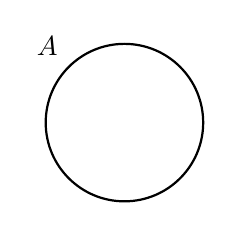
\begin{tikzpicture}[thick]
% Circle with label
\node[draw,
    circle,
    minimum size =2cm,
    label=135:$A$] (circle1) at (0,0){};
\end{tikzpicture} \]

Given two sets $A,B$ there are now four possibilities for all objects in the universe:
\begin{enumerate}
\item outside both $A$ and $B$;
\item inside $A$, but not inside $B$;
\item inside $B$, but not inside $A$;
\item inside both $A$ and $B$.
\end{enumerate}
We correspondingly divide the paper into four regions:
\[ 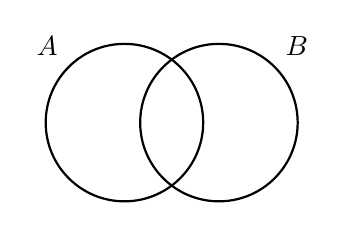
\begin{tikzpicture}[thick]
% Set A
\node [draw,
    circle,
    minimum size =2cm,
    label={135:$A$}] (A) at (0,0){};
% Set B
\node [draw,
    circle,
    minimum size =2cm,
    label={45:$B$}] (B) at (1.2,0){};
\end{tikzpicture} \]

For three sets $A,B,C$ the picture becomes:
\[ 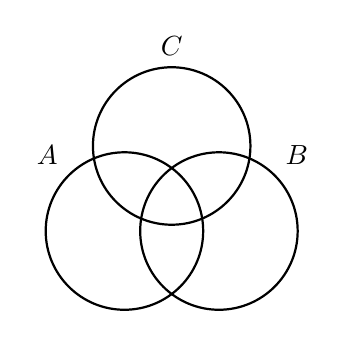
\begin{tikzpicture}[thick]
% Set A
\node[draw,circle,minimum size =2cm,label={135:$A$}] (A) at (0,0) {};

% Set B
\node[draw,circle,minimum size =2cm,label={45:$B$}] (B) at (1.2,0) {};

% Set C
\node[draw,circle,minimum size =2cm,label=$C$] (C) at (0.6,1.08) {};
\end{tikzpicture} \]

If we want to show that one set is a subset of another set, e.g\ $B\subset A$, then we can represent this as follows:
\[ 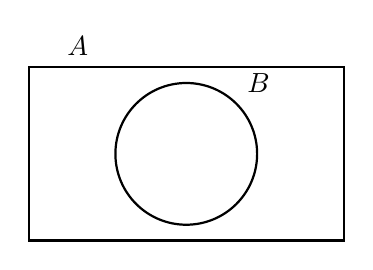
\begin{tikzpicture}[thick]
% Set A
\node [draw,
    rectangle,
    minimum width =4cm,
	minimum height = 2.2cm,
    label={135:$A$}] (A) at (0,0){};
% Set B
\node [draw,
    circle,
    minimum size =1.8cm,
    label={45:$B$}] (B) at (0,0){};
\end{tikzpicture} \]

Expressions talking about sets can be expressed by shading regions of Venn diagrams. For example $A\cup B$:
\[ 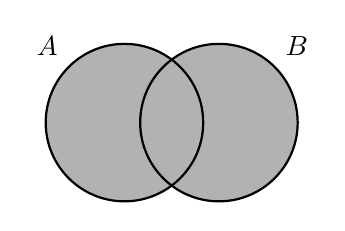
\begin{tikzpicture}[thick,
    set/.style = {circle,
        minimum size = 2cm,
        fill=black!30}]

% Set A
\node[set,label={135:$A$}] (A) at (0,0) {};

% Set B
\node[set,label={45:$B$}] (B) at (1.2,0) {};

% Circles outline
\draw (0,0) circle(1cm);
\draw (1.2,0) circle(1cm);
\end{tikzpicture} \]

\subsection{Operations on sets}
\subsubsection{Intersection}
\begin{definition}
The \udef{intersection} of an object $\mathcal{E}$ is a set $\bigcap \mathcal{E}$ defined by
\[ \bigcap \mathcal{E} \defeq \left\{ x\in \bigcup\mathcal{E} \;|\; \forall X\in \mathcal{E}: x\in X \right\}. \]
\end{definition}
As before, for the union, we define
\[ A\cap B \defeq \bigcap \{A,B\}. \]

The intersection $A\cap B$ can be represented in a Venn diagram as follows:
\[ 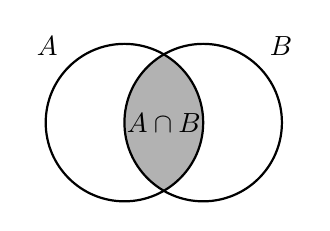
\begin{tikzpicture}[thick,
    set/.style = {circle,
        minimum size = 2cm}]

% Set A
\node[set,label={135:$A$}] (A) at (0,0) {};

% Set B
\node[set,label={45:$B$}] (B) at (1,0) {};

% Intersection
\begin{scope}
    \clip (0,0) circle(1cm);
    \clip (1,0) circle(1cm);
    \fill[black!30](0,0) circle(1cm);
\end{scope}

% Circles outline
\draw (0,0) circle(1cm);
\draw (1,0) circle(1cm);

% Set intersection label
\node at (0.5,0) {$A\cap B$};
\end{tikzpicture} \]

\begin{proposition}
Let $A, B$ be non-empty sets. Then
\begin{enumerate}
\item $A \subseteq B \implies \bigcap B\subseteq \bigcap A$;
\item $\bigcap(A\cup B) = (\bigcap A)\cup (\bigcap B)$.
\end{enumerate}
These statements hold for all sets $A,B$ iff we use an unrelativised intersection (TODO!).
\end{proposition}

\begin{definition}
Let $A,B$ be sets. We call $A$ and $B$ \udef{disjoint} if $A\cap B = \emptyset$. We write $A\perp B$.

A family of sets $\mathcal{E}$ is called \udef{pairwise disjoint} if $\forall A,B\in\mathcal{E}: A\perp B$.
\end{definition}
The notation $A\perp B$ is not standard in general set theory, but is somewhat standard for disjoint elements in lattice theory.

\begin{definition}
Let $A,B$ be sets. We call the union $A\cup B$ a \udef{(inner) disjoint union} if $A$ and $B$ are disjoint. We may write $A\uplus B$ for the union if it is disjoint.

If a family of sets $\mathcal{E}$ is pairwise disjoint, we may denote its union $\biguplus \mathcal{E}$.
\end{definition}

\begin{definition}
Let $\mathcal{A},\mathcal{B}$ be families of sets. We say $\mathcal{A}$ and $\mathcal{B}$ \udef{mesh}, denoted $\mathcal{A} \# \mathcal{B}$ if $A$ and $B$ are not disjoint, $A\cap B \neq \emptyset$, for all $A\in \mathcal{A}$ and $B\in\mathcal{B}$.

We write $A \# \mathcal{B}$ for $\{A\}\# \mathcal{B}$ and $A\# B$ for $\{A\}\#\{B\}$.
\end{definition}

\subsubsection{Difference}
\begin{definition}
Given two objects $A,B$, we define the \udef{difference} as
\[A\setminus B \defeq \setbuilder{x\in A}{x\notin B}. \]
\end{definition}
The difference $A\setminus B$ can be represented in a Venn diagram as follows:
\[ 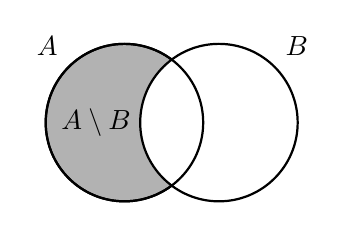
\begin{tikzpicture}[thick,
    set/.style = {circle,
        minimum size = 2cm}]

% Set A
\node[set,draw,fill=black!30,label={135:$A$}] (A) at (0,0) {};

% Set B
\node[set,draw,fill=white,label={45:$B$}] (B) at (1.2,0) {};

% Circles outline
\draw (0,0) circle(1cm);

% Set label
\node at (-0.36,0) {$A\setminus B$};
\end{tikzpicture} \]

\begin{proposition}[De Morgan's laws]
Let $A,B,C$ be sets. Then
\begin{align*}
C\setminus (A\cap B) &= (C\setminus A)\cup(C\setminus B) \\
C\setminus (A\cup B) &= (C\setminus A)\cap(C\setminus B)
\end{align*}
This can be extended to arbitrary families of sets:
\begin{align*}
C\setminus\left(\bigcup \mathcal{E}\right) &= \bigcap\setbuilder{C\setminus A}{A\in\mathcal{E}} \\
C\setminus\left(\bigcap \mathcal{E}\right) &= \bigcup\setbuilder{C\setminus A}{A\in\mathcal{E}}
\end{align*}
where $\mathcal{E}$ is a family of sets.
\end{proposition}
\begin{lemma}
Let $\mathcal{E}$ be a family of sets and $A$ a set. Then
\[ \bigcup \mathcal{E} \setminus A = \bigcup\setbuilder{X\setminus A}{X\in\mathcal{E}} \qquad\text{and}\qquad \bigcap \mathcal{E} \setminus A = \bigcap\setbuilder{X\setminus A}{X\in\mathcal{E}}. \]
\end{lemma}

\begin{lemma} \label{differenceProperties}
Let $A,B,C$ be sets. Then
\begin{enumerate}
\item $(A\setminus B)\setminus C = A\setminus (B\cup C)$;
\item $A\setminus (B\setminus C) = (A\setminus B) \cup (A\cap C)$;
\end{enumerate}
and
\begin{enumerate} \setcounter{enumi}{2}
\item $(A\setminus B)\cap C = (A\cap C)\setminus B = A\cap (C\setminus B)$;
\item $(A\setminus B)\cup C = (A\cup C)\setminus (B\setminus C)$;
\end{enumerate}
and
\begin{enumerate} \setcounter{enumi}{4}
\item $A\setminus A = \emptyset$;
\item $\emptyset\setminus A = \emptyset$;
\item $A\setminus \emptyset = A$.
\end{enumerate}
\end{lemma}

\subsubsection{Symmetric difference}
\begin{definition}
We define the \udef{symmetric difference} of two sets $A,B$ as
\[ A \symdiff B \defeq (A\setminus B)\cup(B\setminus A). \]
This is equivalent to $A\symdiff B = \setbuilder{x\in A\cup B}{(x\in A)\oplus (x\in B)}$.
\end{definition}

The symmetric difference $A\symdiff B$ can be represented in a Venn diagram as follows:
\[ 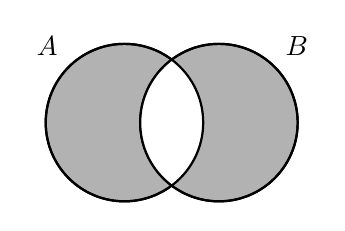
\begin{tikzpicture}[thick,
    set/.style = {circle,
        minimum size = 2cm}]

% Set A
\node[set,draw,fill=black!30,label={135:$A$}] (A) at (0,0) {};

% Set B
\node[set,draw,fill=black!30,label={45:$B$}] (B) at (1.2,0) {};

\begin{scope}
    \clip (0,0) circle(1cm);
    \clip (1.2,0) circle(1cm);
    \fill[white](0,0) circle(1cm);
\end{scope}

% Circles outline
\draw (0,0) circle(1cm);
\draw (1.2,0) circle(1cm);
\end{tikzpicture} \]

\begin{lemma}
Let $A,B,C$ be sets. Then
\begin{align*}
A\symdiff \emptyset &= A \\
A\symdiff B = \emptyset &\iff A = B
\end{align*}
and
\begin{align*}
A \symdiff B &= B \symdiff A \\
(A \symdiff B) \symdiff C &= A \symdiff (B \symdiff C) \\
A \symdiff C &= (A \symdiff B)\symdiff(B \symdiff C).
\end{align*}
\end{lemma}

\subsection{Identities and equivalences}
\subsubsection{Identities involving families of sets}
\begin{lemma}
Let $\mathcal{F}, \mathcal{G}$ be families of sets such that $\mathcal{F}\subseteq \mathcal{G}$. Then
\begin{enumerate}
\item $\bigcup \mathcal{F} \subseteq \bigcup \mathcal{G}$;
\item $\bigcap \mathcal{F} \supseteq \bigcup \mathcal{G}$.
\end{enumerate}
\end{lemma}

\subsubsection{Set operations and statements characterised}
\begin{lemma}
Let $A,B$ be sets. Then
\begin{enumerate}
\item $\begin{aligned}[t]
A\cap B &= A\setminus (A\setminus B) \\
&= B\setminus (A\symdiff B) \\
&= A\symdiff (A\setminus B);
\end{aligned}$
\item $\begin{aligned}[t]
A\cup B &= (A\symdiff B)\cup A \\
&= (A\symdiff B)\symdiff(A\cap B) \\
&= (A\setminus B)\cup B;
\end{aligned}$
\item $\begin{aligned}[t]
A\symdiff B &= (A\cup B)\setminus (A\cap B) \\
&= (A\symdiff C)\symdiff(C\symdiff B)
\end{aligned}$

for any set $C$;
\item $\begin{aligned}[t]
A\setminus B &= A\setminus (A\cap B) \\
&= A\cap(A\symdiff B) \\
&= (A\cup B)\symdiff B \\
&= A\symdiff (A\cap B);
\end{aligned}$
\end{enumerate}
\end{lemma}

\begin{lemma}
Let $A$ be a set. Then the following are equivalent:
\begin{enumerate}
\item $A$ is empty;
\item $A\cup B\subseteq B$ for every set $B$;
\item $A\subseteq B$ for every set $B$;
\item $A\subseteq (B\setminus A)$ for some set $B$;
\item $A\subseteq (B\setminus A)$ for every set $B$;
\item $\emptyset \setminus A= A$.
\end{enumerate}
\end{lemma}

\begin{lemma} \label{inclusionCriteria}
Let $A,B$ be sets. Then following are equivalent:
\begin{enumerate}
\item $A\subseteq B$;
\item $A\cap B = A$;
\item $A\cup B = B$;
\item $A\symdiff B = B\setminus A$;
\item $A\symdiff B \subseteq B\setminus A$
\item $A\setminus B = \emptyset$.
\end{enumerate}
For any universe set $\Omega$ such that $A,B\subset \Omega$ the above is also equivalent to
\begin{enumerate}\setcounter{enumi}{4}
\item $\Omega\setminus B \subseteq \Omega\setminus A$;
\item $(\Omega\cap A)\setminus B = \emptyset$;
\item $(\Omega\setminus A)\cup B = \Omega$.
\end{enumerate}
\end{lemma}
\begin{corollary}
Let $A,B$ be sets. Then following are equivalent:
\begin{enumerate}
\item $A=B$;
\item $A\symdiff B = \emptyset$;
\item $A\setminus B = B\setminus A$.
\end{enumerate}
\end{corollary}
\begin{corollary} \label{setPerpInequality}
Let $A,B\subseteq \Omega$ be sets. Then following are equivalent:
\begin{enumerate}
\item $A\perp B$;
\item $A \subseteq \Omega\setminus B$;
\item $B \subseteq \Omega\setminus A$.
\end{enumerate}
\end{corollary}

\subsubsection{Distributivity}
TODO: tables complete / correct?? TODO: only works for relativised intersection.
\begin{lemma}
We say $*$ left distributes over $\bullet$ if
\[ A*(B\bullet C) = (A*B)\bullet (A*C) \qquad\text{for all sets $A,B,C$.} \]
This gives the table
\[ \begin{array}{c | c c c c c}
\text{\diagbox{$*$}{$\bullet$}} & \cup & \cap & \symdiff & \setminus & \times \\ \hline
\cup & \checkmark & \checkmark &  & & \\
\cap & \checkmark & \checkmark & \checkmark & \checkmark & \\
\symdiff &  &  &  & & \\
\setminus &  &  &  & & \\
\times & \checkmark & \checkmark &  & \checkmark &
\end{array} \]
\end{lemma}

\begin{lemma}
We say $*$ right distributes over $\bullet$ if
\[ (A\bullet B)*C = (A*C)\bullet (B*C) \qquad\text{for all sets $A,B,C$.} \]
This gives the table
\[ \begin{array}{c | c c c c c}
\text{\diagbox{$*$}{$\bullet$}} & \cup & \cap & \symdiff & \setminus & \times \\ \hline
\cup & \checkmark & \checkmark &  & & \\
\cap & \checkmark & \checkmark & \checkmark & \checkmark & \\
\symdiff &  &  &  & & \\
\setminus & \checkmark & \checkmark & \checkmark & \checkmark & \\
\times & \checkmark & \checkmark &  & \checkmark &
\end{array} \]
\end{lemma}

TODO: intersection distributes over disjoint union.

\begin{lemma} \label{unionIntersectionLabelSet}
Let $\mathcal{I}$ be a family of index sets and let $A_i$ be a set for all $i\in \bigcup \mathcal{I}$. Then
\begin{enumerate}
\item $\bigcup_{i\in \bigcup \mathcal{I}} A_i = \bigcup_{I\in \mathcal{I}}\bigcup_{i\in I} A_i$;
\item $\bigcap_{i\in \bigcap \mathcal{I}} A_i = \bigcap_{I\in \mathcal{I}}\bigcap_{i\in I} A_i$;
\item $\bigcup_{i\in \bigcap \mathcal{I}} A_i \subseteq \bigcap_{I\in \mathcal{I}}\bigcup_{i\in I} A_i$;
\item $\bigcap_{i\in \bigcup \mathcal{I}} A_i \supseteq \bigcup_{I\in \mathcal{I}}\bigcap_{i\in I} A_i$.
\end{enumerate}
\end{lemma}
\begin{proof}
(1) We calculate
\begin{align*}
x\in \bigcup_{i\in \bigcup \mathcal{I}} A_i &\iff \exists i\in \bigcup \mathcal{I}: x\in A_i \\
&\iff \exists i: (i\in \bigcup \mathcal{I}) \land (x\in A_i) \\
&\iff \exists i: (\exists I \in \mathcal{I}: i\in I) \land (x\in A_i) \\
&\iff \exists i: \exists I: (I \in \mathcal{I}) \land (i\in I) \land (x\in A_i) \\
&\iff \exists I\in \mathcal{I}: \exists i \in I: x\in A_i \\
&\iff x\in \bigcup_{I\in \mathcal{I}}\bigcup_{i\in I} A_i
\end{align*}

(2) Replace $\exists$ by $\forall$ and $\land$ by $\Rightarrow$ in the proof of (1).

(3) We calculate
\begin{align*}
x\in \bigcup_{i\in \bigcap \mathcal{I}} A_i &\iff \exists i\in \bigcap \mathcal{I}: x\in A_i \\
&\iff \exists i: (i\in \bigcap \mathcal{I}) \land (x\in A_i) \\
&\iff \exists i: (\forall I \in \mathcal{I}: i\in I) \land (x\in A_i) \\
&\iff \exists i: (\forall I: (I \in \mathcal{I}) \Rightarrow (i\in I)) \land (x\in A_i) \\
&\implies \exists i: \forall I: (I \in \mathcal{I}) \Rightarrow ((i\in I) \land (x\in A_i)) \\
&\implies \forall I: \exists i: (I \in \mathcal{I}) \Rightarrow ((i\in I) \land (x\in A_i)) \\
&\iff \forall I: (I \in \mathcal{I}) \Rightarrow (\exists i:(i\in I) \land (x\in A_i)) \\
&\iff \forall I\in \mathcal{I}: \exists i \in I: x\in A_i \\
&\iff x\in \bigcap_{I\in \mathcal{I}}\bigcup_{i\in I} A_i
\end{align*}

(4) TODO
\end{proof}

For more identities, see \url{https://en.wikipedia.org/wiki/List_of_set_identities_and_relations}.


\chapter{Relations and functions}
\section{Pairs}
\begin{definition}
A definition of $(a,b)$ for all $a,b$ is called an \udef{(ordered) pair operation} if it satisfies
\begin{itemize}
\item $(a,b) = (x,y) \iff (a=x)\land (b=y)$;
\item for all sets $A,B$, $\setbuilder{(a,b)}{a\in A\land b\in B}$ is a set.
\end{itemize}
We call $\setbuilder{(a,b)}{a\in A\land b\in B}$ the \udef{Cartesian product} of classes $A$ and $B$ and denote it $A\times B$.
\end{definition}
Note that for the second condition it is enough to check that $A\times B$ is a subset of some set $S$. Then, by separation, $A\times B$ is the set
\[ A\times B = \setbuilder{x\in S}{\exists a\in A:\exists b\in B: x = (a,b)}. \]

\begin{lemma}
Let $A$ be a class. Then
\[ A\times \emptyset = \emptyset = \emptyset\times A. \]
\end{lemma}

\begin{lemma} \label{productUnionIntersection}
Let $A,B,C,D$ be classes. Then
\begin{enumerate}
\item $(A\cup B)\times C = A\times C \cup B\times C$;
\item $(A\uplus B)\times C = A\times C \uplus B\times C$;
\item $(A\cap B)\times C = A\times C\cap B\times C$;
\item $(A\times B)\cap (C\times D) = (A \cap C)\times (B\cap D)$.
\end{enumerate}
\end{lemma}

\begin{definition}
Let $p = (a,b)$ be a pair, we use $\pi_1(p)$ to denote the first element of $p$ and $\pi_2(p)$ to denote the second element:
\[ (a,b) = p = (\pi_1(p),\pi_2(p)). \]
We can convert a pair to a set:
\[ \operatorname{set}((a,b)) = \{a,b\}. \]
\end{definition}


\subsection{Axiomatising pairs}
Consider the ternary proposition $A = (B,C)$ as primitive. 
\begin{definition}
Consider a universe $\mathcal{W}$. Let $p$ be an object in $\mathcal{W}$. We call $p$ a \udef{pair} if $\exists x,y: p = (x,y)$.

We define the predicate
\begin{itemize}
\item $\Pair(p) \defequiv \exists x,y: \; p = (x, y)$.
\end{itemize}
\end{definition}

\begin{enumerate}[(A)] \setcounter{enumi}{0}
\item \textbf{Axiom of pair identity}: Let $p_1, p_2,x_1,x_2,y_1,y_2$ be objects such that
\[ p_1 = (x_1, y_1) \qquad \text{and}\qquad p_2 = (x_2, y_2). \]
Then
\[ p_1 = p_2 \quad\iff\quad \big[x_1 = x_2\big] \;\land\; \big[y_1 = y_2\big]. \]
\item \textbf{Axiom of pair existence}: Let $x,y$ be objects. Then $\exists p: \; p = (x,y)$ with $p\neq x $ and $p \neq y$.
\end{enumerate}

\begin{lemma}
Let $x,y$ be objects. Then $\exists! p: \; p = (x,y)$ with $p\neq x $ and $p \neq y$.
\end{lemma}
\begin{proof}
Existence is given by the axiom of pair existence. We just need to show uniqueness. Assume there exist $p_1, p_2$ such that $p_1 = (x,y)$ and $p_2 = (x,y)$. Then $p_1 = p_2$ by the axiom of pair identity.
\end{proof}

Usually an axiomatic system of pairs is integrated with a set theory.
\begin{definition}
Let $\mathcal{W}$ be a set theoretic universe satisfying the pair axioms. Let $A,B$ be classes. The \udef{Cartesian product} of $A$ and $B$ is defined as
\[ A\times B \defeq \setbuilder{p}{\exists a\in A: \exists b\in B: p = (a,b)}. \]
\end{definition}

In this case we impose the following additional axioms:
\begin{enumerate}[(A)] \setcounter{enumi}{2}
\item \textbf{Axiom of element pairs}: Let $a,b$ be elements and $p=(a,b)$. Then $p$ is an element.
\item \textbf{Cartesian product axiom}: Let $A,B$ be sets. Then $A \times B$ is a set.
\end{enumerate}

\begin{lemma}
Let $A, B$ be classes $a\in A, b\in B$ and $p = (a,b)$. Then $p\in A\times B$.
\end{lemma}
\begin{proof}
In this case $a,b$ are elements. So $p$ is an element by the axiom of element pairs and thus $p\in A\times B$ by class comprehension.
\end{proof}


\subsection{Defining pairs}
TODO: pair axioms conservative extension of ZFC.

\subsubsection{The Kuratowski pair}
\begin{definition}
The \udef{Kuratowski pair} is defined as
\[ (a,b) \defeq \{\{a\}, \{a,b\}\} \]
\end{definition}
Note that when $a=b$ we have
\[ (a,a) = \{\{a\},\{a,a\}\} = \{\{a\},\{a\}\} = \{\{a\}\}. \]
\begin{lemma}
Given a Kuratowski pair $p = (a,b)$, we can extract the first element $\pi_1(p)$ and the second element $\pi_2(p)$ as follows:
\begin{align*}
\pi_1(p) &= \bigcup\bigcap p; \\
\pi_2(p) &= \bigcup\left\{ x\in\bigcup p\;|\; \left[\bigcup p \neq \bigcap p\right] \implies \left[ x\notin \bigcap p \right] \right\}.
\end{align*}
The Kuratowski pair can be converted to a set by
\[ \operatorname{set}(p) = \bigcup p. \]
\end{lemma}
The construction ``$\left[\bigcup p \neq \bigcap p\right] \implies$'' in the formula for $\pi_2(p)$ is there so that it still works in case the first and second elements are the same.
\begin{proposition}
The Kuratowski pair is adequate, in that is satisfies
\[ (a,b) = (x,y) \iff (a=x)\land (b=y) \]
and the Cartesian product is a set.
\end{proposition}
\begin{proof}
If $(a=x)\land (b=y)$, then
\[ \{\{a\},\{a,b\}\} = \{\{x\},\{x,y\}\} \]
and thus $(a,b) = (x,y)$.

Now assume $(a,b) = (x,y)$. We consider two cases: $a=b$ and $a\neq b$.
\begin{itemize}[leftmargin=2cm]
\item[$\boxed{a=b}$] Then $(a,b) = \{\{a\},\{a,a\}\} = \{\{a\}\} = (x,y)$ and thus $\{x\} = \{x,y\} = \{a\}$ by extensionality. This implies $a=x=y$ and thus $(a=x)\land (b=y)$.
\item[$\boxed{a\neq b}$] Now $(a,b) = (x,y)$ implies
\[ \{\{a\},\{a,b\}\} = \{\{x\},\{x,y\}\}. \]
By extensionality, either $\{x\} = \{a\}$ or $\{x\} = \{a,b\}$. In the second option $a=x=b$ and thus $a=b$ which is a contradiction. So $x=a$.

Again by extensionality, either $\{x,y\} = \{a\}$ or $\{x,y\} = \{a,b\}$. In the first case $(x,y)$ would be a singleton and then by equality so would $(a,b)$, yielding a contradiction. Thus $\{x,y\} = \{a,b\}$. We know $a=x$ and $b\neq a$, so by extensionality $b=y$.
\end{itemize}
To prove the Cartesian product $A\times B$ is a set, notice that
\begin{align*}
a\in A, b\in B &\implies \{a\},\{a,b\}\subseteq A\cup B \implies \{a\},\{a,b\}\in \powerset(A\cup B)\\
&\implies \{\{a\},\{a,b\}\}\subseteq \powerset(A\cup B) \implies \{\{a\},\{a,b\}\}\in \powerset(\powerset(A\cup B)) \\
&\implies (a,b) \in \powerset(\powerset(A\cup B)).
\end{align*}
and $\powerset(\powerset(A\cup B))$ is a set. So
\[ A\times B = \{ x\in \powerset(\powerset(A\cup B))\;|\; \exists a\in A:\exists b\in B: x = (a,b) \} \]
is a set.
\end{proof}
\subsubsection{The short variant}
We can also define a pair as
\[ (a,b) \defeq \{a,\{a,b\}\} \]
The advantage of this short definition is fewer braces. Some disadvantages include:
\begin{enumerate}
\item If $a$ and $b$ have the same type, $a$ and $\{a,b\}$ do not have the same type.
\item In order to prove adequacy, we need a new axiom, the axiom of regularity.
\end{enumerate}
\subsubsection{Using $0,1$}
Suppose we have decided on two special, distinct objects $0,1$. Then we can define
\[ (a,b) \defeq \{\{0,a\},\{1,b\}\}. \]
\begin{proposition}
This definition satisfies the requirements for a pair.
\end{proposition}
\begin{proof}
Assuming $(a=x)\land (b=y)$, it is clear that $(a,b)=(x,y)$ as sets by extensionality.

Now assume $(a,b)=(x,y)$. In this implementation a pair always has two elements as a set. The reasoning by extensionality is simple and only slightly more difficult if $a,b,x,y$ are equal to $0$ or $1$.

The Cartesian product is a subset of $\powerset(\powerset(A\cup B\cup \{0,1\}))$ and thus a set.
\end{proof}
\subsubsection{Wiener pair}
The Wiener definition of a pair is
\[ (a,b) \defeq \{\{\emptyset,\{a\}\},\{\{b\}\}\}. \]
\begin{proposition}
This definition satisfies the requirements for a pair.
\end{proposition}

\subsection{Structured classes and sets}
\begin{definition}
A \udef{structured class} is a pair $U = (A,S)$ where $A$ is a class and $S$ is an arbitrary object.
\begin{itemize}
\item $A$ is the \udef{field} or \udef{space} of $U$, written $\operatorname{Field}(U)$;
\item $S$ is the \udef{frame} of $U$.
\end{itemize}
If we write $x\in U$, we mean $x\in \operatorname{Field}(U)$.

In particular if $A$ is a set, then we call $U$ a \udef{structured set}.
\end{definition}

Often the frame $S$ is a $n$-tuple. In this case we may write the structured class as an $n+1$-tuple by concatenating the field and the frame. e.g\ $(A,(S_1,S_2,S_3))$ becomes $(A,S_1,S_2,S_3)$.

\section{Relations}
\begin{definition}
Let $A,B$ be classes and $G$ any subclass of the Cartesian product $A\times B$. A \udef{(binary) relation} $R$ on $(A, B)$ is a tuple $(G,(A,B))$. The \udef{graph} of the binary relation $R$ is the class $\graph(R) \defeq G$.

We write
\[ xRy \defequiv (x,y)\in \graph(R) \]
and say $x$ is \udef{left related} to $y$ or $y$ is \udef{right related} to $x$.

We call
\begin{itemize}
\item $\dom(R) \defeq A$ the \udef{domain} of the relation;
\item $\codom(R) \defeq B$ the \udef{codomain} of the relation.
\end{itemize}
A relation $R$ is \udef{homogeneous} or an \udef{endorelation} if $\dom(R) = \codom(R)$.
If we say $R$ is a (homogenous) relation on $A$, we mean $\dom(R) = A = \codom(R)$. 

A relation is \udef{heterogeneous} is the domain and codomain are different.
\end{definition}

Often we will write $R \subseteq S$ as a shorthand for $\graph(R)\subseteq \graph(S)$.

\begin{lemma}
Let $R,S$ be relations on $(A,B)$. Then
\begin{enumerate}
\item $R\cup S \defeq \sSet{\graph(R)\cup \graph(S), (A,B)}$ is a relation on $(A,B)$;
\item $R\cap S \defeq \sSet{\graph(R)\cap \graph(S), (A,B)}$ is a relation on $(A,B)$.
\end{enumerate}
\end{lemma}

\begin{definition}
Let $A,B$ be classes. We have the following relations:
\begin{itemize}
\item the \udef{empty relation} $E_{A,B}$ on $(A, B)$ has graph $\emptyset$;
\item the \udef{universal relation} $U_{A,B}$ on $(A, B)$ has graph $A\times B$;
\item the \udef{identity relation} $\id_A$ on $A$ has graph $\setbuilder{(x,y)\in A\times A}{x=y}$.
\end{itemize}
We may also write $U_A$ instead of $U_{A,A}$ and $E_A$ instead of $E_{A,A}$.
\end{definition}
The identity relation on $A$ is also known as the \udef{diagonal relation} on $A$.

\begin{lemma}
Let $A,B,C,D$ be classes. Then
\begin{enumerate}
\item $\id_{A\cup B} = \id_A\cup \id_B$ and $\id_{A\cap B} = \id_A\cap \id_B$;
\item $E_{A\cup C, B\cup D} = E_{A,B}\cup E_{C,D}$ and $E_{A\cap C, B\cap D} = E_{A,B}\cap E_{C,D}$;
\item $U_{A\cap C, B\cap D} = U_{A,B}\cap U_{C,D}$.
\end{enumerate}
\end{lemma}
Note that the equalities mean the graphs are equal. The relations are not the same as they have different domains and codomains.
\begin{proof}
(1) Assume $(x,x)\in \id_{A\cup B}$. We have the equivalences
\[ (x\in A)\lor (x\in B) \iff \Big((x,x)\in \id_A\Big) \lor \Big((x,x)\in\id_B\Big) \iff (x,x)\in \id_A\cup \id_B. \]
For the second part replace $\lor$ with $\land$.

(2) Trivial because all sets are $\emptyset$.

(3) Take $(x,y)\in U_{A\cap C, B\cap D}$. We have the equivalences
\begin{align*}
(x\in A\cap C) \land (y\in B\cap D) &\iff (x\in A)\land (y\in B)\land(x\in C)\land(y\in D) \\
&\iff \big((x,y)\in U_{A, B})\big)\land\big((x,y)\in U_{A, B}\big) \\
&\iff (x,y)\in U_{A,B}\cap U_{C,D}.
\end{align*}
\end{proof}


\begin{definition}
Let $R$ be a binary relation. We say
\begin{itemize}
\item $x$ is \udef{related to} or \udef{comparable with} $y$ if $xRy$ or $yRx$; we denote this $x\nparallel_R y$ or just $x\nparallel y$;
\item $x$ is \udef{unrelated to}, \udef{incomparable with} or \udef{parallel with} $y$ if neither $xRy$ nor $yRx$; we denote this $x\parallel_R y$ or just $x\parallel y$.
\end{itemize}
\end{definition}

\subsection{Relations and subclasses}
\subsubsection{Images and preimages}
\begin{definition}
Let $R$ be a relation on $(A, B)$.
\begin{itemize}
\item The \udef{image} of a subclass $X\subset A$ under $R$ is the class
\[ X_R \defeq \setbuilder{b\in B}{\exists x\in X: xRb}. \]
\item The \udef{preimage} of a subclass $Y\subset B$ under $R$ is the class
\[ _RY \defeq \setbuilder{a\in A}{\exists y\in Y: aRy}. \]
\end{itemize}
In particular for $X=A$ and $Y=B$:
\begin{enumerate}
\item The class $A_R$ is the \udef{active codomain}, \udef{codomain of definition}, \udef{image} or \udef{range} of the relation, also denoted $\im(R)$.
\item The class $_RB$ is the \udef{active domain}, \udef{domain of definition}, \udef{preimage} or \udef{prerange} of the relation, also denoted $\preim(R)$.
\end{enumerate}
In particular for $X = \{x\}$ and $Y = \{y\}$ we define:
\begin{itemize}
\item $xR \defeq \{x\}_R$;
\item $Ry \defeq {_R\{x\}}$.
\end{itemize}
We call such images and preimages \udef{principle} images and preimages.
\end{definition}

A relation is completely characterised by its principal images.
\begin{lemma} \label{relationFromPrincipalImages}
Let $R$ be a relation on $(A, B)$, $x\in A$ and $y\in B$. Then
\[ x\in Ry \iff xRy \iff xR \ni y. \]
\end{lemma}
Principal images atoms in lattice of images??

\begin{lemma}
Let $R$ be a relation on $(A, B)$, $X\subseteq A$ and $Y\subseteq B$. Then
\begin{enumerate}
\item $X_R = {_{R^\transp}X}$;
\item $_RX = X_{R^\transp}$.
\end{enumerate}
In particular $xR = R^\transp x$ and $Ry = yR^\transp$ for all $x\in A$ and $y\in B$.
\end{lemma}

TODO: atomicity / atomistic ??
\begin{lemma}
Let $R$ be a relation on $(A, B)$, $X\subseteq A$ and $Y\subseteq B$. Then
\begin{enumerate}
\item $X_R = \displaystyle\bigcup_{x\in X}xR = \bigcup \setbuilder{xR}{x\in X}$;
\item $_RY = \displaystyle\bigcup_{y\in Y}Ry = \bigcup \setbuilder{Ry}{y\in Y}$.
\end{enumerate}
\end{lemma}


\begin{corollary} \label{monotonicityImage}
Let $R$ be a relation on $(A, B)$ and $X,Y\subset A$. Then
\begin{enumerate}
\item if $X\subseteq Y$, then $X_R \subseteq Y_R$;
\item if $X\subseteq Y$, then ${_RX} \subseteq {_RY}$.
\end{enumerate}
\end{corollary}
\begin{proof}
(1) We can write $Y = X \cup (Y\setminus X)$. Then
\[ Y_R = \bigcup \setbuilder{xR}{x\in Y} = \bigcup \setbuilder{xR}{x\in X}\cup\setbuilder{xR}{x\in (Y\setminus X)} = X_R \cup (Y\setminus X)_R \supseteq X_R. \]

(2) Similar.
\end{proof}
\begin{corollary} \label{imageRelation} \label{preimageRelation}
Let $R$ be a relation on $(A, B)$, $X,Y\subset A$ and $Z,W\subset B$. Then
\begin{enumerate}
\item $(X\cup Y)_R = X_R\cup Y_R$;
\item $(X\cap Y)_R \subseteq X_R\cap Y_R$;
\item $(X\setminus Y)_R \supseteq X_R\setminus Y_R$;
\item $(X\symdiff Y)_R \supseteq X_R\symdiff Y_R$.
\end{enumerate}
and
\begin{enumerate}
\item $_R(Z\cup W) = {_RZ}\cup {_RW}$;
\item $_R(Z\cap W) \subseteq {_RZ}\cap {_RW}$;
\item $_R(Z\setminus W) \supseteq {_RZ}\setminus {_RW}$;
\item $_R(Z\symdiff W) \supseteq {_RZ}\symdiff {_RW}$.
\end{enumerate}
\end{corollary}
\begin{proof}\mbox{}

(1) $\begin{aligned}[t]
(X\cup Y)_R &= \bigcup \setbuilder{xR}{x\in (X\cup Y)} = \bigcup \setbuilder{xR}{x\in X}\cup \setbuilder{xR}{x\in Y} \\
&= \left(\bigcup \setbuilder{xR}{x\in X}\right)\cup \left(\bigcup \setbuilder{xR}{x\in Y}\right) = X_R \cup Y_R.
\end{aligned}$

(2) We have both $X\cap Y \subseteq X$ and $X\cap Y \subseteq Y$, so $(X\cap Y)_R \subseteq X_R$ and $(X\cap Y)_R \subseteq Y_R$ by \ref{monotonicityImage}. Thus $(X\cap Y)_R \subseteq X_R\cap Y_R$.

TODO: use lattice properties

(3), (4) TODO
\end{proof}


\subsubsection{Left and right bounds}
\begin{definition}
Let $R$ be a relation on $(A, B)$, $X\subseteq A$ and $Y\subseteq B$.
\begin{itemize}
\item A \udef{right bound} (or \udef{upper bound}) of $X$ under $R$ is an element $b\in B$ such that $b$ is right related to all $x\in X$. We denote the class of right bounds by
\[ X^R \defeq \setbuilder{b\in B}{\forall x\in X: xRb}. \]
\item A \udef{left bound} (or \udef{lower bound}) of $Y$ under $R$ is an element $a\in A$ such that $a$ is left related to all $y\in Y$. We denote the class of left bounds by
\[ ^RY \defeq \setbuilder{a\in A}{\forall y\in Y: aRy}. \]
\end{itemize}
The classes $X^R$ and $^RY$ are also called \udef{polars}.\footnote{According to Birkhoff (TODO ref), the term ``polar'' was chosen due to the link with the polars of conic sections.}

In particular for $X=A$ and $Y=B$:
\begin{enumerate}
\item The class $A^R$ is referred to as the \udef{top} of $\sSet{R,(A,B)}$.
\item The class $^RB$ is the \udef{bottom} of $\sSet{R,(A,B)}$.
\end{enumerate}
\end{definition}
Note that the definitions of the polars is similar to the definition of the image/preimage. The only difference is that ``$\exists$'' is replaced by ``$\forall$''.

Consequently, we can state results similar to the ones above.

\begin{lemma}
Let $R$ be a relation on $(A, B)$, $X\subset A$ and $Y\subset B$. Then
\begin{enumerate}
\item $X^R = {^{R^\transp}X}$;
\item $^RX = X^{R^\transp}$.
\end{enumerate}
\end{lemma}

\begin{lemma} \label{boundsFromPrincipalImages}
Let $R$ be a relation on $(A, B)$, $X\subset A$ and $Y\subset B$. Then
\begin{enumerate}
\item $X^R = \displaystyle\bigcap_{x\in X}xR = \bigcap \setbuilder{xR}{x\in X}$;
\item $^RY = \displaystyle\bigcap_{y\in Y}Ry = \bigcap \setbuilder{Ry}{y\in Y}$.
\end{enumerate}
In particular for $x\in A$ and $y\in B$:
\begin{enumerate}
\item $\{x\}^R = xR = \{x\}_R$;
\item $^R\{y\} = Ry = {_R\{y\}}$.
\end{enumerate}
\end{lemma}
TODO this only works for empty sets if we relativise the intersection!

\begin{lemma} \label{polarsCartesianProduct}
Let $R$ be a relation on $(A,B)$ and $X\subseteq A, Y\subseteq B$. Then
\[ Y\subseteq X^R \iff X\times Y \subseteq R. \]
\end{lemma}

\begin{corollary} \label{monotonicityPolars}
Let $R$ be a relation on $(A, B)$ and $X,Y\subset A$. Then
\begin{enumerate}
\item if $X\subseteq Y$, then $X^R \supseteq Y^R$;
\item if $X\subseteq Y$, then ${^RX} \supseteq {^RY}$.
\end{enumerate}
\end{corollary}
\begin{proof}
(1) We can write $Y = X \cup (Y\setminus X)$. Then
\[ Y^R = \bigcap \setbuilder{xR}{x\in Y} = \bigcap \setbuilder{xR}{x\in X}\cap\setbuilder{xR}{x\in (Y\setminus X)} = X^R \cap (Y\setminus X)^R \subseteq X^R. \]

(2) Similar.
\end{proof}
\begin{corollary} \label{polarasRelation}
Let $R$ be a relation on $(A, B)$, $X,Y\subset A$ and $Z,W\subset B$. Then
\begin{enumerate}
\item $(X\cup Y)^R \subseteq X^R\cap Y^R$;
\item $(X\cap Y)^R \supseteq X^R\cup Y^R$;
\item $(X\setminus Y)^R ? X^R\setminus Y^R$;
\item $(X\symdiff Y)^R ? X^R\symdiff Y^R$.
\end{enumerate}
and
\begin{enumerate}
\item $^R(Z\cup W) \subseteq {^RZ}\cup {^RW}$;
\item $^R(Z\cap W) \supseteq {^RZ}\cap {^RW}$;
\item $^R(Z\setminus W) ? {^RZ}\setminus {^RW}$;
\item $^R(Z\symdiff W) ? {^RZ}\symdiff {^RW}$.
\end{enumerate}
\end{corollary}
\begin{proof}\mbox{}
(1) We have both $X\cup Y \supseteq X$ and $X\cup Y \supseteq Y$, so $(X\cup Y)^R \subseteq X^R$ and $(X\cup Y)^R \subseteq Y^R$ by \ref{monotonicityImage}. Thus $(X\cup Y)^R \subseteq X^R\cap Y^R$.

(2) TODO ref order reversing function on lattice.

(3), (4) TODO
\end{proof}

\subsubsection{Extending the relation to powersets}
\begin{definition}
Let $R$ be a relation on $(A,B)$. Let $X\subseteq A$ and $Y\subseteq B$ be classes. Then we write $X\aset{R}Y$ if
\[ \forall x\in X: \forall y\in Y: \; xRy. \]
\end{definition}

\begin{lemma}
Let $R$ be a relation on $(A,B)$. Let $X\subseteq A$ and $Y\subseteq B$ be classes. Then
\[ X \aset{R} Y \quad\iff\quad X \subseteq {^RY} \quad\iff\quad Y \subseteq X^R. \]
\end{lemma}

\subsubsection{Greatest and least elements}
\begin{definition}
Let $\sSet{A, R}$ be a relational structure and $X\subseteq A$ a subset.
\begin{itemize}
\item A \udef{greatest element}, \udef{largest element} or \udef{maximum} of $X$ is an upper bound of $X$ that is an element of $X$. We denote the class of maxima by $\max(X) \defeq X^R\cap X$.
\item A \udef{least element}, \udef{smallest element} or \udef{minimum} of $X$ is a lower bound of $X$ that is an element of $X$. We denote the class of minima by $\min(X) \defeq {^RX}\cap X$.
\end{itemize}
We also call
\begin{itemize}
\item an element of $\sup(S) \defeq \min(X^R) = X^R \cap (X^R)^{R^\transp}$ a \udef{least upper bound}, \udef{supremum}, or \udef{join};
\item an element of $\inf(S) \defeq \max({^RX}) = X^{R^\transp} \cap (X^{R^\transp})^R$ a \udef{greatest lower bound}, \udef{infimum}, or \udef{meet}.
\end{itemize}
\end{definition}

\begin{lemma} \label{minMaxSingletons}
If $\sSet{A, R}$ is an anti-symmetric relational structure and $X\subseteq A$, then $\max(X), \min(X), \sup(X)$ and $\inf(X)$ are either singletons or empty.
\end{lemma}
\begin{proof}
We prove for $\max(X)$. The other cases follow dually or a fortiori. Let $x,y\in \max(X)$. Then $xRy$ and $yRx$, so $x=y$ by anti-symmetry.
\end{proof}
In this case we use $\max/\min/\sup/\inf$ to denote the contents of the singleton rather than the singleton itself. If the set is empty, we say the $\max/\min/\sup/\inf$ does not exist.

\begin{lemma} \label{greatestLeastElementsSubsetPoset}
Let $\sSet{P, \precsim}$ be a poset and $R\subseteq S\subseteq P$.
\begin{enumerate}
\item If $\max(R)$ and $\max(S)$ exists, then $\max(R) \precsim \max(S)$.
\item If $\min(R)$ and $\min(S)$ exists, then $\min(R) \succsim \min(S)$.
\end{enumerate}
\end{lemma}
\begin{proof}
By definition $\max(S) \succsim x$ for all $x \in S$. Now $\max(R)\in R\subseteq S$, so in particular $\max(R) \precsim \max(S)$.
\end{proof}

TODO: set to class?
\begin{lemma} \label{maxSupMinInf}
If $\sSet{P, \Yleft}$ is an ordered set and $S\subseteq P$, then
\begin{enumerate}
\item $\max(S)\subset \sup(S)$;
\item $\min(S)\subset \inf(S)$.
\end{enumerate}
\end{lemma}
\begin{proof}
For (1) we calculate $\max(S) = S \cap S^u \subseteq (S^u)^l \cap S^u = \sup(S)$; (2) is dual.

TODO: post Galois??
\end{proof}

\subsubsection{Maxima and minima}
\begin{definition}
$X^{R\cup \overline{R}^\transp}\cap X$ (if anti-asymmetric = $X^{\overline{R}^\transp}\cap X$).

A \udef{maximal element} of $S$ is an element $x\in S$ such that no element $y$ is strictly greater than $x$
\end{definition}

\subsection{Converse relation}
\begin{definition}
Let $R$ be a relation on $(A, B)$. The \udef{converse} $R^\transp$ of $R$ is the relation on $B\times A$ with graph
\[ \graph(R^{\transp}) = \setbuilder{(y,x)}{(x,y)\in \graph(R)} \subset B\times A. \]
It is also known as the \udef{inverse}, \udef{transpose}, \udef{reciprocal}, \udef{opposite} or \udef{dual} of $R$.
\end{definition}

\begin{lemma}
Let $R,S$ be relations on $(A, B)$, $X\subseteq A$ and $Y\subseteq B$. Then
\begin{enumerate}
\item $(R^\transp)^\transp = R$;
\item $(R \cup S)^\transp = R^\transp \cup S^\transp$;
\item $(R \cap S)^\transp = R^\transp \cap S^\transp$;
\item $\dom(R^\transp) = \codom(R)$ and $\codom(R^\transp) = \dom(R)$;
\item $_{R^\transp}X = X_R$ and $Y_{R^\transp} = {_RY}$;
\item $\im(R^\transp) = \preim(R)$;
\item if $R\subseteq S$, then $R^\transp \subseteq S^\transp$.
\end{enumerate}
\end{lemma}

\begin{lemma}
Let $A,B$ be classes. Then
\begin{enumerate}
\item $U_{A,B}^\transp = U_{B,A}$;
\item $E_{A,B}^\transp = E_{B,A}$;
\item $\id_A^\transp = \id_A$.
\end{enumerate}
\end{lemma}

\subsection{Complementary relation}
\begin{definition}
Let $R$ be a binary relation on $(A, B)$. The \udef{complementary relation} $\overline{R}$ of $R$ is the relation on $(A, B)$ with graph
\[ \graph(\overline{R}) = \setbuilder{(x,y)}{\neg xRy}. \]
\end{definition}
\begin{lemma} \label{relationalComplementProperties}
Let $R,S$ be binary relations.
\begin{enumerate}
\item $\overline{\overline{R}} = R$;
\item $\overline{R^\transp} = \overline{R}^\transp$;
\item $\overline{R\cup S} = \overline{R}\cap \overline{S}$;
\item $\overline{R\cap S} = \overline{R}\cup \overline{S}$;
\item $U = R \cup \overline{R}$;
\item if $R \subseteq S$, then $\overline{R} \supseteq \overline{S}$.
\end{enumerate}
\end{lemma}


\begin{lemma} \label{imageComplementaryRelation}
Let $R$ be a relation on $(A,B)$, $x\in A$ and $y\in B$. Then
\begin{enumerate}
\item $x\overline{R} = B\setminus (xR)$;
\item $\overline{R}y = A\setminus (Ry)$.
\end{enumerate}
If $X\subseteq A$ and $Y\subseteq B$. Then
\begin{enumerate} \setcounter{enumi}{2}
\item $X_{\overline{R}} = B\setminus X^R$;
\item $_{\overline{R}}Y = A\setminus {^RY}$.
\end{enumerate}
\end{lemma}
\begin{proof}
(1) We calculate
\[ y \in x\overline{R} \iff \neg xRy \iff \neg (y\in xR) \iff y\in B\setminus (xR). \]

(2) Similar.

(3) We calculate, using (1),
\[ X_{\overline{R}} = \bigcup_{x\in X}x\overline{R} = \bigcup_{x\in X}B\setminus (xR) = B\setminus \left(\bigcap_{x\in X}xR\right) = B\setminus X^R. \]

(4) Similar.
\end{proof}
\begin{corollary}
Let $X\subseteq A$ be classes. Then
\[ X^c = X^{\overline{\id_A}}, \]
where the complement is taken with respect to $A$.
\end{corollary}
\begin{proof}
We have $X = X_{\id_A} = (X^{\overline{\id_A}})^c$.
\end{proof}

\subsection{Composition of relations}
\begin{definition}
Let $R$ be a relation on $(A, B)$ and $S$ a relation on $(B, C)$. Then the \udef{composition} of $R$ and $S$ is a new relation $R;S$ on $(A, C)$ with graph
\[ \graph(R;S) = \setbuilder{(x,z)\in A\times C}{\exists y\in B: xRy \land ySz}. \]
If $R$ and $S$ are relations such that the codomain of one is the domain of the other, they are called \udef{composable}.

If $R$ and $S$ are composable we also define the notation
\[ S\circ R \defeq R;S. \]
\end{definition}
\begin{lemma} \label{relationalComposition}
Let $R,S,T$ be composable relations.
\begin{enumerate}
\item The composition is associative: $R;(S;T) = (R;S);T$.
\item $(R;S)^\transp = S^\transp ; R^\transp$;
\item $(R\cup S);T = (R;T) \cup (S;T)$;
\item $(R\cap S);T \subseteq R;T \cap S;T$.
\end{enumerate}
\end{lemma}
\begin{proof}
TODO
\end{proof}
TODO: equality for $\cap$ with functions!!

\begin{lemma} \label{setOfRelationComposition}
Let $R,S$ be composable relations. Then for all $x,y$
\begin{enumerate}
\item $x(R;S)y \iff xR \mesh Sy$;
\item $x(\overline{R;S})y \begin{aligned}[t]
&\iff xR\perp Sy \\
&\iff xR \subseteq \overline{S}y;
\end{aligned}$
\item $x(\overline{R;\overline{S}})y \iff xR \subseteq Sy$.
\end{enumerate}
\end{lemma}
\begin{proof}
TODO
\end{proof}
\begin{corollary}
Let $R,S$ be composable relations. If $R$ is right unique, then $\overline{R;\overline{S}} = R;S$.
\end{corollary}


\begin{lemma}
Let $A,B,C,D$ be relations such that $A \subseteq B$ and $C\subseteq D$ and both $A,B$ and $C,D$ are composable, then $A;C\subseteq B;D$.
\end{lemma}
\begin{proof}
Assume the hypotheses of the lemma and let $(x,y) \in \graph(A;C)$. Then there exists a $z$ such that $xAz$ and $zCy$. By hypothesis this means $xBz$ and $zDy$, so $x(B;D)y$.
\end{proof}

\begin{lemma} \label{universalQuantificationForCompositionSuperset}
Let $R,S$ be composable and $T$ a relation. Then
\[ R;S \subseteq T \qquad\iff\qquad \forall x,y,z:\; xRy \land ySz \implies xTz. \]
\end{lemma}

\begin{lemma} \label{compositionCanonicalRelations}
Let $A,B,X, Y$ be classes and $R$ a relation on $(A, B)$. Then
\begin{enumerate}
\item $\id_A;R = R = R;\id_B$;
\item if $S,T\subseteq A$, then $\id_{S};\id_{T} = \id_{S\cap T}$;
\item $E_{X,A};R = E_{X,B}$ and $R; E_{B,Y} = E_{A,Y}$;
\item $U_{X,A};R = \U_{X,A_R}$ and $R; U_{B,Y} = U_{_RB, Y}$;
\item $U_{X,A};R;U_{B,Y} = \begin{cases}
U_{X,Y} & \graph(R) \neq \emptyset \\
E_{X,Y} & \graph(R) = \emptyset.
\end{cases}$
\end{enumerate}
\end{lemma}

\begin{lemma} \label{kernelInclusions}
Let $R$ be a relation. Then
\begin{enumerate}
\item $\id_{\preim(R)} \subseteq R;R^\transp \subseteq U_{\preim(R)}$;
\item $\id_{\im(R)} \subseteq R^\transp;R \subseteq U_{\im(R)}$.
\end{enumerate}
\end{lemma}
\begin{corollary}
Let $R$ be a relation on $(A,B)$, then
\begin{enumerate}
\item $R \subseteq R;R^\transp;R$;
\item $(\id_A \cap R;R^\transp);R = R = R;(\id_{B}\cap R^\transp;R)$.
\end{enumerate}
\end{corollary}
\begin{corollary}
Let $R$ be a relation on $(A,B)$. Then
\begin{enumerate}
\item $\id_A \;\subseteq\; R;R^\transp \cup \overline{R};\overline{R}^\transp$;
\item $\id_A \;\subseteq\; R^\transp;R \cup \overline{R}^\transp;\overline{R}$.
\end{enumerate}
\end{corollary}

\begin{lemma}
Let $R$ be a relation on $(A, B)$ and $S$ a relation on $(B, C)$. Let $X\subset A$ and $Y\subset C$. Then
\begin{enumerate}
\item $X_{R;S} = (X_R)_S = X_{S\circ R}$;
\item $_{R;S}Y = {_R({_SY})} = {_{S\circ R}Y}$.
\end{enumerate}
\end{lemma}

\begin{lemma}
Let $R$ be a relation on $(A,B)$ and $S$ a relation on $(B,C)$. Let $X\subseteq A$. Then $(X^R)_S \subseteq X^{R;S}$
\end{lemma}
\begin{proof}
We have
\[ z\in (X^R)_S \iff \Big[\exists y\in B: \forall x\in X: xRy \land ySz\Big] \implies \Big[\forall x\in X:\exists y\in B: xRy \land ySz\Big] \iff \Big[\forall x\in X: x(R;S)z\Big] \iff z\in X^{R;S}. \] 
\end{proof}

\begin{proposition}[Dedekind formula] \label{DedekindFormula}
Let $R,S,T$ be compatible relations. Then
\[ (R;S)\cap T \subseteq (R\cap (T; S^\transp));(S\cap (R^\transp;T)). \]
\end{proposition}
\begin{proof}
Take $(x,z)\in \graph((R;S)\cap T)$. Then $xTy$ and $xR \mesh Sy$, meaning we can take a $z\in xR\cap Sy$, i.e.\ satisfying $xRz$ and $zSy$. It is then easy to show that $x(R\cap (T; S^\transp))z$ and $z(S\cap (R^\transp;T))y$.
\end{proof}

\begin{lemma}
Let $R,S,T, Q$ be relations. Then $R^\transp; S \subseteq T$ implies $R;Q\cap S \subseteq R; (Q\cap T)$.
\end{lemma}

\begin{definition}
Let $R$ be a homogeneous relation on a class $A$. Then we can define $R^n$ as the $n$-fold composition of $R$:
\[ R^n \defeq \underbrace{R;R; \ldots ;R}_{\text{$n$ times}}. \]
We call $R$ \udef{idempotent} if $R^2 = R$.
\end{definition}

TODO: refine
\begin{proposition}
\begin{itemize}
\item transitive equivalent with $\graph(R^2) \subseteq \graph(R)$
\item reflexive implies $\graph(R) \subseteq \graph(R^2)$
\end{itemize}
\end{proposition}
so preorder sufficient, but not necessary for idempotent.

\subsubsection{Left and right residuals}
\begin{definition}
Let $R,S$ be relations.
\begin{itemize}
\item If $R,S$ have the same codomain, we define the \udef{right residual} as $R\diagup S \defeq \overline{\overline{R}; S^\transp}$.
\item If $R,S$ have the same domain, we define the \udef{left residual} as $S\diagdown R \defeq \overline{S^\transp; \overline{R}}$.
\end{itemize}
\end{definition}

\begin{lemma} \label{residuals}
Let $R,S,T$ be relations. Then
\begin{enumerate}
\item $(R\diagdown S)^\transp = R^\transp\diagup S^\transp$ and $(R\diagup S)^\transp = R^\transp\diagdown S^\transp$;
\item $R^\transp\diagdown S = \overline{R}\diagup \overline{S}^\transp$ and $R^\transp\diagup S = \overline{R}\diagdown \overline{S}^\transp$;
\item $R \diagdown (T\cap S) = R\diagdown T \cap R\diagdown S$ and $(T\cap S)\diagup R = T\diagup R \cap S\diagup R$;
\item $R \diagdown (T\cup S) = R\diagdown T \cup R\diagdown S$ and $(T\cap S)\diagup R = T\diagup R \cup S\diagup R$;
\item $(R\cap S) \diagdown T = R\diagdown T \cup S\diagdown T$ and $T\diagup (R\cap S) = T\diagup R \cup T\diagup S$;
\item $(R\cup S) \diagdown T = R\diagdown T \cap S\diagdown T$ and $T\diagup (R\cup S) = T\diagup R \cap T\diagup S$;
\item if $R\subseteq T$, then $R\diagup S \subseteq T\diagup S$ and $S\diagdown R \subseteq S\diagdown T$;
\item if $S\subseteq T$, then $R\diagup S \supseteq R\diagup T$ and $S\diagdown R \supseteq T\diagdown R$.
\end{enumerate}
\end{lemma}

As an aide-mémoire: the residuals are monotone in the ``numerator'' and antitone in the ``denominator'', where the numerator and denominator refer the the relation above, resp. below, the line in both residuals. The left residual has the denominator on the left; the right residual has it on the right.

\begin{proposition}[Schröder rule] \label{SchroderRule}
Let $R,S,T$ be relations. Then
\begin{align*}
R;S \subseteq T &\quad\iff\quad \overline{R} \supseteq \overline{T};S^\transp \quad\iff\quad R \subseteq T\diagup S \\
&\quad\iff\quad \overline{S} \supseteq R^\transp ; \overline{T} \quad\iff\quad S \subseteq R\diagdown T
\end{align*}
\end{proposition}
\begin{proof}
The second line follows from the first by applying the first to $S^\transp;R^\transp \subseteq T^\transp$. The second equivalence is immediate by \ref{relationalComplementProperties} and $\overline{\overline{T};S^\transp} = T\diagup S$. For the first equivalence we only need to prove the direction $\Rightarrow$: applying this implication to $\overline{T};S^\transp \subseteq \overline{R}$ gives $\overline{\overline{T}}\supseteq \overline{\overline{R}};S^{\transp\transp}$. i.e.\ $R;S \subseteq T$.

So assume $R;S \subseteq T$. By \ref{universalQuantificationForCompositionSuperset} this is equivalent to
\[ \forall x,y,z:\; xRy \land ySz \implies xTz. \]
Fix arbitrary $x,y,z$. Assume $ySz$ and $\neg xTz$. This means we must have $\neg xRy$, or we could also derive $xTz$, leading to a contradiction. Thus $ySz \land x\overline{T}z$ imply $x\overline{R}y$. Using \ref{universalQuantificationForCompositionSuperset} again, we get $\overline{T};S^\transp \subseteq \overline{R}$.
\end{proof}
We can also give a proof using image and preimage classes.
\begin{proof}
As before it is enough to prove the first implication. So assume $R;S \subseteq T$; we want to prove $R \subseteq T\diagup S = \overline{\overline{T}; S^\transp}$.

Take $x,y$ such that $xRy$. Then $yS \subseteq xT$, because
\[ \forall z: \quad ySz \implies xRy\land ySz \implies x(R;S)z \implies xTz. \]
We have the following equivalences:
\[ yS \subseteq xT \iff S^\transp y \subseteq xT \iff \overline{S^\transp}y \supseteq \overline{xT} \iff x(\overline{\overline{T}; S^\transp})y, \]
using \ref{setOfRelationComposition} for the last equivalence.
\end{proof}
\begin{corollary} \label{GaloisConnectionFromSchroderRule}
Let $T,S$ be relations. Then
\begin{enumerate}
\item $(R\diagup S);S \subseteq R$ and $S;(S\diagdown R) \subseteq R$;
\item $(R;S)\diagup S \supseteq R$ and $R\diagdown (R;S) \supseteq S$;
\item $((R;S)\diagup S);S = R;S$ and $R;(R\diagdown(R;S)) = R;S$.
\end{enumerate}
\end{corollary}
\begin{proof}
(1) Setting $R$ in the proposition to $R\diagup S$, we get that the truth $R\diagup S \subseteq R\diagup S$ implies $(R\diagup S);S \subseteq R$. The case for $S\diagdown R$ is similar.

(2) Now we set $T$ in the proposition to $R;S$.

(3) This is a combination of (1) and (2): Set the $R$ in (1) to $R;S$ to get $((R;S)\diagup S);S \subseteq R;S$. From (2) we see that $(R;S)\diagup S \supseteq R$, so $((R;S)\diagup S);S \supseteq R;S$.
\end{proof}
\begin{corollary}
Let $R,S,T$ be relations. Then
\[ \overline{R}^\transp;\overline{S}^\transp \subseteq T \quad\iff\quad \overline{S}^\transp;\overline{T}^\transp \subseteq R \quad\iff\quad \overline{T}^\transp;\overline{R}^\transp \subseteq S. \]
\end{corollary}

Suppose we have relations $R$ and $T$ with the same domain and we are interested in finding a relation $X$ such that
\[ R;X = T. \]
It will not always be possible to find such an $X$. It is, however, always possible to find an $X$ such that $R;X \subseteq T$ (for example we could take the empty relation). The Schröder rule says that $R\diagdown T$ is the largest $X$ satisfying this inequality (i.e.\ for all such $X$ we have $X\subseteq R\diagdown T$).

So, if the equation $R;X = T$ has a solution, then it must be the left residual $X = R\diagdown T$. There is a similar result for the right residual.

\begin{corollary}
Let $R,T$ be relations and suppose they have the same domain. Then
\begin{align*}
\text{There exists an $X$ such that $R;X = T$} \quad&\iff\quad R;(R\diagdown T) = T \quad\iff\quad R;(R\diagdown T) \supseteq T \\
&\implies\quad X = R\diagdown T.
\end{align*}
Suppose $R$ and $T$ have the same codomain, then
\begin{align*}
\text{There exists an $X$ such that $X;R = T$} \quad&\iff\quad (T\diagup R);R = T \quad\iff\quad (T\diagup R);R \supseteq T \\
&\implies\quad X = T\diagup R.
\end{align*}
\end{corollary}

\subsubsection{Symmetric quotient}
\begin{definition}
Let $R,S$ be composable relations. We define the \udef{symmetric quotient} of $R$ and $S$ as
\[ R \syq S \defeq \overline{R;\overline{S}} \;\cap\; \overline{\overline{R};S}. \]
\end{definition}
Usually in the literature the first argument of the symmetric quotient transposed, i.e.\ it is defined as $R^\transp \syq S$.

\begin{lemma}
Let $R,S$ be composable relations. Then
\begin{align*}
R\syq S &= R^\transp\diagdown S \cap R\diagup S^\transp \\
&= \overline{R}\diagup \overline{S}^\transp \cap \overline{R}^\transp \diagdown \overline{S}.
\end{align*}
\end{lemma}

\begin{lemma}
Let $R,S$ be composable relations. Then
\[ x(R\syq S)y \qquad\iff\qquad xR = Sy. \]
\end{lemma}
\begin{proof}
Immediate from \ref{setOfRelationComposition}.
\end{proof}

\subsection{Restrictions and extensions}
\begin{definition}
Let $R$ be a relation on $(A, B)$, $X\subseteq A$ and $Y \subseteq B$. The \udef{restriction} of $R$ to $(X,Y)$ is the relation $R|^Y_X$ on $(X,Y)$ with graph
\[ \graph(R|^Y_X) = \graph(R)\cap (X\times Y). \]
\begin{itemize}
\item If $Y = B$, then the restriction is called the \udef{left-restriction} of $R$ to $X$ and denoted $\left.R\right|_X$.
\item If $X = A$, then the restriction is called the \udef{right-restriction} of $R$ to $Y$ and denoted $\left.R\right|^Y$.
\end{itemize}
If $S$ is a restriction of $R$, then $R$ is called an \udef{extension} of $S$.
\end{definition}

\begin{lemma}
Let $R$ be a relation on $(A, B)$, $X\subseteq A$ and $Y \subseteq B$. Then
\[ R|^Y_X = \id_X;R;\id_Y. \]
\end{lemma}
\begin{corollary}
Let $R$ be a relation on $(A, B)$, $X_1,X_2\subseteq A$ and $Y_1,Y_2 \subseteq B$. Then
\[ \left.\left(R|_{X_1}^{Y_1}\right)\right|_{X_2}^{Y_2} = R|_{X_1\cap X_2}^{Y_1\cap Y_2}. \]
\end{corollary}
\begin{proof}
Use \ref{compositionCanonicalRelations}.
\end{proof} 

\begin{lemma}
Let $R$ be a relation on $(A,B)$, $X\subseteq A$ and $Y\subseteq B$. Then
\begin{enumerate}
\item $X_R = \im(R|_X) = \im(\id_X;R)$;
\item $_RY = \preim(R|^Y) = \preim(R;\id_Y)$.
\end{enumerate}
\end{lemma}

\subsection{Galois connections}
\begin{proposition}
Consider a monoid $M$ of relations under composition. Then for $R\in M$ the following maps form a Galois connection:
\[ \rho_R: M\to M: S \mapsto S;R \qquad\text{and}\qquad \rho_R^+: M\to M: S \mapsto S\diagup R \]
as do the following:
\[ \lambda_R: M\to M: S \mapsto R;S \qquad\text{and}\qquad \lambda_R^+: M\to M: S \mapsto R\diagdown S. \]
\end{proposition}
\begin{proof}
The is just a restatement of \ref{GaloisConnectionFromSchroderRule}.
\end{proof}

\begin{proposition}
We can order relations by image, $\leq_i$ or by preimage $\leq_p$:
\[ R \leq_i S \defequiv \im(R) \subseteq \im(S) \qquad R \leq_p S \defequiv \preim(R) \subseteq \preim(S). \]
These orders are preorders, but not partial orders.
\begin{enumerate}
\item If we order relations by image, then $X\mapsto \id_X$ and $\im$ form a Galois connection;
\item If we order relations by preimage, then $X\mapsto \id_X$ and $\preim$ form a Galois connection.
\end{enumerate}
\end{proposition}

\begin{lemma}
Let $R$ be a relation on $(A,B)$, $X\subseteq A$ and $Y\subseteq B$, then
\begin{enumerate}
\item $X_R = \im(\id_X; R)$ and $_RX = \preim(R;\id_X)$;
\item $X^R = B\setminus \im(\overline{\id_X}; R)$ and $^RX = A\setminus \preim(R;\overline{\id}_X)$.
\end{enumerate}
\end{lemma}

\begin{proposition}
Let $R$ be a relation on $(A,B)$. Then
\begin{enumerate}
\item $\powerset(A)\to \powerset(B): X\to X^R$ and $\powerset(B)\to \powerset(A): X\to {^RX}$ form a Galois connection;
\item $\powerset(A)\to \powerset(B): X\to X^{\overrightarrow{R}}$ and $\powerset(B)\to \powerset(A): X\to {^{\overleftarrow{R}}X}$ form a Galois connection.
\end{enumerate}
\end{proposition}

\subsubsection{Closures}
TODO use Galois theory
\begin{definition}
Let $R$ be a homogeneous relation on a class $A$.
\begin{itemize}
\item The \udef{reflexive closure} of $R$ is the relation $R^=$ on $A$ with graph
\begin{align*}
\graph(R^=) &= \bigcap\setbuilder{\graph(R')}{\text{$R'$ extends $R$ and is reflexive}} \\
&= \setbuilder{(x,x)\in A\times A}{x\in A}\cup \graph(R).
\end{align*}
\item The \udef{reflexive reduction} of $R$ is the relation $R^{\neq}$ on $A$ with graph
\[ \graph{R^{\neq}} = \graph(R)\setminus \setbuilder{(x,x)\in A\times A}{x \in A}. \]
\item The \udef{transitive closure} of $R$ is the relation $R^{+}$ on $A$ with graph
\[ \graph(R^+) = \bigcap\setbuilder{\graph(R')}{\text{$R'$ extends $R$ and is transitive}}. \]
\item The \udef{symmetric closure} of $R$ is the relation $R^{\leftrightarrow}$ on $A$ with graph
\begin{align*}
\graph(R^\leftrightarrow) &= \bigcap\setbuilder{\graph(R')}{\text{$R'$ extends $R$ and is symmetric}} \\
&=  \graph(R)\cup \graph(R^\transp).
\end{align*}
\end{itemize}
\end{definition}

\begin{lemma}
Let $R$ be a homogeneous relation on a class $A$.
\begin{enumerate}
\item The reflexive closure $R^=$ is the smallest reflexive relation on $A$ that extends $R$.
\item The reflexive reduction $R^{\neq}$ is the largest irreflexive relation on $A$ that is a restriction of $R$.
\item The transitive closure $R^{+}$ is the smallest transitive relation on $A$ that extends $R$.
\item The symmetric closure $R^{\leftrightarrow}$ is the smallest symmetric relation on $A$ that extends $R$.
\end{enumerate}
\end{lemma}

\begin{lemma}
The closures (and reduction) are monotone: if $R$ extends $S$, then $R^a$ extends $S^a$ for all $a,b\in\{=,+,\leftrightarrow,\neq\}$.
\end{lemma}

\begin{lemma}
Let $R$ be a homogeneous relation over a class $A$. Then all closures commute, i.e.\
\[ R^a = R^b \qquad \forall a,b\in\{=,+,\leftrightarrow\}. \]
\end{lemma}
\begin{proof}
Only the equations involving $R^+$ are non-trivial. For example take $(R^\leftrightarrow)^+ = (R^+)^\leftrightarrow$. Now $(R^+)^\leftrightarrow$ is transitive, because transitivity is preserved under taking the symmetric closure, and contains $R^\leftrightarrow$, so $(R^\leftrightarrow)^+$ is extended by $(R^+)^\leftrightarrow$.

Conversely, take an $x\in (R^+)^\leftrightarrow$. Then either $x\in R^+$ or $x\in (R^\transp)^+$ and both $R^+\subseteq (R^\leftrightarrow)^+$ and $(R^\transp)^+\subseteq (R^\leftrightarrow)^+$. So $(R^+)^\leftrightarrow$ is extended by $(R^\leftrightarrow)^+$
\end{proof}

\begin{lemma}
Let $R$ be a homogeneous relation over a class $A$.
\begin{enumerate}
\item The reflexive transitive closure $R^*$ is the smallest preorder containing $R$.
\item The reflexive transitive symmetric closure $R^\equiv$ is the smallest equivalence relation containing $R$.
\end{enumerate}
\end{lemma}
TODO: equivalence relations are defined below.

\subsection{Direct product}
TODO: extend: heterogeneous relations + direct product of two different relations.
\begin{definition}
Let $R$ be a homogeneous relation over a class $A$. We can turn $R$ into a relation over $(A, A)$ as follows:
\[ (a,b)R(c,d) \iff aRc \land bRd. \]
\end{definition}
\begin{lemma} \label{relationPropertiesDirectProduct}
The following properties of binary endorelations are conserved under taking the direct product:
\begin{enumerate}
\item all forms of reflexivity;
\item all forms of symmetry;
\item all forms of transitivity;
\item left and right Euclideanness;
\item density.
\end{enumerate}
The following properties are not necessarily conserved:
\begin{enumerate}
\item connexity;
\item semi-connexity;
\item trichotomy.
\end{enumerate}
\end{lemma}

\subsection{Homogeneous relations}
\begin{lemma} \label{selfRelatedElements}
Let $R$ be a homogeneous relation on $A$. Then
\begin{enumerate}
\item $R\cap \id_A = R^\transp\cap \id_A \subseteq R^\transp$;
\item $\id_A \cap R \subseteq R\cap R^\transp$;
\item $\id_A \cap R\cap \overline{R}^\transp \subseteq E_A$;
\item $R\cap \overline{R}^\transp \subseteq \overline{\id_A}$.
\end{enumerate}
\end{lemma}
\begin{proof}
(1) Assume $x(R\cap \id_A)y$, then $x=y$ and $xRy$. So $xRx$, meaning $xR^\transp x$ and thus $xR^\transp y$.

(2) Clearly $\id \cap R \subseteq R$. Combining this with (1) gives the result.

(3, 4) Follow from \ref{setPerpInequality}.
\end{proof}

\subsubsection{Reflexivity and fixed points}
\begin{definition}
Let $R$ be a homogeneous binary relation on a class $A$. The \udef{fixed points} of $R$ are the elements of the class
\[ \Fixedpoints(R) \defeq \setbuilder{a\in A}{aRa}. \]
\end{definition}


\begin{definition}
Let $R$ be a homogeneous binary relation on a class $A$. We say
\begin{itemize}
\item $R$ is \udef{reflexive} if $\Fixedpoints(R) = A$;
\item $R$ is \udef{irreflexive} or \udef{anti-reflexive} if $\Fixedpoints(R) = \emptyset$;
\item $R$ is \udef{quasi-reflexive} if every element that is related to some element is related to itself;
\item $R$ is \udef{left quasi-reflexive} if every element that is left related to some element is related to itself;
\item $R$ is \udef{right quasi-reflexive} if every element that is right related to some element is related to itself;
\item $R$ is \udef{coreflexive} if $xRy$ implies $x=y$.
\end{itemize}
\end{definition}

\begin{lemma}
Let $R$ be a homogeneous relation on $A$. Then $R$ is
\begin{enumerate}
\item reflexive $\begin{aligned}[t]
&\text{\textup{if and only if}}\; \id_A \subseteq R \\
&\text{\textup{if and only if}}\; \id_A \perp \overline{R};
\end{aligned}$
\item irreflexive $\begin{aligned}[t]
&\text{\textup{if and only if}}\; \id_A \subseteq \overline{R} \\
&\text{\textup{if and only if}}\; \id_A \perp R;
\end{aligned}$
\item left quasi-reflexive \textup{if and only if} $\id_{\preim(R)} \subseteq R$;
\item right quasi-reflexive \textup{if and only if} $\id_{\im(R)} \subseteq R$;
\item quasi-reflexive \textup{if and only if} $\id_{\preim(R)\cup \im(R)} \subseteq R$;
\item coreflexive \textup{if and only if} $\begin{aligned}[t]
&\text{\textup{if and only if}}\; R \subseteq \id_A \\
&\text{\textup{if and only if}}\; R \perp \overline{\id}_A.
\end{aligned}$
\end{enumerate}
\end{lemma}

\begin{lemma}
Let $R$ be a homogeneous relation on $A$.
\begin{enumerate}
\item If $R$ is left quasi-reflexive, then $R^\transp$ is right quasi-reflexive.
\item If $R$ is right quasi-reflexive, then $R^\transp$ is left quasi-reflexive.
\item If $R$ is reflexive / irreflexive / coreflexive, then $R^\transp$ is too.
\end{enumerate}
\end{lemma}
\begin{proof}
(1) Assume $\id_{\preim(R)} \subseteq R$, then $\id_{\preim(R)} = \id_{\im(R^\transp)} = \id_{\im(R^\transp)}^\transp$. So $\id_{\im(R^\transp)} \subseteq R^\transp$.

(2) Similar.

(3) Follow simply because the converse preserves inclusions.
\end{proof}

\begin{lemma} \label{reflexiveIrreflexive}
Let $R$ be a homogeneous relation on $A$. Then $R$ is reflexive \textup{if and only if} $\overline{R}$ is irreflexive.
\end{lemma}

\begin{lemma}
Let $R$ be a relation. Then $R\diagup R$ and $R\diagdown R$ are reflexive.
\end{lemma}
\begin{proof}
We have $\id; R = R \subseteq R$, so $\id \subseteq R\diagup R$ by the Schröder rule \ref{SchroderRule}. The other case is similar.
\end{proof}

\subsubsection{Transitivity}
\begin{definition}
Let $R$ be a homogeneous binary relation on a class $A$. We say
\begin{itemize}
\item $R$ is \udef{transitive} if $\forall x,y,z\in A: [xRy \land yRz] \implies xRz$;
\item $R$ is \udef{intransitive} if it is not transitive;
\item $R$ is \udef{anti-transitive} if it is never transitive:
\[ \forall x,y\in A: (xRy\land yRz) \implies \neg xRz.\]
\end{itemize}
\end{definition}

\begin{lemma}
Let $R$ be a homogeneous relation on $A$. Then $R$ is
\begin{enumerate}
\item transitive \textup{if and only if} $R; R \subseteq R$;
\item anti-transitive \textup{if and only if} $R; R \subseteq \overline{R}$.
\end{enumerate}
\end{lemma}

\begin{lemma}
Let $R$ be a homogeneous relation on $A$. If $R$ is transitive / anti-transitive, then $R^\transp$ is too.
\end{lemma}


\begin{lemma}
\begin{enumerate}
\item An anti-transitive relation is always irreflexive.
\item An irreflexive and left- (or right-) unique relation is always anti-transitive.
\item An anti-transitive relation on a class of more than four elements elements is never connex.
\end{enumerate}
\end{lemma}

\subsubsection{Symmetry}
\begin{definition}
Let $R$ be a homogeneous binary relation on a class $A$. We say
\begin{itemize}
\item $R$ is \udef{symmetric} if $\forall x,y\in A: xRy \implies yRx$;
\item $R$ is \udef{asymmetric} if $\forall x,y\in A: xRy \implies \neg yRx$;
\item $R$ is \udef{anti-symmetric} if $\forall x,y\in A: (xRy\land yRx) \implies x=y$.
\end{itemize}
\end{definition}

\begin{lemma}
Let $R$ be a homogeneous relation on $A$. Then $R$ is
\begin{enumerate}
\item symmetric \textup{if and only if} $R = R^\transp$;
\item asymmetric $\begin{aligned}[t]
&\text{\textup{if and only if}}\; R \subseteq \overline{R}^\transp \\
&\text{\textup{if and only if}}\; R = R \cap \overline{R}^\transp \\
&\text{\textup{if and only if}}\; R \cap R^\transp = E_A;
\end{aligned}$
\item anti-symmetric $\begin{aligned}[t]
&\text{\textup{if and only if}}\; R\cap R^\transp \subseteq \id_A \\
&\text{\textup{if and only if}}\; R^\transp\subseteq \overline{R}\cup \id_A.
\end{aligned}$
\end{enumerate}
\end{lemma}
\begin{proof}
(1) The inclusion $R\subseteq R^\transp$ follows straight from the definition. The other inclusion is obtained by taking the converse.

(2) The third equation is a consequence of \ref{setPerpInequality}.

(3) For the second equivalence we calculate using \ref{setPerpInequality}:
\[ R\cap R^\transp \subseteq \id_A \iff R\cap R^\transp \cap\overline{\id_A} = E_A \iff R^\transp \subseteq \overline{R \cap \overline{\id_A}} = \overline{R} \cup \id_A. \]
\end{proof}
\begin{corollary} \label{asymmetryAntisymmetry}
Asymmetry implies anti-symmetry.
\end{corollary}

\begin{lemma}
Let $R$ be a homogeneous relation on $A$.
\begin{enumerate}
\item If $R$ is symmetric / asymmetric / anti-symmetric, then $R^\transp$ is too.
\item If $R$ is symmetric / asymmetric, then $\overline{R}$ is too.
\end{enumerate}
\end{lemma}

\begin{lemma} \label{asymmetricIrreflexive}
Let $R$ be a relation. Then
\begin{enumerate}
\item if $R$ is asymmetric, then $R$ is irreflexive;
\item if $R$ is transitive, then $R$ is asymmetric iff $R$ is irreflexive.
\end{enumerate}
\end{lemma}
\begin{proof}
(1) We have $E_A = R \cap R^\transp \supseteq \id_A\cap R \supseteq E_A$ from \ref{selfRelatedElements}. Thus $\id_A\cap R = E_A$, which means $R$ is irreflexive.

(2) Assume $R$ transitive and irreflexive. Then $R;R \subseteq R \subseteq \overline{\id}_A$. By Schröder's rule, \ref{SchroderRule}, we have $R;\id_A \subseteq \overline{R}^\transp$ and thus $R\perp R^\transp$ by \ref{setPerpInequality}.
\end{proof}

\begin{proposition} \label{symmetricAsymmetricDecomposition}
Let $R$ be a homogeneous relation. Then $R$ can be decomposed as $R = R_S \cup R_A$ where
\begin{enumerate}
\item $R_S \defeq R \cap R^\transp$ is symmetric; and
\item $R_A \defeq R \cap \overline{R}^\transp$ is asymmetric.
\end{enumerate}
\end{proposition}
\begin{proof}
We have
\[ R = R\cap U = R\cap (R^\transp \cup \overline{R}^\transp) = (R \cap R^\transp) \cup (R \cap \overline{R}^\transp) = R_S \cup R_A. \]
(1) From $R_S^\transp = (R \cap R^\transp)^\transp = R^\transp \cap R = R_S$, we see that $R_S$ is symmetric.

(2) From
\[ R_A \cap R_A^\transp = R \cap \overline{R}^\transp \cap R^\transp \cap \overline{R} = (R \cap \overline{R}) \cap (R^\transp \cap \overline{R}^\transp) = E_A, \]
we see that $R_A$ is asymmetric.
\end{proof}\

Using this decomposition we can rephrase the anti-symmetry property as $R_S \subseteq \id_A$.

\subsubsection{Connexity}
\begin{definition}
Let $R$ be a homogeneous binary relation on a class $A$. We say
\begin{itemize}
\item $R$ is \udef{connex} (or \udef{connected} or \udef{complete}) if $\forall x,y\in A: xRy \lor yRx$;
\item $R$ is \udef{semi-connex} (or \udef{weakly connected} or \udef{total}) if $\forall x,y\in A: xRy \lor yRx \lor x=y$;
\item $R$ is \udef{trichotomous} if $\forall x,y\in A$, exactly one of $xRy, yRx$ or $x=y$ holds.
\end{itemize}
\end{definition}

\begin{lemma}
Let $R$ be a homogeneous relation on $A$. Then
\begin{enumerate}
\item $\begin{aligned}[t]
R \;\text{is connex} &\iff U_A = R\cup R^\transp \iff E_A = \overline{R}\cap \overline{R}^\transp\\
&\iff \overline{R}\subseteq R^\transp \iff \overline{R}\; \text{is asymmetric};
\end{aligned}$
\item $\begin{aligned}[t]
R\; \text{is semi-connex} &\iff U_A = R\cup R^\transp \cup \id_A \iff \overline{\id}_A\subseteq R\cup R^\transp \\
&\iff \overline{R}\cap \overline{R}^\transp \subseteq \id_A \iff \overline{R}\; \text{is anti-symmetric}
\end{aligned}$;
\item $\begin{aligned}[t]
R\; \text{is trichotomous} &\iff U_A = R\symdiff R^\transp \symdiff \id_A \\
&\iff \begin{cases}
U_A = R\cup R^\transp \cup \id_A \\
E_A = R\cap R^\transp \cap \id_A
\end{cases} \iff R\cup R^\transp = \overline{\id}_A \\
&\iff \begin{cases}
U_A = R\cup R^\transp \cup \id_A \\
E_A = R\cap \id_A \\
E_A = R \cap R^\transp
\end{cases} \iff R \; \text{is}\;\begin{cases}
\text{semi-connex} \\ \text{irreflexive} \\ \text{asymmetric}
\end{cases} \\
&\iff R \; \text{is}\;\begin{cases}
\text{semi-connex} \\ \text{asymmetric}
\end{cases} \iff \overline{R} \; \text{is}\;\begin{cases}
\text{anti-symmetric} \\ \text{connex}
\end{cases}.
\end{aligned}$
\end{enumerate}
\end{lemma}

\begin{corollary} \label{connexityConsequences}
Let $R$ be a homogeneous relation. Then
\begin{enumerate}
\item if $R$ is connex, then $R$ is reflexive.
\end{enumerate}
\end{corollary}
\begin{proof}
(1) We have
\[ R \; \text{connex} \iff \overline{R} \; \text{asymmetric} \implies \overline{R} \; \text{irreflexive} \iff R \; \text{reflexive}, \]
using \ref{asymmetricIrreflexive} and \ref{reflexiveIrreflexive}. 
\end{proof}

\begin{lemma}
Let $R$ be a homogeneous relation on $A$. If $R$ is connex / semi-connex / trichotomous, then $R^\transp$ is too.
\end{lemma}

\subsubsection{Euclideanness}
\begin{definition}
Let $R$ be a homogeneous binary relation on a class $A$. We say
\begin{itemize}
\item $R$ is \udef{(right) Euclidean} if $\forall x,y,z\in A: xRy \land xRz \implies yRz$;
\item $R$ is \udef{left Euclidean} if $\forall x,y,z\in A: yRx \land zRx \implies yRz$.
\end{itemize}
\end{definition}

\begin{lemma}
Let $R$ be a homogeneous relation on $A$. Then $R$ is
\begin{enumerate}
\item Euclidean \textup{if and only if} $R^\transp; R \subseteq R$;
\item left Euclidean \textup{if and only if} $R; R^\transp \subseteq R$.
\end{enumerate}
\end{lemma}
\begin{lemma}
Let $R$ be a homogeneous relation on $A$. If
\begin{enumerate}
\item $R$ is right Euclidean, then $R^\transp$ is left Euclidean;
\item $R$ is left Euclidean, then $R^\transp$ is right Euclidean.
\end{enumerate}
\end{lemma}

\subsubsection{Density}
\begin{definition}
Let $R$ be a homogeneous binary relation on a class $A$. We say
\begin{itemize}
\item $R$ is \udef{dense} if $\forall x,y\in A: xRy \implies [\exists z\in A: xRz \land zRy]$.
\end{itemize}
\end{definition}

\begin{lemma}
A homogeneous relation $R$ is dense \textup{if and only if} $R \subseteq R;R$.
\end{lemma}
\begin{lemma}
If $R$ is reflexive, then $R$ is dense.
\end{lemma}
\begin{proof}
Assume $R$ reflexive, i.e.\ $\id_A\subseteq R$. Then $R = \id_A ;R \subseteq R;R$.
\end{proof}

\begin{lemma}
Let $R$ be a homogeneous relation on $A$. If $R$ is dense, then $R^\transp$ is dense.
\end{lemma}

\subsection{Equivalence relations and generalisations}
\begin{definition}
An \udef{equivalence relation} is a binary relation that is reflexive, symmetric and transitive.
\end{definition}

\begin{lemma}
Let $A,B$ be classes. Then the empty relation on $(A,B)$, the universal relation $U_{A,B}$ and the identity relation $\id_A$ are equivalence relations.
\end{lemma}

\subsubsection{Equivalence classes and partitions}
\begin{definition}
Let $\sim$ be an equivalence relation on $A$. Let $x\in A$. The \udef{equivalence class} of $x$ is the set
\[ [x]_\sim \defeq x\sim \; = \; \sim x = \setbuilder{y\in A}{x\sim y}. \]
Then $x$ is called a \udef{representative} of this equivalence class.

If $A$ is a \emph{set}, there is a set of all equivalence classes. This is called the \udef{quotient set} of $A$ by $\sim$
\[ A/\sim \defeq \{ [x]_\sim \in \powerset(A) \;|\; x\in A \}. \]
\end{definition}
So the equivalence classes are the principle images / preimages of the equivalence relation.

\begin{proposition}
Let $\sim$ be an equivalence relation on a set $A$. The quotient set of $A$ by $\sim$ defines a \udef{partition} of $A$:
\begin{enumerate}
\item Every equivalence class is non-empty (each equivalence class has a representative);
\item every element of $A$ is in an equivalence class, i.e.\
\[ A = \bigcup (A/\sim); \]
\item any two equivalence classes are either disjoint or the same:
\[ \forall x,y\in A: \qquad[x]_\sim \perp [y]_\sim \quad \lor \quad [x]_\sim = [y]_\sim. \]
\end{enumerate}
Conversely, every partition defines an equivalence relation.
\end{proposition}

\subsubsection{Egg-box diagrams and multiple equivalences}
\begin{lemma}
Let $A$ be a class and $R_1, R_2$ equivalence relations on $A$. Then $R_1 \cap R_2$ is an equivalence relation.
\end{lemma}

\begin{definition}
Let $A$ be a class and $R_1, R_2$ two equivalence relations. We can draw the elements of $A$ in a grid such that
\begin{itemize}
\item two elements are in the same column \textup{if and only if} they are $R_1$-equivalent;
\item two elements are in the same row \textup{if and only if} they are $R_2$-equivalent.
\end{itemize}
The cells in the grid are then $R_1\cap R_2$-equivalence classes.

Such a diagram is called an \udef{egg-box diagram}.
\end{definition}

Usually the term ``egg-box diagram'' specifically refers to the case when $R_1, R_2$ are the Green's relations $\greensL$ and $\greensR$ of a semigroup.

\begin{example}
Consider the set $\powerset(\{1,2,3,4\})$ with equivalence relations
\begin{itemize}
\item $aR_1 b$ if subsets $a$ and $b$ have the number of elements;
\item $aR_2 b$ if subsets $a$ and $b$ have the number of even elements.
\end{itemize}
Then the egg-box diagram of $R_1,R_2$ is
\[ \begin{array}{|c|c|c|c|c|}
\hline
\emptyset & \{1\}, \{3\} & \{1,3\} && \\ \hline
& \{2\}, \{4\} & \{1,2\}, \{1,4\}, & \{1,2,3\}, \{1,3,4\} & \\
&  & \{2,3\}, \{3,4\} &  & \\ \hline
&& \{2,4\} & \{1,2,4\}, \{2,3,4\}  & \{1,2,3,4\}    \\ \hline
\end{array} \]
\end{example}

\begin{proposition} \label{commutingEquivalenceRelations}
Let $A$ be a class and $R_1, R_2$ equivalence relations on $A$. Then the following are equivalent:
\begin{enumerate}
\item $R_1;R_2$ is symmetric;
\item $R_1;R_2 = R_2;R_1$;
\item $R_1;R_2$ is an equivalence relation;
\item the egg-box diagram of $R_1, R_2$ decomposes into blocks, i.e.\
\begin{itemize}
\item a block consists of a rectangular region of cells;
\item each cell in the block is occupied;
\item no cell not included in the block, but in the same row / column as a cell in the block is occupied;
\end{itemize}
these blocks are $R_1;R_2$-equivalence classes;
\item for any four cells that are the corners of a rectangle in the egg-diagram: if any three of these cells are occupied, all four cells are occupied.
\end{enumerate}
In this case $R_1;R_2$ is the smallest equivalence relation containing $R_1\cup R_2$.
\end{proposition}
TODO $R_1; R_2$ is transitive closure of $R_1\cup R_2$.
\begin{proof}
$(1)\Rightarrow (2)$ We have $R_1;R_2 = (R_1;R_2)^\transp = R_2^\transp; R_1^\transp = R_2;R_1$.

$(2)\Rightarrow (3)$ We verify
\begin{itemize}
\item \emph{reflexivity}: from $\id_A \subseteq R_1$ and $\id_A \subseteq R_2$, we get $\id_A = \id_A^2 \subseteq R_1;R_2$;
\item \emph{symmetry}: we have $(R_1;R_2)^\transp = R_2^\transp; R_1^\transp = R_2;R_1 = R_1;R_2$;
\item \emph{transitivity}: we have
\[ (R_1;R_2);(R_1; R_2) = R_1;R_1;R_2;R_1 = R_1;R_2. \]
\end{itemize}

$(3)\Rightarrow (1)$ Immediate.

$(2)\Leftrightarrow (4, 5)$ On reflection, one may understand that (4) and (5) are equivalent.

First assume (2) and take any three occupied cells that lie on the corners of a rectangle. Take $a,b$ from the diagonally opposing cells. Then $a(R_1;R_2)b$, because there exists a $c$ in the third cell. So also $a(R_2;R_1)b$, meaning there exists an element in the fourth sell, so (5) holds.

We can run the argument in reverse for the converse.

(Final observation) We first show that $R_1\cup R_2 \subseteq R_1;R_2$. Because $\id_A \subseteq R_1, R_2$, we have
\[ R_1\cup R_2 \subseteq R_1;(R_1\cup R_2);R_2 = R_1;R_1;R_2 \cup R_1;R_2;R_2 = R_1;R_2. \]
Now assume $R$ is an equivalence class containing $R_1\cup R_2$, then
\[ R \supseteq (R_1\cup R_2);(R_1\cup R_2) = R_1 \cup R_1;R_2 \cup R_2;R_1 \cup R_2 = R_1;R_2. \]
\end{proof}

\subsubsection{Tolerance relations}
\begin{definition}
A \udef{tolerance relation} is a binary relation that is reflexive and symmetric.

If $T$ is a tolerance relation on a class $X$, then $\sSet{X,T}$ is called a \udef{tolerance space}.
\end{definition}
A tolerance relation expresses the idea of `resembling' or `being within tolerance'.

\subsubsection{Quasi-equivalence relations}
\begin{definition}
A \udef{quasi-equivalence relation} is a binary relation $R$ such that
\begin{itemize}
\item $R$ is symmetric;
\item $R$ is transitive.
\end{itemize}
\end{definition}

\begin{lemma} \label{quasiEquivalenceLemma}
Let $R$ be a quasi-equivalence relation on a class $A$ and $x\in A$. If $xR$ is not empty, then $xRx$.
\end{lemma}
\begin{proof}
If $xR$ is not empty, then there exists an $a\in xR$, i.e.\ $xRa$. By symmetry and transitivity, we have $xRaRx$, so $xRx$.
\end{proof}

\begin{definition}
Let $X$ be a set. We call $P\in\powerset^2(X)$ a \udef{quasi-partition} if any two elements are either disjoint or the same:
\[ \forall A,B\in P: \quad A\perp B \quad\lor\quad A=B. \]
\end{definition}

TODO: what about empty set?

\begin{proposition}
Let $X$ be a set. The function
\[ \operatorname{QP}: \{\text{quasi-equivalence relations on $X$}\} \to \{\text{quasi-partitions on $X$}\}: R\mapsto \setbuilder{xR}{x\in X} \]
is bijective and its inverse is given by
\[ \operatorname{QP}^{-1}(P) = \setbuilder{(x,y)\in X^2}{\exists A\in P: \{x,y\}\subseteq A}. \]
\end{proposition}
\begin{proof}
We first prove that $\operatorname{QP}$ is well-defined, i.e.\ $\operatorname{QP}(R)$ is a quasipartition on $X$ for each quasi-equivalence relation $R$ on $X$.

Take $xR,yR\in \operatorname{QP}(R)$ and assume that $xR\mesh yR$. We will show that in this case $xR = yR$. By assumption we can find a $z\in xR\cap yR$. Take $a\in xR$, so that we have $aRx, zRx$ and $zRy$. Then by symmetry and transitivity, we have $aRy$, because $aRxRzRy$. This gives us $xR\subseteq yR$. Similarly $yR\subseteq xR$, so $xR=yR$.

Next we show that $\operatorname{QP}^{-1}$ is a left-inverse.
Let $R$ be a quasi-equivalence relation on $X$ and take $(a,b)\in R$. Then $\{a,b\}\in aR$ by \ref{quasiEquivalenceLemma} and thus $(a,b)\in \operatorname{QP}^{-1}(\operatorname{QP}(R))$.
Now take $(a,b)\in \operatorname{QP}^{-1}(\operatorname{QP}(R))$. Then there exists $z\in X$ such that $\{a,b\}\subseteq zR$. Thus $aRzRb$ and so $(a,b)\in R$.

Finally we show that $\operatorname{QP}^{-1}$ is a right-inverse. Take a quasi-partition $P$ on $X$, $A\in P$ and $a\in A$ (TODO: what about empty set??). Then
\begin{align*}
P \ni A &= a\setbuilder{(a,b)}{b\in A} \\
&= a\setbuilder{(a,b)}{\exists A\in P: b\in A} \\
&= a\setbuilder{(a,b)}{\exists A\in P: \{a,b\}\subseteq A} \\
&= a\operatorname{QP}^{-1}(P) \in \operatorname{QP}(\operatorname{QP}^{-1}(P)).
\end{align*}
This shows that $P = \operatorname{QP}(\operatorname{QP}^{-1}(P))$.
\end{proof}

\subsection{Uniqueness and totality}
\begin{definition}
Let $R$ be a relation on $(A, B)$. We call $R$
\begin{itemize}
\item \udef{left-total}, \udef{serial} or simply \udef{total} if $A = {_RB}$;
\item \udef{right-total} or \udef{surjective} or \udef{onto} if $A_R = B$;
\item \udef{left-unique} or \udef{injective} if
\[ \forall x_1,x_2\in A: \forall y\in B: \; x_1Ry \land x_2Ry \implies x_1=x_2; \]
\item \udef{right-unique} or \udef{functional} if
\[ \forall x\in A: \forall y_1,y_2\in B: \; xRy_1 \land xRy_2 \implies y_1=y_2. \]
\end{itemize}
We may also call a binary relation
\begin{itemize}
\item \textbf{one-to-one} if it is injective and functional;
\item \textbf{one-to-many} if it is injective and not functional;
\item \textbf{many-to-one} if it is not injective and functional;
\item \textbf{many-to-many} if it is not injective and not functional.
\end{itemize}
\end{definition}

\begin{lemma}
Let $R$ be a relation. Then
\begin{enumerate}
\item $R$ is right-unique \textup{if and only if} $R^\transp$ is left-unique;
\item $R$ is right-total \textup{if and only if} $R^\transp$ is left-total.
\end{enumerate}
\end{lemma}

\subsubsection{Totality}
\begin{lemma} \label{totalityEquivalences}
Let $R$ be a relation on $(A, B)$. Then
\begin{enumerate}
\item the following are equivalent to $R$ being left-total:
\begin{enumerate}
\item $U_{A,B} = R;U_{B,B}$
\item $\id_A \subseteq R;R^\transp$;
\item $\overline{R}\subseteq R;\overline{\id}_B$;
\item for all relations $S$: $S;R = E \implies S = E$;
\end{enumerate}
\item the following are equivalent to $R$ being right-total:
\begin{enumerate}
\item $U_{A,B} = U_{A,A};R$
\item $\id_B \subseteq R^\transp;R$;
\item $\overline{R}\subseteq \overline{\id}_A;R$;
\item for all relations $S$: $R;S = E \implies S = E$.
\end{enumerate}
\end{enumerate}
\end{lemma}
\begin{proof}
$(a \Rightarrow b)$ We calculate using the Dedekind rule:
\[ \id = U\cap \id = R;U\cap \id \subseteq (R\cap \id;U^\transp);(U\cap R^\transp;\id) = R;R^\transp. \]
\end{proof}

\subsubsection{Uniqueness}
\begin{lemma} \label{relationTimesTransposeSubsetIdentity}
Let $R$ be a relation. Then
\begin{enumerate}
\item $R$ is functional \textup{if and only if} $R^\transp; R \subseteq \id_{\codom(R)}$;
\item $R$ is injective \textup{if and only if} $R; R^\transp \subseteq \id_{\dom(R)}$.
\end{enumerate}
We also have
\begin{enumerate} \setcounter{enumi}{2}
\item $R$ is functional \textup{if and only if} $R^\transp; R = \id_{\im(R)}$;
\item $R$ is injective \textup{if and only if} $R; R^\transp = \id_{\preim(R)}$.
\end{enumerate}
\end{lemma}
\begin{proof}
(1) Assume that there exist $x,y_1,y_2$ such that $xRy_1$ and $xRy_2$. This means $y_1R^\transp x$ and $xRy_2$, so $y_1(R^\transp; R) y_2$. Then $R$ is functional iff $y_1 = y_2$ iff $R^\transp; R \subseteq \id_{\codom(R)}$.

(2) Similar.

(3, 4) Due to the inclusions in \ref{kernelInclusions}.
\end{proof}
\begin{corollary}
Let $R, S$ be relations. Then
\begin{enumerate}
\item if $R$ and $S$ are left/right-unique, then $R;S$ is left/right-unique;
\item $R$ is right-unique \textup{if and only if} $R \subseteq R^\transp \diagdown \id$;
\item $R$ is left-unique \textup{if and only if} $R\subseteq \id \diagup R^\transp$.
\end{enumerate}
\end{corollary}
\begin{proof}
(1) Assume $R$ and $S$ are right-unique. Then
\[ (R;S)^\transp; (R;S) = S^\transp;R^\transp;R;S \subseteq S^\transp;\id_{\dom(S)};S = S^\transp;S \subseteq \id_{\codom(S)} = \id_{\codom(R;S)}. \]

(2, 3) Applications of Schröder's rule.
\end{proof}

\begin{lemma}
Let $R,S, T$ be composable relations. Then
\begin{enumerate}
\item if $R$ is right-unique, then $\begin{aligned}[t]
R;(S\cap T) &= R;S \cap R;T\\
S\cap T;R &= (S;R^\transp \cap T);R
\end{aligned}$
\item if $R$ is left-unique, then $\begin{aligned}[t]
(S\cap T);R &= S;R \cap T;R \\
R;S\cap T &= R;(S\cap R^\transp;T) .
\end{aligned}$
\end{enumerate}
\end{lemma}
\begin{proof}
(1a) The inclusion $\subseteq$ is in \ref{relationalComposition}. For the other inclusion we can use the Dedekind formula \ref{DedekindFormula}:
\begin{align*}
R;S \cap R;T &\subseteq (R\cap (R;T;S^\transp));(S\cap R^\transp;R;T) \\
&\subseteq R;(S\cap R^\transp;R;T) \\
&\subseteq R;(S\cap T),
\end{align*}
where we have used the right-uniqueness for the last inclusion: $R^\transp;R;T \subseteq T$.

(1b) We use the Dedekind formula twice:
\begin{align*}
S\cap T;R &\subseteq (T\cap S;R^\transp);(R\cap T^\transp;S) \subseteq (T\cap S;R^\transp);R \\
&\subseteq (S\cap T;R);(R^\transp\cap S^\transp;T);R \subseteq (S\cap T;R);R^\transp;R \\
&\subseteq S\cap T;R,
\end{align*}
where we have used the right-uniqueness for the last inclusion: $(S\cap T;R);R^\transp;R \subseteq (S\cap T;R)$.

(2a) The calculation is similar to (1a):
\begin{align*}
S;R \cap T;R &\subseteq (S\cap (T;R;R^\transp));(R\cap S^\transp;T;R) \\
&\subseteq (S\cap (T;R;R^\transp));R \\
&\subseteq (S\cap T);R.
\end{align*}

(2b) The calculation is similar to (1b):
\begin{align*}
R;S\cap T &\subseteq (R\cap T;S^\transp);(S\cap R^\transp;T) \subseteq R;(S\cap R^\transp;T) \\
&\subseteq R;(R^\transp\cap S;T^\transp);(T\cap R;S) \subseteq R;R^\transp;(T\cap R;S) \\
&\subseteq T\cap R;S.
\end{align*}
\end{proof}

\begin{lemma} \label{uniquenessResiduals}
Let $R,S$ be composable relations.
\begin{enumerate}
\item If $R$ is right-unique, then $\begin{aligned}[t]
\overline{R;S} &= R;\overline{S} \cup \overline{R;U} \\
R;\overline{S} &= R;U\cap \overline{R;S} \\
\overline{R;\overline{S}} &= \overline{R;U} \cup R;S.
\end{aligned}$
\item If $S$ is left-unique, then $\begin{aligned}[t]
\overline{R;S} &= \overline{R};S \cup \overline{U;S} \\
\overline{R};S &= U;S\cap \overline{R;S} \\
\overline{\overline{R};S} &= \overline{U;S}\cup R;S.
\end{aligned}$
\end{enumerate}
\end{lemma}

\begin{lemma} \label{imagePreimageUniqueness}
Let $R$ be a relation on $(A, B)$, $X,Y\subset A$ and $Z,W\subset B$. If $R$ is injective, then
\begin{enumerate}
\item $(X\cup Y)_R = X_R\cup Y_R$;
\item $(X\cap Y)_R = X_R\cap Y_R$;
\item $(X\setminus Y)_R = X_R\setminus Y_R$;
\item $(X\symdiff Y)_R = X_R\symdiff Y_R$.
\end{enumerate}
If $R$ is functional, then
\begin{enumerate} \setcounter{enumi}{4}
\item $_R(Z\cup W) = {_RZ}\cup {_RW}$;
\item $_R(Z\cap W) = {_RZ}\cap {_RW}$;
\item $_R(Z\setminus W) = {_RZ}\setminus {_RW}$;
\item $_R(Z\symdiff W) = {_RZ}\symdiff {_RW}$.
\end{enumerate}
If $R$ is injective and surjective, then
\begin{enumerate} \setcounter{enumi}{8}
\item $(X^c)_R = (X_R)^c$.
\end{enumerate}
If $R$ is total and functional, then
\begin{enumerate} \setcounter{enumi}{8}
\item ${_R}(X^c) = ({_RX})^c$.
\end{enumerate}
\end{lemma}
TODO: similar for totality and polars?

\subsubsection{Kernels}

\begin{definition}
Let $R$ be a relation on $(A, B)$. The \udef{kernel} of $R$ is
\[ \ker R \defeq \setbuilder{(x,y)\in A\times A}{xR \mesh yR}. \]
\end{definition}

\begin{lemma}
Let $R$ be a relation on $(A, B)$. Then
\begin{enumerate}
\item $\ker R$ is a symmetric relation on $A$;
\item if $R$ is left total, then $\ker$ is a tolerance relation on $A$;
\item $\ker R = R;R^\transp = R^{\transp}\circ R$.
\end{enumerate}
\end{lemma}


\subsection{Constant relations and points}
\begin{definition}
Let $A,B$ be classes and $R$ a relation on $A,B$. We call $R$
\begin{itemize}
\item \udef{right-constant} if $\forall x\in A, \forall y,z \in B: \; xRy \iff xRz$;
\item \udef{left-constant} if $\forall x, y\in A, \forall z \in B: \; xRz \iff yRz$;
\item a \udef{point} if $R = \{x\}\times B$ for some $x\in A$.
\end{itemize}
Let $x\in A$. We define $\point{x} \defeq \{x\}\times A$.
\end{definition}

\begin{lemma}
Let $R$ be a relation. Then $R$ is right-constant \textup{if and only if} $R^\transp$ is left-constant.
\end{lemma}

\begin{lemma}
Let $R$ be a relation on $(A, B)$. Then
\begin{enumerate}
\item $R$ is right-constant \textup{if and only if} $R = R;U_{B,B}$;
\item $R$ is left-constant \textup{if and only if} $R = U_{A,A};R$;
\item $R$ is a point \textup{if and only if} $R$ is right-constant, non-zero and injective.
\end{enumerate}
\end{lemma}

\begin{lemma}
Let $R$ be a relation on $(A,B)$, $x\in A$ and $y\in B$. Then
\begin{enumerate}
\item $R;\point{y}$ is a point;
\item $\point{x}^\transp; R$ is the converse of a point;
\item $Ry = \preim(R;\point{y})$;
\item $xR = \im(\point{x}^\transp; R)$.
\end{enumerate}
\end{lemma}

\section{Functions}
TODO: equiv for equality!

\begin{definition}
A \udef{function} is a binary relation that is functional and serial.
\end{definition}
If a relation $f$ on $(A, B)$ is a function, then for every $x\in A$, there is a unique $y\in B$ such that $xfy$. We write $f(x)$ to denote this unique element.

Conceptually we can rephrase this as saying that for each ``input'' in the domain $A$, the function $f$ produces a unique ``output'' in the codomain $B$.

\begin{note}
We write
\[f:A \to B: x\mapsto f(x) \]
to show $f$ is a function with domain $A$ and codomain $B$ that maps $x\in A$ to $f(x)\in B$. We say $f$ is a function from $A$ to $B$ or $f$ maps $A$ to $B$. 

If $A, B$ are sets, we can consider the  set of all functions from $A$ to $B$. This set is denoted $(A\to B)$.
\end{note}

Depending on the context, functions may also be called \udef{maps} or \udef{transformations}. These are synonyms with slightly different connotations.

\begin{lemma}
Let $f_1: A_1\to B_1$ and $f_2: A_2\to B_2$ be functions. Then $f_1$ and $f_2$ are the same functions \textup{if and only if}
\begin{enumerate}
\item $A_1 = A_2$ and $B_1 = B_2$;
\item $\forall x\in A_1: f_1(x) = f_2(x)$.
\end{enumerate}
\end{lemma}

\begin{lemma}
Let $f$ be a relation. Then $f$ is a function \textup{if and only if} $f;\overline{\id} = \overline{R}$.
\end{lemma}

\begin{lemma} \label{functionEqualityIdComparison}
Let $f,g: A\to B$ be functions. Then $f = g$ \textup{if and only if} $\id_A \subseteq f;g^\transp$.
\end{lemma}

\subsection{Image and preimage}
\subsubsection{Functions associated to a relation}
We can associate to any relation $R$ on $(A,B)$
\begin{itemize}
\item an \udef{image function} $R^{\imf}: \powerset(A) \to \powerset(B): X \mapsto X_R$;
\item a \udef{preimage function} $R^{\preimf}: \powerset(B) \to \powerset(A): X \mapsto {_RX}$;
\item a \udef{right bounds function} $\powerset(A) \to \powerset(B): X \mapsto X^R$;
\item a \udef{left bounds function} $\powerset(B) \to \powerset(A): X \mapsto {^RX}$.
\end{itemize}

Clearly $R^{\preimf} = (R^\transp)^\imf$.

\begin{lemma}
Let $R,S$ be composable relations. Then $(R;S)^\imf = R^\imf;S^\imf$.
\end{lemma}
\begin{proof}
Take some arbitrary $A\subseteq \dom(R)$. Then for all $y\in \codom(S)$ we have
\begin{align*}
y \in (R;S)^\imf(A) &\iff \exists x\in A:\; x(R;S)y \\
&\iff \exists x\in A:\exists z\in \dom(S) = \codom(R): \; xRz\;\wedge\; zSy \\
&\iff \exists z\in \dom(S) = \codom(R):\exists x\in A: \; xRz\;\wedge\; zSy \\
&\iff \exists z\in R^\imf(A): zSy \\
&\iff y\in S^\imf(R^\imf(A)) = (R^\imf;S^\imf)(A).
\end{align*}
\end{proof}
\begin{corollary}
For any relation $R$, $\ker(R)^\imf = R^\imf;R^\preimf = R^\preimf\circ R^\imf$.
\end{corollary}

\subsubsection{Applying functions inside sets}
As functions are relations they have images, preimages and associated image and preimage functions.

\begin{lemma}
Let $A,B$ be classes and $f:A\to B$ a function. Then
\begin{enumerate}
\item $f^{\imf}: \powerset(A) \to \powerset(B): X\mapsto \setbuilder{f(x)\in B}{x\in X}$;
\item $f^{\preimf}: \powerset(B) \to \powerset(A): Y\mapsto \setbuilder{x\in A}{f(x) \in Y}$.
\end{enumerate}
\end{lemma}

Image and preimage functions are also functions and thus also have images, preimages and associated image and preimage functions.

We have, for a function $f:A\to B$,
\begin{itemize}
\item $f^{\imf\imf}\defeq (f^{\imf})^\imf: \powerset^2(A) \to \powerset^2{B}$;
\item $f^{\preimf\preimf}\defeq (f^{\preimf})^\preimf: \powerset^2(A) \to \powerset^2{B}$;
\item $f^{\imf\preimf}\defeq (f^{\imf})^\preimf: \powerset^2(B) \to \powerset^2{A}$;
\item $f^{\preimf\imf}\defeq (f^{\preimf})^\imf: \powerset^2(B) \to \powerset^2{A}$;
\end{itemize}

Note that in general $f^{\imf\preimf} \neq f^{\preimf\imf}$ and $f^{\preimf\preimf} \neq f^{\imf\imf}$.

\begin{example}
Let $A = \{a,b\}$ and $B = \{c\}$. Consider the unique (constant) function in $(A\to B)$. Then
\begin{itemize}
\item $\begin{aligned}[t]
f^{\preimf\imf}(\{\{c\}\}) &= \setbuilder{f^\preimf(X)}{X\in \{\{c\}\}} \\
&= \{f^\preimf(\{c\})\} \\
&= \{\{a,b\}\};
\end{aligned}$
\item $\begin{aligned}[t]
f^{\imf\preimf}(\{\{c\}\}) &= \setbuilder{X}{f^\imf(X)\in \{\{c\}\}} \\
&= \setbuilder{X}{f^\imf(X) = \{c\}} \\
&= \{ \{a\}, \{b\}, \{a,b\} \}.
\end{aligned}$
\end{itemize}
\end{example}

\begin{lemma}
Let $A,B$ be classes, $f:A\to B$ a function, $x\in A$ and $Y\subseteq B$. Then $x\in f^\preimf(Y) \iff f(x)\in Y$.
\end{lemma}
TODO Galois connection.

\begin{proposition}
Let $A,B$ be classes and $f:A\to B$ a function. Then
\begin{enumerate}
\item $(f^\imf,f^\preimf)$ is a Galois connection between $\sSet{\powerset(A), \subseteq}$ and $\sSet{\powerset(B), \subseteq}$.
\end{enumerate}
Also $(f^\imf\circ f^{\preimf})(Y) = Y\cap \im(f)$.
\end{proposition}
\begin{proof}
We have
\[ f^\imf(X) \subseteq Y \iff \forall x\in X: f(x) \in Y \iff X \subseteq f^{\preimf}(Y). \]

Take $Y\in \powerset(B)$. Then
\begin{align*}
y\in (f^\imf\circ f^{\preimf})(Y) &\iff \exists x\in f^{\preimf}:\; f(x) = y \\
&\iff \exists x\in A: \;f(x)\in Y \land f(x) = y \\
&\iff \exists x\in A: \;y \in Y \land f(x) = y \\
&\iff y\in Y\cap \im(f).
\end{align*}
\end{proof}





\begin{lemma}
Let $f$ be a function. Then $f^{\preimf}\big(\biguplus \mathcal{E}\big) = \biguplus f^\preimf(\mathcal{E})$.
\end{lemma}

\begin{lemma} \label{functionUpperbound}
Let $A,B,C$ be classes, $f: A\to B$ a function and $R$ a relation on $(B,C)$. Let $X \subseteq A$. Then $f^\imf(X)^R = X^{f;R}$.
\end{lemma}
\begin{proof}
We calculate
\[ (X_f)^{R} = (X_{f;\overline{R}})^c = X^{\overline{f;\overline{R}}} = X^{f;R \cup \overline{f;U_{B,C}}} = X^{f;R}, \]
where we have used the uniqueness and totality of $f$ in \ref{uniquenessResiduals} and \ref{totalityEquivalences}.

Alternatively we can give the following calculation:
\[ y\in f^\imf(X)^R \iff \forall x\in X: f(x)Ry \iff \forall x\in X: x(f;R)y \iff y\in X^{f;R}. \]
\end{proof}

\subsection{Injectivity, surjectivity and bijectivity}
\begin{definition}
The terms injective and surjective are commonly applied to functions. A function that is both injective and surjective is \udef{bijective}.
\end{definition}
In the context of functions the notions of injectivity and one-to-one coincide.
\begin{lemma}
Let $f:A\to B$ be a function. We say
\begin{itemize}
\item $f$ is injective, denoted $f: A\rightarrowtail B$, if
\[ \forall x_1,x_2\in A: f(x_1) = f(x_2) \implies x_1 = x_2; \]
\item $f$ is surjective, denoted $f: A\twoheadrightarrow B$, if
\[ \forall y\in B: \exists x\in A: f(x) = y; \]
\item $f$ is bijective, denoted $f: A\twoheadrightarrowtail B$, if
\[ \forall y\in B: \exists! x\in A: f(x) = y; \]
\end{itemize}
We also say $f$ is an injection, a surjection or a bijection if it is injective, surjective or bijective, respectively.

We will also sometimes write $A \leftrightarrow B$, instead of $A\twoheadrightarrowtail B$, to denote a bijection between $A$ and $B$.
\end{lemma}

\begin{lemma}
If $A\subseteq B$ classes, then there exists a canonical injection $\iota: A\to B$, the \udef{inclusion map}
\[ \iota: A\to B: a\mapsto a. \]
The inclusion map is often denoted $A\hookrightarrow B$.
\end{lemma}

\begin{lemma}
Let $f:A\to B$ be a function. Then $\ker f$ is an equivalence relation.
\end{lemma}

\begin{definition}
Let $f: A\to B$ be a function between sets. An equivalence class $[x]_{\ker f}$ is called a \udef{fibre} of $f$.
\end{definition}

\begin{proposition}
Let $f:A\to B$ be a function between sets. We can associate to $f$
\begin{enumerate}
\item a surjective function $f': A\to f[A]: x\mapsto f(x)$;
\item an injective function $f'': A/(\ker f) \;\to B: [x]_{\ker f}\mapsto f(x)$;
\item a bijective function $f''': A/(\ker f) \;\to f[A]: [x]_{\ker f}\mapsto f(x)$.
\end{enumerate}
\end{proposition}
Whenever a function on a quotient set defines an image of an equivalence class using an element of said equivalence class, we need to verify this definition is \emph{well-defined}, i.e.\ it does not depend on the chosen element in the equivalence class. (In other words it is properly a function of the equivalence class, not of the elements of the equivalence classes.)
\begin{proof}
We show $f''$ is well-defined. Let $[x]_{\ker f}\in A/(\ker f)$ and let $x_1,x_2\in [x]_{\ker f}$. Then $f(x) = f(x_1) = f(x_2)$ and
\[ f''([x_1]_{\ker f}) = f(x_1) = f(x_2) = f''([x_2]_{\ker f}), \]
so $f''$ is well-defined.
\end{proof}



\subsection{Constructing new functions}
Constructions defined for relations are in particular applicable to functions.

\subsubsection{Restriction and extension}
\begin{lemma}
Let $f: A\to B$ be a function and $S\subset A$. Then $f|_S$ is a function.
\end{lemma}
When talking about the restriction of a function, this left restriction is always the one that is meant. Right restrictions $f|^K$ are sometimes called \udef{corestrictions} and are in general not functions.

\begin{definition}
Let $A\subset B$ and $C$ be classes. Let $f: A\to C$ be a function. A function $\tilde{f}: B\to C$ such that $\tilde{f}|_A = f$ is called an \udef{extension} of $f$.
\end{definition}
Given a function, a different function with as codomain a superset of the original codomain, which is otherwise identical, is sometimes called a \udef{coextension} of the function.

When given a function prescription, we may need to verify the function is \emph{well-defined} in the sense that the prescription always gives an element in the codomain for every element in the domain.

\subsubsection{Composition}
\begin{lemma}
The functions $f:A\to B$ and $g:B\to C$ are composable as relations and the relation
\[ f;g = g\circ f \]
is a function. In particular it has functional form
\[ g\circ f: A\to C: x\mapsto g(f(x)). \]
\end{lemma}
Because of the simplicity of $(g\circ f)(x) = g(f(x))$, the notation $\circ$ is almost exclusively used when dealing with functions.

\begin{definition}
Let $f, g:A\to A$ be functions. We say $f$ and $g$ \udef{commute} if $f\circ g = g\circ f$.
\end{definition}

\begin{note}
Let $X,Y,Z$ be classes. Using composition we can view any function $f: X\to Y$ also as a function
\[ f: (Z\to X)\to (Z\to Y): g\mapsto f(g) = (z\mapsto (f\circ g)(z)). \]
\end{note}

\subsubsection{Pre- and post-composition}
\begin{definition}
Let $A,B,C$ be sets and $f\in (A\to B)$. Then we define
\begin{itemize}
\item the \udef{post-composition function} of $f$ as $f_*: (C\to A) \to (C\to B): g\mapsto f\circ g$.
\item the \udef{pre-composition function} of $f$ as $f^*: (B\to C) \to (A\to C): g\mapsto g\circ f$.
\end{itemize}
The post-composition function is also known as the \udef{pointwise} application or extension of $f$.
\end{definition}

\begin{lemma} \label{covarianceContravarianceComposition}
Let $A,B,C, D$ be sets, $f\in (A\to B)$ and $g\in(B\to C)$. Then
\begin{enumerate}
\item $(g\circ f)_* = g_*\circ f_*$;
\item $(g\circ f)^* = f^*\circ g^*$.
\end{enumerate}
\end{lemma}
\begin{proof}
(1) Let $h\in (D\to A)$. Then
\[(g\circ f)_*(h) = (g\circ f)\circ h = g\circ(f\circ h) = g_*(f_*(h)) = (g_*\circ f_*)(h). \]

(2) Let $h\in (C\to D)$. Then, similarly, 
\[ (g\circ f)^*(h) = h\circ (g\circ f) = (h\circ g)\circ f = (g^*(h))\circ f = f^*(g^*(h)) = (f^*\circ g^*)(h). \]
\end{proof}

\subsubsection{Inverses of functions}
All identity relations are functions.

\begin{definition}
Let $f:X\to Y$ be a function.
\begin{itemize}
\item A \udef{left inverse} (or \udef{retraction}) of $f$ is a function $g: Y\to X$ such that
\[ g\circ f = \id_X. \]
\item A \udef{right inverse} (or \udef{section}) of $f$ is a function $h: Y\to X$ such that
\[ f\circ h = \id_Y. \]
\item A \udef{(two-sided) inverse} of $f$ is a function that is both a left and a right inverse.
\end{itemize}
\end{definition}

\begin{lemma} \label{injectiveInverse}
Let $f:X\to Y$ be a function. The following are equivalent:
\begin{enumerate}
\item $f$ has a left inverse $g$;
\item $f^\transp$ is a partial function from $X$ to $Y$; 
\item $\graph(f^\transp) \subseteq \graph(g)$;
\item $f$ is injective.
\end{enumerate}
\end{lemma}
There is also a result linking the existence of a right inverse and surjectivity, but this in general only holds assuming the axiom of choice. (TODO ref)

\begin{lemma} \label{leftRightInverse}
If $f$ has a left inverse $g$ and a right inverse $h$, then $g=h$.
\end{lemma}
\begin{proof}
By the simple calculation
\[ g = g\circ (f\circ h) = (g\circ f) \circ h = h. \]
\end{proof}
Thus the two-sided inverse of $f$ is unique and exists \textup{if and only if} $f$ has a left and a right inverse. The unique two-sided inverse is denoted $f^{-1}$.

\begin{lemma}
Let $f:X\to Y$ be a function. The following are equivalent:
\begin{enumerate} 
\item the inverse exists;
\item the inverse exists and $f^{-1} = f^\transp$;
\item $f^\transp$ is a function from $X$ to $Y$;
\item $f$ is a bijection;
\item $f^\transp$ is a bijective function from $X$ to $Y$.
\end{enumerate}
\end{lemma}

\begin{lemma} \label{commutationInverse}
Let $f, g:A\to A$ be commuting and bijective functions. Then $f^{-1}$ and $g^{-1}$ commute.
\end{lemma}
\begin{proof}
We calculate
\[ f^{-1}\circ g^{-1} = f^{-1}\circ g^{-1}\circ (f\circ g \circ g^{-1} \circ f^{-1}) = f^{-1}\circ g^{-1}\circ (g\circ f) \circ g^{-1} \circ f^{-1} = g^{-1} \circ f^{-1} \]
\end{proof}

\subsubsection{Constant functions}
\begin{definition}
Let $X,Y$ be classes. A function $f:X\to Y$ is called \udef{constant} if there exists a $y_0$ such that $\forall x\in X: f(x) = y_0$.

We denote this function $\constant{y_0}$.
\end{definition}

A function is constant if and only if its range is a singleton.

\begin{lemma}
Let $X,Y$ be classes and $y\in Y$. Then
\[ \graph(\constant{y}) = X\times \{y\}. \]
\end{lemma}

\subsection{Partial functions}
\begin{definition}
A \udef{partial function} is a relation that is functional (but not necessarily serial). If we wish to emphasise a function is both functional and serial, we may call it a \udef{total function}.
\end{definition}
If $f\subset A\times B$ is a partial function, we write $A\not \to B$. The set of all partial functions from $A$ to $B$ is
\[ (A\not \to B) = \bigcup _{S\subseteq A}(S\to B). \]

For all $a\in A$ we write
\[ f(a)\downarrow \defequiv a\in\dom(f),\qquad f(a)\uparrow \defequiv a\notin\dom(f) \]
We can read $f(a)\downarrow$ as ``$f$ converges at $a$'' and $f(a)\uparrow$ as ``$f$ diverges at $a$''.

\begin{lemma} \label{partialFunctionExtension}
Let $f: A \not\to B$ be a partial function. Then we can construct a total function
\[ \widehat{f}: A \to B^+ \]
where $B^+ = B\cup \{e\}$ for some $e\notin B$, such that $\widehat{f}|_{\preim(f)}^B = f|_{\preim(f)}$.
\end{lemma}
\begin{proof}
We can always find an element $e$ by \ref{russelParadox}. Then we let $\widehat{f}$ map all elements in $A\setminus\preim(f)$ to $e$.
\end{proof}

\begin{proposition} \label{partialFunctionSubset}
Let $A,B$ be sets and $f,g\in(A\not\to B)$. Then the following are equivalent:
\begin{enumerate}
\item $f\subseteq g$;
\item $\ker(f) \subseteq \ker(g)$ and $\im(f)\subseteq \im(f\cap g)$;
\item $\ker(f\cup g) \subseteq \ker(g)$ and $\im(f)\subseteq \im(g)$.
\end{enumerate}
TODO: give proper meaning to $\ker(f\cup g)$
\end{proposition}
\begin{proof}
(1) clearly implies (2) and (3).

$(2) \Rightarrow (1)$. Take $(x,f(x)) \in f$. Now $f(x)\in \im(f)$, so $f(x)\in\im(f\cap g)$, meaning there exists a $u\in A$ such that $(u,f(x))\in f\cap g$. Because $(u,x)\in \ker(f)\subseteq \ker(g)$, we have $(x,f(x))\in g$.

$(3) \Rightarrow (1)$. Take $(x,f(x)) \in f$. Now $f(x)\in \im(f)$, so $f(x)\in\im(g)$ and we can find a $u\in A$ such that $(u,f(x))\in g$. Then $(x,f(x)) \in f\cup g$ and $(u,f(x))\in f\cup g$, so $(x,u)\in \ker(f\cup g)$ and thus $(x,u)\in\ker(g)$. This means $(x,f(x))\in g$.
\end{proof}

\subsubsection{Singleton unpacking}
\begin{definition}
Let $A$ be a class. We define the partial function
\[ \sunp_A: \powerset{A} \not\to A: X \mapsto \begin{cases}
x & \text{if $X = \{x\}$} \\
\text{undefined} & \text{otherwise}.
\end{cases} \]
We may also write simply $\sunp$ if the class is clear from context.
\end{definition}

\section{Binary functions}
We can easily give a function multiple inputs from multiple domains by first joining them into an $n$-tuple, i.e.\ considering the Cartesian product of the domains as the domain of the function.

\begin{example}
A function $f$ that takes an input in $A$ and one in $B$ to generate an output in $C$ can be written as
\[ f: A\times B \to C: (a,b)\mapsto f(a,b). \]
\end{example}

We can consider the class of binary functions between sets.
\begin{lemma}
There does not exist a class of binary functions between classes.
\end{lemma}
\begin{proof}
There exists a proper class $\mathcal{U}$ by \ref{properClassExistence}. Then
\[ \mathcal{U}\times \{\emptyset\}\to \mathcal{U}: (x,\emptyset) \mapsto x \]
is a proper class by replacement (TODO ref! + necesary?) and thus an element. However, it would have to be an element of a class of binary functions between classes. This is a contradiction.
\end{proof}

\subsection{Input permutation}

Let $A,B$ be classes. Then we can define a swap function as follows:
\[ \swap_{A,B}: A\times B \to B\times A: (a,b) \mapsto (b,a). \]
We may write $\swap$ instead of $\swap_{A,B}$ is the classes are clear from the context.

\begin{lemma}
Let $A, B$ be classes. Then $\swap_{B,A}\circ \swap_{A,B} = \id_{A\times B}$.
\end{lemma}

\begin{definition}
Let $A, B, C$ be classes and $f: A\times B \to C$ a binary function. We define the \udef{dual} function $f^d: B\times A \to C$ of $f$ as $f^d \defeq f\circ \swap$. 
\end{definition}

If we restrict ourselves to the class of binary functions between sets, then $\swap$ can be considered a function.

\begin{lemma}
Let $A, B, C$ be classes and $f: A\times B \to C$ a binary function. Then $(f^d)^d = f$.
\end{lemma}

\subsection{Currying}
TODO cfr residuation

\begin{definition}
Let $A,B,C$ be \emph{sets}.

Given a function $f: A\times B \to C$, we can \udef{curry} it in the first argument to obtain a new function
\[ \curry_1(f): A \to (B\to C): a\mapsto f(a,-) \qquad \text{where $f(a,-): B \to C: b\mapsto f(a,b)$} \]
or in the second argument to obtain
\[ \curry_2(f): B \to (A\to C): b\mapsto f(-,b) \qquad \text{where $f(-,b): A \to C: a\mapsto f(a,b)$}. \]
\end{definition}
\begin{lemma}
For given sets $A,B,C$ the act of currying defines two bijective functions
\begin{align*}
&\curry_1: (A\times B \to C) \twoheadrightarrowtail (A \to (B\to C)); \\
&\curry_2: (A\times B \to C) \twoheadrightarrowtail (B \to (A\to C))
\end{align*}
\end{lemma}

\subsubsection{Partial application}
\begin{definition}
Let $f: A\times B \to C$ be a function, $a\in A$ and $b\in B$. We write
\begin{itemize}
\item $f(a, -)$ to mean $\curry_1(f)(a)$; and
\item $f(-, b)$ to mean $\curry_2(f)(b)$.
\end{itemize}
Any function of the form $f(a, -)$ or $f(-,b)$ is called a \udef{partial application} of $f$.
\end{definition}

\subsection{Homogenous binary operators}
\begin{definition}
Let $A$ be a class and $f: A\times A \to A$ a binary function. We call $f$
\begin{itemize}
\item \udef{associative} if $\forall x,y, z\in A: \; f(f(x,y),z) = f(x,f(y,z))$;
\item \udef{commutative} if $\forall x,y\in A: \; f(x,y) = f(y,x)$;
\item \udef{idempotent} if $\forall x\in A:\; f(x,x) = x$.
\end{itemize}
If something is equal to an undefined quantity, we require it to be undefined.
\end{definition}

\subsubsection{Duality}
Let $A$ be a class and $f: A\times A \to A$ a homogeneous binary function. Then $f^d: A\times A \to A$ is also a homogeneous binary function.

Often a property of $f$ can be translated to a different property of $f^d$. In this case we say the properties are \udef{dual} to each other.

\begin{proposition}
If a certain logical dependence holds between certain properties of binary homogenous functions, for all binary homogenous functions, then the same logical dependence holds between the duals of these properties.
\end{proposition}
\begin{proof}
If the logical dependence holds for all functions, it in particular holds for all functions of the form $f^d$.
\end{proof}

\subsubsection{Notation for binary operators}
Prefix, infix, postfix, Polish, necessity of brackets.

\subsubsection{Identity and absorbing elements}
\begin{definition}
Let $A$ be a class and $f: A\times A \to A$ a binary function. 
We say
\begin{itemize}
\item $f$ has a \udef{left-identity} $e_L$ if $\forall x\in A:\; f(e_L, x) = x$;
\item $f$ has a \udef{right-identity} $e_R$ if $\forall x\in A:\; f(x, e_R) = x$;
\item $f$ has an \udef{identity} $e$ if $e$ is both a left- and a right-identity of $f$.
\end{itemize}
We say
\begin{itemize}
\item $f$ has a \udef{left-absorbing element} $u_L$ if $\forall x\in A:\; f(u_L, x) = u_L$;
\item $f$ has a \udef{right-absorbing element} $u_R$ if $\forall x\in A:\; f(x, u_R) = u_R$;
\item $f$ has an \udef{absorbing element} $u$ if $u$ is both a left- and a right-absorbing element of $f$.
\end{itemize}
\end{definition}

Left and right identity are dual. Left and right absorbing are also dual.

TODO require that absorbing element is no identity?

\begin{lemma} \label{leftRightIdentity}
Let $A$ be a class and $f: A\times A \to A$ a binary operator.
\begin{enumerate}
\item If $f$ has both a left-identity $e_L$ and a right-identity $e_R$, then $f$ has an identity $e$ and
\[ e = e_L = e_R. \]
\item If $f$ has both a left-absorbing element $u_L$ and a right-absorbing element $u_R$, then $f$ has an absorbing element $u$ and
\[ u = u_L = u_R. \]
\end{enumerate}
\end{lemma}
\begin{proof}
(1) Assume $f$ has a left- and a right-identity. Then $e_L = f(e_L, e_R) = e_R$.

(2) Assume $f$ has a left- and a right-absorbing element. Then $u_L = f(u_L, u_R) = u_R$.
\end{proof}
\begin{corollary}
A binary operator may have multiple left-identities or multiple right-identities, but if it has both, then the identity is unique.

An absorbing element is similarly unique.
\end{corollary}

\begin{definition}
Let $A$ be a class and $f: A\times A \to A$ a binary operator. We define
\[ \widetilde{A} \defeq \begin{cases}
A & \text{if $f$ has an identity} \\
A\uplus \{e\} & \text{if $f$ has no identity.}
\end{cases} \]
and also
\[ \widetilde{f} \quad\defeq\quad \widetilde{A}\times \widetilde{A}\to \widetilde{A}: (a,b) \mapsto \begin{cases}
f(a, b) & a,b\in A \\
b & a = e \\
a & b = e.
\end{cases} \]
\end{definition}

\begin{definition}
Let $A$ be a class and $f: A\times A \to A$ a binary operator. We define
\[ \widehat{A} \defeq \begin{cases}
A & \text{if $A$ has an absorbing element} \\
A\uplus \{u\} & \text{if $A$ has no absorbing element.}
\end{cases} \]
and also
\[ \widehat{f} \quad\defeq\quad \widehat{A}\times \widehat{A}\to \widehat{A}: (a,b) \mapsto \begin{cases}
f(a, b) & a,b\in A \\
u & (a = u \lor b = u.
\end{cases} \]
\end{definition}

\begin{lemma}
Let $A$ be a class and $f: A\times A \to A$ an associative partial binary function with absorbing element $u$. Then we can extend $f$ to an associative total function $\widehat{f}: A \times A \to A$
by setting
\[ (x,y) \in A\times A \setminus \preim(f) \quad\implies\quad \widehat{f}(x,y) = u. \]
\end{lemma}
\begin{proof}
We just need to verify associativity.

We have $\widehat{f}(\widehat{f}(x,y),z) = \widehat{f}(x,\widehat{f}(y,z))$ if $f(f(x,y),z)$ and $f(x,f(y,z))$ are defined.

If $f(f(x,y),z)$ is not defined, we claim $\widehat{f}(\widehat{f}(x,y),z) = u$. Indeed,
\begin{itemize}
\item if $f(x,y)$ is defined, then $f(\widehat{f}(x,y),z) = f(f(x,y),z)$ is undefined and thus equal to $u$;
\item if $f(x,y)$ is undefined, then $\widehat{f}(\widehat{f}(x,y),z) = \widehat{f}(u,z) = f(u,z) = u$.
\end{itemize}

Similarly, if $f(x, f(y, z))$ is not defined, we have $\widetilde{f}(x, \widetilde{f}(y, z)) = u$.
\end{proof}

\subsubsection{Closure}
TODO Galois connection.
\begin{definition}
Let $f:A\times A\to A$ be a binary function and $B\subseteq A$. Then we call $B$ \udef{closed under $f$} if $f(B,B) \subseteq B$.
\end{definition}

\subsubsection{Distributivity}
\begin{definition}
Let $A$ be a class and $f,g: A\times A \to A$ two binary functions. We say
\begin{itemize}
\item $f$ is \udef{left-distributive} over $g$ if
\[ \forall x,y,z\in A: \; f(x,g(y,z)) = g(f(x,y),f(x,z)); \]
\item $f$ is \udef{right-distributive} over $g$ if
\[ \forall x,y,z\in A: \; f(f(x,y), z) = g(f(x,z),f(y,z)); \]
\item $f$ is \udef{distributive} over $g$ if it is left- and right-distributive;
\item $f$ is \udef{self-distributive} if it is distributive over itself.
\end{itemize}
\end{definition}

\subsubsection{The absorption law}
\begin{definition}
Let $A$ be a class and $f,g: A\times A \to A$ two binary functions.
We say $f, g$ are linked by the \udef{absorption law} if
\[ \forall x,y\in A:\; f(x,g(x,y)) = x = g(x,f(x,y)). \]
\end{definition}

\begin{lemma} \label{absorptionIdempotency}
Let $A$ be a class and $f,g: A\times A\to A$ binary functions. If $f$ and $g$ are linked by the absorption law, then they are both idempotent.
\end{lemma}
\begin{proof}
For all $x\in A$ we have $f(x,x) = f(x,g(x,f(x,x))) = x$, where the last equality follows from the absorption law with $y = f(x,x)$.
\end{proof}

\subsection{The evaluation map}
\begin{definition}
Let $A,B$ be sets. We define the \udef{evaluation map}
\[ \evalMap: (A\to B)\times A \to B: (f,x) \mapsto f(x). \]
Often we will consider partial applications of the evaluation map in the second argument, i.e.\ for $x\in A$
\[ \evalMap_x: (A\to B) \to B: f\mapsto f(x), \]
which is also called an evaluation map.
\end{definition}
We have $\evalMap_x = \curry_2(\evalMap)(x)$.

\section{Associative classes}
\begin{definition}
Let $A$ be a class and $f: A\times A \to A$ an associative binary function. We call $\sSet{A,f}$ an \udef{associative class.}

We will often abbreviate $f(x,y)$ by $xy$.
\end{definition}
TODO all functions are $\lambda - \rho$ in larger space.

\subsection{Inverses and cancellation}
\begin{definition}
Let $A$ be a class, $f: A\times A \to A$ a binary function and $x\in A$. 
We call $x$
\begin{itemize}
\item \udef{left-cancellative} if $f(x,\cdot)$ is injective;
\item $f$ has a \udef{right-cancellative} if $f(\cdot, x)$ is injective.
\end{itemize}
Let $f$ have an identity $e$, then we say an element $x\in A$
\begin{itemize}
\item has a \udef{left-inverse} $y$ if $f(y,x) = e$;
\item has a \udef{right-inverse} $y$ if $f(x,y) = e$;
\item has an \udef{(two-sided) inverse} $y$ if $f(x,y) = e = f(y,x)$.
\end{itemize}
We call $x$ \udef{invertible} if it has an inverse.
\end{definition}

Left and right cancellative are dual. Left and right inverse are also dual.

\begin{proposition} \label{leftRightInverse}
Let $\sSet{A, f}$ be an associative class with identity $e$ and $x$ in $A$. If $x$ has both a left-inverse $l$ and a right-inverse $r$, then $l = r$.
\end{proposition}
\begin{proof}
Using associativity, we have
\[ l = f(l,e) = f(l, f(x,r)) = f(f(l,x), r) = f(e, r) = r. \]
\end{proof}
\begin{corollary}
If an element has a two-sided inverse, it is unique.
\end{corollary}
If $x$ is invertible, we denote the unique inverse by $x^{-1}$.

\begin{proposition}
Let $\sSet{A, f}$ be an associative class with identity $e$ and $x,y$ in $A$. If $x$ and $y$ have inverses, then $xy$ is invertible with $(xy)^{-1} = y^{-1}x^{-1}$.
\end{proposition}
\begin{proof}
We calculate
\[ (xy)(y^{-1}x^{-1}) = x(yy^{-1})x^{-1} = xx^{-1} = e \quad\text{and}\quad (y^{-1}x^{-1})(xy) = y^{-1}(x^{-1}x)y = y^{-1}y = e. \]
\end{proof}

\begin{lemma}
Let $\sSet{A, f}$ be an associative class and $x,y$ in $A$.
\begin{enumerate}
\item If $x$ and $y$ are left-, resp. right-,cancellative, then $f(x,y)$ is left-, resp. right-,cancellative.
\item If $f(x,y)$ is left-cancellative, then $y$ is left-cancellative.
\item If $f(x,y)$ is right-cancellative, then $x$ is left-cancellative.
\end{enumerate}
\end{lemma}
\begin{proof}
Let $z_1, z_2\in A$.

(1) Assume that $f(f(x,y), z_1) = f(f(x,y), z_2)$. By associativity, we have $f(x,f(y, z_1)) = f(x,f(y, z_2))$. Thus by injectivity we get $z_1 = z_2$.

Right-cancellation is similar.

(2) Assume $f(y,z_1) = f(y,z_2)$. Then $f(x, f(y,z_1)) = f(x, f(y,z_2))$. By associativity, we get $f(f(x,y), z_1) = f(f(x,y), z_2)$ and thus $z_1 = z_2$ because $f(x,y)$ is left-cancellative.

(3) Assume $f(z_1, x) = f(z_2, x)$. Then $f(f(z_1, x), y) = f(f(z_2, x), y)$. By associativity, we get $f(z_1, f(x,y)) = f(z_2, f(x,y))$ thus $z_1 = z_2$ because $f(x,y)$ is right-cancellative.
\end{proof}

\begin{lemma}
Let $\sSet{A, f}$ be an associative class and $x,y$ in $A$. Then
\begin{enumerate}
\item if $x$ has a left inverse, it is left-cancellative;
\item if $x$ has a right inverse, it is right-cancellative;
\item if $x$ has a left inverse and is right-cancellative, it is invertible;
\item if $x$ has a right inverse and is left-cancellative, it is invertible.
\end{enumerate}
\end{lemma}
\begin{proof}
(1) Let $l$ be a left inverse of $x$ and assume $f(x, z_1) = f(x,z_2)$, then $f(l, f(x,z_1)) = f(l, f(x,z_2))$ and thus
\[ z_1 = f(e,z_1) = f(f(l,x), z_1) = f(l, f(x,z_1)) = f(l, f(x,z_2)) = f(f(l,x), z_2) = f(e,z_2) = z_2. \]

(2) Similar.

(3) Let $l$ be a left inverse of $x$. It is enough to show that $l$ is also a right inverse of $x$. We calculate
\[ f(f(x,l), x) = f(x, f(l,x)) = f(x, e) = x = f(e,x). \]
Beacuse $x$ is right-cancellative, this means $f(x,l) = e$ and thus that $l$ is a right inverse.

(4) Similar.
\end{proof}


\subsection{Left and right relation}
\begin{definition}
Let $\sSet{A, f}$ be an associative class and $x, y\in A$. Then
\begin{itemize}
\item let $L$ be the relation defined by $xLy \defequiv \exists a: f(a, x) = y$;
\item let $R$ be the relation defined by $xRy \defequiv \exists a: f(x, a) = y$.
\end{itemize}
\end{definition}

The relations $L$ and $R$ are dual.

\begin{lemma}
The relations $L$ and $R$ are transitive.
\end{lemma}
\begin{proof}
Let $\sSet{A, f}$ be an associative class and $x, y, z\in A$ such that $xLy$ and $yLz$. Then there exist $a,b\in A$ such that $f(a,x) = y$ and $f(b,y) = z$. Then
\[ z = f(b,y) = f(b,f(a,x)) = f(f(b,a), x), \]
so $xLz$. The statement for $R$ is dual.
\end{proof}

\begin{lemma}
Let $\sSet{A, f}$ be an associative class. Then
\begin{enumerate}
\item $L = \bigcup_{a\in A}f(a, -)$;
\item $R = \bigcup_{a\in A}f(-, a)$.
\end{enumerate}
\end{lemma}

For given and fixed $f$, we will often write
\begin{itemize}
\item $\lambda_a: A\to A$ for $f(a, -)$;
\item $\rho_a: A\to A$ for $f(-, a)$.
\end{itemize}

\begin{lemma} \label{lambdaRhoCommute}
For all $a,b\in A$, we have $\lambda_a\circ \rho_b = \rho_b \circ \lambda_a$.
\end{lemma}
\begin{proof}
We calculate, for arbitrary $x\in A$,
\[ \lambda_a(\rho_b(x)) = f(a, f(x,b)) = f(f(a,x), b)  = \rho_b(\lambda_a(x)). \]
\end{proof}
\begin{corollary} \label{LRcommute}
Let $A$ be a class and $f: A\times A \to A$ an associative binary function. Then $L;R = R;L$.
\end{corollary}
\begin{proof}
Let $x,y\in A$. Then $x(L;R)y$ iff there exist $a,b\in A$ such that the top path in
\[ \begin{tikzcd}
x \ar[r, maps to, "\lambda_a"] \ar[d, maps to, swap, "\rho_b"] & f(a, x) \ar[d, maps to, "\rho_b"] \\
f(x, b) \ar[r, maps to, swap, "\lambda_a"] & y
\end{tikzcd} \]
holds. By \ref{lambdaRhoCommute} this is equivalent to the bottom path holding. The bottom path implies $x(R;L)y$.
\end{proof}

\begin{proposition} \label{functionsLeftRightRelations}
Let $g,h$ be functions in the assocative class of functions with composition $\circ$. Then
\begin{enumerate}
\item $gLh$ \textup{if and only if} $\ker g \subseteq \ker h$;
\item $gRh$ \textup{if and only if} $\im g \supseteq \im h$. 
\end{enumerate}
\end{proposition}

\subsection{Principal ideals}
\begin{definition}
Let $\sSet{A, f}$ be an associative class and $x, y\in A$. Then
\begin{itemize}
\item the \udef{left principal ideal} generated by $x$ is $f(\widetilde{A}, x) = f(A, x)\cup \{x\}$;
\item the \udef{right principal ideal} generated by $x$ is $f(x, \widetilde{A}) = f(x,A)\cup \{x\}$.
\end{itemize}
\end{definition}

\begin{lemma} \label{idealAbsorption}
Let $\sSet{A, f}$ be an associative class and $x, y\in A$. Then
\begin{enumerate}
\item $f(A, f(x,y)) \subseteq f(A, y)$;
\item $f(f(x,y), A) \subseteq f(x, A)$.
\end{enumerate}
\end{lemma}
\begin{proof}
(1) Take $z\in f(A, f(x,y))$. Then there exists $z'\in A$ such that
\[ z = f(z', f(x,y)) = f(f(z', x), y) \in f(A, y). \]

(2) By duality.
\end{proof}

\begin{lemma}
LLet $\sSet{A, f}$ be an associative class and $x, y\in A$. Then
\begin{enumerate}
\item $f(A, x) \subseteq f(A,y)$ \textup{if and only if} $\forall a\in A: \exists b\in A: \; f(a, x) = f(b, y)$;
\item $f(x, A) \subseteq f(y, A)$ \textup{if and only if} $\forall a\in A: \exists b\in A: \; f(x, a) = f(y, b)$.
\end{enumerate}
If $A$ contains an identity $e$, then
\begin{enumerate} \setcounter{enumi}{2}
\item $f(A, x) \subseteq f(A,y)$ \textup{if and only if} $\exists b\in A: \; x = f(b, y)$;
\item $f(x, A) \subseteq f(y, A)$ \textup{if and only if} $\exists b\in A: \; x = f(y, b)$.
\end{enumerate}
\end{lemma}

\begin{proposition} \label{invertibilityFromPrincipalIdeals}
Let $\sSet{A, f}$ be an associative class. Then $f$ has an identity and every $x\in A$ is invertible \textup{if and only if}
\[ \forall x\in A: \quad f(x, A) = A = f(A,x). \]
\end{proposition}
\begin{proof}
$\Rightarrow$ We clearly have $f(x, A) \subseteq A$. The other inclusion follows from \ref{idealAbsorption}: $A = f(A, e) = f(A, f(x^{-1}, x)) \subseteq f(A, x)$.

$\Leftarrow$ Pick some $x\in A$, so $x\in f(x,a)$, meaning there exists an $a\in A$ such that $x = xa$. We claim $a$ is a right-identity for $f$. Indeed, take arbitrary $y\in A$. Then $y = f(b,x)$ for some $b\in A$ and so
\[ f(y, a) = f(f(b,x), a) = f(b,f(x,a)) = f(b,x) = y. \]
In the same way we can also find a left-identity. So $A$ contains an identity $e \defeq a$ by \ref{leftRightIdentity}.

Now for all $x\in A$ we have $e\in A = f(x,A)$, so we can find a right-inverse of $x$. Similarly, we can find a left-inverse of $x$. This means $x$ is invertible by \ref{leftRightInverse}.
\end{proof}


\subsubsection{Green's relations}
\begin{definition}
Let $\sSet{A, f}$ be an associative class.
The \udef{Green's relations} of $f$ are relations on $A$ defined as
\begin{itemize}
\item $\greensL$ is the reflexive closure of the symmetric part of $L$;
\item $\greensR$ is the reflexive closure of the symmetric part of $R$;
\item $\greensH \;\defeq\; \greensL \cap\greensR$;
\item $\greensD \;\defeq\; \greensL;\greensR$.
\end{itemize}
\end{definition}
The relations $\greensL$ and $\greensR$ are dual.

\begin{lemma}
Let $\sSet{A, f}$ be an associative class. Then the relations $\greensL$ and $\greensR$ are equivalence relations.
\end{lemma}

\begin{lemma}
Let $\sSet{A, f}$ be an associative class and $x, y\in A$. Then the following are equivalent:
\begin{enumerate}
\item $x \greensL y$;
\item $x\big((L\cap L^\transp) \cup \id_A\big)y$
\item $\exists a,b\in \widetilde{A}: (f(a, x) = y) \land (f(b, y) = x)$;
\item $\begin{tikzcd}[sep=large]
x \ar[r, maps to, shift left, "\exists a: \lambda_a"] & y \ar[l, maps to, shift left, "\exists b: \lambda_b"]
\end{tikzcd}$
\item $f(\widetilde{A},x) = f(\widetilde{A}, y)$;
\item $f(A,x) = f(A, y)$;
\end{enumerate}
as are
\begin{enumerate}
\item $x \greensR y$;
\item $x\big((R\cap R^\transp) \cup \id_A\big)y$
\item $\exists a,b\in \widetilde{A}: (f(x, a) = y) \land (f(y, b) = x)$;
\item $\begin{tikzcd}[sep=large]
x \ar[r, maps to, shift left, "\exists a: \rho_a"] & y \ar[l, maps to, shift left, "\exists b: \rho_b"]
\end{tikzcd}$
\item $f(x, \widetilde{A}) = f(y, \widetilde{A})$;
\item $f(x, A) = f(y, A)$.
\end{enumerate}
\end{lemma}

\begin{lemma} \label{lambdaRhoPreservation}
Let $\sSet{A, f}$ be an associative class and $x, y, z\in A$.
\begin{enumerate}
\item If $x\greensL y$, then $\rho_z(x)\greensL \rho_z(y)$.
\item If $x\greensR y$, then $\lambda_z(x)\greensR \lambda_z(y)$.
\end{enumerate}
\end{lemma}



\subsubsection{Egg-box diagrams}
\begin{proposition} \label{greensDequivalence}
The relation $\greensD$ is an equivalence relation.
\end{proposition}
This is equivalent to $\greensL;\greensR = \greensR;\greensL$ by \ref{commutingEquivalenceRelations}. 
\begin{proof}
Assume $x(\greensR;\greensL)z$, meaning $\exists y: x\greensR y$ and $y\greensL z$. Then there exist $a,b,c,d\in \widetilde{A}$ such that
\[ \begin{tikzcd}
x \ar[r, maps to, shift left, "\rho_a"] & y \ar[l, maps to, shift left, "\rho_b"] \ar[r, maps to, shift left, "\lambda_c"] & z \ar[l, maps to, shift left, "\lambda_d"]
\end{tikzcd}. \]
Using \ref{lambdaRhoCommute}, we can rearrange such that we also get the mappings along the left and bottom sides of
\[ \begin{tikzcd}[sep=large]
x \ar[r, maps to, shift left, "\rho_a"] \ar[d, maps to, shift left, "\lambda_c"] & y \ar[l, maps to, shift left, "\rho_b"] \ar[d, maps to, shift left, "\lambda_c"] \\
y' \ar[u, maps to, shift left, "\lambda_d"] \ar[r, maps to, shift left, "\rho_a"] & z \ar[u, maps to, shift left, "\lambda_d"] \ar[l, maps to, shift left, "\rho_b"]
\end{tikzcd} \]
for some $y' \in A$. Thus $x(\greensL;\greensR)y$. The other inclusion is similar.
\end{proof}

From \ref{commutingEquivalenceRelations} we also know that the $\greensL,\greensR$-egg-box diagram decomposes into blocks, which are $\greensD$-equivalence classes. The columns are $\greensL$-equivalence classes, the rows are $\greensR$-equivalence classes, and the cells are $\greensH$-equivalence classes.

\begin{example}
Let $A = (\{1,2,3\} \to \{1,2,3\})$ with the binary function $A\times A \to A: (f,g)\mapsto f;g$. We can represent an element $f$ of $A$ as $(f(1) f(2) f(3))$. We have
\begin{itemize}
\item $f\greensL g$ if $f$ and $g$ have the same image;
\item $f\greensR g$ if $f$ and $g$ have the same kernel.
\end{itemize}
An egg-box diagram can be drawn as follows:
\[ \begin{array}{|c|c|c|c|c|c|c|}
\hline
\mathbf{(1 1 1)} & \mathbf{(2 2 2)} & \mathbf{(3 3 3)} &&& &  \\ \hline
&& & \mathbf{(1 2 2)}, & \mathbf{(1 3 3)}, & (2 3 3), &  \\
&& & (2 1 1)  & (3 1 1)  & (3 2 2)  &  \\ \hline
&& & (2 1 2), & (3 1 3), & \mathbf{(3 2 3)},  &  \\
&& & \mathbf{(1 2 1)}  & (1 3 1)  & (2 3 2)  &  \\ \hline
&& & (2 2 1), & (3 3 1), & (3 3 2),  &  \\
&& & (1 1 2)  & \mathbf{(1 1 3)}  & \mathbf{(2 2 3)}  &  \\ \hline
&& &&& & \mathbf{(1 2 3)}, (2 3 1), (3 1 2)  \\
&& &&& & (1 3 2), (2 1 3), (3 2 1)  \\ \hline
\end{array} \]
The bold elements are idempotents.
\end{example}


\begin{proposition}[Green's lemma] \label{GreensLemma}
Let $\sSet{A, f}$ be an associative class and $x, y\in A$.
\begin{enumerate}
\item If $x\greensL y$ with $\begin{tikzcd}
x \ar[r, maps to, shift left, "\lambda_a"] & y \ar[l, maps to, shift left, "\lambda_b"]
\end{tikzcd}$, then
\begin{enumerate}
\item $\lambda_a|_{[x]_\greensR}: [x]_\greensR \to [y]_\greensR \qquad \text{is a bijection with inverse} \qquad \lambda_b|_{[y]_\greensR}: [y]_\greensR \to [x]_\greensR$;
\item $\lambda_a|_{[x]_\greensH}: [x]_\greensH \to [y]_\greensH \qquad \text{is a bijection with inverse} \qquad \lambda_b|_{[y]_\greensH}: [y]_\greensH \to [x]_\greensH$.
\end{enumerate}
\item If $x\greensR y$ with $\begin{tikzcd}
x \ar[r, maps to, shift left, "\rho_a"] & y \ar[l, maps to, shift left, "\rho_b"]
\end{tikzcd}$, then
\begin{enumerate}
\item $\rho_a|_{[x]_\greensL}: [x]_\greensL \to [y]_\greensL \qquad \text{is a bijection with inverse} \qquad \rho_b|_{[y]_\greensL}: [y]_\greensL \to [x]_\greensL$;
\item $\rho_a|_{[x]_\greensH}: [x]_\greensH \to [y]_\greensH \qquad \text{is a bijection with inverse} \qquad \rho_b|_{[y]_\greensH}: [y]_\greensH \to [x]_\greensH$.
\end{enumerate}
\end{enumerate}
\end{proposition}
\begin{proof}
Take some arbitrary $x'\in [x]_\greensR$. Then there exist $c,d\in \widetilde{A}$ such that $\begin{tikzcd}
x \ar[r, maps to, shift left, "\rho_c"] & x' \ar[l, maps to, shift left, "\rho_d"]
\end{tikzcd}$. Then, by \ref{lambdaRhoCommute},
\[ \begin{tikzcd}
x' \ar[r, maps to, shift left, "\rho_d"] & x \ar[l, maps to, shift left, "\rho_c"] \ar[r, maps to, shift left, "\lambda_a"] & y \ar[l, maps to, shift left, "\lambda_b"]
\end{tikzcd} \qquad\text{implies that} \qquad \begin{tikzcd}
x' \ar[r, maps to, shift left, "\lambda_a"] & y' \ar[l, maps to, shift left, "\lambda_b"] \ar[r, maps to, shift left, "\rho_d"] & y \ar[l, maps to, shift left, "\rho_c"]
\end{tikzcd} \]
Thus, for all $x'\in [x]_\greensR$, we have
\begin{itemize}
\item $\lambda_a(x') \in [y]_\greensR$, meaning that $\lambda_a|_{[x]_\greensR}: [x]_\greensR \to [y]_\greensR$ is well-defined;
\item by similar reasoning, we can see that $\lambda_b|_{[y]_\greensR}: [y]_\greensR \to [x]_\greensR$ is also well-defined;
\item $\lambda_b(\lambda_a(x')) = x'$, so the functions are inverse of each other.
\end{itemize}
If $x'\in [x]_\greensH$, then $\lambda_a(x')\greensL \lambda_a(x) = y$ by \ref{lambdaRhoPreservation}, so $\lambda_a(x')\in [y]_\greensH$. This means that $\lambda_a|_{[x]_\greensH}: [x]_\greensH \to [y]_\greensH$ is well-defined.

Point (2) is dual.
\end{proof}
\begin{corollary} \label{greensDisomorphism}
Let $\sSet{A, f}$ be an associative class and $x, y\in A$ such that $x\greensD y$. Then there exist $a,b,c,d\in \widetilde{A}$ such that
\[ \lambda_a\circ\rho_b|_{[x]_\greensH}: [x]_\greensH \to [y]_\greensH \qquad \text{is a bijection with inverse} \qquad \lambda_c\circ \rho_d|_{[y]_\greensH}: [y]_\greensH \to [x]_\greensH. \]
\end{corollary}
\begin{proof}
There exists a $z\in A$ such that $x\greensL z$ and $z\greensR y$. We then just compose the bijections in Green's lemma, keeping in mind that $\lambda$ and $\rho$ commute.
\end{proof}
\begin{corollary}
Let $\sSet{A, f}$ be an associative class and $x\in A$. If $x$ is an idempotent, then
\[ \lambda_x|_{[x]_\greensR} = \id_{[x]_\greensR} \qquad \text{and} \qquad \rho_x|_{[x]_\greensL} = \id_{[x]_\greensL}. \]
Thus $x$ is a left identity for $[x]_\greensR$ and a right identity for $[x]_\greensL$.
\end{corollary}
\begin{proof}
Take $y\in [x]_\greensR$. Then there exist $a,b\in \widetilde{A}$ such that $\begin{tikzcd}
x \ar[r, maps to, shift left, "\rho_a"] & y \ar[l, maps to, shift left, "\rho_b"]
\end{tikzcd}$. Then we have
\[ xy = xxb = xb = y. \]
The other claim is dual.
\end{proof}

\begin{theorem}[Green's theorem]
Let $\sSet{A, f}$ be an associative class and $H$ an $\mathcal{H}$-class in $A$. Then either
\begin{enumerate}
\item $H^2\perp H$; or
\item $H^2 = H$, $f|_{H\times H}$ has an identity and each $x\in H$ is invertible.
\end{enumerate}
\end{theorem}
\begin{proof}
Suppose $H^2\cap H \neq \emptyset$, then there exist $a,b\in H$ such that $ab = c\in H$. By the Green's lemma \ref{GreensLemma} we have that $\rho_b:H\to H$ and $\lambda_a: H\to H$ are bijections.

Then for all $h\in H$, $\rho_b(h) = hb \in H$. Again by the Green's lemma, this means that $\lambda_h: H\to H$ is a bijection. Similarly $\rho_h: H\to H$ is a bijection for all $h$. So for all $h\in H$ we have $hH = H = Hh$. The result follows by \ref{invertibilityFromPrincipalIdeals}.
\end{proof}
\begin{corollary} \label{GreensTheoremCorollary}
Let $\sSet{A, f}$ be an associative class and $H$ an $\mathcal{H}$-class in $A$.Then
\begin{enumerate}
\item if $x$ is an idempotent in $H$, then we have the second case;
\item no $\mathcal{H}$-class can contain more than one idempotent. 
\end{enumerate}
\end{corollary}

\subsection{Regular elements and generalised inverses}
\begin{definition}
Let $\sSet{A, f}$ be an associative class and $x, y\in A$. We call
\begin{itemize}
\item $x$ \udef{regular} if $\exists a\in A: \; x = f(f(x, a), x)$
\item $x$ and $y$ \udef{generalised inverses} if $x = f(f(x, y), x)$ and $y = f(f(y, x), y)$.
\end{itemize}
\end{definition}

\begin{proposition} 
Let $\sSet{A, f}$ be an associative class. If $x\in A$ is regular, then every element in $[x]_{\greensD}$ is regular.
\end{proposition}
So it makes sense to call a $\greensD$-class \udef{regular} if it consists of regular elements and \udef{irregular} otherwise.
\begin{proof}
Let $x$ be regular with $x = xx'x$ and $x\greensD y$. Then we have $a,b,c,d \in \widetilde{A}$ such that
$\lambda_a\circ\rho_b|_{[x]_\greensH}: [x]_\greensH \to [y]_\greensH$ is a bijection with inverse $\lambda_c\circ \rho_d|_{[y]_\greensH}: [y]_\greensH \to [x]_\greensH$, as in \ref{greensDisomorphism}. Then we have
\[ y = (\lambda_a\circ\rho_b)(x) = (\lambda_a\circ\rho_b)(xx'x) = axx'xb = a(\lambda_c\circ\rho_d)(y)x'(\lambda_c\circ\rho_d)(y)b = ydx'cy. \]
So $y$ is regular.
\end{proof}
\begin{corollary}
If there is an idempotent $x\in [a]_{\greensD}$, then $[a]_{\greensD}$ is regular.
\end{corollary}
\begin{proof}
An idempotent is regular: $x = f(x,x) = f(f(x,x), x)$.
\end{proof}

\begin{proposition}
Let $\sSet{A, f}$ be an associative class. Then $x$ is regular \textup{if and only if} it has a generalised inverse.
\end{proposition}
\begin{proof}
Clearly every element with a generalised inverse is regular. Conversely, assume $x$ regular with $x = xax$. Then $y = axa$ is a generalised inverse of $x$: $x(axa)x = xax = x$ and $(axa)x(axa) = a(xax)axa = axaxa = axa$.
\end{proof}
Note that we do not have that $x = xyx$ implies $y = yxy$.

\begin{proposition} \label{greensRelationsRegularElements}
Let $\sSet{A, f}$ be an associative class and $x\in A$ a regular element with $x = f(f(x, y), x)$. Then
\begin{enumerate}
\item $f(x,y)$ and $f(y,x)$ are idempotent;
\item $f(y,x) \greensL x$ and $x \greensR f(x, y)$.
\end{enumerate}
\end{proposition}
\begin{proof}
(1) We calculate
\[ f(f(x,y), f(x,y)) = f(f(f(x,y), x), y) = f(x, y)\] and \[f(f(y,x), f(y,x)) = f(y, f(x, f(y,x))) = f(y,x). \]

(2) Using \ref{idealAbsorption}, we have
\[ f(A, x) = f(A, f(x,f(y,x))) \subseteq f(A, f(y,x)) \subseteq f(A,x). \]
Thus $f(A, x) = f(A, f(y,x))$. The second part is dual.
\end{proof}
\begin{corollary}
In a regular $\mathcal{D}$-class each $\mathcal{L}$-class and each $\mathcal{R}$-class contains at least one idempotent.
\end{corollary}
\begin{proof}
Let $[x]_\mathcal{L}$ be an $\mathcal{L}$-class in a regular $\mathcal{D}$-class. By regularity there exists a $y\in A$ such that $xyx = x$. From the proposition, we have that $[x]_\mathcal{L}$ contains the idempotent $yx$ and $[x]_\mathcal{R}$ the idempotent $xy$.
\end{proof}
\begin{corollary} \label{idempotentsHclass}
If $x,x'\in A$ are generalised inverses, then $[xx']_\mathcal{H} = [x]_\mathcal{R}\cap [x']_\mathcal{L}$ and $[x'x]_\mathcal{H} = [x']_\mathcal{R}\cap [x]_\mathcal{L}$.
\end{corollary}
\begin{proof}
From $x\greensR (xx')$ and $(xx')\greensL x'$, we get the first equality. The second is dual.
\end{proof}
We can depict the situation in the corollary as follows:
\[ \hspace{-8.4em} \exists a,b,c,d \in \widetilde{A}: \qquad \begin{tikzcd}[sep=large]
x \ar[r, maps to, shift left, "\rho_a"] \ar[d, maps to, shift left, "\lambda_c"] & xx' \ar[l, maps to, shift left, "\rho_b"] \ar[d, maps to, shift left, "\lambda_c"] \\
x'x \ar[u, maps to, shift left, "\lambda_d"] \ar[r, maps to, shift left, "\rho_a"] & x' \ar[u, maps to, shift left, "\lambda_d"] \ar[l, maps to, shift left, "\rho_b"]
\end{tikzcd} \]

So generalised inverses along one diagonal imply idempotents along the other. In fact, the other direction also holds:
\begin{proposition}
Let $\sSet{A, f}$ be an associative class and $e,f$ idempotents in $A$ such that $e\greensD f$. Then there exist $x\in [e]_\greensR\cap [f]_\greensL$ and $x'\in [e]_\greensL\cap [f]_\greensR$ such that
\begin{itemize}
\item $x,x'$ are generalised inverses;
\item $e = xx'$ and $f = x'x$.
\end{itemize}
\end{proposition}
\begin{proof}
Because $e\greensD f$, we can find $x,x'\in A$ such that
\[ \hspace{-8.4em} \exists a,b,c,d \in \widetilde{A}: \qquad \begin{tikzcd}[sep=large]
e \ar[r, maps to, shift left, "\rho_a"] \ar[d, maps to, shift left, "\lambda_c"] & x \ar[l, maps to, shift left, "\rho_b"] \ar[d, maps to, shift left, "\lambda_c"] \\
x' \ar[u, maps to, shift left, "\lambda_d"] \ar[r, maps to, shift left, "\rho_a"] & f \ar[u, maps to, shift left, "\lambda_d"] \ar[l, maps to, shift left, "\rho_b"]
\end{tikzcd} \]
Then
\begin{align*}
xx' &= (df)(fb) = dfb = e \\
x'x &= (ce)(ea) = cea = f \\
xx'x &= ex = eea = ea = x \\
x'xx' &= fx' = ffb = fb = x',
\end{align*}
which completes the proof.
\end{proof}
\begin{corollary}
Let $\sSet{A, f}$ be an associative class, $y\in A$ and $e,f$ idempotents in $A$. Then $e\greensD f$ \textup{if and only if} there exist generalised inverses $x,x'$ such that $e = xx'$ and $f = x'x$.
\end{corollary}
\begin{proof}
The direction $\Rightarrow$ follows from the proposition. The converse from \ref{greensRelationsRegularElements}.
\end{proof}

\begin{lemma}
Let $\sSet{A, f}$ be an associative class, $x\in A$. Then no $\greensH$-class contains more than one generalised inverse of $x$.
\end{lemma}
\begin{proof}
Assume $x$ has two generalised inverses, $x_1'$ and $x_2'$. From \ref{idempotentsHclass} and \ref{GreensTheoremCorollary} we get that $xx_1' = xx_2'$ and $x_1'x = x_2'x$. Thus
\[ x_1' = x_1'(xx_1') = x_1'xx_2' = (x_1'x)x_2' =  x_2'xx_2' = x_2'. \]
\end{proof}

\begin{proposition}
Let $\sSet{A, f}$ be an associative class and $x,y\in A$. Then $xy\in [x]_\greensR \cap [y]_\greensL$ \textup{if and only if} $[x]_\greensL \cap [y]_\greensR$ contains an idempotent.
\end{proposition}
\begin{proof}
First assume $[x]_\greensL \cap [y]_\greensR$ contains an idempotent $e$. We can depict the situation as
\[ \hspace{-8.4em} \exists a,b,c,d \in \widetilde{A}: \qquad \begin{tikzcd}[sep=large]
x \ar[r, maps to, shift left, "\rho_a"] \ar[d, maps to, shift left, "\lambda_c"] &  \ar[l, maps to, shift left, "\rho_b"] \ar[d, maps to, shift left, "\lambda_c"] \\
e \ar[u, maps to, shift left, "\lambda_d"] \ar[r, maps to, shift left, "\rho_a"] & y \ar[u, maps to, shift left, "\lambda_d"] \ar[l, maps to, shift left, "\rho_b"]
\end{tikzcd} \]
Then we can calculate
\[ xy = deea = dea = xa \in [x]_\greensR \cap [y]_\greensL. \]
Now assume $xy\in [x]_\greensR \cap [y]_\greensL$.
We can depict the situation as
\[ \hspace{-8.4em} \exists a,b,c,d \in \widetilde{A}: \qquad \begin{tikzcd}[sep=large]
x \ar[r, maps to, shift left, "\rho_a"] \ar[d, maps to, shift left, "\lambda_c"] & xy \ar[l, maps to, shift left, "\rho_b"] \ar[d, maps to, shift left, "\lambda_c"] \\
e \ar[u, maps to, shift left, "\lambda_d"] \ar[r, maps to, shift left, "\rho_a"] & y \ar[u, maps to, shift left, "\lambda_d"] \ar[l, maps to, shift left, "\rho_b"]
\end{tikzcd} \]
Now we need to show that $e$ is idempotent. Indeed, starting from the three other corners, we see that $e = cx$ and $e = yb$ and $e = c(xy)b = (cx)(yb) = ee$.
\end{proof}

\subsection{Commutation}
\begin{definition}
Let $\sSet{A,f}$ be an associative class and $x,y \in A$. We say $x$ and $y$ \udef{commute} if $f(x,y) = f(y,x)$. We write $x\commute y$.
\end{definition}


\subsubsection{Centraliser or commutant}
\begin{definition}
Let $\sSet{A,f}$ be an associative class and $B\subseteq A$ a subclass. The \udef{centraliser} or \udef{commutant} of $B$ is defined as $Z_A(B) \defeq B^\commute$.

In particular we define the \udef{centre} of $A$ as the centraliser of all of $A$: $Z_A \defeq Z_A(A)$.
\end{definition}
Thus
\[ Z_A(B) = \setbuilder{x\in A}{\forall b\in B:\;f(x,b) = f(b,x)}. \].

Note that taking the commuting forms a Galois connection. In particular $B \subseteq B^{\commute\commute}$.

\begin{lemma}
Let $\sSet{A,f}$ be an associative class and $B\subseteq A$. If $f$ is commutative, then $Z_A(B) = A$.
\end{lemma}

\begin{proposition}
Let $\sSet{A,f}$ be an associative class and $B\subseteq A$. Then $Z_A(B)$ is closed under $f$.
\end{proposition}
\begin{proof}
Take arbitrary $x,y\in Z_A(B)$. Take arbitrary $b\in B$. Then
\[ f(f(x,y),b) = f(x,f(y,b)) = f(x,f(b,y)) = f(f(x,b),y) = f(f(b,x),y) = f(b,f(x,y)), \]
which means that $f(x,y)\in Z_A(B)$.
\end{proof}

\subsection{Normaliser}
\begin{definition}
Let $\sSet{A,f}$ be an associative class and $B\subseteq A$ a subclass. An element $x\in A$ is said to \udef{normalise} $B$ if $f(x,B) = f(B,x)$.

The \udef{normaliser} of $B$ in $A$ is the set of all elements in $A$ that normalise $B$:
\[ N_A(B) \defeq \setbuilder{x\in A}{f(x,B) = f(B,x)}. \]
\end{definition}

\begin{proposition}
Let $\sSet{A,f}$ be an associative class and $B\subseteq A$. Then
\begin{enumerate}
\item $N_A(B)$ is closed under $f$;
\item $Z_A(B) \subseteq N_A(B)$;
\item $Z_A(\{a\}) = N_A(\{a\})$ for all $a\in A$.
\end{enumerate}
\end{proposition}
\begin{proof}
(1) Take arbitrary $x,y\in N_A(B)$. Then
\[ f(f(x,y),B) = f(x,f(y,B)) = f(x,f(B,y)) = f(f(x,B),y) = f(f(B,x),y) = f(B,f(x,y)), \]
which means that $f(x,y)\in N_A(B)$.

(2) If $f(x,b) = f(b,x)$ for all $b\in B$, then $f(x,B) = f(B,x)$.

(3) $f(x,\{a\}) = f(x,a)$ and $f(\{a\}, x) = f(a,x)$.
\end{proof}



\chapter{The natural numbers}
TODO = 1:n!
\begin{definition}
A \udef{system of natural numbers} or \udef{Peano system} is a structured set $(N,(0,S)) = (N,0,S)$ which satisfies
\begin{enumerate}
\item $N$ is a set containing $0$;
\item $S$ is an injective function on the set $N$;
\item for all $n\in N: S(n) \neq 0$;
\item the induction principle: $\forall X\subset N$
\[ [(0\in X) \land (\forall n\in N: n\in X \implies Sn \in X)] \implies X = N. \]
\end{enumerate}
We call $0$ the \udef{zero} and $S$ the \udef{successor function}. These axioms are the \udef{Peano axioms}. An object $n\in N$ is called a \udef{successor} if $\exists m\in N: n = S(m)$.
\end{definition}
The most involved axiom is the induction principle. Note that it is not formulated in first order logic. Thus the Peano axioms are not subject to the Löwenheim-Skolem theorem and we can obtain a uniqueness result (despite the fact that, as we will see, $N$ is infinite).

\begin{lemma} \label{successor}
Let $(N,0,S)$ be a Peano system. Then every element $n\neq 0$ is a successor and for each $n\in N: S(n) \neq n$.
\end{lemma}
\begin{proof}
We wish to prove that the set
\[ X = \{n\in N\;|\; (n=0)\lor(\exists m\in N: n = S(m))\} \]
equals $N$. It is obvious that both $0\in X$ and $\forall n\in N: n\in X \implies Sn \in X$, so we can apply the induction principle to obtain $X=N$. The second claim then follows by injectivity.
\end{proof}
\section{Recursion and induction}
\subsection{Recursion}
\begin{theorem}[Recursion theorem]
Assume $(N,0,S)$ is a Peano system, $E$ is some set, $a\in E$, and $h:E\to E$ is some function.

There is exactly one function $f: N\to E$ which satisfies
\[ \begin{cases}
f(0) = a, \\
f(Sn) = h(f(n)) & (n\in N).
\end{cases} \]
\end{theorem}
Functions defined using this theorem are said to be defined \udef{recursively}.\footnote{The terms ``recursion'' and ``induction'' are often used synonymously. We
will usually distinguish recursive definitions from inductive
proofs (using the induction principle).}
\begin{proof}
We consider the set $\mathcal{A}$ of ``approximations'' of the function $f$:
\begin{align*}
\mathcal{A} = \{ p: X\to E \;|\; &(X\subset N)\land \\
&(0\in X)\;\land \\
&[\forall n\in N: Sn\in X \implies (n\in X \land p(Sn) = h(p(n)))] \}.
\end{align*}
In words we may say that $X$ is a downwards closed subset of $N$ and $p$ satisfies the recursion conditions. Some examples of elements of $\mathcal{A}$ include
\begin{align*}
&\{(0,a)\} \\
&\{(0,a), (S0, h(a))\} \\
&\{(0,a), (S0, h(a)), (SS0, h(h(a)))\} \\
&\;\;\ldots
\end{align*}

Any function $f$ with domain $N$ satisfying the recursion conditions, as in the theorem must be an element of $\mathcal{A}$. Thus to prove the theorem we need to prove that $\mathcal{A}$ contains exactly one function with domain $N$.

We prove this using a lemma.
\begin{lemma*}
For all $p,q\in \mathcal{A}$ and $n\in N$,
\[ n\in \dom(p)\cap\dom(q) \implies p(n) = q(n). \]
\end{lemma*}
\begin{proof}[Proof of lemma] \renewcommand{\qedsymbol}{$\dashv$ (Lemma)}
We need to prove that the set of $n\in N$ for which this is true,
\[ Y = \{n\in N \;|\; \forall p,q\in\mathcal{A}:\left[ n\in \dom(p)\cap\dom(q) \implies p(n) = q(n) \right] \} \]
is exactly $N$. We prove this with the principle of induction.

Clearly $0\in Y$, because every $p\in\mathcal{A}$ satisfies $p(0) = a$. Now let $n\in Y$ and $p,q\in\mathcal{A}$ such that $Sn\in \dom(p)\cap\dom(q)$. Then
\[ p(Sn) = h(p(n)) = h(q(n)) = q(Sn) \]
so $Sn\in Y$. By the induction principle $Y = N$.
\end{proof}
The lemma immediately implies there is at most one suitable function $f$ with domain $N$. We show such a function exists. Indeed it is given by $f = \bigcup \mathcal{A}$. Using the lemma we see this must be a function. It is not difficult to see that $f\in \mathcal{A}$. We then just need to verify that $\dom(f) = N$. This is again an application of the induction principle: $0\in \dom(f)$ and if $n\in \dom(f)$, then there exists some $p\in\mathcal{A}$ with $n\in\dom(p)$ and we have
\[ q = p\cup \{(Sn, h(p(n)))\}\in \mathcal{A}, \]
so that $Sn\in\dom(q)\subseteq \dom(f)$.
\end{proof}
\begin{corollary}[Recursion with parameters]
Let $(N,0,S)$ be a Peano system, $Y,E$ sets and functions
\[ g: Y\to E,\qquad h:E\times Y\to E. \]

There is exactly one function $f: N\times Y\to E$ which satisfies
\[ \begin{cases}
f(0,y) = g(y), & (y\in Y) \\
f(Sn,y) = h(f(n,y),y) & (y\in Y, n\in N).
\end{cases} \]
\end{corollary}
\begin{proof}
For any $y\in Y$ we can apply the normal recursion theorem the obtain a function $f_y: N\to E$. Then set $f(n,y) = f_y(n)$.
\end{proof}
\begin{corollary}[Recursion with the argument as parameter]
Let $(N,0,S)$ be a Peano system, $E$ a set, $a\in E$ and $h: E\times N\to E$ a function.

There is exactly one function $f: N\to E$ which satisfies
\[ \begin{cases}
f(0) = a, \\
f(Sn) = h(f(n),n) & (n\in N).
\end{cases} \]
\end{corollary}
\begin{proof}
Consider the function $\phi: N \to N\times E$ which returns both the required result and the successor of its argument. As the argument is returned by the function, it can be used in the normal recursion theorem if we replace $E$ by $N\times E$. Then just define $f(n)$ to be the second component of $\phi(n)$.
\end{proof}
More version of recursion can be cooked up, such as
\begin{itemize}
\item \udef{complete recursion} where at each step of the recursion. $h$ is passed not just the latest function value, but the whole partial function created so far:
\[ h: (\N \not\to E)\to E. \]
\item recursion with both the argument as parameter and other parameters;
\item simultaneous recursion that defines two functions $f_1,f_2$ and the next step depends on the current step of both functions:
\[ f_1(Sn) = h_1(f_1(n),f_2(n)) \qquad \text{and}\qquad f_2(Sn) = h_2(f_1(n),f_2(n)). \]
\end{itemize}

\subsection{Induction}
\begin{lemma}[Mathematical induction]
We can prove a definite statement $P(n)$ holds for all $n\in \N$ by proving
\begin{enumerate}
\item the \udef{base case} $P(0)$; and
\item the \udef{induction step} $\forall k\in \N: P(k)\implies P(Sk)$.
\end{enumerate}
We call ``$\forall k\in \N: P(k)$'' the \udef{induction hypothesis}.
\end{lemma}
\begin{proof}
Consider the set
\[ X = \{ n\in \N\;|\; P(n) \}. \]
The statement $P(n)$ holds for all $n\in \N$ if $X=\N$. Using the base case we have $0\in X$ and using the induction step we have
\[ \forall k\in\N: k\in X \implies Sn\in X. \]
By induction we conclude $X=\N$ and thus $P(n)$ for all $n\in \N$.
\end{proof}
\begin{corollary}
We can prove a definite statement $P(n)$ holds for all $n\geq n_0$ by proving
\begin{enumerate}
\item the base case $P(n_0)$; and
\item the induction step $\forall k\geq n_0: P(k)\implies P(Sk)$.
\end{enumerate}
\end{corollary}

\begin{lemma}[Complete (strong) induction]
We can prove a definite statement $P(n)$ holds for all $n\in \N$ by proving
\begin{enumerate}
\item the base case $P(0)$; and
\item the \udef{strong induction step} $\forall k\in \N: [\forall j\leq k:  P(j)] \implies P(Sk)$.
\end{enumerate}
\end{lemma}
The definition of $\leq$ follows later.
\begin{proof}
A strong inductive proof (i.e.\ proving these two steps) is a normal inductive proof of
\[ Q(n) \defequiv \forall m\leq n: P(m) \]
for all $n$. Clearly $Q(n)$ implies $P(n)$.
\end{proof}
Conversely we can prove nothing new using strong induction: every strong inductive proof is in particular also a (weak) inductive one.

\section{Existence and uniqueness of the natural numbers}
\begin{theorem} \label{existenceUniquenessPeano}
There exists a Peano system $\sSet{N,0,S}$. For any two Peano systems $\sSet{N_1,0_1,S_1}$ and
$(N_2,0_2,S_2)$ there exists a unique bijection $\pi: N_1 \to N_2$ such that
\[ \begin{cases}
\pi(0_1) = 0_2, \\
\pi(S_1n) = S_2\pi(n) & (n\in N_1).
\end{cases} \]
\end{theorem}
Such a bijection is called an \udef{isomorphism} of Peano systems. The theorem says any two Peano systems are (uniquely) isomorphic. So all Peano systems are essentially the same. We denote the all in the same way: $\sSet{N,0,S}$.
\begin{proof}
We first prove existence and then uniqueness.
\begin{itemize}
\item[\textbf{Existence}] By the axiom of infinity we have the set $I$ with properties
\[ \emptyset\in I \qquad \text{and}\qquad \forall n\in I: \{n\}\in I. \]
We then define
\[ \mathcal{J} = \{ X\subseteq I\;|\;[\emptyset\in X] \land [\forall n\in X: \{n\} \in X] \} \]
Then we set
\[ \N = \bigcap \mathcal{J},\qquad 0 = \emptyset, \qquad S: \N\to\N: n\mapsto \{n\}. \]
Note that by constructing $\mathcal{J}$ and then taking the intersection, we have removed possible other elements of $I$ and are left with
\[ \N = \{ \emptyset, \{\emptyset\}, \{\{\emptyset\}\}, \{\{\{\emptyset\}\}\}, \ldots \}. \]

With these definitions verifying the Peano axioms is not hard. The induction principle follows from the intersection.
\item[\textbf{Uniqueness}] By the recursion theorem we can a unique function $\pi$ satisfying the identities. What remains the be shown is that $\pi$ is bijective.
\begin{itemize}
\item[Surjectivity] We need to show that $\pi[N_1] = N_2$. To that end we use the induction principle on $(N_2,0_2, S_2)$.
\begin{itemize}
\item Obviously $0_2\in \pi[N_1]$, since $0_2=\pi(0_1)$.
\item Let $m\in\pi[N_1]$. Then $\exists n\in N_1: m=\pi(n)$. Applying $S_2$ gives
\[ S_2m = S_2\pi(n) = \pi(S_1 n). \]
This implies $S_2m\in \pi[N_1]$.
\end{itemize}
The induction principle then gives $\pi[N_1] = N_2$.
\item[Injectivity] We verify that the set
\[ X = \{ n\in N_1\;|\; \forall m\in N_1: \pi(m)=\pi(n) \implies m=n \} \]
equals the set $N_1$. This is again done using the induction principle.
\begin{itemize}
\item Firstly, if $m\neq 0_1$, then $m=S_1m'$ for some $m'\in N_1$, by lemma \ref{successor}. This implies
\[ \pi(m) = \pi(S_1m') = S_2\pi(m') \neq 0_2 \]
and so $0_1\in X$.
\item We need to show that, if $n\in X$,
\[ \pi(m) = \pi(S_1n) \implies m = S_1n. \]
Assume the antecendent. By hypothesis $\pi(m) = \pi(S_1n) = S_2\pi(n) \neq 0_2$ and thus $m\neq 0_1$. Again by lemma \ref{successor} $\exists m'\in N_1: m = S_1m'$. So
\[ S_2\pi(n) = \pi(m) = \pi(S_1m') = S_2\pi(m') \]
implying $n=m'$ and thus $m=S_1m'=S_1n$.
\end{itemize}
The induction principle then gives $X=N_1$ and thus the surjectivity of $\pi$.
\end{itemize}
\end{itemize}
\end{proof}

\subsection{Zermelo ordinals}
The natural numbers constructed in the existence proof are called \udef{Zermelo ordinals}. They are defined by
\[ 0 = \emptyset \qquad \text{and} \qquad S(a) = \{a\}. \]
Then
\begin{align*}
0 &= \emptyset \\
1 &= \{0\} = \{\emptyset\} \\
2 &= \{1\} =  \{\{\emptyset\}\} \\
3 &= \{2\} = \{\{\{\emptyset\}\}\} \\
&\hdots
\end{align*}
\subsection{(Finite) Von Neumann ordinals}
The \udef{Von Neumann ordinals} are an alternate construction. They are defined by
\[ 0 = \emptyset \qquad \text{and} \qquad S(a) = a\cup\{a\}. \]
Then
\begin{align*}
0 &= \emptyset \\
1 &= 0\cup \{0\} = \{\emptyset\} \\
2 &= 1\cup \{1\} = \{0,1\} = \{\emptyset, \{\emptyset\}\} \\
3 &= 2\cup \{2\} = \{0,1,2\} = \{ \emptyset, \{\emptyset\}, \{\emptyset, \{\emptyset\}\} \} \\
&\hdots
\end{align*}
Unlike the Zermelo ordinals, the Von Neumann ordinals can be readily generalised to infinite ordinals (see later).
\section{Operations and relations on natural numbers}
We can use the recursion theorem to define addition and multiplication.
\begin{definition}
The \udef{addition function} $+:\N\times \N \to \N$ on the natural numbers is defined by the recursion (with parameter)
\[ \begin{cases}
+(0,n) = n \\
+(Sm, n) = S(m+n)
\end{cases}. \]
The \udef{multiplication function} $\cdot:\N\times \N \to \N$ on the natural numbers is defined by the recursion (with parameter)
\[ \begin{cases}
\cdot(0,n) = 0 \\
\cdot(Sm, n) = (m\cdot n)+n
\end{cases}. \]
We will usually write $m+n$ and $m\cdot n$ or $mn$ instead of $+(m,n)$ and $\cdot(m,n)$.
\end{definition}

\begin{proposition}
Addition has the following properties:
\begin{enumerate}
\item It is associative: $(k+n)+m = k+(n+m)$;
\item $0$ is a neutral element: $0+n = n$ and $n+0 = n$;
\item for all $m,n\in \N: Sm+n = m+Sn$;
\item it is commutative: $n+m = m+n$.
\end{enumerate}
\end{proposition}
\begin{proof}
All are proven by induction on $m$. The proofs of later claims make use of earlier ones.
\end{proof}
\begin{lemma}
For all $n\in \N$, the function $\N\to \N: s\mapsto n+s$ is 1-1, so
\[n+s = n+t \implies s=t.\]
\end{lemma}

\begin{definition}
The binary relation $\leq$ defined by
\[ n \leq m \defequiv \exists s\in \N: n+s = m \]
is called the ordering of the natural numbers.

We abbreviate $\neg(m\leq n)$ by $n < m$.
\end{definition}

\begin{lemma} \label{orderingN}
Let $\N$ be ordered by $\leq$. Then $\forall n\in\N$
\begin{enumerate}
\item $0\leq n$;
\item there is no $m$ such that $n<m<n+1$.
\end{enumerate}
\end{lemma}
TODO proof

\begin{proposition} \label{proposition:wellOrderingN}
The endorelation $\leq$ on the natural numbers has the following properties:
\begin{enumerate}
\item it is transitive;
\item it is reflexive;
\item it is anti-symmetric;
\item it is connex (i.e.\ any two numbers are comparable);
\item every non-empty subset $S$ of $\N$ contains an element $x\in S$ that is left related to all elements of $S$: $\forall y\in S: x\leq y$.
\end{enumerate}
These are exactly the properties of a well-ordering.
\end{proposition}
\begin{proof}
Take a non-empty set $S\subset \N$ and define the set
\[ L = \setbuilder{n\in\N}{\forall m\in S: n\leq m}. \]
We need to show that $L\cap S$ is non-empty. Assume, towards a contradiction, that $L\cap S = \emptyset$.
Now
\begin{itemize}
\item $0\in L$.
\item If $n\in L$, then $n+1\in L$. Indeed if $n+1 \notin L$, then there exists a $z\in S$ such that $n\leq z<n+1$. But by \ref{orderingN} this would mean that $z=n$ and $n\in L\cap S = \emptyset$.
\end{itemize}
By induction $L=\N$, so $S = L\cap S = \emptyset$. This is a contradiction.
\end{proof}


The element $x$ in the last property is called the least element or minimum of $S$. It is unique by anti-symmetry and denoted $\min(S)$.

Some subsets $S$ of $\N$ contain an element $x\in S$ that is right related to all elements of $S$: $\forall y\in S: y\leq x$. If it exists, it is called the greatest element or maximum of $S$. It is again unique by anti-symmetry and denoted $\max(S)$.

\subsection{Enumerating pairs}
It will turn out to be useful to have a bijection
\[ \rho: \N\times \N \to \N. \]
We give two examples, the first due to Gödel, the second due to Zermelo.
\begin{lemma} \label{pairEnumeration}
The functions
\[\rho_1 : \N\times\N \to \N: (m,n)\mapsto \frac{(m+n)(m+n+1)}{2}+m \]
and
\[ \rho_1 : \N\times\N \to \N: (m,n)\mapsto \begin{cases}
(m+1)^2-1 & (m=n) \\
n^2 + m & (m<n) \\
m^2+m+n & (m>n)
\end{cases} \]
are bijections.
\end{lemma}
TODO pictures!

TODO: Stern-Brocot -> all fractions listed in most simplified form without repeating

\section{Sequences and strings}
TODO: lower!
\begin{definition}
A \udef{sequence} in a set $A$ is a function
\[ x:I\subseteq\N\to A. \]
The domain $I$ is called the \udef{index set}.

We usually write $x_i$ instead of $x(i)$ and we denote the function $x$ as $\seq{x_i}_{i\in I}$ (or $\seq{x_i}$ if the index is clear).
\end{definition}
The choice of the index set is irrelevant up to a bijection. Thus which theorems hold depends on the cardinality of the index set (see later).

TODO: allow arbitrary countable index sets?

\begin{definition}
Let $\seq{x_i}_{i\in I}$ be a sequence. Let $f:I\to J\subset \N$ be an order-preserving bijection. Then we call $\seq{x_{f(i)}}_{i\in I}$ a \udef{subsequence} of the sequence $\seq{x_i}_{i\in I}$.

A \udef{tail} of the sequence $\seq{x_i}_{i\in I}$ is a subsequence where $f$ is the identity restricted to a set of the form
\[ \setbuilder{j\in I}{j\geq n} \]
for some $n\in I$.
\end{definition}

\subsection{Finite sequences}
\begin{definition}
A \udef{finite sequence} or \udef{word} or \udef{string} in a set $A$ is a sequence whose domain is a finite set.
This $n$ is the \udef{length} of the sequence, denoted $\len(x)$. We write
\begin{align*}
A^{(n)} &\defeq ([0,n[\to A) \\
A^* &\defeq \bigcup\left\{ A^{(n)}\in \powerset(\N\times A) \;|\;n\in \N \right\}.
\end{align*}
We call $A^*$ the \udef{Kleene closure} of $A$.

Let $a_0,\ldots, a_{n-1}\in A$. Then we have the string
\[ \langle a_0,\ldots, a_{n-1}\rangle \defeq \{(0,a_0),\ldots, (n-1,a_{n-1})\} \in A^{(n)}. \]
\begin{itemize}
\item If $u,v\in A^*$ and $u\subseteq v$, then $u$ is an \udef{initial segment} of $v$, denoted $u \sqsubseteq v$.
\item Let $u\in A^{(n)}, v\in A^{(m)}$ be strings. The \udef{concatenation} of $u$ and $v$ is the string
\[ u\star v \defeq \langle u_0,\ldots, u_{n-1},v_0,\ldots, v_{m-1}\rangle \in A^{(n+m)}. \]
\end{itemize}
\end{definition}
Notice that we can view tuples as strings of length two (i.e.\ there is a bijection $A\times A \leftrightarrow A^{(2)}$ for all sets $A$). Similarly an $n$-tuple can be seen as a string of length $n$. So sometimes we write
\[ A^* = \bigcup^\infty_{n=0}A^n = A^{<\omega}\]
where $A^{<\omega}$ is just a notational equivalent.

Notice that if $n$ is viewed as a Von Neumann ordinal, $A^{(n)} = A^n$.

We can think of $A^*$ as a generalisation of $\N$, with $\langle\rangle$ instead of $0$ and appending operators
\[ S_a(u) = u\star \langle a\rangle \]
for all $a\in A$.
\begin{theorem}[String recursion theorem]
Let $A,E$ be sets, $a\in E$, and $h:E\times A\to E$ some function.

There is exactly one function $f: A^*\to E$ which satisfies
\[ \begin{cases}
f(\langle\rangle) = a, \\
f(u\star \langle x\rangle) = h(f(u), x) & (u\in A^*, x\in A).
\end{cases} \]
\end{theorem}
\begin{proof}
Define a function $\phi: \N \times A^*\to E$ recursively such that it satisfies
\begin{align*}
\phi(0,u) &= a \\
\phi(n+1,u) &= h(\phi(n,u), u(n))
\end{align*}
and set $f(u) = \phi(\len(u), u)$. Proving that $f$ satisfies the second equality and the uniqueness of $f$ goes by induction on $\len(u)$.
\end{proof}
Like before, a version of the theorem can also be stated for recursion with parameters.

\subsubsection{Functions on finite sequences}
Let $f: A^{(m)}\to A^{(n)}$. We write
\[ f_k(a) = f(a)(k) \]
to denote the $k^\text{th}$ component of $f(a)$.

\subsection{Inverse and complementary sequences}
TODO: Hofstadter Figure-Figure sequence
\subsubsection{Inverse sequences}
\url{https://www.math.hkust.edu.hk/excalibur/v4_n1.pdf}
\url{https://www.jstor.org/stable/2308078}
\begin{definition}
Let $s:\N\to\N$ be a non-decreasing sequence of natural numbers.
\end{definition}


\subsection{Tuples}
\begin{definition}
Let $\{A,B,C \ldots \}$ be a finite set of classes and $a\in A, b\in B, c\in C \ldots$. We define
\begin{itemize}
\item $(a,b,c,\ldots) \defeq (a, (b,(c,\ldots)))$;
\item $A\times B\times C\times\ldots \defeq A\times(B\times (C\times \ldots))$.
\end{itemize}
\end{definition}
Clearly $(a,b,c,\ldots)\in A\times B\times C\times\ldots$.

TODO link tuples - finite sequences.

\subsubsection{Transposition of tuples}
\begin{definition}
Let $\mathcal{E}$ be the class of all elements and $x,X$ elements. Then we define the function $^\ttransp: \mathcal{E}\to \mathcal{E}$ recursively by
\[ x^\ttransp \defeq \begin{cases}
((a,c), (b,d)^t) & \exists a,b,c,d:\; x = ((a,b), (c,d)) \\
\setbuilder{p^\ttransp}{p\in x} & \text{$x$ is a set} \\
x & \text{$x$ is not of these forms.}
\end{cases} \]
\end{definition}
TODO: why valid recursion??
\begin{lemma}
Let $X$ be a set. Then
\[ X^\ttransp \defeq \begin{cases}
(A\times C) \times (B\times D)^t & \exists A,B,C,D:\; X = (A\times B)\times (C\times D) \\
x & \text{$x$ is not of this form.}
\end{cases} \]
\end{lemma}
\begin{proof}
TODO!
\end{proof}

\subsubsection{Tuples of functions}
\begin{definition}
Let $f: A\to B$ and $g: X\to Y$ be functions. Then the \udef{tuple function} of $f$ and $g$ is the function
\[ (f,g): A\times X \to G\times Y: (a,x) \mapsto (f(a), g(x)). \]

In particular if $f=g$, we say the tuple function is the \udef{pointwise application} of $f$. We write $f$ instead of $(f,f)$.
\end{definition}

TODO extend??

\part{Model theory}
\setcounter{chapter}{0} % Reset chapter counter
\chapter{Universal algebra}
TODO: forgetful functors.

\section{Algebras and terms}
\begin{definition}
A \udef{signature} or \udef{operational type} or \udef{operator domain} is a pair $(\Omega, \alpha)$ where $\Omega$ is a set whose elements are called \udef{operator symbols} or just operators and $\alpha: \Omega \to \N$ is a function. We call $\alpha(\omega)$ the \udef{arity} of the operator $\omega\in\Omega$. If the arity of $\omega\in\Omega$ is $n$, then we say $\omega$ is an \udef{$n$-ary} operator.
\end{definition}
We also say \udef{unary} instead of $1$-ary, \udef{binary} instead of $2$-ary and \udef{ternary} instead of $3$-ary.

\begin{definition}
A \udef{structure} of type $(\Omega,\alpha)$, also called an \udef{$\Omega$-structure} or \udef{$\Omega$-algebra}, is a set $A$, called the \udef{carrier}, equipped with a function
\[ \omega_A: A^{\alpha(\omega)}\to A \]
for each $\omega\in\Omega$. We call $\omega_A$ the \udef{interpretation} of $\omega$ in $A$.

If $\alpha(\omega) = 0$ we take $\omega_A$ to be a constant.
\end{definition}

\begin{definition}
Let $A$ be an $\Omega$-algebra. An \udef{$\Omega$-subalgebra} of $A$ is a subset that is closed under the operations of $\Omega$.
\end{definition}

\begin{lemma} \label{intersectionSubalgebra}
Let $A$ be an $\Omega$-algebra. Let $\mathcal{E}$ be a family of subalgebras. Then $\bigcap \mathcal{E}$ is also a subalgebra. 
\end{lemma}

\begin{definition}
Let $A$ be an $\Omega$-algebra and $X$ a subset of $A$. The subalgebra of $A$ \udef{generated} by $X$ is the intersection of all subalgebras containing $X$. We call $X$ the \udef{generating set} of this subalgebra.
\end{definition}
Every algebra has a (non-unique) generating set. For example the algebra itself.

\begin{definition}
The \udef{trivial} $\Omega$-algebra is the algebra generated by $\emptyset$.
\end{definition}

\subsection{Homomorphisms}
\begin{definition}
Let $A,B$ be $\Omega$-algebras. A \udef{homomorphism} of $\Omega$-algebras is a function $f:A\to B$ such that
\[ \forall \omega\in\Omega, \forall a_1,\ldots,a_{\alpha(\omega)}\in A: \quad f(\omega_A(a_1,\ldots, a_{\alpha(\omega)})) = \omega_B(f(a_1), \ldots, f(a_{\alpha(\omega)})). \]
\end{definition}

\begin{proposition}
Let $f,g:A\to B$ be two homomorphisms between $\Omega$-algebras $A,B$. If $f,g$ agree on a generating set of $A$, then they are equal.
\end{proposition}
\begin{proof}
The set $\setbuilder{x\in A}{f(x) = g(x)}$ is a subalgebra of $A$. By hypothesis it contains a generating set of $A$ and thus it is all of $A$.
\end{proof}

\begin{proposition}
Let $f:A\to B$ be a homomorphism. Then $\im f$ is a subalgebra of $B$.
\end{proposition}

\begin{proposition}
Let $(\Omega,\alpha)$ be a signature. Then the $\Omega$-algebras form a category with homomorphisms as arrows.
\end{proposition}
Consequently we have the concepts of isomorphism, endomorphism and automorphism.

\begin{proposition} \label{bijectiveHomomorphism}
Let $f:A\to B$ be a bijective homomorphism. Then $f^{-1}$ is also a homomorphism and thus $f$ is an isomorphism.
\end{proposition}
\begin{proof}
Take arbitrary $\omega\in\Omega$ and $b_1,\ldots, b_{\alpha(\omega)}\in B$. We calculate
\begin{align*}
f^{-1}(\omega_B(b_1,\ldots, b_{\alpha(\omega)})) &= f^{-1}(\omega_B(ff^{-1}b_1,\ldots, ff^{-1}b_{\alpha(\omega)})) \\
&= f^{-1}f(\omega_A(f^{-1}b_1,\ldots, f^{-1}b_{\alpha(\omega)})) = \omega_A(f^{-1}b_1,\ldots, f^{-1}b_{\alpha(\omega)}).
\end{align*}
\end{proof}

\subsection{Relations on algebras}
\subsubsection{Direct product}
\begin{definition}
Let $\{A_i\}_{i\in I}$ be a family of $\Omega$-algebras. The \udef{direct product} $\prod_{i\in I} A_i$ is the $\Omega$-algebra whose carrier is the Cartesian product of $\{A_i\}_{i\in I}$ and where operations are carried out componentwise and relations are verified pointwise.

Similarly a \udef{direct power} of $A$ is a Cartesian power of $A$ with operations and relations defined componentwise.
\end{definition}

The direct product of $\{A,B\}$ is simply written $A\times B$.

\subsubsection{Relations as algebras}
\begin{definition}
Let $A,B$ be $\Omega$-algebras and $R$ a relation on $(A,B)$ is called \udef{$\Omega$-compatible} (or just \udef{compatible}) if $R$ is a subalgebra of $A\times B$.
\end{definition}

\begin{lemma}
Let $A,B,C$ be $\Omega$-algebras and $\Gamma, \Delta$ $\Omega$-compatible relations on $(A, B)$ and $(B, C)$, respectively. Then
\begin{enumerate}
\item $\Gamma^{\transp} \subset B\times A$ is an $\Omega$-algebra;
\item $\Gamma;\Delta \subset A\times C$ is an $\Omega$-algebra;
\item for any subalgebra $A'$ of $A$, $A'\Gamma \subset B$ is an $\Omega$-algebra;
\item for any subalgebra $B'$ of $B$, $\Gamma B' \subset A$ is an $\Omega$-algebra.
\end{enumerate}
\end{lemma}

\subsubsection{Congruences}
\begin{definition}
Let $A$ be an $\Omega$-algebra. A \udef{congruence} $\mathfrak{q}$ on $A$ is an $\Omega$-compatible equivalence relation.
\end{definition}

\begin{example}
Any algebra has the \udef{trivial congruences} $I_A$ and $A^2$.
\end{example}

An algebra is \udef{simple} if there are no congruences on it other than the trivial ones. We assume a simple algebra is non-trivial.

\begin{lemma} \label{basicCongruenceLemma}
Let $\mathfrak{q}$ be a congruence on an $\Omega$-algebra $A$ and $B$ an $\Omega$-subalgebra of $A$. Then
\begin{enumerate}
\item $\mathfrak{q}^n$ is a congruence on $A^n$ for all $n\in \N$,
\item $\mathfrak{q}|_B^B$ is a congruence on $B$.
\end{enumerate}
\end{lemma}
\begin{proof}
(1) The extension of $\mathfrak{q}$ is an equivalence relation by \ref{relationPropertiesDirectProduct}.

TODO subalgebra of $(A^n)^2$ with canonical isomorphism.

(2) The restriction is clearly still reflexive, symmetric and transitive. It is an $\Omega$-algebra by \ref{intersectionSubalgebra}.
\end{proof}
For simplicity we may write $B/\mathfrak{q}$ instead of $B/(\mathfrak{q}|_B^B)$.

\begin{proposition} \label{kernelCongruence}
Let $f:A\to B$ be a homomorphism. Then $\ker f$ is a congruence on $A$.
\end{proposition}

\subsubsection{Quotient algebras}
\begin{proposition} \label{quotientAlgebra}
Let $A$ be an $\Omega$-algebra and $\mathfrak{q}$ an equivalence relation. Then there exists an interpretation of $A/\mathfrak{q}$ such that the function
\[ A \to A/\mathfrak{q}: a\mapsto [a]_\mathfrak{q} \]
is a homomorphism if and only if $\mathfrak{q}$ is a congruence.

Explicitly, this interpretation is unique and given by
\[ \omega_{A/\mathfrak{q}}([a_1]_{\mathfrak{q}},\ldots,[a_{\alpha(\omega)}]_{\mathfrak{q}}) = [\omega_A(a_1,\ldots, a_{\alpha(\omega)})]_{\mathfrak{q}} \qquad \forall \omega\in\Omega. \]\end{proposition}
\begin{proof}
The requirement that $[\cdot]_\mathfrak{q}$ be a homomorphism forces the interpretation $\omega_{A/\mathfrak{q}}$ of $\omega$ to be the one given.

We just need to show that $\omega_{A/\mathfrak{q}}$ is well-defined if and only if $\mathfrak{q}$ is a congruence. To that end, choose arbitrary $a_1, \ldots, a_{\alpha(\omega)}$ and $a'_1, \ldots, a'_{\alpha(\omega)}$ such that $a_1'\in[a_1]_\mathfrak{q}, \ldots, a'_{\alpha(\omega)}\in [a_{\alpha(\omega)}]_\mathfrak{q}$. This is equivalent to choosing $(a_1,a'_1),\ldots, (a_{\alpha(\omega)},a'_{\alpha(\omega)}) \in \mathfrak{q}$. Then
\begin{align*}
[\omega_A(a_1,\ldots, a_{\alpha(\omega)})]_{\mathfrak{q}} = [\omega_A(a'_1,\ldots, a'_{\alpha(\omega)})]_{\mathfrak{q}} &\iff (\omega_A(a_1,\ldots, a_{\alpha(\omega)}),\omega_A(a'_1,\ldots, a'_{\alpha(\omega)})) \in \mathfrak{q} \\
&\iff \omega_{A^2}((a_1,a'_1),\ldots, (a_{\alpha(\omega)},a'_{\alpha(\omega)})) \in \mathfrak{q}
\end{align*}
where the first statement is the requirement of being well-defined and the last is the requirement for being a subalgebra of $A^2$.
\end{proof}
\begin{definition}
The $\Omega$-algebra $A/\mathfrak{q}$ is called the \udef{quotient algebra} of $A$ by $\mathfrak{q}$. The function $A \to A/\mathfrak{q}: a\mapsto [a]_\mathfrak{q}$ is known as the quotient map.
\end{definition}

\begin{proposition}[Factor theorem] \label{factorTheorem}
Let $f:A\to B$ be a homomorphism of $\Omega$-algebras and $\mathfrak{q}$ a congruence on $A$ such that $\mathfrak{q}\subseteq \ker f$. Then
\[ f': A/\mathfrak{q} \to B: [a]_\mathfrak{q} \mapsto f'([a]_\mathfrak{q}) = f(a) \]
is a well-defined homomorphism with $\im f' = \im f$. Further, $f'$ is injective \textup{if and only if} $\mathfrak{q} = \ker f$.
\end{proposition}
Note that $\ker f$ is a congruence by \ref{kernelCongruence}. TODO: universal property.
\begin{proof}
To show the function is well defined, take $a,a'\in A$ such that $[a]_\mathfrak{q} = [a']_\mathfrak{q}$, i.e. $(a,a')\in \mathfrak{q}$. This implies $(a,a')\in\ker f$, so $f(a) = f(a')$ and $f'$ is well-defined.

We see that $f'$ is a homomorphism by the calculation
\begin{align*}
f'(\omega_{A/\mathfrak{q}}([a_1], \ldots, [a_{\alpha(\omega)}])) &= f'([\omega_{A}(a_1, \ldots, a_{\alpha(\omega)})]) = f(\omega_{A}(a_1, \ldots, a_{\alpha(\omega)})) \\
&= \omega_B(f(a_1), \ldots f(a_{\alpha(\omega)})) = \omega_B(f'([a_1]), \ldots, f'([a_{\alpha(\omega)}])).
\end{align*}
Finally $f'$ is injective iff no two distinct $\mathfrak{q}$-classes are identified by $f'$, which is exactly the condition $\mathfrak{q} = \ker f$.
\end{proof}

\begin{lemma}
Let $A$ be an $\Omega$-algebra and $\mathfrak{q}$ a congruence on $A$. Then
\[ [(x,y)]_{\mathfrak{q}^2} = [x]_\mathfrak{q}\times [y]_\mathfrak{q}. \]
In particular $A^2/\mathfrak{q}^2 = \setbuilder{[x]_\mathfrak{q}\times [y]_\mathfrak{q}}{x,y\in A}$.
\end{lemma}
\begin{proof}
We calculate
\[ (a,b) \in [(x,y)]_{\mathfrak{q}^2} \iff a\mathfrak{q}x \land b\mathfrak{q}y \iff a\in [x]_\mathfrak{q} \land b\in [y]_\mathfrak{q} \iff (a,b)\in [x]_\mathfrak{q}\times [y]_\mathfrak{q}. \]
\end{proof}

\subsubsection{Isomorphism theorems}
\begin{theorem}[First isomorphism theorem] \label{firstIsomorphism}
Let $f:A\to B$ be a homomorphism of $\Omega$-algebras. Then we have the isomorphism
\[ A/\ker f \cong \im f. \]
\end{theorem}
\begin{proof}
From the factor theorem \ref{factorTheorem} we get an injective homomorphism $f': A/\ker f \to B$ which is made surjective by restricting the codomain to $\im f$. By \ref{bijectiveHomomorphism} this is an isomorphism.
\end{proof}

\begin{theorem}[Second isomorphism theorem]
Let $A$ be an $\Omega$-algebra, $B$ an $\Omega$-subalgebra of $A$ and $\mathfrak{q}$ a congruence on $A$. Then we have the isomorphism
\[ (\mathfrak{q}B)/\mathfrak{q} \cong B/(\mathfrak{q}\cap B^2). \]
\end{theorem}
Note that $\mathfrak{q}B = B\mathfrak{q}$ because $\mathfrak{q}$ is a congruence. Also $\mathfrak{q}\cap B^2 = \mathfrak{q}|_B^B$, so the quotient is well-defined by \ref{basicCongruenceLemma}. Further, $\mathfrak{q}$ should really be restricted in $(\mathfrak{q}B)/\mathfrak{q}$, as in \ref{basicCongruenceLemma}.
\begin{proof}
Take the homomorphism $[\cdot]_\mathfrak{q}:A \to A/\mathfrak{q}$ as defined in \ref{quotientAlgebra} and restrict it to $B$. Applying the first isomorphism theorem \ref{firstIsomorphism} yields the required result.
\end{proof}

\begin{theorem}[Third isomorphism theorem]
Let $A$ be an $\Omega$-algebra and $\mathfrak{q},\mathfrak{r}$ congruences on $A$ such that $\mathfrak{q} \subseteq \mathfrak{r}$. Then $\mathfrak{r}/\mathfrak{q}$ is a congruence on $A/\mathfrak{q}$ and we have the isomorphism
\[ (A/\mathfrak{q})/(\mathfrak{r}/\mathfrak{q}) \cong A/\mathfrak{r}. \]
\end{theorem}
This is a slight abuse of notation: clearly $\mathfrak{q}$ is a congruence on $A$, but $\mathfrak{r}\subseteq A^2$. What we mean is that we take the quotient ``pointwise'':
\[ \mathfrak{r}/\mathfrak{q} = \setbuilder{([x]_\mathfrak{q}, [y]_\mathfrak{q})}{(x,y)\in \mathfrak{r}}. \]
\begin{proof}
Applying the factor theorem \ref{factorTheorem} to the homomorphism $A\to A/\mathfrak{r}$ from \ref{quotientAlgebra}. We get a surjective homomorphism
\[ f: A/\mathfrak{q} \to A/\mathfrak{r}: [a]_\mathfrak{q} \mapsto [a]_{\mathfrak{r}}. \]
We apply the first isomorphism theorem \ref{firstIsomorphism} to this homomorphism to get $(A/\mathfrak{q})/\ker f \cong A/\mathfrak{r}$. We just need to show that $\ker f = \mathfrak{r}/\mathfrak{q}$.

Indeed
\[ ([x]_\mathfrak{q},[y]_\mathfrak{q}) \in \ker f \iff [x]_\mathfrak{r} = [y]_\mathfrak{r} \iff (x, y)\in \mathfrak{r} \iff ([x]_\mathfrak{q},[y]_\mathfrak{q}) \in \mathfrak{r}/\mathfrak{q}. \]
\end{proof}
In particular, we see that $A/\mathfrak{q}$ is simple if and only if $\mathfrak{q}$ is a maximal proper congruence on $A$.

\section{Free algebras and varieties}

\section{Algebraic theories}
\subsection{Properties of a single binary operator}
\begin{definition}
Let $(\Omega, \alpha)$ be a signature, $A$ an $\Omega$-structure and $\omega$ a binary operator. We call an interpretation $\omega_A$
\begin{itemize}
\item \udef{associative} if $\forall x,y,z\in A: \omega_A(\omega_A(x,y),z) = \omega_A(x,\omega_A(y,z))$;
\item \udef{commutative} if $\forall x,y\in A: \omega_A(x,y) = \omega_A(y,x)$;
\item \udef{idempotent} if $\forall x\in A: \omega_A(x,x) = x$.
\end{itemize}
We say
\begin{itemize}
\item $A$ has a \udef{left-identity} $e_L$ for $\omega_A$ if $\forall x\in A: \omega_A(e_L, x) = x$;
\item $A$ has a \udef{right-identity} $e_R$ for $\omega_A$ if $\forall x\in A: \omega_A(x, e_R) = x$;
\item $A$ has an \udef{identity} $e$ if $e$ is both a left- and a right-identity.
\end{itemize}
We say
\begin{itemize}
\item $A$ has a \udef{left-absorbing element} $u_L$ for $\omega_A$ if $\forall x\in A: \omega_A(u_L, x) = u_L$;
\item $A$ has a \udef{right-absorbing element} $u_R$ for $\omega_A$ if $\forall x\in A: \omega_A(x, u_R) = u_R$;
\item $A$ has an \udef{absorbing element} $u$ if $u$ is both a left- and a right-absorbing element.
\end{itemize}
Let $A$ have an identity $e$ for $\omega_A$, then we say an element $x\in A$
\begin{itemize}
\item has a \udef{left-inverse} $y$ if $\omega_A(y,x) = e$;
\item has a \udef{right-inverse} $y$ if $\omega_A(x,y) = e$;
\item has an \udef{(two-sided) inverse} $y$ if $\omega_A(x,y) = e = \omega_A(y,x)$.
\end{itemize}
\end{definition}

TODO require that absorbing element is no identity?

TODO expand signature to include: identity / absorbing element / inverse

\begin{lemma} \label{leftRightIdentity}
Let $(\Omega, \alpha)$ be a signature, $A$ an $\Omega$-structure and $\omega$ a binary operator.
\begin{enumerate}
\item If $A$ has both a left-identity $e_L$ and a right-identity $e_R$, then $A$ has an identity $e$ and
\[ e= e_L = e_R. \]
\item If $A$ has both a left-absorbing element $u_L$ and a right-absorbing element $u_R$, then $A$ has an absorbing element $u$ and
\[ u = u_L = u_R. \]
\end{enumerate}
\end{lemma}
\begin{proof}
(1) Assume $A$ has a left- and a right-identity. Then $e_L = \omega_A(e_L, e_R) = e_R$.

(2) Assume $A$ has a left- and a right-absorbing element. Then $u_L = \omega_A(u_L, u_R) = u_R$.
\end{proof}
\begin{corollary}
A structure may have multiple left-identities or multiple right-identities, but if it has both, then the identity is unique.

An absorbing element is similarly unique.
\end{corollary}

\subsection{Properties of two binary operators}
\begin{definition}
Let $(\Omega, \alpha)$ be a signature, $A$ an $\Omega$-structure and $\omega, \chi$ binary operators. We say
\begin{itemize}
\item $\omega_A$ is \udef{left-distributive} over $\chi_A$ if
\[ \forall x,y,z\in A: \; \omega_A(x,\chi_A(y,z)) = \chi_A(\omega_A(x,y),\omega_A(x,z)); \]
\item $\omega_A$ is \udef{right-distributive} over $\chi_A$ if
\[ \forall x,y,z\in A: \; \omega_A(\chi_A(x,y), z) = \chi_A(\omega_A(x,z),\omega_A(y,z)); \]
\item $\omega_A$ is \udef{distributive} over $\chi_A$ if it is left- and right-distributive;
\item $\omega_A$ is \udef{self-distributive} if it is distributive over itself.
\end{itemize}
We say
\begin{itemize}
\item $\omega_A, \chi_A$ are linked by the \udef{absorption law} if
\[ \forall x,y\in A:\; \omega_A(x,\chi_A(x,y)) = x = \chi_A(x,\omega_A(x,y)) \]
\end{itemize}
\end{definition}

\begin{lemma} \label{absorptionIdempotency}
Let $(\Omega, \alpha)$ be a signature, $A$ an $\Omega$-structure and $\omega, \chi$ binary operators. If $\omega_A, \chi_A$ are linked by the absorption law, then they are both idempotent.
\end{lemma}
\begin{proof}
For all $x\in A$ we have $\omega_A(x,x) = \omega_A(x,\chi_A(x,\omega_A(x,x))) = x$.
\end{proof}

\subsection{Notation for binary operators}
Prefix, infix, postfix, Polish, necessity of brackets.

\part{Category theory}
\setcounter{chapter}{0} % Reset chapter counter
\url{https://arxiv.org/pdf/1912.10642.pdf}
\url{https://arxiv.org/pdf/0810.1279.pdf}
\url{http://katmat.math.uni-bremen.de/acc/acc.pdf}

\chapter{Basic concepts}
\section{Categories}
\subsection{Definitions and examples}
\begin{definition}
A \udef{category} $\cat{C}$ consists of
\begin{enumerate}
\item a class, denoted $\ob(\cat{C})$, of \udef{objects} $X,Y,Z,\ldots$
\item a class, denoted $\mor(\cat{C})$, of \udef{morphisms} or \udef{arrows} $f,g,h,\ldots$
\item a partial binary function $\circ: \mor(\cat{C}) \times \mor(\cat{C}) \not\to \mor(\cat{C})$ of \udef{composition}
\item functions $\dom: \mor(\cat{C}) \to \ob(\cat{C})$ and $\codom: \mor(\cat{C}) \to \ob(\cat{C})$; we call $\dom(f)$ the \udef{domain} and $\codom(f)$ the \udef{codomain} of the morphism $f$; we write
\[ f: X \to Y \qquad\text{or}\qquad \begin{tikzcd}
X \rar{f} & Y
\end{tikzcd}  \]
to mean $f$ is a morphism with $\dom(f) = X$ and $\codom(f) = Y$;
\item a function $\id: \ob(\cat{C}) \to \mor(\cat{C}): X\mapsto (\id_X: X\to X)$, whose images are called \udef{identity morphisms};
\end{enumerate}
such that
\begin{itemize}
\item $g\circ f$ is defined \emph{if and only if} $\codom(f) = \dom(g)$; in this case
\[ g\circ f: \dom(f) \to \codom(g); \]
\item for any $f: X\to Y$, we have $\id_Y\circ f = f\circ \id_X = f$;
\item $\circ$ is associative.
\end{itemize}
We also write $gf$ or $g\cdot f$ instead of $gf$.
\end{definition}

Two arrows are called \udef{parallel} if they have the same domain and codomain.

TODO: we may characterise categories as typed associative classes.

\begin{example}
The terminology suggests that we can think of the objects as sets and the morphisms as functions. We will indeed often consider categories where the objects are sets (potentially with extra structure) and the morphisms are (a certain class of) functions (e.g.\ structure preserving functions).

Some examples of such categories are
\begin{itemize}
\item All sets are objects in the category $\cat{Set}$ and all functions are morphisms.
\item The category $\cat{Poset}$ has partially ordered sets as objects and order-preserving functions as morphisms.
\item A set may be identified with the set of its singleton subsets. One way to make this a category is by considering only the identity functions of the form
\[ \id_{\{a\}}: \{a\} \to \{a\}: a\mapsto a. \]
A category is \udef{discrete} if every morphism is an identity.
\end{itemize}

There are also categories that are not of this type:
\begin{itemize}
\item A preorder $(P, \precsim)$ can be regarded as a category. The elements of $P$ are the objects of the category and for $x,y\in P$ there exists a unique morphism $x\to y$ if and only if $x\precsim y$. Transitivity implies the existence of composites and reflexivity the existence of identity morphisms.
\item In particular (TODO: Von Neumann??) ordinals are preorders and thus define categories. We use the notation $\mathbb{0}, \mathbb{1}, \mathbb{2}, \ldots$ for the categories defined by $0,1,2,\ldots$. Also $\bbomega$ is the category defined by $\omega$.
\end{itemize}
\end{example}

If the category is small enough, we can depict it using a diagram. Points are objects and arrows are morphisms.

\begin{example}
\begin{align*}
\mathbb{1}&: \begin{tikzcd}
0 \arrow[loop left]
\end{tikzcd} \\
\mathbb{2}&: \begin{tikzcd}[ampersand replacement=\&]
0 \arrow[loop left] \ar[r] \& 1 \arrow[loop right]
\end{tikzcd} & &\text{\udef{walking arrow} or \udef{free arrow}} \\
\mathbb{I}&: \begin{tikzcd}[ampersand replacement=\&]
0 \arrow[loop left] \ar[r, shift left] \& 1 \ar[l, shift left] \arrow[loop right]
\end{tikzcd} & &\text{\udef{walking isomorphism} or \udef{free isomorphism}} \\
\mathbb{3}&: \begin{tikzcd}[ampersand replacement=\&]
0 \arrow[loop left] \ar[r] \ar[rr, bend left] \& 1 \ar[r] \arrow[loop below] \& 2 \arrow[loop right]
\end{tikzcd}
\end{align*}
\end{example}

\subsection{Hom sets and sizes of categories}
\begin{definition}
A category $\cat{C}$ is \udef{small} if its collection of morphisms is a set.

A category $\cat{C}$ is \udef{locally small} for any objects $X,Y$ if the collection of morphisms from $X$ to $Y$ is a set. This set is called a \udef{hom-set} and is denoted $\Hom(X,Y)$ or $\cat{C}(X,Y)$.
\end{definition}

\begin{lemma}
If $\cat{C}$ is a small category, then $\ob(\cat{C})$ is a set.
\end{lemma}
\begin{proof}
TODO: replacement with $X\mapsto \id_X$.
\end{proof}

\subsubsection{Thin categories}
\begin{definition}
A category with at most one morphism in each category is called \udef{thin}.
\end{definition}

\begin{lemma}
A small category
\begin{itemize}
\item with at most one element in every hom-set defines a preorder;
\item such that for all objects $X,Y$, the set $\Hom(X,Y)\cup \Hom(Y,X)$ is at most a singleton defines a partial order.
\end{itemize}
\end{lemma}
We call such categories \udef{preorder categories} and \udef{poset categories}.

\subsubsection{Skeletal categories}
\begin{definition}
The \udef{isomorphism class} of an object in a category is the collection of objects isomorphic to the object.

A category $\cat{C}$ is \udef{skeletal} if it contains one object in each isomorphism class.
\end{definition}
\begin{lemma}
Let $\cat{C}$ be a category.
There is a unique - up to isomorphism - skeletal category equivalent to $\cat{C}$.
\end{lemma}
This category is called the \udef{skeleton} of $\cat{C}$, denoted $\cat{skC}$.
\begin{proof}
TODO
\end{proof}

\subsubsection{Initial, terminal and zero objects}
\begin{definition}
Let $\cat{C}$ be a category.
\begin{itemize}
\item An object $X\in\ob(\cat{C})$ is called \udef{initial} if $\cat{C}(X,Y)$ contains one element for each $Y\in\ob(\cat{C})$.
\item An object $Y\in\ob(\cat{C})$ is called \udef{terminal} if $\cat{C}(X,Y)$ contains one element for each $X\in\ob(\cat{C})$.
\item An object $Z\in\ob(\cat{C})$ is called a \udef{zero object} if $Z$ is both initial and terminal.
\end{itemize}
\end{definition}
Initial and terminal objects are dual notions.

\begin{proposition} \label{initialTerminalIsomorphisms}
Let $\cat{C}$ be a category.
\begin{enumerate}
\item Any two initial objects are isomorphic.
\item Any two terminal objects are isomorphic.
\item Any object isomorphic with an initial object is also initial.
\item Any object isomorphic with a terminal object is also terminal.
\end{enumerate}
\end{proposition}
\begin{proof}
(1) Let $X_1,X_2$ be initial objects let $f:X_1\to X_2$ and $g:X_2\to X_1$ be the unique morphisms with these domains / codomains. Then $g\circ f: X_1 \to X_1 \in \cat{C}(X_1, X_1) = \{\id_{X_1}\}$. Similarly $f$ is also a left inverse of $g$. Thus $X_1$ and $X_2$ are isomorphic.

(2) The case for terminal objects is dual.

(3) Let $A$ be an initial object and $\begin{tikzcd}
X \arrow[r, shift left, "f"] & \arrow[l, shift left, "f^{-1}"] A
\end{tikzcd}$ isomorphisms. For any object $B\in \cat{C}$, there exists a morphism $g: A\to B$ and thus also a morphism $gf: X\to B$. This morphism is unique in $\cat{C}(X, B)$: take $g': X\to B$. Then $g'f^{-1}: A\to B$, so $g'f^{-1} = g$ and thus $g' = g'f^{-1}f = gf$. So $X$ is an initial object.

(4) The case for terminal objects is dual.
\end{proof}

\subsubsection{Constant and coconstant morphisms}
\begin{definition}
Let $\cat{C}$ be a category and $f\in\mor(\cat{C})$ a morphism. Then $f$ is called
\begin{itemize}
\item \udef{constant} if $fg = fh$, for all $g,h\in\mor(\cat{C})$ such that $fg$ and $fh$ are defined;
\item \udef{coconstant} if $gf = hf$, for all $g,h\in\mor(\cat{C})$ such that $gf$ and $hf$ are defined;
\item a \udef{zero morphism} if it is constant and coconstant.
\end{itemize}
\end{definition}

\begin{proposition}
Let $\cat{C}$ be a category.
\begin{enumerate}
\item Every hom-set contains at most one zero morphism.
\item The composition of a zero morphism and any other morphism is a zero morphism.
\end{enumerate}
\end{proposition}
\begin{proof}
TODO
\end{proof}

\begin{proposition}
Let $\cat{C}$ be a category and $f:A\to B$ a morphism.
\begin{enumerate}
\item If $\cat{C}$ has an initial object $0$ and $f$ factorises as $f: A\to 0 \to B$, then $f$ is constant.
\item If $\cat{C}$ has a terminal object $1$ and $f$ factorises as $f: A\to 1 \to B$, then $f$ is coconstant.
\item If $\cat{C}$ has a zero object $0$, then 
\begin{enumerate}
\item $f$ is a zero morphism \textup{if and only if} $f$ factorises as $f: A\to 0\to B$;
\item every hom-set contains exactly one zero morphism.
\end{enumerate}
\end{enumerate}
\end{proposition}
\begin{proof}
TODO
\end{proof}

\subsection{(Commuting) diagrams}
Informally a diagram in a category is a drawing with points and arrows.

We always assume that all identity arrows and composite arrows are present in the diagram, even if they are rarely drawn.

We say that such a diagram commutes if, for any two points $x,y$ in the diagram, every path from $x$ to $y$ defines the same morphism.

\begin{example}
Let $(N_1, 0_1, S_1)$ and $(N_2, 0_2, S_2)$ be Peano systems and $\pi$ the unique isomorphism defined in \ref{existenceUniquenessPeano}. The condition
\[ \forall n\in N_1: \pi(S_1n) = S_2\pi(n) \]
is equivalent to saying
\[ \begin{tikzcd}
N_1 \ar[r, "\pi"] \ar[d, "S_1"] & N_2 \ar[d, "S_2"] \\
N_1 \ar[r, "\pi"] & N_2
\end{tikzcd} \qquad \text{commutes.} \]
The two paths in the diagram correspond to the two sides of the equation.
\end{example}

More formally we have the following definition:
\begin{definition}
Let $J$ be a category.
A \udef{diagram} of type (or shape) $\cat{J}$ in a category $\cat{C}$ is a (covariant) functor
\[ D: \cat{J} \to \cat{C}. \]
The category $\cat{J}$ is called the \udef{index category} or \udef{scheme} of the diagram $D$.

Usually we are interested in diagrams where $\cat{J}$ is small or even finite. In these cases we call the diagram \udef{small} or \udef{finite}.

If the index category $\cat{J}$ is a preordered set, then we call the diagram a \udef{commutative diagram}.

Let $\cat{I}$ be a subcategory of $\cat{J}$. Then the functor $D$ restricted to $\cat{I}$ is a \udef{subdiagram} of $D$.
\end{definition}
To actually draw such a diagram, you draw each object and morphism in the index category and name it using its image under $D$.

There is no requirement of injectivity, so the same object or morphism in $\cat{C}$ may appear several times in the diagram.

Every path in the index category with the same start $X$ and end $Y$ defines a morphism in the hom-set $\Hom(X,Y)$. In a preorder category there is at most one morphism in each hom-set, so each such path must correspond to the same morphism. Thus the informal and formal definitions of commutative diagram agree.

\begin{example}
The commutative square shown in the last example has the shape
\[ \mathbb{S}: \begin{tikzcd}
\boldsymbol{1} \ar[loop left] \ar[r] \ar[dr] \ar[d] & \boldsymbol{2} \ar[d] \ar[loop right] \\
\boldsymbol{3} \ar[loop left] \ar[r] & \boldsymbol{4} \ar[loop right]
\end{tikzcd}. \]
All morphisms in the category have been drawn. We also call this preorder category the \udef{commutative square}.
\end{example}

Any two paths in a commutative diagram with the same start and end yield an equation of morphism. Constructing proofs with these equations is known as \udef{diagram chasing} or \udef{abstract nonsense}.

\begin{example}
Warning! When drawing the diagram, you draw the index category and label with the object category. You do not draw the image in the object category! This is not necessarily a preorder category when the index category is a preorder category. In fact it is not necessarily even a category. So, for example, the functor $F$ that maps
\[ \begin{tikzcd}
X_1 \dar{f} & X_2 \dar{g} \\ Y_1 & Y_2
\end{tikzcd} \qquad\text{to}\qquad \begin{tikzcd}
X = F(X_1) = F(X_2) \ar[d, shift right, swap, "f' = F(f)"] \ar[d, shift left, "g' = F(g)"] \\ Y = F(Y_1) = F(Y_2)
\end{tikzcd}  \]
should be drawn as
\[ \begin{tikzcd}
X \dar{f'} & X \dar{g'} \\ Y & Y
\end{tikzcd}, \qquad\text{not}\qquad \begin{tikzcd}
X \ar[d, swap, shift right, "f'"] \ar[d, shift left, "g'"] \\ Y
\end{tikzcd} \]
\end{example}


\subsubsection{Diagram chasing results}
\begin{lemma} \label{commutingRectangle}
Consider the diagram
\[ \begin{tikzcd}
X \rar{f}\dar{k} & Y \rar{g}\dar{h} & Z\dar{l} \\
A \rar{p} & B \rar{q} & C
\end{tikzcd}. \]
Suppose the left and right squares commute (as subdiagrams), then the whole diagram commutes.
\end{lemma}
\begin{proof}
There are two pairs of nodes that may have more than one morphism between them: $(X,C)$ and $(A,Z)$. We show that there is only one morphism in $\Hom(X,C)$. The other case is similar.

The question boils down to whether $qhf = qpk$. Now we know that $hf = pk$ because the left square commutes, so the identity is automatic.
\end{proof}

\subsection{Categories and associative classes}
\begin{lemma}
Let $\cat{C}$ be a category. We may view $\cat{C}$ as an associative class $\sSet{\mor(\cat{C})\uplus \{u\}, \widehat{\circ}}$, where
\[ \widehat{\circ}: (\mor(\cat{C})\uplus \{u\}) \times (\mor(\cat{C})\uplus \{u\}) \to (\mor(\cat{C})\uplus \{u\}): (f,g) \mapsto \begin{cases}
u & (\text{$f=u$ or $g=u$ or $fg$ is undefined}) \\
fg & (\text{otherwise}).
\end{cases} \]
\end{lemma}
This means we can use the results about associative classes in this context.

\subsubsection{Duality}
Intuitively category-theoretic duality is obtained by ``flipping all the arrows''.
\begin{definition}
Let $\cat{C}$ be a category. The \udef{opposite category} $\cat{C^{op}}$ is obtained by
\begin{itemize}
\item replacing the composition $\circ$ with its dual $\circ^d$;
\item swapping the domain and codomain functions
\[ \dom_{\cat{C^{op}}} \defeq \codom_{\cat{C}} \qquad \text{and} \qquad \codom_{\cat{C^{op}}} = \dom_{\cat{C}}.  \]
\end{itemize}
In particular $\ob(\cat{C}) = \ob(\cat{C^{op}})$ and $\mor(\cat{C}) = \mor(\cat{C^{op}})$.
\end{definition}
As we often suppress the composition $\circ$, and both the original and dual category have the same objects, it may sometimes be unclear in which category we are working. We then may write $f^o$ the emphasis that we are working in the dual category.

\begin{lemma}
The category $(\cat{C}^{op})^{op}$ is again the category $\cat{C}$.
\end{lemma}


A statement about the category $\cat{C^{op}}$ can often be interpreted as a statement about $\cat{C}$. This is referred to as the ``dual statement''. In other words: a statement in $\cat{C}$ is true if and only if the dual statement is true in $\cat{C^{op}}$.

If we prove that something is true in a collection of categories including $\cat{C}$ and $\cat{C^{op}}$, we have in effect proven both the statement and the dual statement. We then say the second follows from the first by duality.


\subsubsection{Mono- and epimorphisms}
\begin{definition}
Let $\cat{C}$ be a category. Then a morphism $f \in \mor(\cat{C})$ is called
\begin{itemize}
\item a \udef{monomorphism} or \udef{monic} if it is left-cancellative.
\item an \udef{epimorphism} or \udef{epic} if it is right-cancellative.
\end{itemize}
\end{definition}

\begin{lemma}
Let $\cat{C}$ be a category.
\begin{enumerate}
\item If $0$ is an initial object, then any morphism $f: A\to 0$ is epic.
\item If $1$ is a terminal object, then any morphism $f: 1\to A$ is monic.
\end{enumerate}
\end{lemma}

??? TODO ???:

$f: A\to B$ monic iff for all $X, g_1, g_2$
\[ \begin{tikzcd}[row sep=small]
& A & \\
X \arrow[ur, "g_1"] \arrow[dr, "g_2"] & \arrow[r, "f"] & B \\
& A  &
\end{tikzcd} \qquad \text{commutes.} \]

\begin{proposition}
Let $\cat{C}$ be a category and $e\in\mor(\cat{C})$ a morphism. Then the following are equivalent:
\begin{enumerate}
\item $e$ is an identity;
\item $e$ is a monic idempotent;
\item $e$ is an epic idempotent. 
\end{enumerate}
\end{proposition}
TODO: make definition??
\begin{proof}
The directions $(1) \Rightarrow (2)$ and $(1) \Rightarrow (3)$ are clear.

For $(2)\Rightarrow (1)$, let $e$ be a monic idempotent. From idempotency, we have $\dom(e) = \codom(e)$. Call this object $A$. We have $e^2 = e = e1_A$. As $e$ is monic, this implies $e = 1_A$.

The direction $(3)\Rightarrow (1)$ is dual.
\end{proof}

\subsection{Left and right inverses}
\begin{definition}
Let $\cat{C}$ be a category and $f:X\to Y$ a morphism.
\begin{itemize}
\item A \udef{left inverse} (or \udef{retraction}) of $f$ is a morphism $g: Y\to X$ such that
\[ g\circ f = \id_X. \]
In this case we call $f$ a \udef{split monomorphism} or \udef{split monic}.
\item A \udef{right inverse} (or \udef{section}) of $f$ is a morphism $h: Y\to X$ such that
\[ f\circ h = \id_Y. \]
In this case we call $f$ a \udef{split epimorphism} or \udef{split epic}.
\item A \udef{(two-sided) inverse} of $f$ is a morphism that is both a left and a right inverse. In this case we call $f$ an \udef{isomorphism}.
\end{itemize}
If an isomorphism exists from $X$ to $Y$ (or equivalently from $Y$ to $X$), we say $X$ and $Y$ are \udef{isomorphic}, and write $X\cong Y$.
\end{definition}

An \udef{endomorphism} is a morphism $f$ such that $\dom(f) = \codom(f)$. An \udef{automorphism} is an endomorphism that is an isomorphism.

Note that a left or right inverse in the sense of category theory is \emph{not the same} as in the sense of an associative class.

\begin{lemma}
Let $f:X\to Y$ be a morphism. If $g: Y\to X$ is a left inverse and $h: Y\to X$ a right inverse of $f$, then $g=h$ and $f$ is an isomorphism. In particular an isomorphism can have at most one inverse.
\end{lemma}
\begin{proof}
The proof is identical to \ref{leftRightInverse}:
\[ g = g\id_Y = g(fh) = (gf)h = \id_Xh = h. \]
\end{proof}

\begin{lemma}\mbox{}
\begin{enumerate}
\item Every split monomorphism is a monomorphism.
\item Every split epimorphism is a epimorphism.
\end{enumerate}
\end{lemma}
The converses are \emph{not true}.

\begin{lemma}
In the category $\cat{Set}$
\begin{enumerate}
\item every monomorphism is split;
\item the assertion that every epimorphism is split is equivalent to the axiom of choice.
\end{enumerate}
\end{lemma}
\begin{proof}
This is a restatement of \ref{injectiveInverse} and \ref{surjectiveInverse}.
\end{proof}

\begin{lemma} \label{singleSplitImpliesDoubleSplit}
If a monomorphism is split epic, it is also split monic, and thus an isomorphism.

If an epimorphism is split monic, it is also split epic, and thus an isomorphism.
\end{lemma}
\begin{proof}
Assume a morphism $f:X\to Y$ is monic and has a right inverse $r$. We claim $r$ is also a left inverse. Indeed
\[ fr = \id_Y \implies frf = \id_Yf = f\id_X \implies rf = \id_x  \]
where the second implication is because $f$ is monic. The second claim of the lemma follows by duality.
\end{proof}


\begin{lemma}
In a preorder category, every morphism that is monic or epic, is an isomorphism.

In a poset category, every morphism that is monic or epic, is an identity.
\end{lemma}

\begin{lemma}
Let $f:X\to Y$ and $g:Y\to X$ be morphisms in a category $\cat{C}$. Then
\begin{enumerate}
\item $g$ is a left inverse of $f$ if and only if the diagram
\[ \begin{tikzcd}
X \rar{f} \ar[rr, bend right, "\id_X"] & Y \rar{g} & X
\end{tikzcd} \qquad \text{commutes;} \]
\item $g$ is a right inverse of $f$ if and only if the diagram
\[ \begin{tikzcd}
Y \rar{g} \ar[rr, bend right, "\id_Y"] & X \rar{f} & Y
\end{tikzcd} \qquad \text{commutes.} \]
\end{enumerate}
\end{lemma}


\subsubsection{Groups and groupoids}
\begin{definition}
A \udef{groupoid} is a category in which every morphism is an isomorphism.

A \udef{group} is a groupoid with one object.
\end{definition}

\begin{lemma}
For any category $\cat{C}$ there exists a subcategory containing all the objects of $\cat{C}$ and only the morphisms of $\cat{C}$ that are isomorphisms. This subcategory is called the \udef{maximal groupoid} inside $\cat{C}$.
\end{lemma}

\subsubsection{The core of a category}
\begin{definition}
Let $\cat{C}$ be a category.
\begin{itemize}
\item The \udef{core} of $\cat{C}$ is the groupoid whose objects are the objects of $\cat{C}$ and whose morphisms are the isomorphisms of $\cat{C}$.
\end{itemize}
\end{definition}

Thus a category is a groupoid if and only if it equals its core.

\subsection{Subcategories}
\begin{definition}
Let $\cat{C}$ be a category. We call $\cat{D}$ a \udef{subcategory} of $\cat{C}$ if
\begin{itemize}
\item $\ob(\cat{D}) \subseteq \ob(\cat{C})$;
\item $\mor(\cat{D}) \subseteq \mor(\cat{C})$;
\item $\forall f\in \mor(\cat{D}): \; \dom(f)\in\ob(\cat{D}) \land \codom(f)\in\ob(\cat{D})$;
\item $\forall X\in \ob(\cat{D}): \; \id_X\in \mor(\cat{D})$;
\item $\forall f,g \in \mor(\cat{D}): \; fg \in \mor(\cat{D})$.
\end{itemize}
We call the subcategory \udef{full} if for all $X,Y\in \ob(\cat{D}): \; \cat{C}(X,Y) = \cat{D}(X,Y)$.
\end{definition}

\section{The category of sets}
\subsection{Elements}
\begin{definition}
Let $\cat{C}$ be a category with a terminal element $1$. A morphism $x: 1\to X$ is called an \udef{element}.
\end{definition}

\subsection{Parts}
\begin{definition}
Let $\cat{C}$ be a category and $A\in\ob(\cat{C})$.
\begin{itemize}
\item A \udef{part} of $A$ is a monomorphism $i: B \hookrightarrow A$.
\item Let $i,j$ be two parts of $A$. We say $i$ is \udef{included} in $j$ if $i = k;j$ for some morphism $k$. We write $i\subseteq_A j$ (or $i\subseteq j$ if $A$ is clear from context).
\end{itemize}
An element $a$ is a \udef{member} of $j$, written $a\in_A j$ if $a\subseteq j$.
\end{definition}
Note that $k$ need not be mono.

In general $f \subseteq g \iff f\mathrel{L}g$. Thus inclusion is transitive.

\subsubsection{Characteristic functions}
\begin{definition}
Let $i$ be a part of $A$. Fix some object $X$ with a constant $\underline{x}: 1\to V$ Then $\chi: A \to X$ is an \udef{indicator} or \udef{characteristic function} if for all $f: B\to A$
\[ f\subseteq i \;\iff\; f;\chi = \underline{1};\underline{x}: B\to X.  \]
where $\underline{1}: B\to 1$ is the unique morphism to the terminal object.
\end{definition}

Assume the morphisms separated by elements.
\begin{proposition}
Let $\cat{C}$ be a category, $A\in\ob(\cat{C})$ and $f: X\to A,g: Y\to A$ morphisms with characteristic functions $\chi_f, \chi_g: A\to 2$. Then the following are equivalent:
\begin{enumerate}
\item $f \subseteq g$ and $g \subseteq f$;
\item $\chi_f = \chi_g$.
\end{enumerate}
\end{proposition}
\begin{proof}
$(1) \Rightarrow (2)$ For any element $a \in A$, we have $a \in f \iff a\in g$. Now $a\in f$ is equivalent to $a; \chi_f = \underline{T}:1\to A$. Similarly $a\in g$ is equivalent to $a; \chi_g = \underline{T}:1\to A$. So for all elements $a\in A$, we have $al \chi_f = a; \chi_g$. Thus $\chi_f = \chi_g$.

$(2) \Rightarrow (1)$ We have
\[ f \subseteq f \iff f;\chi_f = \underline{T} \iff f;\chi_g = \underline{T} \iff f \subseteq g. \]
Similarly, we have $g \subseteq f$.
\end{proof}

\begin{lemma}
Let $\cat{C}$ be a category, $1$ the terminal object and $2 = \{T,F\}$ an object. Then $\chi: A\to 2$ is the characteristic function of a part $j: U\hookrightarrow A$ \textup{if and only if} $j$ is the pullback of $\underline{T}: 1\to 2$ along $\chi$:
\[ \begin{tikzcd}
U \arrow[r] \arrow[d, hook, "j"] \pbCorner & 1 \arrow[d, "\underline{T}"] \\
A \arrow[r, "\chi"] & \{T,F\}
\end{tikzcd} \]
\end{lemma}
TODO: pullback preserves monomorphisms. Restatement of definition -> only monomorphisms have characteristic functions??

\begin{proposition}
Let $\cat{C}$ be a category, $1$ the terminal object and $2 = \{T,F\}$ an object. If $\chi: A\to 2$ is the characteristic function of a part $j: U\hookrightarrow A$ and $f: B\to A$ is a morphism, then $f;\chi$ is the characteristic function of the pullback of $j$ along $f$.
\end{proposition}
\begin{proof}
\[ \begin{tikzcd}
V \pbCorner \rar \arrow[d, hook] & U \arrow[r] \arrow[d, hook, "j"] \pbCorner & 1 \arrow[d, "\underline{T}"] \\
B \arrow[r, "f"] & A \arrow[r, "\chi"] & \{T,F\}
\end{tikzcd} \]
\end{proof}

\subsubsection{Intersection}
\begin{definition}
Let $i: X\to A$ and $j: Y\to A$ be monomorphisms. The \udef{intersection} of $i$ and $j$ is the pullback
\[ \begin{tikzcd}
X\cap Y \arrow[r] \arrow[d] \arrow[dr, "i\cap j"] & X \arrow[d, hook, "i"] \\
Y \arrow[r, hook, swap, "j"] & A
\end{tikzcd} \]
\end{definition}

\begin{lemma}
Let $\cat{C}$ be a category, $A$ an object and $i,j$ parts of $A$. Then $k = i\cap j$ \textup{if and only if} $a\in k \iff (a\in i)\land(a\in j)$ for all elements $a\in A$.
\end{lemma}
\begin{proof}
Universal property of pullbacks.
\end{proof}

\begin{proposition}
Let $\cat{C}$ be a category and  $i: X\to A$ and $j: Y\to A$ be monomorphisms, with characteristic functions $\chi_i: A\to 2$ and $\chi_j: A\to 2$. Then $\chi_i \land \chi_j$ is the characteristic function of $i\cap j$.
\end{proposition}
\begin{proof}
TODO
\end{proof}

\subsubsection{Relations}

\subsection{Partitions}
\begin{definition}
Let $\cat{C}$ be a category and $A\in\ob(\cat{C})$.
\begin{itemize}
\item A \udef{partition} of $A$ is an epimorphism $p: A \twoheadrightarrow B$.
\item A \udef{cell} is a fiber $c$
\[ \begin{tikzcd}
U \ar[d, "c"]\ar[r] \pbCorner & T \ar[d, "y"] \\
A \ar[r, twoheadrightarrow, "p"] & B
\end{tikzcd} \]
for some element $y\in B$.
\end{itemize}
\end{definition}

\begin{proposition}
Let $\cat{C}$ be a category and $p: A \twoheadrightarrow B$ a partition of $A$. Let $R_p$ be the pullback
\[ \begin{tikzcd}
R_p \ar[d, "{p_1}"]\ar[r, "{p_0}"] \pbCorner & A \ar[d, twoheadrightarrow, "p"] \\
A \ar[r, twoheadrightarrow, "p"] & B.
\end{tikzcd} \]
Then $(p_0, p_1): R_p \to A^2$ is a monomorphism.
\end{proposition}
\begin{proof}

\end{proof}

\subsection{Functions}
\subsubsection{Graphs}
\begin{definition}
Let $f: A\to B$ be a morphism in a category $\cat{C}$. Then
\begin{itemize}
\item the \udef{graph} of $f$ is the morphism $(\id_A, f): A\to A\times B$;
\item the \udef{cograph} of $f$ is the morphism $\begin{pmatrix}
f \\ \id_B
\end{pmatrix}: A\coprod B \to B$.
\end{itemize}
\end{definition}

\begin{proposition}
Let $f: A\to B$ be a morphism in a category $\cat{C}$. Then
\begin{enumerate}
\item the graph $(\id_A, f)$ is a part of $A\times B$;
\item elements of $(\id_A, f)$ are of the form $(x, f(x))$;
\item any section $s: A\to A\times B$ of $\proj_A$ is the graph of a unique morphism $g: A\to B$. This morphism is given by $g = \proj_B \circ s$.
\end{enumerate}
\end{proposition}
\begin{proof}
(1) Since $\proj_1\circ (\id_A, f) = \id_A$, we have that $(\id_A, f)$ is split monic and thus monic.

(2) TODO \ref{compositionProjectionMorphisms}.

(3) By \ref{productFactorisationMorphisms}, we have $s = (\proj_A\circ s, \proj_B\circ s)$. Now $\proj_A\circ s = \id_A$ as $s$ is a section of $\proj_A$.
\end{proof}

\subsection{Axiom of choice}
TODO!!!
\subsubsection{Complements}
\subsubsection{Separation by elements}

\subsection{Exponentiation}
\begin{definition}
An exponential object $X^Y$ is an internal hom $[Y,X]$ in a cartesian closed category.
\end{definition}

\begin{proposition}
Let $\cat{C}$ be an exponential category with initial object $0$ and terminal object $1$. Let $A,B,C\in \ob(\cat{C})$. Then
\begin{enumerate}
\item $A^0 \cong 1$;
\item $A^{B + C} \cong A^B \times A^C$.
\end{enumerate}
\end{proposition}
\begin{proof}
(1) Because $1$ is terminal, we have a morphism $A^0\to 1$.

We also have a morphism $0 \to A^1$. We can then inverse curry to obtain a morphism $0\times 1 \to A$ and precompose with a swap operation to obtain a morphism $1\times 0 \to A$. Then currying yields a morphism $1 \to A^0$.

We now need to show that both composition $1\to A^0 \to 1$ and $A^0\to 1 \to A^0$ are the identity. For the first composition this is cleat, because there is only one morphism $1\to 1$.

There is also only one morphism $A^0\to A^0$, because this morphism corresponds to a morphism $0\to A^{A^0}$ by the correspondences
\[ (A^0 \to A^0) \iff (A^0\times 0 \to A) \iff (0\times A^0\to A) \iff (0\to A^{A^0}). \]
There is only one such morphism by the definition of initial object.

(2) TODO
\end{proof}

\section{Functors}
\begin{definition}
A \udef{(covariant) functor} $F:\cat{C}\to\cat{D}$ consists of
\begin{enumerate}
\item a function $F: \ob(\cat{C}) \to \ob(\cat{D})$;
\item a function $F: \mor(\cat{C}) \to \mor(\cat{D})$;
\end{enumerate}
satisfying the functorial properties:
\begin{itemize}
\item $F(a \overset{f}{\longrightarrow} b) = F(a) \overset{F(f)}{\longrightarrow} F(b)$;
\item for any composable pair $g,f$ in $\cat{C}$, $F(g\circ f) = F(g)\circ F(f)$;
\item for each object $c$ in $\cat{C}$, $F(\id_c) = \id_{F(c)}$.
\end{itemize}
A \udef{contravariant functor} $F:\cat{C}\to\cat{D}$ is similar, except it satisfies
\begin{itemize}
\item $F(a \overset{f}{\longrightarrow} b) = F(b) \overset{F(f)}{\longrightarrow} F(a)$
\item for any composable pair $g,f$ in $\cat{C}$, $F(g\circ f) = F(f)\circ F(g)$;
\item for each object $c$ in $\cat{C}$, $F(\id_c) = \id_{F(c)}$.
\end{itemize}
An \udef{endofunctor} is a functor between a category and itself.
\end{definition}

\begin{lemma}
The composition of two contravariant functors is covariant.
\end{lemma}

\begin{lemma}
Let $\cat{C}$ be a category. The functions
\[ \begin{cases}
\id_{\ob(\cat{C})} = \id_{\ob(\cat{C^{op}})} \\
\id_{\mor(\cat{C})} = \id_{\mor(\cat{C^{op}})}
\end{cases} \qquad \text{form a contravariant functor $\operatorname{OP}: \cat{C} \to \cat{C^{op}}$.
} \]
We can compose any contravariant functor $F: \cat{C} \to \cat{D}$ with the functor $\operatorname{OP}$ to obtain a covariant functor $F: \cat{C} \to \cat{D^{op}}$ or $F: \cat{C^{op}} \to \cat{D}$.
\end{lemma}

\begin{example}
Examples of covariant functors:
\begin{itemize}
\item For any category $\cat{C}$, there is an \udef{identity functor} $\id_\cat{C}$ that maps objects and morphisms to themselves.
\item There is an endofunctor $\mathcal{P}:\cat{Set} \to \cat{Set}$ that maps sets to their powerset and functions $f:A\to B$ to their image function $f[\cdot]:\mathcal{P}(A)\to \mathcal{P}(B)$.
\item \udef{Forgetful functors} are functors from the category of some type of structured set to a category of structured set with less (or) no structure. For example, we have a forgetful functor $U: \cat{Poset} \to \cat{Set}$ that maps the cateory $\cat{Poset}$ into the category $\cat{Set}$ by forgetting the order. 
\end{itemize}
Examples of contravariant functors:
\begin{itemize}
\item The contravariant endofunctor $\mathcal{P}:\cat{Set} \to \cat{Set}$ that maps sets to their powerset and functions $f:A\to B$ to their inverse image function $f^{-1}[\cdot]:\mathcal{P}(B)\to \mathcal{P}(A)$.
\end{itemize}
\end{example}

\begin{lemma} \label{functorMorphismPreservation}
Functors preserve split monomorphisms, split epimorphisms and isomorphisms.
\end{lemma}
Functors do not necessarily preserve monomorphisms and epimorphisms.
\begin{corollary}
Let $F:\cat{C}\to \cat{D}$ be a functor. Let $f:X \to Y$ be monic (resp. epic). If $F(f)$ is not monic (resp. epic), then $f$ is not split monic (resp. split epic).
\end{corollary}

\begin{lemma}
Functors preserve commutative diagrams: Let $D:\cat{J}\to \cat{C}$ be a commutative diagram and $F:\cat{C}\to \cat{B}$ a functor. Then $F\circ D$ is a commutative diagram.
\end{lemma}

\subsection{Functors as morphisms}
\begin{definition}
We define $\cat{Cat}$ as the category whose objects are small categories and whose morphisms are functors between them.

We define $\cat{CAT}$ as the category whose objects are locally small categories and whose morphisms are functors between them.
\end{definition}
HOW DOES $\cat{CAT}$ MAKE SENSE?

\begin{lemma}
$\cat{Cat}$ is not small, but it is locally small.

$\cat{CAT}$ is not locally small.
\end{lemma}
There is an inclusion functor $\cat{Cat} \hookrightarrow \cat{CAT}$.

We can obviously consider isomorphisms in the category $\cat{Cat}$, but this is not a very natural notion to work with. For example, a category is not typically isomorphic to its opposite category.

The more natural concept is equivalence of categories.

\begin{lemma} \label{varianceOfComposite}
Let $F,G$ be composable morphisms in $\cat{CAT}$, i.e.\ functors. Then $FG$ is contravariant if exactly one of $F,G$ is contravariant and covariant otherwise.
\end{lemma}


\subsection{Properties of functors}
\begin{definition}
A functor $F:\cat{C}\to\cat{D}$ is called
\begin{itemize}
\item \udef{full} if for all $x,y\in \cat{C}$, the map $\cat{C}(x,y) \to \cat{D}(Fx,Fy)$ is surjective;
\item \udef{faithful} if for all $x,y\in \cat{C}$, the map $\cat{C}(x,y) \to \cat{D}(Fx,Fy)$ is injective;
\item and \udef{essentially surjective on objects} if for every object $d\in\cat{D}$ there is some $c\in\cat{C}$ such that $d$ is isomorphic to $Fc$.
\end{itemize}
These are local definitions. We also call $F$
\begin{itemize}
\item an \udef{embedding} if it is injective on objects;
\item a \udef{full embedding} if it is full, faithful and an embedding.
\end{itemize}
\end{definition}

\begin{lemma} \label{isomorphismCreationReflection}
If $F:\cat{C}\to\cat{D}$ is a full and faithful functor, the $F$ reflects isomorphisms:
If $f$ is a morphism in $\cat{C}$ so that $Ff$ is an isomorphism in $\cat{D}$, then $f$ is an isomorphism.
\end{lemma}
Thus, if $x$ and $y$ are objects in $\cat{C}$ such that $Fx$ and $Fy$ are isomorphic in $\cat{D}$, then $x$ and $y$ are isomorphic in $\cat{C}$.

By \ref{functorMorphismPreservation} any functor preserves isomorphisms.

\begin{proposition}
Let $F:\cat{C}\to\cat{D}$ be a functor.
\begin{enumerate}
\item If $F$ is an embedding, then the image of $F$ is a subcategory of $\cat{D}$.
\item If $F$ is a full embedding, then the image of $F$ is a full subcategory of $\cat{D}$.
\end{enumerate}
\end{proposition}

\begin{lemma}
Functors map idempotents to idempotents.
\end{lemma}
\begin{proof}
We calculate $F(e) = F(e^2) = F(e)F(e) = F(e)^2$.
\end{proof}

\subsubsection{Abstract and concrete categories}
\begin{definition}
A category $\cat{C}$ is called \udef{concrete} if there exists a faithful functor $F: \cat{C} \to \cat{Set}$.
If a category is not concrete, it is called \udef{abstract}.
\end{definition}

\begin{proposition} \label{injectiveMonoSurjectiveEpi}
In any concrete category
\begin{enumerate}
\item $f$ is an injective function implies $f$ is monomorphic;
\item $f$ is a surjective function implies $f$ is epimorphic.
\end{enumerate}
In the category $\cat{Set}$, the opposite implications also hold.
\end{proposition}
\begin{proof}
Set $f:X\to Y$.
\begin{enumerate}
\item Assume $f$ injective. Let $g,h: Z\to X$ such that $g\neq h$. Because we are in a concrete category, this means there exists a $z\in Z$ such that $g(z) \neq h(z)$. By injectivity of $f$ this means $f(g(z)) \neq f(h(z))$ and so $fg \neq fh$. We conclude $f$ is monic by contraposition.
\item Assume $f$ surjective. Let $g,h: Y\to Z$ such that $g\neq h$. Because we are in a concrete category, this means there exists a $y\in Y$ such that $g(y) \neq h(y)$. By surjectivity of $f$ we can find an $x\in X$ such that $f(x) = y$. So $g(f(x)) \neq h(f(x))$ and we conclude $gf \neq hf$, meaning $f$ is epic by contraposition.
\end{enumerate}
Suppose we are now in the category $\cat{Set}$.
\begin{enumerate}
\item Assume $f$ monic. To prove injectivity, take arbitrary $x_1,x_2\in X$ and assume $f(x_1) = f(x_2)$. Now define the constant functions $x_1: Z\to X: z\mapsto x_1$ and $x_2: Z\to X: z\mapsto x_2$. Then
\[ fx_1 = f(x_1) = f(x_2) = f(x_2) \qquad \implies \qquad x_1 = x_2 \]
because $f$ monic.
\item Assume $f$ epic. Left compose $f$ with both the characteristic function $\chi_{f[X]}$ and the constant function $1: Y\to \{1\}: y\mapsto 1$. It is clear $\chi_{f[X]}f = 1f$, so $\chi_{f[X]} = 1$ meaning $f$ is surjective.
\end{enumerate}
\end{proof}

\subsection{Arrow and comma categories}
\subsubsection{Arrow category}
\begin{definition}
Let $\cat{C}$ be a category the \udef{arrow category} of $\cat{C}$ is the category with 
\begin{itemize}
\item as objects tuples of the form $((A,B), h)$, such that $A \overset{h}{\longrightarrow} B$ in $\cat{C}$;
\item as morphisms pairs $(f,g): (A \overset{h}{\longrightarrow} B) \to (A' \overset{h'}{\longrightarrow} B')$ where $A \overset{f}{\longrightarrow} A'$, $B \overset{g}{\longrightarrow} B'$ such that
\[ \begin{tikzcd}
A \rar{f} \dar{h} & A' \dar{h'} \\
B \rar{g} & B'
\end{tikzcd} \qquad\text{commutes.} \]
In other words, $hg = fh'$.
\end{itemize}
The arrow category of $\cat{C}$ is denoted $\cat{C}^\to$.
\end{definition}

\begin{lemma}
A functor $\cat{C}\to\cat{D}$ is a function $\ob(\cat{C}^\to) \to \ob(\cat{D}^\to)$ that preserves composition.
\end{lemma}


\subsubsection{Comma category}
\begin{definition}
Let $\cat{A}, \cat{B}$ and $\cat{C}$ be categories and $S, T$ functors of type $\begin{tikzcd}
\cat{A} \ar[r, "S"] & \cat{C} & \lar[swap]{T} \cat{B}
\end{tikzcd}$. The \udef{comma category} $S\downarrow T$ is the category with
\begin{itemize}
\item as objects tuples of the form $((A,B), h)$, where $A\in\ob(\cat{A}), B\in\ob(\cat{B})$ and $h: S(A) \to T(B)$ a morphism in $\cat{C}$;
\item as morphisms pairs $(f,g): ((A,B), h) \to ((A',B'), h')$ where $f:A\to A'$, $g: B\to B'$ such that
\[ \begin{tikzcd}
S(A) \rar{S(f)} \dar{h} & S(A') \dar{h'} \\
T(B) \rar{T(g)} & T(B')
\end{tikzcd} \qquad\text{commutes.} \]
\end{itemize}
Composition is defined by $(f',g') \circ (f,g) = (f'\circ f, g'\circ g)$ and the identity on $((A,B),h)$ is $(\id_A, \id_B)$.
\end{definition}
The composition $(f',g') \circ (f,g) = (f'\circ f, g'\circ g)$ is a morphism in the comma category by \ref{commutingRectangle}.

The comma category is the arrow category containing arrows $f$ such that $\dom(f)\in\im(S)$ and $\codom(f)\in \im(T)$.

\begin{lemma}
An arrow category is a comma category of type $\begin{tikzcd}
\cat{C} \ar[r, "\id_\cat{C}"] & \cat{C} & \lar[swap]{\id_\cat{C}} \cat{C}
\end{tikzcd}$.
\end{lemma}


\subsubsection{Slice and coslice categories}
\begin{definition}
Let $\cat{A}$ be a category and $a$ an object in $\cat{A}$.
\begin{itemize}
\item The \udef{slice category} over $a$, denoted $\cat{A}/a$, is the comma category of $\begin{tikzcd}
\cat{A} \rar{\id_\cat{A}} & \cat{A} & \lar[swap]{(0\mapsto a)} \cat{\mathbb{1}}
\end{tikzcd}$.
\item The \udef{coslice category} under $a$, denoted $a/\cat{A}$, is the comma category of $\begin{tikzcd}
\cat{\mathbb{1}} \rar{(0\mapsto a)} & \cat{A} & \cat{A} \lar[swap]{\id_\cat{A}} 
\end{tikzcd}$.
\end{itemize}
\end{definition}

Objects in a slice category $\cat{A}/a$ are always of the form $((X, a),h: X\to a)$ and morphisms are always of the form $(f, \id_a)$. So we may drop the dependence on $a$.
\begin{lemma}
Let $\cat{A}$ be a category and $a$ an object in $\cat{A}$.
\begin{enumerate}
\item The objects of the slice category $\cat{A}/a$ may be written as $(X,h)$. A morphism $f: X\to Y$ in $\cat{A}$ may be seen as a morphism $f: (X, h) \to (Y, h')$ in $\cat{A}/a$ if
\[ \begin{tikzcd}[column sep=small]
X \ar[rr, "f"]\arrow[dr, swap, "h"]& & Y \arrow[dl, "h'"]  \\
& a &
\end{tikzcd} \qquad\text{commutes.} \]
\item The objects of the coslice category $a/\cat{A}$ may be written as $(X,h)$. A morphism $f: X\to Y$ in $\cat{A}$ may be seen as a morphism $f: (X, h) \to (Y, h')$ in $\cat{A}/a$ if
\[ \begin{tikzcd}[column sep=small]
& a & \\
X \ar[rr, swap, "f"]\ar[ur, "h"]& & Y \ar[ul, swap, "h'"] 
\end{tikzcd} \qquad\text{commutes.} \]
\end{enumerate}
\end{lemma}


\subsection{Constructions of categories}
\subsubsection{Subcategories}
\begin{definition}
Let $\cat{C}$ be a category. A category $\cat{D}$ is a \udef{subcategory} of $\cat{C}$ if all its objects are objects of $\cat{C}$ and all its morphisms are morphisms of $\cat{C}$.
\end{definition}


\subsubsection{Product categories}
\begin{definition}
The \udef{product} $\cat{C}\times \cat{D}$ of categories $\cat{C}$ and $\cat{D}$  is a category consisting of
\begin{enumerate}
\item ordered pairs $(c,d)$ where $c\in \cat{C}$ and $d\in \cat{D}$ as objects;
\item ordered pairs $(f,g): (c,d) \to (c',d')$ where $f:c\to c'$ and $g:d\to d'$ as morphisms.
\end{enumerate}
Composition and identities are defined component-wise.
\end{definition}



\section{Naturality}
\subsection{Natural transformations}
\begin{definition}
Let $\cat{C}, \cat{D}$ be categories and $F,G: \cat{C}\to \cat{D}$ functors. A \udef{natural transformation} $\alpha: F \Rightarrow G$ consists of
\begin{enumerate}
\item an arrow $\alpha_c: Fc\to Gc$ in $\cat{D}$, called a \udef{component} of the natural transformation, for each object $c\in \cat{C}$
\end{enumerate}
such that, for any morphism $f:c\to c'$ in $\cat{C}$, 
\[ \begin{tikzcd}
Fc \ar[r, "\alpha_c"] \ar[d, swap, "Ff"] & Gc \ar[d, "Gf"] \\
Fc' \ar[r, "\alpha_{c'}"] & Gc'
\end{tikzcd} \qquad \text{commutes}.\]
A \udef{natural isomorphism} is a natural transformation in which every component is an isomorphism. We write $F\cong G$ in this case.
\end{definition}

We represent the natural transformation $\alpha: F \Rightarrow G$ between $F,G: \cat{C}\to \cat{D}$ diagrammatically as
\[ \begin{tikzcd}[column sep=huge]
\cat{C}
  \arrow[bend left=50]{r}[name=U,label=above:$F$]{}
  \arrow[bend right=50]{r}[name=D,label=below:$G$]{} &
\cat{D}
  \arrow[shorten <=10pt,shorten >=10pt,Rightarrow,to path={(U) -- node[label=right:$\alpha$] {} (D)}]{}
\end{tikzcd} \]

The origin of this commutative square can be found in the following picture:

\begin{figure}[h!]
\centering
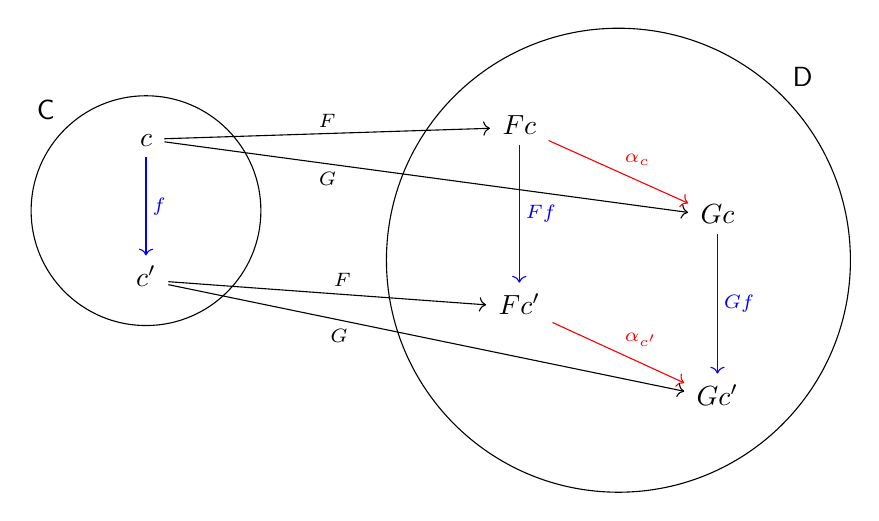
\begin{tikzpicture}[commutative diagrams/every diagram]
\matrix[matrix of math nodes, commutative diagrams/every cell] (mC) at (0,1.5) {c \\ \\ c' \\};
\path[commutative diagrams/.cd,every arrow,every label](mC-1-1)edge[blue] node {$f$}(mC-3-1);
\matrix[matrix of math nodes, commutative diagrams/every cell] (mD) at (6,0) {Fc &&  \\ && Gc \\ Fc'  && \\ && Gc' \\};
\path[commutative diagrams/.cd,every arrow,every label](mD-1-1)edge[red] node {$\alpha_c$}(mD-2-3);
\path[commutative diagrams/.cd,every arrow,every label] (mD-2-3) edge[blue] node {$Gf$} (mD-4-3);
\path[commutative diagrams/.cd,every arrow,every label](mD-3-1)edge[red] node {$\alpha_{c'}$}(mD-4-3);
\path[commutative diagrams/.cd,every arrow,every label](mD-1-1)edge[blue] node {$Ff$}(mD-3-1);

\path[commutative diagrams/.cd,every arrow,every label](mC-1-1)edge node {$F$}(mD-1-1);
\path[commutative diagrams/.cd,every arrow,every label](mC-1-1)edge[pos=0.34, swap] node {$G$}(mD-2-3);

\path[commutative diagrams/.cd,every arrow,every label](mC-3-1)edge node {$F$}(mD-3-1);
\path[commutative diagrams/.cd,every arrow,every label](mC-3-1)edge node[pos=0.36, swap] {$G$}(mD-4-3);

\node[draw=black,fit=(mC),circle, label={above left:$\cat{C}$}] (catC) {};
\node[draw=black,fit=(mD),circle, label={above right:$\cat{D}$}] (catD) {};
\end{tikzpicture}
\end{figure}
Thus a natural transformation is one that shifts the image of a functor along the morphisms in the target category.

This leads us to the following proposition, which is sometimes used to define natural transformations:
\begin{proposition}
Let $F,G:\cat{C}\to\cat{D}$ be functors. The natural transformations $\alpha: F\Rightarrow G$ correspond bijectively to functors $H: \cat{C}\times\mathbb{2}\to \cat{D}$ such that
\[ \begin{tikzcd}
\cat{C} \ar[r,"i_0"] \ar[dr, swap, "F"] & \cat{C}\times\mathbb{2} \ar[d,"H"] & \cat{C} \ar[l, swap, "i_1"] \ar[dl, "G"] \\
& \cat{D} &
\end{tikzcd} \qquad \text{commutes.} \]
Here $i_0, i_1$ are the functors that map objects $c$ to $(c,0)$ and $(c,1)$ respectively.

The same holds for natural isomorphisms, if $\mathbb{2}$ is replaced by $\mathbb{I}$.
\end{proposition}

\begin{example}
Let $M$ be a monoid. A \udef{dynamical system} is a functor $F: \cat{B}M\to\cat{C}$ from the delooping space to some category. Often this category is $\cat{Top}$ or $\cat{Vect}$. Then the single object of $\cat{B}M$ is mapped to an object $c$ in $\cat{C}$ and the morphisms of $\cat{B}M$ become actions on the object: each element $m\in M$ specifies a morphism in $\cat{B}M$, which is mapped to a morphism in $\cat{C}$
\[ m: c\to c: x\mapsto m\cdot x. \]

A morphism of dynamical systems, or \udef{intertwiner}, is a map between natural transformation $\alpha:F\to G$. This can be seen as a map between objects in $\cat{C}$ that is covariant, in the sense that
\[ \alpha(m\cdot x) = m\cdot \alpha(x). \]
\end{example}

\subsubsection{Natural transformations as canonical maps}
A canonical map $\alpha$ is a map between objects that arises naturally from the definition or the construction of the objects.

TODO: make rigourous! explicate for universal algebra.

In some sense the canonical map works at the level of structure and thus must commute with morphisms.

A \udef{canonical map} is a functor such that there exists a natural transformation from the identit functor to it.

TODO: what about between different categories?






\subsection{Equivalence of categories}
\begin{definition}
An \udef{equivalence of categories} consists of functors $F: \cat{C} \to \cat{D}$ and $G: \cat{D} \to \cat{C}$ such that we have natural isomorphisms $\id_\cat{C} \cong GF$ and $\id_\cat{D} \cong FG$.

The categories $\cat{C}, \cat{D}$ are \udef{equivalent} if there exists an equivalence between them. We write $\cat{C} \simeq \cat{D}$.
\end{definition}

Except for considerations of size, this equivalence is an equivalence relation.
\begin{lemma}
The notion of equivalence is reflexive, symmetric and transitive.
\end{lemma}



\begin{proposition}
A functor defining an equivalence of categories is full, faithful, and essentially surjective on objects.

Assuming the axiom of choice, any functor with these properties defines an equivalence of categories.
\end{proposition}


\begin{lemma}
An equivalence between skeletal categories is an isomorphism of categories
\end{lemma}
\begin{corollary}
Two categories are equivalent \textup{if and only if} their skeletons are isomorphic.
\end{corollary}

\begin{definition}
A category $\cat{C}$ is called
\begin{itemize}
\item \udef{essentially small} if it is equivalent to a small category (i.e.\ its skeleton is small);
\item \udef{essentially discrete} if it is equivalent to a discrete category (i.e.\ its skeleton is discrete).
\end{itemize}
\end{definition}

\begin{lemma}
Every preorder category is equivalent to a poset category.
\end{lemma}



\section{Monoidal categories}
\begin{definition}
A \udef{monoidal category} is a category $\cat{C}$ equipped with
\begin{enumerate}
\item a functor $\otimes: \cat{C}\times\cat{C} \to \cat{C}$ called the \udef{tensor product};
\item an object $1\in \cat{C}$ called the \udef{unit object} or the \udef{tensor unit}
\end{enumerate}
We write $(\cat{C}, \otimes, 1, \alpha, \lambda, \rho)$.
\end{definition}

\subsection{Enrichment}
\begin{definition}
Let $(\cat{V}, \otimes, 1, \alpha, \lambda, \rho)$ be a monoidal category. A \udef{$\cat{V}$-category} $\cat{C}$ (or \udef{$\cat{V}$-enriched category} or \udef{category enriched over $\cat{V}$}) contains
\begin{enumerate}
\item 
\end{enumerate}
such that
\end{definition}

\chapter{Object-free category theory}

\section{Categories as associative classes}
\subsection{Definition and identities}
\begin{definition}
Let $\cat{C}$ be an associative class. We call $\cat{C}$
\begin{itemize}
\item a \udef{left semi-category} if for all $x\in \cat{C}$, there exists
\begin{itemize}
\item a function $\dom: \cat{C}\to \cat{C}: x\mapsto 1_{\dom(x)}$, where $1_{\dom(x)}$ is a left identity such that $x1_{\dom(x)}$ exists; and
\item a function $\codom: \cat{C}\to \cat{C}: x\mapsto 1_{\codom(x)}$, where $1_{\codom(x)}$ is a left identity such that $1_{\codom(x)}x$ exists;
\end{itemize}
\item a \udef{category} if for all $x\in \cat{C}$, there exist identities $e,e'\in \cat{C}$ such that both $ex$ and $xe'$ are defined.
\end{itemize}
\end{definition}

An associative class that is both a left and right semi-category is a category (TODO make precise).

\begin{example}
The associative class of functions on sets is a left semi-category.
\end{example}

\begin{lemma} \label{categoryIdentities}
Let $\cat{C}$ be a category. Then
\begin{enumerate}
\item there exists a function $\dom: \cat{C}\to \cat{C}: x\mapsto 1_{\dom(x)}$, where $1_{\dom(x)}$ is the unique identity such that $x1_{\dom(x)}$ exists;
\item there exists a function $\codom: \cat{C}\to \cat{C}: x\mapsto 1_{\codom(x)}$, where $1_{\codom(x)}$ is the unique identity such that $\codom(x)x$ exists;
\item for all $x,y\in \cat{C}$: $xy$ is defined \textup{if and only if} $1_{\dom(x)} = 1_{\codom(y)}$.
\end{enumerate}
\end{lemma}
\begin{proof}
(1) and (2) are immediate. (We do not need choice due to the uniqueness, \ref{uniquenessIdentity})

(3) $\Rightarrow$ We have $xy = x1_{\dom(x)}1_{\codom(y)}y$,
so $1_{\dom(x)}1_{\codom(y)}$ is defined. Thus $1_{\dom(x)} = 1_{\codom(y)}$ by \ref{uniquenessIdentity}.

$\Leftarrow$ If $1_{\dom(x)} = e = 1_{\codom(y)}$, then $xe$ and $ey$ are defined, so $xey = xy$ is defined.
\end{proof}


\begin{lemma}
Let $\cat{C}$ be a category and $x,y\in \cat{C}$. Then
\begin{enumerate}
\item $1_{\dom(1_{\dom(x)})} = 1_{\dom(x)}$;
\item $1_{\codom(\codom(x))} = 1_{\codom(x)}$;
\item $1_{\dom(xy)} = 1_{\dom(y)}$;
\item $1_{\codom(xy)} = 1_{\codom(x)}$.
\end{enumerate}
\end{lemma}
\begin{proof}
(1) We have that $1_{\dom(1_{\dom(x)})}1_{\dom(x)}$ is defined by definition. As $1_{\dom(1_{\dom(x)})}$ and $1_{\dom(x)}$ are both identities, we have $1_{\dom(1_{\dom(x)})} = 1_{\dom(x)}$ from \ref{uniquenessIdentity}.

(2) Dual to (1).

(3) By definition, we have that
\[ (xy)1_{\dom(xy)} = x\big(y1_{\dom(xy)}\big) \]
is defined, so $y1_{\dom(xy)}$ is defined. As $1_{\dom(xy)}$ is an identity, it is equal to $1_{\dom(y)}$ by \ref{categoryIdentities}.
\end{proof}

\subsection{Left and right relations}
Diagrammatically,
\[ f \greensL g \quad\text{is equivalent to the commutativity of}\quad \begin{tikzcd}[row sep=small]
{} & B \arrow[dd, dashed, "a"] \\
A \arrow[ur, "f"] \arrow[dr, swap, "g"] & {} \\
{} & B' 
\end{tikzcd} \qquad \text{and}\qquad \begin{tikzcd}[row sep=small]
{} & B  \\
A \arrow[ur, "f"] \arrow[dr, swap, "g"] & {} \\
{} & B' \arrow[uu, dashed, "b"]
\end{tikzcd} \]
and
\[  f \greensR g \quad\text{is equivalent to the commutativity of}\quad \begin{tikzcd}[row sep=small]
A \arrow[dr, "f"] & {} \\
{} & B \\
A' \arrow[uu, dashed, "a"] \arrow[ur, swap, "g"] & {}
\end{tikzcd} \qquad \text{and}\qquad \begin{tikzcd}[row sep=small]
A \arrow[dd, dashed, "b"] \arrow[dr, "f"] & {} \\
{} & B \\
A' \arrow[ur, swap, "g"] & {}
\end{tikzcd}. \]



\begin{lemma} \label{leftRightRelatedIsomorphic}
Let $\cat{C}$ be a category and $f,g\in \cat{C}$.
\begin{enumerate}
\item If $f \greensL g$ and $f,g$ are epic, then $\codom(f) \cong \codom(g)$.
\item If $f \greensR g$ and $f,g$ are monic, then $\dom(f) \cong \dom(g)$.
\end{enumerate}
\end{lemma}
\begin{proof}
(1) Assume $f \greensL g$ and $f,g$ are epic. Set $A = \dom(f) = \dom(g)$, $B=\codom(f)$ and $B'=\codom(g)$. Then there exist $a,b\in \cat{C}$ such that
\[ \begin{tikzcd}[row sep=small]
{} & B \arrow[dd, shift left, "a"] \\
A \arrow[ur, "f"] \arrow[dr, swap, "g"] & {} \\
{} & B' \arrow[uu, shift left, "b"]
\end{tikzcd} \qquad \text{commutes with either only $a$ or only $b$ present.} \]
We need to show that the whole diagram commutes, for which we need to verify that $ba = 1_B$ and $ab = 1_{B'}$.

Indeed, $1_{B}f = f = bg = baf$, so $ba = 1_B$, and $1_{B'}g = af = abg$, so $ab = 1_{B'}$.

(2) Dual.
\end{proof}

\section{Functors}
\begin{definition}
A \udef{functor} is a homomorphism between associative classes.
\end{definition}

\section{Natural transformations}
\begin{definition}
Let $\sSet{A,\cdot}$ and $\sSet{B,\cdot}$ be associative classes. A \udef{natural transformation} $\alpha$ is a homomorphism $A\to B$ of two-sided algebras.
\end{definition}


\begin{definition}
Let $\sSet{A,\cdot}$ and $\sSet{B,\cdot}$ be associative classes. Let $F,G: A\to B$ be functors. A \udef{natural transformation} $\alpha$ from $F$ to $G$ is a function $\alpha: A\to B$ such that
\[ \forall f,g\in A: \qquad G(f)\alpha_g = \alpha_{fg} = \alpha_f F(g), \]
where we have written the arguments of $\alpha$ as subscripts: $\alpha_f$ means $\alpha(f)$.

We write $\alpha: F \Rightarrow G$.
\end{definition}

\subsection{Yoneda lemma}


\subsection{Operations with natural transformations}
\subsubsection{Vertical composition}
TODO: need define decomposable.
\begin{definition}
Let $A$ be an associative class that is decomposable. Let $B$ be anothor associative class.

Let $F,G,H: A\to B$ be functors and $\alpha: F\Rightarrow G$, $\beta: G\Rightarrow H$ natural transformations. The \udef{vertical composition} of $\alpha$ and $\beta$ is the natural transformation $\beta\circ\alpha: F\Rightarrow H$ defined by
$(\beta\circ\alpha)_{f} \defeq \beta_{f_2}\alpha_{f_1}$ if $f = f_2f_1$.
\end{definition}
Note that
\begin{itemize}
\item TODO: under what conditions is this well-defined???
\item $\beta\circ\alpha: F\Rightarrow H$ is a natural transformation from $F$ to $H$: $\forall f,g\in A$ we take $f = f_2f_1$, $g = g_2g_1$ and have
\[ H(f)(\beta\circ\alpha)_g = H(f_2)H(f_1)\beta_{g_2}\alpha_{g_1} =  \beta_{f_2}\alpha_{f_1}F(g_2)F(g_1) = (\beta\circ\alpha)_{f}F(g). \]
\end{itemize} 

\subsubsection{Whiskering}
\begin{definition}
Let $F,G: B\to C$ be functors and $\alpha: F\Rightarrow G$ a natural transformation.
\begin{itemize}
\item If $H: A\to B$ is a functor. Then the \udef{pre-whisker} of $H$ and $\alpha$ is the natural transformation $\alpha H: F\circ H\Rightarrow G\circ H$ defined by $(\alpha H)_f = \alpha_{H(f)}$.
\item If $H': C\to D$ is a functor. Then the \udef{post-whisker} of $H'$ and $\alpha$ is the natural transformation $H'\alpha: H'\circ F\Rightarrow H'\circ G$ defined by $(H'\alpha)_f = H'(\alpha_f)$.
\end{itemize}
\end{definition}
The pre-whisker of $H$ and $\alpha$ is a natural transformation $\alpha H: F\circ H\Rightarrow G\circ H$. Indeed, for all $f,g\in D$
\begin{align*}
(G\circ H)(f)(\alpha H)_g &= G\big(H(f)\big)\alpha_{H(g)} \\
&= \alpha_{H(f)}F\big(H(g)\big) \\
&= (\alpha H)_f(F\circ H)(g) .
\end{align*}
The post-whisker of $H'$ and $\alpha$ is also a natural transformation $H'\alpha: H'\circ F\Rightarrow H'\circ G$. Indeed, for all $f,g\in A$
\begin{align*}
(H'\circ G)(f)(H'\alpha)_g &= H'\big(G(f)\big)H'(\alpha_g) \\
&= H'\big(G(f)\alpha_g\big) \\
&= H'\big(\alpha_f F(g)\big) \\
&= H'(\alpha_f)H'\big(F(g)\big) \\
&= (H'\alpha)_f(H'\circ F)(g).
\end{align*}

Pictorially we can represent pre-whiskering as
\[ \begin{tikzcd}
A \arrow[r, "H"] & B \arrow[r, bend left=50, "F"{name=U}]
  \arrow[r, bend right=50, "G"{name=D, below}] & C \arrow[Rightarrow, from=U, to=D, shorten <=0.3em,shorten >=0.3em, "{\alpha}"]
\end{tikzcd} \qquad\text{becomes}\qquad \begin{tikzcd}[column sep=huge]
A \arrow[r, bend left=50, "F\circ H"{name=U}]
  \arrow[r, bend right=50, "G\circ H"{name=D, below}] & C \arrow[Rightarrow, from=U, to=D, shorten <=0.3em,shorten >=0.3em, "{\alpha H}"]
\end{tikzcd} \]
and post-whiskering as
\[ \begin{tikzcd}
B \arrow[r, bend left=50, "F"{name=U}]
  \arrow[r, bend right=50, "G"{name=D, below}] & C \arrow[Rightarrow, from=U, to=D, shorten <=0.3em,shorten >=0.3em, "{\alpha}"] \arrow[r, "{H'}"] & D
\end{tikzcd} \qquad\text{becomes}\qquad \begin{tikzcd}[column sep=huge]
B \arrow[r, bend left=50, "{H'\circ F}"{name=U}]
  \arrow[r, bend right=50, "{H'\circ G}"{name=D, below}] & D \arrow[Rightarrow, from=U, to=D, shorten <=0.3em,shorten >=0.3em, "{H'\alpha}"].
\end{tikzcd} \]

\subsubsection{Horizontal composition}
TODO

\subsection{Cones and limits}
\begin{definition}
Let $\sSet{J,\cdot}$ be an associative set and $\sSet{A,\cdot}$ an associative class. Let $F: J\to A$ be a diagram. Then
\begin{itemize}
\item a \udef{cone} over $F$ is a natural transformation $\alpha: C \Rightarrow F$ from a constant functor $C$ to $F$;
\item a \udef{cocone} under $F$ is a natural transformation $\beta: F\Rightarrow D$ from $F$ to a constant functor $D$.
\end{itemize}
We also define
\begin{itemize}
\item a \udef{limit} of the diagram $F: J\to A$ is a $[\setbuilder{\rho_a\circ -}{a\in A}]^!$-maximum in the class of cones over $F$.
\item a \udef{colimit} of the diagram $F: J\to A$ is a $[\setbuilder{\lambda_a\circ -}{a\in A}]^!$-maximum in the class of cocones over $F$.
\end{itemize}
\end{definition}

\begin{proposition}
Let $\cat{J}$ be a small category, $\cat{C}$ a category and $F: \cat{J}\to \cat{C}$ a (unital) diagram. Then the limits and colimits are categorical limits and colimits. In particular the image of the constant functor is an identity.
\end{proposition}
\begin{proof}
Universal property.
\end{proof}

\begin{proposition}
Let $\cat{J}$ be a small category and $\sSet{A,\cdot}$ an associative class. Let $F: \cat{J}\to A$ be a diagram and $\alpha: C\Rightarrow F$ a limit of $F$. Then
\begin{enumerate}
\item the single element $c$ of $\im(C)$ is idempotent and the unique element of $a$ such that $\alpha_- = \alpha_-c$;
\item if $f,g\in A$ are such that $fg$ exists, then $\alpha_f = F(f)\alpha_g$.
\end{enumerate}
\end{proposition}
\begin{proof}
(1) As $\cat{J}$ is a category, it contains an idempotent $e$. Then $c = C(e) = C(e^2) = C(e)C(e) = c^2$, so $c$ is also idempotent.

For all $f:A\to B\in \cat{J}$, we have $\alpha_f = \alpha_{f\id_A} = \alpha_f C(\id_A) = \alpha_f c$.

The uniqueness follows by definition.

(2) We have $\alpha_f = \alpha_fc = \alpha_f C(g) = F(f)\alpha_g$.
\end{proof}

The limit is uniquely determined by its components at sources!

\chapter{Higher category theory}
\section{2-categories}
\subsection{Functor categories}
\begin{proposition} \label{functorCategory}
Let $\cat{C}, \cat{D}$ be categories. There is a category of functors $\cat{C}\to \cat{D}$ with as morphisms natural transformations called the \udef{functor category} $[\cat{C},\cat{D}]$.
\end{proposition}
\begin{proof}
There are clearly identity natural transformations $I:F\Rightarrow F$ for each functor $F: \cat{C}\to \cat{D}$ with components given by $I_{Fc}$ for all $c\in\cat{C}$.

To verify composition, let $\alpha: F \Rightarrow G$ and $\beta: G\Rightarrow H$ be natural transformations between parallel functors $F,G,H: \cat{C}\to \cat{D}$. Then the composition	$\beta\alpha: F\Rightarrow H$ has components
\[ (\beta\alpha)_c = \beta_c\alpha_c. \]
We just need to show $\beta\alpha$ is a natural transformation. Consider the diagram
\[ \begin{tikzcd}
Fc \ar[r, "\alpha_c"] \ar[d, "Ff"] & Gc \ar[d, "Gf"] \ar[r, "\beta_c"] & Hc \ar[d,"Hf"] \\
Fc' \ar[r, "{\alpha_{c'}}"] & Gc' \ar[r, "{\beta_{c'}}"] & Hc'
\end{tikzcd} \]
Both squares commute by naturality of $\alpha,\beta$. The rectangle then commutes: the only non-trivial part is the equality of paths $Fc\to Hc'$, but any such path can be deformed into another by flipping over squares (TODO better reference).
\end{proof}

\subsection{The 2-category of categories}


\chapter{Representability and universal properties}
\section{The Yoneda lemma}
\url{https://math.stackexchange.com/questions/149376/excessive-use-of-the-yoneda-lemma}
\url{https://qchu.wordpress.com/2012/04/02/the-yoneda-lemma-i/}
\begin{lemma}
Let $\cat{C},\cat{D}$ be categories. For every $c\in\cat{C}$, there is a functor defined by
\[ \evalMap_c: [\cat{C},\cat{D}] \to \cat{D}: F\mapsto Fc. \]
\end{lemma}
\begin{proof}
A natural transformation $\alpha: F \Rightarrow G$ is mapped to its component $\alpha_c: Fc \to Gc$. By \ref{functorCategory}, for all $F$, $I_F\mapsto I_{Fc}$ and the composition of composable natural transformations $\beta,\alpha$ has the component $\beta_c\alpha_c$ at $c$.
\end{proof}
So this gives us a functor
\[ \evalMap: (\cat{Set^C}, \cat{C}) \to \cat{Set}: \quad (F,c)\mapsto Fc.\]

Let $\cat{C}$ be a small category. Then for a given $c\in\cat{C}$, $\cat{C}(c,-)$ is the covariant functor represented by $c$ and thus an object in $[\cat{C},\cat{\Set}]$, which is locally small. Then we can consider the covariant functor represented by $\cat{C}(c,-)$,
\[ [\cat{C},\cat{\Set}]\to \cat{Set}:\quad F \mapsto \Hom(\cat{C}(c,-), F). \]

By currying, we can consider the two-sided represented functor $\cat{C}(-,-): \cat{C^{op}}\times\cat{C}\to \cat{Set}$ as a contravariant functor $\cat{C} \to \cat{Set^C}: c\mapsto \cat{C}(c,-)$. Composing this with the contravariant functor represented by $F$ gives the covariant functor
\[ \cat{C} \to \cat{Set}:\quad c \mapsto \Hom(\cat{C}(c,-), F). \]

Combining these two functors we have a bifunctor
\[ (\cat{Set^C}, \cat{C}) \to \cat{Set}: \quad(F,c) \mapsto \Hom(\cat{C}(c,-), F). \]

If we now let $\cat{C}$ be only locally small, not necessarily small, $\cat{Set^C}$ is no longer necessarily locally small. It turns out however that $\Hom(\cat{C}(c,-), F)$ still always yields a set. This assertion is part of the Yoneda lemma. The other part is the assertion that there is a natural isomorphism $\Phi$:
\[ \begin{tikzcd}
\cat{C}\times\cat{Set^C} \ar[rr, bend left=50, "{\Hom(\cat{C}(c,-), F)}"] \ar[rr, bend right=50, "\evalMap_c(F)"] & \Phi\Downarrow\cong & \cat{Set}
\end{tikzcd}. \]

\begin{theorem}[Yoneda lemma] \label{YonedaLemma}
Let $\cat{C}$ be a locally small category.

Given a functor $F: \cat{C} \to \cat{Set}$ and an object $c$ in $\cat{C}$, the function
\[ \Phi_{c,F}: \Hom(\cat{C}(c,-), F) \to Fc: \alpha \mapsto \alpha_c(I_c) \]
is a bijection.

Also $\Phi$ is a natural transformation with components $\Phi_{c,F}$.
\end{theorem}
\begin{corollary}[Yoneda embedding] \label{YonedaEmbedding}
Let $\cat{C}$ be a locally small category. The functors
\[ \begin{tikzcd}
\cat{C} \ar[r, hook] & \cat{Set^{C^{op}}} \\
c \ar[d, swap, "f"]\ar[r, mapsto] \ar[r,mapsto, shift right=1.7em] & \cat{C}(o(-),c) \ar[d, "f_*"] \\
d \ar[r,mapsto] & \cat{C}(o(-),d)
\end{tikzcd} \qquad\text{and}\qquad \begin{tikzcd}
\cat{C^{op}} \ar[r, hook] & \cat{Set^C} \\
c \ar[r, mapsto] \ar[r,mapsto, shift right=1.7em] & \cat{C}(c,-) \\
d \ar[u, "f^o"] \ar[r,mapsto] & \cat{C}(d,-) \ar[u, swap, "f^*"]
\end{tikzcd} \]
define full and faithful embeddings.
\end{corollary}
\begin{proof}
The functors are clearly injective on objects as morphisms with different domain or codomain are different.

Consider first the left embedding. We want the transformation $f_*$ to be natural (this is the transformation with all components equal to $f_*$). Indeed the functors $\cat{C}(o(-),c)$ and $\cat{C}(o(-),c)$ map morphisms $g^o$ in $\cat{C^{op}}$ to $g^*$. Now $f_*$ and $g^*$ clearly commute, proving the naturality of $f_*$.

Then the function $\cat{C}(c,d) \to \Hom(\cat{C}(-,c),\cat{C}(-,d)): f\mapsto f_*$ is the inverse of the Yoneda map $\Phi_{c,\cat{C}(-,d)}$:
\[ \Phi_{c,\cat{C}(-,d)}(f_*) = f_*(I_c) = f\circ I_c = f. \]
Thus by the Yoneda lemma it is bijection, meaning
\[ \cat{C}(c,d) \cong \Hom(\cat{C}(-,c),\cat{C}(-,d)) \]
and the left functor is full and faithful by definition.

The statement for the right functor can be proven analogously. Alternatively, we can see that it is a dual statement in the following way: taking the category to be $\cat{C^{op}}$, we get
\[ \cat{C^{op}}(c,d) \cong \Hom(\cat{C^{op}}(-,c),\cat{C^{op}}(-,d)) \]
or
\[ o[\cat{C}(d,c)] \cong \Hom(o\cdot\cat{C}(c,-)\cdot o,o\cdot\cat{C}(d,-)\cdot o) \]
now for every $\alpha \in \Hom(\cat{C}(c,-),\cat{C}(d,-))$, there is an $\alpha^o$ in $\Hom(o\cdot\cat{C}(c,-)\cdot o,o\cdot\cat{C}(d,-)\cdot o)$, so we have an isomorphism
\[ \cat{C}(d,c) \cong \Hom(\cat{C}(c,-),\cat{C}(d,-)). \]
\end{proof}

It is common to refer both to the Yoneda lemma \ref{YonedaLemma} and its corollary on the Yoneda embedding, \ref{YonedaEmbedding}, as the Yoneda lemma.

\begin{proposition} \label{representablyIsomorphic}
Let $\cat{C}$ be a locally small category. The following are equivalent:
\begin{enumerate}
\item $f:x\to y$ is an isomorphism in $\cat{C}$;
\item $f_*: \cat{C}(-,x) \Rightarrow \cat{C}(-,y)$ is a natural isomorphism;
\item $f^*: \cat{C}(y,-) \Rightarrow \cat{C}(x,-)$ is a natural isomorphism.
\end{enumerate}
\end{proposition}
\begin{proof}
We have already shown $f_*$ and $f^*$ are natural transformations in \ref{YonedaEmbedding}.
The proof follows from the Yoneda embedding \ref{YonedaEmbedding} and \ref{isomorphismCreationReflection}.

Alternatively, a partial proof is as follows: If $f$ has an inverse $f^{-1}$, then $(f^{-1})^*$ is an inverse of $f^*$ and $(f^{-1})_*$ an inverse of $f_*$.
\end{proof}

\section{Representable functors}
\subsection{Functors represented by objects}
\begin{definition}
Let $\cat{C}$ be a locally small category and $c$ an object in $\cat{C}$.

Given a morphism $f: X\to Y$ in $\cat{C}$, we can define the functions
\begin{enumerate}
\item $f_*: \cat{C}(c,X) \to \cat{C}(c,Y): g\mapsto fg$ defined by post-composition;
\item $f^*: \cat{C}(Y,c) \to \cat{C}(X,c): g\mapsto gf$ defined by pre-composition.
\end{enumerate}
These are morphisms in the category $\cat{Set}$.

Based on this we can define the \udef{covariant functor represented by $c$} $\cat{C}(c,-)$ and the \udef{contravariant functor represented by $c$} $\cat{C}(-,c)$:
\[ \begin{tikzcd}
\cat{C} \ar[r, "{\cat{C}(c,-)}"] & \cat{Set} \\
x \ar[d, swap, "f"]\ar[r, mapsto] \ar[r,mapsto, shift right=1.7em] & \cat{C}(c,x) \ar[d, "f_*"] \\
y \ar[r,mapsto] & \cat{C}(c,y)
\end{tikzcd} \qquad\qquad \begin{tikzcd}
\cat{C} \ar[r, "{\cat{C}(-,c)}"] & \cat{Set} \\
x \ar[r, mapsto] \ar[r,mapsto, shift right=1.7em] & \cat{C}(x,c) \ar[d, "f^*"] \\
y \ar[u, "f"] \ar[r,mapsto] & \cat{C}(y,c) 
\end{tikzcd} \]
We also have the \udef{two-sided represented functor} $\cat{C}(-,-):\cat{C}\times \cat{C} \to \cat{Set}$, which is contravariant in the first argument and covariant in the second:
\[ \begin{tikzcd}
\cat{C}\times\cat{C} \ar[r, "{\cat{C}(-,-)}"] & \cat{Set} \\
(x,y) \ar[d, shift left]\ar[r, mapsto] \ar[r,mapsto, shift right=1.7em] & \cat{C}(x,y) \ar[d, "{f^*h_*: g\mapsto hgf}"] \\
(w,z) \ar[u, shift left, "{(f,h)}"] \ar[r,mapsto] & \cat{C}(w,z)
\end{tikzcd} \]
\end{definition}
The placement of the asterisk indicates the placement of the function being composed with $f$: below means to the right and above to the left. This is consistent with the notation for indicating bases in the part on matrix representations of linear functions (TODO ref).

\begin{proposition}
Let $\cat{C}$ be a locally small category and $f: X\to Y$ a morphism. Then $f_*$ and $f^*$ are dual as follows:
\begin{align*}
(f^\text{o})^* &= of_*o = (f^*)^o; \\
(f^\text{o})_* &= of^*o = (f^*)^o.
\end{align*}
\end{proposition}
\begin{proof}
We start with the locally small category $\cat{C^{op}}$, the morphism $f^\text{o}: Y\to X$ and an object $c$. Then 
\[ (f^\text{o})^*: \cat{C^{op}}(X,c) \to \cat{C^{op}}(Y,c): g^\text{o} \mapsto g^\text{o}f^\text{o}. \]
We can rewrite this as
\[ (f^\text{o})^*: o[\cat{C}(c,X)] \to o[\cat{C}(c,Y)]: g^o \mapsto (fg)^o \]
or
\[ o|_{o[\cat{C}(Y,c)]}(f^\text{o})^*o|_{\cat{C}(c, X)}: \cat{C}(c,X) \to \cat{C}(c,Y): g \mapsto fg. \]
This last function is exactly $f_*$. The other equality follows by duality: replacing $\cat{C}$ with $\cat{C^{op}}$ and $f: X\to Y$ with $f^o: Y\to X$ gives
\[ (f^o)_* = o|_{o[\cat{C^{op}}(X,c)]}(f^\text{oo})^*o|_{\cat{C^{op}}(c, Y)} = o|_{\cat{C}(c,X)}f^*o|_{o[\cat{C}(Y,c)]} \]
so
\[ f^* =  o|_{o[\cat{C}(c,X)]}(f^o)_* o|_{\cat{C}(Y,c)}. \]
\end{proof}
\begin{corollary} \label{dualityRepresentedFunctors}
The co- and contravariant represented functors are dual in the following sense:
\begin{align*}
o\cdot \cat{C^{op}}(c,-) \cdot o &= \cat{C}(-,c) \\
o\cdot \cat{C^{op}}(-,c) \cdot o &= \cat{C}(c,-) \\
\end{align*}
\end{corollary}
Note that $o$ still works as a function on sets of morphisms in $\cat{C}$, even though they are now said to be in the category $\cat{Set}$. We also use that $o$ acts on transformations as $o(\alpha) = o\alpha o$ (TODO!).
\begin{proof}
We verify the equality for all objects and morphisms:
\[ (o\cdot \cat{C^{op}}(c,-) \cdot o)(x) = (o\cdot \cat{C^{op}}(c,-))(x) = o(\cat{C^{op}}(c,x)) = o(o(\cat{C}(x,c))) = \cat{C}(x,c) \]
and
\[ (o\cdot \cat{C^{op}}(c,-) \cdot o)(f) = (o\cdot \cat{C^{op}}(c,-))(f^o) = o((f^o)_*) =o(of^*o) = oof^*oo = f^*. \]
\end{proof}

\begin{proposition} \label{monicEpicInPrePostComposition}
Let $\cat{C}$ be a locally small category and $f: X\to Y$ a morphism. Then
\begin{enumerate}
\item $f: X\to Y$ is monic \textup{if and only if} for all $c$ in $\cat{C}$, $f_*: \cat{C}(c,X) \to \cat{C}(c,Y)$ is injective;
\end{enumerate}
and, dually,
\begin{enumerate}
\setcounter{enumi}{1}
\item $f:X\to Y$ is epic \textup{if and only if} for all $c$ in $\cat{C}$, $f^*: \cat{C}(Y,c) \to \cat{C}(X,c)$ is injective.
\end{enumerate}
\end{proposition}
\begin{proof}
Assume $f$ monic. To show injectivity, assume $f_*(g) = f_*(h)$, which means $fg = fh$. By monicity $g = h$, showing $f^*$ is injective.

The converse is equally direct, as is the second statement.

The second statement also follows by duality, recognising that because $o$ is bijective when restricted to the relevant sets, $of^*o$ is injective if and only if $f^*$ is, by \ref{injectiveMonoSurjectiveEpi} and \ref{monicEpicCompositions}.
\end{proof}

\subsection{Representable functors}
\begin{definition}
Let $\cat{C}$ be a locally small category.

A covariant / contravariant functor $F: \cat{C} \to \cat{Set}$ is \udef{representable} if there is an object $c\in\cat{C}$ such that $F$ is naturally isomorphic to the covariant / contravariant functor represented by $c$, i.e.\
\[ F \cong \begin{cases}
\cat{C}(c,-) & \text{$F$ covariant} \\
\cat{C}(-,c) & \text{$F$ contravariant.}
\end{cases} \]
We say $F$ is \udef{represented} by the object $c\in\cat{C}$.

A \udef{representation} of a functor $F: \cat{C} \to \cat{Set}$ is given by an object $c\in\cat{C}$ and a natural isomorphism $\alpha$ from $F$ to the functor represented by $c$.
\end{definition}
A functor is represented by at most one object, up to isomorphism, by \ref{representablyIsomorphic}.

By the Yoneda lemma, every natural isomorphism $\alpha$ corresponds to en element $\alpha_c(I_c) \in Fc$.
\begin{definition}
A \udef{univeral property} of an object $c\in \cat{C}$ is expressed by a representable functor $F$ together with a \udef{universal element} $x\in Fc$ that corresponds to a natural isomorphism between $F$ and the functor represented by $c$.
\end{definition}
\section{The category of elements}
\chapter{Cones and cocones}

\section{Cone and leg categories}
\begin{proposition}
Cone (and leg) categories are preserved under commuting extensions (with arrows outwards!!) of the diagram.
\end{proposition}

\begin{proposition}
Cone category is intersection \emph{of objects} in leg categories.
\end{proposition}
Note that we do not need to check commuting properties.

\begin{corollary}
Given two diagrams such that there exists a commuting canonical extension diagram that encompasses both, then the (co)cone categories of all three diagrams are the same.
\end{corollary}

\section{Finite limits}
\subsection{Product}
TODO: use $\prod$?? TODO use $\pi$. TODO proofs

\[ \begin{tikzcd}
& X \arrow[d, dashed, near end, "{(f,g)}"] \arrow[dl, swap, "f"] \arrow[dr, "g"] & \\
A & A\times B \arrow[l, "{\pi_A}"] \arrow[r, swap, "{\pi_B}"] & B
\end{tikzcd} \]

We denote the unique morphism $(f,g)$.

\begin{definition}
Let $A$ be an object, then we define
\begin{itemize}
\item the \udef{square} of $A$ as $A^2 \defeq A\times A$;
\item the \udef{diagonal map} on $A$ as $\delta_A = (\id_A, \id_A): A\to A^2$.
\end{itemize}
Let $h: A\to X$ and $k: B\to Y$ be morphisms. Then we define $(h|k): A\times B\to X\times Y$ as $(h|k) \defeq (h\circ\pi_1, k\circ\pi_2)$.
\end{definition}

\begin{lemma} \label{compositionProjectionMorphisms}
Let $\begin{tikzcd}[row sep=-0.7em, column sep=1em]
&& A \\
X \ar[r, "h"] & Y \ar[ur, "f"] \ar[dr, swap, "g"] & \\
&& B
\end{tikzcd}$ be morphisms in a category $\cat{C}$ which contains $A\times B$.

Then
$\begin{tikzcd}
X \ar[r, "h"] \ar[rr, bend left, "{(f\circ h,g \circ h)}"] & Y \ar[r, "{(f,g)}"] & A\times B
\end{tikzcd}$ commutes.
In other words: $(f,g)\circ h = (f\circ h, g\circ h)$.
\end{lemma}

\begin{lemma} \label{productFactorisationMorphisms}
Let $X,A,B$ be morphism in a category $\cat{C}$ such that $A\times B$ exists. Let $f: X\to A\times B$,  $g: X\to A$ and $g': X\to B$ be morphisms. Then
\begin{enumerate}
\item $f = (\proj_A\circ f, \proj_B\circ f)$;
\item $g = \pi_A\circ(g,g')$ and $g' = \pi_B\circ(g,g')$.
\end{enumerate}
\end{lemma}

\begin{lemma}
Let $A,B$ be objects in a category $\cat{C}$. Then there exists an isomorphism $A\times B \to B\times A$.
\end{lemma}

\begin{lemma} \label{parallelCompositionOfMorphisms}
Let $f: A\to X, g: B\to Y, h: X\to U$ and $k: Y\to V$ be morphisms. Then $(h|k)\circ (f|g) = (h\circ f | k\circ g)$.
\end{lemma}
\begin{proof}
We calculate, using \ref{productFactorisationMorphisms},
\begin{align*}
(h|k)\circ (f|g) &= (h\circ \pi_1, k\circ\pi_2) \circ (f\circ \pi_1, g\circ\pi_2) \\
&= \big(h\circ \pi_1\circ (f\circ \pi_1, g\circ\pi_2), k\circ\pi_2\circ (f\circ \pi_1, g\circ\pi_2)\big) \\
&= (h\circ f\circ \pi_1, k\circ g\circ\pi_2) \\
&= (h\circ f | k\circ g).
\end{align*}
\end{proof}

\begin{lemma}
Let $A$ be an object in a category $\cat{C}$ with terminal object $1$. Then $A \cong A\times 1$.
\end{lemma}


\begin{proposition} \label{associatorTernaryProducts}
Let $\cat{C}$ be a category with binary products and $A,B,C$ objects in this category. Then there exists a unique isomorphism
\[ (A\times B)\times C \to A\times (B\times C). \]
\end{proposition}
\begin{proof}
Both $(A\times B)\times C$ and $A\times (B\times C)$ are limits of the diagram $\begin{tikzcd}
A & B & C
\end{tikzcd}$.
\end{proof}

\subsection{Equalisers and coequalisers}
\begin{definition}
Consider the category $\mathbb{D}: \begin{tikzcd}
\bullet \ar[loop left] \ar[r, shift left] \ar[r, shift right] & \bullet \ar[loop right]
\end{tikzcd}$ and let $\cat{C}$ be some other category. An \udef{equaliser} in $\cat{C}$ is the limit of a $\mathbb{D}$-diagram in $\cat{C}$.

A \udef{coequaliser} in $\cat{C}$ is the colimit of a $\mathbb{D}$-diagram in $\cat{C}$.
\end{definition}

\begin{lemma}
Let $\cat{C}$ be a category and $f,g: A\to B$ morphisms in $\cat{C}$ with equaliser
\[ \begin{tikzcd}[column sep=tiny]
& E \ar[dl, swap, "e"] \ar[dr, "{e'}"] & \\
A \ar[rr, shift left, "f"] \ar[rr, shift right, swap, "g"] && B
\end{tikzcd} \]
Then the leg $E\to B$ is redundant.
\end{lemma}
In other words, the morphism $e: E\to A$ determines the equaliser \textup{if and only if} $\forall h: X\to A$ such that $fh = gh$:
\[ \exists! \theta : \qquad \begin{tikzcd}
X \ar[d, dashed, swap, "{\exists! \theta}"] \ar[dr, "h"] && \\
E \ar[r, "e"] & A \ar[r, shift left, "f"] \ar[r, shift right, swap, "g"] & B
\end{tikzcd} \qquad \text{commutes.} \]
\begin{proof}
Clearly $e'$ is uniquely determined by $e$: because the diagram commutes, we have $e' = f\circ e = g\circ e$.

If $e: E\to A$ has the property, then defining $e' = f\circ e = g\circ e$, makes $(e,e')$ a limit. TODO redundant legs.
\end{proof}

\begin{lemma} \label{equaliserMonic}
Let $\cat{C}$ be a category and $f,g: A\to B$ morphisms. If the equaliser $e: E\to A$ exists, it is monic.
\end{lemma}
\begin{proof}
Take arbitrary $h_1, h_2: X\to E$ such that $e\circ h_1 = e\circ h_2$. Then consider the diagram
\[ \begin{tikzcd}
X \ar[d, dashed, swap, "h"] \ar[dr, "{e\circ h_1 = e\circ h_2}"] && \\
E \ar[r, "e"] & A \ar[r, shift left, "f"] \ar[r, shift right, swap, "g"] & B
\end{tikzcd} \]
which commutes if $h = h_1$ or $h = h_2$. But, because $e$ is the equaliser, there may exist only one $h$ that makes the diagram commute, so $h_1 = h_2 = h$.
\end{proof}

\subsubsection{Kernels and cokernels}
\begin{definition}
Let $\cat{C}$ be a category with zero morphisms and $f:A\to B$ a morphism.
\begin{itemize}
\item The \udef{kernel} of $f$ is the equaliser of $f$ and the zero morphism $0:A\to B$.
\item The \udef{cokernel} of $f$ is the coequaliser of $f$ and the zero morphism $0:A\to B$.
\end{itemize}
\end{definition}

\begin{proposition} \label{epicMonicZeroKernelCokernel}
Let $\cat{C}$ be a category with a zero object $0$ and $f:A\to B$ a morphism. Then
\begin{enumerate}
\item if $f$ is monic, then $0_{0,A}\in \ker(f)$;
\item if $f$ is epic, then $0_{0,A}\in \coker(f)$.
\end{enumerate}
\end{proposition}
\begin{proof}
(1) We have $f0_{0,A} = 0_{0,B} = 0_{A,B}0_{0,A}$, so $0_{0,A}$ determines a cone over the diagram $\begin{tikzcd}
A \arrow[r, shift left, "f"] \arrow[r, shift right, swap, "{0_{A,B}}"] & B
\end{tikzcd}$. For any other cone $h: A'\to A$, we have a unique morphism from $A'$ to $0$. In order to prove that $0_{0,A}\in\ker(f)$, we need to show that the diagram
\[ \begin{tikzcd}
A' \ar[d, swap, "{0_{A', 0}}"] \ar[dr, "h"] && \\
0 \ar[r, "0_{0,A}"] & A \ar[r, shift left, "f"] \ar[r, shift right, swap, "{0_{A,B}}"] & B
\end{tikzcd}\qquad\text{commutes.} \]
The only part that remains to be proven is that $h = 0_{0,A}0_{A',0}$. We have
\[ fh = 0_{A,B}h = 0_{A',B} = 0_{A,B}0_{0,A}0_{A',0} = f0_{0,A}0_{A',0}. \]
As $f$ is monic, the equality $fh = f0_{0,A}0_{A',0}$ implies $h = 0_{0,A}0_{A',0}$.

(2) Dual.
\end{proof}
TODO: opposite implication for additive categories (??)

\begin{lemma} \label{identityAsKernelCokernel}
Let $\cat{C}$ be a category with zero element and $A\in\ob(\cat{C})$. Then
\begin{enumerate}
\item $1_A \in \ker(A\to 0)$;
\item $1_A \in \coker(0\to A)$.
\end{enumerate} 
\end{lemma}

\subsection{Pullbacks}
\begin{definition}

\end{definition}

\begin{lemma} \label{productAsPullback}
Let $\cat{C}$ be a category with terminal object $T$ and $A,B\in\ob(\cat{C})$. Then $A\times B = A\times_T B$.
\end{lemma}
\begin{proof}
The cocone categories of
\[ \begin{tikzcd}
A & B
\end{tikzcd} \qquad\text{and}\qquad \begin{tikzcd}
A \ar[r] & T & \ar[l] B
\end{tikzcd} \]
are the same.
\end{proof}


\subsection{Implications regarding existence}

\begin{proposition}
Let $\cat{C}$ be a category. The following are sufficient conditions for the existence of equalisers in $\cat{C}$:
\begin{enumerate}
\item the existence of pullbacks (of a morphism and a monomorphism) and squares;
\item the existence of pullbacks of two monomorphism and products;
\item the existence of pullbacks and a terminal object.
\end{enumerate}
\end{proposition}
\begin{proof}
Let $f,g: A\to B$ be morphisms in $\cat{C}$.

(1) The equaliser of $f,g$ is the pullback
\[ \begin{tikzcd}
E \arrow[r] \arrow[d, "e"] \pbCorner & B \arrow[d, "{\delta_B}"] \\
A \arrow[r, swap, "{(f,g)}"] & B^2
\end{tikzcd} \]
because the diagrams $\begin{tikzcd}
A \ar[r, shift left, "f"] \ar[r, shift right, swap, "g"] & B
\end{tikzcd}$ and $\begin{tikzcd}
A \ar[r, "{(f,g)}"] & B^2 & \ar[l, swap, "{\delta_B}"] B
\end{tikzcd}$ are contained in the commuting diagram
\[ \begin{tikzcd}[column sep=large]
& B \ar[dr, leftrightarrow, "{\id_B}"] & \\
A \ar[r, pos=0.6, "{(f,g)}"] \ar[ur, "f"] \ar[dr, swap, "g"] & B^2 & \ar[l, swap, "{\delta_B}"] B \\
& B \ar[ur,swap, leftrightarrow, "{\id_B}"] &
\end{tikzcd} \]
(TODO: work out formalism!!)

(2) The equaliser of $f,g$ is the pullback
\[ \begin{tikzcd}
E \arrow[r] \arrow[d, "e"] \pbCorner & A \arrow[d, "{(\id_A, f)}"] \\
A \arrow[r, swap, "{(\id_A,g)}"] & A\times B
\end{tikzcd} \]
because the diagrams $\begin{tikzcd}
A \ar[r, shift left, "f"] \ar[r, shift right, swap, "g"] & B
\end{tikzcd}$ and $\begin{tikzcd}
A \ar[r, "{(\id_A,g)}"] & A\times B & \ar[l, swap, "{(\id_A, f)}"] B
\end{tikzcd}$ are contained in the commuting diagram
\[ \begin{tikzcd}[column sep=large]
& A \ar[dr, "{f}"] \ar[d, swap, pos=0.7, "{(\id_A, f)}"] & \\
A \ar[ur, leftrightarrow, "{\id_A}"] \ar[dr, leftrightarrow, swap, "{\id_A}"] & A\times B \ar[r, "{\proj_B}"] & B \\
& A \ar[ur, swap, "{g}"] \ar[u, pos=0.7, "{(\id_A, g)}"] &
\end{tikzcd} \]
(TODO: work out formalism!!)

(3) From point (2) and \ref{productAsPullback}.
\end{proof}

\begin{lemma}

\end{lemma}

\begin{proposition}
Let $\cat{C}$ be a category. If products and equalisers exist, then all finite limits exist.
\end{proposition}
Note that we assume all products exist, including products of zero factors (i.e.\ terminal objects).
\begin{proof}
Take product over all objects in diagram and the equalise over all paths that need to be the same in order for the cone to commute properly.

TODO: Show that multiple equalisation commutes.
\end{proof}
\begin{corollary} \label{productsMonicPullbacksComplete}
Let $\cat{C}$ be a category. If products and pullbacks of monomorphisms exist, then all finite limits exist.
\end{corollary}

\begin{example}
For the existence of pullbacks:

Let $f: A_1 \to B$ and $g: A_2 \to B$ be morphisms. Then the pullback of $\begin{tikzcd}
A_1 \ar[r, "f"] & B & \ar[l, swap, "g"] A_2
\end{tikzcd}$ is the equaliser of
\[ \begin{tikzcd}
& A_1 \times A_2 \ar[dl, swap, "\proj_1"] \ar[dr, "\proj_2"] & \\
A_1 \ar[r, "f"] & B & \ar[l, swap, "g"] A_2
\end{tikzcd} \]
(TODO formalism)

\end{example}

\section{Finite colimits}
\subsection{Coproducts}

We denote the unique morphism $(f \bbslash g)$.

\section{Infinite limits and colimits}
\subsection{Projective (or inverse) limit}
\begin{definition}
Let $\sSet{I, \preceq}$ be a reflexive upwards directed set and $\cat{C}$ a category. Let $X_i$ be an object in $\cat{C}$ for all $i\in I$ and let $p_{j,i}: X_j \to X_i$ be a morphism in $\cat{C}$ for all $i \preceq j$ such that
\begin{itemize}
\item $p_{i,i} = \id_{X_i}$ for all $i\in I$;
\item $p_{k,i} = p_{k,j}; p_{j,i} = p_{j,i}\circ p_{k,j}$ for all $i\preceq j \preceq k$.
\end{itemize}
Then the structure $\sSet{I, \{X_i\}_{i\in I}, \{p_{j,i}\}_{i\preceq j}}$ is called a \udef{projective system} (or \udef{inverse system}).

A limit of the diagram
\[ \begin{tikzcd}
{}&{}&{}&{}&{} \\
\hdots \ar[r] & X_k \ar[dr]\ar[ur] \ar[r, "p_{k,j}"]  & X_j \ar[dr]\ar[ur]\ar[r, "p_{j,i}"] & X_i \ar[r]\ar[dr]\ar[ur] & \hdots \\
{}&{}&{}&{}&{}\\
\end{tikzcd} \]
is called a \udef{projective limit} (or \udef{inverse limit}) and is denoted $X=\varprojlim _{i\in I}{X_{i}}$.
\end{definition}
In other words, we have a projective system if the diagram
\[ \begin{tikzcd}[column sep=large]
X_k \ar[rr, "p_{k,i}"] \ar[rd, "p_{k,j}"] & & X_i \\
& X_j \ar[ur, "p_{j,i}"]
\end{tikzcd} \qquad \text{commutes for all $i\preceq j \preceq k$.} \]

TODO: definition using contravariant functor $I\to \cat{C}$.

\begin{proposition}
In the category $\cat{Set}$ the projective limit of each projective system $\sSet{I, \{X_i\}_{i\in I}, \{p_{j,i}\}_{i\preceq j}}$ exists and is given by
\[ \varprojlim _{i\in I}{X_{i}}=\setbuilder{a\in \prod _{i\in I}A_{i}}{\forall i\preceq j:\; \pi_i(a) = p_{j,i}\big(\pi_j(a)\big)}. \]
\end{proposition}
Compare with constructions in infinitely complete categories.

\subsection{Inductive (or direct) colimit}
\begin{definition}
Let $\sSet{I, \preceq}$ be a reflexive upwards directed set and $\cat{C}$ a category. Let $X_i$ be an object in $\cat{C}$ for all $i\in I$ and let $e_{i,j}: X_i \to X_j$ be a morphism in $\cat{C}$ for all $i \preceq j$ such that
\begin{itemize}
\item $e_{i,i} = \id_{X_i}$ for all $i\in I$;
\item $e_{i,k} = e_{i,j}; e_{j,k} = e_{j,k}\circ e_{i,j}$ for all $i\preceq j \preceq k$.
\end{itemize}
Then the structure $\sSet{I, \{X_i\}_{i\in I}, \{e_{i,j}\}_{i\preceq j}}$ is called an \udef{inductive system} (or \udef{direct system}).

A colimit of the diagram
\[ \begin{tikzcd}
{} \ar[dr]&{}\ar[dr]&{}\ar[dr]&{}&{}\\
\hdots \ar[r] & X_i \ar[r, "e_{i,j}"] & X_j \ar[r, "e_{j,k}"] & X_k \ar[r] & {}\hdots \\
{}\ar[ur]&{}\ar[ur]&{}\ar[ur]&{}&{}\\
\end{tikzcd} \]
is called an \udef{inductive colimit} (or \udef{direct colimit}) and is denoted $X=\varinjlim_{i\in I}{X_i}$.
\end{definition}
In other words, we have an inductive system if the diagram
\[ \begin{tikzcd}[column sep=large]
X_i \ar[rr, "e_{i,k}"] \ar[rd, "e_{i,j}"] & & X_k \\
& X_j \ar[ur, "e_{j,k}"]
\end{tikzcd} \qquad \text{commutes for all $i\preceq j \preceq k$.} \]

TODO: definition using functor $I\to \cat{C}$??

\begin{proposition}
In the category $\cat{Set}$ the inductive colimit of each inductive system $\sSet{I, \{X_i\}_{i\in I}, \{e_{i,j}\}_{i\preceq j}}$ exists and is given by
\[ \varinjlim X_{i}=\coprod_{i\in I}X_{i}{\Big /}\sim, \]
where $x\sim y$ for some $x\in X_i, y\in X_j$ if there exists $k \succeq i,j$ such that $e_{i,k}(x) = e_{j,k}(y)$.
\end{proposition}
Compare with constructions in infinitely complete categories.

\chapter{Types of categories}
\section{Abelian categories}
Five lemma. Short exact sequences. Split exact. Exact functors.


\url{https://mathoverflow.net/questions/363720/short-exact-sequences-every-mathematician-should-know}

\begin{definition}
A category $\cat{C}$ is called \udef{abelian} if
\begin{itemize}
\item $\cat{C}$ contains a zero object $0$;
\item $\cat{C}$ contains all binary products and sums;
\item every morphism in $\cat{C}$ has a kernel and cokernel;
\item every monomorphism is a kernel and every epimorphism is a cokernel. (Binormal category)
\end{itemize}
Let $\ker: \mor(\cat{C}) \to \mor(\cat{C})$ be the function that maps morphisms to their kernels. Similarly, let $\coker: \mor(\cat{C}) \to \mor(\cat{C})$ be the function that maps morphisms to their cokernels.
\end{definition}


\begin{proposition} \label{kernelCokernelAdjunction}
Let $\cat{C}$ be an abelian category, $f: A\to B$ a monomorphism and $g: B\to C$ an epimorphism. Then
\[ f\in\ker(g) \qquad\iff\qquad g\in\coker(f). \]
\end{proposition}
\begin{proof}
First assume $f\in\ker(g)$. Then
\[ \begin{tikzcd}
A \arrow[r, "f"] & B \arrow[r, shift left, "g"] \arrow[r, shift right, swap, "{0_{B,C}}"] & C
\end{tikzcd} \qquad \text{commutes.} \]
This implies that
\[ \begin{tikzcd}
A \arrow[r, shift left, "f"] \arrow[r, shift right, swap, "{0_{A,B}}"] & B \arrow[r, shift left, "g"] \arrow[r, shift right, swap, "{0_{B,C}}"] & C
\end{tikzcd} \qquad \text{commutes,} \]
as all paths from $A$ to $C$ are equal to $0_{A,C}$. Thus
\[ \begin{tikzcd}
A \arrow[r, shift left, "f"] \arrow[r, shift right, swap, "{0_{A,B}}"] & B \arrow[r, "g"]  & C
\end{tikzcd} \qquad \text{also commutes.} \]
Thus $g$ determines a cocone under $\begin{tikzcd}
A \arrow[r, shift left, "f"] \arrow[r, shift right, swap, "{0_{A,B}}"] & B
\end{tikzcd}$. We need to show that it is a terminal cocone.

Now $g$ is epic, so there exists $f'$ such that $g\in\coker(f')$. Also there exists $g'\in\coker(f)$. The situation is then depicted as
\[ \begin{tikzcd}[row sep=small, column sep=huge]
A \arrow[dr, "{f}"] & {} & C \\
{} & B \arrow[ur, "{g}"] \arrow[dr, swap, "{g'}"] & {} \\
A' \arrow[ur, swap, "{f'}"] & {} & C'
\end{tikzcd} \]
Because $g$ detemines a cocone of $\begin{tikzcd}
A \arrow[r, shift left, "f"] \arrow[r, shift right, swap, "{0_{A,B}}"] & B
\end{tikzcd}$, we can add the following morphism and the diagram still commutes:
\[ \begin{tikzcd}[row sep=small, column sep=huge]
A \arrow[dr, "{f}"] & {} & C \arrow[dd, "h"] \\
{} & B \arrow[ur, "{g}"] \arrow[dr, swap, "{g'}"] & {} \\
A' \arrow[ur, swap, "{f'}"] & {} & C'
\end{tikzcd} \]
This allows us to note that $g'$ determines a cocone of $\begin{tikzcd}
A' \arrow[r, shift left, "f'"] \arrow[r, shift right, swap, "{0_{A',B}}"] & B
\end{tikzcd}$, indeed $g'f' = hgf' = h0_{A',C} = 0_{A',C'} = g'0_{A',B}$. Thus we can add the morphism $h': C'\to C$ and the diagram
\[ \begin{tikzcd}[row sep=small, column sep=huge]
A \arrow[dr, "{f}"] & {} & C \arrow[dd, shift left, "h"] \\
{} & B \arrow[ur, "{g}"] \arrow[dr, swap, "{g'}"] & {} \\
A' \arrow[ur, swap, "{f'}"] & {} & C' \arrow[uu, shift left, "{h'}"]
\end{tikzcd} \]
commutes if we remove $h$. By \ref{leftRightRelatedIsomorphic} the entire diagram commutes and $h,h'$ are inverses of each other. As they determine isomorphisms in the cocone categories, we have that $g$ also determines a terminal cocone (by \ref{initialTerminalIsomorphisms}). So $g\in \coker(f)$.

The opposite implication is dual.
\end{proof}

\begin{proposition}
Let $\cat{C}$ be an abelian category. Then
\begin{enumerate}
\item every monomorphism is split monic;
\item every epimorphism is split epic.
\end{enumerate}
\end{proposition}
\begin{proof}
(1) Let $f: A\to B$ be a monomorphism. Then $0_{0,A}\in\ker(f)$ by \ref{epicMonicZeroKernelCokernel} and thus $f\in \coker(0_{0,A})$ by \ref{kernelCokernelAdjunction} in particular $f$ is a coleg of $\begin{tikzcd}
0 \arrow[r] & A
\end{tikzcd}$. Now $1_A\in\coker(0,A)$ by \ref{identityAsKernelCokernel}.

By definition of cokernel there exists $g: B\to A$ such that the diagram
\[ \begin{tikzcd}
&& B \arrow[d, "g"] \\
0 \arrow[r] & A \arrow[r, "{1_A}"] \arrow[ur, "f"] & A
\end{tikzcd}\qquad\text{commutes.} \]
In particular $gf = 1_A$.

(2) Dual.
\end{proof}
\begin{corollary}
Let $\cat{C}$ be an abelian category. A morphism that is both monic and epic is an isomorphism.
\end{corollary}



\begin{proposition}
Abelian categories are bicomplete.
\end{proposition}
\begin{proof}
We first show that abelian categories are complete using \ref{productsMonicPullbacksComplete}. We just need to verify that monic pullbacks exist. Let $f: A_1\to B$ and $g: A_2\to B$ be monomorphisms.

First take $h: B\to Y\in \coker(g)$ and then take $p_1: X\to A_1 \in \ker(hf)$. Finally we see that $hfp_1 = 0_{A_1, Y}p_1 = h0_{X,B}$, so there exists a unique $p_2$ such that
\[ \begin{tikzcd}
X \arrow[r, "{p_1}"] \arrow[d, swap, "{p_2}"] & A_1 \arrow[d, "f"] & \\
A_2 \arrow[r, "g"] & B \arrow[r, "h"] & Y
\end{tikzcd} \qquad\text{commutes.} \]
We have thus constructed a cone over $\begin{tikzcd}
A_1 \arrow[r, "f"] & B & \arrow[l, swap, "g"] A_2
\end{tikzcd}$. To show this cone is terminal, take morphisms $p_1': X'\to A_1$ and $p_2': X'\to A_2$ such that
\[ \begin{tikzcd}
X' \arrow[r, "{p_1'}"] \arrow[d, swap, "{p_2'}"] & A_1 \arrow[d, "f"] \\
A_2 \arrow[r, "g"] & B
\end{tikzcd}\qquad \text{commutes.} \]
We have
\[ hfp_1' = hgp_2' = h0_{A_2, B}p_2' = 0_{X',Y} = 0_{A_1, Y}p_1', \]
so there exists a unique morphism $m:X'\to X$ such that $p_1' = p_1m$. We now just need to show that $p_2' = p_2m$. Indeed,
\[ gp_2' = fp_1' = fp_1m = gp_2m \]
and $g$ is monic, so $p_2' = p_2m$.
\end{proof}

\subsection{Images and coimages}
\subsubsection{Factorisation}
\begin{proposition}
Let $\cat{C}$ be an abelian category.
\end{proposition}

\subsubsection{Exact sequences}
\subsubsection{Short exact sequences}

\subsection{Additive structure}

\chapter{Monads / adjunctions}
TODO:   In particular, it is an algebraic category (varietal, in the terminology of [43]); that
is, the foregetful functor from frames to sets is monadic. What this means in
practice is that we can define a frame by specifying generators and relations
for it, in the same way that we are accustomed to specify presentations for
groups and other familiar algebraic structures.

\part{Algebra}
\setcounter{chapter}{0} % Reset chapter counter
\chapter{Matroids}
\section{Definitions}
\subsection{Independence axioms}
\begin{definition}
Let $X$ be a set and $\mathcal{I} \subseteq \powerset(X)$ a set of subsets that satisfies
\begin{itemize}
\item $\emptyset\in \mathcal{I}$;
\item $\mathcal{I}$ is downwards closed;
\item for all $I, I'\in \mathcal{I}$ such that $I$ is not maximal and $I'$ is maximal, there exists $x\in I'\setminus I$ such that $I\cup \{x\}\in \mathcal{I}$;
\item the set $\interval{I, E}\cap \mathcal{I}$ has a maximal element for all $I\in \mathcal{I}$ and $E\subseteq X$. 
\end{itemize}
Then we call $\sSet{X, \mathcal{I}}$ a \udef{matroid}.
\begin{itemize}
\item The elements of $\mathcal{I}$ are called \udef{independent sets}.
\item The elements of $\mathcal{I}^c = \powerset(X)\setminus \mathcal{I}$ are called \udef{dependent sets}.
\item The elements of $X\setminus \bigcup \mathcal{I}$ are called \udef{self-dependent}.
\end{itemize}
\end{definition}
In light of the second requirement, the first only serves to guaranteed that $\mathcal{I}$ is not empty.

The fourth axiom states that every independent subset of $E$ can be extended to a maximally independent subset of $E$. For finite $X$ it is automatically fulfilled, as each finite ordered set has a maximal element. 


\begin{lemma}
Let $\sSet{X, \mathcal{I}}$ be a matroid. The poset $\mathcal{I}$, ordered by inclusion, is coatomic.
\end{lemma}

\subsection{Bases and circuits of matroids}
\begin{definition}
Let $\sSet{X,\mathcal{I}}$ be a matroid.
\begin{itemize}
\item The set $\mathcal{B} \subseteq \powerset(X)$ of maximal elements of $\mathcal{I}$ is called the \udef{basis} of the matroid.
\item The set $\mathcal{C}\subseteq \powerset(X)$ of minimal elements of $\mathcal{I}^c$ is called the set of \udef{circuits} of the matroid.
\end{itemize}
\end{definition}

\begin{lemma}
Let $\sSet{X,\mathcal{I}}$ be a matroid and $\mathcal{B}$ its basis. Then $\mathcal{I} = \downset \mathcal{B}$.
\end{lemma}
\begin{proof}
First take $I\in \mathcal{I}$. Then there exists a maximal $B\in \interval{I, X}$, so $I\in \downset \mathcal{B}$.

Now take $I'\in \downset \mathcal{B}$, so there exists $B\in \mathcal{B}$ such that $I'\leq B$. By definition $B\in \mathcal{I}$ and so $I\in \mathcal{I}$ by downwards closure.
\end{proof}

\begin{proposition}
Let $\sSet{X,\mathcal{I}}$ be a matroid and $\mathcal{B}$ its basis. Then
\begin{enumerate}
\item $\mathcal{I} = \downset \mathcal{B}$;
\item $\mathcal{B} \neq \emptyset$;
\item suppose $B_1,B_2\in \mathcal{B}$ and $x\in B_1\setminus B_2$, then there exists $y\in B_2\setminus B_1$ such that $\big(B_1\setminus\{x\}\big)\cup \{y\}\in \mathcal{B}$;
\item the set $\interval{I, E}\cap \downset\mathcal{B}$ has a maximal element for all $I\in \downset \mathcal{B}$ and $E\subseteq X$.
\end{enumerate}
Conversely, if $\mathcal{B}\subseteq \powerset(X)$ is a family of sets that satisfies properties (2)-(4), then $\sSet{X, \downset \mathcal{B}}$ is a matroid.
\end{proposition}
\begin{proof}
(1) For all $I\in \mathcal{I}$, the set $\interval{I, X}\cap \mathcal{I}$ has a maximal element, which is in $\mathcal{B}$, so $I\in \downset \mathcal{B}$.

(2) By assumption, $\mathcal{I} = \interval{\emptyset, X}\cap \mathcal{I}$ has a maximal element and thus $\mathcal{B}\neq \emptyset$.

(3) Given $B_1, B_2\in \mathcal{B}$ and $x\in B_1\setminus B_2$. Then $B_1\setminus \{x\}$ is not maximal in $\mathcal{I}$, so there exists $y\in B_2\setminus\big(B_1\setminus\{x\}\big)$ such that $\big(B_1\setminus\{x\}\big)\cup \{y\}\in \mathcal{I}$. We just need to show that $\big(B_1\setminus\{x\}\big)\cup \{y\}$ is maximal. This is clearly the case if $y = x$.

Now suppose $y\neq x$ and it is not maximal, then there exists $z\in B_1 \setminus \Big(\big(B_1\setminus\{x\}\big)\cup \{y\}\Big)$ such that $\big(B_1\setminus\{x\}\big)\cup \{y\}\cup\{z\}\in \mathcal{I}$. But
\[ B_1 \setminus \Big(\big(B_1\setminus\{x\}\big)\cup \{y\}\Big) = B_1\cap \big(B_1\cap\{x\}^c\cap \{y\}^c\big)^c = (B_1\cap B_1^c)\cup (B_1\cap \{x\}) \cup (B_1\cap \{y\}) = \{x\}, \]
so $z = x$ and $\big(B_1\setminus\{x\}\big)\cup \{y\}\cup\{z\} = B_1\cup\{y\} \in \mathcal{I}$, which contradicts maximality of $B_1$.

(4) This follows immediately from the definition.

Finally we show that $\sSet{X,\downset \mathcal{B}}$ is a matroid. By construction, $\downset \mathcal{B}$ is downwards closed. Since it is not empty, it contains the empty set.

Take $I,I'\in \downset \mathcal{B}$ such that $I'\in \mathcal{B}$ and $I\notin \mathcal{B}$. We can find $B\in \mathcal{B}$ such that $I\subsetneq B$. We can find $x\in B\setminus I$. If $x\in I'$, then $x\in I'\setminus I$ and $I\cup\{x\}\in \downset \mathcal{B}$, as required.

Now consider the case $x\notin I'$, so $x\in B\setminus I'$. Then we can find $y\in I'\setminus B \subseteq I'\setminus I$ such that $\big(B\setminus\{x\}\big)\cup \{y\}\in \mathcal{B}$. Then $I\subseteq B\setminus \{x\}$, so $I\cup \{y\} \in \downset \mathcal{B}$.
\end{proof}

\subsection{Flats and closure}
\begin{definition}
Let $\sSet{X,\mathcal{I}}$ be a matroid and $I\in \mathcal{I}$. The \udef{flat} generated by $I$ is the set
\[ \mflat(I) \defeq I\cup \setbuilder{x\in X}{I\cup \{x\} \notin \mathcal{I}}. \]
\end{definition}

\begin{lemma}
Let $\sSet{X,\mathcal{I}}$ be a matroid. The $\mflat(\emptyset)$ is the set of self-dependent elements.
\end{lemma}

\begin{proposition}
Let $\sSet{X, \mathcal{I}}$ be a matroid. The set of flats, ordered by inclusion, is a complete $\wedge$-semilattice of $\powerset(X)$, with closure $\mflat$ such that
\begin{enumerate}
\item $\mathcal{I} = \setbuilder{I\subseteq X}{\forall x\in I: x\notin \mflat(I\setminus\{x\})}$;
\item for every flat $F$ and for all $x,y\in X$:
\[ y\in \big(\mflat(F\cup \{x\})\setminus F\big) \quad\iff\quad x\in \big(\mflat(F\cup \{y\})\setminus F\big); \]
\item every flat $F$ contains a minimal $I$ such that $\mflat(I) = F$.
\end{enumerate}
Conversely, every complete $\wedge$-semilattice of $\powerset(X)$ whose closure satisfies points (2) and (3) determines a matroid $\sSet{X, \mathcal{I}'}$, where
\[ \mathcal{I}' \defeq \setbuilder{I\subseteq X}{\forall x\in I: x\notin \mflat(I\setminus\{x\})}. \]
\end{proposition}
\begin{proof}
Let $\mathcal{F}$ be a set of flats. We need to show that $\bigcap \mathcal{F}$ is also a flat. We can find a maximal element in $I \in \interval{\emptyset, \bigcap \mathcal{F}}\cap \mathcal{I}$. We claim that $\mflat(I) = \bigcap \mathcal{F}$. First take $x\in \bigcap \mathcal{F}$. Suppose $x\in I$, then clearly $x\in \mflat(I)$. Now suppose $x\notin I$, then $I\cup \{x\}\notin \mathcal{I}$ by maximality of $I$, so $x\in \mflat(I)$.

Next take $x\in \mflat(I)$. If $x\in I$, then $x\in \bigcap \mathcal{F}$ by construction. Now suppose $x\notin I$ and take arbitrary $\mflat(I')\in \mathcal{F}$.

(1) First take $I\in \mathcal{I}$ and $x\in I$. Since $x\notin I\setminus\{x\}$ and $(I\setminus\{x\})\cup \{x\} = I\in \mathcal{I}$, we have $x\notin \mflat(I\setminus\{x\})$.

Now take $J\subseteq \powerset(X)$ such that $\forall x\in J: x\notin \mflat(J\setminus \{x\})$. We can find a maximal independent set $I'\subseteq J$. Take $x\in J$ 

(2) We only need to show one direction. Let $F = \mflat(I)$ be a flat for some $I\in \mathcal{I}$ and $x,y\in X$ such that $\mflat(F\cup \{x\})\mesh \mflat(F\cup \{y\})$. Assume $y\in \big(\mflat(F\cup \{x\})\setminus F\big)$.

(3)
\end{proof}

\subsubsection{Hyperplanes}


\subsection{Rank functions}
\begin{definition}
Let $\sSet{X,\mathcal{I}}$ be a matroid. We define the \udef{relative rank function} as
\[ r: \powerset(X)\times \powerset(X) \to \overline{\N}: (A, B) \mapsto \begin{cases}
\#(I) & (\substack{\text{$I$ is a maximally independent subset of $A\setminus B$}, \\ \text{$I$ is finite}}) \\
\infty & (\text{otherwise}).
\end{cases} \]
The \udef{(absolute) rank function} is defined as
\[ r_A: \powerset(X) \to \overline{\N}: A \mapsto r(A, \emptyset). \]
\end{definition}

\begin{lemma}
Let $\sSet{X,\mathcal{I}}$ be a matroid. The relative rank function is well-defined.
\end{lemma}
\begin{proof}
Take arbitrary $A,B\in \powerset(X)$. We need to show that for any maximal $I,I'\in \mathcal{I}$ that are subsets of $A\setminus B$, $\#(I) = \#(I')$.
\end{proof}

\begin{proposition}
Let $\sSet{X,\mathcal{I}}$ be a matroid, $A,B,C\subseteq X$ and $\{A_j\}_{j\in J}\subseteq \powerset(X)$. The relative rank function has the following properties:
\begin{enumerate}
\item $r(A,B) \leq \#(A\setminus B)$;
\item $r(A\cup B, B) \leq r(A, A\cap B)$;
\item $r(A,C) = r(A,B)+ r(B,C)$;
\item if $r(A_j, B)=0$ for all $j\in J$, then $r\big(\bigcup_{j\in J}A_j, B) = 0$;
\item there exists a maximal $D$ such that $A\subseteq D$ and $r(A,B) = r(D, B)$.
\end{enumerate}
Conversely, every function $r': \powerset(X)\times \powerset(X) \to \overline{\N}$ that has these properties defines a matroid
\[ \mathcal{I} \defeq \setbuilder{I\subseteq X}{\forall x\in I: r(I, I\setminus\{x\})\neq 0}. \]
\end{proposition}
\begin{proof}

\end{proof}


\chapter{Graphs}
\begin{definition}
Let $G = \sSet{V,E}$ be a relational structure. We call $G$
\begin{itemize}
\item a \udef{directed graph} or \udef{digraph} if it is irreflexive;
\item an \udef{undirected graph} or just \udef{graph} if it is irreflexive and asymmetric.
\end{itemize}
In either of these cases the elements of $V$ are called \udef{vertices}, \udef{nodes} or \udef{points}. We identify $E$ with its graph and elements of this are called \udef{edges}. If $G$ is a digraph, we also call elements of $E$ \udef{arrows}.

Take $x,y \in V$.
\begin{itemize}
\item If $\seq{x,y}$ is an edge in $E$, then we write $xy \defeq \seq{x,y}$.
\item Take $e\in E$. We say $x$ is
\begin{itemize}
\item the \udef{initial vertex} of $e$ if there exists some $a\in V$ such that $e = xa$;
\item the \udef{terminal vertex} of $e$ if there exists some $a\in V$ such that $e = ax$;
\item an \udef{end} or \udef{endvertex} of $e$ if it is either an initial of terminal vertex.
\end{itemize}
\item If $x \nparallel y$, we say $x$ and $y$ are \udef{adjacent} or \udef{neighbours}. This is equivalent to saying $xy$ is an edge.
\item Take $e_1,e_2 \in E$. We say $e_1$ and $e_2$ are \udef{adjacent} if they have a common endvertex.
\item We call $G$ a \udef{complete graph} if $G = U_V$ for some set $V$.
\end{itemize}

We call $|G| \defeq |V|$ the \udef{order} of the graph. We also define $\norm{G} \defeq |E|$.
\end{definition}

\begin{lemma}
A graph $\sSet{V,R}$ can equivalently be encoded as $\sSet{V, E}$ where each element of $E$ is a doubleton subset of $V$. TODO functor
\[ \seq{x,y} \mapsto \{x,y\} \]
\end{lemma}

TODO graphs are the same if we can identify them by flipping edges.

TODO subgraph

\section{Properties of graphs and elements}
\subsection{Edge sets and paths}
\begin{definition}
Let $\sSet{V,E}$ be a digraph and $X,Y\subseteq V$. We define the \udef{edge set}
\[ E(X,Y) \defeq \setbuilder{e\in E}{\exists x\in X, \exists y\in Y: \; e = xy}. \]
In particular, for $x\in V$, we define $E(x, Y) \defeq E(\{x\}, Y)$ and $E(Y, x) \defeq E(Y,\{x\})$.
\end{definition}

\subsubsection{Degrees of vertices}
\begin{definition}
Let $\sSet{V,E}$ be a digraph and $x\in V$. We define
\begin{itemize}
\item the \udef{indegree} of $x$ as $\deg^-(x) \defeq |E(V,x)|$;
\item the \udef{outdegree} of $x$ as $\deg^+(x) \defeq |E(x, V)|$;
\item the \udef{degree} or \udef{valency} of $x$ as $\deg(x) \defeq \deg^-(x) + \deg^+(x)$.
\end{itemize}
If $\deg^-(x) = \deg^+(x)$ for all $x\in V$, then $G$ is called a \udef{balanced} digraph.

If $\deg(x) = 0$, then $x$ is called \udef{isolated}.
\end{definition}

\begin{lemma}[Degree sum formula] \label{degreeSumFormula}
Let $G = \sSet{V,E}$ be a digraph. Then
\[ \norm{G} = \sum_{x\in V}\deg^-(x) = \sum_{x\in V}\deg^+(x) \]
and thus
\[ \norm{G} = \frac{1}{2}\sum_{x\in V}\deg(x). \]
\end{lemma}
\begin{corollary}
Let $\sSet{V,E}$ be a finite digraph. Then the number of vertices of odd degree is even.
\end{corollary}
\begin{proof}
As $\sum_{x\in V}$ is an integer, $\sum_{x\in V}\deg(x)$ must be even.
\end{proof}

\begin{definition}
Let $G = \sSet{V,E}$ be a finite digraph. We define
\begin{itemize}
\item the \udef{average degree} of $G$ $deg(G) \defeq |G|^{-1}\sum_{x\in V}\deg(x)$;
\item the \udef{minimum degree} of $G$ $\delta(G) \defeq \min\setbuilder{\deg(x)}{x\in V}$;
\\item the \udef{maximum degree} of $G$ $\Delta(G) \defeq \max\setbuilder{\deg(x)}{x\in V}$.
\end{itemize}
We also define $\deg^\pm(G), \delta^\pm(G)$ and $\Delta^\pm(G)$ for in-/outdegree.
\end{definition}

\begin{lemma}
Let $G = \sSet{V,E}$ be a finite digraph. Then
\[ \deg(G) = 2\frac{\norm{G}}{|G|} \]
\end{lemma}
\begin{proof}
By the degree sum formula \ref{degreeSumFormula}.
\end{proof}

\begin{proposition}
Let $G = \sSet{V,E}$ be a finite digraph with at least one edge. Then there exists a subdigraph $H \subseteq G$ such that
\[ \delta(H) > \frac{\deg(H)}{2} \geq \frac{\deg(G)}{2}. \]
\end{proposition}
\begin{proof}
We constuct a sequence of subgaphs
\[ G = G_0 \supseteq G_1 \subseteq \ldots \]
by deleting a vertex at each step. At each step we choose a vertex $x\in G_i$ such that $\deg(x) \leq \deg(G_i)/2$ and delete it. We stop when no such vertices remain.

Notice that $\deg(G_{i+1}) \geq \deg(G_i)$. Let $v$ be the deleted vertex. Then deleting $v$ removes $2\deg(v)$ from the total degree $\sum_{x\in V_i}\deg(x)$ (because we remove $\deg(v)$ and remove $\deg(v)$ edges that connect $v$). Then
\[ |G_i|\deg(G_{i}) = |G_{i+1}|\deg(G_{i+1}) + 2\deg(v) = (|G_{i}|-1)\deg(G_{i+1}) + 2\deg(v) \leq |G_{i+1}|\deg(G_{i+1}) + \deg(G_i). \]
Rearranging gives $\deg(G_i) \leq \deg(G_{i+1})$.

Now this algorithm is well-defined, no $G_i$ is empty, because $\deg(\sSet{V, \emptyset}) = 0$ (and we can always rerun the algorithm with an extra unconnected vertex).

As the algorithms must terminate, we must have that $\deg(x) > \deg(H)/2$ for all $x\in H$ at the end. In particular $\delta(H) > \frac{\deg(H)}{2}$.
\end{proof}

\subsubsection{Paths and cycles}
\begin{definition}
Let $G = \sSet{V,E}$ be a digraph. A \udef{path} is a non-empty sequence $\seq{x_i}_{i=1}^k$ of distinct vertices such that $x_{i}x_{i+1} \in E$ for all $i\in 1..(k-1)$.

If $G$ is a graph, we allow for either $x_{i}x_{i+1} \in E$ or $x_{i+1}x_{i} \in E$.

We call
\begin{itemize}
    \item $x_1$ the \udef{initial vertex} of the path;
    \item $x_k$ the \udef{terminal vertex} of the path;
    \item $x_1$ and $x_k$ the \udef{ends} or \udef{end vertices} of the path;
    \item $k - 1$ the \udef{length} of the path, which is the number of edges in the path;
    \item the path an \udef{$x_1-x_k$ path}.
\end{itemize}

We say $\seq{x_i}_{i=0}^k$ is a path from $x_1$ to $x_k$.

A set of paths is \udef{independent} if it is disjoint.
\end{definition}

\begin{definition}
Let $G = \sSet{V,E}$ be a digraph. A \udef{cycle} is a path $\seq{x_i}_{i=1}^k$ such that $x_kx_1 \in E$ (or, if $G$ is a graph, $x_1x_k\in E$).

Let $P = \seq{x_i}_{i=1}^k$ be a cycle. We call
\begin{itemize}
\item $k$ the \udef{length} of the cycle;
\item $\min\setbuilder{\len(P)}{\text{$P$ is a cycle}}$ the \udef{girth} of $G$;
\item $\max\setbuilder{\len(P)}{\text{$P$ is a cycle}}$ the \udef{circumference} of $G$;
\item any edge $xy$ such that $x,y\in P$, but $x$ and $y$ are not adjacent in $P$ a \udef{chord}.
\end{itemize}
\end{definition}

\begin{proposition}
Let $G = \sSet{V,E}$ be a finite digraph. Then
\begin{enumerate}
\item $G$ contains a path of at least length $\delta^+(G)$;
\item $G$ contains a cycle of at least length $\delta^+(G)+ 1$, if $\delta^+(G)\geq 2$;
\item if $G$ is a graph, we may replace $\delta^+(G)$ by $\delta(G)$.
\end{enumerate}
\end{proposition}
\begin{proof}
Let $\seq{x_i}_{i=1}^k$ be a path of maximal length. Then all $v$ such that $x_kx \in E$ must lie on the path, otherwise we could extend the path. Thus $k - 1 \geq \deg^+(v) \geq \delta^+(G)$. Connecting to any of these $v$ yields a cycle.
\end{proof}

\subsubsection{Distance}
\begin{definition}
Let $G = \sSet{V,E}$ be a digraph and $x,y\in V$. The \udef{distance} between $x$ and $y$ is
\[ d(x,y) \defeq \min\setbuilder{\len(P)}{\text{$P$ is an $x-y$ path}}. \]
If there do not exist any $x-y$ paths, then we set $d(x,y) \defeq\infty$.

We also define
\begin{itemize}
    \item the \udef{diameter} $\diam(G) \defeq \max_{x,y\in V} d(x,y)$;
    \item the \udef{radius} $\rad(G) \defeq \min_{x\in V}\max{y\in V}d(x,y)$.
\end{itemize}
\end{definition}

\begin{lemma}
Let $G = \sSet{V,E}$ be a digraph. Then $G$ is symmetric \textup{if and only if} $d(x, y) = d(y,x)$ for all $x,y\in V$.
\end{lemma}
\begin{proof}
We have $xy\in E$ iff $d(x,y) = 1$.
\end{proof}

\begin{lemma}
Let $G = \sSet{V,E}$ be a digraph. Then
\[ \rad(G) \leq \diam(G) \leq 2\rad(G). \]
\end{lemma}
\begin{proof}
The first inequality is clear.

For the second inequality: for all $x\in V$ we have 
\end{proof}

\begin{lemma}
Let $G = \sSet{V,E}$ be a digraph that contains a cycle. Then
\[ \text{girth of $G$} \leq 2\diam(G) + 1. \]
\end{lemma}

\subsection{Trees and forests}

\section{$r$-partite graphs}

\section{Matching, covering and packing}

\section{Connectivity}

\section{Planar graphs}

\section{Colourings}

\section{Flows}

\chapter{Groups}
\url{https://www.maths.ed.ac.uk/~tl/gt/gt.pdf}

\section{Basic definitions}

\begin{definition}
A \udef{group} is a structured set $(G,\boldsymbol{\cdot}, e)$ where $e\in G$ and $\boldsymbol{\cdot}$ is a binary operation on $G$
\[\boldsymbol{\cdot}: G\times G \to G: (g,h)\mapsto g\cdot h\]
such that
\begin{enumerate}
\item $\boldsymbol{\cdot}$ is associative:
\[ \forall g_1,g_2,g_3 \in G: \quad g_1\cdot (g_2\cdot g_3) = (g_1\cdot g_2)\cdot g_3 \]
\item $e$ is an \udef{identity} for $\boldsymbol{\cdot}$:
\[ \forall g\in G: \quad g\cdot e = e\cdot g = g \]
\item every element has an \udef{inverse}:
\[ \forall g\in G: \exists h \in G: \quad  gh = hg = e \]
We write the inverse $h$ as $g^{-1}$. 
\end{enumerate}
If $\boldsymbol{\cdot}$ is satisfies
\[ \forall g_1, g_2 \in G: \quad g_1 \cdot g_2 = g_2\cdot g_1 \]
then the group is called \udef{commutative} or \udef{abelian}.

The cardinality of $G$ is the \udef{order} of the group, denoted $|G|$.
\end{definition}

\begin{example}
The \udef{Klein 4-group} has carrier $A = \{e,a,b,c\}$ and is defined by the Cayley table
\[ \begin{array}{l|llll}
\boldsymbol{\cdot} & e & a & b & c \\ \hline
e & e & a & b & c \\
a & a & e & c & b \\
b & b & c & e & a \\
c & c & b & a & e
\end{array}. \]
It is commutative (which can be seen by noting that the Cayley table equals its transpose).
It is also
\begin{itemize}
\item the unique commutative $4$-element group with $a^2 = b^2 = c^2 = e$;
\item the unique commutative $4$-element semigroup with identity $e = a^2 = b^2 = c^2$, and $ab = c$.
\end{itemize}
\end{example}

\begin{lemma}
Let $S$ be a semigroup. Then $S$ is a group \textup{if and only if}
\[ \forall x\in S: \; xS = S = Sx. \]
\end{lemma}
\begin{proof}
TODO? Need identity??
\end{proof}

The inverse of any element of the group is unique by \ref{inverseUniqueness}. Thus $(\cdot)^{-1}$ is a well-defined function.

\begin{proposition}
A group is a structure of type $(e, (\cdot)^{-1}, \boldsymbol{\cdot})$ with arity defined by
\[ \alpha(e) = 0, \qquad \alpha((\cdot)^{-1}) = 1, \qquad \alpha(\boldsymbol{\cdot}) = 2. \]
Conversely, a $(e, (\cdot)^{-1}, \boldsymbol{\cdot})$-algebra is a group if
\begin{itemize}
\item $\boldsymbol{\cdot}$ is associative;
\item $\forall g\in G: g\cdot e = e\cdot g = g$;
\item $\forall g\in G: g\cdot g^{-1} = g^{-1}\cdot g = e$.
\end{itemize}
\end{proposition}
In particular the concepts of homomorphism and isomorphism apply.

\subsection{Group homomorphisms}
\begin{definition}
Let $G,H$ be groups. A function $f: G\to H$ is called a \udef{group homomorphism} if it is a $\{\cdot\}$-homomorphism, i.e. for all $x,y\in G$
\[ f(x\cdot y) = f(x)\cdot f(y). \]
\end{definition}

\begin{lemma} \label{groupHomomorphismPreservesSignature}
Let $G,H$ be groups. A function $f: G\to H$ is a group homomorphism iff it is a $\{\cdot, {}^{-1}, e\}$-homomorphism.
\end{lemma}
\begin{proof}
The direction $\Leftarrow$ is clear.

Now assume $f$ is a $\{\cdot\}$-homomorphism and take arbitrary $x\in G$. We first prove that it also preserves the identity: we have $f(e) = f(e\cdot e) = f(e)\cdot f(e)$. Multiplting both sides by $f(e)^{-1}$ gives $f(e) = e$.

In order to prove that $f(x^{-1}) = f(x)^{-1}$, it is enough, by \ref{inverseUniqueness}, to prove that $f(x^{-1})$ is an inverse of $f(x)$. We calculate
\[ f(x^{-1})f(x) = f(x^{-1}x) = f(e) = e \qquad\text{and}\qquad f(x)f(x^{-1}) = f(xx^{-1}) = f(e) = e. \]
\end{proof}


\subsection{Notations}
We can use whatever symbols we want to denote the group operation, but there are two main conventions:
\begin{enumerate}
\item In \udef{multiplicative notation} the group operation is denoted by $\boldsymbol{\cdot}$, $*$ or just by concatenation (i.e.\ we write $gh$ instead of $g\cdot h$). In this case the inverse of $g$ is written $g^{-1}$, the neutral element $e$ is denoted $1$ and we can define
\[ g^n \defeq \underbrace{gg\ldots g}_{\text{$n$ factors}}\]
which is unambiguous due to associativity. Also
\[ g^{-n} \defeq (g^{-1})^n = (g^{n})^{-1}. \]
\item \udef{Additive notation} is mainly used for abelian groups. Conversion between multiplicative and additive notation is as follows:
\[ \begin{tikzcd}
g\cdot h \arrow[r, leftrightarrow]& g+h \\
1 \arrow[r, leftrightarrow]& 0 \\
g^{-1} \arrow[r, leftrightarrow]& -g \\
g^n \arrow[r, leftrightarrow] & ng.
\end{tikzcd} \]
\end{enumerate}

\begin{lemma} \label{calculusRepeatedGroupOperation}
Let $G$ be a group, $g\in G$ and $m,n\in \Z$. Then
\begin{enumerate}
\item in multiplicative notation we have
\[ g^mg^n = g^{m+n} \qquad (g^m)^n = g^{mn}; \]
\item in additive notation we have
\[ mg+ng = (m+n)g \qquad n(mg) = (mn)g. \]
\end{enumerate}
These statements are equivalent.
\end{lemma}

\subsection{Translation invariance}
\label{sec:translationInvariance}
\begin{definition}
Let $G$ be a group, $X$ a set and $f:G\times G \to X$ a binary function. Then $f$ is called
\begin{itemize}
\item \udef{left translation invariant} if $\forall x,y,z\in G:\; f(x, y) = f(zx,zy)$;
\item \udef{right translation invariant} if $\forall x,y,z\in G:\; f(x, y) = f(xz,yz)$;
\item \udef{translation invariant} if $f$ is left and right translation invariant.
\end{itemize}
\end{definition}

TODO: just for relations??
\begin{proposition}[Universal property translation invariance]
Let $G$ be a group. Define
\[ \Delta_r:G\times G\to G: (x,y) \to xy^{-1} \qquad \Delta_l:G\times G\to G: (x,y) \to x^{-1}y. \]
\begin{enumerate}
\item For any set $X$ and right translation invariant function $f:G\times G\to X$, there exists a unique $\widetilde{f}: G\to X$, such that
\[ \begin{tikzcd}
G\times G \rar{\Delta_r} \ar[dr, swap, "{f}"] & G \dar[dashed]{\widetilde{f}} \\
 & X
\end{tikzcd} \qquad\text{commutes.} \]
\item For any set $X$ and left translation invariant function $f:G\times G\to X$, there exists a unique $\widetilde{f}: G\to X$, such that
\[ \begin{tikzcd}
G\times G \rar{\Delta_l} \ar[dr, swap, "{f}"] & G \dar[dashed]{\widetilde{f}} \\
 & X
\end{tikzcd} \qquad\text{commutes.} \]
\end{enumerate}
\end{proposition}
\begin{proof}
TODO

(1) $\widetilde{f} = f(-, e)$;

(2) $\widetilde{f} = f(e, -)$;
\end{proof}

TODO which do we conventionally choose?

\begin{lemma} \label{leftToRightTranslationInvarianceLemma}
Let $\sSet{G, \cdot, 1}$ be a group. Then
\begin{enumerate}
\item $(-)^{-1} = \Delta_r\circ(\underline{1}, \id_G) = \Delta_l\circ (\id_G, \underline{1})$;
\item $\boldsymbol{\cdot} = \Delta_r\circ \big(\proj_1, \Delta_r\circ(\underline{1}, \proj_2)\big) = \Delta_l\circ \big(\Delta_l\circ(\proj_1, \underline{1}), \proj_2\big)$;
\item $\Delta_r = \Delta_l\circ \big(\Delta_l\circ (\proj_1, \underline{1}), \Delta_l\circ (\proj_2, \underline{1}) \big)$;
\item $\Delta_l = \Delta_r\circ \big(\Delta_l\circ (\underline{1},\proj_1), \Delta_l\circ (\underline{1}, \proj_2) \big)$.
\end{enumerate}
\end{lemma}

\begin{definition}
Let $G$ be a group and $X\subseteq G^2$ a set. Then $X$ is called
\begin{itemize}
\item \udef{left translation invariant} if the indicator function $\chi_X$ is left translation invariant;
\item \udef{right translation invariant} if the indicator function $\chi_X$ is right translation invariant;
\item \udef{translation invariant} if the indicator function $\chi_X$ is translation invariant.
\end{itemize}
\end{definition}

\begin{lemma}
Let $G$ be a group and $X\subseteq G^2$ a set. Then
\begin{enumerate}
\item $X$ is left translation invariant \textup{if and only if} $\forall g\in G: \forall (x,y)\in X: \; (gx, gy)\in X$;
\item $X$ is right translation invariant \textup{if and only if} $\forall g\in G: \forall (x,y)\in X: \; (xg, yg)\in X$.
\end{enumerate}
\end{lemma}

\begin{lemma}
A binary relation is
\begin{enumerate}
\item left translation invariant \textup{if and only if} it is left compatible;
\item right translation invariant \textup{if and only if} it is right compatible.
\end{enumerate}
\end{lemma}
\begin{proof}
TODO
\end{proof}

For a left compatible binary relation $R$, we have
\[ xRy \qquad\iff\qquad x^{-1}y \in \widetilde{R}. \]

\begin{proposition} \label{congruenceTranslationInvariant}
Let $G$ be a group and $\mathfrak{q}$ a congruence on $G$. Then $\mathfrak{q}$ is translation invariant. 
\end{proposition}
\begin{proof}
Take arbitrary $(x,y)\in\mathfrak{q}$ and $z\in G$. Then $(z,z)\in\mathfrak{q}$ by reflexivity and thus $(z\cdot x, z\cdot y) = (z,z)\cdot (x,y)\in\mathfrak{q}$. Similarly $(x\cdot z, y\cdot z) = (x,y)\cdot (z,z)\in\mathfrak{q}$.
\end{proof}

In particular, as the kernel of a homomorphism is a congruence, it is translation invariant.
When dealing with groups, we will redefine $\ker$ to mean $\widetilde{\ker}$.

\subsection{Subgroups}
\begin{definition}
Let $(G,\boldsymbol{\cdot})$ be a group. We call $(H,*)$ a \udef{subgroup} if it is a group and $H\subseteq G$ and $* = \boldsymbol{\cdot}|_H$.
\end{definition}

\begin{lemma}[Subgroup criterion] \label{subgroupCriterion}
Let $(G,\boldsymbol{\cdot})$ be a group and $H$ a non-empty subset of $G$. The following are equivalent:
\begin{enumerate}
\item $(H,\boldsymbol{\cdot}|_H)$ is a subgroup;
\item for all $a,b\in H$:
\begin{itemize}
\item $a\cdot b \in H$,
\item $a^{-1}\in H$;
\end{itemize}
\item for all $a,b\in H: a\cdot b^{-1} \in H$;
\item $H$ is a sub-$\{\cdot, {}^{-1}, e\}$-algebra of $G$;
\item $H$ is a non-empty sub-$\{\cdot, {}^{-1}\}$-algebra of $G$;
\end{enumerate}
\end{lemma}

\begin{lemma}
Let $G$ be a group and $H_1, H_2$ be subgroups. Then $H_1\cap H_2$ is again a subgroup of $G$.
\end{lemma}
\begin{lemma}
Let $f:G\to H$ be a group homomorphism. Then $\ker(f)$ is a subgroup.
\end{lemma}

\subsubsection{Cosets}
\begin{definition}
Let $G$ be a group and $H\subseteq G$ a subgroup. We call a subset of the form
\begin{itemize}
\item $g\cdot H$ for some $g\in G$ a \udef{left coset};
\item $H\cdot g$ for some $g\in G$ a \udef{right coset}.
\end{itemize}
A \udef{coset} is a subset that is either a left coset or a right coset.
\end{definition}

\begin{lemma} \label{differentCosetsDisjoint}
Let $G$ be a group and $H\subseteq G$ a subgroup. Any two left (resp. right) cosets are either identical or disjoint.
\end{lemma}
\begin{proof}
Take $g,h\in G$. Assume $x\in gH\cap hH$. Then there exist $x_1,x_2\in H$ such that $gx_1 = x = hx_2$. Thus $g = hx_2x_1^{-1}$ and $h = gx_1x_2^{-1}$, meaning $gH = hx_2x_1^{-1}H = hH$ by \ref{groupCriterion}.
\end{proof}

\subsubsection{Lagrange's theorem}
\begin{theorem}
Let $G$ be a group and $H$ a subgroup of $G$. Then
\[ |G| = [G:H]\cdot |H|. \]
\end{theorem}
If $G$ is finite, $|G|$ and $|H|$ are natural numbers. If $G$ is infinite, the theorem still holds, but the orders and index are cardinals.

\subsubsection{Normal subgroups}
\begin{definition}
Let $G$ be a group. A subgroup $N\subseteq G$ is called \udef{normal} or \udef{self-conjugate} if $gNg^{-1} \subseteq N$ for all $g\in G$.

We write $N \lhd G$.
\end{definition}

\begin{proposition} \label{congruenceNormalSubgroup}
Let $G$ be a group.
A translation invariant binary relation $\mathfrak{q}$ on $G$ is a $\{\cdot, {}^{-1}, e\}$-congruence \textup{if and only if} $\widetilde{\mathfrak{q}}$ is a normal subgroup.
\end{proposition}
Note that all congruences are translation invariant by \ref{congruenceTranslationInvariant}. The hypothesis is necessary for $\widetilde{\mathfrak{q}}$ to be well-defined.
\begin{proof}
First assume $\mathfrak{q}$ is a congruence and take $z\in\widetilde{\mathfrak{q}}$ and arbitrary $g\in G$. We need to show that $gzg^{-1}\in \widetilde{\mathfrak{q}}$. We can find $(x,y)\in \mathfrak{q}$ such that $z = xy^{-1}$. Because $\mathfrak{q}$ is reflexive, we have $(g,g)\in\mathfrak{q}$. Because is it is a subalgebra of $G^2$, we have $(gx,gy) = (g,g)\cdot (x,y)\in \mathfrak{q}$. So $gzg^{-1} = g(xy^{-1})g^{-1} = gx(gy)^{-1} \in \widetilde{\mathfrak{q}}$.

Now assume $\widetilde{\mathfrak{q}}$ is a normal subgroup. We first check that $\mathfrak{q}$ is an equivalence relation:
\begin{itemize}
\item \emph{reflexivity}: $e = gg^{-1}\in \widetilde{\mathfrak{q}}$, so $(g,g)\in\mathfrak{q}$ for all $g\in G$;
\item \emph{symmetry}: if $xy^{-1}\in \widetilde{\mathfrak{q}}$, then $yx^{-1} = (xy^{-1})^{-1}\in \widetilde{\mathfrak{q}}$;
\item \emph{transitivity}: if $xy^{-1}, yz^{-1}\in \widetilde{\mathfrak{q}}$, then $xy^{-1}yz^{-1} = xz^{-1}\in \widetilde{\mathfrak{q}}$.
\end{itemize}
Now we need to show that $\mathfrak{q}$ is a subalgebra. To show $\mathfrak{q}$ is closed under taking the inverse, take $(x,y) \in \mathfrak{q}$. Then $xy^{-1}\in \widetilde{\mathfrak{q}}$ and $y^{-1}(xy^{-1})^{-1}y = x^{-1}y = x^{-1}(y^{-1})^{-1} \in \widetilde{\mathfrak{q}}$ by normality. So $(x^{-1}, y^{-1}) \in \mathfrak{q}$.

To show $\mathfrak{q}$ is closed under the binary group operation, take $(x,y),(u,v)\in\mathfrak{q}$. Then $uv^{-1}, xy^{-1}$ and $y^{-1}x = y^{-1}(xy^{-1})y$ are elements of $\widetilde{\mathfrak{q}}$. Then
\[ xu(yv)^{-1} = xuv^{-1}y^{-1} = x(uv^{-1})(y^{-1}x)x^{-1} \in \widetilde{\mathfrak{q}}. \]

Finally it is enough to note that $\mathfrak{q}$ is not empty, by \ref{subgroupCriterion}.
\end{proof}
Note that the left factorisation $\widetilde{\mathfrak{q}}$ is equal to the right factorisation $\widetilde{\mathfrak{q}}$.
\begin{corollary} \label{kernelNormalSubgroup}
Let $f: G\to H$ be a group homomorphism. Then $\ker f$ is a normal subgroup.
\end{corollary}

If $N\lhd G$ is a normal subgroup, we define the quotient algebra
\[ G/N \defeq G/(\setbuilder{(x,y)\in G^2}{xy^{-1}\in N}). \]
This is a group because homomorphisms preserve associativity, inverses and identity (TODO ref). We call such a group a \udef{quotient group}.

We denote the equivalence classes by $[x]_N$.

\subsection{Conjugation}
\begin{definition}
Let $G$ be a group and $g\in G$ an element. Then the mapping
\[ \Ad_g: G\to G: x\mapsto g^{-1}xg \]
is called \udef{conjugation by $g$}.
We also write $h^g \defeq \Ad_g(h) = g^{-1}hg$.
\end{definition}
Thus a subgroup is normal if and only if $\Ad_g[N] \subseteq N$ for all $g\in G$.


\subsubsection{Conjugacy}
\begin{definition}
Let $G$ be a group. Elements $g,h\in G$ are called \udef{conjugate} if $\exists x: \; \Ad_x(g) = h$.
\end{definition}

\begin{proposition}
Conjugacy is an equivalence relation.
\end{proposition}
The equivalence classes under conjugation are called \udef{conjugacy classes}.


\subsubsection{Centraliser and normaliser}

\begin{lemma}
Let $G$ be a group and $A\subseteq G$ a subset. Then
\begin{enumerate}
\item $Z_G(A) = \setbuilder{g\in G}{\forall a\in A:\;\Ad_g(a) = a}$;
\item $N_G(A) = \setbuilder{g\in G}{\Ad_g[A] = A}$.
\end{enumerate}
\end{lemma}

\begin{proposition}
Let $G$ be a group and $A\subseteq G$ a subset. Then
\begin{enumerate}
\item $Z_G(A) \lhd N_G(A) \lhd G$;
\item $N_G(A)$ is the largest subgroup of $G$ in which $A$ is normal.
\end{enumerate}
\end{proposition}
\begin{corollary}
$Z_G\lhd G$.
\end{corollary}


\subsubsection{Inner and outer automorphisms}
\begin{lemma}
Let $G$ be a group and $g\in G$ an element. Then $\Ad_g$ is an automorphism.
\end{lemma}
\begin{definition}
Let $G$ be a group.
Automorphisms of the form $\Ad_g$ for some $g\in G$ are called \udef{inner automorphisms}. Automorphisms that are not of this form are called \udef{outer automorphisms}.

The set of inner automorphisms forms a group, denoted $\Inn(G)$.
\end{definition}

\begin{theorem}[N/C theorem]
Let $G$ be a group and $H\subseteq G$ a subgroup. Then
\[ N_H(H) / Z_G(H) \cong \Inn(H). \]
\end{theorem}
\begin{proof}
TODO \url{https://proofwiki.org/wiki/Centralizer_is_Normal_Subgroup_of_Normalizer}
\end{proof}
\begin{corollary}
Let $G$ be a group. Then $G / Z_G \cong \Inn(G)$.
\end{corollary}


\subsection{Direct product}
\begin{definition}
The \udef{direct product} $G \equiv H\otimes F$ of two groups $H$ and $F$ is defined with the following operation:
\[ (H\otimes F) \times (H\otimes F) \rightarrow (H\otimes F): ((h_1,f_1),(h_2,f_2)) \mapsto (h_1\cdot h_2, f_1\cdot f_2)\]
\end{definition}
The direct product is a group with
\[ \begin{cases}
e_G = (e_H,e_F) \\
g^{-1} = (h^{-1}, f^{-1})\qquad \forall g = (h,f) \in G.
\end{cases} \]
The groups $F$ and $H$ are subgroups of $G$ and can be recovered by considering, respectively the elements of $G$ of the form $(e_H, g)$ and $(g ,e_F)$.

\subsection{Semidirect product}
TODO

\section{Types of groups}
\begin{example}
Examples of Groups:
\begin{enumerate}
\item The \udef{trivial group} $\{e\}$.
\item $\Z_n = 0:(n-1)$ with addition modulo $n$, is a group of order $n$.
\item $\Z_n$, the group of all $n^{\text{th}}$ roots of $1$ with the ordinary product, is of order $n$.
\begin{itemize}
\item $Z_2 = \{1,-1\}$
\item $Z_3 = \{1, e^{i2/3\pi}, e^{i1/3\pi}\}$
\end{itemize}
\item $S_n$, the group of all permutations of $n$ elements, is of order $n!$.
\item Integers with addition.
\item $\mathbb{R}\setminus\{0\}$ with multiplication.
\item The square (i.e.\ $n\times n$) invertible matrices with matrix multiplication form a group.
\end{enumerate}
\end{example}

\begin{proposition}
The groups $Z_n$ and $\Z_n$ are isomorphic.
\end{proposition}
We use $Z_n$ to denote the group if we are using multiplicative notation and $\Z_n$ if we are using additive notation.

In particular we have $\Z_2 = \sSet{\{0,1\},+}$ and $Z_2 = \sSet{\{1,-1\},\cdot}$.

\begin{lemma}
All groups of order $2$ are isomorphic to $\Z_2$.
\end{lemma}
\begin{proof}
Let $G = \sSet{\{e,g\}, \cdot}$ be a groups of order $2$, with $e$ the identity.
We must have $g\cdot g = e$. Indeed, from $g \neq e$, we get $g\cdot g \neq g\cdot e = g$ and $g\cdot g = e$ is the only other option.

Consider the function
\[ f: G \to \Z_2: \begin{cases}
e\mapsto 0 \\ g \mapsto 1
\end{cases}. \]
This functions is clearly bijective. We just need to see that it is a homomorphism. Indeed we have
\[ \begin{cases}
f(e\cdot e) = f(e) = 0 = 0+0 = f(e) + f(e) & f(e\cdot g) = f(g) = 1 = 0+1 = f(e) + f(g) \\
f(g\cdot e) = f(g) = 1 = 1+0 = f(g) + f(e) & f(g\cdot g) = f(e) = 0 = 1+1 = f(g) + f(g). 
\end{cases} \] 
\end{proof}

\subsection{Words, relations and presentations}
\begin{example}
Quaternion group
\[ \mathbb{H} \defeq \group\setbuilder{a,b}{a^4=e, a^2=b^2, b^{-1}ab = a^{-1}} \]
\end{example}

\subsection{Cyclic groups}
\begin{definition}
A group is called \udef{cyclic} if it is generated by a single element.
\end{definition}
\begin{lemma}
\begin{enumerate}
\item The group $(\Z, +)$ is cyclic.
\item Every cyclic group is a an image of $\Z$ by a homomorphism.
\item Every cyclic group is isomorphic to $\Z$ or $\Z/m\Z$.
\end{enumerate}
\end{lemma}
We write $\Z_m$ or $C_m$ for $\Z/m\Z$.
 
\subsection{Torsion groups and orders of elements}
\begin{definition}
Let $G$ be a group. An element $a$ satisfying $a^n = 1$ for some $n$ is said to be of \udef{finite order}. In this case the \udef{order} of the element $a$ is $n$.

A group in which every element is of finite order is called a \udef{torsion group} or a \udef{periodic group}.
\end{definition}
\begin{lemma}
Every finite group is a torsion group. The converse is not true.
\end{lemma}
\begin{proof}
Let $G$ be a finite group. Assume $G$ is not a torsion group. Then we can find an element $g\in G$ that is not of finite order. Consider the mapping $\N \to G: n\mapsto g^n$. The image of this mapping is a subset of $G$ and thus finite, so the mapping is not injective, so we can find $n<m\in\N$ such that $g^n = g^m$. Then $g^{m-n}=1$ with $m-n\in \N$, so $g$ is of finite order, which is a contradiction. This falsity of the converse is shown by the following examples.
\end{proof}

\begin{example}
The set
\[ \setbuilder{z\in \C}{z^n = 1\;\text{for some}\; n\in \Z} \]
together with complex multiplication forms an infinite torsion group.
\end{example}

\begin{lemma}
Let $G$ be an abelian group. Then the set of all elements of finite order forms a subgroup, called the \udef{torsion subgroup}.
\end{lemma}


\subsection{Permutation groups}
\begin{proposition} \mbox{}
\begin{enumerate}
\item Let $X$ be a set. The set of bijections $X\to X$ forms a group;
\item Let $X,Y$ be sets. The groups of bijections on $X$ and $Y$ are isomorphic \textup{if and only if} $X$ and $Y$ are equinumerous.
\end{enumerate}
\end{proposition}

\begin{definition}
We call the group of bijections on a set $X$ the \udef{symmetric group} of $X$, denoted $S(X)$.
\begin{itemize}
\item The \udef{degree} of $S(X)$ is the cardinality of $X$.
\item For any cardinal $n$, we denote the unique permutation group of degree $n$ by $S_n$.
\item Elements of $S_n$ are called \udef{permutations} and subgroups of $S_n$ are called \udef{permutation groups}.
\end{itemize}
\end{definition}

TODO: cfr. Clifford algebra with $V$ containing the transpositions.

\begin{proposition}
For all sets $X$, we have $S(X) = S_{|X|}$.
\end{proposition}
In general we state and prove results for $S_n$, without loss of generality.

\begin{lemma}
For all cardinals $\kappa >_c 2$, the permutation group $S_\kappa$ is non-abelian.
\end{lemma}

\subsubsection{Cycles}
\subsubsection{Transpositions, parity and the alternating group}
\begin{definition}
Let $S_n$ be a permutation group and $x\in S_n$. Consider the set $\Fixedpoints(x)$. If $|\Fixedpoints(x)| = 2$, then $x$ is called a \udef{transposition}.
\end{definition}

\begin{definition}
Let $S_n$ be a finite permutation group. We call the function
\[ p_n: S_n \to Z_2: x\mapsto \begin{cases}
1 & \text{$|\Fixedpoints(x)|$ is even} \\
-1 & \text{$|\Fixedpoints(x)|$ is odd}
\end{cases} \]
the \udef{parity homomorphism}.

The group $A_n \defeq \ker p_n$ is called the \udef{alternating group} of \udef{degree} $n$.
\end{definition}

\begin{proposition}
The parity homomorphism is a homomorphism.
\end{proposition}

\begin{lemma}
The alternating group $A_n$ has order $n!/2$.
\end{lemma}

\subsection{Dihedral groups}
\begin{definition}
Dihedral group of order $2n$.
\[ D_n \defeq \group\setbuilder{ a,b }{a^n=b^2=e, b^{-1}ab = a^{-1} }. \]
\end{definition}

\begin{proposition}
Let $n\in \N$. Then
\[ Z_G = \begin{cases}
\{e, a^{n/2}\} & \text{$n$ is even} \\
\{e\} & \text{$n$ is odd}.
\end{cases} \]
\end{proposition}
\begin{corollary} \label{dihedralDoubleCover}
For all $n\in \N$ there is a short exact sequence
\[ \begin{tikzcd}
1 \rar & \Z_2 \rar & D_{2n} \rar & D_n \rar & 1.
\end{tikzcd} \]
\end{corollary}

\subsubsection{Full dihedral group}
TODO: full dihedral group $D$ of isometries of $\C$ that fix the origin.
\[ \begin{tikzcd}
1 \rar & \T \rar & D\rar & Z_2 \rar & 1
\end{tikzcd} \qquad\text{is short exact.} \]

\section{Short exact sequences}
\subsection{Quotient sequences}
\begin{proposition}
Let $G$ be a group and $N\lhd G$ a normal subgroup. Then
\[ \begin{tikzcd}
1 \rar & N \rar[hookrightarrow]{\subseteq} & G \rar{[\cdot]_N} & G/N \rar & 1
\end{tikzcd} \]
is a short exact sequence.
\end{proposition}
\begin{proof}
Clearly the inclusion $N\hookrightarrow G$ is injective and $[\cdot]_N$ is surjective. Finally note that $x\in \ker[\cdot]_N \iff [x]_N = [e]_N \iff xe^{-1} = x\in N$.
\end{proof}

\begin{proposition}
For any short exact sequence of groups
\[ \begin{tikzcd}
1 \rar & H_1 \rar{\alpha} & G \rar{\beta} & H_2 \rar & 1
\end{tikzcd}, \]
there exist isomorphisms $f,g$ and subgroup $N\lhd G$ such that
\[ \begin{tikzcd}
1 \rar & H_1 \dar{f} \rar{\alpha} & G \dar{\id_G} \rar{\beta} & H_2 \dar{g} \rar & 1 \\
1 \rar & N \rar[hookrightarrow] & G \rar{[\cdot]_N} & G/N \rar & 1
\end{tikzcd} \]
commutes.
\end{proposition}
\begin{proof}
We can take $N = \im(\alpha) = \ker(\beta)$, which is a normal subgroup by \ref{kernelNormalSubgroup}. Because $\alpha$ is injective, $\alpha|^{\im(\alpha)}: H_1 \to N$ is bijective. We take $f$ to be this.

The function $\beta': G/N \to H_2$ defined in the factor theorem \ref{factorTheorem} is bijective because $\beta$ is surjective.

Both constituent squares clearly commute. So the rectangle commutes by \ref{commutingRectangle}.
\end{proof}

So in some sense all short exact sequences of groups are of the form
\[ \begin{tikzcd}
1 \rar & N \rar[hookrightarrow] & G \rar & G/N \rar & 1
\end{tikzcd}. \]
Given $G$ and either $N$ or $G/N$, we can easily find the third group in the sequence. Given $N$ and $G/N$, there may be several inequivalent ways to complete the short exact sequence. Groups that fit in the middle of a short exact sequence are called group extensions.

\subsection{Group extensions}
\begin{definition}
Let $N,Q$ be groups. An \udef{extension} of $Q$ by $N$ is a group $G$ such that
\[
\begin{tikzcd}
1 \ar[r] & N \ar[r, "\iota"] & G \ar[r, "\pi"] & Q \ar[r] & 1
\end{tikzcd}.
\]
is a short exact sequence.
\end{definition}
\begin{lemma}
If $G$ is an extension of $Q$ by $N$, then $G$ is a group (TODO: closure), $\iota(N)$ is a normal subgroup of $G$ and $Q$ is isomorphic to $Q$.
\end{lemma}

\begin{example}
The real numbers $\R$ are an extension of the unit complex numbers by the integers $\Z$:
\[ \begin{tikzcd}
0 \rar & \Z \rar{\subseteq} & \R \ar[rr, "\theta\mapsto e^{2\pi i \theta}"] && \T \rar & 1
\end{tikzcd} \]
\end{example}

\subsubsection{Equivalent group extensions}
\begin{definition}
Two extensions $G,G'$ of $Q$ by $N$ are \udef{equivalent} if there is a homomorphism $T:G\to G'$ making the following diagram commutative:
\[
\begin{tikzcd}
1 \ar[r] & N \ar[r, "\iota"] \ar[equal]{d} & G \ar[r, "\pi"] \ar[d,"T"] & Q \ar[r] \ar[d, equal] & 1 \\
1 \ar[r] & N \ar[r, "\iota"] & G' \ar[r, "\pi"] & Q \ar[r] & 1.
\end{tikzcd}
\]
\end{definition}
\begin{lemma}
If $G,G'$ are equivalent extensions, then they are isomorphic. So equivalence of extension is an equivalence relation.
\end{lemma}
\begin{proof}
The short five lemma (TODO).
\end{proof}
The converse is \emph{not} true! TODO: For instance, there are $8$ inequivalent extensions of the Klein four-group by $\mathbb{Z}/2\mathbb{Z}$, but there are, up to group isomorphism, only four groups of order $8$ containing a normal subgroup of order $2$ with quotient group isomorphic to the Klein four-group.

\subsubsection{Split exact sequences}
\url{https://kconrad.math.uconn.edu/blurbs/grouptheory/splittinggp.pdf}

\subsubsection{Double covers}
\begin{definition}
Let $G_1, G_2$ be groups. If $G_1$ is an extension of $G_2$ by $\Z_2$, i.e.\
\[\begin{tikzcd}
1 \rar & \Z_2 \rar & G_1 \rar & G_2 \rar & 1
\end{tikzcd} \]
is a short exact sequence, then we call $G_1$ a \udef{double cover} of $G_2$.
\end{definition}

\begin{example}
For all $n\in \N$, the dihedral group $D_{2n}$ is a double cover of $D_n$:
\[\begin{tikzcd}
1 \rar & \Z_2 \rar & D_{2n} \rar & D_n \rar & 1
\end{tikzcd} \]
See \ref{dihedralDoubleCover}.
\end{example}
Quaternionic group gives inequivalent extension.


\section{Group action}
\begin{definition}
An \udef{action} of a group $G$ on a set $X$ is a mapping
\[ \cdot: G\times X \to X: (g,x) \mapsto g\cdot x \]
satisfying
\begin{enumerate}
\item $e\cdot x = x$ for all $x\in X$ where $e$ is the neutral element of $G$;
\item $g(h\cdot x) = (gh)\cdot x$ for all $x\in X$ and $g,h\in G$.
\end{enumerate}
We will often just right $gx$ instead of $g\cdot x$.

A set $X$ with a given action of $G$ on it is called a \udef{$G$-set}.
\end{definition}
This definition can be reformulated using the curried form of $\pi$, namely
\[ \rho \defeq \operatorname{curry}(\pi): G \to (X\to X). \]
Then the rest of the definition of group action amounts to the statement that 
\[ \rho: G \to S(X) \quad \text{is a group homomorphism.} \]

We may then specify $G$-sets by the data $(X,\rho)$, where $X$ is a set and $\rho: G \to S(X)$ a group homomorphism.

TODO: opposite action.

\begin{definition}
Given two $G$-sets $X,Y$, a \udef{$G$-equivariant mapping} or \udef{intertwiner} is a map $f:X \to Y$ such that
\[ f(gx) = gf(x) \]
for all $g\in G$ and $x\in X$.
\end{definition}
We can express this by saying $f: (X,\rho_1) \to (Y,\rho_2)$ is a map between $G$-sets such that
\[ f\circ \rho_1(g) = \rho_2(g)\circ f \]
for all $g\in G$.

\begin{lemma}
The $G$-sets form a locally small category with $G$-equivariant maps as morphisms.
\end{lemma}


\subsection{Orbits and stabilisers}
\begin{definition}
Let $G$ be a group acting on a set $X$. We define the \udef{orbit} of $x\in X$ as the set
\[ Gx = G\cdot x \defeq \setbuilder{g\cdot x \in X}{g\in G}  \]
and the \udef{stabiliser} of $x\in X$ as the set
\[ G_x \defeq \setbuilder{g\in G}{g\cdot x = x}. \]
\end{definition}
\begin{proposition}[Orbit-stabiliser theorem]
Let $X$ be a $G$-set and $x\in X$. Then
\begin{enumerate}
\item $|Gx| = [G:G_x]$;
\item $|G| = |Gx|\cdot |G_x|$.
\end{enumerate}
\end{proposition}

\subsection{Actions of groups on themselves}
\subsubsection{Regular actions}
\begin{definition}
A group $G$ has a natural left action on the set $G$:
\[ G\times \operatorname{Field}(G) \to \operatorname{Field}(G): (g,h) \mapsto gh. \]
This action of $G$ is called the \udef{left-regular} group action.

Similarly, the natural right action on the set $G$ is called the \udef{right-regular} group action:
\[ \operatorname{Field}(G) \times G \to \operatorname{Field}(G): (h,g) \mapsto hg. \]
\end{definition}

\subsubsection{Conjugation}
Let $G$ be a group. The conjugation mapping
\[ \Ad: G\times \operatorname{Field}(G) \to \operatorname{Field}(G): (g,h) \mapsto \Ad_g(h) = g^{-1}hg \]
is a group action by $G$ on itself.

The orbits under this action are the conjugacy classes.

The stabiliser of $a\in G$ when $G$ is acting on itself by conjugation, is the \udef{centraliser} of $\{a\}$.





\section{Group action}
We have seen that symmetry transformations naturally form a group. Based on the concrete set of transformations that are symmetries we saw they form this abstract structure which we called a group. The advantage of working with this abstract entity is that it contains exactly the relevant details about the symmetry. We need not worry ourselves about the peculiarities of the particular system and we can easily make use of results others have obtained solving other problems.

Once we have thoroughly studied the symmetries of our system, we will want a way to move back from studying abstract groups to studying transformations of the system we are actually interested in.

Sometimes there is a natural correspondence between the set of group elements and the set of transformations. If this is the case the group can be interpreted as acting on the system in a \udef{canonical} (or natural) way.

\begin{example}
\begin{itemize}
\item Dihedral group $D_4$ acts quite naturally on a blanc, square piece of paper.
\item The symmetric group $\mathcal{S}_n$ of all permutations of a set of $n$ elements acts naturally on a set of $n$ elements.
\item The group of $n\times n$ matrices acts naturally on $n$-dimensional vectors through matrix multiplication.
\end{itemize}
\end{example}

In general the transition back may not be so clear, simple or natural. For instance there may be a subset of the $n$-dimensional vectors with a symmetry group isomorphic to $D_4$. To what transformations do these group elements correspond? We cannot just rotate and flip these vectors. It is for understanding these cases that the concept of a \udef{group action} is useful.

\subsection{Definition}
We start with a group $G$ and a set $X$. The set $X$ is frequently the set of configurations of the system and thus transformations of the system are functions of the type $f:\,X\to X$; to keep things general, we only assume we have set and we are agnostic as to its origins.
A group action quite simply associates a transformation of the set to every element of the group.

We do however require that this association has some fairly natural features, so that the nature and essence of the group is not lost in transition: the group action must respect the identity element and and group operation. This leads us to the following definition:
\begin{definition}
Let $G$ be a group and $X$ a set, then a \udef{(left) group action $\varphi$} of $G$ on $X$ is a function
\[ \varphi: \, G\times X \to X: \, (g,x)\mapsto \varphi(g,x) = g\cdot x \]
with the properties:
\begin{enumerate}
\item For the identity element $e$ and all $x\in X$: 
\[e\cdot x = x \]
\item For all $g,h \in G$ and $x\in X$:
\[ (gh)\cdot x = g\cdot (h\cdot x) \]
\end{enumerate}
Notice that we have introduced the notation $g\cdot x$ meaning apply the transformation attributed to $g$ through the group action to the element $x$.
\end{definition}

The above definition is for a \textit{left} group action. We can analogously define a right group action. The only difference between the two is that in the right group action in the transformation
\[ x \cdot (gh) = (x\cdot g)\cdot h \]
the transformation associated with $g$ gets applied first. Using the formula $(gh)^{-1} = h^{-1}g^{-1}$ we can always construct a left group action from a right one and vice versa, so typically we only consider left group actions.

An important property is immediately apparent from the definition:
\begin{eigenschap}
The transformation associated with $g$ (i.e.\ $x\mapsto g\cdot x$) is always a bijection because the inverse is given by $x \mapsto g^{-1}\cdot x$.
\end{eigenschap}

\subsection{Types of action}
What follows is simply an enumeration of some properties group actions may have. The action of $G$ on $X$ is called
\begin{enumerate}
\item \udef{transitive} if $X$ is non-empty and for each $x,y$ in $X$ there exists a $g \in G$ such that $g\cdot x = y$.
\item \udef{faithful} if for every distinct $g,h$ in $G$ there exists an $x \in X$ such that $g\cdot x \neq h\cdot x$. In other words the mapping of elements of $G$ to transformations of $X$ is 1-to-1 or injective.
\end{enumerate}

\subsection{Orbits and stabilizers}
\begin{definition}
Consider a group $G$ acting on a set $X$. The \udef{orbit} of an element $x$ of $X$ is denoted $G\cdot x$.
\[ G\cdot x = \{ g\cdot x | g\in G \}. \]
\end{definition}

The \udef{stabilizer subgroup} of $G$ with respect to an element $x$ of $X$ is the set of all elements in $G$ that fix $x$ and is denoted $G_x$.
\[G_x = \{ g\in G | g\cdot x = x \} \]

\subsection{Continuous group action}
A continuous group action on a topological space $X$ is a group action of a topological group $G$ that is continuous: i.e.\,
\[G \times X \to X : \;(g, x) \mapsto g \cdot x \]
is a continuous map.

This is the proper type of group action to use with topological groups, if their topologicalness is relevant and to be preserved.

\subsection{Representations}
If the group action is the action of a group on a vector space such that the transformations the group elements are mapped to are linear transformations, we call this group action a \udef{representation}.

\begin{definition}
A \udef{representation} of a group $G$ on an $n$-dim vector space $V$ is a mapping of the elements of $G$ to the set of invertible linear operations acting on $V$:
\[D: G \rightarrow GL(V): g \mapsto D(g)\]
Such that
\begin{itemize}
\item $D(e) = \mathbb{1}_V$
\item $D(g_1\cdot g_2) = D(g_1)D(g_2) = D(g_3)$
\end{itemize}
\end{definition}

\begin{example}
\begin{itemize}
\item Representations of $Z_3 = \{e,\omega, \omega^2\} \qquad (\omega = e^{i2/3\pi})$
\begin{itemize}
\item Trivial representations
\[D(e) = D(\omega) = D(\omega^2) = \mathbb{1}_V\]
\item Representation $\GL(1, \mathbb{C})$
\[ D(e) = 1, \quad D(\omega) = e^{i\frac{2}{3}\pi} , \qquad D(\omega^2) = e^{i\frac{1}{3}\pi} \]
\item Regular representation:
\[D(e) = 
\begin{pmatrix}
1&0&0\\0&1&0\\0&0&1
\end{pmatrix}, \qquad D(\omega) = \begin{pmatrix}
0&0&1\\1&0&0\\0&1&0
\end{pmatrix}, \qquad D(\omega^2) = \begin{pmatrix}
0&1&0\\0&0&1\\1&0&0
\end{pmatrix}
\]
In general a we can define a regular representation for any finite group $G$ as follows: Let $V$ be a vector space with basis $e_t$ indexed by the elements of $G$, $t \in G$. The mapping $D: e_t \mapsto e_{ts}$ defines the \udef{(left) regular representation} of $G$. This notion can be extended to groups of infinite order.
\end{itemize}
\item The standard representation of a subgroups $H$ of $\GL(n,\C)$ on the vector space $\C^n$ is given by the inclusion:
\[ D: H \to \GL(\C^n) = \GL(n,\C): h \mapsto h \]
\end{itemize}
\end{example}


\begin{definition}
Two representations are \udef{equivalent} if there exists a linear operator $S$ such that
\[D(g) \mapsto D'(g) = S^{-1}D(g)S\]
In other words there exists a similarity transformation $S$
\end{definition}

\begin{definition}
A representation is \udef{unitary} if $\forall g \in G$
\[D(g)D^\dagger(g) = D^\dagger(g)D(g) = \mathbb{1}_V\]
\end{definition}

\begin{definition}
Consider a \undline{representation $D$} of a \undline{group $G$} on a \undline{vector space $V$}
\begin{enumerate}
\item A subspace $W$ of $V$ is called \udef{invariant} if $D(g)w$ is in $W$ for all $w \in W$ and all $g \in G$. An invariant subspace $W$ is called nontrivial if $W\neq\{0\}$ and $W \neq V$.
\item We call $D$ \udef{reducible} if there exists a nontrivial subspace $U$ of $V$ that is invariant under $D$.
\item $D$ is \udef{irreducible} if the only subspaces invariant under all elements of the image of $D$ are $\emptyset$ and $V$
\item $D$ is \udef{completely reducible} if we can decompose $V$ into invariant subspaces:
\[V = U_1\oplus U_2 \oplus \ldots \oplus U_n\]
There then exists a similarity transformation such that
\[\forall g: D(g) = \begin{pmatrix}
D_1(g) & 0 & \dots & 0\\
0 & D_2(g)  & \dots & 0\\
\vdots & & \ddots & \vdots\\
0&0&\dots&D_n(g)
\end{pmatrix}\qquad \text{with}\quad D \equiv D_1\oplus D_2 \oplus \ldots \oplus D_n\]
\end{enumerate}
\end{definition}

\begin{example}
The regular representation of $Z_3$ is completely reducible. The linear operators $D(e), D(\omega)$ and $D(\omega^2)$ have eigenvalues $1,\omega, \omega^2$ with eigenvectors 
\[ \begin{pmatrix}
1\\1\\1
\end{pmatrix}\, \qquad \begin{pmatrix}
1\\ \omega^2 \\ \omega
\end{pmatrix} \qquad \text{and} \qquad \begin{pmatrix}
1 \\ \omega \\ \omega^2
\end{pmatrix}. \]
Each eigenvector generates an invariant subspace. We can then apply the following coordinate transformation
\[ S = \frac{1}{\sqrt{3}}\begin{pmatrix}
1&1&1\\
1&\omega^2 & \omega \\
1&\omega& \omega^2
\end{pmatrix} \]
in order to get the following matrices
\[D'(e) = \begin{pmatrix}
1&0&0\\
0&1&0\\
0&0&1
\end{pmatrix}, \qquad D'(\omega) = \begin{pmatrix}
1 & 0 & 0\\
0& \omega & 0 \\
0&0&\omega^2
\end{pmatrix}, \qquad D'(\omega^2) = \begin{pmatrix}
1 & 0 & 0\\
0& \omega^2 & 0 \\
0&0&\omega
\end{pmatrix}\]
\[ D' = D_1\oplus D_2 \oplus D_3 = \diag\{1,1,2\}\oplus \diag\{1,\omega, \omega^2\} \oplus \diag\{1, \omega^2, \omega\} \]
\end{example}

\subsubsection{Projective representations}
Bargmann theorem



\section{Topological groups}
A group is a set with an extra structure layered on top: the group operation that satisfies the group axioms. A topological space is also a set with an extra structure layered on top: the topology, as discussed in a previous part. Now here's a novel idea: let's layer both of these structures on a set at once. This gives no new mathematics because the two structures do not interact in any way; in order for interesting things to occur, we must pose some additional requirements.

\begin{definition}
A \udef{topological group} $G$ is a topological space that is also a a group such that the group operations of
\begin{enumerate}
\item product
\[ G\times G \to G: \, (x,y)\mapsto xy \]
\item and taking inverses
\[ G\to G: \, x\mapsto x^{-1} \]
\end{enumerate}
are \textbf{continuous}.
\end{definition}
TODO also need that points are closed?

\begin{lemma}
The continuity of the product and inverse is equivalent to the continuity of $G\times G \to G: (s,r)\mapsto sr^{-1}$.
\end{lemma}
TODO; reframe as criterion?

\begin{lemma}
Let $G$ be a topological group. The following are homeomorphisms:
\begin{enumerate}
\item $G\to G: s\mapsto s^{-1}$;
\item $G\to G: s\mapsto rs$ for any $r\in G$.
\end{enumerate}
\end{lemma}
An important consequence of this is that the topology of $G$ is determined by the topology near the identity $e$.

Topological groups are also sometimes called continuous groups.



\section{Grothendieck group}
Given a commutative monoid $M$, the Grothendieck group $G(M)$ is the ``most general'' Abelian group that arises from $M$. Intuitively it is formed by adding additive inverses for all elements of $M$.



 
TODO Grothendieck construction for Abelian monoids: $G(M)$.
Universality, functoriality

Cancellation property: simplified construction.

Grothendieck map $M\to G(M)$ is injective \textup{if and only if} $M$ has cancellation.

\subsection{The integers}
\begin{definition}
$\Z$
\end{definition}


\section{Ordered groups}

\begin{lemma}
Let $(G,+,\leq)$ be an ordered group and $x,y\in G$. Then
\[ (\forall \varepsilon > 0: x< y+\varepsilon) \implies x\leq y. \]
\end{lemma}
\begin{proof}
The proof is by contraposition. Assume $x>y$, then we can take $\varepsilon = x-y>0$. This implies $x = y+\varepsilon$ and so $x \geq y+\varepsilon$. 
\end{proof}


\chapter{Rings and fields}
\section{Rings}
\begin{definition}
Let $R$ be a set, $0\in R$ and $+,\cdot: R\times R\to R$ binary operations such that
\begin{itemize}
\item $\sSet{R,+,0}$ is an abelian group;
\item $\sSet{R,\cdot}$ is a semigroup;
\item $\cdot$ is \udef{distributive} w.r.t.\ $+$:
\begin{align*}
x\cdot (y+z) &= (x\cdot y) + (x\cdot z) \\
(x+y)\cdot z &= (x\cdot z) + (y\cdot z)
\end{align*}
for all $x,y,z\in R$.
\end{itemize}
Then we call $\sSet{R, +,\cdot, 0}$ a \udef{rng} or \udef{non-unital ring}.

If there exists $1\in R$ that is an identity for $\cdot$. Then we call $\sSet{R,+,\cdot,0,1}$ a \udef{(unital) ring}.
\end{definition}

\subsection{Ideals}
\begin{definition}
Let $R$ be a rng and $I\subseteq R$. Suppose $\sSet{I,+,0}$ is a subgroup of $\sSet{R,+,0}$, then $I$ is called
\begin{itemize}
\item a \udef{left-ideal} if $R\cdot^\imf I \subseteq I$;
\item a \udef{right-ideal} if $I\cdot^\imf R \subseteq I$;
\item a \udef{(two-sided) ideal} if it is both a left- and a right-ideal.
\end{itemize}
An ideal $I$ is called proper if $I\neq R$.
\end{definition}
Note that an ideal is a subrng. This is not true for left- and right-ideals.

\begin{lemma} \label{properIdealNoUnit}
Let $R$ be a ring and $I\subseteq R$ an ideal. Then $I$ is proper \textup{if and only if} $I$ contains no invertible elements.
\end{lemma}
The only subring of $R$ that is also an ideal is $R$ itself.
\begin{proof}
If $I$ contains no invertible elements, then $1\notin I$ and $I$ is clearly proper.

If $I$ contains an invertible element $x$, then $1 = xx^{-1}\in I$ and $R \subseteq R\cdot^\imf\{1\} \subseteq R\cdot^\imf I \subseteq I \subseteq R$, so $R = I$.
\end{proof}

\begin{lemma}
Let $R$ be a rng. The set of ideals in $R$ forms a complete lattice when ordered by intersection.
\end{lemma}
\begin{proof}
It is clear that an itersection of ideals is again an ideal.
\end{proof}

\begin{proposition}  \label{idealLatticeCoatomic}
Let $R$ be a ring. Then the lattice of ideals is coatomic.
\end{proposition}
In other word, every proper ideal is contained in a maximal proper ideal. This is not necessarily true for rngs.
\begin{proof}
Pick some proper lattice $I$ in $R$ and consider the set $P$ of proper ideals that contain $I$, ordered by inclusion.

Take a chain $C$ in $P$. Now $\bigcup C$ is an ideal and does not contain $1$. Thus $C$ has an upper bound $\bigcup C$ in $P$. By Zorn's lemma \ref{choiceEquivalents}, $P$ has a maximal element.
\end{proof}


\begin{proposition} \label{congruenceRingIdeals}
Let $R$ be a rng and $\mathfrak{q}$ a translation invariant binary relation on $R$. Then
\begin{enumerate}
\item $\mathfrak{q}$ is a $\{+,-,\lambda_r\}_{r\in R}$-congruence \textup{if and only if} $\widetilde{\mathfrak{q}}$ is a left-ideal;
\item $\mathfrak{q}$ is a $\{+,-,\rho_r\}_{r\in R}$-congruence \textup{if and only if} $\widetilde{\mathfrak{q}}$ is a right-ideal;
\item $\mathfrak{q}$ is a $\{+,-,\cdot\}$-congruence \textup{if and only if} $\widetilde{\mathfrak{q}}$ is an ideal.
\end{enumerate} 
\end{proposition}
\begin{proof}
As $\sSet{R,+,0}$ is a commutative group, we have that $\widetilde{\mathfrak{q}}$ is a subgroup of $R$ if and only if $\mathfrak{q}$ is a $\{+,-\}$-congruence by \ref{congruenceNormalSubgroup}.

(1) First assume $\mathfrak{q}$ is a $\{\lambda_r\}_{r\in R}$-congruence; take $z\in\widetilde{\mathfrak{q}}$ and arbitrary $r\in R$. We need to show that $r\cdot z \in \widetilde{\mathfrak{q}}$. We can find $(x,y)\in \mathfrak{q}$ such that $z = x-y$. Because is it is a subalgebra of $R^2$, we have $(r\cdot x,r\cdot y) = \big(\lambda_r(x), \lambda_r(y)\big) \in \mathfrak{q}$. So $r\cdot z = r\cdot (x-y) = r\cdot x - r\cdot y \in \widetilde{\mathfrak{q}}$.

Now assume $\widetilde{\mathfrak{q}}$ is a left-ideal.
We just need to show that $\mathfrak{q}$ is closed under $\lambda_r$ for arbitrary $r\in R$. Take arbitrary $(x,y)\in \mathfrak{q}$, so $x-y\in \widetilde{\mathfrak{q}}$. Since $\widetilde{\mathfrak{q}}$ is a left-ideal, we have $r\cdot (x-y) = r\cdot x - r\cdot y \in \widetilde{\mathfrak{q}}$. Thus $\big(\lambda_r(x), \lambda_r(y)\big) = (r\cdot x, r\cdot y) \in \mathfrak{q}$.

(2) Similar to (1), but with $\rho$ instead.

(3) Since $\widetilde{\mathfrak{q}}$ is an ideal if and only if it is both a left- and a right-ideal, it is enough to prove that $\mathfrak{q}$ is a $\{\cdot\}$-congruence if and only if it is a $\{\lambda_r, \rho_r\}_{r\in R}$-congruence.

First assume $\mathfrak{q}$ is a $\{\cdot\}$-congruence. Take $(x,y)\in \mathfrak{q}$ and $r\in R$. Then $(r,r)\in \mathfrak{q}$ by reflexivity, so $\big(\lambda_r(x), \lambda_r(y)\big) = (r,r)\cdot (x,y)\in\mathfrak{q}$. Similarly, $\big(\rho_r(x), \rho_r(y)\big) = (x,y)\cdot (r,r)\in\mathfrak{q}$.

Now assume $\mathfrak{q}$ is a $\{\lambda_r, \rho_r\}_{r\in R}$-congruence. Take $(x,y), (u,v)\in \mathfrak{q}$. Then
\[ (x\cdot u, y\cdot u) = \big(\rho_u(x), \rho_u(y)\big) \in \mathfrak{q} \quad\text{and}\quad (y\cdot u, y\cdot v) = \big(\lambda_y(u), \lambda_y(v)\big) \in \mathfrak{q}, \]
so $(x,y)\cdot (u,v) = (x\cdot u, y\cdot v)\in \mathfrak{q}$ by transitivity.
\end{proof}
\begin{corollary} \label{kernelIsIdeal}
Let $f: R\to S$ be a ring homomorphism, then $\ker f$ is an ideal.
\end{corollary}

\begin{definition}
If $I\subseteq R$ is an ideal, we define the \udef{quotient ring}
\[ G/I \defeq G/(\setbuilder{(x,y)\in G^2}{x-y\in I}). \]

We denote the equivalence classes by $[x]_I$.
\end{definition}

\subsubsection{Ideals generated by a set}
\begin{definition}
Let $R$ be a ring and $S\subseteq R$ a subset. Then the smallest ideal in $R$ that contains $S$ is called the \udef{ideal generated by $S$} and is denoted $(S)$.

If $S= \{a, \ldots\}$, we may write $(a, \ldots)$ to mean $\big(\{a,\ldots \}\big)$.
\end{definition}

\begin{lemma} \label{generatedIdealLemma}
Let $R$ be a ring and $S\subseteq R$ a subset. Then
\[ (S) = \setbuilder{\sum_{s\in F}x_s\cdot s\cdot y_s}{\text{$F\subseteq S$ finite}, x:F\to R, y: F\to R}. \]
If $a\in R$, then
\[ (a) = \setbuilder{xay}{x,y\in R}. \]
\end{lemma}
\begin{proof}
TODO
\end{proof}

\begin{lemma} \label{nonInvertibleGeneratedIdeals}
Let $R$ be a unital ring and $a\in R$. Then
\begin{enumerate}
\item if $a$ is invertible, then $(a) = R$;
\item if $R$ is commutative, then the converse also holds.
\end{enumerate}
\end{lemma}
\begin{proof}
(1) If $a$ is invertible, then $1 = aa^{-1} \in (a)$, so $(a)$ is not proper by \ref{properIdealNoUnit}.

(2) If $(a) = R$, then $1\in (a)$ and, by \ref{generatedIdealLemma}, there exist $x,y\in R$ such that $xay = axy = xya = 1$, so $xy$ is the inverse of $a$.
\end{proof}


\subsection{Types of elements}
\subsubsection{Zero divisors}
\begin{definition}
Let $R$ be a rng. An element $x\in R$ is called
\begin{itemize}
\item a \udef{left zero divisor} if $\exists y \in R\setminus\{0\}: xy = 0$;
\item a \udef{right zero divisor} if $\exists y \in R\setminus\{0\}: yx = 0$;
\item a \udef{zero divisor} if it is either a left or a right zero divisor.
\end{itemize}
\end{definition}

\begin{lemma} \label{inverseZeroDivisor}
Let $R$ be a ring and $x\in R$.
\begin{enumerate}
\item If $x$ is a left zero divisor, it has no left inverse.
\item If $x$ is a right zero divisor, it has no right inverse.
\item If $x$ is a zero divisor, it has no inverse.
\end{enumerate}
\end{lemma}
\begin{proof}
Assume $x$ is a left zero divisor, with $y\neq 0$ such that $xy = 0$. Assume, towards a contradiction, that $z$ is a left inverse of $x$. Then
\[ y = 1y = (zx)y = z(xy) = 0, \]
which is disallowed by definition.

The rest follows by duality.
\end{proof}

\subsubsection{Nilpotents}
\begin{definition}
Let $R$ be a rng. An element $x\in R$ is called \udef{nilpotent} if there exists $k\in \N$ such that $x^k = 0$. The least such $k$ is called the \udef{index} of the nilpotent.
\end{definition}

\subsection{$*$-rings}
\begin{definition}
A $*$-rng is a structured set $(R,+,\cdot, *)$, where $R$ is a rng and $*:R\to R$ is an involutive anti-automorphism. That is, $\forall x,y\in R$:
\begin{itemize}
\item $(xy)^* = y^*x^*$;
\item $(x+y)^* = x^* + y^*$;
\item $(x^*)^* = x$.
\end{itemize}
This is also known as an \udef{involutive rng} or \udef{rng with involution}.
\end{definition}
\begin{lemma}
If $R$ is a unital ring with involution, then $1^* = 1$.
\end{lemma}
\begin{proof}
From $1^*x = (x^*1)^* = (x^*)^* = x$, we see that $1^*$ is a multiplicative identity, which is unique.
\end{proof}
\begin{definition}
An element of a $*$-rng is \udef{self-adjoint} if $x^* = x$.
\end{definition}

\section{Group rings}
\begin{definition}
Let $G$ be a finite group and $R$ a r(i)ng. The \udef{group ring} $RG$ is the set of functions $(G\to R)$ with pointwise addition and the convolution product
\[ (x\star y)(g) = \sum_h x(h)y(h^{-1}g) = \sum_{g=hk}x(h)y(k) \]
for all $x,y\in RG$ and $g\in G$. 
\end{definition}
The a group ring can be seen as a free module generated by $G$. (TODO: this as definition?)

\section{Integral domains}

\subsection{Bézout domains}
\begin{theorem}[Bézout-Bachet]
TODO
\end{theorem}
Also known as Bézout's identity.

\section{Fields}
\subsection{Totally ordered fields}
\begin{definition}
Let $K$ be a set with binary operations $+,\cdot$ such that $(K,+,\cdot)$ is a field and a binary relation $\leq$ such that $(F,\leq)$ is a total order. Then the structured set $(K,+,\cdot,\leq)$ is a \udef{totally ordered field} if $\forall a,x,y\in K$:
\begin{enumerate}
\item $x\leq y \implies x+a \leq y+a$;
\item $x\leq y \land a\geq 0 \implies ax \leq ay$;
\item $x\leq y \land a\leq 0 \implies ax \geq ay$.
\end{enumerate}
\end{definition}

\begin{lemma}
Let $(K,+,\cdot,\leq)$ be a totally ordered field and $a,b,c,d\in K$. Then
\begin{enumerate}
\item $a\leq b \land c\leq d \implies (a+c) \leq (b+d)$;
\item $a\leq b \implies -b\leq -a$;
\item $a\geq 0 \iff -a\leq 0$;
\item $a\geq 0 \land b\geq 0 \implies ab \geq 0$;
\item $a\geq 0 \implies a^n \geq 0$ for all $n\in\N$;
\item $a\leq 0 \implies (a^{2n} \geq 0 \land a^{2n+1}\leq 0)$ for all $n\in\N$;
\item $a > 0 \iff a^{-1} > 0$ and $a < 0 \iff a^{-1} < 0$;
\item if $b \geq a>0$, then $b^{-1} \leq a^{-1}$;
\item $0<1$.
\end{enumerate}
\end{lemma}
\begin{proof}
(1) By applying point 1. of the definition twice, we get $(a+c)\leq(b+c)\leq(b+d)$.

(2) This is the result of multiplying by $-1$.

(3) Idem, using $-0=0$.

(4) Special case of point 2. of the definition.

(5) By induction on $n$ and point 2. of the definition.

(6) By induction on $n$ and point 3. of the definition.

(7) By multiplying $a \geq 0$ with $(a^{-1})^{2}$, which is positive, we get $a^{-1}\geq 0$. Also $a\neq 0 \iff a^{-1}\neq 0$.

(8) By point 7. and point 4. of the lemma $a^{-1}b^{-1}$ is positive, so multiplying $b\geq a$ by $a^{-1}b^{-1}$ yields $b^{-1} \leq a^{-1}$.

(9) Assume, towards a contradiction, that this is false, so $1\leq 0$. Then $1$ is negative and multiplying the inequality with $1$ yields $1\cdot 1 \geq 1\cdot 0$, or $1\geq 0$. Taking both inequalities gives $1=0$ by anti-symmetry, which is prohibited for fields.
\end{proof}

\begin{definition}
Let $F\subset K$ be totally ordered fields. Then we call $F$ \udef{dense} in $K$ if
\[ \forall a,b\in K: \exists x\in F: a<x<b. \]
\end{definition}
TODO: topology definition?

\subsection{Field extensions}
\subsubsection{Complex numbers}
\begin{definition}
We write
\begin{itemize}
\item $\C^{\uparrow} \defeq \setbuilder{z\in\C}{\Im(z) > 0}$ for the (open) upper half plane;
\item $\C^{\downarrow} \defeq \setbuilder{z\in\C}{\Im(z) < 0}$ for the (open) lower half plane;
\item $\C^{\leftarrow} \defeq \setbuilder{z\in\C}{\Re(z) < 0}$ for the (open) left half plane;
\item $\C^{\rightarrow}  \defeq \setbuilder{z\in\C}{\Re(z) > 0}$ for the (open) right half plane.
\end{itemize}
\end{definition}

\section{Polynomials over rings and fields}
\url{https://www.math.uci.edu/~ndonalds/math120b/2poly.pdf}

TODO notation $p[x]$.

\begin{proposition}
Let $R$ be a ring. The following are equivalent:
\begin{enumerate}
\item $R$ is a field;
\item $R[x]$ is a Euclidean domain;
\item $R[x]$ is a PID.
\end{enumerate}
\end{proposition}
\begin{corollary}
Bézout's identity.

...
\end{corollary}


\begin{proposition}
Polynomials over fields have unique prime decompositions.
\end{proposition}

\begin{proposition}[Partial fraction decomposition] \label{partialFractionDecomposition}
Let $\F$ be a field. Suppose $n,e_1,\ldots, e_n\in \N$, $P\in \F[x]$ and $Q = Q_1^{e_1}Q_2^{e_2}\ldots Q_n^{e_n}\in \F[x]$ such that $Q_k$ is irreducible for all $k\leq n$. Then there exist $A, B_{i,j}\in \F[x]$ for $i\in (1:k)$ and $j\in (1:e_i)$ such that
\begin{itemize}
\item $\deg(B_{i,j}) < \deg(Q_i)$;
\item $\displaystyle\frac{P}{Q} = A + \sum_{i=1}^n\sum_{j=1}^{e_i}\frac{B_{i,j}}{Q_i^j}$.
\end{itemize}
\end{proposition}
\begin{proof}
\url{https://math.stackexchange.com/questions/2096274/partial-fraction-decomposition-over-arbitrary-field} and \ref{https://en.wikipedia.org/wiki/Partial_fraction_decomposition}.
\end{proof}

\subsection{Rings and fields of functions}
TODO notation p[X](z).

\subsubsection{Algebroid functions}

\chapter{Real functions}
\section{Exponentiation}
\begin{definition}
\udef{base} and \udef{exponent} or \udef{power}.
\end{definition}


\subsection{The square of a number}
TODO
!! square of real nonnegative

\subsection{$n^\text{th}$ roots}
TODO in particular of one.


\subsection{Exponential functions}
Corresponds to power for rational numbers.

Assume $a>0$ and $b>0$, and $x$ and $y$ are any real numbers, then the exponential function has the following properties:
\begin{enumerate}
\item $a^0 = 1$
\item $a^{x+y} = a^x a^y$
\item $a^{-x} = \frac{1}{a^x}$
\item $(a^x)^y = a^{xy}$
\item $(ab)^x = a^x b^x$
\end{enumerate}
Limits:
\begin{enumerate}
\item If $a>1$, then $\lim_{x\to -\infty} a^x = 0$ and $ \lim_{x\to \infty} a^x = \infty$
\item If $0 < a < 1$, then $\lim_{x\to -\infty} a^x = \infty$ and $ \lim_{x\to \infty} a^x = 0$
\end{enumerate}

\section{Logarithms}
The logarithm, denoted
\[ \log_a: [0,\infty[ \to [-\infty, \infty] \]
is defined as the inverse of the exponential function with base $a$. Thus
\[ \log_a(a^x) = x \quad \forall x\in\R \qquad \text{and} \qquad a^{\log_a(x)}=x \forall x>0 \]
If $x>0, y>0, a>0, b>0$ and $a \neq 1, b\neq 1$, then
\begin{enumerate}
\item $\log_a 1 = 0$
\item $\log_a(xy) = \log_a x + \log_a y$
\item $\log_a(\frac{1}{x}) = -\log_a x$
\item $\log_a(x^y) = y\log_a x$
\item $\log_a x = \frac{\log_b x}{\log_b a}$
\end{enumerate}


\section{Polynomial and rational functions}
The \udef{polynomial functions} are a very important class of functions. They can be specified by equations of the form
\[ f(x) = \sum_{i=0}^n a_i x^i \]
where the numbers $a_i$ specified by the index $i$ are called the \udef{coefficients} corresponding to the $i^\text{th}$ power of $x$. We can assume that $a_n$ is not zero (if it is we reduce $n$ until it isn't). That way $n$ gives the \udef{degree} of the polynomial expression.

Polynomial functions with a degree of one are called \udef{linear}.

TODO def rational functions

\subsection{Linear functions}
\subsection{Quadratic functions}
focus, directrix, vertex, axis

root formula

\subsection{Fundamental theorem of algebra}

\section{Absolute value}
TODO + standard definition of distance
\section{Transformations}
TODO + transforming the graph (translation x/y, scaling x/y)



\chapter{Valuation theory}
Absolute values on integral domains.

\part{Order theory}
\setcounter{chapter}{0} % Reset chapter counter
\chapter{Ordered sets}
\section{Order relations}
\begin{definition}
All types of orders are transitive.
\begin{itemize}
\item A \udef{preorder} or \udef{quasiorder} $\precsim$ is also reflexive.
\item A \udef{total preorder} is also connex.
\item A \udef{partial order} $\preceq$ is also reflexive and anti-symmetric.
\item A \udef{strict partial order} $\prec$ is also irreflexive (or, equivalently, asymmetric).
\item A \udef{total order} $\leq$ is also reflexive, anti-symmetric and connex. Connex means all elements are comparable.
\item A \udef{strict total order} $<$ is also trichotomous.
\end{itemize}
An \udef{ordered set} is a pair $\sSet{P,\Yleft}$ such that $P$ is a set and $\Yleft$ is an order on $P$. We call this ordered set
\begin{itemize}
\item a \udef{proset} if $\Yleft$ is a preorder;
\item a \udef{poset} if $\Yleft$ is a partial order;
\end{itemize}
\end{definition}

A total preorder is necessarily also reflexive by \ref{connexityConsequences}.

A strict partial order is necessarily also anti-symmetric by \ref{asymmetricIrreflexive} and \ref{asymmetryAntisymmetry} (which is why there is no separate notion of ``strict preorder'').

A strict total order is like a total order that is strict (i.e.\ irreflexive instead of reflexive).  However by \ref{connexityConsequences}, no irreflexive relation can be connex, so we relax the requirement to semi-connexity:
\[ \begin{cases}
\text{transitive} \\ \text{trichotomous}
\end{cases} \iff \begin{cases}
\text{transitive} \\ \text{irreflexive} \\ \text{\textit{semi}-connex}
\end{cases}. \]

If we say $\sSet{P,\Yleft}$ is an ordered set without any other qualifiers, we only assume $\Yleft$ is transitive.

\begin{example}
\begin{itemize}
\item Every equivalence relation is a preorder. Conversely, symmetric preorders are equivalence relations.
\item Let $X$ be a set. Then $\sSet{\powerset(X), \subseteq}$ is a poset.
\item Let $A$ be a set and $\id_A$ the identity relation on $A$. Then $\sSet{A,\id_A}$ is a poset. Such posets are called \udef{discrete posets}. Two elements $x,y\in A$ are comparable if and only if $x=y$.
\item Let $B$ be a set and $\bot\in B$. Then the order $\preceq$ defined by
\[ x \preceq y \defequiv (x=\bot) \lor (x = y) \]
is a partial order. Such posets are called \udef{flat posets}.
\end{itemize}
\end{example}

\begin{lemma}
For any binary homogeneous relation $R$,
\begin{enumerate}
\item the reflexive transitive closure, $R^{+=}$, is a preorder;
\item the left residual, $R\backslash R = \overline{R^\transp;\overline{R}}$ is a preorder.
\end{enumerate}
\end{lemma}

\begin{lemma} \label{orderQuasiEquivalence}
Let $\sSet{X,\Yleft}$ be an ordered set. Then $\Yleft \cap \Yleft^\transp$ is a quasi-equivalence relation.
\end{lemma}

\begin{definition}
We call the quasi-equivalence of \ref{orderQuasiEquivalence} the \udef{associated quasi-equivalence} of $\Yleft$. We denote it $\sim_\Yleft$.
\end{definition}

\begin{lemma} \label{preorderEquivalence}
Let $(P, \precsim)$ be a proset. Then $\precsim \cap \precsim^\transp$ is an equivalence relation.
\end{lemma}

Let $\sSet{P,\Yleft}$ be an ordered set. We can decompose $\Yleft = \Yleft_S \cup \Yleft_A$, as in \ref{symmetricAsymmetricDecomposition}, into a symmetric and asymmetric part.
\begin{itemize}
\item By \ref{asymmetricIrreflexive} an order is strict (i.e.\ irreflexive) if and only if it is asymmetric: $\Yleft_S = E_P$ and $\Yleft_A = \Yleft$.
\item For non-strict partial and total orders we have $\Yleft_S = \id_P$.
\end{itemize}

So we can turn a partial / total order into a strict partial / total order by removing $\id_P$. Conversely, we can turn a strict partial / total order into a partial / total order by adding $\id_P$.

\begin{proposition}
\mbox{}
\begin{enumerate}
\item Let $(P, \precsim)$ be a proset. The relation $\precsim \cap\; \overline{\precsim}^\transp$
is a strict partial order.
\item Let $(P, \preceq)$ be a poset. The relation $\preceq \cap \;\overline{\preceq}^\transp = \preceq \cap\; \overline{\id}_P$
is a strict partial order.
\item Let $(P, \prec)$ be a strict partial order. Then $\prec \cup \id_P$ is a partial order.
\item Let $(P, \leq)$ be a totally ordered set. The relation $\leq \cap\; \overline{\leq}^\transp = \leq \cap\; \overline{\id}_P = \overline{\leq}^\transp$
is a strict total order.
\item Let $(P, <)$ be a strict total order. Then $< \cup \id_P$ is a total order.
\end{enumerate}
Multiple different preorders are associated to the same strict partial orders. For partial and total orders the association is one-to-one.
\end{proposition}

\section{Covering relations}
\begin{definition}
Let $(P,\Yleft)$ be a an order relation and $x,y\in P$. We say $y$ \udef{covers} $x$ if
\begin{itemize}
\item $x\Yleft y$;
\item $x\neq y$
\item $\nexists z\in P\setminus\{x,y\}: x\Yleft z \Yleft y$).
\end{itemize}
We write $x\lessdot y$.
\end{definition}

\begin{lemma}
Let $(P,\Yleft)$ be an ordered set. Let $\Yleft_A$ be the asymmetric part of $\Yleft$. Then $\lessdot = \Yleft_A \cap \overline{\Yleft_A^2}$.
\end{lemma}

\begin{lemma}
Let $P$ be a preordered set. Then $y$ covers $x$ \textup{if and only if} $x\neq y$ and $[x,y] = \{x,y\}$.
\end{lemma}

\subsection{Hasse diagrams}
A \udef{Hasse diagram} is a graphical depiction of an order relation. Each element of the ordered set is a point and points are connected such that:
\begin{enumerate}
\item if $x \Yleft y$, then the point for $x$ is drawn lower than the point for $y$;
\item two elements $x,y$ are connected if $y$ covers $x$ or $x$ covers $y$.
\end{enumerate}

TODO is transitive (reflective) reduction! (+ link Galois)

\begin{lemma}
The Hasse diagrams of partial orders are acyclic due to anti-symmetry.
\end{lemma}

\begin{example}
The power set $\powerset\{a,b,c\}$ can be ordered by the inclusion relation $\subseteq$. The following is a Hasse diagram for this ordered set:
\begin{center}
\begin{tikzcd}
 & \{a,b,c\} & \\
\{a,b\}\ar[ru, dash] & \{a,c\}\ar[u,dash] & \{b,c\}\ar[lu,dash] \\
\{a\} \ar[u,dash] \ar[ru, dash] & \{b\} \ar[lu, dash] \ar[ru, dash] & \{c\} \ar[lu,dash] \ar[u, dash] \\
 & \emptyset \ar[lu, dash] \ar[u, dash] \ar[ru, dash] &
\end{tikzcd}
\end{center}
\end{example}

\section{The dual of an ordered set}
\begin{definition}
For any ordered set $(P, \Yleft)$ the \udef{dual} of $P$ is the ordered set $(P^o, \Yleft^o)$, where $P^o \defeq P$ and $\Yleft^o \defeq \Yleft^\transp = \Yright$.
\end{definition}
This means $\forall a,b\in P: a\Yleft b \iff b\Yleft^o a$.

\begin{lemma}
The dual of an ordered set of a particular type is an ordered set of the same type.
\end{lemma}
\begin{corollary}
All statements about all ordered sets also hold for all duals of ordered sets.
\end{corollary}

\section{Functions on ordered sets}
TODO define for all relations
\begin{definition}
Let $(P, \Yleft_P)$ and $(Q, \Yleft_Q)$ be ordered sets and $f: P\to Q$ a function.
\begin{itemize}
\item $f$ is \udef{order-preserving}, \udef{isotone}, \udef{monotonically increasing} or just \udef{increasing} if $f$ is relation-preserving;
\item $f$ is \udef{order-reversing}, \udef{antitone}, \udef{monotonically decreasing} or just \udef{decreasing} if $f: P\to Q^o$ is relation-preserving;
\item $f$ is \udef{monotone} or \udef{monotonic} if $f$ is relation-preserving as either a function $P\to Q$ or $P\to Q^o$.
\end{itemize}
Similarly we say $f$ is (reverse) order-reflecting or a (reverse) order embedding if $f$ is relation-reflecting or a relation embedding as a function $P\to Q$ (resp. $P\to Q^o$).

The adjectives ``strict'' and ``weak'' can be added to any of these cases to identify whether the (weak, i.e.\ reflexive) order or the associated strict order is meant.
\end{definition}
The concept of order isomorphism (or \udef{similarity}) is similarly inherited. Let $U,V$ be ordered sets. We write $U =_o V$ if $U$ and $V$ are order isomorphic and $U \neq_o V$ if not.

\begin{lemma} \label{antisymmetricOrderPreservationInjective}
Let $P,Q$ be antisymmetric ordered sets and $f: P\to Q$. The following are sufficient conditions for $f$ to be injective:
\begin{enumerate}
\item $f$ is order-reflecting;
\item $f$ is order-preserving, $P$ is semi-connex and $Q$ irreflexive.
\end{enumerate}
\end{lemma}
\begin{proof}
(1) If $f(x) = f(y)$, then $x\preceq y$ and $y\preceq x$, so $x=y$ by anti-symmetry.

(2) Let $f$ be the strict order-preserving function and $x,y\in P$. Assume $f(x)=f(y)$. Assume, towards a contradiction, that $x\neq y$, then either (by semi-connexity) $x<y$ and $f(x) < f(y)$ or $y < x$ and $f(y)<f(x)$. Both cases contradict $f(x)=f(y)$ by irreflexivity.
\end{proof}

\begin{lemma}
Let $f:P\to Q$ be a function between posets. Then
\begin{enumerate}
\item If $f$ preserves strict order, then it is order-preserving.
\item If $f$ is order-reflecting, then it reflects strict order.
\end{enumerate}
If $f$ is injective, the opposite implications also hold.
\end{lemma}
\begin{corollary}
Let $f: P\to Q$ be a function between posets.
\begin{enumerate}
\item If $f$ is an order embedding, then it is a strict order embedding.
\item If $P$ is totally ordered, the converse implication holds as well.
\end{enumerate}
\end{corollary}
\begin{proof}
Use \ref{antisymmetricOrderPreservationInjective}.
\end{proof}

The converse does not hold in general if $P$ is a poset because a strict order embedding between posets is not necessarily injective. A counterexample is
\[
\begin{tikzcd}
& \top & \\
x \ar[ur, dash] & & y \ar[ul, dash] \\
& \bot \ar[ul, dash] \ar[ur, dash] &
\end{tikzcd} \qquad \begin{tikzcd} {} \arrow[rr, "f"] & {}& {}\end{tikzcd} \qquad \begin{tikzcd}
f(\top) \\ f(x) = f(y) \ar[u,dash] \\ f(\bot) \ar[u,dash]
\end{tikzcd}.
\]

\begin{lemma} \label{equivalenceOrderPreservingReflecting}
Let $f:P\to Q$ be a function between totally ordered sets. Then
\begin{enumerate}
\item If $f$ preserves strict order, then it is order-preserving.
\item If $f$ is order-reflecting, then it reflects strict order.
\end{enumerate}
If $f$ is injective, the opposite implications also hold.
\end{lemma}
\begin{proof}
(1) Assume $f$ order-reflecting. Assume $x\leq y$. Either $f(x)\leq f(y)$ or $f(y)\leq f(x)$. If $f(y)\leq f(x)$, then
\[ y\leq x \implies x=y \implies f(x)=f(y) \implies f(x)\leq f(y). \]
So in both cases $f(x)\leq f(y)$.

(2) Assume $f$ preserves strict order. Assume $f(x) < f(y)$. Either $x<y, y<x$ or $x=y$. If either $y<x$ or $x=y$ hold, preservation of strict order yields a contradiction. So $x<y$.

(1') Assume $f$ order-preserving and injective. Assume $f(x)\leq f(y)$. Either $x\leq y$ or $y\leq x$. If $y\leq x$, then
\[ f(y)\leq f(x) \implies f(x)=f(y) \implies x= y \implies x\leq y. \]
So in both cases $x\leq y$.

(2') Assume $f$ is injective reflects strict order. Assume $x < y$. Either $f(x)<f(y), f(y)<f(x)$ or $f(x)=f(y)$. If $f(y)<f(x)$, preservation of strict order yields a contradiction. If $f(x)=f(y)$, injectivity yields a contradiction. So $f(x)<f(y)$.
\end{proof}


\begin{proposition}
Let $\sSet{P,R}$ and $\sSet{Q,\Yleft}$ be relational structures and $f:P\to Q$ a function. Assume $\Yleft$ is a preorder. Then the following are equivalent:
\begin{enumerate}
\item $f$ is relation-preserving;
\item $R;f;\Yleft \subseteq f;\Yleft$;
\item the inverse image of every principal down-set is closed under $R^\transp$;
\item $\Yleft;f^\transp; R \subseteq \Yleft;f^\transp$
\item the inverse image of every principal up-set is closed under $R$.
\end{enumerate}
\end{proposition}
\begin{proof}
$(1 \Rightarrow 2)$ By \ref{relationPreserving} we have $R;f \subseteq f;\Yleft$. Then $R;f;\Yleft \subseteq f;\Yleft^2 \subseteq f;\Yleft$ by transitivity.

$(2 \Rightarrow 1)$ By reflexivity we have $\id_Q \subseteq \Yleft$ and so $R;f \subseteq R;f;\Yleft \subseteq f;\Yleft$. Thus $f$ is relation-preserving by \ref{relationPreserving}.

$(3)$ Is simply a translation of $\forall x: R;f;Sx \subseteq f;Sx$.

$(4)$ Equivalent to (2) by taking transposed and using that $f$ is $\Yleft$-preserving iff $f$ is $\Yleft^\transp$-preserving.

$(3)$ Is simply a translation of $\forall x: xS;f^\transp; R \subseteq xS;f^\transp;f^\transp$.
\end{proof}

\begin{proposition}
Let $\sSet{P,\leq_P}$ and $\sSet{Q,\leq_Q}$ be posets and $f:P\to Q$ a function. Then $f$ is residuated \textup{if and only if} the inverse image of every principal down-set is a principal down set.
\end{proposition}
Clearly we can replace ``down-set'' with ``up-set'' by considering the dual order.
\begin{proof}
This follows directly from \ref{preimagesGaloisIdentity} and \ref{preorderGaloisIdentity}.
\end{proof}

\begin{definition}
A function $f: P\to P$ on an ordered set $(P,\Yleft)$ into itself is
\begin{itemize}
\item \udef{expansive} if $\forall x\in P: x\Yleft f(x)$;
\item \udef{contractive} if $\forall x\in P: f(x)\Yleft x$.
\end{itemize}
\end{definition}

\begin{lemma}
Let $f:P\to P$ be a function on an ordered set $(P,\Yleft)$. Consider $(P\to P)$ to be ordered by pointwise order. Then the following are equivalent:
\begin{enumerate}
\item $f$ is expansive;
\item $\id_P \Yleft f$;
\item $\graph(f) \subseteq \graph(\Yleft)$.
\end{enumerate}
The following are also equivalent:
\begin{enumerate}
\item $f$ is contractive;
\item $f \Yleft \id_P$;
\item $\graph(f) \subseteq \graph(\Yleft^\transp)$.
\end{enumerate}
\end{lemma}

\subsection{Closure}

\subsubsection{Moore closure}
\begin{definition}
Let $A$ be a set.
\begin{itemize}
\item A \udef{(Moore) closure} is a monad on the poset $\sSet{\powerset(A), \subseteq}$.
\item A \udef{(Moore) dual closure} is a comonad on the poset $\sSet{\powerset(A), \subseteq}$.
\end{itemize}
\end{definition}

\begin{example}
Let $\sSet{A,R}$ be a relational structure. Then
\[ \Closure_R: \powerset(A) \to \powerset(A): X \mapsto (X^{R})^{R^\transp} \]
is a closure due to \ref{polarsGaloisConnection}.
\end{example}


\begin{proposition}
Let $A$ be a set and $f: \powerset(A) \to \powerset(A)$ a function. Then $f$ is a closure \textup{if and only if} $f$ is
\begin{itemize}
\item extensive: $\forall X\subseteq A: X \subseteq f(X)$;
\item isotone: $\forall X,Y\subseteq A: $ if $X \subseteq Y$, then $f(X) \subseteq f(Y)$;
\item idempotent: $\forall X\subseteq A:  f(f(X)) = f(X)$.
\end{itemize}
And $f$ is a dual closure \textup{if and only if} $f$ is
\begin{itemize}
\item contractive: $\forall X\subseteq A: X \supseteq f(X)$;
\item isotone: $\forall X,Y\subseteq A: $ if $X \subseteq Y$, then $f(X) \subseteq f(Y)$;
\item idempotent: $\forall X\subseteq A:  f(f(X)) = f(X)$.
\end{itemize}
\end{proposition}
The contents of this proposition is often given as the definition of a (Moore) closure.
\begin{proof}
Sufficiency $\Rightarrow$ is clear. In particular extensivity/contractivity follows from \ref{preorderGaloisCondition}.

Upper adjoint can be taken to be $\id_{\im(f)}$.
\end{proof}



The family of saturated sets is a Moore family. The For any $x\in P$, the downset $\downset x$ is saturated.

\begin{definition}
Let $\sSet{P,\Yleft}$ be an ordered set and let $f:P \to P$ be a function. We say $f$ is a \udef{(Moore) closure} on $P$ if it is
\begin{itemize}
\item extensive: $x \Yleft f(x)$;
\item monotone: if $A \Yleft B$, then $\Closure(A) \Yleft \Closure(B)$;
\item idempotent: $\Closure(\Closure(A)) = \Closure(A)$.
\end{itemize}
We say $f$ is a \udef{dual closure} if it is
\begin{itemize}
\item contractive: $f \leq \id$
\item monotone
\item idempotent
\end{itemize}
\end{definition}

\begin{definition}
Let $A$ be a subset of an ordered set $P$. If $A = (A^u)^l$, the $A$ is called \udef{saturated}.
\end{definition}

\begin{definition}
Let $\sSet{A, R}$ be a relational structure. We say a set $X\subseteq A$ is \udef{$R$-closed} if $X_R \subseteq X$.
\end{definition}

\begin{lemma}
Let $\sSet{A, R}$ be a relational structure. A set $X\subseteq A$ is $R$-closed \textup{if and only if} $X^c \subseteq X^{\overline{R}}$.
\end{lemma}
\begin{proof}
We have $X_R \subseteq X \iff X^c \subseteq (X_R)^c = X^{\overline{R}}$.
\end{proof}

\begin{proposition}
Let $\sSet{A,R}$ be a relational structure.
\begin{enumerate}
\item For all $X\subseteq A$, the $R$-closure $\Closure_R(X)$ is $R$-closed.
\item The closure function $\Closure_R$ is identical to the function
\[ \powerset(A) \to \powerset(A): X\mapsto \bigcap \setbuilder{Y}{X \subseteq Y \subseteq A \;\text{and $Y$ is $R$-closed}}. \]
\end{enumerate}
\end{proposition}
\begin{proof}
(1) We have $\Closure_R(X)_R = X_R$ due to the generalised inverses of \ref{imagePreimageGaloisConnection}.

(2) 
\end{proof}
\begin{lemma}
Every Moore closure is an $R$-closure for some homogeneous relation $R$.
\end{lemma}

\begin{proposition}
Let $L$ be a lattice and $f$ a closure. Then $f[L]$ is a lattice with lattice operations given by
\[ a\wedge b = a\wedge_L b, \qquad a\vee b = f(a\vee_L b). \]
\end{proposition}
\begin{proof}
Take $a,b\in f[L]$. Because $f$ is extensive, we have $a\wedge_L b \leq f(a\wedge_L b)$ and because $f$ is monotone, we have $f(a\wedge_L b)\leq f(a)\wedge_L f(b)$ by \ref{orderPreservingFunctionLatticeOperations}, so
\[ f(a)\wedge_L f(b) = a\wedge_L b \leq f(a\wedge_L b) \leq f(a)\wedge_L f(b), \]
meaning that $a\wedge_L b \in f[L]$ and thus $f[L]$ is a $\wedge$-subsemilattice.

From $a\vee_L b \leq f(a\vee_L b)$, it is clear that $f(a\vee_L b)$ is an upper bound of $\{a,b\}$. Let $c$ be any other upper bound in $f[L]$. Clearly $a\vee_L b \leq c$, so $f(a\vee_L b) \leq f(c) = c$, meaning $f(a\vee_L b)$ is the least upper bound in $f[L]$.
\end{proof}
\begin{proposition} \label{completeLatticeOperationsUnderClosure}
Let $L$ be a complete lattice and $f$ a closure. Then $f[L]$ is a complete lattice with lattice operations given by
\[ \bigwedge A = {\bigwedge}_L A, \qquad \bigvee A = f({\bigvee}_L A). \]
\end{proposition}
\begin{proof}
TODO
\end{proof}

\begin{theorem}[Dedekind-MacNeille]
Every ordered set $E$ can be embedded in a Dedekind complete lattice $L$ such that meets and joins that exist in $E$ are preserved in $L$.
\end{theorem}
\begin{proof}
We use the closure $f: \powerset(E) \to \powerset(E): A\mapsto A^{ul}$.
\end{proof}

\subsubsection{Closure under a relation}

\begin{proposition}
Let $\sSet{P, \leq}$ be a partially ordered set and $\sSet{Q, \leq}$ a complete meet semi-sublattice. Then $\upset: P \to \powerset(Q)$ and $\bigwedge: \powerset(Q) \to P$ are antitone generalised inverses. 
\end{proposition}


\begin{definition}
Let $R$ be a homogeneous binary relation on a set $X$. Let $A\subseteq X$ be a subset.
\begin{itemize}
\item We call $A$ \udef{$R$-closed} if $AR \subseteq A$.
\item We define the \udef{$R$-closure} of $A$ in $X$ as
\[ \Closure_R(A) \defeq \bigcap \setbuilder{B}{A \subseteq B \subseteq X \land \;\text{$B$ is $R$-closed}}. \]
\end{itemize}
\end{definition}

\begin{proposition} \label{RclosureIsClosure}
Let $R$ be a homogeneous binary relation on a set $X$ and $A\subseteq X$ a subset. Then $\Closure_R$ is a proper closure operator:
\begin{enumerate}
\item $A \subseteq \Closure_R(A)$;
\item if $A\subseteq B$, then $\Closure_R(A) \subseteq \Closure_R(B)$;
\item $\Closure(\Closure(A)) = \Closure(A)$;
\end{enumerate}
and
\begin{enumerate} \setcounter{enumi}{3}
\item $\Closure_R(A)$ is $R$-closed;
\item $\Closure_R(A)$ is the smallest $R$-closed superset of $A$ in the poset $\sSet{\powerset(X),\subseteq}$;
\item $A$ is $R$-closed \textup{if and only if} $A = \Closure_R(A)$.
\end{enumerate}
\end{proposition}
\begin{proof}
(1) This is clear.

(2) This follows because $\setbuilder{C}{A \subseteq C \subseteq X \land \;\text{$C$ is $R$-closed}} \supseteq \setbuilder{C}{B \subseteq C \subseteq X \land \;\text{$C$ is $R$-closed}}$.

(3) This follows because $\Closure_R(A) \in \setbuilder{C}{\Closure_R(A) \subseteq C \subseteq X \land \;\text{$C$ is $R$-closed}}$.

(4) We calculate
\begin{align*}
\Closure_R(A)R &= \left(\bigcap \setbuilder{B}{A \subseteq B \subseteq X \land \;\text{$B$ is $R$-closed}}\right)R \\
&\subseteq \bigcap \setbuilder{BR}{A \subseteq B \subseteq X \land \;\text{$B$ is $R$-closed}} \\
&\subseteq \bigcap \setbuilder{B}{A \subseteq B \subseteq X \land \;\text{$B$ is $R$-closed}} = \Closure_R(A).
\end{align*}

(5) Intersection is infimum in $\sSet{\powerset(X),\subseteq}$. (TODO terminology higher??)

(6) The direction $\Leftarrow$ is clear because $\Closure_R(A)$ is $R$-closed. The converse follows from (5).
\end{proof}

\begin{lemma}
Let $R$ be a homogeneous binary relation on a set $X$ and $A\subseteq X$ a subset. Then
\begin{enumerate}
\item $\Closure_R(AR) \subseteq \Closure_R(A)$;
\item $\Closure_R(A) = A \cup \Closure_R(AR)$;
\item $\Closure_R(AR) = \Closure_R(A)R$.
\end{enumerate}
\end{lemma}
\begin{proof}
(1) We calculate $AR \subset \Closure_R(A)R \subseteq \Closure_R(A)$, using \ref{monotonicityImage} and the fact that $\Closure_R(A)$ is $R$-closed.

(2) The inclusion $\Closure_R(A) \supseteq A \cup \Closure_R(AR)$ is given by \ref{RclosureIsClosure} and point (1).

For the converse it is enough to see that $A \cup \Closure_R(AR)$ is $R$-closed:
\[ \big(A \cup \Closure_R(AR)\big)R = AR \cup \Closure_R(AR)R \subseteq \Closure_R(AR) \subseteq A \cup \Closure_R(AR), \]
where we have used that $\Closure_R(AR)$ is $R$-closed.

(3) First we calculate
\[ \Closure_R(A)R = \big(A \cup \Closure_R(AR)\big)R = AR \cup \Closure_R(AR)R \subseteq \Closure_R(AR)R \subseteq \Closure_R(AR) \]
where we have used point (2) and the fact that $\Closure_R(AR)$ is closed.

For the converse it is enough to prove that $AR \subseteq \Closure_R(A)R$ and $\Closure_R(A)R$ is $R$-closed. The first follows from \ref{monotonicityImage} as does the second, with
\[ \Closure_R(A)R \subseteq \Closure_R(A) \implies \big(\Closure_R(A)R\big)R \subseteq \Closure_R(A)R. \]
\end{proof}

\begin{lemma}
Let $R$ be a homogeneous binary relation on a set $X$. Let $\im_R$ denote the function $\powerset(X) \to \powerset(X): A \mapsto AR$. Then for all $A\subseteq X$:
\[ \Closure_R(A) = \bigcup \Closure_{\im_R}(\powerset(A)). \]
IS THIS TRUE?
\end{lemma}


\subsubsection{Closure under a function}

\begin{lemma}
$\Closure_f(A) = \setbuilder{f(a)}{a\in A}$.

$\Closure_g(A) = \setbuilder{g(a,b)}{a,b\in A}$.
\end{lemma}

TODO $\im$ and $\Closure$.

\section{Subsets of ordered sets}
\subsection{Up and down sets}
\begin{lemma} \label{imageClosureTransitiveRelations}
Let $\sSet{P, \Yleft}$ be an ordered set. Then the closure function $\Closure_{\Yleft}$ equals the image function $\im_{\Yleft^=}$ of the reflexive closure $\Yleft^=$.
\end{lemma}

\begin{definition}
Let $\sSet{P, \Yleft}$ be an ordered set and $Q\subseteq P$. We denote
\begin{itemize}
\item the \udef{upward closure} of $Q$ as $\upset Q \defeq \Closure_{\Yleft}(Q) = Q_{\Yleft} \cup Q$;
\item the \udef{downward closure} of $Q$ as $\downset Q \defeq \Closure_{\Yleft^\transp}(Q) = Q_{\Yleft^\transp} \cup Q$.
\end{itemize}
We call $Q$
\begin{itemize}
\item \udef{upwards closed} or an \udef{up set} if $\upset Q = Q$;
\item \udef{downwards closed} or a \udef{down set} if $\downset Q = Q$.
\end{itemize}
For $x\in P$,
\begin{itemize}
\item $\upset x \defeq \upset\{x\}$ is the \udef{principal up set} generated by $x$;
\item $\downset x \defeq \downset\{x\}$ is the \udef{principal down set} generated by $x$.
\end{itemize}
\end{definition}

\begin{lemma} \label{upwardDownwardClosure}
Let $\sSet{P, \Yleft}$ be an ordered set and $Q\subseteq P$. Then
\begin{enumerate}
\item $Q$ is upwards closed \textup{if and only if} $Q_\Yleft \subseteq Q$;
\item $Q$ is downwards closed \textup{if and only if} $Q_{\Yright} \subseteq Q$;
\end{enumerate}
also
\begin{enumerate} \setcounter{enumi}{2}
\item if $\Yleft$ is a preorder, then $Q_\Yleft = \upset Q$ and $Q_{\Yright} = \downset Q$.
\end{enumerate}
\end{lemma}
\begin{proof}
This follows directly from \ref{imageClosureTransitiveRelations}.
\end{proof}


\begin{lemma} \label{intersectionUpwardsClosedIsUpwardsClosed}
Let $\sSet{P, \precsim}$ be a preordered space and $A,B\subseteq P$. Then $\upset A \cap \upset B$ is upwards closed.
\end{lemma}
\begin{proof}
Take $x\in \upset(\upset A \cap \upset B)$. Then there exists $a\in \upset A$ and $b\in \upset B$ such that $a\precsim x$ and $b\precsim x$. Then $x\in \upset A$ and $x\in \upset B$, so $x\in \upset A \cap \upset B$.
\end{proof}


\subsection{Upper and lower bounds}

\begin{lemma} \label{upperBoundUpsetLowerBoundDownset}
Let $(P,\Yleft)$ be an ordered set and $S$ a non-empty subset of $P$, then
\begin{enumerate}
\item $\upset S^u \subseteq S^u$ and $(\downset S)^u \subseteq S^u$;
\item $\upset S^u \subseteq S^u$ and $(\upset S)^l \subseteq S^l$.
\end{enumerate}
\end{lemma}
In particular $S^u$ is an up set and $S^l$ a down set.
\begin{corollary} \label{minMaxUpsetDownset}
Let $(P,\Yleft)$ be an ordered set, $x\in P$ and $S$ a non-empty subset of $P$, then
\begin{enumerate}
\item $x \in \max(\downset x)$;
\item $x \in \min(\upset x)$;
\item if $\max(S)\neq \emptyset$, then $\downset S = \downset \max(S)$;
\item if $\min(S)\neq \emptyset$, then $\upset S = \upset \min(S)$.
\end{enumerate}
\end{corollary}



\subsection{Chains}
\begin{definition}
Let $(PX,\Yleft)$ be an ordered set. A \udef{chain} in $X$ is a linearly ordered (i.e.\ connex) subset $S$ of $X$, i.e.\
\[ \forall x,y\in S: x\Yleft y \lor y\Yleft x. \]

An \udef{antichain} is a subset $A$ such that no two elements of $A$ are comparable.
\end{definition}

\begin{example}
For every $n\in \N$ there exists a chain $\mathbb{n}$ of $n$ elements and an antichain $\overline{\mathbb{n}}$ of $n$ elements:
\[ \mathbb{1}: \begin{tikzcd}
\circ
\end{tikzcd} \qquad \mathbb{2}: \begin{tikzcd}
\circ \ar[d, dash] \\ \circ
\end{tikzcd} \qquad \mathbb{3}: \begin{tikzcd}
\circ \ar[d, dash] \\ \circ \ar[d, dash] \\ \circ
\end{tikzcd} \qquad \hdots \]
\[ \overline{\mathbb{1}}: \begin{tikzcd}
\circ
\end{tikzcd} \qquad \overline{\mathbb{2}}: \begin{tikzcd}
\circ & \circ
\end{tikzcd} \qquad \overline{\mathbb{3}}: \begin{tikzcd}
\circ & \circ & \circ
\end{tikzcd} \qquad \hdots \]
\end{example}

\begin{lemma} \label{boundsFiniteChain}
Let $X$ be an ordered set. If $C$ is a non-empty, finite chain in $X$, then
\begin{enumerate}
\item $\sup(C) \supseteq \max(C) \neq \emptyset$;
\item $\inf(C) \supseteq \min(C) \neq \emptyset$.
\end{enumerate}
\end{lemma}
\begin{proof}
The $\supseteq$-relation is due to \ref{maxSupMinInf}.

The proof that $\max(C)$ is non-empty is by induction on the cardinality of $C$. For the base case, assume $C$ has one element $x$. Then $x \leq x$, so $x\in \max(C)$.

Now assume all chains with one fewer element than $C$ have a maximal element. Pick some $x_0\in C$, then $y = \max(C\setminus \{x_0\})$ exists. We can compare $x_0$ and $y$ because $C$ is a chain. If $x_0 \leq y$, then $\max(C) = y$. If $y \leq x_0$, then $\max(C) = x_0$. This exhausts the possibilities.
\end{proof}

\begin{definition}
An ordered set $X$ is \udef{chain-complete} or \udef{inductive} if every chain in $X$ has a least upper bound.
\end{definition}

\begin{lemma}
Every inductive poset has a least element.
\end{lemma}
\begin{proof}
The empty set $\emptyset$ is a chain in any poset $P$. Then $\sup(\emptyset) = \min(\emptyset^u) = \min(P)$.
\end{proof}

\begin{example}
The set $\N$ is not inductive, because $\N$ itself does not have a least upper bound.
\end{example}

\begin{proposition} \label{inductive}
Let $A,B$ be sets and $X$ an ordered set. Then the following posets are inductive:
\begin{enumerate}
\item $\powerset(A)$, ordered by inclusion;
\item $(A \not\to B)$, ordered by inclusion;
\item the set of chains in $X$, ordered by inclusion.
\end{enumerate}
\end{proposition}
\begin{proof}
In all cases the least upper bound of a chain $S$ is given by $\bigcup S$.
\end{proof}

\subsection{Intervals}
\begin{definition}
Let $(P,\Yleft)$ be an ordered set and $m,n\in P$. We define
\begin{itemize}
\item the \udef{closed interval} $\interval[c]{m,n} \defeq \setbuilder{k\in P}{m\Yleft k \land k\Yleft n}$;
\item the \udef{open interval} $\interval[o]{m,n} \defeq [m,n]\setminus\{m,n\}$;
\item the \udef{half-open intervals}
\begin{align*}
\interval[co]{m,n} &\defeq \interval{m,n}\setminus\{n\}; \\
\interval[oc]{m,n} &\defeq \interval{m,n}\setminus\{m\}.
\end{align*}
\end{itemize}
We also write $m:n \defeq \interval[co]{m,n}$.
\end{definition}

\begin{lemma} \label{emptyInterval}
Let $(P,\Yleft)$ be an ordered set and $m,n\in P$.
\begin{enumerate}
\item If $m \cancel\Yleft n$, then $[m,n] = \emptyset$.
\item If $\Yleft$ is a preorder, then
\begin{enumerate}
\item $m \cancel\Yleft n$ \textup{if and only if} $[m,n] = \emptyset$;
\item either $[m,n] = \emptyset$ or $\{m,n\} \subseteq [m,n]$.
\end{enumerate}
\end{enumerate}
\end{lemma}
\begin{proof}
(1) We prove by contraposition. Assume $k\in [m,n]$, then $m\Yleft k$ and $k\Yleft n$, so $m\Yleft n$ by transitivity.

(2) (a) The direction $\Rightarrow$ is given by \ref{emptyInterval}. Now assume $m \Yleft n$. Also $m\Yleft m$ and $n \Yleft n$ by reflexivity. So $m,n\in [m,n]$ by definition. This also gives point (b).
\end{proof}


\section{Completeness}
\begin{definition}
An ordered set $P$ is 
\begin{itemize}
\item \udef{order complete} (or simply \udef{complete}) if each subset has a supremum and an infimum;
\item \udef{order $\sigma$-complete} if each countable subset has a supremum and an infimum;
\item \udef{finitely order complete} if each finite subset has a supremum and an infimum;
\item \udef{Dedekind complete} if
\begin{itemize}
\item each non-empty subset that is bounded above has a supremum; and
\item each non-empty subset that is bounded below has an infimum;
\end{itemize}
\item \udef{Dedekind $\sigma$-complete} if
\begin{itemize}
\item each non-empty countable subset that is bounded above has a supremum; and
\item each non-empty countable subset that is bounded below has an infimum.
\end{itemize}
\item \udef{finitely Dedekind complete} if
\begin{itemize}
\item each non-empty finite subset that is bounded above has a supremum; and
\item each non-empty finite subset that is bounded below has an infimum.
\end{itemize}
\end{itemize}
\end{definition}
Some authors use ``order completeness'' to mean what we have called Dedekind completeness.

\begin{example}
The closed unit disk in $\R^2$ with coordinatewise ordering is Dedekind complete, but not order complete and is not a lattice.
\end{example}

\begin{lemma}
Let $P$ be an ordered set that contains a least and a greatest element. Then $P$ is order complete \textup{if and only if} $P$ is Dedekind complete.
\end{lemma}
\begin{proof}
Every set is bounded (by the least and greatest elements).
\end{proof}

\begin{proposition} \label{existenceSupremaInfima}
Let $(P,\precsim)$ be an ordered set. Then the following are equivalent:
\begin{enumerate}
\item $P$ is order complete;
\item each subset of $P$ has a supremum;
\item each subset of $P$ has an infimum;
\item each non-empty subset of $P$ has a supremum and $P$ has a least element;
\item each non-empty subset of $P$ has an infimum and $P$ has a greatest element.
\end{enumerate}
The following are also equivalent:
\begin{enumerate}
\item $P$ is Dedekind complete
\item each non-empty set that is bounded above has a supremum;
\item each non-empty set that is bounded below has an infimum.
\end{enumerate}
\end{proposition}
\begin{proof}
We show that (2) and (3) are equivalent. The other assertions then follow simply.

Suppose each subset has a supremum and let $S$ be a subset. Then in particular $S^l$ has a supremum. This supremum of $S^l$ is an infimum of $S$:
\[ \sup(S^l) = (S^l)^u\cap((S^l)^u)^l = (S^l)^u\cap S^l = \inf(S).  \]

The converse is similar.

For equivalence with (3) and (4), we just need to remark that $\sup(\emptyset) = \min(P)$ and $\inf(\emptyset) = \max(P)$.

For Dedekind completeness the argument is similar, we just need to remark that if $S$ is non-empty and bounded below, then $S^l$ is non-empty and bounded above.
\end{proof}


\begin{lemma}
The ordered natural numbers $\sSet{\N,\leq}$ are complete.
\end{lemma}
\begin{proof}
Any set of natural numbers has a least element by \ref{proposition:wellOrderingN}. Any non-empty set $S$ of natural numbers that is bounded above, we can take $\max(S) = \min(\N\setminus S)-1$.
\end{proof}

\subsection{Directed sets}
\begin{definition}
An ordered set $\sSet{D,\Yleft}$ is called
\begin{itemize}
\item \udef{(upward) directed} if every finite subset has an upper bound;
\item \udef{downward directed} if every finite subset has a lower bound.
\end{itemize}
If $(D,\Yleft)$ is a directed set, we call the relation $\Yleft$ a \udef{direction}.

Let $\sSet{P,\Yleft}$ be an ordered set. The set of directed subsets of $P$ is denoted $\directed(P)$.
\end{definition}
TODO: use $\Closure_\vee$ and $\Closure_\wedge$.

TODO: important note: $\Closure_\vee$ only implies closure under finite $\vee$

\begin{example}
\begin{itemize}
\item Any non-empty chain is directed.
\item An antichain is directed iff it is a singleton.
\end{itemize}
\end{example}

TODO: move:
\begin{proposition}
Let $\{(D_i,\Yleft_i)\}_{i\in I}$ be a family of directed sets. Then $D= \prod_{i\in I}D_i$ is a directed set with direction defined by
\[ (a_i)_{i\in I} \Yleft (b_i)_{i\in I} \iff \forall i\in I: a_i\Yleft_i b_i. \]
The directed set $(D,\Yleft)$ is called a \udef{product direction}.
\end{proposition}

\begin{proposition}
Let $\sSet{D, \Yleft}$ a directed set. Every maximal element in $D$ is a greatest element.
\end{proposition}
\begin{proof}
Let $a\in D$ be a maximal element. Take an arbitrary $x\in D$. By directedness, $\{a,x\}$ has an upper bound, say $c$. Because $a$ is maximal, $a\leq c$ implies $c\leq a$. So $x\leq c\leq a$, which means $a$ is a greatest element.
\end{proof}

\section{Ordered sets of subsets}
\subsection{Refinement}
\begin{definition}
Let $\sSet{P,\Yleft}$ be an ordered set and $A,B \subseteq P$. We say $A$ \udef{refines} $B$ (or $A$ is a \udef{refinement} of $B$) if $A\subseteq \upset B$. We write $A \preceq B$.

If $A$ refines $B$ and $B$ refines $A$, we write $A \approx B$ and say $A$ and $B$ are \udef{equally fine}.
\end{definition}

Alternatively, we say $A$ refines $B$ iff
\[ \forall a\in A: \exists b\in B: \; b \Yleft a. \]

\begin{lemma}
Let $\sSet{P,\Yleft}$ be an ordered set and $A,B,C \subseteq P$. Then
\begin{enumerate}
\item if $A$ refines $B$ and $B$ refines $C$, then $A$ refines $C$;
\item if $\Yleft$ is a preorder, then $A$ refines $A$.
\end{enumerate}
\end{lemma}
\begin{proof}
(1) Assume $A$ refines $B$ and $B$ refines $C$. Then $A \subseteq \upset B$ and $B\subseteq \upset C$, so $\upset B \subseteq \upset\upset C$ and thus $A \subseteq \upset\upset C \subseteq \upset C$.

(2) from  ref TODO.
\end{proof}
\begin{corollary}
Let $\sSet{P,\Yleft}$ be a preordered set.
\begin{enumerate}
\item The relation $\preceq$ is a preorder on $\powerset(P)$.
\item The relation $\approx$ is an equivalence relation.
\end{enumerate}
\end{corollary}
The equivalence relation is the equivalence from \ref{preorderEquivalence}.

\begin{lemma}
Let $\sSet{P,\Yleft}$ be an ordered set and $A \subseteq P$. Then
\begin{enumerate}
\item $A$ is a refinement of $\upset A$;
\item if $\Yleft$ is a preorder, then $A \approx \upset A$;
\item $A \approx B$ implies $\upset A = \upset B$;
\item if $\Yleft$ is a preorder, then $A \approx B$ \textup{if and only if} $\upset A = \upset B$.
\end{enumerate}
\end{lemma}
\begin{proof}
(1) is equivalent to $\upset A \subseteq \upset A$.

(2) We need to show that $\upset A$ is refines $A$, i.e.\ $A\subseteq \upset\upset A$. This follows from ref TODO.

(3) Assume $A \approx B$. Then $A \subseteq \upset B$ and $B \subseteq \upset A$. This implies $\upset A \subseteq \upset\upset B \subseteq \upset B$ and $\upset B \subseteq \upset\upset A \subseteq \upset A$.

(4) Assume $\upset A = \upset B$. Then $A$ refines $\upset B$ and $B$ is refines $\upset A$. The result then follows using (2).
\end{proof}

\subsection{Initial segments}
\begin{definition}
Let $(X,\Yleft)$ be an ordered set. An \udef{initial segment} $I$ of $X$ is a downward closed subset.

We write $I \sqsubseteq J$ if $I$ and $J$ are downward closed and $I\subseteq J$.

A \udef{principal initial segment} is a principal down set, i.e.\ an initial segment of the form $\downset\{x\}$ for some $x\in X$.
\end{definition}

\begin{lemma} \label{orderingInitialSegments}
Let $\sSet{X,\Yleft}$ be an ordered set and $x,y\in X$, then
\[ \downset\{x\} \sqsubseteq \downset\{y\} \qquad\iff\qquad x \Yleft y \lor x=y. \]
\end{lemma}
\begin{proof}
$\boxed{\Rightarrow}$ Assume $\downset\{x\} \sqsubseteq \downset\{y\}$, then $x\in \downset\{x\} \subseteq \downset\{y\}$, so $x\Yleft y$ or $x=y$.

$\boxed{\Leftarrow}$ Assume $x \Yleft y$ and $z\in \downset\{x\}$. Then either $z=x$ and thus $z\Yleft y$ or $z\Yleft x$ and $z\Yleft y$ by transitivity. In both cases $z\in \downset\{y\}$. 
\end{proof}
\begin{corollary}
If the order is antisymmetric, then
\[ \downset\{x\} = \downset\{y\} \qquad\iff\qquad x = y. \]
\end{corollary}


\begin{proposition} \label{orderedSetPowerset}
Let $\sSet{X,\Yleft}$ be an ordered set. Then $x\mapsto \downset\{x\}$ is an order embedding of the reflexive closure of $X$ in the principal down sets of $X$ (ordered by $\sqsubseteq$).

If $P$ is a partial order, then the map is bijective and thus an order isomorphism.
\end{proposition}
\begin{proof}
The first part is just \ref{orderingInitialSegments}.

For the second part, $x\mapsto \downset x$ is surjective by definition. For injectivity: the inverse map is given by $Q\mapsto \max(Q)$. This is a function by \ref{minMaxSingletons} and an inverse by \ref{minMaxUpsetDownset}.
\end{proof}

\section{Join- and meet-density}
\begin{definition}
Let $P$ be a poset and let $Q\subset P$ be a subset. Then $Q$ is called \udef{join-dense} in $P$ if for every $x\in P$, there exists a subset $S\subset Q$ such that $x= \bigvee_P S$.

The dual of join-dense is \udef{meet-dense}.
\end{definition}

\section{Atoms}
\subsection{Atomic elements}
\begin{definition}
Let $\sSet{P,\leq}$ be a poset.
\begin{itemize}
\item An element $a\in P$ is called an \udef{atom} if $a$ is minimal in $P\setminus\min(P)$.
\item An element $a\in P$ is called a \udef{coatom} if $a$ is maximal in $P\setminus\max(P)$.
\end{itemize}
We denote the set of atoms of $P$ as $\atoms(P)$. The set of coatoms is denoted $\coatoms(P)$.
\end{definition}
If $P$ has a least element $\bot$, then $a$ is an atom if and only if it covers $\bot$.



\subsection{Atomic posets}
\begin{definition}
Let $\sSet{P,\leq}$ be a poset. Then
\begin{itemize}
\item $P$ is \udef{atomic} if $\forall x\in L\setminus\min(L): \exists a\in\atoms(L): a\leq x$;
\item $P$ is \udef{coatomic} if $\forall x\in L\setminus\min(L): \exists a\in\coatoms(L): a\geq x$;
\end{itemize}
also
\begin{itemize}
\item $P$ is \udef{strongly atomic} if $\forall x,y\in L$ the poset $[x,y]$ is atomic;
\item $P$ is \udef{strongly coatomic} if $\forall x,y \in L$ the poset $[x,y]$ is coatomic;
\end{itemize}
and
\begin{itemize}
\item $P$ is \udef{atomistic} if $\atoms(L)$ is join-dense in $L$;
\item $P$ is \udef{coatomistic} if $\coatoms(L)$ is meet-dense in $L$.
\end{itemize}
\end{definition}

\url{https://www.emis.de/journals/PM/51f4/pm51f409.pdf}


\section{Combining ordered sets}
\begin{definition}
Let $P,Q$ be ordered sets. Then
\begin{itemize}
\item the \udef{disjoint union} $P\sqcup Q$ is ordered by
\[ x\precsim y \iff \begin{cases}
x,y\in P \;\text{and}\; x\precsim y \\
x,y\in Q \;\text{and}\; x\precsim y
\end{cases} \]
\item the \udef{linear sum} $P\oplus Q$ is the disjoint union ordered by
\[ x\precsim y \iff \begin{cases}
x,y\in P \;\text{and}\; x\precsim y \\
x,y\in Q \;\text{and}\; x\precsim y \\
x\in P \;\text{and}\; y\in Q
\end{cases} \]
\end{itemize}
\end{definition}

\begin{example}
We define $\mathbf{M}_n \defeq \mathbb{1}\oplus \overline{\mathbb{n}} \oplus \mathbb{1}$:
\[ \mathbf{M}_1: \begin{tikzcd}
\circ \ar[d, dash] \\ \circ \ar[d, dash] \\ \circ
\end{tikzcd} \qquad \mathbf{M}_2: \begin{tikzcd}
&\circ \ar[ld, dash] \ar[rd, dash] & \\ \circ \ar[rd, dash] && \circ \ar[ld, dash] \\ &\circ &
\end{tikzcd} \qquad \mathbf{M}_3: \begin{tikzcd}
&\circ \ar[ld, dash] \ar[d,dash] \ar[rd, dash] &\\ \circ \ar[rd, dash]& \circ \ar[d, dash] & \circ \ar[ld, dash] \\ &\circ &
\end{tikzcd} \qquad \hdots \]
\end{example}

\begin{lemma}
For ordered sets taking the disjoint union or linear sum is associative.
\end{lemma}

\begin{lemma}
Let $m,n\in \N$. If $p = m+n$, then $\mathbb{m}\oplus\mathbb{n} = \mathbb{p}$.
\end{lemma}

\begin{definition}
Let $P,Q$ be ordered sets. Then
\begin{itemize}
\item  the standard order on $P\times Q$ is defined by
\[ (x_1,x_2) \precsim (y_1,y_2) \iff x_1\precsim y_1 \;\text{and}\; x_2\precsim y_2 \]
\item the \udef{lexicographic order} on $P\times Q$ is defined by
\[ (x_1,x_2) \precsim (y_1,y_2) \iff (x_1\precsim y_1) \;\text{or}\; (x_1=y_1 \;\text{and}\; x_2\precsim y_2). \]
\end{itemize}
\end{definition}


\chapter{Lattices}
\section{Semilattice}
\begin{definition}
A \udef{semilattice} is an algebraic structure $\sSet{S,\star}$ where $\star$ is a binary operation on the set $S$ satisfying
\begin{itemize}[leftmargin=2.5cm]
\item[\textbf{Associativity}] $x\star (y\star z) = (x\star y) \star z$;
\item[\textbf{Commutativity}] $x \star y = y \star x$;
\item[\textbf{Idempotency}] $x\star x = x$.
\end{itemize}
We call a semilattice \udef{bounded} if it contains an identity $e$ for $\star$. We write $\sSet{S, \star, e}$.
\end{definition}
In other words a semilattice is a commutative idempotent semigroup or commutative band.

\begin{lemma}
Let $(P,\leq)$ be a poset and let $\{x,y,z\}\subseteq P$ be such that each subset has a supremum. Then
\[ \sup\{\sup\{x,y\},z\} = \sup\{x,y,z\} = \sup\{x,\sup\{y,z\}\} \]
and, dually,
\[ \inf\{\inf\{x,y\},z\} = \inf\{x,y,z\} = \inf\{x,\inf\{y,z\}\}. \]
\end{lemma}
\begin{corollary}
Let $(P,\leq)$ be a poset.
\begin{enumerate}
\item If $\sup\{x,y\}$ exists for all $x,y\in P$, then $\sSet{P,\sup}$ is a semilattice.
\item If $\inf\{x,y\}$ exists for all $x,y\in P$, then $\sSet{P,\inf}$ is a semilattice.
\end{enumerate}
\end{corollary}

\begin{proposition} \label{orderSemilattice}
Let $\sSet{S,\star}$ be a semilattice. Define the relations $\leq_1, \leq_2$ on $S$ by
\[ \forall x,y\in S:\qquad x\leq_1 y \; \iff \; x = x\star y \;\iff\; y\leq_2 x. \] 
Then
\begin{enumerate}
\item $\sSet{S,\leq_1}$ is a poset such that $\forall x,y\in S:\; x\star y = \inf_{\leq_1}\{x,y\}$;
\item $\sSet{S,\leq_2}$ is a poset such that $\forall x,y\in S:\; x\star y = \sup_{\leq_2}\{x,y\}$;
\item $\sSet{S,\leq_1}$ and $\sSet{S,\leq_2}$ are dual order structures, i.e.\ $\leq_1 = \leq_2^\transp$.
\end{enumerate}
\end{proposition}
\begin{proof}
(1) First we prove $\sSet{S,\leq_1}$ is a poset:
\begin{itemize}
\item Reflexivity follows from idempotency.
\item Antisymmetry follows from commutativity:
\[ x\leq_1 y, y\leq_1 x \quad\implies\quad x = x\star y = y \star x = y. \]
\item For transitivity: assume $x\leq_1 y$ and $y\leq_1 z$. This implies $x = x\star y$ and $y = y\star z$, and so $x = x\star (y\star z) = (x\star y) \star z = x\star z$. This implies $x\leq_1 z$.
\end{itemize}
Next we prove that $\forall x,y\in S:\; x\star y = \inf_{\leq_1}\{x,y\}$.

First we note that $x \star y$ is a lower bound of $\{x,y\}$: we have $(x\star y) \leq_1 x$ because $x\star(x\star y) = (x\star x)\star y = x\star y$. Let $u$ be any other lower bound of $\{x,y\}$. Then $u = x\star u = x\star (y\star u) = (x\star y)\star u$. So $u \leq_1 x\star y$, meaning $x\star y$ is the infimum.

(2) Similar to (1).

(3) Immediate.
\end{proof}

Often we will want to interpret a semilattice as a partially ordered set. This means we need to choose $\leq_1$ or $\leq_2$.
\begin{definition}
Let $\sSet{S,\star}$ be a semilattice. We call $S$
\begin{itemize}
\item a \udef{meet-semilattice} or \udef{$\wedge$-semilattice} if we consider it ordered by $\leq_1$, i.e.\ $x\star y = \inf\{x,y\}$;
\item a \udef{join-semilattice} or \udef{$\vee$-semilattice} if we consider it ordered by $\leq_2$, i.e.\ $x\star y = \sup\{x,y\}$.
\end{itemize}
By convention, we represent the semilattice operation $\star$ of a $\wedge$-semilattice by $\wedge$ and of a $\vee$-semilattice by $\vee$.

We usually denote the identity of a $\wedge$-semilattice by $\bot$ and the identity of a $\vee$-semilattice by $\top$.
\end{definition}

We call a poset $\sSet{P,\leq}$
\begin{itemize}
\item a $\wedge$-semilattice if $\inf\{x,y\}$ exists for all $x,y\in P$;
\item a $\vee$-semilattice if $\sup\{x,y\}$ exists for all $x,y\in P$.
\end{itemize}

\subsection{Subsets of semilattices}
\subsubsection{Disjoint elements and meshing elements}
TODO compare with set-theoretical definitions.
\begin{definition}
Let $S$ be a $\wedge$-semilattice with identity $\bot$.

We say $x,y\in S$
\begin{itemize}
\item are \udef{disjoint}, denoted $x \perp y$, if $x\wedge y = \bot$;
\item \udef{mesh}, denoted $x\mesh y$, if $x\wedge y \neq \bot$.
\end{itemize}

Let $D, E \subset S$. Then
\begin{itemize}
\item the polar $D^\perp$ is called the \udef{disjoint complement} of $D$;
\item the polar $D^{\mesh}$ is called the \udef{grill} of $D$.
\end{itemize}
\end{definition}

\begin{lemma}
$D\amesh E$ iff $\upset D \amesh E$.
\end{lemma}

\subsubsection{Containment}
\begin{definition}
Let $S$ be a bounded $\wedge$-semilattice and let $D,E \subseteq S$ be subsets. We say $D$ is \udef{contained} in $E$ if $D \subseteq E \subseteq D^{\mesh}$. We write $D \lhd E$.
\end{definition}

\begin{lemma}
Let $S$ be a bounded $\wedge$-semilattice. Then containment $\lhd$ is transitive.
\end{lemma}
\begin{proof}
Assume $D \lhd E \lhd F$. Then $D\subseteq E\subseteq F$, so $D\subseteq F$. Also $D\subseteq E\subseteq F^{\mesh}$, so $D\subseteq F^{\mesh}$.
\end{proof}

\begin{proposition} \label{containmentInclusionProperFilter}
Let $S$ be a bounded $\wedge$-semilattice, let $D \subseteq S$ be a subset and $E\subseteq S$ a proper filter. Then $D\subseteq E$ \textup{if and only if} $D\lhd E$.
\end{proposition}
\begin{proof}
By definition $D\lhd E$ implies $D\subseteq E$. For the opposite inclusion we need to show that $E\subseteq D^{\mesh}$. Assume, towards a contradiction, that this is not the case. Then there exists $a\in E$ and $b\in D$ such that $a\wedge b = \bot$. Now because $D\subseteq E$ and $E$ is $\wedge$-closed, this means that $\bot\in E$. Because $E$ is upward directed, this means $E = S$, which contradicts the assumption of proper filter.
\end{proof}

\begin{lemma} \label{ultrafilterContainment}
Let $S$ be a bounded $\wedge$-semilattice. Let $F,G\subseteq S$ be subsets.
\begin{enumerate}
\item If $G$ is a filter, then $F\lhd G$ \textup{if and only if} $\upset F \lhd G$.
\item If $G$ is a proper filter, then $F\lhd G$ \textup{if and only if} $\mathfrak{F}\{F\} \lhd G$.
\item If $F$ is an ultafilter, then $F\lhd G$ \textup{if and only if} $F = G$.
\item If $G$ is an ultrafilter, then $F \lhd G$ \textup{if and only if} $F\subseteq G$.
\end{enumerate}
\end{lemma}
\begin{proof}
TODO
\end{proof}
TODO: move to filters??

\subsection{Complete semilattices}
\begin{lemma}
Let $\sSet{S,\wedge}$ be a semilattice. For every finite set $D\subset S$, $\inf(D)$ exists.
\end{lemma}
\begin{definition}
Let $\sSet{S,\wedge}$ be a semilattice. We call $S$ a \udef{complete semilattice} if each subset $D\subseteq S$ has a supremum. We write
\[ \sup(D) = \bigvee D. \]
If we want to emphasise that the supremum of $D$ is taken as a subset of $S$, we write $\bigvee_S D$.
\end{definition}

We of course have dual definitions for $\vee$-semilattices. In this case we consider suprema and write $\sup(D) = \bigvee D$.

\begin{lemma} \label{supInfFiniteSubsetsLattice}
Let $\sSet{S,\wedge}$ be a semilattice and $F\subseteq S$ a finite subset. Then $\bigvee S$ exists. 
\end{lemma}
In particular every finite semilattice is complete.


\begin{theorem}[Knaster-Tarski fixed-point theorem for semilattices] \label{KnasterTarskiSemilattice}
Let $\sSet{S,\wedge}$ be a complete semilattice and $f:S\to S$ an order-preserving map. Then 
\[ \bigwedge \setbuilder{x\in S}{f(x) \leq x} \]
is the least fixed point of $f$.
\end{theorem}
\begin{proof}
Let $P$ be the set of fixed points of $f$. Set $H = \setbuilder{x\in L}{f(x)\leq x}$ and $\alpha = \bigwedge H$. It is clear that $\alpha$ is a lower bound of $P$ because $P \subset H$. So we just need to show that $\alpha$ is a fixed point.

Now $f(\alpha)$ is a lower bound of $H$ due to $f$ being order preserving: for all $x\in H$ we have $\alpha\leq x$, so $f(\alpha) \leq f(x)$ and also $f(\alpha) \leq f(x) \leq x$. So $f(\alpha)\leq \alpha$ because $\alpha$ is the greatest lower bound.

Conversely, $f(f(\alpha)) \leq f(\alpha)$ because $f$ is order preserving. This means $f(\alpha)\in H$, so $f(\alpha)\leq \alpha$. We have thus shown that $\alpha = f(\alpha)$.
\end{proof}

\subsection{Semilattice homomorphisms}
\begin{proposition} \label{orderPreservingFunctionLatticeOperations}
Let $\sSet{P,\leq}$, $\sSet{Q,\leq}$ be posets and $f: P\to Q$ an order-preserving function.
\begin{enumerate}
\item If $P,Q$ are $\wedge$-semilattices, then
\[  \forall x,y\in P: f(x\wedge y) \leq f(x)\wedge f(y) \quad\iff\quad \text{$f$ is order-preserving}. \]
\item If $P,Q$ are complete $\wedge$-semilattices, then
\[  \forall D\subseteq P: f(\bigwedge D) \leq \bigwedge f[D] \quad\iff\quad \text{$f$ is order-preserving}. \]
\item If $P,Q$ are $\vee$-semilattices, then
\[  \forall x,y\in P: f(x\vee y) \geq f(x)\vee f(y) \quad\iff\quad \text{$f$ is order-preserving}. \]
\item If $P,Q$ are complete $\vee$-semilattices, then
\[  \forall D\subseteq P: f(\bigvee D) \geq \bigvee f[D] \quad\iff\quad \text{$f$ is order-preserving}. \]
\end{enumerate} 
\end{proposition}
\begin{proof}
(1) Assume $f(x\wedge y) \leq f(x)\wedge f(y)$. Then $x\leq y$ implies $x = x\wedge y$, which implies $f(x) = f(x\wedge y) \leq f(x)\wedge f(y) \leq f(y)$.

For the converse: From $x\wedge y \leq x$ we get $f(x\wedge y) \leq f(x)$. Similarly $f(x\wedge y) \leq f(y)$. Together this gives $f(x\wedge y) \leq f(x)\wedge f(y)$.

(2) The direction $\Rightarrow$ follows from (1). Assume $f$ order-preserving. Take arbitrary $D\subseteq P$. For all $x\in D$ we have $\bigwedge D \leq x$, so $f(\bigwedge D) \leq f(x)$. This means $f(\bigwedge D)$ is a lower bound of $f[D]$, so $f(\bigwedge D) \leq \bigwedge f[D]$.

(3,4) Similar.
\end{proof}
\begin{corollary}
Let $\sSet{S,\wedge}, \sSet{T, \wedge}$ be a semilattices and $f: S\to T$ a function. If $f$ is a semilattice homomorphism, then it is order-preserving. The converse does not hold in general.
\end{corollary}
\begin{proof}
We just need to show the converse does not hold. TODO
\end{proof}

\begin{lemma}
Let $\sSet{P,\leq}$, $\sSet{Q,\leq}$ be posets and $f: P\to Q$ a bijective order-embedding.
Then $f$ preserves all meets and joins, i.e.\ $\forall D\subseteq P$:
\[ f(\bigwedge D) = \bigwedge f[D] \qquad\text{and}\qquad f(\bigvee D) = \bigvee f[D] \]
if the relevant meets and joins exist.
\end{lemma}
TODO does existence of one side of an equals mean existence of the other???
\begin{proof}
We have already proved an inequality in both cases. By bijectivity we can find a $c\in P$ such that $f(c) = \bigwedge f[D]$. By order-reflection, we have that $c$ is a lower bound of $D$, so $c\leq \bigwedge D$. By order-preservation we have $\bigwedge f[D] = f(c) \leq f(\bigwedge D)$.

The other equality is dual.
\end{proof}
\begin{corollary} \label{orderReversingSimilarityLatticeOperations}
Let $\sSet{P,\leq}$, $\sSet{Q,\leq}$ be posets and $f: P\to Q$ a reverse bijective order-embedding. Then $\forall D\subseteq P$
\[ f(\bigwedge D) = \bigvee f[D] \qquad\text{and}\qquad f(\bigvee D) = \bigwedge f[D] \]
if the relevant meets and joins exist.
\end{corollary}

\begin{proposition}
Let $\sSet{S,\wedge}$ be a semilattice and $X$ a set. Then the pointwise ordering of $(X\to S)$ makes it a semilattice. For all $f,g\in (X\to S)$, the function $f\wedge g$ is defined by
\[ f\wedge g: X\to S: x\mapsto (f\wedge g)(x) = f(x) \wedge g(x). \]
If $S$ is a complete semilattice, then so is $(X\to S)$.
\end{proposition}

\begin{proposition} \label{semilatticeOfSemilatticeHomomorphisms}
Let $\sSet{S,\wedge}, \sSet{T, \wedge}$ be (complete) semilattices. The set of (complete) semilattice homomorphisms is a (complete) subsemilattice of $(S\to T)$.
\end{proposition}
\begin{proof}
We calculate for all $x,y\in S$:
\begin{align*}
(f\wedge g)(x\wedge y) &= f(x\wedge y)\wedge g(x\wedge y) = f(x)\wedge f(y) \wedge g(x) \wedge g(y) \\
&= (f(x)\wedge g(x))\wedge(f(y)\wedge g(y)) = (f\wedge g)(x) \wedge (f\wedge g)(y).
\end{align*}
TODO complete notation.
\end{proof}
TODO link universal algebra.

\subsection{Join- and meet-irreducible elements}
\begin{definition}
Let $L$ be a $\vee$-semilattice. We call $x\in L$ \udef{join-irreducible} if
\begin{itemize}
\item $x$ is not a least element of $L$,
\item for all $a,b\in L$: $x= a\vee b$ implies $x=a$ or $x=b$.
\end{itemize}
The definition of \udef{meet-irreducible} is dual on a $\wedge$-semilattice.

We denote the set of join-irreducible elements in $L$ as $\joinIr(L)$ and the set of meet-irreducible elements in $L$ as $\meetIr(L)$.
\end{definition}

\begin{lemma} \label{joinIrreducibleLemma}
Let $S$ be a $\vee$-semilattice and $x\in S$ not a least element. Then the following are equivalent:
\begin{enumerate}
\item $x$ is join-irreducible;
\item for all $a,b\in S$: $x= a\vee b$ implies $x \leq a$ or $x \leq b$;
\item for all $a,b\in S$: $x > a$ and $x > b$ implies $x > a\vee b$;
\item for all finite $F\subseteq S$: $x = \bigvee F$ implies $x\in F$.
\end{enumerate}
\end{lemma}

\begin{lemma}
In a finite lattice $L$, an element is join-irreducible if and only if it
has exactly one lower cover.
\end{lemma}

\begin{example}
Consider the lattice $\seq{\N,\lcm, \gcd}$. A non-zero element of $\N$ is join irreducible if and only if it is of the form $p^r$ for some prime $p$ and $r\in\N$.
\end{example}

\begin{proposition}
$x$ is join-irreducible iff $\downset x$ is linearly ordered.
\end{proposition}

TODO: isolated points
link with boundary

\url{http://www.m-hikari.com/ijcms-password2008/9-12-2008/xuluoshanIJCMS9-12-2008.pdf}

\url{http://imar.ro/journals/Revue_Mathematique/pdfs/2015/2/5.pdf}

\url{https://link.springer.com/content/pdf/10.1007/BF01349957.pdf}

\begin{lemma} \label{atomsJoinIrriducible}
Let $\sSet{P,\leq}$ be a poset. Then
\begin{enumerate}
\item $\atoms(P) \subseteq \joinIr(P)$;
\item $\coatoms(P) \subseteq \meetIr(P)$;
\end{enumerate}
\end{lemma}
\begin{proof}
(1) Assume $a\in \atoms(P)$. Then $a$ is not a least element of $P$. Assume there exist $x,y\in P$ such that $a = x\vee y$. Then $x,y\in \downset a \subseteq \{\bot, a\}$. If $x= \bot = y$, then $a = \bot$, which is not an atom. So either $x = a$ or $y = a$.

(2) Dual.
\end{proof}


\subsection{Generalised inverse of inf}
\begin{proposition}
Let $\sSet{P,\leq}$ be a poset and $S\subseteq P$ a subset such that $\sSet{S,\leq}$ is a complete $\wedge$-semilattice. Then
\[ f: P \to \powerset(S)^o: x\mapsto \upset x \cap S \qquad\text{and}\qquad g: \powerset(S)^o\to P: D\mapsto \bigwedge_S D \]
are order-preserving generalised inverses. Additionally, they form a Galois connection \textup{if and only if} for all $D\subseteq S$: $\bigwedge_P D$ exists and is equal to $\bigwedge_S D$.
\end{proposition}
\begin{proof}
TODO first part.

Assume for all $D\subseteq S$: $\bigwedge_P D$ exists and $\bigwedge_S D = \bigwedge_P D$. It is enough to verify, for all $x\in P$ and $B\subseteq S$
\[ (\upset x)\cap S \supseteq B \iff x\leq \bigwedge_S B. \]
Assume $(\upset x)\cap S \supseteq B$. Then $\upset x \supseteq B$, so $x \bigwedge_P \leq \bigwedge_P B = \bigwedge_S B$. Conversely, assume $x\leq \bigwedge_S B$. Then $B\subseteq \upset_S\bigwedge_S B \subseteq \upset_S x = \upset x\cap S$.

Assume these functions form a Galois connection. In order to obtain a contradiction, assume there exists a $D\subseteq S$ such that $\bigwedge_P D$ does not exist or is larger than $\bigwedge_S D$ (it can never be smaller). In both cases this means there exists a lower bound $y$ of $D$ in $P$ that is larger than $\bigwedge_S D$.

Then $(\upset y)\cap S \supseteq (\upset \bigwedge_S D)\cap S \supseteq D$, but $y\geq \bigwedge_S D$.
\end{proof}

\subsubsection{Projection onto a complete subsemilattice}
\begin{definition}
Let $\sSet{P,\leq}$ be a poset and $S\subseteq P$ a subset such that $\sSet{S,\leq}$ is a complete $\wedge$-semilattice. Then the \udef{(upper) order projection} on $S$ is the function
\[ P_S^u: P \to S: x\mapsto \bigwedge(\upset x\cap S). \]
\end{definition}

\begin{lemma}
Let $\sSet{P,\leq}$ be a poset and $S\subseteq P$ a subset that is a complete $\wedge$-semilattice. The upper order projection $P_S^u$ is
\begin{enumerate}
\item idempotent;
\item order-preserving.
\end{enumerate}
Also $P_S^u$ is expansive \textup{if and only if} for all $D\subseteq S$: $\bigwedge_S D = \bigwedge_P D$.
\end{lemma}
\begin{proof}
(1) Assume $x\in S$. Then $x\in (\upset x \cap S)$ and $x$ is a lower bound of $(\upset x \cap S)$, so $P_S^u(x) = x$.

(2) Assume $x \leq y$. Then $\upset x \supseteq \upset y$, so $\upset x\cap S \supseteq \upset y\cap S$ and $\bigwedge(\upset x\cap S) \subseteq \bigwedge(\upset y\cap S)$.


\end{proof}

\section{Lattices}
\url{file:///C:/Users/user/Downloads/Gr%C3%A4tzer,%20George%20-%20General%20lattice%20theory-Birkh%C3%A4user%20(2007).pdf}
\url{file:///C:/Users/user/Downloads/R.%20Padmanabhan,%20S.%20Rudeanu%20-%20Axioms%20for%20lattices%20and%20Boolean%20algebras-World%20Scientific%20(2008).pdf}
\begin{definition}
A \udef{lattice} is an algebraic structure $\seq{L,\vee, \wedge}$, where $\vee, \wedge$ are binary operations on the set $L$ such that $\seq{L,\vee}$ and $\seq{L,\wedge}$ are semilattices and $\vee,\wedge$ are linked by the absorption law:
\[ \forall a,b\in L: \; a \vee (a \wedge b) = a = a \wedge (a\vee b). \]
We call
\begin{itemize}
\item $\sSet{L,\vee}$ the \udef{join-semilattice} and $a\vee b$ the \udef{join} of $a$ and $b$;
\item $\sSet{L,\wedge}$ the \udef{meet-semilattice} and $a\wedge b$ the \udef{meet} of $a$ and $b$.
\end{itemize}
We call a lattice \udef{bounded} if both the join- and the meet-semilattice are bounded. We denote
\begin{itemize}
\item the identity of the join-semilattice by $\bot$;
\item the identity of the meet-semilattice by $\top$.
\end{itemize}
We denote the bounded lattice $\sSet{L, \vee, \wedge, \bot, \top}$.
\end{definition}
By \ref{absorptionIdempotency} the absortion law renders the axiom of  idempotency of the semilattices redundant. So we just need that $\seq{L,\vee}$ and $\seq{L,\wedge}$ are commutative semigroups that are linked by the absorption law.

\begin{proposition}
Observations from universal algebra:
\begin{enumerate}
\item Subset closed under $\vee,\wedge$ is sublattice.
\item Product lattices
\item Inverse of homomorphism is homomorphism
\end{enumerate}
\end{proposition}

\begin{example}
\begin{itemize}
\item Let $X$ be a set. Then $\mathcal{P}(X)$ ordered by inclusion is a lattice and $\cup, \cap$ are the corresponding join and meet operations.

In particular, for all $A,B\in \mathcal{P}(X)$:
\begin{enumerate}
\item $\inf\{A,B\} = A\cap B$;
\item $\sup\{A,B\} = A\cup B$.
\end{enumerate}
\item The natural numbers forms a lattice if ordered by division. The meet and join are given by
\[ m\vee n = \lcm\{m,n\} \qquad \text{and}\qquad m\wedge n = \gcd\{m,n\}. \]
\end{itemize}
\end{example}

\subsection{Lattices and order}
As for semilattices, we can equivalently characterise lattices as posets with certain conditions.
\begin{proposition}
Let $L$ be a set.
\begin{enumerate}
\item If $\seq{L,\vee, \wedge}$ is a lattice, then $\seq{L,\leq}$ is a poset such that every two element set has a supremum and an infimum, where
\[ \forall x,y\in L:\; x\leq y \qquad \iff \qquad x\vee y = y \]
or, equivalently,
\[ \forall x,y\in L:\; x\leq y \qquad \iff \qquad x\wedge y = x. \]
\item If $\seq{L,\leq}$ is a poset such that every two element set has a supremum and an infimum, then $\seq{L,\vee, \wedge}$ is a lattice, where
\[ \forall x,y\in L: \; x\vee y = \sup\{x,y\} \quad \text{and} \quad x\wedge y = \inf\{x,y\}. \]
\end{enumerate}
The order can also be defined by
\[ \forall x,y\in L:\; x\leq y \qquad \iff \qquad x\wedge y = x. \]
\end{proposition}
\begin{proof}
Mostly this follows from \ref{orderSemilattice}. We just need to show the two definitions of order are equivalent. This follows from the absorption law:
\begin{align*}
x\vee y &= y \implies x\wedge y = x\wedge (x\vee y) = x \\
x\wedge y &= x \implies x\vee y = (x\wedge y) \vee y = y.
\end{align*}
\end{proof}

\begin{lemma} \label{orderLatticeLemma}
Let $L$ be a lattice and $a,b,c,d\in L$. If $a\leq b$ and $c\leq d$, then
\[ a\vee c\leq b\vee d \qquad\text{and}\qquad a\wedge c \leq b\wedge d. \]
\end{lemma}
\begin{proof}
If $a\leq b$ and $c\leq d$, then we have
\[ \begin{cases}
a = a\wedge b \\ c = c\wedge d
\end{cases} \quad \text{and} \quad \begin{cases}
b = a\vee b \\ d = c\vee d.
\end{cases}\]
We calculate
\[ (a\vee c)\wedge (b\vee d) = (a\vee c)\wedge (a\vee b\vee c\vee d) = (a\vee c)\wedge ((a\vee c)\vee (b\vee d)) = a\vee c, \]
so $a\vee c\leq b\vee d$.
Similarly
\[ (a\wedge c)\vee (b\wedge d) = (a\wedge b\wedge c\wedge d)\vee (b\wedge d) = ((a\wedge c)\wedge (b\wedge d))\vee (b\wedge d) = b\wedge d, \]
so $a\wedge c \leq b\wedge d$.
\end{proof}
\begin{corollary} \label{orderLatticeCorollary}
Let $L$ be a lattice and $a,b,c,d\in L$. Then
\begin{enumerate}
\item if $a\leq b$ then $a\vee c \leq b \vee c$ and $a\wedge c \leq b\wedge c$;
\item if $a\leq c$ and $b\leq c$, then $a\vee b \leq c$;
\item if $a\leq b$ and $a\leq c$, then $a\leq b\wedge c$.
\end{enumerate}
\end{corollary}

\begin{lemma} \label{cancellationGeneralLattices}
Let $L$ be a lattice and $a,b\in L$. If for all $x\in L$: $a\vee x = b\vee x$ and $a\wedge x = b\wedge x$, then $a = b$.
\end{lemma}
\begin{proof}
Setting $x = a$ gives $a = a\vee b$ and $a = a\wedge b$. Thus $a \leq b$ and $b \leq a$, meaning $a = b$.
\end{proof}

\begin{proposition}[Mini-max theorem]
Let $L$ be a lattice and let $\seq{a_{i,j}}\subset L$ be indexed by $i,j\in \N$. Then
\[ \bigvee_{j=1}^n \left(\bigwedge_{i=1}^m a_{i,j}\right) \leq \bigwedge_{i=1}^m \left(\bigvee_{j=1}^n a_{i,j}\right). \]
\end{proposition}
\begin{proof}
For all $k,l$ we have $a_{k,l}\leq \bigvee_{j=1}^n a_{k,j}$. This implies $\bigwedge_{i=1}^m a_{i,l} \leq \bigwedge_{i=1}^m \left(\bigvee_{j=1}^n a_{i,j}\right)$ for all $l$. Taking the supremum over $l$ gives the result.
\end{proof}
\begin{corollary}[Median inequality]
Let $L$ be a lattice and $a,b,c \in L$, then
\[ (a\wedge b) \vee (b\wedge c) \vee (c\wedge a) \leq (a\vee b)\wedge (b\vee c) \wedge (c\vee a). \]
\end{corollary}
\begin{proof}
Use $a_{i,j} = \begin{pmatrix}
a & b & a \\ b & b & c \\ a & c & c
\end{pmatrix}$.
\end{proof}
\begin{corollary}[Distributive inequalities] \label{distributiveInequality}
Let $L$ be a lattice and $a,b,c \in L$, then
\begin{align*}
(a\wedge b)\vee (a\wedge c) &\leq a\wedge (b \vee c); \\
(a\vee b)\wedge (a\vee c) &\geq a\vee (b \wedge c).
\end{align*}
In particular this also means
\[ c \leq a \implies (a\wedge b)\vee c \leq a\wedge (b\vee c).  \]
\end{corollary}
\begin{proof}
Use $a_{i,j} = \begin{pmatrix}
a & a \\ b & c 
\end{pmatrix}$ and $a_{i,j} = \begin{pmatrix}
a & b \\ a & c 
\end{pmatrix}$. The particular cases follow because in this case $a\wedge c = c$. This statement is self-dual.
\end{proof}
The distributive inequalities are fairly elementary and do not need to be derived from mini-max theorem. 
In fact they are corollary to the following lemma which can be obtained by more elementary means:
\begin{lemma} \label{UpperLowerBoundsMeetJoin}
Let $L$ be a lattice $x\in L$ and $S\subseteq L$ a subset. Then
\begin{enumerate}
\item $S^u\vee x \subseteq (S\vee x)^u$ and $S^l\vee x \subseteq (S\vee x)^l$;
\item $S^u\wedge x \subseteq (S\wedge x)^u$ and $S^l\wedge x \subseteq (S\wedge x)^l$.
\end{enumerate}
\end{lemma}
\begin{proof}
The maps $y\mapsto y\vee x$ and $y\mapsto y \wedge x$ are order-preserving, so we can use \ref{imagePolars}.
\end{proof}
\begin{corollary}[Infinite distributive inequalities] \label{infiniteDistributiveInequalities}
Let $L$ be a lattice $x\in L$ and $S\subseteq L$ a subset. Assume all relevant suprema exist, then
\begin{enumerate}
\item $\sup(S)\wedge x \geq \sup(S \wedge x)$;
\item $\inf(S)\vee x \leq \inf(S \vee x)$.
\end{enumerate}
\end{corollary}
\begin{proof}
Because $\sup(S)\in S^u$, we have $\sup(S)\wedge x \in S^u\wedge x$, so $\sup(S)\wedge x \in (S\wedge x)^u$ and $\sup(S)\wedge x \geq \min((S\wedge x)^u) = \sup(S\wedge x)$. The second part is dual.
\end{proof}
In particular if $S$ has two elements, we recover the distributive inequalities.

\begin{proposition} \label{latticeIntervalIntersection}
Let $L$ be a lattice and $a,b,c,d\in L$. Then
\[ \interval{a,b} \cap \interval{c,d} = \interval{a\vee c, b\wedge d}. \]
\end{proposition}
\begin{proof}
First take $x\in \interval{a,b} \cap \interval{c,d}$. Then $a\leq x$ and $c\leq x$, so $a\vee c \leq x$ by \ref{orderLatticeCorollary}. Similarly $x\leq b\wedge d$, so $x\in\interval{a\vee c, b\wedge d}$.

Now take $x\in\interval{a\vee c, b\wedge d}$. We have
\begin{align*}
a\leq a\vee c &\leq x &  x&\leq b\wedge d \leq b \\
c\leq a\vee c &\leq x &  x&\leq b\wedge d \leq d,
\end{align*}
so $x\in \interval{a,b} \cap \interval{c,d}$.
\end{proof}
\begin{corollary}
Let $L$ be a lattice. Then the set of intervals in $L$ is a $\cap$-subsemilattice of $\sSet{\powerset(L), \subseteq}$.
\end{corollary}

\subsection{Complete lattices}
\begin{lemma}
Let $L$ be a lattice. For every finite set $S\subset L$, $\sup(S)$ and $\inf(S)$ exist.
\end{lemma}
\begin{definition}
Let $L$ be a lattice. We call $L$ a \udef{complete lattice} if each subset $S\subseteq L$ has both a supremum and an infimum. We write
\[ \sup(S) = \bigvee S \qquad \inf(S) = \bigwedge S. \]
If we want to emphasise that the supremum/infimum of $S$ is taken as a subset of $L$, we write $\bigvee_L S$ and $\bigwedge_L S$.
\end{definition}
Clearly every finite lattice is complete.

\begin{lemma} \label{supInfFiniteSubsetsLattice}
Let $L$ be a lattice and $F\subseteq L$ a finite subset. Then $\bigvee F$ and $\bigwedge F$ exist. 
\end{lemma}

\begin{example}
For any set $X$, $\powerset(X)$ is a complete lattice.
\end{example}

\begin{lemma}
Let $P$ be an ordered set such that all relevant suprema and infima exist and $S,T\subseteq P$. Then
\begin{enumerate}
\item $\bigvee S \leq \bigwedge T$ if and only if $s\leq t$ for all $s\in S,t\in T$;
\item if $S\subseteq T$, then $\bigvee S \leq \bigvee T$ and $\bigwedge S \geq \bigwedge T$;
\item $\bigvee(S\cup T) = \left(\bigvee S\right)\vee \left(\bigvee T\right)$ and $\bigwedge(S\cup T) = \left(\bigwedge S\right)\wedge \left(\bigwedge T\right)$.
\end{enumerate}
\end{lemma}

\begin{proposition}[Mini-max theorem for complete lattices]
Let $L$ be a complete lattice, $I,J$ index sets and $\setbuilder{a_{i,j}\in L}{i\in I, j\in J}$. Then
\[ \bigvee_{j\in J}\bigwedge_{i\in I}a_{i,j} \leq \bigwedge_{i\in I}\bigvee_{j\in J} a_{i,j}. \]
\end{proposition}
\begin{proof}
For all $k,l$ we have $a_{k,l}\leq \bigvee_{j\in J} a_{k,j}$. This implies $\bigwedge_{i\in I} a_{i,l} \leq \bigwedge_{i\in I}\bigvee_{j\in J} a_{i,j}$ for all $l$. Taking the supremum over $l$ gives the result.
\end{proof}

\begin{proposition} \label{completeLatticeBasic}
Let $P$ be a non-empty ordered set. Then the following are equivalent:
\begin{enumerate}
\item $P$ is a complete lattice;
\item $\bigvee S$ exists for all subsets $S\subseteq P$;
\item $\bigwedge S$ exists for all subsets $S\subseteq P$;
\item $P$ has a bottom element $\bot$ and $\bigvee S$ exists for all non-empty $S\subseteq P$;
\item $P$ has a top element $\top$ and $\bigwedge S$ exists for all non-empty $S\subseteq P$;
\item for all $x\in P$ both $\upset x$ and $\downset x$ are complete lattices.
\end{enumerate}
\end{proposition}
\begin{proof}
The only difficult implication is $(5)\Rightarrow (1)$. All infima exist because $\inf(\emptyset) = \top \in P$. New each non-empty set $S$ in $P$ has an upper bound, $\top$, so $\bigvee S$ exists in $P$ by \ref{existenceSupremaInfima}. Finally $\bigvee \emptyset = \bot = \bigwedge P \in P$.
\end{proof}

\begin{theorem}[Knaster-Tarski fixed-point theorem]
Let $L$ be a complete lattice and $f:L\to L$ an order-preserving map. Then 
\[ \bigvee \setbuilder{x\in L}{x\leq f(x)} \qquad\text{and}\qquad \bigwedge \setbuilder{x\in L}{x\geq f(x)} \]
are, resp., the greatest and the least fixed point of $f$.
\end{theorem}
\begin{proof}
This is just two applications of the semilattice formulation of the Knaster-Tarski theorem, \ref{KnasterTarskiSemilattice}, once for the join-semilattice and once for the meet-semilattice.
\end{proof}
\begin{corollary}
The set of fixed points of $f$ forms a complete lattice.
\end{corollary}
\begin{proof}
Let $P$ be the set of fixed points. To show $P$ is a complete lattice, take any subset $S\subset P$.
Set $w = \bigvee S$, where $S$ is considered as a subset of $L$. For all $x\in W$: $x\leq w$, which implies $x=f(x)\leq f(w)$. As $w$ is the least upper bound, we have $w\leq f(w)$. This implies $f[\upset w]\subseteq \upset w$, meaning we can view $f$ as a function on the complete lattice $\upset w$. In particular $f|_{\upset w}$ has a least fixed point by the theorem, so $S$ has a supremum in $P$. The existence of the infimum is dual.
\end{proof}
\begin{corollary}[Banach decomposition theorem]
Let $X,Y$ be sets and $f:X\to Y$ and $g:Y\to X$ functions. There exist partitions $X_1,X_2$ and $Y_1,Y_2$ of $X$ and $Y$ such that
\[ f^\imf(X_1) = Y_1 \qquad\text{and}\qquad g^\imf(Y_2) = X_2. \]
\end{corollary}
\begin{proof}
Consider the map $F: \powerset(X)\to\powerset(X): S\mapsto X\setminus g^\imf\big(Y\setminus f^\imf(S)\big)$. By the theorem this map has a fixed point, which we call $X_1$. We then need to set $Y_1 = f^\imf(X_1), X_2 = X\setminus X_1$ and $Y_2 = Y\setminus Y_1$. The fact $X_1$ is a fixed point means that $X_1 = X\setminus g^\imf\big(Y\setminus f^\imf(X_1)\big) = g^\imf(Y\setminus Y_1) = g^\imf(Y_2)$.
\end{proof}
\begin{corollary}[Schröder-Bernstein]
Let $X,Y$ be sets and $f:X\rightarrowtail Y$ and $g:Y\rightarrowtail X$ injective functions. Then there exists a bijective function $h: X\twoheadrightarrowtail Y$.
\end{corollary}
\begin{proof}
Use the Banach decomposition theorem to obtain partitions $X_1,X_2$ and $Y_1,Y_2$. Then $f|_{X_1}: X_1\twoheadrightarrowtail Y_1$ and $g|_{Y_2}: Y_2 \twoheadrightarrowtail X_2$ are bijective, so we can construct
\[ h: X\twoheadrightarrowtail Y: x \mapsto \begin{cases}
f(x) & x\in X_1 \\ (g|_{Y_2})^{-1}(x) & x\in X_2
\end{cases}. \]
\end{proof}
The Schröder-Bernstein theorem was already proven in \ref{SchroederBernstein}.

\subsubsection{Upper and lower order projection}
\begin{definition}
Let $L$ be a complete lattice and $S\subseteq L$ a subset. We define
\begin{itemize}
\item the \udef{upper projection} on $S$ as the map $P_S^U: L\to S: x\mapsto \bigwedge (\upset x\cap S)$;
\item the \udef{lower projection} on $S$ as the map $P_S^L: L\to S: x\mapsto \bigvee (\downset x\cap S)$.
\end{itemize}
\end{definition}

\begin{lemma}
Let $L$ be a complete lattice and $S\subseteq L$ a subset. Then the projections $P_S^U, P_S^L$ are
\begin{enumerate}
\item idempotent;
\item order-preserving.
\end{enumerate}
\end{lemma}
\begin{proof}

\end{proof}

\subsubsection{Chain conditions}
TODO: move!

The following requires dependent choice:
\begin{proposition} \label{ascendingDescendingChainLattice}
Let $L$ be a lattice. Then
\begin{enumerate}
\item if $L$ satisfies the ascending chain condition, then for all non-empty subsets $S\subset L$ there exists a finite set $F\subset L$ such that $\bigvee S = \bigvee F$;
\item if $L$ satisfies the descending chain condition, then for all non-empty subsets $S\subset L$ there exists a finite set $F\subset L$ such that $\bigwedge S = \bigwedge F$;
\item if $L$ has a bottom element and satisfies the ascending chain condition, then $L$ is complete;
\item if $L$ has a top element and satisfies the descending chain condition, then $L$ is complete;
\item if $L$ has no infinite chains, then $L$ is complete.
\end{enumerate}
\end{proposition}
\begin{proof}
(1) Assume $L$ satisfies the ascending chain condition and let $S\subset L$ be non-empty. Define
\[ B = \setbuilder{\bigvee G}{\text{$G$ is a finite, non-empty subset of $S$}}. \]
This is well-defined by \ref{supInfFiniteSubsetsLattice}. Then $B$ has a maximal element $m = \bigvee F$ for some finite $F$ by \ref{welfoundedACC}.

Now $m$ is an upper bound of $S$. Indeed, let $x\in S$. Then $m= \bigvee F \leq \bigvee (F\cup\{x\})$ because $F\subseteq (F\cup \{x\})$. Since $m$ is maximal in $B$, we have $m = \bigvee (F\cup\{x\}) \geq x$. It is clearly also the least upper bound, otherwise it was not the least upper bound of $F$.

(2) Dual of 1.

(3) This follows from 1. and \ref{completeLatticeBasic}.

(4) Dual of 3.

(5) A lattice with no infinite chains satisfies the ascending chain condition. Also a lattice
with no infinite chains has a bottom element. (TODO: need dependent/countable choice?)
\end{proof}

\begin{proposition} \label{joinIrreducibilityDescendingChainLattice}
Let $L$ be a lattice satisfing the descending chain condition. Then
\begin{enumerate}
\item $\forall a,b\in L:\; a\nleq b \implies \exists x\in \joinIr(L): \; x\leq a$ and $x\nleq b$;
\item $\forall a\in L:\; a = \bigvee\setbuilder{x\in\joinIr(L)}{x\leq a}$.
\end{enumerate}
\end{proposition}
\begin{proof}
(1) Set $S = \setbuilder{x\in L}{\text{$x\leq a$ and $x\nleq b$}}$, which is non-empty and thus contains a minimal element $m$ by \ref{welfoundedACC}. We claim $m$ is join-irreducible. Assume, towards a contradiction, $x = c\vee d$ and $c < x > d$. By minimality of $x$, $c,d\notin S$. As $c,d< x \leq a$, we must have $c,d\leq b$. But this means $x\leq b$, so $x\notin S$ which is a contradiction.

(2) Set $T = \setbuilder{x\in\joinIr(L)}{x\leq a}$. Clearly $a$ is an upper bound of $T$. To see that it is the least upper bound, take a different upper bound $c$. Assume, towards a contradiction, that $a\nleq c$. Then $a\nleq a\wedge c$. By point 1. there exists an $x\in\joinIr(L)$ such that $x\leq a$ (meaning $x\in T$) and $x\nleq a\wedge c$. But if $c$ were an upper bound of $T$, then $x\leq a\wedge c$, which is a contradiction.
\end{proof}

\begin{proposition}
Let $L$ be a lattice.
\begin{enumerate}
\item If $L$ satisfies the descending chain condition, then any subset $Q\supseteq \joinIr(L)$ is join-dense in $L$.
\item If $L$ satisfies the ascending chain condition and $Q$ is join-dense in $L$, then for all $a\in L$ there exists a finite subset $F$ of $Q$ such that $a = \bigvee F$.
\end{enumerate}
\end{proposition}
\begin{proof}
(1) is a corollary of \ref{joinIrreducibilityDescendingChainLattice}. (2) is a corollary of \ref{ascendingDescendingChainLattice}.
\end{proof}
\begin{corollary}
Let $L$ be a lattice with no infinite chains. Then
\begin{enumerate}
\item for each $a \in L$, there exists a finite subset $F$ of $\joinIr(L)$ such that $a = F$.
\item $Q\subseteq L$ is join-dense in $L$ if and only if $Q \supseteq \joinIr(L)$.
\end{enumerate}
\end{corollary}
\begin{proof}
If $L$ has no finite chains, then it satisfies the ascending and descending chain conditions.

Only the $\Rightarrow$ direction of (2) is not immediately obvious. Assume $Q$ is join-dense and let $x\in \joinIr(L)$. By the proposition there exists a finite $F\subseteq Q$ such that $x = \bigvee F$. Since $x$ is join-irreducible, we have $x \in F$ and hence $x \in Q$. Thus, $\joinIr(L) \subseteq Q$.
\end{proof}


\subsection{Distributive and modular lattices}
\subsubsection{Distributive lattices}
For all lattices $L$ the distributive inequalities, \ref{distributiveInequality}, hold: $\forall a,b,c \in L$:
\begin{align*}
a \vee (b\wedge c) &\leq (a\vee b) \wedge (a\vee c); \\
a\wedge (b \vee c) &\geq (a\wedge b)\vee (a\wedge c).
\end{align*}

The two corresponding equalities are equivalent:
\begin{proposition} \label{equivalenceDistributiveLaws}
Let $L$ be a lattice. Then the following are equivalent:
\begin{enumerate}
\item $\forall a,b,c \in L: \; a \vee (b\wedge c) = (a\vee b) \wedge (a\vee c)$;
\item $\forall a,b,c \in L: \; a\wedge (b \vee c) = (a\wedge b)\vee (a\wedge c)$.
\end{enumerate}
\end{proposition}
These equivalent equalities are known as the \udef{distributive laws}.
\begin{proof}
We show $(1)\Rightarrow (2)$. Then other implication follows by duality.

Assume (1). Then, for all $a,b,c \in L$:
\begin{align*}
(a\wedge b)\vee (a\wedge c) &= ((a\wedge b)\vee a) \wedge ((a\wedge b)\vee c) & \text{by (1)}\\
&= (a\wedge (c\vee (a\wedge b))  & \text{by the absorption law}\\
&= (a \wedge ((c\vee b) \wedge (c\vee a))  & \text{by (1)}\\
&= a\wedge (b\vee c) & \text{by the absorption law.}
\end{align*}
\end{proof}
Note that it is \emph{not} true that
\[ \forall a,b,c \in L: \; a \vee (b\wedge c) = (a\vee b) \wedge (a\vee c) \iff a\wedge (b \vee c) = (a\wedge b)\vee (a\wedge c). \]

\begin{definition}
A lattice $L$ is called \udef{distributive} if it satisfies the distributive laws.
\end{definition}

\begin{lemma}
A lattice is distributive \textup{if and only if} its dual is distributive.
\end{lemma}

\begin{example}
\begin{itemize}
\item Any totally ordered set is a distributive lattice.
\item For any set $X$, the poset $\sSet{\powerset(X), \subseteq}$ is a distributive lattice.
\end{itemize}
\end{example}

\begin{lemma}
Let $L$ be a lattice. The following are equivalent:
\begin{enumerate}
\item $L$ is distributive;
\item for all $x,y,z,w\in L: \quad x\wedge y \leq w \;\text{and}\; x\wedge z\leq w \implies x\wedge (y\vee z) \leq w;$
\item for all $x,y,z,w\in L: \quad x\vee y \geq w \;\text{and}\; x\vee z\geq w \implies x\vee (y\wedge z) \geq w$.
\end{enumerate}
\end{lemma}
\begin{proof}
Point (1) is self-dual and points (2) and (3) are dual, so it is enough to show that (1) and (2) are equivalent.

Assume $L$ distributive. By \ref{orderLatticeCorollary}, $ x\vee y \geq w$ and $x\vee z\geq w$ imply $(x\wedge y)\vee (x\wedge z) \leq w$. By distributivity, we get (2).

Conversely, we can take $w = (x\wedge y)\vee (x\wedge z)$. Then (2) gives $x\wedge (y\vee z) \leq (x\wedge y)\vee (x\wedge z)$ and the distributive inequality \ref{distributiveInequality} gives the other inequality. 
\end{proof}

\begin{proposition}[Cancellation law for distributive lattices] \label{cancellationDistributiveLattices}
Let $L$ be a distributive lattice and $a,b,c\in L$. Then
\[ \text{$a\vee c = b \vee c$ and $a\wedge c = b \wedge c$ implies $a = b$.} \]
\end{proposition}
Note that we only assume the equalities hold for some $c$, not all $c$. If these equalities hold for all $c$, then we have cancellation in all lattices, not just distributive ones. See \ref{cancellationGeneralLattices}.
\begin{proof}
We calculate, using the absorption law and distributivity,
\[ a = a\vee (a\wedge c) = a \vee (b\wedge c) = (a\vee b)\wedge (a\vee c) = (a\vee b) \wedge (b\vee c) = b \vee (a \wedge c) = b \vee (b\wedge c) = b. \]
\end{proof}

\begin{lemma} \label{disjointComplementIdeal}
Let $L$ be a distributive lattice with a bottom $\bot$ and $S\subset L$. Then $S^\perp$ is an ideal.
\end{lemma}
\begin{proof}
Let $a,b\in S^\perp$. Then for all $x\in S$, we have
\[ (a\vee b)\wedge x = (a\wedge x)\vee (b\wedge x) = \bot\vee \bot = \bot, \]
so $a\vee b\in S^\perp$.

It is also clear $S^\perp$ must be a down set by \ref{orderLatticeCorollary}.
\end{proof}

\subsubsection{Modular lattices}
For all lattices $L$ the modular inequality holds: $\forall a,b,c \in L$:
\[ a\leq c \implies a \vee (b\wedge c) \leq (a\vee b) \wedge c. \]
See \ref{distributiveInequality}.

\begin{proposition} \label{modularEquivalences}
Let $L$ be a lattice. Then the following are equivalent:
\begin{enumerate}
\item $\forall a,b,c\in L$: $a \vee (b\wedge c) = (a\vee b) \wedge c$ if $a\leq c$;
\item $\forall a,b,c\in L$: $a \vee (b\wedge c) = (a\vee b) \wedge (a\vee c)$ if $a\leq b$ or $a\leq c$; the dual of (2);
\item $\forall a,b,c\in L$: $a\vee (b\wedge (a\vee c)) = (a\vee b)\wedge (a\vee c)$; the dual of (3);
\item \textup{Shearing identity}: $\forall a,b,c\in L$: $(a\vee b) \wedge c = (a\vee (b\wedge (a\vee c)))\wedge c$; the dual of the shearing identity.
\end{enumerate}
\end{proposition}
The first of these is referred to as the \udef{modular law}. Notice that it is self-dual.
\begin{proof}
(1) is equivalent to its dual by replacing $a\leftrightarrow c$. This will imply all statements are equivalent to their duals once the equivalence with (1) has been established. 

$\boxed{(1)\Rightarrow (2)}$ Assume (1). Assume $a\leq b$ or $a\leq c$. By relabelling we can assume $a\leq c$.  Then $a\vee c = c$ and (2) clearly follows from (1).


$\boxed{(2)\Rightarrow (3)}$ Apply (2) to $a\leq a\vee c$.

$\boxed{(3)\Rightarrow (1)}$ Assume $a\leq c$. Then $a\vee c = c$ and $a\vee (b\wedge (a\vee c)) = (a\vee b)\wedge (a\vee c)$ reduces to $a \vee (b\wedge c) = (a\vee b) \wedge c$.

$\boxed{(3)\Rightarrow (4)}$ We calculate, using (3),
\[ (a\vee (b\wedge (a\vee c)))\wedge c = ((a\vee b)\wedge (a\vee c))\wedge c = (a\vee b) \wedge (a\vee c) \wedge c = (a\vee b) \wedge c. \]

$\boxed{(4)\Rightarrow (3)}$ TODO????
\end{proof}

\begin{definition}
A lattice $L$ is called \udef{modular} if it satisfies the modular law.
\end{definition}

\begin{lemma}
If a lattice is distributive, it is also modular.
\end{lemma}
\begin{proof}
If the lattice is distributive, point (2) of \ref{modularEquivalences} holds unconditionally, and so in particular also conditionally.
\end{proof}

\subsubsection{Derived lattices}

\begin{proposition}
(i) If L is a modular (distributive) lattice, then every sublattice of L
is modular (distributive).

(ii) If L and K are modular (distributive) lattices, then L × K is
modular (distributive).

(iii) If L is modular (distributive) and K is the image of L under a
homomorphism, then K is modular (distributive).
\end{proposition}
\begin{corollary}
If a lattice is isomorphic to a sublattice of a product
of distributive (modular) lattices,then it is distributive (modular).
\end{corollary}

\begin{theorem}[$\mathbf{M}_3-\mathbf{N}_5$ theorem]
Let $L$ be a lattice.
\begin{enumerate}
\item $L$ is non-modular \textup{if and only if} $\mathbf{N}_5 \rightarrowtail L$;
\item $L$ is non-distributive \textup{if and only if} $\mathbf{N}_5 \rightarrowtail L$ or $\mathbf{M}_3 \rightarrowtail L$.
\end{enumerate}
\end{theorem}
\begin{proof}
TODO!
\end{proof}

\subsubsection{Infinitely distributive lattices}
\begin{definition}
Let $L$ be a lattice. We call $L$
\begin{itemize}
\item \udef{join-infinitely distributive} if $L$ is complete as a $\vee$-semilattice and
\[ \forall x\in L, \forall D\subseteq L: \qquad x\wedge \bigvee D = \bigvee\setbuilder{x\wedge y}{y\in D}; \]
\item \udef{meet-infinitely distributive} if $L$ is complete as a $\wedge$-semilattice and
\[ \forall x\in L, \forall D\subseteq L: \qquad x\vee \bigwedge D = \bigwedge\setbuilder{x\vee y}{y\in D}; \]
\item \udef{infinitely distributive} if $L$ is both join-infinitely distributive and meet-infinitely distributive.
\end{itemize}
\end{definition}
TODO cfr Heyting algebras

The inequalities $x\wedge \bigvee D \geq \bigvee x\wedge D$ and $x\vee \bigwedge D \leq \bigwedge x\vee D$ hold in any lattice, see \ref{infiniteDistributiveInequalities}.



\subsubsection{Completely distributive lattices}

\section{Complementation}
\subsection{Complementation}
\begin{definition}
Let $L$ be a bounded lattice and $x\in L$. We call $y$ a \udef{complement} of $x$ if
\[ x \vee y = \top \qquad \text{and} \qquad x\wedge y = \bot. \]
\end{definition}

\begin{proposition} \label{distributiveComplementUnique}
Let $L$ be a bounded lattice. If $L$ is distributive, then any $x\in L$ has at most one complement.
\end{proposition}
\begin{proof}
This follows from the cancellation law \ref{cancellationDistributiveLattices}. Let $y,y'$ be complements of $x$. Then $y\vee x = \top = y'\vee x$ and $y\wedge x = \bot = y'\wedge x$, so $y=y'$.
\end{proof}

A lattice element may also have no complements.
\begin{example}
The only elements with a complement in a bounded chain are $\top$ and $\bot$.
\end{example}

\subsubsection{Complemented lattices}
\begin{definition}
A \udef{complemented lattice} is a bounded lattice with a function $c:L\to L$, called the \udef{complementation}, such that $c(x)$ is a complement of $x$ for all $x\in L$.

A lattice in which every element has exactly one complement is called a \udef{uniquely complemented lattice}.

A lattice with the property that every interval (viewed as a sublattice) is complemented is called a \udef{relatively complemented lattice}.
\end{definition}
A distributive complemented lattice is uniquely complemented.

\begin{lemma}
Let $L$ be a complemented lattice with complementation $c:L\to L$. Then $c(\top) = \bot$ and $c(\bot) = \top$.
\end{lemma}
\begin{proof}
For $c(\top)$ to be a complement of $\top$, we need $\top \wedge c(\top) = \bot$. But for all $x\in L$ we have $x\leq \top$, so $\top\wedge x = x$. This means we have $c(\top) = \bot$.
\end{proof}

\begin{lemma} \label{uniqueComplementInvolution}
Let $L$ be a uniquely complemented lattice. Then the complementation $c:L\to L$ is an involution.
\end{lemma}
\begin{proof}
Clearly if $c(x)$ is a complement of $x$, then $x$ is a complement of $c(x)$. By uniqueness $c(c(x)) = x$.
\end{proof}

\subsubsection{Orthocomplemented lattices}
\begin{definition}
Let $L$ be a bounded lattice. An \udef{orthocomplementation} is a function $L \to L: x \to \overline{x}$ that maps each element $x\in L$ to an \udef{orthocomplement} $\overline{x}$ such that
\begin{itemize}
\item $x$ and $\overline{x}$ are complements;
\item $x\mapsto \overline{x}$ is an involution: $\overline{\overline{x}} = x$;
\item $x\mapsto \overline{x}$ is order-reversing: $x\leq y \implies \overline{y} \leq \overline{x}$.
\end{itemize}
An \udef{orthocomplemented lattice} or \udef{ortholattice} is a bounded lattice equipped with an orthocomplementation.
\end{definition}
An orthocomplemented lattice is not necessarily uniquely complemented.

\begin{lemma}
Let $L$ be an ortholattice with completement $c$. Then $c: L \to L$ is a reverse order-isomorphism.
\end{lemma}
\begin{corollary}
The dual lattice of an ortholattice is an ortholattice. We can view an orthocomplementation as an isomorphism between an ortholattice and its dual.
\end{corollary}
\begin{corollary}
Let $A\subseteq L$. Then
\begin{enumerate}
\item $c\left[\bigvee A\right] = \bigwedge c[A]$;
\item $c\left[\bigwedge A\right] = \bigvee c[A]$.
\end{enumerate}
\end{corollary}
\begin{proof}
See \ref{orderReversingSimilarityLatticeOperations}.
\end{proof}

\begin{proposition}
The cardinality of any finite ortholattice is either even or $1$.
\end{proposition}
\begin{proof}
Let $L$ be a finite ortholattice.
The orthocomplementation pairs elements $x,y$ such that $\overline{x} = y$ and $\overline{y} = x$. If for all such pairs we have $x\neq y$, then the cardinality of $L$ is even. Now assume there exists an $x\in L$ such that $\overline{x} = x$. Then 
\[ \bot = x\wedge \overline{x} = x\wedge x = x = x\vee x = x\vee \overline{x} = \top. \]
So $\bot = \top$, which is only possible if $L = \{\bot\}$.
\end{proof}

\begin{example}
\begin{itemize}
\item The lattice $\mathbf{M}_2 = \begin{tikzcd}[column sep={2em,between origins},row sep={2em,between origins}]
&\circ \ar[ld, dash] \ar[rd, dash] & \\ \circ \ar[rd, dash] && \circ \ar[ld, dash] \\ &\circ &
\end{tikzcd}$ admits a unique orthocomplementation.
\item The lattice $\mathbf{M}_3 = \begin{tikzcd}[column sep={2em,between origins},row sep={2em,between origins}]
&\circ \ar[ld, dash] \ar[d,dash] \ar[rd, dash] &\\ \circ \ar[rd, dash]& \circ \ar[d, dash] & \circ \ar[ld, dash] \\ &\circ &
\end{tikzcd}$ admits no orthocomplementations.
\item The lattice $\mathbf{M}_4 = \begin{tikzcd}[column sep={1em,between origins},row sep={2em,between origins}]
&&&\circ \ar[llld, dash] \ar[ld,dash] \ar[rd, dash] \ar[rrrd, dash] &&&\\ \circ \ar[rrrd, dash]&& \circ \ar[rd, dash] && \circ \ar[ld, dash] && \circ \ar[llld, dash] \\ &&&\circ &&&
\end{tikzcd}$ admits three orthocomplementations.
\item The hexagon lattice $\begin{tikzcd}[column sep={1.5em,between origins},row sep={1.7em,between origins}]
& \circ \ar[ld, dash] \ar[rd, dash] & \\
a \ar[d, dash] & & b \ar[d, dash] \\
c \ar[rd, dash] & & d \ar[ld, dash] \\
& \circ &
\end{tikzcd}$ admits a unique orthocomplementation, but it is not uniquely complemented. Indeed both of the functions $f: \begin{tikzcd}[column sep={1.5em,between origins},row sep={1.7em,between origins}]
& \circ \ar[ld, dash] \ar[rd, dash] & \\
a \ar[d, dash] \ar[rr, leftrightarrow] & & b \ar[d, dash] \\
c \ar[rd, dash] \ar[rr, leftrightarrow] & & d \ar[ld, dash] \\
& \circ &
\end{tikzcd}$ and $g: \begin{tikzcd}[column sep={1.5em,between origins},row sep={1.7em,between origins}]
& \circ \ar[ld, dash] \ar[rd, dash] & \\
a \ar[d, dash] \ar[rrd, leftrightarrow] & & b \ar[d, dash] \\
c \ar[rd, dash] \ar[rru, leftrightarrow] & & d \ar[ld, dash] \\
& \circ &
\end{tikzcd}$ are complementations. Only $g$ is an orthocomplementation, because $f$ does not reverse order: $a \geq c$  and $f(a) = b \geq d = f(c)$.
\end{itemize}
\end{example}

\begin{theorem}[De Morgan's laws]
Let $L$ be an ortholattice, then for all $x,y\in L$
\begin{enumerate}
\item $\overline{(x\vee y)} = \overline{x} \wedge \overline{y}$;
\item $\overline{(x\wedge y)} = \overline{x} \vee \overline{y}$.
\end{enumerate}
\end{theorem}
\begin{proof}
From $x\leq x\vee y$ and $y\leq x\vee b$, we have $\overline{(x\vee b)} \leq \overline{x}$ and $\overline{(x\vee b)} \leq \overline{y}$. By \ref{orderLatticeCorollary} we have $\overline{(x\vee y)}\leq \overline{x} \wedge \overline{y}$. For the other inequality we start with $\overline{x} \geq \overline{x} \wedge \overline{y}$ and $\overline{y} \geq \overline{x} \wedge \overline{y}$ to obtain $x\vee y \leq \overline{(\overline{x} \wedge \overline{y})}$, which implies $\overline{x} \wedge \overline{y} \leq \overline{(x\vee y)}$.
\end{proof}

\begin{proposition}
Let $L$ be a complemented lattice.

If the complement is an involution and satisfies either of the de Morgan laws, then $L$ is an ortholattice.
\end{proposition}
\begin{proof}
Assume the de Morgan law $\overline{(x\vee y)} = \overline{x} \wedge \overline{y}$ holds. Assume $x\leq y$. Then $x\vee y = y$, so
\[ \overline{y} = \overline{(x\vee y)} = \overline{x} \wedge \overline{y} \]
meaning $\overline{y} \leq \overline{x}$.
\end{proof}

The requirement that the complement be an involution is important. There are lattices in which the de Morgan laws hold that are not ortholattices.

\begin{example}
The lattice $\mathbf{M}_3 = \begin{tikzcd}[column sep={2em,between origins},row sep={2em,between origins}]
&\top \ar[ld, dash] \ar[d,dash] \ar[rd, dash] &\\ a \ar[rd, dash]& b \ar[d, dash] & c \ar[ld, dash] \\ &\bot &
\end{tikzcd}$ admits a complementation $'$ such that $a' = b$, $b' = c$ and $c' = a$ that is clearly not an orthocomplementation, but does satisfy the de Morgan laws.
\end{example}

TODO Ockham algebras, De Morgan algebras, Kleene algebras, Stone algebras.

\subsection{Heyting algebras}
\subsubsection{Pseudocomplementation}
\begin{definition}
Let $S$ be a bounded $\wedge$-semilattice and $x\in S$. The \udef{pseudocomplement} of $x$ in $S$ is defined as
\[ x^* \defeq \max\setbuilder{y\in S}{x\wedge y = \bot}, \]
if the maximum exists.

If for all $x\in S$ the pseudocomplement exists, we say $S$ is \udef{pseudocomplemented}.
\end{definition}

\begin{lemma}

\end{lemma}

\subsection{Boolean lattices}
\begin{definition}
A distributive complemented lattice is called a \udef{Boolean lattice} or \udef{Boolean algebra}.
\end{definition}
We will use $\overline{x}$ to denote the (necessarily unique, \ref{distributiveComplementUnique}) completement of $x$.

\begin{lemma} \label{BooleanComplementLargestDisjoint}
Let $L$ be a Boolean lattice and $x\in L$. Then $\{x\}^\perp = \downset \{\overline{x}\}$.
\end{lemma}
\begin{proof}
From the requirement $x\wedge \overline{x} = \bot$, we see that $\overline{x}\in \{x\}^\perp$. Now $\{\overline{x}\} \subseteq \{x\}^\perp$ implies $\downset \{\overline{x}\} \subseteq \downset\{x\}^\perp = \{x\}^\perp$. For the last equality we have used the fact that $\{x\}^\perp$ is downwards closed (in fact even an ideal), see \ref{disjointComplementIdeal}.

Now we prove the other inclusion: $\{x\}^\perp \subseteq \downset \{\overline{x}\}$.
Take $y\in \{x\}^\perp$. We just need to show that $y\leq \overline{x}$, or, equivalently, $y = y\wedge \overline{x}$. Indeed
\[ y = y \wedge \top = y\wedge (x\vee \overline{x}) = (y\wedge x)\vee (y\wedge \overline{x}) = \bot \vee (y\wedge \overline{x}) = y\wedge \overline{x}. \]
\end{proof}
\begin{corollary}
Every Boolean lattice is an ortholattice.
\end{corollary}
\begin{proof}
By \ref{distributiveComplementUnique} we know that a Boolean lattice is uniquely complemented, so its complement is an involution by \ref{uniqueComplementInvolution}. We just need to check the complementation reverses order.

Let $x\leq y$. Then $\overline{y} \wedge x \leq \overline{y} \wedge y = \bot$, so $\overline{y} \wedge x = \bot$ and thus $\overline{y}$ is disjoint from $x$. Then $\overline{y} \leq \overline{x}$ follows from \ref{BooleanComplementLargestDisjoint}.
\end{proof}
\begin{corollary}
The laws of de Morgan hold in Boolean lattices.
\end{corollary}
\begin{corollary} \label{BooleanInequalities}
Let $L$ be a Boolean lattice and $x,y\in L$. Then the following are equivalent:
\begin{enumerate}
\item $x \leq y$;
\item $x\wedge \overline{y} = \bot$;
\item $\overline{x} \vee y = \top$.
\end{enumerate}
\end{corollary}
\begin{proof}
We calculate
\[ x \leq y \iff x\in\downset\{y\} \iff x\in\{\overline{y}\}^\perp \iff x\wedge \overline{y} = \bot. \]
For the equivalence $(2) \Leftrightarrow (3)$ we use a law of de Morgan.
\end{proof}

\begin{lemma} \label{BooleanLatticesLemma}
Let $L$ be a Boolean lattice and $x,y\in L$. Then
\begin{enumerate}
\item $y = (x\vee y) \wedge (\overline{x}\vee y)$;
\item $y = (x\wedge y) \vee (\overline{x}\wedge y)$;
\item $x \wedge y = x\wedge (\overline{x}\vee y)$;
\item $x \vee y = x\vee (\overline{x}\wedge y)$.
\end{enumerate}
\end{lemma}
\begin{proof}
(1, 2) We calculate
\[ y = y \wedge \top = y \wedge (x\vee \overline{x}) = (x\vee y) \wedge (\overline{x}\vee y). \]
The second statement is dual.

(3, 4) We calculate $x\wedge (\overline{x}\vee y) = (x\wedge \overline{x})\vee (x\wedge y) = \bot \vee (x\wedge y) = x\wedge y$. The fourth statement is dual.
\end{proof}

\begin{lemma} \label{atomsJoinIrriducibleBoolean}
Let $L$ be a Boolean lattice. Then
\begin{enumerate}
\item $\atoms(L) = \joinIr(L)$;
\item $\coatoms(L) = \meetIr(L)$;
\end{enumerate}
\end{lemma}
\begin{proof}
We have the inclusion $\subseteq$ from \ref{atomsJoinIrriducible}. Assume $x$ is an atom. Take $y\in \downset x\setminus\{x\}$, which is non-empty due to the existence of $\bot \neq x$. In fact we need to prove $y = \bot$. By \ref{BooleanLatticesLemma} we have $x = x\vee y = (x\wedge \overline{y})\vee y$. By join-irreducibility this means that $x = x\wedge \overline{y}$ (because $x\neq y$ by assumption). So $x\leq \overline{y}$, meaning $y = x\wedge y \leq \overline{y}\wedge y = \bot$.
\end{proof}

\begin{lemma}
Let $L$ be a lattice, $x\in L$ and $A\subseteq L$. Then
\begin{enumerate}
\item $\upset x\wedge A^u = (x\wedge A)^u$;
\item $\downset x\vee A^l = (x\vee A)^l$.
\end{enumerate}
\end{lemma}
In any lattice we have the inclusions $x\wedge A^u \subseteq (x\wedge A)^u, \;x\wedge A^l \subseteq (x\wedge A)^l, \;x\vee A^u \subseteq (x\vee A)^u$ and $x\vee A^l \subseteq (x\vee A)^l$. See \ref{UpperLowerBoundsMeetJoin}.
\begin{proof}
Because of \ref{UpperLowerBoundsMeetJoin}, we have $x\wedge A^u \subseteq (x\wedge A)^u$, so $\upset x\wedge A^u \subseteq \upset(x\wedge A)^u = (x\wedge A)^u$.

We just need to prove $\upset x\wedge A^u \supseteq (x\wedge A)^u$. Take some $z\in (x\wedge A)^u$, we need to find a $y\in x\wedge A^u$ such that $y \leq z$. We claim that $y = x\wedge (\overline{x}\vee z)$ is such a $y$. We just need to verify that $y \leq z$ and $\overline{x}\vee z \in A^u$.

The first claim is immediate from $y = x\wedge (\overline{x}\vee z) = x\wedge z$, using \ref{BooleanLatticesLemma}.

For the second claim, take an arbitrary $a\in A$. Then $x\wedge a \leq z$ by definition and so $\overline{x}\vee z \geq \overline{x}\vee (x\wedge a) = \overline{x}\vee a \geq a$.
\end{proof}
\begin{corollary}[Infinite distributive laws]
Let $L$ be a Boolean lattice. Then for all $x\in L$ and all $A\subseteq L$:
\begin{enumerate}
\item if $\bigvee A$ exists, then $x\wedge \bigvee A = \bigvee x\wedge A$;
\item if $\bigwedge A$ exists, then $x\vee \bigwedge A = \bigwedge x\vee A$.
\end{enumerate}
Thus any complete Boolean lattice is infinitely distributive.
\end{corollary}
The inequalities $x\wedge \bigvee A \geq \bigvee x\wedge A$ and $x\vee \bigwedge A \leq \bigwedge x\vee A$ hold in any lattice, see \ref{infiniteDistributiveInequalities}.
\begin{proof}
We calculate
\begin{align*}
x\wedge \sup(A) &= x\wedge (A^u\cap A^{ul}) \\
&\subseteq (x\wedge A^u)\cap (x\wedge A^{ul}) \\
&\subseteq (x\wedge A)^u\cap (x\wedge A^{u})^l = (x\wedge A)^u\cap (\upset(x\wedge A^{u}))^l = (x\wedge A)^u\cap (x\wedge A))^{ul} = \sup(x\wedge A).
\end{align*}
We have used that $x\wedge (A^\cap A^{ul})$ is an image of the function $y\mapsto x\wedge y$ for the first inclusion and \ref{UpperLowerBoundsMeetJoin} for the second. We have also used \ref{upperBoundUpsetLowerBoundDownset} for $(x\wedge A^{u})^l = (\upset(x\wedge A^{u}))^l$.

The left-hand set is a singleton. The right is either a singleton or empty. Thus both sets are singletons with the same content.

Point (2) is dual.
\end{proof}

\begin{proposition}
Let $L$ be a Boolean lattice with complement and $a,b\in L$. Then $[a,b]$ is a Boolean lattice with complementation $x\mapsto \widetilde{x} = (\overline{x} \wedge b)\vee a$. 
\end{proposition}
\begin{proof}
Clearly $[a,b]$ inherits distributivity from $L$. All we need to show is that for all $x\in [a,b]$ the complement of $x$ in $[a,b]$ is $\widetilde{x}$. We calculate
\begin{align*}
x \wedge \widetilde{x} &= x\wedge ((\overline{x} \wedge b)\vee a) = (x\wedge(\overline{x} \wedge b))\vee (x\wedge a) = (( x\wedge \overline{x}) \wedge b)\vee (x\wedge a) = (\bot \wedge b)\vee a = \bot \vee a = a \\
x \vee \widetilde{x} &= x\vee ((\overline{x} \wedge b)\vee a) = ((x\vee \overline{x}) \wedge (x\vee b))\vee a = (\top \wedge b) \vee a = b\vee a = b.
\end{align*}
\end{proof}

\begin{proposition}
An algebra of sets is a Boolean algebra with as top the unit $\Omega$, as bottom the empty set $\emptyset$ and as complement $A\mapsto A^c = \Omega\setminus A$.
\end{proposition}

\subsubsection{Duality and complementation}
TODO: dual expression can be obtained by taking the complement? Dual statement of equality is equality of complements?

TODO: general for ortholattices?

\subsubsection{Boolean rings}
TODO: define ring above!
\begin{definition}
Let $\sSet{R,+,\cdot, 0, 1}$ be a ring. We call $R$ a \udef{Boolean ring} if each $x\in R$ is idempotent: $x^2 = x$.
\end{definition}

\begin{lemma}
Let $\sSet{R,+,\cdot, 0, 1}$ be a Boolean ring. Then
\begin{enumerate}
\item $x = -x$ for all $x\in R$;
\item $R$ is commutative.
\end{enumerate}
\end{lemma}
\begin{proof}
(1) We calculate
\[ x+x = (x+x)^2 = x^2 + x^2 + x^2 + x^2 = x+x+x+x. \]
Subtracting $x+x$ from both sides gives $x+x = 0$.

(2) Let $x,y\in R$. We then have
\[ x+y = (x+y)^2 = x^2 + xy + yx + y^2 = x + xy + yx + y. \]
So $xy = -yx = yx$, using point (1).
\end{proof}

\begin{lemma}
Every subring of a Boolean ring is a Boolean ring.
\end{lemma}

\begin{proposition}
Let $R$ be a set and $0,1\in R$.
\begin{enumerate}
\item If $\sSet{R, \vee, \wedge, 0, 1, c}$ is a Boolean algebra, then $\sSet{R, +, \cdot, 0 , 1}$ is a Boolean ring with operations defined by
\begin{align*}
&+: (x,y) \mapsto (x\wedge y^c)\vee (x^c \wedge y) \\
&\cdot: (x,y) \mapsto x \wedge y.
\end{align*}
\item If $\sSet{R, +, \cdot, 0 , 1}$ is a Boolean ring, then $\sSet{R, \vee, \wedge, 0, 1, c}$ is a Boolean algebra with operations defined by
\begin{align*}
&\vee: (x,y) \mapsto x+y - x\cdot y \\
&\wedge: (x,y) \mapsto x \cdot y \\
&c: x\mapsto x^c = 1 + x
\end{align*}
\end{enumerate}
\end{proposition}
Note we need the existence of $1$ to define the complement.
\begin{proof}
TODO
\end{proof}

TODO: \url{https://en.wikipedia.org/wiki/Boolean_ring} (Maybe later in ring section?)

\subsubsection{Identities in Boolean algebras}
TODO rewrite!!!!

Given any set $U$ we can form the family $\powerset(U)$ for which $U$ is a universe set.

The set theoretic operations of union, intersection, difference, symmetric difference and complementation can be restricted to $\powerset(U)$. In other words $\powerset(U)$ is closed w.r.t. these operations.

\begin{proposition} \label{setBooleanAlgebra}
Given a set $U$, the operations $\cap, \cup, ^c$ form a Boolean algebra with bottom $\emptyset$ and top $U$: $\forall A,B,C\subset U$: $\powerset(U)$ is closed under $\cap, \cup, ^c$ and
\[ \begin{array}{l c c}
\text{\textbf{Commutativity}} & A\cup B= B\cup A & A\cap B = B\cap A \\
\text{\textbf{Identity}} & A\cup\emptyset = A & A\cap U = A \\
\text{\textbf{Distributivity}} & A\cup(B\cap C) = (A\cup B)\cap(A\cup C) & A\cap(B\cup C) = (A\cap B)\cup(A\cap C) \\
\text{\textbf{Complements}} & A\cup A^c = U & A\cap A^c = \emptyset
\end{array} \]
\end{proposition}
The two columns are duals of each other.

TODO: distributivity for arbitrary union and intersection.

\begin{corollary} \label{BooleanConsequences}
Let $A,B\subseteq U$ be sets. Then
\[ \begin{array}{l c c}
\text{\textbf{Idempotency}} & A\cup A = A & A\cap A = A \\
\text{\textbf{Domination}} & A\cup U = U & A\cap \emptyset = \emptyset \\
\text{\textbf{Absorption}} & A\cup(A\cap B) = A & A\cap(A\cup B) = A \\
\text{\textbf{Associativity}} & A\cup(B\cup C) = (A\cup B)\cup C & A\cap(B\cap C) = (A\cap B)\cap C
\end{array} \]
\end{corollary}
\begin{proof}
Using set theory the proof of these statements is simple. It is also possible to prove the equalities using only the properties of Boolean algebras listed in lemma \ref{setBooleanAlgebra} and the properties derived here. We only prove the first column. The proof of the second column can be obtained easily by duality.

(1) $A = A\cup(A\cap A^c) = (A\cup A)\cap (A\cup A^c) = (A\cup A)\cap U = A\cup A$.

(2) $U = U\cup (U\cap A) = (U\cup U)\cap (U\cup A) = U\cap (U\cup A) = (A\cup U)\cap U = (A\cup U)$.

(3) $A\cup(A\cap B) = (A\cap U)\cup(A\cap B) = A\cap(U\cup B) = A\cap U = A$.

(4) TODO \url{https://proofwiki.org/wiki/Operations_of_Boolean_Algebra_are_Associative}
\end{proof}

\begin{definition}
\udef{Sheffer stroke} $|$
\end{definition}

\begin{proposition}
Let $B$ be a Boolean lattice.
\begin{enumerate}
\item $\overline{x} = x|x$;
\item $x\wedge y = (x|y)|(x|y)$;
\item $x\vee y = (x|x)|(y|y)$;
\item $x\to y = x|(y|y)$;
\item $x\leftrightarrow y = ((x|(y|y))|(y|(x|x)))|((x|(y|y))|(y|(x|x)))$.
\end{enumerate}
\end{proposition}

\section{Residuated lattices}


\section{Completions}
TODO: Dedekind-MacNeille completion.

\section{Formal concept analysis}
\url{file:///C:/Users/user/Downloads/978-3-540-31881-1.pdf}
\url{file:///C:/Users/user/Downloads/978-3-662-49291-8.pdf}

\begin{definition}
A \udef{context} is a triple $\seq{G,M,I}$ where $G$ is a set of \udef{objects}, $M$ is a set of \udef{attributes} and $I\subseteq G\times M$ is a binary relation.

For $g\in G, m\in M$ we interpret $gIm$ as ``the object $g$ has the attribute $m$''.



A \udef{concept} is a pair $\seq{A,B}$ where $A\subset G$ is a set of objects and $B\subset M$ is a set of attributes such that
\begin{itemize}
\item $A = \setbuilder{g\in G}{\forall m\in B: gIm}$;
\item $B = \setbuilder{m\in M}{\forall g\in A: gIm}$
\end{itemize}
\end{definition}
The letters $G$ and $M$ come from the German: Gegenstände and Merkmale. The $I$ is for ``incidence relation'' (I think).

\section{Filters and ideals}
\begin{definition}
Let $\sSet{P,\Yleft}$ be an ordered set. A subset $F\subseteq P$ is called
\begin{itemize}
\item an \udef{order filter} if
\begin{itemize}
\item $F$ is downward directed;
\item $F$ is an up set in $P$;
\end{itemize}
\item an \udef{order ideal} if
\begin{itemize}
\item $F$ is upward directed;
\item $F$ is a down set in $P$.
\end{itemize}
\end{itemize}
In addition $F$ is called \udef{proper} if $F \neq P$.

The set of ideals on $P$ is denoted $\ideals(P)$ and the set of filters on $P$ is denoted $\filters(P)$.
\end{definition}
Many authors also require filters and ideals to be non-empty.

\begin{lemma}
Let $P$ be an ordered set and $x\in P$.
\begin{enumerate}
\item The principal up set $\upset \{x\}$ is an order filter.
\item The principal down set $\downset \{x\}$ is an order ideal.
\end{enumerate}
\end{lemma}
If the order is not a preorder, then a principal filter/ideal may be empty.

\begin{example}
Let $X$ be a set.
\begin{itemize}
\item The set of finite subsets of $X$ is an ideal.
\item The set of countable subsets $X$ is an ideal.
\item A subset $A$ of $X$ is called \udef{cofinite} if $X\setminus A$ is finite. The set of cofinite subsets of $X$ is a filter.
\item A subset $A$ of $X$ is called \udef{cocountable} if $X\setminus A$ is countable. The set of cocountable subsets of $X$ is a filter.
\end{itemize}
\end{example}

\begin{lemma}
Let $P$ be an ordered set.
\begin{enumerate}
\item If $P$ has a least element $l$, then a filter $F$ is proper \textup{if and only if} it does not contain $l$.
\item If $P$ has a greatest element $g$, then an ideal $I$ is proper \textup{if and only if} it does not contain $g$.
\end{enumerate}
\end{lemma}


\begin{lemma}
Let $\sSet{S,\leq}$ be a poset $J\subseteq S$ a subset.
\begin{enumerate}
\item If $S$ is a $\wedge$-semilattice, then $J$ is a filter \textup{if and only if}
\begin{enumerate}
\item $J$ is an up set;
\item $J$ is a $\wedge$-subsemilattice.
\end{enumerate}
\item If $S$ is a $\vee$-semilattice, then $J$ is an ideal \textup{if and only if}
\begin{enumerate}
\item $J$ is a down set;
\item $J$ is a $\vee$-subsemilattice.
\end{enumerate}
\end{enumerate}
\end{lemma}
\begin{proof}
TODO
\end{proof}

\begin{lemma}
Let $S$ be a $\wedge$-semilattice. If $D\subseteq S$ is a $\wedge$-subsemilattice, then $D$ is downward directed.
\end{lemma}
The converse is not true!

\begin{lemma} \label{properFilterLemma}
Let $S$ be a bounded $\wedge$-semilattice and $F\in \filters(S)$. Then the following are equivalent:
\begin{enumerate}
\item $F$ is proper;
\item $F\subseteq F^\mesh$;
\item $F\amesh F$.
\end{enumerate}
\end{lemma}

\begin{lemma}
Let $L$ be a lattice and $J\subseteq L$ a subset. Then
\begin{enumerate}
\item $J$ is a filter \textup{if and only if}
\begin{enumerate}
\item $\forall a,b\in J: \qquad a\wedge b\in J$;
\item $\forall x\in L, \forall b\in J: \quad x\vee b \in J$;
\end{enumerate}
\item $J$ is an ideal \textup{if and only if}
\begin{enumerate}
\item $\forall a,b\in J: \qquad a\vee b\in J$;
\item $\forall x\in L, \forall b\in J: \quad x\wedge b \in J$.
\end{enumerate}
\end{enumerate}
\end{lemma}

\subsection{Filter bases and subbases}

\begin{lemma}
Let $\sSet{P,\Yleft}$ be an ordered set and $\{F_i\}_{i\in I}$ a family of subsets.
\begin{enumerate}
\item If $F_i$ is a filter for all $i\in I$, then $\bigcap_{i\in I}F_i$ is a filter;
\item If $F_i$ is an ideal for all $i\in I$, then $\bigcap_{i\in I}F_i$ is an ideal.
\end{enumerate}
\end{lemma}

\begin{definition}
Let $\sSet{P,\Yleft}$ be an ordered set and $B\subseteq P$ a subset. Then
\begin{itemize}
\item the \emph{filter generated by $B$} is
\[ \mathfrak{F}\{B\} \defeq \bigcap\setbuilder{B \subseteq S\subseteq P}{\text{$S$ is a filter}} \]
we call $B$ a \udef{filter subbasis} of $\mathfrak{F}\{B\}$. If $B$ is downward directed, it is called a \udef{filter base} of $\mathfrak{F}\{B\}$;
\item the \emph{filter base generated by $B$} as
\[ \mathfrak{FB}\{B\} \defeq \bigcap\setbuilder{B \subseteq S\subseteq P}{\text{$S$ is downward directed}}. \]
\end{itemize}
Let $E\subseteq P$ be some set and $F\in \filters(P)$. If $F$ has a base $B$ that is a subset of $E$, then $F$ is said to be \udef{based in} $E$.  
\end{definition}

If $P$ is not downward directed, there may not exists any $S \supseteq B$ that is downward directed, in which case $\mathfrak{FB}\{B\} =$ TODO.

\begin{proposition}
Let $\sSet{P,\Yleft}$ be an ordered set and $B\subseteq P$ a subset. Then
\begin{enumerate}
\item if $P$ is downward directed, then $\mathfrak{FB}\{B\}$ is a filter base;
\item $\mathfrak{F}\{B\} = \upset\mathfrak{FB}\{B\}$.
\end{enumerate}
\end{proposition}
In particular, if $S$ is a filter base, then $\upset S$ is a filter.

\begin{lemma}
Let $\sSet{P,\Yleft}$ be an ordered set.

If $P$ is downward directed and $\exists \bot \in \min(P)$ and $B \subseteq P$ a filter base, then $\mathfrak{F}\{B\}$ is a proper filter \textup{if and only if} $\bot \notin B$; 
\end{lemma}

\begin{proposition}
Let $\sSet{P,\Yleft}$ be an ordered set. Then for all filter bases $B,C$ in $P$: $B$ is finer than $C$ \textup{if and only if} $\mathfrak{F}\{B\} \supseteq \mathfrak{F}\{C\}$.
\end{proposition}

\begin{proposition} \label{filterGenerationSemilattice}
Let $S$ be a $\wedge$-semilattice and $B\subseteq S$ a subset. Then
\begin{enumerate}
\item $\mathfrak{FB}\{B\} = \Closure_\wedge(B)$;
\item $\mathfrak{F}\{B\} = \upset\Closure_\wedge(B)$.
\end{enumerate}
\end{proposition}

\subsection{Ordering filters and ideals}

\begin{proposition}[The lattices of filters and ideals] \label{latticeFiltersIdeals}
Let $P$ be an ordered set and $I$ an index set.
\begin{enumerate}
\item If $P$ is a $\wedge$-semilattice, the set $\filters(P)$ of filters on $P$ is a complete bounded sublattice of $\sSet{\powerset(P), \subseteq}$, with top $P$ and bottom $\{\top\}$. Let $\{F_i\}_{i\in I} \in \filters(L)^I$ be a set of filters. Then
\[ \bigwedge \{F_i\}_{i\in I} = \bigcap_{i\in I}F_i \qquad\text{and}\qquad
\bigvee \{F_i\}_{i\in I} =  \Closure_\wedge\left(\bigcup_{i\in I}F_i\right). \]
\item If $P$ is a $\vee$-semilattice, the set $\ideals(P)$ of ideals on $P$ is a complete bounded sublattice of $\sSet{\powerset(P), \subseteq}$, with top $P$ and bottom $\{\bot\}$. Let $\{J_i\}_{i\in I} \in \filters(L)^I$ be a set of ideals. Then
\[ \bigwedge \{J_i\}_{i\in I} = \bigcap_{i\in I}J_i \qquad\text{and}\qquad
\bigvee \{J_i\}_{i\in I} =  \Closure_\vee\left(\bigcup_{i\in I}J_i\right). \]
\end{enumerate}
\end{proposition}
\begin{proof}
This is an application of \ref{completeSublattice} (TODO show this is the correct residual). We just need to prove that $\upset\Closure_\wedge \left(\bigcup_{i\in I}F_i\right) = \Closure_\wedge \left(\bigcup_{i\in I}F_i\right)$ TODO is distributive
\end{proof}
\url{https://ncatlab.org/nlab/show/filter}

\begin{proposition} \label{joinProperFilter}
Let $S$ be a $\wedge$-semilattice and $\{F_i\}_{i\in I} \in \filters(S)^I$ be set of filters. Then $\bigvee \{F_i\}_{i\in I}$ is a proper filter \textup{if and only if} $\{F_i\}_{i\in I}\amesh \{F_i\}_{i\in I}$.
\end{proposition}
\begin{proof}
TODO.

Use \ref{properFilterLemma}????
\end{proof}
In particular, for $F, G\in\filters(L)$, we have that $F\vee G$ is a proper filter if and only if $F\amesh G$.

\begin{lemma}
Let $L$ be a lattice and $a,b\in L$. Then
\begin{enumerate}
\item $\upset\{a\} \vee \upset\{b\} = \upset\{a\wedge b\}$;
\item $\upset\{a\} \wedge \upset\{b\} = \upset\{a\vee b\}$.
\end{enumerate}
\end{lemma}

\subsubsection{Maximal filters and ideals}
\begin{definition}
Let $\sSet{P,\Yleft}$ be an ordered set.
\begin{itemize}
\item A \udef{maximal filter} or \udef{ultrafilter} is a coatom in $\filters(P)$.
\item A \udef{maximal ideal} is a coatom in $\ideals(P)$.
\end{itemize}
We denote the set of ultrafilters on $P$ as $\ultrafilters(P)$.
\end{definition}

\begin{proposition} \label{ultrafilterCriteria}
Let $S$ be a bounded $\wedge$-semilattice and $F\in \filters(S)$. The following are equivalent:
\begin{enumerate}
\item $F$ is an ultrafilter;
\item $\forall x\in S: x\notin F \iff \exists y\in F: x\wedge y = \bot$;
\item $F = F^\mesh$;
\item $F$ is proper and $F^\mesh \subseteq F$.
\end{enumerate}
\end{proposition}
\begin{proof}
TODO

$(1)\Rightarrow (2)$ Assume $F$ is an ultrafilter. Then for all $x\in F$, the filter $\mathfrak{F}\big\{F\cup \{x\}\big\}$ is either $F$ or $S$. In other words, $x\notin F$ is equivalent to $\mathfrak{F}\big\{F\cup \{x\}\big\} = S$. Now a filter is equal to $S$ iff $\bot$ is an element and, by \ref{filterGenerationSemilattice} we have that $\bot \in \mathfrak{F}\big\{F\cup \{x\}\big\}$ iff it is the intersection of $x$ and some $y\in F$. This concludes the forward direction.

$(2)\Rightarrow (1)$ Take some filter $F$ satisfying the condition. Then $F$ is automatically proper ($\bot$ is not in $F$). Assume $G\supseteq F$ is another proper filter. Assume, towards a contradiction, that $G\setminus F \neq \emptyset$. Then take $x\in G\setminus F$. By hypothesis there exists a $y\in F$ (and thus also in $G$) such that $x\wedge y = \bot$, meaning $\bot \in G$ by $\wedge$-closure. Thus $G$ is not proper.

$(3) \Leftrightarrow (4)$ By \ref{properFilterLemma}.
\end{proof}
\begin{corollary} \label{BooleanUltrafilterDisjunction}
Let $B$ be a Boolean lattice and $F\in \filters(B)$. The following are equivalent:
\begin{enumerate}
\item $F$ is an ultrafilter;
\item either $x\in F$ or $\overline{x}\in F$ for all $x\in B$.
\end{enumerate}
\end{corollary}
\begin{proof}
It is enough to prove that $\exists y\in F: x\wedge y = \bot$ is equivalent to $\overline{x}\in F$. Indeed it is equivalent to $\exists y\in F: y \leq \overline{x}$ by \ref{BooleanInequalities} and thus equivalent to $\overline{x}\in F$ by upwards closure.
\end{proof}

\begin{proposition}[Ultrafilter lemma] \label{ultrafilterLemma}
Every proper filter is contained in an ultrafilter.
\end{proposition}
\begin{corollary} \label{filtersCoatomistic}
Let $B$ be a Boolean lattice. Then $\filters(B)$ is a coatomistic lattice.
\end{corollary}
In other words, for every $F\in \filters(B)$: we have
\[ F = \bigcap_{\substack{U\in \ultrafilters(B) \\ U\geq F}} U. \]
\begin{proof}
We clearly have
\[ F \subseteq \bigcap_{\substack{U\in \ultrafilters(B) \\ U\geq F}} U. \]
We need to show the opposite inclusion. Assume, towards a contradiction, that to opposite inclusion does not hold. Then there exists $a\in \bigcap_{\substack{U\in \ultrafilters(B) \\ U\geq F}} U$ such that $a\notin F$. Then for all $b\in F$ we have $b\not\leq a$, which implies $b\wedge \overline{a} \neq \bot$ by \ref{BooleanInequalities}. Thus $\overline{a} \in F^\mesh$, so $F\vee \upset\{\overline{a}\}$ is a proper filter by \ref{joinProperFilter}. It is contained in an ultrafilter $U$ that also contains $F$. By hypothesis $U$ must contain $a$, which means it is not proper because $a\perp \overline{a}$. This is a contradiction.
\end{proof}
The hypothesis of Booleanness is necessary.
\begin{example}
Consider the lattice $\sSet{\{0,1,2,3\},\leq}$. It contains only one ultrafilter: $\{1,2,3\}$. The filter $\{3,4\}$ is clearly not the intersection of its containing ultrafilters.
\end{example}

\begin{lemma} \label{finiteUltrafilterFactorisation}
Let $S$ be a bounded $\wedge$-semilattice, $F, G\in \filters(S)$ and $U\in\ultrafilters(S)$. Then $F\cap G \subseteq U$ \textup{if and only if} $F\subseteq U$ or $G\subseteq U$.
\end{lemma}
\begin{proof}
The direction $\Leftarrow$ is immediate.

For the direction $\Rightarrow$, assume $F\cap G \subseteq U$. Then
\[ U = U\vee U \supseteq U\vee (F\cap G) = (U\vee F)\cap (U\vee G) \supseteq U \]
by distributivity in \ref{latticeFiltersIdeals}. Then either $U = U\vee F$ or $U = U\vee G$, because $U$ is meet-irriducible by \ref{atomsJoinIrriducible}. Thus either $F\subseteq U$ or $G\subseteq U$.
\end{proof}
Note this does not work for arbitrary intersections!

\subsubsection{Prime filters and ideals}
\begin{definition}
Let $\sSet{P,\Yleft}$ be an ordered set.
\begin{itemize}
\item A \udef{prime filter} is a meet-irreducible element in $\filters(L)$.
\item A \udef{prime ideal} is a meet-irreducible element in $\ideals(L)$.
\end{itemize}
\end{definition}

\begin{proposition}
Let $\sSet{P,\Yleft}$ be an ordered set.
\begin{enumerate}
\item A filter $F$ is prime \textup{if and only if} $F^c$ is an ideal.
\item An ideal $I$ is prime \textup{if and only if} $I^c$ is a filter.
\end{enumerate}
\end{proposition}
\begin{proof}

\end{proof}

\begin{lemma} \label{maximalPrimeFiltersIdeals}
Every maximal is prime. If Boolean, then every prime is maximal.
\end{lemma}
\begin{proof}
TODO \ref{atomsJoinIrriducible}
\end{proof}


\begin{proposition}
Let $L$ be a lattice.
\begin{enumerate}
\item A filter $F\in \filters(L)$ is prime \textup{if and only if}
\begin{enumerate}
\item $F$ is proper;
\item $\forall x,y\in L$: $x\vee y \in F \implies x\in F$ or $y\in F$.
\end{enumerate}
\item An ideal $I\in \ideals(L)$ is prime \textup{if and only if}
\begin{enumerate}
\item $I$ is proper;
\item $\forall x,y\in L$: $x\wedge y \in I \implies x\in I$ or $y\in I$.
\end{enumerate}
\end{enumerate}
\end{proposition}
If $L$ is only a $\wedge$-semilattice (resp. $\vee$-semilattice), then only the direction $\Rightarrow$ holds in general.
\begin{proof}
(1) Assume $F$ is a prime filter. Then $F \neq \top = \powerset(L)$, so it is proper. Now assume $x\vee y\in F$, meaning $\upset x\vee y \subseteq F$. Thus
\[ F = \Closure_\wedge (F\cup \upset(x\vee y)) = (F\vee \upset x) \cap (F\vee \upset y). \]
Because $F$ is prime, we have $F = F\vee \upset x$ or $F\vee \upset y$.

Now assume TODO \url{http://www.ascent-journals.com/IJPEM/Vol3No3/1-sagi.pdf} using \ref{joinIrreducibleLemma}.
\end{proof}

\subsubsection{Filters and ideals on a Boolean algebra}

\begin{proposition} \label{booleanMaximalFiltersIdeals}
Let $L$ be a Boolean lattice and $F\subseteq L$ a subset. Then the following are equivalent:
\begin{enumerate}
\item $F$ is an ultrafilter;
\item $F$ is a prime filter;
\item either $x\in F$ or $\overline{x}\in F$ for all $x\in L$.
\end{enumerate}
\end{proposition}
\begin{proof}
TODO \ref{atomsJoinIrriducible} and \ref{BooleanUltrafilterDisjunction}
\end{proof}

\subsection{Free and principal filters}
\begin{definition}
Let $L$ be a complete lattice and $F\subseteq L$ a filter.
\begin{itemize}
\item The \udef{kernel} of the filter $F$ is $\ker F \defeq \bigwedge F$.
\item A filter is called \udef{principal} if $\ker F \in F$;
\item A filter is called \udef{free} if $\ker F = \bot$.
\end{itemize}
The set of principal filters in $P$ is denoted $\filters_*(P)$ and the set of free filters in $P$ is denoted $\filters_0(P)$.
\end{definition}
The only filter that is both principal and free is $L$. A proper filter cannot be both principal and free.

\begin{lemma}
Let $L$ be a lattice and $F$ a principal filter in $L$. Then
\begin{enumerate}
\item $F = \upset \ker F$;
\item $F$ is an ultrafilter \textup{if and only if} $\ker(F)$ is an atom.
\end{enumerate}
\end{lemma}

\begin{definition}
Let $L$ be a complete lattice and $a\in L$ an atom. Then $\upset a$ is the \udef{principal ultrafilter} based in $a$.
\end{definition}
There may also exist non-principal ultrafilters.

\begin{lemma}
Let $L$ be a lattice and $F$ a free filter in $L$. Then
\begin{enumerate}
\item if $G\supseteq F$, then $G$ is also free.
\end{enumerate}
\end{lemma}

\begin{lemma} \label{finiteFiltersPrincipal}
Let $L$ be a lattice. If $L$ is finite, then every filter in $L$ is principal.
\end{lemma}
In particular, every ultrafilter is a principal ultrafilter.
\begin{proof}
Every filter $F$ in a finite lattice is finite, so $\bigwedge F$ is a finite meet, and thus must be in $F$.
\end{proof}

\begin{proposition}
Let $X$ be a set and $F$ a free filter in $\filters_0(\powerset(X))$. If $A\in F$, then $F$ is finer than the cofinite filter of $A$.
\end{proposition}
TODO extend to any filter with infinite atoms.
\begin{proof}
As filters are upwards closed, ``$F$ finer than the cofinite filter of $A$'' means the cofinite filter of $A$ is a subset of $F$. So take some cofinite subset $C$ of $A$, such that $A\setminus C = \{x_1, \ldots, x_n\}$ is finite. Now for each $x_i$ we can find a set $f_i\in F$ such that $x_i\notin f_i$, because if this was not possible, then $x_i \in \bigcap F$, but $\bigcap F = \emptyset$ due to $F$ being free. Also $\bigcap_{i=1}^n f_i \in F$, because $F$ is closed under finite intersections.

So $(A\setminus C)\cap (\bigcap_{i=1}^n f_i) = \emptyset$, or equivalently $\bigcap_{i=1}^n f_i \subseteq X\setminus (A\setminus C)$, meaning $X\setminus (A\setminus C) \in F$ and thus $C = A\cap (X\setminus (A\setminus C)) \in F$.
\end{proof}
\begin{corollary} \label{filterFreeIFFfinerThanCofinite}
A filter of subsets of $X$ is free \textup{if and only if} it is finer than the cofinite filter of $X$.
\end{corollary}

\begin{proposition}
Let $\sSet{P,\Yleft}$ be a complete ordered set (TODO: do we need Boolean lattice??) and $F\subseteq P$ a filter. Then there exists a unique pair of filters $F_*$ and $F_0$ such that $F_*$ is principal, $F_0$ is free and
\[ F = F_* \wedge F_0 \qquad P = F_* \vee F_0. \]
\end{proposition}
We call $F^*$ the \udef{principal part} and $F^0$ the \udef{free part} of the filter.
\begin{proof}
TODO
\end{proof}

\subsection{Filters in an ideal}
\begin{definition}
Let $S$ be a bounded $\wedge$-semilattice, $Q\in\ideals(S)$ an ideal and $F\in\filters(S)$ a filter.

We say $F$ is a filter \udef{in} $Q$ if $F\cap Q$ is a filter in the sublattice $Q$.

In particular, we say $F$ is \udef{in} $a\in S$ if $F$ is in $\downset\{a\}$. 
\end{definition}

TODO: more general sublattices?

\begin{proposition}
Let $S$ be a bounded $\wedge$-semilattice, $Q\in\ideals(S)$ and $F\in\filters(S)$. Then $F$ is a filter in $Q$ \textup{if and only if} $F$ is based in $Q$.
\end{proposition}
\begin{proof}
First assume $F$ is a filter in $Q$. We claim that $F\cap Q$ is a filter base of $F$. It is enough to show that $F = \upset(F\cap Q)$. Indeed, take $x\in F$ and $y\in F\cap Q$. Then $x\wedge y \in F$. Also $x\wedge y \leq y$, so $x\wedge y\in Q$.

Now assume $F$ is based in $Q$, with base $B$. Then $B$ is also a filter base in $Q$. The result follows from $\upset_Q B = F\cap Q = (\upset_S B)\cap Q$. 
\end{proof}

\begin{lemma} \label{filterInPrincipalIdeal}
Let $S$ be a bounded $\wedge$-semilattice, $a\in S$ and $F\in\filters(S)$. Then the following are equivalent:
\begin{enumerate}
\item $F$ is a filter in $\downset\{a\}$;
\item $a\in F$;
\item $\upset\{a\} \subseteq F$.
\end{enumerate}
\end{lemma}
\begin{proof}
$(1) \Leftrightarrow (2)$ Assume $F$ is a filter in $a$, then $a\in F$ by upwards closure.

Now assume $a\in F$, then $\setbuilder{a\wedge x}{x\in F}$ is a base of $F$ and a subset of $\downset\{a\}$.

$(2) \Leftrightarrow (3)$ Clearly $\upset\{a\} \subseteq F$ implies $a\in F$. Now assume $a\in F$. Then, by upwards closure, all $x$ such that $a\leq x$ are in $F$.
\end{proof}

\subsubsection{Trace filters}
\begin{definition}
Let $S$ be a bounded $\wedge$-semilattice, $a\in S$ and $F\in\filters(S)$ such that $a\in F^\mesh$.
Then
\[ F|_a \defeq F\vee \upset\{a\} = \upset\setbuilder{x\wedge a}{x\in F} \]
is a proper filter, called the \udef{trace filter} of $F$ on $a$.
\end{definition}

\begin{lemma} \label{traceFilterLemma}
Let $S$ be a bounded $\wedge$-semilattice, $a\in S$ and $F\in\filters(S)$. Then
\begin{enumerate}
\item $F|_a$ is a filter on $a$;
\item $F$ is a filter on $a$ \textup{if and only if} $F = F|_a$.
\end{enumerate}
\end{lemma}
\begin{proof}
(1) We have $\top \in F$, so $\top\wedge a = a \in F|_a$.

(2) If $F$ is a filter on $a$, then $a\in F$. So $\setbuilder{x\wedge a}{x\in F} \subseteq F$ and thus
\[ F \subseteq \upset\setbuilder{x\wedge a}{x\in F} \subseteq F. \]

If $F = F|_a$, then $F$ is a filter on $a$ by point (1).
\end{proof}


\chapter{The poset of subsets}
\begin{definition}
Let $U$ be a set. Then $\sSet{\powerset(U), \subseteq}$ is a partially ordered set. We call $U$ the \udef{universe} of this poset.
\end{definition}

Any family of sets $\mathcal{F}$ may be seen as a subset of the poset with universe $\bigcup \mathcal{F}$.


\begin{lemma}
Let $U$ be a set and consider the poset $\sSet{\powerset(U), \subseteq}$. For all $A\subseteq U$ we have $\powerset(A) = \downset\{A\}$.
\end{lemma}
So powersets are principal ideals.

\begin{proposition} \label{posetPowerset}
Let $\mathcal{F}$ be a family of sets. Then $\sSet{\mathcal{F}, \subseteq}$ is a poset.

Conversely, every poset $(P,\preceq)$ is isomorphic to $\sSet{\mathcal{F}, \subseteq}$ for some family of sets $\mathcal{F}$ with universe $P$.
\end{proposition}
\begin{proof}
This is just a reformulation of \ref{orderedSetPowerset}.
\end{proof}
\begin{corollary} \label{MooreFamily}
Let $\mathcal{F}$ be a family of subsets of $U$. If
\begin{itemize}
\item $\mathcal{F}$ is closed under arbitrary intersections; and
\item $U \in \mathcal{F}$;
\end{itemize}
then $\sSet{\mathcal{F},\subseteq}$ is a complete lattice.

Conversely, every complete lattice is isomorphic to such a lattice.
\end{corollary}
Note that in general the join in such a lattice is \emph{not} given by the union, $\bigvee \neq \bigcup$!
\begin{proof}
Such a family of sets is a complete lattice by \ref{completeLatticeBasic}.

For the converse, the isomorphism is given by $x\mapsto \downset x$, as in \ref{orderedSetPowerset}. We just need to show that the meet translates to the intersection, i.e.\ $\downset \bigwedge Q = \bigcap_{x\in Q}\downset x$. We calculate, using \ref{minMaxUpsetDownset} and \ref{boundsFromPrincipalImages}:
\[ \downset \bigwedge Q = \downset \max(Q^l) = \downset Q^l = \downset \bigcap_{x\in Q} \downset x \subseteq \bigcap_{x\in Q} \downset x. \]
For the other inclusion we just note that a lattice order is in particular a  preorder and so we can use \ref{TODO}.
\end{proof}

\begin{definition}
A family of sets $\mathcal{F}$ satisfying the hypothesis of \ref{MooreFamily}, i.e.\
\begin{itemize}
\item $\mathcal{F}$ is closed under arbitrary intersections; and
\item $U \in \mathcal{F}$;
\end{itemize}
is called a \udef{Moore family} or \udef{topped intersection structure}.
\end{definition}

TODO: join is given by union if directed?? (+CPO)??

\section{The complete Boolean lattice of subsets}
\begin{lemma}
Let $U$ be a universe set. Consider the poset $\sSet{\powerset(U), \subseteq}$ and let $\mathcal{F}\subseteq \powerset(U)$. Then
\begin{enumerate}
\item $\sup(\mathcal{F}) = \bigcup \mathcal{F}$;
\item $\inf(\mathcal{F}) = \bigcap \mathcal{F}$.
\end{enumerate}
(Assuming relativised intersection TODO!)
\end{lemma}
\begin{corollary}
Let $U$ be a universe set. Then $\sSet{\powerset(U), \subseteq}$ is a bounded, complete, distributive lattice with top $U$ and bottom $\emptyset$.
\end{corollary}
\begin{proof}
TODO ref distributivity.
\end{proof}

\subsection{Complementation}
\begin{definition}
Let $U$ be a universe and $A\subseteq U$. The \udef{complement} of $A$ w.r.t. $U$ is
\[ A^c \defeq U\setminus A. \]
\end{definition}

\begin{lemma}
The complement $^c$ is a lattice-theoretical complement.
\end{lemma}
\begin{proof}
For all $A\subseteq U$ we have $A\cup A^c = U$ and $A\cap A^c = \emptyset$ from \ref{differenceProperties}.
\end{proof}
\begin{corollary}
Let $U$ be a universe set. Then $\sSet{\powerset(U), \subseteq}$ is a Boolean lattice.
\end{corollary}

In particular de Morgan's laws can be formulated in this context as:
\begin{proposition}
Let $U,A,B$ be sets, then
\begin{align*}
(A\cup B)^c &= (A^c)\cap (B^c); \\
(A\cap B)^c &= (A^c)\cup (B^c).
\end{align*}
Where complementation is with respect to $U$.

This can be extended to arbitrary families of sets:
\begin{align*}
\left(\bigcup \mathcal{E}\right)^c &= \bigcap\setbuilder{A^c}{A\in\mathcal{E}} \\
\left(\bigcap \mathcal{E}\right)^c &= \bigcup\setbuilder{A^c}{A\in\mathcal{E}}
\end{align*}
where $\mathcal{E}$ is a family of sets.
\end{proposition}

\subsection{Expressing set theoretic operations with $\cup,\cap, ^c$}
\begin{proposition}
Let $A,B\subseteq U$ be sets. Then
\begin{enumerate}
\item $A\setminus B = A \cap B^c$;
\item $A\symdiff B = (A\cup B)\cap (A^c\cup B^c)$.
\end{enumerate}
\end{proposition}
\begin{corollary}
Let $A,B \subseteq U$ be sets. Then
\begin{enumerate}
\item $A\setminus B = B^c\setminus A^c$;
\item $A \symdiff B = A^c \symdiff B^c$;
\item $A \symdiff A^c = U$.
\end{enumerate}
\end{corollary}

\subsection{Grills}
TODO for general filters.
\begin{definition}
Let $X$ be a set. Let $\mathcal{A} \subseteq \powerset(X)$. The \udef{grill} of $\mathcal{A}$ is defined as the polar $\mathcal{A}^{\mesh}$.
\end{definition}

\begin{lemma}
Let $X$ be a set, $\powerset(X)$ be ordered by inclusion, $A, B\in \powerset(X)$ and $\mathcal{A} \subseteq \powerset(X)$. Then
\begin{enumerate}
\item $\upset A\mesh$ = $A\mesh$;
\item $\upset \mathcal{A}^{\mesh} = \mathcal{A}^{\mesh} = (\upset \mathcal{A})^{\mesh}$;
\item $((\mathcal{A}^{\mesh})^{\mesh})^{\mesh} = \mathcal{A}^{\mesh}$;
\item $(\mathcal{A}^{\mesh})^{\mesh} = \upset \mathcal{A}$.
\end{enumerate}
\end{lemma}
\begin{proof}
(1) If $B$ meshes with $A$, then any superset of $B$ also meshes with $A$. The opposite inclusion is given by \ref{TODO}.

(2) We calculate using \ref{upDownsetUnionIntersection}
\[ \upset \mathcal{A}^{\mesh} = \upset \bigcap_{A\in\mathcal{A}} A\mesh = \upset \bigcap_{A\in\mathcal{A}} \upset A\mesh = \bigcap_{A\in\mathcal{A}} \upset A\mesh = \bigcap_{A\in\mathcal{A}} A\mesh = \mathcal{A}^{\mesh} \]

TODO

(3) TODO (general for polars using $\mesh^\transp = \mesh$ (?)).

(4) By \ref{GreensTheoremCorollary} this is a consequence of (2) and (3).
\end{proof}

\begin{proposition} \label{meshConnection}
Let $f:X \to Y$ be a function between sets, $A\subseteq X$ and $B\subseteq Y$. Then
\[ f^{\imf}(A)\mesh B \iff A\mesh f^\preimf(B). \]
\end{proposition}
TODO: generalise??
\begin{proof}
We have
\begin{align*}
A\mesh f^\preimf(B) \iff& A\cap f^\preimf(B) \neq \emptyset \\
\implies& f^{\preimf}\big(f^{\imf}(A)\big) \cap f^\preimf(B) \neq \emptyset \\
\iff& f^{\preimf}\big(f^{\imf}(A) \cap f^\preimf(B)\big) \neq \emptyset \\
\iff& f^{\imf}(A) \cap B \neq \emptyset \\
\iff& f^{\imf}(A)\mesh B.
\end{align*}
For the opposite implication: $f^{\preimf}\big(f^{\imf}(A) \cap f^\preimf(B)\big) \neq \emptyset$ implies that there exists $x\in A$ such that $f(x) \in B$. Then $x\in \preimf(B)$, so $A\mesh f^\preimf(B)$.
\end{proof}
\begin{corollary} \label{meshConnectionSetsOfSets}
Let $f:X \to Y$ be a function between sets, $F \subseteq \powerset(X)$ and $G\subseteq \powerset(Y)$. Then
\[ f^{\imf\imf}(F) \amesh G \iff F \amesh f^{\preimf\imf}(G). \]
\end{corollary}
\begin{proof}
We have
\begin{align*}
f^{\imf\imf}(F) \amesh G &\iff \forall A\in F, B\in G:\; f^{\imf}(A) \mesh B \\
&\iff \forall A\in F, B\in G:\; A \mesh f^\preimf(B) \\
&\iff F \amesh f^{\preimf\imf}(G).
\end{align*}
\end{proof}


\subsection{Filters and ideals}

\begin{proposition} \label{filterPreimageImageGaloisConnection}
Let $X, Y$ be sets and $f: X\to Y$. Then
\[ f^{\preimf\imf}: \powerfilters(Y) \to \powerfilters(X) \qquad\text{and}\qquad \upset\circ f^{\imf\imf}: \powerfilters(X) \to \powerfilters(Y) \]
form a Galois connection $(f^{\preimf\imf}, \upset\circ f^{\imf\imf})$.
\end{proposition}
\begin{proof}
We verify the Galois identity \ref{preorderGaloisIdentity}: take arbitrary $F\in \powerfilters(Y), G\in \powerfilters(X)$ and calculate (using \ref{functionImagePreimageGaloisConnection})
\begin{align*}
f^{\preimf\imf}(F) \subseteq G &\iff \forall A\in F: \; f^\preimf(A) \in G \\
&\iff \forall A\in F: \exists B\in G: \; B \subseteq f^\preimf(A) \\
&\iff \forall A\in F: \exists B\in G: \; f^{\imf}(B) \subseteq A \\
&\iff F \subseteq \upset f^{\imf\imf}(G).
\end{align*}
\end{proof}
\begin{corollary} \label{imageFiltersPreservesIntersection}
Let $X, Y$ be sets and $\mathcal{F}\subseteq\powerfilters(X)$. Let $f:X\to Y$ be a function. Then
\[ \upset f^{\imf\imf}\Big[\bigcap \mathcal{F}\Big] = \bigcap (\upset\circ f^{\imf\imf})^{\imf}[\mathcal{F}]. \]
In particular for $F,G\in \powerfilters(X)$, we have $\upset f^{\imf\imf}[F\cap G] = \upset f^{\imf\imf}[F] \cap \upset f^{\imf\imf}[G]$.
\end{corollary}
\begin{proof}
Immediate from the proposition and \ref{GaloisConnectionLatticePreservation}.
\end{proof}
\begin{proof}[Alternate proof.]
The inequality $\subseteq$ is given by \ref{orderPreservingFunctionLatticeOperations}.

For the other inequality, take $A\in \bigcap (\upset\circ f^{\imf\imf})^{\imf}[\mathcal{F}]$. Then, for all $F\in\mathcal{F}$, there exists $B_F\in F$ such that $f^{\imf}[B_F] \subseteq A$. Now $f^{\imf}\left[\bigcup_{F\in\mathcal{F}}B_F\right] = \bigcup_{F\in\mathcal{F}}f^{\imf}[B_F] \subseteq A$. Also $\bigcup_{F\in\mathcal{F}}B_F \in \bigcap \mathcal{F}$ by upwards closure of each filter. Thus $A\in \upset f^{\imf\imf}[\bigcap \mathcal{F}]$.
\end{proof}

\begin{proposition} \label{imageUltrafilter}
Let $X, Y$ be sets and $f: X\to Y$ a function.
\begin{enumerate}
\item if $F\in\powerfilters(X)$ is an ultrafilter, then $\upset f^{\imf\imf}[F]$ is also an ultrafilter;
\item if $G\in\powerfilters(Y)$ is an ultrafilter in $\im(G)$ and $f$ is injective, then $f^{\preimf\imf}[G]$ is also an ultrafilter.
\end{enumerate}
In particular, if $f$ is injective, then $\upset f^{\imf\imf}[F]$ is an ultrafilter \textup{if and only if} $F$ is an ultrafilter.
\end{proposition}
\begin{proof}
(1) We verify $\upset f^{\imf\imf}[F]$ is an ultrafilter with \ref{ultrafilterCriteria}. Clearly $\upset f^{\imf\imf}[F]$ is proper if $F$ is. Now take $B\subseteq Y$ and assume $B\in \upset f^{\imf\imf}[F]^\mesh$. Then, by \ref{meshConnectionSetsOfSets},
\[ B\in \upset f^{\imf\imf}[F]^\mesh \iff \upset f^{\imf\imf}[F] \amesh \{B\} \iff f^{\imf\imf}[F] \amesh \{B\} \iff F \amesh f^{\preimf\imf}[\{B\}] = \{f^\preimf(B)\}. \]
As $F$ is an ultrafilter, we have $f^\preimf(B) \in F$ by \ref{ultrafilterCriteria}. Then $f^{\imf\imf}[F] \ni f^\imf(f^\preimf)(B) \subseteq B$, so $B\in \upset f^{\imf\imf}[F]$.

(2) As before, we verify $f^{\preimf\imf}[G]$ is an ultrafilter with \ref{ultrafilterCriteria}. If $G$ is a proper filter and $\im(f)\in G^\mesh$, then $f^{\preimf\imf}[G]$ is proper. Now take $A\subseteq X$ and assume $A\in f^{\preimf\imf}[G]^\mesh$. Then, by \ref{meshConnectionSetsOfSets},
\[ f^{\preimf\imf}[G] \amesh \{A\} \iff G \amesh f^{\imf\imf}[\{A\}] = \{f^\imf(A)\}. \]
As $F$ is an ultrafilter, we have $f^\imf(A) \in G$ by \ref{ultrafilterCriteria}. As $f$ is injective, we have $A = f^{\preimf}\big(f^\imf(A)\big) \in f^{\preimf\imf}[G]$.

(In particular) One direction was shown in (1). For the other, assume $\upset f^{\imf\imf}[F]$ is an ultrafilter. Then $f^{\preimf\imf}\big[\upset f^{\imf\imf}[F]\big]$ is ultra by (2) and because $f^{\preimf\imf}\big[\upset f^{\imf\imf}[F]\big] \subseteq F$, $F$ must also be ultra.  
\end{proof}

\begin{proposition}
Let $U$ be a set. If $U$ is infinite, then there exists a non-principal ultrafilter in $\powerfilters(U)$.
\end{proposition}
This proposition assumes the ultrafilter lemma \ref{ultrafilterLemma}.
\begin{proof}
Consider the cofinite filter $F = \setbuilder{A\subseteq U}{U\setminus A\;\text{is finite}}$. By the ultrafilter lemma, \ref{ultrafilterLemma}, we can extend $F$ to an ultrafilter $\mathcal{U}$. Now $\mathcal{U}$ does not contain any sets of the form $\{x\}$ with $x\in U$. If it did, then it would contain both $\{x\}$ and $U\setminus\{x\}$, meaning it would also contain $\emptyset$ and thus would not be proper and in particular not an ultrafilter.
\end{proof}

\begin{proposition}
Let $f:X\to Y$ be a function between sets and $F\in \powerfilters(X)$ a filter. Then $\upset f[F]$ is a filter on $\powerset(Y)$. If $F$ is an ultrafilter on $\powerset(X)$, then $\upset f[F]$ is an ultrafilter on $\powerset(Y)$.
\end{proposition}
We call $\upset f[F]$ the \udef{image filter} of $F$ under $f$.

\begin{definition}
TODO principal filter $\upset\{x\}$.
\end{definition}

\section{Multisets}
\begin{definition}
Let $U$ be a set. A \udef{multiset} over $U$ is a function $M: U\to \N$.
\end{definition}

\subsection{Relations and operations with multisets}
\subsubsection{Relations with multisets}
\begin{definition}
Let $U$ be a set, $M,N: U\to \N$ multisets and $x\in U$. We define
\begin{itemize}
\item $x\in M \defequiv m(x) \neq 0$;
\item $M\subseteq N \defequiv M \leq N$.
\end{itemize}
\end{definition}

\subsubsection{Operations on multisets}
\begin{definition}
Let $U$ be a set, $M,N: U\to \N$ multisets and $x\in U$. We define
\begin{itemize}
\item $M\cup N \defeq \max(M,N)$;
\item $M\cap N \defeq \min(M,N)$;
\item $M\uplus N \defeq M+N$;
\item $M\setminus N \defeq x\mapsto\begin{cases}
M(x) - N(x) & \big(M(x) \geq N(x)\big) \\
0 & (\text{otherwise}).
\end{cases}$
\end{itemize}
\end{definition}

\subsection{Dershowitz-Manna ordering}
\begin{definition}
Let $\sSet{U,\Yleft}$ be an ordered set. The TODO
\end{definition}

\subsection{Indicator functions}
\begin{definition}
Let $U$ be a set and $A\subseteq U$. The \udef{indicator function} or \udef{characteristic function} of $A$ as an element of $\powerset(U)$ is defined as
\[ \chi_A: U\to \{0,1\}: x\mapsto \begin{cases}
1 & x\in A \\ 0 & x\notin A.
\end{cases} \]
\end{definition}

\begin{lemma}
Let $U$ be a set. The characteristic function $\chi$ determines a bijection between the subsets of $U$ and the multisets $M$ with $\im(M)\subseteq \{0,1\}$.
\end{lemma}

\begin{lemma}
Let $A,B$ be elements of $\powerset(U)$. Then
\begin{enumerate}
\item $\chi_{A\cap B} = \min\{\chi_A,\chi_B\} = \chi_A\cdot \chi_B$;
\item $\chi_{A\cup B} = \max\{\chi_A,\chi_B\} = \chi_A + \chi_B - \chi_A\cdot \chi_B$;
\item $\chi_{A^c} = \underline{1}-\chi_A$; and thus $\chi_A + \chi_{A^c} = \underline{1}$;
\item $\chi_{A\Delta B} \begin{aligned}[t] &= \chi_A + \chi_B - \underline{2}\cdot\chi_A\cdot \chi_B \\
&= |\chi_A - \chi_B| \\
&= \chi_A + \chi_B \mod 2 \defeq \begin{cases}
1 & (\chi_A + \chi_B = 1) \\
0 & \text{(else)}
\end{cases}
\end{aligned}$.
\end{enumerate}
Where all operations are defined point-wise.
\end{lemma}

\begin{proposition}
The indicator functions define a bijection between $\powerset(U)$ and $(U\to \{0,1\})$.
\end{proposition}

\subsection{Iverson bracket}
\begin{definition}
Let $P$ be some proposition. Then we define the \udef{Iverson bracket} of $P$ as
\[ [P] \;\defeq\; \begin{cases}
0 & (\text{$P$ is false}) \\
1 & (\text{$P$ is true}).
\end{cases} \]
\end{definition}

TODO properties \url{https://en.wikipedia.org/wiki/Iverson_bracket}.

\section{Families of sets}
\subsection{Algebra and lattice structures}
\begin{definition}
Let $U$ be a set. A \udef{family of subsets} of $U$ is an element $\mathcal{F}\subseteq\powerset(U)$, i.e.\ $\mathcal{F}\in\powerset^2(U)$.

A \udef{type of (partial) subsetalgebra} $\boldsymbol{T}$ is a set of set theoretical operations.
\end{definition}
Most commonly we have
\[ \boldsymbol{T} \subseteq \{\cup,\; \cap,\; \bigcup_\omega,\; \bigcap_\omega,\; \bigcup,\; \bigcap,\; \biguplus,\; \bigcup_\text{monotone}, \bigcap_\text{monotone}, \setminus,\; ^c,\; \symdiff \} \]

\begin{proposition}
Let $U$ be a set and $\boldsymbol{T}$ a type of (partial) subsetalgebra. Then the $\boldsymbol{T}$-subalgebras of $\powerset(U)$ form a $\wedge$-subsemilattice of $\powerset^2(U)$.
\end{proposition}

\subsection{Closure under set operations}
We say a family of sets $\mathcal{F}$ is closed under an operation if the result of this operation acting on sets in $\mathcal{F}$ is again in $\mathcal{F}$.

\begin{definition}
A family of sets $\mathcal{F}\subseteq\powerset(U)$ is called
\begin{itemize}
\item \udef{closed under complementation} if $A^c\in\mathcal{F}$ for all $A\in\mathcal{F}$;
\item \udef{closed under relative complements} if $A\setminus B\in\mathcal{F}$ for all $A \supset B\in\mathcal{F}$;
\item \udef{closed under set difference} if $A\setminus B\in\mathcal{F}$ for all $A, B\in\mathcal{F}$;
\end{itemize}
and
\begin{itemize}
\item \udef{closed under finite unions} if $A\cup B \in\mathcal{F}$ for all $A,B\in\mathcal{F}$;
\item \udef{closed under finite intersections} if $A\cap B \in\mathcal{F}$ for all $A,B\in\mathcal{F}$;
\item \udef{closed under disjoint unions} if $\biguplus_{i\in I}A_i \in\mathcal{F}$ for any indexed family of disjoint sets $\{A_i\}_{i\in I}$;
\item \udef{closed under countable monotone unions} if $\bigcup_{i=1}^\infty A_i \in\mathcal{F}$ for any indexed family of sets $\{A_i\}_{i\in \N}$ such that $i\leq j \implies A_i \subseteq A_j$;
\item \udef{closed under countable monotone intersections} if $\bigcap_{i=1}^\infty A_i \in\mathcal{F}$ for any indexed family of sets $\{A_i\}_{i\in \N}$ such that $i\leq j \implies A_i \supseteq A_j$.
\end{itemize}
Our definition of closure under relative complements is \emph{not} the same as closure under set difference! Our definition is non-standard as they are usually taken to be the same thing.
\end{definition}

For all these set-theoretical operations, ``closed under X'' is the same as ``being X-subalgebra''.

\subsubsection{Complementation, relative complementation and set difference}
In general the notions of closure under complementation, relative complementation and set difference are distinct, the only implication being from set difference to relative complementation.

\begin{lemma} \label{complementTypesUnionClosure}
Let $\mathcal{F}$ be a family of sets that is closed under finite (disjoint) unions. Then
\[ \begin{tikzcd}[row sep=0]
\text{$\mathcal{F}$ is closed under set differences} \arrow[dr, Rightarrow] & \\
\text{$\mathcal{F}$ is closed under complementation} \arrow[r,Rightarrow] & \text{$\mathcal{F}$ is closed under relative complements.}
\end{tikzcd} \]
\end{lemma}
\begin{proof}
Assume $A\supset B$, then $A\setminus B = A^c \uplus B$. This is a disjoint union.
\end{proof}

\begin{lemma}
Let $\mathcal{F}$ be a family of sets that is closed under finite intersections. Then
\[ \text{closure under complements} \quad\implies\quad \text{closure under set difference} \quad\iff\quad \text{closure under relative complements.} \]
All three are equivalent if $\mathcal{F}$ contains the universe set.
\end{lemma}
\begin{proof}
$A\setminus B = A\cap B^c$ and $A\setminus B = A\setminus (B\cap A)$.
\end{proof}

\begin{lemma} \label{closureSetDifference}
Let $\mathcal{F}$ be a family of sets. Then
\[ \text{closure under set differences} \quad\implies\quad \text{closure under finite intersections.} \]
\end{lemma}
\begin{proof}
$A\cap B = A\setminus (A\setminus B)$.
\end{proof}

Any non-empty family of sets that is closed under set differences is also an order-theoretic ring.

\subsubsection{Types of closure for unions and intersections}
\begin{lemma} \label{unionsIntersectionClosureImplications}
Let $\mathcal{F}$ be a family of sets. Then we have the following implications for closure under unions:
\[ \begin{tikzcd}[row sep=tiny]
&& \text{countable disjoint $\uplus$} \\
\text{arbitrary $\cup$} \arrow[r, Rightarrow] & \text{countable $\cup$} \arrow[ur, Rightarrow] \arrow[r, Rightarrow] \arrow[dr, Rightarrow] & \text{countable monotone $\cup$} \\
&& \text{finite $\cup$}
\end{tikzcd} \]
and for closure under intersections:
\[ \begin{tikzcd}[row sep=0em]
&& \text{countable monotone $\cap$} \\
\text{arbitrary $\cap$} \arrow[r, Rightarrow] & \text{countable $\cap$} \arrow[ur, Rightarrow] \arrow[dr, Rightarrow] &  \\
&& \text{finite $\cap$}
\end{tikzcd} \]
\end{lemma}


The implications in \ref{unionsIntersectionClosureImplications} for unions can be simplified, if $\mathcal{F}$ is closed under relative complementation:
\begin{lemma} \label{typesOfUnionsRelativeComplementation}
Let $\mathcal{F}$ be a family of sets that is closed under relative complementation. Then we have the following implications for closure under unions:
\[ \begin{tikzcd}[row sep=0em]
\text{arbitrary $\cup$} \arrow[r, Rightarrow] & \text{countable $\cup$} \arrow[r, Rightarrow] \arrow[dr, Rightarrow] & \text{countable disjoint $\uplus$} \arrow[r, Rightarrow] & \text{countable monotone $\cup$} \\
&& \text{finite $\cup$} &
\end{tikzcd} \]
\end{lemma}
\begin{proof}
We need to prove that closure under countable disjoint unions implies closure under countable monotone unions.

Assume $\mathcal{F}$ closed under countable disjoint unions. Let $\{A_i\}_{i\in \N}$ be a monotonically increasing family of sets. Then we can recursively define a family $\{D_i\}_{i\in \N}$ by $D_0=\emptyset$ and
\[ D_{i+1} = A_{i+1}\setminus D_i. \]
This is allowed because $A_{i+1}\supset A_i \supset D_i$. By induction we see that $\{D_i\}_{i\in \N}$ is a disjoint family and has the same union as $\{A_i\}_{i\in \N}$.
\end{proof}

These implications can be further simplified, if $\mathcal{F}$ is closed under set differences:
\begin{lemma}
Let $\mathcal{F}$ be a family of sets that is closed under set differences. Then we have the following implications for closure under unions:
\[ \begin{tikzcd}[row sep=0em]
\text{arbitrary $\cup$} \arrow[r, Rightarrow] & \text{countable $\cup$} \arrow[r, Leftrightarrow] & \text{countable disjoint $\uplus$} \arrow[r, Rightarrow] \arrow[dr, Rightarrow] & \text{countable monotone $\cup$} \\
&&& \text{finite $\cup$}
\end{tikzcd} \]
\end{lemma}
\begin{proof}
We just need to prove that closure under countable disjoint unions implies closure under countable unions.

This can be done with the same construction of $\{D_i\}_{i\in \N}$ as before because now the assignment $D_{i+1} = A_{i+1}\setminus D_i$ works for arbitrary families $\{A_i\}_{i\in \N}$, not just monotone ones.
\end{proof}

\subsubsection{Countable unions and intersections: Summe $\sigma$ and Durchsnitt $\delta$}
TODO move?

\begin{definition}
Let $\Omega$ be a set and $\mathcal{F}\subseteq \powerset(\Omega)$ a family of subsets. Then
\begin{itemize}
\item $\mathcal{F}_\sigma$ is the closure of $\mathcal{F}$ under countable unions;
\item $\mathcal{F}_\delta$ is the closure of $\mathcal{F}$ under countable intersections.
\end{itemize}
\end{definition}

TODO Borel hierarchy and Descriptive set theory.

\subsection{Filters}

\begin{proposition}
Let $X$ be a set and $F\in\powerfilters(X)$ a proper filter. Then $F \amesh F$.
\end{proposition}
\begin{proof}
Every set in $F$ meshes with every other set in $F$. If not, i.e.\ $f,g\in F$ such that $f\cap g = \emptyset$, then $\emptyset\in F$ and $F$ would not be proper.
\end{proof}

\subsubsection{Ultrafilters}
\begin{definition}
Let $X$ be a set and $F\in\powerfilters(X)$ a filter. We call $F$ an \udef{ultrafilter} if $F = F^{\mesh}$.
\end{definition}

TODO characterisations. Ultrafilters are maximally fine (-> ~ Zorns lemma).

\begin{proposition}
An ultrafilter is either principal or free.
\end{proposition}

\begin{proposition}
An ultrafilter is sequential \textup{if and only if} it is principal.
\end{proposition}

\subsection{Monotone classes}
\begin{definition}
A family of sets $\mathcal{F}$ is called a \udef{monotone class} if it is closed under both countable monotone unions and countable monotone intersections.
\end{definition}

\subsubsection{Dynkin systems}
\begin{definition}
A \udef{Dynkin system} of sets (also known as a \udef{$\lambda$-system} or \udef{d-system}) is a pair of a set $\Omega$ and a collection of sets $D\subset\powerset(\Omega)$ such that
\begin{itemize}
\item $\Omega\in D$;
\item if $A\in D$, then $A^c\in D$;
\item if $(A_i)_{i\in\N}$ is a countable sequence of pairwise disjoint sets in $D$, then $\biguplus_{i=1}^\infty A_i\in D$.
\end{itemize}
\end{definition}

\begin{lemma}
A pair of a set $\Omega$ and a family of subsets $D$ is a Dynkin system \textup{if and only if}
\begin{itemize}
\item $\Omega\in D$;
\item $D$ is closed under relative complements: if $A,B\in D$ and $A\supset B$, then $A\setminus B\in D$;
\item $D$ is closed under countable monotone unions.
\end{itemize}
\end{lemma}
\begin{proof}
Call the original set of axioms Ax1 and this set of axioms Ax2.

$\boxed{\text{Ax1}\implies\text{Ax2}}$ Point (2) follows from \ref{complementTypesUnionClosure} and point (3) follows from \ref{typesOfUnionsRelativeComplementation}.

$\boxed{\text{Ax2}\implies\text{Ax1}}$ Point (2) follows immediately. For point (3): let $A,B$ be disjoint sets. Then $A^c \supset B$ and so $A\cup B = (A^c\setminus B)^c \in D$, meaning $D$ is closed under finite unions of disjoint sets. Now let $(A_i)_{i\in\N}$ be a countable sequence of pairwise disjoint sets. Then
\[ \biguplus_{i=1}^\infty A_i = \bigcup_{i=1}^\infty \left(\biguplus_{j=1}^i A_j\right) \]
which is a countable monotone union.
\end{proof}

\begin{lemma}
A Dynkin system is a monotone class.
\end{lemma}
\begin{proof}
If $\bigcap_{i=1}^\infty A_i$ is a countable monotone intersection, then $\left(\bigcap_{i=1}^\infty A_i\right)^c = \bigcup_{i=1}^\infty A_i^c$ is a countable monotone union.
\end{proof}

\subsection{$\pi$-systems}
TODO: directed set!
\begin{definition}
A \udef{$\pi$-system} is a collection of sets $P$ such that
\begin{itemize}
\item $P$ is not empty;
\item if $A,B\in P$, then $A\cap B\in P$.
\end{itemize}
\end{definition}

TODO $\{\cap\}$-subalgebra of $\powerset(U)$.

\begin{lemma}
Let $\mathcal{F}$ be a collection of sets. If $\mathcal{F}$ is closed under set differences, then it is a $\pi$-system.
\end{lemma}
\begin{proof}
By \ref{closureSetDifference}.
\end{proof}

For $\pi$-systems the intersection implications in \ref{unionsIntersectionClosureImplications} reduce to:
\begin{lemma} \label{piSystemunionsIntersectionClosureImplications}
Let $\mathcal{F}$ be a $\pi$-system. Then we have the following implications for closure under intersections:
\[ \text{arbitrary $\cap$} \quad\implies\quad \text{countable $\cap$} \quad\iff\quad \text{countable monotone $\cap$} \]
\end{lemma}
\begin{proof}
We need to prove that closure under countable monotone intersections implies closure under countable intersections.

Assume $\mathcal{F}$ is a $\pi$-system closed under countable monotone intersections. Let $\{A_i\}_{i\in \N}$ be an indexed family of sets. Then we can define the family $\{B_i\}_{i\in \N}$ recursively by $B_1 = A_1$ and
\[ B_{i+1} = B_i \cap A_{i+1}. \]
By induction we see that $\{B_i\}_{i\in \N}$ is monotone and has the same intersection as $\{A_i\}_{i\in \N}$.
\end{proof}

\subsubsection{Intersections structures}
\begin{definition}
Let $\mathcal{F} \subseteq \powerset(U)$ be a family of sets. We call $\mathcal{F}$ an \udef{intersection structure} if it is closed under arbitrary intersections.

If an intersection structure contains the universe set, it is called a \udef{topped intersection structure} or \udef{closure system}.
\end{definition}

TODO $\{\cap_{\omega}\}$-subalgebra of $\powerset(U)$.

\subsubsection{Rings}
\begin{definition}
Let $U$ be a set. Then
\begin{itemize}
\item an \udef{order-theoretic ring} on $U$ is a $\{\cup,\cap\}$-subalgebra of $\powerset(U)$;
\item a \udef{measure-theoretic ring} on $U$ is a $\{\cap,\setminus\}$-subalgebra of $\powerset(U)$;
\item a \udef{$\sigma$-ring} in $U$ is a $\{\cap, \cup_\omega,\setminus\}$-subalgebra of $\powerset(U)$;
\item a \udef{$\delta$-ring} in $U$ is a $\{\cap_\omega,\setminus\}$-subalgebra of $\powerset(U)$.
\end{itemize}
\end{definition}
TODO semi-ring!


\paragraph{Order-theoretic ring}
TODO: sublattice!
\begin{definition}
An \udef{order-theoretic ring} of sets is a non-empty collection of sets $\mathcal{R}$ such that
\begin{itemize}
\item if $A,B\in \mathcal{R}$, then $A\cup B\in \mathcal{R}$;
\item if $A,B\in \mathcal{R}$, then $A\cap B\in \mathcal{R}$.
\end{itemize}
\end{definition}

\paragraph{Semi-rings}
\begin{definition}
A \udef{semi-ring} is a non-empty collection of sets $\mathcal{S}$ such that
\begin{itemize}
\item if $A,B\in \mathcal{S}$, then $A\cap B\in \mathcal{S}$;
\item if $A,B\in \mathcal{S}$, then $A\setminus B$ is a finite disjoint union of sets in $\mathcal{S}$.
\end{itemize}
\end{definition}

\begin{lemma}
Let $\mathcal{S}$ be a semi-ring. Then $\emptyset \in \mathcal{S}$.
\end{lemma}
\begin{proof}
Because $\mathcal{S}$ is non-empty, we can take $A\in \mathcal{S}$. Then $A\setminus A = \emptyset$ is a finite disjoint union of sets in $\mathcal{S}$, so $\emptyset \in \mathcal{S}$.
\end{proof}

\paragraph{Measure-theoretic rings}
\begin{definition}
A \udef{(measure-theoretic) ring} of sets is a non-empty collection of sets $\mathcal{R}$ such that
\begin{itemize}
\item if $A,B\in \mathcal{R}$, then $A\cup B\in \mathcal{R}$;
\item if $A,B\in \mathcal{R}$, then $A\setminus B\in \mathcal{R}$.
\end{itemize}
\end{definition}
By \ref{closureSetDifference} a measure-theoretic ring is in particular a $\pi$-system and an order-theoretic ring.

\begin{lemma}
A non-empty collection of sets $\mathcal{R}$ is a measure-theoretic ring \textup{if and only if}
\begin{itemize}
\item it is closed under finite intersections;
\item it is closed under symmetric differences.
\end{itemize}
\end{lemma}
\begin{proof}
By the identities $A\cup B = (A\symdiff B)\symdiff (A\cap B)$ and $A\setminus B = A\symdiff (A\cap B)$.
\end{proof}

\begin{lemma}
Let $\mathcal{S}$ be a semi-ring. Then the smallest ring $\mathcal{R}$ containing $\mathcal{S}$ is
\[ \mathfrak{R}\{\mathcal{S}\} = \setbuilder{E_1\uplus\ldots\uplus E_n}{\text{$E_i\in \mathcal{S}$ are pairwise disjoint}}. \]
We call this the ring \udef{generated} by $\mathcal{S}$.
\end{lemma}
\begin{proof}
Every ring containing $\mathcal{S}$ must contain $\mathfrak{R}\{\mathcal{S}\}$, so if it is a ring it is automatically the smallest. We just need to show it is a ring. Let $E,F$ be arbitrary elements of $\mathfrak{R}\{\mathcal{S}\}$. We need to show that both $E\setminus F$ and $E\cup F$ are in $\mathfrak{R}\{\mathcal{S}\}$.

Now $E\cup F = (E\setminus F) \uplus F$ can be written as a disjoint union, so we just need to write $E\setminus F$ as a pairwise disjoint union of elements of $\mathcal{S}$. To that end write $E = \biguplus_{i=0}^nE_i$ and $\biguplus_{j= 0}^mF_j$. Then
\[ E\setminus F = \biguplus_{i=0}^n \left[ \Big(\big((E_j\setminus F_1)\setminus F_2\big)\setminus \ldots\Big)\setminus F_m \right]. \]
By industion and using the semi-ring property we can see that this is expressible as a finite pairwise disjoint union of elements of $\mathcal{S}$, and thus is an element of $\mathfrak{R}\{\mathcal{S}\}$.
\end{proof}

\paragraph{$\sigma$- and $\delta$-rings}
\begin{definition}
A \udef{$\sigma$-ring} of sets is a collection of sets $\mathcal{R}$ such that
\begin{itemize}
\item $\mathcal{R}$ is a measure-theoretic ring;
\item $\mathcal{R}$ is closed under countable unions.
\end{itemize}
A \udef{$\delta$-ring} of sets is a collection of sets $\mathcal{R}$ such that
\begin{itemize}
\item $\mathcal{R}$ is a measure-theoretic ring;
\item $\mathcal{R}$ is closed under countable intersections.
\end{itemize}
\end{definition}

\subsubsection{Algebras of sets}
\begin{definition}
An \udef{algebra of sets} on a set $\Omega$ (also known as a \udef{field of sets}) is a ring that contains $\Omega$.
\end{definition}

In principle we can thus define
\begin{itemize}
\item order-theoretic algebra;
\item semi-algebra;
\item measure-theoretic algebra;
\item $\sigma$-algebra;
\item $\delta$-algebra.
\end{itemize}

Some of these notions coincide.

\begin{lemma} \label{setAlgebraCoincidence}
Let $\mathcal{A}$ be a family of sets. Then
\begin{enumerate}
\item $\mathcal{A}$ is an order-theoretic algebra \textup{if and only if} it is a measure-theoretic algebra;
\item $\mathcal{A}$ is a $\sigma$-algebra \textup{if and only if} it is a $\delta$-algebra.
\end{enumerate}
\end{lemma}

So we define define \udef{semi-algebra}, \udef{algebra} and \udef{$\sigma$-algebra}.

\begin{lemma} \label{setAlgebraCriteria}
A family of sets $\mathcal{A}$ is a semi-algebra on $\Omega$ \textup{if and only if}
\begin{itemize}
\item $\Omega\in\mathcal{A}$;
\item if $A,B\in \mathcal{A}$, then $A\cap B\in \mathcal{A}$;
\item if $A\in \mathcal{A}$, then $A^c$ is a finite disjoint union of sets in $\mathcal{A}$.
\end{itemize}
A family of sets $\mathcal{A}$ is an algebra on $\Omega$ \textup{if and only if}
\begin{itemize}
\item $\Omega\in\mathcal{A}$;
\item if $A\in \mathcal{A}$, then $A^c\in \mathcal{A}$;
\item if $A,B\in \mathcal{A}$, then $A\cup B\in \mathcal{A}$.
\end{itemize}
A family of sets $\mathcal{A}$ is a $\sigma$-algebra on $\Omega$ \textup{if and only if}
\begin{itemize}
\item $\Omega\in\mathcal{A}$;
\item if $A\in \mathcal{A}$, then $A^c\in \mathcal{A}$;
\item if $(A_i)_{i\in\N}$ is a countable sequence of sets in $\mathcal{A}$, then $\bigcup_{i=1}^\infty A_i\in \mathcal{A}$.
\end{itemize}
\end{lemma}

\begin{example}
For any set $\Omega$, the power set $\powerset(\Omega)$ is a $\sigma$-algebra on $\Omega$.
\end{example}

\begin{lemma} \label{algebraMonotoneClass}
An algebra $\mathcal{A}$ is a $\sigma$-algebra \textup{if and only if} $\mathcal{A}$ is a monotone class.
\end{lemma}
\begin{lemma} \label{DynkinPiSystem}
A Dynkin system is a $\sigma$-algebra \textup{if and only if} it is a $\pi$-system.
\end{lemma}


\begin{lemma}
\begin{enumerate}
\item The countable monotone union of a sequence of $\sigma$-algebras is an algebra, but not necessarily a $\sigma$-algebra.
\item Any arbitrary intersection of $\sigma$-algebras is a $\sigma$-algebra.
\end{enumerate}
\end{lemma}

\begin{lemma}
Let $\mathcal{A}$ be a $\sigma$-algebra on $\Omega$ and $B\subset \Omega$. Then $B\cap \mathcal{A} = \setbuilder{B\cap A}{A\in\mathcal{A}}$ is a $\sigma$-algebra on $B$.
\end{lemma}

\subsection{Generators}
TODO: $\boldsymbol{T}$-generators, denoted $\boldsymbol{T}\{\mathcal{F}\}$.
\begin{definition}
Let $\mathcal{F}$ be a family of subsets of $\Omega$. Then we define
\begin{itemize}
\item the $\sigma$-algebra generated by $\mathcal{F}$, $\sigma\{\mathcal{F}\}$;
\item the monotone class generated by $\mathcal{F}$, $\mathfrak{M}\{\mathcal{F}\}$; and
\item the Dynkin system generated by $\mathcal{F}$, $\mathfrak{D}\{\mathcal{F}\}$;
\end{itemize}
the intersection of all such families $\subseteq \powerset(\Omega)$ that contain $\mathcal{F}$.

In each case we call $\mathcal{F}$ the \udef{generator} of the system.
\end{definition}
These intersections are again $\sigma$-algebras, monotone classes and Dynkin systems, respectively. So these generated families are the smallest such families containing $\mathcal{F}$.

\begin{example}
\begin{itemize}
\item If $\mathcal{A}$ is a $\sigma$-algebra, then $\sigma\{\mathcal{A}\} = \mathcal{A}$.
\item If $\mathcal{A} = \{A\}$, a single set, then $\sigma\{\mathcal{A}\} = \{\emptyset, A,A^c,\Omega\}$.
\end{itemize}
\end{example}

\begin{lemma} \label{unitGeneratedSets}
A universe set for $\mathcal{F}$ is also a universe set for $\sigma\{\mathcal{F}\}$, $\mathfrak{M}\{\mathcal{F}\}$ and $\mathfrak{D}\{\mathcal{F}\}$.
\end{lemma}

\begin{proposition}[Monotone class theorem] \label{monotoneClassTheorem}
Let $\mathcal{A}$ be an algebra. Then
\[ \mathfrak{M}\{\mathcal{A}\} = \sigma\{\mathcal{A}\}. \]
\end{proposition}
\begin{proof}
Every $\sigma$-algebra is a monotone class, so $\mathfrak{M}\{\mathcal{A}\} \subset \sigma\{\mathcal{A}\}$.

For the other inclusion it is enough to show that $\mathfrak{M}\{\mathcal{A}\}$ is an algebra: using \ref{algebraMonotoneClass} we have
\[ \text{$\mathfrak{M}\{\mathcal{A}\}$ is an algebra} \implies \text{$\mathfrak{M}\{\mathcal{A}\}$ is a $\sigma$-algebra} \implies \sigma\{\mathcal{A}\}\subset\mathfrak{M}\{\mathcal{A}\}. \]
In particular, due to \ref{setAlgebraCriteria}, we verify $\Omega\in \mathfrak{M}\{\mathcal{A}\}$, $B^c \in \mathfrak{M}\{\mathcal{A}\}$ and $B\cup C \in \mathfrak{M}\{\mathcal{A}\}$.

$\boxed{\Omega\in \mathfrak{M}\{\mathcal{A}\}}$ By \ref{unitGeneratedSets}.

$\boxed{B^c \in \mathfrak{M}\{\mathcal{A}\}}$ Define
\[ \mathcal{E}_1 = \setbuilder{B\in\mathfrak{M}\{\mathcal{A}\}}{B^c\in\mathfrak{M}\{\mathcal{A}\}} \]
which is a monotone class by De Morgan's laws:
\[ (B_i)_{i=1}^\infty\subset \mathcal{E}_1 \implies (B_i^c)_{i=1}^\infty\subset \mathfrak{M}\{\mathcal{A}\} \implies \bigcup_{i=1}^\infty B_i^c = \left(\bigcap_{i=1}^\infty B_i\right)^c \in\mathfrak{M}\{\mathcal{A}\} \implies \bigcap_{i=1}^\infty B_i \in \mathcal{E}_1. \]
Also $\mathcal{E}_1\subset \mathfrak{M}\{\mathcal{A}\}$, so $\mathcal{E}_1 = \mathfrak{M}\{\mathcal{A}\}$ by minimality, so
\[ B\in\mathfrak{M}\{\mathcal{A}\} \iff B\in\mathcal{E}_1 \implies B^c\in\mathfrak{M}\{\mathcal{A}\}. \]

$\boxed{B\cup C \in \mathfrak{M}\{\mathcal{A}\}}$ Define
\begin{align*}
\mathcal{E}_2 &= \setbuilder{B\in\mathfrak{M}\{\mathcal{A}\}}{\forall C\in\mathcal{A}: B\cup C \in\mathfrak{M}\{\mathcal{A}\}} \\
\mathcal{E}_3 &= \setbuilder{B\in\mathfrak{M}\{\mathcal{A}\}}{\forall C\in\mathfrak{M}\{\mathcal{A}\}: B\cup C \in\mathfrak{M}\{\mathcal{A}\}}.
\end{align*}
Now $\mathcal{E}_2$ and $\mathcal{E}_3$ are monotone classes: by \ref{setAssociativityCommutativity} and \ref{setDistributivity}, for $k=1,2$
\[ (B_i)_{i=1}^\infty\subset \mathcal{E}_k \implies \forall C: (B_i\cup C)_{i=1}^\infty\subset \mathfrak{M}\{\mathcal{A}\} \implies \forall C: \bigcup_{i=1}^\infty B_i\cup C = \left(\bigcup_{i=1}^\infty B_i\right)\cup C \in\mathfrak{M}\{\mathcal{A}\} \implies \bigcup_{i=1}^\infty B_i \in \mathcal{E}_k. \]
Now clearly $\mathcal{A}\subseteq\mathcal{E}_2$, so by minimality $\mathcal{E}_2 = \mathfrak{M}\{\mathcal{A}\}$. Moreover,
\[ D\in\mathcal{A}\implies \forall C\in \mathcal{E}_2: C\cup D\in \mathfrak{M}\{\mathcal{A}\} \implies \forall C\in \mathfrak{M}\{\mathcal{A}\}: D\cup C\in \mathfrak{M}\{\mathcal{A}\} \implies D\in \mathcal{E}_3. \]
So $\mathcal{A}\subseteq\mathcal{E}_3$ and by minimality $\mathcal{E}_3 = \mathfrak{M}\{\mathcal{A}\}$, which means that
\[ B\in\mathfrak{M}\{\mathcal{A}\} \iff B\in\mathcal{E}_3 \implies \forall C\in\mathfrak{M}\{\mathcal{A}\}: B\cup C\in\mathfrak{M}\{\mathcal{A}\}. \]
\end{proof}
\begin{corollary}
Let $\mathcal{A}$ be an algebra and $M$ a monotone class with $\mathcal{A}\subseteq M$, then $\sigma\{\mathcal{A}\}\subseteq M$.
\end{corollary}

\begin{proposition} \label{generatedDynkinSigma}
If $\mathcal{F}$ is a $\pi$-system on $\Omega$, then
\[ \mathfrak{D}\{\mathcal{F}\} = \sigma\{\mathcal{F}\}. \]
\end{proposition}
\begin{proof}
Every $\sigma$-algebra is a Dynkin system, so $\mathfrak{D}\{\mathcal{F}\} \subset \sigma\{\mathcal{F}\}$.

For the other inclusion it is enough to show that $\mathfrak{D}\{\mathcal{F}\}$ is a $\pi$-system: using \ref{DynkinPiSystem}, we have
\[ \text{$\mathfrak{D}\{\mathcal{F}\}$ is a $\pi$-system} \implies \text{$\mathfrak{D}\{\mathcal{F}\}$ is a $\sigma$-algebra} \implies \sigma\{\mathcal{F}\}\subset\mathfrak{D}\{\mathcal{F}\}. \]

To this end we define
\[ \mathcal{D}_B = \setbuilder{A\subset\Omega}{A\cap B\in\mathfrak{D}\{\mathcal{F}\}} \qquad \text{for some $B\in\mathfrak{D}\{\mathcal{F}\}$,} \]
which we claim is a Dynkin system.
\begin{itemize}[leftmargin=2.5cm]
\item[$\boxed{\Omega\in\mathcal{D}_B}$] Because $\Omega\cap B = B$.
\item[$\boxed{A^c\in\mathcal{D}_B}$] Let $A\in\mathcal{D}_B$. Then
\[ A^c\cap B = (\Omega\setminus A)\cap B = (\Omega\cap B)\setminus(A\cap B) \in \mathfrak{D}\{\mathcal{F}\}, \]
so $A^c\in\mathcal{D}_B$.
\item[$\boxed{\biguplus_{i\in \N}A_i \in \mathcal{D}_B}$] Let $(A_i)_{i=1}^\infty$ be a disjoint family of sets in $\mathcal{D}_B$. Then, using \ref{setDistributivity},
\[ \left(\bigcup_{i=1}^\infty A_i\right)\cap B = \bigcup_{i=1}^\infty (A_i\cap B) \in \mathfrak{D}\{\mathcal{F}\}, \]
so $\bigcup_{i=1}^\infty A_i\in\mathcal{D}_B$.
\end{itemize}
Now because $\mathcal{F}$ is a $\pi$-system, we have $\mathcal{F}\subset\mathcal{D}_B$ and thus $\mathcal{D}_B\subset\mathfrak{D}\{\mathcal{F}\}$.

Now for all $B\in\mathcal{F}$, we have
\[ A\in\mathcal{F}\implies A\cap B\in\mathcal{F}\implies A\cap B\in\mathfrak{D}\{\mathcal{F}\} \implies A\in \mathcal{D}_B. \]
So $\mathcal{F}\subset \mathcal{D}_B$ if $B\in\mathcal{F}$. In this case we then also have $\mathfrak{D}\{\mathcal{F}\}\subset \mathcal{D}_B$.

In fact this holds for all $B\in\mathfrak{D}\{\mathcal{F}\}$:
\[ B\in\mathfrak{D}\{\mathcal{F}\} \implies \forall A\in\mathcal{F}: B\in\mathcal{D}_A \implies  \forall A\in\mathcal{F}: B\cap A \in \mathfrak{D}\{\mathcal{F}\} \implies \mathcal{F}\subset\mathcal{D}_B \implies \mathfrak{D}\{\mathcal{F}\}\subset \mathcal{D}_B. \]
Consequently,
\[ B,C\in\mathfrak{D}\{\mathcal{F}\} \implies C\in\mathcal{D}_B \implies C\cap B\in\mathfrak{D}\{\mathcal{F}\}, \]
meaning $\mathfrak{D}\{\mathcal{F}\}$ is a $\pi$-system.
\end{proof}
\begin{corollary}[$\pi$-$\lambda$ theorem] \label{piLambdaTheorem}
Let $P$ be a $\pi$-system and $D$ a Dynkin system with $P\subseteq D$, then $\sigma\{P\} \subseteq D$.
\end{corollary}
\begin{corollary}
If $\mathcal{A}$ is an algebra, then $\mathfrak{M}\{\mathcal{A}\} = \mathfrak{D}\{\mathcal{A}\} = \sigma\{\mathcal{A}\}$.
\end{corollary}
\begin{corollary} \label{conditionAlgebraIsSigmaAlgebra}
If $\mathcal{A}$ is an algebra, then $\mathcal{A}$ is a $\sigma$-algebra \textup{if and only if} it is closed under either countable monotone unions or countable disjoint unions.
\end{corollary}
\begin{proof}
Either of these conditions makes $\mathcal{A}$ a Dynkin system. The result follows from the previous corollary.
\end{proof}

\subsubsection{Product structures}
\subsubsection{Finite products}
\begin{definition}
Let $X,Y$ be sets, $\mathcal{A}\subseteq \powerset(X), \mathcal{B}\subseteq\powerset(Y)$ and $\boldsymbol{T}$ the signature of a set-theoretical algebra. Then the \udef{product $\boldsymbol{T}$-algebra} of $\mathcal{A}$ and $\mathcal{B}$ is
\[ \mathcal{A}\otimes\mathcal{B} \defeq \boldsymbol{T}\setbuilder{A\times B}{A\in \mathcal{A}, B\in \mathcal{B}}. \]
\end{definition}
Notice that in general for $\boldsymbol{T}$-algebras $\mathcal{A},\mathcal{B}$, the set $\setbuilder{A\times B}{A\in \mathcal{A}, B\in\mathcal{B}}$ is not a $\boldsymbol{T}$-algebra. It is necessary to take the closure.

\begin{example}
Take $\Omega = \{a,b,c\}$. Define the $\sigma$-algebras $\mathcal{A},\mathcal{B}$ on $\Omega$ by
\begin{align*}
\mathcal{A} &= \{\emptyset, \{a\}, \{b,c\}, \Omega\} \\
\mathcal{B} &= \{\emptyset, \{a, b\}, \{c\}, \Omega\}.
\end{align*}
Then $\{a\}\times\{a,b\} \in \setbuilder{A\times B}{A\in \mathcal{A}, B\in\mathcal{B}}$, but
\[ (\{a\}\times\{a,b\})^c = \Big(\{b,c\}\times \{a,b,c\}\Big) \cup \Big(\{a, b ,c\}\times\{c\}\Big) \]
is not in $\setbuilder{A\times B}{A\in \mathcal{A}, B\in\mathcal{B}}$, so it is not a $\sigma$-algebra.
\end{example}

\begin{lemma}
Let $X,Y$ be sets and $A\subseteq X, B\subseteq Y$ subsets. Then
\[ (A\times B)^c = A^c\times B \uplus A\times B^c \uplus A^c\times B^c = A^c\times Y \cup X\times B^c. \]
\end{lemma}
\begin{proof}
We have $X\times Y = (A\uplus A^c)\times (B\uplus B^c)$ and the lemma follows by \ref{productUnionIntersection}.
\end{proof}

\subsubsection{Infinite products}
\begin{definition}
Let $I$ be an index set, $\{X_i\}_{i\in I}$ a set of sets and $\{\mathcal{A}_i\}_{i\in I}$ a set of $\boldsymbol{T}$-algebras such that for all $i\in I$, $\mathcal{A}_i$ is a $\boldsymbol{T}$-algebra on $X_i$. We define the \udef{product $\boldsymbol{T}$-algebra} $\bigotimes_{i\in I}\mathcal{A}_i$ on $\prod_{i\in I}X_i$ as
\[ \bigotimes_{i\in I}\mathcal{A}_i \defeq \boldsymbol{T}\setbuilder{\prod_{i\in I}A_i}{\forall i\in I: A_i\in\mathcal{A}_i\; \text{and}\; \setbuilder{i\in I}{A_i\neq X_i}\;\text{is finite}}. \]
\end{definition}

\begin{proposition}
We may replace ``is finite'' with ``is countable'' in the definition.
\end{proposition}
\begin{proof}
TODO (can we??)
\end{proof}

\section{Filter-valued functions}
\begin{definition}
Let $X$ be a set and $f: X\to \powerfilters(X) \subseteq \powerset^2(X)$ a filter-valued function. Then the \udef{contour} of $f$ along $A\in \powerset(X)$ is defined as
\[ f(A) \defeq \bigcap_{a\in A} f(a) \]
and the \udef{contour} of $f$ along $\mathcal{A}\in\powerset^2(X)$ is defined as
\[ f(\mathcal{A}) \defeq \bigcup_{A\in\mathcal{A}}\bigcap_{a\in A} f(a). \]
\end{definition}

\begin{lemma}
Let $X$ be a set, $f: X\to \powerfilters(X) \subseteq \powerset^2(X)$ a filter-valued function, $A\subseteq X$ and $\mathcal{A}\in\powerset^2(X)$. Then
\begin{enumerate}
\item $f(\mathcal{A}) = f(\upset\mathcal{A})$;
\item $f(A) = f(\{A\}) = f(\pfilter{A})$.
\end{enumerate}
\end{lemma}
\begin{proof}
(1) We note that if $A\subseteq B$, then $\bigcap_{a\in A} f(a) \supseteq \bigcap_{b\in B} f(b)$. Thus $f(\{A,B\}) = f(\{A\})$.

(2) $f(A) = \bigcap_{a\in A} f(a) = \bigcup_{A\in\{A\}}\bigcap_{a\in A} f(a)$.
\end{proof}

\begin{proposition}
Let $X$ be a set and $f: X\to \powerfilters(X) \subseteq \powerset^2(X)$ a filter-valued function. If $\mathcal{A}$ is a filter, then $f(\mathcal{A})$ is a filter.
\end{proposition}
\begin{proof}
TODO
\end{proof}

\chapter{Successors and induction}
\section{The successor and predecessor functions}

TODO review definition for (loose) mini/maximality. + no longer require transitivity??

\begin{definition}
Let $\sSet{X,\Yleft}$ be an ordered set. We define the \udef{successor function}
\[ S_X: X \to \powerset(X): x\mapsto \lmin\big(\upset\{x\}\setminus \downset\{x\}\big). \]
Similarly, we define the \udef{predecessor function}
\[ P_X: X\to \powerset(X): x\mapsto \lmax\big(\downset\{x\}\setminus \upset\{x\}\big). \]
Let $x\in X$. We call
\begin{itemize}
\item $x$ a \udef{successor point} if there exists an $y\in X$ such that $y\in S_X(y)$;
\item $x$ a \udef{predecessor point} if there exists an $y\in X$ such that $y\in P_X(y)$;
\item $x$ a \udef{forwards limit point} if it is not a successor point and not an element of $\min(X)$;
\item $x$ a \udef{backwards limit point} if it is not a predecessor point and not an element of $\max(X)$.
\end{itemize}
\end{definition}

If $\sSet{X,\Yleft}$ is an ordered set, we can always add a point on top of all the rest: We can take, e.g.\ the set
\[ t_X = \setbuilder{x\in X}{x\notin x}. \]
This is guaranteed, by proposition \ref{russelParadox}, not to be in $X$.
The poset $X\cup t_X$ is called the \udef{successor} $\operatorname{Succ}(X)$ of $X$.



\section{Well-founded and well-ordered sets}
\begin{definition}
Let $\sSet{A,R}$ be a relational structure.
Then $A$ is called
\begin{itemize}
\item \udef{strictly well-founded} if every non-empty subset has a strictly minimal element;
\item \udef{well-founded} if every non-empty subset has a minimal element;
\item \udef{loosely well-founded} if every non-empty subset has a loosely minimal element.
\end{itemize}
Additionally, $A$ is called
\begin{itemize}
\item \udef{well-ordered} if every non-empty subset has a minimum. In this case $R$ is said to be a \udef{well-ordering}.
\end{itemize}
A set is called \udef{well-orderable} if it admits a well-ordering.
\end{definition}
TODO $A$ set? The requirement that $A$ be a set makes it easier to quantify over all subsets.

It turns out well-foundedness is what is needed to do recursion and induction. TODO: equivalence induction principle and well-foundedness!!

Note we do not impose antisymmetry.

\begin{proposition}
A relational structure $\sSet{A,R}$ is (strictly) well-founded \textup{if and only if} $\sSet{A,R^+}$ is (strictly) well-founded.
\end{proposition}
\begin{proof}
Let $S \subseteq A$ be some subset. If $x\in S$ is (strictly) $R^+$-minimal, then $x$ is (strictly) $R$-minimal. Thus (strictly) well-foundedness of $\sSet{A,R^+}$ implies (strictly) well-foundedness of $\sSet{A,R}$.

Now suppose $\sSet{A,R}$ is (strictly) well-founded. Then $\relconvex_R(S)$ has a (strictly) $R$-minimal $x$ and $x\in X$ by \ref{addedElementsRConvexHull}. We have that $x$ is (strictly) $R^+$-minimal in $\relconvex_R(S)$ by \ref{maximalityMinimalityRConvexSets}. It is then also a (strictly) $R^+$-minimal in $X$ by \ref{minimalMaximalSubset}.
\end{proof}

\begin{proposition} \label{wellOrderedCondition}
Let $\sSet{A,R}$ be a relational structure. Then the following are equivalent:
\item $A$ is well-ordered;
\item $A$ is loosely well-founded and connex.
\end{proposition}
\begin{proof}
$(1) \Rightarrow (2)$ Assume $A$ well-ordered. Then every non-empty subset has a minimum, which is also loosely minimal by \ref{maximumIsMaximal}. So $A$ is well-founded.

Now take any $x,y\in A$. We need to show $xRy$ or $yRx$. We have that $\{x,y\}$ has a minimum. If $x$ is a minimum, then $xRy$. If $y$ is a minimum, then $yRx$.

$(2) \Rightarrow (1)$ Now assume $A$ is well-founded and connex and take some non-empty subset $S$ of $A$. Now $S$ is also connex, so each minimal element of $S$ is a minimum by \ref{maximumIsMaximal}.
\end{proof}

\begin{proposition}
Every antisymmetric well-ordering is transitive.
\end{proposition}
\begin{proof}
Let $\sSet{A,R}$ be a well-ordered relational structure and take $x,y,z\in A$ such that $xRy$ and $yRz$. We need to prove that $xRz$.

Consider the set $\{x,y,z\}$. It must have a least element. If the least element is $x$, then $xRz$ and we are done. If the least element is $y$, then $yRx$, so $x=y$ by antisymmetry and $yRz$ is the same as $xRz$. Finally if $z$ is the least element, then by a similar argument, $y=z$ and $xRz$.
\end{proof}

\begin{lemma}
Every well-ordering has a least element.
\end{lemma}
\begin{proof}
Every set is a subset of itself.
\end{proof}

\begin{lemma}
Let $\sSet{X,\leq}$ be a well-ordering and $x\in X$. Then $\downset S(x) = \downset\{x\}\cup S(x)$.
\end{lemma}
\begin{proof}

\end{proof}

\begin{lemma} \label{wellOrderingSubsets}
Let $(U,\leq_U)$ be a well-ordered set and $f: W \rightarrowtail U$ an injection. Then $W$ is well-ordered by
\[ \forall x,y\in W: x\leq_W y \defequiv f(x) \leq_U f(y). \]


In particular, if $W\subseteq U$ is a subset, then $\leq_W$ is the left- and right-restriction of $\leq$ to $W$, $\leq|_W^W$.
\end{lemma}
TODO: initial ordering??



\subsection{Succession in well-ordered sets}
Let $U$ be a well-ordered set with antisymmetric ordering $\leq$. Then the low end of $U$ it looks like $\N$:
\begin{itemize}
\item let $0_U$ denote the (unique) least element of $U$;
\item we can define $S_U(x) \defeq \min\setbuilder{y\in U}{x\leq y \land x\neq y}$.
\end{itemize}
This successor function is defined for all $x\in U$, except the maximum (if it exists).

TODO: picture.

\begin{definition}
The first limit point (i.e.\ the minimum in the set of limit points) is denoted $\omega_U$ or just $\omega$.
\end{definition}
Note that $\omega_U$ exists by definition of well-ordering.

\subsection{Initial segments in well-ordered sets}
\begin{proposition}
Let $\sSet{X,\leq}$ be a well-ordered set and $S$ an upwards closed subset. Then $S = \upset\min(S)$.

Thus every upwards closed set is a principal up set.
\end{proposition}
\begin{proof}
We have $\min(S) \neq\emptyset$, so $S = \upset S = \upset\min(S)$ by \ref{minMaxUpsetDownset}.
\end{proof}

\begin{proposition} \label{injectionsExpansive}
Every order-preserving injection $f: U\rightarrowtail U$ of a well-ordered set into itself is expansive.
\end{proposition}
\begin{proof}
Assume $f: U\rightarrowtail U$ injective but not expansive, i.e.\ $\exists x\in U: f(x)<x$ then let
\[ x^* = \min\{x\in U\;|\;f(x)<x\}. \]
Then $f(x^*)<x^*$ and $f(f(x^*)) < f(x^*)$ by order preservation. Then $f(x^*)$ is a smaller element in the set, yielding a contradiction.
\end{proof}
\begin{corollary} \label{properInitialSegmentNotIsomorphic}
No well-ordered set is isomorphic with one of its proper initial
segments, and hence no two distinct initial segments of a well-ordered set are
isomorphic.
\end{corollary}

\section{Transfinite induction and recursion}
The principles of induction and recursion can be generalised to well-founded sets.

Standard induction and recursion use the predecessor to define / prove a property of the successor. In general well-ordered sets there are limit points that have no predecessor. For this reason it is the principles of proof by \textit{complete
induction} and definition by \textit{complete recursion} that generalise to well-founded sets.

\begin{definition}
Let $\sSet{U, R}$ be a relational structure. We say $U$ satisfies
\begin{itemize}
\item the principle of \udef{well-founded induction} if for all subsets $P\subseteq U$, we have the implication
\[ \text{if}\quad  \forall x\in U: \Big(\big(Rx\setminus\{x\}\subseteq P\big)\implies x\in P\Big), \quad \text{then}\quad P=U; \]
\item the principle of \udef{loosely well-founded induction} if for all subsets $P\subseteq U$, we have the implication
\[ \text{if}\quad  \forall x\in U: \Big(\big(Rx\setminus xR\subseteq P\big)\implies x\in P\Big), \quad \text{then}\quad P=U. \]
\end{itemize}
In both cases the antecedent of the implication is called the \udef{induction step}. The antecedent of the induction step is called the \udef{induction hypothesis}.

We say $U$ satisfies
\begin{itemize}
\item the principle of \udef{well-founded recursion} if for all non-empty sets $E$ and functions $h: (U\not\to E)\to E$, there exists exactly one function $f: U\to E$ that satisfies
\[ \forall x\in U: \quad f(x) = h(f|_{Rx\setminus\{x\}}); \]
\item the principle of \udef{loosely well-founded recursion} if for all non-empty sets $E$ and functions $h: (U\not\to E)\to E$, there exists exactly one function $f: U\to E$ that satisfies
\[ \forall x\in U: \quad f(x) = h(f|_{Rx\setminus xR}). \]
\end{itemize}
\end{definition}

If $U$ is transitive, we write $\downset\{x\}$ instead of $Rx$.

\begin{theorem}[Well-founded induction and recursion]
Let $\sSet{U, R}$ be an ordered set. Then the following are equivalent:
\begin{enumerate}
\item $U$ is well-founded;
\item $U$ satisfies the principle of well-founded induction;
\item $U$ satisfies the principle of well-founded recursion.
\end{enumerate}
The following are also equivalent:
\begin{enumerate}
\item $U$ is loosely well-founded;
\item $U$ satisfies the principle of loosely well-founded induction;
\item $U$ satisfies the principle of loosely well-founded recursion.
\end{enumerate}
\end{theorem}
Notice that there is no need for a ``base step'' in the induction principles, as it is 
contained in the induction step: if $x$ is minimal in $U$, then there is no smaller $y$, so the induction hypothesis is trivially true and the induction step gives $x\in P$.
\begin{proof}
We show the first set of equivalences. The proof of the second set is identical, except with $Rx\setminus xR$ instead of $Rx\setminus\{x\}$.

$\boxed{(1) \Rightarrow (2)}$ Assume $U$ satisfies the principle of induction and let $P$ be some subset of $U$. We apply the principle of induction to $P^c$. The induction step is then
\[ \forall x\in U: \Big(\big(Rx\setminus\{x\}\perp P\big)\implies x\notin P\Big), \]
which by \ref{maximalMinimalEquivalents} implies that $P$ has no minimal elements (as any potentially minimal element is not in $P$).

The consequent $P^c = U$ is equivalent to $P=\emptyset$.

Thus the principle of induction gives that any subset without minimal elements is empty, which is exactly well-foundedness.

$\boxed{(2) \Rightarrow (1)}$ Assume, towards a contradiction, the induction step for some $P\subseteq U$ and $\exists x\in U\setminus P$. Then the set $P^c$ is not empty and by well-foundedness we can find a minimal element $x^*\in P^c$. By minimality $\downset\{x^*\}\setminus\{x^*\}\perp P^c$, so $R{x^*}\setminus\{x^*\}\subseteq P$. By the induction hypothesis $x^*\in P$, which is a contradiction.

$\boxed{(2) \Rightarrow (3)}$ Consider $U' \defeq U\cup \{t_U\}$, where $t_U$ is greater than any element in $U$. Then $U'$ is well-founded and $Rt_U\setminus \{t_U\} = U$.

Consider the set $P\subseteq U'$ that contains $u\in U'$ if and only if there exists exactly one function $f_u:Ru\to E$ which satisfies
\[ f_u(x) = h(f_u|_{Rx\setminus\{x\}}) \qquad \forall x\in Ru. \]
If we can prove the corresponding induction step, then in particular $t_U\in P$. This implies the existence and uniqueness of $f:U\to E = f_{t_U}|_U$.

Fix an arbitrary $u\in U'$ and assume the induction hypothesis, which posits that such a unique function $f_v: Rv\cup\{v\}\to E$ exists for all $v\in Ru\setminus\{u\}$. We show the existence and uniqueness of $f_u:Ru\cup \{u\}\to E$.

Note first that for $w\Yleft v\in Ru\setminus\{u\}$ we have $f_w = f_v|_{Rw\cup\{w\}}$, as both functions satisfy the conditions that give the unique definition.

For existence: first define $f_u' \defeq \bigcup_{v\in Ru\setminus\{u\}} f_v$. 
This is a relation; we show that it is functional and has domain $Ru\setminus\{u\}$.
Indeed
\begin{align*}
\dom(f'_u) &= \bigcup_{v\in Ru\setminus\{u\}} \dom(f_v) \\
&= \bigcup_{v\in Ru\setminus\{u\}} Rv\cup\{v\} \\
&= \bigcup_{v\in Ru\setminus\{u\}} \{v\} \\
&= Ru\setminus\{u\}.
\end{align*}
To show that $f'_u$ is functional, take $v\in Ru\setminus\{u\}$ and let $v\mathrel{(f'_u)}w_1$ and $v\mathrel{(f'_u)}w_2$.

Then there exist $v_1, v_2 \Yright v$ such that $f_{v_1}(v) = w_1$ and $f_{v_2}(v) = w_2$. Now
\[ w_1 = f_{v_1}(v) = f_{v_1}|_{Rv\cup \{v\}}(v) = f_v(v) = f_{v_2}|_{Rv\cup\{v\}}(v) = f_{v_1}(v) = w_2. \]
We conclude that $f'_u$ is functional.

Now let $f_u$ be the function $f'_u$ with the domain extended to $Ru$ by adding $f_u(u) = h(f'_u)$.

(In the case of loosely well-founded recursion, we need to add $f_u(w) = h(f'_u)$ for all $w\in (Ru\cap uR)\cup\{u\}$)

To show $f_u$ satisfies the defining property, take $v\in Ru\cup\{u\}$. If $v\neq u$, then
\[ f_u(v) = f_v(v) = h(f_v|_{Rv\setminus\{v\}}) = h(f_u|_{Rv\setminus\{v\}}). \]
Otherwise $v=u$, in which case $(Ru\cap uR)\cup\{u\} = (Rv\cap vR)\cup\{v\}$ and then
\[ f_u(v) = h(f'_u) = h(f_u|_{Ru\setminus\{u\}}) = h(f_u|_{Rv\setminus\{v\}}). \]
This concludes the existence part of the proof.

For uniqueness, assume that another function $g: Ru\cup \{u\}\to E$ satisfies the property. For $v\neq u$, we have $g|_{Ru\setminus\{u\}} = f'_u = f_u|_{Ru\setminus\{u\}}$. For $v=u$, we have
\[ g(u) = h(g|_{Ru\setminus\{u\}}) = h(f'_u) = f_u(u). \]
This proves uniqueness.

$\boxed{(3) \Rightarrow (2)}$ Take an arbitrary subset $P\subseteq U$. Consider the characteristic function $\chi_P: U\to \{0,1\}$ of $P$.

We may take $E = \{0,1\}$ and the $h$ that maps partial functions $p$ to zero iff $0\in\im(p)$. Then the statement
\[ \forall x\in U: \quad\chi_P(x) = h(\chi_P|_{Rx\setminus\{x\}}) \]
is equivalent to the induction hypothesis.

The function $\underline{1}$ satisfies the recursion relation. By the principle of recursion, this is the unique function, so $\chi_P = \underline{1}$ and thus $P = U$.
\end{proof}
\begin{corollary}
Let $\sSet{U,R}$ be a relational structure.
\begin{enumerate}
\item The well-founded principles imply the loosely well-founded principles.
\item If $U$ is antisymmetric, then these principles are equivalent.
\end{enumerate}
\end{corollary}
If $\sSet{U,\Yleft}$ is a poset, then $\downset\{x\}\setminus\upset\{x\} = \downset\{x\}\setminus\{x\} = \setbuilder{y\in U}{y<x}$.

\begin{corollary} \label{WOSetsUniqueSimilarity}
If $U$, $V$ are well-ordered posets and $U =_o V$, then the order similarity is unique.
\end{corollary}
\begin{proof}
Assume $f,g: U\to V$ are order similarities. By antisymmetry, we may consider $\min$ as a function in $\powerset(U)\to U$. Set $P = \setbuilder{y\in U}{f(y) = g(y)}$. To prove the induction step, take arbitrary $x\in U$ and assume the induction hypothesis ($\setbuilder{y\in U}{y<x} \subseteq P$). Then $\setbuilder{f(y)}{y< x} = \setbuilder{g(y)}{y< x}$ and so
\begin{align*}
f(x) &= f\Big(\min\big(\setbuilder{y}{y\geq x}\big)\Big) \\
&= f\Big(\min\big(\setbuilder{y}{y < x}^c\big)\Big) \\
&= \min\big(\setbuilder{f(y)}{y< x}^c\big) \\
&= \min\big(\setbuilder{g(y)}{y< x}^c\big) \\
&= g\Big(\min\big(\setbuilder{y}{y < x}^c\big)\Big) \\
&= g\Big(\min\big(\setbuilder{y}{y\geq x}\big)\Big) = g(x).
\end{align*}
By induction we conclude that $P=U$ and thus $f(x) = g(x)$ for all $x\in U$.
\end{proof}

Note that the hypotheses of connexity and antisymmetry are necessary: without either there may be multiple minimal elements of subsets and different order similarities have the freedom to choose between them.


TODO recursively define subsets by characteristic function.

\subsection{Recursion invariants}
TODO recursively defining some function with certain property (+usng this property in recursive definition)

\section{Strings and trees}
ATM we do not define strings using tuples. We could do $\seq{a,b,c,d} = (a, (b,(c,d)))$. But
\begin{itemize}
\item we do not have empty pair or singleton pair, while we should have such sequences;
\item type / ontological status of $(a, (b,(c,d)))$ not as clear;
\item should it be $(a, (b,(c,(d))))$?
\end{itemize}

\subsection{Strings}
\begin{definition}
A \udef{string} in an \udef{alphabet} $A$ is a sequence whose domain is a set of the form $\interval[co]{0,n}$ and whose codomain is the set $A$. The elements of $A$ are called \udef{symbols}.

The size $n$ of the domain is the \udef{length} of the sequence, denoted $\len(x)$. Thus $x: \interval[co]{0,\len(x)}\to A$.


We identify $n$ with the corresponding von Neumann ordinal to get
\begin{align*}
A^{n} &\defeq A^{\interval[co]{0,n}} \\
A^* &\defeq \bigcup\setbuilder{ A^{n}}{n\in \N}.
\end{align*}
We call $A^*$ the \udef{Kleene closure} of $A$.

Let $a_0,\ldots, a_{n-1}\in A$. Then we have the string
\[ \seq{a_0,\ldots, a_{n-1}} \defeq \{(0,a_0),\ldots, (n-1,a_{n-1})\} \in A^{n}. \]

Let $u\in A^*$ be a string. We take all indices modulo $\len(x)$. In particular negative indices can be used to count back from the end of the string.

\begin{itemize}
\item We allow the domain of a string to be $\emptyset = \interval[co]{0,0}$. There is a unique string with this domain, the \udef{empty string} $\seq{}$. We have $\seq{}\in A^*$.
\item Let $u\in A^{n}, v\in A^{m}$ be strings. The \udef{concatenation} of $u$ and $v$ is the string
\[ u\star v \defeq \seq{u_0,\ldots, u_{n-1},v_0,\ldots, v_{m-1}} \in A^{n+m}. \]
\item Let $u\in A^{n}$ be a string. The \udef{reverse} string $\reverse{u}$ is defined by
\[ \reverse{u} \defeq \seq{u_{n-1}, \ldots, u_0}. \]
\item Let $u\in A^*$ be a string. The string $u^k$ is defined recursively by
\[ u^{k} = \begin{cases}
\seq{} & (k=0) \\
u^{k-1}\concat u & (k\geq 1)
\end{cases}. \]
\end{itemize}
We call a subsequence a \udef{substring} if its domain is an interval subset.
\begin{itemize}
\item A string is called \udef{simple} if it is injective.
\end{itemize}
\end{definition}
Notice that we can view tuples as strings of length two (i.e.\ there is a bijection $A\times A \leftrightarrow A^{2}$ for all sets $A$). Similarly an $n$-tuple can be seen as a string of length $n$. So sometimes we write
\[ A^* = \bigcup^\infty_{n=0}A^n = A^{<\omega}\]
where $A^{<\omega}$ is just a notational equivalent.

We can think of $A^*$ as a generalisation of $\N$, with $\seq{}$ instead of $0$ and appending operators
\[ S_a(u) = u\concat \seq{a} \]
for all $a\in A$. In this way $\N \cong \{1\}^*$.


\begin{proposition}[String pigeonhole principle] \label{stringPigeonholePrinciple}
Let $A$ be a finite alphabet and $u\in A^*$. If $\#A < \len(u)$, then $u$ is not simple.
\end{proposition}
In other words: if $\#A < \len(u)$, then $u$ has a repeating character.
\begin{proof}
Assume $\#A < \len(u)$. Then we have the inclusion $\interval[co]{0,\#A} \hookrightarrow \interval[co]{0,\len(u)}$ by \ref{naturalNumbersInequalityInclusion}. Also $A =_c \interval[co]{0,\#A}$ by definition.


We need to show that $u$ is not an injection. Assume, towards a contradiction, that it is injective. 
Then $\begin{tikzcd}
A \ar[r, "{=_c}"] &\interval[co]{0,\#A} \ar[r,hook] & \interval[co]{0,\len(u)} \ar[r, "u"] & A
\end{tikzcd}$
is injective. By the pigeonhole principle \ref{pigeonholePrinciple}, this map is bijective. Thus $u$ is surjective, so $\interval[co]{0,\len(u)} =_c A$, which means that $\len(u) = \#A$ by the unicity in \ref{finiteSetNumberOfElements}. This is a contradiction.
\end{proof}

\begin{theorem}[String recursion theorem] \label{stringRecursion}
Let $A,E$ be sets, $a\in E$, and $h:E\times A\to E$ some function.

There is exactly one function $f: A^*\to E$ which satisfies
\[ \begin{cases}
f(\seq{}) = a, \\
f(u\concat \seq{x}) = h(f(u), x) & (u\in A^*, x\in A).
\end{cases} \]
\end{theorem}
\begin{proof}
Define a function $\phi: \N \times A^*\to E$ recursively such that it satisfies
\begin{align*}
\phi(0,u) &= a \\
\phi(n+1,u) &= h(\phi(n,u), u(n))
\end{align*}
and set $f(u) = \phi(\len(u), u)$. Proving that $f$ satisfies the second equality and the uniqueness of $f$ goes by induction on $\len(u)$.
\end{proof}
Like before, a version of the theorem can also be stated for recursion with parameters. Also recursion with multiple strings.

\begin{definition}
Let $A$ be an alphabet. We define the interleave function recursively by
\[ \strInterleave(u,v) = \begin{cases}
\seq{} & (\len(u) = 0 = \len(v)) \\
\strInterleave(u[0:\len(u)-1], v[0:\len(v)-1])\concat\seq{u_{-1}}\concat\seq{v_{-1}} & (\len(u) = \len(v) \geq 1) \\
\strInterleave(u, v)\concat v[\len(u)+1:\len(v)] & (\len(u) < \len(v)) \\
\strInterleave(u,v)\concat u[\len(v)+1:\len(u)] & (\len(u) > \len(v))
\end{cases} \]
\end{definition}
TODO works because $\sqsubseteq$ is well-founded on $A^*\times A^*$.

\subsubsection{Ordering string}
\begin{definition}
Let $\sSet{A,R}$ be a relational structure. Then
\begin{itemize}
\item the \udef{lexicographic order} $R_l$ on $A^*$ is defined by
\[ u R_l v \quad\defequiv\quad \text{$\exists k \in \min\setbuilder{n\in\N}{n \leq \len(u), n\leq \len(v), u_n \neq v_n}: \; u_k R v_k$}. \]
\item the \udef{shortlex order} or \udef{strong order} $R_{s}$ on $A^*$ is defined by
\[ u R_l v \qquad\defequiv\qquad \begin{cases}
\len(u) < \len(v) & \text{or} \\
\big(\len(u) = \len(v)\big) \land (u R_l v).
\end{cases}\]
\item the \udef{longlex order} or $R_{ll}$ on $A^*$ is defined by
\[ u R_{ll} v \qquad\defequiv\qquad \begin{cases}
\len(u) > \len(v) & \text{or} \\
\big(\len(u) = \len(v)\big) \land (u R_l v).
\end{cases}\]
\end{itemize}
\end{definition}

\begin{lemma}
All lexicographic, shortlex and longlex orders are asymmetric.
\end{lemma}

\begin{proposition}
If $\sSet{A,R}$ is an terminating relational structure. Then $R_{ll}$ is terminating.
\end{proposition}
\begin{proof}
We prove the contraposition. Assume $R_s$ is not terminating. Then we can find an infinite branch $S\subseteq [T_{R_s}]$. Take the first string $u$ in the branch and set $n = \len(u)$. Then all lengths of strings in $S$ are less than or equal to $n$. If we partition the strings by length, we must have at least one infinite partition (by the contraposition of: finite unions of finite sets are finite).

TODO rest!! ALSO TODO: move after definition termination.
\end{proof}

\begin{example}
A terminating relational structure $\sSet{A,R}$ may induce a non-terminating lexicographical order $R_s$ and a non-terminating shortlex order.

For example, consider the set $\{a,b\}$ and the order defined by $a<b$. Then
\[ a,\; ba,\; bba\,; bbba,\; \ldots \]
determines an infinite chain that is monotone in both $R_l$ and $R_s$.
\end{example}

\subsubsection{Slices and substrings}
\begin{definition}
Let $A$ be an alphabet, $u$ a string in $A$ and $S$ some set. Then the $S$-\udef{slice} of $u$ is the string
\[ u[S] \defeq \begin{tikzcd}
\interval[co]{0,\#\big(S\cap\dom(u)\big)} \ar[r, "\cong"] & S\cap\dom(u) \ar[r, "u|_S"] & A,
\end{tikzcd} \]
where $\interval[co]{0,\#\big(S\cap\dom(u)\big)} \cong S\cap\dom(u)$ is the unique order similarity of \ref{WOSetsUniqueSimilarity} (where $S\cap\dom(u)$ has the subspace order).
\end{definition}

In particular note that $\len(u[S]) = \#\big(S\cap\dom(u)\big)$.

\begin{lemma} \label{initialSliceLemma}
Let $A$ be an alphabet, $u\in A^*$ and $m,n\in \N$. Then
\begin{enumerate}
\item $u[0:n] = u|_{(0:n)}$;
\item $u = u[0:\len(u)]$;
\item $\len(u[0:n]) = \min(n,\len(u))$;
\item $u[0:n][0:m] = u[0:\min(m,n)] = u[0:m][0:n]$.
\end{enumerate}
\end{lemma}
\begin{proof}
(1) We note that, using \ref{latticeIntervalIntersection},
\begin{align*}
\interval[co]{0,\#\big((0:n)\cap (0:\len(u))\big)} &= \interval[co]{0,\#\big(0:\min(n, \len(u))\big)} \\
&= \interval[co]{0,\min(n,\len(u))} \\
&= \interval[co]{0,n}\cap \interval[co]{0,\len(u)} = (0:n)\cap \dom(u).
\end{align*}
So the order similarity in the definition of $u[0:n]$ is the identity and the result follows.

(2) We have, using point (1), $u = u|_{\dom(u)} = u|_{0:\len(u)} = u[0:\len(u)]$.

(3) We have, using \ref{latticeIntervalIntersection}, that
\[ \len(u[0:n]) = \#\big((0:n)\cap (0:\len(u))\big) = \#\big(0:\min(n,\len(u))\big) = \min(n,\len(u)). \]

(4) We have, using point (1),
\[ u[0:n][0:m] = u|_{0:n}|_{0:m} = u|_{(0:n)\cap(0:m)} = u_{(0:\min(m,n))} = u[0:\min(m,n)]. \]
\end{proof}

TODO: generalise to sequences?? In this case $\len(u[0:n]) = n$.

\subsection{Trees}
\begin{definition}
Let $A$ be an alphabet. We define the \udef{tree order} $\sqsubseteq$ on $A^*$ by
\[ u \sqsubseteq v \qquad\defequiv\qquad \exists n\in \N: \; u = v[0:n]. \]
A \udef{tree} is a downwards closed subset of $\sSet{A^*, \sqsubseteq}$.

We call
\begin{itemize}
\item elements of $T$ \udef{nodes} of the tree;
\item a maximal element of $T$ a \udef{terminal node};
\item a tree without terminal nodes \udef{pruned};
\item a connex subtree of $T$ a \udef{branch} of $T$;
\item the set of all infinite branches of $T$ the \udef{body} of $T$, denoted $[T]$;
\item the tree $T$ is called \udef{terminating} if $[T] = \emptyset$;
\item the tree $T$ is called \udef{simple} if every string in $T$ is simple.
\end{itemize}
\end{definition}

\begin{lemma} \label{treeNodeInequalities}
Let $A$ be an alphabet and $u,v\in A^*$. Then
\begin{enumerate}
\item $u \sqsubseteq v \iff u = v[0:\len(u)]$;
\item $u \sqsubseteq v \implies \len(u) \leq \len(v)$.
\end{enumerate}
\end{lemma}
\begin{proof}
(1) The direction $\Leftarrow$ is immediate. For the direction $\Rightarrow$, assume $u \sqsubseteq v$. Then there exists $n\in \N$ such that $u = v[0:n]$. By \ref{initialSliceLemma}, we have
\[ u = u[0:\len(u)] = v[0:n][0:\len(u)] = v[0:\min(n,\len(u))], \]
and so $\len(u) = \len\big(v[0:\min\big(n,\len(u)\big)]\big) = \min\big(n,\len(u), \len(v)\big)$. In particular, this means that $\len(u) = \min\big(n,\len(u)\big)$ and so $u = v[0:\min\big(n,\len(u)\big)] = v[0:\len(u)]$.

(2) We have $u = v[0:\len(u)]$. By \ref{initialSliceLemma}, we have $\len(u) = \len\big(v[0:\len(u)]\big) = \min\big(\len(v), \len(u)\big)$. This implies $\len(u) \leq \len(v)$.
\end{proof}

\begin{lemma}
Let $T$ be a non-empty tree on a set $A$. Then $\seq{}\in T$.
\end{lemma}
\begin{proof}
As $T$ is non-empty, we can find $u\in T$. Now $\seq{} = u[0:0] = u[0:\len(\seq{})]$, so $\seq{}\sqsubseteq u$ by \ref{treeNodeInequalities}. Thus $\seq{}\in T$ by downwards closure.
\end{proof}

\begin{lemma} \label{treeOrderingLemma}
Let $T$ be a tree on an alphabet $A$. Then
\begin{enumerate}
\item $\sqsubseteq$ is a partial order on $T$;
\item $\sSet{T,\sqsubseteq}$ is well-founded;
\item if $\sSet{T,\sqsubseteq}$ is converse well-founded, then $[T] = \emptyset$;
\item if $C\subseteq T$ is a chain, then $\downset C$ is a branch.
\end{enumerate}
\end{lemma}
The converse of (3) requires dependent choice, see \ref{ZornEquivalentsDC}.

Note that (4) implies that if $v\sqsubseteq u$ and $w\sqsubseteq u$, then $v$ and $w$ are comparable.
\begin{proof}
(1) We show that $\sqsubseteq$ is
\begin{itemize}
\item \emph{transitive}: let $u \sqsubseteq v \sqsubseteq w$. Then $u = v[0:m]$ and $v = w[0:n]$, so, by \ref{initialSliceLemma},
\begin{align*}
u &= w[0:n][0:m] = \big(w[0:n]\big)|_{(0:m)} = \big(w|_{(0:n)}\big)|_{(0:m)} \\
&= w|_{(0:n)\cap(0:m)} = w|_{(0:\min\{m,n\})} = w[0:\min\{m,n\}].
\end{align*}
Thus $u \sqsubseteq w$.
\item \emph{reflexive}: $u = u[(0:\len(u))]$, so $u \sqsubseteq u$.
\item \emph{antisymmetric}: assume $u\sqsubseteq v$ and $v\sqsubseteq u$. Then $\len(u) = \len(v)$ by \ref{treeNodeInequalities}. This also gives $u = v[0: \len(u)] = v[0:\len(v)] = v|_{\dom(v)} = v$.
\end{itemize}

(2) Take a non-empty set $S\subseteq T$. We need to show that $S$ has a minimal element. Pick some $u\in S$ and consider the finite set $S' \defeq \setbuilder{u[0:n]}{n\leq \len(u)} \cap S$. Now $S'$ is non-empty and thus contains a minimal element $v$ by \ref{minimalMaximalFiniteSet}. We just need to show that any minimal element of $S'$ is also a minimal element of $S$. 

Assume towards a contradiction, that there exists $w\in S$ such that $w\sqsubsetneq v$. Then $w\in \setbuilder{u[0:n]}{n\leq \len(u)}$, so $w\in S'$. But this would contradict the minimality of $v$ in $S'$.

(3) Assume there exists an infinite branch $B\in [T]$. Then clearly $B$ does not have a maximal element, so $\sSet{T,\sqsubseteq}$ is not converse well-founded.

(4) As $\downset\{u\}$ is downwards closed by definition, we just need to show connexity. Take $v,w\in \downset\{u\}$. Then $v = u[0:n]$ and $w = u[0:m]$. We have either $\interval[co]{0,n} \subseteq \interval[co]{0,m}$ or $\interval[co]{0,n} \supseteq \interval[co]{0,m}$. In the first case $v \sqsubseteq w$ and in the second $w\sqsubseteq v$.

(4) As $\downset C$ is downwards closed by definition, we just need to show connexity. By transitivity and reflexivity, we have $\downset C = {\sqsubseteq}C$. Take $v,w\in \downset C$. Then there exist $u_v, u_w\in C$ such that $v \sqsubseteq u_v$ and $w \sqsubseteq u_w$. By connexity of $C$, we have either $u_v \sqsubseteq u_w$ or $u_w\sqsubseteq u_v$. Set $u = u_w$ in the first case and $u=u_v$ in the second. Thus we have $v\sqsubseteq u$ and $w\sqsubseteq u$ by transitivity.

Now $v = u[0:n]$ and $w = u[0:m]$ for some $m,n\in\N$. We have either $\interval[co]{0,n} \subseteq \interval[co]{0,m}$ or $\interval[co]{0,n} \supseteq \interval[co]{0,m}$. In the first case $v \sqsubseteq w$ and in the second $w\sqsubseteq v$.
\end{proof}

\subsubsection{Branching}
\begin{definition}
Let $T$ be a tree on an alphabet $A$. We say $T$ is
\begin{itemize}
\item \udef{finitely branching} if for all $u\in T\setminus\{\seq{}\}$ the set $\setbuilder{u\concat\seq{a}}{a\in A}$ is finite;
\item \udef{locally finite} if $\setbuilder{u\in T}{\seq{a}\sqsubseteq u}$ is finite for all $a\in A$.
\end{itemize}
\end{definition}

\subsubsection{The tree of a homogeneous binary relation}
\begin{definition}
Let $\sSet{A,R}$ be a relational structure. The tree
\[ T_R \defeq \setbuilder{u\in A^*}{\forall n\in (0:\len(u)): \; u_nRu_{n+1}} \]
is the \udef{associated tree} of $\sSet{A,R}$.
\end{definition}

\begin{lemma} \label{relationalTreeLemma}
Let $\sSet{A,R}$ be a relational structure with associated tree $T_R$. Take $u\in T_R$. Then
\begin{enumerate}
\item $u$ is terminal \textup{if and only if} $u_{-1}R = \emptyset$;
\item $R$ is left-total \textup{if and only if} $T_R$ is pruned.
\end{enumerate}
\end{lemma}
\begin{proof}
(1) If $u_{-1}R = \emptyset$, then there does not exist a string of length $\len(u)+1$ with $u$ as initial segment.

If $u_{-1}R \neq \emptyset$, then we can take $x\in u_{-1}R$, so that $u \sqsubseteq u\concat\seq{x} \in T_R$. This means that $u$ is not terminal.

(2) Follows from (1).
\end{proof}

\begin{lemma} \label{maximalElementNotLeftTotal}
Let $\sSet{A,R}$ be an asymmetric relational structure. Then $A$ contains a maximal element \textup{if and only if} $R$ is not left total.
\end{lemma}
Note that in this case maximality is equivalent to both loose and strict maximality by \ref{symmetricMaximalityMinimality}.
\begin{proof}
We show that the existence of a strictly maximal element in $A$ is equivalent to $R$ not being left total:
\begin{align*}
\exists x\in A: \; \text{$x$ is strictly maximal} \quad&\iff\quad \exists x \in A: \; xR\perp A \\
&\iff\quad \exists x \in A: \; xR = \emptyset \\
&\iff\quad \text{$R$ is not left total}.
\end{align*}
\end{proof}

\begin{lemma} \label{transitiveClosureSequenceLemma}
Let $\sSet{A,R}$ be a relational structure with associated tree $T_R$. Let $a,b\in A$. Then $aR^+b$ \textup{if and only if} exists $u\in T_R$ such that $u_0 = a$ and $u_{-1} = b$.
\end{lemma}
\begin{proof}
TODO!
\end{proof}

\begin{lemma} \label{monotoneFunctionSubAssociatedTree}
Let $\sSet{A,R}$ and $\sSet{B,S}$ be relational structures and $f: A\to B$ a function. Then $f$ is monotone \textup{if and only if} $(\lambda_f)^{\imf}(T_{R})$ is a subtree of $T_S$.
\end{lemma}
\begin{proof}
The set $(\lambda_f)^{\imf}(T_{R})$ is automatically a tree.

$\boxed{\Rightarrow}$ 
Assume $f$ is monotone. We expand
\begin{align*}
(\lambda_f)^{\imf}(T_{R}) \subseteq T_S &\iff T_R \subseteq (\lambda_f)^{\preimf}(T_{R})(T_S) \\
&\iff T_R \subseteq \setbuilder{v \in A^*}{\lambda_f(v) = f\circ v \in T_S} \\ 
&\iff \forall v\in T_R: \forall n\in (0:\len(v)): f(v_n)Sf(v_{n+1}).
\end{align*}
To prove the last statement, take $v\in T_R$ and $n\in (0:\len(v))$. Then $v_nRv_{n+1}$ by definition of $T_R$ and thus $f(v_n)Sf(v_{n+1})$ by monotonicity.

$\boxed{\Leftarrow}$ 
Now assume $(\lambda_f)^{\imf}(T_{R}) \subseteq T_S$ and take $aRb\in A$. Then $\seq{a,b}\in T_R$ and thus $\seq{f(a), f(b)}\in T_S$, which means that $f(a)Sf(b)$ and thus that $f$ is monotone.
\end{proof}

\subsubsection{Branches and sequences}
\begin{proposition}
Let $A$ be an alphabet. Then the following function
\[ \branch: A^\N \to [A^*]: u \mapsto \setbuilder{u[0:n]}{n\in \N}, \]
which maps sequences in $A$ to their initial segments, is a bijection with inverse
\[ \branch^{-1}: [A^*] \to A^\N: S\mapsto \bigcup S. \]
\end{proposition}
\begin{proof}
First we show that both $\branch$ and $\branch^{-1}$ are well-defined.

Take $u\in A^\N$. We need to show that $\branch(u)\in[A^*]$:
\begin{itemize}
\item $\branch(u)$ is a subtree, i.e.\ downwards closed under $\sqsubseteq$: take $s\in \branch(u)$ and $t\sqsubseteq s$. Then 
\[ t = s[0:\len(t)] = u[0:n][0:\len(t)] = u[0:\min(n, \len(t))] \in \branch(u) \]
by (TODO generalisation of \ref{initialSliceLemma}).
\item $\branch(u)$ is connex: take $s,t\in \branch(u)$. Then $s = u[0:m]$ and $t = u[0:n]$ for some $m,n\in \N$. Now either $m\leq n$ or $n\leq m$ by connexity of $\N$. In the first case $m = \min(m,n)$, so
\[ s = u[0:m] = u[0:\min(m,n)] = u[0:n][0:m] = t[0:m], \]
which means that $s\sqsubseteq t$. In the other case $t\sqsubseteq s$.
\item $\branch(u)$ is infinite: the function $\N\to \branch(u): n\mapsto u[0:n]$ is injective, indeed assume $u[0:n] = u[0:m]$, then
\[ n = \len(u[0:n]) = \len(u[0:m]) = m, \]
by TODO ref. Thus $\N\leq_c \branch(u)$ by \ref{injectivityCardinality} and $\branch(u)$ is infinite by \ref{infiniteComparisonWithN}.
\end{itemize}

Take $S\in [A^*]$. We need to show that $\branch^{-1}(S)\in A^\N$:
\begin{itemize}
\item $\branch^{-1}(S)$ is functional: assume $n\in \N$ such that $n\mathrel{\branch^{-1}(S)}a$ and $n\mathrel{\branch^{-1}(S)}b$. Then there exist $v,w\in S$ such that $v_n = a$ and $w_n = b$. Now either $v \sqsubseteq w$ or $w\sqsubseteq v$ by connexity. In the first case we have
\[ a = v(n) = w[0:m](n) = w|_{0:m}(n) = w(n) = b. \]
In the other case we also get $a=b$, by swapping $v$ and $w$.
\item $\branch^{-1}(S)$ is left total. We have that $\len|_S: S\to \N$ is injective: assume there exist $v,w\in S$ such that $\len(v) = \len(w)$. Then either $v\sqsubseteq w$ or $w\sqsubseteq v$. In the first case $v = w[0:\len(v)] = w[0:\len(w)] = w$, using \ref{treeNodeInequalities} and \ref{initialSliceLemma}. In the other case, we also have $v=w$. 

Now take some $n\in \N$. If $\im(\len|_S) \subseteq (0:n)$, then $S \leq_c (0:n)$ and thus $S$ is finite by \ref{finiteComparisonWithInterval}, which is a contradiction. So $\exists m\in \im(\len|_S) \cap \interval[co]{n, \infty}$ and we can find $t \in S$ such that $\len(t) = m$. Then $t_n$ is defined and $\branch^{-1}(S)(n) = t_n$.
\end{itemize}
Finally we show that $\branch$ and $\branch^{-1}$ are mutual inverses.
\begin{itemize}
\item Take $u\in A^\N$ and $n\in \N$. Then
\begin{align*}
\big(n, u(n)\big) &= \big(n, u|_{0:n}(n)\big) = \big(n, u[0:n](n)\big) \\
&\in u[0:n] \subseteq \bigcup_{k\in \N}u[0:k] = (\branch^{-1}\circ\branch)(u).
\end{align*}
Because $(\branch^{-1}\circ\branch)(u)$ is functional, we have $(\branch^{-1}\circ\branch)(u)(n) = u(n)$. 
Because $n$ was chosen arbitrarily, we have $(\branch^{-1}\circ\branch)(u) = u$.
\item Take $S\in [A^*]$ and $v\in S$. Then $v = \left(\bigcup S\right)[0:\len(v)]$. Indeed their domains match (TODO ref) and for all $n\in (0:\len(v))$, we have $\big(n, v(n)\big) \subseteq \bigcup S$. By functionality of $\bigcup S$, we have
\[ v(n) = \left(\bigcup S\right)(n) = \left(\bigcup S\right)|_{(0:\len(v))}(n) = \left(\bigcup S\right)[0:\len(v)](n), \]
for all $n\in (0:\len(v))$, so $v = \left(\bigcup S\right)[0:\len(v)]$. As
\[ (\branch\circ\branch^{-1})(S) = \setbuilder{\left(\bigcup S\right)[0:n]}{n\in \N}, \]
we have that $v\in (\branch\circ\branch^{-1})(S)$. Conversely, take $w\in (\branch\circ\branch^{-1})(S)$. Then $w = \left(\bigcup S\right)[0:k] = \left(\bigcup S\right)[0:\len(w)]$ (TODO ref). 
\end{itemize}
\end{proof}
TODO review with tools for (and generalise to) partial functions.

\begin{corollary} \label{monotoneSequenceBranch}
Let $\sSet{A, R}$ be relational structure and let $M$ be the set of monotone sequences in $A$. Then the following function
\[ \branch: M \to [T_R]: u \mapsto \setbuilder{u[0:n]}{n\in \N}, \]
which maps sequences in $A$ to their initial segments, is a bijection with inverse
\[ \branch^{-1}: [T_R] \to M: S\mapsto \bigcup S. \]
\end{corollary}

\subsubsection{Well-foundedness of $T_R$}
\begin{proposition}
Let $\sSet{A, R}$ be a relational structure. Then $T_R$ is converse well-founded \textup{if and only if} $R$ is strictly converse well-founded.
\end{proposition}
\begin{proof}
$\boxed{\Rightarrow}$ Consider a subset $X\subseteq A$ and the restricted associated tree $T' = T_R\cap{X^*}$. Now $T'$ has a maximal element $u$ by converse-well-foundedness of $T_R$. Then $u\concat\seq{x} \notin T'$ for all $x\in X$. As $u\concat\seq{x} \in X^*$, this must mean $u\concat\seq{x}\notin T_R$ and thus $\neg\big(u_{-1}Rx\big)$. We conclude that $u_{-1}R\cap X = \emptyset$, which means that $u_{-1}$ is strictly maximal in $X$.

$\boxed{\Leftarrow}$ Consider a subset $S\subseteq T_R$ and construct the set $E \defeq \setbuilder{u_n}{u\in S, n<\len(u)}$. This set has a strictly maximal element by assumption and we can thus find a $u\in S$ and $n<\len(u)$ such that $u_{n}$ is maximal in $E$. We claim that $u$ is maximal in $S$. Indeed, take $v\in S$ such that $u\sqsubseteq v$. Then $\len(u) = n = \len(v)$, for if $\len(u) \neq n$, then there exists $u_{n+1}\in E$ such that $u_nRu_{n+1}$, so $u_{n+1}\in u_nR\cap E$, which means that $u_nR\cap E\neq \emptyset$ and $u_n$ is not strictly maximal. The argument for $\len(v) = n$ is similar.

We then have $u = v[0:\len(u)] = v[0:\len(v)] = v$ by \ref{treeNodeInequalities} and \ref{initialSliceLemma}. So $\big(S\cap u{\sqsubseteq}\big) \subseteq \{u\}$, which means that $u$ is maximal in $S$.
\end{proof}
\begin{corollary} \label{welfoundedACC}
Let $\sSet{A, R}$ be a relational structure. Then $T_R$ terminates if $R$ is strictly converse well-founded.

The converse holds under DC.
\end{corollary}
\begin{proof}
By \ref{treeOrderingLemma}. For the converse, see \ref{ZornEquivalentsDC}.
\end{proof}

\subsubsection{Tree topologies}

\section{Choice}
TODO: Ultrafilter lemma, Szpilrajn extension theorem

\subsection{The axiom and equivalent formulations}
The axiom of choice deals with the following situation: given a family of (non-empty) sets, we want to be able to pick one element from each set. The axiom of choice posits that this is possible.

The function that takes a set in the family and returns our pick is called a choice function:
\begin{definition}
Let $\mathcal{E}$ be a collection of non-empty sets. A \udef{choice function} is any function
\[ f: \mathcal{E} \to \bigcup \mathcal{E} \]
such that $\forall X\in\mathcal{E}: f(X) \in X$.
\end{definition}

If there is a criterion by which to choose the object, then clearly we can find a choice function, without needing to appeal to the axiom of choice.

For example, if all sets in $\mathcal{E}$ are well-ordered, we can choose the least element from each set. The choice function is then
\[ f = \setbuilder{ (X,x)\in \mathcal{E}\times \bigcup \mathcal{E}}{x\in X \land \forall y \in X: x\leq X }. \]
This is a well defined choice function and we did not need the axiom of choice.

For some collections of sets $\mathcal{E}$ we do need the axiom of choice to find a choice function.

There is a well-known analogy due to Russell: if we have a collection $\mathcal{E}$ of pairs of shoes, it is easy to give a choice function, just always take the left shoe for example. If we have a collection $\mathcal{E}'$ of pairs of socks this choice function does not work. We cannot construct a choice function because the socks are indistinguishable. In order to pick one sock from each pair we need to axiom of choice.

We now properly state the axiom:
\begin{enumerate}[(I)]
\setcounter{enumi}{6}
\item \textbf{Axiom of choice (AC)}: for any non-empty set of sets $\mathcal{E}$ there is a choice function:
\[ \emptyset \notin \mathcal{E} \implies \exists f \in \left(\mathcal{E} \to \bigcup \mathcal{E}\right): \forall X \in \mathcal{E}: f(X)\in X. \]
\end{enumerate}

\begin{definition}
A set $S$ is a \udef{choice set} for a family of sets $\mathcal{E}$ if
\begin{itemize}
\item $S\subseteq \bigcup \mathcal{E}$;
\item $\forall X \in \mathcal{E}: S\cap X$ is a singleton.
\end{itemize}
\end{definition}

\begin{proposition} \label{proposition:choiceEquivalents}
The following statements are equivalent to the axiom of choice:
\begin{enumerate}
\item The Cartesian product of any family of non-empty sets is non-empty.
\item \textup{Zermelo Postulate} Every family $\mathcal{E}$ of non-empty and pairwise disjoint sets admits a choice set.
\item For every set $A$ the family $\powerset(A)\setminus \emptyset$ admits a choice function.
\item For any sets $A,B$ and binary relation $P\subseteq A\times B$,
\[ \left[\forall x\in A: \exists y \in B: P(x,y)\right] \implies \left[ \exists f\in(A\to B): \forall x\in A: P(x,f(x)) \right].  \]
\end{enumerate}
\end{proposition}

\subsection{Some equivalent theorems}

\begin{theorem}
The following results are equivalent to the axiom of choice:
\begin{enumerate}
\item \undline{Zorn's lemma}: If every chain in a poset $P$ has an upper bound, then $P$ has a maximal element.
\item \undline{Zorn's lemma (dual)}: If every chain in a poset $P$ has an lower bound, then $P$ has a minimal element.
\item \undline{Hypothesis of cardinal comparability}: for all sets $A,B$: $A\leq_c B$ or $B\leq_c A$.
\item \undline{Well-ordering theorem}: every set is well-orderable.
\end{enumerate}
\end{theorem}
\begin{proof}
We proceed round-robin-style:
\begin{itemize}[leftmargin=2cm]
\item[$\boxed{(\text{AC}) \Rightarrow (1)}$] Assume every chain in a poset $P$ has an upper bound. Let $f$ be a choice function on $\powerset(P)\setminus \emptyset$. We define a function $g: \aleph(P) \to P$ by transfinite recursion as follows:
\[ g(x) = \begin{cases}
f\left( \{\text{upper bounds of $g[\downset\{x\}]$}  \} \setminus g[\downset\{x\}] \right) & \text{(if defined, i.e.\ we are not choosing from $\emptyset$)} \\
f\left( \{\text{upper bounds of $g[\downset\{x\}]$}  \} \right) & (\text{else}).
\end{cases} \]
This is well defined because $g[\downset\{x\}]$ is a chain in $P$ and thus $\{\text{upper bounds of $g[\downset\{x\}]$}  \}$ cannot be empty by assumption, so the second case always works.

By Hartogs' lemma, theorem \ref{HartogsLemma}, the function $g$ cannot be injective, so there exists an $m\in P$ that is the image of multiple elements $x_1,x_2\in\aleph(P)$. Assume $x_1 < x_2$, then $g(x_2)$ must have been defined by the second case in the recursion, meaning $m$ is a maximal element of $P$.
\item[$\boxed{(1) \Leftrightarrow (2)}$] By duality.
\item[$\boxed{(1) \Rightarrow (3)}$] Every chain in the set $(A \not\rightarrowtail B)$ of injective partial functions from $A$ to $B$, ordered by inclusion, is inductive by proposition \ref{inductive}, and thus has a maximal element. If this maximal element is a total function, then $A\leq_c B$. If it is not a total function, it is surjective and we have a bijection from a subset of $A$ to be, i.e.\ $B\leq_c A$.
\item[$\boxed{(3) \Rightarrow (4)}$] Let $A$ be a set. By Hartogs' lemma, theorem \ref{HartogsLemma}, $\aleph(A) \nleq_c A$. By cardinal comparability this implies $A \leq_c \aleph(A)$. The bijection between $A$ and a subset of $\aleph(A)$ determines a well-ordering on $A$.
\item[$\boxed{(4) \Rightarrow (\text{AC})}$] Let $A$ be a set. Then we can define a well-ordering $\leq$ on $A$. We can then define a choice function on $\powerset(A)\setminus \emptyset$ by returning the $\leq$-least member of each subset.
\end{itemize}
\end{proof}

\begin{lemma} \label{surjectiveInverse}
Every surjective function has a right inverse \textup{if and only if} the axiom of choice holds.
\end{lemma}

\begin{definition}
A family of sets $\mathcal{E}$ is of \udef{finite character} if
\[ X\in \mathcal{E} \qquad \iff \qquad \text{every finite subset of $X$ belongs to $\mathcal{E}$.} \]
\end{definition}
An immediate property of families of finite character: for each $X\in \mathcal{E}$, every (finite or infinite) subset of $X$ belongs to $\mathcal{E}$.

\begin{lemma} \label{finiteCharacterInductive}
Any family of sets $\mathcal{E}$ of finite character ordered by inclusion is inductive.
\end{lemma}
\begin{proof}
Let $S$ be a chain in $\mathcal{E}$, then we claim $\bigcup S \in \mathcal{E}$. Indeed every (finite) subset of $\bigcup S$ is a subset of an element of $S$ and so $\bigcup S\in \mathcal{E}$.
\end{proof}

Some more principles reminiscent of (and equivalent to) Zorn's lemma:
\begin{theorem} \label{ZornEquivalents}
The following results are equivalent to the axiom of choice:
\begin{enumerate}
\item \undline{Teichmüller-Tukey lemma}: Every non-empty collection of finite character has a maximal element with respect to inclusion.
\item \undline{Hausdorff maximal principle}: Let $P$ be a poset. Every chain in $P$ is contained in a maximal chain in $P$.
\item \undline{Maximal chain principle}: Every non-empty poset has a maximal chain.
\end{enumerate}
\end{theorem}
The Hausdorff maximal principle is also known as the ``Kuratowski lemma''. The name ``Hausdorff maximal principle'' may be reserved for the specific case where $P$ is a family of sets ordered by inclusion. These formulations are equivalent, by \ref{posetPowerset}.
\begin{proof}
We prove equivalence with Zorn's lemma round-robin-style:
\begin{itemize}[leftmargin=2cm]
\item[$\boxed{(\text{Zorn}) \Rightarrow (1)}$] Assume Zorn's lemma. Let $\mathcal{E}$ be a non-empty collection of finite character, which is partially ordered by inclusion. Because $\mathcal{E}$ is inductive, by lemma \ref{finiteCharacterInductive}, each chain has an upper bound and thus $\mathcal{E}$ has a maximal element.
\item[$\boxed{(1) \Rightarrow (2)}$] Being a chain is a property of finite character. Let $C$ be a chain in $P$. Then the family of all chains in $P$ containing $C$ is a family of finite character and $P$ is contained in the maximal element.
\item[$\boxed{(2) \Rightarrow (3)}$] Take one element in the poset. The set of this element is a chain.
\item[$\boxed{(3) \Rightarrow (\text{Zorn})}$] Assume there is a maximal chain and every chain has an upper bound. Any upper bound of a maximal chain is a maximal element.
\end{itemize}
\end{proof}

\subsection{Weaker axioms}
\subsubsection{Countable choice}
It is in general clear we can make a finite number of choices, by the definition of the existence quantifier (TODO). The axiom of choice says we can make an arbitrary number of choices. The axiom of countable choice is weaker, it says we can make a countable number of choices. Compare also to point 4. of \ref{proposition:choiceEquivalents}.
\begin{enumerate}[(I)]
\setcounter{enumi}{6}
\item[(VII')] \textbf{Axiom of countable choice ($\text{AC}_{\N}$)}: for any set $B$ and binary relation $P\subseteq \N\times B$,
\[ [\forall n\in \N: \exists y\in B: P(n,y)] \implies [\exists f\in (\N\to B): \forall n \in \N: P(n,f(n))]. \]
\end{enumerate}

\begin{theorem}[Kőnig's lemma]
Let $T$ be a finitely branching tree. Then $T$ is locally finite \textup{if and only if} $T$ is terminating.
\end{theorem}

\subsubsection{Dependent choice}
\begin{enumerate}[(I)]
\setcounter{enumi}{6}
\item[(VII'')] \textbf{Axiom of dependent choice ($\text{DC}$)}: for any left-total binary relation $R$ on a non-empty \emph{set} $A$, there exists a sequence $\seq{a_n}_{n\in \N}$ in $A$ such that
\[ \forall n\in \N: \quad a_n\mathrel{R}a_{n+1}. \]
\end{enumerate}

\begin{definition}
We call such a sequence $\seq{a_n}_{n\in \N}$ a \udef{choice sequence}.
\end{definition}

\begin{lemma} \label{choiceSequenceMonotone}
Let $\sSet{A, R}$ be a relational structure. Every choice sequence in $R$ is a monotone function in $\sSet{\N, <} \to \sSet{A, R^+}$.
\end{lemma}
\begin{proof}
TODO \ref{transitiveClosureSequenceLemma}.
\end{proof}

\begin{lemma} \label{freedomFirstElementChoiceSequence}
Over NBG, the following are equivalent:
\begin{enumerate}
\item the axiom of dependent choice;
\item for any left-total binary relation $R$ on a set $A$ and $a\in A$, there exists a choice sequence starting at $a$.
\end{enumerate}
\end{lemma}
\begin{proof}
$\boxed{(1)\Rightarrow (2)}$ Take $a\in A$. Define $B = aR^+$, i.e.\ the image under the transitive closure.

We have that $R|^B_B$ is left-total on $B$. By the axiom of dependent choice we can find some sequence $\seq{b_n}_{n\in \N}$ in $B$. Now $b_0\in aR^+$, so there exists some finite sequence $u\seq{a, a_1, \ldots, a_n, b_0}$ such that $aRa_1$,  $a_{j}Ra_{j+1}$ for all $j\in 1:n$ and $a_nRb_0$.

Now $u\concat \seq{b_n}_{n\in \N}$ is a choice sequence starting at $a$.

$\boxed{(2)\Rightarrow (1)}$ Let $A$ be a non-empty set. Then there exists $a\in A$. By assumption there exists a choice sequence in $A$ starting at $a$, so there exists a choice sequence in $A$.
\end{proof}

\begin{proposition} \label{ZornEquivalentsDC}
Over NBG, the following are equivalent:
\begin{enumerate}
\item dependent choice;
\item if every chain in a non-empty poset $P$ is finite, then $P$ contains a maximal element;
\item every non-empty pruned tree has an infinite branch;
\item for every tree $T$: if $[T] = \emptyset$, then $\sSet{T,\sqsubseteq}$ is converse well-founded.
\end{enumerate}
\end{proposition}
\begin{proof}
$(1) \Rightarrow (2)$ We prove the contrapositive: if $\sSet{P, \leq}$ is a poset without a maximal element, then $P$ contains an infinite chain.

Assume DC and that $P$ has no maximal element. Define ${<} \defeq {\leq} \setminus\id_P$, which is antisymmetric and irreflexive, and thus asymmetric by \ref{asymmetricIrreflexive}. Then $<$ is left total by \ref{maximalElementNotLeftTotal}, and we can find a choice sequence by DC. The choice sequence is injective by \ref{choiceSequenceMonotone} and \ref{antisymmetricOrderPreservationInjective}. Thus the image of the choice sequence is an infinite chain.

$(2) \Rightarrow (3)$ Let $T$ be a non-empty pruned tree. Then (2) gives that $T$ contains an infinite chain $C$ by modus tollens. Then closure of $C$ under $\sqsubseteq$ is an infinite branch by \ref{treeOrderingLemma}.

$(3) \Rightarrow (1)$ Let $R$ be a left-total binary relation on a non-empty set $A$. Construct the tree $T_R$ associated to the binary relation. It is pruned by \ref{relationalTreeLemma} and thus $T_R$ has an infinite branch. The infinite branch is well-founded (because $T_R$ is well-founded, \ref{treeOrderingLemma}) and thus a well-ordering, as it is connex \ref{wellOrderedCondition}. As the branch is infinite, we can find an initial segment which is similar to $\N$. Call this similarity $f: \N \to T_R$. Consider the function $n\mapsto f(n+1)_{n}$. This is a choice sequence.

$(3) \Rightarrow (4)$ We prove the contrapositive of (4). Assume $\sSet{T,\sqsubseteq}$ is not converse well-founded. Then $T$ has a subset $S$ without maximal elements. Then $\downset S$ is a pruned subtree. It contains an infinite branch by (3) and thus so does $T$.

$(4) \Rightarrow (3)$ A non-empty pruned tree is not converse well-founded.
\end{proof}
In light of \ref{treeOrderingLemma}, for any tree $T$ we have that
\[ [T] = \emptyset \qquad\iff\qquad \text{$\sSet{T,\sqsubseteq}$ is converse well-founded.} \]

\url{https://www.cambridge.org/core/journals/canadian-mathematical-bulletin/article/on-the-principle-of-dependent-choices-and-some-forms-of-zorns-lemma/074006AB7FF8461CD119DE504D7AB1A7}
\url{https://math.stackexchange.com/questions/373854/dependent-choice-and-zorns-lemma}

\begin{proposition}
Over NBG, the following are equivalent:
\begin{enumerate}
\item if every well-ordered chain in a poset $P$ is finite and upper bounded, then $P$ has a maximal element;
\item the Löwenheim-Skolem theorem;
\item the Baire category theorem for complete metric spaces.
\end{enumerate}
\end{proposition}




\chapter{Fixed points}

\begin{definition}
A monotone mapping $\pi : P \to Q$ on a inductive posets
 is \udef{countably continuous} if for every non-empty, countable chain $S\subseteq P$:
 \[ \pi(\sup S) = \sup\pi[S]. \]
\end{definition}

\begin{definition}
Let $(P,\leq)$ be a poset and $f: P\to P$ a function from $P$ to $P$.
\begin{itemize}
\item A \udef{fixed point} is an element $x^*\in P$ such that
\[ f(x^*) = x^*. \]
\item A \udef{strongly least fixed point} is a fixed point such that
\[ \forall y\in P: f(y)\leq y \implies x^* \leq y. \]
\item The \udef{orbit} of an element $p$ of $P$ is a sequence $\N\to P$ defined recursively:
\begin{align*}
p_0 &= p \\
p_{n+1} &= f(p).
\end{align*}
Sometimes we use orbit to mean the set $\{p_n\in P\;|\; n\in \N\}$.
\end{itemize}
\end{definition}

\begin{theorem}[Continuous least fixed point theorem]
Let $\pi:P\to P$ be a countably continuous, monotone mapping on an inductive poset $(P,\leq)$. Then $\pi$ has a unique strongly least fixed point $x^*\in P$.
\end{theorem}
\begin{proof}
As $P$ is inductive, it has a least element $\bot$. The orbit $\{x_n\in P\;|\; n\in \N\}$ of $\bot$ is a chain: $\bot \leq \pi(\bot)$ and the rest follows by induction on $n$, using the monotonicity of $\pi$. Thus the orbit has a supremum. Let $x^*$ be this supremum.

Then, by countable continuity,
\[ \pi(x^*) = \pi(\sup\{x_n\in P\;|\; n\in \N\}) = \sup\pi[\{x_n\in P\;|\; n\in \N\}] = \sup\{x_{n+1}\in P\;|\; n\in \N\} = x^*. \]

To prove $x^*$ is a strongly least fixed point, let $y\in P$ assume $\pi(y)\leq y$. Then we apply induction on $n$:
\begin{itemize}[leftmargin=3cm]
\item[Basis step] $x_0 = \bot \leq y$.
\item[Induction step] $x_n \leq y \implies x_{n+1} = \pi(x_n)\leq \pi(y) \leq y$.
\end{itemize}
\end{proof}

Iteration lemma.

Fixed point theorem.

Least fixed point theorem.

Hitchhiker's guide:
Knaster-Tarski fixed point; Tarksi fixed point



\part{Further set theory}
\setcounter{chapter}{0} % Reset chapter counter
\chapter{Comparing sets}
\section{Equinumerosity: comparing sets in size}
\begin{definition}
Two sets $A,B$ are \udef{equinumerous} or \udef{equal in cardinality} if there exists an bijection between them:
\[ A =_c B \defequiv \exists f: A\twoheadrightarrowtail B. \]
The set $A$ is \udef{less than or equal to $B$ in size} if it is equinumerous with some subset of $B$:
\[ A \leq_c B \defequiv \exists C: C\subseteq B \land A=_c C. \]
\end{definition}
We might think $=_c$ and $\leq_c$ are relations, but there is no set of all sets, so they are not defined on any set. If we restrict $A,B$ to be subsets of a set $U$, they become relations on $\powerset(U)$.
\begin{proposition}
For all sets $A,B,C$:
\begin{enumerate}
\item $A =_c A$;
\item if $A=_c B$, then $B =_c A$;
\item if $A=_c B$ and $B =_c C$, then $A =_c C$.
\end{enumerate}
Restricted to $U$, equinumerosity is an equivalence relation on $\powerset(U)$.
\end{proposition}

Note that $\emptyset =_c \emptyset$, because $\emptyset$ is a function $\emptyset\to \emptyset$ which is bijective.

\begin{lemma} \label{welldefinedCardinalArithemtic}
Let $A_1,A_2,B_1,B_2$ be sets such that $A_1=_c A_2$ and $B_1=_cB_2$. Then
\begin{enumerate}
\item $A_1 \sqcup B_1 =_c A_2\sqcup B_2$;
\item $A_1 \times B_1 =_c A_2\times B_2$;
\item $(A_1\to B_1) =_c (A_2\to B_2)$.
\end{enumerate}
\end{lemma}

\begin{proposition} \label{injectivityCardinality}
Let $A,B$ be sets. Then
\[ A\leq_c B \iff \exists f: f:A\rightarrowtail B. \]
TODO rewrite + add surjectivity
\end{proposition}
\begin{corollary}
If $A\subseteq B$, then $A\leq_c B$.
\end{corollary}
This follows from the existence of the inclusion map $A \hookrightarrow B$.

\begin{proposition}
For all sets $A,B,C$
\begin{enumerate}
\item $A\leq_c A$;
\item if $A\leq_c B$ and $B\leq_c C$, then $A\leq_c C$.
\end{enumerate}
Restricted to $U$, $\leq_c$ is a preorder on $\powerset(U)$.
\end{proposition}
Even restricting to $U$, $\leq_c$ is not anti-symmetric and so not generally a partial order, but the Schröder-Bernstein theorem (theorem \ref{SchroederBernstein}) does give a result in this vein (with $=_c$ instead of $=$!).

\begin{theorem}[Schröder-Bernstein] \label{SchroederBernstein}
Let $A, B$ be sets. If there exist injective functions $f: A\rightarrowtail B$ and $g: B\rightarrowtail A$, then there exists a bijective function $h: A\twoheadrightarrowtail B$.
\end{theorem}
\begin{proof}
In general $f[A]\subset B$ and $g[B]\subset A$. First we identify subsets $A^*\subset A$ and $B^*\subset B$ such that $f[A^*] = A^*$ and $g[B^*] = B$. To that end we define $A_n,B_n$ recursively
\[ \begin{cases}
A_0 = A \\ A_{n+1} = (g\circ f)[A_n],
\end{cases} \qquad \begin{cases}
B_0 = B \\ B_{n+1} = (f\circ g)[B_n].
\end{cases} \]
Then we can take
\[ A^* = \bigcap_{n=0}^\infty A_n \qquad B^* = \bigcap_{n=0}^\infty B_n. \]
By induction we can see that we have chains of inclusions:
\[ A_n\subseteq g[B_n] \subseteq A_{n+1}, \qquad B_n\subseteq g[A_n] \subseteq B_{n+1}. \]
Then $B^* = \bigcup_{n=0}^\infty f[A_n]$ by
\[ B^* = \bigcup_{n=0}^\infty B_n \subseteq \bigcup_{n=0}^\infty f[A_n]\subseteq \bigcup_{n=0}^\infty B_{n+1} = B^{*}. \]
So, because $f$ is injective, we have
\[ f[A^*] = f[\bigcup_{n=0}^\infty A_n] = \bigcup_{n=0}^\infty f[A_n] = B^* \]
as required. Similarly $g[B^*] = A^*$.

Then notice that
\begin{align*}
A &= A^* \cup \left[ \bigcup_{n=0}^\infty (A_n\setminus g[B_n])\cup (g[B_n]\setminus A_{n+1}) \right] \\
B &= B^* \cup \left[ \bigcup_{n=0}^\infty (B_n\setminus f[A_n])\cup (f[A_n]\setminus B_{n+1}) \right] \\
\end{align*}
and these are partitions of $A$ and $B$.

Finally we can construct the bijection $\pi: A\twoheadrightarrowtail B$
\[ \pi(x) = \begin{cases}
f(x) & x\in A^* \lor \exists n\in \N: x\in (A_n\setminus g[B_n]) \\
g^{-1}(x) & x\notin A^* \land \exists n\in \N: x\in (g[B_n]\setminus A_{n+1}).
\end{cases} \]
\end{proof}
We can also give a more condensed proof TODO write proof (this is not yet a proof!) and express this as fixed point?:
\begin{proof}
Define $Q = f[A]\setminus (g\circ f)[A]$,
\[ \mathcal{J} = \{ X\in \powerset(A)\;|\; Q\cup (g\circ f)[X] \subseteq X \} \]
and $T = \bigcap \mathcal{J}$. We can show that $T = Q\cup (g\circ f)[T]$. Then
\[ f[A] = Q\cup (g\circ f)[A] = Q\cup (g\circ f)[T]\cup [(g\circ f)[A]\setminus (g\circ f)[T]] = T\cup [(g\circ f)[A]\setminus (g\circ f)[T]] \]
\end{proof}
\begin{corollary}
If $A\leq_c  B$ and $B\leq_c A$, then $A=_c B$.
\end{corollary}

\begin{theorem}[Cantor's theorem] \label{Cantor}
For every set $A$,
\[ A <_c \powerset(A) \]
i.e. $A\leq_c \powerset(A)$ but $A\neq_c \powerset(A)$.
\end{theorem}
\begin{proof}
That $A\leq_c \powerset(A)$ follows from the existence of the injection $A\to \powerset(A): x\mapsto \{x\}$.

Assume, towards a contradiction, that there exists a surjection
\[ \pi: A\twoheadrightarrow \powerset(A), \]
and define the set $B = \{x \in A \;|\; x \notin \pi(x)\}$.
Now $B$ is a subset of $A$ and $\pi$ is a surjection, so there must exist some $b \in A$ such that $B = \pi(b)$. We get
\[ b \in B \iff b \notin B. \]
A contradiction.
\end{proof}


\subsection{Cantor's paradox}
We can use Cantor's theorem to disprove the existence of a set of all sets. It is similar to Russell's paradox, but predates it.

Assume there was a set $V$ of all sets. Consider the power set $\powerset(V)$. Since every element of $\powerset(V)$ is a set, $\powerset(V) \subseteq V$ and thus $\powerset(V) \leq_c V$. This contradicts Cantor's theorem, yielding a paradox.

Looking at the proof of Cantor's theorem, we see a strong analogy with Russell's paradox.

\subsection{Countability}
TODO: this definition excludes $\emptyset$ (i.e $0$) from being countable. Is this ok?
\begin{definition}
Let $A$ be a set. We say
\begin{itemize}
\item $A$ is \udef{finite} if there exists some $n\in \N$ such that
\[ A =_c [0, n[ = \{i\in \N\;|\; i<n\}, \]
otherwise $A$ is \udef{infinite}.
\item $A$ is \udef{countable} if it is equinumerous to a subset of $\N$, otherwise it is \udef{uncountable}.
\end{itemize}
\end{definition}
Notice the link between $[0,n[$ and the Von Neumann ordinals.

If we have a hundred pigeons, a hundred pigeonholes and are not allowed to put two pigeons in the same hole, all pigeonholes must be filled. This principle is formalised in the pigeonhole principle.
\begin{theorem}[Pigeonhole principle]
Every injection $f:A\rightarrowtail A$ of a finite set into itself is also a surjection, i.e. $f[A] = A$.
\end{theorem}
\begin{proof}
It is enough to prove that every injection $g: [0,m[ \rightarrowtail [0,m[$ is surjective. (By finiteness $A$ is bijectively related to some $[0,m[$.)
The proof is by induction on $m$ to prove the assertion:
\[ \forall g: \left(g: [0,m[ \rightarrowtail [0,m[\right) \implies g[\,[0,m[\,] = [0,m[. \]
\begin{itemize}[leftmargin=2.5cm]
\item[\textbf{Basis step}] If $m=1$, there is only one such function, namely $0\mapsto 0$, which is bijective.
\item[\textbf{Induction step}] It is easy to see that $[0,Sm[ = [0,m[\cup \{m\}$. Taking a $g: [0,m[ \rightarrowtail [0,m[$ and letting $h = g\setminus \{(m,g(m))\}$ (which is still injective), we have three cases:
\begin{itemize}[leftmargin=2cm]
\item[$\boxed{m\notin \im(g)}$] By the induction hypothesis, $h[\,[0,m[\,] = [0,m[$. Because also $g(m)\in [0,m[$, $g$ would not be injective, making this case impossible.
\item[$\boxed{g(m) = m}$] Now $h[\,[0,m[\,] = [0,m[$ and $g(m)=m$, so $g[\,[0,Sm[\,] = [0,m[\cup \{m\} = [0,Sm[$. Thus $g$ is a surjection.
\item[$\boxed{\exists u<m: g(u) = m}$] In this case there must be a $v<m$ such that $g(m) = v$. Now we apply the induction hypothesis to
\[ h': [0,m[ \to [0,m[: i\mapsto \begin{cases}
g(i) & i\neq u \\
v & i=u.
\end{cases} \]
So $h'$ is surjective and $g[\,[0,m[\,] = [0,m[\cup \{m\} = [0,Sm[$, so $g$ is surjective.
\end{itemize}
\end{itemize}
\end{proof}
\begin{corollary}
The set $\N$ of natural numbers is infinite.
\end{corollary}
\begin{proof}
The function $\N\to \N\setminus\{0\}: n\mapsto Sn$ is injective.
\end{proof}
\begin{corollary}
For each finite set $A$, there exists exactly one $n\in\N$ such that $A =_c [0,n[$. We call this $n$ the number of elements of $A$, $\#(A)$.
\end{corollary}
\begin{corollary}
Every surjection $f:A\twoheadrightarrow A$ of a finite set into itself is also an injection.
\end{corollary}
\begin{proof}
Let $\#(A) = n$ and $f$ be surjective. Fix a bijection $\pi: [0,n[ \twoheadrightarrowtail A$. Construct the sets
\[ X = \{j \in \N\;|\; \exists i<j: f(\pi(i)) = f(\pi(j)) \}\qquad \text{and}\qquad Y = \{j \in \N\;|\; \forall i<j: f(\pi(i)) \neq f(\pi(j)) \}. \]
Then $X\cup Y = [0,n[$. Now $f': A/\sim \to A$ is a bijection and we have a bijection $A/\sim \leftrightarrow Y$ given by
\[ [a] \quad \leftrightarrow \quad \min\{i\in \N\;|\; \pi(i)\in [a]\}, \]
so we have a bijection $A\leftrightarrow Y$ and thus $\#(Y) = n$.
Assume $f$ not injective, in which case $X$ is not empty and let $\#(X) = m \neq 0$.

Now because $X,Y$ disjunct, $\#(X\cup Y) = \#(X)+\#(Y) = m+n >n$, by the uniqueness of $\#$. This is a contradiction.
\end{proof}

\begin{proposition}
The following are equivalent for every set $A$:
\begin{enumerate}
\item $A$ is countable;
\item there is a surjection $\pi:\N\twoheadrightarrow A$;
\item $A$ is finite or equinumerous with $\N$.
\end{enumerate}
We call such a $\pi$ an \udef{enumeration}. Then
\[ A = \pi[\N] = \{\pi(0),\pi(1),\pi(2),\ldots \}. \]
\end{proposition}
\begin{proof}
The proof is cyclic:
\begin{enumerate}[leftmargin=2cm]
\item[$\boxed{(1)\rightarrow (2)}$] If $A = \emptyset$, any $\pi:\N\to A$ is surjective. Assume $A\neq \emptyset$ and choose an $a_0\in A$. By lemma \ref{injectivityCardinality}, there is an $f:A\rightarrowtail$. Define
\[ \pi: \N\to A: i\mapsto \begin{cases}
a_0 & (i\notin f[A]) \\ f^{-1}(i) & (i\in f[A]).
\end{cases} \]
\item[$\boxed{(2)\rightarrow (3)}$] Assume 2, so we have a surjective $\pi:\N\twoheadrightarrow A$. We need to prove that if $A$ is not finite, it is equinumerous with $\N$. Define the function $f:\N\to A$ recursively by
\[ \begin{cases}
f(0) = \pi(0) \\
f(n+1) = \pi\left(\;\text{the least $m$ such that}\; \pi(m)\neq \{f(0),\ldots,f(n)\}\right).
\end{cases} \]
Note that because $A$ is infinite, the set $\{ m\in\N\;|\; \pi(m)\notin \{ f(0),\ldots,f(n) \}$ is not empty. Due to the well-ordering on $\N$, every such set has a least element.

Then $f$ is a bijection. Injectivity is obvious. Surjectivity follows from the fact that $\forall n\in \N: \pi(n)\in f[\N]$.
\item[$\boxed{(3)\rightarrow (1)}$] All intervals $[0, n[$ are subsets of $\N$ and $\N$ is a subset of $\N$.
\end{enumerate}
\end{proof}
By Cantor's theorem:
\begin{corollary}
There exists no set $A$ such that $\powerset(A) =_c \N$.
\end{corollary}

\begin{lemma}
We have the following characterisation of countable infinity:
\begin{align*}
A =_c \N \quad \Leftrightarrow \quad (\exists \mathcal{E})&[A = \bigcup \mathcal{E} \\
&\& \emptyset \in \mathcal{E} \\
&\& (\forall u\in \mathcal{E})(\exists ! y \notin u)[u\cup \{ y \}\in \mathcal{E}] \\
&\& (\forall Z)[[\emptyset \in Z \& (\forall u \in Z)(\exists ! y \notin u)u\cup \{y\} \in Z \cap \mathcal{E} \Rightarrow \mathcal{E}\subseteq Z]].
\end{align*}
This is directly in terms of the membership relation with no appeal to the defined notions of $\N$ and function.
\end{lemma}

\begin{proposition}[Cantor]
A countable union of countable sets is countable:

For each sequence $A_0, A_1, \ldots$ of countable sets, the union
\[ A = \bigcup_{n=0}^\infty A_n \]
is countable.
\end{proposition}
\begin{proof}
We may assume none of the $A_n$ are empty (otherwise we can just take a superset and if this is countable, the subset will be as well). We can find an enumeration $\pi^n: \N\twoheadrightarrow A_n$ for each $A_n$. Let $\rho^{-1}$ be an enumeration of $\N\times\N$, as in lemma \ref{pairEnumeration}. Then
\[ \N \twoheadrightarrow  \bigcup_{n=0}^\infty A_n: m\mapsto \pi^{x}(y) \]
where $x(m) = \rho^{-1}_0(m)$ and $y(m) = \rho^{-1}_1(m)$, is an enumeration.
\end{proof}

\begin{proposition}
The set of infinite, binary sequences
\[ \Delta = \{ (a_i)_{i\in\N} \;|\; \forall i\in\N: a_i=0\lor a_i=1 \} \]
is uncountable.
\end{proposition}
\begin{proof}
Assume, towards a contradiction, that there exists an enumeration $(\alpha_n)_{n\in\N}$ of $\Delta$. The diagonal argument is then to construct the binary sequence
\[ \alpha_0(0),\alpha_1(1), \alpha_2(2), \alpha_3(3), \alpha_4(4),\ldots  \]
and make every $0$ a $1$ and vice versa. This new is not an element of the enumeration by construction (it is different from every element of the enumeration in at least one digit).
\end{proof}

\section{Comparing well-ordered sets in length}
\begin{definition}
Let $U,V$ be well-ordered sets. We say $U$ is \udef{less than or equal to $V$ in length}, $U\leq_o V$ if $U$ is order isomorphic to an initial segment of $V$.
\[ U\leq_o V \defequiv \exists I\sqsubseteq V: U =_o I. \]
We also write
\[ U <_o V \defequiv U\leq_o V \land U\neq_o V. \]
\end{definition}
Every proper initial segment is of the form $\seg(x)$, so using corollary \ref{properInitialSegmentNotIsomorphic} gives
\begin{lemma}
Let $U,V$ be well-ordered sets.
\[ U <_o V \quad \iff \quad \exists x\in V: U =_o \seg_V(x). \]
\end{lemma}

Clearly $=_o$ and $\leq_o$ imply $=_c$ and $\leq_c$.

\begin{lemma} \label{preorderingWosets}
For all well-ordered sets $U,V,W$:
\begin{enumerate}
\item $U \leq_o U$;
\item $[U\leq_o V \land V\leq_o W] \implies U\leq_o W$;
\item $[U \leq_o V \land V \leq_o U] \implies U =_o V$.
\end{enumerate}
\end{lemma}
\begin{proof}
For point 3., if $U \neq_o V$, then composing the order isomorphisms would yield an isomorphism between $U$ and a proper initial segment of $U$. Because such an isomorphism must be expansive we have a contradiction.
\end{proof}

\begin{theorem}[Comparability of well-ordered sets]\label{comparabilityWosets}
For any two well-ordered sets $U,V$: either $U\leq_o V$ or $V\leq_o U$.
\end{theorem}
\begin{proof}
The result is trivial if $V=\emptyset$, so we may assume the minimum $0_V$ exists.

Define, by transfinite recursion the function $f:U\to V$ such that $f(x) = h(f|_{\seg(x)})$ where $h$ sends each partial function to the least element of $V$ not in the image:
\[ h: (U\not\to V) \to V: \sigma \mapsto \begin{cases}
\min_V\{v\in V\;|\; v\notin \sigma[U]\} & (\{v\in V\;|\; v\notin \sigma[U]\} \neq \emptyset) \\
0_V  & (\{v\in V\;|\; v\notin \sigma[U]\} = \emptyset).
\end{cases} \]
We immediately note two properties of $f$:
\begin{enumerate}
\item It is order-preserving. Indeed, assume $x\leq_U y$, which implies
\begin{align*}
\seg(x) \sqsubseteq \seg(y) &\implies f[\seg(x)] \subseteq f[\seg(y)] \implies f|_{\seg(x)}[U] \subseteq f|_{\seg(y)}[U] \\
&\implies \{v\in V\;|\; v\notin f|_{\seg(x)}[U]\} \supset \{v\in V\;|\; v\notin f|_{\seg(y)}[U]\} \\
&\implies \min\{v\in V\;|\; v\notin f|_{\seg(x)}[U]\} \leq \min\{v\in V\;|\; v\notin f|_{\seg(y)}[U]\} \\ &\implies f(x) \leq f(y).
\end{align*}
\item Every point in $V$, other than $0_V$, can only be the image of at most one point in $U$.
\end{enumerate}
We distinguish three cases for $0_V$: it may be the image of zero, one or multiple points in $U$. If $0_V$ is the image of no points in $U$, there must be no points in $U$ and the result is trivial.
\begin{itemize}
\item If $0_V$ is the image of one point in $U$, then $f$ is injective. Then the function $f: U\to f[U]$ is bijective and order-preserving, so an order isomorphism by lemma \ref{equivalenceOrderPreservingReflecting}. We just need to show $f[U]$ is an initial segment of $V$. Take an arbitrary $x\in V$ and $y\in f[U]$ and assume $x\leq y$. There is a $u$ such that $f(u) = y$. If $x$ were not in $f[U]$, then $x\in\{v\in V\;|\; v\notin f|_{\seg(u)}[U]\}$, but $x$ is smaller than the minimum yielding a contradiction. In this case $U\leq_o V$.
\item If $0_V$ is the image of multiple points in $U$, there is an $x\in U$ such that
\[ \{v\in V\;|\; v\notin f|_{\seg(x)}[U]\} = \emptyset. \]
We take the least such $x$ and then $f|_{\seg(x)}$ is bijective. In this case $V \leq_o U$.
\end{itemize}
\end{proof}
\begin{corollary}
For all well-ordered set $U,V$,
\[ U \leq_o V \quad \iff \quad \exists: \text{order-preserving injection} \;U\rightarrowtail V. \]
\end{corollary}
\begin{proof}
If $U \leq_o V$, then $U$ is order isomorphic to an initial segment of $V$; this order isomorphism is an order-preserving injection into $V$.

Conversely, assume there is an order-preserving injection $f:U\rightarrowtail V$. Assume, towards a contradiction that $U \nleq_o V$; by the theorem this means $V <_o U$. Then $V=_o \seg_U(x)$ for some $x\in U$ and composing $f$ with this isomorphism gives an order-preserving injection $U\rightarrowtail \seg_U(x)$. This is obviously not expansive, so by proposition \ref{injectionsExpansive} we have a contradiction.
\end{proof}
\begin{corollary}[Wellfoundedness of $\leq_o$]\label{wellfoundednessOfWosetComparison}
Every non-empty class $\mathcal{E}$ of well-ordered sets has a $\leq_o$-least member.
\end{corollary}
I.e. for some $U_0\in \mathcal{E}$ and all $U\in \mathcal{E}$: $U_0\leq_o U$.
\begin{proof}
Because $\mathcal{E}$ is non-empty, we have a $W\in\mathcal{E}$. If $W$ is $\leq_o$-least in $\mathcal{E}$, we are finished. If $W$ is not $\leq_o$-least, there are sets $U$ in $\mathcal{E}$ such that $U\leq_o W$ and the set
\[ J \defeq \{x\in W\;|\;\exists U\in\mathcal{E}: U =_o \seg_W(x)\} \]
is not empty. Take the least element of $J$; it is easy to prove that the corresponding set $U$ is the $\leq_o$-least member of $\mathcal{E}$.
\end{proof}
\begin{corollary}
Let $U,V$ be well-ordered sets. Then $U\nleq_o V \iff V <_o U$.
\end{corollary}

\subsection{Hartogs number}
The Hartogs number of any set $X$ is a bigger well-ordered set.

A set $X$ may not be well-orderable itself, but it definitely has well-orderable subsets. Some subsets may even have inequivalent well-orderings.
\begin{definition}
Let $X$ be a set. Let $\operatorname{WO}(X)$ be the set
\[ \operatorname{WO}(X) = \{ (U,\leq_U) \in \powerset(X)\times\powerset(X\times X) \;|\; \leq_U\; \text{is a well-ordering of $U$}\;  \}. \]
Then \udef{Hartogs number} of $X$ is the set
\[ \aleph(X) \defeq \operatorname{WO}(X)/=_o. \]
Here $=_o$ is restricted to $\powerset(X)$ and thus is an equivalence relation (see lemma \ref{isomorphismEquivalence}).
\end{definition}
If the natural numbers are viewed as Von Neumann ordinals, we have the following:
\[ \aleph(0) = 1, \quad \aleph(1) = 2, \quad \aleph(2) = 3, \quad \ldots \]
This follows because each finite set can be well-ordered exactly one way, up to order isomorphism and well-ordered finite sets of the same size are order isomorphic.

\begin{lemma} \label{wellorderingHartogsNumber}
Let $X$ be a set and $\aleph(X)$ its Hartogs number. Then $\leq$ defined by
\[ \forall \alpha, \beta \in \aleph(X):\quad \alpha \leq \beta \defequiv \alpha = [U] \land \beta = [V] \land U\leq_o V \]
makes $(\aleph(X), \leq)$ a well-ordered set.
\end{lemma}
\begin{proof}
First we show $\leq$ is well-defined: let $[U] = [U']$ and $[V] = [V']$. Then $U =_o U'$ and thus $U'\leq_o U$; also $U \leq_V$ and $V\leq_o V'$. By point 2 of lemma \ref{preorderingWosets} we have $U' \leq_o V'$, showing the definition is well-defined.

A simple application of lemma \ref{preorderingWosets} shows us $(\aleph(X), \leq)$ is a poset.

The order is total by the comparability of well-ordered sets, theorem \ref{comparabilityWosets}, and well-founded by its corollary, corollary \ref{wellfoundednessOfWosetComparison}.
\end{proof}

\begin{lemma} \label{HartogsNumberAsOrdinal}
Let $X$ be a set and $\alpha = [U] \in \aleph(X)$. Then
\[ \seg_{\aleph(X)}(\alpha) = \{ [\seg_U(x)] \;|\; x\in U \} =_o U. \]
\end{lemma}
\begin{proof}
The identity is clear by the previous lemma \ref{wellorderingHartogsNumber}. The isomorphism follows from proposition \ref{wosetIsomorphicToInitialSegments} and the fact that each $[\seg_U(x)]$ contains exactly one initial segment of $U$, by lemma \ref{orderingInitialSegments}.
\end{proof}

\begin{theorem}[Hartogs' lemma] \label{HartogsLemma}
Let $X$ be a set. There is no injection $\aleph(X) \rightarrowtail X$, i.e. $\aleph(X) \nleq_c X$.
\end{theorem}
\begin{proof}
Suppose, towards a contradiction, that there exists an injection
\[ f: \aleph(X) \rightarrowtail X \]
and let $Y = f[\aleph(X)] \subseteq X$ be its image. Then $f: \aleph(X) \to Y$ is a bijection, meaning $Y$ is well-ordered by lemma \ref{wellOrderingSubsets}. So $Y =_o \aleph(X)$.
But also $[Y]\in \aleph(X)$, because $Y\subseteq X$, and by lemma \ref{HartogsNumberAsOrdinal} $Y$ is similar to a proper initial segment of $\aleph(X)$.
So $\aleph(X)$ would seem to be similar to a proper initial segment, but this contradicts the expansiveness of order embeddings on well-ordered sets, see corollary \ref{properInitialSegmentNotIsomorphic}.
\end{proof}


\begin{proposition} \label{proposition:HartogsLeast}
Let $X$ be a set. The Hartogs number $\aleph(X)$ is the $\leq_o$-least well-ordered set not smaller than or equal to $X$ in size. I.e.
\[ \forall \;\text{well-ordered sets $U$}:\quad U \nleq_c X \implies \aleph(X)\leq_o U. \]
\end{proposition}
\begin{proof}
We prove the contrapositive:
\[ W <_o \aleph(X) \implies W \leq_c X. \]
Assume $W <_o \aleph(X)$. Then $W =_o \seg_{\aleph(X)}(\alpha)$ for some $\alpha = [U]\in \aleph(X)$, so $W=_o U$ and thus $W =_c U \subseteq X$. So $W\leq_c X$.
\end{proof}

\subsubsection{Burali-Forti's paradox}
Burali-Forti's paradox is like Cantor's paradox for well-ordered sets. It shows we cannot have a set of well-ordered sets.

One way to put it is as follows: assume we have a set $WO$ of all well ordered sets. Then $\aleph(WO)$, which is a set of well-ordered sets, must be a subset of $WO$, so $\aleph(WO) \leq_c WO$. This contradicts Hartogs' lemma.

A (slightly) more historical\footnote{See \url{https://zenodo.org/record/2362091/files/article.pdf}} approach: let $\Omega \defeq WO/=_o$.
The elements of $\Omega$ are well-ordered by $\leq_o$ (like in lemma \ref{wellorderingHartogsNumber}).
Consider $\Omega+1 \defeq \operatorname{Succ}(\Omega)$. Because $\Omega = \seg(t_\Omega)$, we have $[\Omega] < [\Omega +1]$.
On the other hand, by proposition \ref{wosetIsomorphicToInitialSegments} we see that $\Omega =_o \seg[\Omega]$, so that each element of $\Omega$ is comparable to $\Omega$.
Thus all well-ordered sets are $\leq_o \Omega$ and in particular $[\Omega + 1] \leq [\Omega]$. By $[\Omega] < [\Omega +1]$ and $[\Omega + 1] \leq [\Omega]$ we see that the elements of $\Omega$ are not well-ordered, which is a contradiction.

The paradox is nowadays more commonly stated for (von Neumann) ordinals (see later).




\chapter{Choice}
TODO: Ultrafilter lemma, Szpilrajn extension theorem

\section{The axiom and equivalent formulations}
The axiom of choice deals with the following situation: given a family of (non-empty) sets, we want to be able to pick one element from each set. The axiom of choice posits that this is possible.

The function that takes a set in the family and returns our pick is called a choice function:
\begin{definition}
Let $\mathcal{E}$ be a collection of non-empty sets. A \udef{choice function} is any function
\[ f: \mathcal{E} \to \bigcup \mathcal{E} \]
such that $\forall X\in\mathcal{E}: f(X) \in X$.
\end{definition}

If there is a criterion by which to choose the object, then clearly we can find a choice function, without needing to appeal to the axiom of choice.

For example, if all sets in $\mathcal{E}$ are well-ordered, we can choose the least element from each set. The choice function is then
\[ f = \setbuilder{ (X,x)\in \mathcal{E}\times \bigcup \mathcal{E}}{x\in X \land \forall y \in X: x\leq X }. \]
This is a well defined choice function and we did not need the axiom of choice.

For some collections of sets $\mathcal{E}$ we do need the axiom of choice to find a choice function.

There is a well-known analogy due to Russell: if we have a collection $\mathcal{E}$ of pairs of shoes, it is easy to give a choice function, just always take the left shoe for example. If we have a collection $\mathcal{E}'$ of pairs of socks this choice function does not work. We cannot construct a choice function because the socks are indistinguishable. In order to pick one sock from each pair we need to axiom of choice.

We now properly state the axiom:
\begin{enumerate}[(I)]
\setcounter{enumi}{6}
\item \textbf{Axiom of choice (AC)}: for any non-empty set of sets $\mathcal{E}$ there is a choice function:
\[ \emptyset \notin \mathcal{E} \implies \exists f \in \left(\mathcal{E} \to \bigcup \mathcal{E}\right): \forall X \in \mathcal{E}: f(X)\in X. \]
\end{enumerate}

\begin{definition}
A set $S$ is a \udef{choice set} for a family of sets $\mathcal{E}$ if
\begin{itemize}
\item $S\subseteq \bigcup \mathcal{E}$;
\item $\forall X \in \mathcal{E}: S\cap X$ is a singleton.
\end{itemize}
\end{definition}

\begin{proposition} \label{proposition:choiceEquivalents}
The following statements are equivalent to the axiom of choice:
\begin{enumerate}
\item The Cartesian product of any family of non-empty sets is non-empty.
\item \textup{Zermelo Postulate} Every family $\mathcal{E}$ of non-empty and pairwise disjoint sets admits a choice set.
\item For every set $A$ the family $\powerset(A)\setminus \emptyset$ admits a choice function.
\item For any sets $A,B$ and binary relation $P\subseteq A\times B$,
\[ \left [\forall x\in A: \exists y \in B: P(x,y)\right] \implies \left[ \exists f\in(A\to B): \forall x\in A: P(x,f(x)) \right].  \]
\end{enumerate}
\end{proposition}

\section{Some equivalent theorems}

\begin{theorem}
The following results are equivalent to the axiom of choice:
\begin{enumerate}
\item \undline{Zorn's lemma}: If every chain in a poset $P$ has an upper bound, then $P$ has a maximal element.
\item \undline{Zorn's lemma (dual)}: If every chain in a poset $P$ has an lower bound, then $P$ has a minimal element.
\item \undline{Hypothesis of cardinal comparability}: for all sets $A,B$: $A\leq_c B$ or $B\leq_c A$.
\item \undline{Well-ordering theorem}: every set is well-orderable.
\end{enumerate}
\end{theorem}
\begin{proof}
We proceed round-robin-style:
\begin{itemize}[leftmargin=2cm]
\item[$\boxed{(\text{AC}) \Rightarrow (1)}$] Assume every chain in a poset $P$ has an upper bound. Let $f$ be a choice function on $\powerset(P)\setminus \emptyset$. We define a function $g: \aleph(P) \to P$ by transfinite recursion as follows:
\[ g(x) = \begin{cases}
f\left( \{\text{upper bounds of $g[\seg(x)]$}  \} \setminus g[\seg(x)] \right) & \text{(if defined, i.e. we are not choosing from $\emptyset$)} \\
f\left( \{\text{upper bounds of $g[\seg(x)]$}  \} \right) & (\text{else}).
\end{cases} \]
This is well defined because $g[\seg(x)]$ is a chain in $P$ and thus $\{\text{upper bounds of $g[\seg(x)]$}  \}$ cannot be empty by assumption, so the second case always works.

By Hartogs' lemma, theorem \ref{HartogsLemma}, the function $g$ cannot be injective, so there exists an $m\in P$ that is the image of multiple elements $x_1,x_2\in\aleph(P)$. Assume $x_1 < x_2$, then $g(x_2)$ must have been defined by the second case in the recursion, meaning $m$ is a maximal element of $P$.
\item[$\boxed{(1) \Leftrightarrow (2)}$] By duality.
\item[$\boxed{(1) \Rightarrow (3)}$] Every chain in the set $(A \not\rightarrowtail B)$ of injective partial functions from $A$ to $B$, ordered by inclusion, is inductive by proposition \ref{inductive}, and thus has a maximal element. If this maximal element is a total function, then $A\leq_c B$. If it is not a total function, it is surjective and we have a bijection from a subset of $A$ to be, i.e. $B\leq_c A$.
\item[$\boxed{(3) \Rightarrow (4)}$] Let $A$ be a set. By Hartogs' lemma, theorem \ref{HartogsLemma}, $\aleph(A) \nleq_c A$. By cardinal comparability this implies $A \leq_c \aleph(A)$. The bijection between $A$ and a subset of $\aleph(A)$ determines a well-ordering on $A$.
\item[$\boxed{(4) \Rightarrow (\text{AC})}$] Let $A$ be a set. Then we can define a well-ordering $\leq$ on $A$. We can then define a choice function on $\powerset(A)\setminus \emptyset$ by returning the $\leq$-least member of each subset.
\end{itemize}
\end{proof}

\begin{lemma} \label{surjectiveInverse}
Every surjective function has a right inverse \textup{if and only if} the axiom of choice holds.
\end{lemma}

\begin{definition}
A family of sets $\mathcal{E}$ is of \udef{finite character} if
\[ X\in \mathcal{E} \qquad \iff \qquad \text{every finite subset of $X$ belongs to $\mathcal{E}$.} \]
\end{definition}
An immediate property of families of finite character: for each $X\in \mathcal{E}$, every (finite or infinite) subset of $X$ belongs to $\mathcal{E}$.

\begin{lemma} \label{finiteCharacterInductive}
Any family of sets $\mathcal{E}$ of finite character ordered by inclusion is inductive.
\end{lemma}
\begin{proof}
Let $S$ be a chain in $\mathcal{E}$, then we claim $\bigcup S \in \mathcal{E}$. Indeed every (finite) subset of $\bigcup S$ is a subset of an element of $S$ and so $\bigcup S\in \mathcal{E}$.
\end{proof}

Some more principles reminiscent of (and equivalent to) Zorn's lemma:
\begin{theorem} \label{ZornEquivalents}
The following results are equivalent to the axiom of choice:
\begin{enumerate}
\item \undline{Teichmüller-Tukey lemma}: Every non-empty collection of finite character has a maximal element with respect to inclusion.
\item \undline{Hausdorff maximal principle}: Let $P$ be a poset. Every chain in $P$ is contained in a maximal chain in $P$.
\item \undline{Maximal chain principle}: Every non-empty poset has a maximal chain.
\end{enumerate}
\end{theorem}
The Hausdorff maximal principle is also known as the ``Kuratowski lemma''. The name ``Hausdorff maximal principle'' may be reserved for the specific case where $P$ is a family of sets ordered by inclusion. These formulations are equivalent, by \ref{posetPowerset}.
\begin{proof}
We prove equivalence with Zorn's lemma round-robin-style:
\begin{itemize}[leftmargin=2cm]
\item[$\boxed{(\text{Zorn}) \Rightarrow (1)}$] Assume Zorn's lemma. Let $\mathcal{E}$ be a non-empty collection of finite character, which is partially ordered by inclusion. Because $\mathcal{E}$ is inductive, by lemma \ref{finiteCharacterInductive}, each chain has an upper bound and thus $\mathcal{E}$ has a maximal element.
\item[$\boxed{(1) \Rightarrow (2)}$] Being a chain is a property of finite character. Let $C$ be a chain in $P$. Then the family of all chains in $P$ containing $C$ is a family of finite character and $P$ is contained in the maximal element.
\item[$\boxed{(2) \Rightarrow (3)}$] Take one element in the poset. The set of this element is a chain.
\item[$\boxed{(3) \Rightarrow (\text{Zorn})}$] Assume there is a maximal chain and every chain has an upper bound. Any upper bound of a maximal chain is a maximal element.
\end{itemize}
\end{proof}

\section{Weaker axioms}
\subsection{Countable choice}
It is in general clear we can make a finite number of choices, by the definition of the existence quantifier (TODO). The axiom of choice says we can make an arbitrary number of choices. The axiom of countable choice is weaker, it says we can make a countable number of choices. Compare also to point 4. of \ref{proposition:choiceEquivalents}.
\begin{enumerate}[(I)]
\setcounter{enumi}{6}
\item[(VII')] \textbf{Axiom of countable choice ($\text{AC}_{\N}$)}: for any set $B$ and binary relation $P\subseteq \N\times B$,
\[ [\forall n\in \N: \exists y\in B: P(n,y)] \implies [\exists f\in (\N\to B): \forall n \in \N: P(n,f(n))]. \]
\end{enumerate}

\subsection{Dependent choice}
The axioms

\begin{proposition} \label{welfoundedACC}
Assume the axiom of dependent choice and let $P$ be a poset. Then
\begin{enumerate}
\item $P$ satisfies the descending chain condition \textup{if and only if} $P$ is well-founded;
\item $P$ satisfies the ascending chain condition \textup{if and only if} $P$ is converse well-founded.
\end{enumerate}
\end{proposition}
\begin{proof}
TODO
\end{proof}
\begin{corollary}
A poset $P$ has no infinite chains \textup{if and only if} it satisfies both the ascending and the descending chain condition.
\end{corollary}
\begin{proof}
Clearly if $P$ has no infinite chains, then it satisfies both the ascending and the descending chain condition.

Suppose, towards a contradiction, that $P$ satisfies both the ascending and the descending chain condition and contains an infinite chain $C$. Then $C$ has both a maximal en and a minimal element by the proposition. Because $C$ is totally ordered, these maximal and minimal elements are greatest and least elements. Then $C$ is finite by the ascending and the descending chain conditions.
\end{proof}


\chapter{Replacement}

\undline{Maximal antichain principle}: Every non-empty poset has a maximal antichain.

\chapter{Cardinals and ordinals}
\url{http://euclid.colorado.edu/~monkd/monk11.pdf}
\section{Cardinals}

The idea behind the cardinals is to have a set of objects that witnesses the size, or potency, of sets. These two conditions define the cardinal assignment.
\begin{definition}
Define an operation $A\mapsto |A|$ on the class of sets such that
\begin{itemize}
\item $A=_c |A|$;
\item for each set of sets $\mathcal{E}$, $\{ |X|\;|\; X\in\mathcal{E} \}$ is a set.
\end{itemize}
Such an operation is called a \udef{(weak) cardinal assignment}. The \udef{cardinal numbers} (relative to a given
cardinal assignment) are its values:
\[ \operatorname{Card}(\kappa) \quad\Leftrightarrow\quad \kappa \in \operatorname{Card} \defequiv \exists A: \kappa = |A|. \]

If the cardinal assignment also satisfies
\begin{itemize}
\item if $A=_c B$, then $|A|=|B|$,
\end{itemize}
then it is called a \udef{strong cardinal assignment}.
\end{definition}
In particular, notice that cardinals are sets. Indeed the assignment $A\mapsto |A|$ is a weak cardinal assignment, so practically all results in this section hold in particular for sets.

\begin{lemma}
If cardinal numbers are defined using a strong cardinal assignment, then for all cardinals $\kappa,\lambda$:
\[ |\kappa| = \kappa \quad \text{and}\quad \kappa =_c\lambda \iff \kappa = \lambda \]
\end{lemma}

\begin{lemma}
For any cardinal assignment and any two sets $A,B$,
\begin{enumerate}
\item $|A| = |B| \implies A=_c B$;
\item $|\emptyset| = \emptyset$.
\end{enumerate}
\end{lemma}

\subsection{Cardinal arithmetic without choice}
\begin{definition}
Fix a specific, possibly weak, cardinal assignment. We define the arithmetic operations on the cardinal numbers $\kappa, \lambda$ as
\begin{align*}
\kappa + \lambda &\defeq |\kappa \sqcup \lambda | & &=_c \kappa \sqcup \lambda, \\
\kappa \cdot \lambda &\defeq |\kappa \times \lambda | & &=_c \kappa \times \lambda, \\
\kappa^\lambda &\defeq |(\lambda \to \kappa) | & &=_c (\lambda \to \kappa).
\end{align*}
Also
\begin{align*}
\sum_{i\in I}\kappa_i &\defeq \left|\bigsqcup_{i\in I}\kappa_i\right|, \\
\prod_{i\in I}\kappa_i &\defeq \left| \prod_{i\in I}\kappa_i \right|.
\end{align*}
We fix the following symbols for some empty set, singleton and doubleton cardinals:
\[ 0 \defeq |\emptyset|=\emptyset \qquad 1 \defeq |\{0\}| \qquad 2\defeq |\{0,1\}|.   \]
\end{definition}
The definition of $0,1,2$ does not conflict with the natural numbers.

\begin{lemma}
Let $\kappa_1,\kappa_2,\lambda_1,\lambda_2$ be cardinal numbers such that $\kappa_1=_c \kappa_2$ and $\lambda_1=_c\lambda_2$. Then
\begin{enumerate}
\item $\kappa_1 + \lambda_1 =_c \kappa_2 + \lambda_2$;
\item $\kappa_1 \cdot \lambda_1 =_c \kappa_2\cdot \lambda_2$;
\item $\kappa_1^{\lambda_1} =_c \kappa_2^{\lambda_2}$.
\end{enumerate}
\end{lemma}
The proof is the same as for lemma \ref{welldefinedCardinalArithemtic}.

\begin{lemma}
For all sets $A,B$ and thus for all cardinals $\kappa,\lambda$:
\[ \prod_{i\in A}B = (A\to B), \qquad \prod_{i\in\lambda}\kappa = \kappa^\lambda. \]
\end{lemma}
Notice that there is equality, $=$, not just equinumerosity $=_c$.

Cardinal arithmetic has properties reminiscent of a commutative semiring (i.e. ring where additive inverses are not guaranteed, see later). Of course cardinal arithmatic is not defined on a set, but on a class, so this is not completely true.
\begin{lemma} \label{cardinalArithmetic}
Let $\kappa,\lambda, \mu$ be cardinal numbers. Then $+$ is like a commutative monoid:
\begin{enumerate}
\item $\kappa + (\lambda+\mu) =_c (\kappa+\lambda)+\mu$;
\item $0+\kappa =_c \kappa+0 =_c \kappa$;
\item $\kappa+\lambda =_c \lambda+\kappa$;
\end{enumerate}
and $\cdot$ is also like a commutative monoid:
\begin{enumerate}
\setcounter{enumi}{3}
\item $\kappa \cdot (\lambda\cdot\mu) =_c (\kappa\cdot\lambda)\cdot\mu$;
\item $1\cdot\kappa =_c \kappa\cdot 1 =_c \kappa$;
\item $\kappa\cdot\lambda =_c \lambda\cdot\kappa$.
\end{enumerate}
Multiplication distributes over addition:
\begin{enumerate}
\setcounter{enumi}{6}
\item $\kappa\cdot(\lambda +\mu) =_c \kappa\cdot \lambda+\kappa\cdot\mu$.
\end{enumerate}
Multiplication by $0$ annihilates:
\begin{enumerate}
\setcounter{enumi}{7}
\item $0\cdot \kappa =_c 0$.
\end{enumerate}
There are no zero divisors:
\begin{enumerate}
\setcounter{enumi}{8}
\item $\kappa\neq 0 \neq \lambda \implies \kappa\cdot\lambda \neq 0$.
\end{enumerate}
\end{lemma}
\begin{lemma}
Let $\kappa_i$ be cardinals for all $i\in I$. Then
\[ \exists i\in I: \kappa_i = 0 \implies \prod_{i\in I}\kappa_i. \]
\end{lemma}
The other implication depends on the axiom of choice!

\begin{lemma}
Let $\kappa$ be a cardinal number. Then
\[ \kappa^0 =_c 1, \qquad \kappa^1 =_c \kappa, \qquad \kappa^2 =_c \kappa\cdot \kappa. \]
\end{lemma}

\begin{lemma}
Let $\kappa,\lambda, \mu$ be cardinal numbers. Then
\begin{enumerate}
\item $(\kappa\cdot\lambda)^\mu =_c \kappa^\mu\cdot\lambda^\mu$;
\item $\kappa^{(\lambda+\mu)} =_c \kappa^\lambda\cdot \kappa^\mu$;
\item $\left(\kappa^\lambda\right)^\mu =_c \kappa^{\lambda\cdot \mu}$.
\end{enumerate}
\end{lemma}
By Cantor's theorem \ref{Cantor}, this also gives $\kappa \leq_c 2^\kappa$.

\begin{lemma}
Let $\kappa,\lambda_i$ be cardinals for all $i\in I$. Then
\[ \kappa\cdot \sum_{i\in I}\lambda_i =_c \sum_{i\in I}\kappa\cdot \lambda_i. \]
\end{lemma}
\begin{proof}
We compute
\begin{align*}
\kappa\cdot \sum_{i\in I}\lambda_i &=_c \kappa\times\left(\bigsqcup_{i\in I}\lambda_i\right) = \kappa\times \left(\bigcup_{i\in I}\{i\}\times \lambda_i\right) = \bigcup_{i\in I}\kappa\times(\{i\}\times \lambda_i) \\
&=_c \bigcup_{i\in I}\{i\}\times(\kappa\times \lambda_i) = \bigsqcup_{i\in I}\kappa\times \lambda_i =_c \sum_{i\in I}\kappa\cdot \lambda_i.
\end{align*}
\end{proof}
TODO: expand on such computations?

\begin{lemma}
Let $\kappa,\lambda, \mu$ be cardinal numbers. Then
\begin{enumerate}
\item $\kappa\leq_c \mu \implies \kappa+\lambda \leq_c \mu+\lambda$;
\item $\kappa\leq_c \mu \implies \kappa\cdot\lambda \leq_c \mu\cdot\lambda$;
\item $\kappa\leq_c \mu \implies \kappa^\lambda \leq_c \mu^\lambda$;
\item $\kappa\leq_c \mu \implies \lambda^\kappa \leq_c \lambda^\mu$ if $\lambda\neq 0$.
\end{enumerate}
\end{lemma}
These implications do not necessarily hold for strict inequalities.

For the last implication: if $\lambda = 0$, then
\[ \forall \kappa \in \operatorname{Card}: \lambda^\kappa = (\kappa\to\emptyset) = \begin{cases}
\emptyset & \kappa \neq 0 \\
\{\emptyset\} & \kappa = 0.
\end{cases} \]
So if $\kappa = 0$ and $\mu\neq 0$, there exists an injection $\kappa\to\mu$, namely $\emptyset$ and so $\kappa\leq_c \mu$, but there is no injection (in fact no function) $\{\emptyset\}\to\emptyset$, so $\lambda^\kappa \nleq_c \lambda^\mu$.

\subsection{Cardinal arithmetic with choice}
\[ |\mathbb{F}|^{|\beta|} > |\beta| \]
In this section we assume the axiom of choice.
\begin{definition}
Given any cardinal $\kappa$, we can define the \udef{successor cardinal} as
\[ \kappa^+ \defeq \left|\aleph(\kappa)\right|. \]
\end{definition}

\begin{lemma}
For any cardinal $\kappa$, the cardinal $\kappa^+$ is $\leq_c$-least among the cardinals bigger than $\kappa$.
\end{lemma}
\begin{proof}
By Hartogs' lemma and cardinal comparability, we know $\kappa <_c \kappa^+$. By proposition \ref{proposition:HartogsLeast} $\kappa^+$ is $\leq_o$-least (and thus $\leq_c$-least) with this property.
\end{proof}

Tarski's theorem about choice: For every infinite set $A$, there is a bijective map between the sets $A$ and $A\times A$.

\subsection{The cardinality of natural numbers}
\begin{definition}
We define
\[ \aleph_0 \defeq |\N|. \]
This is the cardinality of countably infinite sets. If we have a strong cardinal assignment is is uniquely so.

We also define for each $n\in \N$:
\[ \kappa^n \defeq |\kappa^{(n)}|. \]
\end{definition}
We also define $\aleph_1 \defeq \aleph_0^+,\aleph_2 \defeq \aleph_1^+,\ldots $

If we take the natural numbers to be Von Neumann ordinals, then for all finite sets $A$, $\#(A) =_c A$. Then $\#$ is a strong cardinal assignment on the finite sets and all the previous results apply.


\begin{proposition}
For each countably infinite set $A$ and each $n>0$,
\[A =_c A\times A =_c A^{(n)} =_c A^*. \]
The equivalent expression in cardinal arithmetic is
\[ \aleph_0 =_c \aleph_0\cdot\aleph_0 =_c \aleph_0^n =_c |\aleph_0^*|. \]
\end{proposition}
\begin{proof}
If all $=_c$ are replaced by $\leq_c$, the claim is trivial, thus, by the Schröder-Bernstein theorem \ref{SchroederBernstein}, it is enough to show $\N^*\leq_c \N$.

Choose a bijection $\rho: \N\times\N\twoheadrightarrowtail \N$ as in lemma \ref{pairEnumeration}.

Define by recursion a function $f:\N\to (\N^{(n+1)}\rightarrowtail \N): n\mapsto \pi_n$, such that
\begin{align*}
\pi_0(u) &= u(0) \\
\pi_{n+1}(u) &= \rho(\pi_n(u|_{[0,n+1[}), u(n+1)).
\end{align*}
Then the function
\[ \pi(u) = (\len(u)-1, \pi_{\len(u)-1}(u)) \]
is injective, proving
\[ \bigcup_{n=0}^\infty \N^{(n+1)}\leq_c \N\times \N. \]

Using $\rho$ we see that $\bigcup_{n=0}^\infty \N^{(n+1)}\leq_c \N$.
\end{proof}

\begin{lemma}
For all cardinals $\kappa$, $2^\kappa \neq_c \aleph_0$.
\end{lemma}
\begin{proof}
We split into two cases $\kappa$ countable and uncountable:
\begin{enumerate}
\item If $\kappa$ is countable, then either $\kappa =_c \aleph_0$ and $2^\kappa \neq_c \aleph_0$ by Cantor's theorem, \ref{Cantor}, or $\kappa$ is finite in which case $2^\kappa =_c \#(2^{\kappa}) = 2^{\#(\kappa)}$ which is finite.
\item If $\kappa$ is uncountable and $2^\kappa =_c \aleph_0$, then $\kappa \leq_c 2^\kappa =_c \aleph_0$ and $\kappa$ would be countable. A contradiction.
\end{enumerate}
\end{proof}
This is an expression of the fact that we can compare cardinals to countable cardinals, even without choice.

\subsection{The continuum}
\begin{definition}
We define the \udef{continuum}
\[ \mathfrak{c} \defeq |\powerset(\N)| =_c 2^\aleph_0. \]
\end{definition}
The continuum hypothesis is that there are no cardinals between $\aleph_0$ and $\mathfrak{c}$. This is independent of ZFC.

From cardinal arithmetic we can immediately obtain some results, like
\[ \mathfrak{c}\cdot\mathfrak{c} =_c 2^{\aleph_0}\cdot 2^{\aleph_0} =_c 2^{\aleph_0+\aleph_0} =_c 2^{\aleph_0} =_c \mathfrak{c}\]
and
\[ \mathfrak{c} =_c 2^{\aleph_0} \leq_c \aleph_0^{\aleph_0} \leq_c \mathfrak{c}^{\aleph_0} =_c \left(2^{\aleph_0}\right)^{\aleph_0} =_c 2^{\aleph_0\cdot \aleph_0} =_c \mathfrak{c}.\]


\part{Discrete mathematics}
\setcounter{chapter}{0} % Reset chapter counter
\chapter{Summation}
\[ a\sum_{i=1}^n x_i = \sum_{i=1}^n ax_i \]
\[ \sum_{i=1}^n\sum_{j=1}^m x_{ij} = \sum_{j=1}^m\sum_{i=1}^n x_{ij} \]

$\delta_{ij}$

Introduce $a:b$ for sequence. (bounds inclusive)

$-$ means everything.

\chapter{Combinatorics}

\url{https://www.cut-the-knot.org/}
\url{https://math.stackexchange.com/questions/785624/show-that-sum-limits-sigma-in-s-n-mboxnumber-of-fixed-points-of-si/785652#785652}

todo: inclusion-exclusion principle + move after analysis
\section{Permutations}
Permutation group $S_n$.

Factorials

\section{Combinations}

\[ \begin{pmatrix}
n \\ k
\end{pmatrix} = \frac{n!}{k!(n-k!)}\]


$(k,m)$ shuffle


\begin{lemma} \label{binomialCoefficientLemma}
Let $n,k\in \N$. Then
\begin{enumerate}
\item $\begin{pmatrix}
n \\ k
\end{pmatrix} = \begin{pmatrix}
n \\ n-k
\end{pmatrix}$;
\item $\begin{pmatrix}
n \\ k
\end{pmatrix} = \frac{n}{k}\begin{pmatrix}
n - 1 \\ k - 1
\end{pmatrix}$.
\end{enumerate}
\end{lemma}
\begin{proof}
(1) We calculate
\[ \begin{pmatrix}
n \\ k
\end{pmatrix} = \frac{n!}{k!(n-k)!} = \frac{n!}{(n-k)!k!} = \frac{n!}{(n-k)!\big(n-(n-k)\big)!} = \begin{pmatrix}
n \\ n-k
\end{pmatrix}. \]

(2) We calculate
\[ \begin{pmatrix}
n \\ k
\end{pmatrix} = \frac{n!}{k!(n-k)!} = \frac{n(n-1)!}{k(k-1)!(n-k)!} = \frac{n}{k}\frac{(n-1)!}{(k-1)!\big((n-1) - (k-1)\big)!} = \frac{n}{k}\begin{pmatrix}
n-1 \\ k-1
\end{pmatrix}. \]
\end{proof}

\begin{proposition}[Pascal's formula] \label{PascalsFormula}
Let $n,k\in \N$. Then
\[ \begin{pmatrix}
n-1 \\ k
\end{pmatrix} + \begin{pmatrix}
n-1 \\ k-1
\end{pmatrix} = \begin{pmatrix}
n \\ k
\end{pmatrix}. \]
\end{proposition}
There is an intuitive explanation: if we want to choose $k$ from $n$, then we can first isolate one of the $n$. Now in choosing $k$, we can either choose the isolated one or not. In the first case we need to choose $k-1$ from the remaining $n-1$, in the second case we need to choosed $k$ from the remaining $n-1$.
\begin{proof}
We can calculate
\begin{align*}
\begin{pmatrix}
n-1 \\ k
\end{pmatrix} + \begin{pmatrix}
n-1 \\ k-1
\end{pmatrix} &= \frac{(n-1)!}{k!(n-1-k)!} + \frac{(n-1)!}{(k-1)!(n-k)!} \\
&= (n-1)!\left(\frac{n-k}{k!(n-k)!} + \frac{k}{k!(n-k)!}\right) \\
&= (n-1)! \frac{n}{k!(n-k)!} \\
&= \frac{n!}{k!(n-k)!} = \begin{pmatrix}
n \\ k
\end{pmatrix}.
\end{align*}
\end{proof}

\begin{theorem}[Binomial identity] \label{binomialIdentity}
Let $n\in \N$. Then
\[ (x+y)^n = \sum_{k=0}^n \begin{pmatrix}
n \\ k
\end{pmatrix}x^k y^{n-k}. \]
\end{theorem}
\begin{proof}
We prove this by induction. For the base case $n=0$, we have
\[ (x+y)^0 = 1 = \begin{pmatrix}
0 \\ 0
\end{pmatrix} = \sum_{k=0}^0 \begin{pmatrix}
0 \\ k
\end{pmatrix}x^k y^{0-k}. \]
Now assume the induction hypothesis $(x+y)^{n-1} = \sum_{k=0}^{n-1} \begin{pmatrix}
n-1 \\ k
\end{pmatrix}x^k y^{n-1-k}$ holds. Then
\begin{align*}
(x+y)^n &= (x+y)^{n-1}(x+y) = (x+y)^{n-1}x + (x+y)^{n-1}y \\
&= \sum_{k=0}^{n-1} \begin{pmatrix}
n-1 \\ k
\end{pmatrix}x^{k+1} y^{n-1-k} + \sum_{k=0}^{n-1} \begin{pmatrix}
n-1 \\ k
\end{pmatrix}x^{k} y^{n-k} &\hspace{-22em}\text{(introduce induction hypothesis)}& \\
&= \sum_{k=1}^{n} \begin{pmatrix}
n-1 \\ k-1
\end{pmatrix}x^{k} y^{n-k} + \sum_{k=0}^{n-1} \begin{pmatrix}
n-1 \\ k
\end{pmatrix}x^{k} y^{n-k} &\hspace{-22em}\text{(relabel $k\to k+1$ in first sum)}& \\
&= \begin{pmatrix}
n-1 \\ n-1
\end{pmatrix}x^ny^{0} + \begin{pmatrix}
n-1 \\ 0
\end{pmatrix}x^0y^n + \sum_{k=1}^{n-1} \begin{pmatrix}
n-1 \\ k-1
\end{pmatrix}x^{k} y^{n-k} + \sum_{k=1}^{n-1} \begin{pmatrix}
n-1 \\ k
\end{pmatrix}x^{k} y^{n-k} \\
&&\hspace{-22em}\text{(isolate $k=n$ in first sum and $k=0$ in the second sum)}& \\
&= x^ny^{0} + x^0y^n + \sum_{k=1}^{n-1} \left(\begin{pmatrix}
n-1 \\ k-1
\end{pmatrix}x^{k} y^{n-k} + \begin{pmatrix}
n-1 \\ k
\end{pmatrix}x^{k} y^{n-k}\right) \\
&= x^ny^{0} + x^0y^n + \sum_{k=1}^{n-1} \left(\begin{pmatrix}
n-1 \\ k-1
\end{pmatrix} + \begin{pmatrix}
n-1 \\ k
\end{pmatrix}\right)x^{k} y^{n-k} &\hspace{-22em}\text{(Pascal's formula \ref{PascalsFormula})}& \\
&= x^ny^{0} + x^0y^n + \sum_{k=1}^{n-1} \begin{pmatrix}
n \\ k
\end{pmatrix}x^{k} y^{n-k} \\
&= \sum_{k=0}^{n} \begin{pmatrix}
n \\ k
\end{pmatrix}x^{k} y^{n-k}.
\end{align*}
\end{proof}
\begin{corollary} \label{consequencesBinomialIdentity}
Let $n\in \N$. Then
\begin{enumerate}
\item $\sum_{k=0}^n \begin{pmatrix}
n \\ k
\end{pmatrix} = 2^n$;
\item $\sum_{k=0}^n (-1)^k\begin{pmatrix}
n \\ k
\end{pmatrix} = 0$.
\end{enumerate}
\end{corollary}
\begin{proof}
(1) Set $x = 1 = y$.

(2) Set $x = -1$ and $y = 1$.
\end{proof}

\begin{lemma} \label{binomialCoefficientMultiplicationLemma}
Let $k,m,n\in \N$. Then
\[ \frac{n!}{m!(n-m-k)!} = \begin{pmatrix}
n \\ m
\end{pmatrix}\begin{pmatrix}
n-m \\ k
\end{pmatrix} = \begin{pmatrix}
n \\ k
\end{pmatrix}\begin{pmatrix}
n-k \\ m
\end{pmatrix} = \begin{pmatrix}
n \\ m+k
\end{pmatrix}\begin{pmatrix}
m+k \\ m
\end{pmatrix}. \]
\end{lemma}
\begin{proof}
We calculate
\begin{align*}
\frac{n!}{m!k!(n-m-k)!} &= \frac{n!}{m!(n-m)!}\frac{(n-m)!}{k!(n-m-k)!} \\
&= \begin{pmatrix}
n \\ m
\end{pmatrix}\begin{pmatrix}
n-m \\ k
\end{pmatrix} \\
\frac{n!}{m!k!(n-m-k)!} &= \frac{n!}{m!(n-k)!}\frac{(n-k)!}{k!(n-m-k)!} \\
&= \begin{pmatrix}
n \\ k
\end{pmatrix}\begin{pmatrix}
n-k \\ m
\end{pmatrix} \\
\frac{n!}{m!k!(n-m-k)!} &= \frac{n!}{(n-m-k)!(m+k)!}\frac{(m+k)!}{m!k!} \\
&= \begin{pmatrix}
n \\ m+k
\end{pmatrix}\begin{pmatrix}
m+k \\ m
\end{pmatrix}.
\end{align*}
\end{proof}

\section{Finite sets}
\begin{definition}
We call a set $X$ an $n$-set if its cardinality is $n$.
\end{definition}

\subsection{Covering finite sets}
\begin{definition}
Let $X$ be a finite set.
\begin{itemize}
\item A \udef{cover} is a collection $\mathcal{F}$ of sets such that $\bigcup \mathcal{F} = X$;
\item A \udef{$k$-cover} is a cover containing $k$ sets.
\end{itemize}
\end{definition}

\url{https://core.ac.uk/download/pdf/82680601.pdf}
\begin{definition}
Let $G = \sSet{V,E}$ be a relational structure. We call $G$
\begin{itemize}
\item a \udef{directed graph} or \udef{digraph} if it is irreflexive;
\item an \udef{undirected graph} or just \udef{graph} if it is irreflexive and asymmetric.
\end{itemize}
In either of these cases the elements of $V$ are called \udef{vertices}, \udef{nodes} or \udef{points}. We identify $E$ with its graph and elements of this are called \udef{edges}. If $G$ is a digraph, we also call elements of $E$ \udef{arrows}.

Take $x,y \in V$.
\begin{itemize}
\item If $\seq{x,y}$ is an edge in $E$, then we write $xy \defeq \seq{x,y}$.
\item Take $e\in E$. We say $x$ is
\begin{itemize}
\item the \udef{initial vertex} of $e$ if there exists some $a\in V$ such that $e = xa$;
\item the \udef{terminal vertex} of $e$ if there exists some $a\in V$ such that $e = ax$;
\item an \udef{end} or \udef{endvertex} of $e$ if it is either an initial of terminal vertex.
\end{itemize}
\item If $x \nparallel y$, we say $x$ and $y$ are \udef{adjacent} or \udef{neighbours}. This is equivalent to saying $xy$ is an edge.
\item Take $e_1,e_2 \in E$. We say $e_1$ and $e_2$ are \udef{adjacent} if they have a common endvertex.
\item We call $G$ a \udef{complete graph} if $G = U_V$ for some set $V$.
\end{itemize}

We call $|G| \defeq |V|$ the \udef{order} of the graph. We also define $\norm{G} \defeq |E|$.
\end{definition}

\begin{lemma}
A graph $\sSet{V,R}$ can equivalently be encoded as $\sSet{V, E}$ where each element of $E$ is a doubleton subset of $V$. TODO functor
\[ \seq{x,y} \mapsto \{x,y\} \]
\end{lemma}

TODO graphs are the same if we can identify them by flipping edges.

TODO subgraph

\section{Properties of graphs and elements}
\subsection{Edge sets and paths}
\begin{definition}
Let $\sSet{V,E}$ be a digraph and $X,Y\subseteq V$. We define the \udef{edge set}
\[ E(X,Y) \defeq \setbuilder{e\in E}{\exists x\in X, \exists y\in Y: \; e = xy}. \]
In particular, for $x\in V$, we define $E(x, Y) \defeq E(\{x\}, Y)$ and $E(Y, x) \defeq E(Y,\{x\})$.
\end{definition}

\subsubsection{Degrees of vertices}
\begin{definition}
Let $\sSet{V,E}$ be a digraph and $x\in V$. We define
\begin{itemize}
\item the \udef{indegree} of $x$ as $\deg^-(x) \defeq |E(V,x)|$;
\item the \udef{outdegree} of $x$ as $\deg^+(x) \defeq |E(x, V)|$;
\item the \udef{degree} or \udef{valency} of $x$ as $\deg(x) \defeq \deg^-(x) + \deg^+(x)$.
\end{itemize}
If $\deg^-(x) = \deg^+(x)$ for all $x\in V$, then $G$ is called a \udef{balanced} digraph.

If $\deg(x) = 0$, then $x$ is called \udef{isolated}.
\end{definition}

\begin{lemma}[Degree sum formula] \label{degreeSumFormula}
Let $G = \sSet{V,E}$ be a digraph. Then
\[ \norm{G} = \sum_{x\in V}\deg^-(x) = \sum_{x\in V}\deg^+(x) \]
and thus
\[ \norm{G} = \frac{1}{2}\sum_{x\in V}\deg(x). \]
\end{lemma}
\begin{corollary}
Let $\sSet{V,E}$ be a finite digraph. Then the number of vertices of odd degree is even.
\end{corollary}
\begin{proof}
As $\sum_{x\in V}$ is an integer, $\sum_{x\in V}\deg(x)$ must be even.
\end{proof}

\begin{definition}
Let $G = \sSet{V,E}$ be a finite digraph. We define
\begin{itemize}
\item the \udef{average degree} of $G$ $deg(G) \defeq |G|^{-1}\sum_{x\in V}\deg(x)$;
\item the \udef{minimum degree} of $G$ $\delta(G) \defeq \min\setbuilder{\deg(x)}{x\in V}$;
\\item the \udef{maximum degree} of $G$ $\Delta(G) \defeq \max\setbuilder{\deg(x)}{x\in V}$.
\end{itemize}
We also define $\deg^\pm(G), \delta^\pm(G)$ and $\Delta^\pm(G)$ for in-/outdegree.
\end{definition}

\begin{lemma}
Let $G = \sSet{V,E}$ be a finite digraph. Then
\[ \deg(G) = 2\frac{\norm{G}}{|G|} \]
\end{lemma}
\begin{proof}
By the degree sum formula \ref{degreeSumFormula}.
\end{proof}

\begin{proposition}
Let $G = \sSet{V,E}$ be a finite digraph with at least one edge. Then there exists a subdigraph $H \subseteq G$ such that
\[ \delta(H) > \frac{\deg(H)}{2} \geq \frac{\deg(G)}{2}. \]
\end{proposition}
\begin{proof}
We constuct a sequence of subgaphs
\[ G = G_0 \supseteq G_1 \subseteq \ldots \]
by deleting a vertex at each step. At each step we choose a vertex $x\in G_i$ such that $\deg(x) \leq \deg(G_i)/2$ and delete it. We stop when no such vertices remain.

Notice that $\deg(G_{i+1}) \geq \deg(G_i)$. Let $v$ be the deleted vertex. Then deleting $v$ removes $2\deg(v)$ from the total degree $\sum_{x\in V_i}\deg(x)$ (because we remove $\deg(v)$ and remove $\deg(v)$ edges that connect $v$). Then
\[ |G_i|\deg(G_{i}) = |G_{i+1}|\deg(G_{i+1}) + 2\deg(v) = (|G_{i}|-1)\deg(G_{i+1}) + 2\deg(v) \leq |G_{i+1}|\deg(G_{i+1}) + \deg(G_i). \]
Rearranging gives $\deg(G_i) \leq \deg(G_{i+1})$.

Now this algorithm is well-defined, no $G_i$ is empty, because $\deg(\sSet{V, \emptyset}) = 0$ (and we can always rerun the algorithm with an extra unconnected vertex).

As the algorithms must terminate, we must have that $\deg(x) > \deg(H)/2$ for all $x\in H$ at the end. In particular $\delta(H) > \frac{\deg(H)}{2}$.
\end{proof}

\subsubsection{Paths and cycles}
\begin{definition}
Let $G = \sSet{V,E}$ be a digraph. A \udef{path} is a non-empty sequence $\seq{x_i}_{i=1}^k$ of distinct vertices such that $x_{i}x_{i+1} \in E$ for all $i\in 1..(k-1)$.

If $G$ is a graph, we allow for either $x_{i}x_{i+1} \in E$ or $x_{i+1}x_{i} \in E$.

We call
\begin{itemize}
    \item $x_1$ the \udef{initial vertex} of the path;
    \item $x_k$ the \udef{terminal vertex} of the path;
    \item $x_1$ and $x_k$ the \udef{ends} or \udef{end vertices} of the path;
    \item $k - 1$ the \udef{length} of the path, which is the number of edges in the path;
    \item the path an \udef{$x_1-x_k$ path}.
\end{itemize}

We say $\seq{x_i}_{i=0}^k$ is a path from $x_1$ to $x_k$.

A set of paths is \udef{independent} if it is disjoint.
\end{definition}

\begin{definition}
Let $G = \sSet{V,E}$ be a digraph. A \udef{cycle} is a path $\seq{x_i}_{i=1}^k$ such that $x_kx_1 \in E$ (or, if $G$ is a graph, $x_1x_k\in E$).

Let $P = \seq{x_i}_{i=1}^k$ be a cycle. We call
\begin{itemize}
\item $k$ the \udef{length} of the cycle;
\item $\min\setbuilder{\len(P)}{\text{$P$ is a cycle}}$ the \udef{girth} of $G$;
\item $\max\setbuilder{\len(P)}{\text{$P$ is a cycle}}$ the \udef{circumference} of $G$;
\item any edge $xy$ such that $x,y\in P$, but $x$ and $y$ are not adjacent in $P$ a \udef{chord}.
\end{itemize}
\end{definition}

\begin{proposition}
Let $G = \sSet{V,E}$ be a finite digraph. Then
\begin{enumerate}
\item $G$ contains a path of at least length $\delta^+(G)$;
\item $G$ contains a cycle of at least length $\delta^+(G)+ 1$, if $\delta^+(G)\geq 2$;
\item if $G$ is a graph, we may replace $\delta^+(G)$ by $\delta(G)$.
\end{enumerate}
\end{proposition}
\begin{proof}
Let $\seq{x_i}_{i=1}^k$ be a path of maximal length. Then all $v$ such that $x_kx \in E$ must lie on the path, otherwise we could extend the path. Thus $k - 1 \geq \deg^+(v) \geq \delta^+(G)$. Connecting to any of these $v$ yields a cycle.
\end{proof}

\subsubsection{Distance}
\begin{definition}
Let $G = \sSet{V,E}$ be a digraph and $x,y\in V$. The \udef{distance} between $x$ and $y$ is
\[ d(x,y) \defeq \min\setbuilder{\len(P)}{\text{$P$ is an $x-y$ path}}. \]
If there do not exist any $x-y$ paths, then we set $d(x,y) \defeq\infty$.

We also define
\begin{itemize}
    \item the \udef{diameter} $\diam(G) \defeq \max_{x,y\in V} d(x,y)$;
    \item the \udef{radius} $\rad(G) \defeq \min_{x\in V}\max{y\in V}d(x,y)$.
\end{itemize}
\end{definition}

\begin{lemma}
Let $G = \sSet{V,E}$ be a digraph. Then $G$ is symmetric \textup{if and only if} $d(x, y) = d(y,x)$ for all $x,y\in V$.
\end{lemma}
\begin{proof}
We have $xy\in E$ iff $d(x,y) = 1$.
\end{proof}

\begin{lemma}
Let $G = \sSet{V,E}$ be a digraph. Then
\[ \rad(G) \leq \diam(G) \leq 2\rad(G). \]
\end{lemma}
\begin{proof}
The first inequality is clear.

For the second inequality: for all $x\in V$ we have 
\end{proof}

\begin{lemma}
Let $G = \sSet{V,E}$ be a digraph that contains a cycle. Then
\[ \text{girth of $G$} \leq 2\diam(G) + 1. \]
\end{lemma}

\subsection{Trees and forests}

\section{$r$-partite graphs}

\section{Matching, covering and packing}

\section{Connectivity}

\section{Planar graphs}

\section{Colourings}

\section{Flows}

\part{Elements of mathematics}
\setcounter{chapter}{0} % Reset chapter counter
\chapter{Elements of Euclidean geometry}
TODO: Tusi couple

In this section we will give a practical rundown of some of the classic results of Euclidean geometry, especially those results that have elementary proofs not needing more involved machinery. We will focus on practical things like calculating angles, surface areas and volumes. A more general discussion will follow in the section about spaces.

\section{Flat shapes}
Pick theorem

\subsection{Circles} are shapes consisting of all the points at a certain fixed distance from a central point. We call this distance the radius, denoted $r$. 
We can then calculate the circumference
\[ C_\circ = 2\pi r \]
and the surface area
\[ A_\circ = \pi r^2. \]
\begin{definition}
Chord. Diameter.
\end{definition}

\subsection{Rectangles}
Rectangles are made up of four lines which intersect at right angles. Rectangles have a length $l$ and a width $w$. The surface area is
\[A_\square = lw.\]
Squares are rectangles with the same length and width.

\subsection{Triangles}
Triangles are shapes with three sides. To calculate the surface area we choose one side to be our base $b$. The shortest possible distance from the line that extends this side to the point not on this line is called the height $h$. The surface area is then
\[ A_\triangle = \frac{1}{2}bh. \]
TODO picture of proof: box around triangle. Draw line from point to base that splits box in two. In each half the triangle takes up half the area.

\begin{proposition}
A triangle, inscribed in a circle, consisting of two chords and a diameter always has a right angle.
\end{proposition}
\begin{proof}
Rotate the triangle 180\textdegree.
\end{proof}

\section{Solids}
\subsection{Spheres} are shapes consisting of all the points at a certain fixed distance from a central point. We call this distance the radius, denoted $r$. The surface area is
\[ S_\text{sphere} = 4\pi r^2 \]
and the volume is
\[V_\text{sphere} = \frac{4}{3}\pi r^3.\]

\subsection{Prisms} are extrusions of a polygonal base, not necessarily in a direction orthogonal to the plane of the base. If $A$ is the surface area of the base, the volume of the prism is
\[V_\text{prism} = Ah. \]

\subsection{Cylinders} are like prisms, but with plane curves instead of polygons as their base. Again, if $A$ is the surface area of the base, the volume is
\[ V_\text{cylinder} = Ah. \]

\subsection{Triangular pyramids} have a volume
\[ V_\text{pyramid} = \frac{1}{3}Ah \]

\section{Angles}
We often use greek letters like $\alpha, \beta$ or $\gamma$ to denote angles. For quantifying angles we can use degrees. Or we can identify each direction with a point on a circle of radius $1$ and use the distance along the edge of the edge of the circle to represent the angle. We call that distance the angle in \udef{radians}. In that case $360$ degrees (or $360^\circ$) is the full circumference, or $2\pi$ radians (also written as $2\pi$ rad or just $2\pi$); $180^\circ$ is half that, or $\pi$.

So we can convert any angle in degrees to radians by dividing by $360^\circ$ and multiplying by $2\pi$. To convert the other way we divide by $2\pi$ and multiply by $^\circ$.

Radians are often useful to work with because the arc length $L$ of a circular arc with radius $r$ and subtending an angle $\theta$ (measured in radians), is
\[ L = \theta r.\] 

We will usually use radians, and it should be assumed that all angles are expressed in radians, unless degrees or other units are explicitly stated.

\section{Some classic results and theorems}
TODO similar triangles, inner angles

Viviani's theorem

\section{Trigonometry}
TODO
\subsection{Defining sine and cosine}
With triangle, but not all numbers, so circle.

Domain and image

The squaring notation $\sin^2\theta$

Table of angles

\subsubsection{Some useful identities}
\begin{itemize}
\item \textbf{Pythagorean identity}
\[ \cos^2 \theta + \sin^2\theta = 1 \]
\item \textbf{Periodicity}
\[ \begin{cases}
\cos(\theta + 2\pi) = \cos\theta \\
\sin(\theta + 2\pi) = \sin\theta
\end{cases} \]
\item Cosine is \textbf{even}, sine is \textbf{odd}
\[ \begin{cases}
\cos(-\theta) = \cos\theta \\
\sin(-\theta) = -\sin\theta
\end{cases} \]
\item \textbf{Complementary angles}. Two angles are \udef{complementary} if their sum is $\pi/2$.
\[ \begin{cases}
\cos \left(\frac{\pi}{2} - \theta\right) = \sin\theta \\
\sin \left(\frac{\pi}{2} - \theta\right) = \cos\theta
\end{cases} \]
\item \textbf{Supplementary angles}. Two angles are \udef{supplementary} if their sum is $\pi$.
\[ \begin{cases}
\cos \left(\pi - \theta\right) = -\cos\theta \\
\sin \left(\pi - \theta\right) = \sin\theta
\end{cases} \]
\end{itemize}
TODO fig.
\subsubsection{Addition formulae}
\begin{align*}
\cos(\theta+\phi) &= \cos\theta\cos\phi - \sin\theta\sin\phi \\
\sin(\theta+\phi) &= \sin\theta\cos\phi + \cos\theta\sin\phi \\
\cos(\theta-\phi) &= \cos\theta\cos\phi + \sin\theta\sin\phi \\
\sin(\theta-\phi) &= \sin\theta\cos\phi - \cos\theta\sin\phi
\end{align*}
\subsubsection{Double- and half-angle formulae}
Double-angle
\begin{align*}
\sin 2\theta &= 2\sin\theta\cos\theta \\
\cos 2\theta &= \cos^2\theta - \sin^2\theta \\
&= 2\cos^2\theta - 1 \\
&= 1- 2\sin^2\theta
\end{align*}
Half-angle
\[ \cos^2\theta = \frac{1+\cos 2\theta}{2} \qquad \text{and}\qquad \sin^2 \theta = \frac{1 - \cos 2\theta}{2}. \]
\subsection{Other trigonometric functions}
tangent, cotangent, secant, cosecant (primary / secondary)

\subsection{Angles and sides in triangles.}
TODO figure vertices $A,B,C$ and sides $a,b,c$ opposite.
\subsubsection{Law of sines}
\[ \frac{\sin A}{a} = \frac{\sin B}{b} = \frac{\sin C}{c} \]
\subsubsection{Law of cosines}
\begin{align*}
a^2 &= b^2 + c^2 - 2bc\cos A \\
b^2 &= a^2 + c^2 - 2ac\cos B \\
c^2 &= a^2 + b^2 - 2ab\cos C
\end{align*}

\subsection{Waves}
\subsection{Plane waves}
frequency , wavelength, angular frequency, period

\subsection{The wave equation}

\subsection{Group and phase velocity}

\section{Cyclometric functions}
Name places me geographically.

Restrict domain to make bijective.
Both notations $\sin^{-1}$ and $\arcsin$

TODO + continuity of $\cos^{-1}$

\section{Hyperbolic functions}
Definition using $e$.
\[ \cosh x = \frac{e^x + e^{-x}}{2}, \qquad \sinh x = \frac{e^x - e^{-x}}{2} \]
Origin of name:
\[ \cosh^2 t - \sinh^2 t = 1 \]
(Proof:)
\begin{align*}
\cosh^2 t - \sinh^2 t &= \left(\frac{e^x + e^{-x}}{2}\right)^2 - \left(\frac{e^x - e^{-x}}{2}\right)^2 \\
&= \frac{1}{4}\left(e^{2t} + 2 + e^{-2t} - (e^{2t} - 2 + e^{-2t})\right) \\
&= \frac{2+2}{4} = 1
\end{align*}

Cosh is catenary curve.

Many properties similar to regular sine and cosine:
\begin{itemize}
\item $\cosh 0 =1$ and $\sinh 0= 0$;
\item The hyperbolic cosine is \ueig{even} ($\cosh(-x) = \cosh x$) and the hyperbolic sine is \ueig{odd} ($\sinh(-x) = \sinh x$).
\item Addition formulae (notice sign difference with $\cosh$):
\begin{align*}
\cosh(x+y) &= \cosh x\cosh y + \sinh x\sinh y \\
\sinh(x+y) &= \sinh x\cosh y + \cosh x\sinh y
\end{align*}
\item Double angle formulae (again sign difference for $\cosh$):
\begin{align*}
\sinh 2x &= 2\sinh x\cosh x \\
\cosh 2x &= \cosh^2 x + \sinh^2 x \\
&= 2\cosh^2 x - 1 \\
&= 1 + 2\sinh^2 x
\end{align*}
\end{itemize}
Other hyperbolic functions:
\begin{align*}
\tanh x &= \frac{\sinh x}{\cosh x} = \frac{e^x - e^{-x}}{e^x + e^{-x}} & \sech x &= \frac{1}{\cosh x} = \frac{2}{e^x + e^{-x}} \\
\coth x &= \frac{\cosh x}{\sinh x} = \frac{e^x + e^{-x}}{e^x - e^{-x}} & \csch x &= \frac{1}{\sinh x} = \frac{2}{e^x - e^{-x}}
\end{align*}
Inverse hyperbolic functions:
\begin{align*}
\sinh^{-1} x &= \log_e \left(x + \sqrt{x^2 + 1}\right) \\
\tanh^{-1} x &= \frac{1}{2}\log_{e} \left(\frac{1+x}{1-x}\right) \qquad (-1< x <1) \\
\cosh^{-1} x &= \log_e \left(x + \sqrt{x^2 - 1}\right) \qquad (x \geq 1)
\end{align*}
with restriction because $\cosh$ is not automatically bijective. ($\tanh$?)


\part{Topology and convergence}
\setcounter{chapter}{0} % Reset chapter counter
\url{https://en.wikipedia.org/wiki/Cauchy_space}

\url{https://en.wikipedia.org/wiki/Cauchy-continuous_function}

\url{https://en.wikipedia.org/wiki/Proximity_space}

\url{https://www.bioinf.uni-leipzig.de/~studla/Publications/PREPRINTS/01-pfs-007-subl1.pdf}

\chapter{Convergence}
\section{Convergence spaces}
Intuition: directed sets and refinement.

\begin{definition}
Let $X$ be a set and let $\xi$ be a relation between downward directed sets in $\powerset(X)$ and elements of $X$. Then
\begin{itemize}
\item we denote the image function of $\xi$ as $\lim_\xi: \directed(\powerset(X)) \to \powerset(X): F\mapsto F\xi$; we call $\lim_\xi F$ the \udef{$\xi$-limit} of $F$;
\item $\xi$ is called a \udef{preconvergence} on $X$ if $\lim_\xi$ is order-preserving when $\directed(\powerset(X))$ is ordered by refinement:
\[ F \preceq G \implies \lim_\xi F \subseteq \lim_\xi G; \]
\item $\xi$ is called a \udef{convergence} if it is a preconvergence and it is \udef{centered}:
\[ \forall x\in X: \quad x\in \lim_\xi \big\{\{x\}\big\}. \]
\end{itemize}
If $\xi$ is a convergence, then we call $\sSet{X, \xi}$ a \udef{convergence space}.

If $\lim_\xi F \neq \emptyset$, we say the directed set $F$ \udef{converges}.
\end{definition}
We write ${\lim_\xi}^{-1}$ for the preimage function of $\xi$ restricted to directed sets $\nsim \powerset(X)$. Thus ${\lim_\xi}^{-1}(x)$ is the set of all directed sets $D$ such that
\begin{itemize}
\item $D\overset{\xi}{\longrightarrow} x$;
\item $D \nsim \powerset(X)$.
\end{itemize}

\begin{lemma}
Let $X$ be a set and $x\in X$. A preconvergence $\xi$ on $X$ is a convergence \textup{if and only if} $\forall x\in X: \{x\} \in {\lim_\xi}^{-1}(x)$.
\end{lemma}

\begin{lemma}
Let $X$ be a set, $\xi$ a convergence on $X$ and $x\in X$. Then $\lim_\xi^{-1}(x)$ is upwards closed.
\end{lemma}

\subsection{Filters and convergence}
\begin{lemma}
Let $X$ be a set and $\xi$ a convergence on $X$. Let $A,B\in \directed(X)$ be downward directed sets. If $A \approx B$, then $\lim_\xi A = \lim_\xi B$.
\end{lemma}
\begin{proof}
We have $A \preceq B$ and $B \preceq A$, so $\lim_\xi A \subseteq \lim_\xi B$ and $\lim_\xi B \subseteq \lim_\xi A$.
\end{proof}
This lemma means we can view $\lim_\xi$ as a function on the quotient $\directed(X) /\approx$, which is order isomorphic to $\filters(X)$ (indeed there is one filter in each equivalence class in $\directed(X) /\approx$ and for filters the refinement relation simplifies to inclusion).

Consequently we will usually think of a convergence on a set $X$ as a relation between filters on $\powerset(X)$ and elements of $X$. The axioms then become
\begin{itemize}
\item $\xi$ is a preconvergence on $X$ if $\lim_\xi$ is order-preserving when $\powerfilters(X)$ is ordered by inclusion:
\[ F \subseteq G \implies \lim_\xi F \subseteq \lim_\xi G; \]
\item $\xi$ is called a convergence if it is a preconvergence and it is centered:
\[ \forall x\in X: \quad x\in \lim_\xi \pfilter{x}. \]
\end{itemize}

Any convergence defined for filters uniquely extends to a convergence defined for all downward directed sets. 

\begin{lemma}
Let $X$ be a set and $\xi$ a preconvergence on $X$. Then
\begin{enumerate}
\item $\forall F,G \in \powerfilters(X): \quad \lim_\xi(F\cap G) \subseteq \lim_\xi F \cap \lim_\xi G$;
\item $\forall F,G \in \powerfilters(X): \quad \lim_\xi(F\cup G) \supseteq \lim_\xi F \cup \lim_\xi G$.
\end{enumerate}
\end{lemma}
\begin{proof}
Reformulation of \ref{orderPreservingFunctionLatticeOperations}, because a preconvergence is order-preserving.
\end{proof}
\begin{corollary} \label{limitDegenerateFilter}
For any convergence $\xi$ on $X$ we have $\lim_\xi \powerset(X) = X$.
\end{corollary}
\begin{proof}
Clearly $\pfilter{x} \subseteq \powerset(X)$ for all $x\in X$, so
\[ \lim_\xi(\powerset(X)) \supseteq \lim_\xi \left(\bigcup_{x\in X}\pfilter{x}\right) \supseteq X. \]
\end{proof}

In the sequel we will usually consider convergence as a property of filters, however sometimes it will be easier to consider downward directed sets (e.g.\ for continuity).

\subsubsection{Approaches}
\begin{definition}
Let $\sSet{X,\xi}$ be a convergence space. An \udef{approach} on $X$ is a function $F: X\to \powerfilters(X)$ such that $F(x) \overset{\xi}{\longrightarrow} x$ for all $x\in X$.
\end{definition}

\begin{lemma}
Let $\sSet{X,\xi}$ be a convergence space. The function $X\to \powerfilters(X): x\mapsto \pfilter{x}$ is an approach.
\end{lemma}

\subsection{Finite depth and other requirements}
TODO Kent convergence.
\begin{definition}
Let $\sSet{X,\xi}$ be a convergence space. Take arbitrary $F,G \in \powerfilters(X)$ and $x\in X$. The convergence space is called
\begin{itemize}
\item \udef{finitely deep} or a \udef{limit space} if $\lim_\xi(F\cap G) = \lim_\xi F \cap \lim_\xi G$;
\item a \udef{Kent space} if $F \to x \implies F\cap \pfilter{x} \to x$.
\end{itemize}
\end{definition}
TODO replace finite depth with limit space.

The point of a Kent space is that if $F\to x$, then ``essentially'' every $A\in F$ contains $x$.

\begin{lemma}
Let $X$ be a set and $\xi$ a preconvergence on $X$. Then $\xi$ is finitely deep \textup{if and only if}
\[ \forall F,G \in \powerfilters(X): \quad \lim_\xi(F\cap G) \supseteq \lim_\xi F \cap \lim_\xi G. \]
\end{lemma}
In other words, a preconvergence is finitely deep \textup{if and only if} $\lim_\xi^{-1}(x)$ is \emph{directed} (and thus a filter) for all $x\in X$.

TODO finitely deep = quotient of (pre)topologies; inf of topologies; prime topologies dense in it (?)

\subsection{The lattices of preconvergences and convergences}
\begin{definition}
Let $X$ be a set and $\xi,\zeta$ preconvergences on $X$. We say $\xi$ is \udef{finer} (or \udef{stronger}) than $\zeta$, denoted $\xi \leq \zeta$, if $\lim_\xi F \subseteq \lim_\zeta F$ for all $F\in\powerfilters(X)$. We also say $\zeta$ is \udef{coarser} (or \udef{weaker}) than $\xi$.
\end{definition}
We can think of strength as the ability to stop a filter converging. So $\xi$ is strictly stronger that $\zeta$ if there are filters that converge in $\zeta$, but not in $\xi$. 

\begin{lemma}
Let $X$ be a set and $\xi$ a preconvergence on $X$. Then
\begin{enumerate}
\item $E_{\powerfilters(X), X} \leq \xi \leq U_{\powerfilters(X), X}$;
\item $\xi$ is a convergence \textup{if and only if} $\iota_X \leq \xi$.
\end{enumerate}
\end{lemma}

\begin{definition}
Let $X$ be a set.
\begin{itemize}
\item The \udef{empty preconvergence} on $X$ is $E_{\powerfilters(X), X}$, i.e.\ the limit of all filters is the empty set.
\item The \udef{discrete convergence} $\iota_X$ on $X$ is defined by $x \in \lim_\iota F \iff F = \pfilter{x}$ if $F$ is a proper filter. If $F = \powerset(X)$, then $\lim_\iota F = X$.
\item The \udef{chaotic convergence} on $X$ is $U_{\powerfilters(X), X}$, i.e.\ the limit of all filters is $X$.
\end{itemize}
\end{definition}

\begin{proposition} \label{latticeConvergences}
Let $X$ be a set and and let $\Xi$ be a set of (pre)convergences on $X$. The sets of preconvergences and of convergences are complete bounded lattices and for all $F \in \powerfilters(X)$:
\[ \lim_{\bigwedge \Xi} F = \bigcap_{\xi\in\Xi}\lim_\xi F \quad\text{and}\quad \lim_{\bigvee \Xi} F = \bigcup_{\xi\in\Xi}\lim_\xi F. \]
\begin{itemize}
\item The top of both is the chaotic convergence.
\item The bottom of the lattice of preconvergences is the empty preconvergence.
\item The bottom of the lattice of convergences is the discrete convergence.
\end{itemize}
\end{proposition}

\begin{lemma}
A preconvergence is a convergence \textup{if and only if} it is coarser than the discrete convergence.
\end{lemma}

\subsection{Directional convergence}
\begin{definition}
Let $\sSet{X,\xi}$ be a convergence space, $D\subseteq X$ and $x\in X$. Then a filter $F\in \powerfilters(X)$ is said to \udef{converge to $x$ in the direction $D$} if $F\overset{\xi}{\longrightarrow} x$ and $D\in F$.

We write $F\overset{\xi, D}{\longrightarrow} x$.
\end{definition}

\begin{lemma}
Let $\sSet{X,\xi}$ be a convergence space, $D\subseteq X$ and $x\in X$. Then $F$ converges to $x$ in the direction $D$ \textup{if and only if} there exists a net $\seq{x_i}_{i\in I}\subseteq D$ that converges to $x$ such that $F = \TailsFilter(\seq{x_i}_{i\in I})$.
\end{lemma}
\begin{proof}
If there exists such a net, then $F$ converges to $x$ by definition of net convergence. Every tail of $\seq{x_i}$ is a subset of $D$. So $D\in F$ by upward closure.

Now assume $F$ converges to $x$ in the direction $D$. Consider the index set $I_F = \setbuilder{(A,x)\in F\times X}{x\in A}$ as in \ref{filterIndex}. Now define $I_F^D = I_F\setminus\setbuilder{(A,x)\in F\times X}{x\notin D}$. We claim this set if directed and the associated filter of $I_F^D \to X: (A,x) \mapsto x$ is $F$.

Directedness follows because for all $(A,x), (B,y)\in I_F^D$, the set $A\cap B\cap D$ is not empty as all three sets are elements of the filter $F$ and the filter is not trivial.

Finally we show that $F$ is generated by the tails of $I_F^D \to X: (A,x) \mapsto x$. Take $A\in F$. Then $A\cap D\in F$ and by \ref{tailsFilterIndex}
\[ A\cap D = \setbuilder{y\in X}{(B,y) \geq (A\cap D,x)}. \]
Then $y\in B\subseteq A\cap D \subseteq D$, so this is also a tail of $I_F^D \to X: (A,x) \mapsto x$.
\end{proof}


\section{The vicinity filter}
\begin{definition}
Let $X$ be a set, $\xi$ a preconvergence on $X$ and $x\in X$. The \udef{vicinity filter} of $\xi$ at $x$ is
\[ \vicinity_\xi(x) \defeq \bigcap \lim_\xi^{-1}(x) = \bigcap \setbuilder{F\in \powerfilters(X)}{x\in \lim_\xi F}. \]
A subset $V\subseteq X$ is called a \udef{vicinity} of $x$ for $\xi$ if $V\in \vicinity_\xi(z)$.

We extend the vicinity filters to be defined for elements of $\powerset(X)$ and $\powerset^2(X)$ by contours.
\end{definition}

\begin{lemma}
Let $X$ be a set, $\xi$ a preconvergence on $X$ and $A\subseteq X$. Then
\begin{align*}
\vicinity_\xi(A) &= \bigcap \setbuilder{F\in \powerfilters(X)}{\exists x\in A: \; x\in \lim_\xi F} \\
&= \bigcap \setbuilder{F\in \powerfilters(X)}{A \mesh \lim_\xi F}.
\end{align*}
\end{lemma}

\begin{lemma}
Let $\sSet{X,\xi}$ be a convergence space. Then $\vicinity_\xi$ is an approach \textup{if and only if} $\xi$ is pretopological.
\end{lemma}

\begin{lemma} \label{vicinityOfSetLemma}
Let $\sSet{X,\xi}$ be a convergence space and $A\subseteq X$. Then $\vicinity_\xi(A) \subseteq \upset\{A\}$.
\end{lemma}
\begin{proof}
We have $\vicinity_\xi(A) \subseteq \bigcap_{x\in A}\pfilter{x} = \upset \{A\}$. 
\end{proof}
\begin{corollary} \label{vicinityOfSetCorollary}
For $A\subseteq X$ and $x\in X$, we have
\begin{enumerate}
\item $A \subseteq \bigcap\vicinity_\xi(A)$;
\item $\vicinity_\xi(x) \subseteq \pfilter{x}$;
\item $\{x\}\in\vicinity_\xi(x)^{\mesh}$.
\end{enumerate}
\end{corollary}

\begin{lemma}
Let $X$ be a set, $\xi$ a preconvergence on $X$ and $x\in X$. Then
\[ \vicinity_\xi(x) = \bigcap_{F\in {\lim_\xi}^{-1}(x)\;\cap\; \ultrafilters(\powerset(X))}F. \]
\end{lemma}
\begin{proof}
TODO
\end{proof}

\begin{lemma}
Let $\sSet{X,\xi}$ be a convergence space and $x\in X$. Then
\begin{enumerate}
\item if $F\to x$, then $\vicinity_\xi(x)\lhd F$
\end{enumerate}
\end{lemma}
\begin{proof}
(1) Simple application of \ref{containmentInclusionProperFilter}.
\end{proof}

\begin{lemma} \label{vicinityMapAntitone}
Let $X$ be a set and $\zeta, \xi$ convergences on $X$. If $\zeta \leq \xi$, then $\vicinity_\zeta(x) \supseteq \vicinity_\xi(x)$ for all $x\in X$.
\end{lemma}
\begin{proof}
Assume $\zeta \leq \xi$. For all $F\in \powerfilters(X)$ we have $\lim_\zeta^{-1}(x) \subseteq \lim_\xi^{-1}(x)$, so
\[ \vicinity_\zeta(x) = \bigcap \lim_\zeta^{-1}(x) \supseteq \bigcap \lim_\xi^{-1}(x) = \vicinity_\xi(x). \]
\end{proof}

\subsection{Pretopological convergence}


\section{Base and pavement}
\subsection{Pavement}
\begin{definition}
Let $\sSet{X,\xi}$ be a convergence space.
\begin{itemize}
\item A \udef{pavement} of $\xi$ at a point $x\in X$ is a family of filters $\mathcal{H}$ such that
\[ {\lim_\xi}^{-1}(x) = \upset\mathcal{H}. \]
\item The \udef{paving number} of $\xi$ at $x$ is the least cardinality $\kappa$ such that there is a pavement of $\xi$ of cardinality $\kappa$ at $x$.
\item The \udef{paving number} $\lambda$ of $\xi$ is
\[ \lambda = \sup\setbuilder{\kappa}{\text{$\kappa$ is the paving number of $\xi$ at $x$ for some $x\in X$}}. \]
We say $\xi$ is \udef{$\kappa$-paved} if $\lambda \leq \kappa$.
\item We call the convergence $\xi$ \udef{pretopological} if it is $1$-paved.
\end{itemize}
\end{definition}
Being $\kappa$-paved is a pointwise property.

\begin{proposition}
A finitely deep convergence that is finitely paved is pretopological.
\end{proposition}

\begin{lemma}
Let $\sSet{X,\xi}$ be a pretopological convergence space. Then $\mathcal{H}\in\powerset^2(X)$ is a pavement of $\xi$ \textup{if and only if} $\setbuilder{\vicinity_\xi(x)}{x\in X} \subseteq \mathcal{H}$.
\end{lemma}

\subsection{A base of a convergence}
\begin{definition}
Let $\sSet{X,\xi}$ be a convergence space. A set $\mathcal{Z}\subseteq \powerset(X)$ is called a \udef{base} of the converence $\xi$ if for each point $x\in X$ and each pavement $\mathcal{H}$ of $\xi$ at $x$, each $F\in\mathcal{H}$ is based in $\mathcal{Z}$.

We also say $\xi$ is \udef{based in} $\mathcal{Z}$.
\end{definition}
TODO filter based in set.



\subsubsection{Bases of pretopological convergences}
\begin{definition}
Let $\sSet{X,\xi}$ be a convergence space and $\mathcal{Z}$ a base of $\xi$. The \udef{effective portion} of $\mathcal{Z}$ is
\[ \setbuilder{Z\in \mathcal{Z}}{\exists x\in X: \; Z\in \vicinity_\xi(x)} = \mathcal{Z}\cap \bigcup\setbuilder{\vicinity_\xi(x)}{x\in X}. \]
\end{definition}

\begin{lemma}
Let $\sSet{X,\xi}$ be a pretopological convergence space and $\mathcal{Y}, \mathcal{Z}$ bases of $\xi$. Then
\begin{enumerate}
\item the effective portion of $\mathcal{Z}$ is a base of $\xi$;
\item the effective portions of $\mathcal{Y}$ and $\mathcal{Z}$ are equally fine.
\end{enumerate}
\end{lemma}
\begin{proof}
(1) Immediate because any pavement of $\xi$ contains $\setbuilder{\vicinity_\xi(x)}{x\in X}$.

(2) Let $\mathcal{Y}'$ and $\mathcal{Z}'$ be the respective effective portions. Take $Y\in \mathcal{Y}'$; we need to show that there exists $Z\in \mathcal{Z}'$ such that $Z\subseteq Y$. Take $x\in X$ such that $Y\in \vicinity(x)$. Then there exist $Z \in \mathcal{Z}'$ such that $Z\subseteq Y$ because $\vicinity(x)$ is based in $\mathcal{Z}'$. 
\end{proof}
\begin{corollary} \label{cardinalityPretopologicalBase}
Let $\sSet{X,\xi}$ be a pretopological convergence space with bases $\mathcal{X},\mathcal{Y}$. Then there exists a base $\mathcal{Z} \subseteq \mathcal{X}$ with cardinality smaller than or equal to $\mathcal{Y}$.
\end{corollary}
\begin{proof}
Take the effective portion $\mathcal{X}'$ of $\mathcal{X}$. Because the effective portion $\mathcal{Y}'$ of $\mathcal{Y}$ refines $\mathcal{X}'$, we have
\[ \forall Y\in \mathcal{Y}': \exists X_Y \in \mathcal{X}': \; X_Y\subseteq Y. \]
The set $\mathcal{Z} \defeq \setbuilder{X_Y}{Y\in \mathcal{Y}'} \subseteq \mathcal{X}$ has cardinality smaller than $\mathcal{Y}'$, which has cardinality smaller than $\mathcal{Y}$.
\end{proof}

\section{Adherence and inherence}
\begin{definition}
Let $\sSet{X,\xi}$ be a convergence space and $\mathcal{A}\subseteq \powerset(X)$ a family of subsets. We define
\begin{itemize}
\item the \udef{adherence} of $\mathcal{A}$ as
\[ \adh_\xi(\mathcal{A}) = \bigcup_{\mathcal{A}\lhd F}\lim_\xi F; \]
\item the \udef{inherence} of $\mathcal{A}$ as
\[ \inh_\xi(\mathcal{A}) = \setbuilder{x\in X}{x\in \lim_\xi F \implies F\amesh\mathcal{A}}. \]
\end{itemize}
\end{definition}

\begin{lemma}
\begin{enumerate}
\item If $F\to x$, then $x\in \adh_\xi(F)$;
\item If $F = \mathfrak{F}(\mathcal{A}), then \adh_\xi(F) = \adh_xi(\mathcal{A})$.
\end{enumerate}
\end{lemma}

\begin{lemma} \label{singletonAdherence}
Let $\sSet{X,\xi}$ be a convergence space and $x\in X$. Then $\adh_\xi(\{x\}) = \lim_\xi \pfilter{x}$.
\end{lemma}
\begin{proof}
If $F$ is a filter such that $\{x\} \lhd F$, then $F = \pfilter{x}$ by \ref{ultrafilterContainment}. So $\adh_\xi \{x\} = \lim_\xi \pfilter{x}$.
\end{proof}

\begin{proposition}
Let $\sSet{X,\xi}$ be a convergence space and $F\subseteq \powerfilters(X)$ a filter. Then $\ker(F) \subseteq \adh_\xi(F)$
\end{proposition}
\begin{proof}
Take $x\in \ker(F)$. Then $\pfilter{x}\amesh F$, so $F\vee \pfilter{x}$ is a proper filter that converges to $x$. Now $F\lhd F\vee \pfilter{x}$ by \ref{containmentInclusionProperFilter}, so $x\in \lim_\xi F\vee \pfilter{x} \subseteq \adh_\xi(F)$.
\end{proof}

\begin{definition}
Let $X$ be a set, $\xi$ a convergence on $X$ and $A\subseteq X$ a subset. We define
\begin{itemize}
\item the \udef{adherence} $\adh_\xi(A)$ of $A$ by
\[ x\in \adh_\xi(A) \defequiv A\in \vicinity_\xi(x)^{\mesh}; \]
\item the \udef{inherence} $\inh_\xi(A)$ of $A$ by
\[ x\in \inh_\xi(A) \defequiv A\in \vicinity_\xi(x). \]
\end{itemize}
\end{definition}

\begin{proposition} \label{principalAdherenceInherence}
Let $\sSet{X,\xi}$ be a convergence space and $A\subseteq X$ a subset. Then
\begin{enumerate}
\item $x\in \adh_\xi(A)$ \textup{if and only if} $A\in \vicinity_\xi(x)^{\mesh}$;
\item $x\in \inh_\xi(A)$ \textup{if and only if} $A\in \vicinity_\xi(x)$.
\end{enumerate}
\end{proposition}
\begin{proof}
TODO
\end{proof}
\begin{corollary} \label{setAdherenceInherence}
Let $\sSet{X,\xi}$ be a convergence space and $A,B\subseteq X$ subsets. Then
\[ \adh_\xi(A) \mesh B \qquad\iff\qquad \{A\} \amesh \vicinity_\xi(B). \]
\end{corollary}
\begin{proof}
We have
\begin{align*}
\adh_\xi(A) \mesh B &\iff \exists b\in B: b\in \adh_\xi(A) \\
&\iff \exists b\in B: A\in \vicinity_\xi(b)^{\mesh} \\
&\iff A \in \bigcup_{b\in B}\vicinity_\xi(b)^{\mesh} = \left(\bigcap_{b\in B}\vicinity_\xi(b)\right)^{\mesh} = \vicinity_\xi(B)^{\mesh}.
\end{align*}
\end{proof}

\begin{proposition} \label{adherenceInherenceCharacterisation}
Let $X$ be a set, $\xi$ a convergence on $X$ and $A \subseteq X$ a set. Then
\begin{enumerate}
\item $\displaystyle x\in \adh_\xi(A) \iff A \in \bigcup_{F\in {\lim_\xi}^{-1}(x)} F^{\mesh} \iff A \in \bigcup_{F\in {\lim_\xi}^{-1}(x)} F$;
\item $x\in \adh_\xi(A) \iff \exists U\in \vicinity_\xi(x): \; U\setminus A \notin \vicinity_\xi(x)$;
\item $\displaystyle \adh_\xi(A) = \bigcup_{A \in F^{\mesh}}\lim_\xi F = \bigcup_{\substack{\text{$G$ proper filter} \\ A\in G}} \lim_\xi G$;
\item $\displaystyle x\in \inh_\xi(A) \iff A \in \bigcap_{F\in {\lim_\xi}^{-1}(x)} F$;
\item $\displaystyle \inh_\xi(A) = \bigcap_{A \in F}\lim_\xi F$.
\end{enumerate}
\end{proposition}
\begin{proof}
TODO
\end{proof}
\begin{corollary} \label{inherenceComplementAdherence}
Let $X$ be a set, $\xi$ a convergence on $X$ and $A \subseteq X$. Then
\[ (\inh_\xi A)^c = (\adh_\xi A^c). \]
\end{corollary}
\begin{corollary} \label{inherenceAdherenceProperties}
Let $X$ be a set, $\xi$ a convergence on $X$ and $A,B \subseteq X$. Then
\begin{enumerate}
\item $\adh_\xi \emptyset = \emptyset$;
\item if $A \subseteq B$, then $\adh_\xi A \subseteq \adh_\xi B$;
\item $A\subseteq \adh_\xi A$;
\item $\adh_\xi(A\cup B) = \adh_\xi A \cup \adh_\xi B$.
\end{enumerate}
and
\begin{enumerate} \setcounter{enumi}{4}
\item $\inh_\xi X = X$;
\item if $A \subseteq B$, then $\inh_\xi A \subseteq \inh_\xi B$;
\item $\inh_\xi A \subseteq A$;
\item $\inh_\xi(A\cap B) = \inh_\xi A \cap \inh_\xi B$.
\end{enumerate}
\end{corollary}

\begin{lemma}
Let $X$ be a set, $\xi$ a convergence on $X$ and $A \subseteq X$ a set. Then
\[ \adh_\xi A = \bigcup_{A \in F^{\mesh}}\lim_\xi F = \bigcup_{\substack{\text{$G$ proper filter} \\ A\in G}}\lim_\xi G. \]
\end{lemma}
\begin{proof}
The first equality is obvious. For the second equality: Let $F$ be a filter such that $A\in F^{\mesh}$ then $F \vee \upset A$ contains $A$ and is a proper filter by \ref{joinProperFilter}, so $\lim_\xi F \subseteq \lim_x F \vee \upset A \subseteq \bigcup_{A\in G}\lim_\xi G$.

For the other inclusion: $A\in G$ iff $\upset\{A\} \subseteq G$, so $G = G \vee \upset A$. But $G$ is a proper filter, so it must mesh with $\upset A$. In particular it must mesh with $A$.
\end{proof}



\begin{proposition}
Let $X$ be a set, $\xi$ a convergence on $X$ and $A \subseteq X$. Then the following are equivalent:
\begin{enumerate}
\item $x\in \adh_\xi A$;
\item $A\in \bigcup_{F\in {\lim_\xi}^{-1}(x)} F^{\mesh}$;
\item $A \mesh \vicinity_\xi(x)$.
\end{enumerate}
\end{proposition}
\begin{proof}
$(1) \Leftrightarrow (2)$ We have
\[ x\in \bigcup_{A\in F^{\mesh}}\lim_\xi F \iff \exists F: A \in F^{\mesh} \land x\in \lim_\xi F \iff A\in  \bigcup_{F\in {\lim_\xi}^{-1}(x)} F^{\mesh}. \]

$(2) \Leftrightarrow (3)$ We have, using \ref{orderReversingSimilarityLatticeOperations},
\[ A \mesh \vicinity_\xi(x) \iff A\in \left(\vicinity_\xi(x)\right)^{\mesh} = \left(\bigcap_{F\in {\lim_\xi}^{-1}(x)}F\right)^{\mesh} = \bigcup_{F\in {\lim_\xi}^{-1}(x)} F^{\mesh}. \]
\end{proof}

\begin{lemma} \label{inherenceAdherenceInclusion}
Let $X$ be a set, $\zeta, \xi$ convergences on $X$ such that $\zeta \leq \xi$ and $A\subseteq X$ a subset. Then
\[ \inh_\xi(A) \subseteq \inh_\zeta(A) \subseteq A \subseteq \adh_\zeta(A) \subseteq \adh_\xi(A). \]
\end{lemma}
\begin{proof}
We only need to show the first and last inclusion.

From \ref{vicinityMapAntitone} we have $\vicinity_\xi(x) \subseteq \vicinity_\zeta(x)$ and $\vicinity_\zeta(x)^{\mesh} \subseteq \vicinity_\xi(x)^{\mesh}$ for all $x\in X$.

So we have the implications
\[ x\in \inh_\xi(A) \implies A\in \vicinity_\xi(x) \implies A\in \vicinity_\zeta(x) \implies x\in \inh_\zeta(A) \]
and
\[ x\in \adh_\zeta(A) \implies A\in \vicinity_\zeta(x)^{\mesh} \implies A\in \vicinity_\xi(x)^{\mesh} \implies x\in \adh_\xi(A). \]
\end{proof}

\subsection{General adherence (TODO)}
\begin{definition}
Let $X$ be a set, $\xi$ a convergence on $X$ and $\mathcal{A} \subseteq \powerset(X)$. The \udef{adherence} of $\mathcal{A}$ is defined as
\[ \adh_\xi\mathcal{A} \defeq \bigcup_{\substack{F \in \powerfilters(X) \\ F \mesh \mathcal{A}}} \lim_\xi F. \]
The \udef{(principal) adherence} of a set $A\subseteq X$ is the adherence of $\{A\}$.
\end{definition}
Clearly if $\xi,\zeta$ are convergences on $X$, then $\xi \leq \zeta$ implies $\adh_\xi\mathcal{A} \subseteq \adh_\zeta\mathcal{A}$.

\begin{lemma}
Let $X$ be a set, $\xi$ a convergence on $X$ and $\{A_i\}_{i\in I} \subseteq \powerset(X)$. Then
\[ \adh_\xi \{A_i\}_{i\in I} \subseteq \bigcap_{i\in I}\adh_\xi A_i. \]
\end{lemma}
\begin{proof}
We have $x\in \adh_\xi \{A_i\}_{i\in I}$ iff $\exists F: x\in \lim F \land F\amesh \{A_i\}_{i\in I}$ iff $\exists F: \forall i\in I: x\in \lim F \land F\amesh A_i$. This implies $\forall i\in I: \exists F: x\in \lim F \land F\amesh A_i$ iff $\forall i\in I: x\in \adh_\xi A_i$.
\end{proof}



\begin{lemma}
Let $X$ be a set and $F$ be a filter in $\powerfilters(X)$. Then $\ker F = \adh_{\iota_X} F$.
\end{lemma}
\begin{proof}
Let $x\in X$. Then $\pfilter{x} \amesh F$ iff $\Big\{\{x\}\Big\} \amesh F$ iff $x\in \ker F$.
\end{proof}
\begin{corollary}
Let $\xi$ be a convergence on a set $X$ and $F$ be a filter in $\powerfilters(X)$. Then $\ker F \subseteq \adh_\xi F$.
\end{corollary}
\begin{proof}
This follows from $\iota_X \leq \xi$.
\end{proof}

\subsection{Inherence}
\begin{definition}
Let $X$ be a set, $\xi$ a convergence on $X$ and $A \subseteq X$. The \udef{(principal) inherence} of $A$, denoted $\inh_\xi A$, is defined by
\[ x\in \inh_\xi A \defequiv A\in \vicinity_\xi(x). \]
\end{definition}

\begin{lemma}
Let $X$ be a set, $\xi$ a convergence on $X$ and $A \subseteq X$. Then
\begin{enumerate}
\item $\inh_\xi A = (\adh_\xi A^c)^c$;
\item $x\in \inh_\xi A \iff (x\in \lim_\xi F \implies A\in F)$.
\end{enumerate}
\end{lemma}

\begin{proposition}
Let $X$ be a set, $\xi$ a convergence on $X$ and $A,B \subseteq X$. Then
\begin{enumerate}
\item $\inh_\xi X = X$;
\item if $A \subseteq B$, then $\inh_\xi A \subseteq \inh_\xi B$;
\item $\inh_\xi A\subseteq A$;
\item $\inh_\xi(A\cap B) = \inh_\xi A \cap \inh_\xi B$.
\end{enumerate}
\end{proposition}

\begin{lemma} \label{subsetWithVicinitiesInInherence}
Let $\sSet{X,\xi}$ be a convergence space and $A,B\subseteq X$ subsets. If for every $a\in A$ there exists a vicinity of $a$ that is a subset of $B$, then $A\subseteq \inh_\xi(B)$.
\end{lemma}
\begin{proof}
Assume that for every $a\in A$ there exists a $U_a \in \vicinity_\xi(a)$ such that $U_a \subseteq B$. Then $B\in \vicinity_\xi(a)$ for all $a$ in $A$ and thus $a\in \inh_\xi(B)$ for all $a\in A$.
\end{proof}

\subsection{Topology}
\subsubsection{Open and closed sets}
\begin{definition}
Let $X$ be a set and $\xi$ a convergence on $X$.
\begin{itemize}
    \item A subset $O \subseteq X$ is called \udef{open} if $\inh_\xi(O) = O$.
    \item A subset $C \subseteq X$ is called \udef{closed} if $\adh_\xi(C) = C$.
\end{itemize}
The set of all open sets in $\sSet{X,\xi}$ is called the \udef{topology} of $\sSet{X,\xi}$ and is denoted $\topology_\xi$.
\end{definition}

\begin{lemma}
Let $X$ be a set, $\xi$ a convergence on $X$ and $A\subseteq X$ a subset. Then $A$ is open \textup{if and only if} $A^c$ is closed.
\end{lemma}
\begin{proof}
Assume $\inh_\xi(A) = A$. Then $A^c = \inh_\xi(A)^c = \adh_\xi(A^c)$.
\end{proof}

\begin{lemma} \label{completeClosureTopology}
Let $X$ be a set and $\xi$ a convergence on $X$. Then
\begin{enumerate}
\item the topology $\topology_\xi$ is closed under arbitrary unions;
\item the set of closed sets in $\sSet{X,\xi}$ is closed under arbitrary intersections.
\end{enumerate}
\end{lemma}
\begin{proof}
(1) Let $\{A_i\}_{i\in I}$ be a set of open sets. From \ref{inherenceAdherenceProperties} and \ref{orderPreservingFunctionLatticeOperations} we get $\inh\left(\bigcup_{i\in I}A_i\right) \subseteq \bigcup_{i\in I}A_i$ and $\bigcup_{i\in I}\inh(A_i) \subseteq \inh\left(\bigcup_{i\in I} A_i\right)$. Thus
\[ \bigcup_{i\in I}A_i  = \bigcup_{i\in I}\inh_(A_i) \subseteq \inh\left(\bigcup_{i\in I} A_i\right) \subseteq \bigcup_{i\in I}A_i. \]

(2) Let $\{A_i\}_{i\in I}$ be a set of closed sets. From \ref{inherenceAdherenceProperties} and \ref{orderPreservingFunctionLatticeOperations} we get $\bigcap_{i\in I}A_i \subseteq \adh\left(\bigcap_{i\in I}A_i\right)$ and $\adh\left(\bigcap_{i\in I} A_i\right)\subseteq \bigcap_{i\in I}\adh(A_i)$. Thus
\[ \bigcap_{i\in I}A_i \subseteq \adh\left(\bigcap_{i\in I}A_i\right) \subseteq \bigcap_{i\in I}\adh(A_i) = \bigcap_{i\in I}A_i. \]
\end{proof}
\begin{corollary}
The topology $\topology_\xi$ is a complete sublattice of $\powerset(X)$.
\end{corollary}

\begin{lemma} \label{openClosedCriteria}
Let $\sSet{X,\xi}$ be a convergence space and $O,C\subseteq X$ subsets. The following are equivalent:
\begin{enumerate}
\item $O$ is open;
\item $O\subseteq \inh(O)$;
\item $O\subseteq \interior(O)$;
\item $O\in \vicinity(O)$;
\item $O\in \neighbourhood(O)$;
\item for all $x\in O$ there exists $U_x\in \vicinity(x)$ such that $U_x\subseteq O$;
\end{enumerate}
as are the following:
\begin{enumerate}
\item $C$ is closed;
\item $\adh(C)\subseteq C$;
\item $\closure(C)\subseteq C$.
\end{enumerate}
\end{lemma}
\begin{proof}
TODO \ref{subsetWithVicinitiesInInherence}
\end{proof}

\begin{lemma}
Let $X$ be a set, $\zeta, \xi$ convergences on $X$ such that $\zeta\leq\xi$ and $A\subseteq X$ a subset.
\begin{enumerate}
\item if $A$ is open in $\xi$, then it is also open in $\zeta$;
\item if $A$ is closed in $\xi$, then it is also closed in $\zeta$.
\end{enumerate}
\end{lemma}
\begin{proof}
Assume $A$ is open in $\xi$. Then $\inh_\xi(A) = A$. But $\inh_\xi(A) \subseteq \inh_\zeta(A) \subseteq A$ by \ref{inherenceAdherenceInclusion}, so $\inh_\xi(A) = \inh_\zeta(A) = A$. The argument for closedness is similar.
\end{proof}

\subsubsection{Interior, closure and boundary}
\begin{definition}
Let $\sSet{X,\xi}$ be a convergence space.
\begin{itemize}
\item The dual closure mapping of $A\in \powerset(X)$ into $\topology_\xi$ is called the \udef{interior} of $A$, denoted $\interior(A)$ or $A^\circ$. 
\item The closure mapping of $A\in \powerset(X)$ into the set of closed sets in $X$ is called the \udef{closure} of $A$, denoted $\closure(A)$ or $\overline{A}$. 
\end{itemize}
The \udef{boundary} of $A\in\powerset(X)$ is $\partial A \defeq \overline{A}\setminus A^{\circ}$
\end{definition}

\begin{lemma}
$\interior^2 = \interior$ and $\closure^2 = \closure$.
\end{lemma}

\begin{proposition}
???

$\interior(\closure(A))$ and $\closure(\interior(A))$?
\end{proposition}

\subsubsection{Neighbourhoods}
\begin{definition}
Let $\sSet{X,\xi}$ be a convergence space and $x\in X$. We call a subset $A\subseteq X$ a \udef{neighbourhood} of $x$ is there exists an open set $O$ such that $x\in O \subseteq A$.

The set of all neighbourhoods of $x$ is denoted $\neighbourhood_\xi(x)$.
\end{definition}

\begin{proposition} \label{interiorClosureMembership}
Let $\sSet{X,\xi}$ be a convergence space, $A\subseteq X$ and $x\in X$. Then
\begin{enumerate}
\item $x\in \interior_\xi(A) \iff A \in \neighbourhood_\xi(x)$;
\item $x\in \closure_\xi(A) \iff A \in \neighbourhood_\xi(x)^{\mesh}$.
\end{enumerate}
\end{proposition}

\begin{lemma} \label{interiorModificationNeighbourhoods}
Let $\sSet{X,\xi}$ be a convergence space, $A\subseteq X$ and $x\in X$. Then
\begin{enumerate}
\item $A\in\neighbourhood(x)$ \textup{if and only if} $\interior(A)\in\neighbourhood(x)$;
\item if $\mathcal{A}\in\powerset^2(X)$ is a base for $\neighbourhood(x)$, then $\interior^{\imf}(\mathcal{A})$ is also a base for $\neighbourhood(x)$.
\end{enumerate}
\end{lemma}
\begin{proof}
(1) We have $A\in\neighbourhood(x) \iff x\in \interior(A) = \interior^2(A) \iff \interior(A) \in \neighbourhood(x)$.

(2) First $\interior^{\imf}(\mathcal{A})$ is a filter base, because it is closed under finite intersections: for all $\interior(A),\interior(B)\in \interior^{\imf}(\mathcal{A})$ we have $\interior(A)\cap\interior(B) = \interior(A\cap B) \in \interior^{\imf}(\mathcal{A})$ because $A\cap B \in \mathcal{A}$.

We clearly have $\mathcal{A} \preceq \interior^{\imf}(\mathcal{A})$ because $\interior(A) \subseteq A$. For the opposite inequality, we need to show that for all $A\in \mathcal{A}$, $\interior(A)$ is a neighbourhood of $x$. This is point (1).
\end{proof}

\subsubsection{Topological convergence}
\begin{definition}
A pretopological convergence space $\sSet{X,\xi}$ is called \udef{topological} if the topology $\topology_\xi$ is a base of $\xi$.
\end{definition}
\begin{definition}
A pretopological convergence space $\sSet{X,\xi}$ is called \udef{topological} if $\adh_\xi^2 = \adh_\xi$.
\end{definition}
TODO pretopological assumption necessary?

\begin{proposition}
Let $\sSet{X,\xi}$ be a pretopological convergence space. The following are equivalent:
\begin{enumerate}
\item $\xi$ is topological;
\item $\inh_\xi^2 = \inh_\xi$;
\item $\adh_\xi = \closure_\xi$;
\item $\inh_\xi = \interior_\xi$;
\item $\vicinity_\xi(x) = \neighbourhood_\xi(x)$ for all $x\in X$.
\end{enumerate}
\end{proposition}

\begin{proposition}
Let $\sSet{X,\xi}$ be a topological convergence space. Then $\xi$ is topological \textup{if and only if} $\neighbourhood_\xi(x) \overset{\xi}{\longrightarrow} x$ for all $x\in X$.
\end{proposition}

\subsection{Dense sets}
\begin{definition}
Let $\sSet{X, \xi}$ be a convergence space and $A$ a subset. The subset $A$ is called \udef{dense} in $X$ if $\adh_\xi(A) = X$.
\end{definition}

\subsubsection{Strict density}
TODO strict density (Colebunders)

\begin{lemma} \label{openDensityLemma}
Let $\sSet{X, \xi}$ be a convergence space and $A$ a subset.
If $A^c$ contains a non-empty open set, then $A$ is not dense,
\end{lemma}
\begin{proof}
If $A$ is dense, then $\adh(A) = \inh(A^c)^c = X$, so $\inh(A^c) = \emptyset$. If $A^c$ contains an open set $B$, then $\inh(A^c) \supseteq \inh(B) = B$. This means that $\inh(A^c) \neq \emptyset$ and thus that $A$ is not dense.
\end{proof}

\subsection{Accumulation points}
\begin{definition}
Let $\sSet{X,\xi}$ be a convergence space and $\mathcal{A}\subseteq \powerset(X)$ a family of subsets. A point $x\in X$ is called an \udef{accumulation point} of $\mathcal{A}$ if $\mathcal{A}\amesh \vicinity_\xi(x)$.
\end{definition}

TODO $x\in \adh_\xi(A\setminus\{x\})$.

\begin{proposition} \label{subfilterToAccumulationPoint}
Let $\sSet{X,\xi}$ be a pretopological convergence space, $F\in\powerfilters(X)$ and $x\in X$. If $x$ is an accumulation point of $F$, then there exists a proper filter $G \geq F$ such that $G\overset{\xi}{\longrightarrow} x$. 
\end{proposition}
\begin{proof}
By \ref{joinProperFilter}, we have that $F\cup \vicinity_\xi(x)$ is a proper filter. We can take this filter to be $G$.
\end{proof}

\subsection{Cover}
\begin{definition}
Let $X$ be a set, $\xi$ a convergence on $X$, $A\subseteq X$ and $\mathcal{A}\subseteq \powerset(X)$.
We say $\mathcal{A}$ is an \udef{$\xi$-cover} (or simply \udef{cover}) of $A$ if every filter converging to a point in $A$ contains an element of $\mathcal{A}$. We write $\mathcal{A} \succ_\xi A$.
\end{definition}
So we have
\[ \mathcal{A} \succ_\xi A \;\iff\; \forall F\in \powerfilters(X): \Big( \lim_\xi F \amesh A \implies F \mesh \mathcal{A} \Big). \]

\begin{proposition}
Let $X$ be a set, $\xi$ a convergence on $X$, $A\subseteq X$ and $\mathcal{A}\subseteq \powerset(X)$. Then
\[ \mathcal{A} \succ_\xi A \quad\iff\quad \adh_\xi [\mathcal{A}]^c \perp A \]
\end{proposition}


\section{Pointwise properties}
\begin{definition}
A property $\mathbf{P}$ of preconvergences is called \udef{pointwise} if there exists a property $\mathbf{Q}$ of classes of filters such that for all preconvergences $\xi$ on $X$,
\[ \xi \in \mathbf{P} \iff \forall x\in X: {\lim_\xi}^{-1}(x) \in \mathbf{Q}. \]
\end{definition}

\subsection{Isolation and primeness}
\begin{definition}
Let $\sSet{X,\xi}$ be a convergence space.
\begin{itemize}
\item A point $x\in X$ is called \udef{isolated} if ${\lim_\xi}^{-1}(x) = \Big\{ \pfilter{x} \Big\}$.
\item The convergence space $\sSet{X,\xi}$ is called \udef{prime} if it contains at most one non-isolated point. Such a point is called \udef{distinguished}.
\end{itemize}
\end{definition}

A convergence space is discete if and only if each point is isolated. A discrete convergence space is prime.


\section{Examples of (pre)convergences}
\subsection{Preconvergences on two-point sets}
\subsection{Preconvergences on thee-point sets}

\subsection{Convergences on ordered sets}
\subsubsection{Order convergence}
\url{https://core.ac.uk/download/pdf/82382859.pdf}
TODO move down!

\begin{definition}
Let $\sSet{P,\leq}$ be a poset and $F\in\powerfilters(P)$. Then $F$ converges to $x$ in the \udef{order convergence} on $P$ if there exist nets $\seq{l_i}_{i\in I}$ and $\seq{u_i}_{i\in I}$ in $P$ such that
\begin{itemize}
    \item $\seq{l_i}_{i\in I}$ is increasing and $\sup_{i\in I} l_i = x$;
    \item $\seq{u_i}_{i\in I}$ is decreasing and $\inf_{i\in I} u_i = x$;
    \item $\setbuilder{[l_i, u_i]}{i\in I} \subseteq F$.
\end{itemize}
We say $F$ is \udef{bounded by} $\seq{l_i}_{i\in I}$ and $\seq{u_i}_{i\in I}$.
\end{definition}

TODO: initial or final??

\begin{example}
Order convergence not necessarily topological.
\end{example}


\begin{definition}
Let $\sSet{P,\leq}$ be a poset equipped with order convergence, $\sSet{X,\xi}$ a convergence space, $x_0\in P$ and $f: P\to X$ a function. Then
\begin{itemize}
\item $f$ is called \udef{left continuous} at $x_0$ if $f|_{\downset x_0}$ is continous at $x_0$;
\item $f$ is called \udef{right continuous} at $x_0$ if $f|_{\upset x_0}$ is continous at $x_0$.
\end{itemize}
\end{definition}

\begin{proposition} \label{leftRightConvergence}
Let $\sSet{P,\leq}$ be a poset equipped with order convergence, $\sSet{X,\xi}$ a convergence space of finite depth and $f: P\to X$ a function. Then $f$ is continuous at $x_0\in P$ \textup{if and only if} it is left and right continuous at $x_0$.
\end{proposition}
\begin{proof}
If $f$ is continuous at $x_0\in P$, then it is left and right continuous at $x_0$ by \ref{continuityRestrictionExpansion}.

Conversely, assume $f$ is left and right continuous and take $F$ bounded by $\seq{l_i}_{i\in I}$ and $\seq{u_i}_{i\in I}$ such that $F\to x_0$. Define $F_0 = \mathfrak{F}\setbuilder{[l_i, u_i]}{i\in I} = \upset \setbuilder{[l_i, u_i]}{i\in I}$ and note that for any $A\in F_0$, there exists an $i\in I$ such that $[l_i,u_i]\subseteq A$.


Then $F_0|_{\downset x_0}$ is bounded by $\seq{l_i}_{i\in I}$ and $\seq{x_0}$ and $F_0|_{\upset x_0}$ is bounded by $\seq{x_0}$ and $\seq{u_i}_{i\in I}$. So $f[F_0|_{\downset x_0}] \to f(x_0)$ and $f[F_0|_{\upset x_0}] \to f(x_0)$, meaning $f[F_0|_{\downset x_0}]\cap f[F_0|_{\upset x_0}] \to f(x_0)$ by finite depth.

We conclude by showing that $f[F_0|_{\downset x_0}]\cap f[F_0|_{\upset x_0}] \preceq f[F]$. To that end, take $A\in f[F_0|_{\downset x_0}]\cap f[F_0|_{\upset x_0}]$. We need to show that there is a subset of $A$ in $f[F]$.

Indeed, let $A_1\in F_0|_{\downset x_0}$ be such that $f[A_1] = A$ and $A_2\in F_0|_{\upset x_0}$ be such that $f[A_2] = A$.
Then there exist $i,j\in I$ such that $[l_i,x_0]\subseteq A_1$ and $[x_0, u_j]\subseteq A_2$. Set $k = \max\{i,j\}$.

Now $f\Big[[l_k,u_k]\Big] = f\Big[[l_k,x_0]\Big] \cup f\Big[[x_0,u_k]\Big]\subseteq f[A_1]\cup f[A_2] = A$ and also $f\Big[[l_k,u_k]\Big]\in F$ by order convergence.
\end{proof}

\subsubsection{Scott convergence}

\begin{definition}
Let $L$ be a complete lattice.
\begin{itemize}
\item The \udef{Scott convergence}, or \udef{lower convergence}, $S_*$ on $L$ is defined by
\[ x \in \lim_{S_*} F \iff x \leq \bigvee_{A\in F}\bigwedge_{a\in A}a = \liminf F. \]

\item The \udef{upper convergence}, $S^*$ on $L$ is the Scott convergence on the dual $L^o$. This means it is defined by
\[ x \in \lim_{S^*} F \iff x \geq \bigwedge_{A\in F}\bigvee_{a\in A}a = \limsup F. \]
\item The convergence $S_* \wedge S^*$ is called \udef{convergence in order}.
\end{itemize}
\end{definition}
Note that $F$ is a filter in $\powerfilters(L)$, not a filter in $\filters(L)$.

\begin{proposition}
Convergence in order is Hausdorff.
\end{proposition}
\begin{proof}
This is due to the distributive inequality TODO ref.
\end{proof}

\chapter{Continuity}
\section{Continuous functions}
\begin{definition}
Let $\sSet{X,\xi}$ and $\sSet{Y,\zeta}$ be (pre)convergence spaces. A function $f: X\to Y$ is called \udef{continuous} if it preserves limits: for all $D \in \powerdirected(X)$ and $x\in X$:
\[ D \overset{\xi}{\longrightarrow} x \implies f^{\imf\imf}(D) \overset{\zeta}{\longrightarrow} f(x). \]

The set of all continuous functions $\sSet{X,\xi} \to \sSet{Y,\zeta}$ is denoted $\cont(\xi, \zeta)$ or $\cont(X,Y)$, if the convergence is clear. If $X=Y$, we also write $\cont(X)$.

If $\xi,\zeta$ are preconvergences we write $\cont_\text{pre}(\xi, \zeta)$ for the set of continuous functions.
\end{definition}
In other words, a function is continuous if it is relation-preserving as a function
\[ \sSet{X \cup \powerset^2(X), \overset{\xi}{\longrightarrow}} \to \sSet{Y \cup \powerset^2(Y), \overset{\zeta}{\longrightarrow}}. \]

Note that for filters $F\in\powerfilters(X)$, $f[F]$ is in general a directed set, but not necessarily a filter.

\begin{lemma}
Let $\sSet{X,\xi}$ and $\sSet{Y,\zeta}$ be (pre)convergence spaces. A function $f: X\to Y$ is continuous \textup{if and only if} for all $D \in \powerdirected(X)$
\[ f^{\imf}\left[\lim_\xi D \right] \subseteq \lim_\zeta f^{\imf\imf}[D]. \]
\end{lemma}
\begin{proof}
Immediate from \ref{relationPreserving}.
\end{proof}

\begin{lemma} \label{continuityComposition}
Let $\sSet{X,\xi}$, $\sSet{Y,\sigma}$ and $\sSet{Z,\zeta}$ be (pre)convergence spaces. If $f: X\to Y$ and $g: Y\to Z$ are continuous, then $g\circ f$ is continuous.
\end{lemma}
\begin{proof}
Let $F\to x\in X$. Then $f[F] \to f(x)$ by continuity of $f$ and $g[f[F]] \to g(f(x))$ by continuity of $g$. So $g\circ f$ is continuous.
\end{proof}

\begin{lemma} \label{finerCoarserContinuity}
Let $\sSet{X,\xi}, \sSet{Y,\zeta}$ be (pre)convergence spaces and $f\in \cont_\text{(pre)}(\xi, \zeta)$.
\begin{enumerate}
\item Let $\sigma$ be a (pre)convergence on $X$ such that $\sigma \leq \xi$, then $f\in \cont_\text{(pre)}(\sigma, \zeta)$.
\item Let $\tau$ be a (pre)convergence on $Y$ such that $\tau \geq \zeta$, then $f\in \cont_\text{(pre)}(\xi, \tau)$.
\end{enumerate}
\end{lemma}
\begin{proof}
(1) Let $F\overset{\sigma}{\longrightarrow} x \in X$, then $F\overset{\xi}{\longrightarrow} x$ (because $\sigma \leq \xi$), so $f[F]\overset{\zeta}{\longrightarrow} f(x)$, meaning $f\in \cont_\text{(pre)}(\sigma, \zeta)$.

(2) Let $F\overset{\xi}{\longrightarrow} x \in X$, then $f[F]\overset{\zeta}{\longrightarrow} f(x)$, so $f[F]\overset{\tau}{\longrightarrow} f(x)$  (because $\zeta \leq \tau$), meaning $f\in \cont_\text{(pre)}(\xi, \tau)$.
\end{proof}

\begin{proposition} \label{continuityVicinityFilter} \label{adherenceInherenceContinuity}
Let $\sSet{X,\xi}$ and $\sSet{Y,\zeta}$ be convergence spaces, $f: X\to Y$ a function, $A\subseteq X$ a subset and $x\in X$. Then the following are equivalent:
\begin{enumerate}
\item $\vicinity_\zeta(f(x)) \subseteq \upset f^{\imf\imf}[\vicinity_\xi(x)]$;
\item for all $U\in \vicinity_\zeta(f(x))$, there exists $V\in \vicinity_\xi(x)$ such that $f^\imf[V] \subseteq U$;
\item for all $U\in \vicinity_\zeta(f(x))$, $f^{\preimf}[U]\in \vicinity_\xi(x)$;
\item $f^{\preimf\imf}\vicinity_\zeta(f(x)) \subseteq \vicinity_\xi(x)$;
\item $f^\preimf[\adh_\zeta(A)] \supseteq \adh_\xi(f^\preimf[A])$;
\item $f^\imf[\adh_\xi(A)] \subseteq \adh_\zeta(f^\imf[A])$;
\item $f^\preimf[\inh_\zeta(A)] \subseteq \inh_\xi(f^\preimf[A])$.
\end{enumerate}
All these points hold if $f$ is continuous.
\end{proposition}
\begin{proof}
We first show that continuity of $f$ implies (1): We have
\[ \vicinity_\zeta(f(x)) = \bigcap\setbuilder{G\in\powerfilters(Y)}{G\to f(x)} \subseteq \bigcap\setbuilder{\upset f^{\imf\imf}(F)\in\powerfilters(Y)}{F\to x}. \]
Now take $B\in \bigcap\setbuilder{\upset f^{\imf\imf}(F)\in\powerfilters(Y)}{F\to x}$. This means that for all $F\in\lim^{-1}_\xi(x)$, there exists an $A_F\in F$ such that $f^\imf[A_F]\subseteq B$. By the upward closure of the filters $F$, the set $A = \bigcup_{F\in \lim^{-1}_\xi(x)}A_F$ is an element of each $F$ and
\[ f^\imf[A] = \bigcup_{F\in \lim^{-1}_\xi(x)}f^{\imf}[A_F] \subseteq B.  \]
Now $A\in \vicinity_\xi(x)$ and thus $B\in \upset f^{\imf\imf}[\vicinity_\xi(x)]$.


$(1) \Leftrightarrow (2)$ Reformulation.

$(2) \Leftrightarrow (3)$ We get (3) from (2) by noting that $V\subseteq f^{\preimf}f^\imf(V) \subseteq f^\preimf(U)$ and that $\vicinity_\xi(x)$ is a filter, so this implies $f^\preimf(U)\in \vicinity_\xi(x)$.

Conversely, we may take $V = f^{\preimf}[U]$.

$(3) \Leftrightarrow (4)$ Reformulation.

$(4) \Rightarrow (5)$ We calculate
\begin{align*}
x\in \adh_\zeta(f^\preimf[A]) \iff& f^\preimf[A]\in \vicinity_\xi(x)^{\mesh} \subseteq \left(f^{\preimf\imf}\vicinity_\zeta(f(x))\right)^{\mesh} \\
\implies& f^\imf f^\preimf[A] \in f^{\imf\imf}\left(\left(f^{\preimf\imf}\vicinity_\zeta(f(x))\right)^{\mesh}\right) \subseteq \left(f^{\imf\imf} f^{\preimf\imf}\vicinity_\zeta(f(x))\right)^{\mesh} \subseteq \left(\vicinity_\zeta(f(x))\right)^{\mesh} \\
\implies& A \in \left(\vicinity_\zeta(f(x))\right)^{\mesh} \\
\iff& f(x)\in \adh_\zeta(A) \\
\iff& x\in f^{\preimf}(\adh_\zeta(A)).
\end{align*}
We have used that (TODO ref)
\begin{itemize}
\item $F\subseteq G$ implies $G^{\mesh} \subseteq F^{\mesh}$;
\item $f^{\imf\imf}(F^{\mesh}) \subseteq \left(f^{\imf\imf}(F)\right)^{\mesh}$;
\item $F^{\mesh}$ is a filter if $F$ is a directed set;
\item $f^\imf f^\preimf[A] \subseteq A$.
\end{itemize}

$(1) \Rightarrow (6)$ We calculate
\begin{align*}
y\in f^\imf(\adh(A)) \iff& \exists x\in \adh(A):\;f(x) = y\\
\iff& \exists x\in X: \; x\in \adh(A) \land f(x) = y\\
\iff& \exists x\in X: \; A\in\vicinity(x)^{\mesh}  \land f(x) = y \\
\implies& \exists x\in X: \; f(x) = y \land f^\imf(A)\in f^{\imf\imf}\left(\vicinity(x)^{\mesh}\right) \subseteq f^{\imf\imf}\left(\vicinity(x)\right)^{\mesh} \subseteq \vicinity(f(x))^{\mesh} \\
\iff& \exists x\in X: \; f(x) = y \land f(x)\in \adh\Big(f^\imf(A)\Big) \\
\implies& y\in \adh\Big(f^\imf(A)\Big).
\end{align*}

$(5) \Rightarrow (7)$ We calculate, using \ref{inherenceComplementAdherence},
\begin{align*}
f^\preimf[\inh_\xi(A)] &= f^\preimf[\adh_\xi(A^c)^c] \\
&= \im(f)\setminus f^{\preimf}[\adh_\xi(A^c)] \\
&\subseteq f^{\preimf}[\adh_\xi(A^c)]^c \\
&\subseteq \left(\adh_\zeta(f^{\preimf}[A^c])\right)^c \\
&\subseteq \left(\adh_\zeta(f^{\preimf}[A]^c)\right)^c \\
&= \inh_\zeta(f^{\preimf}[A]).
\end{align*}

$(6) \Rightarrow (7)$ We calculate
\begin{align*}
x\in f^\preimf[\inh_\xi(A)] \iff& f(x) \in \inh_\zeta(A) = \adh_\zeta(A^c)^c \subseteq \adh_\zeta\Big(f^\imf\circ f^{\preimf}(A^c)\Big)^c \\
\iff& f(x) \in \adh_\zeta\Big(f^\imf\big(f^{\preimf}(A)^c\big)\Big)^c \subseteq f^\imf\Big(\adh_\xi\Big(f^{\preimf}(A)^c\big)\Big)^c \\
\implies& x\in \adh_\xi\Big(f^{\preimf}(A)^c\big)^c = \inh_\xi\big(f^{\preimf}(A)\big).
\end{align*}

$(7) \Rightarrow (1)$ We calculate
\begin{align*}
B\in \vicinity_\zeta(f(x)) \iff& f(x) \in \inh_\zeta(B) \\
\implies& x\in f^{\preimf}\Big(\inh_\zeta(B)\Big) \subseteq \inh_\xi\Big(f^\preimf(B)\Big) \\
\implies& f^\preimf(B) \in \vicinity_\xi(x) \\
\implies& f^\imf\big(f^\preimf(B)\big) \in f^{\imf\imf}[\vicinity_\xi(x)] \\
\implies& B \in \upset f^{\imf\imf}[\vicinity_\xi(x)].
\end{align*}
\end{proof}
\begin{proof}[Alternative proof of (2), given continuity of $f$]
We calculate
\begin{align*}
f[\adh_\xi(A)] &= f\left[\bigcup \setbuilder{\lim_\xi F}{A \lhd F} \right] = \bigcup f\left[ \setbuilder{\lim_\xi F}{A \lhd F} \right] = \bigcup \setbuilder{f\left[\lim_\xi F\right]}{A \lhd F} \\
&\subseteq \bigcup \setbuilder{\lim_\zeta f[F]}{A \lhd F} \subseteq \bigcup \setbuilder{\lim_\zeta f[F]}{f[A] \lhd f[F]} \subseteq \bigcup \setbuilder{\lim_\zeta G}{f[A] \lhd G} \\
&= \adh_\zeta(f[A]),
\end{align*}
where we have used that $A \lhd B$ implies $f[A] \lhd f[B]$ (TODO ref).
\end{proof}
\begin{corollary} \label{pretopologicalContinuityVicinities}
If $\zeta$ is pretopological, then any of these points implies that $f$ is continuous.
\end{corollary}
\begin{proof}
We prove that in this case (1) implies the continuity of $f$. Take $F\to x$. Then $F\supseteq \vicinity_\xi(x)$ and thus $f[F]\supseteq f[\vicinity_\xi(x)]$. By assumption this means $\upset f[F]\supseteq \upset f[\vicinity_\xi(x)]\supseteq \vicinity_\zeta(f(x))$. So $f[F]\to f(x)$.
\end{proof}

If $\xi$ is pretopological, we can also give a simplified proof that the continuity of $f$ implies (1): We have that $\vicinity_\xi(x)$ converges to $x$, so by continuity $f[\vicinity_\xi(x)]$ converges to $f(x)$ and thus $\upset f[\vicinity_\xi(x)] \supseteq \vicinity_\zeta(f(x))$ by the pretopological property.
\begin{corollary} \label{preimageOpenClosed}
Let $\sSet{X,\xi}$ and $\sSet{Y,\zeta}$ be convergence spaces and $f: X\to Y$ a continuous function. Then
\begin{enumerate}
\item if $O\subseteq Y$ is open, then $f^\preimf(O)$ is open;
\item if $C\subseteq Y$ is closed, then $f^\preimf(C)$ is closed.
\end{enumerate}
\end{corollary}
\begin{proof}
(1) We use \ref{openClosedCriteria}, so take $x\in f^\preimf(O)$. Then $f(x)\in O$ and by \ref{openClosedCriteria} there exists a $U_{f(x)}\in \vicinity_\zeta\big(f(x)\big)$ such that $U_{f(x)} \subseteq O$. Then $f^\preimf(U_{f(x)}) \subseteq f^\preimf(O)$ and $f^\preimf(U_{f(x)})\in \vicinity_\xi(x)$.

(2) We use the fact that $C^c$ is open and \ref{imagePreimageUniqueness} to calculate
\[ f^\preimf(C) = f^\preimf(Y\setminus C^c) = f^\preimf(Y)\setminus f^\preimf(C^c) = X\setminus f^\preimf(C^c) = f^\preimf(C^c)^c. \]
This is closed because $f^\preimf(C^c)$ is open by (1).
\end{proof}

\begin{lemma} \label{identityContinuity}
Let $\xi$ and $\zeta$ be two convergences on the same set $X$. Then $\id_X: \sSet{X,\xi} \to \sSet{X,\zeta}$ is continuous \textup{if and only if} $\xi \leq \zeta$. I.e.\ $\xi$ is finer than $\zeta$.
\end{lemma}
\begin{proof}
This is essentially a restatement of definitions:
\begin{align*}
\text{$\id_X: \sSet{X,\xi} \to \sSet{X,\zeta}$ is continuous} &\iff \forall F\in\powerfilters(X): \id_X\left[\lim_\xi F \right] \subseteq \lim_\zeta \id_X[F] \\
&\iff \forall F\in\powerfilters(X): \lim_\xi F \subseteq \lim_\zeta F \\
&\iff \xi \leq \zeta.
\end{align*}
\end{proof}

\begin{lemma} \label{continuityConstructions}
Let $\sSet{X,\xi}$ and $\sSet{Y,\zeta}$ be a convergence space.
\begin{enumerate}
\item \textup{(Identity function)} The identity function $\id_X:X\to X$ is continuous.
\item \textup{(Constant function)} For all $y$ in $Y$, the constant function $\underline{y}: X \to Y$ is continuous.
\end{enumerate}
\end{lemma}
\begin{proof}
(1) Let $F\to x \in X$. Then $x\in \lim_\xi(\id_X[F]) = \lim_\xi(F)$.

(2) Let $F\to x \in X$. Then $\underline{y}[F] = \pfilter{y} \to y = \underline{y}(x)$.
\end{proof}

\begin{lemma} \label{inverseImageContinuity}
Let $\sSet{X,\xi}$ and $\sSet{Y,\zeta}$ be preconvergence spaces and $f: X\to Y$ a function. Then $f$ is continuous \textup{if and only if} $\forall F\in \powerfilters(Y)$ and $y\in Y$
\[ \exists x\in f^{\preimf}[y]: \; f^{\preimf\imf}[F] \overset{\xi}{\longrightarrow} x \quad\implies\quad F \overset{\zeta}{\longrightarrow} y. \]
\end{lemma}
\begin{proof}
For $\Rightarrow$, assume $f$ continuous and that there exists $x\in f^{\preimf}[y]$ such that $f^{\preimf\imf}[F] \to x$. By continuity we have $f^{\imf\imf}[f^{\preimf\imf}[F]] \to y$. Now $f^{\imf\imf}[f^{\preimf\imf}[F]] \leq F$ by \ref{relationTimesTransposeSubsetIdentity}, so $F \overset{\zeta}{\longrightarrow} y$.

For $\Leftarrow$, take arbitrary $G \overset{\xi}{\longrightarrow} x \in X$. Then $f^{\preimf\imf}[f^{\imf\imf}[G]] \geq G$ by \ref{totalityEquivalences}, so $f^{\preimf\imf}[f^{\imf\imf}[G]] \overset{\xi}{\longrightarrow} x$ and $x \in f^{\preimf}[\{f(x)\}]$. This means $f^{\imf\imf}[G] \overset{\zeta}{\longrightarrow} f(x)$ and thus $f$ is continuous.
\end{proof}

\begin{proposition} \label{continuityUnderConvergenceLatticeOperations}
Let $\sSet{X,\xi}$ and $\sSet{Y,\zeta}$ be convergence spaces. Let $\Xi$ be a set of convergences on $X$ and $Z$ a set of convergences on $Y$. Then
\begin{enumerate}
\item $\cont\left(\xi, \bigwedge Z\right) = \bigcap_{\sigma\in Z} \cont(\xi, \sigma)$;
\item $\cont\left(\bigvee \Xi, \zeta\right) = \bigcap_{\sigma\in \Xi} \cont(\sigma, \zeta)$;
\item $\cont\left(\bigwedge \Xi, \zeta\right) \supseteq \bigcup_{\sigma\in Z} \cont(\xi, \sigma)$;
\item $\cont\left(\xi, \bigvee Z\right) \supseteq \bigcup_{\sigma\in \Xi} \cont(\sigma, \zeta)$;
\end{enumerate}
\end{proposition}
\begin{proof}
(1) We calculate, using \ref{latticeConvergences}:
\begin{align*}
f \in \cont\left(\xi, \bigwedge Z\right) &\iff f\left[\lim_\xi F \right] \subseteq \lim_{\bigwedge Z} \upset f[F] = \bigcap_{\sigma\in Z}\lim_\sigma \upset f[F] \\
&\iff \forall \sigma\in Z: \; f\left[\lim_\xi F \right] \subseteq \lim_\sigma \upset f[F] \\
&\iff \forall \sigma\in Z: \; f \in \cont(\xi,\sigma) \\
&\iff f\in \bigcap_{\sigma\in Z}\cont(\xi,\sigma).
\end{align*}

(2) Similarly, we have
\begin{align*}
f \in \cont\left(\bigvee \Xi, \zeta\right) &\iff f\left[\lim_{\bigvee \Xi} F \right] = \bigcup_{\sigma\in\Xi}f\left[\lim_\sigma F \right] \subseteq \lim_{\zeta} \upset f[F] \\
&\iff \forall \sigma\in \Xi: \; f\left[\lim_\sigma F \right] \subseteq \lim_\zeta \upset f[F] \\
&\iff \forall \sigma\in \Xi: \; f \in \cont(\sigma, \zeta) \\
&\iff f\in \bigcap_{\sigma\in \Xi}\cont(\sigma, \zeta).
\end{align*}

(3) Now we have
\begin{align*}
f \in \cont\left(\bigwedge \Xi, \zeta\right) &\iff f\left[\lim_{\bigwedge \Xi} F \right] = \bigcap_{\sigma\in\Xi}f\left[\lim_\sigma F \right] \subseteq \lim_{\zeta} \upset f[F] \\
&\impliedby \exists \sigma\in \Xi: \; f\left[\lim_\sigma F \right] \subseteq \lim_\zeta \upset f[F] \\
&\iff \exists \sigma\in \Xi: \; f \in \cont(\sigma, \zeta) \\
&\iff f\in \bigcup_{\sigma\in \Xi}\cont(\sigma, \zeta).
\end{align*}

(4) Finally we have
\begin{align*}
f \in \cont\left(\xi, \bigvee Z\right) &\iff f\left[\lim_\xi F \right] \subseteq \lim_{\bigvee Z} \upset f[F] = \bigcup_{\sigma\in Z}\lim_\sigma \upset f[F] \\
&\impliedby \exists \sigma\in Z: \; f\left[\lim_\xi F \right] \subseteq \lim_\sigma \upset f[F] \\
&\iff \exists \sigma\in Z: \; f \in \cont(\xi,\sigma) \\
&\iff f\in \bigcup_{\sigma\in Z}\cont(\xi,\sigma).
\end{align*}
\end{proof}

\subsubsection{Homeomorphisms}
\begin{definition}
Let $\sSet{X,\xi}$ and $\sSet{Y,\zeta}$ be convergence spaces. A function $f: X\to Y$ is called a \udef{homeomorphism} if
\begin{itemize}
\item $f$ is bijective;
\item both $f$ and $f^{-1}$ are continuous.
\end{itemize}
\end{definition}

\begin{proposition} \label{homeomorphismPreservation}
If $f$ homeomorphism, then
\begin{enumerate}
\item $f[\lim F] = \lim f[F]$;
\item $f[\vicinity(x)] = \vicinity(f[x])$;
\item $f[\adh(A)] = \adh(f[A])$.
\end{enumerate}
\end{proposition}

\subsection{Continuous convergence structure}
\begin{definition}
Let $\sSet{X,\xi}$ and $\sSet{Y,\zeta}$ be convergence spaces. The \udef{continuous convergence} on $(X \to Y)$ is the coarses convergences such that the evaluation map $\evalMap: (X\to Y)\times X \to Y$ is continuous.

We denote the congergence space $(X\to Y)$ equipped with the continuous convergence by $(X\to Y)_c$.
\end{definition}

\begin{proposition}
Concrete description of continuous convergence.
\end{proposition}

\begin{proposition}[Universal property of the continuous convergence structure] \label{universalPropertyContinuousConvergence}
Let $\sSet{X, \xi}, \sSet{Y,\sigma}$ and $\sSet{Z,\zeta}$ be convergences spaces. A function $h: X\to (Y \to Z)_c$ if continuous \textup{if and only if} $\curry_1^{-1}(h): (X\times Y)\to Z$ is continuous.
\end{proposition}

\begin{corollary}
The category of convergence spaces is cartesian closed.
\end{corollary}

\begin{proposition}
$\cont_c(X,Y)$ is closed subset of $(X\to Y)_c$??
\end{proposition}

\begin{proposition}
Let $\sSet{X, \xi}, \sSet{Y,\sigma}$ and $\sSet{Z,\zeta}$ be convergences spaces. The composition operation
\[ \circ: (Y\to Z)_c \times (X\to Y)_c \to (X\to Z)_c \]
is continuous.
\end{proposition}
\begin{proof}
By \ref{universalPropertyContinuousConvergence}, this is equivalent to the continuity of $\curry_1^{-1}(\circ): (Y\to Z)_c \times (X\to Y)_c \times X \to Z$, which follows from the commutativity of the following diagram:
\[\begin{tikzcd}
(Y\to Z)_c \times (X\to Y)_c \times X \ar[d, swap, "\id_{(Y\to Z)}\times \evalMap"] \ar[dr, "\curry_1^{-1}(\circ)"] & \\
(Y\to Z)_c\times Y \ar[r, "\evalMap"] & Z.
\end{tikzcd} \]
\end{proof}

\subsection{Directional continuity}
\begin{definition}
Let $f: \sSet{X,\xi} \to \sSet{Z,\zeta}$ be a function between convergence spaces, $x\in X$ and $D\subseteq X$. We called $f$ \udef{directionally continuous} at $x$ in the direction $D$ if for all $F\in\powerfilters(X)$
\[ F \overset{\xi,D}{\longrightarrow} x \qquad \implies \qquad f[F] \overset{\zeta}{\longrightarrow} f(x). \]
\end{definition}

\begin{lemma}
Let $f: \sSet{X,\xi} \to \sSet{Z,\zeta}$ be a function between convergence spaces, $x_0\in X$ and $D$ a vicinity of $x_0$. Then $f$ is directionally continuous at $x_0$ in $D$ \textup{if and only if} $f$ is continuous at $x_0$.
\end{lemma}
\begin{proof}
TODO inherence
\end{proof}

\section{Initial and final convergences}
\begin{definition}
Let $Y$ be a set.
\begin{itemize}
\item Given a set of (pre)convergence spaces $\{\sSet{Z_i,\zeta_i}\}_{i\in I}$ and a set of functions $\{f_i: Y\to Z_i\}_{i\in I}$, we define the \udef{initial (pre)convergence} $\mu$ on $Y$ w.r.t. $\{f_i: Y\to Z_i\}$ as the coarsest (pre)convergence on $Y$ that makes all functions in $\{f_i: Y\to Z_i\}$ continuous:
\[ \mu = \bigvee \setbuilder{\sigma}{\forall i\in I: f_i\in  \cont_\text{(pre)}(\sigma, \zeta_i)}. \]
\item Given a set of convergence spaces $\{\sSet{X_i,\xi_i}\}_{i\in I}$ and a set of functions $\{g_i: X_i \to Y\}_{i\in I}$, we define the \udef{final convergence} $\nu$ on $Y$ w.r.t. $\{g_i: X_i\to Y\}$ as the finest convergence on $Y$ that makes all functions in $\{g_i: X_i \to Y\}$ continuous:
\[ \nu = \bigwedge \setbuilder{\sigma}{\forall i\in I: g_i\in  \cont_\text{(pre)}(\xi_i, \sigma)}. \]
\end{itemize}
\end{definition}

\begin{proposition} \label{initialFinalConvergenceModification}
Let $Y$ be a set.
\begin{enumerate}
\item Let $\{f_i: Y\to \sSet{Z_i, \zeta_i}\}_{i\in I}$ be set of functions to convergence spaces and $\mu$ the initial \emph{pre}convergence on $Y$ w.r.t. this set. Then $\mu$ is also the initial convergence w.r.t. $\{f_i: Y\to \sSet{Z_i, \zeta_i}\}$.
\item Let $\{g_i: \sSet{X_i, \xi_i} \to Y\}_{i\in I}$ be set of functions from convergence spaces and $\nu$ the final \emph{pre}convergence on $Y$ w.r.t. this set. Then $\nu \vee \iota_Y$ is the final convergence w.r.t. $\{g_i: \sSet{X_i, \xi_i} \to Y\}$.
\end{enumerate}
\end{proposition}
\begin{proof}
TODO convergence modification
\end{proof}

\begin{proposition} \label{initialFinalConvergence}
Let $Y$ be a set, $F\in \powerfilters(Y)$ and $y\in Y$.
\begin{enumerate}
\item Let $\{f_i: Y\to \sSet{Z_i, \zeta_i}\}_{i\in I}$ be set of functions to \emph{pre}convergence spaces and $\mu$ the initial \emph{pre}convergence on $Y$ w.r.t. this set. Then
\[ F \overset{\mu}{\longrightarrow} y \quad\iff\quad \forall i\in I: \; f_i[F] \overset{\zeta_i}{\longrightarrow} f_i(y). \]
\item Let $\{g_i: \sSet{X_i, \xi_i} \to Y\}_{i\in I}$ be set of functions from \emph{pre}convergence spaces and $\nu$ the final \emph{pre}convergence on $Y$ w.r.t. this set. Then
\[ F \overset{\nu}{\longrightarrow} y \quad\iff\quad \exists i\in I: \exists x\in g_i^{\preimf}\{y\}: \; g_i^{\preimf\imf}[F] \overset{\xi_i}{\longrightarrow} x. \]
\end{enumerate}
\end{proposition}
Note that point (1) still holds true for convergences, by \ref{initialFinalConvergenceModification}. In the convergence case, point (2) needs to be modified to 
\[ F \overset{\nu}{\longrightarrow} y \quad\iff\quad \exists i\in I: \exists x\in g_i^{\preimf}\{y\}: \; g_i^{\preimf\imf}[F] \overset{\xi_i}{\longrightarrow} x \;\;\lor\;\; F = \pfilter{y}. \]
\begin{proof}
(1) The direction $\Rightarrow$ is clear: $\mu$ makes all $f_i$ continuous by \ref{finerCoarserContinuity}.

For $\Leftarrow$, assume $F$ such that $\forall i\in I: \; f_i[F] \overset{\zeta_i}{\longrightarrow} f_i(y)$, but $F \overset{\mu}{\not\to} y$. Then define the preconvergence $\mu'$ with the same limits as $\mu$, but with the addition of $G\overset{\mu'}{\longrightarrow} y$ for all $G\geq F$. Now $\mu'$ makes all $f_i$ continuous (because $G\geq F$ implies $f_i[G] \geq f_i[F]$), so $\mu'\leq \mu$. Thus $F \overset{\mu}{\longrightarrow} y$, which is a contradiction.

(2) By \ref{finerCoarserContinuity}, $g_i$ is continuous for all $i\in I$. Then the direction $\Leftarrow$ follows from \ref{inverseImageContinuity}.

For $\Rightarrow$, assume $F \overset{\nu}{\longrightarrow} y$ and $\forall i\in I: \forall x\in g_i^{-1}[y]: \; g_i^{-1}[F] \not\to x$. Define the $\nu'$ from $\nu$ by removing all limits of the form $G \to y$ for $G \leq F$. Now we have $g_i^{-1}[G] \leq g_i^{-1}[F]$, so $\forall x\in g_i^{-1}[y]: \; g_i^{-1}[G] \not\to x$. By \ref{inverseImageContinuity}, $\nu'$ still makes all $g_i$ continuous, meaning $\nu'\geq \nu$. Thus $F \overset{\nu'}{\longrightarrow} y$, which is a contradiction.
\end{proof}
\begin{corollary}[Characteristic property of initial and final convergence] \label{characteristicPropertyInitialFinalConvergence}
Let $Y$ be a set, $\sSet{X,\xi}$ and $\sSet{Z, \zeta}$ (pre)convergence spaces.
\begin{enumerate}
\item Let $\{f_i: Y\to \sSet{Z_i, \zeta_i}\}_{i\in I}$ be set of functions to (pre)convergence spaces and $\mu$ the initial (pre)convergence on $Y$ w.r.t. this set. A function $g: \sSet{X, \xi}\to Y$ is continuous \textup{if and only if} $f_i \circ g$ is continuous for all $i\in I$.
\[ \begin{tikzcd}
Y \ar[r, "f_i"] & Z_i \\ X \ar[u, "g"] \ar[ur, swap, "f_i\circ g"]
\end{tikzcd} \]
\item Let $\{g_i: \sSet{X_i, \xi_i} \to Y\}_{i\in I}$ be set of functions from (pre)convergence spaces and $\nu$ the final (pre)convergence on $Y$ w.r.t. this set. A function $f: Y\to \sSet{Z,\zeta}$ is continuous \textup{if and only if} $f\circ g_i$ is continuous for all $i\in I$.
\[ \begin{tikzcd}
X_i \ar[r, "g_i"] \ar[dr, swap, "f\circ g_i"] & Y \ar[d, "f"] \\ & Z
\end{tikzcd} \]
\end{enumerate}
\end{corollary}
\begin{proof}
(1) Take arbitrary $F\overset{\xi}{\longrightarrow} x\in X$. Then the continuity of $g$ is equivalent to the convergence $g[F] \overset{\mu}{\longrightarrow} g(x)$. By the proposition this is equivalent to
\[ \forall i \in I: \; f_i[g[F]] \overset{\zeta_i}{\longrightarrow} f_i(g(x)),  \]
which is equivalent to the continuity of $f_i\circ g$ for all $i\in I$.

(2) Take arbitrary $F \in \powerfilters(Z)$ and $z\in Z$ such that $F \overset{\zeta}{\not\to} z$. Then, by \ref{inverseImageContinuity}, the continuity of $f$ is equivalent to
\[ \forall y\in f^{-1}[z]: \; f^{-1}[F] \overset{\nu}{\not\to} y \]
By the proposition this is equivalent to
\[ \forall y\in f^{-1}[z]: \forall i\in I: \forall x\in g_{i}^{-1}[y]: \; g_i^{-1}[f^{-1}[F]] \overset{\xi_i}{\not\to} x. \]
Using the equality $g^{-1}_i[f^{-1}[F]] = (f\circ g_i)^{-1}[F]$, we can rewrite this as
\[ \forall i\in I: \forall x\in (f\circ g_{i})^{-1}[z]: \; (f\circ g_i)^{-1}[F] \overset{\xi_i}{\not\to} x. \]
By \ref{inverseImageContinuity}, this is equivalent to the  continuity of all $f\circ g_i$.
\end{proof}

TODO: final convergence does not preserve finite depth! (what about Kent space??)

TODO: initial/final not universal property, but product is.

TODO $\prod, \coprod$

\subsection{Initial pretopological convergence}
TODO

\begin{proposition} \label{pretopologicalInitialFinalConvergence}
Let $X$ be a set and $\xi$ the initial convergence on $X$ w.r.t. a set of functions $\{f_i: X\to \sSet{Y_i, \zeta_i}\}_{i\in I}$ from $X$ to pretopological spaces $Y_i$. Then $\xi$ is pretopological and
\[ \vicinity_\xi(x) = \mathfrak{F}\setbuilder{f_i^\preimf(U)}{i\in I, U\in \vicinity_{\zeta_i}(f(x))}. \]
\end{proposition}
\begin{proof}
We have, by \ref{initialFinalConvergence}
\begin{align*}
F \overset{\xi}{\longrightarrow} x &\iff \forall i\in I: f_i^{\imf\imf}[F] \overset{\zeta_i}{\longrightarrow} f_i(x) \\
&\iff \forall i\in I: \vicinity_{\zeta_i}\!\big(f_i(x)\big) \subseteq \upset f_i^{\imf\imf}[F] \\
&\iff \forall i\in I: \forall U\in \vicinity_{\zeta_i}\!\big(f_i(x)\big): \exists M\in f_i^{\imf\imf}[F]: \; M \subseteq U \\
&\iff \forall i\in I: \forall U\in \vicinity_{\zeta_i}\!\big(f_i(x)\big): \exists N\in F: \; f_i^{\imf}[N] \subseteq U \\
&\iff \forall i\in I: \forall U\in \vicinity_{\zeta_i}\!\big(f_i(x)\big): \exists N\in F: \; N \subseteq f_i^{\preimf}[U] \\
&\iff \forall i\in I: \forall U\in \vicinity_{\zeta_i}\!\big(f_i(x)\big): f_i^{\preimf}[U] \in F \\
&\iff \forall i\in I: f^{\preimf\imf}\Big[\vicinity_{\zeta_i}\!\big(f_i(x)\big)\Big] \subseteq F \\
&\iff \bigcup_{i\in I} f^{\preimf\imf}\Big[\vicinity_{\zeta_i}\!\big(f_i(x)\big)\Big] \subseteq F
\end{align*}
Thus the initial convergence is pretopological and
\begin{align*}
\vicinity_\xi(x) &= \mathfrak{F}\bigcup_{i\in I} f_i^{\preimf\imf}\Big[\vicinity_{\zeta_i}\!\big(f_i(x)\big)\Big] \\
&= \mathfrak{F}\bigcup_{i\in I}\setbuilder{f_i^\preimf(U)}{U\in \vicinity_{\zeta_i}(f(x))} \\
&= \mathfrak{F}\setbuilder{f_i^\preimf(U)}{i\in I, U\in \vicinity_{\zeta_i}(f(x))}.
\end{align*}
\end{proof}

\begin{proposition} \label{topologicalInitialFinalConvergence}
Let $X$ be a set and $\xi$ the initial convergence on $X$ w.r.t. a set of functions $\{f_i: X\to \sSet{Y_i, \zeta_i}\}_{i\in I}$ from $X$ to topological spaces $Y_i$. Then $\xi$ is topological and $\topology_\xi$ is generated by $\setbuilder{f_i^\preimf(U)}{i\in I, U\in \topology_{\zeta_i}}$.
\end{proposition}
\begin{proof}
By \ref{pretopologicalInitialFinalConvergence}, $\xi$ is pretopological. Each $U\in \vicinity_{\zeta_i}(f(x)) = \neighbourhood_{\zeta_i}(f(x))$ contains an open set, so $f_i^\preimf(U)$ also contains an open set by \ref{preimageOpenClosed}. Thus $\vicinity_\xi(x)$ is based in open sets. This means that the initial convergence is topological.

Finally $\setbuilder{f_i^\preimf(U)}{i\in I, U\in \topology_{\zeta_i}}$ is a set of open sets. TODO: a set of open sets that generates the convergence also generates the topology. 
\end{proof}

\subsection{Constructions}
\subsubsection{Product convergence}
\begin{definition}
Let $\sSet{X_i, \xi_i}$ be a convergence space for all $i\in I$. The \udef{product convergence space} $\prod_{i\in I}X_i$ is the initial convergence on $\bigtimes_{i\in I}X_i$ w.r.t. the set of projections $p_i: \bigtimes_{i\in I}X_i \to X_i$.
\end{definition}

\begin{proposition} \label{convergenceProductFilter}
Let $\sSet{X_i, \xi_i}$ be a (pre)convergence space for all $i\in I$, $F \in \powerfilters(\prod_{i\in I}X_i)$ and $x\in \prod_{i\in I}X_i$. Then $F\to x$ \textup{if and only if} $\forall i\in I: \exists F_i\in \powerfilters(X_i): 
\; F_i \overset{\xi_i}{\longrightarrow} p_i(x)$ and
\[ F \geq \bigotimes_{i\in I}F_i \defeq \setbuilder{\bigtimes_{i\in I}A_i}{\forall i\in I: A_i \in F_i \;\land\; A_i = X_i, \,\text{except for finitely many $A_i$}}. \]
\end{proposition}
\begin{proof}
The direction $\Leftarrow$ follows straight form \ref{initialFinalConvergence} because $p_i(F) = F_i \to p_i(x)$.

TODO adjoint of $\coprod_{i\in I}p_i$.
\end{proof}
\begin{corollary} \label{productVicinity}
Let $\sSet{X_i, \xi_i}$ be a (pre)convergence space for all $i\in I$ and $x\in \prod_{i\in I}X_i$. Then
\[\vicinity_{\prod \xi_i}(x) = \upset \setbuilder{\bigtimes_{i\in I}A_i}{\forall i\in I: A_i \in \vicinity_{\xi_i}(p_i(x)) \;\land\; A_i = X_i, \,\text{except for finitely many $A_i$}}. \]
In particular $\vicinity_{\xi\otimes \zeta}((x,y)) = \upset \vicinity_\xi(x)\otimes \vicinity_\zeta(y)$.
\end{corollary}

\begin{corollary} \label{productAdherence}
Let $\sSet{X_i, \xi_i}$ be a (pre)convergence space and $A_i\subseteq X_i$ for all $i\in I$. Then
\[ \adh_{\prod_{i\in I}\xi_i}\left(\bigtimes_{i\in I}A_i\right) = \bigtimes_{i\in I}\adh_{\xi_i}(A_i). \]
In particular $\adh_{\xi\otimes \zeta}(A\times B) = \adh_\xi(A) \times \adh_\zeta(B)$.
\end{corollary}
\begin{proof}
We have
\begin{align*}
\seq{x_i}_{i\in I} \in \adh_{\prod_{i\in I}\xi_i}\left(\bigtimes_{i\in I}A_i\right) &\iff \bigtimes_{i\in I}A_i \in \vicinity_{\prod \xi_i}(\seq{x_i}_{i\in I})^{\mesh} \\
&\iff \forall i\in I: \forall B \in \vicinity_{\xi_i}(x_i): A_i\mesh B \\
&\iff \forall i\in I: A_i \in \vicinity_{\xi_i}(x_i)^{\mesh} \\
&\iff \forall i\in I: x_i \in \adh_{\xi_i}(A_i) \\
&\iff \seq{x_i}_{i\in I} \in \bigtimes_{i\in I}\adh_{\xi_i}(A_i).
\end{align*}
\end{proof}
\begin{corollary} \label{productInherence}
Let $\sSet{X_i, \xi_i}$ be a (pre)convergence space and $A_i\subseteq X_i$ for all $i\in I$. Then
\[ \inh_{\prod_{i\in I}\xi_i}\left(\bigtimes_{i\in I}A_i\right) = \bigtimes_{i\in I}\inh_{\xi_i}(A_i). \]
In particular $\inh_{\xi\otimes \zeta}(A\times B) = \inh_\xi(A) \times \inh_\zeta(B)$.
\end{corollary}
\begin{proof}
We have
\begin{align*}
\seq{x_i}_{i\in I} \in \inh_{\prod_{i\in I}\xi_i}\left(\bigtimes_{i\in I}A_i\right) &\iff \bigtimes_{i\in I}A_i \in \vicinity_{\prod \xi_i}(\seq{x_i}_{i\in I}) \\
&\iff \forall i\in I: \exists B_i \in \vicinity_{\xi_i}(x_i): B_i\subseteq A_i \\
&\iff \forall i\in I: A_i \in \vicinity_{\xi_i}(x_i) \\
&\iff \forall i\in I: x_i \in \inh_{\xi_i}(A_i) \\
&\iff \seq{x_i}_{i\in I} \in \bigtimes_{i\in I}\inh_{\xi_i}(A_i).
\end{align*}
\end{proof}

\begin{definition}
Let $\{X_i\}_{i\in I}$ be a set of sets and $\setbuilder{F_i \in \powerfilters(X_i)}{i\in I}$ a set of filters. Then the \udef{product filter} is defined by
\[ \bigotimes_{i\in I}F_i \defeq \setbuilder{\bigtimes_{i\in I}A_i}{\forall i\in I: A_i \in F_i \;\land\; A_i = X_i, \,\text{except for finitely many $A_i$}}.  \]
\end{definition}

\begin{lemma} \label{filterFactorisationInequality}
Let $X,Y$ be sets and $F \in \powerfilters(X\times Y)$. Then $p_1^{\imf\imf}(F)\otimes p_2^{\imf\imf}(F) \subseteq F$.
\end{lemma}
\begin{proof}
Take some $A\in p_1^{\imf\imf}(F)\otimes p_2^{\imf\imf}(F)$. Then there exist $B,C\in F$ such that $A = p_1^\imf(B)\times p_2^\imf(C)$, which means that $B\cap C\subseteq A$. Now $B\cap C \in F$, so $A\in F$.
\end{proof}

\begin{lemma} \label{productPrincipalUltrafilter}
Let $X,Y$ be sets, $x\in X$ and $y\in Y$. Then $\pfilter{(x,y)} = \pfilter{x} \otimes \pfilter{y}$.
\end{lemma}
\begin{proof}
It is enough to check that $(x,y)\in\pfilter{x}\otimes\pfilter{y}$ and that $\pfilter{x}\otimes\pfilter{y}$ is not trivial. Both these statements are immediately clear.
\end{proof}

\begin{lemma} \label{convergenceFiniteProductFilter}
Let $\sSet{X,\xi}$ and $\sSet{Y,\zeta}$ be convergence spaces, $F\in \powerfilters(X\times Y)$, $G\in \powerfilters(X)$ and $H\in \powerfilters(Y)$. Then
\begin{enumerate}
\item $F \overset{\xi \otimes \zeta}{\longrightarrow} (x,y)$ \textup{if and only if} $p_1(F) \overset{\xi}{\longrightarrow} x$ and $p_2(F) \overset{\zeta}{\longrightarrow} y$;
\item $G\otimes H \overset{\xi \otimes \zeta}{\longrightarrow} (x,y)$ \textup{if and only if} $G \overset{\xi}{\longrightarrow} x$ and $H \overset{\zeta}{\longrightarrow} y$.
\end{enumerate}
\end{lemma}
\begin{proof}
Point (2) follows from point (1) because $p_1(F\otimes G) = F$ and $p_2(F\otimes G) = G$. TODO ref.
\end{proof}


\begin{lemma}
Let $\sSet{X,\xi}, \sSet{Y,\sigma}$ and $\sSet{Z,\zeta}$ be convergence spaces and $f: X\to Y\times Z$ be a function of the form
\[ f: X\to Y\times Z: x\mapsto f(x) = (f_Y(x), f_Z(x)). \]
The $f$ is continuous \textup{if and only if} $f_Y$ and $f_Z$ are continuous.
\end{lemma}
\begin{proof}
Follows immediately from \ref{characteristicPropertyInitialFinalConvergence},
because $f_Y = p_1\circ f$ and $f_Z = p_2\circ f$.
\end{proof}
\begin{corollary} \label{continuousEmbeddingProduct}
Let $\sSet{X,\xi}$ and $\sSet{Y,\sigma}$ be convergence spaces. Then for all $y\in Y$, the function $X\to X\times Y: x\mapsto (x,y)$ is continuous.
\end{corollary}
\begin{proof}
The functions $\id_X$ and $\underline{y}$ are continuous.
\end{proof}
\begin{corollary} \label{productContinuousFunctions}
Let $\sSet{X,\xi}$ and $\sSet{Y,\sigma}$ be convergence spaces and $f_X: X\to X, f_Y: Y\to Y$ be continuous functions. Then
\[ f_X\times f_Y: X\times Y \to X\times Y: (x,y)\mapsto (f_X(x), f_Y(y))  \]
is continuous.
\end{corollary}
\begin{proof}
The functions $p_1\circ f_X: (x,y) \mapsto f_X(x)$ and $p_2\circ f_Y: (x,y) \mapsto f_Y(y)$ are continuous.
\end{proof}

\subsubsection{Subspace convergence}
\begin{definition}
Let $\sSet{X,\xi}$ be a convergence space and $A\subseteq X$ a subset. The \udef{subspace convergence} $\xi|_A$ on $A$ is the initial convergence w.r.t. $\{\iota: A \hookrightarrow X: a\mapsto a\}$. The convergence space $\sSet{A,\xi|_A}$ is called a \udef{convergence subspace} of $X$.
\end{definition}

\begin{lemma}
Let $\sSet{X,\xi}$ be a convergence space and $\sSet{A,\xi|_A}$ a subspace.
\begin{enumerate}
\item If $F\in \powerfilters(A)$ and $F\overset{\xi|_A}{\longrightarrow} a$, then $F\overset{\xi}{\longrightarrow} a$.
\item If $F\in \powerfilters(X)$, $a\in A$ and $F\overset{\xi}{\longrightarrow} a$, then $F|_A\overset{\xi|_A}{\longrightarrow} a$.
\end{enumerate}
\end{lemma}
\begin{proof}
(1) Assume $F\overset{\xi|_A}{\longrightarrow} a$, then $\iota^{\imf\imf}[F] = F$ and $\iota(a) = a$. Then $F\overset{\xi}{\longrightarrow} a$ by continuity.

(2) Assume $F\overset{\xi}{\longrightarrow} a\in A$. Then $\iota^{\preimf\imf}[F] = F|_A$ and $\iota^\preimf\{a\} = \{a\}$, so $F|_A\overset{\xi|_A}{\longrightarrow} a$ by \ref{initialFinalConvergence}.
\end{proof}

\begin{lemma}
Restrictions on continuous functions are continuous (domain + codomain).
\end{lemma}

\begin{proposition} \label{continuityRestrictionExpansion}
Let $\sSet{X,\xi}$, $\sSet{Y,\sigma}$ and $\sSet{Z,\zeta}$ be convergence spaces.
\begin{enumerate}
\item \textup{(Restricting the domain)} If $f:X\to Y$ is continuous and $A$ is a subspace of $X$, then the restricted function $f|_{A}:A\to Y$ is continuous.
\item \textup{(Restricting the range)} Let $f:X\to Y$ be continuous. If $Z$ is a subspace of $Y$ containing the image set $f[X]$, then $f:X\to Z$ is continuous.
\item \textup{(Expanding the range)} Let $f:X\to Y$ be continuous. If $Y$ is a subspace of $Z$, then $f:X\to Z$ is continuous.
\end{enumerate}
\end{proposition}
\begin{proof}
(1) Composition of continuous maps: $f|_{A} = f\circ\iota$.

(2) Composition of continuous maps: $f:X\to Z = \iota \circ (f: X\to Y)$.

(3) Characteristic property \ref{characteristicPropertyInitialFinalConvergence}: if $f:X\to Y = \iota \circ (f:X\to Z)$ is continuous, then $f:X\to Z$ is too.
\end{proof}



\subsubsection{Quotient convergence}
\begin{proposition}
Each convergence space is the quotient convergence space of a topological space.
\end{proposition}

\subsection{Projective and injective limits}
\begin{definition}
Let $\sSet{I, \prec}$ be an upwards directed set.
\begin{itemize}
\item Let $\{sSet{X_i, \xi_i}\}_{i\in I}$ be a set of convergence spaces and for each $j \succ i$, let $p_{j,i}: X_j \to X_i$ be a continuous mapping. Then the structure $\sSet{I, \{\sSet{X_i, \xi_i}\}_{i\in I}, \{p_{j,i}\}_{j\succ i}}$ is called a \udef{projective system} (or \udef{inverse system}) if for all $k \succ j \succ i \in I$ the diagram
\[ \begin{tikzcd}
X_k \ar[rr, "p_{k,i}"] \ar[rd, "p_{k,j}"] & & X_i \\
& X_j \ar[ur, "p_{j,i}"]
\end{tikzcd} \qquad \text{commutes.} \]
Let $\sSet{X, \xi}$ be a convergence space and $p_i: X\to X_i$ a continuous mapping for all $i\in I$. 
\end{itemize}
\end{definition}

\chapter{Separation axioms and other properties of convergences spaces}

\section{Distinguishability, separation and regularity}
\subsection{Distinguishable points}
\begin{definition}
Let $\sSet{X,\xi}$ be a convergence space and $x,y\in X$. We call $x$ and $y$ \udef{distinguishable} if ${\lim_\xi}^{-1}(x) \neq {\lim_\xi}^{-1}(y)$.
\end{definition}

In orther words, $x,y \in X$ are distinguishable if there exists a filter $F \in \powerfilters(X)$ such that
\[ \Big(x\in \lim_\xi F \land y\notin \lim_\xi F\Big)\;\lor\; \Big(x\notin \lim_\xi F \land y\in \lim_\xi F\Big). \]

We say $F$ \udef{distinguishes} $x$ and $y$.

\begin{proposition} \label{distinguishabilityPrincipalUltrafilters}
Let $\sSet{X,\xi}$ be a Kent convergence space and $x,y\in X$. Then $x$ and $y$ are indistinguishable \textup{if and only if}
\[ \pfilter{x} \to y \qquad \text{and}\qquad \pfilter{y}\to x. \]
\end{proposition}
\begin{proof}
The direction $\Rightarrow$ is clear: from $\pfilter{x} \to x$, we get $\pfilter{x}\to y$ by indistinguishability.

The direction $\Leftarrow$ is proved by contradiction. Assume $x$ and $y$ are distinguishable, so there exists a filter $F$ such that $F\to x$ but $F\not\to y$. Then $F\cap \pfilter{x} \to y$ by the definining property of Kent spaces. Now $F\cap \pfilter{y} \subseteq F$, so $F\to y$. This is a contradiction.
\end{proof}


\subsection{Separation}
\begin{definition}
Let $\sSet{X,\xi}$ be a convergence space and $A,B\subseteq X$. We say $A$ and $B$ are \udef{separated} if $\adh_\xi(A) \perp B$ and $A\perp \adh_\xi(B)$.

We call two points $x,y\in X$ \udef{separated} if $\{x\}$ and $\{y\}$ are separated.
\end{definition}

\begin{proposition} \label{separatednessPrincipalUltrafilters}
Let $X$ be a set, $\xi$ a convergence on $X$ and $x,y\in X$. Then $x$ and $y$ are separated \textup{if and only if}
\[ \pfilter{x} \not\to y \qquad \text{and}\qquad \pfilter{y}\not\to x. \]
\end{proposition}
\begin{proof}
By \ref{singletonAdherence} we have $\adh_\xi(\{x\}) = \lim_\xi\pfilter{x}$ and $\adh_\xi(\{y\}) = \lim_\xi\pfilter{y}$.
\end{proof}
In other words, $x$ and $y$ are not separated iff $\pfilter{x} \to y$ or $\pfilter{y} \to x$.

\begin{lemma} \label{separatedDistinguishable}
Let $\sSet{X,\xi}$ be a convergence space and $x,y\in X$. If $x,y$ are separated, then they are distinguishable.
\end{lemma}
\begin{proof}
Assume $x,y$ separated. WLOG we can assume $\pfilter{x} \not\to y$. So $\pfilter{x}$ distinguishes $x$ and $y$.
\end{proof}

\subsubsection{Separation by convergent filters}
\begin{definition}
Let $\sSet{X,\xi}$ be a convergence space and $A,B\subseteq X$. We say $A$ and $B$ are \udef{separated by convergent filters} if for all approaches $F:X\to \powerfilters(X)$, the contours satisfy $\neg(F(A)\amesh F(B))$.

We call two points $x,y\in X$ separated by convergent filters if $\{x\}$ and $\{y\}$ are separated by convergent filters.
\end{definition}

\begin{lemma} \label{pointsSeparatedConvergentFilters}
Let $\sSet{X,\xi}$ be a convergence space. For $x,y\in X$ the following are equivalent
\begin{enumerate}
\item $x,y$ are separated by convergent filters;
\item $\lim^{-1}(x)\perp \lim^{-1}(y)$.
\end{enumerate}
\end{lemma}
\begin{proof}
$(1) \Rightarrow (2)$ Assume $\lim^{-1}(x)\amesh \lim^{-1}(y)$, i.e.\ there exists some filter $F\in \lim^{-1}(x)\cap \lim^{-1}(y)$. Then the constant approach $x,y\mapsto F$ has $F(x) = F(y)$, meaning $F(x)\amesh F(y)$ and thus $x,y$ are not separated by convergent filters.

$(2) \Rightarrow (1)$ Assume $\lim^{-1}(x)\perp \lim^{-1}(y)$. Pick an arbitrary approach $F$. If $F(x)\amesh F(y)$, then $F(x)\vee F(y)$ is proper by \ref{joinProperFilter} and in $\lim^{-1}(x)\cap \lim^{-1}(y)$ by monotonicity, which is a contradiction.
\end{proof}


\subsubsection{Separation by vicinities}
\begin{definition}
Let $\sSet{X,\xi}$ be a convergence space and $A,B\subseteq X$. We say $A$ and $B$ are \udef{separated by vicinities} if there exist $U\in \vicinity_\xi(A)$ and $V\in\vicinity_\xi(B)$ such that $U\perp V$.

We call two points $x,y\in X$ separated by vicinities if $\{x\}$ and $\{y\}$ are separated by vicinities, i.e.\ there exist vicinities $U,V$ of $x,y$, resp., such that $U\perp V$.
\end{definition}

\begin{lemma}
Let $\sSet{X,\xi}$ be a convergence space and $A,B\subseteq X$. The following are equivalent:
\begin{enumerate}
\item $A$ and $B$ are separated by vicinities;
\item $\neg(\vicinity_\xi(A)\amesh \vicinity_\xi(B))$.
\end{enumerate}
\end{lemma}

\begin{proposition} \label{disjointVicinitiesConvergentFilterSeparation}
Let $\sSet{X,\xi}$ be a convergence space.
\begin{enumerate}
\item Separation by vicinities implies separation by convergent filters.
\item If $\xi$ is pretopological, the converse also holds.
\end{enumerate}
\end{proposition}
\begin{proof}
$(1)$ Assume $A,B\subseteq X$ are separated by vicinities $U$ and $V$. Assume, towards a contradiction, that $F(A)\amesh F(B)$ for some approach $F$. Then for all $a\in A$, $U\in F(a)$, so $U\in F(A)$. Similarly $V\in F(B)$. This means $U\mesh V$, which is a contradiction.

$(2)$ If $\xi$ is pretopological, then $\vicinity_\xi$ is an approach. Thus $\neg(\vicinity_\xi(A)\amesh \vicinity_\xi(B))$, meaning there exist disjoint vicinities of $A,B$.
\end{proof}
Thus in the pretopological case all approaches $F$ satisfy $\neg(F(A)\mesh F(B))$ iff the vicinity filter satisfies $\neg(\vicinity(A)\mesh \vicinity(B))$.


\begin{proposition} \label{separationByVicinitiesEquivalences}
Let $\sSet{X,\xi}$ be a convergence space.
\begin{enumerate}
\item If $A,B \subseteq X$ are separated by vicinities, then .
\item If $\xi$ is pretopological and $\lim^{-1}(x)\perp \lim^{-1}(y)$ for some $x,y\in X$, then $x,y$ are separated by vicinities.
\end{enumerate}
\end{proposition}
\begin{proof}
$(1)$ Assume $A,B$ are separated by vicinities $U$ and $V$. Assume, towards a contradiction, that $\lim^{-1}(A)\amesh \lim^{-1}(B)$, i.e.\ there exists a filter $F$ that converges to $x\in A$ and $y\in B$. Then $U,V\in F$ and thus $U\cap V = \emptyset \in F$, meaning $F$ is not a proper filter.

$(2)$ Assume $x,y$ are not separated by vicinities. Then $\vicinity_\xi(x)\amesh \vicinity_\xi(y)$, meaning $x$ is an accumulation point of $\vicinity_\xi(y)$. By \ref{subfilterToAccumulationPoint}, there exists a filter $G\geq \vicinity_\xi(y)$ such that $G\to x$. Then $G\in \lim^{-1}(x)\cap \lim^{-1}(y)$.
\end{proof}

\subsubsection{Separation by neighbourhoods}
\begin{definition}
Let $\sSet{X,\xi}$ be a convergence space and $A,B\subseteq X$. We say $A$ and $B$ are \udef{separated by neighbourhoods} if there exist disjoint neighbourhoods of $A$ and $B$.

We call two points $x,y\in X$ separated by neighbourhoods if $\{x\}$ and $\{y\}$ are separated by neighbourhoods.
\end{definition}

\begin{lemma} \label{neighbourhoodSeparationLemma}
Let $\sSet{X,\xi}$ be a convergence space and $A,B\subseteq X$. Then $A,B$ are separated by neighbourhoods \textup{if and only if} there exists an open set $U$ such that $A \subseteq U \subseteq \overline{U} \subseteq B^c$.
\end{lemma}
\begin{proof}
WLOG we may take $\overline{U}^c$ to be the neighbourhood of $B$.
\end{proof}

\subsubsection{Separation by closed vicinities}
\subsubsection{Separation by functions}
\url{https://en.wikipedia.org/wiki/Separated_sets}

\subsection{Regularity}
\begin{definition}
Let $\sSet{X,\xi}$ be a convergence space and $\mathcal{Z} \subseteq \powerset(X)$. The convergence $\xi$ is called \udef{$\mathcal{Z}$-regular} if for all $x\in X, F\in\lim_\xi^{-1}(x)$ there exists a filter base $G\subseteq \mathcal{Z}$ such that
\begin{itemize}
\item $G \preceq F$;
\item $G \overset{\xi}{\longrightarrow} x$.
\end{itemize}
\end{definition}

\section{Separation properties}
\subsection{$T_0$ or Kolmogorov}
\begin{definition}
We call a convergence space $\sSet{X, \xi}$ \udef{Kolmogorov} or \udef{$T_0$} if every pair of distinct points in $X$ is distinguishable.
\end{definition}

\subsection{$R_0$ or symmetric}
\begin{definition}
Let $X$ be a set and $\xi$ a convergence on $X$. Then $\xi$ is called \udef{symmetric} or \udef{$R_0$} if all distinguishable pairs of points are separated.
\end{definition}

\begin{proposition} \label{R0conditions}
Let $X$ be a set and $\xi$ a convergence on $X$. Then the following are equivalent:
\begin{enumerate}
\item $\xi$ is an $R_0$ convergence;
\item $x$ and $y$ are indistinguishable \textup{if and only if} they are separated;
\item for all $x,y\in X$, $x$ and $y$ are indistinguishable \textup{if and only if} $\pfilter{x} \to y$;
\item $\adh_\xi(\{x\})$ is the set of points that are indistinguishable from $x$ for all $x\in X$;
\end{enumerate}
The following are consequences of the above. If $\xi$ is a Kent convergence, then they are also equivalent:
\begin{enumerate} \setcounter{enumi}{4}
\item the set $\setbuilder{\adh_\xi(\{x\})}{x\in X}$ is a partition of $X$;
\item for all $x,y\in X$:  $\pfilter{x} \to y$ \textup{if and only if} $\pfilter{y} \to x$;
\end{enumerate}
\end{proposition}
\begin{proof}
$(1) \Rightarrow (2)$ The converse to the $R_0$ condition, that separated points are distinguishable, is automatic (see \ref{separatedDistinguishable}).

$(2) \Rightarrow (3)$ All points that are indistinguishable from $x$ are in $\adh_\xi(\{x\}) = \lim_\xi\{x\}$ by construction. Assume $y$ is distinguishable from $x$. Then $y$ is separated from $x$, so $\pfilter{x}\not\to x$ by \ref{separatednessPrincipalUltrafilters}.

$(3) \Rightarrow (4)$ $\adh_\xi(\{x\}) = \lim_\xi\pfilter{x}$ by \ref{singletonAdherence}.

$(4) \Rightarrow (1)$ Assume $x,y\in X$ are distinguishable. Then $y\notin\adh_\xi(\{x\})$ and $x\notin\adh_\xi(\{y\})$. This means $\pfilter{x} \not\to y$ and $\pfilter{y} \not\to x$ and we conclude by \ref{separatednessPrincipalUltrafilters}.


$(4) \Rightarrow (5)$ Indistinguishability is an equivalence relation.

$(5) \Rightarrow (6)$ Equivalence relations are symmetric.

$(6) \Rightarrow (1)$ Assume $\xi$ of a Kent convergence and $x,y$ distinguishable. Then $\pfilter{x}\not\to y$ or $\pfilter{y}\not\to x$ by \ref{distinguishabilityPrincipalUltrafilters}. Because of (6), the ``or'' becomes an ``and'' and we conclude with \ref{separatednessPrincipalUltrafilters}.
\end{proof}

TODO: characterisation  ``every open set is a union of closed sets'' or
``every closed set is an intersection of open sets''.

?? $\adh_\xi(\{x\})$ is closed for all $x\in X$ ??

\subsection{$T_1$ or Fréchet}
\begin{definition}
Let $X$ be a set and $\xi$ a preconvergence on $X$. Then $\xi$ is called \udef{Fréchet} or \udef{$T_1$} if all distinct points in $X$ are separated.
\end{definition}
\url{https://en.wikipedia.org/wiki/T1_space}

\begin{proposition} \label{FrechetCharacterisation}
Let $X$ be a set and $\xi$ a convergence on $X$. Then the following are equivalent:
\begin{enumerate}
\item $\xi$ is a $T_1$ convergence;
\item $\xi$ is both $T_0$ and $R_0$;
\item all singletons are closed, i.e.\ $\forall x\in X: \; \adh_\xi(\{x\}) = \{x\}$;
\item $\forall x\in X: \; \lim_\xi\pfilter{x} = \{x\}$;
\item $\forall x\in X: \; \lim_\xi \pfilter{x} \subseteq \{x\}$;
\end{enumerate}
\end{proposition}
\begin{proof}
$(1) \Leftrightarrow (2)$ Definitions together with point (2) of \ref{R0conditions}.

$(1) \Leftrightarrow (3)$ From point (4) of \ref{R0conditions}.

$(3) \Leftrightarrow (4)$ From \ref{singletonAdherence}.

$(4) \Leftrightarrow (5)$ Convergences are centered.
\end{proof}
TODO: every singleton in $X$ is closed;  every finite subset of $X$ is closed.
\begin{corollary} \label{finiteConvergenceDiscrete}
Let $X$ be a finite set, then the only $T_1$ convergence on $X$ is the discrete convergence $\iota_X$.
\end{corollary}
\begin{proof}
Let $\xi$ be a $T_1$ convergence on $X$ and $F$ a proper filter in $\powerset(X)$. Now $F$ is principal (TODO ref), so $F = \upset \ker F$. If $\ker F$ is a singleton, then $\lim F = \ker F$ by point (2). Otherwise $\lim F = \emptyset$ by point (4). This is discrete convergence.
\end{proof}

\begin{lemma}
If $\sSet{X,\xi}$ is a $T_1$ convergence on $X$, then $\xi$ is also $T_0$.
\end{lemma}
\begin{proof}
The filters $\pfilter{x}$ and $\pfilter{y}$ distinguish $x,y\in X$.
\end{proof}

\begin{proposition}
Let $\xi$ be a $T_1$ preconvergence on a set $X$ and $F$ a filter in $\powerfilters(X)$. If $x\in \lim F$, then $\ker F \subseteq \{x\}$.
\end{proposition}
\begin{proof}
Suppose $\ker F$ in non-empty and take $y \in \ker F$. Then $F \subseteq \pfilter{y}$ and so
\[ x \in \lim F \subseteq \lim \pfilter{y} \subseteq \{y\}. \]
This means that $y = x$.
\end{proof}
\begin{corollary}
The kernel of a convergent proper filter in a $T_1$ space is empty or a singleton.
\end{corollary}
By constrast, in $T_2$ spaces the \emph{limit} (not kernel) of a convergent proper filter is empty or a singleton.

\begin{proposition} \label{setKernelVicinityFilter}
Let $\sSet{X,\xi}$ be a $T_1$ pretopological convergence space and $A \subseteq X$ a subset. Then $\bigcap\vicinity(A) = A$.
\end{proposition}
\begin{proof}
We have $A\subseteq \bigcap\vicinity(A)$ from \ref{vicinityOfSetCorollary}. For the converse, take $x\notin A$. By $T_1$, we have $\adh\{x\} \perp A$, which implies $\forall y\in A:\; y\notin\adh\{x\}$. By \ref{adherenceInherenceCharacterisation}, this is equivalent to
\[ \forall y\in A: \forall U\in \vicinity(y):\; U\setminus \{x\} \in \vicinity(y). \]
This implies
\[ \forall V\in \vicinity(A): \; V\setminus\{x\} \in \vicinity(A), \]
which means that $x\notin \bigcap\vicinity(A)$.
\end{proof}
\begin{corollary}
In a topological $T_1$ convergence space, every set is an intersection of open sets.
\end{corollary}
Note that this corollary can also simply be proved by writing
\[ A = \bigcap_{x\in A^c}\{x\}^c. \]

TODO: big question marks:
\begin{proposition}
Let $X$ be a set and $\xi$ a convergence on $X$. If $\xi$ is $T_1$, then $\forall x\neq y\in X: \exists F,G\in \powerfilters(X)$ such that
\[ x\in \lim_\xi F \;\land\; y\in \lim_\xi G \;\land\; x\notin \lim_\xi G \;\land\; y\notin \lim_\xi F. \]
If $\xi$ is topological, the converse also holds.
\end{proposition}
\begin{proof}
$\Rightarrow$ We may take $F = \pfilter{x}$ and $G = \pfilter{y}$.

$\Leftarrow$ If $\xi$ is topological, we may take $F = \vicinity_\xi(x)$ and $G = \vicinity_\xi(y)$. It is enough to show that $y\notin \adh_\xi(\{x\})$.

Assume, towards a contradiction, that $y\in \adh_\xi(\{x\})$. Then $\{x\} \in \vicinity_\xi(y)^{\mesh}$
\end{proof}

\subsection{$R_1$ or reciprocal}
\begin{definition}
Let $\sSet{X,\xi}$ be a convergence space. Then $\xi$ is called \udef{$R_1$}, \udef{reciprocal} or \udef{preregular} if all distinguishable points are separated by convergent filters.
\end{definition}
TODO review definition.

\url{https://gdz.sub.uni-goettingen.de/id/PPN235181684_0187?tify={%22pages%22:[191],%22panX%22:0.893,%22panY%22:0.579,%22view%22:%22info%22,%22zoom%22:0.894}}


\begin{proposition} \label{R1Conditions}
Let $X$ be a set and $\xi$ a convergence on $X$. Then the following are equivalent:
\begin{enumerate}
\item $\xi$ is an $R_1$ convergence;
\item if $x$ and $y$ are distinguishable, then $\lim_\xi^{-1}(x)\perp \lim_\xi^{-1}(y)$;
\item $x$ and $y$ are distinguishable \textup{if and only if} $\lim_\xi^{-1}(x)\perp \lim_\xi^{-1}(y)$;
\item for all $x,y\in X$, either $\lim_\xi^{-1}(x) = \lim_\xi^{-1}(y)$ or $\lim_\xi^{-1}(x)\perp \lim_\xi^{-1}(y)$;
\item for all $x,y\in X$: $\lim_\xi^{-1}(x)\mesh \lim_\xi^{-1}(y)$ implies $\lim_\xi^{-1}(x) = \lim_\xi^{-1}(y)$;
\item the set $\setbuilder{\lim^{-1}_\xi(x)}{x\in X}$ is a partition of the set on convergent filters on $X$;
\item if there exists a filter $F$ such that $F \to x$ and $F \to y$, then $x$ and $y$ are indistinguishable.
\end{enumerate}
\end{proposition}
\begin{proof}
$(1) \Leftrightarrow (2)$ By \ref{pointsSeparatedConvergentFilters}.

$(2) \Rightarrow (3)$ If $\lim_\xi^{-1}(x)\perp \lim_\xi^{-1}(y)$, then $x$ and $y$ are definitely distinguishable, e.g.\ by $\pfilter{x}$.

$(3) \Rightarrow (4) \Rightarrow (5) \Rightarrow (6)$ Clear.

$(6) \Rightarrow (7)$ From $F\to x$ and $F\to y$, we get $F\in \lim_\xi^{-1}(x)$ and $F\in \lim_\xi^{-1}(y)$, so $\lim_\xi^{-1}(x)\amesh \lim_\xi^{-1}(y)$. Using (3) this implies $\lim_\xi^{-1}(x) = \lim_\xi^{-1}(y)$.

$(7) \Rightarrow (2)$ By contraposition.
\end{proof}
\begin{corollary}
Any $R_1$ convergence space is also $R_0$.
\end{corollary}
\begin{proof}
Compare point (2) with point (3) of \ref{R0conditions} and note that $\pfilter{x}\to y$ implies $\lim_\xi^{-1}(x)\amesh \lim_\xi^{-1}(y)$. 
\end{proof}


\subsection{$T_2$ or Hausdorff}
\begin{definition}
Let $X$ be a set and $\xi$ a preconvergence on $X$. Then $\xi$ is called \udef{Hausdorff} or \udef{$T_2$} if every proper $\xi$-limit contains at most one point.
\end{definition}
By ``proper $\xi$-limit'' we mean we exclude from this condition the degenerate filter $\powerset(X)$. Otherwise there would be no $T_2$ convergences by \ref{limitDegenerateFilter}.

\begin{proposition}
Let $X$ be a set and $\xi$ a convergence on $X$. Then the following are equivalent:
\begin{enumerate}
\item $\xi$ is a $T_2$ convergence;
\item if $x \neq y$, then ${\lim_\xi}^{-1}(x)\perp {\lim_\xi}^{-1}(y)$;
\item $\xi$ is $T_0$ and $R_1$;
\item $\xi$ is $T_1$ and $R_1$;
\end{enumerate}
\end{proposition}
\begin{proof}
$(1) \Leftrightarrow (2)$ If $F \in \lim_\xi^{-1}(x)\cap \lim_\xi^{-1}(y)$, then $F \to x$ and $F\to y$, so $\xi$ would not be $T_2$.

$(2) \Leftrightarrow (3)$ Clear.

$(3) \Leftrightarrow (4)$ $R_1$ implies $R_0$ and $R_0+T_0$ is equivalent with $T_1$.
\end{proof}

\begin{proposition}
Every $T_2$ convergence is also $T_1$. If the space is finite, the converse also holds.
\end{proposition}
\begin{proof}
Let $\sSet{X, \xi}$ be a $T_2$ convergence space and $x\in X$. By $T_2$, $\lim_\xi\pfilter{x}$ is a singleton. Definition of convergence this singleton is $\{x\}$.

Now let $X$ be a finite set and let $F$ be a proper filter in $\powerfilters(X)$. Then $F$ is principal by \ref{finiteFiltersPrincipal} and not free because it is proper. So we can take $x\in \ker F$ and $F \subseteq \pfilter{x}$. Thus $\lim F \subseteq \lim \pfilter{x} \subseteq \{x\}$, meaning the convergence is $T_2$.
\end{proof}
\begin{corollary}
Let $X$ be a finite set, then the only $T_2$ convergence on $X$ is the discrete convergence $\iota_X$.
\end{corollary}
\begin{proof}
By \ref{finiteConvergenceDiscrete}.
\end{proof}

\begin{proposition}
TODO: move: topological Hausdorff implies regular. This does not hold for non-topological convergence in general.
\end{proposition}

\subsection{$R_2$ or regular}
\begin{definition}
Let $\sSet{X,\xi}$ be a convergence space. Then $\xi$ is called \udef{regular} or \udef{$R_2$} if it is based in $\adh_\xi^{\imf}(\powerset^2(X))$.
\end{definition}

\url{https://en.wikipedia.org/wiki/Regular_space}

\begin{proposition}
Let $\sSet{X,\xi}$ be a convergence space. Then the following are equivalent:
\begin{enumerate}
\item $\xi$ is an $R_2$ convergence;
\item for all $F\in\powerfilters(X)$, $F\overset{\xi}{\longrightarrow} x$ implies $\adh_\xi[F] = \setbuilder{\adh_\xi(A)}{A\in F} \overset{\xi}{\longrightarrow} x$.
\item for all $F\in\powerfilters(X)$: $F\overset{\xi}{\longrightarrow} x$ \textup{if and only if} $\adh_\xi[F] = \setbuilder{\adh_\xi(A)}{A\in F} \overset{\xi}{\longrightarrow} x$.
\end{enumerate}
\end{proposition}
\begin{proof}
$(1) \Leftrightarrow (2)$ Assume (1), then there exists a filter $G$ based in $\setbuilder{\adh_\xi(A)}{A\in\powerset(X)}$ such that $G\to x$ and $G\subseteq F$. We just need to show that $G\subseteq \adh[F]$. Indeed take $A\in G$, then $A = \adh(B)$ for some $B\subseteq X$. Now $B\in F$ TODO: is this wrong?

Because $\adh_\xi[F]\preceq F$ Then $\adh_\xi(A) \supseteq A$, so $\adh$ 

$(2) \Leftrightarrow (3)$ One direction is given by definition. The other follows by monotonicity because $\adh_\xi[F] \preceq F$.
\end{proof}

\begin{lemma}
Any $R_2$ convergence is also $R_1$.
\end{lemma}

\begin{proposition} \label{regularityBySeparation}
Let $\xi$ be a convergence.
\begin{itemize}
\item If $\xi$ is regular, then $\xi$ separates points from the complements of their vicinities by convergent filters.
\item If $\xi$ is pretopological, then the converse also holds.
\end{itemize}
\end{proposition}
\begin{proof}
(1) Fix an arbitrary approach $F: X\to \powerfilters(X)$ and $V_x\in \vicinity(x)$ for all $x\in X$.

By regularity we have $\vicinity(x)\subseteq \upset\adh[F(x)]$ for all $x\in X$.
This means
\begin{align*}
& \forall x\in X: \forall V\in \vicinity(x): \exists U \in F(x): \quad \adh_\xi(U) \subseteq V \\
\iff& \forall x\in X: \forall V\in \vicinity(x): \exists U \in F(x): \quad (\adh_\xi(U) \perp V^c) \\
\iff& \forall x\in X: \forall V\in \vicinity(x): \exists U \in F(x): \quad \neg(\adh_\xi(U) \mesh V^c) \\
\iff& \forall x\in X: \forall V\in \vicinity(x): \exists U \in F(x): \quad \neg(\{U\} \amesh \vicinity(V^c)) \\
\iff& \forall x\in X: \forall V\in \vicinity(x): \quad \neg(\forall U \in F(x):\{U\} \amesh \vicinity(V^c)) \\
\iff& \forall x\in X: \forall V\in \vicinity(x): \quad \neg(F(x) \amesh \vicinity(V^c)) \\
\implies& \forall x\in X: \forall V\in \vicinity(x): \quad \neg(F(x) \amesh F(V^c)).
\end{align*}
We have used \ref{setAdherenceInherence}.

(2) In the pretopological case, we can take $F = \vicinity$ and we can run the argument in reverse, because regularity is implied by $\vicinity(x)\subseteq \upset\adh[\vicinity(x)]$ for all $x\in X$.
\end{proof}

\begin{proposition} \label{topologicalRegularity}
Let $\sSet{X,\xi}$ be a topological space. Then the following are equivalent:
\begin{enumerate}
\item $\xi$ is regular;
\item for any $x\in X$ and any base $\mathcal{B}$ of $\neighbourhood_\xi(x)$, $\closure^\imf(\mathcal{B})$ is also a base of $\neighbourhood_\xi(x)$;
\item for any closed set $C$ there exist disjoint open sets $U,V$ such that $x\in U$ and $C\subseteq V$;
\item for any open set $O\subseteq X$ and $x\in O$ there exists an open set $U$ such that $x\subseteq U\subseteq \overline{U} \subseteq O$.
\end{enumerate}
\end{proposition}
\begin{proof}
$(1) \Leftrightarrow (2)$ TODO ref.

$(1) \Leftrightarrow (3)$ By \ref{regularityBySeparation}.

$(2) \Leftrightarrow (4)$ By \ref{neighbourhoodSeparationLemma}.
\end{proof}

\subsection{$T_3$ or regular Hausdorff}
\begin{definition}
Let $\sSet{X,\xi}$ be a convergence space. Then $\xi$ is called \udef{$T_3$} if it is regular and Hausdorff.
\end{definition}

\begin{proposition}
Let $X$ be a set and $\xi$ a convergence on $X$. Then the following are equivalent:
\begin{enumerate}
\item $\xi$ is a $T_3$ convergence, i.e.\ $R_2$ and $T_2$;
\item $\xi$ is $R_2$ and $T_0$.
\end{enumerate}
\end{proposition}

\subsection{$R_3$ or normal}
\begin{definition}
Let $\sSet{X,\xi}$ be a convergence space. Then $\xi$ is called \udef{normal} or \udef{$R_3$} if all disjoint closed sets are separated by convergent filters.
\end{definition}

\begin{proposition}
Let $\sSet{X,\xi}$ be a pretopological convergence space and $A,B\subseteq X$. Then $\lim^{-1}(\adh_\xi(A)) \perp \lim^{-1}(\adh_\xi(B))$ \textup{if and only if} there exist disjoint vicinities of $\adh_\xi(A)$ and $\adh_\xi(B)$.
\end{proposition}

\begin{proposition}
Any $R_3$ convergence is also $R_2$.
\end{proposition}


\subsection{$T_4$ or normal Hausdorff}
\begin{definition}
Let $\sSet{X,\xi}$ be a convergence space. Then $\xi$ is called \udef{$T_4$} if it is normal and Hausdorff.
\end{definition}

\begin{proposition}
Let $X$ be a set and $\xi$ a convergence on $X$. Then the following are equivalent:
\begin{enumerate}
\item $\xi$ is a $T_4$ convergence, i.e.\ $R_3$ and $T_2$;
\item $\xi$ is $R_3$ and $T_4$;
\item $\xi$ is $R_3$ and $T_0$.
\end{enumerate}
\end{proposition}


\section{Countability properties}
\subsection{$C1$ or first countable}
\begin{definition}
A convergence space $\sSet{X, \xi}$ is called \udef{first countable} or \udef{$C_1$} if for all $x\in X$ the vicinity filter $\vicinity_\xi(x)$ has a countable base.
\end{definition}

\subsubsection{Strongly first countable}

\subsection{$C2$ or second countable}
\begin{definition}
A convergence space $\sSet{X, \xi}$ is called \udef{second countable} or \udef{$C_2$} if $\xi$ has a countable base.
\end{definition}

\begin{lemma}
Second countable implies first countable.
\end{lemma}

\begin{lemma} \label{C2openBase}
Let $\sSet{X,\xi}$ be a $C_2$ topological convergence space. Then $\xi$ has a countable base of open sets.
\end{lemma}
\begin{proof}
See \ref{cardinalityPretopologicalBase}.
\end{proof}

\begin{lemma} \label{AnySetCountableIntersectionOfOpenSets}
Let $\sSet{X,\xi}$ be a $C_2$ and $T_1$ topological convergence space. Then every set $A\subseteq X$ can be written as both
\begin{enumerate}
\item a countable intersection of open sets; and
\item a countable union of closed sets.
\end{enumerate}
\end{lemma}
\begin{proof}
(1) By \ref{C2openBase}, $\xi$ has a countable base of open sets. By \ref{setKernelVicinityFilter} we have $A = \bigcap \neighbourhood(A) = \bigcap \upset \mathcal{F} = \bigcap \mathcal{F}$, for some subset $\mathcal{F}$ of the countable base of open sets.

(2) We can write $A^c$ as a countable intersection of open sets by (1). Taking the complement yields the result.
\end{proof}


\begin{proposition} \label{countableRegularityImpliesNormality}
Let $\sSet{X,\xi}$ be a topological space. If $\xi$ is regular and second countable, then $\xi$ is normal.
\end{proposition}
\begin{proof}
TOOD eg \url{https://www.math.auckland.ac.nz/~gauld/750-05/section3.pdf}
\end{proof}

\section{Comparison with reals and metrisability}
\subsection{Functional convergence properties}
\subsubsection{Functional closure}
\begin{definition}
Let $\sSet{X,\xi}$ be a convergence space and $A\subseteq X$. We call $A$ \udef{functionally closed} if there exists a continuous function $f: X\to \R$ and a closed set $C\subseteq \R$ such that $A = f^{-1}[C]$.
\end{definition}

\begin{proposition}
Every functionally closed set if closed. In a metric space the converse holds.
\end{proposition}
\begin{proof}
TODO + see \ref{distanceToSetContinuous}
\end{proof}

\begin{lemma} \label{functionallyClosedZeroSet}
Let $\sSet{X,\xi}$ be a convergence space and $A\subseteq X$. Then $A$ is functionally closed \textup{if and only if} there exists a continuous function $g: X\to \R$ such that $A = g^{-1}[\{0\}]$.
\end{lemma}
This means we may take $C = \{0\}$ in the definition of functionally closed.
\begin{proof}
If there exists such a function $g$, then $A$ is clearly functionally closed. For the converse, fix a continuous function $f: X\to \R$ and a closed set $C\subseteq \R$ such that $A = f^{-1}[C]$. Then we use the continuity of $d_C: \R\to\R: x\mapsto \inf_{c\in C}d(x,c)$ (see \ref{distanceToSetContinuous}) and set $g = d_C\circ f$.
\end{proof}

\subsubsection{Functional separation}
\begin{definition}
Let $\sSet{X,\xi}$ be a convergence space and $A,B\subseteq X$. Then $A$ and $B$ are \udef{functionally separated} if there exists a continuous function $f: X\to [0,1]\subseteq \R$ with $f[A] = \{0\}$ and $f[B] = \{1\}$.
\end{definition}

\begin{proposition}
Two sets are functionally separated \textup{if and only if} they are included in disjoint functionally closed sets.
\end{proposition}
\begin{proof}
First assume $A,B$ are functionally separated by $f$. Then $f^{-1}[\;\{0\}\;]$ and $f^{-1}[\;\{1\}\;]$ are disjoint functionally closed sets containing $A$, resp. $B$.

Conversely, assume $A\subseteq f^{-1}[\{0\}]$ and $B\subseteq g^{-1}[\{0\}]$ (we can take $C = \{0\}$ by \ref{functionallyClosedZeroSet}) with $f^{-1}[\{0\}]\perp g^{-1}[\{0\}]$. Then
\[ h: X\to \R: x\mapsto \frac{|f(x)|}{|f(x)|+|g(x)|} \]
is well-defined everywhere because $f^{-1}[\{0\}]\perp g^{-1}[\{0\}]$ and functionally separates $A$ and $B$.
\end{proof}

\begin{lemma} \label{UrysohnsLemmaLemma}
Let $\sSet{X,\xi}$ be a topological space and $D\subseteq \R$ a dense subset of the reals. Suppose $\sSet{U_d}{d\in D}$ is a set of open subsets of $X$ satisfying
\begin{enumerate}
\item if $d < t$, then $\overline{U_d}\subseteq U_t$;
\item $\bigcup_{d\in D}U_d = X$;
\item $\bigcap_{d\in D}U_d = \emptyset$.
\end{enumerate}
Then $f: X\to \R: x\mapsto \inf\setbuilder{d\in D}{x\in U_d}$ is continuous.
\end{lemma}
\begin{proof}
The function $f$ is well-defined, because $\setbuilder{d\in D}{x\in U_d}$ is never empty.

We will prove continuity at $x\in X$ using \ref{pretopologicalContinuityVicinities}. To that end, take some $U\in \vicinity_\R(f(x))$. By density, we can find some $d,t\in D$ such that $[d,t]\subseteq U$ and $d < f(x) < t$.

Now set $V = U_t\setminus\overline{U_d}$. It is then enough to prove that $V\in \vicinity_\xi(x)$ and $f[V]\subseteq [d,t]$. For the first point, note that $V = U_t\cap\overline{U_d}^c$, so $V$ is open.

Next we show $x\in V$. Indeed, from $f(x) < t$, we get that there exists $f(x) \leq s < t$ such that $x\in U_s$. Thus $x\in U_t$. From $d < f(x)$, we get that there exists $s>d$ such that $x\notin U_s$. By assumption ($d < t \implies \overline{U_d}\subseteq U_t$) this means that $x\notin \overline{U_d}$.

Finally note that if $y\in V \subseteq U_t$, then $f(y) \leq t$ and if $y\notin \overline{U_d}$, then $f(y) > s$ for all $s< d$. Thus $d \leq f(y)$ and $f[V]\subseteq [d,t]$.
\end{proof}

\begin{theorem}[Urysohn's lemma]
Let $\sSet{X,\xi}$ be a normal topological space. If $C_1,C_2$ are disjoint closed sets, then they are functionally separated.
\end{theorem}
\begin{proof}
We will construct a family $\setbuilder{U_r}{r\in Q}$ of open sets satisfying the conditions of \ref{UrysohnsLemmaLemma}.

First set $U_r = \emptyset$ for all $r<0$ and $U_r = X$ for all $r>1$.

Now set $U_1 = C_2^c$. By normality (TODO ref) there exists an open set $U_0$ such that $C_1 \subseteq U_0 \subseteq \overline{U_0} \subseteq U_1$.

We can enumerate the rationals in a sequence $\seq{r_n}_{n\in \N}$ with $r_0 = 0$ and $r_1 = 1$. We now recursively define $U_{r_n}$ with recursion invariant $d < t \implies \overline{U_d}\subseteq U_t$ as follows: Set
\[ V =  U_i \qquad \text{where $i = \max_{\substack{k < n \\ r_k < r_n}}k$} \qquad\text{and}\qquad W = U_j \qquad \text{where $j = \min_{\substack{k < n \\ r_k > r_n}}k$}. \]
By the recursion invariant, we have $\overline{U_i}\subseteq U_j$, so by normality we can define a $U_{r_k}$ such that $\overline{U_i} \subseteq U_{r_k} \subseteq \overline{U_{r_k}} \subseteq U_j$. This assignment satisfies the recursion invariant.

Then by \ref{UrysohnsLemmaLemma} the function $f: X\to \R: x\mapsto \inf\setbuilder{r\in \Q}{x\in U_r}$ is continuous. It functionally separates $C_1$ and $C_2$.
\end{proof}

\begin{corollary}[Urysohn's metrisation theorem]
Every regular and second countable topological space is pseudometrisable.
\end{corollary}
\begin{proof}
Let $\sSet{X,\xi}$ be such a topological space. By \ref{countableRegularityImpliesNormality}, $\xi$ is automatically normal. TODO embedding into $[0,1]^F$.
\end{proof}
TODO converse??


\subsubsection{Functional regularity}
\begin{definition}
Let $\sSet{X, \xi}$ and $\sSet{Y,\zeta}$ be convergence spaces. We call $\xi$ \udef{$\zeta$-functionally regular} if $\xi$ is the initial convergence on $X$ w.r.t. $\cont(\xi,\zeta)$.

In particular we call $\xi$ \udef{completely regular} if it is $\R$-functionally regular.
\end{definition}

\chapter{Compactness}
\begin{definition}
Let $\sSet{X,\xi}$ be a convergence space.
\begin{itemize}
\item The space $\sSet{X,\xi}$ is called \udef{compact} if every ultrafilter converges.
\item A subset $A\subseteq X$ is called \udef{compact} if the subspace $\sSet{A, \xi|_A}$ is compact.
\end{itemize}
\end{definition}

\begin{proposition}
Let $\sSet{X,\xi}$ be a convergence space and $A\subseteq X$ a subset.
\begin{enumerate}
\item If $X$ is compact and $A$ is closed, then $A$ is compact.
\item If $X$ is a Hausdorff space and $A$ is compact, then $A$ is closed.
\end{enumerate}
\end{proposition}
\begin{proof}
(1) Take some ultrafilter $F$ in $A$. Then $\upset F$ is an ultrafilter in $X$ by \ref{traceUltrafilters}, so it converges to some $x\in X$ by compactness. Now $A \in (\upset F)^{\mesh} \subseteq \vicinity(x)^{\mesh}$, so $x\in \adh(A) = A$. Thus $F \to x$ in $A$.

(2) We need to show that $\adh(A)\subseteq A$. Take $x\in \adh(A)$, meaning there exists a filter $F\to x$ such that $A\in F$ by \ref{adherenceInherenceCharacterisation}. By the ultrafilter lemma, \ref{ultrafilterLemma}, $F$ is contained in an ultrafilter $G$ and $G\to x$. Now $G\vee \upset\{A\}$ is proper (and thus an ultrafilter), so $G|_A$ is an ultrafilter in $A$ by \ref{traceUltrafilters}. Then $G|_A$ converges to a point in $A$, and $G$ converges to the same point in $X$. By Hausdorff this point must be $x$, so $x\in A$.
\end{proof}
\begin{corollary}
If $A$ is compact and $B\subseteq X$ is closed, then $A\cap B$ is compact.
\end{corollary}

\begin{proposition} \label{compactConstructions}
Let $f: \sSet{X,\xi}\to \sSet{Y,\zeta}$ be a continuous function.
\begin{enumerate}
\item If $X$ is compact, then $\im(f)$ is compact.
\item 
\end{enumerate}
\end{proposition}
\begin{proof}
It is enough to show that for any ultrafilter $G$ on $\im(f)$, there exists an ultrafilter $F$ on $X$ such that $f^{\imf\imf}[F] = G$.
\end{proof}

\begin{theorem}[Tychonoff]
Let $\{\sSet{X_i, \xi_i}\}_{i\in I}$ be a family of compact convergence spaces. Then $\prod_{i\in I}X_i$ is compact.
\end{theorem}

\section{Covers}
\begin{definition}
Let $\sSet{X,\xi}$ be a convergence space and $\mathcal{C}\subseteq \powerset(X)$ a family of sets. We call $\mathcal{C}$ 
\begin{itemize}
\item a \udef{cover of convergence filters} if $\mathcal{C}\mesh F$ for each convergent filter $F\in\powerfilters(X)$;
\item a \udef{cover of vicinities} if $\mathcal{C}\mesh \vicinity_\xi(x)$ for all $x\in X$;
\item a \udef{cover of neighbourhoods} if $\mathcal{C}\mesh \neighbourhood_\xi(x)$ for all $x\in X$;
\item an \udef{open cover} if $\mathcal{C} \subseteq \topology_\xi$ and $\bigcup \mathcal{C} = X$;
\item a \udef{cover} of $X$ if $\bigcup \mathcal{C} = X$.
\end{itemize}
\end{definition}

\begin{lemma}
Let $\sSet{X,\xi}$ be a convergence space.
\begin{enumerate}
\item Every cover of vicinities is a cover of convergent filters.
\item If $\xi$ is pretopological, then every cover of convergent filters is a cover of vicinities.
\end{enumerate}
\end{lemma}

\begin{lemma}
Let $\sSet{X,\xi}$ be a convergence space and $\mathcal{C}\subseteq \powerset(X)$ a family of sets. Then $\mathcal{C}$ is a cover of neighbourhoods \textup{if and only if} $\interior^\imf[\mathcal{C}]$ is an open cover.
\end{lemma}
\begin{proof}
First assume $\mathcal{C}$ is a cover of neighbourhoods. Clearly $\mathcal{C} \subseteq \topology_\xi$. For all $x\in X$ there exists $A\in \mathcal{C}$ such that $A\in \neighbourhood(x)$ and thus $\interior(A) \in \neighbourhood(x)$ by \ref{interiorModificationNeighbourhoods}. This means that $x\in \interior(A)$ and thus $X\subseteq \bigcup\interior^\imf[\mathcal{C}]$.

Next assume $\interior^\imf[\mathcal{C}]$ is an open cover. Then for all $x\in X$ there exists $A\in \mathcal{C}$ such that $x\in \interior(A)$, which implies $A\in \neighbourhood(x)$ by \ref{interiorClosureMembership}.
\end{proof}


\begin{proposition}
Let $\sSet{X,\xi}$ be a convergence space. Then the following are equivalent:
\begin{enumerate}
\item $X$ is compact;
\item every cover of convergent filters has a finite subset that covers $X$;
\item every cover of vicinities has a finite subset that covers $X$;
\end{enumerate}
\end{proposition}
\begin{proof}
$(1) \Rightarrow (2)$ Let $\mathcal{C}$ be a cover of convergent filters and assume, towards a contradiction, that $\mathcal{C}$ does not have a finite subset that covers $X$. Then
\[ \setbuilder{X\setminus(C_1\cup \ldots \cup C_n)}{n\in \N; C_1,\ldots, C_n \in \mathcal{C}} \]
is a filter base and does not contain $\emptyset$, so the filter is generates is proper and we can find an ultrafilter $G$ that contains it by the ultrafilter lemma \ref{ultrafilterLemma}.

Now $G$ is convergent, so $\mathcal{C}\mesh G$, i.e.\ there exists a $C\in \mathcal{C}\cap G$. By construction $X\setminus C\in G$, so $C\cap (X\setminus C)\in G$, which means $G$ cannot be an ultrafilter.

$(2) \Rightarrow (3)$ Every cover of vicinities is a cover of convergent filters and thus has a finite subset that covers $X$.

$(3) \Rightarrow (1)$ Assume, towards a contradiction, that $X$ is not compact. Then there exists an ultrafilter $G$ that does not converge. This means that $\vicinity(x) \not\subseteq G$ for all $x\in X$. Let $\mathcal{C}$ consist of one vicinity from $\vicinity(x)\setminus G$ for all $x\in X$. There exists a finite subset $\{C_1, \ldots, C_n\}\subseteq \mathcal{C}$ that covers $X$, so $C_1\cap \ldots \cap C_n = X \in G$. Now $G$ is prime by \ref{booleanMaximalFiltersIdeals} and thus at least one $C_1, \ldots, C_n$ is an element of $G$, which is a contradiction.
\end{proof}
\begin{corollary} \label{topologyCompactnessOpenCover}
Let $\sSet{X,\xi}$ be a topological convergence space. Then $X$ is compact \textup{if and only if} every open cover has a finite subset that covers $X$.
\end{corollary}

\section{Relative compactness}
\begin{definition}
Let $\sSet{X,\xi}$ be a convergence space and $A\subseteq X$ a subset. We call $A$ \udef{relatively compact} if $\adh_\xi$ is compact.
\end{definition}

\section{Local compactness}
\begin{definition}
A convergence space $\sSet{X, \xi}$ is called \udef{locally compact}
if every point has a compact vicinity.
\end{definition}


\chapter{Pretopological and Choquet convergence}
\section{Pretopological convergence}
A convergence space $\sSet{X,\xi}$ is pretopological if it $1$-paved, i.e.\ at each point $x$ there is a filter $G$ that converges to $x$ such that
\[ F\in {\lim}_\xi^{-1}(x) \implies G \leq F. \]

\begin{lemma}
Let $\xi$ be a convergence on a set $X$. Then the following are equivalent:
\begin{enumerate}
\item $\xi$ is a pretopology;
\item $\lim_\xi^{-1}(x)$ has a least element for all $x\in X$;
\item $\vicinity_\xi(x) \in \lim_\xi^{-1}(x)$ for all $x\in X$;
\item $\vicinity_\xi(x) \leq F \implies F\in\lim^{-1}_\xi x$;
\item $x\in\lim_\xi F \iff \vicinity_\xi(x) \leq F$.
\end{enumerate}
\end{lemma}
\begin{proof}
$(1) \Leftrightarrow (2)$. Because $G$ converging to $x$ is equivalent to $G\in \lim_\xi^{-1}(x)$, we see that $G$ is a least element of $\lim_\xi^{-1}(x)$.

$(2) \Leftrightarrow (3)$. The vicinity filter $\vicinity_\xi(x)$ is the infimum of $\lim_\xi^{-1}(x)$, and a set contains a least element iff it contains an infimum.

$(3) \Leftrightarrow (4)$. The set $\lim^{-1}_\xi x$ is upwards closed.

$(4) \Leftrightarrow (5)$. The opposite implication to (4) is immediate because $\vicinity_\xi(x)$ is the infimum of $\lim^{-1}_\xi$.
\end{proof}
Thus in a pretopological convergence space we can determine whether $x$ is in the limit of a filter $F$ by simply comparing $F$ to the vicinity filter of $x$.

\begin{proposition}
Let $\xi$ be a convergence on a set $X$. Then $\xi$ is a pretopological convergence \textup{if and only if} $\lim_\xi: \powerfilters(X)\to \powerset(X)$ is a complete meet-semilattice homomorphism, i.e.\
for all families of filters $\mathcal{F} \subseteq \powerset(\powerfilters(X))$,
\[ \lim_\xi \bigwedge_{F\in \mathcal{F}}F = \bigcap_{F\in\mathcal{F}}\lim_\xi F. \] 
\end{proposition}
\begin{proof}
We have
\begin{align*}
x\in \lim_\xi \bigwedge_{F\in \mathcal{F}}F &\iff \bigwedge_{F\in \mathcal{F}}F \geq \vicinity_\xi(x) \iff \forall F\in\mathcal{F}: F\geq \vicinity_\xi(x) \\
&\iff \forall F\in \mathcal{F}: x\in\lim_\xi F \iff x\in \bigcap_{F\in\mathcal{F}}\lim_\xi F.
\end{align*}
\end{proof}
\begin{corollary}
The set of pretopological convergences on a set $X$ forms a complete meet-subsemilattice of the lattice of convergences.
\end{corollary}
\begin{proof}
Complete meet-semilattice homomorphism form a complete meet-subsemilattice, \ref{semilatticeOfSemilatticeHomomorphisms}.
\end{proof}
\begin{corollary}
There exists a closure operator $S_0$ that maps a convergence $\xi$ to the finest pretopological convergence coarser than $\xi$.
\end{corollary}

\subsection{Pretopological modification}
\begin{definition}
Let $X$ be a set. The closure operator $S_0$ on the lattice of convergences on $X$ is called the \udef{pretopologiser}. For any convergence $\xi$ on $X$, the pretopological convergence $S_0\xi$ is called the \udef{pretopological modification} of $\xi$.
\end{definition}

\begin{proposition}
Let $X$ be a set and $\xi$ a convergence on $X$. Then $S_0\xi$ is defined by
\[ x\in \lim_{S_0\xi} F \iff F \geq \vicinity_\xi(x). \]
\end{proposition}

\begin{proposition}
Let $\sSet{X,\xi}$ and $\sSet{Y,\zeta}$ be two pretopological convergence spaces. Then the following are equivalent for a function $f: X\to Y$:
\begin{enumerate}
\item $f\in \cont(\xi, \zeta)$;
\item for all $x\in X$: $f[\vicinity_\xi(x)] \geq \vicinity_\zeta(f(x))$;
\item for all $A\subseteq X$: $f(\adh_\xi) \subseteq \adh_\zeta f[A]$;
\item for all $B\subseteq Y$: $f^{-1}[\inh_\zeta B] \subseteq \inh_\xi(f^{-1}[B])$.
\end{enumerate}
\end{proposition}

\section{Choquet convergence spaces}
\begin{definition}
A convergence space $\sSet{X, \xi}$ is called a \udef{Choquet space} if
\[ x\in \lim_\xi F \quad\iff\quad \forall U\in \ultrafilters(\powerset(X)): U \geq F \implies x\in\lim_\xi U. \]
\end{definition}

\[ \lim_\xi F = \bigcap_{U\in \ultrafilters(\powerset(X))\land F \subseteq U}\lim_\xi U. \]

A pretopological convergence is completely determined by the vicinity filters. A Choquet convergence is completely determined by the convergence of ultrafilters.

\begin{lemma}
Every pretopological convergence space is a Choquet space.
\end{lemma}

\subsection{Compact Choquet spaces}

\chapter{Related types of spaces}
\section{Cauchy spaces}
\begin{definition}
Let $\sSet{X,\xi}$ be a convergence space. The set
\[ \mathcal{F} \defeq \setbuilder{F\in\powerfilters(X)}{\text{$F$ converges}}. \]
is called the \udef{Cauchy structure} of $\xi$.
\end{definition}
A Cauchy space is a set $X$ together with a set of directed sets that could be the set of convergent directed sets in some convergence space.
\begin{definition}
Let $X$ be a set and $\mathcal{F}$ a family of filters in $\directed(\powerset(X))$ such that
\begin{itemize}
\item $\pfilter{x} \in \mathcal{F}$ for all $x\in X$;
\item $\mathcal{F}$ is upwards closed.
\end{itemize}
We call $\sSet{X, \mathcal{F}}$ a \udef{Cauchy space} and $\mathcal{F}$ a \udef{Cauchy structure}.
\end{definition}
As with convergence spaces we may impose additional axioms.

\subsection{Equivalence and convergence}
TODO finite depth?
\begin{definition}
Let $\sSet{X, \mathcal{F}}$ be a Cauchy space. Define the relation $\sim$ on $(\mathcal{F},\mathcal{F})$ by
\[ F \sim G \qquad \defequiv \qquad F\cap G \in \mathcal{F}. \]
We call the filters $F,G$ equivalent.

We define the \udef{Cauchy convergence} on $X$ by
\[ F \to x \qquad \defequiv \qquad F \sim \pfilter{x}. \]
\end{definition}

\begin{lemma}
The Cauchy convergence is a convergence. In particular it is a Kent space.
\end{lemma}
\begin{proof}
Clearly $\pfilter{x}\cap\pfilter{x} = \pfilter{x} \in \mathcal{F}$, so $\pfilter{x} \to x$.

Let $F\to x$ and $F\subseteq G$. Then $G\in \mathcal{F}$ and $G\cap \pfilter{x} \supseteq F \cap\pfilter{x} \in \mathcal{F}$, so $G \to x$.

The Kent property is immediate.
\end{proof}

\begin{lemma}
Let $\sSet{X,\xi}$ be a convergence space. The Cauchy convergence on the Cauchy space $\sSet{X,\mathcal{F}}$ is the dual Kent closure of $\xi$.
\end{lemma}

\begin{proposition}
Let $\sSet{X, \mathcal{F}}$ be a Cauchy space of finite depth. Then
\begin{enumerate}
\item the relation $\sim$ is an equivalence relation;
\item the Cauchy convergence is of finite depth;
\item the Cauchy convergence is $R_1$.
\end{enumerate}
\end{proposition}

\subsubsection{Cauchy continuity}
TODO: equivalent to continuity of Cauchy convergence?

\subsection{Completeness}
\begin{definition}
Let $\sSet{X, \mathcal{F}}$ be a Cauchy space. We call $X$ \udef{Cauchy complete} (or just \udef{complete}) if every $F\in \mathcal{F}$ converges in the Cauchy convergence.
\end{definition}

\begin{proposition}
\begin{enumerate}
\item Each closed subspace of a complete Cauchy space is complete.
\item A subspace of a complete Hausdorff Cauchy space is complete \textup{if and only if} it is closed.
\item The product of complete Cauchy spaces is complete (TODO products!).
\item Each compact uniform convergence is complete.
\end{enumerate}
\end{proposition}
\begin{proof}
TODO
\end{proof}

\subsubsection{Completion}
\begin{definition}
Let $\sSet{X, \mathcal{F}}$ be a Cauchy space. A \udef{completion} of $\sSet{X, \mathcal{F}}$ is another Cauchy space $\sSet{Y, \mathcal{G}}$ and a function $k: X\to Y$ such that
\begin{itemize}
\item $k: X\to Y$ is a Cauchy embedding;
\item $k[X]$ is dense in $Y$.
\end{itemize}
\end{definition}

\section{Closure spaces}
\url{https://www.researchgate.net/profile/Peter-Stadler-2/publication/239066337_Higher_Separation_Axioms_in_Generalized_Closure_Spaces/links/53d1cf440cf2a7fbb2e95303/Higher-Separation-Axioms-in-Generalized-Closure-Spaces.pdf?origin=publication_detail}

\section{Merotopic and nearness spaces}
\url{https://en.wikipedia.org/wiki/Proximity_space}

\section{Uniform convergence}
\begin{definition}
Let $X$ be a sets. A \udef{uniformity} on $X$ is a relation $\mathcal{U}$ on $\powerfilters(X)^2$ such that
\begin{itemize}
\item $\pfilter{x}\mathrel{\mathcal{U}}\pfilter{x}$ for all $x\in X$;
\item $F\,\mathcal{U}$ is upwards closed for all $F\in \powerfilters(X)$;
\item $\mathcal{U}$ is symmetric and transitive when restricted to $\powerfilters(X)\setminus\{\powerset(X)\}$.
\end{itemize}
We call the pair $\sSet{X,\mathcal{U}}$ a \udef{uniform space}.
\end{definition}

\begin{lemma} \label{uniformityMeshingFilters}
Let $\sSet{X,\mathcal{U}}$ be a uniform space and $F,G\in\powerfilters(X)$. If $F\amesh G$, then $F\mathrel{\mathcal{U}} G$.
\end{lemma}
\begin{proof}
If $F\amesh G$, then $F\vee G \neq \powerset(X)$ by \ref{joinProperFilter}. By upwards closure and symmetry, $F\mathrel{\mathcal{U}} (F\vee G)$ and $G\mathrel{\mathcal{U}} (F\vee G)$. By transitivity and symmetry, $F\mathrel{\mathcal{U}} G$.
\end{proof}

\subsection{Induced structures}
\subsubsection{Induced convergence}
\begin{definition}
Let $\sSet{X,\mathcal{U}}$ be a uniform space. Then \udef{uniform convergence} $\Gamma(\mathcal{U})$ on $X$ is defined by
\[ F \overset{\Gamma(\mathcal{U})}{\longrightarrow} x \qquad\defequiv\qquad F\mathrel{\mathcal{U}}\pfilter{x}. \]
We also denote the uniform convergence by $F\overset{u}{\longrightarrow} x$.
\end{definition}
\begin{lemma}
A uniform convergence is a convergence. It is also reciprocal.
\end{lemma}
\begin{proof}
TODO convergence.

We prove reciprocity of $\Gamma(\mathcal{U})$ using point (5). of \ref{R1Conditions}. Assume $F \overset{\Gamma(\mathcal{U})}{\longrightarrow} x$ and $F \overset{\Gamma(\mathcal{U})}{\longrightarrow} y$. Then $F\mathrel{\mathcal{U}}\pfilter{x}$ and $F\mathrel{\mathcal{U}}\pfilter{y}$, so $\pfilter{x}\mathrel{\mathcal{U}}\pfilter{y}$ by symmetry and transitivity. This implies
\[ G \in {\lim}_{\Gamma(\mathcal{U})}^{-1}(x) \iff G\mathrel{\mathcal{U}}\pfilter{x}\iff G\mathrel{\mathcal{U}}\pfilter{y} \iff G\in {\lim}_{\Gamma(\mathcal{U})}^{-1}(y), \]
and so $\lim_{\Gamma(\mathcal{U})}^{-1}(x) = \lim_{\Gamma(\mathcal{U})}^{-1}(y)$.
\end{proof}

\subsubsection{Induced uniform space}
\begin{definition}
Let $\sSet{X,\xi}$ be a reciprocal ($R_1$) convergence space. Let $\Phi(\xi)$ be a relation on $\powerfilters(X)$ defined by
\[ F\mathrel{\Phi(\xi)}G \qquad\defequiv\qquad \exists: x\in X: \; \big(F\overset{\xi}{\longrightarrow} x\big) \land \big(G\overset{\xi}{\longrightarrow} x\big) \]
for $F,G\in\powerfilters(X)$.
Then $\sSet{X,\Phi(\xi)}$ is the \udef{uniform space associated to} $\sSet{X,\xi}$.
\end{definition}

\begin{lemma}
The uniform space associated to a reciprocal convergence space is a uniform space.
\end{lemma}

\subsubsection{The induced Cauchy structure and completeness}
\begin{definition}
Let $\sSet{X,\mathcal{U}}$ be a uniform space and let $\mathcal{F}\subseteq \powerfilters(X)$ be defined by
\[ F\in \mathcal{F} \qquad\defequiv\qquad F\mathrel{\mathcal{U}}F. \]
Then $\mathcal{F}$ is called the \udef{induced Cauchy structure} and $\sSet{X,\mathcal{F}}$ is called the \udef{induced Cauchy space}.
\end{definition}
\begin{lemma}
The induced Cauchy space $\sSet{X, \mathcal{F}}$ of a uniform space $\sSet{X,\mathcal{U}}$ is a Cauchy space.
\end{lemma}
\begin{proof}
We immediately have $\pfilter{x}\in\mathcal{F}$ for all $x\in X$ because $\pfilter{x}\mathrel{\mathcal{U}}\pfilter{x}$ by definition.

We need to show upwards closure. Let $F\in \mathcal{F}$, meaning $F\mathrel{\mathcal{U}} F$, and $F\subseteq G$. By upwards closure of $F\mathrel{\mathcal{U}}$, we have $F\mathrel{\mathcal{U}} G$. By symmetry we have $G\mathrel{\mathcal{U}} F$ and by transitivity $G\mathrel{\mathcal{U}} G$.
\end{proof}

\begin{lemma}
Let $\sSet{X, \mathcal{U}}$ be a uniform space, $F$ a Cauchy filter and $F\mathrel{\mathcal{U}} G$. Then $G$ is a Cauchy filter.
\end{lemma}
\begin{proof}
The relationships $F\mathrel{\mathcal{U}} F$ and $F\mathrel{\mathcal{U}} G$ imply $G\mathrel{\mathcal{U}} G$ by transitivity and symmetry.
\end{proof}

\begin{lemma} \label{uniformlyConvergentImpliesCauchy}
Let $\sSet{X,\mathcal{U}}$ be a uniform space and $F\in\powerfilters(X)$. If $F$ is uniformly convergent (i.e.\ $F\mathrel{\mathcal{U}}\pfilter{x}$ for some $x\in X$), then $F$ is a Cauchy filter.
\end{lemma}
\begin{proof}
If $F$ converges uniformly to $x$, then $F\mathrel{\mathcal{U}}\pfilter{x}$ and by symmetry also $\pfilter{x}\mathrel{\mathcal{U}}F$. By transitivity $F\mathrel{\mathcal{U}}F$. 
\end{proof}
If the converse to this lemma holds, then the uniform space is called complete.

\begin{definition}
A uniform space $\sSet{X,\mathcal{U}}$ is called \udef{complete} if all Cauchy filters converge.
\end{definition}

A uniform space is complete iff for all $F\in\powerfilters(X)$,
\[ F\mathrel{\mathcal{U}}F \quad\iff\quad \exists x\in X:\; F\mathrel{\mathcal{U}}\pfilter{x}. \]


\begin{lemma}
Let $\sSet{X,\mathcal{U}}$ be a uniform space. If $\sSet{X,\Gamma(\mathcal{U})}$ is compact, then $\sSet{X,\mathcal{U}}$ is complete.
\end{lemma}
\begin{proof}
Assume $\sSet{X,\Gamma(\mathcal{U})}$ is compact and take $F\in\powerfilters(X)$ such that $F\mathrel{\mathcal{U}}F$. Then we can find an ultrafilter $F'\supseteq F$ by the ultrafilter lemma \ref{ultrafilterLemma}. By compactness $F'$ converges uniformly, so $F'\mathrel{\mathcal{U}}\pfilter{x}$ for some $x\in X$. By upwards closure of $\mathcal{U}$, we have $F\mathrel{\mathcal{U}} F'$ and thus $F \mathrel{\mathcal{U}}\pfilter{x}$. So $F$ is uniformly convergent. Because $F$ was chosen arbitrarily this makes $\sSet{X,\mathcal{U}}$ complete.
\end{proof}

\begin{proposition}
Let $\sSet{X,\mathcal{U}}$ be a complete uniform space and $A\subseteq X$ a closed subset. Then $A$ is complete.
\end{proposition}
\begin{proof}
Let $F$ be a Cauchy filter in $A$, i.e.\ such that $A \in F$. Then $F\to x$ by completeness. Thus $A \in F^\mesh \subseteq \vicinity(x)^\mesh$, so $x\in \adh(A) = A$ and $F$ converges in $A$.
\end{proof}

\begin{proposition}
Hausdorff: complete iff closed??
\end{proposition}
\begin{proof}
TODO
\end{proof}


\subsubsection{Galois connection between uniform and convergence spaces}
\begin{proposition} \label{uniformConvergenceGaloisConnection}
Let $X$ be a set. The functions
\begin{align*}
&\Phi: \{\text{$R_1$ convergences on $X$}\} \to \{\text{uniformities on $X$}\}: \xi \mapsto \text{uniformity associated with $\xi$} \\
&\Gamma: \{\text{uniformities on $X$}\} \to \{\text{convergences on $X$}\}: \mathcal{U} \mapsto \text{$R_1$ convergence associated with $\mathcal{U}$}
\end{align*}
form a Galois connection $(\Phi, \Gamma)$. Additionally,
\begin{enumerate}
\item $\im(\Phi)$ is the set of complete uniformities on $X$;
\item $\im(\Gamma)$ is the set of all reciprocal convergences on $X$; i.e\ $\Gamma$ is surjective.
\end{enumerate}
\end{proposition}
\begin{proof}
To prove the Galois connection, let $\mathcal{U}$ be a uniformity on $X$ and $\xi$ a convergence on $X$. Then we need to prove $\Phi(\xi) \subseteq \mathcal{U}$ \textup{if and only if} $\xi \subseteq \Gamma(\mathcal{U})$.

First assume $\Phi(\xi) \subseteq \mathcal{U}$. Take $F\overset{\xi}{\longrightarrow} x$. Because also $\pfilter{x}\overset{\xi}{\longrightarrow} x$, we have $F\mathrel{\Phi(\xi)}\pfilter{x}$. By assumption $F\mathrel{\mathcal{U}}\pfilter{x}$ and by definition $F\overset{\Gamma(\mathcal{U})}{\longrightarrow} x$.

Now assume $\xi \subseteq \Gamma(\mathcal{U})$. Take $F,G\in \powerfilters(X)$ such that $F\mathrel{\Phi(\xi)}G$. Then $\exists x\in X$ such that $F\overset{\xi}{\longrightarrow} x$ and $G\overset{\xi}{\longrightarrow} x$. By assumption $F\overset{\Gamma(\mathcal{U})}{\longrightarrow} x$ and $G\overset{\Gamma(\mathcal{U})}{\longrightarrow} x$, so by definition $F\mathrel{\mathcal{U}}\pfilter{x}$ and $G\mathrel{\mathcal{U}}\pfilter{x}$. By symmetry and transitivity $F\mathrel{\mathcal{U}}G$.

(1) For the inclusion $\subseteq$: assume $F\mathrel{\Phi(\xi)} F$. Then $F\to x$, so $F\mathrel{\Phi(\xi)} \pfilter{x}$.

For the other inclusion, $\supseteq$, take a complete uniformity $\mathcal{U}$. It is enough to show that $\mathcal{U} \subseteq \Phi(\Gamma(\mathcal{U}))$. Take $F,G\in \powerfilters(X)$ such that $F\mathrel{\mathcal{U}} G$. By completeness, $F\mathrel{\mathcal{U}} \pfilter{x}$ for some $x\in X$. By symmetry and transitivity, $G\mathrel{\mathcal{U}} \pfilter{x}$ as well. Thus $F\overset{\Gamma(\mathcal{U})}{\longrightarrow} x$ and $G\overset{\Gamma(\mathcal{U})}{\longrightarrow} x$, so $F\mathrel{\Phi(\Gamma(\mathcal{U}))} G$.

(2) It is enough to prove $\Gamma(\Phi(\xi)) \subseteq \xi$ for any reciprocal convergence $\xi$. Take $F\overset{\Gamma(\Phi(\xi))}{\longrightarrow} x$. Then $F\mathrel{\Phi(\xi)} \pfilter{x}$ and so $\exists y\in X$ such that $F\overset{\xi}{\longrightarrow} y$ and $\pfilter{x}\overset{\xi}{\longrightarrow} y$. By reciprocity (and because $\pfilter{x}\subseteq \lim_{\xi}^{-1}(x) \cap \lim_{\xi}^{-1}(y)$), we have
\[ F \in {\lim}_{\xi}^{-1}(y) = {\lim}_{\xi}^{-1}(x). \]
So $F\overset{\xi}{\longrightarrow} x$.
\end{proof}

\subsection{Uniform continuity}
\begin{definition}
Let $\sSet{X,\mathcal{U}}$ and $\sSet{Y,\mathcal{V}}$ be uniform spaces. A function $f: X\to Y$ is called \udef{uniformly continuous} if $\mathcal{U} \subseteq f^{\imf\imf};\mathcal{V};(f^{\imf\imf})^\transp$.
\end{definition}

\begin{proposition}
Let $X,Y$ be sets, $\sSet{X,\xi}, \sSet{Y,\zeta}$ convergence spaces and $\sSet{X,\mathcal{U}}, \sSet{Y,\mathcal{V}}$ uniform spaces. Let $f: X\to Y$ be a function.
\begin{enumerate}
\item If $f: \sSet{X,\mathcal{U}} \to \sSet{Y,\mathcal{V}}$ is uniformly continuous, then $f: \sSet{X, \Gamma(\mathcal{U})} \to \sSet{Y, \Gamma(\mathcal{V})}$ is continuous.
\item If $f: \sSet{X,\xi} \to \sSet{Y,\zeta}$ is continuous, then $f: \sSet{X, \Phi(\xi)} \to \sSet{Y, \Phi(\zeta)}$ is uniformly continuous.
\end{enumerate}
\end{proposition}
\begin{proof}
(1) Assume $f$ uniformly continuous and $F\overset{\Gamma(\mathcal{U})}{\longrightarrow} x$. Then $F\mathrel{\mathcal{U}}\pfilter{x}$, so $f^{\imf\imf}[F]\mathrel{\mathcal{V}}f(\pfilter{x})$. This means that $f^{\imf\imf}[F]\overset{\Gamma(\mathcal{V})}{\longrightarrow} f(x)$.

(2) Assume $f$ is continuous and $F,G\in\powerfilters(X)$ are such that $F\mathrel{\Phi(\xi)} G$. Then $\exists x\in X$ such that $F\overset{\xi}{\longrightarrow} x$ and $G\overset{\xi}{\longrightarrow} x$. By continuity $f^{\imf\imf}[F]\overset{\zeta}{\longrightarrow} f(x)$ and $f^{\imf\imf}[G]\overset{\zeta}{\longrightarrow} f(x)$. Thus $f^{\imf\imf}[F] \mathrel{\Phi(\zeta)}f^{\imf\imf}[G]$ and $f$ is uniformly continuous.
\end{proof}
\begin{corollary}
Let $X,Y$ be sets and $\sSet{X,\mathcal{U}}, \sSet{Y,\mathcal{V}}$ uniform spaces. Let $f: X\to Y$ be a function.
\begin{enumerate} \setcounter{enumi}{2}
\item If $f: \sSet{X,\Gamma(\mathcal{U})} \to \sSet{Y,\Gamma(\mathcal{V})}$ is continuous and $\sSet{X,\Gamma(\mathcal{U})}$ is complete, then $f: \sSet{X, \mathcal{U}} \to \sSet{Y, \mathcal{V}}$ is uniformly continuous.
\end{enumerate}
\end{corollary}
\begin{proof}
By the proposition we have that $f: \sSet{X,\Phi(\Gamma(\mathcal{U}))} \to \sSet{Y,\Phi(\Gamma(\mathcal{V}))}$ is uniformly continuous. Because $\mathcal{U}$ is complete, we have $\Phi(\Gamma(\mathcal{U})) = \mathcal{U}$ by \ref{uniformConvergenceGaloisConnection}. So $f: \sSet{X,\mathcal{U}} \to \sSet{Y,\Phi(\Gamma(\mathcal{V}))}$ is uniformly continuous and the result follows because $\Phi(\Gamma(\mathcal{V})) \subseteq \mathcal{V}$ by \ref{uniformConvergenceGaloisConnection}.
\end{proof}

\begin{lemma}
Uniformly continuous functions map Cauchy filters to Cauchy filters.
\end{lemma}
\begin{proof}
Let $f: \sSet{X,\mathcal{U}} \to \sSet{Y,\mathcal{V}}$ be uniformly continuous and $F$ a Cauchy filter. Because $F\mathrel{\mathcal{U}}F$, we have $f^{\imf\imf}[F]\mathrel{\mathcal{V}}f^{\imf\imf}[F]$. Thus $\upset f^{\imf\imf}[F]$ is a Cauchy filter.
\end{proof}

\subsection{Structures on product spaces}
\begin{definition}
Let $X$ be a set and $F,G\in\powerfilters(X^2)$. We define
\[ F^{\transp} \defeq \setbuilder{A^\transp}{A\in F}  \]
and
\[ F;G \defeq \upset \setbuilder{A;B}{A\in F, B\in G}. \]
\end{definition}

We have $F^{\transp} = t^{\imf\imf}[F]$ where $t: X^2 \to X^2: (x,y)\mapsto (y,x)$.

TODO Galois connection $\powerfilters(X^2) \leftrightarrow \powerfilters(X)^2$.

\begin{lemma} \label{meshingFilterComposition}
Let $X$ be a set and $F,G\in\powerfilters(X^2)$. If $F;G \neq \powerset(X^2)$, then $p_2^{\imf\imf}[F]\amesh p_1^{\imf\imf}[G]$.
\end{lemma}
\begin{proof}
Assume $F;G \neq \powerset(X^2)$ and, towards a contradiction, that there exist $A\in F$ and $B\in G$ such that $p_2^{\imf}[A]\perp p_1^{\imf}[B]$. Then $\emptyset = A;B$, so $\emptyset \in F;G$. This means that $F;G = \powerset(X^2)$, which is a contradiction.
\end{proof}
TODO with Galois connection??

\begin{lemma} \label{compositionProductFilters}
Let $X$ be a set and $F,G, G', H\in\powerfilters(X)$. Then
\[ (F\otimes G);(G'\otimes H) = F\otimes H \]
\textup{if and only if} $G\amesh G'$.
\end{lemma}
\begin{proof}
TODO
\end{proof}

\begin{lemma} \label{componentInclusionsFilterComposition}
Let $X$ be a set and $F,G\in\powerfilters(X^2)$. Then
\begin{enumerate}
\item $p_1^{\imf\imf}[F]\subseteq p_1^{\imf\imf}[F;G]$;
\item $p_2^{\imf\imf}[G]\subseteq p_2^{\imf\imf}[F;G]$.
\end{enumerate}
\end{lemma}
\begin{proof}
(1) This follows immediately from $p_1^{\imf}[A;B] = \setbuilder{p_1((x,y))}{(x,y)\in A \land y\in p_1^{\imf}(B)} \subseteq p_1^{\imf}[A]$.

(2) Similar
\end{proof}

\begin{definition}
Let $X$ be a set. Let $\mathcal{F}$ be a set of filters in $\powerfilters(X^2)$. Suppose
\begin{itemize}
\item $\pfilter{x}\otimes \pfilter{x} \in \mathcal{F}$ for all $x\in X$;
\item $\mathcal{F}$ is upwards closed;
\item if $F\in \mathcal{F}$, then $F^\transp\in\mathcal{F}$;
\item if $F, G\in \mathcal{F}$, then $F;G\in\mathcal{F}$.
\end{itemize}
Then we call $\mathcal{F}$ a \udef{uniform filter set} for $X$.

If $p_1^{\imf\imf}(H)\otimes p_2^{\imf\imf}(H) \in \mathcal{F}$ for all $H\in\mathcal{F}$, then we call $\mathcal{F}$ \udef{factorisable}.
\end{definition}

\begin{proposition}
Let $X$ be a set; $\mathcal{U}$ a uniform structure on $X$ and $F$ a uniform filter set on $X$. We define a uniform filter set $\Theta(\mathcal{U})$ and a uniform structure $\Xi(\mathcal{F})$ by
\begin{align*}
\forall H\in \powerfilters(X^2):\qquad H\in\Theta(\mathcal{U}) \quad&\defequiv\quad p_1^{\imf\imf}[H]\mathrel{\mathcal{U}}p_2^{\imf\imf}[H]; \\
\forall F,G\in\powerfilters(X)\setminus\{\powerset(X)\}:\qquad F\mathrel{\Xi(\mathcal{F})}G \quad&\defequiv\quad F\otimes G\in \mathcal{F}. 
\end{align*}
Then the functions
\begin{align*}
&\Theta: \{\text{uniformities on $X$}\} \to \{\text{uniform filter sets on $X$}\} \\
&\Xi: \{\text{uniform filter sets on $X$}\} \to \{\text{uniformities on $X$}\}
\end{align*}
form a Galois connection $(\Theta, \Xi)$. Additionally,
\begin{enumerate}
\item $\im(\Theta)$ is the set of factorisable uniform filter sets;
\item $\im(\Xi)$ is the set of uniformities on $X$, i.e.\ $\Xi$ is surjective.
\end{enumerate}
\end{proposition}
\begin{proof}
The prove $\Theta(\mathcal{U})$ is a uniform filter set, we verify the conditions:
\begin{itemize}
\item From $\pfilter{x}\mathrel{\mathcal{U}}\pfilter{x}$, we get $\pfilter{x}\otimes \pfilter{x}\in\Theta(\mathcal{U})$.
\item If $H\in\Theta(\mathcal{U})$ and $H\subseteq H'$, then $p_1^{\imf\imf}[H]\subseteq p_1^{\imf\imf}[H']$ and $p_2^{\imf\imf}[H]\subseteq p_2^{\imf\imf}[H']$. Thus by upwards closure of $\mathcal{U}$, we have $p_1^{\imf\imf}[H']\mathrel{\mathcal{U}} p_1^{\imf\imf}[H']$ and so $H'\in\Theta(\mathcal{U})$.
\item Take $H\in \Theta(\mathcal{U})$. Then
\[ p_1^{\imf\imf}[H]\mathrel{\mathcal{U}} p_1^{\imf\imf}[H] \iff p_2^{\imf\imf}[H^\transp]\mathrel{\mathcal{U}} p_1^{\imf\imf}[H^\transp] \iff p_1^{\imf\imf}[H^\transp]\mathrel{\mathcal{U}} p_2^{\imf\imf}[H^\transp] \iff H^\transp\in \Theta(\mathcal{U}). \]
\item Take $H_1, H_2\in \Theta(\mathcal{U})$. If $H_1;H_2 = \powerset(X^2)$, then $H_1;H_2\in\Theta(\mathcal{U})$ by upwards closure. If $H_1;H_2 \neq \powerset(X^2)$, then $p_2^{\imf\imf}[H_1]\amesh p_1^{\imf\imf}[H_2]$ by \ref{meshingFilterComposition} and thus $p_2^{\imf\imf}[H_1]\mathrel{\mathcal{U}} p_1^{\imf\imf}[H_2]$ by \ref{uniformityMeshingFilters}. So we have, by definition of $\Theta(\mathcal{U})$
\[ p_1^{\imf\imf}[H_1]\;\mathrel{\mathcal{U}} \;p_2^{\imf\imf}[H_1] \;\mathrel{\mathcal{U}} \;p_1^{\imf\imf}[H_2]\; \mathrel{\mathcal{U}} \;p_2^{\imf\imf}[H_2]. \]
By \ref{componentInclusionsFilterComposition} and upward closure, we get $p_1^{\imf\imf}[H_1;H_2]\mathrel{\mathcal{U}}p_2^{\imf\imf}[H_1;H_2]$, which means $H_1;H_2\in \Theta(\mathcal{U})$.
\end{itemize}

The prove $\Xi(\mathcal{F})$ is a uniformity, we verify the conditions:
\begin{itemize}
\item From $\pfilter{x}\otimes \pfilter{x}\in\mathcal{F}$, we get $\pfilter{x}\mathrel{\Xi(\mathcal{F})}\pfilter{x}$.
\item Assume $F\mathrel{\Xi(\mathcal{F})}G$ and $G\subseteq G'$. Then $F\otimes G\in \mathcal{F}$ and $F\otimes G\subseteq F\otimes G'$. By upwards closure, $F\otimes G'\in\mathcal{F}$.
\item Symmetry is immediate from $(F\otimes G)^\transp = G\otimes F$. Transitivity is immediate from $(F\otimes G);(G\otimes H) = F\otimes H$ by \ref{compositionProductFilters}.
\end{itemize}

To show $(\Theta,\Xi)$ is a Galois connection, we need to prove that $\Theta(\mathcal{U}) \subseteq \mathcal{F}$ \textup{if and only if} $\mathcal{U} \subseteq \Xi(\mathcal{F})$.

First assume $\Theta(\mathcal{U}) \subseteq \mathcal{F}$ and take $F,G\in\powerfilters(X)$ such that $F\mathrel{\mathcal{U}} G$. Then $F\otimes G\in \Theta(\mathcal{U})\subseteq\mathcal{F}$ which means that $F\mathrel{\Xi(\mathcal{F})}G$.

Now assume $\mathcal{U} \subseteq \Xi(\mathcal{F})$ and take $H\in \Theta(\mathcal{U})$. Then $p_1^{\imf\imf}[H]\mathrel{\mathcal{U}}p_2^{\imf\imf}[H]$, which implies $p_1^{\imf\imf}[H]\mathrel{\Xi(\mathcal{F})}p_2^{\imf\imf}[H]$. Thus $p_1^{\imf\imf}[H]\otimes p_2^{\imf\imf}[H]\in \mathcal{F}$. By upwards closure and \ref{filterFactorisationInequality} we have $H\in \mathcal{F}$.

(1) It is clear that $\im(\Theta)$ consists of factorisable uniform filter sets. For the other inclusion, let $\mathcal{F}$ be a factorisable uniform filter set. It is enough to show that $\mathcal{F} \subseteq \Theta(\Xi(\mathcal{F}))$. Take $H\in \mathcal{F}$. By factorisability $p_1^{\imf\imf}[H]\otimes p_2^{\imf\imf}[H]\in \mathcal{F}$. Then $p_1^{\imf\imf}[H]\mathrel{\Xi(\mathcal{F})} p_2^{\imf\imf}[H]$ and thus $H\in \Theta(\Xi(\mathcal{F}))$.

(2) It is enough to prove that for all uniformities $\mathcal{U}$ we have $\mathcal{U} \subseteq \Xi(\Theta(\mathcal{U}))$. Take $F,G\in\powerfilters(X)$. We have
\[ F\mathrel{\mathcal{U}}G \implies F\otimes G\in\Theta(\mathcal{U}) \implies F\mathrel{\Xi(\Theta(\mathcal{U}))} G. \]
\end{proof}

\subsubsection{Uniformities from convergences on product spaces}
\begin{lemma}
Let $X$ be a set and $\psi$ a convergence on $X^2$ such that
\begin{itemize}
\item if $H\overset{\psi}{\longrightarrow} (x,y)$, then $H^\transp \overset{\psi}{\longrightarrow} (y,x)$;
\item if $H_1\overset{\psi}{\longrightarrow} (x,y)$ and $H_2\overset{\psi}{\longrightarrow} (y,z)$, then $H_1;H_2 \overset{\psi}{\longrightarrow} (x, z)$.
\end{itemize}
Then the set
\[ \mathcal{F} \defeq \setbuilder{H\overset{\psi}{\longrightarrow}(x,x)}{x\in X, H\in\powerfilters(X^2)} \]
is a uniform filter set.
\end{lemma}
\begin{proof}
By \ref{productPrincipalUltrafilter} we have $\pfilter{x}\otimes\pfilter{x} = \pfilter{(x,x)} \to (x,x)$, so $\pfilter{x}\otimes\pfilter{x}\in\mathcal{F}$.

The set $\mathcal{F}$ is upwards closed by monotonicity of the convergence.

Clearly $H\in \mathcal{F}$ implies $H^\transp \in\mathcal{F}$.

Finally, take $H_1,H_2\in \mathcal{F}$. Then $H_1\overset{\psi}{\longrightarrow}(x,x)$ and $H_2\overset{\psi}{\longrightarrow}(y,y)$ for some $x,y\in X$. If $H_1;H_2 = \powerset(X^2)$, then $H_1;H_2\in\mathcal{F}$ by upwards closure. If not, then $p_2^{\imf\imf}[H_1]\amesh p_1^{\imf\imf}[H_2]$, so $p_2^{\imf\imf}[H_1]\vee p_1^{\imf\imf}[H_2]$ is proper by \ref{joinProperFilter}. We construct the filter
\[ H_1 \vee \big(p_1^{\imf\imf}[H_1]\otimes (p_2^{\imf\imf}[H_1]\vee p_1^{\imf\imf}[H_2])\big). \]
This filter is proper and converges to both $(x,x)$ and $(y,y)$. Now
\[ H_1; H_2 = \Big(H_1 \vee \big(p_1^{\imf\imf}[H_1]\otimes (p_2^{\imf\imf}[H_1]\vee p_1^{\imf\imf}[H_2])\big)\Big);H_2 \overset{\psi}{\longrightarrow} (y,y), \]
so $H_1; H_2\in\mathcal{F}$.
\end{proof}

\subsection{Properties of uniform spaces}
\subsubsection{Pretopological uniform spaces}
\subsubsection{Topological uniform spaces}

\subsection{The Arzelà-Ascoli theorem}

\subsection{Continuous uniform convergence}
\begin{definition}
Let $\sSet{X,\xi}$ be a convergence space and $\sSet{Y,\mathcal{U}}$ a uniform space. The \udef{continuous uniform convergence structure} $\mathcal{U}_c$ on $\cont(X,Y)$ is defined as
\[ H_1\mathrel{\mathcal{U}_c} H_2 \quad \defequiv \quad \forall F\overset{\xi}{\longrightarrow} x: \;\; \evalMap^{\imf\imf}(H_1\otimes F) \mathrel{\mathcal{U}} \evalMap^{\imf\imf}(H_2\otimes F). \]
\end{definition}

\begin{lemma}
The continuous uniform convergence structure is a uniform structure.
\end{lemma}
\begin{proof}
Let $\sSet{X,\xi}$ be a convergence space and $\sSet{Y,\mathcal{U}}$ a uniform space. We verify the three conditions
\begin{itemize}
\item Take $f\in \cont(X,Y)$. We need to show that $f^{\imf\imf}[F]\mathrel{\mathcal{U}}f^{\imf\imf}[F]$ for all $F\overset{\xi}{\longrightarrow}x$. Because $f$ is continuous, we have that $f^{\imf\imf}[F]$ converges and the statement follows from \ref{uniformlyConvergentImpliesCauchy}.
\item Take $H,K_1,K_2$ in $\powerfilters(\cont(X,Y))$. Assume $H\mathrel{\mathcal{U}_c}K_1$ and $K_1\subseteq K_2$. Now $\evalMap^{\imf\imf}(K_1\otimes F) \subseteq \evalMap^{\imf\imf}(K_2\otimes F)$ for all $F\overset{\xi}{\longrightarrow}x$. Then upwards closure of $\mathcal{U}_c$ follows from the upwards closure of $\mathcal{U}$.
\item The symmetry and transitivity of $\mathcal{U}_c$ follow from the symmetry and transitivity of $\mathcal{U}$.
\end{itemize}
\end{proof}

\section{Uniform convergence}
\begin{definition}
Let $X$ be a set. A \udef{uniform convergence structure} (or just \udef{uniform structure}) is a family $\mathcal{J}$ of filters on $X\times X$ such that
\begin{itemize}
\item $\pfilter{x}\otimes\pfilter{x} \in \mathcal{J}$ for all $x\in X$;
\item $F\cap G \in \mathcal{J}$ for all $F,G\in \mathcal{J}$;
\item if $F\in \mathcal{J}$ and $F \subseteq G$, then $G \in \mathcal{J}$;
\item if $F\in \mathcal{J}$, then $F^\transp \in \mathcal{J}$;
\item $F;G \in \mathcal{J}$ if $F,G\in \mathcal{J}$ and $F;G$ exists.
\end{itemize}
\end{definition}
TODO product filter notation $\otimes$

$(F\otimes G)^\transp = G\otimes F$.

\subsection{Induced Cauchy structure}
\begin{definition}
Let $\sSet{X, \mathcal{J}}$ be a uniform structure. Then
\[ \mathcal{F} \defeq \setbuilder{F\in \powerfilters(X)}{F\otimes F \in \mathcal{J}} \]
makes $\sSet{X, \mathcal{F}}$ a Cauchy space, called the \udef{induced Cauchy space}. We call the elements of $\mathcal{F}$ \udef{Cauchy filters}.
\end{definition}

\subsubsection{Induced convergence}
\begin{definition}
Let $\sSet{X, \mathcal{J}}$ be a uniform structure. We say a filter $F \in \powerfilters(X)$ converges \udef{uniformly} to $x\in X$ if it is Cauchy and converges to $x$ in the induced Cauchy structure. We write $F\overset{u}{\to} x$.

The \udef{induced convergence} on $X$ is defined by
\[ F \to x \qquad \defequiv \qquad . \]
We say $F$ converges \udef{uniformly} to $x$ and write $F\overset{u}{\to} x$.
\end{definition}

\begin{proposition}
Let $\sSet{X, \mathcal{J}}$ be a (finite depth TODO!) uniform structure, $F\in \powerfilters(X)$ and $x\in X$. Then $F\overset{u}{\to} x$ \textup{if and only if} $F \otimes \pfilter{x} \in \mathcal{J}$.
\end{proposition}
\begin{proof}
TODO
\[ (F\cap \pfilter{x})\otimes (F\cap \pfilter{x}) = F\otimes F \cap \pfilter{x}\otimes \pfilter{x} \cap F\otimes\pfilter{x} \cap \pfilter{x}\otimes F. \]
\end{proof}


\subsubsection{Complete uniform spaces}
\begin{definition}
A uniform space is called \udef{complete} if the associated Cauchy space is complete.
\end{definition}

\section{Uniform structure}
\begin{definition}
Let $X$ be a set. A \udef{uniform structure} or \udef{uniformity} on $X$ is a family of sets $\mathcal{U} \subseteq \powerset(X\times X)$ such that
\begin{itemize}
\item for all $E\in \mathcal{U}$: $\id_X \subseteq E$;
\item $\mathcal{U}$ is a filter in $\powerset(X\times X)$;
\item for all $E\in\mathcal{U}$, there exists a $V\in \mathcal{U}$ such that $V;V \subseteq E$;
\item if $E\in\mathcal{U}$, then $E^\transp\in\mathcal{U}$.
\end{itemize}
The elements $E\in \mathcal{U}$ are called \udef{entourages}. We call $\sSet{X,\mathcal{U}}$ a uniform space.
\end{definition}

\subsection{Topology induced by uniform structure}
\begin{definition}
Let $\sSet{X,\mathcal{U}}$ be a uniform space. The pretopological convergence $\xi$ induced by $\mathcal{U}$ is defined by
\[ x\in \lim_\xi F \iff \setbuilder{xE}{E\in \mathcal{U}} \leq F. \]
In other words, the vicinity filter at $x$ is given by
\[ \vicinity_\xi(x) = \setbuilder{xE}{E\in \mathcal{U}}. \]
\end{definition}

\begin{proposition}
The pretopological convergence induced by a uniform structure is topological.
\end{proposition}
TODO diagonality. Also generalise uniform structure to pretopologies.

??? diagonal iff $\{x\} \mesh \vicinity_\xi(x)$ ???
\url{https://open.library.ubc.ca/media/download/pdf/831/1.0080496/1}

\subsection{Uniform continuity}

\section{Function spaces}
\begin{definition}
Let $\sSet{Y,\mathcal{U}}$ be a uniform space and $X$ a set. We define the following uniformities on $X\to Y$:
\begin{itemize}
\item the uniformity $\mathcal{U}_p$ of \udef{pointwise convergence} is the product uniformity:
\[ \mathcal{U}_p = \upset\setbuilder{\setbuilder{(f,g)\in (X\to Y)^2}{\forall x\in S: f(x)Eg(x)}}{E\in \mathcal{U}, \emptyset \neq S\subseteq X \;\text{finite}}; \]
\item the uniformity $\mathcal{U}_u$ of \udef{uniform convergence}:
\[ \mathcal{U}_u \defeq \upset\setbuilder{\setbuilder{(f,g)\in (X\to Y)^2}{\forall x\in X: f(x)Eg(x)}}{E\in \mathcal{U}}. \]
\end{itemize}
We say a filter, net or sequence of functions in $(X\to Y)$ converges pointwise if it converges w.r.t. the uniformity of pointwise convergence. We say it converges uniformly if it converges w.r.t. the uniformity of uniform convergence.
\end{definition}
TODO: compare box topology!

\begin{lemma}
Let $\sSet{Y,\mathcal{U}}$ be a uniform space and $X$ a set. The uniformities of pointwise and uniform convergence are uniformities.
\end{lemma}
\begin{proof}
TODO
\end{proof}

\url{https://arxiv.org/pdf/1209.1619.pdf}

\begin{proposition}
Let $\sSet{Y,\mathcal{U}}$ be a uniform space and $X$ a set. Let $I$ be a directed set and $\{f_n\}_{n\in I}$ a net of functions in $(X\to Y)$. Then
\begin{enumerate}
\item $f_n$ converges uniformly to $f$ \textup{if and only if}
\[ \forall E\in\mathcal{U}: \exists n_0\in I: \forall n \geq n_0: \forall x\in X: \; (f(x), f_n(x)) \in E; \]
\item $f_n$ converges pointwise to $f$ \textup{if and only if}
\[ \forall x\in X: \forall E\in \mathcal{U}: \exists n_0\in \N: \forall n\geq n_0: \; (f(x), f_n(x)) \in E. \]
\end{enumerate}
\end{proposition}


\chapter{Topological convergence and topological spaces}
A topology specifies which points are close to each other and which are not. This is useful for determining continuity and the existence of holes for example.

Obviously one way to get an idea of which points are close to other points is by explicitly supplying a notion of distance. In fact this a particular type of topological space called a metric space. This way of describing the topology will turn out to be too restrictive, however.

Another way of describing topology is saying that it is concerned with the properties of a geometric object that are preserved under continuous deformations, such as stretching, twisting, crumpling and bending, but not tearing or gluing. Those continuous deformations do not change \textit{which} points are close to each other, just exactly how close they are. Tearing separates points that were close and gluing makes points that were not in each others neighbourhoods suddenly neigbours.

A famous example of such a continuous deformation is the deformation between a doughnut and a coffee cup. Because a topologist is only interested in properties that are preserved under such a transformation, the joke goes that for him as doughnut and a mug is the same thing.

All this can be achieved by defining which subsets of the space are \textit{neighbourhoods} of each point. A neighbourhood of a point is an open set around that set and can be thought of as a sort of generalisation of the open intervals on the real line. TODO motivate definition.

\url{https://en.wikipedia.org/wiki/List_of_topologies}

\url{http://www.dynamics-approx.jku.at/lena/Cooper/riesz.pdf} For order convergence!!!

\section{Axiomatisations and basic concepts}
TODO Motivation.
\subsection{Building blocks}
The basic building blocks of topology are neighbourhoods, open sets, closed sets, interior, closure, boundaries, limit points, convergence and nearness. Each of these concepts can be axiomatised and given any one, the others are uniquely fixed.

We first describe how these concepts are related, and then give each axiomatisation and show they are equivalent.

\url{https://en.wikipedia.org/wiki/Characterizations_of_the_category_of_topological_spaces} 
\url{https://mathoverflow.net/questions/19152/why-is-a-topology-made-up-of-open-sets/19173#19173}

\subsection{Neighbourhoods, open sets, closed sets}
TODO: function spaces: closed sets point-wise topology >< uniform topology (bounded by functions v bounded by horizontals)

Let $X$ be a set.

Neighbourhoods: sets that ``completely surround'' $x$.

For every $x\in X$ we specify which subsets of $X$ are neighbourhoods of $x$. This family of sets is denoted $\neighbourhood(x)$. We would like the following to hold:
\begin{enumerate}
\item Every neighbourhood of $x$ must contain $x$.
\item Every set that contains a neighbourhood of $x$ is a neighbourhood of $x$.
\item The intersection of two neighbourhoods is again a neighbourhood.
\item The point $x$ must in some sense be in the interior of each of its neighbourhoods. TODO: \url{https://math.stackexchange.com/questions/2692678/why-does-the-definition-of-a-topology-via-neighborhoods-include-this-axiom}
\end{enumerate}

\begin{proposition}
Let $(X,\mathcal{T})$ be a topological space and $x\in X$. Then
\begin{enumerate}
\item if $N\in\neighbourhood(x)$, then $x\in N$;
\item if $M\subset X$ and there exists $N\in\neighbourhood(x)$ such that $N\subset M$, then $M\in\neighbourhood(x)$;
\item if $M,N\in\neighbourhood(x)$, then $M\cap N\in\neighbourhood(x)$;
\item $\forall N\in\neighbourhood(x): \exists M\in\neighbourhood(x): \forall y\in M: N\in\neighbourhood(y)$.
\end{enumerate}
Conversely, every function $X\to \mathcal{P}(X)$ that satisfies these properties is the neighbourhood topology for some topology on $X$.
\end{proposition}
The fourth point is the least obvious. It essentially says that if $y$ is sufficiently close to $x$ (i.e.\ $y\in M(x)$), then $x$ is also close to $y$.
\begin{proof}
TODO
\end{proof}

\begin{definition}
A \udef{topology} on a set $X$ is a collection $\mathcal{T}\in \mathcal{P}(X)$ of subsets of $X$ having the following properties:
\begin{enumerate}
\item Both $\emptyset$ and $X$ are in $\mathcal{T}$.
\item The union of the elements of any subcollection of $\mathcal{T}$ is in $\mathcal{T}$.
\item The intersection of the elements on any finite subcollection of $\mathcal{T}$ is in $\mathcal{T}$.
\end{enumerate}
A set $X$ for which a topology $\mathcal{T}$ has been specified is called a \udef{topological space}.
\end{definition}
These axioms formalise an idea of open subset.
\begin{definition}
We call a subset $U$ of $T$ an \udef{open set} if $U$ is in $\mathcal{T}$. A \udef{closed set} is any set that can be constructed as $X \setminus U$ for some open set $U$. In a given topology a set may be open, closed, both or neither. If a set is both open and closed, it is called \udef{clopen}.

We say $U$ is an \udef{open neighbourhood} of $x$ if $U$ is an open set containing $x$. This is sometimes denoted $U(x)$.

A \udef{neighbourhood} of $x$ is a set containing an open neighbourhood of $x$. We denote by $\neighbourhood(x)$ the set of neighbourhoods of $x$. The function $\neighbourhood$ is called the \udef{neighbourhood topology}.
\end{definition}

\begin{lemma}
Let $X$ be a topological space. Every open set $O$ can be written as $X\setminus K$ for some closed $K$.
\end{lemma}
\begin{proof}
Lemma \ref{BooleanConsequences}.
\end{proof}

\begin{example}
\begin{itemize}
\item Let $X$ be a three-element set, $X = \{a,b,c\}$. There are many possible topologies on $X$, to name a few:
\begin{itemize}
\item $\left\{\emptyset, X\right\}$
\item $\left\{\emptyset, \{a\}, \{a,b\}, X\right\}$
\item $\left\{\emptyset, \{a\}, X\right\}$
\item $\left\{\emptyset, \{a,b\}, X\right\}$
\item $\left\{\emptyset, \{a,b\}, \{a,c\}, \{b\}, X\right\}$
\item $\left\{\emptyset, \{a,b\}, \{c\}, X\right\}$
\item $\left\{\emptyset, \{a\}, \{b\}, \{a,b\}, X\right\}$
\item $\ldots$
\end{itemize}
\item For any set $X$, the collection of all subsets of $X$ is a topology, called the \udef{discrete topology}.
\item For any set $X$, the topology $\mathcal{T} = \left\{\emptyset, X\right\}$ is called the \udef{trivial} topology.
\item In any topology, both $X$ and $\emptyset$ are both open and closed.
\item Let $X$ be a set. Let $\mathcal{T}_f$ be a collection of all subsets $U$ of $X$ such that $X\setminus U$ is finite or $U=\emptyset$. Then $\mathcal{T}_f$ is a topology on $X$ called the \udef{finite complement topology}.
\end{itemize}
\end{example}

We can also characterise the topology with closed sets or with neighbourhoods:
\begin{proposition}
Let $(X,\mathcal{T})$ be a topological space. Let $\mathcal{T}_c$ be the family of closed subsets of $X$. Then
\begin{enumerate}
\item Both $\emptyset$ and $X$ are in $\mathcal{T}_c$.
\item Let $\mathcal{E}$ be a subset of $\mathcal{T}_c$. Then $\bigcap\mathcal{E}\in\mathcal{T}_c$.
\item If $A,B\in \mathcal{T}_c$, then $A\cup B\in \mathcal{T}_c$.
\end{enumerate}
Conversely, given any set $X$ and any family $\mathcal{T}_c\subset\mathcal{P}(X)$ that satisfies these propserties, the family
\[ \mathcal{T} = \setbuilder{O\subset X}{X\setminus O\in\mathcal{T}_c} \]
is a topology on $X$. 
\end{proposition}


Obviously a set can have different topologies.
\begin{definition}
Sometimes we can compare them. Two topologies $\mathcal{T}$ and $\mathcal{T}'$ are \udef{comparable} if either $\mathcal{T} \subseteq \mathcal{T}'$ or $\mathcal{T} \supseteq \mathcal{T}'$.
\begin{itemize}[leftmargin=2cm]
\item[\boxed{\mathcal{T} \subseteq \mathcal{T}'}] In topology $\mathcal{T}'$ there are more open sets. This allows more granular specification of neighbourhoods. We say $\mathcal{T}'$ is \udef{finer} than $\mathcal{T}$. If $\mathcal{T}'$ is a proper superset, we say it is \udef{strictly finer} than $\mathcal{T}$.
\item[\boxed{\mathcal{T} \supseteq \mathcal{T}'}] In this case $\mathcal{T}'$ is \udef{(strictly) coarser} than $\mathcal{T}$.
\end{itemize}
\end{definition}

\subsection{Closure and interior of a set}
\url{https://en.wikipedia.org/wiki/Kuratowski_closure_axioms}

\begin{definition}
Given any subset $A$ of a topological space $X$,
\begin{itemize}
\item The \udef{interior} of $A$, denoted $A^\circ$, is the union of all open sets contained in $A$;
\item The \udef{closure} of $A$, denoted $\bar{A}$, is the intersection of all closed sets containing $A$. 
\end{itemize}
The \udef{boundary} of $A$ is $\partial A \defeq \bar{A}\setminus A^{\circ}$.
\end{definition}
We immediately have the inclusions
\[ A^\circ \subset A \subset \bar{A} \]

\begin{lemma}
The interior and closure are dual in the sense that
\[ A^\circ = X\setminus\overline{(X\setminus A)} = \overline{(A^c)}^c \qquad \bar{A} = X\setminus(X\setminus A)^\circ = ((A^c)^\circ)^c \]
where $X$ is a topological space and $A$ is a subset.
\end{lemma}
\begin{proposition}\label{closure}
Let $A$ be a subset of the topological space $X$, then
\[ x\in \bar{A} \qquad \text{\textup{if and only if}}\qquad \text{every open set $U$ containing $x$ intersects $A$}.\]
\end{proposition}
\begin{proof}
We prove the contrapositive.
\[ x\notin \bar{A} \iff \text{there exists an open set $U$ containing $x$ that does not intersect $A$.} \]
\begin{itemize}
\item[$\boxed{\Rightarrow}$] The set $U = X\setminus \bar{A}$ is an open set containing $x$ that does not intersect $A$.
\item[$\boxed{\Leftarrow}$] If there exists such a $U$, then $X\setminus U$ is a closed set containing $A$, so $X\setminus U \supset \bar{A}$. Therefore $x$ cannot be in $\bar{A}$.
\end{itemize}
\end{proof}
\begin{proposition}\label{interior}
Let $A$ be a subset of the topological space $X$, then
\[ x\in A^\circ \qquad \text{\textup{if and only if}}\qquad \text{there exists an open set $U$ such that $x\in U \subset A$}.\]
\end{proposition}
\begin{proof}
The interior is the union of all open sets $U\subset A$. Thus if $x\in A^\circ$, then $x$ is in such a $U$.
\end{proof}
\begin{lemma}
Given any subset $A$ of $X$,
\begin{itemize}
\item $\bar{A}$ is the smallest closed set containing $A$;
\item $A^\circ$ is the largest open set contained in $A$.
\end{itemize}
Consequently the closure and interior are idempotent:
\[ \overline{\bar{A}} = \bar{A} \qquad \text{and} \qquad (A^\circ)^\circ = A^\circ. \]
\end{lemma}

\begin{lemma}
Let $A,B$ be subsets of a topological space $X$. Then
\begin{enumerate}
\item $\overline{A\cup B} = \overline{A}\cup \overline{B}$;
\item $(A\cap B)^\circ = A^\circ \cap B^\circ$.
\end{enumerate}
These properties do not hold for arbitrary unions and intersections.
\end{lemma}
\begin{proof}
TODO
\end{proof}
\begin{lemma}
TODO: Intersection of Interiors contains Interior of Intersection and Closure of Union contains Union of Closure and Closure of Intersection is Subset of Intersection of Closures and Union of Interiors is Subset of Interior of Union
\end{lemma}

\begin{lemma} \label{closureInteriorSubsets}
Let $A\subseteq B$ be sets in a topological space $X$. Then
\begin{enumerate}
\item $\overline{A} \subseteq \overline{B}$;
\item $A^\circ \subseteq B^\circ$.
\end{enumerate}
\end{lemma}

\subsection{Boundaries}
\url{https://math.stackexchange.com/questions/2254363/definitions-of-a-topological-space-reference}
\url{https://math.stackexchange.com/questions/4398247/axiomatizations-of-the-boundary-operator}
\url{https://mathoverflow.net/questions/175800/which-sets-occur-as-boundaries-of-other-sets-in-topological-spaces}

\subsection{Metrics}
Quantales and continuity spaces: \url{https://link.springer.com/content/pdf/10.1007/s000120050018.pdf}
\url{https://arxiv.org/abs/1311.4940}
All Topologies Come From Generalized Metrics - Kopperman

\subsection{Limit points}
\begin{definition}
If $A$ is a subset of the topological space $X$ and if $x$ is a point of $X$ (not necessarily of $A$), we say $x$ is a \udef{limit point} (also sometimes called \udef{cluster point} or \udef{point of accumulation}) of $A$ if every (open) neighbourhood of $x$ intersects $A$ in some point other than $x$ itself.

The set $A'$ of all limit points of $A$ is called the \udef{derived set} of $A$.

An \udef{isolated point} of $A$ is a point $x\in A$ that is not an accumulation point for $A$.
\end{definition}
So $x$ is a limit point of $A$ if it belongs to the closure of $A\setminus \{x\}$.
\begin{example}
Consider $\R$. If $A= ]0,1]$, then the point $0$ is a limit point of $A$. In fact every point in $[0,1]$ is a limit point and no other points of $\R$ are limit points.
\end{example}
This motivates the following assertion:
\begin{proposition}
Let $A$ be a subset of a topological space $X$. Then
\[ \bar{A} = A \cup A' = A^\circ \cup A' \]
where $A'$ is the derived set of $A$.
\end{proposition}
\begin{corollary}
A topological space is closed if and only if it contains all its limit points.
\end{corollary}

\begin{definition}
Let $(X,\mathcal{T})$ be a topological space. A subset $A\subset X$ is \udef{perfect} in $X$ if it is closed and every point of $A$ is an accumulation point of $A$.
\end{definition}
\begin{lemma}
If $A$ has no isolated points, then $\overline{A}$ is perfect in $X$.
\end{lemma}

\subsection{Special subsets}
\begin{definition}
Let $(X,\mathcal{T})$ be a topological space. A set $A\subset X$ is called
\begin{itemize}
\item a \udef{$\mathcal{G}_\delta$-set} if it is a countable intersection of open sets;
\item an \udef{$\mathcal{F}_\sigma$-set} if it is a countable union of closed sets.
\end{itemize}
\end{definition}

\section{Topologies}
\subsection{The basis of a topology}
For many topologies specifying \textit{all} the open sets can be challenging. In this section we give a way to specify a smaller collection of subsets of $X$, called a basis, and generate the topology in terms of that.

\begin{definition}
If $X$ is a set, a \udef{basis} is a subset $\mathcal{B}$ of the powerset of $X$ such that
\begin{enumerate}
\item For each $x\in X$, there is at least one basis element $B\in\mathcal{B}$ containing $x$.
\item If $x$ belongs to the intersection of two basis elements $B_1$ and $B_2$, then there is a basis element $B_3\in\mathcal{B}$ containing $x$ such that $B_3\subset B_1 \cap B_2$.
\end{enumerate}
The \udef{topology $\mathcal{T}$ generated by $\mathcal{B}$} is defined as follows: A subset $U$ of $X$ is said to be open in $X$ if, for each $x\in U$, there is a basis element $B\in\mathcal{B}$ such that $x\in B$ and $B\subset U$. 
\end{definition}
Each basis element is itself an open set. It is not too difficult to check that $\mathcal{T}$ is indeed a topology.

\begin{example}
\begin{itemize}
\item For any set $X$, the collection of all one-point subsets of $X$ is a basis for the discrete topology.
\item The collection of all open intervals on the real line is a basis for the \udef{standard topology} on the real line $\R$.
\end{itemize}
\end{example}

There is an easier way to obtain the topology $\mathcal{T}$ from a basis $\mathcal{B}$:
\begin{lemma}
The topology $\mathcal{T}$ equals the collection of all unions of elements in $\mathcal{B}$.
\end{lemma}

Here is a way to obtain a basis from a topology on $X$.
\begin{lemma}
Suppose that $\mathcal{C}$ is a collection of open sets of $X$ such that for each open set $U$ of $X$ and each $x \in U$, there is an element $C$ of $\mathcal{C}$ such that $x\in C \subset U$. Then $\mathcal{C}$ is a basis for the topology of $X$.
\end{lemma}

We can link the basis to the coarseness of the topology.
\begin{lemma} \label{basisCoarseness}
Let $\mathcal{B}$ and $\mathcal{B}'$ be bases for the topologies $\mathcal{T}$ and $\mathcal{T}'$, respectively, on $X$. The following are equivalent:
\begin{enumerate}
\item $\mathcal{T}'$ is finer than $\mathcal{T}$.
\item For each $x\in X$ and each basis element $B\in\mathcal{B}$ containing $x$, there is a basis element $B'\in\mathcal{B'}$ such that $x\in B'\subset B$.
\end{enumerate}
\end{lemma}

Closures of sets can also be described using a basis.
\begin{lemma}
Let $A$ be a subset of $X$ which has a topology generated by a basis $\mathcal{B}$, then $x\in\bar{A}$ if and only if every basis element $B\in\mathcal{B}$ containing $x$ intersects $A$.
\end{lemma}

\subsubsection{Subbasis}
\begin{definition}
If $X$ is a set, a \udef{subbasis} is a subset $\mathcal{S}$ of the powerset of $X$ such that $X = \bigcup \mathcal{S}$.

The \udef{topology $\mathcal{T}$ generated by $\mathcal{S}$} is the collection of all unions of finite intersections of elements of $\mathcal{S}$. 
\end{definition}
The topology $\mathcal{T}$ is exactly the coarsest topology that makes all sets in the subbasis open.

\subsection{The subspace topology}
\begin{definition}
Let $X$ be a topological space with topology $\mathcal{T}$. Let $Y$ be a subspace of $X$. The collection
\[ \mathcal{T}_Y = \{ Y\cap U\;|\; U\in \mathcal{T} \} \]
is a topology on $Y$ called the \udef{subspace topology}. With this topology, $Y$ is called a \udef{subspace} of $X$.
\end{definition}
\begin{lemma}
Let $Y$ be a subspace of $X$. A set $A$ is closed in $Y$ \textup{if and only if} it equals the intersection of a closed set of $X$ with $Y$.
\end{lemma}

\begin{lemma}
If $\mathcal{B}$ is a basis for the topology of $X$, then
\[\mathcal{B}_Y = \{ B\cap Y \;|\; B\in \mathcal{B} \}\]
is a basis for the subspace topology on $Y$.
\end{lemma}

\begin{lemma}
Let $Y$ be a subspace of $X$.
\begin{enumerate}
\item If $A$ is open in $Y$ and $Y$ is open in $X$, then $A$ is open in $X$.
\item If $A$ is closed in $Y$ and $Y$ is closed in $X$, then $A$ is closed in $X$.
\end{enumerate}
\end{lemma}
 
We reserve the notation $\overline{A}$ to stand for the closure of $A$ in $X$, not $Y$.
\begin{lemma} \label{subspaceClosure}
Let $X$ be a topological space and $Y\subset X$ a subspace. Let $A$ be a subset of $Y$, then the closure of $A$ in $Y$ is
\[ \Closure_Y(A) = \overline{A}\cap Y.  \]
\end{lemma}

\begin{lemma} \label{notLimitPointSingletonOpen}
Let $A\subseteq X$ be a subspace of $X$. Then $a\in A\setminus A'$, then $\{a\}$ is open in $A$.
\end{lemma}
\begin{proof}
Assume such an $a$. Then there exists an open neighbourhood $U$ of $a$ in $X$ that does not intersect $A$ in any other point. By definition of the subspace topology $\{a\}$ is open.
\end{proof}

\subsection{Topology and order}


\url{https://planetmath.org/orderedspace}
\url{https://www.jstor.org/stable/2032122?seq=2#metadata_info_tab_contents}
\url{http://www.math.wm.edu/~lutzer/drafts/PragueSurveyFinal.pdf}
\url{https://ncatlab.org/nlab/show/pospace}
\url{file:///C:/Users/user/Downloads/order-topological-lattices.pdf}

\subsubsection{Specialisation preorder}
\begin{definition}
Let $(X,\mathcal{T})$ be a topological space and $x,y\in X$. We say $x$
\end{definition}

\paragraph{Alexandrov topology}
\url{https://planetmath.org/inducedalexandrofftopologyonaposet}
\url{https://arxiv.org/pdf/0708.2136.pdf}
\url{https://ncatlab.org/nlab/show/specialization+topology}
\url{http://math.uchicago.edu/~may/REU2018/REUPapers/Asness.pdf}

\subsubsection{Order topology on totally ordered sets}
\begin{definition}
Let $(X,\leq)$ be a linearly ordered set. Let $\mathcal{B}$ be the collection of all sets of the following type:
\begin{enumerate}
\item All open intervals $]a,b[$ in $X$;
\item All intervals of the form $[a_0, b[$, where $a_0$ is the smallest element (if any) of $X$;
\item All intervals of the form $]a, b_0]$, where $b_0$ is the largest element (if any) of $X$;
\end{enumerate}
The collection $\mathcal{B}$ is a basis for a topology, called the \udef{order topology}.
\end{definition}

\paragraph{Product of linearly ordered topology}


\section{Separation axioms}
\subsection{$T_0$}
\subsubsection{Kolmogorov quotient}

\subsection{$T_1$}
\begin{proposition}
Let $X$ be a topological space satisfying $T_1$; let $A$ be a subset of $X$.
Then the point $x$ is a limit point of $A$ \textup{if and only if} every neighbourhood of $x$ contains infinitely many points of $A$.
\end{proposition}
\subsection{Hausdorff spaces}
\begin{definition}
A topological space $X$ is called a \udef{Hausdorff space} if for each pair $x_1, x_2$ of distinct points in $X$, their exist neighbourhoods $U(x_1)$, $U(x_2)$ that are disjoint.
\end{definition}
In Hausdorff spaces distinct points can be told apart topologically, hence Hausdorff spaces are also called \udef{separated spaces}. In particular the Hausdorff condition implies the uniqueness of limits, which is not otherwise guaranteed.

\begin{proposition}
Every finite point set in a Hausdorff space is closed. TODO: T1
\end{proposition}
\begin{proof}
It suffices to show that every one-point set $\{x_0\}$ is closed. Indeed if $\{x_0\}$ was not closed, the closure of $\{x_0\}$ would contain another point. This other point has a disjoint neighbourhood by Hausdorff, so this fails by proposition \ref{closure}.
\end{proof}
\begin{proposition}
Limits are unique (sequences, filters, nets)
\end{proposition}
\begin{lemma}
\begin{enumerate}
\item A subspace of a Hausdorff space is Hausdorff.
\item Every totally ordered set is Hausdorff in the order topology.
\item Every metric topology is Hausdorff.
\end{enumerate}
\end{lemma}



\section{Functions on topological spaces}
\subsection{Open and closed maps}
TODO
\subsection{Continuity and continuous functions}
Intuitively, a continuous map is a map between topological spaces that does not make jumps. In particular let $f: X\to Y$ be a potentially continuous function. Say we want to stay in a neighbourhood $V(f(x_0))$, then we want there to be a neighbourhood $U(x_0)$ such that points inside $U(x_0)$ map to points in $V$, i.e.\
\[ x\in U(x_0) \implies f(x) \in V(f(x_0)). \]
That is $f(U(x_0)) \subset V$, or $U(x_0)\subset f^{-1}(V)$. So we conclude that for any point $x_0$ and neighbourhood $V(f(x_0))$ in $Y$, $f^{-1}(V)$ must contain a neighbourhood of $x_0$. Thus $f^{-1}(V)$ can be written as a union of open sets, $\bigcup_{x\in f^{-1(V)}}U(x)$, and therefore must be open. This motivates the definition:
\begin{definition}
Let $X,Y$ be topological spaces.
\begin{itemize}
\item A function $f:X\to Y$ is \udef{continuous} if for each open set $V$ of $Y$, $f^{-1}[V]$ is an open subset of $X$.
\item The function $f$ is \udef{continuous at $x_0$} if for each open neighbourhood $V$ of $f(x_0)$, their is an open neighbourhood $U$ of $x_0$ such that $f[U]\subset V$.
\end{itemize}
If a function is not continuous, it is \udef{discontinuous}.

The set of all continuous functions $X\to Y$ is denoted $\cont(X,Y)$. If $X=Y$, we also write $\cont(X)$.
\end{definition}
\begin{lemma} \label{globalContinuityFromAllPoints}
A function $f:X\to Y$ is continuous \textup{if and only if} it is continuous at every point.
\end{lemma}

\begin{lemma} \label{continuityAtIsolatedPoint}
Let $f:X\to Y$ be a function between topological spaces. If $\{x_0\}\subset X$ is open, then $f$ is continuous at $x_0$.
\end{lemma}

\begin{lemma}
\begin{enumerate}
\item If the topology of $Y$ is given by a basis $\mathcal{B}$, then to prove continuity of $f$ it suffices to show that the inverse image of every basis element is open.
\item If the topology of $Y$ is given by a subbasis $\mathcal{S}$, then to prove continuity of $f$ it suffices to show that the inverse image of every subbasis element is open.
\end{enumerate}
\end{lemma}
\begin{proposition}\label{continuity}
Let $X, Y$ be topological spaces; $f:X\to Y$. The following are equivalent:
\begin{enumerate}
\item $f$ is continuous;
\item $f[\bar{A}]\subset \overline{f[A]}$;
\item for every closed set $B$ of $Y$, the set $f^{-1}[B]$ is closed in $X$. TODO $f$ closed.
\end{enumerate}
\end{proposition}
\begin{proof}
We proceed round-robin-style.
\begin{itemize}[leftmargin=2cm]
\item[$\boxed{(1) \Rightarrow (2)}$] Let $x\in \bar{A}$ and $V$ a neighbourhood of $f(x)$. Then $f^{-1}[V]$ is an open set containing $x$, so it must intersect $A$ in some point $y$ by proposition \ref{closure}. Then $V$ intersects $f[A]$ in $f(y)$, so $f(x) \in \overline{f[A]}$ as desired.
\item[$\boxed{(2) \Rightarrow (3)}$] Let $B$ be closed in $Y$. We observe that $f[f^{-1}[B]]\subset B$. Choose some $x\in \overline{f^{-1}[B]}$, then
\[ f(x) \in f\left[\overline{f^{-1}[B]}\right] \subset \overline{f[f^{-1}[B]]} \subset \bar{B} = B, \]
so that $x\in f^{-1}[B]$. Thus $\overline{f^{-1}[B]}\subset f^{-1}[B]$, meaning $f^{-1}[B]$ is closed.
\item[$\boxed{(3) \Rightarrow (1)}$] Let $V$ be an open set in $Y$. Set $B = Y\setminus V$. Then $V = Y\setminus B$ and
\[ f^{-1}[V] = f^{-1}[Y\setminus B] = f^{-1}[Y]\setminus f^{-1}[B] = X \setminus f^{-1}[B]\]
using lemma \ref{imagePreimageUniqueness}. Thus $f^{-1}[V]$ is open.
\end{itemize}
\end{proof}

\subsubsection{Homeomorphisms \textit{or} topological isomorphisms}
\begin{definition}
Let $X,Y$ be topological spaces and $f:X\to Y$ a bijection. Then $f$ is a \udef{homeomorphism} if both $f$ and $f^{-1}$ are continuous.
\end{definition}
\begin{lemma}
A homeomorphism is a bijection $f$ such that $f(U)$ is open \textup{if and only if} $U$ is open.
\end{lemma}
\subsubsection{Constructing continuous functions}
\begin{proposition} \label{continuousConstructions}
Let $X,Y$ and $Z$ be topological spaces.
\begin{enumerate}
\item \textup{(Identity function)} The identity function $I:X\to X$ is continuous.
\item \textup{(Constant function)} If $f:X\to Y$ maps all of $X$ into a single $y_0$ of $Y$, then $f$ is continuous.
\item \textup{(Inclusion)} Let $A$ be a subspace of $X$, then the inclusion $A\hookrightarrow X$ is continuous.
\item \textup{(Composites)} If $f:X\to Y$ and $g:Y\to Z$ are continuous, then $g\circ f: X\to Z$ is continuous.
\item \textup{(Restricting the domain)} If $f:X\to Y$ is continuous and $A$ is a subspace of $X$, then the restricted function $f|_{A}:A\to Y$ is continuous.
\item \textup{(Restricting the range)} Let $f:X\to Y$ be continuous. If $Z$ is a subspace of $Y$ containing the image set $f[X]$, then $f:X\to Z$ is continuous.
\item \textup{(Expanding the range)} Let $f:X\to Y$ be continuous. If $Y$ is a subspace of $Z$, then $f:X\to Z$ is continuous.
\item \textup{(Local formulation of continuity)} The map $f:X\to Y$ is continuous is $X$ can be written as the union of open sets $U_\alpha$ such that $f|_{U_\alpha}$ is continuous for each $\alpha$.
\end{enumerate}
\end{proposition}
\begin{proposition}[The pasting lemma]
Let $X=A\cup B$ where $A,B$ are closed in $X$. Let $f:A\to Y$ and $g:B\to Y$ be continuous such that $f(x)=g(x)$ for all $x\in A\cap B$. Then the function defined by
\[ h: X\to Y: x\mapsto h(x) = \begin{cases}
f(x) & (x\in A) \\ g(x) & (x\in B)
\end{cases} \]
is continuous.
\end{proposition}
\begin{proof}
Let $C$ be a closed subset of $Y$, then $f^{-1}[C]$ and $g^{-1}[C]$ are both closed. So
\[ h^{-1}[C] = f^{-1}[C]\cup g^{-1}[C] \]
is closed, meaning $h$ is continuous, all by proposition \ref{continuity}.
\end{proof}

TODO: complex conjugation continuous.

\subsection{Limits of functions}
\begin{definition}
Let $X,Y$ be topological spaces. Let $p$ be a limit point of $A\subseteq X$ and $f: A\to Y$. We say $L\in Y$ is a \udef{limit} of $f(x)$ as $x$ approaches $p$ if
\[ \forall\;\text{open neighbourhood}\; V(L):\exists \;\text{open neighbourhood}\; U(p):\; f[(U\cap A)\setminus \{p\}] \subseteq V. \]
We write $f(x)\to L$ as $x\to p$ or
\[ \lim_{x\to p}f(x) = L. \]
\end{definition}
Note that the value of $f$ at $p$ is irrelevant to the definition of the limit. The domain of $f$ does not even need to contain $p$.

\begin{proposition}
Let $f:X\to Y$ be a functions between topological spaces. Then $f$ is continuous at $p\in X$ \textup{if and only if} $\lim_{x\to p}f(x) = f(p)$.
\end{proposition}

Limits may or may not exist and may or may not be unique, but uniqueness is guaranteed if $Y$ is Hausdorff.
\begin{proposition} \label{HausdorffUniqueLimit}
Let $f: A\subseteq X\to Y$ be a function and $X,Y$ be topological spaces. If $Y$ is Hausdorff, then there is a most one limit of $f$ at any point $p\in X$.
\end{proposition}
\begin{proof}
Assume $L_1$ and $L_2$ are two distinct limits of $f(x)$ as $x\to p$. Because $Y$ is Hausdorff there are two disjoint open neighbourhoods $V_1, V_2$ of $L_1,L_2$. Let $U_1,U_2$ be the corresponding open neighbourhoods of $p$. Then $U_1\cap U_2$ must be an open neighbourhood of $p$, so that $U_1\cap U_2\cap A$ contains a point other than $p$, by virtue of $p$ being a limit point. This however means that $f[(U_1\cap A)\setminus \{p\}]$ and $f[(U_2\cap A)\setminus \{p\}]$ are not disjoint, so neither are $V_1,V_2$: a contradiction.
\end{proof}

\subsection{Initial and final topologies}

\subsection{Sets of functions}
\begin{definition}
Let $X, Y$ be topological spaces.
\begin{itemize}
\item The set of continuous functions in $(X\to Y)$ is denoted $\cont(X, Y)$.
\item The set of continuous functions in $(X\to Y)$ which vanish at infinity is denoted $\cont_0(X, Y)$.
\item The set of continuous functions in $(X\to Y)$ with compact support is denoted $\cont_c(X, Y)$.
\item The set of bounded continuous functions in $(X\to Y)$ is denoted $\cont_b(X, Y)$.
\end{itemize}
If we omit $Y$, we generally mean $Y = \R$.
\end{definition}

TODO: define these notions in general!
TODO: ideals and multiplier algebras.


\section{The product topology}
\subsection{Finite Cartesian products}
\begin{definition}
The \udef{product topology} on $X\times Y$ is the topology having as basis the collection $\mathcal{B}$ of all sets of the form $U\times V$, where $U$ is an open subset of $X$ and $V$ is an open subset of $Y$.
\end{definition}
\begin{lemma} \label{basisFiniteProductTopology}
If $\mathcal{B}$ is a basis for the topology of $X$ and $\mathcal{C}$ a basis for the topology of $Y$, then
\[ \mathcal{D} = \{ B\times C\;|\; B\in \mathcal{B}\;\text{and}\; C\in \mathcal{C} \} \]
is a basis for the topology of $X\times Y$.
\end{lemma}
\begin{proposition}
Let $A$ be a subspace of $X$ and $B$ a subspace of $Y$. The product topology on $A\times B$ is the same as the subspace topology on $A\times B$, when viewed as a subset of $X\times Y$.
\end{proposition}

\begin{definition}
Let $X,Y$ be topological spaces. The maps
\begin{align*}
&\pi_1: X\times Y\to X: (x,y)\mapsto x
&\pi_2: X\times Y\to Y: (x,y)\mapsto y
\end{align*}
are called the \udef{projections} of $X\times Y$ onto its first and second factors, respectively.
\end{definition}
\begin{proposition}
The collection
\[ \mathcal{S} = \{ \pi_1^{-1}(U)\;|\; U\;\text{open in}\; X \}\cup \{ \pi_2^{-1}(V)\;|\; V\;\text{open in}\;Y  \} \]
is a subbasis for the product topology on $X\times Y$.
\end{proposition}
\begin{proof}
Let $\mathcal{T}$ denote the product topology on $X\times Y$; let $\mathcal{T'}$ be the topology generated by $\mathcal{S}$.
\begin{itemize}[leftmargin=2cm]
\item[$\boxed{\mathcal{T}'\subset\mathcal{T}}$] We need to prove all elements of $\mathcal{S}$ are open. Indeed $\pi_1^{-1}(U) = U\times Y$ is open and $\pi_2^{-1}(V) = X\times V$ is also open.
\item[$\boxed{\mathcal{T}\subset\mathcal{T}'}$] Let $B\times C$ be an element of the basis, in other words $B\subset X$ and $C\subset Y$ are open. Then $B\times C = \pi_1^{-1}(B)\cap \pi_2^{-1}(C)$.
\end{itemize}
\end{proof}
In particular $\pi_1$ and $\pi_2$ are continuous.
\begin{proposition}\label{continuityCompositeFunctions}
Let $A,X,Y$ be topological spaces and let
\[ f:A\to X\times Y: a\mapsto f(a) = (f_1(a),f_2(a)). \]
Then $f$ is continuous \textup{if and only if} the functions $f_1$ and $f_2$ are continuous.
\end{proposition}
There is no useful criterion for the continuity of a map $f:A\times B \to X$.

\begin{proposition}
Let $X,Y$ be metrisable topological spaces with metrics $d_X$ and $d_Y$. Then $X\times Y$ is metrisable. Possible, equivalent, metrics include
\[ d_\text{max} = \max\circ \{d_X, d_Y\} \]
and
\[ d_\text{graph} = d_X \circ \pi_1 + d_Y \circ \pi_2. \]
\end{proposition}
\begin{proof}
We first prove that the product topology and the metric topology generated by $d_\text{max}$ are the same using \ref{basisCoarseness}.

First take an element of a basis for the product topology, which by \ref{basisFiniteProductTopology} can be taken of the form
\[ B = B_{d_X}(x, \epsilon_1)\times B_{d_Y}(y, \epsilon_2) \qquad \text{for some $x\in X, y\in Y, \epsilon_1,\epsilon_2 >0$.} \]
Then we can find a basiselement $B_{d_\text{max}}((x,y), \min\{\epsilon_1,\epsilon_2\})$ of the metric topology generated by $d_\text{max}$ that is a subset.

Conversely, take $B_{d_\text{max}}((x,y), \epsilon)$. Then $B_{d_X}(x, \epsilon)\times B_{d_Y}(y, \epsilon)$ is a subset.

The equivalence of the two metrics can then be seen by applying \ref{ballsCoarseness} twice:
\[ B_{d_\text{max}}((x,y), \epsilon) \subset B_{d_\text{graph}}((x,y), \epsilon) \qquad B_{d_\text{graph}}((x,y), \epsilon/2) \subset B_{d_\text{max}}((x,y), \epsilon). \]
\end{proof}
\begin{corollary} \label{convergenceFiniteProductTopology}
A sequence $(x_n,y_n)_n$ converges to $(x,y)$ in the product topology \textup{if and only if} $(x_n)_n$ converges to $x$ and $(y_n)_n$ converges to $y$.
\end{corollary}
TODO:also nets?

\subsection{Arbitrary Cartesian products}
\begin{definition}
Let $X = \prod_{\alpha\in J}X_\alpha$ and define
\[ \mathcal{S}_\beta = \{\pi_\beta^{-1}(U_\beta)\;|\; U_\beta\;\text{open in}\;X_\beta\} \qquad \text{and}\qquad \mathcal{S} = \bigcup_{\beta\in J}.\]
Then the topology on $X$ generated by the subbasis $\mathcal{S}$ is the \udef{product topology} and then $X$ is called a \udef{product space}.
\end{definition}
\begin{lemma}
\begin{itemize}
\item The product topology on $\prod X_\alpha$ has as a basis all sets of the form $\prod_\alpha U_\alpha$, where $U_\alpha$ is open in $X_\alpha$ for all $\alpha$ and $U_\alpha = X_\alpha$ except for finitely many values of $\alpha$.
\item If each $X_\alpha$ has a basis $\mathcal{B}_\alpha$, a basis for the product topology is given by all the sets of the form $\prod_{\alpha\in J}B_\alpha$ where $B_\alpha\in\mathcal{B}_\alpha$ for finitely many values of $\alpha$ and $B_\alpha = X_\alpha$ for the rest.
\end{itemize}
\end{lemma}
If we remove the condition that $U_\alpha = X_\alpha$ except for finitely many values of $\alpha$, we get the box topology.

Some results that held for finite Cartesian product also hold for arbitrary products:
\begin{lemma}
Let the topology on $\prod X_\alpha$ be the product topology.
\begin{itemize}
\item If each space $X_\alpha$ is Hausdorff, then $\prod X_\alpha$ is Hausdorff.
\item Let $A_\alpha$ be subsets of $X_\alpha$, then
\[ \prod \bar{A}_\alpha = \overline{\prod A_\alpha}. \]
\item Let $A_\alpha$ be subspaces of $X_\alpha$, for each $\alpha\in J$. Then $\prod A_\alpha$ is a subspace of $\prod X_\alpha$ if both products are given the product topology.
\end{itemize}
\end{lemma}
\begin{proposition}
Let $\prod X_\alpha$ have the product topology. Let $f:A\to \prod X_\alpha$ be given by
\[ f(a)=(f_\alpha(a))_{\alpha\in J} \qquad \text{where $f_\alpha = \pi_\alpha\circ f:A\to X_\alpha$ for each $\alpha \in J$}.\]
Then $f$ is continuous \textup{if and only if} each function $f_\alpha$ is continuous.
\end{proposition}
This does not hold for the box topology.
TODO: Universal mapping property; generalise to initial topologies.
\begin{corollary} \label{productInclusionsContinuous}
Assume we have some points $c_i \in X_i$ for all $i\in J$. Then the functions
\[ i_\alpha: X_\alpha \to X: p \mapsto \left(\begin{cases}
c_i & (i\neq \alpha) \\ p & (i = \alpha)
\end{cases}\right)_{i\in J} \]
are continuous.
\end{corollary}
\begin{proof}
Consider $i_\alpha$. Then for $i = \alpha$, the function $\pi_i \circ i_\alpha: X_\alpha \to X_i$ is the identity in $X_\alpha$ and thus continuous, \ref{continuousConstructions}. For $i \neq \alpha$, the function $\pi_i \circ i_\alpha: X_\alpha \to X_i$ is a constant function $p \mapsto c_i$ and thus continuous, \ref{continuousConstructions}.
\end{proof}

\begin{lemma}
Given points $\vec{x}=(x_i)_{i\in \N}$ and $\vec{y}=(y_i)_{i\in \N}$ of $\R^\N$, define the metric
\[ D(\vec{x}, \vec{y}) = \sup\left\{\frac{\bar{d}(x_i,y_i)}{i}\;|\; i\in \N\right\}, \]
where $\bar{d}$ is the standard bounded metric on $\R$. Then $D$ induces the product topology on $\R^\N$.
\end{lemma}
\begin{proof}
Let $\mathcal{T}$ denote the product topology on $\R^\N$ and $\mathcal{T}_D$ the topology induced by $D$. We prove two inclusions using lemma \ref{basisCoarseness}.
\begin{itemize}[leftmargin=2cm]
\item[$\boxed{\mathcal{T}_D\subset\mathcal{T}}$] Choose arbitrary basis element $B_D(\vec{x},\epsilon)$. Then choose an $N\in\N$ such that $1/N<\epsilon$. Take the basis element
\[ V = ]x_1-\epsilon,x_1+\epsilon[\;\times\;]x_1-\epsilon,x_1+\epsilon[\;\times \ldots\times\; ]x_N-\epsilon, x_N+\epsilon[\;\times \R\times\R\times \ldots \]
for the product topology. We assert that $V\subset B_D(\vec{x},\epsilon)$. Indeed, for all $\vec{y}\in\R^\N$,
\[ \frac{\bar{d}(x_i,y_i)}{i} \leq \frac{1}{i} \leq \frac{1}{N} \qquad \text{if $i\geq N$}. \]
Therefore,
\[ D(\vec{x},\vec{y}) \leq \max\left\{ \frac{\bar{d}(x_1,y_1)}{1},\frac{\bar{d}(x_2,y_2)}{2},\ldots, \frac{\bar{d}(x_N,y_N)}{N}, \frac{1}{N} \right\}. \]
So if $\vec{y}\in V$, then $D(\vec{x},\vec{y})< \epsilon$ and $V\subset B_D(\vec{x},\epsilon)$.
\item[$\boxed{\mathcal{T}\subset\mathcal{T}_D}$] Choose an arbitrary basis element $U = \prod U_i$. Let $U_i=\R$ if $i\notin \{\alpha_1,\ldots, \alpha_n\}$. For each $i\in \{\alpha_1,\ldots, \alpha_n\}$ choose an interval $]x_i-\epsilon_i,x_i+\epsilon_i[\subset U_i$ and define
\[ \epsilon = \min\{\epsilon_i/i\;|\;i=\alpha_1,\ldots, \alpha_n\}. \]
We can easily see that $B_D(\vec{x},\epsilon) \subset U$.
\end{itemize}
\begin{corollary}
Countable products of metrisable spaces are metrisable.
\end{corollary}
\begin{corollary}
Countable products of Hausdorff spaces are Hausdorff.
\end{corollary}
\end{proof}
\begin{lemma}
The product $\R^J$, with $J$ an uncountable index set, is not metrisable.
\end{lemma}
\begin{proof}
In a metrisable space, by TODO ref, we have that if $x\in \bar{A}$, then there exists a sequence of points in $A$ converging to $x$. We construct a counterexample. Let $A$ be the subset of $\R^J$ containing all points $(x_i)_{i\in J}$ such that $x_i=1$ for all but finitely many $i$. Now the point $(0)_{i\in J}$ is in the closure of $A$, but has no sequence in $A$ converging to it. To see that it is in the closure, let $\prod U_\alpha$ be a basis element containing $(0)_{i\in J}$. The intersection $A\cap \prod U_\alpha$ is never empty. Indeed for only finitely many $\alpha$, $U_\alpha\neq \R$. Set $x_\alpha = 0$ for these $\alpha$ and $x_i = 1$ for the rest.
\end{proof}
\subsection{Box topology}
\begin{definition}
Let $X = \prod_{\alpha\in J}X_\alpha$ and take as a basis for a topology the collection of all sets of the form
\[ \prod_{\alpha\in J}U_\alpha \qquad \text{($U_\alpha$ open in $X_\alpha$)}. \]
The topology generated by this basis is the \udef{box topology}.
\end{definition}
The following properties hold, like in the product topology:
\begin{lemma}
Let the topology on $\prod X_\alpha$ be the box topology.
\begin{itemize}
\item If each space $X_\alpha$ is Hausdorff, then $\prod X_\alpha$ is Hausdorff.
\item Let $A_\alpha$ be subsets of $X_\alpha$, then
\[ \prod \bar{A}_\alpha = \overline{\prod A_\alpha}. \]
\item Let each $X_\alpha$ have a basis $\mathcal{B}_\alpha$. The collection of all the sets of the form 
\[ \prod_{\alpha\in J}B_\alpha \qquad B_\alpha\in\mathcal{B}_\alpha \]
serves as a basis for the box topology.
\item Let $A_\alpha$ be subspaces of $X_\alpha$, for each $\alpha\in J$. Then $\prod A_\alpha$ is a subspace of $\prod X_\alpha$ if both products are given the box topology.
\end{itemize}
\end{lemma}
\subsubsection{Failure of metrisability}
\begin{lemma}
$\R^\omega$ is not metrisable in the box topology.
\end{lemma}
\subsubsection{Failure of continuity}
\subsubsection{Failure of compactness}

\section{The quotient topology}
Let $X$ be a topological space. A quotient set can always be defined by a surjective function $f:X\to A$ to a set $A$. Then $A$ can be identified with a partition $X^*$ of $X$. Now we would like to define a topology on the partition. We can think of the quotient as shrinking each partition to a single point. Thus it is natural to call a subset of $A$ open if the union of the corresponding partitions is open:
\[ \text{$V$ is open in $A$}\quad \Leftrightarrow_{\text{def}}\quad \text{$p^{-1}(V)$ is open in $X$}. \]
This gives us the following definition:
\begin{definition}
Let $X,Y$ be topological spaces and $p:X\to Y$ a surjective map. The map $p$ is a \udef{quotient map} if
\[ \text{$V$ is open in $Y$} \iff \text{$p^{-1}(V)$ is open in $X$} \]
\end{definition}
This condition is stronger than continuity.
\begin{definition}
Let $X$ be a topological space.
\begin{itemize}
\item Let a be $A$ a subset, and $p:X\to A$ a surjective map. There exists exactly one topology on $A$ relative to which $p$ is a quotient map; it is called the \udef{quotient topology} induced by $p$.
\item Let $X^*$ be a partition of $X$ and $p:X\to X^*$ the surjective map that carries each point of $X$ to its partition. In the quotient topology induced by $p$, the space $X^*$ is called a \udef{quotient space} of $X$.
\end{itemize}
\end{definition}
We can also characterise the notion of quotient map in another way, starting from the following definition:
\begin{definition}
A subset $C$ of a topological space $X$ is \udef{saturated} with respect to a surjective map $p:X\to Y$ if $C$ is the complete inverse image of a subset of $Y$, i.e.\ it contains every set $p^{-1}(\{y\})$ that it intersects.
\end{definition}
\begin{lemma}
A surjective map $p$ is a quotient map \textup{if and only if} $p$ is continuous and maps saturated open sets of $X$ to open sets of $Y$.
\end{lemma}
\begin{corollary}
\begin{itemize}
\item Surjective continuous open maps are quotient maps.
\item Surjective continuous closed maps are quotient maps.
\end{itemize}
\end{corollary}
There are quotient maps that are neither open or closed.
\begin{proposition}
Let $p:X\to Y$ be a quotient map; let $A$ be a subset of $X$ that is saturated w.r.t. $p$; let $q:A\to p(A) = p|_{A}$.
\begin{enumerate}
\item If $A$ is either open or closed in $X$, then $q$ is a quotient map.
\item If $p$ is either an open map or a closed map, then $q$ is a quotient map.
\end{enumerate}
\end{proposition}
\begin{lemma}
Let $p,q$ be quotient maps.
\begin{enumerate}
\item A composite $q\circ p$ of quotient maps is a quotient map.
\item The product $p\times q$ is not necessarily a quotient map.
\item A quotient space of a Hausdorff space is not necessarily Hausdorff.
\end{enumerate}
\end{lemma}
\begin{proof}
Point (1) follows from
\[ p^{-1}(q^{-1}(U)) = (q\circ p)^{-1}(U). \]
\end{proof}
TODO: theorem 22.2 + corollary



\section{Density}
\begin{definition}
Let $(X,\mathcal{T})$ be a topological space and let $A$ be a subset of $X$. Then $A$ is called
\begin{enumerate}
\item \udef{dense} in $X$ if the closure of $A$ is the whole of $X$: $\overline{A} = X$;
\item \udef{rare} or \udef{nowhere dense} if its closure has empty interior: $(\overline{A})^\circ = \emptyset$;
\item \udef{meagre} (or a \udef{set of first category}) if it is a countable union of rare subsets of $X$;
\item \udef{nonmeagre} (or a \udef{set of second category}) if it is not meagre;
\item \udef{comeagre} if its complement $X\setminus A$ is meagre in $X$.
\end{enumerate}
\end{definition}
\begin{lemma} \label{densityEquivalences}
Let $A$ be a subset of a topological space $X$. $A$ being is dense in $X$ is equivalent to any of the following:
\begin{enumerate}
\item every element of $X$ either lies in $A$ or is a limit point of $A$;
\item $A^c$ has empty interior.
\end{enumerate}
\end{lemma}
\begin{proof}
For the first point: $\overline{A} = A\cup A' = X$.

For the second point:
\[ X = \overline{A} \iff X = ((A^c)^\circ)^c \iff (A^c)^\circ = X^c = \emptyset. \]
\end{proof}

\begin{lemma} \label{nowhereDensityEquivalence}
Let $X$ be a topological space and $A\subset X$ a subset. Then $A$ is nowhere dense \textup{if and only if} $\overline{A}^c$ is dense.
\end{lemma}
\begin{proof}
We calculate:
\[ (\overline{A})^\circ = \emptyset \iff \overline{(\overline{A}^c)}^c = \emptyset \iff \overline{(\overline{A}^c)} = X. \]
\end{proof}

\begin{lemma} \label{meagreSubset}
Any subset of a meagre set is meagre.
\end{lemma}
\begin{proof}
Let $A = \bigcup_k R_k$ be meagre and $B \subseteq A$. Then
\[ B = B\cap A = B\cap \left( \bigcup_k R_k \right) = \bigcup_k B\cap R_k. \]
Now for each $k$, $B\cap R_k \subset R_k$. So $\overline{B \cap R_k}^\circ \subseteq \overline{R_k}^\circ = \emptyset$, using lemma \ref{closureInteriorSubsets}, and thus $B\cap R_k$ is nowhere dense. 
\end{proof}

\begin{lemma} \label{denseSubsetOfDenseSubspaceIsDense}
Let $Y$ be a dense subspace of a topological space $X$. Let $S$ be a dense subset of $Y$. Then $S$ is dense in $X$.
\end{lemma}
\begin{proof}
Let $\overline{S}$ be the closure of $S$ in $X$. Then by \ref{subspaceClosure} we have $Y = Y\cap \overline{S}$, so $\overline{S} \supseteq Y \supseteq S$, which, taking the closure, implies $\overline{S} \supseteq \overline{Y} \supseteq \overline{S}$. Thus $\overline{S} = \overline{Y} = X$.
\end{proof}

\begin{definition}
A topological space $Y$ has the \udef{unique extension property} if for any topological space $X$, any continuous functions $f,g:X\to Y$ and any dense subset $E\subset X$ we have
\[ \forall x\in E: f(x)=g(x) \quad\implies\quad f = g. \]
\end{definition}

TODO:
\begin{proposition}
\begin{enumerate}
\item Assume $X$ Hausdorff and quotient map open, then $X/\sim$ is Hausdorff iff $\sim$ is closed in $X\times X$.
\item $X$ Hausdorff iff diagonal is closed
\item Let $f,g: A\to B$ be continuous functions. If $B$ is Hausdorff, then $\setbuilder{x\in A}{f(x) = g(x)}$ is closed. (Pre-image of diagonal set)
\end{enumerate}
\end{proposition}

\begin{proposition} \label{uniqueExtensionHausdorff}
A topological space $Y$ has the unique extension property \textup{if and only if} $Y$ is Hausdorff.
\end{proposition}
\begin{proof}
First assume $Y$ Hausdorff. Take functions $f,g: E\subset X \to Y$ that agree on $E$. They must agree on a closed set (TODO ref), thus at least on $\overline{E} = X$.

Now suppose $Y$ is not Hausdorff. TODO \url{https://www.jstor.org/stable/2315068?seq=1#metadata_info_tab_contents}
\end{proof}



\begin{lemma}
Let $X$ be a topological space and $E\subset X$ a .
\begin{enumerate}
\item If for any dense subspace $E\subset X$ the only continuous extension of $\id_E$ to $X$ is $\id_X$, then $X$ is $T_0$.
\item If $X$ is $T_2$, then for any dense subspace $E\subset X$ the only continuous extension of $\id_E$ to $X$ is $\id_X$. 
\end{enumerate}
$T_1$ is neither necessary nor sufficient.
\end{lemma}
\begin{proof}
TODO \url{https://math.stackexchange.com/questions/1592144/does-the-identity-map-on-a-dense-subset-of-a-space-extend-uniquely/1592169}
\end{proof}


\subsection{The Baire property}
\begin{definition}
A topological space $X$ has the \udef{Baire property} if it satisfies either of the following equivalent conditions:
\begin{enumerate}
\item every countable union of closed nowhere dense sets has empty interior;
\item every countable intersection of open dense sets is dense.
\end{enumerate}
These properties are equivalent because a subset has empty interior if and only if its complement is dense, see lemma \ref{densityEquivalences}.
\end{definition}


\begin{lemma} \label{BaireEquivalents}
A topological space $X$ is Baire \textup{if and only if} either of the following equivalent conditions:
\begin{enumerate}
\item every meagre subset of $X$ is either empty or not open;
\item every non-empty open subset of $X$ is a nonmeagre subset of $X$;
\item every comeagre subset of $X$ is dense in $X$.
\end{enumerate}
\end{lemma}
\begin{proof}
We prove the characterisation of spaces with the Baire property using countable unions implies the first point, the last point implies the countable intersection Baire condition.
\begin{itemize}[leftmargin=3cm]
\item[$\boxed{\text{Baire}\Rightarrow (1)}$] Every meagre set $A = \bigcup_k R_k$ (where all $R_k$ are nowhere dense) is a subset of $\bigcup_k \overline{R_k}$ where $\overline{R_k}$ are closed nowhere dense sets. Thus if the Baire property holds, $\bigcup_k \overline{R_k}$ has empty interior, meaning $A$ has empty interior. So either $A$ is empty or not open.
\item[$\boxed{(1) \Leftrightarrow (2)}$] By contraposition.
\item[$\boxed{(1) \Rightarrow (3)}$] Suppose $A$ is a meagre set. Then $A^\circ$ must also be meagre, by \ref{meagreSubset}. Now $A^\circ$ is certainly open, so by $(1)$ it must be empty. Thus $A^c$ is dense, by lemma \ref{densityEquivalences}.
\item[$\boxed{(3) \Rightarrow \text{Baire}}$] Let $A = \bigcap_k O_k$ where all $O_k$ are open dense sets. Then $A^c = \bigcup_k O_k^c$. Now for each $k$, $O_k^c$ is nowhere dense by lemma \ref{nowhereDensityEquivalence}, because $\overline{O_k^c}^c = O_k^\circ$ is still dense. Thus $A^c$ is meagre and $A$ is comeagre, so $A$ is dense in $X$.
\end{itemize}
\end{proof}

A topological space has the Baire property if and only if it has the property locally, in the following sense:
\begin{lemma}
A topological space $X$ has the Baire property \textup{if and only if} every point in $X$ has a neighbourhood with the Baire property.
\end{lemma}
\begin{proof}
If $X$ is Baire, the neighbourhood can simply be taken to be $X$.

Assume every point in $X$ has a neighbourhood with the Baire property.
We will prove point (2) in lemma \ref{BaireEquivalents} holds.
Take a non-empty open subset $A$ of $X$.
As $A$ is non-empty, we can take a point $x\in A$ and find a neighbourhood $U$ of $x$ with the Baire property.
Then $A\cap U$ is a non-empty open subset of $U$ and thus must not be meagre in $U$.
By contraposition of lemma \ref{meagreSubset}, we see that $A$ must be non-meagre in $X$, proving the Baireness of $X$.
\end{proof}

\begin{theorem}[Baire category theorem] \label{BaireCategory} \hspace{1em}
\begin{enumerate}
\item Every complete pseudometric space has the Baire property.
\item Every locally compact Hausdorff space has the Baire property.
\end{enumerate}
\end{theorem}
\begin{proof}
TODO + relocate
\end{proof}

\section{Connectedness}
\begin{definition}
Let $X$ be a topological space. A \udef{separation} of $X$ is a pair $U,V$ of disjoint nonempty open subsets of $X$ whose union is $X$.

The space $X$ is said to be \udef{connected} if there does not exist a separation of $X$.
\end{definition}
\begin{lemma}
A space $X$ is connected \textup{if and only if} the only subsets of $X$ that are both open and closed in $X$ are $\emptyset$ and $X$.
\end{lemma}
\begin{proof}
We prove the contrapositive of both implications.
\begin{itemize}
\item[$\boxed{\Rightarrow}$] Let $A$ be a nonempty proper subset of $X$ that is both open and closed in $X$. The sets $A$ and $X\setminus A$ form a separation.
\item[$\boxed{\Leftarrow}$] Let $U,V$ be a separation. Then $U$ is open. It is also closed, because its complement in $X$ is $V$, which is open.
\end{itemize}
\end{proof}
The following lemma characterises separations in the subspace topology.
\begin{lemma}
Let $Y$ be a subspace of a topological space $X$. A pair of disjoint nonempty sets $A,B$ constitute a separation of the subspace $Y$ \textup{if and only if} neither set contains a limit point of the other in $X$.
\end{lemma}
\begin{proof}

\end{proof}

\subsection{Path connectedness}

\section{Compactness}
TODO relatively compact.

TODO every compact set in (pseudo??)metric space is closed and bounded. Converse is not automatic (Heine-Borel property).

\begin{proposition} \label{imageCompactIsCompact}
The continuous image of a compact set is compact.
\end{proposition}
\begin{corollary} \label{imageCompactIsClosedBounded}
If $f:X\to Y$ is a continuous function from a topological space to a metric space and $K\subset X$ a compact set, then $f[K]$ is closed and bounded.
\end{corollary}
\begin{corollary}
Let $f:X\to V$ be a function from a compact topological space to a TVS with Heine Borel property. Then $\im(f)$ has a maximum and minimum.
\end{corollary}

\begin{proposition}
A compact set in a Hausdorff space is closed.
\end{proposition}

\begin{proposition} \label{compactToHausdorffHomeomorphism}
Let $f:X\to Y$ be a continuous bijection between topological spaces. If $X$ is compact and $Y$ is Hausdorff, then $f$ is a homeomorphism.
\end{proposition}
\begin{proof}
We just need to prove $f^{-1}$ is continuous. This is equivalent to $f$ being closed by \ref{continuity}. TODO
\end{proof}

\begin{proposition}
Let $X$ be a topological space. Then $X$ is compact \textup{if and only if} every ultrafilter converges.
\end{proposition}
\begin{proof}
We prove the contrapositive. Assume $U$ is an ultrafilter that does not converge. Then for all $x\in X$ we have $\neighbourhood(x) \nleq U$, so we can find some $V_x \in \neighbourhood(x) \setminus U$ and thus also an open set $U_x \setminus V_x \in \neighbourhood(x) \setminus U$. (If $U_x$ were in $U$, then also $V_x\in U$, which is not possible.) The set $\{U_x\}_{x\in X}$ is an open cover. By compactness, we can find a finite subcover $\{U_{x_i}\}_{i=0}^n$. Then $U_{x_0}\cup \ldots \cup U_{x_n} = X \in U$. Because every ultrafilter on $\powerset(X)$ is a prime filter \ref, we can find a $U_{x_i}$ such that $U_{x_i}\in U$, which is a contradiction.

Now assume $X$ is not compact. Then there exists an open cover $\{U_i\}_{i\in I}$ that does not have a finite subcover. Consider the family $\{U_i^c\}_{i\in I}$. Every finite intersection of sets in $\{U_i^c\}_{i\in I}$ is nonempty. (If there was such an empty intersection, then taking the complement would give a finite union equaling $X$.) This means the $\cap$-closure of $\{U_i^c\}_{i\in I}$ does not contain $\emptyset$, meaning $F = \mathfrak{F}\{U_i^c\}_{i\in I}$ is a proper filter. Assume, towards a contradiction, that $F$ converges to $a\in X$. We can find a $U_a$ in the cover $\{U_i\}_{i\in I}$ such that $a\in U_a$. Because $F \geq \neighbourhood(x)$, we have $U_a \in F$. But $U_a^c$ is an element of the subbasis of $F$, so $U_a^c\in F$. Thus $U_a\cap U_a^c = \emptyset \in F$, meaning $F$ is not proper.
\end{proof}

\url{https://fa.ewi.tudelft.nl/~hart/37/publications/the_papers/betaR.pdf}

\subsection{Limit point compactness}
\subsection{Local compactness}






\chapter{Sequences, nets and filters}
Sequences, nets and filters can be seen as probes of the topology.
\section{Sequences}
\subsection{Sequential filters}

\begin{lemma}
Let $X$ be a set and $\seq{x_n}$ a sequence in $X$. Then
\[ \Tails(\seq{x_n}) \defeq \setbuilder{\setbuilder{x_n}{n \geq k}}{k\in \N} = \setbuilder{\seq{x_n}[k:\infty]}{k\in \N} \]
is a downward directed subset of $\powerset(X)$.
\end{lemma}
\begin{proof}
Take $A,B\in \Tails(\seq{x_n})$. If $A = \setbuilder{x_n}{n \geq a}$ and $B = \setbuilder{x_n}{n \geq b}$, then $A$ is a lower bound of $\{A,B\}$ if $a\geq b$. Otherwise $B$ is a lower bound.
\end{proof}

\begin{definition}
Let $X$ be a set and $\seq{x_n}$ a sequence in $X$. We call
\begin{itemize}
\item $\Tails(\seq{x_n})$ the \udef{sequential filter base} of $\seq{x_n}$;
\item the filter generated by $\Tails(\seq{x_n})$ in $\powerset(X)$ the \udef{(sequential) filter} of $\seq{x_n}$, which we denote $\TailsFilter(\seq{x_n})$;
\item any filter that is generated by a sequence a \udef{sequential filter};
\item the \udef{kernel} of the sequence the kernel of the associated sequential filter.
\end{itemize}
We have 
\[ \TailsFilter(\seq{x_n}) = \upset \Tails(\seq{x_n}). \]
\end{definition}

\begin{proposition}
Let $X$ be a set. A filter $F\in \powerfilters(X)$ is sequential \textup{if and only if} $F$ contains a countable set and admits a countable base consisting of almost equal sets.
\end{proposition}
\begin{proof}
$\Rightarrow$ Assume $F = \TailsFilter(\seq{x_n})$ for some sequence $\seq{x_n}$. Then every set in $\Tails(\seq{x_n})$ is countable and an element of $F$.

$\Leftarrow$ Assume $F$ contains a countable set. Consider the intersection of all countable sets in $F$.
\end{proof}

\subsection{Limits and convergence}
\begin{definition}
Let $(X,\mathcal{T})$ be a topological space and $(a_n)_{n\in\N}$ a sequence in $X$. We can view this sequence as a function $\N\subset (\N\cup\{\infty\})\to X$.

We define \udef{limit} of the sequence as a limit of this function at $\infty$ if $\N\cup\{\infty\}$ is equipped with the order topology.
\end{definition}
By \ref{HausdorffUniqueLimit} a sequence has at most one limit $L\in X$ if $X$ is Hausdorff. In this case we call it the limit of the sequence and write
\[ \lim_{n\to \infty}a_n = L. \]
We call a sequence \udef{divergent} if it does not have a limit and
 \udef{convergent} if it does have a limit $L$. In this last case we say the sequence \udef{converges} to $L$.

\begin{proposition} \label{sequenceConvergence}
Let $(X,\mathcal{T})$ be a topological space and $(a_n)_{n\in\N}$ a sequence in $X$. Then the sequence converges to $L\in X$ \textup{if and only if}
\[ \forall \;\text{open neighbourhood}\; V(L): \exists n_0\in \N: \forall n\geq n_0: a_n\in V(L). \]
\end{proposition}
\begin{proof}
Assume the sequence converges to $L$ and take an arbitrary open neighbourhood $V(L)$. Then there exists an open neighbourhood $U(\infty)$ such that $a[U\setminus\{\infty\}] \subseteq V$. Now by definition of the order topology, there exists an interval $]m, \infty]\subseteq U(\infty)$. Then $a[\;m, \infty[\;] \subseteq V$ and by setting $n_0=m+1$ we get the criterion of the proposition.

Conversely assume the criterion and fix $V(L)$. Then we can take $U(\infty)=]n_0, \infty]$.
\end{proof}

\begin{lemma} \label{subsequencesConverge}
Let $(X,\mathcal{T})$ be a topological space and $(a_n)_{n\in\N}$ a sequence in $X$ that converges to $L$. Then all subsequences converge to $L$.
\end{lemma}

TODO: Bolzano-Weierstrass (sequence version + accumulation point version)

\subsection{Sequential spaces}
\subsubsection{The sequential topology}
\begin{definition}
Let $(X,\mathcal{T})$ be a topological space and $S\subseteq X$ a subset.
\begin{itemize}
\item The \udef{sequential closure} of $S$ in $X$ is the set
\[ \operatorname{SeqCl}(S) \defeq \setbuilder{x\in X}{\text{$\exists$ a sequence in $S$ that converges to $x$ in $X$}}. \]
\item The \udef{sequential interior} of $S$ in $X$ is the set
\[ \operatorname{SeqInt}(S) \defeq \setbuilder{s\in S}{\text{every sequence in $X$ that converges to $s$ has a tail in $S$}}. \]
\end{itemize}
We call $S$
\begin{itemize}
\item \udef{sequentially open} if $S = \operatorname{SeqInt}(S)$;
\item \udef{sequentially closed} if $S = \operatorname{SeqCl}(S)$;
\item a \udef{sequential neighbourhood} of a point $x\in X$ if $x\in \operatorname{SeqInt}(S)$.
\end{itemize}
\end{definition}
A sequentially closed set is a set $S$ such that all limits of sequences in $S$ are also in $S$.

\begin{lemma} \label{sequentialInteriorClosure}
Let $(X,\mathcal{T})$ be a topological space and $R,S\subseteq X$  subsets. Then
\begin{enumerate}
\item $\operatorname{SeqInt}(S) = (\operatorname{SeqCl}(S^c))^c$;
\item $\operatorname{SeqCl}(\emptyset) = \emptyset$ and $\operatorname{SeqCl}(X) = X$;
\item $S\subseteq \operatorname{SeqCl}(S)$;
\item $\operatorname{SeqCl}(R\cup S) = \operatorname{SeqCl}(R)\cup \operatorname{SeqCl}(S)$;
\item $\operatorname{SeqCl}(S) \subseteq \bar{S}$ and $\operatorname{SeqInt}(S) \supseteq S^\circ$.
\end{enumerate}
\end{lemma}
\begin{proof}
(1) Both sides of the equation are equivalent to
\[ \setbuilder{s\in S}{\text{$\nexists$ a sequence in $X\setminus S$ that converges to $s$ in $X$}}. \]

(2) There are no sequences that converge to a point in $\emptyset$ and all points $x\in X$ are the limit of a constant sequence $n\mapsto x$.

(3) The constant sequence $n\mapsto x$ converges to $x$.

(4) We can find a subsequence in $R$ or in $S$. All subsequences converge by \ref{subsequencesConverge}.

(5) Let $x\in \operatorname{SeqCl}(S)$, so there is a sequence $(a_n)$ in $S$ that converges to $x$. Take an arbitrary open neighbourhood $V$ of $x$. Then by convergence there is a subsequence of $(a_n)$ that is a sequence in $V$. In particular $V$ intersects $S$. So $x\in \bar{S}$ by \ref{closure}.
\end{proof}

\begin{proposition} \label{sequentialTopology}
Let $(X,\mathcal{T})$ be a topological space. The set of all sequentially open sets forms a topology $\mathcal{T}_\text{seq}$ on $X$. This topology is finer than the original topology.
\end{proposition}
\begin{proof}
First note that sequentially closed sets are complements of sequentially open sets by point 1. of \ref{sequentialInteriorClosure}.

By point 2. of \ref{sequentialInteriorClosure}, $\emptyset$ and $X$ are both clopen.

We will prove the rest using closed sets. By point 4. of \ref{sequentialInteriorClosure} finite unions of sequentially closed sets are sequentially closed.

Let $\bigcap_{i\in I}K_i$ be an arbitrary intersection of sequentially closed sets $K_i$. We only need to prove
\[ \operatorname{SeqCl}\left(\bigcap_{i\in I}K_i\right) \subseteq \bigcap_{i\in I}K_i \]
because the other inclusion is immediate. Take an $x\in \operatorname{SeqCl}\left(\bigcap_{i\in I}K_i\right)$. Then there is a sequence in $\bigcap_{i\in I}K_i$ that converges to $x$. Because of the intersection this sequence is in each $K_i$ and thus so is $x$.

The fineness of the topology follows from point 5. of \ref{sequentialInteriorClosure}.
\end{proof}
\begin{corollary}
Let $(X,\mathcal{T})$ be a topological space and $S\subseteq X$  a subset. Then
\[ \text{open/closed} \quad\implies\quad \text{sequentially open/closed.} \]
\end{corollary}

\begin{proposition} \label{sequentialTopologySameConvergentSequences}
Let $(X,\mathcal{T})$ be a topological space and $(x_n)$ a sequence in $X$. Then $x_n\to x$ in $(X,\mathcal{T})$ \textup{if and only if} $x_n\to x$ in $(X,\mathcal{T}_\text{seq})$.
\end{proposition}
\begin{proof}
Now $\mathcal{T}_\text{seq}$ is finer than $\mathcal{T}$, so the $\Leftarrow$ direction is evident. For the $\Rightarrow$ direction, assume $x_n\to x$ in the original topology. Let $V(x)$ be an open neighbourhood in the sequential topology. By definition of the sequential topology $(x_n)$ has a tail in $V$. This means $x_n\to x$ in the sequential topology by \ref{sequenceConvergence}.
\end{proof}

\subsubsection{Transfinite sequential closure}
It is possible that the sequential closure is not idempotent (unlike the normal topological closure), i.e.\
\[ \operatorname{SeqCl}(\operatorname{SeqCl}(S)) \neq \operatorname{SeqCl}(S). \]

\subsubsection{Sequential continuity}
\begin{definition}
A function $f:(X,\mathcal{T})\to(Y,\mathcal{T}')$ is called \udef{sequentially continuous} if
\[ f:(X,\mathcal{T}_\text{seq})\to(Y,\mathcal{T}'_\text{seq}) \]
is continuous. i.e.\ $f$ is continuous when $X,Y$ are equipped with their sequential topologies.
\end{definition}

\begin{proposition} \label{sequentialContinuity}
A function $f:(X,\mathcal{T})\to(Y,\mathcal{T}')$ is sequentially continuous \textup{if and only if} for every sequence $(x_n)_{n\in\N}$ in $X$ and $x\in X$
\[ x_n \to x \;\;\text{in}\; (X,\mathcal{T}) \quad\implies\quad f(x_n)\to f(x) \;\;\text{in}\; (Y,\mathcal{T}'). \]
\end{proposition}
\begin{proof}
First assume this property holds and we want to prove sequential continuity. Let $S\subset Y$ be sequentially closed. Then we need to prove $f^{-1}[S]$ is also sequentially closed. Indeed take a converging sequence $(x_n)$ in $f^{-1}[S]$ with limit $x$. Then $(f(x_n))$ converges to $f(x)$ and $f(x)\in S$. This implies $x\in f^{-1}[S]$, meaning it is sequentially closed. 

Conversely, assume $f$ is sequentially continuous. Let $(x_n)$ be a sequence in $X$ that converges to $x$. Let $V(f(x))\in \mathcal{T}'$ be an open neighbourhood of $f(x)$; $V$ is also sequentially open. Then by continuity we have a $U(x)\in\mathcal{T}_\text{seq}$ such that $f[U]\subseteq V$. Because $U$ is sequentially open, there is an $n_0\in\N$ such that $\forall n\geq n_0: x_n\in U$.
This implies $\forall n\geq n_0: f(x_n)\in f[U]\subseteq V$ and so $(f(x_n))$ converges to $f(x)$.
\end{proof}
\begin{proposition}
Every continuous function is sequentially continuous.
\end{proposition}
\begin{proof}
We use the characterisation of sequential continuity in \ref{sequentialContinuity}. Let $x_n\to x$. Let $V$ be an open neighbourhood of $f(x)$. Then there exists an open neighbourhood $U(x)$ such that $f[U]\subset V$. By \ref{sequenceConvergence} $U$ contains all but finitely many elements of the sequence $(x_n)$. Thus $V$ contains all but finitely many of the elements of the sequence $(f(x_n))$. Take $n_0$ larger than the indices of all elements of $(f(x_n))$ omitted from $V$. By \ref{sequenceConvergence} $f(x_n)\to f(x)$.
\end{proof}

\subsubsection{Sequential spaces}
\begin{definition}
A topological space $(X,\mathcal{T})$ is called a \udef{sequential space} if $\mathcal{T} = \mathcal{T}_\text{seq}$.
\end{definition}

\begin{lemma}
A topological space $(X,\mathcal{T})$ is a sequential space if every sequentially open set is open.
\end{lemma}
\begin{proof}
We already know $\mathcal{T} \subseteq \mathcal{T}_\text{seq}$ from \ref{sequentialTopology}. The hypothesis of the lemma is that $\mathcal{T} \supseteq \mathcal{T}_\text{seq}$. Together this gives $\mathcal{T} = \mathcal{T}_\text{seq}$.
\end{proof}

\begin{lemma}
Let $(X,\mathcal{T})$ be a topological space. Then $X$ equipped with its sequential topology is a sequential space.
\end{lemma}
\begin{proof}
It is enough to show that a sequentially closed set in $(X,\mathcal{T}_\text{seq})$ is also sequentially closed in $(X,\mathcal{T})$. (i.e.\ that passing to the finer topology does not introduce even more sequentially open sets). By \ref{sequentialTopologySameConvergentSequences} the definition of $\operatorname{SeqCl}$ is the same in both topologies, yielding the proof.
\end{proof}

\begin{proposition}
Let $(X,\mathcal{T})$ be a topological space. Then the following are equivalent:
\begin{enumerate}
\item $(X,\mathcal{T})$ is a sequential space;
\item for every subset $S\subset X$ that is not closed in $X$, there exists some $x\in \bar{S}\setminus S$ for which there exists a sequence in $S$ that converges to $x$;
\item $(X,\mathcal{T})$ is the quotient of a first countable space;
\item $(X,\mathcal{T})$ is the quotient of a metric space.
\end{enumerate}
\end{proposition}
TODO: relocate observation about metric spaces.

\begin{proposition}[Universal property of sequential spaces]
Let $(X,\mathcal{T})$ be a topological space. Then $X$ is sequential \textup{if and only if} for every topological space $Y$, a function $f:X\to Y$ is continuous $\Leftrightarrow$ $f$ is sequentially continuous.
\end{proposition}


\subsubsection{$T$-sequential and $N$-sequential spaces}

\subsubsection{Fréchet–Urysohn spaces}
\begin{definition}
A topological space $(X,\mathcal{T})$ is called a \udef{Fréchet–Urysohn space} if for every subset $S\subseteq X$
\[ \operatorname{SeqCl}(S) = \bar{S}. \]
\end{definition}
Clearly every Fréchet–Urysohn space is a sequential space.

\begin{proposition} \label{FrechetUrysohn}
Let $(X,\mathcal{T})$ be a topological space. Then the following are equivalent:
\begin{enumerate}
\item $(X,\mathcal{T})$ is a Fréchet–Urysohn space;
\item every subspace of $X$ is a sequential space;
\item for every subset $S\subset X$ that is not closed in $X$ and for all $x\in \bar{S}\setminus S$ there exists a sequence in $S$ that converges to $x$.
\end{enumerate}
\end{proposition}

\subsection{Sequences in ordered space}
In this section we will be considering sequences in a totally ordered set $(X,\leq)$ equipped with the order topology.

\begin{lemma} \label{convergentSequenceIsBounded}
A convergent sequence in a totally ordered space has an upper and a lower bound.
\end{lemma}
\begin{proof}
Let $x_n\to x$. Choose a basis element containing $x$. If it is of the form $]a,b_0]$ for some greates element $b_0$, then $b_0$ is the upper bound. If not, it is of the form $[a_0,b[$ or $]a,b[$. Find an $n_0$ corresponding to this basis element. Then an upper bound is given by
\[ \max(x[\;[0,n_0]\;]\cup\{b\}). \]
The lower bound is analogous.
\end{proof}

\begin{proposition} \label{limitPreservesInequality}
Let $(a_n)$ and $(b_n)$ be convergent sequences in a totally ordered space such that $a_n\leq b_n$ for all $n\in\N$. Then
\[ \lim_{n\to \infty}a_n \leq \lim_{n\to \infty}b_n. \]
\end{proposition}
\begin{proof}
Let $a_n\to a$ and $b_n\to b$. If $a=b$ then the proposition is valid. Now assume $a\neq b$. If $a$ or $b$ are either the greatest or the least element, the proposition is valid. Now assume this is not the case.

Assume towards a contradiction that $a>b$. Then we can find open neighbourhoods of $a$ and $b$ of the form $]b,d[$ and $]c,a[$, respectively. Now find $n_0, n_1$ such that $\forall n\geq n_0: a_n \in ]b,d[$ and $\forall n\geq n_1: b_n \in ]c,a[$. 
Then for all $n \geq \max\{n_0,n_1\}$ we have $a_n\in ]b,d[$ and $b_n\in ]c,a[$, implying $a_n > b_n$ which is a contradiction.
\end{proof}
It is easy to show that this does not in general hold for the strict inequality $<$.

\begin{proposition}[Squeeze theorem for sequences]
Let $(a_n)$, $(b_n)$ and $(c_n)$ be sequences in a totally ordered space such that
\[ \forall n\in \N: a_n\leq b_n \leq c_n. \]
If $(a_n)$ and $(c_n)$ are convergent with the same limit $L$, then
\[ \lim_{n\to \infty}b_n = L. \]
\end{proposition}
\begin{proof}
Let $V(L)$ be an open neighbourhood of $L$. By definition of the order topology there is an interval $I = ]x,y[ \subset V$ such that $L\in I$. Then find $n_0$ and $n_1$ such that $\forall n\geq n_0: a_n\in I$ and $\forall n\geq n_1: c_n\in I$. Then set $n_2 = \max\{n_0,n_2\}$ and we have $\forall n\geq n_2:$
\[ x \leq a_n \leq b_n \quad \text{and} \quad  b_n \leq c_n \leq y. \]
By transitivity we have $b_n\in I \subset V$.
\end{proof}

\begin{proposition} \label{sequenceToSupInf}
Let $X$ be an ordered space and $A$ a subspace.  Assume the axiom of dependent choice.
\begin{enumerate}
\item If $A$ has a supremum $a$, then there exists a sequence in $A$ that converges to $a$ in $X$.
\item If $A$ has an infimum $b$, then there exists a sequence in $A$ that converges to $b$ in $X$.
\end{enumerate}
\end{proposition}
\begin{proof}
Assume the supremum $a$ of $A$ exists. If $a\in A$ we can take the constant sequence $(a)_{n\in \N}$.

If $a\notin A$, we can find for each $x_i\in A$ an $x_{i+1}$ satisfying $x_i < x_{i+1} < a$. The sequence thus defined converges by monotone convergence.
\end{proof}
In many cases the axiom of dependent choice is superfluous, if the details of the spaces $X,A$ allow for the construction of $x_{i+1}$ from $x_i$.

\subsubsection{Divergence to $\pm\infty$}
\begin{definition}
Let $(x_n)$ be a sequence in a totally ordered space $X$. Then
\begin{itemize}
\item $(x_n)$ \udef{diverges to $+\infty$} if $\forall M\in X: \exists n_0\in\N: \forall n\geq n_0: x_0 > M$; and
\item $(x_n)$ \udef{diverges to $-\infty$} if $\forall M\in X: \exists n_0\in\N: \forall n\geq n_0: x_0 < M$.
\end{itemize}
We write $\lim_{n\to\infty}x_n = +\infty$ and $\lim_{n\to\infty}x_n = -\infty$, respectively.
\end{definition}

\begin{lemma}
Let $(x_n)$ be a sequence in a totally ordered space $X$. Then
\begin{enumerate}
\item if $(x_n)$ is increasing, but not bounded above, it diverges to $+\infty$;
\item if $(x_n)$ is decreasing, but not bounded below, it diverges to $-\infty$.
\end{enumerate}
\end{lemma}

\subsection{Sequences in complete ordered space}
\subsubsection{Monotone convergence}
\begin{proposition}[Monotone convergence] \label{sequenceMonotoneConvergence}
Let $(X,\leq)$ be a complete totally ordered space and let $(x_n)$ be a sequence in $X$.
\begin{enumerate}
\item If $(x_n)$ is increasing and bounded above, then it is convergent with limit $\sup_n x_n$.
\item If $(x_n)$ is decreasing and bounded below, then it is convergent with limit $\inf_n x_n$.
\end{enumerate}
\end{proposition}
\begin{proof}
We prove the first point. The second is analogous.

Let $V(\sup_n x_n)$ be an open and $]x,y[\subset V$ such that $\sup_n x_n \in ]x,y[$. Now because $x<\sup_n x_n$ it is not an upper bound of the sequence and there exists an $x_{n_0}> x$. Because the sequence is increasing (and $y$ is a a strict upper bound), all $x_n$ where $n\geq n_0$ are in $]x,y[\subset V$.
\end{proof}

\subsubsection{Limes superior and inferior}
\begin{definition}
Let $(X,\leq)$ be a complete totally ordered space and let $(x_n)$ be a sequence in $X$. We define
\begin{itemize}
\item the \udef{limes superior} or \udef{limit superior} or \udef{limsup} of $(x_n)$ as
\[ \limsup_{n\to\infty} x_n = \lim_{n\to \infty} \sup\setbuilder{x_m}{m\geq n}; \]
\item the \udef{limes inferior} or \udef{limit inferior} or \udef{liminf} of $(x_n)$ as
\[ \liminf_{n\to\infty} x_n = \lim_{n\to \infty} \inf\setbuilder{x_m}{m\geq n}. \]
\end{itemize}
\end{definition}
The liminf and limsup may not exist.
\begin{lemma}
Let $(X,\leq)$ be a complete totally ordered space and let $(x_n)$ be a sequence in $X$. The limsup and liminf exist \textup{if and only if}  $(x_n)$ is bounded above and below.
\end{lemma}
\begin{proof}
The sequences $\sup\setbuilder{x_m}{m\geq n}$ and $\inf\setbuilder{x_m}{m\geq n}$ are bounded if the limsup and liminf exist and bound $(x_n)$.

The converse follows because the sequences $\sup\setbuilder{x_m}{m\geq n}$ and $\inf\setbuilder{x_m}{m\geq n}$ are monotone.
\end{proof}

\begin{proposition} \label{characterisationLimsupLiminf}
Let $(X,\leq)$ be a complete totally ordered space and let $(x_n)$ be a bounded sequence in $X$. Then 
\begin{enumerate}
\item $L_s = \limsup_{n\to\infty} x_n$ \textup{if and only if}
\begin{align*}
&\forall b > L_s: \exists n_0\in \N:\forall n\geq n_0: x_n < b \qquad \text{and} \\
&\forall a < L_s: \forall n_0\in \N:\exists n\geq n_0: a < x_n
\end{align*}
\item $L_i = \liminf_{n\to\infty} x_n$ \textup{if and only if}
\begin{align*}
&\forall a < L_i: \exists n_0\in \N:\forall n\geq n_0: a < x_n \qquad \text{and} \\
&\forall b > L_i: \forall n_0\in \N:\exists n\geq n_0: x_n < b.
\end{align*}
\end{enumerate}
\end{proposition}

\begin{proposition}
Let $(X,\leq)$ be a complete totally ordered space and let $(x_n)$ be a sequence in $X$. Then $(x_n)$ is convergent \textup{if and only if}
\[ \liminf_{n\to \infty} x_n = \limsup_{n\to \infty} x_n. \]
In this case
\[ \lim_{n\to \infty} x_n = \liminf_{n\to \infty} x_n = \limsup_{n\to \infty} x_n. \]
\end{proposition}
\begin{proof}
Assume $(x_n)$ is a sequence with identical liminf and limsup. Now
\[ \inf\setbuilder{x_m}{m\geq n} \leq x_n \leq \sup\setbuilder{x_m}{m\geq n} \]
so we can apply the squeeze theorem for sequences.

For the converse we use \ref{characterisationLimsupLiminf}.
\end{proof}

\begin{lemma} \label{monotonicityLimsupLiminf}
Let $(a_n)$ and $(b_n)$ be bounded sequences in a totally ordered space such that $a_n\leq b_n$ for all $n\in\N$. Then
\[ \limsup_{n\to \infty}a_n \leq \limsup_{n\to \infty}b_n \quad\text{and}\quad \liminf_{n\to \infty}a_n \leq \liminf_{n\to \infty}b_n. \]
\end{lemma}








\begin{lemma} \label{sequencesSupInf}
There exist sequences converging to supremum and infimum.
\end{lemma}

\subsection{Completeness}


\section{Nets}
\begin{definition}
Let $(I,\leq)$ be a directed set and $X$ a set. Then a \udef{net} in $X$ is a function $I\to X$. The directed set $I$ is called the \udef{index set}.
\end{definition}
In particular sequences are nets because $(\N,\leq)$ is a directed set.

Note we do \emph{not} require $I$ to be a partial order.

\subsection{Relating filters and nets}
\subsubsection{From nets to filters}
\begin{lemma}
Let $X$ be a set, $I$ a directed index set and $\seq{x_i}_{i\in I}$ a net in $X$. Then
\[ \Tails(\seq{x_i}_{i\in I}) \defeq \setbuilder{\setbuilder{x_i}{i \geq j}}{j\in I} \]
is a downward directed subset of $\powerset(X)$.
\end{lemma}
\begin{proof}
Take $A,B\in \Tails(\seq{x_i}_{i\in I})$. If $A = \setbuilder{x_i}{i \geq a}$ and $B = \setbuilder{x_i}{i \geq b}$, then we can find some $k\in I$ such that $k \geq a$ and $k\geq b$. Then $\setbuilder{x_i}{i \geq k}$ is a subset of both $A$ and $B$.
\end{proof}

\begin{definition}
Let $X$ be a set, $I$ a directed index set and $\seq{x_i}_{i\in I}$ a net in $X$. We call
\begin{itemize}
\item $\Tails(\seq{x_i}_{i\in I})$ the \udef{filter base} of $\seq{x_i}_{i\in I}$;
\item the filter generated by $\Tails(\seq{x_i}_{i\in I})$ in $\powerset(X)$ the \udef{associated filter} of $\seq{x_i}_{i\in I}$, which we denote $\TailsFilter(\seq{x_i}_{i\in I})$;
\item the \udef{kernel} of the net the kernel of the associated filter.
\end{itemize}
We have 
\[ \TailsFilter(\seq{x_i}_{i\in I}) = \upset \Tails(\seq{x_i}_{i\in I}). \]
\end{definition}

\subsubsection{From filters to nets}
\begin{lemma} \label{filterIndex}
Let $X$ be a set and $F\in\powerfilters(X)$ a proper filter. Then
\[ I_F \defeq \setbuilder{(A,x)\in F\times X}{x\in A} \]
is a directed proset when ordered by $(A,x)\leq (B,y) \iff B\subseteq A$.
\end{lemma}
\begin{proof}
Transitivity and reflexivity follow from the properties of $\subseteq$.

Take $(A,x)$ and $(B,y)$ in $I_F$. Then $A\cap B\in F$ and $A\cap B \neq \emptyset$ because $F$ is proper. So we can find $z\in A\cap B$. Then $(A,x) \geq (A\cap B,z)$ and $(B,y) \geq (A\cap B, z)$.
\end{proof}

\begin{definition}
Let $X$ be a set, $F\in\powerfilters(X)\setminus\powerset(X)$ and $I_F$ the directed set of $F$ as in \ref{filterIndex}. Then
\[ I_F \to X: (A,x) \mapsto x \]
is the \udef{associated net} of $F$.
\end{definition}

\begin{lemma} \label{tailsFilterIndex}
Let $X$ be a set, $F\in\powerfilters(X)\setminus\powerset(X)$ and $I_F$ the directed set of $F$ as in \ref{filterIndex}. Then for any $(A,x)\in I_F$,
\[ A = \setbuilder{y}{(B,y) \geq (A,x)}. \]
\end{lemma}
\begin{proof}
$\boxed{\subseteq}$ For all $a\in A$ we have $(A,a)\geq (A,x)$.

$\boxed{\supseteq}$ For any $(B,y) \geq (A,x)$, we have $y\in B\subseteq A$, so $y\in A$.
\end{proof}
\begin{corollary}
Let $X$ be a set and $F\in\powerfilters(X)$. Then $F$ equals the filter associated to its associated net.
\end{corollary}
\begin{proof}
By the lemma we have that $A\subseteq X$ is a tail of the net iff it is an element of the filter.
\end{proof}

\subsection{Convergence}
\begin{definition}
Let $\sSet{X,\xi}$ be a convergence space $\seq{x_i}_{i\in I}$ a net on $X$ and $x\in X$. The net $\seq{x_i}_{i\in I}$ \udef{converges} to $x$ in $\xi$, denoted $\seq{x_i}_{i\in I} \overset{\xi}{\longrightarrow} x$, if the associated filter converges to $x$.
\end{definition}

\begin{proposition}
A topological space is Hausdorff \textup{if and only if} every net converges to at most one point.
\end{proposition}

\subsection{Subnets}

TODO: generalise:
\begin{proposition}
Let $X$ be a topological space and $A\subset X$. If there is a sequence of points of $A$ converging to $x$, then $x\in\bar{A}$. The converse holds if $X$ is metrisable.
\end{proposition}



\chapter{Some topologies}
These are the topologies that these object usually posses. If nothing else is said, these topologies will be assumed.

\section{The metric topology}
\begin{definition}
A \udef{metric} on a set $X$ is a function
\[ d:X\times X \to \R \]
with the properties:
\begin{enumerate}
\item $\forall x,y\in X: d(x,y)\geq 0$ and equality holds \textup{if and only if} $x=y$;
\item $\forall x,y\in X: d(x,y)= d(y,x)$;
\item $\forall x,y,z\in X: d(x,y)+d(y,z)\geq d(x,z)$.
\end{enumerate}
\end{definition}
The number $d(x,y)$ is often called the \udef{distance} between $x$ and $y$ in the metric $d$.
\begin{definition}
\begin{itemize}
\item The \udef{$\epsilon$-ball centered at $x$} is the set
\[ B_d(x,\epsilon) = \{y\;|\; d(x,y)< \epsilon\} \]
of all points $y$ whose distance to $x$ is less than $\epsilon$.
\item The \udef{closed $\epsilon$-ball centered at $x$} is the set
\[ \overline{B}_d(x,\epsilon) = \{y\;|\; d(x,y)\leq \epsilon\} \]
of all points $y$ whose distance to $x$ is less than or equal to $\epsilon$.
\item The \udef{$\epsilon$-sphere centered at $x$} is the set
\[ S_d(x,\epsilon) = \{y\;|\; d(x,y) = \epsilon\}. \]
\end{itemize}
\end{definition}

TODO: tolerance space for give $\epsilon$ !!

\begin{lemma}
Let $X$ be a set and $d$ a metric on $X$. Then the collection of all $\epsilon$-balls forms a basis for a topology on $X$.
\end{lemma}

\begin{definition}
\begin{itemize}
\item A \udef{metric space} $(X,d)$ is a set $X$ together with a metric $d$.
\item The topology generated by the $\epsilon$-balls in $X$ is called the \udef{metric topology} generated by $d$.
\item If $(X,\mathcal{T})$ is a topological space such that there exists a metric $d$ on $X$ such that $\mathcal{T}$ is the metric topology, then $X$ is called \udef{metrisable}.
\end{itemize}
\end{definition}

TODO: metric is continuous + use this to define topology????


Only the local behaviour of the metric is important:
\begin{proposition}
Let $(X,d)$ be a metric space. Define
\[ \bar{d}:X\times X\to \R: (x,y)\mapsto \min\{d(x,y),1\}. \]
Then $\bar{d}$ is a metric that induces the same topology as $d$.
\end{proposition}
The metric $\bar{d}$ is called the \udef{standard bounded metric} corresponding to $d$.

\begin{proposition} \label{ballsCoarseness}
Let $d,d'$ be metrics on the set $X$, inducing $\mathcal{T}$ and $\mathcal{T}'$, respectively. Then $\mathcal{T}'$ is finer than $\mathcal{T}$ \textup{if and only if}
\[ \forall x\in X:\forall \epsilon>0:\exists \delta>0:\quad B_{d'}(x,\delta)\subset B_d(x,\epsilon). \]
\end{proposition}
\begin{proof}
Application of lemma \ref{basisCoarseness}.
\end{proof}

\begin{definition}
Let $(X,d)$ be a metric space and $S\subset X$ a subset. We call $S$ \udef{bounded} if there exists a ball $B_d(x,\epsilon)$ such that $S\subseteq B_d$.
\end{definition}

\subsection{Continuous functions in metric spaces}
For maps between metric spaces, the continuity requirement is equivalent to the $\epsilon-\delta$ formulation:
\begin{proposition}
Let $(X,d_X), (Y,d_Y)$ be metric spaces. The continuity of $f:X\to Y$ is equivalent to the condition that, for all $x\in X$:
\[ \forall \epsilon>0:\exists \delta>0:\; d_X(x,y)<\delta \implies d_Y(f(x),f(y))<\epsilon. \]
\end{proposition}
\begin{definition}
Let $f_n:X\to Y$ be a sequence of functions from the set $X$ to the metric space $(Y,d)$. The sequence \udef{converges uniformly} to the function $f:X\to Y$ if
\[ \forall \epsilon>0:\exists N\in \N:\forall n>N:\forall x\in X: \quad d(f_n(x),f(x))<\epsilon.  \]
\end{definition}
\begin{theorem}[Uniform limit theorem]
Let $f_n:X\to Y$ be a sequence of continuous functions from the topological space $X$ to the metric space $Y$. If $(f_n)$ converges uniformly to $f$, then $f$ is continuous.
\end{theorem}
\begin{proof}
We show $f$ is continuous at every point, so choose a point $x_0$ and a neighbourhood $V$ of $f(x_0)$. We then need to show that we can find a neighbourhood $U$ of $x_0$ such that $f(U)\subset V$ Now choose an $\epsilon>0$ such that $B(f(x_0), \epsilon)\subset V$. By uniform convergence, we can find an $N\in\N$ such that
\[\forall n>N:\forall x \in X:\quad d(f_n(x),f(x))<\epsilon/3.\]
By continuity of $f_N$, choose a neighbourhood $U$ of $x_0$ such that $f(U)\subset B(f_N(x_0),\epsilon/3)$. We claim this is the $U$ we need: take an arbitrary $x\in U$, then
\begin{align*}
d(f(x),f(x_0))&\leq d(f(x), f_N(x)) + d(f_N(x), f_N(x_0)) + d(f_N(x_0),f(x_0)) \\
&< \epsilon/3 + \epsilon/3 + \epsilon/3 = \epsilon.
\end{align*}
So $f(U)\subset B(f(x_0), \epsilon)\subset V$.
\end{proof}

TODO: convex sets; distance point to set (as special case of distance set to set).

TODO: A subspace Y of a Banach space X is complete if and only if the set Y is closed in X.

\begin{proposition} \label{distanceToSetContinuous}
Let $\sSet{X,d}$ be a metric space and $A\subseteq X$. Then the function
\[ d_A: X\to \R: x\mapsto d(x,A) = \inf\setbuilder{d(x,a)}{a\in A} \]
is continuous.
\end{proposition}
\begin{proof}
TODO
\end{proof}
TODO: We have that $x\in \overline{A}$ iff $d_A(x) = 0$.

\subsection{Maps between metric spaces}
\begin{definition}
Let $(X,d_X)$ and $(Y,d_Y)$ be metric spaces. A map $f:X\to Y$ is an \udef{isometry} or \udef{distance preserving} if
\[ \forall a,b \in X: \quad d_Y(f(a),f(b)) = d_X(a,b). \]
\end{definition}
\begin{lemma} \label{isometryInjective}
An isometry is automatically injective.
\end{lemma}
\begin{proof}
Let $f: X\to Y$. Assume $f(a) = f(b) = y$, then
\[ 0 = d_Y(y,y) = d_Y(f(a),f(b)) = d_X(a,b). \]
By non-degeneracy of the metric we have $a=b$, meaning $f$ is injective.
\end{proof}
\begin{lemma} \label{isometryContinuous}
An isometry is automatically continuous.
\end{lemma}
\begin{proof}
For an isometry $f:X\to Y$, we have
\[ f[B(x,\epsilon)] = B(f(x),\epsilon), \]
so $f$ is continuous at each point $x$. It is then globally continuous by \ref{globalContinuityFromAllPoints}.
\end{proof}
TODO: merge lemmas?

\begin{lemma} \label{isometryClosed}
Let $f:X\to Y$ be an isometry and $X$ a complete metric space. Then $f$ is a closed map.
\end{lemma}
\begin{proof}
Take $K\subset X$ closed and $y\in\overline{f[K]}$. Then there exists a sequence $(f(x_n))$ in $f[K]$ converging to $y$. The sequence $(f(x_n))$ is convergent and thus Cauchy. Because $d(f(x_n), f(x_m)) = d(x_n,x_m)$, the sequence $(x_n)$ must also be Cauchy. It is convergent because $X$ is complete and the limit $x$ lies in $K$ because it is complete (TODO ref). By continuity of $f$, \ref{isometryContinuous}, we have
\[ y = \lim_{n\to\infty} f(x_n) = f(\lim_{n\to\infty}x_n) = f(x) \in f[K]. \]
So $\overline{f[K]} = f[K]$ and $f$ is closed.
\end{proof}

\subsection{Cauchy sequences and completeness}
\begin{definition}
Let $(X,d)$ be a metric space and $(x_n)$ a sequence in $X$. Then $(x_n)$ is called a \udef{Cauchy sequence} if
\[ \forall 0 < \epsilon \in \R: \exists n_0\in \N: \forall m,n \geq n_0: d(x_m,x_n) < \epsilon.  \]
\end{definition}

\begin{lemma}
Let $(X,d)$ be a metric space. Cauchy sequences in $X$ are bounded.
\end{lemma}

\begin{proposition}
Let $(X,d)$ be a metric space. Convergent sequences in $X$ are Cauchy.
\end{proposition}
Spaces in which the converse holds are special.
\begin{definition}
Let $(X,d)$ be a metric space, then $X$ is called \udef{(Cauchy) complete} if all Cauchy sequences converge.
\end{definition}

\begin{proposition} \label{CauchyCriterion}
Let $(X,d)$ be a metric space and $(a_n), (b_n)$ sequences in $X$. If $(b_n)$ is Cauchy and there exists some $A\in\R$ such that
\[ \forall m,n\in\N: d(a_n,a_m) \leq A d(b_n,b_m), \]
then $(a_n)$ is also Cauchy.
\end{proposition}

\begin{proposition}[Completeness criterion] \label{completenessCriterion}
Let $(X,d)$ be a metric space and $S\subset X$ a dense subset. If every Cauchy sequence in $S$ converges in $X$, then $X$ is complete.
\end{proposition}
This proposition depends on the axiom of countable choice.
\begin{proof}
TODO
\end{proof}

\begin{lemma}
The real numbers with the standard topology are complete.
\end{lemma}

\subsubsection{Completion}
\begin{proposition}
Let $(X,d_X)$ be a metric space. There exists a complete metric space $(Y,d_Y)$ and an isometry $\pi:X\hookrightarrow Y$ such that $\pi[X]$ is a dense subspace of $Y$.
\end{proposition}
We view $X$ as a subspace of $Y$ through $\pi$ and call $Y$ the \udef{completion} of $X$.
\begin{proof}
Let $Y'$ be the space of Cauchy sequences in $X$. Introduce the equivalence relation on $\seq{x_i},\seq{y_j}\in Y'$:
\[ \seq{x_i} \sim \seq{y_i} \qquad \iff\qquad \lim_{i\to\infty} d_X(x_i,y_i) = 0. \]
Let $Y$ be the set of equivalence classes in $Y'$ under this equivalence relation. Define
\[ d_Y: Y\times Y\to \R: ([\seq{x_i}],[\seq{y_i}]) \mapsto \lim_{i\to\infty}d_X(x_i,y_i) \qquad\text{and}\qquad \pi: X\to Y: x\mapsto \seq{x}_i. \]
We need to show that $d_Y$ is well-defined, that it is a metric on $Y$, that $\pi[X]$ is dense in $Y$ and that $(Y,d_Y)$ is complete:
\begin{itemize}
\item Let $[\seq{x_i'}] = [\seq{x_i}]$. Then
\begin{align*}
d_Y([\seq{x_i'}],[\seq{y_i}]) &= \lim_{i\to\infty}d_X(x'_i,y_i) = \lim_{i\to\infty}d_X(x'_i,y_i) + \lim_{i\to\infty}d_X(x_i,x'_i) \\
&= \lim_{i\to\infty}d_X(x_i,x_i')+d_X(x'_i,y_i) \\
&\geq \lim_{i\to\infty}d_X(x_i,y_i) = d_Y([\seq{x_i}],[\seq{y_i}]).
\end{align*}
Similarly we can show $d_Y([\seq{x_i'}],[\seq{y_i}])\leq d_Y([\seq{x_i}],[\seq{y_i}])$, so $d_Y([\seq{x'_i}],[\seq{y_i}]) = d_Y([\seq{x_i}],[\seq{y_i}])$.

We must also show that the domain and codomain of $d_Y$ make sense, i.e.\ the limit exists and does not diverge. It is enough to show that $(d_X(x_i,y_i))$ is a Cauchy sequence, due to the completeness of $\R$. To this end, let $\epsilon>0$. As $\seq{x_i}$ and $\seq{y_i}$ are Cauchy, we can find $N_x,N_y\in\N$ such that $d_X(x_m,x_n)< \epsilon/2$ and $d_X(y_m,y_n) < \epsilon/2$ for all $m,n \geq N_x,N_y$. Then $\forall m,n \geq \max\{N_x,N_y\}$:
\begin{align*}
|d_X(x_m,y_m) - d_X(x_n,y_n)| &\leq |d_X(x_m,x_n)+d_X(x_n,y_m) - d_X(x_n,y_n)| \\
&\leq |d_X(x_m,x_n)+d_X(y_m,y_n)+ d_X(y_n,x_n) - d_X(x_n,y_n)| \\
&= |d_X(x_m,x_n)+d_X(y_m,y_n)| \\
&< \epsilon/2 + \epsilon/2= \epsilon.
\end{align*}
So $(d_X(x_i,y_i))$ is Cauchy and thus converges in $\R$.
\item That $d_Y$ is a metric is easy to check.
\item To prove $\pi[X]$ is dense in $Y$, we just need to show that every element $y = [\seq{x_i}]\in Y$ is the limit of a sequence in $\pi[X]$, because all metric spaces are sequential. We claim $\seq{\pi(x_j)}_j$ converges to $y$.

Let $\epsilon>0$. Because $\seq{x_i}$ is Cauchy, we can find an $N\in\N$ such that $\forall m,n>N: d_X(x_m,x_n) < \epsilon/2$. Take $j\geq N$ arbitrary. Then
\[ \forall i\geq N: d_X(x_i,x_j) < \epsilon/2 \quad \implies\quad \lim_{i\to\infty} d_X(x_i,x_j) = d_Y([\seq{x_i}],\seq{\pi(x_j)}_j) \leq \epsilon/2  < \epsilon. \]
\item For completeness, it is enough, by \ref{completenessCriterion}, to show that Cauchy sequences in $\pi[X]$ converge in $Y$.

Let $\seq{\pi(x_j)}_j$ be a Cauchy sequence in $\pi[X]$, then $\seq{x_i}$ is Cauchy in $X$ because $\pi$ is isometric. So $\seq{\pi(x_j)}_j$ converges to $\seq{x_i}$ by the previous point.
Let $\seq{\pi(x_j)}_j$ be a Cauchy sequence in $\pi[X]$, then $\seq{x_i}$ is Cauchy in $X$ because $\pi$ is isometric. So $\seq{\pi(x_j)}_j$ converges to $\seq{x_i}$ by the previous point.
\end{itemize}
\end{proof}

\begin{proposition}
Let $(X,d)$ be a metric space. The completion $(Y,\pi)$ of $X$ is unique in the following sense: for any other such completion $(Y',\pi')$, there exists a unique isometric isomorphism $\theta:Y\to Y'$ satisfying $\theta\circ \pi = \pi'$.
\end{proposition}
\begin{proof}
Since $\pi$ is an isometry, it is injective, so $\pi^{-1}:\pi[X]\to X$ is a surjective isometry and so $\pi'\circ\pi^{-1}:\pi[X]\to\pi'[X]$ is too. Now we must have $\theta|_{\pi[X]} = \pi'\circ\pi^{-1}:\pi[X]\to\pi'[X]$ 

TODO universal property!!
\end{proof}



\subsection{Equicontinuity}
Cfr uniform limit theorem
\begin{definition}
Let $(X,d_X)$ and $(Y,d_Y)$ be metric spaces and let $\mathcal{F}$ be a family of functions in $(X\to Y)$.
We say
\begin{itemize}
\item $\mathcal{F}$ is an \udef{equicontinuous family} at $x'\in X$ if
\[ \forall \epsilon> 0: \forall x\in X: \exists \delta>0: \forall f\in\mathcal{F}:\; d_X(x,x') < \delta \implies d_Y(f(x),f(x')) < \epsilon; \]
\item $\mathcal{F}$ is a \udef{uniform equicontinuous family} at $x'\in X$ if
\[ \forall \epsilon> 0: \exists \delta>0: \forall x\in X: \forall f\in\mathcal{F}:\; d_X(x,x') < \delta \implies d_Y(f(x),f(x')) < \epsilon. \]
\end{itemize}
We say $\mathcal{F}$ is (uniformly) equicontinuous if it is (uniformly) equicontinuous at all $x'\in X$.
\end{definition}

\begin{itemize}
\item For continuity, $\delta$ may depend on $\epsilon,f,x_0$;
\item For uniform continuity, $\delta$ may depend on $\epsilon$ and $f$;
\item For pointwise equicontinuity, $\delta$ may depend on $\epsilon$ and $x_0$;
\item For uniform equicontinuity, $\delta$ may depend only on $\epsilon$.
\end{itemize}

TODO: generalise to $X$ general topological space (esp for TVSs).

\begin{proposition}
Let $(f_n)_{n\in\N}$ be an equicontinuous family between metric spaces. If $f_n\to f$ pointwise, then $f$ is continuous.
\end{proposition}
\begin{proof}
TODO
\end{proof}

TODO Reed / Simon

\subsection{Hölder and Lipschitz continuity}
\begin{definition}
Let $f: X\to Y$ be a map between metric spaces, then $f$ is called \udef{$\alpha$-Hölder continuous}, where $0 < \alpha \leq 1$, if there exists a constant $M$ such that
\[ d_Y(f(x), f(y)) \leq M d_X(x,y)^\alpha \qquad \forall x,y\in X. \]

If $\alpha = 1$, then $f$ is called \udef{Lipschitz continuous}.

The set of $\alpha$-Hölder continuous functions $X\to Y$ is denoted $\cont^{0,\alpha}(X,Y)$.
\end{definition}
The $0$ in $\cont^{0,\alpha}(X,Y)$ appears because we are not considering any derivatives.

\begin{lemma} \label{HolderLipschitzContinuity}
Let $f: X\to Y$ be a map between metric spaces and $0<\alpha \leq \beta \leq 1$.

If $f$ is $\beta$-Hölder continuous, then it is $\alpha$-Hölder continuous.
\end{lemma}
TODO consolidate lemmas + uniform continuity.
\begin{lemma} \label{LipschitzcontinuousContinuous}
A Lipschitz continuous function between metric spaces is continuous.
\end{lemma}
\begin{proof}
    Let $f$ be a Lipschitz continuous function and $\seq{x_n}$ a sequence such that $x_n \to x$. Then
    \begin{align*}
        d\left(\lim_{n\to\infty}f(x_n), f(x)\right) &= \lim_{n\to\infty}d(f(x_n), f(x)) \\
        &\leq \lim_{n\to\infty}M d(x_n, x) = M d\left(\lim_{n\to\infty}x_n, x\right) = M d(x,x) = 0. 
    \end{align*} 
\end{proof}

The converse in not necessarily true. TODO example.

\subsubsection{Contractions}
\begin{definition}
Let $f: X\to Y$ be a map between metric spaces, then $f$ is called a \udef{contraction} if it is Lipschitz continuous with Lipschitz constant $M < 1$.
\end{definition}

\begin{proposition} \label{contractionFixedPoint}
Let $f: X\to X$ be a contraction. If $X$ is a complete metric space, then $f$ has a unique fixed point.
\end{proposition}
\begin{proof}
Uniqueness is easy: assume that $f$ has two fixed points $x_1, x_2$. Then $d(x_1,x_2) = d(fx_1, fx_2) \leq M d(x_1,x_2)$. Since $M < 1$ this is only possible if $d(x_1,x_2) = 0$, meaning $x_1  x_2$.

For existence: take some $x_0\in X$. Then define the sequence $\seq{T^n(x_0)}_n$. This is a Cauchy sequence because, for $m>n>1$
\[ d(x_m,x_n) \leq \sum_{i=n}^{m-1}d(x_{i+1}, x_i) \leq \sum^{m-1}_{i=n}M^{i-1}d(x_2,x_1) = \frac{M^{n-1}(1-M^{m-n+1})}{1-M}d(x_2,x_1) \leq \frac{M^{n-1}}{1-M}. \]
By completeness it has a limit. Now $T$ is continuous by \ref{LipschitzcontinuousContinuous}. Then
\[ T\left(\lim_{n\to \infty} T^n(x_0)\right) = \lim_{n\to \infty}T(T^n(x_0)) = \lim_{n\to \infty}T^{n+1}(x_0) = \lim_{n\to \infty} T^n(x_0),  \]
so the limit is a fixed point.
\end{proof}

The construction of the sequence $\seq{T^n(x_0)}_n$ is called \udef{fixed point iteration}. Following the proof of the proposition it is clear we can obtain the fixed point starting the iteration from any point in $X$.

\begin{corollary}
Let $f: X\to X$ be a function on a complete metric space such that $f^n$ is a contration for some $n\in \N$. Then $f$ has a unique fixed point.
\end{corollary}
\begin{proof}
By the proposition we know that $f^n$ has a unique fixed point: $f^n(x) = x$. Applying $f$ to both sides gives
\[ f(f^n(x)) = f^n(f(x)) = f(x), \]
so $f(x)$ is also a fixed point of $f^n$. By uniqueness $f(x) = x$. This shows $f$ has a fixed point.

For uniqueness it is enough to note that any fixed point of $f$ is a fixed point of $f^n$, \ref{fixedPointsMultipleComposition}.
\end{proof}

\subsection{Pseudometric spaces}
\begin{definition}
Let $X$ be a set.
\begin{itemize}
\item A map $p: X\times X\to \R_{\geq 0}$ is called a \udef{pseudometric} or \udef{semimetric} if
\begin{itemize}
\item $\forall x\in X: p(x,x) = 0$;
\item $\forall x,y\in X: p(x,y) = p(y,x)$;
\item $\forall x,y,z\in X: p(x,z)\leq p(x,y)+p(y,z)$.
\end{itemize}
Unlike a metric space, points in a pseudometric space need not be distinguishable; that is, one may have $d(x,y)=0$ for distinct values $x\neq y$.
\item The pair $(X,p)$ is called a \udef{pseudometric space}.
\item The \udef{pseudometric topology} is the topology generated by the basis of open balls
\[ B_p(x_0, \epsilon) = \setbuilder{x\in X}{p(x_0,x)<\epsilon}. \]
A topological space is said to be a \udef{pseudometrizable space} if it can be given a pseudometric such that the pseudometric topology coincides with the given topology on the space.
\end{itemize}
\end{definition}

\begin{proposition}
The notions of compactness, limit point compactness
and sequential compactness are equivalent in a pseudometric space.
\end{proposition}

\url{https://link.springer.com/article/10.1007/BF01351999}

\section{Topologies of $\R$}
\begin{definition}
The \udef{lower limit topology} on $\R$ is the topology generated by the basis
\[ \{ [a,b[ \;|\; a< b \}. \]
\end{definition}
\begin{definition}
\begin{itemize}
\item Let $K$ denote the set
\[ K = \{1/n \;|\; n\in \mathbb{N}_0\}. \]
\item The \udef{$K$-topology} on $\R$ is the topology generated by the basis
\[ \{ ]a,b[ \;|\; a< b \}\;\cup\;\{ ]a,b[\setminus K \;|\; a< b \}. \]
\end{itemize}
\end{definition}
\begin{lemma}
The lower limit and $K$-topologies are strictly finer than then standard topology on $\R$, but are not comparable with one another.
\end{lemma}
\begin{proposition}
Let $X$ be a topological space and $f,g:X\to \R$ continuous functions, then
\begin{enumerate}
\item $f+g, f-g$ and $f\cdot g$ are continuous.
\item If $g(x)\neq 0$ for all $x\in X$, then $f/g$ is continuous.
\end{enumerate}
\end{proposition}
\begin{proof}
First define the map
\[ h:X\to \R\times\R: x\mapsto (f(x),g(x)) \]
which is continuous by proposition \ref{continuityCompositeFunctions}. The functions $f+g,f-g,f\cdot g, f/g$ are the composition of $h$ and the continuous functions $+,-,\cdot,/$.
\end{proof}

\section{Uniform topology}
\begin{definition}
Given an index set $J$ and points $\vec{x}=(x_i)_{i\in J}$ and $\vec{y}=(y_i)_{i\in J}$ of $\R^J$. Define the metric $\bar{\rho}$ on $\R^J$ by
\[ \bar{\rho}(\vec{x}, \vec{y}) = \sup\{\bar{d}(x_i,y_i)\;|\; i\in J\}, \]
where $\bar{d}$ is the standard bounded metric on $\R$. The metric space $(\R^J, \bar{\rho})$ is the \udef{uniform topology} on $\R^J$ and $\bar{\rho}$ is the \udef{uniform metric}.
\end{definition}
\begin{proposition}
On the set $\R^J$, the box topology is finer than the uniform topology is finer than the product topology. These topologies are all different \textup{if and only if} $J$ is infinite.
\end{proposition}

\section{Set-theoretic topology}
\url{https://en.wikipedia.org/wiki/Set-theoretic_limit}
\url{https://math.stackexchange.com/questions/3384916/topology-of-set-theoretic-limits}
\url{https://math.stackexchange.com/questions/2799181/is-there-a-way-to-express-the-set-theoretic-limit-in-terms-of-topology-filters}
\url{https://math.stackexchange.com/questions/97440/do-limits-of-sequences-of-sets-come-from-a-topology}
\url{https://math.stackexchange.com/questions/1947171/the-topology-of-sets}

\section{Initial and final topologies}

\chapter{More topological constructions}
\section{Fibre bundles}
\section{Cones and suspensions}
\section{Wedge sum and smash product}

\chapter{Convergence and topology on algebraic structures}
\section{Convergence relational structures}
\section{Convergence order structures}
\subsection{Difference operators}
TODO

\chapter{Convergence groups}
\section{Convergence}
\begin{definition}
Let $G$ be a set and
\begin{itemize}
\item $\boldsymbol{\cdot}: G\times G \to G$ a binary operation such that $\sSet{G, \boldsymbol{\cdot}}$ is a group;
\item $\xi$ a relation on $(\powerset(\powerset(G)), G)$ such that $\sSet{G, \xi}$ is a convergence space;
\end{itemize}
such that
\begin{itemize}
\item $\boldsymbol{\cdot}: G\times G \to G$ is continuous; and
\item $^{-1}: G\to G: x\mapsto x^{-1}$ is continuous.
\end{itemize}
Then we call $\sSet{G, \boldsymbol{\cdot}, \xi}$ a \udef{convergence group}.
\end{definition}

\begin{lemma} \label{convergenceGroupCriterion}
A group $G$ with a convergence structure is a convergence group \textup{if and only if}
\[ G\times G \to G: (x,y) \mapsto xy^{-1} \]
is continuous.
\end{lemma}
\begin{proof}
If $G$ is a convergence group, the function $(x,y) \mapsto xy^{-1}$ is the composition of two continuous functions and thus continuous.

Conversely, assume $(x,y) \mapsto xy^{-1}$ continuous. Then $y \mapsto 1y^{-1} = y^{-1}$ is continuous by \ref{continuousEmbeddingProduct}. Then $\boldsymbol{\cdot}: (x,y) \mapsto xy = x(y^{-1})^{-1}$ is a composition of continuous functions.
\end{proof}

\begin{lemma} \label{closureGroupOperation}
Let $\sSet{G, \boldsymbol{\cdot}, \xi}$ be a convergence group and $A,B$ subsets of $G$. Then
\[ \adh_\xi(A)\cdot \adh_\xi(B) \subseteq \adh_\xi{A\cdot B}. \]
\end{lemma}
\begin{proof}
From the continuity of $\cdot$ and \ref{adherenceInherenceContinuity} together with $\adh_{\xi\otimes\xi}(A\times B) = \adh_\xi(A)\times \adh_\xi(B)$ (TODO ref).
\end{proof}

\begin{lemma} \label{shiftHomeomorphism}
Let $\sSet{G,\cdot, 1, \xi}$ be a convergence group.
\begin{enumerate}
\item For all $a\in G$, both
\[ \lambda_a: G\to G: x\mapsto ax \qquad\text{and}\qquad \rho_a: G\to G: x\mapsto xa \]
are homeomorphisms.
\item $F \to x$ \textup{if and only if} $F\cdot x^{-1} \to 1$ \textup{if and only if} $x^{-1}\cdot F\to 1$.
\item $\vicinity_\xi(x) = \vicinity_\xi(1) \cdot x = x\cdot \vicinity_\xi(1)$.
\item Let $f: \sSet{G,\cdot, 1, \xi} \to \sSet{H,\cdot, 1, \zeta}$ be a group homomorphism. Then $f$ is continuous \textup{if and only if} it is continuous at $1$.
\end{enumerate}
\end{lemma}
\begin{proof}
(1) The functions are clearly bijective. They are also continuous because the constant function $\underline{a}$ is continuous as well as the multiplication $(x,y)\mapsto xy$. Thus the composition is continuous.

(2) Assume $F\to x$, then by continuity of $\rho_{x^{-1}}$, we get $F\cdot x^{-1} \to 1$. The converse follows from continuity of $\rho_x$. The second equivalence follows from the continuity of $\lambda^{x}$ and $\lambda_{x^{-1}}$.

(3) We calculate
\begin{align*}
\vicinity_\xi(x) &= \bigcap \setbuilder{F\in \powerfilters(X)}{x\in \lim_\xi F} \\
&= \bigcap \setbuilder{F\in \powerfilters(X)}{1\in \lim_\xi F\cdot x^{-1}} \\
&= \bigcap \setbuilder{G\cdot x\in \powerfilters(X)}{1\in \lim_\xi G} \\
&= \bigcap \setbuilder{G\in \powerfilters(X)}{1\in \lim_\xi G}\cdot x = \vicinity_\xi(1)\cdot x.
\end{align*}
TODO $\rho_x$ homeomorphism.

(4) If $f$ is continuous, it is automatically continuous at $1$. Now assume $f$ continuous at $1$ and let $x\in G$. Then
\[ F\to x \iff F\cdot x^{-1} \to 1 \implies f[F\cdot x^{-1}] = f[F]\cdot f(x)^{-1} \to f(1) = 1 \iff f[F] \to f(x). \]
\end{proof}

The convergence structure of a convergence group is completely determined by $\lim^{-1}(1)$. Thus the following lemma gives a way to generate convergence groups.

\begin{proposition} \label{groupConvergenceConstruction}
Let $\sSet{G, +, 0}$ be a commutative group. And $\mathcal{G} \subseteq \powerfilters(G)$ a family of filters. There exists a convergence $\xi$ on $G$ such that $\mathcal{G} = \lim^{-1}_\xi(0)$ \textup{if and only if}
\begin{enumerate}
\item $\pfilter{0} \in \mathcal{G}$;
\item if $F \in \mathcal{G}$ and $G\supseteq F$, then $G\in \mathcal{G}$;
\item if $F,G\in \mathcal{G}$, then $F - G\in \mathcal{G}$.
\end{enumerate}
\end{proposition}
The group convergence is completely determined by $\lim^{-1}_\xi(0)$ due to the translation homeomorphism \ref{shiftHomeomorphism}.
\begin{proof}
It is clear that $F \to x$ iff $F - x \in \mathcal{G}$ determines a convergence. We just need to show that $u: (x,y) \mapsto x - y$ is continuous.

Let $F \to (x,y) \in G\times G$, so by \ref{convergenceProductFilter} there exist $F_1\to x$ and $F_2 \to y$ such that $F_1\otimes F_2 \leq F$. Then $F_1 - x \in \mathcal{G}$ and $F_2 - y \in \mathcal{G}$. From point (3) (and commutativity) we get $F_1 - F_2 - (x - y) \in \mathcal{G}$, so $F_1 - F_2 \to x-y$. Now $F_1 - F_2 = u[F_1\otimes F_2] \leq u[F]$ by \ref{filterFactorisationInequality}, so $u[F] \to x-y$ and thus $u$ is continuous.
\end{proof}

\begin{proposition} \label{HausdorffCriterionConvergenceGroup}
Let $\sSet{G,\cdot, 1, \xi}$ be a convergence group. Then $G$ is Hausdorff \textup{if and only if} $\{1\}$ is closed.
\end{proposition}
\begin{proof}
The direction $\Rightarrow$ is clear, since every Hausdorff convergence is $T_1$ and in a $T_1$ convergence all singletons are closed.

Conversely, assume $F\to x,y$ in $G$. Then $FF^{-1} \to xy^{-1}$. Now $FF^{-1} \subseteq \pfilter{1}$, so $\pfilter{1} \to xy^{-1}$ and thus $xy^{-1}\in \adh_\xi(\pfilter{1}) = \adh_\xi(\{1\}) = \{1\}$, meaning $x = y$.
\end{proof}

\begin{lemma} \label{vicinityFactorisation}
Let $\sSet{G,\cdot, 1, \xi}$ be a pretopological convergence group and $x,y\in G$. If $U\in \vicinity_\xi(xy)$, then there exist $V\in \vicinity_\xi(x)$ and $W\in \vicinity_\xi(y)$ such that $V\cdot W\subseteq U$.

If $x=y$, then we can take $V = W$.
\end{lemma}
\begin{proof}
Consider the function $f: G\times G \to G: (x,y)\mapsto xy$. Then by \ref{pretopologicalContinuityVicinities} and \ref{productVicinity} we have
\[ \vicinity_\xi(xy) \subseteq \upset f[\vicinity_{\xi\otimes\xi}((x,y))] = \upset f[\upset \vicinity_\xi(x)\otimes \vicinity_\xi(y)] = \upset f[\vicinity_\xi(x)\otimes \vicinity_\xi(y)] = \upset (\vicinity_\xi(x)\cdot \vicinity_\xi(y)) \]
This implies the first result.

If $x=1=y$, then consider $V\cap W$. This is still a neighbourhood of $x=y$ and $(V\cap W)\cdot(V\cap W) \subseteq V\cdot W \subseteq U$.
\end{proof}

\begin{lemma} \label{symmetricBase}
Let $\sSet{G,\cdot, 1, \xi}$ be a pretopological convergence group, then $\vicinity_\xi(1)$ is based in the symmetric subsets.
\end{lemma}
Symmetric subsets are subsets $V$ such that $V^{-1} = V$.
\begin{proof}
Because $^{-1}$ is a group homeomorphism, we have $\vicinity_\xi(1) = \vicinity_\xi(1^{-1}) = (\vicinity_\xi(1))^{-1}$. So $V$ is a vicinity of $1$ iff $V^{-1}$ is a vicinity of $1$. Thus $V\cap V^{-1}\subseteq V$ is a vicinity of $1$ and $V\cap V^{-1}$ is also a symmetric set.
\end{proof}

\begin{proposition} \label{pretopologicalGroupConvergence}
Each pretopological convergence group is topological.
\end{proposition}
\begin{proof}
Let $\sSet{G,\cdot, 1, \xi}$ be a pretopological convergence group. To prove the convergence it topological, it is enough to prove that $\inh_\xi(A) \subseteq \inh^2_\xi(A)$ for all $A\subseteq X$. Fix such an $A$ and take an arbitrary $x\in \inh_\xi(A)$. Then $A\in \vicinity_\xi(x)$ by \ref{principalAdherenceInherence}.

By \ref{vicinityFactorisation} there exist $V\in \vicinity_\xi(x)$ and $W\in\vicinity_\xi(1)$ such that $V\cdot W \subseteq A$.

Now for all $y\in V$, $y\cdot W$ is a vicinity of $y$ by \ref{shiftHomeomorphism}, so $V \subseteq \inh_\xi(A)$ by \ref{subsetWithVicinitiesInInherence}. By the upward closure of the vicinity filter, $V\in \vicinity_\xi(x)$ implies $\inh_\xi(A) \in \vicinity_\xi(x)$. Thus $x\in \inh_\xi^2(A)$ by \ref{principalAdherenceInherence}.
\end{proof}

\begin{proposition}
Every topological group is regular.
\end{proposition}
\begin{proof}
By \ref{topologicalRegularity} we check that for all open $U$ and $x\in U$ there exists an open set $V$ such that $x\in V\subseteq \overline{V}\subseteq U$. In fact it is enough to check this for $e = 1$.\

Because $1\cdot 1 = 1$, we can find $W\in\neighbourhood(1)$ such that $W\cdot W \subseteq U$ by \ref{vicinityFactorisation}. We claim $V= W\cap W^{-1}$ works. Indeed it is an open neighbourhood of $1$ and clearly $V\subseteq U$. We just need to show that $\overline{V}\subseteq U$. Take $y\in \overline{V}$. Then $yV\in \vicinity_\xi(y)$ by \ref{shiftHomeomorphism} and $V\in \vicinity_\xi(y)^{\mesh}$ by \ref{principalAdherenceInherence}. So $yV\mesh V$ and we can find $v_1,v_2\in V$ such that $v_1 = yv_2$. Thus
\[ y = v_1v_2^{-1} \in V\cdot V^{-1} = V\cdot V \subseteq U. \]
\end{proof}
TODO: in fact completely regular.

\begin{proposition}
Let $G$ be a convergence group. Then the pseudotopological modification $\chi(G)$ is a convergence
group.
\end{proposition}
(This is in general not true for the pretopological modification).
\begin{proposition} \label{initialConvergenceGroup}
Let $G$ be a group, $\{G_i\}_{i\in I}$ a set of convergence groups and $\{f_i: G \to G_i\}_{i\in I}$ a set of group homomorphisms. Then the initial convergence on $G$ w.r.t. $\{f_i: G \to G_i\}_{i\in I}$ makes $G$ a convergence group.
\end{proposition}
\begin{proof}
By \ref{convergenceGroupCriterion} we just need to verify that $u: G\times G \to G: (x,y)\mapsto x\cdot y^{-1}$ is continuous. Using \ref{characteristicPropertyInitialFinalConvergence}, we need to verify that $f_i\circ u$ is continuous for all $i\in I$. Because the $f_i$ are group homomorphisms, we have
\[ f_i(x\cdot y^{-1}) = f_i(x)\cdot f_i(y)^{-1} \]
for all $x, y \in G$. This means that $f_i\circ u = u_i \circ (f_i\times f_i)$, where $u_i: G_i\times G_i \to G_i: (x,y)\mapsto x\cdot y^{-1}$.

By \ref{productContinuousFunctions} this is a composition of continuous functions and thus continuous.
\end{proof}

\begin{proposition}
Let $G$ be a convergence group. Any subgroup $H\in\vicinity(1)$ is closed.
\end{proposition}
\begin{proof}
Take $g\in \adh(H)$, so $H\in \vicinity(g)^{\mesh}$ by \ref{principalAdherenceInherence}. Now, by \ref{homeomorphismPreservation}, $gH\in \vicinity(g)$ because $\lambda_g$ is a homeomorphism by \ref{shiftHomeomorphism}. Thus $gH \mesh H = 1\cdot H$. As cosets are either the same or disjoint (by \ref{differentCosetsDisjoint}), we have $gH = H$ and in particular $g = g\cdot 1 \in gH = H$. So $\adh(H) = H$.
\end{proof}

\begin{proposition}
Let $G$ be a convergence group and $A,B\subseteq G$ subsets.
\begin{enumerate}
\item If $A$,$B$ are compact, then $A\cdot B$ is compact.
\item If $A$ is open, then $A\cdot B$ is open.
\item If $A$ is closed and $B$ is compact, then $A\cdot B$ is closed.
\end{enumerate}
\end{proposition}
\begin{proof}
TODO

(1) Continuous image of compact is compact.

(2) $A\cdot B = \bigcup_{b\in B} A\cdot b$ is a union of open sets and thus open.

(3)
\end{proof}

\subsection{Locally compact groups}
\begin{lemma}
A topological convergence group is locally compact \textup{if and only if} $\vicinity(1)$ has a base of compact sets.
\end{lemma}
\begin{proof}
TODO 

It is regular, so is based in closed sets. There is a compact vicinity of $1$. All closed subsets of this vicinity are compact.
\end{proof}

\section{Cauchy structure}
\begin{proposition} \label{groupCauchyStructure}
Let $\sSet{G, \cdot, 1, \xi}$ be a convergence group. Consider the family
\[ \mathcal{F} \defeq \setbuilder{F\in \powerfilters(G)}{F\cdot F^{-1} \overset{\xi}{\longrightarrow} 1}. \]
Then
\begin{enumerate}
\item $\sSet{G, \mathcal{F}}$ is a Cauchy space;
\item if $F\in \powerfilters(G)$ Cauchy converges to $x$, then it converges to $x$;
\item if $F\in \powerfilters(G)$ converges to $x$, then $F\in \mathcal{F}$; if $G$ is a Kent space, then $F$ Cauchy converges to $x$.
\end{enumerate}
\end{proposition}
\begin{proof}
(1) We have $\pfilter{x}\cdot \pfilter{x}^{-1} \supseteq \pfilter{1}$, so $\pfilter{x}\cdot \pfilter{x}^{-1} \to 1$ and thus $\pfilter{x} \in \mathcal{F}$.

Take $F\in \mathcal{F}$ and consider $H\supseteq F$. Clearly $F\cdot F^{-1} \subseteq H\cdot H^{-1}$, so $H\cdot H^{-1} \to 1$ and thus $H\in \mathcal{F}$.

(2) Notice that
\[ (F\cap \pfilter{x})\cdot(F\cap \pfilter{x})^{-1} = F\cdot F^{-1} \cap F\cdot \pfilter{x}^{-1} \cap \pfilter{x}\cdot F^{-1} \cap \pfilter{x}\cdot\pfilter{x}^{-1}. \]
So if $F$ Cauchy converges to $x$, then $F\cap\pfilter{x} \in \mathcal{F}$ and this filter converges to $1$. In particular this means that $F\cdot\pfilter{x}^{-1} \to 1$. Then we use $F\cdot\pfilter{x}^{-1} = F\cdot x^{-1}$ (TODO ref?) to conclude that $F \to x$.

(3) Assume $F\to x$. Then by \ref{convergenceFiniteProductFilter}, $F\otimes F \to (x,x)$. By continuity of $(x,y)\mapsto x\cdot y^{-1}$, we have $F\cdot F^{-1}\to x\cdot x^{-1} = 1$, so $F$ is a Cauchy filter.

Now assume $G$ is a Kent space. Then $F\cap \pfilter{x} \to x$, meaning $F\cap \pfilter{x} \in \mathcal{F}$ by the previous argument and so $F$ Cauchy converges to $x$.
\end{proof}


\begin{definition}
Let $\sSet{G, \cdot, 1, \xi}$ be a convergence group. The family $\mathcal{F}$ of \ref{groupCauchyStructure} is the \udef{associated Cauchy structure} of the convergence group.
\end{definition}

\begin{proposition}
Every locally compact convergence group of finite depth is complete.
\end{proposition}
TODO: finite depth necessary?
\begin{proof}
Let $\sSet{G, \cdot, 1, \xi}$ be a locally compact convergence group and let $F$ be a proper Cauchy filter. Then $F\cdot F^{-1} \to 1$, so there exists a compact set $K\in F\cdot F^{-1}$. This means there exist $A, B \in F$ such that $A\cdot B^{-1} \subseteq K$. Take $x_0 \in B$, then $F_0 \subseteq K\cdot x_0$ and $K\cdot x_0$ is compact by TODO ref. Now by the ultrafilter lemma \ref{ultrafilterLemma} we can take an ultrafilter $G \supseteq F$. Then $K\cdot x_0 \in G$, so $G$ converges to some $y$.

Then $G \cap \pfilter{y}$ is a Cauchy filter. By finite depth, $F\cap G \cap \pfilter{y} = F\cap \pfilter{y}$ is also a Cauchy filter, so $F$ Cauchy converges to $y$.
\end{proof}

\section{Metrisability and norm}

\begin{theorem}[Birkhoff-Kakutani]
Let $\sSet{G,\cdot, 1, \xi}$ be a convergence group. Then the following are equivalent:
\begin{enumerate}
\item $G$ is pseudometrisable;
\item the topology on $G$ is induced by a left translation invariant pseudometric;
\item the topology on $G$ is induced by a right translation invariant pseudometric;
\item $G$ is first countable and topological.
\end{enumerate}
\end{theorem}

\begin{definition}
Let $\sSet{G, \cdot, 1}$ be a group. We call a function $\norm{\cdot}: G\to \R^+$ a \udef{group norm} on $G$ if $\forall x,y\in G$ the following hold
\begin{enumerate}
\item triangle inequality / subadditivity: $\norm{xy} \leq \norm{x} + \norm{y}$;
\item positivity $\norm{x} > 0$ if $x \neq 1$;
\item inversion $\norm{x^{-1}} = \norm{x}$.
\end{enumerate}
We call the norm \udef{cyclically permutable} if $\forall x,y\in G$: $\norm{xy} = \norm{yx}$.

If $\norm{\cdot}$ is a group norm for $G$, then we call $\sSet{G, \cdot, 1, \norm{\cdot}}$ a \udef{normed group}.
\end{definition}


\part{Number systems}
\setcounter{chapter}{0} % Reset chapter counter
\chapter{Natural numbers}
The obvious place to start with numbers is to view them as a way of counting things. So we want an abstract idea to keep track of a number of objects, like three sheep or five bagels. We call the set of all such denominations of quantity the natural numbers. We all have an intuitive understanding of how these so-called numbers work, but it can be elucidating to elaborate some of their properties.

First we need to make sure we are talking about. To do that we will enumerate some (intuitively obvious) properties and then make the case that these properties render the natural numbers effectively unique. Technically these properties are known as the \udef{Peano axioms}.

\begin{enumerate}
\item \textbf{$0$ is a natural number}.

This serves basically to give a name to (i.e. assign a glyph to) the special number $0$ which will serve as the first number. One can also decide to start counting at $1$, the axioms remain the same, only the labels differ. The definitions of the addition and multiplication operators would also need to be changed slightly. Also this axiom ensures that the empty set does not satisfy the axioms.

\item \textbf{Every natural number has a successor}.

This axiom states that we can always do an operation to a number and get a new number; it also calls this new number the successor. If we have a number labeled $n$, we write the successor as $S(n)$. We do not know anything much about the operation yet. We have only said it exists. There are many operations that would fit the axioms so far. We need some more axioms to force the successor operation to correspond to adding one to a number.

We can however already form chains of numbers. We know $0$ exists and we know it has a successor due to the second axiom. Then there is also a successor to the successor of $0$ and a successor to the successor to the successor of $0$ and so on, ad infinitum. At least we want it to go on ad infinitum; we have not yet specified the chain cannot make a loop. Maybe the successor of the successor of the ... of $0$ is again $0$. Obviously counting does not work this way and we want to exclude this case, hence axiom 3. It may also be the case that the loop loops back not to the beginning, but to a place further along the chain (e.g. the successor of the successor of the successor of $0$ may equal the successor of $0$). This case is excluded by axiom 4. 

\item \textbf{$0$ is not the successor of any natural number}.

This means a chain cannot loop back to the beginning. It also means a chain always has a beginning and cannot extend infinitely in both directions, as it were.

\item \textbf{If the successor of a number equals the successor of another number, both numbers are equal to each other}.

This means each number has at most one precursor, prohibiting loops from nestling themselves in the chain.  

It may be noted here that we have not really defined equality rigorously. Sometimes four extra axioms are included in the Peano axioms solely to define the equality. The alternative is to assume we are working in \textit{first-order logic with equality}, where equality is already defined.

\item \textbf{There are no natural numbers that are not the successor of the successor of ... of $0$}.

When counting we only want one chain of numbers to follow, namely the one starting at $0$. Without this axiom we might have had multiple chains running in parallel.

This axiom is also called the \emph{Axiom of induction} because it provides the basis of proof by induction. We will not worry about that here; it is a matter for mathematicians.
\end{enumerate}

In order to make it easier to write down, we give each successor of $0$ a name. Thus the successor of $0$ is $1$, the successor of the successor of $0$ is $2$, etc.

Those are the are axioms. We can then give different constructions that satisfy these axioms. There are abstract mathematical structures that satisfy the axioms (like the von Neumann ordinals or the Zermelo ordinals), but we can also take piles of, e.g., beans to represent natural numbers. We start with an empty table (which is $0$) and the successor function adds a bean to the pile. Or we could count on an abacus or using our fingers (assuming we had infinite fingers, beans and beads on our abacus).

These constructions our obviously not the same: a finger is not a bean. We may however reasonably say that they are equivalent. Each construction of natural numbers can be mapped to each other (e.g. one finger equals one abacus bead equals one bean equals ``1'') such that the successor operation is the same in every system. This can intuitively be seen to be true because each construction needs to fit the chain
\[ \begin{tikzcd}0 \rar{} & 1 \rar{} & 2 \rar{} & \ldots\end{tikzcd} \]

This notion of equivalence (that should be very intuitive) has now essentially been defined ad hoc. Luckily it is the application of a more general principle, isomorphism, that we will consider later.

\section{Addition and multiplication of natural numbers}
We can define the addition ($+$) of natural numbers recursively as follows (where $a$ and $b$ are any natural numbers and $S(a)$ is the successor of $a$):
\begin{align}
a + 0 &= a \\
a + S(b) &= S(a+b).
\end{align}
This addition works in the way you would expect. 

We can then define the multiplication ($\cdot$) of natural numbers with the following relations:
\begin{align}
a\cdot 0 &= 0 \\
a\cdot S(b) &= a + (a\cdot b)
\end{align}
This multiplication also works as expected.

Do not worry if these definitions are not clear; some unfamiliar notation has been used. They will not be very useful for us.



\chapter{Constructing more objects we call numbers}
\section{Integers}

The integers are all the whole numbers both positive and negative. Formally they are usually defined using an abstract construction. Working through the details of this is not particularly elucidating for a physicist.

The motivation comes mainly from from trying to provide an operation that is opposite to addition (the opposite of adding three to one is subtracting three from one, giving us minus two, a negative number). This is kind of a hand-wavy explanation, but trying to make it more formal would take too much time, so it will have to suffice.

\section{Rational numbers}
The rational numbers are all possible fractions of integers. Like integers they are often introduced as an abstract construction, the basic idea being to consider all fractions of integers but we need to make sure all equivalent fractions (like $\frac{1}{2}$ and $\frac{2}{4}$) are the same, so equivalence classes are used. Again the details of this construction are not so important for a physicist.

We will however point out that this extension makes it possible to invert the multiplication operation. So with the rational numbers we can invert both the addition and multiplication operations. This will serve as an important component in the justification of real numbers.

\section{Real numbers}
Now we come to the most important type of numbers in physics: the real numbers. There are several (equivalent) constructions: using Dedekind cuts or completing the rational numbers, among others. Here we will define the real numbers axiomatically however, trying to justify why each axiom makes sense. We want real numbers to be the things we use to record measurements.

So as we have observed before, a central part of physics is observing or measuring certain things. To do that we determine ``how big'' the thing is compared to a standard quantity. Thus we need a concept of ``bigness'' or magnitude. Specifically, we only really need a conception of \textit{relative} magnitude, given that we are comparing things to other things. Really we should check that all the base quantities introduced in a later section (such as length, weight, time etc.) work well being modeled by this concept of magnitude being introduced here.  The fact that they can be modeled thusly is part of the hypotheses that we generally tacitly assume. Whether this hypothesis is a good one, is quite a philosophical question.

Now we will list some properties that we would like the real numbers to have if they are to successfully model this concept of magnitude:

\begin{enumerate}
\item \textbf{Addition}.

Firstly we would like to be able to add quantities together. If we run a certain distance and then we run a bit more, we want the total distance to still be expressible using real numbers. We have not yet defined addition for real numbers, but it makes sense to require that any possible definitions have the following properties:
\begin{enumerate}
\item \udef{Associativity}: This may be expressed in symbols in the following way:
\[ a + (b+c) = (a+b)+c \qquad \text{for all real numbers} \;a,b \;\text{and}\; c \]
If we are using real numbers to model the weight of piles of sand, this property asserts that the total weight of three piles does not depend on the order in which we combine the piles.
\item \udef{Commutativity}: Symbolically we write
\[ a + b = b + a \qquad \text{for all real numbers}\; a \; \text{and} \; b. \]
In terms of piles of sand we are asserting that whether we add the first pile to the second one or vice versa the weight does not change.
\item \udef{Identity}: We would like for the real numbers to be able to represent the concept of nothing (i.e. zero). If we add nothing to something, we want that something to remain unchanged:
\[ a + 0 = a \qquad \text{for every real number} \; a \]
\item \udef{Inverse}: Lastly we want a way not only adding sand to the pile, but also taking sand away. We model this by adding a pile of negative weight (represented by a negative number) to the original pile. Since we want to be able to subtract any quantity, we need negative numbers of all possible sizes. More formally we say that every real number, $a$, has an inverse, $-a$, such that
\[ a + (-a) = 0.\]
\end{enumerate}
A quantity being added together with another one is called a \udef{term} of the addition.

\item \textbf{Multiplication}.

We would also like to be able to multiply quantities together. I am struggling to find a simple and intuitive general justification for this. The utility of multiplying real numbers by natural ones I can see: sometimes we add the same thing multiple times. We could then make the case that the inverse of that operation is also useful, forcing us to accept the multiplication of real numbers with rational ones. We could then argue the necessity of completion (as below) in order to justify multiplication of real numbers with real numbers. This is deeply unsatisfying to me. If anybody has a better justification, please let know! It is however a fact that the multiplication of real numbers will prove invaluable to calculate many things. Like with addition we want our notion multiplication (that we have not defined yet) to be \emph{associative}, \emph{commutative}, have an \emph{identity element} (which we call one) and give every element, except zero, a \emph{multiplicative inverse}.

A quantity being multiplied with another one is called a \udef{factor} in the multiplication.

\item \textbf{Distributivity}

We also want the addition and multiplication operations to play nice together. This basically boils down to the \udef{distributivity} of multiplication over addition.
\[ a\cdot (b+c) = (a\cdot b) + (a\cdot c) \qquad \text{for all real numbers} \; a,b \;\text{and}\; c \]
This can be easily justified if we imagine piles of sand. Any set of elements with two binary operations satisfying the properties described above is called a \udef{field}. Thus the whole discussion so far can be summarised by the requirement that the real numbers form a field.

\item \textbf{Order}

Another important property of our notion of magnitude is that it can be ordered. Thus we require that the real numbers have a linear order, which is also known as a total order because part of the definition is the requirement of connexity:
\[ a \leq b \;\text{or}\; b \leq a \qquad \text{for all real numbers}\; a \; \text{and}\; b \]
The rest of the definition does not hold many surprises and may be easily consulted in many other texts. TODO: more in depth.

\item \textbf{Completeness}

Finally we need something else to uniquely define the real numbers. Our axiomatisation so far requires the real numbers to form an ordered field, but there are several of those, including the rational numbers among others. This final piece of the puzzle usually takes the form of some kind of \udef{completeness} property. 

Essentially we want the real numbers to form a continuum; there are several equivalent ways to express this. A detailed analysis of this is can be found in a mathematics book on analysis.

Say for example we have a particular length that we are measuring (and assume that we can measure said length infinitely precisely). We want real numbers to be able to express that length whatever it may be, so there must not be any ``holes'' in the real numbers. The question now is how can we translate that requirement into mathematics as easily as possible? One way to do that is the following: take the set of all real numbers smaller than than the length we want to express (we can do this because we have already required that the real numbers be ordered). We now require that this subset has a least upper bound, also known as a \udef{supremum}. 

Firstly, what is a least upper bound? Well if we take a subset of an ordered set, any element of the superset that is larger than or equal to every element of the subset is an upper bound. The least upper bound or supremum is the smallest upper bound, if it exists. One might initially think that every (bounded, i.e. having an upper bound) subset of an ordered set has a supremum, and for finite sets that is true. Unfortunately for infinite sets the picture is slightly more complicated. The classic counterexample is given by the rational numbers. Take for example the set of rational numbers whose square is less than $2$. We can write that set $S$ as follows
\[ S = \{x\in \mathbb{Q} \;|\; x^2 < 2\}. \]
If we were considering this as a subset of the real numbers, the supremum would be $\sqrt{2}$. This is not a rational number, but this does not mean there cannot be a rational supremum when considering it as a subset of the rational numbers. Like if we were to take the set of the natural numbers whose square is less than two, i.e.
\[ \{ n \in \mathbb{N} \;|\; x^2 < 2 \}. \]
This subset has a supremum in the natural numbers, namely $1$. This is because every natural number whose square is smaller than $2$ is smaller than or equal to $1$ (i.e. $1$ is an upper bound) and all other upper bounds are larger than $1$.

So why does the set $S$ not have a supremum in the rational numbers? The reasoning behind this makes use of the fact that the rationals are dense in the reals. This means that between any two distinct real numbers we can find infinitely many rational ones. So now assume the set $S$ has a supremum $s$ in the rational numbers. This supremum is either smaller than or larger than $\sqrt{2}$, the supremum in the reals. If it were smaller than $\sqrt{2}$, there would be infinitely many rational numbers between $s$ and $\sqrt{2}$ (because the rationals are dense in the reals). The square of any of these numbers (all larger than $s$) is smaller than $2$, so $s$ is not an upper bound. Now if $s$ is larger than $\sqrt{2}$, there are again infinitely many rationals between $\sqrt{2}$ ans $s$. Any of those numbers (who are all smaller than $s$) is an upper bound. This means that $s$ is not the smallest upper bound. So we cannot take the existence of the supremum for granted. If every nonempty bounded subset of a set has a supremum, we say that the set is \udef{complete}. 

Now why does this completeness correspond to the real numbers forming a continuum such that for any length we might want to measure, the real numbers can express such a length? 

TODO

Also non-trivial for eg quantum. Subset good enough??



\end{enumerate}

We can sum up all of these properties in the f

Unique, we automotically get the addition and multiplication operators we know and love. Many different fields with different definitions of operators. One other completion ($p$-adics???), but not ordered??

TODO numberline, subsets, decimal expansion

TODO divide by zero

\section{Complex numbers}
For completeness we also mention the complex numbers exist. We defer a discussion until a later chapter as it will be easier to do with more mathematical tools in out tool belt.

We finish by noting
\[ \mathbb{N} \subset \mathbb{Z} \subset \mathbb{Q} \subset \R \subset \C \]

\chapter{Some mathematical notation to do with numbers and formulae}
Now we have introduced the numbers, we really need to introduce some of the notation used in formulae. We have seen notation for explicitly referencing particular numbers, but sometimes we want to reference a number or a quantity without knowing exactly what it is, like the length of the field in one of our previous examples, or without having to write down the whole decimal expansion. To do that we give that number or quantity a name. In principle the name can be anything, so long as it is well defined in the text. There are however some conventions; once one is familiar with them, they make the formulae much easier to read.

\begin{enumerate}
\item Typically the names are single letters. Usually letters are chosen with some orthographic link to the thing being represented. If we want to give more descriptive names, more letters may be added in subscript. Thus, e.g., we might denote a time something starts at as $t_\text{initial}$, $t_\text{in}$, $t_i$ or $t_0$.

\item If we want a label to refer to a single, fixed number, we call it a \udef{constant} and we typically choose a lowercase letter from the beginning of the alphabet, such as $a, b$ or $c$. Many physical constants have conventional names (sometimes in violation of this rules for mainly historical reasons), such as the speed of light $c$, Newton's gravitational constant $G$ or the mass of an electron $m_e$.

\item Sometimes we want a label to be able to represent different values, usually because we want a general expression we can plug different numbers into depending on the situation, or because we want to consider a range of different values at the same time (such as with the $x$ in the fencing of a field example). In that case we call it a \udef{variable}. The distinction between constants and variables isn't always very clear. Usually lowercase letters from the end of the alphabet, such as $x, y$ and $z$ are used for variables. The letter $t$ is also commonly used as a variable representing time.

\item If we need many variables or the variables have some kind of natural grouping, we can reuse the same letter, indexing with numbers in subscript: $a_1, a_2, \ldots, a_n$, where $n$ is a constant referring to the number of $a$'s. Indexing may also be done with letters or in superscript. If an index is placed in superscript, it is often surrounded by parentheses so it cannot be confused for an exponent (to be introduced later): $a^{(1)}, a^{(2)}, \ldots a^{(n)}$. This notation is also sometimes used to denote higher order derivatives (again introduced later), so some caution is required.

\item We usually explain the meaning of all of the symbols in the text. Sometimes however we will want to perform an assignment using mathematical symbols (such as when we want to label the result of a calculation). In those cases we use the symbol $\equiv$. For example
\[ a \equiv 2.3\]
means from now on $a$ refers to the number $2.3$.

\item For mathematical objects that are not numbers different conventions apply. Often capital letters will be used (such as for sets and matrices for example).
\end{enumerate}

Now we need some symbols to tie the variables and constants together.

\begin{enumerate}
\item Firstly we have addition, as defined above. We denote it using $+$.
\item If we are summing a lot of number together, we use the symbol $\sum$. This is used together with an index to show what we are summing over. For example
\[ \sum_{i=0}^3 (2i) \]
means we are summing together $2i$s for $i$ ranging from $0$ to $3$. Thus this expression equals
\[ \sum_{i=0}^3 (2i) = (2\cdot 0) + (2\cdot 1) + (2\cdot 2) + (2\cdot 3) = 0 + 2 + 4 + 6 = 12. \]
Here the range of $i$s is made explicit. If it is obvious from the context what the range must be, we will sometimes just write
\[ \sum_i 2i. \]
If there is a specific set we are summing over we can write
\[ \sum_{i\in X} 2i.  \]
In this case $X = \{0,1,2,3\}$.
\item Multiplication is denoted by the symbol $\cdot\;$. Often however this symbol will not be written. If there is no other operation between two numbers, multiplication will be assumed:
\[ S_\text{area} = l\cdot w = lw \]
In some contexts the symbol $\times$ will be used as well, in particular when using scientific notation of quantities (as explained below), e.g.
\[ l = 5.6 \times 10^{-9} \si{m} \]
or when multiplying large expressions that might be split across several lines, e.g.
\begin{multline*}
\frac{1}{2}\sum^N_{\substack{k,l=1 \\ k \neq l}} \sum_W \sum_{W'} \int\int \div{x_k}\div{x_l} \psi_{E_k}^\dagger(x_k)\psi_{E_l}^\dagger(x_l) V(x_k,x_l)\psi_W(x_k)\psi_{W'}(x_l) \\ \times C(E_1, \ldots, E_{k-1}, W, E_{k+1}, \ldots, E_{l-1},W',E_{l+1}, \ldots, E_N,t).
\end{multline*}
Do not worry about what this expression means, it is quoted here purely to illustrate the use of $\times$ for multiplication.
\item Repeated multiplication can be written using $\prod$. This is entirely analoguous to $\sum$ for addition.
\item In theory we should really write parentheses around every operation. This makes things less readable, so we conventionally assume that unless told otherwise we first multiply and then add, and remove any parentheses where the order of operations is now unambiguous.
\item Square brackets (i.e. [ and ]) are sometimes used instead of parentheses to add visual clarity, especially when nesting parentheses. These square brackets are also used to denote \udef{intervals}. Because $\R$ is an ordered field, we can meaningfully speak of the \undline{set} of all numbers \textit{between} two numbers, say $a$ and $b$. Now we can choose whether we include the boudary numbers or not. This leads to four types of intervals:
\begin{enumerate}
\item The \textbf{closed interval} $[a,b]$ which contains both $a$ and $b$ as well as all the numbers between;
\item The \textbf{open interval} $]a,b[$ which does not contain $a$ or $b$;
\item The \textbf{half-open interval} $[a,b[$ which contains $a$ but not $b$; and
\item The \textbf{half-open interval} $]a,b]$ which contains $b$ but not $a$.
\end{enumerate}
We can also let the interval extend to infinity (always with an open bracket because infinity itself is not a real number). E.g.
\begin{enumerate}
\item $[a, \infty[$ contains all numbers larger or equal to $a$;
\item $]-\infty, a[$ contains all numbers strictly smaller than $a$;
\item $]-\infty, \infty[$ contains all numbers.
\end{enumerate}
\item We have assumed, axiomatically, that every real number has an additive inverse. We write that using $-\;$. So a number $a$ would have an inverse $-a$. In practice this inverse is often combined with the addition operation, so we will often want to write something like
\[ a + (-b). \]
We will write this more simply as
\[ a-b. \]
\item The multiplicative inverse can be written as $a^{-1}$ or $\frac{1}{a}$. A similar remark applies as with the additive inverse.
\item We will also introduce the equals sign ($=$) here. Mathematically this is a relation (as defined below). Its use is to assert the equality between two expressions. 
\end{enumerate}



\chapter{Some rules of computation}
TODO merkwaardige producten (also complex!), distributivity + inverse

\part{Linear Algebra}
\setcounter{chapter}{0} % Reset chapter counter
\chapter{Vector spaces}

Gauss-Jordan reduction

TODO projective transformations

orientation
\url{https://en.wikipedia.org/wiki/Orientation_(vector_space)}
also for fixed set of $n$ vectors

\url{http://www.physics.rutgers.edu/~gmoore/618Spring2018/GTLect2-LinearAlgebra-2018.pdf}

\section{Formal definition}
A vector space is a collection of vectors, which are objects that have a natural addition and scalar multiplication.
\begin{definition}
A \udef{vector space} over a field $\mathbb{F}$ is a set $V$ together with an \udef{addition}
\[ +: V\times V \to V \]
and a \udef{scalar multiplication}
\[ \cdot: \mathbb{F}\times V \to V \]
such that $(V,+)$ is a commutative group and the following properties hold:
\begin{itemize}[leftmargin=4cm]
\item[\textbf{Distributivity 1}] $\lambda\cdot(v+w) = \lambda v + \lambda w$ for all $\lambda \in \mathbb{F}$ and all $v,w \in V$.
\item[\textbf{Distributivity 2}] $(\lambda_1+\lambda_2)\cdot v = \lambda_1 v + \lambda_2 v$ for all $\lambda_1, \lambda_2 \in \mathbb{F}$ and all $v \in V$.
\item[\textbf{Mixed associativity}] $\lambda_1\cdot(\lambda_2\cdot v) = (\lambda_1 \lambda_2) \cdot v$ for all $\lambda_1, \lambda_2 \in \mathbb{F}$ and all $v \in V$.
\item[\textbf{Multiplicative identity}] $1\cdot v = v$ for all $v \in V$.
\end{itemize}
This vector space can be denoted $(\mathbb{F}, V, +)$.
\end{definition}
In the definition we have used the following convention: for all $v,w\in V$ and $\lambda\in \mathbb{F}$, we denote $+(v,w)$ as $v+w$ and $\cdot(\lambda, v)$ as $\lambda \cdot v$ or $\lambda v$.

We call the elements of the field \udef{scalars} and the elements of the set $V$ \udef{vectors}. The zero of the group is known as the \udef{zero vector}.

Almost always we will actually be interested in $\mathbb{F} = \R$ or $\mathbb{F} = \C$.
\subsection{Examples}
\begin{enumerate}
\item The $n$-tuples in $\mathbb{F}^n$ with pointwise addition and multiplication. If the entries of the $n$-tuples are written one above the other in a column, it is called a \udef{column vector}.
\item The polynomials in $\mathbb{F}[X]$.
\item The polynomials in $\mathbb{F}[X]_{\leq n}$ of maximally degree $n$.
\item For any set $S$, the functions $S\to \mathbb{F}$, denoted $\mathbb{F}^S$, with pointwise addition and multiplication.
\item The real functions $[a,b]\to \R$ that are $i$ times continuously differentiable, $\mathcal{C}^i[a,b]$.
\item The trivial vector space $\{ 0\}$. A vector space can never be empty, because a commutative group always has a neutral element.
\item The set of all possible \textit{displacements} in (Euclidean) space forms a vector space. Once we have chosen an origin, we can view space as a vector space.
\end{enumerate}
\subsection{Some elementary lemmas}
\begin{lemma}
Given the vector space $(\mathbb{F}, V, +)$  and arbitrary $u,v,w\in V$ and $\lambda \in \mathbb{F}$, we have
\begin{enumerate}
\item $0v = 0 = \lambda \cdot 0$;
\item $(-1)v = -v = 1(-v)$;
\item $(-\lambda)v = -(\lambda v) = \lambda(-v)$;
\item $u+v = w+v \implies u = w$.
\end{enumerate}
By $-v$ we mean the additive inverse of $v$.
\end{lemma}
\begin{proof}
\begin{enumerate}
\item First, use distributivity to get
\[ 0v = (0+0)v = 0v + 0v. \]
The apply the previous lemma to $0+0v = 0v = 0v+0v$ to get $0=0v$. The equality $\lambda\cdot 0 = 0$ is proved analogously.
\item To show that $(-1)\cdot v$ is the additive inverse of $v$, i.e. $-v$, we simply add $(-1)\cdot v + v$ and observe the result is $0$.
\[ (-1)\cdot v + v = (-1)\cdot v + 1\cdot v = (1+(-1))\cdot v = 0\cdot v = 0. \]
\item Similar to the previous point.
\item The additive inverse $-v$ exists, so we can just add it left and right.
\end{enumerate}
\end{proof}
\section{Subspaces}
\begin{definition}
A \textit{subset} $U$ of a vector space $V$ is called a \udef{subspace} of $V$ if $U$ is also a vector space.
\end{definition}
The subset $U$ automatically inherits a lot of the structure of $V$. We only need to verify a couple of conditions.
\begin{proposition}[Subspace criterion] \label{prop:subspaceCriterion}
A subset $U$ of a vector space $V$ is a subspace of $V$ \textup{if and only if} $U$ satisfies the following conditions:
\begin{enumerate}
\item \textbf{Additive identity}: $0 \in U$. Alternatively it is enough to show that $U$ is not empty.
\item \textbf{Closed under addition}: $v,w \in U$ implies $v+w\in U$;
\item \textbf{Closed under scalar multiplication}: $\lambda \in \mathbb{F}$ and $u\in U$ implies $\lambda u \in U$.
\end{enumerate}
\end{proposition}
Alternatively the last two criteria are equivalent to:
\[ v,w\in U; \lambda \in \mathbb{F} \qquad \text{implies} \qquad v+\lambda w \in U. \]

If the question is whether a set is a subspace, this criterion is almost always the answer. An elementary application:
\begin{proposition}
Any arbitrary intersection of subspaces is a subspace.
\end{proposition}

\section{Basis and dimension}
\subsection{Linear combinations and span}
\begin{definition}
A \udef{linear combination} of vectors $v_1, \ldots, v_n$ is a vector of the form
\[ a_1v_1 + \ldots + a_nv_n \]
where $a_1, \ldots, a_n \in \mathbb{F}$.
\end{definition}
\begin{definition}
The set of all linear combinations of a set of vectors $D$ in $V$ is called called the \udef{span} of $D$.
\[ \Span_{\mathbb{F}}(D) = \left\{ \sum_i a_iv_i \;|\; v_i\in D, a_i \in \mathbb{F} \right\} \]
If $D=\emptyset$, we conventionally say that $\Span(D) = \{0\}$.

$\Span(D)$ is also written $<D>$.
\end{definition}
Note that $D$ may be an infinite set, but the linear combinations are always finite sums. Often the set $D$ is simply a finite set $v_1,\ldots, v_n$

\begin{proposition}
The span of a set of vectors in $V$ is the smallest subspace of $V$ containing all the vectors in the set.
\end{proposition}

\begin{definition}
If $V = \Span(D)$, then the set $D$ \udef{spans} $V$.
\end{definition}

\begin{lemma}
Let $D,E$ be subsets of a vector space $V$.
\begin{enumerate}
\item $\Span(D) = \Span(\Span(D))$;
\item $D\subset E \implies \Span(D) \subset \Span(E)$.
\end{enumerate}
\label{lemma:span}
\end{lemma}

\begin{definition}
A vector space is \udef{finite-dimensional} if it is spanned by a finite set of vectors.

A vector space is \udef{infinite-dimensional} if it is not finite-dimensional.
\end{definition}
\subsection{Linear independence}
\begin{definition}
A set of vectors $D$ is \udef{linearly independent} if the only linear combinations in $D$ that equal $0$ are the trivial ones with all scalars zero. I.e.,
\[ \text{If} \qquad \sum_{i=1}^n a_iv_i = 0 \qquad \text{then} \qquad a_1=\ldots=a_n = 0  \]
assuming the $v_i$ are vectors and the $a_i$ are scalars.

\udef{Linear dependence} is the opposite of linear independence.
\end{definition}
The empty set $D=\emptyset$ is taken as linearly independent. No non-trivial combinations of vectors in $\emptyset$ are equal to zero, because there are no non-trivial combinations of vectors in $\emptyset$.

\begin{lemma}
Let $D$ be a linearly dependent set of vectors. Then there exists a vector $v\in D$ such that
\begin{enumerate}
\item $v$ is a linear combination of other vectors in $D$;
\item $v\in \Span(D\setminus\{v\})$;
\item $\Span(D) = \Span(D\setminus\{v\})$.
\end{enumerate}
\label{lemma:linearDependence}
\end{lemma}
\begin{proof}
Take a linear combination of vectors in $D$ equalling zero,
\[ \sum_i a_iv_i = 0. \]
By linear dependence such a combination can be found such that not all $a_i$ are zero. In particular at least two must be non-zero. Take $a_j\neq 0$. Then
\[ v_j = \sum_{i\neq j}\frac{a_iv_i}{a_j}. \]

To prove the last point, take a $u\in \Span(D)$. Then
\[ u = \sum_i b_iv_i = b_j v_j + \sum_{i\neq j} b_iv_i = b_j\sum_{i\neq j}\frac{a_iv_i}{a_j} + \sum_{i\neq j} b_iv_i = \sum_{i\neq j}\left(\frac{b_ja_i}{a_j}+b_i\right)v_i.  \]
So $u\in \Span(D\setminus\{v\})$. The opposite inclusion is obvious. 
\end{proof}

\subsection{Bases}
\begin{definition}
A \udef{basis} of a vector space $V$ is a set of vectors in $V$ that spans $V$ and is linearly independent.
\end{definition}
\begin{example}
The \udef{standard basis} or \udef{natural basis} of $\mathbb{F}^n$ is given by
\begin{align*}
(1,0,0,&\ldots,0), \\
(0,1,0,&\ldots,0), \\
(0,0,1,&\ldots,0), \\
&\ldots \\
(0,0,0,&\ldots,1).
\end{align*}
We will denote it $\mathcal{E}$ or $\mathcal{E}_n$.
\end{example}
\subsubsection{In finite-dimensional spaces}
\begin{proposition}
A finite set $\{v_1, \ldots, v_n\}$ of vectors in $V$ is a basis of $V$ \textup{if and only if} every $v\in V$ can be written uniquely in the form
\[ v = a_1v_1 + \ldots + a_nv_n, \]
where $a_1, \ldots, a_n \in \mathbb{F}$.
\end{proposition}
\begin{proof}
We prove both directions.
\begin{itemize}
\item[$\boxed{\Rightarrow}$] Suppose $\{v_1, \ldots, v_n\}$ is a basis of $V$. Then any vector $v$ can be written as $a_1v_1 + \ldots + a_nv_n$, because the basis spans the space. We just need to show the decomposition is unique. To that end, assume there was another decomposition $v = b_1v_1 + \ldots + b_nv_n$. Subtracting both decompositions gives
\[ 0 = (a_1-b_1)v_1 + \ldots + (a_n-b_n)v_n. \]
Because $\{v_1, \ldots, v_n\}$ is linearly independent, $a_i = b_i$ for all $i$.
\item[$\boxed{\Leftarrow}$] Now suppose every vector has such a decomposition. Clearly $\{v_1, \ldots, v_n\}$ spans $V$. The unique decomposition of $0$ gives linear independence.
\end{itemize}
\end{proof}

\begin{theorem}[Steinitz exchange lemma]
Let $V$ be a vector space.
If $U = \{u_1, \ldots, u_m\}$ is a linearly independent set of $m$ vectors in $V$, and $W = \{ w_1, \ldots, w_n \}$ spans $V$, then:
\begin{enumerate}
\item $m\leq n$;
\item There is a set $\{u_1, \ldots, u_m, w'_{m+1}, \ldots, w'_n\} \supset U$ that spans $V$ where $w'_{m+1},\ldots, w'_n \in W$.
\end{enumerate}
\end{theorem}
\begin{proof}
We obtain the set $\{u_1, \ldots, u_m, w'_{m+1}, \ldots, w'_n\}$ by starting with the list $B_0 = (w_1, \ldots, w_n)$ and applying the following steps for each element $u_i \in U$, in the process defining sets $B_1, \ldots, B_m$. Each of these sets spans $V$.
\begin{enumerate}
\item Add $u_i$ to $B_{i-1}$. The set is now linearly dependent, because $B_{i-1}$ spans $V$.
\item By lemma \ref{lemma:linearDependence}, we can find a vector $v$ that is a linear combination of $B_{i-1}\setminus \{v\}$. Because $u_1,\ldots, u_i$ are linearly independent, we can choose this vector to be an element of $W$. Define $B_i = B_{i-1}\setminus\{v\}$. By lemma \ref{lemma:linearDependence}, $B_i$ still spans $V$, as required.
\end{enumerate}
This process only stops when we have had all elements of $U$.
\end{proof}
\begin{corollary}
If a vector space $V$ has a basis with $n$ vectors, then any basis of $V$ has $n$ vectors. \label{corollary:nBasis}
\end{corollary}

\begin{theorem}
Suppose $V$ is a finite-dimensional vector space spanned by $D = \{v_1, \ldots, v_n\}$.
\begin{enumerate}
\item We can find a subset of $D$ that is a basis of $V$, i.e. $D$ can be reduced to a basis;
\item Each linearly independent set of vectors can be expanded to a basis.
\end{enumerate}
\label{theorem:basis}
\end{theorem}
\begin{proof}
\begin{enumerate}
\item Remove $0$ from $D$, if it is an element. If $D$ is not linearly independent, find a vector in $D$ that is a linear combination of other vectors in $D$. Repeat until the set is linearly independent. This process stops due to the finite number of vectors. The set spans $V$ at every step.
\item Follows easily from the Steinitz exchange lemma, taking $W$ to be a basis.
\end{enumerate}
\end{proof}
\begin{corollary}
Every finite-dimensional vector space has a basis. \label{corollary:existenceBasis}
\end{corollary}

Thanks to corollaries \ref{corollary:nBasis} and \ref{corollary:existenceBasis}, the following definition makes sense:
\begin{definition}
The \udef{dimension} of a finite-dimensional vector space is the length of any basis of the vector space.
The dimension of $V$ (if $V$ is finite-dimensional) is denoted by $\dim V$ or $\dim_\mathbb{F}V$.\footnote{The latter notation is particularly useful if when distinguishing between real and complex vector spaces, because every complex vector space can be seen as a real vector space. In this case $\dim_\R V = 2\dim_\C V$, because $v$ and $iv$ are linearly independent over $\R$.}

If $V = \{0\}$, we take $\dim V = 0$.
\end{definition}

\begin{corollary}
Every linearly independent set of vectors in $V$ with length $\dim V$ is a basis of $V$. \label{corollary:maxLinearlyIndependent}
\end{corollary}
\begin{corollary}
Every spanning set of vectors in $V$ with length $\dim V$ is a basis of $V$.
\end{corollary}

\begin{proposition}
Let $V$ be a finite-dimensional vector space and $U$ a subspace of $V$. Then
\begin{enumerate}
\item $U$ is finite-dimensional and $\dim U \leq \dim V$;
\item $\dim U = \dim V \iff U=V$.
\end{enumerate}
\label{prop:vectorSpaceEquality}
\end{proposition}
\begin{proof}
We construct a basis for $U$ using the following process:
\begin{enumerate}
\item If U=\{0\}, then we can take the basis $\emptyset$ and we are done. If $U\neq \{0\}$, we choose a nonzero vector $v_1 \in U$.
\item If $U$ is the span of all the vectors we have chosen, we are done. If not choose a vector in $U$, not in the span of the other vectors.
\item Repeat step (2).
\end{enumerate}
By construction, the chosen set of vectors is linearly independent. By the Steinitz exchange lemma this process must stop. In particular it must stop before reaching $\dim V$ vectors.

If the process reaches this upper bound, then by corollary \ref{corollary:maxLinearlyIndependent}, the set of vectors in $U$ is also a basis for $V$.
\end{proof}
We now have two tools for proving equalities of finite-dimensional vector spaces: either by proving both inclusions, or by leveraging point (2) of the previous proposition.

\subsubsection{In infinite-dimensional spaces}
Our definition of a basis of a vector spaces still makes sense for infinite-dimensional vector spaces, and many results of the previous section still make sense for infinite-dimensional vector spaces.

For infinite-dimensional vector spaces, there are, however, other notions of basis we might be interested in. In particular, our definition of basis requires all vectors to be constructible as \emph{finite} linear combinations of basis elements. In some contexts we might want to relax this to allow infinite combinations as well. For that, of course, we need some notion of infinite sum. Often we construct infinite sums as the limit of a sequence of finite sums, in which case we need a topology on our vector space that allows us to take limits.\footnote{Although other options exist, such as taking sums over hyperintegers.}  

In order to distinguish our purely algebraic definition of basis from these other notions of basis, a basis in the sense defined above is sometimes known as an \udef{algebraic basis} of \udef{Hamel basis}.

We will be discussing Hamel bases in this section.

\begin{theorem}
Let $V$ be a vector space.
\begin{enumerate}
\item Any spanning set contains a basis.
\item Any linearly independent subset can be expanded to a basis.
\end{enumerate}
\label{theorem:infBasis}
\end{theorem}
\begin{proof}
Requires the axiom of choice. We will use Zorn's lemma twice.
\begin{enumerate}
\item Let $S$ be a spanning subset of $V$. Define
\[ \mathcal{A} = \{ D\subset S \;|\; \text{$D$ is linearly independent}\} \]
ordered by inclusion. It is easy to see that any chain on $\mathcal{A}$ has an upper bound on $\mathcal{A}$, by just taking the union which is still linearly independent. It follows from Zorn's lemma that $\mathcal{A}$ has a maximal element $R$. 
We show that $\Span(R) \supset S$ by contradiction. If $\Span(R) \not\supset S$, we can consider $R\cup \{v\}$ for some $v \in S$ that is not in $\Span(R)$ and we obtain an element of $\mathcal{A}$ which is greater than a maximal element. This is a contradiction. Then from $\Span(R) \supset S$ we conclude, using lemma \ref{lemma:span}
\[ \Span(R) = \Span(\Span(R)) \supset \Span(S) = V \]
from which it follows that $\Span(R) = V$.
\item Let $S$ be a linearly independent subset of $V$. Define
\[ \mathcal{A} = \{ D\subset V \;|\; S \subset D \; \text{and $D$ is linearly independent}\} \]
ordered by inclusion. 
It is easy to see that any chain on $\mathcal{A}$ has an upper bound on $\mathcal{A}$, by just taking the union. It follows from Zorn's lemma that $\mathcal{A}$ has a maximal element $R$. We show that $\Span(R) = V$ by contradiction. If $\Span(R) \neq V$, we can consider $R\cup \{v\}$ for some $v\notin \Span(R)$ and we obtain an element of $\mathcal{A}$ which is greater than a maximal element. This is a contradiction.
\end{enumerate}
\end{proof}
\begin{corollary}
Every vector space has a Hamel basis
\end{corollary}

\begin{theorem}[Dimension theorem for vector spaces]
Given a vector space $V$, any two bases have the same cardinality.
\end{theorem}
\begin{proof}
The finite-dimensional case has already been proved. Suppose $A$ is a basis of $V$ with $|A| \geq \aleph_0$. Let $B$ be another basis of $V$. Each element $a\in A$ can be written as a finite combination of elements in $B$. Collect all the elements that go into the finite linear combination in a finite set $B_a \subset B$. We claim
\[ B = \bigcup_{a\in A} B_a. \]
Indeed, assume $b\in B \setminus (\cup_{a\in A} B_a)$. Since $A$ spans $V$, so does $\cup_{a\in A} B_a$. Thus $b$ can be written as a non-trivial combination of vectors in $\cup_{a\in A} B_a\subset B$, contradicting the linear independence of $B$. Then we have
\[ |B| = \left| \bigcup_{a\in A}B_a \right| \leq \aleph_0 \cdot |A| = |A| \]
A similar argument gives
\[ |A| \leq \aleph_0 \cdot |B| = |B|. \]
By the Schröder–Bernstein theorem \ref{theorem:SchroederBernstein}, we conclude $|A| = |B|$.
\end{proof}
TODO: does this proof work with only the ultrafilter lemma?

Thus the notion of dimension (also known as \udef{Hamel-dimension}) also makes sense for infinite-dimensional vector spaces, except it is a cardinality, not a number.

TODO: do we need a strong cardinality assignment? (Assumed for now)

Many textbooks state results using dimensions only for the finite-dimensional case. As we will see, these results almost always generalise directly to the infinite-dimensional case as well, if we assume the axiom of choice.

\begin{note}
The inverse of this theorem (i.e. the infinite-dimensional analogue of proposition \ref{prop:vectorSpaceEquality}) does not hold: infinite-dimensional vector spaces always have proper subspaces with a basis of the same cardinality. This is obvious because dropping one vector in the Hamel basis of an infinite-dimensional vector space will not change the cardinality, but will make it a proper subspace.
\end{note}

 \begin{corollary}
 Let $V$ and $W$ be vector spaces.
 \begin{enumerate}
 \item If $\dim V > \dim W$, then no linear map from $V$ to $W$ is injective.
 \item If $\dim V < \dim W$, then no linear map from $V$ to $W$ is surjective.
 \end{enumerate}
 \end{corollary}

\begin{lemma}
Let $V$ be an infinite-dimensional vector space over a field $\mathbb{F}$. Assume $|\mathbb{F}|\leq \dim_{\mathbb{F}} V$, then $\dim_{\mathbb{F}} V = |V|$. \label{lemma:vsCardinality}
\end{lemma}
\begin{proof}
Let $B$ be a basis of $V$. It is supposed infinite. There is a surjection
\[\bigcup_{n\in\N}(\mathbb{F}\times B)^{n} \to V: (a_i,v_i)^{i<n} \mapsto \sum_{i<n}a_iv_i. \]
So we have
\[ |V| \leq \left|\bigcup_{n\in\N}(F\times B)^{n}\right| = \sum_{n\in \N}|F\times B|^n \leq \aleph_0\cdot |\mathbb{F}| \cdot |B| = \max\{\aleph_0, |\mathbb{F}|, |B|\} = |B|. \]
Thus $|V|\leq \dim_{\mathbb{F}} V$. The other inequality is obvious. By the Schröder–Bernstein theorem \ref{theorem:SchroederBernstein}, we conclude $\dim_{\mathbb{F}} V = |V|$.
\end{proof}

\section{Constructing vector spaces}
\subsection{Sums of subspaces}
\begin{definition}
Suppose $\{U_i\}_{i\in I}$ a set of subspaces of a vector space $V$. The \udef{sum} of these subspaces, denoted $\sum_{i\in I}U_i$, is the set of all finite linear combinations of elements in $\bigcup_{i\in I}U_i$:
\[ \sum_{i\in I}U_i =  \setbuilder{\sum_{i\in J} u_i}{\text{$J\subset I$ finite}, u_i\in \bigcup_{i\in I}U_i}. \]
\end{definition}
For finite sums this reduces to
\[ U_1+\ldots + U_m = \setbuilder{\sum_{i=1}^m u_i}{u_1\in U_1, \ldots, u_m\in U_m}. \]

\begin{proposition}
The sum $\sum_{i\in I}U_i$ is the smallest subspace of $V$ containing all $\bigcup_{i\in I}U_i$.
\end{proposition}

\begin{theorem}[Dimension of a sum]
Let $U_1$ and $U_2$ be subspaces of a finite-dimensional vector space, then
\[ \dim(U_1 + U_2) = \dim U_1 + \dim U_2 - \dim(U_1\cap U_2). \]
\label{prop:dimOfASum}
\end{theorem}
\begin{proof}
Let $\dim U_1 = r, \dim U_2 = s$ and $\dim(U_1\cap U_2) = t$. Then $t\leq r$ and $t\leq s$.  Take a basis $\{v_1,\ldots, v_t\}$ of $U_1\cap U_2$. This can be expanded to a basis $\beta_{U_1} = \{ v_1, \ldots, v_t, u_{t+1}, \ldots u_{r} \}$ of $U_1$ and also to a basis $\beta_{U_2} = \{ v_1, \ldots, v_t, u'_{t+1}, \ldots u'_{s} \}$ of $U_2$. We will show that $\{ v_1, \ldots, v_t, u_{t+1}, \ldots u_{r}, u'_{t+1}, \ldots, u'_{s} \}$ is a basis of $U_1\cap U_2$. This completes the proof because
\begin{align*}
\dim(U_1 + U_2) &= t + (s-t) + (r-t) = s + r -t\\
&= \dim U_1 + \dim U_2 - \dim(U_1\cap U_2).
\end{align*}
The spanning property is easy. Linear independence is slightly more difficult: Take a linear combination
\[ \sum_{i=1}^t\alpha_i v_i + \sum^r_{j=t+1}\beta_ju_j + \sum^s_{k=t+1}\beta'_ku_k' =0. \]
We must show this combination is trivial. Indeed observe that
\[ \sum_{i=1}^t\alpha_i v_i + \sum^r_{j=t+1}\beta_ju_j  =-\sum^s_{k=t+1}\beta'_ku_k'. \]
The left-hand side is a vector in $U_1$, the right-hand side is a vector in $U_2$, so it must lie in $U_1\cap U_2$, so we rewrite the left-hand side as
\[ \sum_{i=1}^t\lambda_i v_i =  -\sum^s_{k=t+1}\beta'_ku_k'.\]
Due to $\beta_{U_2}$ being a basis, this linear combination must be trivial and all $\beta'_k$ are zero. This leaves us 
\[ \sum_{i=1}^t\alpha_i v_i + \sum^r_{j=t+1}\beta_ju_j =0 \]
from our original linear combination. Due to $\beta_{U_2}$ being a basis this combination must also be trivial. 
\end{proof}
\begin{note}
If $\dim(U_1\cap U_2)<\dim U_1$ and $\dim(U_1\cap U_2)< \dim U_2$, this proof generalises to infinite-dimensional vector spaces.
\end{note}

\subsection{(Internal) direct sum}
\begin{definition}
Suppose $\{U_i\}_{i\in I}$ is a set of subspaces of $V$. The sum $\sum_{i\in I}U_i$ is called a \udef{direct sum} if each element $u$ of the sum can be \emph{uniquely} written as
\[ u = \sum_{i\in I}u_i \qquad (u_i\in U_i) \]
where only finitely many of the $u_i$ are nonzero.

In this case we write $\bigoplus_{i\in I} U_i$, or $U_1 \oplus \ldots \oplus U_m$ if $I = \{1,\ldots, m\}$. 
\end{definition}

\begin{proposition}[Conditions for a direct sum] \label{prop:directSumCriterion}
Suppose $\sum_{i\in I}U_i$ a sum of subspaces.
\begin{itemize}
\item The sum is direct \textup{if and only if} $0$ has the unique decomposition as in the definition.
\item The sum is direct if the $U_i$ are pairwise disjoint, i.e. for all $i\neq j$
\[ U_i \cap U_j = \{0\}. \]
\end{itemize}
\end{proposition}

\begin{proposition}
Let $V$ be a vector space and $\bigoplus_{i=1}^m U_i$ a direct sum of subspaces of $V$.
If for all $i\in I$, $\beta_i$ is a basis of $U_i$, then $\cup_{i\in I}\beta_i$ is a basis of $V$. Consequently,
\[ \dim V = \sum_{i\in I} \dim U_i. \]
\end{proposition}
\begin{proof}
The finite-dimensional case is an easy corollary of proposition \ref{prop:dimOfASum}. In general it is not difficult to show that $\cup_{i\in I}\beta_i$ is spanning and linearly independent. The formula for the dimension follows from cardinal arithmetic, noting that the $\beta_i$ must be pairwise disjoint.
\end{proof}

\begin{definition}
In a vector space $V$, a subspace $W$ is a \udef{complementary subspace} (or a \udef{complement}) of the subspace $U$ if $V = U \oplus W$.
\end{definition}

\begin{proposition}
If $V$ is a finite-dimensional vector space, the each subspace of $V$ has a complement.
\end{proposition}
\begin{corollary}
Suppose $V$ is finite-dimensional and $U_1,\ldots, U_m$ are subspaces of $V$. Then $U_1+\ldots+ U_m$ is a direct sum \textup{if and only if}
\[ \dim(U_1+\ldots+U_m) = \dim U_1 + \ldots \dim U_m. \]
\label{corollary:directSumDimensionCriterion}
\end{corollary}

\subsection{External direct sum}
\begin{definition}
Let $U,W$ be vector spaces over the same field $\mathbb{F}$. We define the vector space  $U\oplus W$, called the \udef{(external) direct sum}, as the set $U\times W$ with the operations
\[ \begin{cases}
(u_1,w_1) + (u_2, w_2) = (u_1 +_U u_2, w_1 +_W w_2) & (u_1,u_2 \in U; w_1, w_2 \in W) \\
r\cdot (u,w) = (ru, rw) & (r\in \mathbb{F}; u\in U; w \in W)
\end{cases} \]
In general we can define a direct sum of an arbitrary collection of vector spaces $\{U_i\}_{i\in I}$, denoted
\[ \bigoplus_{i\in I}U_i \]
as the vector space with as field the subset of the Cartesian product $\prod_{i\in I}U_i$ where all but finitely many of the terms are zero. The operations are defined point-wise.
\end{definition}

\begin{proposition}
Suppose $V_1, \ldots V_m$ are vector spaces over $\mathbb{F}$. Then
\[ \dim(V_1\oplus\ldots \oplus V_m) = \dim V_1 + \ldots + \dim V_m \]
\label{prop:dimDirectSum}
\end{proposition}
\begin{proof}
We construct a basis $\beta$ of $V_1\oplus\ldots \oplus V_m$ from bases $\beta_{V_i}$ of $V_i$:
\[ \beta = (\beta_{V_1} \times \{0 \} \times \ldots \times \{0 \}) \cup (\{0 \} \times \beta_{V_2}\times \{0 \} \times \ldots \times \{0 \}) \cup \ldots \cup (\{0 \}\times \ldots \times \{0 \} \times \beta_{V_m}). \]
All these unions are disjunct, so
\begin{align*}
|\beta| &= |(\beta_{V_1} \times \{0 \} \times \ldots \times \{0 \}) \cup  \ldots \cup (\{0 \}\times \ldots \times \{0 \} \times \beta_{V_m})| \\
&= |(\beta_{V_1} \times \{0 \} \times \ldots \times \{0 \})| + \ldots + |(\{0 \}\times \ldots \times \{0 \} \times \beta_{V_m})| \\
&= | \beta_{V_1}| + \ldots + |\beta_{V_m}| \\
&= \dim V_1 + \ldots + \dim V_m.
\end{align*}
\end{proof}

\begin{proposition}
Let $U,W$ be subspaces of $V$. Then the external direct sum of $U$ and $W$ is isomorphic to the internal direct sum of $U$ and $W$.
\end{proposition}
\begin{proof}
The map $f: U\times W\to V: (u,w) \mapsto u+w$ is an isomorphism.
\end{proof}
For this reason we use the same symbol for both.

\begin{definition}
Let $V,W, X,Y$ be vector spaces over $\mathbb{F}$. Let $S: V\to X$ and $T: W\to Y$ be linear maps. Then the \udef{direct sum} of $S$ and $T$ is a linear map
\[ S\oplus T: V \oplus W \to X\oplus Y: (v,w) \mapsto (S(v), T(v)). \]
\end{definition}

\begin{lemma}
Let $V,W$ be vector spaces over a field $\F$ and $A,C\in\Lin(V)$ and $B,D\in\Lin(W)$. Then
\begin{enumerate}
\item $a(A\oplus B) + b(C\oplus D) = (aA+bC)\oplus (aB + bD)$;
\item $(A\oplus B)(C\oplus D) = AC\oplus BD$;
\item $(A\oplus B)^k = A^k\oplus B^k$.
\end{enumerate}
\end{lemma}

\subsubsection{Matrix representation}
TODO: move
Assume $V$ and $W$ are finite-dimensional vector spaces with resp. bases $\{\vec{e}_i\}_{i=1}^m$ and $\{\vec{f}_j\}_{j=1}^n$.
As in the proof of proposition \ref{prop:dimDirectSum}, we can take the basis $\{\vec{e}_i\}_i\times\{0\} \cup \{0\}\times\{\vec{f}_j\}_j$ of $V\oplus W$.

We can naturally fit the basis into a list of $m+n$ elements:
\[ (\vec{e}_1,0),\ldots (\vec{e}_m, 0), (0, \vec{f}_1), \ldots, (0,\vec{f}_n)  \]
\subsubsection{Linear maps}
TODO: also move
Let $S: V\to X$ and $T:W\to Y$ be linear maps, with matrix representations $A$ and $B$, respectively. The matrix representation of $S\oplus T$ is given by
\[ A\oplus B = \begin{bmatrix}
A & 0 \\
0 & B
\end{bmatrix} \]
with respect to the basis $\{\vec{e}_i\}_i\times\{0\} \cup \{0\}\times\{\vec{f}_j\}_j$.


\section{Linear maps}
\begin{definition}
Let $(\mathbb{R}, V, +)$ and $(\mathbb{R}, W, +)$ be vector spaces over the same field. A \udef{linear map} or \udef{linear transformation} is a function $L:V\to W$ with the following properties:
\begin{itemize}[leftmargin=3cm]
\item[\textbf{Additivity}] $L(u+v) = L(u)+L(v)$ for all $u,v \in V$;
\item[\textbf{Homogeneity}] $L(\lambda v) = \lambda L(v)$ for all $\lambda \in \mathbb{R}$ and all $v\in V$.
\end{itemize}
These conditions are equivalent to the condition that
\[ L(\lambda_1 v_1 + \lambda_2v_2) = \lambda_1L(v_1) + \lambda_2 L(v_2) \qquad \text{for all $\lambda_1,\lambda_2\in \mathbb{F}$ and all $v_1,v_2\in V$.} \]
We denote the set of all linear maps from $V$ to $W$ as $\Lin_\mathbb{F}(V,W)$, or $\Lin(V,W)$. The set of endomorphisms on $V$ is denoted $\Lin(V) \defeq \End(V) = \Lin(V,V)$.
\end{definition}

\begin{lemma} \label{lemma:linearMaps}
Let $L\in \Lin(V,W)$.
\begin{enumerate}
\item $L(0) = 0$ and $L(-v) = -L(v)$
\item $L\left(\sum^n_{i=1}\lambda_i v_i\right) = \sum_{i=1}^n\lambda_i L(v_i)$.
\item A linear map is completely determined by the images of a basis of $V$.
\item Let $D$ be a set of vectors. Then $L[D]$ is linearly independent \textup{if and only if} $D$ is linearly independent.
\end{enumerate} \label{lemma:linearMaps}
\end{lemma}

\subsection{Examples}
\begin{enumerate}
\item The zero map that maps everything to zero.
\item Identity maps.
\item Differentiation of polynomials.
\item Integration of polynomials.
\item Shifting elements in a list.
\item Projections.
\end{enumerate}

\begin{definition}
A (linear) \udef{operator} between two vector spaces $V$ and $W$ is a linear partial function $T: V \not\to W$ such that the domain $\dom(T)$ is a vector space.

We also say an operator is a function $T: \dom(T)\subseteq V\to W$.
\end{definition}
The requirement that $\dom(T)$ be a subspace of $V$ is necessary for linearity to make sense!

Some authors (e.g. Axler) use the word ``operator'' to mean a linear endomorphism.

\subsection{Image and kernel}
\begin{definition}
Let $L \in \Lin(V,W)$. The \udef{kernel} or \udef{null space} of $L$ is the set of vectors that $L$ maps to zero:
\[ \ker(L) = \{ v\in V \;|\; L(v) = 0 \}. \]
\end{definition}
\begin{proposition}
The kernel of $L\in \Lin(V,W)$ is a subspace of $V$.
\end{proposition}
\begin{definition}
The dimension of the kernel of a linear map is its \udef{nullity}.
\end{definition}
\begin{proposition} \label{prop:injectivityKernelTriviality}
Let $L\in\Lin(V,W)$. Then $L$ is injective if and only if $\ker(L) = 0$.
\end{proposition}
TODO: generalise to groups
\begin{proof}
We show both implications.
\begin{itemize}
\item[\boxed{\Rightarrow}] We know $\{0\}\subset \ker(L)$ by lemma \ref{lemma:linearMaps}. Suppose $v\in \ker(L)$, then $L(v) = 0 = L(0)$. So $v=0$ by injectivity and $\{0\}\supset \ker(L)$.
\item[\boxed{\Leftarrow}] Suppose $u,v \in V$ such that $L(u)=L(v)$. Then
\[ 0 = L(u) - L(v) = L(u-v). \]
Thus $u-v\in \ker(L)$, meaning $u-v = 0$ and $u=v$.
\end{itemize}
\end{proof}

\begin{definition}
Let $L \in \Lin(V,W)$. The \udef{image} or \udef{range} of $L$ is the set of vectors that are of the form $L(v)$ for some $v\in V$:
\[ \im(L) = \{ L(v) \;|\; v\in V \}. \]
\end{definition}
\begin{proposition}
The range of $L\in \Lin(V,W)$ is a subspace of $W$.
\end{proposition}
\begin{definition}
The dimension of the image of a linear map is its \udef{rank}.
\end{definition}

\begin{theorem}
Every short exact sequence of vector spaces splits.
\end{theorem}
\begin{proof}
Let
\[ \begin{tikzcd}
0 \rar & U \rar{S} & V \rar{T} & W \rar & 0
\end{tikzcd} \]
be a short exact sequence of vector spaces.
By the splitting lemma TODO ref, it is enough to find a left inverse of $S$. Pick a basis $\beta$ of $U$. Because $S$ is injective, $S[\beta]$ is linearly independent and we can extend it to a basis $\beta'$. We can now define the left inverse by specifying how the basis elements are mapped, by \ref{lemma:linearMaps}. To wit: $\beta'\setminus S[\beta]$ is mapped to $0$ and each element $S[\beta]$ has exactly one origin be injectivity and it is to this origin that it is now mapped.
\end{proof}
\begin{corollary} \label{corollary:directSumKernelImage}
Let $L \in \Lin(V,W)$. Then
\[ V \cong \ker L \oplus \im L. \]
\end{corollary}
\begin{proof}
Given $L$ we have the short exact sequence
\[ \begin{tikzcd}
0 \rar & \ker L \ar[r, hook] & V \rar{L} & \im L \rar & 0.
\end{tikzcd} \]
The isomorphism then follows from the splitting lemma TODO ref.
\end{proof}
\begin{corollary}[Dimension theorem for linear maps] \label{theorem:dimensionLinearMaps}
Let $L \in \Lin(V,W)$. Then
\[ \dim(V) = \dim(\ker L) + \dim(\im L). \]
\end{corollary}
This corollary is also known as the rank-nullity theorem or the fundamental theorem of linear maps.
\begin{proof}
By $\dim(V) = \dim(\ker L \oplus \im L) = \dim(\ker L) + \dim(\im L)$.

Alternatively this can be proven directly as follows:

Take a basis $\beta_0$ of $\ker(L)$. We can expand this to a basis $\beta$ of $V$, by theorem \ref{theorem:infBasis}. It is easy to show that $L[\beta\setminus \beta_0]$ is a basis of $\im(L)$. Now $L[\beta\setminus \beta_0] =_c \beta\setminus \beta_0$ and $(\beta\setminus \beta_0) \cap \beta_0 = \emptyset$. Thus $|\beta| = |(\beta\setminus \beta_0) \cup \beta_0| = |\beta\setminus \beta_0| + |\beta_0|$. This proves the assertion.
\end{proof}
\begin{corollary}
Let
\[ \begin{tikzcd}
0 \rar & V_1 \rar & V_2 \rar & \ldots \rar & V_n \rar & 0
\end{tikzcd} \]
be an exact sequence of vector spaces, then
\[ \sum_{i=1}^n (-1)^i\dim(V_i) = 0. \]
\end{corollary}
\begin{proof}
Let $f_i$ be the map $V_i\to V_{i+1}$. By exactness $\im f_i=\ker f_{i+1}$ and $\dim(\im f_i)=\dim(\ker f_{i+1})$. By the previous corollary $\dim(V_i) = \dim(\ker f_i) + \dim(\im f_i)$. Then
\[ \sum_{i=1}^n (-1)^i\dim(V_i) = \sum_{i=1}^n (-1)^i\dim(\ker f_i) + \sum_{i=1}^n (-1)^i\dim(\ker f_{i+1}) = \sum_{i=2}^{n} (-1)^i\dim(\ker f_i) - \sum_{i=2}^{n} (-1)^i\dim(\ker f_{i}) = 0. \]
\end{proof}
\begin{corollary} \label{corollary:dimensionImageSmaller}
Let $L \in \Lin(V,W)$. Then
\[ \dim(\im L) \leq \dim(V). \]
\end{corollary}
\begin{proof}
TODO ref cardinal arithmetic.
\end{proof}

\begin{lemma} \label{lemma:rankMapComposition}
Let $S,T$ be compatible linear maps. Then
\[ \text{rank of $ST$}\;\leq\;\min\{\text{rank of $S$, rank of $T$}\}. \]
If $T$ is invertible, then the rank of $ST$ equals the rank of $S$. Similarly if $S$ is invertible, then the rank of $ST$ equals the rank of $T$.
\end{lemma}
\begin{proof}
Clearly $\im(ST) \subset \im(S)$, so $\dim\im(ST)\leq \dim\im(S)$.
We also have $ST = S|_{\im T}T$, where $S|_{\im T}$ is $S$ restricted to $\im T$.  Then corollary \ref{corollary:dimensionImageSmaller} applied to $S|_{\im T}$ gives $\dim\im(ST)\leq \dim\im T$. Together these inequalities give the result.

To show equality in the invertible case, first assume $T$ invertible:
\[ \dim\im ST \leq \dim\im STT^{-1} = \dim\im S. \]
Together with the first inequality this gives an equality. The case for $S$ invertible is similar.
\end{proof}

\begin{proposition} \label{prop:kernelCompositionLinearMaps}
Let $S,T$ be compatible linear maps. Then
\begin{enumerate}
\item $\ker(ST)\supseteq \ker(T)$;
\item $\dim\ker(ST) = \dim\ker(T) + \dim(\im(T)\cap\ker(S))$.
\end{enumerate}
\end{proposition}
\begin{proof}
(1) $x\in\ker(T) \implies (ST)x = S(Tx) = S(0) = 0 \implies x\in\ker(ST)$.
(2) Consider the restriction $T|_{\ker(ST)}$. Applying the dimension theorem gives
\[ \dim\ker(ST) = \dim\ker(T|_{\ker(ST)}) + \dim\im(T|_{\ker(ST)}) = \dim\ker(ST) = \dim\ker(T) + \dim\im(T|_{\ker(ST)}) , \]
so it is enough to show $\im(T|_{\ker(ST)}) = \im(T)\cap\ker(S)$. First take $v\in\im(T|_{\ker(ST)}$, then there exists some $w\in\ker(ST)$ such that $v=Tw$, meaning $v\in\im(T)$. Also $Sv = STw = 0$, meaning $v\in\ker(S)$.

Then take $v\in\im(T)\cap\ker(S)$, so we can find a $w$ such that $v = Tw$. Also $Sv = STw = 0$, so $w\in\ker(ST)$ and $v\in\im(T|_{\ker{ST}})$.
\end{proof}

\subsubsection{Algebraic operations on linear maps}
\begin{definition}
Suppose $K,L \in \Lin_{\mathbb{F}}(V,W)$ and $\lambda \in \mathbb{F}$.
\begin{itemize}
\item The \udef{sum} $K+L$ is defined by $(K+L)(v) = Kv+Lv$ for all $v\in V$;
\item The \udef{scalar product} is defined by $(\lambda K)(v) = \lambda K(v)$ for all $v\in V$.
\end{itemize}
\end{definition}
\begin{proposition}
\begin{itemize}
\item The sum of linear maps is again a linear maps. Scalar multiples of linear maps are linear maps.
\item With addition and scalar multiplication defined as above, $\Lin_\mathbb{F}(V,W)$ is a vector space.
\end{itemize}
\end{proposition}

\begin{definition}
Let $K\in \Lin_\mathbb{F}(U,V)$ and $L\in \Lin_\mathbb{F}(V,W)$. The \udef{product} $LK$ is defined as the composition
\[ (LK)(u) = L(K(u)) \qquad \text{for all $u\in U$.} \]
If the product of two linear maps $K,L$ makes sense, we call the linear maps \udef{compatible}.
\end{definition}
\begin{proposition}
The product of two (compatible) linear maps is a linear map.
\end{proposition}
\begin{proposition}[Algebraic properties of linear maps]
The product of linear maps has the following properties. 
\begin{itemize}[leftmargin=4.2cm]
\item[\textbf{Associativity}] Let $L_1, L_2, L_3$ be compatible linear maps, then
\[ (L_1L_2)L_3 = L_1(L_2L_3) \]
\item[\textbf{Identity}] Let $L\in \Lin(V,W)$. The identity maps $I_V:V\to V$ and $I_W:W\to W$ are linear and have the property that
\[ LI_V = I_W L = L. \]
\item[\textbf{Distributive properties}]
$ (S_1+S_2)T = S_1T + S_2T \qquad \text{and} \qquad S(T_1 + T_2) = ST_1 + ST_2 $
whenever $T,T_1, T_2 \in \Lin(U,V)$ and $S,S_1, S_2\in \Lin(V,W)$.
\end{itemize}
These properties mean that for any vector space $V$, $\Lin(V)$ forms a unital algebra.
\end{proposition}
Note that multiplication of linear maps is not commutative, not even for maps that are compatible both ways.

\subsection{Invertibility and isomorphisms}
\begin{proposition} \label{prop:inverseLinear}
Let $L$ be a linear map. If $L$ is invertible as a function (i.e. bijective), its inverse $L^{-1}$ is linear.
\end{proposition}
\begin{proof}
We calculate for $x,y$ vectors and $a\in\mathbb{F}$
\[ L^{-1}(ax + y) = L^{-1}(aLL^{-1}x + LL^{-1}y) = L^{-1}L(aL^{-1}x + L^{-1}y) = aL^{-1}x + L^{-1}y. \]
\end{proof}

\begin{definition}
\begin{itemize}
\item An invertible linear map is called an \udef{isomorphism}.
\item Two vector spaces $V,W$  are \udef{isomorphic} if there is an isomorphism between them. This is denoted $V\cong W$.
\end{itemize}
\end{definition}

\begin{proposition} \label{prop:isomorphicDimension}
Let $V,W$ be vector spaces over the same field $\mathbb{F}$ and $n\in \N$. Then
\begin{enumerate}
\item $V\cong W \iff \dim V = \dim W$;
\item $V \cong \mathbb{F}^n \iff \dim V = n$;
\item $\F^n \cong \F^m \iff n=m$.
\end{enumerate}
\label{isomorphicCondition}
\end{proposition}
\begin{proof}
We prove the first statement. The second and third follow easily, using $\dim_\mathbb{F} \mathbb{F}^n = n$.
\begin{itemize}
\item[$\boxed{\Rightarrow}$] Let $T:V\to W$ be an isomorphism. Then $\ker T = \{0\}$ and $\im T = W$. Thus
\[ \dim V = \dim \ker T + \dim \im T = 0 + \dim W = \dim W. \]
\item[$\boxed{\Leftarrow}$] Assume $\dim V = \dim W$. Thus there exists an invertible function from a basis of $V$ to a basis of $W$. This can be extended by linearity to a function on $V$, because it is defined on a Hamel basis. It is easy to see this function is linear and bijective.
\end{itemize}
\end{proof}

\begin{proposition} \label{prop:mappingOfBasisByIsomorphism}
Let $L\in\Lin(V,W)$ be an isomorphism. Let $\beta$ be a basis of $V$, then $L[\beta]$ is a basis of $W$.
\end{proposition}

\begin{proposition} \label{prop:invertibleFiniteDim}
Suppose $V$ is a finite-dimensional vector space and $L\in \Lin(V)$ is a linear map on $V$, then
\[ L \;\text{is invertible} \iff L \;\text{is injective} \iff L \;\text{is surjective} \]
\end{proposition}
\begin{proof}
All we need to prove is
\[ L \;\text{is injective} \iff L \;\text{is surjective} \]
\begin{itemize}
\item[$\boxed{\Rightarrow}$] Assume $L$ injective. Then $\ker L = \{0\}$. By the dimension theorem for linear maps, theorem \ref{theorem:dimensionLinearMaps}
\[ \dim \im L = \dim V - \dim \ker L = \dim V. \]
Because $\im L \subset V$ and using proposition \ref{prop:vectorSpaceEquality}, we conclude that $\im L = V$ and thus $L$ is surjective.
\item[$\boxed{\Leftarrow}$] Assume $L$ surjective. Then, by the dimension theorem for linear maps,
\[ \dim \ker L = \dim V - \dim \im L = 0, \]
which means $L$ is injective.
\end{itemize}
\end{proof}
Remark that the proof of the first implication uses proposition \ref{prop:vectorSpaceEquality}, and thus cannot be generalised to infinite-dimensional vector spaces. In the proof of the second implication the subtraction of infinite cardinals is only uniquely defined if  $\dim V > \dim \im L$, which is clearly not the case.

\begin{example}
Counterexamples to the previous theorem in the infinite-dimensional case are given by the left shift map on $\mathbb{F}^\N$ (which is injective, but not surjective) and the right shift map on $\mathbb{F}^\N$ (which is surjective, but not injective).
\end{example}


\subsection{Special types of linear maps}
\subsubsection{Finite-rank operators}
\begin{definition}
A linear map $T: V\to V$ is said to be a \udef{finite-rank operator} if it has finite rank.
\end{definition}
\subsubsection{Idempotents}
\begin{proposition} \label{prop:directSumKernelImageIdempotent}
Let $V$ be a vector space and $P$ an idempotent linear map. Then
\[ V = \im P \oplus \ker P. \]
\end{proposition}
\begin{proof}
For any $v\in V$, we can write $v= (v-Pv)+Pv$ where $Pv\in \im P$ and $(v-Pv)\in \ker P$ because
\[ P(v-Pv) = Pv- P^2v = Pv - Pv = 0. \]
So we have $V = \im P + \ker P$. To show that the sum is direct, we take $u\in \im P \cap \ker P$. Then $u = Pw$ for some $w\in V$ and applying $P$ gives $0 = Pu = P^2w = Pw = 0$. So the sum is direct by \ref{prop:directSumCriterion}.
\end{proof}
\subsubsection{Nilpotents}


\section{Quotient spaces}
TODO: need closed $U$? For quotient map to be continuous? TODO show quotient topology.

\begin{proposition}
Let $V$ be a vector space. Then $\mathfrak{q}\subset V\times V$ is a congruence \textup{if and only if} the set
\[ U_\mathfrak{q} = \setbuilder{w-v}{(v,w)\in\mathfrak{q}} \]
is a vector space.
\end{proposition}
\begin{proof} Then

- $\mathfrak{q}$ is reflexive iff $0\in U_\mathfrak{q}$;

- $\mathfrak{q}$ is symmetric iff $U_\mathfrak{q}$ is closed under multiplication with $-1$;

- $\mathfrak{q}$ is transitive iff $U_\mathfrak{q}$ is closed under addition;

- $\mathfrak{q}$ is a subalgebra of $V\oplus V$ iff $U_\mathfrak{q}$ is closed under addition and scalar multiplication.

As $U_\mathfrak{q}$ is a subset of $V$, we use the subspace criterion.
\end{proof}
Then the equivalences
\[ [v]_\mathfrak{q}=[w]_\mathfrak{q} \iff (v,w)\in\mathfrak{q} \iff w-v\in U_\mathfrak{q} \iff w+U_\mathfrak{q} = v+U_\mathfrak{q} \]
motivate the following definition:
\begin{definition}
Let $V$ be a vector space.
\begin{itemize}
\item An \udef{affine subset} of $V$ is a subset of $V$ of the form $v+U$ for some $v\in V$ and some subspace $U$ of $V$.
\item An affine subset $v+U$ is \udef{parallel} to $U$.
\end{itemize}
Suppose $U$ subspace of $V$. The \udef{quotient vector space} $V/U$ is the vector space of all affine subsets of $V$ parallel to $U$:
\[ V/U = \{ v+U \;|\; v\in V \}, \]
which is a vector space by virtue of being a quotient algebra.

We call the dimension of $V/U$ the \udef{codimension} of $U$ in $V$:
\[ \codim(U) = \dim(V/U). \]
\end{definition}

\begin{proposition}
Let $U$ be a subspace of a vector space $V$. Then
\[ \dim V = \dim U + \dim V/U = \dim U + \codim U.  \]
\end{proposition}
\begin{proof}
Apply the dimension theorem for linear maps to the quotient map.
\end{proof}

\begin{definition}
Let $f:V\to W$ be a linear map of vector spaces. The \udef{cokernel} of $f$ is the quotient space
\[ \coker(f) = W/\im(f). \]
The dimension of the cokernel is called the \udef{corank}.
\end{definition}
\begin{lemma}
Let $U$ be a subspace of a vector space $V$. The codimension of $U$ is the corank of the inclusion $U\hookrightarrow V$:
\[ \codim(U) = \dim\coker(U\hookrightarrow V). \]
\end{lemma}

\begin{proposition} \label{prop:splittingMap}
Let $T\in \Lin(V,W)$. Then $T$ induces a linear map
\[ \tilde{T}: V/\ker(T) \to W: v +\ker(T) \mapsto Tv \]
with the following properties:
\begin{enumerate}
\item $\tilde{T}$ is injective;
\item $\im\tilde{T} = \im T$;
\item $\tilde{T}$ is an isomorphism from $V/\ker(T)$ to $\im T$.
\end{enumerate}
\end{proposition}

 TODO each short exact sequence of vector spaces splits \url{https://en.wikipedia.org/wiki/Rank%E2%80%93nullity_theorem}






\chapter{Modules}
TODO: $*$-modules
\section{Representation theory}
A representation $G\to \GL(V)$ gives $V$ the structure of a $G$-module.

A map $\varphi$ between two representations $V,W$ of $G$ is a vector space map $\varphi: V\to W$ such that
\begin{center}
\begin{tikzcd}
V\arrow[r, "\varphi"]\arrow[d, "g"]& W\arrow[d, "g"] \\V\arrow[r, "\varphi"]& W
\end{tikzcd}
commutes for every $g\in G$.
\end{center}
In other symbols $\forall g\in G: g\varphi = \varphi g$.
We call such a map $G$-linear.

Define isomorphism and isomorphic.

Eg trivial representation: $gv = v$.

A \udef{subrepresentation} of a representation $V$ is a vector subspace $W$ of $V$ that is invariant under $G$: $\forall g\in G: g[W]\subseteq W$.

$\ker \varphi$, $\coker \varphi$, $\Im \varphi$ subrepresentations.

Irrep has no proper, non-trivial subrepresentation.

\begin{lemma} \label{existenceIrreps}
Every representation has an irreduciple subrepresentation.
\end{lemma}
\begin{proof}
If $V$ has no non-trivial subrepresentations, then $V$ is simple and we are done. 
Otherwise take the set of non-trivial subrepresentations. This forms a poset ordered by inclusion and by the maximal chain principle \ref{ZornEquivalents} this poset has a maximal chain $C$ and it is clear that $\bigcap C$ is a simple subrepresentation. In particular $\bigcap C$ is closed because it is an intersection of closed subspaces.
\end{proof}

Representation gives representation on dual.

Direct sums and tensor products of representations. Also symmetric and exterior powers.

$\Hom(V,W)$ has representation via $V^*\otimes W$.

A space is irreducible if and only if it is completely reducible and indecomposable.

\begin{proposition}
Let $\varphi$ be a $G$-linear map. If $\varphi$ is invertible as a function, its inverse is also $G$-linear.
\end{proposition}
\begin{proof}
Assume $\varphi$ invertible and take an arbitrary $g\in G$. Then
\[ g\varphi = \varphi g \implies \varphi^{-1} g = g \varphi^{-1} \]
by multiplying left and right by $\varphi^{-1}$. So
\[ \forall g\in G: g \varphi^{-1} = \varphi^{-1} g \]
meaning $\varphi^{-1}$ is $G$-linear.
\end{proof}

\begin{proposition}
Let $(V_1,\rho_1)$ and $(V_2,\rho_2)$ be isomorphic, then $V_1$ is irreducible \textup{if and only if} $V_2$ is irreducible.
\end{proposition}

\begin{proposition}
Let $(V,\rho)$ be a representation of $G$. Every element of the centre $Z(G)$ of $G$ defines an isomorphism $V\to V$.
\end{proposition}
\begin{proof}
Every $g_0\in Z(G)$ defines a $G$-linear map $\rho(g_0)$:
\[ \forall g\in G: \rho(g_0)\rho(g) = \rho(g_0g) = \rho(gg_0) = \rho(g) \rho(g_0). \]
The map $\rho(g_0)$ has an inverse $\rho(g_0^{-1})$.
\end{proof}

\begin{proposition}
Let $G$ be an Abelian group. The irreps of $G$ are $1$-dimensional and thus homomorphisms
\[ \rho: G\to \GL(\C). \]
\end{proposition}
\begin{proof}
Let $V$ be an irrep. The action of each $g\in G$ is an isomorphism and thus a scalar multiple by Schur's lemma. Thus every subspace of $V$ must be invariant, so also a subrepresentation. This means $V$ may not have any proper, non-trivial subspaces, meaning it is $1$-dimensional.
\end{proof}

\section{Hilbert modules}
Let $B$ be a $C^*$-algebra. A \udef{Hilbert $B$-module} $E$ is essentially a $B$-module with a $B$-valued inner product $\inner{\cdot, \cdot}_B: E\times E \to B$.

To be more precise: a (right) Hilbert $B$-module is a complex Banach space $E$ equipped with a right $B$-module structure and a positive\footnote{I.e. $\inner{\xi, \xi}_B$ is an element of the positive cone $B^+$.} definite $B$-valued inner product which is linear in the second and anti-linear in the first and satisfies, for all $\xi,\eta \in E$ and $b\in B$
\[ (\inner{\xi,\eta}_B)^* = \inner{\eta,\xi}_B, \qquad \inner{\xi, \eta}_B b = \inner{\xi,\eta\cdot b}_B, \qquad \text{and} \qquad \norm{\xi}^2 = \norm{\inner{\xi,\xi}_B}. \]
We can also define left Hilbert $B$-modules analogously. The Hilbert $\C$-modules are precisely the complex Hilbert spaces.

Any $C^*$-algebra $B$ can be seen as a Hilbert $B$-module by equipping it with the following inner product:
\[ \inner{\cdot, \cdot}_B: B\times B\to B: (a,b) \mapsto a^*b. \]

If $E$ and $F$ are Hilbert $B$-modules, then a map $T: E \to F$ is called \udef{adjointable} if there exists a map $T^*: F \to E$ such that for all $\xi\in E, \eta\in F: \inner{T\xi,\eta}_B = \inner{\xi, T^*\eta}_B$. Adjointable operators are bounded and $B$-linear.



\chapter{Algebras}
TODO $\GL(A)$ which forms group under multiplication.

Multiplicative map: preserves multiplication.

Anti-commute

representation = algebra homomorphism with linear operators on a vector space.

Envelope of a representation: module to algebra.

\section{Semisimple algebra}
\begin{proposition}
Let $V$ be a Hilbert space with a subspace $U$. Let $A$ be a bounded linear operator on $V$. If $U$ is stable under $A$, then $U^\perp$ is stable under $A^*$.
\end{proposition}
\begin{proof}
Let $u\in U$ and $v\in U^\perp$. Then from
\[ \inner{u, A^*v} = \inner{Au,v} = 0 \]
we see that $A^*v \in U^\perp$. Thus $U^\perp$ is stable under $A^*$.
\end{proof}
\begin{corollary}
Let $D$ be a ring of bounded linear operators on the Hilbert space $V$. If $D=D^*$, then $V$ is a semisimple $D$-module.
\end{corollary}
\begin{proof}
Let $S$ be the set of direct sums of simple subrepresentations of $V$:
\[ S = \setbuilder{\bigoplus_{i\in I}V_i }{\text{$V_i$ simple subrepresentations of $V$ and all $V_i$ are orthogonal}}. \]
Then $S$ is a poset ordered by inclusion. Now any chain $C$ in $S$ has an upper bound $\bigcup C$ and $\bigcup C$ is in $S$ because every $v\in\bigcup C$ can be written uniquely as a finite linear sum
\[ v = \sum_{\substack{i\in J\\ \text{$J$ finite}}} v_i \qquad v_i\in V_i. \]
By Zorn's lemma $S$ has a maximal element $U$, which is closed by \ref{directSumOrthogonalClosed}. We now claim that $U=V$. Assume, towards a contradiction, that $U\neq V$. Then $U^\perp$ is stable under $D$ by the proposition, closed by \ref{orthogonalComplementClosed} and thus contains a simple subrepresentation $W$ by \ref{existenceIrreps}. Then $U\subset U\oplus W \in S$, meaning $U$ is not a maximal element. This is a contradiction.
\end{proof}
Note that for the corollary it is important that $V$ be a Hilbert space, not only for the condition $D=D^*$ which could also be fulfilled by a set of symmetric operators or a group of unitary operators.


\section{Graded algebras and filtrations}

\section{Tensor algebra}
\[ \mathcal{T}(V) \defeq \R \bigoplus_{n=1}^\infty V^n = \R \bigoplus_{n=1}^\infty \underbrace{V\otimes \ldots \otimes V}_{\text{$n$ times}}. \]

Transpose: $v\otimes w \to w\otimes v$.

\subsection{Tensor product}
+ Graded tensor product

\section{Matrix algebras}
\begin{definition}
TODO
\end{definition}

\subsection{Natural isomorphism}
Remove parentheses block matrix.

Also $A^{n\times n} \cong \C^{n\times }\otimes A$.

\chapter{Lie groups and Lie algebras}
\section{Definitions}
\[ g(x) = \exp(ix^aX_a) \]
Lie algebra has the operation $[X_a,X_b]= X_aX_b - X_bX_a$. 
\section{Matrix groups}
We now consider some extremely important examples of topological groups: the matrix groups.
If we take the set of real, $N\times N$ matrices with a non-zero determinant, it turns out that they form a group with the matrix multiplication:
\begin{enumerate}
\item The matrix multiplication is associative;
\item The identity is the identity matrix $\mathbb{1}$;
\item Because their determinant is not zero, every matrix in this set has an inverse.
\item Because the matrices are square, the multiplication of two matrices gives a matrix of the same dimensions. In other words the matrix multiplication is a closed operation.
\end{enumerate}
We call this group the \udef{real general linear group} $\GL(N, \R)$. It also has a complex counterpart, the complex general linear group $\GL(N, \C)$.

TODO: topological
We can also immediately see that the operations of matrix multiplication and inversion are smooth. (For inversion this is obviously only true after restriction to the open subset of invertible matrices, which luckily all matrix Lie groups are in turn a subset of). This follows quite readily because both operations are in effect comprised of addition and multiplication operations, which are infinitely differentiable. (E.g. $A^{-1} = \frac{1}{\det(A)}\mathrm{adj}(A)$)

\begin{example}
TODO: $A^2 = \mathbb{1}$
\end{example}

These groups, along with all their subgroups, are known as the matrix groups and are very important in physics.

\subsubsection{Continuous parameters}
It is sometimes interesting to know how many degrees of freedom a particular set of transformations has. For example, rotations in the 2D plane are characterized with one parameter: the angle of rotation. In 3D we need three parameters. This notion of continuous parameter is formalised below.

\begin{definition}
A function $A : \R \to \GL(n, \C)$ is called a \udef{one-parameter subgroup} of $\GL(n, \C)$ if
\begin{enumerate}
\item $A$ is continuous,
\item $A(0) = \mathbb{1}_n$,
\item $A(t+s) = A(t)A(s)$ for all $t,s \in \R$.
\end{enumerate}
We also call the image of $A$ a one-parameter subgroup.
\end{definition}

A one-parameter subgroup has one continuous parameter. A subgroup of $\GL(n, \C)$ with $m$ continuous parameters, is a function $A : \R^m \to \GL(n, \C)$ such that each function of the form
\[ x \mapsto A(a_1, a_2, \ldots , a_{i-1}, x, a_{i+1}, \ldots, a_m) \]
gives a one-parameter subgroup for fixed $a_1,\ldots, a_m$.

We can speak of an $m$-parameter subgroup because, while different parametrisations may be found, any subgroup of $\GL(n,\C)$ constructed in this way must always be constructed with the same number of parameters. To see that this must be the case, consider two parametrised subgroups $A : \R^m \to \GL(n, \C)$ and $B : \R^{m'} \to \GL(n, \C)$ with the same image.

TODO !! + dimension of manifold

\subsubsection{Examples}
We now give names to the most important matrix groups, and list the number of continuous parameters.
\begin{enumerate}
\item General linear group
\[ \GL(N,\R) = \{N\times N \;\text{real matrices}, \; \det M \neq 0\} \]
\begin{itemize}
\item We have $N^2$ independent parameters (= the entries of the matrix), so $\dim \GL(N,\R) = N^2$
\item Each complex number can be described with two real ones, so $\dim \GL(N, \C) = 2N^2$
\end{itemize}
\item Special linear group
\[ \SL(N,\R) = \{M\in\GL(N,\R), \;\det M = 1\} \]
\begin{itemize}
\item $\dim \SL(N,\R) = N^2-1$: 1 dimension is used to fix determinant.
\item $\dim \SL(N,\C) = 2(N^2-1)$: 1 dimension is used to fix the real part of the determinant, and 1 to fix the imaginary part.
\end{itemize}
\item Unitary matrices
\[ \U(N) = \{U\in\GL(N,\C), U^\dagger\mathbb{1}_NU = \mathbb{1}_N\} \]
\begin{itemize}
\item $U^\dagger U$ is Hermitian, meaning that the complex transpose of $U$ is $U$.
\item $U^\dagger U = \mathbb{1}_N$ yields only $N^2$ independent equations, not $2N^2$ because of the Hermiticity of the equation.
\item $\dim \U(N) = 2N^2-N^2$ = $N^2$
\end{itemize}
\item Special unitary groups
\[ \SU(N) = \{U\in\U(N),\; \det U = 1\} \]
\begin{itemize}
\item For unitary matrices we have that $|\det U| = 1$. This fixes one continuous parameter and thus one dimension.
\item $\dim \SU(N) = N^2 - 1$
\end{itemize}
\item Orthogonal groups
\begin{itemize}
\item $\Ogroup(N) = \{O\in\GL(N,\R),\; O^\intercal\mathbb{1}_N O = \mathbb{1}_N\}$
\begin{itemize}
\item $O^\intercal O$ is symmetric, so $\frac{N(N+1)}{2}$ independent equations (half the matrix already fixed by the other half)
\item $\dim \Ogroup = N^2 - \frac{N(N+1)}{2} = \frac{N(N-1)}{2}$
\end{itemize}
\item $\SO(N) = \{O\in\Ogroup(N),\; \det O = 1\}$
\begin{itemize}
\item For orthogonal matrices $\det O = \pm 1$. This does not fix any continuous parameters.
\item $\dim \SO = \dim \Ogroup = \frac{N(N-1)}{2}$
\end{itemize}
\end{itemize}
\item Using a non definite metric $\eta = \diag(\mathbb{1}_p, -\mathbb{1}_q)$
\begin{itemize}
\item $\U(p,q) = \{ U\in \GL(N,\C), U^\dagger\eta U = \eta \}$
\item $\Ogroup(p,q) = \{ O\in \GL(N,\R), O^\intercal\eta O = \eta \}$ \\
In particular $\SO(1,3)$ is the \udef{Lorentz group} (with mostly minus convention).
\end{itemize}
\end{enumerate}

Here are some of the most important examples written more explicitly in terms of their continuous parameters:
\begin{itemize}
\item $\U(1) \equiv \{z\in\mathbb{C}|\; |z|=1\}, \boldsymbol{\cdot}$ has one real parameter. Every element $z$ of this group can be written $z=e^{i\alpha}$ for a real $\alpha$.
\item $\SO(2)$ has one real parameter.
\[ R(\theta) = \begin{pmatrix}\cos(\theta) & -\sin(\theta)\\ \sin(\theta) & \cos(\theta)\end{pmatrix} \]
\item $\SO(3)$ has three real parameters.
\[ R(\theta_{12},\theta_{13},\theta_{23}) = R_1(\theta_{12})R_2(\theta_{13})R_3(\theta_{23}) \]
where
\[R_1(\theta_{12}) = \begin{pmatrix}\cos(\theta_{12}) & -\sin(\theta_{12})&0\\ \sin(\theta_{12}) & \cos(\theta_{12})&0\\0&0&1\end{pmatrix}\]
\[R_2(\theta_{13}) = \begin{pmatrix}\cos(\theta_{13}) &0& -\sin(\theta_{13})\\0&1&0\\ \sin(\theta_{13}) &0& \cos(\theta_{13})\end{pmatrix}\]
\[R_3(\theta_{23}) = \begin{pmatrix}1&0&0\\ 0&\cos(\theta_{23}) & -\sin(\theta_{23})\\0& \sin(\theta_{23}) & \cos(\theta_{23})\end{pmatrix}\]
\item $\SU(2)$ has three real parameters and its elements can be seen as complex $2\times 2$ rotations.
\[ \U(\alpha, \beta, \gamma) = \begin{pmatrix}\cos\theta e^{i\alpha} & -\sin\theta e^{i\beta}\\ \sin\theta e^{-i\beta} & \cos\theta e^{-i\alpha}\end{pmatrix} \]
\end{itemize}


\chapter{Representation theory}
\section{Finite groups}
\subsection{Character tables}
\subsubsection{For $\mathbb{Z}_n$}
Denoting $\mathbb{Z}_n = \{\bar{0}, \bar{1}, \bar{2},\ldots, \overline{n-1}\}$
\[ \begin{array}{l|lllll}
g_i & \bar{0} & \bar{1} & \bar{2} & \hdots & \overline{n-1} \\
|\text{Cl}| & 1 & 1 & 1 & \hdots & 1 \\ \hline
\chi_0 & 1 & 1 & 1 & \hdots & 1 \\
\chi_1 & 1 & \omega_n & \omega^2_n & \hdots & \omega_n^{n-1} \\
\chi_2 & 1 & \omega_n^2 & \omega^4_n & \hdots & \omega_n^{2(n-1)} \\
\vdots & \vdots & \vdots & \vdots &  & \vdots \\
\chi_{n-1} & 1 & \omega_n^{n-1} & \omega_n^{2(n-1)} & \hdots & \omega_n^{(n-1)(n-1)}
\end{array} \]

\subsection{Complete reducibility of complex representations}

\subsection{Schur's lemma, isotypic decomposition and duals}
\subsection{Orthogonality in the character tables}
\subsection{The sum of squares formula}
\subsection{The number of irreps is the number of conjugacy classes}
\subsection{Dimensions of irreps divide the order of the group}

\chapter{Bilinear and multilinear maps}
TODO: bilinear maps, bilinear forms = bilinear functionals
orthogonality

\section{Bilinear form}
\begin{definition}
Let $V$ be a vector space over a field $\F$. A function $B:V\times V\to \F$ is called a \udef{bilinear form} on $V$ if for all $v\in V$, both $B(v,-)$ and $B(-,v)$ are linear.
\end{definition}

\subsection{Quadratic forms}
\begin{definition}
Let $V$ be a vector space over a field $\F$ and $B$ a bilinear form on $V$. The function
\[ q_B: V\to \F: v\mapsto B(v,v) \]
is called the associated \udef{quadratic form}.
\end{definition}

\begin{proposition}
Let $V$ be a vector space over a field $\F$ and $B$ a bilinear form on $V$. Then
\[ B(v,w) + B(w,v) = q_B(v+w) - q_B(v) - q_B(w). \]
\end{proposition}
\begin{corollary}
If $B$ is symmetric and $\F$ is not of characteristic $2$, then we can recover the bilinear form from the associated quadratic form:
\[ B(v,w) = \frac{1}{2}\Big(q_B(v+w) - q_B(v) - q_B(w)\Big). \]
\end{corollary}
So there is a bijection between symmetric and bilinear forms over fields not of characteristic $2$.

\begin{proposition}
Let $V$ be a vector space over a field $\F$ and $q: V\to \F$ a function. Then $q$ is the quadratic form associated to some bilinear form \textup{if and only if}
\begin{itemize}
    \item $\forall \lambda \in \F\forall v\in V: \; q(\lambda v) = \lambda^2 q(v)$;
    \item the parallelogram law holds: $\forall v,w\in V$
    \[ q(v+w) + q(v-w) = 2(q(v)+q(w)). \]
\end{itemize}
\end{proposition}
\begin{proof}
First assume $q$ is the quadratic form associated with the bilinear form $B$. Then $q(\lambda v) = B(\lambda v, \lambda v) = \lambda^2 B(v,v) = \lambda^2 q(v)$. The proof of the parallelogram law is the same as in an inner product space.

For the converse, we need to show that $q(v+w) - q(v) - q(w)$ is bilinear. TODO! (only real / complex??)
\end{proof}

\subsubsection{Finite dimensional quadratic forms}
TODO matrix representation of $q$.
\begin{definition}
Let $V$ be a finite dimensional vector space and $q$ a quadratic form on $V$. A basis $\{e_i\}_{i\in I}$ is called
\begin{itemize}
\item \udef{$q$-orthogonal} if $q(e_i + e_j) = q(e_i) + q(e_j)$ for all $i\neq j \in I$;
\item \udef{$q$-orthonormal} if it is orthogonal and $q(e_i)\in \{-1,0,1\}$ for all $i \in I$.
\end{itemize}
Let $\{e_i\}_{i\in I}$ be an orthonormal basis and
\begin{itemize}
    \item $p = |\setbuilder{e_i}{q(e_i) = 1}|$;
    \item $n = |\setbuilder{e_i}{q(e_i) = -1}|$;
    \item $z = |\setbuilder{e_i}{q(e_i) = 0}|$.
\end{itemize}
Then we call the triple $(p,n,z)$ the \udef{signature} of the basis $\{e_i\}_{i\in I}$.
\end{definition}

\begin{theorem}[Sylvester's law of inertia]
Let $V$ be a finite dimensional vector space and $q$ a quadratic form on $V$.
\begin{enumerate}
\item If $V$ is a real vector space, then any orthonormal basis has the same signature.
\item If $V$ is a complex vector space, then for any orthonormal basis, the pair $(p+n,z)$ is the same.
\end{enumerate}
\end{theorem}
\begin{proof}
TODO
\end{proof}

\begin{proposition}
Let $V$ be a finite dimensional vector space and $q$ a quadratic form on $V$.
\begin{enumerate}
\item If $\F$ is not of characteristic $2$, then $V$ has an orthogonal basis.
\item If $\F$ is a spin field, then $V$ has an orthonormal basis.
\end{enumerate}
\end{proposition}
TODO spin field.
\begin{proof}
TODO
\end{proof}


\section{Tensor product}
\url{https://kconrad.math.uconn.edu/blurbs/linmultialg/tensorprod.pdf}
\subsection{Free vector space}
Given any set, we can construct a vector space by viewing each element in the set as a (linearly) independent (basis) vector. The vector space then consists of formal linear combinations of these vectors.

To be more precise:
\begin{definition}
Let $S$ be a set and $K$ a field. Then define
\[ F_K(S) \defeq \setbuilder{f\in(S\to K)}{f^{-1}[K\setminus\{0\}]\;\text{is finite}}. \]
Define the following operations on $F_K(S)$:
\begin{align*}
+ &: F(S)\times F(S) \to F(S): (f,g)\mapsto (f+g: x\mapsto f(x)+g(x)) \\
\cdot &: K\times F(S) \to F(S): (\lambda,f)\mapsto (\lambda f: x\mapsto \lambda f(x)) \\
\end{align*}
The operations $+,\cdot$ are well-defined and make $F(S)$ into a vector space, called the \udef{free vector space} over $S$.
\end{definition}

\begin{proposition}
Let $S$ be a set. Then we can identify $S$ with a subset of $F(S)$ by
\[ \iota: S\hookrightarrow F(S): x\mapsto \chi_{\{x\}}. \]
With this identification $S$ forms a basis for $F(S)$.
\end{proposition}

\begin{lemma}
Let $V$ be a vector space over $K$ and $\beta$ a basis for $V$. Then $V\cong  F_K(V)$.
\end{lemma}

\subsubsection{The free functor}
\begin{proposition}
The operation $F$ of finding the free vector space over a set can be extended to an contravariant functor
\[ F: \cat{Set} \to \cat{Vect}. \]
\end{proposition}
\begin{proof}
Let $f:X\to Y$ be a function between sets.
\end{proof}
TODO: just specific instance up to isomorphism?? covariant?? isomorphism class of all vector spaces with basis $S$?? Is this why tensor product only up to isomorphism??

\subsubsection{Universal property}
\begin{proposition}
Let $\phi$ be an arbitrary function from $S$ to a vector space $W$ over a field $K$, then there exists a unique linear map $\overline{\phi}: F(S)\to W$ such that the diagram
\[ \begin{tikzcd}
S \ar[r,"\iota"] \ar[dr,"\phi"] & F(S) \ar[d,dashed,"\overline{\phi}"] \\
& W
\end{tikzcd} \qquad \text{commutes.} \]
Furthermore, $F(S)$ is the unique $K$-vector space with this property.
\end{proposition}

\subsection{Abstract definition}
The idea behind the tensor product of two vector spaces $V,W$ over a field $K$ is to create the most general set of pairings that is a vector space and such that the pairings are bilinear: $\forall \lambda\in K: \forall v_1,v_2,v\in V:\forall w_1,w_2,w\in W$:
\[ (\lambda v_1+v_2, w) = \lambda (v_1,w)+(v_2,w) \qquad\text{and}\qquad (v,\lambda w_1+w_2) = \lambda (v,w_1) + (v,w_2). \]
This will be realised as a quotient of a free vector space.

To be more precise:
\begin{definition}
Let $V,W$ be vector spaces over a field $K$.
Consider the set $\operatorname{Field}(V)\times \operatorname{Field}(W)$, which we will refer to as $V\times W$. Construct the sets
\begin{align*}
R_1 &= \setbuilder{(\lambda(v_1,w)+(v_2,w),(\lambda v_1+v_2, w))\in F_K(V\times W)}{\lambda\in K; v_1,v_2\in V; w\in W} \\
R_2 &= \setbuilder{(\lambda(v,w_1)+(v,w_2),(v, \lambda w_1 + w_2))\in F_K(V\times W)}{\lambda\in K; v_1,v_2\in V; w\in W} \\
R &= R_1\cup R_2
\end{align*}
The \udef{tensor product} $V\otimes W$ of the vector spaces $V$ and $W$ is the quotient vector space
\[ V\otimes W := F(V\times W)/R^\equiv \]
where $R^\equiv$ is the reflexive symmetric transitive closure of $R$.

The equivalence class $[(v,w)]$ is denoted $v\otimes w$. An element of $V\otimes W$ that can be written as $v\otimes w$ is called a \udef{pure tensor} or \udef{simple tensor}.
\end{definition}
In order for the definition to be well-defined, we need for $R^\equiv$ to be a congruence on $F$.

The \udef{tensor product} $V\otimes W$ of two vector spaces $V$ and $W$ over a common field $K$ is the quotient vector space
\[ V\otimes W := F(V\times W)/\sim \]
where $\sim$ is the equivalence relation over the the free vector space $F(V\times W)$ with the properties of
\begin{itemize}
\item \textit{Distributivity}: $(v+v', w) \sim (v,w) + (v',w)$ and $(v, w+w') \sim (v,w) + (v,w')$.
\item \textit{Scalar multiples}: $c(v,w) \sim (cv,w) \sim (v,cw)$.
\end{itemize}



TODO definition via bases: $V\otimes W = F(\beta_V\times \beta_W)$

\begin{lemma} \label{tensorProductLinearlyIndependentBasis}
Let $V,W$ be vector spaces over a field $K$. Then
\[ V\otimes W = \setbuilder{\sum_{i=1}^n v_i\otimes w_i}{n\in \N, \text{$\{v_i\}_{i=1}^n\subseteq V$ and $\{w_i\}_{i=1}^n\subseteq W$ is a linearly independent}}. \]
\end{lemma}
\begin{proof}
Suppose $v_{j} = \sum_{k\neq j}\lambda_kv_k$. Then 
\[ \sum_{i=1}^n v_i\otimes w_i = \sum_{k\neq j}\lambda_kv_k\otimes w_k + \sum_{i\neq j} v_i\otimes w_i = \sum_{i\neq j}\lambda_iv_i\otimes w_i + \sum_{i\neq j} v_i\otimes w_i = \sum_{i\neq j} (\lambda_i+1)v_i\otimes w_i. \]
The argument for $\{w_i\}$ is similar.
\end{proof}

\subsection{Universal property}
See also proposition \ref{dimHomset}.


\subsection{Tensor product of linear maps}
The tensor product also operates on linear maps between vector spaces.
\begin{definition}
Given two linear maps $S: V\to X$ and $T:W\to Y$, then the \udef{tensor product} of the linear maps $S$ and $T$ is the linear map
\[ S\otimes T: V\otimes W \to X\otimes Y \]
defined by
\[ (S\otimes T)(v\otimes w) = S(v)\otimes T(w). \]
For vectors that are not pure tensors, this definition is extended by linearity.
\end{definition}
\begin{lemma}
The tensor product of linear maps is well-defined.
\end{lemma}

With this definition the tensor product becomes a bifunctor from the category of vector spaces to itself, covariant in both arguments.

TODO: functional calculus on tensor product.
TODO: tensor product of operator algebras


\subsection{Operator-valued matrices}
\begin{proposition}
Let $A$ be an algebra over a field $\mathbb{F}$ and $\beta$ any set. Consider the direct sum $A^\beta = \bigoplus_{i\in\beta}A$. Then $A^\beta \cong F_\F(\beta)\otimes A$.
\end{proposition}
\begin{proof}
TODO
\end{proof}


\subsection{Matrix representation}
\subsubsection{Finding a basis}
Assume $V$ and $W$ are finite-dimensional vector spaces with resp. bases $\{\vec{e}_i\}_i$ and $\{\vec{f}_j\}_j$. Then the set $\{ \vec{e}_i\otimes \vec{f}_j \}_{i,j}$ forms a basis for $V\otimes W$. Indeed,
\begin{itemize}
\item Take two arbitrary vectors $\vec{v} = \sum_i a_i \vec{e}_i \in V$ and $\vec{w} = \sum_j b_j \vec{f}_j \in W$.
Using the distributivity and scalar multiples properties of $\sim$, we can write the tensor product $\vec{v}\otimes \vec{w}$ as
\begin{equation} \vec{v}\otimes \vec{w} = (\sum_i a_i \vec{e}_i)\otimes(\sum_j b_j \vec{f}_j) = \sum_{i,j}a_ib_j (\vec{e_i}\otimes \vec{f}_j). \label{eq:vtensorw} \end{equation}
So any pure tensor can be written as the sum of vectors of the form $\vec{e}_i\otimes \vec{f}_j$. In general a vector in $V\otimes W$ can be written as a finite sum of pure tensors, meaning the set of vectors $\{ \vec{e}_i\otimes \vec{f}_j \}_{i,j}$ spans $V\otimes W$.
\item For linear independence we, observe that for any linearly independent $v_1, v_2, w_1, w_2$, the vector $v_1\otimes w_1 + v_2\otimes w_2$ cannot be written as a pure tensor.
\end{itemize}

Clearly it follows that
\[ \dim(V\otimes W) = \dim(V)\cdot\dim(W) \]

\subsubsection{Coordinates and the outer product}
The coordinates of a vector with respect to the basis $\{ \vec{e}_i\otimes \vec{f}_j \}_{i,j}$ can naturally be put into a matrix. Taking the tensor product of two vectors corresponds to taking the outer product of their coordinate vectors. That is, setting $\co(v) = \vec{v}$ and $\co(w) = \vec{w}$, we get
\[ \co(v\otimes w)_{i,j} = a_ib_j = (\vec{v}\vec{w}^\transp)_{i,j} \]
which follows from \eqref{eq:vtensorw} above.

For this reason $\otimes$ is also used to denote the outer product.

If we want a proper column vector as our coordinate vector, we can apply row-by-row vectorisation to this matrix.
\[ \co(v\otimes w) = \vectorisation_R(\vec{v}\vec{w}^\transp) = \vec{v}\otimes\vec{w} = \co(v)\otimes\co(w). \]
where $\otimes$ is also used to denote the Kronecker product.

Coordinates for vectors that are not pure tensors can easily be found by the linearity of the coordinate map.
\subsubsection{Linear maps and the Kronecker product}
Letting the coordinates be columns, we can hope to find a matrix for the linear map $S\otimes T$. Fix bases for the spaces $V,W,X,Y$. Let $A$ and $B$ be the matrices of $S$ and $T$ with respect to these bases. Use these bases to fix the bases for $V\otimes W$ and $X\otimes Y$.

\begin{eigenschap}
The matrix of the map $S\otimes T$ with respect to these bases is the matrix $A\otimes B$, where $\otimes$ is the Kronecker product.
\end{eigenschap}

This follows from a simple calculation:
\begin{align*}
\co\left(S\otimes T(v\otimes w)\right) &= \co\left(S(v)\otimes T(w)\right) \\
&= \co\left(S(v)\right)\otimes \co\left(T(w)\right) \\
&= A\co(v)\otimes B\co(v) \\
&= (A\otimes B)\co(v)\otimes\co(w) \qquad (\text{using the mixed product}) \\
&= (A\otimes B)\co(v\otimes w).
\end{align*}
Again this calculation can be extended to non-pure tensors by linearity.

\subsection{Properties}
TODO currying.
\url{https://math.stackexchange.com/questions/679584/why-is-texthomv-w-the-same-thing-as-v-otimes-w}
And reference later!
\subsection{Multilinear maps}
\begin{definition}
Let $V^k = V\times \ldots \times V$. A function $f: V^k\to \R$ is \udef{$k$-linear} if it is linear in each of its arguments.
\begin{itemize}
\item A $k$-linear function $f:V^k\to \R$ is \udef{symmetric} if for all permutations $\sigma\in S_k$
\[ f(v_{\sigma(1)},\ldots, v_{\sigma(k)}) = f(v_1,\ldots, v_k). \]
\item A $k$-linear function $f:V^k\to \R$ is \udef{alternating} if for all permutations $\sigma\in S_k$
\[ f(v_{\sigma(1)},\ldots, v_{\sigma(k)}) = (\sgn\sigma)f(v_1,\ldots, v_k). \]
\end{itemize}
We call the space of all alternating $k$-linear maps $A_k(V)$.
\end{definition}
In particular $A_1(V) = V^*$.
\begin{note}
Given a $k$-linear function $f$ and a permutation $\sigma\in S_k$, we define the $k$-linear function $\sigma f$ by
\[ (\sigma f)(v_1,\ldots, v_k) = f(v_{\sigma(1)},\ldots, v_{\sigma(k)}). \]
Then a symmetric map is one such that $\sigma f = f$ for all $\sigma\in S_k$ and an alternating map is one such that $\sigma f = (\sgn \sigma)f$ for all $\sigma\in S_k$.
\end{note} 
\begin{lemma}
Let $\sigma,\tau \in S_k$ and $f$ a $k$-linear map on $V$. Then $\tau(\sigma f) = (\tau \sigma)f$.
\end{lemma}
\subsubsection{The symmetrising and alternating maps}
\begin{definition}
Let $f$ be a $k$-linear map on a vector space $V$.
\begin{itemize}
\item The \udef{symmetrisation} of $f$, $Sf$, is the map
\[ Sf = \frac{1}{k!}\sum_{\sigma\in S_k}\sigma f. \]
\item The \udef{anti-symmetrisation} or \udef{skew-symmetrisation} of $f$, $Af$, is the map
\[ Af = \frac{1}{k!}\sum_{\sigma\in S_k}(\sgn \sigma)\sigma f. \]
\end{itemize}
\end{definition}
\begin{lemma}
\begin{enumerate}
\item The $k$-linear map $Sf$ is symmetric. If $f$ is symmetric, then $Sf = f$.
\item The $k$-linear map $Af$ is alternating. If $f$ is alternating, then $Af = f$.
\end{enumerate}
\end{lemma}
\begin{lemma} \label{idempotenceA}
Let $f$ be a $k$-linear functional and $g$ an $l$-linear functional on $V$. Then
\[ A(A(f)\otimes g) = A(f\otimes g) = A(f\otimes A(g)). \]
\end{lemma}
\subsubsection{The wedge product}
\begin{definition}
Let $f\in A_k(V)$ and $g\in A_l(V)$. The \udef{wedge product} of $f$ and $g$ is given by
\[ f\wedge g = \frac{(k+l)!}{k!l!}A(f\otimes g). \]
\end{definition}
We can also write
\[ (f\wedge g)(v_1,\ldots,v_{k+l}) = \frac{1}{k!l!}\sum_{\sigma\in S_{k+l}}(\sgn \sigma)f(v_{\sigma(1)},\ldots,v_{\sigma(k)})g(v_{\sigma(k+1)},\ldots, v_{\sigma(k+l)}). \]
We can reduce redundancies in this definition in the following way:
We call $\sigma\in S_{k+l}$ a \udef{$(k,l)$-shuffle} if
\[ \sigma(1)<\ldots<\sigma(k) \qquad \text{and}\qquad \sigma(k+1)<\ldots<\sigma(k+l). \]
The we write
\[ (f\wedge g)(v_1,\ldots,v_{k+l}) = \sum_{\text{$(k,l)$-shuffles $\sigma$}}(\sgn \sigma)f(v_{\sigma(1)},\ldots,v_{\sigma(k)})g(v_{\sigma(k+1)},\ldots, v_{\sigma(k+l)}). \]
\begin{proposition}
Let $f\in A_k(V)$ and $g\in A_l(V)$. Then
\[ f\wedge g = (-1)^{kl}g\wedge f. \]
\end{proposition}
\begin{lemma}
The wedge product is associative:
\[ (f\wedge g)\wedge h = f\wedge (g\wedge h). \]
\end{lemma}
Proof using \ref{idempotenceA}.

\begin{lemma}
Let $\alpha^1,\ldots, \alpha^k$ be linear functionals on $V$ and $v_1,\ldots,v_k\in V$, then
\[ (\alpha^1\wedge\alpha^k)(v_1,\ldots, v_k) = \det[\alpha^i(v_j)]. \]
\end{lemma}

\subsection{Tensors}
A $(p,k)$-tensor is a multilinear function $V^k\to V^p$.

\section{Real, complex and quaternionic vector spaces}
\begin{definition}
A function $f$ between complex vector spaces is \udef{anti-linear} (or \udef{conjugate-linear}) in the first component:
\[f(\lambda_1 v_1 + \lambda_2 v_2) = \overline{\lambda_1}f(v_1) + \overline{\lambda_2}f(v_2),\]
where $\lambda_1,\lambda_2 \in \C$ and $v_1,v_2\in \dom(f)$.
\end{definition}
\subsection{Complex structure on a real vector space}
\begin{definition}
Let $V$ be a real vector space. A \udef{complex structure} on $V$ is a linear map $J: V\to V$ such that $J^2 = -I_V$.
\end{definition}

\subsection{The real vector spaces associated to a complex vector space}
Let $V = (\C, V, +)$. Then define $V_\R \defeq (\R,V,+)$.

every anti-linear map $A:V\to W$ is an $\R$-linear map $A:V_\R\to W_\R$. (They are equal as sets).

\section{Quotient algebras of dual systems}
\begin{definition}
Let $\sSet{X,Y,b}$ be a dual system over a field $\F$. The algebra generated by this dual system is
\[ A(X,Y,b) \defeq \bigoplus_{n\in\N}(X\oplus Y)^{\otimes n}/\genIdealBuilder{x\otimes y - b(x,y)\vec{1}}{x\in X, y\in Y}. \]
\end{definition}
TODO universal algebra presented by generators and relation.

\subsection{The $\Z_2$-grading}
TODO parity grading grading respects ideal!

\begin{proposition}
Let $\sSet{X,Y,b}$ be a dual system. There is a faithfull superalgebra representation
\[ A(X,Y,b) \hookrightarrow \End\left(\bigoplus_{n\in \N}Y^{\otimes n}\right) \]
given by the extension (TODO universal property x2) of
\[ X\oplus Y \to \End(Y^{\otimes n}): x+y \mapsto \Big( y_1\otimes\ldots y_n \mapsto b(x,y_1) y\otimes y_2\otimes \ldots \otimes y_n \Big). \]
\end{proposition}

\section{Clifford algebras}
\begin{definition}
Let $V$ be a vector space over a field $\mathbb{F}$ and $q$ a quadratic form defined on $V$.
Let $\mathcal{T}(V)$ be the tensor algebra
\[ \mathcal{T}(V) \defeq \mathbb{F}\oplus \bigoplus_{n=1}^\infty V^n = \mathbb{F}\oplus \bigoplus_{n=1}^\infty \underbrace{V\otimes \ldots \otimes V}_{\text{$n$ times}}. \]
Let $\mathcal{I}(V,q)$ be the (two-sided) ideal in $\mathcal{T}(V)$ generated by
\[ \setbuilder{\vec{v}\otimes \vec{v} - q(v) \vec{1}}{\vec{v}\in V}. \]
Then the \udef{Clifford algebra} $\Cl(V,q)$ associated with $V$ and $q$ is the quotient
\[ \Cl(V,q) \defeq \mathcal{T}(V)/\mathcal{I}(V,q). \]
We call
\begin{itemize}
    \item elements of the Clifford algebra \udef{multivectors};
    \item elements of $\Span(V^k)$ \udef{$k$-vectors};
    \item elements of $V$ \udef{vectors}; we use bold face to denote these elements (e.g.\ $\vec{v}$);
    \item elements of $\F\vec{1}$ \udef{scalars}.
\end{itemize}
Elements of the Clifford algebra are called \udef{multivectors}.
\end{definition}
Let $\pi_q$ be the canonical projection
\[ \pi_q: \mathcal{T}(V) \to \Cl(V,q). \]


TODO: make all vectors bold!

\begin{lemma}
The embedding $V\hookrightarrow \Cl(V,q)$ is faithful, i.e.\ $\pi_q|_V$ is injective.
\end{lemma}
\begin{proof}
TODO
\end{proof}
Clearly $\pi_q|_V(\vec{v})^2 = q(\vec{v}) \vec{1}$ for all $\vec{v}\in V$.

\begin{lemma} \label{vectorInverseCliffordAlgebra}
Let $\Cl(V,q)$ be a Clifford algebra. Then
\[ \Cl^\times(V,q) \cap V = \setbuilder{\vec{v}\in V}{q(v) \neq 0}. \]
The inverse of $\vec{v}\in \Cl^\times(V,q) \cap V$ is $\vec{v}^{-1} = \vec{v}/q(\vec{v})$.
\end{lemma}
\begin{proof}
First take $\vec{v}\in \setbuilder{\vec{v}\in V}{q(\vec{v}) \neq 0}$. This definition of $\vec{v}^{-1}$ is indeed a multiplicative inverse: $\vec{v}\vec{v}^{-1} = \vec{v}^2/q(\vec{v}) = q(\vec{v})/q(\vec{v})\vec{1} = \vec{1}$.

Conversely, take $\vec{v}\in \Cl^\times(V,q) \cap V$. If $q(\vec{v}) = 0$, then $\vec{v}$ would be a zero divisor (as $\vec{v}\vec{v} = q(\vec{v})\vec{1} = 0$). No zero divisor can have an inverse (\ref{inverseZeroDivisor}), 
\end{proof}

\begin{lemma} \label{CliffordRelation}
The algebra $Cl(V,q)$ is generated by the vector space $V$ and $\vec{1}$, subject to the relations
\[ \vec{v}\vec{v} = q(\vec{v})\vec{1} \qquad \forall \vec{v}\in V. \]
\end{lemma}
TODO generators of an algebra!


Clifford algebras can also be defined by their universal property:
\begin{proposition}[Universal property of Clifford algebras] \label{CliffordUniversalProperty}
Let $V$ be a vector space over a field $\mathbb{F}$ and $q$ a quadratic form on $V$. 

Then for any unital associative algebra $A$ over $\mathbb{F}$ and linear map $j: V \to A$ such that
\[ j(\vec{v})^2 = q(\vec{v}) \vec{1} \qquad \forall \vec{v}\in V \]
there exists a unique algebra homomorphism $\widetilde{j}: \Cl(V,q)\to A$ such that the following diagram commutes:
\[ \begin{tikzcd}
V \rar{\pi_q|_V} \ar[dr, swap, "{j}"] & \Cl(V,q) \dar[dashed]{\widetilde{j}} \\
 & A
\end{tikzcd} \]
Furthermore, $\Cl(V,q)$ is the unique associative $\mathbb{F}$-algebra with this property.
\end{proposition}
\begin{corollary}
Let $(V,q)$ and $(V',q')$ be vector spaces with quadratic forms. If a linear map $f:V\to V'$ preserves to quadratic form, $q'\circ f = q$, then $f$ extends to a unique algebra homomorphism
\[ \widetilde{f}: \Cl(V,q) \to \Cl(V',q'). \]
Now let $(V^{\prime\prime},q^{\prime\prime})$ be another vector space equipped with a quadratic form and let $g: V'\to V^{\prime\prime}$ be a linear map preserving the quadratic form. Then
\[ \widetilde{g\circ f} = \widetilde{g}\circ\widetilde{f}. \]
Also isomorphisms of vector spaces extend to isomorphisms of Clifford algebras.
\end{corollary}
\begin{proof}
Let the algebra $A$ of the proposition be $\Cl(V',q')$. Then $\pi_q|_V\circ f$ satisfies the requirement for $j$:
\[ [(\pi_{q'}|_V\circ f)(\vec{v})]^2 = q'(f(\vec{v}))^2 \vec{1} = q(\vec{v})^2\vec{1}. \]
Thus by the proposition, there is a unique extension of $f:V\to V'$ to a map $\Cl(V,q) \to \Cl(V',q')$.

The composition relation follows from uniqueness.
\end{proof}
\begin{corollary} \label{qOrthogonalMaps}
The orthogonal group
\[ \Ogroup(V,q) = \setbuilder{g\in\GL(V)}{q\circ g = q} \]
extends canonically to a group of automorphisms of $\Cl(V,q)$:
\[ \Ogroup(V,q) \subset \Aut(\Cl(V,q)). \]
\end{corollary}

\subsection{Scalar and outer products}
\begin{lemma}
Let $\Cl(V,q)$ be a Clifford algebra and $\vec{v},\vec{w}\in V$. Then $\vec{v}\vec{w} + \vec{w}\vec{v}$ is a scalar multiple of the identity.
\end{lemma}
\begin{proof}
We can calculate
\[ q(\vec{v}+\vec{w})\vec{1} = (\vec{v}+\vec{w})^2 = \vec{v}^2 + \vec{v}\vec{w} + \vec{w}\vec{v} + \vec{w}^2 = \vec{v}\vec{w} + \vec{w}\vec{v} + q(\vec{v})\vec{1} + q(\vec{w})\vec{1}, \]
so $vw+wv = [q(\vec{v}+\vec{w})-q(\vec{v})-q(\vec{w})]\vec{1}$.
\end{proof}

\begin{definition}
Let $\F$ be a field whose characteristic is not $2$ and $\Cl(V,q)$ a Clifford algebra over $\F$. We can then write, for $\vec{v},\vec{w}\in V$
\begin{align*}
\vec{v}\vec{w} &= \frac{\vec{v}\vec{w}+\vec{w}\vec{v}}{2} + \frac{\vec{v}\vec{w}-\vec{w}\vec{v}}{2} \\
&\defeq \vec{v}\cdot \vec{w} + \vec{v}\wedge \vec{w}.
\end{align*}
We call the symmetric part $\vec{v}\cdot \vec{w}$ the \udef{scalar product} (sometimes also called the \udef{inner product}),
and the antisymmetric part $\vec{v}\wedge \vec{w}$ the \udef{outer product}.
\end{definition}
In the sequel, whenever we talk about the scalar and outer product, we will always assume the characteristic of the field is not $2$.

\begin{lemma}
Let $\Cl(V,q)$ be a Clifford algebra and $\vec{v}\in V$. We have $\vec{v}\cdot \vec{v} = \vec{v}\vec{v} = \vec{v}^2 = q(\vec{v})\vec{1}$.
\end{lemma}
So $\vec{v}^2$ can cause no confusion.

\begin{lemma} \label{CliffordAlgebraVectorSwap}
Let $\Cl(V,q)$ be a Clifford algebra and $\vec{v},\vec{w}\in V$.
Then
\begin{enumerate}
\item $\vec{w}\vec{v} = 2(\vec{w}\cdot \vec{v}) - \vec{v}\vec{w}$;
\item $\vec{w}\vec{v} = 2(\vec{w}\wedge \vec{v}) + \vec{v}\vec{w} = -2(\vec{v}\wedge \vec{w}) + \vec{v}\vec{w}$;
\item $\vec{v}\vec{w}^2 = 2 (\vec{v}\cdot \vec{w})\vec{v}\vec{w} - \vec{v}^2 \vec{w}^2$;
\item $\vec{v}\vec{w}\vec{v} = 2(\vec{v}\cdot \vec{w})\vec{v} - q(\vec{v})\vec{w}$.
\end{enumerate}
\end{lemma}

\begin{lemma} \label{CliffordIdentities}
Let $\Cl(V,q)$ be a Clifford algebra and $\vec{v},\vec{w}\in V$.
Then
\begin{enumerate}
\item $\vec{v}(\vec{v}\wedge \vec{w}) = (\vec{w}\wedge \vec{v})\vec{v}$;
\end{enumerate}
\end{lemma}
\begin{proof}
(1) We calculate
\[ 2\vec{v}(\vec{v}\wedge \vec{w}) = q(\vec{v})\vec{w} - \vec{v}\vec{w}\vec{v} = \vec{w}q(\vec{v}) - \vec{v}\vec{w}\vec{v} = (\vec{w}\vec{v} - \vec{v}\vec{w})\vec{v} = 2(\vec{w}\wedge \vec{v})\vec{v}. \]
\end{proof}

\begin{definition}
Let $\Cl(V,q)$ be a Clifford algebra. We call $\vec{v},\vec{w}\in V$
\begin{itemize}
\item \udef{orthogonal} or \udef{perpendicular} if $\vec{v}\cdot \vec{w} = 0$;
\item \udef{parallel} if $\vec{v}\wedge \vec{w} = 0$.
\end{itemize}
\end{definition}
\begin{lemma}
Let $\Cl(V,q)$ be a Clifford algebra and $\vec{v},\vec{w}\in V$. The following are equivalent:
\begin{enumerate}
\item $\vec{v}$ and $\vec{w}$ are orthogonal;
\item $\vec{v}\vec{w} = \vec{v}\wedge \vec{w}$;
\item $\vec{v}\vec{w} = -\vec{w}\vec{v}$;
\item $q(\vec{v}+\vec{w}) = q(\vec{v})+ q(\vec{w})$;
\end{enumerate}
as are
\begin{enumerate} \setcounter{enumi}{4}
\item $\vec{v}$ and $\vec{w}$ are parallel;
\item $\vec{v}\vec{w} = \vec{v}\cdot \vec{w}$.
\end{enumerate}
\end{lemma}


\subsection{Involutions}
\subsubsection{Grade involution}
Given a Clifford algebra $\Cl(V,q)$, consider the map $\alpha: V \to V: \vec{v}\mapsto -\vec{v}$ on the vector space $V$.
Now $\alpha$ is always an element of $\Ogroup(V,q)$, so by \ref{qOrthogonalMaps} it extends to a map on the Clifford algebra.
\[ \widetilde{\alpha}: \Cl(V,q) \to \Cl(V,q). \]
Since $\alpha^2 = I_V$, we have that
\[ \widetilde{\alpha}^2 = \widetilde{\alpha^2} = \widetilde{I_V} = I_{\Cl(V,q)} \]
meaning $\widetilde{\alpha}$ is an involution on the Clifford algebra. From now on we drop the tilde and just write $\alpha: \Cl(V,q) \to \Cl(V,q)$ for the \udef{grade involution}.

\begin{lemma}
The grade involution $\alpha: \Cl(V,q) \to \Cl(V,q)$
\begin{enumerate}
\item is an algebra homomorphism and thus multiplicative:
\[ \alpha(xy) = \alpha(x)\alpha(y) \qquad\forall x,y\in \Cl(V,q); \]
\item is unital, $\alpha(\vec{1}) = \vec{1}$, and thus preserves inverses:
\[ \alpha(x^{-1}) = \alpha(x)^{-1} \qquad\forall x\in \Cl(V,q); \]
\item generates a $\Z_2$-grading 
\[ \Cl(V,q) = \Cl^0(V,q)\oplus \Cl^1(V,q). \]
\end{enumerate}
\end{lemma}

\subsubsection{Transpose}
The transpose map defined on the tensor algebra $\mathcal{T}(V)$, i.e.\ the linear map that reverses to order of homogeneous elements:
\[ v_1\otimes \ldots \otimes v_r \mapsto v_r \otimes \ldots \otimes v_1, \]
preserves the ideal $\mathcal{I}(V,q)$, and so determines a well-defined map on the Clifford algebra $\Cl(V,q)$:
\[ (-)^t: \Cl(V,q)\to \Cl(V,q). \]
\begin{lemma}
The transpose $(-)^t: \Cl(V,q)\to \Cl(V,q)$ is
\begin{enumerate}
\item an involution;
\item an anti-automorphism:
\[ \forall x,y\in \Cl(V,q): \quad (xy)^t = y^tx^t; \]
\item unital.
\end{enumerate}
\end{lemma}

\subsubsection{Clifford conjugation}
\begin{definition}
The composition of the grade involution and the transpose is called \udef{Clifford conjugation}:
\[ x\mapsto \overline{x} \defeq \alpha(x^t). \]
\end{definition}
\begin{lemma}
The grade involution and transpose commute
\[ \alpha \circ(-)^t = (-)^t\circ \alpha \]
and Clifford conjugation is thus equal to both.
\end{lemma}

\begin{lemma}
Clifford conjugation is
\begin{enumerate}
\item an involution;
\item an anti-automorphism:
\[ \forall x,y\in \Cl(V,q): \quad (xy)^t = y^tx^t; \]
\item unital.
\end{enumerate}
\end{lemma}

\subsubsection{Quaternion types of Clifford algebra types}

\subsection{The norm mapping}
\begin{definition}
We define the \udef{norm mapping} $N$ by
\[ N: \Cl(V,q)\to \Cl(V,q): x\mapsto x \overline{x}. \]
\end{definition}
\begin{lemma} \label{normIsQuadraticForm}
\begin{enumerate}
\item If $v\in V$, then $N(v) = q(v)$.
\item $\alpha\circ N = N\circ \alpha$.
\end{enumerate}
\end{lemma}

\begin{proposition}
Let $\Cl(V,q)$ be a Clifford algebra and $\vec{v},\vec{w}\in V$. Then
\begin{enumerate}
\item $N(\vec{v}\vec{w}) = \vec{v}^2 \vec{w}^2$;
\item $N(\vec{v}\wedge \vec{w}) = \vec{v}^2\vec{w}^2 - (\vec{v}\cdot \vec{w})^2$;
\end{enumerate}
\end{proposition}
\begin{proof}
(1) Because $\vec{v}\vec{w}\in\Cl(V,q)^0$, we have $N(\vec{v}\vec{w}) = (\vec{v}\vec{w})(\vec{w}\vec{v}) = \vec{v}^2 \vec{w}^2$.

(2) Because $\vec{v}\wedge \vec{w}\in\Cl(V,q)^0$, we have $N(\vec{v}\wedge \vec{w}) = (\vec{v}\wedge \vec{w})(\vec{w}\wedge \vec{v})$. We use $\vec{v}\wedge \vec{w} = -\vec{w}\wedge \vec{v} = \vec{v}\vec{w} - \vec{v}\cdot \vec{w}$ to calculate
\[ N(\vec{v}\wedge \vec{w}) = -(\vec{v}\vec{w} - \vec{v}\cdot \vec{w})(\vec{v}\vec{w} - \vec{v}\cdot \vec{w}) = -\vec{v}\vec{w}\vec{v}\vec{w} + 2(\vec{v}\cdot \vec{w})\vec{v}\vec{w} - (\vec{v}\cdot\vec{w})^2 \]
Then \ref{CliffordAlgebraVectorSwap} gives $\vec{v}\vec{w}\vec{v}\vec{w} = 2 (\vec{v}\cdot \vec{w})\vec{v}\vec{w} - \vec{v}^2 \vec{w}^2$.
Plugging this back in gives
\[ N(\vec{v}\wedge \vec{w}) = -2 (\vec{v}\cdot \vec{w})\vec{v}\vec{w} + \vec{v}^2 \vec{w}^2 + 2(\vec{v}\cdot \vec{w})\vec{v}\vec{w} - (\vec{v}\cdot\vec{w})^2 = \vec{v}^2 \vec{w}^2 - (\vec{v}\cdot\vec{w})^2. \]
\end{proof}


\subsection{Clifford algebras as filtered algebras}
\begin{proposition}
A Clifford algebra $\Cl(V,q)$ has a filtration $F_k \defeq \Span(V^{k})$.
\end{proposition}

We then have an associated graded algebra and a grade operator.

\begin{proposition}
Let $V$ be a vector space and $q$ a quadratic form on $V$.
\begin{enumerate}
\item As graded algebras, $\Cl(V,q)$ is naturally isomorphic to the exterior algebra ${\textstyle\bigwedge}^* V$.
\item As algebras ${\textstyle\bigwedge}^* V \cong \Cl(V,0)$.
\item As vector spaces, there is an isomorphism
\[ {\textstyle\bigwedge}^* V \to \Cl(V,q): v_1\wedge \ldots \wedge v_n \mapsto \frac{1}{r!}\sum_{\sigma\in S_n}\sgn(\sigma)v_{\sigma(1)}\hdots v_{\sigma(r)} \]
compatible with the fibrations.
\end{enumerate}
\end{proposition}

\begin{lemma}
Let $\Cl(V,q)$ be a Clifford algebra and $\vec{v},\vec{w}\in V$. Then $\grade{\vec{v}\vec{w}}_1 = 0$.
\end{lemma}
\begin{proof}
We have $\alpha(\vec{v}\vec{w}) = (-\vec{v})(-\vec{w}) = \vec{v}\vec{w}$, so $\vec{v}\vec{w}\in\Cl^0(V,q)$, while $V\subseteq \Cl^1(V,q)$.
\end{proof}

\begin{proposition}
Let $\Cl(V,q)$ be a Clifford algebra and $\vec{v}_1, \ldots, \vec{v}_k\in V$. Then $\vec{v}_1\ldots\vec{v}_k \in V^{k-1}$ \textup{if and only if} $\vec{v}_1,\ldots,\vec{v}_k$ are linearly dependent.
\end{proposition}
\begin{proof}
If $\vec{v}_1, \ldots, \vec{v}_k\in V$ are linearly dependent, then we can eliminate one of the $\vec{v}_j$ and then $\vec{v}_1\ldots\vec{v}_k \in V^{k-1}$.

Now assume $\vec{v}_1, \ldots, \vec{v}_k\in V$ are linearly independent.
\end{proof}

\subsection{Orthogonal decomposition}
As $q(u,v)$ is a bilinear form, we can consider orthogonal subspaces with respect to it. Then $V=V_1\oplus V_2$ is a $q$-orthogonal decomposition if and only if $\forall v_1\in V_1, v_2\in V_2$:
\[ q(v_1,v_2) = 0 \qquad \iff \qquad q(v_1+v_2) = q(v_1) + q(v_2). \]
\begin{proposition}
Let $V=V_1\oplus V_2$ be a $q$-orthogonal decomposition. Then there is a natural isomorphism of Clifford algebras
\[ \Cl(V,q) \;\to\; \Cl(V_1,q|_{V_1}) \hat{\otimes} \Cl(V_2, q|_{V_2}):\quad v_1+v_2\mapsto v_1\otimes \vec{1} + \vec{1}\otimes v_2. \]
\end{proposition}

\section{Subgroups of a Clifford algebra}

\begin{proposition}
Let $V$ be a finite-dimensional real or complex vector space of dimension $\dim V = n$. Then the group $\Cl^\times(V,q)$ of multiplicative units in the Clifford algebra is a Lie group of dimension $2^n$ and the corresponding Lie algebra $\mathfrak{cl}^\times(V,q)$ is the full Clifford algebra $\Cl(V,q)$ with the Lie bracket
\[ [x,y] = xy - yx.  \]
\end{proposition}

\subsection{Inner automorphisms of $\Cl(V,q)$}
Characteristic for field not 2!!


\begin{proposition} \label{AdOrthogonalDecomposition}
Let $\vec{v}\in V\cap \Cl^\times(V,q)$. Then for all $\vec{w}\in V$:
\[ \Ad_{\vec{v}}(\vec{w}) = \frac{\vec{v}\vec{w}\vec{v}}{q(\vec{v})} = \frac{2\vec{v}\cdot\vec{w}}{q(\vec{v})}\vec{v} - \vec{w}. \]
In particular $\Ad_{\vec{v}}[V] = V$.
\end{proposition}
\begin{proof}
From \ref{vectorInverseCliffordAlgebra} we have $q(\vec{v})\neq 0$ and $\vec{v}^{-1} = \vec{v}/q(\vec{v})$.
We then calculate
\[ q(\vec{v})\Ad_{\vec{v}}(\vec{w}) = q(\vec{v})\vec{v}\vec{w}\vec{v}^{-1} = \vec{v}\vec{w}\vec{v} = (\vec{v}\vec{w} + \vec{w}\vec{v} - \vec{w}\vec{v})\vec{v} = (\vec{v}\vec{w}+\vec{w}\vec{v})\vec{v} - q(\vec{v})\vec{w}. \]
\end{proof}

\begin{lemma} \label{AdOrthogonalMap}
Let $\vec{v}\in V$ such that $q(\vec{v})\neq 0$. Then $\Ad_{\vec{v}}\in \Ogroup(V,q)$.
\end{lemma}
TODO renew notation
\begin{proof}
Clearly $\Ad_{\vec{v}}$ is invertible. We then calculate using \ref{AdOrthogonalDecomposition}
\begin{align*}
q(\Ad_v(w)) &= q\left(\frac{q(v,w)}{q(v)}v - w\right) = q\left(\frac{q(v,w)}{q(v)}v,-w\right) + q\left(\frac{q(v,w)}{q(v)}v\right) + q(w) \\
&= -\frac{q(v,w)}{q(v)}q(v,w)+\left(\frac{q(v,w)}{q(v)}\right)^2q(v) + q(w) = q(w).
\end{align*}
\end{proof}


\subsection{Pin and Spin groups}
\begin{definition}
Let $P(V,q)$ be the subgroup of $\Cl^\times(V,q)$ generated by elements $v\in V$ with $q(v)\neq 0$.

We also define the group
\[ \Gamma(V,q) \defeq \setbuilder{x\in\Cl^\times(V,q)}{\Ad_x[V] = V}. \]
which is called the \udef{Clifford group}, \udef{Lipschitz group} or \udef{Clifford-Lipschitz group}.
\end{definition}
That $\Gamma(V,q)$ is a group follows from the following observation: If $\Ad_x[V]=V$ and $\Ad_y[V]=V$, then
\[ \Ad_{xy}[V] = \Ad_x[\Ad_y[V]] = \Ad_x[V] = V. \]


\begin{lemma} \label{PsubgroupVpreserving}
There is an inclusion
\[ P(V,q) \subset \Gamma(V,q). \]
\end{lemma}
\begin{proof}
The generators of $P(V,q)$ are in $\Gamma(V,q)$ by \ref{AdOrthogonalDecomposition} and $\Gamma(V,q)$ is a group.
\end{proof}

\begin{lemma}
The $\Ad$ function defines a representation
\[ \Ad: P(V,q) \to \Ogroup(V,q). \]
\end{lemma}
\begin{proof}
This mapping is well-defined by \ref{AdOrthogonalMap} and the identity
\[ \Ad_{xy} = \Ad_x\circ \Ad_y. \]
This identity also shows that the mapping is a group homomorphism, and thus that it is a representation.
\end{proof}

\begin{lemma}
Let $x\in \Gamma(V,q)$. Then
\begin{enumerate}
\item $\alpha(x)\in \Gamma(V,q)$;
\item $x^t\in \Gamma(V,q)$.
\end{enumerate}
\end{lemma}
\begin{proof}
We calculate
\[ V = \alpha[V] = \alpha[\Gamma(V,q)] = \alpha(\alpha(x)) V \alpha(x)^{-1} = \Ad_{\alpha(x)}[V] \]
and
\[ V = (\alpha[V])^t = \alpha(x^t) V (x^t)^{-1} = \Ad_{x^t}[V] \]
and the third follows by multiplicative closure.
\end{proof}
A consequence of this lemma is that $N(x)\in \Gamma(V,q)$ for all $x\in \Gamma(V,q)$. But we will show that something stronger holds, namely $N(x)\in\F^\times$.

\begin{definition}
The \udef{Pin group} of $(V,q)$ is the subgroup $\Pin(V,q)$ of $P(V,q)$ generated by the elements $v\in V$ with $q(v) = \pm 1$.

The \udef{Spin group} of $(V,q)$ is defined by
\[ \Spin(V,q) = \Pin(V,q) \cap \Cl^0(V,q) \]
where $\Cl^0(V,q)$ is the even subalgebra of $\Cl(V,q)$.
\end{definition}

\subsection{The twisted adjoint representation}
Consider the map $\Ad_v$ acting on the $q$-orthogonal decomposition (TODO ref)
\[ V = \Span\{v\}\oplus\Span\{v\}^\perp \qquad \text{for some $v\in P(V,q)$,} \]
where $\Span\{v\}^\perp = \setbuilder{w\in V}{q(v,w)=0}$. Then, by the formula
\[ \Ad_v(w) = \frac{q(v,w)}{q(v)}v - w ,\]
we see that elements of $\Span\{v\}$ are mapped to themselves:
\begin{align*}
\Ad_v(\lambda v) &= \frac{q(v,\lambda v)}{q(v)}v - \lambda v = \lambda\frac{q(2v)-2q(v)}{q(v)}v - \lambda v \\
&= 2\lambda v -\lambda v = \lambda v.
\end{align*}
and that elements $w\in\Span\{v\}^\perp$ are mapped to $-w$.

This means that $\Ad_v$ is orientation-preserving if $\dim(V)$ is odd and orientation-reversing otherwise.

We would prefer the action of $\Ad_v$ to do the opposite: fix the hyperplane $\Span\{v\}^\perp$ and invert $\Span\{v\}$. To that end we introduce the twisted adjoint representation.
\begin{definition}
The \udef{twisted adjoint representation} $\widetilde{\Ad}: \Cl^\times(V,q) \to \GL(\Cl(V,q))$ is defined by
\[ \widetilde{\Ad}_x(y) = \alpha(x)yx^{-1} \qquad \forall x\in \Cl^\times(V,q), \forall y\in \Cl(V,q) \]
where $\alpha$ is the grade involution.
\end{definition}
\begin{lemma}
Let $x,y\in \Cl^\times(V,q)$ and $v,w\in V$. Then
\begin{enumerate}
\item $\widetilde{\Ad}_{xy} = \widetilde{\Ad}_x\circ \widetilde{\Ad}_y$;
\item $\widetilde{\Ad}_x = \Ad_x$ if $x\in \Cl^0(V,q)$;
\item $\widetilde{\Ad}_v(w) = w-\frac{q(v,w)}{q(v)}v$.
\end{enumerate}
\end{lemma}

We have
\[ \Gamma(V,q) = \setbuilder{x\in\Cl^\times(V,q)}{\widetilde{\Ad}_x[V] = V}. \]

\begin{proposition}
Let $V$ be a finite-dimensional vector space over a field $\mathbb{F}$ and $q$ non-degenerate. Then the kernel of the homomorphism
\[ \widetilde{\Ad}: \Gamma(V,q) \to \GL(V) \]
is exactly the group $\mathbb{F}^\times$.
\end{proposition}
\begin{proof}
Choose an orthogonal basis $v_1,\ldots, v_n$ for $V$ w.r.t. the bilinear form $q(-,-)$ (TODO ref; also proof here only finite-dim: can it generalise?). Suppose $x\in \Cl^\times(V,q)$ is in the kernel of $\widetilde{\Ad}$, then
\[ \alpha(x)v = vx \qquad \text{for all $v\in V$.} \]
Now we can write $x = x_0 + x_1$ where $x_0$ is even and $x_1$ is odd and both are polynomial expressions in $v_1,\ldots, v_n$. Making use of $v_iv_j = \pm v_jv_i$, we can write $x_0 = a_0 + v_1a_1$ where $a_0,a_1$ are polynomial expressions in $v_2,\ldots, v_n$. Then $a_0$ is even and $a_1$ is odd, so
\[ v_1a_0 + v_1^2a_1 = v_1(a_0+v_1a_1) = (a_0+v_1a_1)v_1 = a_0v_1 + v_1 a_1 v_1 = v_1a_0-v_1^2 a_1. \]
Thus $v^2_1a_1 = -q(v_1)a_1 = 0$, so $a_1=0$ and $x_0$ does not involve $v_1$. By induction $x_0$ does not involve any of $v_1,\ldots, v_n$ and thus $x_0 = \lambda \vec{1}$ for $\lambda\in\mathbb{F}$.

A similar argument shows that $x_1$ is independent of $v_1,\ldots, v_n$ and thus $x_1=0$. Here it is important that $v_1x_1 = -x_1v_1$, because in $x_1 = a_0 + v_1a_1$, $a_0$ is now odd and $a_1$ even.

Thus $x = x_0+x_1 = \lambda \vec{1}$ and $x\neq 0$, so $x\in \mathbb{F}^\times$.
\end{proof}
This proof only works for the \textit{twisted} adjoint representation, not the adjoint representation.

It is also clearly important that $q$ be non-degenerate.

\begin{corollary} \label{normHomomorphism}
The restriction of the norm $N$ to $\Gamma(V,q)$ gives a homomorphism
\[ N: \Gamma(V,q) \to \mathbb{F}^\times. \]
\end{corollary}
\begin{proof}
If we can show that $N[\Gamma(V,q)]\subset \mathbb{F}^\times$, then the multiplicativity of $N$ follows from
\[ N(xy) = xy\alpha((xy)^t) = xy\alpha(y^t)\alpha(x^t) = xN(y)\alpha(x^t) = x\alpha(x^t)N(y) = N(x)N(y). \]

Thus by the proposition it is enough to show that for all $x\in \Gamma(V,q)$, $N(x)\in \ker(\widetilde{\Ad})$. Because $\alpha(x)vx^{-1}\in V$, the transpose leaves it unchanged:
\[ \alpha(x)vx^{-1} = (\alpha(x)vx^{-1})^t = (x^t)^{-1}v\alpha(x^t). \]
This can be rewritten as
\[ v = x^t\alpha(x)vx^{-1}(\alpha(x^t))^{-1} = \alpha(\alpha(x^t)x)v(\alpha(x^t)x)^{-1} = \widetilde{\Ad}_{N(x)}(v). \]
Thus $N(x)\in \ker(\widetilde{\Ad})$.
\end{proof}
\begin{corollary}
Let $x\in \Gamma(V,q)$, then $\widetilde{\Ad}_x \in \Ogroup(V,q)$. Thus there is a group homomorphism
\[ \widetilde{\Ad}: \Gamma(V,q) \to \Ogroup(V,q). \]
\end{corollary}
\begin{proof}
First assume $v\in V^\times = \setbuilder{v\in V}{q(v)\neq 0}\subset \Gamma(V,q)$. Then by \ref{normIsQuadraticForm} and the previous corollary
\[ q(\widetilde{\Ad}_x(v)) = N(\widetilde{\Ad}_x(v)) = N(\alpha(x)vx^{-1}) = N(\alpha(x))N(v)N(x^{-1}) = N(v)N(x)N(x^{-1}) = N(v) = q(v). \]

Now assume $q(v) = 0$. If $q(\widetilde{\Ad}_x(v))$ were not zero, then $\widetilde{\Ad}_x(v)\in V^\times$ and thus
\[ q(v) = q(\widetilde{\Ad}_{x^{-1}}\circ\widetilde{\Ad}_x(v)) = q(\widetilde{\Ad}_x(v)) \neq 0 \]
which is a contradiction.
\end{proof}

\subsection{Double coverings}
We define $SP(V,q) \defeq P(V,q)\cap \Cl^0(V,q)$.
\begin{theorem}
The homomorphisms
\[ \widetilde{\Ad}: P(V,q)\to \Ogroup(V,q) \qquad \text{and} \qquad \widetilde{\Ad}: SP(V,q)\to \SO(V,q) \]
are surjective. So we have the short exact sequence
\[ \begin{tikzcd}
1 \rar & \F^\times \rar & \Gamma(V,q) \rar{\widetilde{\Ad}} & \Ogroup(V,q) \rar & 1.
\end{tikzcd} \]
\end{theorem}

\begin{proposition}
The images $\widetilde{\Ad}(\Pin(V,q))$ and $\widetilde{\Ad}(\Spin(V,q))$ are both normal subgroups of $\Ogroup(V,q)$.
\end{proposition}
\begin{proof}
By a simple calculation we have $\widetilde{\Ad}_{f(v)} = f\circ\widetilde{\Ad}_v\circ f^{-1}$ for all $v \in V$ and $f\in\Ogroup(V,q)$.
\end{proof}

\begin{definition}
A field $\mathbb{F}$ of characteristic $\neq 2$ is called \udef{spin} if for all $a\in \mathbb{F}^\times$ at least one of the equations $t^2 = a$ and $t^2 = -a$ has a solution $t$ in $\mathbb{F}$.
\end{definition}
Thus $\mathbb{F}$ is spin if
\[ \mathbb{F}^\times = (\mathbb{F}^\times)^2 \cup (-(\mathbb{F}^\times)^2). \]

\begin{lemma}
The following fields are spin:
\begin{enumerate}
\item $\R$;
\item $\C$;
\item $\mathbb{F}_p$ with $p$ prime and $p \equiv 3\mod 4$.
\end{enumerate}
\end{lemma}

\begin{theorem}
Let $V$ be a finite-dimensional vector space over a spin field
$\mathbb{F}$, and suppose $q$ is a non-degenerate quadratic form on $V$. Then there are
short exact sequences
\[ \begin{tikzcd}
1 \rar & F \rar & \Spin(V,q) \rar{\widetilde{\Ad}} & \SO(V,q) \rar & 1
\end{tikzcd} \]
\[ \begin{tikzcd}
1 \rar & F \rar & \Pin(V,q) \rar{\widetilde{\Ad}} & \Ogroup(V,q) \rar & 1
\end{tikzcd} \]
where
\[ F = \begin{cases}
\Z_2 = \{1,-1\} & \sqrt{-1}\notin\mathbb{F} \\
\Z_4 = \{\pm 1, \pm\sqrt{-1}\}	& \text{otherwise.}
\end{cases} \]
This result holds for general fields if $\SO(V,q)$ and $\Ogroup(V,q)$ are replaced by appropriate normal subgroups of $\Ogroup(V,q)$.
\end{theorem}
\begin{proof}
Suppose $x = v_1\ldots v_r\in\Pin(V,q)$ is in the kernel of $\widetilde{\Ad}$. Then $x\in \mathbb{F}^\times$ and so
\[ x^2 = N(x) = N(v_1)\ldots N(v_r) = \pm 1 \]
by \ref{normHomomorphism}.
\end{proof}

\begin{proposition}
Let $\mathbb{F}$ be a spin field. Then either
\[ \Gamma(V,q)=P(v,q) \qquad \text{or} \qquad \Gamma(V,q)/P(V,q) \cong \Z_2. \]
\end{proposition}
\begin{proof}
TODO

We have a group homomorphism $\widetilde{\Ad}: \Gamma(V,q)\to \Ogroup(V,q)$ with $\ker(\widetilde{\Ad}) = \F^\times$. 
\end{proof}

\section{Real and complex Clifford algebras}

\begin{definition}
$q$-orthonormal basis.
\end{definition}

\begin{proposition}
There is an algebra isomorphism
\[ \Cl_{r,s} \cong \Cl^0_{r,s+1} \qquad \forall r,s\in\N. \]
In particular $\Cl_n \cong \Cl^0_{n+1}$.
\end{proposition}
\begin{proof}
Take a $q$-orthonormal basis $\{e_i\}_{i=1}^{r+s+1}$ of $\R^{r+s+1}$ and let $\R^{r+s}$ be spanned by the basis $\{e_i\}_{i=1}^{r+s}$. Then define a linear map $f:\R^{r+s}\to \Cl^0_{r,s+1}$ by
\[ f(e_i) = e_{r+s+1}e_i \qquad (i=1,\ldots,r+s). \]
We hope to apply the universal property \ref{CliffordUniversalProperty} to extend it to a map $\widetilde{f}: \Cl_{r,s}\to \Cl^0_{r,s+1}$. So we check $f(v)^2 = q(v) \vec{1}$. Indeed, let $v = \sum_{i=1}^{r+s}v_ie_i$, then
\[ f(v)^2 = \sum_{i,j=1}^{r+s}v_iv_je_{r+1}e_ie_{r+1}e_j = -\sum_{i,j=1}^{r+s}v_iv_je_{r+1}e_{r+1}e_ie_j = \sum_{i,j=1}^{r+s}v_iv_je_ie_j = q(v) \vec{1}. \]

It is easy to see $\widetilde{f}$ is bijective.
\end{proof}


\subsection{Geometric algebra}
\begin{definition}
A \udef{geometric algebra} is a Clifford algebra $\Cl(\R^n, \norm{\cdot}^2)$, where $\norm{\cdot}$ is the standard norm. We denote the $n$-dimensional geometric algebra by $\G^n$.
\end{definition}

In particular we have $u\cdot v = \inner{u,v}$.

\subsubsection{Calculations}

\begin{proposition}
Let $\vec{v}$ be a vector in $\G^n$ and $\vhat{e}$ a unit vector. Then
\[ \vec{v} = \inner{\vec{v},\vhat{e}}\vhat{e} + (\vec{v}\wedge \vhat{e})\;\vhat{e}. \]
The first term commutes with $\vhat{e}$ and the second term anti-commutes with $\vhat{e}$.
\end{proposition}
\begin{proof}
We calculate
\[ \vec{v} = \vec{v}\vhat{e}^2 = (\vec{v}\vhat{e})\vhat{e} = \Big(\inner{\vec{v},\vhat{e}} + \vec{v}\wedge \vhat{e}\Big)\vhat{e} = \inner{\vec{v},\vhat{e}}\vhat{e} + (\vec{v}\wedge \vhat{e})\vhat{e}. \]
The first term obviously commutes with $\vhat{e}$. The anti-commutivity of the second term follows from \ref{CliffordIdentities}.
\end{proof}

\subsubsection{The pseudoscalar}
TODO orientations and stuff

\subsubsection{Rotors and rotations}
\url{https://marctenbosch.com/quaternions/#h_16}
-> why composition of rotors works.

\begin{proposition}
$e^{\theta} \leftrightarrow \vhat{a}\vhat{b}$
\end{proposition}

\begin{lemma}
Let $\vhat{u}, \vhat{v}$ be unit vectors in a geometric algebra $\G^n$ and let $\{\vec{e}_1, \vec{e}_2\}$ be an orthonormal basis of $\Span\{\vhat{u},\vhat{v}\}$. Then
\[ \vhat{v}\vhat{u} = \cos\theta + \sin\theta \vhat{e}_1\vhat{e}_2 = e^{\theta \vhat{e}_1\vhat{e}_2}, \]
for some $\theta \in [ 0,2\pi ]$.
\end{lemma}
\begin{proof}
TODO
\end{proof}


In the plane $\Span\{\vhat{e}_1,\vhat{e}_2\}$, a rotation that maps $\vhat{u}$ to $\vhat{v}$ should act as $\lambda_{\vhat{v}\vhat{u}}$. On vectors perpendicular to the plane it should act as the identity.


\begin{proposition}
Let $\vhat{u}, \vhat{v}$ be unit vectors in a geometric algebra $\G^n$ and let $\{\vec{e}_1, \vec{e}_2\}$ be an orthonormal basis of $\Span\{\vhat{u},\vhat{v}\}$. Set $\vec{i} \defeq \vec{e}_1\wedge \vec{e}_2 = \vec{e}_1\vec{e}_2$. Then the rotation $R_{\vhat{v}\from\vhat{u}}$ that maps $\vhat{u}$ to $\vhat{v}$ can be written as
\[ R_{\vhat{v}\from\vhat{u}}: V \to V: \vec{w} \mapsto e^{\vec{i}\theta/2}\vec{w}e^{-\vec{i}\theta/2}. \]
Thus $R_{\vhat{v}\from\vhat{u}} = \Ad_{e^{\vec{i}\theta/2}} = \widetilde{\Ad}_{e^{\vec{i}\theta/2}}$.
\end{proposition}
\begin{proof}
We write $\vec{w} = \vec{w}_\parallel + \vec{w}_\perp \in \Span\{\vhat{u},\vhat{v}\} \oplus \Span\{\vhat{u},\vhat{v}\}^\perp$.
Then
\begin{align*}
R_{\vhat{v}\from\vhat{u}}(\vec{w}) &= e^{\vec{i}\theta}\vec{w}_\parallel + \vec{w}_\perp \\
&= e^{\vec{i}\theta/2}e^{\vec{i}\theta/2}\vec{w}_\parallel + e^{\vec{i}\theta/2}e^{-\vec{i}\theta/2}\vec{w}_\perp \\
&= e^{\vec{i}\theta/2}\vec{w}_\parallel e^{-\vec{i}\theta/2} + e^{\vec{i}\theta/2}\vec{w}_\perp e^{-\vec{i}\theta/2} \\
&= e^{\vec{i}\theta/2}(\vec{w}_\parallel + \vec{w}_\perp) e^{-\vec{i}\theta/2} = e^{\vec{i}\theta/2}\vec{w} e^{-\vec{i}\theta/2}.
\end{align*}
We have used that elements of $\Span\{\vhat{u},\vhat{v}\}$ commute with $\vec{i}$ and elements of $\Span\{\vhat{u},\vhat{v}\}^\perp$ anticommute with $\vec{i}$.
\end{proof}
\begin{corollary}
Let $\vhat{n}$ be a unit vector in $\G^3$ and $\vec{I}$ a unit pseudoscalar. Then a rotation of $\theta$ radians around $\vhat{n}$ is given by
\[ R_{\vhat{n},\theta}: V \to V: \vec{w} \mapsto e^{\vec{n}\vec{I}\theta/2}\vec{w}e^{-\vec{n}\vec{I}\theta/2}. \]
Thus $R_{\vhat{n},\theta} = \Ad_{e^{\vec{n}\vec{I}\theta/2}} = \widetilde{\Ad}_{e^{\vec{n}\vec{I}\theta/2}}$. The direction is determined by the orientation of $\vec{I}$.
\end{corollary}
\begin{proof}
TODO
\end{proof}

\begin{definition}
We call an element of $\G^n$ of the form $e^{\vec{i}\theta/2}$ a \udef{rotor}.
\end{definition}

TODO $\Spin^+$!

\section{Representations}

\begin{definition}
Let $K \subseteq k$ be fields, $V$ a vector space over $k$ and $q$ a quadratic form on $V$. Then a \udef{$K$-representation} of the Clifford algebra $\Cl(V,q)$ is a $k$-algebra homomorphism
\[ \rho: \Cl(V,q) \to \Hom_K(W,W) \]
where $W$ is a finite dimensional vector space over $K$. The space $W$ is then a \udef{$\Cl(V,q)$-module} over $K$.
\end{definition}

Usually we will take the field $K$ to be $\R,\C,\mathbb{H}$.

\begin{lemma}
\begin{enumerate}
\item A complex representation of $\Cl_{r,s}$ automatically extends to a representation of
\[ \Cl_{r,s}\otimes_\R \C \cong \cCl_{r+s}. \]
\item A quaternionic representation of $\Cl_{r,s}$ is automatically complex.
\end{enumerate}
\end{lemma}

\section{Lie algebra structures}

\begin{proposition}
The Lie subalgebra of $(\Cl_n, [\cdot,\cdot])$ corresponding to the subgroup $\Spin_n\subset \Cl_n^\times$ is
\[ \mathfrak{spin}_n = {\textstyle \bigwedge^2}\R^n. \]
In particular, $\bigwedge^2\R^n$ is closed under the bracket operation.
\end{proposition}
\begin{proof}
We are looking for tangent vectors to the submanifold $\Spin_n$ at $\vec{1}$. Fix an orthonormal basis $e_1,\ldots, e_n$ of $\R^n$ and consider the curve
\[ \gamma(t) = (e_i\cos t+ e_j\sin t)(-e_i\cos t+ e_j\sin t) = (\cos^2 t - \sin^2 t)+2e_ie_j\sin t\cos t = \cos(2t)\sin(2t)e_ie_j. \]
This curve lies in $\Spin_n$, satisfies $\gamma(0) = \vec{1}$ and its tangent vector at $\gamma(0)$ is $2e_ie_j$. Hence $\mathfrak{spin}_n$ contains $\Span_\R\{e_ie_j\} = \bigwedge^2\R^n$. Since $\dim_\R(\mathfrak{spin}_n)$
\end{proof}






\section{Geometry and geometric algebra}
\url{http://www.faculty.luther.edu/~macdonal/GAConstruct.pdf}
\subsection{Definitions}

\begin{definition}
A \udef{geometric algebra} $\mathfrak{G}$ is a real unital associative algebra of the form
\[ \mathfrak{G} = \bigoplus_{r\in \N}\mathfrak{G}_r \]
such that
\begin{align*}
\mathfrak{G}_0 &= \Span\{\vec{1}\} \\
\mathfrak{G}_r &= \Span\setbuilder{\vec{a}_1\vec{a}_2\ldots\vec{a}_r}{\vec{a}_1,\ldots,\vec{a}_r \in \mathfrak{G}_1, \; \forall i,j\leq r: \vec{a}_i \vec{a}_j = -\vec{a}_j \vec{a}_i} & \text{for all $r>1$}.
\end{align*}
We also assume that the multiplication satisfies
\[ \forall \vec{a} \in \mathfrak{G}_1: \quad \vec{a}^2 = \vec{a}\vec{a} = \lambda \vec{1} \in \mathfrak{G}_0 \qquad \text{for some $\lambda \in \R^{> 0}$} \]
and that for each element $a$ of $\mathfrak{G}_r\setminus\{0\}$ there exists a vector $\vec{a}\in\mathfrak{G}_1$ such that $\vec{a}a \in \mathfrak{G}_{r+1}\setminus\{0\}$.

We then call
\begin{itemize}
\item $\sqrt{\lambda}$ the \udef{magnitude of $\vec{a}$}, denoted $|\vec{a}|$;
\item the projection $\mathfrak{G} \to \mathfrak{G}_r$ the \udef{grade operator}, denoted $\grade{\cdot}_r$;
\item the multiplication of $\mathfrak{G}$ the \udef{geometric product} on $\mathfrak{G}$;
\item elements of $\mathfrak{G}$ \udef{multivectors};
\item elements of $\mathfrak{G}_r$ \udef{$r$-vectors} or \udef{homogenous multivectors}; in particular $0$-vectors are called \udef{scalars}, $1$-vectors \udef{vectors}, $2$-vectors \udef{bivectors} \ldots
\item $r$-vectors of the form $\vec{a}_1\vec{a}_2\ldots\vec{a}_r$ where $\vec{a}_1,\ldots,\vec{a}_r \in \mathfrak{G}_1$ anti-commute are called \udef{simple $r$-vectors} or \udef{$r$-blades}.
\end{itemize}
We use lowercase letters $a,b,c \ldots$ to denote multivectors, Greek letters $\mu, \nu, \lambda \ldots$ for scalars and bold letters $\vec{u}, \vec{v}, \vec{w} \ldots$ for vectors. Often we will use subscripts to denote the grade of a multivector, e.g\ $a_r$ is an $r$-vector. Capital letters with subscript, e.g\ $A_r$, will be used to denote $r$-blades.
\end{definition}

So for any $a\in \mathfrak{G}$, we can write
\[ a = \grade{a}_0 + \grade{a}_1 + \ldots + \grade{a}_n  = \sum_{r=0}^n \grade{a}_i  \] for some $n\in\N$.

We make the convention that negative grades are always zero.

Because of the assumption that no $\mathfrak{G}_r$ is trivial, we need $\mathfrak{G}_1$ to be infinite-dimensional.


\begin{definition}
Let $\mathfrak{G}$ be a geometric algebra. We define the \udef{reverse} operation $\dagger$ on $\mathfrak{G}$ as the unique linear operation such that
\begin{align*}
\vec{1}^\dagger &= \vec{1} \\
\vec{u}^\dagger &= \vec{u} \qquad \vec{u}\in\mathfrak{G}_1 \\
(\vec{v}_1 \vec{v}_2 \ldots \vec{v}_r)^\dagger &= \vec{v}_r \ldots \vec{v}_2 \vec{v}_1 \qquad \vec{v}_1, \ldots, \vec{v}_r \in \mathfrak{G}_1.
\end{align*}
\end{definition}
Note that we have specified $\dagger$ on all basis elements of $\mathfrak{G}$, so it is well-defined and uniquely determined, cfr. \ref{linearMaps}.

\begin{lemma}
Let $a,b \in \mathfrak{G}$. Then
\begin{enumerate}
\item $(a^\dagger)^\dagger = a$;
\item $(ab)^\dagger = b^\dagger a^\dagger$;
\item $\grade{a^\dagger}_r = \grade{a}_r^\dagger = (-1)^{r(r-1)/2}\grade{a}_r$;
\item $\grade{a}_r = (-1)^{r(r-1)/2}\grade{a}_r^\dagger$;
\item $\grade{a_rb_s}_t = (-1)^{\frac{1}{2}(r(r-1) + s(s-1) + t(t-1))}\grade{b_sa_r}_t$.
\end{enumerate}
\end{lemma}
Notice we are only interested in the exponent of $(-1)$ modulo $2$.

\begin{definition}
Let $\mathfrak{G}$ be a geometric algebra. We define the \udef{inner product} $\cdot$ on homogeneous multivectors by
\[ a_r\cdot b_s = \begin{cases}
0 & \text{$r=0$ or $s=0$} \\
\grade{a_rb_s}_{|r-s|} & \text{else}.
\end{cases}  \]
The inner product is bilinear on homogeneous multivectors and can thus be extended linearly to arbitrary multivectors.
\end{definition}
So for arbitrary multivectors we have
\[ a\cdot b = \sum_r\sum_s \grade{a}_r\cdot \grade{b}_s. \]

\begin{definition}
Let $\mathfrak{G}$ be a geometric algebra. We define the \udef{outer product} $\wedge$ on homogeneous multivectors by
\[ a_r\wedge b_s = \grade{a_rb_s}_{r+s} \]
The outer product is bilinear on homogeneous multivectors and can thus be extended linearly to arbitrary multivectors.
\end{definition}
So for arbitrary multivectors we have
\[ a\wedge b = \sum_r\sum_s \grade{a}_r\wedge \grade{b}_s. \]
For scalars $\lambda \in \mathfrak{G}^0$, we have
\[ a \wedge \lambda = \lambda\wedge a = \lambda a \qquad a \in \mathfrak{G}. \]
We have explicitly excluded this in the inner product.

\begin{lemma}
If $a = \vec{v}_1 \vec{v}_2\ldots \vec{v}_r$, then $a\in \bigoplus_{i\leq r}\mathfrak{G}_i$.

If $a$ is an $r$-blade and $\beta$ an orthogonal basis for $\mathfrak{G}_1$, then there exist $\vec{e}_1,\ldots, \vec{e}_r \in \beta$ such that
\[ a = \lambda \vec{e}_1 \ldots \vec{e}_r \]


 be an $r$-blade, then
\[\vec{v}_1 \vec{v}_2\ldots \vec{v}_r = \vec{v}_1 \wedge \vec{v}_2 \wedge\ldots\wedge \vec{v}_r.\]
\end{lemma}

\begin{note}
We introduce an order of operations (from highest priority to lowest):
\begin{enumerate}
\item outer product;
\item inner product;
\item geometric product.
\end{enumerate}
\end{note}

\begin{lemma}
Let $a_r,b_s$ be homogeneous vectors in $\mathfrak{G}$. Then
\begin{enumerate}
\item $a_r\cdot b_s = (-1)^{s(r-1)}b_s\cdot a_r$ for $r\geq s$;
\item $a_r \wedge b_s = (-1)^{rs}b_s \wedge a_r$.
\end{enumerate}
\end{lemma}
\begin{proof}
(1) We calculate
\[ a_r\cdot b_s = \grade{a_rb_s}_{|r-s|} = (-1)^{\frac{1}{2}(r(r-1) + s(s-1) + |r-s|(|r-s|-1))}\grade{a_rb_s}_{|r-s|}. \]
We can simplify the exponent, assuming $r\geq s$, to
\[ r^2 + s^2 -r -sr \equiv r+s+r+sr \equiv s+sr \equiv sr-s \mod 2.\]
(2) We calculate
\[ a_r \wedge b_s = \grade{a_rb_s}_{r+s} = (-1)^{\frac{1}{2}(r(r-1) + s(s-1) + (r+s)((r+s)-1))}\grade{a_rb_s}_{r+s}. \]
We can simplify the exponent to
\[ r^2 -r+s^2 -s + rs \equiv r-r+s-s+rs \equiv rs \mod 2. \]
\end{proof}

By the fact that the definitions of inner and outer product make sense it is obvious that the geometric product does not preserve grade, or even homogeneity. It does, however, preserve a $\Z_2$-grading: we can split
\[ \mathfrak{G} = \mathfrak{G}_\text{even} \oplus \mathfrak{G}_\text{odd} \qquad \text{where}\quad \begin{cases}
\mathfrak{G}_\text{even} \defeq \bigoplus_{r\in \N}\mathfrak{G}_{2r} \\
\mathfrak{G}_\text{odd}\; \defeq \bigoplus_{r\in \N}\mathfrak{G}_{2r+1}.
\end{cases} \]
We have the linear projection operators $\grade{\cdot}_+:\mathfrak{G}\to \mathfrak{G}_\text{even}$ and $\grade{\cdot}_-:\mathfrak{G}\to \mathfrak{G}_\text{odd}$. We also write $\mathfrak{G}_+$ instead of $\mathfrak{G}_\text{even}$ and $\mathfrak{G}_-$ instead of $\mathfrak{G}_\text{odd}$.
\begin{proposition}
Let $\mathfrak{G} = \mathfrak{G}_\text{+} \oplus \mathfrak{G}_\text{-}$ be a geometric algebra and let $p,q\in\{+,-\}\cong \Z_2$. Then
\[ \mathfrak{G}_p\mathfrak{G}_q \subset \mathfrak{G}_{pq}. \]
\end{proposition}
\begin{proof}
The grading operators $\grade{\cdot}_\pm$ are linear maps and thus determined by their action on basis elements. Thus it is enough to show that
\[ \grade{A_rB_s}_+ =  \begin{cases}
A_rB_s & (r+s \equiv 0 \mod 2) \\
0 & (r+s \equiv 1 \mod 2)
\end{cases} \qquad \grade{A_rB_s}_- =  \begin{cases}
0 & (r+s \equiv 0 \mod 2) \\
A_rB_s & (r+s \equiv 1 \mod 2)
\end{cases} \]
for any $r$-blade $A_r$ and $s$-blade $B_s$. In fact by associativity of the geometric product, it is enough to show
\[ \vec{v}A_r \]
\end{proof}

\begin{lemma}
Let $\vec{u}, \vec{v} \in \mathfrak{G}_1$. Then
\[ \vec{u}\cdot \vec{v} = \grade{\vec{u}\vec{v}}_0 = \frac{1}{2}(\vec{u}\vec{v} + \vec{v}\vec{u}). \]
\end{lemma}
\begin{proof}
We start from $(\vec{u}+\vec{v})^2 = \vec{u}^2 + \vec{u}\vec{v} + \vec{v}\vec{u} + \vec{v}^2$ and rearrange to get
\[ \vec{u}\vec{v} + \vec{v}\vec{u} = (\vec{u}+\vec{v})^2 - \vec{u}^2 - \vec{v}^2 = |\vec{u}+\vec{v}|^2 - |\vec{u}|^2 - |\vec{v}|^2  \]
which is scalar. Since $\grade{\vec{u}\vec{v}}_0 = \grade{\vec{v}\vec{u}}_0$, we have
\[ \frac{1}{2}(\vec{u}\vec{v} + \vec{v}\vec{u}) = \frac{1}{2}\grade{\vec{u}\vec{v} + \vec{v}\vec{u}}_0 = \grade{\vec{u}\vec{v}}_0 = \vec{u}\cdot \vec{v}. \]
\end{proof}
\begin{corollary}
The geometric inner product restricted to $\mathfrak{G}_1$ is bilinear, symmetric and positive definite. It is thus an inner product as previously defined.
\end{corollary}
The associated definitions are thus also applicable here. In particular two vectors $\vec{u},\vec{v}$ are called \udef{orthogonal} if $\vec{u}\cdot \vec{v} = 0$. By the lemma this is the case when $\vec{u}\vec{v} = - \vec{v}\vec{u}$. This means that the $r$ vectors making up $r$-blades are linearly independent, \ref{orthogonalLinearlyIndependent}.




\begin{lemma}
For any algebra satisfying the other axioms, the direct sum $\mathfrak{G} = \bigoplus_{r\in\N}\mathfrak{G}_r$ is well-defined.
\end{lemma}
\begin{proof}
We need to show that for all $r>s\in \N$, we have $\mathfrak{G}_r\cap\mathfrak{G}_s = \{0\}$. Assume, towards a contradiction, that here exist $a_r,b_s$ such that $a_r = b_s$. Then both $a_r$ and $b_s$ can be written as sums of blades. Now let $D$ be the set of all vectors featured in a blade in this sum. By Gram-Schmidt, we can find an orthogonal basis for $D$ and rewrite $a_r$ and $b_s$ in this basis. As $r>s$, we can find elements of this orthogonal basis to multiply $a_r$ with such that it becomes zero, but $b_s$ remains non-zero (unless it already was zero). TODO: improve proof.
\end{proof}


\begin{lemma}
Let $\vec{u}, \vec{v}_1,\ldots, \vec{v}_n$ be vectors in $\mathfrak{G}_1$. Then
\[ \vec{u}\cdot (\vec{v}_1 \vec{v}_2 \ldots \vec{v}_n) = \sum_{i=1}^n (-1)^{k+1}(\vec{u}\cdot \vec{v}_i)\vec{v}_1\ldots\breve{\vec{v}}_i\ldots \vec{v}_n, \]
where the breve indicates the vector under it is omitted from the product.
\end{lemma}
\begin{proof}

\end{proof}

\begin{lemma}
\[ \vec{u}a_r = \vec{u}\cdot a_r + \vec{u}\wedge a_r = \grade{\vec{u}a_r}_{r-1} + \grade{\vec{u}a_r}_{r+1}. \]
\end{lemma}

\begin{proposition}
Let $\vec{v}\in\mathfrak{G}_1$ and $a_r\in\mathfrak{G}_r$. Then

\end{proposition}





\begin{lemma}
The outer product is associative:
\[ a\wedge(b\wedge c) = (a\wedge b)\wedge c \]
The inner product is not associative, but homogeneous multivectors obey
\begin{align*}
a_r\cdot(b_s \cdot c_t) &= (a_r\wedge b_s)\cdot c_t & &\text{for $r+s\leq t$ and $r,s>0$} \\
a_r\cdot(b_s \cdot c_t) &= (a_r\cdot b_s)\cdot c_t & &\text{for $r+t\leq s$}
\end{align*}
\end{lemma}

\begin{lemma}
\[ \vec{u}\wedge a\wedge \vec{v}\wedge b = -\vec{v}\wedge a\wedge \vec{u}\wedge b  \]
\end{lemma}
$\vec{v}\wedge a \wedge \vec{v} \wedge b = 0$

\subsection{Affine spaces}
\subsection{Projections on 1D spaces}
\[ \sin(\theta) = \norm{a_\perp}/ \norm{a} \qquad \cos(\theta) = \norm{a_\parallel}/\norm{a}. \]
\subsection{The geometric product}

\subsection{Hodge duality}
\subsection{Cross product and triple product}
Cross product not associative

Triple product nice way to find normal vectors with specific orientation.

\chapter{Normed spaces and inner product spaces}
In this chapter we will always use either $\mathbb{F} = \R$ or $\mathbb{F} = \C$.

TODO: \url{https://math.stackexchange.com/questions/2151779/normed-vector-spaces-over-finite-fields/2568231}
\section{Normed spaces}
\begin{definition}
A \udef{norm} on a vector space $V$ is a function
\[ \norm{\cdot}: V \to \mathbb{R} \]
that has the following properties:
\begin{itemize}[leftmargin=6cm]
\item[\textbf{Triangle inequality}\footnote{Also known as the property of being \udef{subadditive}.}] $\norm{u+v} \leq \norm{u}+\norm{v}$;
\item[\textbf{Absolute homogeneity}] $\norm{\lambda v} = |\lambda|\cdot\norm{v}$;
\item[\textbf{Point-separating}] If $\norm{v} = 0$, then $v = 0$.
\end{itemize}
A \udef{seminorm} is a function $V\to \mathbb{R}$ that is subadditive and absolutely homogeneous.

A \udef{normed space} $(\mathbb{F},V,+,\norm{\cdot})$ is a vector space $(\mathbb{F},V,+)$ equipped with a norm $\norm{\cdot}$.
\end{definition}
\begin{lemma}
A subadditive, absolutely homogenous function $f:V\to \R$ is non-negative:
\[ f: V\to \R_{\geq 0}. \]
Thus norms and seminorms are functions $V\to \R_{\geq 0}$.
\end{lemma}
\begin{proof}
TODO
\end{proof}

\begin{lemma}[Reverse triangle inequality]
Let $(V,\norm{\cdot})$ be a normed space. Then $\forall v,w\in V: |\norm{v}-\norm{w}|\leq \norm{v-w}$.
\end{lemma}
\begin{proof}
$\norm{v} = \norm{v-w+w} \leq \norm{v-w} + \norm{w}$.
\end{proof}

\begin{definition}
A vector with norm 1 is called a \udef{unit vector}. Unit vectors are often written with a hat:
\[ \norm{\vhat{v}} = 1. \]
\end{definition}

\begin{lemma}
A subspace of a normed vector space is a normed space, with the norm given by the restriction of the norm in the larger space.
\end{lemma}

\begin{proposition}
Every normed space can be viewed as a metric space with the metric $d:V\times V \to [0,\infty[$ given by
\[ d(x,y) = \norm{x-y}. \]
This metric has the properties of
\begin{itemize}[leftmargin=6cm]
\item[\textbf{Translation invariance}] $d(x+a, y+a) = d(x,y)$;
\item[\textbf{Scaling}] $d(\lambda x, \lambda y) = |\lambda|d(x,y)$.
\end{itemize}
Conversely, any metric with translation invariance and scaling determines a norm:
\[ \norm{x} = d(x,\vec{0}). \]
Passing from norm to metric back to norm, we recover the original norm.
\end{proposition}
\begin{lemma}
A linear map $L:V\to W$ between normed spaces is an isometry for the metric \textup{if and only if} it preserves the norm, i.e.
\[ \forall v\in V: \quad \norm{v}_V = \norm{L(v)}_W. \]
\end{lemma}
\begin{proof}
Assume $L$ is an isometry, then
\[ \norm{v} = d(v,\vec{0}) = d(L(v),L(\vec{0})) = \norm{L(v) - L(\vec{0})} = \norm{L(v) - \vec{0}} = \norm{L(v)}. \]
Assume $L$ preserves the norm, then
\[ d(L(v_1), d(v_2)) = \norm{L(v_1)-L(v_2)} = \norm{L(v_1-v_2)} = \norm{v_1-v_2} = d(v_1,v_2). \]
\end{proof}

\begin{proposition}
Let $V$ be a normed vector space, then the norm $\norm{\cdot}:V\to \R$ is a continuous map.
\end{proposition}
\begin{proof}
The reverse triangle inequality, $|\norm{v}-\norm{w}| \leq norm{v-w}$, implies that the norm is Lipschitz continuous with Lipschitz constant $1$, so we can use \ref{lemma:LipschitzcontinuousContinuous}.
\end{proof}

\begin{definition}
Let $V$ be a vector space. Two norms $\norm{\cdot}_1$ and $\norm{\cdot}_2$ on $V$ are \udef{equivalent} if there exist $a,b\in \R$ such that
\begin{align*}
\forall v\in V: a\norm{v}_1&\leq \norm{v}_2 \\
\forall v\in V: b\norm{v}_2&\leq \norm{v}_1
\end{align*}
\end{definition}

\begin{proposition}
Equivalent norms induce the same topology.
\end{proposition}
\begin{proof}
TODO
\end{proof}

Because normed product spaces are metric spaces, we have a notion of convergence and can define infinite sums:
\begin{definition}
In a normed space $V$, we can define a \udef{infinite linear combination} as an infinite sum
\[ \sum_{i\in I} c_i v_i  \]
where $\{v_i\}_{i\in I}$ is a set of vectors and $\{c_i\}_{i I}$ a set of scalars, if that sum converges in the norm topology.
\end{definition}
\begin{note}
This finite sum is defined using nets:
Ordered by inclusion, the set $J = \{I'\subset I \;|\; I' \; \text{is finite}\}$ is a directed set. This means
\[ \left(\sum_{i\in A}c_iv_i \right)_{A\in J} \]
is a net. The infinite sum is defined if this net converges.
\end{note}

\begin{lemma}
Every proper subspace $U$ of a normed vector space $V$ has empty interior.
\end{lemma}
\begin{proof}
Suppose $U$ has a non-empty interior. Then it contains some ball $B(u,\epsilon)$. Now every vector in $V$ can be translated and rescaled to fit inside the ball $B(u,\epsilon)$. Indeed let $v\in V$ and set $u' = u+ \frac{\epsilon}{2\norm{v}}v \in B(u,\epsilon)$. Then, since $U$ is a subspace $v = \frac{2\norm{v}}{\epsilon}(u'-u)\in U$. So $U=V$.
\end{proof}

\begin{lemma}[Riesz's lemma] \label{lemma:RieszsLemma}
Let $V$ be a normed vector space. Given a non-dense subspace $X$ and a number $\theta<1$, there exists a unit vector $v\in V$ such that
\[ \theta \leq d(X,v) = \inf_{x\in X}\norm{x-v}. \]
\end{lemma}
\begin{proof}
Take a vector $v_1$ not in the closure of $X$ and put $a = \inf_{x\in X}\norm{x-v_1}$. Then $a>0$ by lemma \ref{lemma:sequencesSupInf}. For $\epsilon > 0$, let $x_1\in X$ be such that $\norm{x_1+v_1}<a+\epsilon$. Then take
\[ v = \frac{v_1 - x_1}{\norm{v_1-x_1}} \qquad \text{so} \qquad \norm{v}=1. \]
And
\[ \inf_{x\in X}\norm{x-v} = \inf_{x\in X}\norm{x-\frac{v_1 - x_1}{\norm{v_1-x_1}}} = \inf_{x\in X}\norm{\frac{x-v_1 + x_1}{\norm{v_1-x_1}}} = \frac{\inf_{x\in X}\norm{x-v_1}}{\norm{v_1-x_1}} \geq \frac{a}{a+\epsilon}. \]
By choosing $\epsilon >0$ small, $a/(a+\epsilon)$ can be made arbitrarily close to $1$.
\end{proof}
For finite-dimensional spaces we can even take $\theta=1$.

\subsection{Linear independence and bases in normed spaces}
\url{https://math.stackexchange.com/questions/1518029/are-uncountable-schauder-like-bases-studied-used}

\subsection{Finite-dimensional normed (sub)spaces}

\begin{lemma} \label{lemma:coordinateContinuity}
Let $V$ be a normed vector space and $\{x_1, \ldots, x_n\}$ a linearly independent set of vectors. There exists a $c>0$ such that $\forall \alpha_1,\ldots, \alpha_n \in \mathbb{F}$:
\[ \norm{\alpha_1x_1 + \ldots + \alpha_nx_n} \geq c(|\alpha_1|+\ldots+|\alpha_n|) . \]
\end{lemma}
\begin{proof}
TODO ref locally convex spaces?
\end{proof}
TODO This is equivalent with continuity of coordinate functions.

\begin{proposition} \label{prop:finiteDimComplete}
Every finite-dimensional subspace of a normed vector space is complete.
\end{proposition}
\begin{proof}
Take a basis $\{e_i\}_{i=1}^n$ and let $c$ be as in lemma \ref{lemma:coordinateContinuity}. Consider an arbitrary Cauchy sequence $(v_k)_{k\in\N}$. We can write
\[ v_k = \alpha_{k,1}e_1 + \ldots + \alpha_{k,n}e_n. \]
We claim that $(\alpha_{k,i})_{k\in\N}$ is Cauchy in $\mathbb{F}$ for all $1\leq i\leq n$. Indeed, take an $\epsilon>0$. By the Cauchy nature of $(v_k)_{k\in\N}$ we can find a $k_0$ such that $\forall k', k''>k_0:$
\[ c\epsilon > \norm{v_{k'} - v_{k''}} \geq \norm{\sum_{i=1}^n (\alpha_{k',i}-\alpha_{k'',i})e_i}\geq c\sum_{i=1}^n |\alpha_{k',i}-\alpha_{k'',i}| \geq c |\alpha_{k',i}-\alpha_{k'',i}|. \]
Dividing left and right by $c$ gives exactly the Cauchy condition for each $1\leq i\leq n$. By the completeness of $\R$ or $\C$, each of these sequences has a limit $\alpha_i$.
Then $v= \sum_{i=1}^n\alpha_ie_i$ is an element of the subspace. The sequence $(v_k)$ converges to $v$ because
\[ \norm{v_k-v} = \norm{\sum_{i=1}^n (\alpha_{k,i}-\alpha_i)e_i} \leq \sum_{i=1}^n |\alpha_{k,i}-\alpha_i|\norm{e_i} \]
and the right-hand side goes to zero as $k\to \infty$.
\end{proof}
\begin{corollary} \label{corollary:finiteDimClosed}
Every finite-dimensional subspace of a normed vector space is closed.
\end{corollary}
TODO ref for proof.

\begin{proposition}
On a finite-dimensional vector space all norms are equivalent.
\end{proposition}
\begin{proof}
Let $\{e_i\}_{i=1}^n$ be a basis and take an arbitrary vector $v = \sum_{i=1}^nv_ie_i$. Let $\norm{\cdot}_1$ and $\norm{\cdot}_2$ be two norms.
We calculate
\[ \norm{v}_1 \leq \sum_{i=1}^n|v_i|\norm{e_i}_1 \leq k\sum_{i=1}^n|v_i| \leq \frac{k}{c_2}\norm{v}_2 \]
where the first inequality is the triangle inequality, the second comes from $k=\max\norm{e_i}_1$ and the third is lemma \ref{lemma:coordinateContinuity}. A similar calculation gives the other necessary inequality.
\end{proof}

\begin{proposition}
In a finite-dimensional normed space $V$, any subset $M \subseteq V$ is compact if and only if $M$ is closed and bounded.
\end{proposition}
\begin{proof}
TODO + ref Heine Borel property
\end{proof}


TODO: move up?
\begin{proposition} \label{prop:compactnessUnitBall}
The closed unit ball of a vector space is compact \textup{if and only if} the vector space is finite-dimensional.
\end{proposition}
\begin{proof}
One direction is given by the previous proposition. For the other direction, we show the contrapositive: let the vector space be infinite-dimensional.
We define a sequence of unit vectors $(e_i)_{i\in\N}$ recursively as follows:
\begin{itemize}
\item $e_1$ is just a unit vector;
\item for $e_{n+1}$ apply Riesz's lemma \ref{lemma:RieszsLemma} to the subspace $\Span\{e_i\}_{i=1}^n$ and $\theta = 1/2$. This subspace cannot be dense, because it is a closed (by corollary \ref{corollary:finiteDimClosed}) finite-dimensional subspace of an infinite-dimensional vector space.
\end{itemize}
This yields a sequence such that for all $m,n$
\[ \norm{e_m - e_n}\geq \frac{1}{2}. \]
This sequence is not Cauchy and thus not convergent.
\end{proof}







\subsection{Norms on constructed vector spaces}
\subsubsection{Direct sum}
\[ \norm{x\oplus y}_{X\oplus Y} = \norm{x}_X + \norm{y}_Y \]
TODO + arbitrary direct sums.
\subsubsection{The graph norm}
Let $L:V\to W$ be a linear map between normed spaces. The graph of $L$
\[ \setbuilder{(v,w)\in V\oplus W}{w = Lv} \]
has a natural norm inherited from the direct sum:
\[ \norm{(v,Lv)} = \norm{v}_V + \norm{Lv}_W. \]
This norm can also be seen as a norm on $V$: the \udef{graph norm} induced by $L$ is defined as
\[ \norm{v}_L := \norm{v}_V + \norm{Lv}_W. \]


\section{Operators on normed spaces}


\subsection{Bounded operators}
\begin{definition}
An operator $L$ between normed vector spaces is called \udef{bounded} if it is Lipschitz continuous.

In other words, there exists an $M>0$ such that $\forall v\in \dom(L)$
\[ \norm{L(v)} \leq M \norm{v}. \]

The set of bounded operators from $V$ to $W$ is denoted $\Bounded(V,W)$. If $V=W$, we write $\Bounded(V)$.
\end{definition}

\begin{theorem} \label{theorem:boundedLinearMaps}
Let $L$ be a linear operator between normed spaces $V,W$. The following are equivalent:
\begin{enumerate}
\item $L$ is continuous everywhere in $\dom(L)$;
\item $L$ is continuous at $x_0 \in \dom(L)$;
\item $L$ is continuous at $0$;
\item $L$ is bounded.
\end{enumerate}
\end{theorem}
\begin{proof}
We proceed round-robin-style:
\begin{itemize}[leftmargin=2cm]
\item[$\boxed{(1) \Rightarrow (2)}$] Trivial.
\item[$\boxed{(2) \Rightarrow (3)}$] Let $\seq{x_n}$ converge to $0$, then
\[ \lim_{n\to\infty}L(x_n) = \lim_{n\to\infty}L(x_n+x_0) - L(x_0) = L(\lim_{n\to\infty}x_n+x_0) - L(x_0) = L(x_0) - L(x_0) = 0. \]
Continuity follows because normed vector spaces are sequential spaces.
\item[$\boxed{(3) \Rightarrow (4)}$] From continuity at zero, there exists a $\delta>0$ such that $\norm{L(h)} = \norm{L(h)-L(0)} \leq 1$ for all $h\in \dom(L)$ with $\norm{h}\leq \delta$. Thus for all nonzero $v\in \dom(L)$
\[ \norm{L(v)} = \norm{\frac{\norm{v}}{\delta}L(\delta \frac{v}{\norm{v}})} = \frac{\norm{v}}{\delta}\norm{L(\delta \frac{v}{\norm{v}})}\leq \frac{\norm{v}}{\delta}. \]
\item[$\boxed{(4) \Rightarrow (1)}$] Lipschitz continuity implies continuity \ref{lemma:LipschitzcontinuousContinuous}.
\end{itemize}
\end{proof}
\begin{corollary} \label{corollary:boundedAntiLinearMaps}
An anti-linear map between complex vector spaces is also continuous \textup{if and only if} it is bounded.
\end{corollary}
\begin{proof}
An anti-linear map $A:V\to W$ is an $\R$-linear map $A:V_\R\to W_\R$. Now $V_\R, W_\R$ have the same norms as $V,W$ and thus the same topology. So $A:V\to W$ is continuous if and only if $A:V_\R\to W_\R$ is continuous.
\end{proof}
\begin{corollary}
All norm-decreasing homomorphisms are continuous.
\end{corollary}

\begin{proposition}
Let $V,W$ be normed spaces. Then $T:V\to W$ is bounded \textup{if and only if}
$T^{-1}[B(\vec{0},1)]$ has nonempty interior.
\end{proposition}
\begin{proof}
TODO!
\end{proof}

\begin{lemma} \label{lemma:kerClosed}
Let $T$ be a bounded linear operator. Then $\ker(T)$ is closed.
\end{lemma}
\begin{proof}
Suppose $T$ bounded and thus continuous. Then $\ker L = L^{-1}[\{0\}]$ and thus closed, by proposition \ref{prop:continuity}.
\end{proof}
\begin{proof}
Let $v\in \overline{\ker(T)}$. Then find a sequence $(v_n)$ in $\ker(T)$ that converges to $v$. Then by continuity $(Tv_n)$ converges to $Tv$, but for all $n\in\N: Tx_n = 0$, so the limit is $Tv=0$. Thus $v\in\ker(T)$, making it closed.
\end{proof}

\begin{proposition}\label{prop:continuousMapCriterion}
Let $L:V\to W$ be a linear map between normed spaces.
\begin{enumerate}
\item If $V$ is finite-dimensional, then $L$ is continuous.
\item If $W$ is finite-dimensional, then $L$ is continuous \textup{if and only if} $\ker L$ is closed.
\end{enumerate}
\end{proposition}
\begin{proof}
\begin{enumerate}
\item This follows from a consideration of the graph norm $\norm{v}_L = \norm{v}+\norm{Lv}$ and the fact that on a finite-dimensional space any two norms are equivalent: for all $v$ we can choose an $M$ such that
\[ \norm{Lv}\leq \norm{v}_L \leq M\norm{v}. \]
\item Assume $W$ finite-dimensional. Consider the map $\bar{L}:V/\ker L\to W: v+\ker{L}\mapsto L(v)$, defined in proposition \ref{prop:splittingMap}. Then $V/\ker L$ is isomorphic to a subspace of $W$ and thus is finite-dimensional. By the first point, $\bar{L}$ must be continuous. Let $\pi: V\to V/\ker L$ denote the quotient map, which is continuous (TODO is this where closure of $\ker L$ is used?). Then $L = \bar{L}\circ \pi$ is a composition of continuous maps and thus continuous.

Conversely, we have the lemma \ref{lemma:kerClosed}.
\end{enumerate}
\end{proof}

\subsubsection{The normed space of bounded operators}
\begin{lemma} \label{lemma:operatorNorm}
Let $(V,\norm{\cdot}_V)$ and $(W,\norm{\cdot}_W)$ be normed spaces and $L\in\Lin(V, W)$. Then $L$ is bounded \textup{if and only if}
\[ \sup\setbuilder{\frac{\norm{Lx}_W}{\norm{x}_V}}{x\in V\setminus\{0\}} \] 
exists.
\end{lemma}
\begin{definition}
Let $(V,\norm{\cdot}_V)$ and $(W,\norm{\cdot}_W)$ be normed spaces and $L\in\Lin(V, W)$ bounded. Then
\[ \norm{L} \defeq \sup\setbuilder{\frac{\norm{Lx}_W}{\norm{x}_V}}{x\in V\setminus\{0\}} \]
is called the \udef{operator norm} of $L$.
\end{definition}

\begin{proposition} \label{prop:BoundedSpace}
Let $(V,\norm{\cdot}_V)$ and $(W,\norm{\cdot}_W)$ be normed spaces. Then the set $\Bounded(V,W)$ of bounded linear maps is a normed subspace of $\Lin(V,W)$ equipped with the operator norm.
\end{proposition}

\begin{proposition} \label{prop:operatorNorm}
Let $L\in\Bounded(V,W)$ be a bounded operator and let $B(\vec{0},\epsilon)$ be an open ball centered at $\vec{0}$. Then
\begin{align*}
\norm{L} &= \frac{\sup L[B(\vec{0},\epsilon)]}{\epsilon} \\
&= \frac{\sup L[\overline{B}(\vec{0},\epsilon)]}{\epsilon} \\
&= \sup\setbuilder{\norm{Lx}}{\norm{x} = 1}.
\end{align*}
\end{proposition}
\begin{proof}
TODO
\end{proof}

\begin{lemma}
Let $S,T$ be compatible bounded operators. Then
\[ \norm{ST} \leq \norm{S}\norm{T}. \]
\end{lemma}
\begin{proof}
$\norm{ST} = \sup\setbuilder{\frac{\norm{STx}}{\norm{x}}}{\norm{x}=1} \leq \sup\setbuilder{\frac{\norm{S}\norm{Tx}}{\norm{x}}}{\norm{x}=1}\leq \norm{S}\;\norm{T}$.
\end{proof}

\subsubsection{Operators bounded below}
\begin{definition}
Let $T$ be a bounded linear operator. We say $T$ is \udef{bounded below} if
\[ \exists b>0:\forall v\in \dom(T): \quad \norm{Tv}\geq b\norm{v} \]
\end{definition}


\begin{proposition} \label{prop:boundedBelow}
Let $T:V\to W$ be a bounded operator that is bounded below. Then
\begin{enumerate}
\item $T$ is injective;
\item if $T$ is surjective, the inverse $T^{-1}: W\to V$ exists and is bounded.
\end{enumerate}
\end{proposition}
\begin{proof}
To show $T$ is injective, take $x_1,x_2\in \dom T$ such that $Tx_1 = Tx_2$. Then
\[ 0 = \norm{Tx_1 - Tx_2} = \norm{T(x_1 - x_2)} \geq b\norm{x_1 - x_2} \geq 0. \]
So $\norm{x_1 - x_2} = 0$ and thus $x_1=x_2$.

The existence of $T^{-1}$ is then clear. For boundedness notice that $T^{-1}y \in \dom(T)$, so because $T$ is bounded below,
\[ \norm{T^{-1}y} \leq \frac{1}{b}\norm{TT^{-1}y} = \frac{1}{b}\norm{y}. \]
\end{proof}

\begin{lemma} \label{lemma:boundedBelowBounded}
Let $T:\dom(V)\to W$ be an injective operator. Then $T$ is bounded \textup{if and only if} $T^{-1}:\im(T)\to \dom(T)$ is bounded below.
\end{lemma}
\begin{proof}
Assume $T$ bounded. Then for all $x\in\im T$: $\norm{x} = \norm{TT^{-1}x} \leq \norm{T}\norm{T^{-1}x}$, so $T^{-1}$ is bounded below by $1/\norm{T}$.

Assume $T^{-1}$ bounded below. Then for all $x\in\dom(T)$: $\norm{x} = \norm{T^{-1}Tx} \geq b\norm{Tx}$, so $T$ is bounded by $1/b$.
\end{proof}

\subsection{Closed operators}
\begin{definition}
Let $T:\dom(T)\subseteq X\to Y$ be an operator. Then $T$ is a \udef{closed operator} if $\graph(T)$ is closed in $X\oplus Y$.
\end{definition}
This is not the same as a closed map in the topological sense!

The most important property of closed operators is given by the following proposition. It is sometimes taken as the definition.
\begin{proposition} \label{prop:closedGraphEquivalence}
Let $X,Y$ be normed spaces and $T: \dom(T)\subset X \to Y$ be a linear operator. Then
the following are equivalent:
\begin{enumerate}
\item $T$ is a closed operator;
\item if $(x_n)_{n\in\N}\subset \dom(T)$ converges to $x\in X$ and $(Tx_n)_{n\in\N}$ converges to $y$, then $x\in\dom(T)$ and $Tx = y$.
\end{enumerate}
\end{proposition}
TODO: remove domain from proposition? (? If domain is closed?)
\begin{corollary}
All bounded operators have closed graph. (? If domain is closed?)
\end{corollary}
The converse is not true in general.

\url{https://en.wikipedia.org/wiki/Unbounded_operator#Closed_linear_operators}
\url{https://en.wikipedia.org/wiki/Closed_graph_theorem_(functional_analysis)}

\begin{proposition} \label{prop:algebraClosedOperators}
Let $T$ be a closed and $S$ a bounded operator, then
\begin{enumerate}
\item $S+T$ is closed;
\item $TS$ is closed;
\item if $T$ is injective, then $T^{-1}: \im(T) \to \dom(T)$ is closed.
\end{enumerate}
\end{proposition}
\begin{proof}
(1) TODO

(2) TODO

(3) We use \ref{prop:closedGraphEquivalence}. Take $\seq{y_n}\subset \dom(T^{-1})$ such that $y_n\to y$ and $T^{-1}y_n\to x$. Set $x_n = T^{-1}y_n$, so then $Tx_n = y_n\to y$. Because $T$ is closed it follows that $Tx = y$, so $T^{-1}y = x$, meaning $T^{-1}$ is closed.
\end{proof}
TODO example $ST$ need not be closed.

\begin{lemma}
Let $T$ be a closed operator, then $\ker(T)$ is closed.
\end{lemma}
\begin{proof}
Let $\seq{x_n}\subset\ker(T)$ be a convergent sequence. Then $\seq{Tx_n}$ is identically zero and thus converges to $0$. By closedness of $T$, $Tx = 0$ and thus $x\in\ker(T)$. 
\end{proof}
We have already proven this for bounded operators, see \ref{lemma:kerClosed}.

\begin{lemma}
Let $T:X\not\to Y$ be an injective closed operator. Then $T^{-1}:\im(T)\to X$ is also closed.
\end{lemma}
\begin{proof}
Take $\seq{y_n}\subset \im(T)$ such that $y_n\to y$ and $T^{-1}y_n \to x$. Then $T(T^{-1}y_n) = y_n \to y$, so by closedness of $T$, we have $Tx = y$, and thus $T^{-1}y = x$.
\end{proof}

\subsubsection{Closable operators}
\begin{definition}
A linear operator is called \udef{closable} if it has closed extension.
\end{definition}

\begin{proposition}
A linear operator $T$ is closable \textup{if and only if} for all sequences $\seq{x_n}\subset\dom(T)$
\[ \left(x_n\to 0 \land T(x_n)\to v\right) \quad\implies\quad v = 0. \]
\end{proposition}
\begin{proof}
TODO
\end{proof}

\begin{lemma}
A closable operator $T$ has a minimal closed extension $\overline{T}$, which is given by the closure of the graph of $T$.
\end{lemma}
\begin{proof}
TODO
\end{proof}

\subsection{Compact operators}
\begin{definition}
A linear map $L:V\to W$ between normed spaces is called \udef{compact} if $L[\overline{B}(\vec{0}, 1)]$ is relatively compact.

I.e. the image of the closed unit ball has compact closure.

The space of compact maps from $V$ to $W$ is denoted $\mathcal{K}(V,W)$.
\end{definition}

These operators were introduced to study equations of the form
\[ (T-\lambda I)x(t) = p(t). \]

\begin{proposition}
Let $L\in\Lin(V,W)$. The following are equivalent:
\begin{enumerate}
\item $L$ is compact;
\item the image of any bounded subset of $V$ is relatively compact in $W$;
\item there exists a neighbourhood $U$ of $0$ in $V$ such that the image of $U$ is a subset of a compact set in $W$;
\item for any bounded sequence $(x_n)_{n\in\N} \subseteq V$, then sequence $(Lx_n)_{n\in\N}$ contains a converging subsequence.
\end{enumerate}
\end{proposition}
\begin{proof}
TODO
\end{proof}
\begin{corollary}
All maps of finite rank are compact.
\end{corollary}
\begin{proof}
Closed balls in $\C^n$ are compact.
\end{proof}

\begin{proposition}
Let $V$ be a normed space. Then $\mathcal{K}(V)$ is a closed two-sided ideal in $\Bounded(V)$.
\end{proposition}

\begin{lemma}
The identity map on $X$ is compact \textup{if and only if} $X$ is finite-dimensional.
\end{lemma}
\begin{proof}
The unit ball is compact iff $X$ is finite-dimensional, by \ref{prop:compactnessUnitBall}.
\end{proof}
\begin{corollary}
Let $T\in\Compact(X,Y)$. If $T$ is injective and $T^{-1}$ bounded, then $X$ is finite-dimensional.
\end{corollary}
\begin{proof}
In this case $\id_X = T^{-1}T$ is compact by TODO ref.
\end{proof}

\section{Inner product spaces}
\begin{definition}
An \udef{inner product} on a vector space $V$ is a function
\[ \inner{\cdot,\cdot}: V\times V \to \mathbb{F}  \]
that has the following properties:
\begin{itemize}[leftmargin=4.5cm]
\item[\textbf{Linearity}] in the \emph{second}\footnote{Some authors take linearity in the first component.} component
\[\inner{v,\lambda_1 w_1 + \lambda_2 w_2} = \lambda_1\inner{v,w_1} + \lambda_2\inner{v,w_2},\]
where $\lambda_1,\lambda_2 \in \mathbb{F}$ and $v,w_1,w_2\in V$.
\item[\textbf{Conjugate symmetry}\footnote{This is for $\mathbb{F} = \C$. For $\mathbb{F} = \R$ this reduces to normal symmetry $\inner{v,w} = \inner{w,v}$.}] $\inner{v,w} = \overline{\inner{w,v}}$ for all $v,w\in V$.
\item[\textbf{Positivity}\footnote{By conjugate symmetry we know that $\inner{v,v}$ is a real number, so this condition makes sense.}] $\inner{v,v} \geq 0$ for all $v\in V$.
\item[\textbf{Definiteness}]$\inner{v,v} = 0$ if and only if $v= 0$.
\end{itemize}
An \udef{inner product space} or \udef{pre-Hilbert space} $(\mathbb{F}, V,+,\inner{\cdot,\cdot})$ is a vector space $(\mathbb{F}, V,+)$ together with an inner product $\inner{\cdot,\cdot}$ on $V$.

A real finite-dimensional inner product space is called a \udef{Euclidean space}.
\end{definition}
\begin{lemma}
An inner product over a complex vector space $V$ is anti-linear in the first component.
\end{lemma}

\begin{lemma} \label{lemma:nonDegeneracyInnerProduct}
Definiteness implies the inner product on $V$ is non-degenerate:
\[ [\forall u\in V:\inner{u,v} = 0] \implies v = 0. \]
\end{lemma}
The converse is not true.

There are some generalised notions of inner product:
\begin{definition}
Let $V$ be a complex vector space.
\begin{enumerate}
\item A \udef{sesquilinear form} is a function $V\times V\to \C$ that is linear in the second component and anti-linear in the first.
\item A \udef{Hermitian form} is a conjugate symmetric sesquilinear form.
\item A \udef{pre-inner product} is a positive Hermitian form, i.e. an inner product without the requirement of definiteness.
\end{enumerate}
\end{definition}

\begin{example}
\begin{enumerate}
\item The \udef{standard inner product} on $\R^n$ is given by
\[ \inner{a,b} = \inner{\begin{bmatrix}
a_1 \\ \vdots \\ a_n
\end{bmatrix},\begin{bmatrix}
b_1 \\ \vdots \\ b_n
\end{bmatrix}} = \begin{bmatrix}
a_1 & \hdots & a_n
\end{bmatrix}\begin{bmatrix}
b_1 \\ \vdots \\ b_n
\end{bmatrix} = a^\transp b \]
This is also known as the \udef{dot product} $a\cdot b$.
\item The \udef{standard inner product} on $\C^n$ is given by
\[ \inner{a,b} = \inner{\begin{bmatrix}
a_1 \\ \vdots \\ a_n
\end{bmatrix},\begin{bmatrix}
b_1 \\ \vdots \\ b_n
\end{bmatrix}} = \begin{bmatrix}
\bar{a}_1 & \hdots & \bar{a}_n
\end{bmatrix}\begin{bmatrix}
b_1 \\ \vdots \\ b_n
\end{bmatrix} = \bar{a}^\transp b \]
\item The \udef{Frobenius inner product} on $\C^{m\times n}$ is given by
\[ \inner{A,B}_F =  \Tr(\overline{A}^\transp B) = \overline{\vectorisation_C(A)}^\transp \vectorisation_C(B)\]
\item On the vector space $\mathcal{C}[a,b]$ of continuous real functions on $[a,b]$, we can take the inner product
\[ \inner{f,g} = \int_a^b f(x)\cdot g(x) \diff{x}. \]
\end{enumerate}
\end{example}

\begin{definition}
Two vectors $u,v \in V$ are \udef{orthogonal} if $\inner{u,v} =0$. This is denoted $u\perp v$.
\end{definition}
\begin{lemma} \label{lemma:elementaryOrthogonality}
Let $V$ be an inner product space.
\begin{enumerate}
\item $0$ is the only vector orthogonal to itself.
\item $0$ is orthogonal to all $v\in V$;
\item Let $x,y\in V$. If, for all $v\in V$, $\inner{v,x} = \inner{v,y}$, then $x=y$.
\end{enumerate}\end{lemma}
\begin{proof}
The first is a consequence of definiteness, the second a consequence of linearity: $\inner{v,0} = \inner{v,0\cdot0} = 0\inner{v,0} = 0$.

The third is also a consequence of linearity: assume $\forall v\in V: \inner{v,x} = \inner{v,y}$, then $\inner{v,x-y}=0$ and $x-y$ is orthogonal to all $v\in V$ and in particular to $0$. Thus $x-y$ must be zero.
\end{proof}

\begin{proposition}
Every inner product gives rise to a norm, defined by
\[ \norm{\cdot} = \sqrt{\inner{\cdot,\cdot}}. \]
\end{proposition}
\begin{proof}
The only non-trivial part is the triangle inequality. This will be proved later using the Cauchy-Schwarz inequality.
\end{proof}


\begin{lemma}
Let $V$ be an inner product space. Then
\[ \norm{v+w}^2 = \norm{v}^2+\norm{w}^2+2\Re\inner{v,w} \]
\end{lemma}
\begin{lemma} \label{lemma:orthogonalDecomposition}
Let $v,w\in V$, with $w\neq 0$. We can decompose $v$ as a multiple of $w$ and a vector $u$ orthogonal to $w$:
\[ v = cw+u = \left(\frac{\inner{v,w}}{\norm{w}^2}\right)w + \left( v- \frac{\inner{v,w}w}{\norm{w}^2} \right). \]
\end{lemma}
\begin{proof}
The only thing to check is $\inner{w, v- \frac{\inner{v,w}w}{\norm{w}^2}} = 0$, which is a simple calculation.
\end{proof}

\subsection{Pythagoras and Cauchy-Schwarz}
\begin{theorem}[Pythagorean theorem]
Suppose $u\perp v$. Then $\norm{u+v}^2 = \norm{u}^2 + \norm{v}^2$.
\end{theorem}
\begin{proof}
\[ \norm{u+v}^2 = \inner{u+v,u+v} = \inner{u,u}+ \inner{u,v} + \inner{v,u} + \inner{v,v} = \norm{u}^2 + \norm{v}^2. \]
\end{proof}

\begin{theorem}[Cauchy-Schwarz-Bunyakovsky inequality.] \label{theorem:CauchySchwarz}
Let $V$ be a vector space with a pre-inner product $\inner{\cdot,\cdot}$. Let $v,w\in V$. Then
\[ |\inner{v,w}|^2\leq \inner{v,v}\cdot\inner{w,w}. \]
Suppose $\inner{\cdot,\cdot}$ is definite (i.e. an inner product), then
this is an equality \textup{if and only if} $v$ and $w$ are scalar multiples.
\end{theorem}
This result is also known as the Cauchy-Schwarz inequality, or the CSB inequality.
\begin{proof}
Consider 
\[ \inner{v-\lambda w, v-\lambda w} = \inner{v,v}-\lambda\inner{v,w}-\overline{\lambda}\inner{w,v} + |\lambda|^2 \inner{w,w} \geq 0. \]
Suppose $\inner{v,w}=re^{i\theta}$ (if $\mathbb{F} = \R$, then $\theta=0$ or $\theta = \pi$). The inequality must still hold for all $\lambda$ of the form $te^{-i\theta}$ for some $t\in \R$. The inequality thus becomes
\[ 0\leq \inner{v,v}-te^{-i\theta}re^{i\theta}-te^{i\theta}re^{-i\theta} + t^2 \inner{w,w} = \inner{v,v}-2rt + t^2 \inner{w,w}. \]
On the right we have a quadratic formula in $t$. This may never be negative and the discriminant may therefore not be positive. Calculating the discriminant gives $(2r)^2 - 4\inner{v,v}\inner{w,w}$. Thus
\[ 0\geq r^2 - \inner{v,v}\inner{w,w} = |\inner{v,w}|^2 - \inner{v,v}\inner{w,w}. \]
\end{proof}
In the case of an inner product, there is a simpler proof:
\begin{proof}
Take the decomposition from lemma \ref{lemma:orthogonalDecomposition} and apply the Pythagorean theorem to obtain
\[ \norm{v}^2 = \frac{|\inner{v,w}|^2}{\norm{w}^2} + \norm{u}^2 \geq \frac{|\inner{v,w}|^2}{\norm{w}^2}. \]
This also shows the claim about scalar multiples.
\end{proof}
\begin{corollary} \label{lemma:innerBoundedFunctionals}
Let $V$ be an inner product space. The functions
\[\inner{v,\cdot}: V\to \mathbb{F}: x\mapsto \inner{v,x} \]
are bounded linear functionals for all $v\in V$.
\end{corollary}
\begin{corollary} \label{corollary:preInnerProductCSBZero}
Let $V$ be a vector space with a pre-inner product $\inner{\cdot,\cdot}$. Then
\[ \inner{x,x}=0\lor\inner{y,y}=0 \quad\implies\quad \inner{x,y} = 0. \]
\end{corollary}
\begin{definition}
The Cauchy-Schwarz inequality allows us to define the \udef{angle} $\theta$ between two vectors $v,w$ by
\[ \cos\theta = \frac{\inner{v,w}}{\norm{v}\norm{w}}.\]
\end{definition}
\begin{lemma}
If $v\perp w$, then the angle between them is $\pi/2 + k\pi$.
\end{lemma}

TODO CS special case of Hölder inequality.

\begin{theorem}[Triangle inequality]
Let $v,w\in V$. Then
\[ \norm{v+w} \leq \norm{v}+\norm{w} \qquad\text{or, equivalently}\qquad \norm{v}-\norm{w}\leq \norm{v-w}. \]
This inequality is an equality if and only if one of $u,v$ is a nonnegative multiple of the other.
\end{theorem}
\begin{proof}
We calculate
\begin{align*}
\norm{v+w}^2 &= \norm{v}^2+\norm{w}^2+2\Re\inner{v,w} \\
&\leq \norm{v}^2+\norm{w}^2+2|\inner{v,w}| \\
&\leq \norm{v}^2+\norm{w}^2+2\norm{v}\norm{w} \\
&= (\norm{v}+\norm{w})^2.
\end{align*}
The substitution $v\to v-w$ gives the second form.
\end{proof}

\subsection{Parallelogram law and polarisation}
\begin{theorem}[Parallelogram law] \label{theorem:parallelogramLaw}
Let $V$ be an inner product space and $v,w\in V$. Then
\[ \norm{v+w}^2 + \norm{v-w}^2 = 2 (\norm{v}^2+\norm{w}^2). \]
\end{theorem}
\begin{proof}
We calculate
\begin{align*}
\norm{v+w}^2 + \norm{v-w}^2 = \inner{v+w, v+w}+\inner{v-w,v-w} = 2(\norm{v}^2 + \norm{w}^2).
\end{align*}
\end{proof}
\begin{corollary}[Appolonius' identity]
Let $V$ be an inner product space and $x,y,z\in V$. Then
\[ \norm{z-x}^2 + \norm{z-y}^2 = \frac{1}{2}\norm{x-y}^2 + 2\norm*{z-\frac{1}{2}(x+y)}^2. \]
\end{corollary}
\begin{proof}
Apply the parallelogram law to $u = \frac{1}{2}(z-x)$ and $v = \frac{1}{2}(z-y)$.
\end{proof}

\begin{theorem}[Polarisation identities] \label{theorem:polarisationIdentities}
Polarisation identities allow us to recover the inner product from the norm.
\begin{enumerate}
\item For real inner product spaces, $\mathbb{F} = \R$:
\begin{align*}
\inner{v,w} &= \frac{1}{2}(\norm{v+w}^2 - \norm{v}^2-\norm{w}^2) \\
&= \frac{1}{2}(\norm{v}^2 + \norm{w}^2-\norm{v-w}^2) \\
&= \frac{1}{4}(\norm{v+w}^2 - \norm{v-w}^2) = \frac{1}{4}\sum_{k=0}^1 (-1)^k\norm{v+(-1)^k w}^2.
\end{align*}
\item For complex inner product spaces, $\mathbb{F} = \C$:
\[ \inner{x,y} = \frac{1}{4}\sum_{k=0}^3 i^k\norm{i^k x+y}^2. \]
\item For general sesquilinear forms:
\[ S(x,y) = \frac{1}{4}\sum_{k=0}^3 i^k S(i^k x+y, i^k x+y). \]
\end{enumerate}
\end{theorem}
\begin{corollary}
A sesquilinear form is Hermitian \textup{if and only if} $\inner{v,v}$ is real for all $v\in V$.
\end{corollary}
\begin{proof}
The direction $\Rightarrow$ is obvious. For the other direction, assume $\inner{v,v}$ is real for all $v\in V$ and in particular $\inner{u+i^kv,u+i^kv}$ is real. We calculate
\begin{align*}
\overline{\inner{u,v}} &= \frac{1}{4}\sum^3_{k=0}(-i)^k\inner{u+i^kv,u+i^kv} \\
&= \frac{1}{4}\sum^3_{k=0}(-i)^k\inner{v+(-i)^ku,v+(-i)^ku} & &\text{Using (conjugate) linearity and $i^k(-i)^k=1$}\\
&= \frac{1}{4}\sum^3_{k=0}i^k\inner{v+i^ku,v+i^ku} & &\text{Substituting $k\to k+2$}\\
&= \inner{v,u}.
\end{align*}
\end{proof}
Not all norms on vector spaces can be obtained from an inner product. If a norm can be obtained from an inner product, we can use polarisation to recover the inner product. If a norm cannot be obtained from an inner product, the putative inner product suggested by polarisation will turn out not to be an inner product.
\begin{proposition}
A norm can be obtained from an inner product \textup{if and only if} it satisfies the parallelogram law.
\end{proposition}
\begin{corollary}
The space $l^p$ is an inner product space \textup{if and only if} $p=2$.
\end{corollary}
\begin{proof}
The inner product on $l^2$ is defined by $\inner{x_n, y_n} = \sum_{n=1}^\infty \overline{x_n}y_n$.

If $p\neq 2$ we can find a counterexample to the parallelogram law: let $x=(1,1,0,0,\ldots)\in l^p$ and $y = (1,-1,0,0,\ldots)\in l^p$. Then
\[ \norm{x}_p = \norm{y}_p = 2^{1/p} \qquad \text{and} \qquad \norm{x+y} = \norm{x-y} = 2 \]
and the parallelogram law is then not valid if $p\neq 2$.
\end{proof}

\section{Orthogonal and orthonormal sets of vectors}
\begin{definition}
\begin{itemize}
\item A set of vectors $D$ is called \udef{orthogonal} if for any two vectors $v,w\in D$, $v\perp w$ \textup{if and only if} $v\neq w$.
\item A set of vectors $D$ is called \udef{orthonormal} if for any two vectors $v,w\in D$,
\[ \inner{v,w} = \begin{cases}
0 & (v\neq w) \\ 1 & (v=w)
\end{cases}. \]
\end{itemize}
In particular an orthonormal set is an orthogonal set of unit vectors.
\end{definition}

\subsection{Orthogonal sets and sequences}
\begin{lemma} \label{lemma:orthogonalLinearlyIndependent}
Every orthogonal set of vectors is linearly independent.
\end{lemma}
\begin{lemma}
Every subset of an orthogonal (resp. orthonormal) set is orthogonal (resp. orthonormal).
\end{lemma}

\begin{theorem}[Gram-Schmidt procedure]
Every finite set of linearly independent vectors $D = \{v_1,\ldots, v_n\}$ can be transformed into an orthonormal set $D' = \{e_1,\ldots,e_n\}$ with the same number of vectors such that the spans are the same: $\Span(D') = \Span(D)$.
\end{theorem}
\begin{proof}
The procedure goes as follows:
\begin{align*}
e_1 &= \frac{v_1}{\norm{v_1}} \\
e_2 &= \frac{v_2 - \inner{e_1,v_2}e_1}{\norm{v_2 - \inner{e_1,v_2}e_1}} \\
&\hdots \\
e_j &= \frac{v_j - \inner{e_1,v_j}e_1- \ldots - \inner{e_{j-1},v_j}e_{j-1}}{\norm{v_2 - \inner{e_1,v_2}e_1- \ldots - \inner{e_{j-1},v_j}e_{j-1}}} \\
&\hdots
\end{align*}
\end{proof}

If we only need an orthogonal set $\{y_1,\ldots,y_n\}$, not an orthonormal one, we can use the procedure
\[ y_{k+1} = v_{k+1} - \sum_{i=1}^k \frac{\inner{v_{k+1}, y_i}}{\inner{y_i,y_i}}y_i. \]

\begin{lemma} \label{lemma:orthogonality}
Let $(\mathbb{F}, V,+,\inner{\cdot,\cdot})$ be an inner product space. Then
\[ \inner{v,w}=0 \qquad \iff \qquad \forall a\in\mathbb{F}:\;\norm{v}\leq\norm{v+aw}.  \]
\end{lemma}
\begin{proof}
The implication $\Rightarrow$ is a consequence of the Pythagorean theorem. For the other implication, assume $\forall a\in\mathbb{F}:\;\norm{v}\leq\norm{v+aw}$. Then
\[ \norm{v}^2 \leq \norm{v-aw}^2 = \norm{v}^2 - 2\Re\inner{v,aw} + \norm{aw}^2 \]
which implies $2\Re\inner{v,aw} \leq a^2\norm{w}^2$. Let $\inner{v,w} = re^{i\theta}$. (If $\mathbb{F} = \R$, then $\theta=0$.) Then in particular the inequality holds for all $a=te^{i\theta}$ with $t\in\R$. This yields
\[ 2\Re(te^{-i\theta}re^{i\theta}) \leq t^2\norm{w}^2 \qquad \text{or}\qquad 2rt\leq t^2\norm{w}^2. \]
Letting $t\geq 0$, we can divide out a $t$: $2r\leq t\norm{w}^2$. Then letting $t\to 0$ gives $r=0$ and thus $\inner{v,w}=0$.
\end{proof}

\begin{proposition}
Let $V$ be an inner product space and $D = \{e_1,\ldots, e_n\}$ a finite orthonormal set of vectors. Then $\forall v\in V$
\[ \inf_{c_i\in\mathbb{F}}\norm{v-\sum_{i=1}^nc_ie_i} = \norm{v-\sum_{i=1}^n\inner{e_i,v}e_i} \]
\end{proposition}
\begin{proof}
We calculate
\begin{align*}
\norm{v-\sum_{i=1}^nc_ie_i}^2 &= \inner{v-\sum_{i=1}^nc_ie_i,v-\sum_{j=1}^nc_je_j} \\
&= \norm{v} - \sum_{j=1}^n c_j\inner{v,e_j} - \sum_{i=1}^n\bar{c}_i\inner{e_i,v} + \sum_{i,j=1}^n\bar{c}_ic_j\inner{e_i,e_j} \\
&= \norm{v} - 2\Re\left(\sum_{i=1}^nc_i\overline{\inner{e_i,v}}\right) + \sum_{i=1}^n|c_i|^2 \\
&= \sum_{i=1}^n\left(|c_i|^2 - 2\Re\left(\sum_{i=1}^nc_i\overline{\inner{e_i,v}}\right) + |\inner{e_i,v}|^2\right) +\norm{v} - \sum_{i=1}^n|\inner{e_i;v}|^2 \\
&= \sum_{i=1}^n|c_i - \inner{e_i,v}|^2 +\norm{v} - \sum_{i=1}^n|\inner{e_i,v}|^2.
\end{align*}
This is clearly minimised when $c_i = \inner{e_i,v}$.
\end{proof}
\begin{corollary}
Let $v\in\Span(D)$, then $v = \sum_{i=1}^n \inner{e_i,v}e_i$.
\end{corollary}
We call the numbers $\inner{e_i,v}$ the \udef{Fourier coefficients} of $v$ w.r.t. $D$.
\begin{proof}
In this case $\inf_{c_i\in\mathbb{F}}\norm{v-\sum_{i=1}^nc_ie_i} = 0$.
\end{proof}
\begin{corollary}[Bessel inequality]
Let $\{e_i\}_{i\in I}$ be an orthonormal family and $v\in V$, then
\[ \sum_{i\in I}|\inner{e_i,v}|^2 = \sup \left\{\sum_{\substack{i\in I' \subset I\\ I' \;\text{finite}}} |\inner{e_i,v}|^2 \right\} \leq \norm{v}^2. \]
\end{corollary}
\begin{proof}
In the previous proof,
\[ 0 \leq \norm{v-\sum_{i=1}^nc_ie_i}^2 = \sum_{i=1}^n|c_i - \inner{e_i,v}|^2 +\norm{v} - \sum_{i=1}^n|\inner{e_i,v}|^2 = \norm{v} - \sum_{i=1}^n|\inner{e_i,v}|^2. \]
Where we have set $c_i = \inner{e_i,v}$. Thus the supremum must also be $\leq \norm{v}$.
\end{proof}
\begin{corollary}
For any $v\in V$, $\inner{e_i,v} = 0$ except for countably many $i\in I$. \label{corollary:countableComponents}
\end{corollary}
\begin{proof}
Ref TODO. \url{https://proofwiki.org/wiki/Uncountable_Sum_as_Series}.
\end{proof}
TODO: link with metric topology being sequential?

\begin{corollary}[Riemann-Lebesgue lemma]
For any sequence $\seq{e_i}_{i\in J \subset I}$, we have
\[ \lim_{i\in J} \inner{e_i,v} = 0. \]
\end{corollary}

\begin{corollary}
We can also obtain the Cauchy-Schwarz inequality from the Bessel inequality.
\end{corollary}
\begin{proof}
Let $x,y\in V$. Then $\{x/\norm{x}\}$ is an orthonormal set. Applying the Bessel inequality for $y$ gives $\norm{y}^2 \geq |\inner{x/\norm{x}, y}|^2 \implies |\inner{x,y}|^2\leq \norm{x}^2\norm{y}^2 \implies |\inner{x,y}| \leq \norm{x}\;\norm{y}$.
\end{proof}

\subsection{Orthonormal bases}
\begin{definition}
Let $D$ be an orthonormal set of vectors in an inner product space $V$, then $D$ is said to be
\begin{enumerate}
\item \udef{maximal}, if it is a maximal element in the set of orthonormal sets ordered by inclusion;
\item \udef{total}, if the smallest closed subspace that includes $D$ is $V$ (i.e. $\Span(D)$ is dense in $V$);
\item an \udef{orthonormal basis} (o.n. basis) or a \udef{Hilbert basis} if any vector in $V$ can be written as a (possibly infinite) linear combination of elements of $D$.
\end{enumerate}
\end{definition}
\begin{note}
Hilbert bases are in general not Hamel bases.  E.g., take $\R^\mathbb{N}$. Then 
\begin{align*}
(1,0,0,&\ldots), \\
(0,1,0,&\ldots), \\
(0,0,1,&\ldots), \\
&\ldots
\end{align*}
is an orthonormal basis, but not a Hamel basis (consider $(1,1,1,\ldots)$).
\end{note}

\begin{proposition}
If $V$ is finite-dimensional, then the notions of maximal orthonormal set, total orthonormal set and orthonormal set coincide. Such an orthonormal set is also a (Hamel) basis of $V$.
\end{proposition}
\begin{proof}
Corollaries of Gram-Schmidt.
\end{proof}

\begin{proposition}
Let $V$ be an inner product space and $D = \{e_i\}_{i\in I}$ an orthonormal set. The $D$ is an o.n. basis \textup{if and only if} $D$ is total.
\end{proposition}
\begin{proof}
$\boxed{\Rightarrow}$ Assume $D$ an o.n. basis. Then there exists a sequence of partial sums converging to any element $v\in V$. Each of these partial sums is a finite linear combination of elements in $D$ and thus this sequence is a sequence in $\Span(D)$. This means $v\in\overline{\Span(D)}$.

$\boxed{\Leftarrow}$ Assume $\overline{\Span(D)} = V$. Because the topology on $V$ is a metric topology, we can find a sequence $(v_n)$ in $\Span(D)$ that converges to any $v\in V$.
\end{proof}


\begin{proposition} \label{prop:totalONBParsevalEquivalence} \label{prop:plancherel}
Let $V$ be an inner product space and $D = \{e_i\}_{i\in I}$ an orthonormal set. The following are equivalent:
\begin{enumerate}
\item $D$ is an orthonormal basis of $V$;
\item $D$ is total in $V$;
\item for all $v,w\in V$,
\[ \inner{v,w} = \sum_{i\in I}\inner{v,e_i}\inner{e_i,w}; \]
\item \textup{(Parseval's identity)} for all $v\in V$,
\[ \norm{v}^2 = \sum_{i\in I}|\inner{e_i,v}|^2; \]
\item for all $v\in V$: if $v\perp D$, then $v=0$;
\item \textup{(Plancherel formula)} for all $v\in V$,
\[ v = \sum_{i\in I}\inner{e_{i},v}e_{i}. \]
\end{enumerate}
\end{proposition}
\begin{proof}
We proceed round-robin-style.
\begin{itemize}[leftmargin=2cm]
\item[$\boxed{(1) \Rightarrow (2)}$] Assume $D$ an o.n. basis. Then there exists a net of partial sums converging to any element $v\in V$. Each of these partial sums is a finite linear combination of elements in $D$ and thus this net is a net in $\Span(D)$. This means $v\in\overline{\Span(D)}$.
\item[$\boxed{(2) \Rightarrow (3)}$] Fix $v,w\in V$. Because $V$ is a metric spaces and thus sequential, we can find sequences $(v_j)_{j\in J}$ and $(w_k)_{k\in K}$ in $\Span(D)$ converging to $v$ and $w$. Now the linear maps $u\mapsto \overline{\inner{u, e_i}}$ and $u\mapsto \inner{e_i, u}$ are bounded by Cauchy-Schwarz and thus continuous by theorem \ref{theorem:boundedLinearMaps} (TODO corollary CSB). Then we can calculate, using the fact that each $v_j$ and $w_k$ is a finite linear combination of $e_i$,
\begin{align*}
\inner{v,w} &= \inner{\lim_{j}v_j, \lim_k w_k} = \lim_{j}\lim_{k}\inner{v_j,w_k} \\
&= \lim_{j}\lim_{k}\inner{\sum_{i=1}^{N_{j}}\inner{e_i,v_j}e_i,\sum_{i'=1}^{N_k}\inner{e_{i'},w_k}e_{i'}} \\
&= \lim_{j}\lim_{k}\sum_{i=1}^{N_{j}}\sum_{i'=1}^{N_k}\inner{v_j,e_i}\inner{e_{i'},w_k}\inner{e_i,e_{i'}} = \lim_{j}\lim_{k}\sum_{i=1}^{N_{j}}\sum_{i'=1}^{N_k}\inner{v_j,e_i}\inner{e_{i'},w_k}\delta_{i,i'} \\
&= \lim_{j}\lim_{k}\sum_{i=1}^{\min\{N_{j},N_{k}\}}\inner{v_j,e_i}\inner{e_i,w_k} \\
&= \lim_{j}\lim_{k}\sum_{i\in I}\inner{v_j,e_i}\inner{e_i,w_k} \\
&= \sum_{i\in I}\lim_{j}\lim_{k}\inner{v_j,e_i}\inner{e_i,w_k} \\
&= \sum_{i\in I}\inner{v,e_i}\inner{e_i,w}.
\end{align*}
For the interchange of the limits and the summation in the penultimate equality we can use Tannery's theorem, \ref{theorem:tannery}. Indeed $|\inner{e_i,w_k}|$ is bounded by $\norm{w_k}$ by the Bessel inequality. By the continuity of the norm we have $\lim_k \norm{w_k} = \norm{w}$, so the sequence $\norm{w_k}$ is bounded.
\item[$\boxed{(3) \Rightarrow (4)}$] Set $v=w$.
\item[$\boxed{(4) \Rightarrow (5)}$] If $v\perp D$, then
\[ \norm{v}^2 = \sum_{i\in I}|\inner{e_i,v}|^2 = 0 \qquad\text{which implies $v=0$.} \]
\item[$\boxed{(5) \Rightarrow (6)}$] The vector $v-\sum_{i\in I}\inner{e_i,v}e_i$ is perpendicular to $D$:
\[ \forall e_j\in D: \quad \inner{e_j, v-\sum_{i\in I}\inner{e_i,v}e_i} = \inner{e_j, v}-\sum_{i\in I}\inner{e_i,v}\inner{e_j,e_i} = \inner{e_j, v} - \inner{e_j, v} = 0. \]
So $v-\sum_{i\in I}\inner{e_i,v}e_i = 0$ and the Plancherel formula holds.
\item[$\boxed{(6) \Rightarrow (1)}$] By definition of o.n. basis.
\end{itemize}
\end{proof}

\begin{lemma}
Every orthonormal basis is a maximal orthonormal family.
\end{lemma}
\begin{proof}
Let $D = \{e_i\}_{i\in I}$ be an o.n. basis. Assume, towards a contradiction, that there exists an o.n. family $D' \supsetneq D$. Let $x\in D'\setminus D$. Then, using the Plancherel formula and the fact that $D'$ is orthogonal,
\[ x = \sum_{i\in I}\inner{e_{i},x}e_{i} = \sum_{i\in I} 0 = 0. \]
As $0$ can never be an element of an o.n. family, this is a contradiction.  
\end{proof}
There are maximal orthonormal families that are not bases.
\begin{example}
Consider the space $l^2(\N)$ and take the subspace $X$ generated by the family of elements
\[ \left( \sum_{n=1}^\infty n^{-1}e_n, e_2,e_3,e_4,\ldots \right) \]
with the inner product induced by the inner product of $l^2$. In this space $F=\{e_2,e_3,\ldots\}$ is orthonormal and maximal, but not a basis.
\end{example}

Maximal orthonormal families feel like kinds bases, especially given the next couple of results. We would really like the concepts of orthonormal basis and maximal orthonormal family to coincide. Spaces in which they do not are missing something; they are not complete. This is one good reason we are most often interested in Hilbert spaces.

\begin{theorem}
\begin{itemize}
\item Every vector space has a maximal orthonormal set.
\item Every orthonormal set can be extended to a maximal orthonormal set.
\end{itemize}
\end{theorem}
\begin{proof}
The first statement follows easily from the second. The second statement is proved using Zorn's lemma. Let $S$ be an orthonormal set. Define
\[ \mathcal{A} = \{ D\subset V \;|\; S\subset D \; \text{and $D$ is orthonormal} \} \]
ordered by inclusion. It is easy to see that any chain on $\mathcal{A}$ has an upper bound on $\mathcal{A}$, by just taking the union which is still orthonormal. It follows from Zorn's lemma that $\mathcal{A}$ has a maximal element $R$. This is by definition an orthonormal basis.

In the finite-dimensional case this can also be proved using Gram-Schmidt.
\end{proof}

\begin{proposition}
Given a vector space $V$, any two maximal orthonormal sets have the same cardinality.
\end{proposition}
\begin{proof}
Take $D = \{e_i\}_{i\in I}$ and $D' = \{f_j\}_{j\in J}$ maximal orthonormal sets.
\end{proof}
\begin{definition}
An inner product space is \udef{separable} if it is separable as a metric space, i.e. it admits a countable dense subset.
\end{definition}
\begin{proposition}
An inner product space is separable \textup{if and only if} it admits an orthonormal basis with at most countably many vectors.
\end{proposition}
\begin{proof}
TODO
\end{proof}

\subsection{Orthogonal complements}
\begin{definition}
Let $U$ be a subset of an inner product space $V$. The \udef{orthogonal complement} $U^\perp$ of $U$ is the set of vectors in $V$ that are orthogonal to every vector in $U$:
\[ U^\perp = \{ v\in V\;|\; \inner{v,u}=0\; \forall u\in U \}. \]
\end{definition}
We can also consider the orthogonal complement of a subspace with respect to another subspace, not the full space.
\begin{definition}
Let $U\subseteq W$ be subsets of an inner product space $V$. The \udef{orthogonal complement} of $U$ with respect to $W$ is the set of vectors in $W$ that are orthogonal to every vector in $U$:
\[ W\ominus U = \{ w\in W\;|\; \inner{w,u}=0\; \forall u\in U \}. \]
\end{definition}

\begin{proposition} \label{prop:OrthogonalComplementProperties}
Let $U,W$ be \emph{subsets} of an inner product space $V$.
\begin{enumerate}
\item $U^\perp$ is a subspace of $V$;
\item $U^\perp = \Span(U)^\perp$;
\item $\{0\}^\perp = V$;
\item $V^\perp = \{0\}$;
\item $U\cap U^\perp \subset \{0\}$;
\item If $U\subset W$, then $W^\perp \subset U^\perp$.
\end{enumerate}
\end{proposition}

\begin{proposition} \label{prop:ominusUnderIsometry}
Let $V$ be an inner product space and $T:V\to V$ an isometry. Let $A\supseteq B$ be subspaces. Then
\[ T[A\ominus B] = T[A]\ominus T[B]. \]
\end{proposition}
\begin{proof}
Take $v\in T[A\ominus B]$. Then there exists an $x\in A$ such that $T(x) = v$ and $\inner{x,b}=0$ for all $b\in B$. Then by isometry $\inner{T(x), T(b)}=0$ for all $b\in B$. So $v\in T[A]\ominus T[B]$. This reasoning can be inverted to give the other inclusion. 
\end{proof}

\begin{proposition} \label{prop:linearDeMorgan}
Let $W_1,W_2$ be subspaces of an inner product space $V$. Then
\[ (W_1+W_2)^\perp = W_1^\perp \cap W_2^\perp. \]
\end{proposition}
\begin{proposition} \label{prop:orthogonalComplementClosed}
Let $U$ be a \emph{subset} of an inner product space $V$. Then $U^\perp$ is closed and $\overline{U}^\perp = U^\perp$. This can be rephrased as
\[ \overline{U}^\perp = \overline{U^\perp} = U^\perp. \]
Also
\[\overline{U} \subset (U^\perp)^\perp. \]
\end{proposition}
\begin{proof}
Let $x\in \overline{U^\perp}$. Then there exists a sequence $(x_i)$ in $U^\perp$ that converges to $x$. For all $u\in U$, the functional $\inner{u,\cdot}:y\mapsto \inner{u,y}$ is bounded (by Cauchy-Schwarz). Thus all these functionals are continuous. Applying any one to the sequence $x_i$ gives a sequence of zeros. Thus $\inner{u,x} = 0$ for all $u\in U$. Thus $x\in U^\perp$ and hence $U^\perp \supset \overline{U^\perp}$ meaning $U^\perp$ is closed.

Now $\overline{U}\supset U$, so $\overline{U}^\perp \subset U^\perp$. For the other inclusion, take an $x\in U^\perp$. Take an arbitrary $y\in \overline{U}$. Then there exists a sequence $(y_i)$ in $U$ that converges to $y$. Apply the bounded functional $\inner{x,\cdot}$ to the sequence $(y_i)$, yielding a sequence of zeros. Thus $\inner{x,y}=0$. Thus $x\in \overline{U}^\perp$.

Finally let $u\in \overline{U}$. Take a sequence $u_i\to u$. Take an arbitrary element $x\in U^\perp$. As before $\inner{x,u} = \lim_i\inner{x,u_i} = 0$. So $u\in (U^\perp)^\perp$.
\end{proof}
\begin{corollary} \label{corollary:orthogonalComplementClosed}
If the subset $U$ is dense in $V$, then $U^\perp = \{0\}$. 
\end{corollary}
\begin{proof}
\[ U^\perp = \overline{U}^\perp = V^\perp = \{0\}. \]
\end{proof}
\begin{proposition}
Let $U$ be a finite-dimensional subspace of an inner product space $V$.
\begin{enumerate}
\item $V=U\oplus U^\perp$;
\item $U = (U^\perp)^\perp$.
\end{enumerate}
\end{proposition}
Notice that $V$ may be infinite dimensional!
\begin{proof}
We start with the first point. The sum $U + U^\perp$ is definitely direct, $U\oplus U^\perp$, by proposition \ref{prop:OrthogonalComplementProperties} and the criterion for a direct sum, proposition \ref{prop:directSumCriterion}. Clearly $U\oplus U^\perp\subseteq V$, so we just need to show that $V \subseteq U\oplus U^\perp$.

To that end, take a vector $v\in V$. Let $\{e_i\}_{i=1}^n$ be an orthonormal basis of $U$. We can write
\[ v = \left(v - \sum_{i=1}^n\inner{v,e_i}e_i\right) + \left(\sum_{i=1}^n\inner{v,e_i}e_i\right). \]
The first part is an element of $U^\perp$, the second of $U$, so $v\in U\oplus U^\perp$.

For the second point: any finite-dimensional subspace $U$ is automatically closed, so $U = \overline{U} \subset (U^\perp)^\perp$, by proposition \ref{prop:orthogonalComplementClosed}. For the other inclusion, take $v\in (U^\perp)^\perp$. By the first point, we can write $v = v_1 + v_2$ where $v_1\in U$ and $v_2\in U^\perp$. Because $v\in (U^\perp)^\perp$ and $v_2\in U^\perp$, we must have
\[ 0 = \inner{v_2, v} = \inner{v_2, v_1+v_2} = \inner{v_2, v_1} + \inner{v_2,v_2} = \norm{v_2}. \]
So $v=v_1\in U$.
\end{proof}

TODO all projection results for projection onto finite dim? See proposition before Bessel inequality. In fact better: projection onto summand of direct sum! Put under decompositions.


A result dual to proposition \ref{prop:linearDeMorgan} also holds in finite-dimensional spaces:
\begin{proposition}
Let $W_1,W_2$ be subspaces a finite-dimensional space $V$. Then
\[ (W_1\cap W_2)^\perp = W_1^\perp + W_2^\perp. \]
\end{proposition}
\begin{proof}
We start by applying proposition \ref{prop:linearDeMorgan} to $W_1^\perp$ and $W_2^\perp$:
\[ (W_1^\perp+W_2^\perp)^\perp = (W_1^\perp)^\perp \cap (W_2^\perp)^\perp = W_1 \cap W_2. \]
Taking the orthogonal complement of both sides gives the result. In infinite dimensions $(W_1^\perp+W_2^\perp)$ is not necessarily closed. 
\end{proof}



\section{Maps on inner product spaces}

\begin{lemma}[Continuity of inner product]
Let $V$ be an inner product space. Then the inner product is a continuous function $V\times V \to \mathbb{F}$.
\end{lemma}
\begin{proof}
We show that if $x_n \to x$ and $y_n \to y$, then $\inner{x_n,y_n}\to \inner{x,y}$. By the triangle and Cauchy-Schwarz inequalities
\begin{align*}
|\inner{x_n,y_n}-\inner{x,y}| &= |\inner{x_n,y_n}-\inner{x_n,y}+\inner{x_n,y} - \inner{x,y}| \\
&\leq |\inner{x_n, y_n-y}| + |\inner{x_n-x, y}| \\
&\leq \norm{x_n}\norm{y_n-y} + \norm{x_n-x}\norm{y}.
\end{align*}
Because the right-hand side converges to $0$, the left-hand side must too.
\end{proof}

\subsection{Bounded operators}
\begin{lemma} \label{lemma:operatorNormInnerProduct}
Let $T\in\Bounded(V,W)$, then
\begin{align*}
\norm{T} &= \sup_{w\in \im(T),v \in \dom(T)} \frac{|\inner{w,Tv}|}{\norm{w}\,\norm{v}} \\
&= \sup\setbuilder{|\inner{w,Tv}|}{w\in \im(T)\;\land\; v\in\dom{T}\;\land\; \norm{w} = 1 = \norm{v}} \\
&= \sup_{w\in W,v \in \dom(T)} \frac{|\inner{w,Tv}|}{\norm{w}\,\norm{v}} \\
&= \sup\setbuilder{|\inner{w,Tv}|}{w\in W\;\land\; v\in\dom{T}\;\land\; \norm{w} = 1 = \norm{v}}.
\end{align*}
\end{lemma}
\begin{proof}
We prove
\[ \norm{T} \leq \sup_{w\in \im(T),v \in \dom(T)} \frac{|\inner{w,Tv}|}{\norm{w}\,\norm{v}} \leq \sup_{w\in W,v \in \dom(T)} \frac{|\inner{w,Tv}|}{\norm{w}\,\norm{v}} \leq \norm{T}. \]
The first two inequalities follow from the characterisation \ref{prop:operatorNorm}
\[ \norm{T} = \sup_{v \in \dom(T)} \frac{\norm{Tv}}{\norm{v}} = \sup_{v \in \dom(T)} \frac{\inner{Tv,Tv}}{\norm{Tv}\,\norm{v}} \]
and the inclusions
\begin{align*}
\setbuilder{\frac{|\inner{w,Tv}|}{\norm{w}\,\norm{v}}}{v\in\dom(T), w = Tv} &\subseteq \setbuilder{\frac{|\inner{w,Tv}|}{\norm{w}\,\norm{v}}}{v\in\dom(T), w\in\im(T)}\\
&\qquad\quad\subseteq \setbuilder{\frac{|\inner{w,Tv}|}{\norm{w}\,\norm{v}}}{v\in\dom(T), w\in V}.
\end{align*}
The last equality follows from the Cauchy-Schwarz inequality \ref{theorem:CauchySchwarz}:
\[ \frac{|\inner{w,Tv}|}{\norm{w}\,\norm{v}} \leq \frac{\norm{w}\,\norm{Tv}}{\norm{w}\,\norm{v}} = \frac{\norm{Tv}}{\norm{v}} \leq \frac{\norm{T}\,\norm{v}}{\norm{v}} = \norm{T} \]
for all $v\in\dom(T), w\in V$. 
\end{proof}

\subsection{Isometries}
\begin{lemma} \label{lemma:equalityOfMapsInnerProductSpaces}
Let $V$ be an inner product space and $S,T\in\Hom(V)$. Then $S=T$ \textup{if and only if}
\[ \forall v,w\in V: \inner{Tv,w} = \inner{Sv,w}. \]
\end{lemma}
\begin{proof}
The direction $\boxed{\Rightarrow}$ is obvious. For the other direction, use
\[ 0 = \inner{Tv,w} - \inner{Sv,w} = \inner{(T-S)v,w} \]
for all $v,w$. In particular $w=(T-S)v$. The result follows from definiteness of the inner product.
\end{proof}

\begin{lemma}
Let $V,W$ be inner product spaces. Let $f:V\to W$ be a function. Then $f$ preserves the metric (i.e. is an isometry) \textup{if and only if} $f$ also preserves the inner product:
\[ \forall x,y \in V: \quad \inner{f(x),f(y)}_W = \inner{x,y}_V. \]
\end{lemma}
The proof is a simple application of the polarisation identities.

\begin{definition}
Let $V,W$ be an inner product spaces. A linear map $U\in\Hom(V,W)$ is called \udef{unitary} if it is an isometry and invertible.

Unitary operators on real vector spaces are also called \udef{orthogonal operators}.
\end{definition}
Because every isometry is injective (see lemma \ref{lemma:isometryInjective}), it is enough for a linear map to be isometric and surjective to be unitary.

\begin{lemma}
Every unitary map is bounded and has norm $1$.
\end{lemma}
\begin{proof}
Let $U: V\to W$ be a unitary map between inner product spaces. Then $\forall v\in V: \norm{U(v)} = \norm{v}$.
\end{proof}

Unitary operators transform orthonormal bases to orthonormal bases:
\begin{proposition}
Let $T\in \Hom(V,W)$ with $V,W$ inner product spaces and let $V$ have an orthonormal basis $\{e_i\}_{i\in I}$. Then $T$ is unitary \textup{if and only if} $\{Te_i\}_{i\in I}$ is an orthonormal basis of $W$.
\end{proposition}
\begin{proof}
Assume $T$ unitary. The family $\{Te_i\}_{i\in I}$ is certainly orthonormal, by preservation of the inner product. Now let $w\in W$ and so $T^{-1}w\in V$. By the Plancherel formula, proposition \ref{prop:plancherel}, we can write
\[ T^{-1}w = \sum_{n=1}^\infty \inner{e_{i_n},T^{-1}w}e_{i_n} = \lim_{N\to\infty}\sum_{n=1}^N \inner{e_{i_n},T^{-1}w}e_{i_n} \]
and so
\[ w = TT^{-1}w = T\lim_{N\to\infty}\sum_{n=1}^N \inner{e_{i_n},T^{-1}w}e_{i_n} = \lim_{N\to\infty}\sum_{n=1}^N \inner{e_{i_n}T^{-1}w}Te_{i_n} \]
because $T$ is bounded and thus continuous, by theorem \ref{theorem:boundedLinearMaps}.
Thus $\{Te_i\}_{i\in I}$ is an orthonormal basis of $W$.

Conversely, assume $\{Te_i\}_{i\in I}$ is an orthonormal basis of $W$. We first prove $T$ is bounded, which is a simple application of Parseval's identity, proposition \ref{prop:totalONBParsevalEquivalence}:
\[ \norm{Tv}^2 = \sum_{i\in I}|\inner{Te_i,Tv}|^2 = \sum_{i\in I}|\inner{e_i,v}|^2 = \norm{v}^2. \]
The rest of the proof is again an application of the Plancherel formula.
\end{proof}

\begin{lemma}
Let $U$ be a unitary map. If $\lambda$ is an eigenvalue of $U$, then $|\lambda| = 1$.
\end{lemma}
\begin{proof}
Let $v$ be an eigenvector associated to the eigenvalue $\lambda$. Then
\[ \inner{v,v} = \inner{L(v),L(v)} = \inner{\lambda v, \lambda v} = \lambda^2\inner{v,v},  \]
so $\lambda^2 = 1$.
\end{proof}

\subsection{Symmetric operators}
\begin{definition}
Let $(\mathbb{F},V,+,\inner{\cdot,\cdot})$ be an inner product space. A linear operator $L$ is called \udef{symmetric} if, $\forall v,w\in \dom(L)$
\[ \inner{L(v),w} = \inner{v,L(w)}. \]
\end{definition}

\begin{proposition}
Let $V$ be an inner product space and $L$ a symmetric operator on $V$. Then eigenvectors of $L$ associated to different eigenvalues are orthogonal.
\end{proposition}
\begin{proof}
Let $v,w$ be eigenvectors of $L$ with eigenvalues $\lambda, \mu$ such that $\lambda \neq \mu$. Then
\[ \lambda\inner{v,w} = \inner{\lambda v,w}=\inner{L(v),w} = \inner{v,L(w)} = \inner{v,\mu w} = \mu \inner{v,w} \]
and consequently $\inner{v,w} =0$.
\end{proof}

\subsection{Impact on subspaces}
\subsubsection{Invariant and reducing subspaces}
\begin{definition}
Let $V$ be an inner product space and $T$ a linear operator on $V$.
\begin{itemize}
\item A subspace $U\subseteq V$ is said to be \udef{invariant} under $T$ if $T[U] \subset U$.
\item A subspace $U\subseteq V$ is said to be \udef{reducing} for $T$ if both $U$ and $U^\perp$ are invariant under $T$.
\end{itemize}
\end{definition}

\subsection{Quadratic form associated with an operator}
\begin{definition}
Let $T$ be a linear operator on an inner product space $V$. The \udef{quadratic form associated with $T$} is
\[ Q_T: \dom(T)\to \F: u\mapsto \inner{u,Tu}. \]
\end{definition}
\begin{lemma} \label{lemma:symmetricRealQuadraticForm}
If $T$ is a symmetric operator, then its associated quadratic form is real-valued.
\end{lemma}
\begin{proof}
Assume $T$ symmetric, then for all $u\in\dom(T)$
\[ Q_T(u) = \inner{u,Tu} = \inner{Tu,u} = \overline{\inner{u,Tu}} = \overline{Q(u)}. \]
\end{proof}

\subsubsection{Rayleigh quotient}
\begin{definition}
Let $T$ be a linear operator on an inner product space $V$. The \udef{Rayleigh quotient} for $T$ is 
\[ J_T: \dom(T)\setminus\{0\}\to \F: u\mapsto \frac{Q(u)}{\norm{u}^2} = \frac{\inner{u,Tu}}{\norm{u}^2}. \]
We may also write just $J$ if the intended operator $T$ is clear.
\end{definition}

\subsubsection{Numerical range}
\url{https://users.math.msu.edu/users/shapiro/pubvit/downloads/numrangenotes/numrange_notes.pdf}

\url{https://pskoufra.info.yorku.ca/files/2016/07/Numerical-Range.pdf}

\url{http://www.math.wm.edu/~ckli/nrnote}

\url{https://link-springer-com.ezproxy.ulb.ac.be/content/pdf/10.1007%2F978-3-319-01448-7.pdf}

\begin{definition}
Let $T$ be a linear operator on an inner product space $V$ and $J_T$ the Rayleigh quotient of $T$. The range $\NumRange(T) \defeq \im(J_T)$ is known as the \udef{numerical range}.
\end{definition}

The numerical range of $T$ can equivalently be defined as the image of the unit sphere under the quadratic form associated to $T$.

\begin{lemma}
Let $V$ be an inner product space and $T$ a bounded symmetric operator on $V$. Then
\begin{enumerate}
\item the directional derivative $\partial_v(J_T(u))$ exists if $u\neq 0$ and is equal to (TODO remove and place in proof?)
\[ \partial_v(J_T)|_u = \frac{\inner{u,u}\Big( \inner{v,Tu} + \inner{u,Tv} \Big) - \inner{u,Tu}\Big(\inner{u,v}+\inner{v,u}\Big)}{\inner{u,u}^2}; \]
\item $u\in V\setminus \{ 0 \}$ is a critical point of $J_T$ \textup{if and only if} $u$ is an eigenvector of $T$ with corresponding eigenvalue $\lambda = J_T(u)$.
\end{enumerate}
\end{lemma}
\begin{proof}
TODO: critical point in $\C$ v $\R$?? (For symmetric operators $J$ is real valued)
\ref{prop:derivativeBilinearForm}
\end{proof}

\subsubsection{Numerical radius}
\begin{definition}
Let $T$ be a linear operator on an inner product space $V$. Then
\[ \nr(T) \defeq \sup_{u\in \dom(T)\setminus\{0\}} |J_T(u)| \]
is the \udef{numerical radius}.
\end{definition}
If $Q_T$ is the quadratic form associated to an operator $T$, we have
\[ |Q_T(u)| \leq \norm{u}^2\nr(T). \]

\begin{proposition}
Let $T$ be a bounded operator on an inner product space $V$, then $\forall u\in \dom(T)\setminus\{0\}$
\[ |J_T(u)| \leq \nr(T) \leq \norm{T}. \]
If $T$ is also symmetric and has $\dom(T)=V$, then $\norm{T} = \nr(T)$.
\end{proposition}
\begin{proof}
The first claim follows simply from the Cauchy-Schwarz inequality \ref{theorem:CauchySchwarz}
\[ |J(u)| \leq \frac{\norm{u}\,\norm{Tu}}{\norm{u}^2} = \frac{\norm{Tu}}{\norm{u}} \leq \frac{\norm{T}\norm{u}}{\norm{u}} = \norm{T}. \]
For the second claim we need to also show the inverse inequality. By \ref{lemma:operatorNormInnerProduct} it is enough to show that $|\inner{w,Tv}| \leq \nr(T)$ for all $w,v\in V$ with $\norm{v} = 1 = \norm{w}$.

Take arbitrary unit vectors $v,w\in V$ and let $\theta$ be such that $|\inner{w,Tv}| = e^{i\theta}\inner{w,Tv}$. Then $\inner{e^{-i\theta}w,Tv}$ is real, so, viewing it as a sesquilinear form, the imaginary parts of the polarisation identity \ref{theorem:polarisationIdentities} cancel:
\begin{align*}
\inner{e^{-i\theta}w,Tv} &= \frac{1}{4}\sum_{k=0}^3i^k \inner{(i^ke^{-i\theta}w + v), T((i^ke^{-i\theta}w + Tv))} \\
&= \frac{1}{4}\Big( \inner{v+e^{-i\theta}w, T(v+e^{-i\theta}w)} - \inner{v-e^{-i\theta}w, T(v-e^{-i\theta}w)} \Big),
\end{align*}
where we have used that the quadratic form is real by \ref{lemma:symmetricRealQuadraticForm}.

Thus
\begin{align*}
|\inner{w,Tv}| &= |\inner{e^{-i\theta}w,Tv}| \\
&\leq \frac{1}{4}\Big( |\inner{v+e^{-i\theta}w, T(v+e^{-i\theta}w)}| + |\inner{v-e^{-i\theta}w, T(v-e^{-i\theta}w)}| \Big) \\
&\leq \frac{1}{4}\nr(T)\Big( \norm{v+w}^2 + \norm{v-w}^2 \Big) \\
&= \frac{1}{4}\nr(T)\Big( 2\norm{v}^2 + 2\norm{w}^2 \Big) = \nr(T),
\end{align*}
where we have used the fact that $v,w$ are unit vectors and the parallelogram law \ref{theorem:parallelogramLaw}.
\end{proof}

\chapter{Coordinates and matrices}

\url{file:///C:/Users/user/Downloads/2013%20Matrix%20Computations%204th(1).pdf}
\url{file:///C:/Users/user/Downloads/(Cambridge%20mathematical%20textbooks)%20Garcia,%20Stephan%20Ramon_%20Horn,%20Roger%20A.%20-%20A%20Second%20Course%20in%20Linear%20Algebra-Cambridge%20University%20Press%20(2017)(1).pdf}

TODO Haynsworth inertia additivity formula

\section{Coordinates}
In this chapter we will purely be interested in finite-dimensional spaces. From proposition \ref{isomorphicDimension} we know that for any $n$-dimensional vector space $V$ over a field $\mathbb{F}$, $V\cong \mathbb{F}^n$. If we choose a basis $\beta$, we can explicitly give an isomorphism.
\begin{definition}
Let $V$ be an $n$-dimensional vector space with basis $\beta = \{e_1,\ldots, e_n\}$. Because $\beta$ is a basis, we can uniquely write every $v\in V$ as $a_1e_1+\ldots +a_ne_n$. Then we define the \udef{coordinate map w.r.t. $\beta$} as
\[ \co_\beta: V \to \mathbb{F}^n: v \mapsto \co_\beta(v) = \co_\beta(a_1e_1+\ldots +a_ne_n) = \begin{pmatrix}
a_1 \\ \vdots \\ a_n
\end{pmatrix}. \]
The vector $\begin{pmatrix}
a_1 \\ \vdots \\ a_n
\end{pmatrix}$ is called a \udef{coordinate vector}.

The vector $\co_\beta(v)$ is also denoted $[v]_\beta$.
\end{definition}
This coordinate map is indeed an isomorphism.

We conventionally write coordinate vectors as column vectors in $\F^n$. We will represent such vectors in bold type: $\vec{v}\in\F^n$.

\begin{lemma}
Let $\mathcal{E}$ be the standard basis of $\F^n$. Then
\[ \co_\mathcal{E} = \id = \co_\mathcal{E}^{-1}. \]
\end{lemma}

\section{Matrices}
\begin{definition}
A matrix is a rectangular grid of numbers. If it has $m$ rows and $n$ columns, we call it a \udef{$(m\times n)$-matrix}.
If the numbers are elements of the field $\mathbb{F}$, we denote the set of $(m\times n)$-matrices as $\mathbb{F}^{m\times n}$.

If $m=n$,we call the matrix a \udef{square matrix}.
\end{definition}
\begin{example}
An example of a ($2\times 4$)-matrix:
\[ \begin{bmatrix}
1 &2 &3\\4 &5&6
\end{bmatrix} = \begin{pmatrix}
1 &2 &3\\4 &5&6
\end{pmatrix} \]
Sometimes square brackets are used, sometimes parentheses. It's just a matter of style.
\end{example}
Matrices are usually denoted using capital letters.

\begin{definition}
Let $n,m\in\N_0$.
\begin{itemize}
\item The \udef{zero matrix} of dimension $n\times m$ is the $(n\times m)-$matrix
\[ \mathbb{0}^{n\times m} = \begin{pmatrix}
0 & \hdots & 0 \\
\vdots & \ddots & \\
0 & \hdots & 0
\end{pmatrix}. \]
\item The \udef{matrix of ones} or \udef{all-ones matrix} of dimension $n\times m$ is the $(n\times m)-$matrix
\[ \mathbb{J}^{n\times m} = \begin{pmatrix}
1 & \hdots & 1 \\
\vdots & \ddots & \\
1 & \hdots & 1
\end{pmatrix}. \]
\item The \udef{identity matrix} of dimension $n$ is the $(n\times n)$-matrix
\[ \mathbb{1}_n = \begin{pmatrix}
1 & 0 & 0 & \hdots & 0\\
0 & 1 & 0 & \hdots & 0\\
0 & 0 & 1 & \hdots & 0\\
\vdots & \vdots & \vdots & \ddots & \vdots \\
0 & 0 & 0 & \hdots & 1
\end{pmatrix} \]
The components of $\mathbb{1}_n$ are given by
\[ [\mathbb{1}_n]_{ij} = \delta_{ij}. \]
\end{itemize}
If $m=n$, we abbreviate these matrices as $\mathbb{0}_n$ and $\mathbb{J}_n$.
\end{definition}

\begin{lemma}
The $(m\times n)$-matrices in $\F^{m\times n}$ naturally form a vector space with point-wise addition and scalar multiplication. 
\end{lemma}

\begin{definition}
We call matrices $A,B$ \udef{conformal} for a certain operation if the operation is defined on these matrices. So $A,B$ are conformal for addition if they have the same dimensions. 
\end{definition}

\subsection{Components of matrices}
The element on the $i^\text{th}$ row and $j^\text{th}$ column of a matrix $A$ is denoted $[A]_{i,j}$ or $a_{i,j}$. These numbers are known as the \udef{components} of the matrix.

Vectors in $\F^n$ can be seen as matrices by writing them as column vectors. In this way we identify $\F^n$ with $\F^{n\times 1}$.

Let $\vec{v}\in \F^n$. The components of $\vec{v}$ are of the form $[\vec{v}]_{i,1}$. We abbreviate this to $[\vec{v}]_i$.

\begin{lemma}
The functions
\[ [-]_{ij}: A\mapsto [A]_{ij} \qquad \text{and} \qquad [-]_i: \vec{v}\mapsto [\vec{v}]_i  \]
are linear.
\end{lemma}

Conversely, consider a set of numbers $a_{i,j}$ where $i\in (1:m), j\in (1:n)$. Then by $[a_{i,j}]$ we mean the matrix consisting of those numbers.

We can also consider components after applying a function. For some linear map $f$, we often write
\[ f_i \defeq [-]_i\circ f. \]

\begin{definition}
Let $A$ be an $(m\times n)$-matrix.
\begin{itemize}
\item If $1\leq j\leq m$, then $[A]_{j,-}$ denotes the $(1\times n)$-matrix consisting of row $j$ of $A$.
\item If $1\leq k\leq n$, then $[A]_{-,k}$ denotes the $(m\times 1)$-matrix consisting of column $k$ of $A$.
\end{itemize}
\end{definition}

\begin{lemma}
Let $A,B\in \F^{m\times n}$ and $\lambda\in \F$, then
\begin{itemize}
\item $[A+B]_{ij} = [A]_{ij} + [B]_{ij}$;
\item $[\lambda A]_{ij} = \lambda[A]_{ij}$.
\end{itemize}
\end{lemma}

\begin{definition}
Let $A\in\F^{m\times n}$ be a matrix. A component $[A]_{i,j}$ is
\begin{itemize}
\item on the \udef{diagonal} if $i=j$;
\item \udef{off-diagonal} $i\neq j$;
\item on the $k^\text{th}$ \udef{superdiagonal} if $j = i+k$;
\item on the $k^\text{th}$ \udef{subdiagonal} if $j = i-k$.
\end{itemize}
\end{definition}

\subsubsection{Submatrices}
\begin{definition}
Let $A\in\F^{m\times n}$ be a matrix and $I\subseteq 0:m$ and $J\subseteq 0:n$ sets, then $[A]_{I,J}$ is the matrix consisting only of those entries whose row number is in $I$ and whose column number is in $J$. A matrix of this form is called a \udef{submatrix}.

In this context, we abbreviate
\begin{itemize}
\item $I = 0:m$ and $J = 0:n$ by $-$;
\item $I=\{i\}$ by $i$.
\end{itemize}
\end{definition}

\begin{example}
Let
\[ A = \begin{pmatrix}
1 & 2 & 3 & 4 \\ 5 & 6 & 7 & 8 \\ 9 & 10 & 11 & 12
\end{pmatrix}, \]
then
\[ [A]_{0:2,0:3} = \begin{pmatrix}
1 & 2 & 3 \\ 5 & 6 & 7
\end{pmatrix}, \qquad [A]_{1,-} = \begin{pmatrix}
5 & 6 & 7 & 8
\end{pmatrix} \qquad\text{and}\qquad [A]_{-, 2} =  \begin{pmatrix}
3 \\ 7 \\ 11
\end{pmatrix}. \]
\end{example}

\begin{lemma} \label{standardBasisFromIdentityMatrix}
Let $\{\vec{e}_i\}_{i=0}^n$ be the standard basis of $\F^n$. Then
\[ \vec{e}_i = [\mathbb{1}_n]_{-, i}. \]
\end{lemma}

\begin{lemma}
Let $A\in \F^{m\times n}$. Then $A = [A]_{-,-}$.
\end{lemma}

\begin{lemma} \label{componentsSubmatrixFromEnumeration}
Let $A\in\F^{m\times n}$ be a matrix and $I\subseteq 0:m$ and $J\subseteq 0:n$ sets.
Then $\big[[A]_{I,J}\big]_{r,s} = [A]_{\pi_I(r), \pi_J(s)}$.
\end{lemma}

TODO $\pi_I$ is the unique monotonic enumeration of $I$.

\subsubsection{Types of matrices}
\begin{definition}
Let $A\in\F^{n\times n}$. We say
\begin{itemize}
\item $A$ is \udef{upper triangular} if $i>j \implies [A]_{i,j} = 0$;
\item $A$ is \udef{strictly upper triangular} if $i\geq j \implies [A]_{i,j} = 0$;
\item $A$ is \udef{lower triangular} if $i<j \implies [A]_{i,j} = 0$;
\item $A$ is \udef{strictly lower triangular} if $i\leq j \implies [A]_{i,j} = 0$;
\item $A$ is \udef{triangular} if it is upper or lower triangular.
\end{itemize}
We say
\begin{itemize}
\item $A$ is \udef{diagonal} if $i\neq j \implies [A]_{i,j} = 0$; in this case we write $A = \diag([A]_{11},\ldots, [A]_{nn})$;
\item $A$ is \udef{tridiagonal} if $|i\neq j| \geq 2 \implies [A]_{i,j} = 0$;
\item $A$ is \udef{bidiagonal} if it is tridiagonal and triangular.
\end{itemize}
We say
\begin{itemize}
\item $A$ is a \udef{permutation matrix} if exactly one entry in each row and in each column is 1; all other entries are 0.
\end{itemize}
\end{definition}

\subsection{Matrix multiplication}
Assume we have $n$ vectors $v_1,\ldots, v_n$ in $\F^m$. We may be interested in linear combinations of these vectors, say $a_1v_1+\ldots + a_nv_n$. We can collect the coefficients $a_i$ in a column vector in $\F^n$. The vectors $v_i$ can be written as columns and placed in a matrix.

Consider the action that pairs such a matrix of column vectors with the element in its column space determined by a column matrix. This action is called \udef{matrix multiplication} and is denoted by juxtaposing the matrix and the vector (sometimes separated by a dot).

\begin{example}
Let $v_1 = (1,3,4)$ and $v_2 = (2,5,6)$ be vectors in $\R^3$. These can be placed as columns in a matrix:
\[ \begin{pmatrix}
1 & 2 \\ 3 & 5 \\ 4 & 6
\end{pmatrix} \]
Consider the linear combination $2v_1 + v_2$, we can write this as the matrix multiplication
\[ 2v_1 + v_2 = \begin{pmatrix}
1 & 2 \\ 3 & 5 \\ 4 & 6
\end{pmatrix}\begin{pmatrix}
2 \\ 1
\end{pmatrix} = \begin{pmatrix}
2\cdot 1 + 1\cdot 2 \\
2\cdot 3 + 1\cdot 5 \\
2\cdot 4 + 1\cdot 6
\end{pmatrix} = \begin{pmatrix}
4 \\ 11 \\ 14
\end{pmatrix} \]
\end{example}
\begin{example}
A very important case (and one we will explore in more detail later) is given by systems of linear equations. We might have the following equations:
\[ \begin{cases}
2x + y -z = 3 \\
-x + y +3z = 2 \\
x+y = -2
\end{cases} \]
This can be rewritten as
\[ x\begin{pmatrix}
2 \\-1 \\ 1
\end{pmatrix} + y \begin{pmatrix}
1 \\1 \\ 1
\end{pmatrix} + z\begin{pmatrix}
-1 \\ 3 \\ 0
\end{pmatrix} = \begin{pmatrix}
3 \\2 \\ -2
\end{pmatrix} \]
where each row is an equation. In this case the coefficients are the unknowns $x,y,z$. So using the notation of matrix multiplication, the equations become
\[ \begin{pmatrix}
2 & 1 & -1 \\
-1 & 1 & 3 \\
1 & 1 & 0
\end{pmatrix}\begin{pmatrix}
x \\ y \\ z
\end{pmatrix} = \begin{pmatrix}
3 \\ 2 \\ -2
\end{pmatrix}. \]
\end{example}

We can view matrix multiplication as a function
\[ \F^{m\times n}\times \F^n \to \F^m: (A,\vec{v}) \mapsto \begin{pmatrix}
\sum_{i=1}^n [A]_{1,i}[\vec{v}]_i \\ \vdots \\ \sum_{i=1}^n [A]_{m,i}[\vec{v}]_i
\end{pmatrix}. \]


Let $B$ be an $(m\times n)$-matrix and $\vec{v}$ a vector in $\F^n$. Then the matrix multiplication $B\cdot \vec{v}$ gives a vector in $\F^m$. This can be used as the input for another matrix multiplication, if multiplied by a $(k\times m)$ matrix $A$. So the expression $A(B\vec{v})$makes sense.

Now we would like to define matrix multiplication between the matrices $B,A$ by the condition that
\[ (A\cdot B)\vec{v} = A(B\vec{v}). \]
In other words we are asserting the associativity of the matrix multiplication.

Consider the component equations: $[A(B\vec{v})]_i = [(B\cdot A)\vec{v}]_i$. We can then calculate:

\begin{align*}
[A(B\vec{v})]_i &= \sum_{j=1}^m [A]_{i,j}[B\vec{v}]_j = \sum_{j=1}^m [A]_{i,j}(\sum_{k=1}^n [B]_{j,k}[\vec{v}]_k) = \sum_{j=1}^m\sum_{k=1}^n [A]_{i,j}[B]_{j,k}[\vec{v}]_k \\ &= \sum_{k=1}^n\left(\sum_{j=1}^m[A]_{i,j}[B]_{j,k}\right)[\vec{v}]_k \eqdef  [(A\cdot B)\vec{v}]_i
\end{align*}
The last equation can only be satisfied for all $[v]_i$ if the matrix multiplication is defined such that
\[ [A\cdot B]_{i,k} \defeq \sum_{j=1}^m[A]_{i,j}[B]_{j,k}. \]

Of course our construction only works if the dimensions of $A,B$ are such that $A(B\vec{v})$ is well-defined.

\begin{definition}
Let $A,B$ be matrices.
\begin{itemize}
\item The matrices $A,B$ are conformal for multiplication if $A\in \F^{k\times m}$ and $B\in\F^{m\times n}$ for some $k,m,n\in\N_0$.
\item If $A$ and $B$ are conformal, we define the product $AB$ by
\[ [AB]_{i,k} = \sum_{j=1}^m[A]_{i,j}[B]_{j,k}. \]
\end{itemize}
Thus matrix multiplication can be thought of as a map $\F^{k\times m}\times \F^{m\times n} \to \F^{k\times n}$
\end{definition}
The compatibility requirement can be abbreviated by
\[ [k\times m] \cdot [m\times n] = [k\times n]. \]

Notice that the matrix multiplication $\F^{m\times n}\times \F^n \to \F^m$ we originally defined is a special case of this more general matrix multiplication if we identify $\F^n$ with $\F^{n\times 1}$ and $\F^m$ with $\F^{m\times 1}$ (that is, we view $\F^n,\F^m$ as column vectors). In this case we have the multiplication
\[ [m\times n] \cdot [n\times 1] = [m\times 1]. \]

\begin{lemma} \label{linearityMatrixMultiplication}
The matrix multiplication map $\F^{k\times m}\times \F^{m\times n} \to \F^{k\times n}$ is linear in both arguments.
\end{lemma}
\begin{proof}
For linearity in the first argument, assume $A_1,A_2\in\F^{k\times m}$ and $\lambda\in \F$. Then
\[ [(\lambda A_1+ A_2)B]_{ij} = \sum_{j=1}^m[\lambda A_1+ A_2]_{i,j}[B]_{j,k} = \lambda \left(\sum_{j=1}^m[A_1]_{i,j}[B]_{j,k}\right) + \left(\sum_{j=1}^m[A_2]_{i,j}[B]_{j,k}\right). \]
The proof of linearity in second argument is similar.
\end{proof}

TODO: associative class! (In fact category!)

\begin{lemma} \label{submatrixMultiplication}
Let $A\in \F^{k\times m}$, $B\in \F^{m\times n}$, $I\subseteq 0:k$ and $J\subseteq 0:n$. Then
\[ [A]_{I,-}\cdot [B]_{-,J} = [AB]_{I,J}. \]
\end{lemma}
\begin{proof}
Using \ref{componentsSubmatrixFromEnumeration}, we have
\begin{align*}
\big[[A]_{I,-}\cdot [B]_{-,J}\big]_{r,s} &= \sum_{p\in 0:m}\big[[A]_{I,-}\big]_{r, p} \big[[B]_{-,J}\big]_{p,s} \\
&= \sum_{p\in 0:m}[A]_{\pi_I(r), p}[B]_{p, \pi_J(s)} \\
&= [A\cdot B]_{\pi_I(r), \pi_J(s)} \\
&= \big[[A\cdot B]_{I,J}\big]_{r,s}.
\end{align*}
\end{proof}

\subsubsection{Identity}
TODO: the identity matrix is an identity for matrix multiplication!


\begin{lemma}
Let $A\in\F^{m\times n}$. Then
\[ A = \mathbb{1}_m\cdot A = A \cdot \mathbb{1}_n. \]
\end{lemma}
\begin{proof}
By a simple calculation in components:
\[ [\mathbb{1}_m\cdot A]_{ij} = \sum_{k=1}^m\delta_{ik}[A]_{kj} = [A]_{ij}. \]
The other equation is similar.
\end{proof}

\begin{lemma} \label{matrixOfOnesMultiplication}
Let $l,m,n\in\N_0$, then
\[ \mathbb{J}^{l\times m}\mathbb{J}^{m\times n} = m\mathbb{J}^{l\times n}. \]
\end{lemma}
\begin{proof}
\[ [\mathbb{J}^{l\times m}\mathbb{J}^{m\times n}]_{i,j} = \sum_{k=1^m}[\mathbb{J}^{l\times m}]_{i,k}[\mathbb{J}^{m\times n}]_{k,j} = \sum_{k=1^m}1 = m. \]
\end{proof}
\begin{corollary}
Let $a,b,c,d\in\R$, then
\[ (a\mathbb{1}_n + b\mathbb{J}_n)(c\mathbb{1}_n + d\mathbb{J}_n) = ac\mathbb{1}_n + (ad+bc +bdn)\mathbb{J}_n \]
\end{corollary}

\subsubsection{Left and right inverses}
\begin{definition}
Let $A\in \mathbb{F}^{m\times n}$. A matrix $B$ is a \udef{left inverse} of $A$ if $BA = \mathbb{1}_n$. A matrix $B$ is a \udef{right inverse} of $A$ if $AB = \mathbb{1}_m$.
\end{definition}
Not all matrices have a left and/or right inverses.

\subsubsection{Square matrices}
\begin{lemma}
For any $n\in\N_0$, the vector space $\F^{n\times n}$ of square matrices is a monoid with as operation matrix multiplication and as neutral element the identity matrix $\mathbb{1}_n$.
\end{lemma}

In particular we can define integer powers of matrices. We set $A^0 = \mathbb{1}_n$ by convention.

We also have that if square matrices have both a left inverse and a right inverse, they are the same. See \ref{leftRightInverseMonoid}.

In fact, we have something stronger:
\begin{lemma}
Let $A\in \mathbb{F}^{n\times n}$ be a square matrix. Then $A$ has a left inverse \textup{if and only if} $A$ has a right inverse. Both inverses are the same.
\end{lemma}
\begin{proof}
Consider the map $f:\F^{n\times n}\to \F^{n\times n}: B\mapsto AB$. (This will later be called the left regular representation of $A$). 
 
We follow a chain of implications.
\begin{itemize}
\item \textit{$A$ has left inverse $\Rightarrow$ $f$ is injective}. Assume there exist matrices $B_1,B_2$ such that $AB_1 = AB_2$, then
\[ 0 = A^{-1}0 = A^{-1}(AB_1-AB_2) = A^{-1}A(B_1-B_2) = B_1-B_2. \]
\item \textit{$f$ is injective $\Rightarrow$ $f$ is surjective}. By \ref{invertibleFiniteDim}.
\item \textit{$f$ is surjective $\Rightarrow$ $A$ has right inverse}. By surjectivity there exists a matrix $B$ such that $f(B) = AB=\mathbb{1}_n$. Then $B$ is a right inverse by definition.
\end{itemize}
We have proven that the existence of a left inverse implies the existence of a right inverse. The opposite implication is obtained by considering the right regular representation $f:\F^{n\times n}\to \F^{n\times n}: B\mapsto BA$.
\end{proof}
\begin{definition}
A square matrix is called \udef{invertible} or \udef{nonsingular} or \udef{nondegenerate} if it has a left and right inverse.

If it is not invertible, it is called \udef{singular} or \udef{degenerate}.

We denote the inverse of $A$ as $A^{-1}$.
\end{definition}
\begin{lemma}
Let $A,B\in \mathbb{F}^{n\times n}$ be invertible matrices. Then $AB$ is invertible with inverse
\[ (AB)^{-1} = B^{-1}A^{-1}. \]
\end{lemma}

\begin{lemma}
Let $a,b\in\R$. Then
\[ (a\mathbb{1}_n +b\mathbb{J}_n)^{-1} = \frac{1}{a(a+nb)}[(a+nb)\mathbb{1}_n -b\mathbb{J}_n] = \frac{1}{a}\mathbb{1}_n - \frac{b}{a(a+nb)}\mathbb{J}_n. \]
\end{lemma}
\begin{proof}
By multiplication, using \ref{matrixOfOnesMultiplication}.
\end{proof}

\begin{definition}
Let $A\in\F^{n\times n}$. We say $A$ is \udef{strictly diagonally dominant} if
\[ \sum_{\substack{j \in 1:n \\ j\neq i}}|[A]_{ij}| < |[A]_{ii}|. \]
\end{definition}
\begin{proposition} \label{invertibleDiagonallyDominant}
If $A\in\F^{n\times n}$ is strictly diagonally dominant, then it is invertible.
\end{proposition}
\begin{proof}
We prove the contraposition. Assume, then, that $A$ is not invertible, so there exists an $x\neq 0$ such that $Ax = 0$ (TODO ref). So then for all $i\in 1:n$ we have
\[ \sum_{j = 1}^n [A]_{ij}x_j. \]
Setting $|x_m| = \max_{i\in 1:n}|x_i|$, we have
\[ [A]_{mm}x_m = -\sum_{\substack{j\in 1:n \\ j\neq m}}[A]_{mj}x_j \]
and so
\[ |[A]_{mm}|\cdot |x_m| = |\sum_{\substack{j\in 1:n \\ j\neq m}}[A]_{mj}x_j| \leq \sum_{\substack{j\in 1:n \\ j\neq m}}|[A]_{mj}|\cdot |x_j| \leq \sum_{\substack{j\in 1:n \\ j\neq m}}|[A]_{mj}|\cdot |x_m|.\]
In particular this means $A$ cannot be strictly diagonally dominant.
\end{proof}

\subsection{Matrices and linear maps}
\subsubsection{Matrices as maps $\F^n\to \F^m$}
The matrix multiplication $\F^{m\times n}\times \F^n \to \F^m$ can be curried to produce a map $\ell$. The input of $\ell$, i.e.\ a matrix in $\F^{m\times n}$ is typically written as a subscript. So, for a matrix $A\in\F^{m\times n}$ we have
\[ \ell_A: \F^n \to \F^m: \vec{v}\mapsto \ell_A(\vec{v}) = A\vec{v}. \]
Because the matrix multiplication is linear in the second argument (see \ref{linearityMatrixMultiplication}), the map $\ell_A: \F^n \to \F^m$ is linear for all matrices $A\in \F^{m\times n}$. So we have
\[ \ell: \F^{m\times n}\to \Hom(\F^n, \F^m). \]

Additionally this map $\ell$ is linear due to the matrix multiplication being linear in the first argument (see again \ref{linearityMatrixMultiplication}).

\begin{proposition} \label{ellIsomorphism}
For all $n,m\in\N_0$, the map
\[ \ell: \F^{m\times n}\to \Hom(\F^n, \F^m) \]
is an isomorphism.
\end{proposition}
\begin{proof}
We will explicitly construct an inverse. Take some $L\in\Hom(\F^n, \F^m)$. Now $L$ is completely determined by the images of the elements in the standard basis $\mathcal{E}= \{\vec{e}_i\}_{i=1}^n$, so we just need to find a matrix $A$ such that $\ell_A$ maps the basis elements to the same elements as $L$.

Now $A\vec{e}_1$ is just the first column of $A$. So we set the first column of $A$ to be $L(\vec{e}_1)$. Similarly $A\vec{e}_i$ is the $i^\text{th}$ column of $A$ and we set it equal to $L(\vec{e}_i)$. This gives the required matrix.
\end{proof}
The matrix $A$ that satisfies $\ell_A = L$ is often denoted $A_L$.

The construction in the previous proof is important for practically finding matrices associated with linear maps. The construction can be recapped as follows:
\[ A_L = \begin{pmatrix}
L(\vec{e}_1) & L(\vec{e}_2) & \hdots & L(\vec{e}_n)
\end{pmatrix} = \begin{pmatrix}
L_1(\vec{e}_1) & L_1(\vec{e}_2) & \hdots & L_1(\vec{e}_n)  \\
L_2(\vec{e}_1) & L_2(\vec{e}_2) & & \\
\vdots & & \ddots & \\
L_m(\vec{e}_1) & & & L_m(\vec{e}_n)
\end{pmatrix} \qquad [A_L]_{ij} = L_i(\vec{e}_j) \]
where $\mathcal{E}= \{\vec{e}_i\}_{i=1}^n$ is the standard basis of $\F^n$ and $L_i(\vec{e}_j) = [L(\vec{e}_j)]_i$ is the $i^\text{th}$ component of $L(\vec{e}_j)$.

If $\F^n$ is equipped with the standard inner product, then this can also be written as $L_i(\vec{e}_j) = \inner{\vec{e}_i, L(\vec{e}_j)}$, so
\[ A_L = \begin{pmatrix}
\inner{\vec{e}_1, L(\vec{e}_1)} & \inner{\vec{e}_1, L(\vec{e}_2)} & \hdots & \inner{\vec{e}_1, L(\vec{e}_n)}  \\
\inner{\vec{e}_2, L(\vec{e}_1)} & \inner{\vec{e}_2, L(\vec{e}_2)} & & \\
\vdots & & \ddots & \\
\inner{\vec{e}_m, L(\vec{e}_1)} & & & \inner{\vec{e}_m, L(\vec{e}_n)}
\end{pmatrix}. \]

\begin{proposition}
The map $\ell$ translates matrix multiplication into function composition:
\[ \ell_{AB} = \ell_A \circ \ell_B \qquad\text{and}\qquad \ell^{-1}(f\circ g) = \ell^{-1}(f)\ell^{-1}(g). \]
\end{proposition}
\begin{proof}
Let $A\in \F^{k\times m}$ and $B\in \F^{m\times n}$. Let $\vec{v}\in\F^n$, then
\[ \ell_{AB}(\vec{v}) = (AB)\vec{v} = A(B\vec{v}) = A(\ell_B(\vec{v})) = \ell_A(\ell_B(\vec{v})) = (\ell_A\circ\ell_B)(\vec{v}). \]
\end{proof}

\begin{lemma}
For all $n\in\N$ we have $\id_{\F^{n\times n}} = \ell_{\mathbb{1}_n}$.
\end{lemma}

\begin{lemma} \label{invertibleMapInvertibleMatrix}
Let $A$ be a matrix over $\F$. Then $\ell_A$ is invertible \textup{if and only if} $A$ is square and invertible.
\end{lemma}
\begin{proof}
Assume $\ell_A: \F^n\to\F^m$ invertible. Then $\F^n\cong\F^m$, so $m=n$ by \ref{isomorphicDimension}. Also $\ell^{-1}((\ell_A)^{-1})$ is an inverse of A because
\[ \ell^{-1}((\ell_A)^{-1})\cdot A = \ell^{-1}((\ell_A)^{-1})\cdot\ell^{-1}(\ell_A) = \ell^{-1}[(\ell_A)^{-1}\ell_A] = \ell^{-1}(\id_{\F^n}) = \mathbb{1}_n. \]

Conversely, assume $A$ invertible with inverse $A^{-1}$. Then $\ell_{A^{-1}}$ is the inverse of $\ell_A$:
\[ \ell_{A^{-1}}\ell_A = \ell_{\mathbb{1}_n} = \id_{\F^n} \qquad \text{and}\qquad \ell_A\ell_{A^{-1}} = \ell_{\mathbb{1}_n} = \id_{\F^n}. \]
\end{proof}

\subsubsection{Linear maps as matrices}
We can associate a matrix to any linear map by passing to coordinates. Let $L: V\to W$ be a linear map from an $n$-dimensional vector space $V$ to an $m$-dimensional vector space $W$. If we fix bases $\mathcal{V}$ of $V$ and $\mathcal{W}$ of $W$, then $\ell^{-1}$ associates a unique matrix with the linear map
\[ \co_{\mathcal{W}}\circ L \circ \co^{-1}_{\mathcal{V}}: \F^n\to\F^m. \]
In other words, $A$ is the unique matrix such that
\[ \begin{tikzcd}
V\rar{L}\dar[swap]{\co_{\mathcal{V}}} & W \dar{\co_{\mathcal{W}}} \\
\F^n \rar{\ell_A} & \F^m
\end{tikzcd} \qquad \text{commutes.} \]
We call this matrix $A \defeq \ell^{-1}(\co_{\mathcal{W}}\circ L \circ \co^{-1}_{\mathcal{V}})$ the \udef{matrix of the linear map $L$} w.r.t. the bases $\mathcal{V}$ and $\mathcal{W}$. This matrix is denoted
\[ (L)_{\mathcal{V}}^{\mathcal{W}} \qquad \text{or}\qquad \prescript{\mathcal{W}}{}{(L)}^{\mathcal{V}} \qquad \text{or}\qquad (L)_{\mathcal{W}\leftarrow \mathcal{V}}. \]

The commutativity of the diagram translates to the following lemma:
\begin{lemma} \label{commutativityMatrixLinearMap}
Let $L:V\to W$ be a linear map and $\mathcal{V},\mathcal{W}$ bases of $V,W$ respectively. Then
\[ (L)^\mathcal{W}_\mathcal{V} \circ \co_\mathcal{V} = \co_{\mathcal{W}}\circ L. \]
\end{lemma}
A practical way to calculate matrices associated with linear maps is given by the following lemma.
\begin{lemma}
Let $L:V\to W$ be a linear map and $\mathcal{V}=\{\vec{v}_i\}_{i=1}^n,\mathcal{W} = \{\vec{w}_i\}_{i=1}^m$ bases of $V,W$ respectively. Then
\[ (L)^\mathcal{W}_\mathcal{V} = \begin{pmatrix}
\co_\mathcal{W}(L(\vec{v}_1)) & \co_\mathcal{W}(L(\vec{v}_2)) & \hdots & \co_\mathcal{W}(L(\vec{v}_n)).
\end{pmatrix} \]
\end{lemma}
\begin{proof}
The $i^\text{th}$ column of $(L)^\mathcal{W}_\mathcal{V}$ is equal to $(L)^\mathcal{W}_\mathcal{V}\vec{e}_i = (L)^\mathcal{W}_\mathcal{V}(\co_\mathcal{V}(\vec{v}_i))$, where $\vec{e}_i$ is the $i^\text{th}$ element of the standard basis $\mathcal{E}$. This is equal to $\co_{\mathcal{W}}(L(\vec{v}))$ by \ref{commutativityMatrixLinearMap}.
\end{proof}

\begin{proposition} \label{algebraMatricesLinearMaps}
Let $U,V,W$ be vector spaces with bases $\mathcal{U},\mathcal{V},\mathcal{W}$, resp., and $S:V\to W, T:U\to V$ linear maps. Then
\[ (S)_\mathcal{V}^\mathcal{W}(T)_\mathcal{U}^\mathcal{V} = (S\circ T)_{\mathcal{U}}^{\mathcal{W}}. \]
\end{proposition}
\begin{proof}
We calculate
\begin{align*}
\ell^{-1}(\co_{\mathcal{W}}\circ S \circ \co^{-1}_{\mathcal{V}})\ell^{-1}(\co_{\mathcal{V}}\circ T \circ \co^{-1}_{\mathcal{U}}) &= \ell^{-1}(\co_{\mathcal{W}}\circ S \circ \co^{-1}_{\mathcal{V}}\circ\co_{\mathcal{V}}\circ T \circ \co^{-1}_{\mathcal{U}}) \\
&= \ell^{-1}(\co_{\mathcal{W}}\circ (S \circ T) \circ \co^{-1}_{\mathcal{U}}) = (S\circ T)_{\mathcal{U}}^{\mathcal{W}}.
\end{align*}
\end{proof}

\begin{proposition}
Let $V,W$ be finite-dimensional vector spaces over a field $\mathbb{F}$ with bases $\mathcal{V}$ and $\mathcal{W}$, respectively. The mapping
\[ (-)^{\mathcal{W}}_{\mathcal{V}}:\Hom_\mathbb{F}(V,W) \to \mathbb{F}^{m\times n}: L\mapsto (L)^{\mathcal{W}}_{\mathcal{V}} \]
is an isomorphism.
\end{proposition}
\begin{proof}
It is equal to
\[ \ell^{-1}\circ(\co_\mathcal{W})_*\circ(\co^{-1}_\mathcal{V})^*. \]
Now $\ell$ is an isomorphism by \ref{ellIsomorphism} and thus $\ell^{-1}$ is one by \ref{inverseLinear}. The maps $(\co_\mathcal{W})_*$ and $(\co^{-1}_\mathcal{V})^*$ are injective maps between finite-dimensional spaces by \ref{monicEpicInPrePostComposition} and thus isomorphisms by \ref{invertibleFiniteDim}.
So we have a composition of isomorphisms, which is an isomorphism.
\end{proof}
\begin{corollary}
Let $V,W$ be finite-dimensional vector spaces over a field $\mathbb{F}$, then
\[ \dim_{\mathbb{F}}\Hom_\mathbb{F}(V,W) = (\dim_{\mathbb{F}} V)\cdot (\dim_{\mathbb{F}} W). \] \label{dimHomset}
\end{corollary}

\begin{lemma}
Let $A\in\F^{m\times n}$ be a matrix and let $\mathcal{E}_m$ and $\mathcal{E}_n$ be the standard bases of $\F^m$ and $\F^n$. Then
\[ (\ell_{A})_{\mathcal{E}_n}^{\mathcal{E}_m} = A. \]
\end{lemma}

\subsubsection{Changing basis with matrices}
In particular we can apply all the theory of the previous section to the identity map $\id: V\to V$. Let $\beta, \beta'$ be two bases of $V$. Then \ref{commutativityMatrixLinearMap} gives
\[ \co_{\beta'}(v) = (\id)_{\beta}^{\beta'}\co_\beta(v) \]
which captures the effect of transforming from one basis to another.
\begin{definition}
Matrices of the form $(\id)_{\beta}^{\beta'}$ are called \udef{transition matrices} or \udef{change-of-basis matrices}.
\end{definition}
\begin{lemma}
Let $\beta, \beta'$ be two bases of a vector space $V$. Then
\[ \left((\id)_{\beta}^{\beta'}\right)^{-1} = (\id)_{\beta'}^{\beta}. \]
\end{lemma}
\begin{proof}
This follows from \ref{algebraMatricesLinearMaps} which gives
\[ (\id)_{\beta'}^{\beta}(\id)_{\beta}^{\beta'} = (\id)_\beta^\beta = \mathbb{1}_n. \]
\end{proof}

Let $L\in \Hom(V)$. If we know $(L)_\beta^\beta$, we can calculate $(L)_{\beta'}^{\beta'}$ using
\begin{align*}
(L)_{\beta'}^{\beta'} &= (\id)_{\beta}^{\beta'}(L)_\beta^\beta(\id)_{\beta'}^{\beta} \\
&= \left((\id)_{\beta'}^{\beta}\right)^{-1}(L)_\beta^\beta(\id)_{\beta'}^{\beta}
\end{align*}
\begin{definition}
Let $A,B\in \mathbb{F}^{n\times n}$, then $A$ and $B$ are called \udef{similar} if there exists an invertible matrix $P\in\mathbb{F}^{n\times n}$ such that
\[ B = P^{-1}A P\] 
\end{definition}

Any similar matrices may be seen as matrices of the same linear transformation w.r.t. different bases.



\section{The transpose and standard inner product}
\subsection{The transpose}
\begin{definition}
Let $A\in \mathbb{F}^{m\times n}$. The \udef{transpose} of $A$, denoted $A^\transp$, is defined by
\[ [A^\transp]_{ij} = [A]_{ji}. \]
\end{definition}
\begin{lemma}
The transpose is a linear operation.
\end{lemma}

\begin{lemma}
Let $A,B$ be matrices such that $AB$ is defined, then
\[ (AB)^\transp = B^\transp A^\transp. \]
\end{lemma}
\begin{proof}
We simply calculate
\[ [(AB)^\transp]_{ij} = [AB]_{ji} = \sum_{k}[A]_{jk}[B]_{ki} = \sum_{k}[B]_{ki}[A]_{jk} = \sum_{k}[B^\transp]_{ik}[A^\transp]_{kj} = [B^\transp A^\transp]_{ij}. \]
\end{proof}

\begin{definition}
\begin{itemize}
\item A square matrix $A$ such that $A=A^\transp$ is called \udef{symmetric}.
\item A square matrix $A$ such that $A=-A^\transp$ is called \udef{skew symmetric}.
\end{itemize}
\end{definition}

\subsection{The standard inner product}
Let $\vec{v},\vec{w}\in\F^n$. Then the standard inner product is given by
\[ \inner{\vec{v},\vec{w}} \defeq \overline{\vec{v}}^\transp \vec{w}. \]
This reduces to $\vec{v}^\transp\vec{w}$ if $\F = \R$.

In the sequel we will always assume $\F^n$ is equipped with the standard inner product, unless otherwise specified.

The inner product also induces a norm. There are multiple norms that may be of interest. To avoid confusion we may denote the norm that arises from the inner product with a subscript 2:
\[ \norm{\vec{v}} = \norm{\vec{v}}_2 = \sqrt{\inner{\vec{v},\vec{v}}}. \]

\begin{lemma} \label{componentsFromStandardInnerProduct}
Let $\{\vec{e}_i\}_{i=1}^n$ be the standard basis of $\F^n$ and $\{\vec{f}_i\}_{i=1}^m$ the standard basis of $\F^m$. Let $A\in\F^{n\times m}$. Then
\[ [A]_{i,j} = \vec{e}^\transp_i A \vec{f}_j = \inner{\vec{e}_i, A\vec{f}_j}. \]
\end{lemma}
\begin{proof}
Using \ref{standardBasisFromIdentityMatrix} and \ref{submatrixMultiplication}, we calculate
\begin{align*}
\vec{e}^\transp_i A \vec{f}_j &= [\mathbb{1}_n]_{-,i}^\transp \cdot A \cdot [\mathbb{1}_m]_{-,j} \\
&= [\mathbb{1}_n]_{i, -} \cdot [A]_{-,-} \cdot [\mathbb{1}_m]_{-,j} \\
&= [\mathbb{1}_n\cdot A]_{i,-}\cdot [\mathbb{1}_m]_{-,j} \\
&= [\mathbb{1}_n\cdot A\cdot\mathbb{1}_m]_{i,j} = [A]_{i,j}.
\end{align*}
We also use that $\overline{\vec{e}_i} = \vec{e}_i$.
\end{proof}

\subsubsection{The norm}
The identification $\F^n \cong \F^{n\times 1}$ gives $\F^n$ an operator norm in addition to the norm derived from the inner product. These norms coincide since, for any unit vector $\lambda\in \F$, we have
\[ \norm{\vec{v}\lambda} = |\lambda| \norm{\vec{v}} = \vec{v}. \]

\begin{lemma}
Let $\vec{v}\in\F^n$. Then $\norm{\vec{v}^\transp} = \norm{\vec{v}}$.
\end{lemma}
\begin{proof}
Restratement of \ref{normVectorSupUnitvectors}.
\end{proof}

\begin{lemma} \label{matrixElementsBoundedByNorm}
Let  $\{\vec{e}_i\}_{i=1}^n$ be the standard basis of $\F^n$ and $\{\vec{f}_i\}_{i=1}^m$ the standard basis of $\F^m$. Let $A\in\F^{n\times m}$. Then $\big|[A]_{i,j}\big| \leq \norm{A}$.
\end{lemma}
\begin{proof}
We have, by \ref{componentsFromStandardInnerProduct} and \ref{operatorNormInnerProduct},
\[ \big|[A]_{i,j}\big| = \big|[A]_{i,j}\big| = |\inner{\vec{e}_i, A\vec{f}_j}| \leq \norm{A}. \]
\end{proof}

\subsubsection{The adjoint}
\begin{definition}
Let $A\in \F^{m\times n}$. We call $A^* \defeq \ell^{-1}\big(\ell(A)^*\big)$ the \udef{adjoint} of $A$, where we have equiped $\F^m$ and $\F^n$ with their standard inner products.
\end{definition}

\begin{lemma}
Let $A\in \F^{m\times n}$. Then $A^* = \overline{A}^\transp$.
\end{lemma}
In other words, the adjoint is the conjugate transpose.
\begin{proof}
Take arbitrary $\vec{v}\in\F^m$ and $\vec{w}\in\F^n$. Then
\[ \inner{\vec{v}, A\vec{w}} = \overline{\vec{v}}^\transp A\vec{w} = \overline{\overline{A}^\transp\vec{v}}^\transp\vec{w} = \inner{\overline{A}^\transp\vec{v}, \vec{w}}. \]
TODO!
\end{proof}

\begin{definition}
Let $A\in\F^{m\times n}$ be a matrix. For properties related to the adjoint, we say $A$ has the property if $\ell_A$ has the property.

In addition, we say
\begin{itemize}
\item $A$ is \udef{Hermitian} if $A$ is self-adjoint;
\item $A$ is \udef{skew Hermitian} if $A$ is swew-adjoint.
\end{itemize}
\end{definition}
Thus, e.g.\
\begin{itemize}
\item if $A^*A = AA^*$, then $A$ is called normal;
\item if $A^2 = A = A^*$, then $A$ is called an orthogonal projection;
\item if $A^*A = \mathbb{1}_n$, then $A$ is called isometric;
\item if $A^*A = \mathbb{1}_n$ and $AA^* = \mathbb{1}_m$, then $A$ is called unitary.
\end{itemize}

\begin{lemma}
If $A\in \F^{m\times n}$ is unitary, then $m=n$.
\end{lemma}
\begin{proof}
TODO
\end{proof}

\begin{lemma}
Let $U\in\F^{n\times n}$ be a matrix. Then the following are equivalent
\begin{enumerate}
\item $U$ is unitary, i.e.\ $U^*U=\mathbb{1}_n$;
\item the columns of $U$ are orthonormal;
\item $UU^*=\mathbb{1}_n$;
\item $U^*$ is unitary;
\item the row of $U$ are orthonormal;
\item $U$ is invertible and $U^{-1} = U^*$.
\end{enumerate}
\end{lemma}
Thus every square isometric matrix is unitary.
\begin{proof}
TODO
\end{proof}

\begin{corollary}
If $\alpha,\beta$ are orthonormal bases of $\F^{n}$, then the transition matrix $(\id)_\alpha^\beta$ is unitary.
\end{corollary}


\subsection{Orthogonal matrices}
\begin{proposition}
Let $A\in\R^{n\times n}$ and $\R^n$ have the standard inner product. The following are equivalent:
\begin{enumerate}
\item The columns of $A$ form an orthonormal basis of $\R^n$;
\item The rows of $A$ form an orthonormal basis of $\R^n$;
\item $A^\transp A = \mathbb{1}_n$;
\item $A^{-1} = A^\transp$;
\end{enumerate}
\end{proposition}
\begin{definition}
A matrix $A\in\R^{n\times n}$ satisfying any of the above is called an \udef{orthogonal matrix}.
\end{definition}
We can formulate the spectral theorem as follows:
\begin{proposition}
Let $A\in\R^{n\times n}$ be a symmetric matrix. The there exists an orthogonal matrix $P\in \R^{n\times n}$ such that $P^{-1}AP = P^\transp A P$ is a diagonal matrix.
\end{proposition}

$\det(A) = \pm 1$. Orthogonal matrix means orthogonal transformation.
For orthogonal matrix $P$: $\norm{A}_F = \norm{PA}_F$
s

\subsection{Inequalities}
\subsubsection{Cauchy-Schwarz corollaries}
\begin{lemma}
Let $A\in \C^{n\times n}$ be positive ($A\geq 0$). Then
\[ |[A]_{i,j}| \leq \sqrt{[A]_{i,i}[A]_{j,j}}. \]
\end{lemma}
\begin{proof}
Consider the energy form $\inner{-, -}_A = \inner{-, A-} = \overline{(-)}^\transp A(-)$. This is a pre-inner product. Let $\{\vec{e}_i\}_{i=0}^n$ be the standard basis of $\F^n$. Then $[A]_{i,j} = \inner{\vec{e}_i, \vec{e}_j}_A$ by \ref{componentsFromStandardInnerProduct}. Thus, in particular, $\sqrt{[A]_{i,i}} = \sqrt{\inner{\vec{e}_i, \vec{e}_i}_A} = \norm{\vec{e}_i}_A$.

The Cauchy-Schwarz inequality \ref{CauchySchwarz} then yields the result.
\end{proof}

\section{Block matrices}
Any given matrix can be \textit{interpreted} as consisting of submatrices. Eg,
\[ \begin{bmatrix}
1&2&3\\4&5&6\\7&8&9
\end{bmatrix} \quad \text{can be viewed as} \quad 
\begin{bmatrix}
\begin{pmatrix}
1 & 2
\end{pmatrix} & 3 \\
\begin{pmatrix}
4 & 5 \\ 7 & 8
\end{pmatrix} & \begin{pmatrix}
6 \\ 9
\end{pmatrix}
\end{bmatrix}
\quad \text{with partitioning} \quad
\left[\begin{array}{cc|c}
1&2&3\\ \hline
4&5&6\\7&8&9
\end{array}\right]
 \]
\begin{definition}
A matrix consisting of submatrices (also known as blocks) is called a \udef{block matrix} or \udef{partitioned matrix}.

If $A\in\F^{n\times n}, \vec{x},\vec{y}\in\F^n$ and $c\in \F$, we call the block matrices
\[ \begin{bmatrix}
c & \vec{x}^\transp \\ \vec{y} & A
\end{bmatrix}, \begin{bmatrix}
\vec{x}^\transp & c \\ A & \vec{y}
\end{bmatrix}, \begin{bmatrix}
A & \vec{x} \\
\vec{y}^\transp & c
\end{bmatrix}, \quad\text{and}\quad \begin{bmatrix}
\vec{x} & A \\ c & \vec{y}^\transp
\end{bmatrix} \]
\udef{bordered matrices}. They have been obtained from $A$ by \udef{bordering}.
\end{definition}

The partition can be specified at the level of the dimensions: let $A$ be an $(m\times n)$-matrix, let $m_1,\ldots, m_k\leq m$ be the number of rows in each horizontal partition and let $n_1,\ldots, n_l\leq n$ be the number of columns in each vertical partition. Clearly
\[ m = \sum_{i=1}^k m_i \qquad \text{and} \qquad n = \sum_{i=1}^l n_i. \]

We then say the block matrix has dimensions $(m_1|\ldots|m_k) \times (n_1|\ldots|n_l)$, or $A$ is a $(m_1|\ldots|m_k) \times (n_1|\ldots|n_l)$-matrix.

\begin{example}
The block matrix considered above is a $(1|2)\times (2|1)$-matrix.
\end{example}

We write $A_{i,j}$ or $(A)_{i,j}$ for the block in the $i^\text{th}$ horizontal partition and the $j^\text{th}$ vertical partition. So if $A$ is a $(m_1|\ldots|m_k) \times (n_1|\ldots|n_l)$-matrix, we can write
\[ A = \begin{bmatrix}
A_{1,1} & \hdots & A_{1,l} \\
\vdots & \ddots & \vdots \\
A_{k,1} & \hdots & A_{k,l}
\end{bmatrix} \qquad \text{where} \qquad A_{i,j}\in\F^{m_i\times n_j}. \]

Any $m\times n$-matrix can be partitioned into columns, which means identifying it with an $m\times (1|1|\ldots|1)$-matrix.

Similarly, any $m\times n$-matrix can be partitioned into rows, which means identifying it with a $(1|1|\ldots|1)\times n$-matrix.

\begin{lemma}
Let $A$ be a partitioned matrix of dimensions $(m_1|\ldots|m_k) \times (n_1|\ldots|n_l)$, then $A^\transp$ is a partitioned matrix of dimensions $(n_1|\ldots|n_l) \times (m_1|\ldots|m_k)$ and
\[ (A)_{i,j} = (A^\transp)_{j,i}. \]
\end{lemma}

\begin{definition}
Let $A,B$ be matrices. We can then form the \udef{direct sum} matrix $A\oplus B$ as follows:
\[ A\oplus B = \begin{pmatrix}
A & \mathbb{0} \\ \mathbb{0} & B
\end{pmatrix}. \]
\end{definition}

\begin{proposition}
Let $A$ be a partitioned matrix of dimensions $(m_1|\ldots|m_k) \times (n_1|\ldots|n_l)$ and $B$ a partitioned matrix of dimensions $(n_1|\ldots|n_l)\times (p_1|\ldots|p_q)$.

The matrix product of $A$ and $B$ is an $(m_1|\ldots|m_k) \times (p_1|\ldots|p_q)$-matrix with blocks
\[ (AB)_{i,j} = \sum_{t}A_{i,t}B_{t,j}. \]
That is, multiplication of two block matrices can be carried out as if their blocks were scalars.
\end{proposition}
We can abbreviate the dimension requirements as
\[ [(m_1|\ldots|m_k) \times (n_1|\ldots|n_l)]\cdot[(n_1|\ldots|n_l)\times (p_1|\ldots|p_q)] = [(m_1|\ldots|m_k) \times (p_1|\ldots|p_q)]. \]
\begin{corollary} \label{multiplicationBlockMatrices}
Let $A,B$ be matrices of dimensions $k\times l$ and $l \times m$. Then
\[ AB = [AB]_{-,-} = \sum_k[A]_{-,k}[B]_{k, -}; \]
and
\begin{itemize}
\item we can partition $A$ into rows and $B$ into columns to get
\[ [AB]_{i,j} = [A]_{i,-}[B]_{-, j}; \]
\item we can partition $B$ into columns to get
This can also be written as
\[ [AB]_{-, j} = [A]_{-,-}[B]_{-,j} = A[B]_{-, j}; \]
\item we can partition $A$ into rows to get
This can also be written as
\[ [AB]_{i, -} = [A]_{i,-}[B]_{-,-} = [A]_{i,-}B. \]
\end{itemize}
\end{corollary}
In particular this means we can write
\[ AB = \begin{pmatrix}
A
\end{pmatrix} \begin{pmatrix}
[B]_{-,1} & \hdots & [B]_{-, m}
\end{pmatrix} = \begin{pmatrix}
A[B]_{-,1} & \hdots & A[B]_{-,m}
\end{pmatrix}. \]

\subsection{Identities and inverses}
\begin{lemma}
Let $X,Y,Z$ be conformal matrices and $Y,Z$ invertible, then
\[ \begin{bmatrix}
Y & X \\ \mathbb{0} & Z
\end{bmatrix}^{-1} = \begin{bmatrix}
Y^{-1} & -Y^{-1}XZ^{-1} \\ \mathbb{0} & Z^{-1}.
\end{bmatrix}. \]
In particular
\[ \begin{bmatrix}
\mathbb{1} & X \\ \mathbb{0} & \mathbb{1}
\end{bmatrix}^{-1} = \begin{bmatrix}
\mathbb{1} & -X \\ \mathbb{0} & \mathbb{1}
\end{bmatrix}. \]
\end{lemma}
\begin{corollary}
If $A$ is an upper triangular matrix with nonzero diagonal entries, the $A$ is invertible and $[A^{-1}]_{i,i} = [A]_{i,i}^{-1}$
\end{corollary}
\begin{proof}
Induction on dimension.
\end{proof}

\begin{lemma}
Let $X,Y,Z$ be conformal matrices. Then
\[ \begin{bmatrix}
Y & X \\ \mathbb{0} & Z
\end{bmatrix} = \begin{bmatrix}
\mathbb{1} & A \\ \mathbb{0} & \mathbb{1}
\end{bmatrix}\begin{bmatrix}
Y & X-AZ + YA \\ \mathbb{0} & Z
\end{bmatrix}\begin{bmatrix}
\mathbb{1} & -A \\ \mathbb{0} & \mathbb{1}
\end{bmatrix} \]
for all conformal $A$.
\end{lemma}

\begin{lemma} \label{schurComplementLemma}
Let $A,B,C,D$ be conformal matrices. Then, if $D$ is invertible 
\[ M = \begin{bmatrix}
A & B \\ C & D
\end{bmatrix} = \begin{bmatrix}
\mathbb{1} & BD^{-1} \\ \mathbb{0} & \mathbb{1}
\end{bmatrix}\begin{bmatrix}
A-BD^{-1}C & \mathbb{0} \\ \mathbb{0} & D
\end{bmatrix}\begin{bmatrix}
\mathbb{1} & \mathbb{0} \\ D^{-1}C & \mathbb{1}
\end{bmatrix}  \]
and if $A$ is invertible,
\[ M = \begin{bmatrix}
A & B \\ C & D
\end{bmatrix} = \begin{bmatrix}
\mathbb{1} & \mathbb{0} \\ CA^{-1} & \mathbb{1}
\end{bmatrix}\begin{bmatrix}
A & \mathbb{0} \\ \mathbb{0} & D - CA^{-1}B
\end{bmatrix}\begin{bmatrix}
\mathbb{1} & A^{-1}B \\ \mathbb{0} & \mathbb{1}
\end{bmatrix}.  \]
\end{lemma}
\begin{definition}
The matrix $M/D \defeq A-BD^{-1}C$ is the \udef{Schur complement} of $D$ in $M$.

Similarly $M/A \defeq D-CA^{-1}B$ is the Schur complement of $A$ in $M$.
\end{definition}
\begin{lemma}
Let $A,B,C,D$ be conformal matrices such that all requisite matrices are invertible. Then
\begin{align*}
M^{-1} &= \begin{bmatrix}
A & B \\ C & D
\end{bmatrix}^{-1} = \begin{bmatrix}
\mathbb{1} & \mathbb{0} \\ -D^{-1}C & \mathbb{1}
\end{bmatrix}\begin{bmatrix}
(M/D)^{-1} & \mathbb{0} \\ \mathbb{0} & D^{-1}
\end{bmatrix}\begin{bmatrix}
\mathbb{1} & -BD^{-1} \\ \mathbb{0} & \mathbb{1}
\end{bmatrix} \\
&= \begin{bmatrix}
(M/D)^{-1} & -(M/D)^{-1}BD^{-1} \\ -D^{-1}C(M/D)^{-1} & D^{-1}+D^{-1}C(M/D)^{-1}BD^{-1}\end{bmatrix} \\
M^{-1} &= \begin{bmatrix}
A & B \\ C & D
\end{bmatrix}^{-1} = \begin{bmatrix}
\mathbb{1} & -A^{-1}B \\ \mathbb{0} & \mathbb{1}
\end{bmatrix}\begin{bmatrix}
A^{-1} & \mathbb{0} \\ \mathbb{0} & (M/A)^{-1}
\end{bmatrix}\begin{bmatrix}
\mathbb{1} & \mathbb{0} \\ -CA^{-1} & \mathbb{1}
\end{bmatrix} \\
&= \begin{bmatrix}
A^{-1}+A^{-1}B(M/A)^{-1}CA^{-1} & -A^{-1}B(M/A)^{-1} \\-(M/A)^{-1}CA^{-1} & (M/A)^{-1}
\end{bmatrix}.
\end{align*}
\end{lemma}

\begin{lemma}
Let $A,B$ be conformal matrices. Then
\[ \begin{bmatrix}
AB & A \\ \mathbb{0} & \mathbb{0}
\end{bmatrix} \qquad\text{and}\qquad \begin{bmatrix}
\mathbb{0} & A \\ \mathbb{0} & BA
\end{bmatrix} \]
are similar
\end{lemma}
\begin{proof}
$\begin{bmatrix}
\mathbb{1} & \mathbb{0} \\ B & \mathbb{1}
\end{bmatrix}\begin{bmatrix}
AB & A \\ \mathbb{0} & \mathbb{0}
\end{bmatrix} = \begin{bmatrix}
\mathbb{0} & A \\ \mathbb{0} & BA
\end{bmatrix}\begin{bmatrix}
\mathbb{1} & \mathbb{0} \\ B & \mathbb{1}
\end{bmatrix}.$
\end{proof}

\begin{proposition}
Let $A,B,C,U,V$ be conformal matrices. Then
\begin{enumerate}
\item \textup{(Push-through identity)} $(\mathbb{1}+UV)^{-1}U = U(\mathbb{1}+VU)^{-1}$;
\item $(\mathbb{1}+A)^{-1} \begin{aligned}[t]
&= \mathbb{1}-(\mathbb{1}+A)^{-1} A\\
&= \mathbb{1}-A(\mathbb{1}+A)^{-1}
\end{aligned}$
\item $(\mathbb{1} + UV)^{-1} = \mathbb{1} - U(\mathbb{1}+VU)^{-1}V$;
\item \textup{(Woodbury identity)} $(B + UCV)^{-1} = B^{-1} - B^{-1}U(C^{-1}+VB^{-1}U)VB^{-1}$.
\end{enumerate}
\end{proposition}
\begin{proof}
(1) From $U(\mathbb{1} + VU) = (\mathbb{1} + UV)U$.

(2) From $\mathbb{1} = (\mathbb{1}+A)(\mathbb{1}+A)^{-1} = (\mathbb{1}+A)^{-1} + A(\mathbb{1}+A)^{-1}$.

(3) $\begin{aligned}[t]
(\mathbb{1} + UV)^{-1} &= \mathbb{1}-(\mathbb{1} + UV)^{-1}UV & &\text{using (2)} \\
&= \mathbb{1}-U(\mathbb{1} + VU)^{-1}V & &\text{using (1)}.
\end{aligned}$

(4) $\begin{aligned}[t]
(B + UCV)^{-1} &= (B(\mathbb{1} + B^{-1}UCV))^{-1} \\
&= (\mathbb{1} + (B^{-1}U)(CV))^{-1}B^{-1} \\
&= (\mathbb{1}-(B^{-1}U)(\mathbb{1} + (CV)(B^{-1}U))^{-1}(CV))B^{-1} & &\text{using (3)}\\
&= B^{-1}-B^{-1}U(\mathbb{1} + CVB^{-1}U)^{-1}CVB^{-1} \\
&= B^{-1}-B^{-1}U(C^{-1}(\mathbb{1} + CVB^{-1}U))^{-1}VB^{-1} \\
&= B^{-1}-B^{-1}U(C^{-1} + VB^{-1}U)^{-1}VB^{-1}.
\end{aligned}$
\end{proof}
\begin{corollary}[Sherman-Morrison formula]
Let $A\in\F^{n\times n}$ and $\vec{u},\vec{v}\in\F^n$. 
Then $A+\vec{u}\vec{v}^\transp$ is invertible iff $1 + \vec{v}^\transp A^{-1}\vec{u} \neq 0$. In this case
\[ (A+\vec{u}\vec{v}^\transp)^{-1} = A^{-1} - \frac{A^{-1}\vec{u}\vec{v}^\transp A^{-1}}{1 + \vec{v}^\transp A^{-1}\vec{u}}. \]
\end{corollary}
\begin{corollary}[Hua's identity]
Let $A,B$ be conformal matrices. Then
\begin{align*}
(A+B)^{-1} &= A^{-1} - A^{-1}(B^{-1}+A^{-1})^{-1}A^{-1} \\
&= A^{-1} - A^{-1}(AB^{-1}+\mathbb{1})^{-1} \\
(A-B)^{-1} &= A^{-1} + A^{-1}B(A-B)^{-1} \\
&= \sum_{k=0}^\infty (A^{-1}B)^kA^{-1}.
\end{align*}
\end{corollary}

\section{Vector spaces associated with a matrix}
\subsection{Row and column space}
\begin{definition}
Let $A$ be an $(n\times m)$-matrix. It can be partitioned into both rows and columns. Let $R_1,\ldots, R_n$ be the rows of $A$ and $C_1,\ldots, C_m$ the columns of $A$:
\[ A = \begin{pmatrix}
R_1 \\ \vdots \\ R_n
\end{pmatrix} = \begin{pmatrix}
C_1 & \hdots & C_m
\end{pmatrix}. \]
Then
\begin{itemize}
\item $\Span\{R_1,\ldots, R_n\}$ is the \udef{row space} $\Row(A)$ of $A$; and
\item $\Span\{C_1,\ldots, C_m\}$ is the \udef{column space} $\Col(A)$ of $A$.
\end{itemize}
We call $\dim\Row(A)$ the \udef{row rank} and $\dim\Col(A)$ the \udef{column rank}.
\end{definition}
Clearly $\Col(A) = \Row(A^\transp)$.

\begin{lemma} \label{columnSpace}
Let $A\in \F^{m\times n}$ and $\vec{b}\in \F^m$. Then
\[ \exists \vec{x}\in\F^n: A\vec{x}=\vec{b} \quad\iff\quad \vec{b}\in\Col(A). \]
Moreover, if the columns of $A$ are linearly independent, then the $\vec{x}\in\F^n$ is unique. 
\end{lemma}
\begin{proof}
By \ref{multiplicationBlockMatrices}
\begin{align*}
A\vec{x} &= [A\vec{x}]_{-,-} = \sum_{j=1}^n[A]_{-,j}[\vec{x}]_{j,-} = \sum_{j=1}^n[A]_{-,j}[\vec{x}]_{j} \\
&= [A]_{-,1}[\vec{x}]_1 + \ldots [A]_{-,n}[\vec{x}]_n  \\
&= C_1[\vec{x}]_1 + \ldots C_n[\vec{x}]_n.
\end{align*}
\end{proof}

\begin{proposition} \label{rowColSubspaces}
Let $A$ and $B$ be matrices. Then
\begin{enumerate}
\item $\Col(B)\subseteq \Col(A) \iff B = AX$ for some matrix $X$;
\item $\Row(B)\subseteq \Row(A) \iff B = YA$ for some matrix $Y$.
\end{enumerate}
\end{proposition}
Note that for point (1) to hold, $A$ and $B$ must have the same number of rows. For point (2) they must have the same number of columns.
\begin{proof}
(1) $\boxed{\Rightarrow}$ Assume $\Col(B)\subseteq \Col(A)$. Then   by \ref{columnSpace}, for each column $\vec{b}_j = [B]_{-,j}$ of $B$ we can find an $\vec{x}_j\in \F^n$ such that $A\vec{x}_j = \vec{b}_j$. Then
\[ B = \begin{pmatrix}
\vec{b}_1 & \hdots & \vec{b}_k
\end{pmatrix} = \begin{pmatrix}
A\vec{x}_1 & \hdots & A\vec{x}_k
\end{pmatrix} = A \begin{pmatrix}
\vec{x}_1 & \hdots & \vec{x}_k
\end{pmatrix} = AX.\]

$\boxed{\Leftarrow}$ By \ref{multiplicationBlockMatrices} we can write
\[ AB = \begin{pmatrix}
A[B]_{-,1} & \hdots & A[B]_{-,m}
\end{pmatrix}, \]
so every column in $AB$ is of the form $A[B]_{-,i}$, which is a linear combination of the columns in $A$.

(2) We simply calculate using point (1):
\[ \Row(B)\subseteq \Row(A) \iff \Col(B^\transp)\subseteq \Col(A^\transp) \iff B^\transp = A^\transp X \iff B = X^\transp A. \]
\end{proof}
\begin{corollary} \label{RowColSpaceProduct}
Let $A,B$ be conformal matrices. Then
\begin{enumerate}
\item $\Col(AB)\subseteq \Col(A)$;
\item $\Row(AB)\subseteq \Row(B)$.
\end{enumerate}
\end{corollary}
\begin{corollary} \label{RowColSpaceInverse}
A matrix $A$ is invertible \textup{if and only if} $\Col(A) = \Row(A) = \F^n$.
\end{corollary}
\begin{proof}
$\boxed{\Rightarrow}$ From $A = \mathbb{1}_nA$ we see that $\Col(A)\subseteq\Col(\mathbb{1}_n) = \F^n$.

From $\mathbb{1}_n = AA^{-1}$ we see that $\Col(\mathbb{1}_n)\subseteq\Col(A)$, so $\Col(\mathbb{1}_n) = \Col(A)$. The calculation of the row space is similar.

$\boxed{\Leftarrow}$ From $\Col(A) = \Col(\mathbb{1}_n)$, there exists an $X$ such that $\mathbb{1}_n = AX$, so $X$ is the inverse of $A$.
\end{proof}
\begin{corollary}
Let $A\in\F^{m\times n}$. Then
\[ \dim\Row(A) = \dim\Col(A) \]
i.e.\ the row rank equals the column rank.
\end{corollary}
\begin{proof}
Take a basis for $\Col(A)$ and let $X$ have these vectors as columns. Then $\Col(X) = \Col(A)$, so $A = XY$ for some $Y\in\F^{k\times n}$.

By point 2. of the proposition, we have $\Row(A)\subseteq \Row(Y)$ and due to the dimensions, we have $\dim\Row(Y)\leq k$. So
\[ \dim\Row(A) \leq \dim\Row(Y) \leq k = \dim\Col(A). \]

Consider $A^\transp$, which can be factorised as before by taking a basis of its column space and putting the vectors in the columns of $X'$. Then $A^\transp = X'Y'$. As before, we have
\[ \dim\Col(A) = \dim\Row(A^\transp) \leq \dim\Col(A^\transp) = \dim\Row(A). \]

Combining the inequalities gives $\dim\Col(A) = \dim\Row(A)$.
\end{proof}
\begin{definition}
We can unambiguously call $\dim\Col(A)=\dim\Row(A)$ the \udef{rank} of the matrix $A$. We write $\Rank(A)$.
\end{definition}

\begin{lemma} \label{extendToInvertible}
Let $A\in\F^{m\times n}$.
\begin{enumerate}
\item If $\Rank(A) = m$, then $n\geq m$ and there exists $X\in\F^{(n-m)\times n}$ such that
\[ \begin{bmatrix}
A \\ X
\end{bmatrix} \in \F^{n\times n} \quad \text{is invertible.} \]
\item If $\Rank(A) = n$, then $m\geq n$ and there exists $Y\in\F^{m\times (m-n)}$ such that
\[ \begin{bmatrix}
A & Y
\end{bmatrix} \in \F^{m\times m} \quad \text{is invertible.} \]
\end{enumerate}
\end{lemma}
\begin{proof}
(1) In this case the rows are linearly independent and elements of $\F^n$, so they can be extended to a basis of $\F^n$. This extension is the matrix $X$.

(2) Transpose and apply (1).
\end{proof}

\begin{lemma}[Full-rank factorisation]
Let $A\in\F^{m\times n}$ and $k=\dim\Col(A)$. Then $A$ can be factorised as $A=XY$ where $X\in\F^{m\times k}$, $Y\in\F^{k\times n}$ and
\[ k = \Rank(A) = \Rank(X) = \Rank(Y). \]
Moreover, for any matrix $X$, the following are equivalent:
\begin{enumerate}
\item the columns of $X$ form a basis of $\Col(A)$;
\item there is a unique $Y\in\F^{k\times n}$ such that $A=XY$.
\end{enumerate}
Clearly considering $A^\transp$ yields dual equivalences.
\end{lemma}
\begin{proof}
By \ref{columnSpace} $Xv = [A]_{-,j}$ has a unique solution $v=y_j$ for all $j$ if and only if the columns of $X$ are linearly independent and $[A]_{-,j}$ is in their span, i.e.\ they from a basis for $\Col(A)$.
\end{proof}

\begin{proposition} \label{imageColumnSpace}
Let $L$ be a linear map. Then
\[ \im(L) = \Col(A_L). \]
\end{proposition}
This implies that the rank of $L$ is the rank of $A$.

\begin{proposition}
Let $A,B\in\F^{m\times n}$. Then
\[ \Col(A)=\Col(B) \iff \text{$\exists$ invertible $X$ such that $A = BX$}. \]
\end{proposition}
\begin{proof}
$\boxed{\Leftarrow}$ follows from \ref{rowColSubspaces}.

$\boxed{\Rightarrow}$ Let $C$ be a matrix whose columns form a basis of $\Col(A)=\Col(B)$. Then we can find matrices $S,T$ such that $CS = A$ and $CT = B$ are full-rank factorisations and these can be extended to invertible matrices by \ref{extendToInvertible}
\[ X_1 = \begin{bmatrix}
S \\ U
\end{bmatrix} \in \F^{n\times n} \qquad X_2 = \begin{bmatrix}
T \\ V
\end{bmatrix} \in \F^{n\times n}. \]
Now we claim $X = X_2^{-1}X_1$ fulfils the requirements:
\[ BX = (CT + 0V)X_2^{-1}X_1 = \begin{bmatrix}
C & \mathbb{0}
\end{bmatrix}X_2(X_2^{-1}X_1) = \begin{bmatrix}
C & \mathbb{0}
\end{bmatrix}X_1 = CS = A. \]
\end{proof}

\subsection{Null space}
\begin{definition}
Let $A\in \F^{m\times n}$ be a matrix. The \udef{null space} $\Null(A)$ of $A$ is the kernel of $\ell_A$. The dimension of $\Null(A)$ is called the \udef{nullity} of $A$.
\end{definition}
In other words:
\[ \Null(A) = \setbuilder{\vec{v}\in \F^n}{A\vec{v} = 0}. \]

\begin{proposition}
Let $A\in\F^{m\times n}$ be a matrix, then
\[ \Null(A) = \Col(A^*)^\perp. \]
\end{proposition}
\begin{proof}
$\vec{v}\in\Null(A) \iff A\vec{v} = 0 \iff \forall \vec{w}\in\F^n:\inner{A\vec{v},\vec{w}}=0 \iff \forall \vec{w}\in\F^n: \inner{\vec{v},A^*\vec{w}}=0 \iff \vec{v}\in\Col(A^*)^\perp$.
\end{proof}

\begin{lemma} \label{dimensionTheoremMatrices}
Let $A\in \F^{m\times n}$ be a matrix. Then
\[ \Rank(A) + \dim\Null(A) = n. \]
\end{lemma}
\begin{proof}
This is the dimension theorem applied to $\ell_A$, using $\im(\ell_A) = \Col(A)$.
\end{proof}

We can also formulate \ref{kernelCompositionLinearMaps} for matrices:
\begin{proposition} \label{nullSpaceProduct}
Let $A,B$ be conformal matrices. Then
\begin{enumerate}
\item $\Null(AB)\supseteq \Null(B)$;
\item $\dim\Null(AB) = \dim\Null(B) + \dim(\Col(B)\cap\Null(A))$.
\end{enumerate}
\end{proposition}
Note that (1) is the opposite inclusion to $\Col(AB)\subseteq \Col(A)$ and $\Row(AB)\subseteq \Row(B)$.
\begin{corollary}[Sylvester's law of nullity]
Let $A,B$ be square matrices. Then
\[ \max\{\dim\Null(A),\dim\Null(B)\} \leq \dim\Null(AB) \leq \dim\Null(A) + \dim\Null(B). \]
\end{corollary}

\subsection{The rank of a matrix}
\subsection{Rank equalities and inequalities}
\begin{proposition} \label{rankMultiplication}
Let $A,B,C,D$ be conformal matrices, then
\begin{enumerate}
\item $\Rank(AB) \leq \min\{\Rank(A),\Rank(B)\}$;
\item $\max\{\Rank(A),\Rank(C)\} \leq \Rank \begin{bmatrix}
A & C
\end{bmatrix}$;
\item $\max\{\Rank(A),\Rank(D)\} \leq \Rank \begin{bmatrix}
A \\ D
\end{bmatrix}$.
\end{enumerate}
\end{proposition}
\begin{proof}
(1) This is the matrix form of \ref{rankMapComposition}. It is also an immediate consequence of \ref{RowColSpaceProduct}.
\end{proof}

\begin{lemma}
Let $A\in\F^{m\times n}$, then
\[ \Rank(A) \leq \min\{m,n\}. \]
\end{lemma}
\begin{definition}
Let $A\in\F^{m\times n}$.
\begin{itemize}
\item If $\Rank(A) = \min\{m,n\}$, we say $A$ has \udef{full rank}.
\item If $\Rank(A) = m$, we say $A$ has \udef{full row rank}.
\item If $\Rank(A) = n$, we say $A$ has \udef{full column rank}.
\end{itemize}
\end{definition}

\begin{lemma}
Let $X,A,Y$ be conformal matrices. Then
\begin{enumerate}
\item if $X$ has full column rank, then $\Rank(A) = \Rank(XA)$;
\item if $Y$ has full row rank, then $\Rank(A) = \Rank(AY)$;
\item $A$ is invertible \textup{if and only if} it has full row rank and full column rank.
\end{enumerate}
\end{lemma}
\begin{proof}
(1) By \ref{dimensionTheoremMatrices}, $\Null(X) = \{0\}$. So $\vec{v}\in\Null(XA) \iff \vec{v}\in\Null(A)$, so $\Null(XA) = \Null(A)$. Then \ref{dimensionTheoremMatrices} implies $\Rank(XA) = \Rank(A)$.

(2) $\Rank(AY) = \Rank(Y^\transp A^\transp) = \Rank(A^\transp) = \Rank(A)$.

(3) Consequence of \ref{RowColSpaceInverse}.
\end{proof}

\begin{proposition}[Sylvester's rank inequality] \label{SylvesterRankInequality}
Let $A\in\F^{m\times k}$ and $B\in\F^{k\times n}$, then
\[ \Rank(AB) \geq \Rank(A)+\Rank(B) - k. \]
In addition, the following are equivalent:
\begin{enumerate}
\item $\Null(A)\subseteq \Col(B)$;
\item $\Rank(AB) = \Rank(A)+\Rank(B) - k$.
\end{enumerate}
In particular if $AB$ is a full-rank factorisation, i.e.\ $\Rank(AB) = k$, then (1) and (2) hold.
\end{proposition}
\begin{proof}
Let $AB = XY$ be a full-rank factorisation of $AB$ and set $r=\Rank(AB)$. Then define
\[ C = \begin{bmatrix}
A & X
\end{bmatrix}\in\F^{m\times(k+r)} \quad\text{and}\quad D=\begin{bmatrix}
B \\ -Y
\end{bmatrix}\in\F^{(k+r)\times n}\]
so $CD = \begin{bmatrix}
A & X
\end{bmatrix}\begin{bmatrix}
B \\ -Y
\end{bmatrix} = AB-XY = 0$.
This means that $\Col(D)\subseteq \Null(C)$, so $\Rank(D)\leq \dim\Null(C)$. Then
\[ \Rank(A) + \Rank(B) \leq \Rank(C) + \Rank(D) \leq \Rank(C) + \dim\Null(C) = k+\Rank(AB). \]
using \ref{dimensionTheoremMatrices} for $\Rank(C) + \dim\Null(C) = k+r$.

Now for the equivalent statements:

$\boxed{(1)\Rightarrow (2)}$ In this case \ref{nullSpaceProduct} becomes
\[ \dim\Null(AB) = \dim\Null(A) + \dim\Null(B). \]
Using \ref{dimensionTheoremMatrices}, this becomes
\[ n - \Rank(AB) = k-\Rank(A) + n-\Rank(B), \]
which can be arranged to give (2).

$\boxed{(2)\Rightarrow (1)}$ Assume, towards contraposition, $\Null(A) \nsubseteq \Col(B)$. Then we can find $\vec{v}\in\Null(A)$ such that $\vec{v}\notin \Col(B)$. Then
\[ \Rank \begin{bmatrix}
B & \vec{v}
\end{bmatrix} = \Rank(B) + 1 \qquad\text{and}\qquad \Rank(A \begin{bmatrix}
B & \vec{v}
\end{bmatrix}) = \Rank\begin{bmatrix}
AB & A\vec{v}
\end{bmatrix} = \Rank(AB). \]
And by the inequality
\[ \Rank(AB) \geq \Rank(A)+\Rank(B)+1-k, \]
so in particular $\Rank(AB) > \Rank(A)+\Rank(B)-k$ and thus $\Rank(AB) \neq \Rank(A)+\Rank(B)-k$.

Finally:

$\boxed{(\Rank(AB) = k)\Rightarrow (1)}$ From $\Rank(AB)\leq\Rank(A)\leq k$ and $\Rank(AB)\leq\Rank(B)\leq k$ we get
\[ \Rank(A) = \Rank(B) = \Rank(AB) = k \]
and so
\[ \Rank(A) + \Rank(B) - k = k =\Rank(AB). \]
\end{proof}
\begin{corollary}
Let $A\in\F^{m\times k}$ and $B\in\F^{k\times n}$ such that $\Null(A)\subseteq \Col(B)$, then
\[ AB = \mathbb{0}_{m\times n} \iff \Col(B)\subseteq \Null(A) \iff \Rank(A) + \Rank(B) = k \]
\end{corollary}

\begin{proposition}[Frobenius's rank inequality]
Let $A,B,C$ be conformal matrices, then
\[ \Rank(ABC) \geq \Rank(AB)+\Rank(BC) - \Rank(B). \]
\end{proposition}
\begin{proof}
Let $B = XY$ be a full-rank factorisation. Then
\begin{align*}
\Rank(ABC) &= \Rank(AXYC) \geq \Rank(AX) + \Rank(YC) - \Rank(B) \\
&\geq \Rank(AXY) + \Rank(XYC) - \Rank(B) = \Rank(AB)+\Rank(BC) - \Rank(B)
\end{align*}
using Sylvester's rank inequality \ref{SylvesterRankInequality}.
\end{proof}

\begin{proposition}
Let $A,B$ be conformal matrices. Then
\[ |\Rank(A)-\Rank(B)|\leq\Rank(A+B)\leq \Rank(A) + \Rank(B). \]
\end{proposition}
\begin{proof}
Let $A=X_1Y_1$ and $B=X_2Y_2$ be full-rank factorisations with $r = \Rank(A)$ and $s=\Rank(B)s$. Define
\[ C = \begin{bmatrix}
X_1 & X_2
\end{bmatrix}\qquad\text{and}\qquad \begin{bmatrix}
Y_1 \\ Y_2
\end{bmatrix}. \]
Then $CD = X_1Y_1 + X_2Y_2 = A+B$.

The second inequality follows from \ref{rankMultiplication}:
\[ \Rank(A+B) = \Rank(CD) \leq \min\{\Rank(C),\Rank(D)\} \leq r+s. \]

The first inequality follows from \ref{rankMultiplication}, which gives $\Rank(C)\geq\max\{r,s\}$ and $\Rank(D)\geq\max\{r,s\}$, Sylvester's rank inequality \ref{SylvesterRankInequality}, which gives
\[ \Rank(A+B) \geq \Rank(C) + \Rank(D) - (r+s) \geq r+r-(r+s) = r-s \]
and
\[ \Rank(A+B) \geq \Rank(C) + \Rank(D) - (r+s) \geq s+s-(r+s) = s-r. \]
These combine to give the first inequality.
\end{proof}

\begin{proposition}[Guttman rank additivity formula]
Let $M=\begin{pmatrix}
A & B \\ C & D
\end{pmatrix}$ and $A$ or $D$ invertible, then
\begin{align*}
\Rank(M) &= \Rank(D) + \Rank(A-BD^{-1}C) \\
&= \Rank(A) + \Rank(D-CA^{-1}B).
\end{align*}
\end{proposition}
\begin{proof}
This uses the Schur complement decomposition \ref{schurComplementLemma} and the fact that the transformation matrices are invertible.
\end{proof}

\subsubsection{The index of matrices}
\begin{proposition}
Let $A\in\F^{n\times n}$ be a square matrix. Then
\begin{enumerate}
\item $\Rank(A^k)\geq \Rank(A^{k+1})$ for all $k\in\N$;
\item if $\Rank(A^k) = \Rank(A^{k+1})$, then for all $p\in\N$
\[ \Rank(A^k) = \Rank(A^{k+p}) \qquad\text{and}\qquad \Col(A^k) = \Col(A^{k+p}); \]
\item there is a least integer $q\in [0,n]$ such that $\Rank(A^q) = \Rank(A^{q+1})$.
\end{enumerate}
\end{proposition}
These assertions remain true for exponent zero so long as we define $A^0 = \mathbb{1}_n$.

\begin{definition}
The \udef{index} of a square matrix is the least positive integer $q$ such that $\Rank(A^q) = \Rank(A^{q+1})$.
\end{definition}
In particular, invertible matrices have index zero.

\section{Matrix operations}
All functions on $\F$ can of course be extended component-wise to functions on $\F^{m\times n}$. In particular, let $\overline{A}$ be the component-wise complex conjugate of $A\in\F^{m\times n}$.
\subsection{Elementary row and column operations}
\begin{definition}
Let $A$ be an $(m\times n)$-matrix. The following are \udef{elementary row operations} (EROs):
\begin{itemize}[leftmargin=3cm]
\item[$\boxed{R_i \to \lambda R_i}$] Replacing a row by a non-zero multiple (i.e.\ $\lambda \neq 0$).
\item[$\boxed{R_i \leftrightarrow R_j}$] Swapping two rows.
\item[$\boxed{R_i \to R_i+ \lambda R_j}$] Adding a multiple of a row to a different row.
\end{itemize}
The \udef{elementary column operations} (ECO) are these operations applied to the columns. The are the operations given by transposing the matrix, applying an ERO and transposing again.

Two matrices $A,B$ are called \udef{row equivalent} if it is possible to obtain $B$ from $A$ by applying EROs. We write $A\sim_R B$ or just $A\sim B$.

Two matrices $A,B$ are called \udef{column equivalent} if it is possible to obtain $B$ from $A$ by applying ECOs. We write $A\sim_C B$.

Two matrices $A,B$ are called \udef{row+column equivalent} if it is possible to obtain $B$ from $A$ by applying EROs and ECOs. We write $A\sim_{R+C} B$.
\end{definition}
In general the theory will be developed for EROs. The relevant results for ECOs are obtained by transposition.

\begin{lemma}
The relations $\sim_R, \sim_C$ and $\sim_{R+C}$ are equivalence relations.
\end{lemma}

\begin{lemma} \label{matricesEROs}
Applying the elementary row operations to an $(n\times m)$-matrix is the same as multiplying from the left by the matrices obtained by applying the ERO to the $(n\times n)$-unit matrix:
\begin{itemize}[leftmargin=3cm]
\item[$\boxed{R_i \to \lambda R_i}$]
\[ \begin{pmatrix}
1 &&&&&& \\
 & \ddots &&&&& \\ 
  & & 1 &&&& \\
 & &  & \lambda &&& \\
 & &  & & 1 && \\
 &&&&& \ddots & \\
 &&&&&& 1
\end{pmatrix} \]
\item[$\boxed{R_i \leftrightarrow R_j}$]
\[ \begin{pmatrix}1&&&&&&\\&\ddots &&&&&\\&&0&&1&&\\&&&\ddots &&&\\&&1&&0&&\\&&&&&\ddots &\\&&&&&&1\end{pmatrix} \]
\item[$\boxed{R_i \to R_i+ \lambda R_j}$]
\[ \begin{pmatrix}1&&&&&&\\&\ddots &&&&&\\&&1&&&&\\&&&\ddots &&&\\&&m&&1&&\\&&&&&\ddots &\\&&&&&&1\end{pmatrix} \]
\end{itemize}
\end{lemma}
\begin{corollary}
ECOs can be performed by multiplying by an invertible matrix from the right.
\end{corollary}
\begin{corollary}
Let $A,B\in\F^{m\times n}$ be matrices.
\begin{enumerate}
\item If $A\sim_R B$, then $\Row(A) = \Row(B)$ and $\Null(A) = \Null(B)$.
\item If $A\sim_C B$, then $\Col(A) = \Col(B)$.
\end{enumerate}
\end{corollary}
\begin{corollary}
Let $A,B\in\F^{m\times n}$ be matrices such that $A\sim_{R+C} B$. Then $\Rank(A) = \Rank(B)$ and $\dim\Null(A) = \dim\Null(B)$.
\end{corollary}
\begin{proof}
The dimension of the null space is preserved because $\dim\Null(A) = n - \Rank(A)$, by \ref{dimensionTheoremMatrices}.
\end{proof}

\subsubsection{Gauss-Jordan elimination}
\begin{definition}
Let $A$ be an $(n\times m)$-matrix.
\begin{itemize}
\item The first non-zero element from the left on each row is called the \udef{leading coefficient} of \udef{pivot} of that row.
\item The matrix $A$ is in \udef{row echelon form} (ref) if
\begin{itemize}
\item rows of all zeros are at the bottom;
\item the leading coefficients of all other rows are one;
\item the leading coefficients of each non-zero row is strictly to the right of the leading coefficient of the row above it.
\end{itemize}
\item The matrix $A$ is in \udef{reduced row echelon form} (rref) if
\begin{itemize}
\item it is in echelon form;
\item all the coefficients in the column above a leading coefficient are zero.
\end{itemize}
\end{itemize}
\end{definition}

\begin{proposition}[Gauss-Jordan elimination]
Any matrix is row equivalent to a matrix in reduced echelon form.
\end{proposition}
The proof gives an algorithm for computing the reduced echelon form. Sometimes the part of the algorithm that brings the matrix to an (unreduced) echelon form is called Gaussian elimination. We first give an algorithm for Gaussian elimination and then use this for full Gauss-Jordan elimination.
\begin{proof}[Proof (Gaussian elimination)]
Let $A\in\F^{m\times n}$ be the input-matrix. The algorithm is recursive, we call it $\operatorname{ref}$.
\begin{enumerate}
\item If $A$ is empty (i.e.\ $m=0$ or $n=0$), then return $A$.
\item Find the entry in the first column of largest non-zero absolute value. Swap the corresponding row with the first row.
\begin{itemize}
\item If all the entries in the first column are zero, return
\[ \begin{pmatrix}
0 & \operatorname{ref}\left([A]_{1:m,2:n}\right)
\end{pmatrix}. \]
\item The algorithm also works if we choose any non-zero entry, not necessarily the largest.
\end{itemize}
\item Divide the first row by $[A]_{1,1}$.
\item Perform the ERO $R_i\to R_i - [A]_{i,1}R_1$ for each row $i\in 2:m$.
\item Return
\[ \begin{pmatrix}
1 & [A]_{1,2:n} \\
0 & \operatorname{ref}\left([A]_{2:m,2:n}\right)
\end{pmatrix}. \]
\end{enumerate}
The algorithm terminates because each subsequent call involves a matrix of strictly smaller dimensions.
\end{proof}
\begin{proof}[Proof (Obtaining the reduced echelon form)]
For each leading coefficient $[A]_{ij}$, perform the EROs $R_k\to R_k-[A]_{k,j}R_i$ for all rows $k\in 1:i-1$.
\end{proof}

\begin{corollary}
Let $A$ be any matrix. Then
\[ A \;\sim_{R+C}\; \begin{pmatrix}
\mathbb{1}_k & 0^{k\times p} \\
0^{q\times k} & 0^{q\times p}
\end{pmatrix}. \]
The row and column ranks are both equal to $k$ and the nullity is equal to $p$.

This also means we can write
\[ A = P\begin{pmatrix}
\mathbb{1}_k & 0^{k\times p} \\
0^{q\times k} & 0^{q\times p}
\end{pmatrix}Q \]
for some invertible matrices $P,Q$.
\end{corollary}
This factorisation of $A$ is called the \udef{rank normal form}.


We can use Gauss-Jordan elimination to find bases for $\Row(A), \Col(A)$ and $\Null(A)$:
\begin{itemize}
\item[$\boxed{\Row(A)}$] The row space is preserved by row equivalence. So we can perform Gauss-Jordan elimination, discard the null rows and the remaining rows will form a basis of $\Row(A)$.
\item[$\boxed{\Col(A)}$] Applying an ERO to a matrix $A$ is the same as multiplying from the left by some invertible matrix $E$. Due to \ref{multiplicationBlockMatrices},
\[ EA = \begin{pmatrix}
E[A]_{-,1} & \hdots & E[A]_{-,m}
\end{pmatrix}, \]
so $\Col(EA) = \ell_E[\Col(A)]$ and because $\ell_E$ is an isomorphism, we have $\Col(A) \cong \Col(EA)$.

In the echelon form it is easy to see that the columns containing leading elements form a basis. By applying the inverse map we see that the corresponding columns in the original matrix form a basis of the original column space $\Col(A)$, see \ref{mappingOfBasisByIsomorphism}.
\item[$\boxed{\Null(A)}$] The row space is preserved by row equivalence, so we first perform Gauss-Jordan elimination $A\sim_R U$. Then solve $Ux=0$ for $x$ (see later).
\end{itemize}

\begin{proposition}
Let $L:\F^n\to\F^m$ be a linear map. Then for any bases $\beta_n,\beta_m$ of $\F^n$ and $\F^m$, we have
\[ (L)_{\beta_n}^{\beta_m} \;\sim_{R+C}\; \begin{pmatrix}
\mathbb{1}_k & 0^{k\times q} \\
0^{p\times k} & 0^{p\times q}
\end{pmatrix} \]
and
\begin{enumerate}
\item $L$ is injective \textup{if and only if} $p=0$;
\item $L$ is surjective \textup{if and only if} $q=0$.
\end{enumerate}
\end{proposition}


\subsubsection{Calculating inverse matrices}
Any invertible square matrix $A$ is row equivalent to $\mathbb{1}_n$. We want to find the matrix associated to this row reduction. One way to keep track of this matrix is to simultaneously apply the EROs to $A$ and $\mathbb{1}_n$:
\begin{lemma}
Let $A\in\F^{n\times n}$ be a square matrix. Then
\[ \left(\begin{array}{c|c} A & \mathbb{1}_n \end{array}\right) \sim_R \left(\begin{array}{c|c} \mathbb{1}_n & A^{-1} \end{array}\right). \]
\end{lemma}
\begin{proof}
$A^{-1}\begin{pmatrix}
A & \mathbb{1_n}
\end{pmatrix} = \begin{pmatrix}
\mathbb{1}_n & A^{-1}
\end{pmatrix}$.
\end{proof}


\subsection{The trace}
\begin{definition}
Let $A\in \mathbb{F}^{n\times n}$ be a square matrix. The \udef{trace} of $A$, denoted $\Tr(A)$, is the sum of the diagonal entries of $A$:
\[ \Tr(A) = \sum_{i=1}^n (A)_{i,i}. \]
\end{definition}
\begin{proposition}
Let $A\in \mathbb{F}^{n\times n}$ be a square matrix, then
\begin{enumerate}
\item $\Tr(cA+B) = c\Tr(A) + \Tr(B)$ for all $c\in\F$;
\item $\Tr(\overline{A}) = \overline{\Tr(A)}$;
\item $\Tr(A^\transp) = \Tr(A)$;
\item $\Tr(A^*) = \overline{\Tr(A)}$.
\end{enumerate}
\end{proposition}
\begin{proposition}
Let $A,B,C \in\F^{n\times n}$ be square matrices. Then
\begin{enumerate}
\item $\Tr(AB) = \sum_{i,j=1}^n [A]_{i,j}[B]_{j,i}$;
\item $\Tr(AB) = \Tr(BA)$;
\item $\Tr(ABC) = \Tr(CAB) = \Tr(BCA)$.
\end{enumerate}
\end{proposition}
\begin{proof}
Point (1) follows by direct computation
\[ \Tr(AB) = \sum_{i=1}^n (AB)_{i,i} = \sum_{i=1}^n\sum_{j=1}^n A_{i,j}B_{j,i}. \]

(2) We use (1) and the fact that $[A]_{i,j}[B]_{j,i} = [B]_{i,j}[A]_{j,i}$.

(3) Follows straight from (2): $\Tr\big((AB)C\big) = \Tr\big(C(AB)\big)$ etc.
\end{proof}
The trace of a product of matrices is invariant under any cyclic permutation of the matrices.

The trace of a product of matrices is not invariant under noncyclic permutation of the matrices:
\[ \Tr(ABC) \neq \Tr(BAC). \]



\begin{lemma} \label{averageTraceOverDiagonal}
Let $A\in\F^{n\times n}$. Then $A$ is similar to a matrix $B$ with
\[ [B]_{i,i} = \frac{1}{n}\Tr(A) \qquad \forall i\leq n. \]
\end{lemma}
\begin{proof}
It is enough to show that this holds for matrices with zero trace: if $A$ is any matrix, then $A- \frac{\Tr(A)}{n}\mathbb{1}$ is a matrix with zero trace. If this is similar to a matrix $S(A- \frac{\Tr(A)}{n}\mathbb{1})S^{-1}$ with zeros on the diagonal, then $SAS^{-1}$ has $\frac{\Tr(A)}{n}$ on the diagonal.

So assume WLOG that $\Tr(A) = 0$ and $A\neq 0$. We can find $\vec{v}\in\F^n$ such that $\{\vec{v}, A\vec{v}\}$ is linearly independent: assume, towards contraposition, that $A\vec{v}$ is a scalar multiple of $\vec{v}$, for all $\vec{v}$. This must be the same multiple $\lambda$ for all $\vec{v}$. If not, i.e.\ there exist $\vec{v},\vec{w}$ such that $A\vec{v} = \lambda_1 \vec{v}$ and $A\vec{w} = \lambda_2 \vec{w}$ with $\lambda_1\neq \lambda_2$, then $\vec{v}+\vec{w}$ is not mapped to a multiple. In this case $A$ is $\lambda \id$, but $\Tr(A) = 0$ fixes $\lambda=0$, which we excluded.

Now we can extend $\{\vec{v}, A\vec{v}\}$ to a basis of $\F^n$ and put these as columns in a matrix $S = \begin{bmatrix}
\vec{v} & A\vec{v} & S_1
\end{bmatrix}$. We can partition $S^{-1} = \begin{bmatrix}
\vec{x}^\transp \\ S_2
\end{bmatrix}$. Then we have
\[ S^{-1}S = \begin{bmatrix}
\vec{x}^\transp \vec{v} & \vec{x}^\transp A\vec{v} & \vec{x}^\transp S_1 \\ S_2\vec{v} & S_2A\vec{v} & S_2S_1
\end{bmatrix} = \mathbb{1}. \]
In particular $\vec{x}^\transp A\vec{v} = 0$. Then
\[ S^{-1}AS = \begin{bmatrix}
\vec{x}^\transp A\vec{v} & \vec{x}^\transp A^2\vec{v} & \vec{x}^\transp A S_1 \\
S_2A\vec{v} & S_2A^2\vec{v} & S_2AS_1
\end{bmatrix}  = \begin{bmatrix}
0 & \star \\ \star & S_2AS_1
\end{bmatrix}. \]
Now $S_2AS_1$ has trace zero and we can repeat the argument. By induction we can make all elements on the diagonal zero.
\end{proof}



\begin{proposition}
The trace of a matrix of a linear map is independent of the choice of basis:
\[ \Tr(L)_{\beta}^{\beta} = \Tr(L)_{\beta'}^{\beta'}. \]
\end{proposition}
\begin{proof}
\[ \Tr(L)_{\beta'}^{\beta'} = \Tr\left[((I)_{\beta'}^{\beta})^{-1}(L)_\beta^\beta(I)_{\beta'}^{\beta}\right] = \Tr\left[(L)_\beta^\beta(I)_{\beta'}^{\beta}((I)_{\beta'}^{\beta})^{-1}\right] = \Tr(L)_\beta^\beta \]
\end{proof}
This allows us to make the following definition:
\begin{definition}
The \udef{trace} of a linear map on a finite-dimensional vector space is the trace of any matrix representation of that map.
\end{definition}
\subsection{The determinant}
\begin{definition}
A map
\[ f: \mathbb{F}^{n\times n}\to \mathbb{F} \]
with the following properties
\begin{itemize}
\item[\textbf{D-1}] $f(\mathbb{1}_n) = 1$;
\item[\textbf{D-2}] $f(A)$ changes sign if two rows in $A$ are swapped;
\item[\textbf{D-3}] $f$ is linear in the first row:
\[ f(\begin{pmatrix}
\lambda A_{1,-} + \mu A'_{1,-} \\ A_{2,-} \\ \vdots \\ A_{n,-} 
\end{pmatrix}) = \lambda f(\begin{pmatrix}
A_{1,-} \\ A_{2,-} \\ \vdots \\ A_{n,-} 
\end{pmatrix}) + \mu f(\begin{pmatrix}
A'_{1,-} \\ A_{2,-} \\ \vdots \\ A_{n,-} 
\end{pmatrix}); \]
\end{itemize}
is called a \udef{determinant map}.
\end{definition}
We will show that there exists one and only one determinant map. We are therefore justified in calling it the determinant.

The determinant of $A$ is often denoted $\det(A)$ or $|A|$.

\begin{lemma} \label{determinantProperties}
Let $f: \mathbb{F}^{n\times n}\to \mathbb{F}$ be a determinant map.
\begin{enumerate}
\item $f$ is linear in each row;
\item if a matrix $A$ has a row of zeros, or two identical rows, then $f(A) = 0$;
\item the ERO $R_i \to R_i+ \lambda R_j$ does not change the determinant;
\item the ERO $R_i \leftrightarrow R_j$ changes the sign of the determinant;
\item the ERO $R_i \to \lambda R_i$ multiplies the determinant by $\lambda$;
\item $f(A)$ is non-zero \textup{if and only if} $A\sim_R \mathbb{1}_n$;
\item $f(A)$ is non-zero \textup{if and only if} $A$ is invertible.
\end{enumerate}
\end{lemma}

\subsubsection{Leibniz formula}
\begin{proposition}[Liebniz formula] \label{LiebnizFormula}
There is one and only one determinant map. It is given by
\[ \det: \F^{n\times n}\to \F: A\mapsto \sum_{\sigma\in S^n}\sgn(\sigma)\prod_{i=1}^n[A]_{i,\sigma(i)}. \]
\end{proposition}
\begin{proof}
Let $f$ be a determinant map and $\mathcal{E} = \{\vec{e}_i\}_{i=1}^n$ the standard basis of $\F^n$, considered as rows and $A\in\F^{n\times n}$. Then
\[ f(A) = f(\begin{pmatrix}
\sum_{j_1=1}^n [A]_{1j_1}\vec{e}_{j_1} \\ \vdots \\ \sum_{j_n=1}^n [A]_{nj_n}\vec{e}_{j_n}
\end{pmatrix}) = \sum_{j_1,\ldots, j_n=1}[A]_{1j_1}\ldots[A]_{nj_n}f(\begin{pmatrix}
\vec{e}_{j_1} \\ \vdots \\ \vec{e}_{j_n}
\end{pmatrix}). \]
Now $f(\begin{pmatrix}
\vec{e}_{j_1} \\ \vdots \\ \vec{e}_{j_n}
\end{pmatrix})$ is only non-zero if all $j_i$ are different, i.e.\ $j_i = \sigma(i)$ for some permutation $\sigma\in S^n$. Also
\[ f(\begin{pmatrix}
\vec{e}_{\sigma(1)} \\ \vdots \\ \vec{e}_{\sigma(n)}
\end{pmatrix}) = \sgn(\sigma)f(\mathbb{1}_n) = \sgn(\sigma). \]
So the only possible candidate for a determinant map is
\[ f(A) = \sum_{\sigma\in S^n}\sgn(\sigma)\prod_{i=1}^n[A]_{i,\sigma(i)}. \]
This satisfies \textbf{D-1}, \textbf{D-2} and \textbf{D-3}.
\end{proof}
In the case of $3\times 3$ the Leibniz formula reduces to
\[ \begin{vmatrix}
a_{11} & a_{12} & a_{13} \\
a_{21} & a_{22} & a_{23} \\
a_{31} & a_{32} & a_{33}
\end{vmatrix} = a_{11}a_{22}a_{33} + a_{12}a_{23}a_{31} + a_{13}a_{21}a_{32} - a_{31}a_{22}a_{13} - a_{32}a_{23}a_{11} - a_{33}a_{23}a_{12}. \]
The rule of Sarrus is the following mnemonic:
\begin{corollary}[Rule of Sarrus]
The determinant of a $3\times 3$ matrix can be seen as the sum of the following diagonals (with the correct sign):
\[ 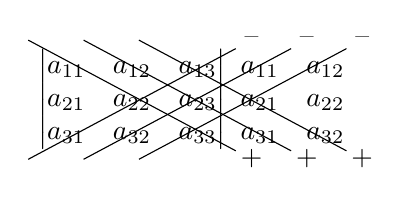
\begin{tikzpicture}
\node (A) {$\begin{vmatrix}
a_{11} & a_{12} & a_{13} \\
a_{21} & a_{22} & a_{23} \\
a_{31} & a_{32} & a_{33}
\end{vmatrix}$};
\node[right of=A, node distance=5.8em] (B) {$\begin{matrix}
a_{11} & a_{12} \\
a_{21} & a_{22} \\
a_{31} & a_{32}
\end{matrix}$};
\draw (A.south west) -- ++(7.5em,4em) ++(.2,.1) node {--};
\draw (A.south west) ++(2em,0) --  ++(7.5em,4em) ++(.2,.1) node {--};
\draw (A.south west) ++(4em,0) --  ++(7.5em,4em) ++(.2,.1) node {--};
\draw (A.north west) -- ++(7.5em,-4em) ++(.2,-.1) node {+};
\draw (A.north west) ++(2em,0) --  ++(7.5em,-4em) ++(.2,-.1) node {+};
\draw (A.north west) ++(4em,0) --  ++(7.5em,-4em) ++(.2,-.1) node {+};
\end{tikzpicture} \]
\end{corollary}
\begin{corollary} \label{determinantBound}
Let $A\in \F^{n\times n}$. Then $|\det(A)| \leq n! \norm{A}^n$.
\end{corollary}
\begin{proof}
We calculate using the Liebniz formula, \ref{matrixElementsBoundedByNorm} and the fact that $\#(S^n) = n!$ (TODO ref),
\begin{align*}
|\det(A)| &= \Big|\sum_{\sigma\in S^n}\sgn(\sigma)\prod_{i=1}^n[A]_{i,\sigma(i)}\Big| \\
&\leq \sum_{\sigma\in S^n}\Big|\prod_{i=1}^n[A]_{i,\sigma(i)}\Big| \\
&= \sum_{\sigma\in S^n}\prod_{i=1}^n\big|[A]_{i,\sigma(i)}\big| \\
&\leq \sum_{\sigma\in S^n}\prod_{i=1}^n\norm{A} \\
&= \sum_{\sigma\in S^n}\norm{A}^n \\
&= n!\norm{A}^n.
\end{align*}
\end{proof}
\begin{corollary}
The determinant function $\det: \F^{n\times n}\to \F$ is continuous.
\end{corollary}

\begin{proposition} \label{expansionDeterminantAroundIdentity}
Let $A\in \F^{n\times n}$ and $\lambda \in \F$. Then
\[ \det(\mathbb{1}_n + \lambda A) = 1 + \lambda \Tr(A) + \lambda^2P(\lambda), \]
where $P(\lambda)$ is a polynomial in $\lambda$ such that $|P(0)|\leq n(n-1)\norm{A}^2$ and $|P(1)| \leq 1 + n\norm{A} + n!\big(1 + \norm{A}\big)^n$.
\end{proposition}
\begin{proof}
We expand $\det(\mathbb{1}_n + \lambda A)$ using the Liebniz formula \ref{LiebnizFormula}:
\begin{align*}
\det(\mathbb{1}_n + \lambda A) &= \sum_{\sigma\in S^n}\sgn(\sigma)\prod_{i=1}^n[\mathbb{1}_n + \lambda A]_{i,\sigma(i)} \\
&= \sum_{\sigma\in S^n}\sgn(\sigma)\prod_{i=1}^n\big(\delta_{i,\sigma(i)} + \lambda [A]_{i,\sigma(i)}\big) \\
&= \prod_{i=1}^n\big(\delta_{i,i} + \lambda [A]_{i,i}\big) + \sum_{\sigma\in S^n\setminus\{\id\}}\sgn(\sigma)\prod_{i=1}^n\big(\delta_{i,\sigma(i)} + \lambda [A]_{i,\sigma(i)}\big).
\end{align*}
Now we expand the first part using \ref{productOfSum}:
\begin{align*}
\prod_{i=1}^n\big(\delta_{i,i} + \lambda [A]_{i,i}\big) &= \prod_{i=1}^n\big(1 + \lambda [A]_{i,i}\big)\\
&= \sum_{\seq{s_i}\in \{0,1\}^n}\prod_{i=0}^{n-1}\bigg(k\mapsto \begin{cases}
1 & (k=0) \\ \lambda[A]_{i,i} & (k=1)
\end{cases}\bigg)(s_i) \\
&= 1 + \lambda \sum_{i=0}^{n-1}[A]_{i,i} + \sum_{\seq{s_i}\in C}\prod_{i=0}^{n-1}\bigg(k\mapsto \begin{cases}
1 & (k=0) \\ \lambda [A]_{i,i} & (k=1)
\end{cases}\bigg)(s_i) \\
&= 1 + \lambda \Tr(A) + Q(\lambda),
\end{align*}
where $C$ is the subset of $\{0,1\}^n$ of strings that contains at least two ones and $Q(\lambda) \defeq \sum_{\seq{s_i}\in C}\prod_{i=0}^{n-1}\Big(k\mapsto \begin{cases}
1 & (k=0) \\ \lambda[A]_{i,i} & (k=1)
\end{cases}\Big)(s_i)$. Thus, by construction, every term of $Q(\lambda)$ is divisible by $\lambda^2$, so $Q(\lambda) = \lambda^2P'(\lambda)$ for some polynomial $P'(\lambda)$.

Now returning to $\sum_{\sigma\in S^n\setminus\{\id\}}\sgn(\sigma)\prod_{i=1}^n\big(\delta_{i,\sigma(i)} + \lambda [A]_{i,\sigma(i)}\big)$, note for every $\sigma\in S^n\setminus\{\id\}$ there must exist at least two distinct $i,j\in \interval[co]{0,n}$ such that $i\neq \sigma(i)$ and $j\neq \sigma(j)$ (TODO ref). The corresponding factors in $\prod_{i=1}^n\big(\delta_{i,\sigma(i)} + \lambda [A]_{i,\sigma(i)}\big)$ are divisible by $\lambda$, so the sum is a polynomial divisible by $\lambda^2$. We write $\lambda^2P^{\prime\prime}(\lambda) = \sum_{\sigma\in S^n\setminus\{\id\}}\sgn(\sigma)\prod_{i=1}^n\big(\delta_{i,\sigma(i)} + \lambda [A]_{i,\sigma(i)}\big)$. Now we define $P(\lambda) \defeq P'(\lambda) + P^{\prime\prime}(\lambda)$.

Finally, we compute the bounds of $P(0)$ and $P(1)$. For $P(0)$, if $\sigma\in S^n$ changes the place of more than two elements, then $\prod_{i=1}^n\big(\delta_{i,\sigma(i)} + \lambda [A]_{i,\sigma(i)}\big)$ contains at least three factors of $\lambda$. Even dividing out two, the contribution to $P^{\prime\prime}(0)$ is zero. If it changes the place of only two elements $i,j$ (i.e.\ it is a transposition), then it is equal to $\big|[A]_{i,j}[A]_{j,i}\big| \leq \norm{A}^2$ by \ref{matrixElementsBoundedByNorm}. Since there are $\frac{n(n-1)}{2}$ transpositions, there are $\frac{n(n-1)}{2}$ such terms. By a similar reasoning, we bound $\prod_{i=0}^{n-1}\Big(k\mapsto \begin{cases}
1 & (k=0) \\ \lambda[A]_{i,i} & (k=1)
\end{cases}\Big)(s_i)$ by $\big|[A]_{i,i}[A]_{j,j}\big|$ if $s$ has ones only at locations $i,j$. Otherwise the corresponding term is zero. Thus for $P'(0)$ we also get a bound of $\frac{n(n-1)}{2}\norm{A}^2$. Adding these together gives $n(n-1)\norm{A}^2$.

For $P(1)$, we have $P(1) = \det(\mathbb{1}_n + A) - 1 - \Tr(A)$, so using \ref{matrixElementsBoundedByNorm} and \ref{determinantBound}, we have
\begin{align*}
\big|P(1)\big| &\leq 1 + \big|\Tr(A)\big| + \big|\det(\mathbb{1}_n + A)\big| \\
&\leq 1 + n\norm{A} + n!\norm{\mathbb{1}_n + A}^n \\
&\leq 1 + n\norm{A} + n!\big(1 + \norm{A}\big)^n.
\end{align*}
\end{proof}

\subsubsection{Laplace expansion}
\begin{definition}
Let $A\in\F^{n\times n}$ be a square matrix. A \udef{minor determinant} or \udef{minor} is the determinant of a submatrix. In particular the \udef{$(i,j)$-minor} $M_{i,j}$ is the minor
\[ M_{i,j} \defeq \det([A]_{(1:n)\setminus\{i\},(1:n)\setminus\{j\}}). \]

The \udef{$(i,j)$-cofactor} $C_{i,j}$ is defined as
\[ C_{i,j} \defeq (-1)^{i+j}M_{i,j}. \]
\end{definition}
\begin{proposition}[Laplace expansion] \label{LaplaceExpansion}
Let $A\in\F^{n\times n}$. Then
\[ \det(A) = \sum_{i=1}^n [A]_{i,j}C_{i,j} = \sum_{i=1}^n [A]_{j,i}C_{j,i} \]
for all $j\in 1:n$.
\end{proposition}
This is also known as ``expansion along the $j^\text{th}$ column'', resp., row.
\begin{proof}
Fix some $j\in 1:n$. Then we can calculate
\begin{align*}
\det(A) &=  \sum_{\sigma\in S^n}\sgn(\sigma)\prod_{k=1}^n[A]_{k,\sigma(k)} = \sum_{i=1}^n\sum_{\substack{\sigma\in S^n \\ \sigma(i)=j}}\sgn(\sigma)\prod_{k=1}^n[A]_{k,\sigma(k)} \\
&= \sum_{i=1}^n [A]_{i,j}\sum_{\substack{\sigma\in S^n \\ \sigma(i)=j}}\sgn(\sigma)\prod_{k\in (1:n)\setminus\{j\}}^n[A]_{k,\sigma(k)} = \sum_{i=1}^n [A]_{i,j}C_{i,j}.
\end{align*}
The expression for column expansion can be obtained by transposition.
\end{proof}

\subsubsection{Volume}

\subsubsection{Properties}
\begin{lemma}
Let $A\in\F^{n\times n}$. Then
\[ \det(A^\transp) = \det(A). \]
\end{lemma}
\begin{proof}
We calculate using the Leibniz formula:
\begin{align*}
\det(A^\transp) &= \sum_{\sigma\in S^n}\sgn(\sigma)\prod_{i=1}^n[A^\transp]_{i,\sigma(i)} = \sum_{\sigma\in S^n}\sgn(\sigma)\prod_{i=1}^n[A]_{\sigma(i),i} \\
&= \sum_{\sigma\in S^n}\sgn(\sigma)\prod_{i=1}^n[A]_{i,\sigma^{-1}(i)} = \sum_{\sigma\in S^n}\sgn(\sigma^{-1})\prod_{i=1}^n[A]_{i,\sigma^{-1}(i)} = \det(A).
\end{align*}
\end{proof}

\begin{lemma}
Let $A\in\F^{n\times n}$. Then
\begin{enumerate}
\item $\det(\lambda A) = \lambda^n\det(A)$;
\item $\det(\overline{A}) = \overline{\det(A)}$;
\item $\det(A^*) = \overline{\det(A)}$;
\item if $A$ is triangular, then
\[ \det(A) = \prod_{i=1}^n [A]_{i,i}. \]
\end{enumerate}
\end{lemma}

\begin{proposition}
Let $A,B\in\F^{n\times n}$. Then
\[ \det(AB) = \det(A)\det(B). \]
\end{proposition}
\begin{proof}
First assume $\det(B) = 0$. Then $AB$ is not invertible, for if $AB$ were invertible, $B$ would have inverse $(AB)^{-1}A$. So $\det(AB) = 0$ and the formula holds.

Now assume $\det(B) \neq 0$, then $A\mapsto \det(AB)/\det(B)$ satisfies the definition of a determinant map and thus is equal to $\det$.
\end{proof}
\begin{corollary}
If $U$ is unitary, then $|\det(U)| = 1$.
\end{corollary}
\begin{proof}
$1=\det{\mathbb{1}} = \det(U^*U) = \det(U^*)\det(U) = \overline{\det(U)}\det(U) = |\det(U)|$.
\end{proof}
\begin{corollary}
Let $A,B\in\F^{n\times n}$. Then
\[ \det(AB) = \det(BA). \]
In fact we can arbitrarily commute any matrix product inside the determinant.
\end{corollary}
\begin{corollary}
The determinant of a matrix of a linear map is independent of the choice of basis:
\[ \det(L)_{\beta}^{\beta} = \det(L)_{\beta'}^{\beta'}. \]
\end{corollary}
This allows us to make the following definition:
\begin{definition}
The \udef{determinant} of a linear map on a finite-dimensional vector space is the determinant of any matrix representation of that map.
\end{definition}

\begin{lemma}
Let $A\in\F^{m\times m}$ and $n\in\N$. Then
\[ \det\begin{bmatrix}
\mathbb{1}_n & \mathbb{0} \\ \mathbb{0} & A
\end{bmatrix} = \det(A) = \det\begin{bmatrix}
A & \mathbb{0} \\ \mathbb{0} & \mathbb{1}_n
\end{bmatrix}. \]
\end{lemma}
\begin{proof}
By induction on $n$.
\end{proof}

\begin{lemma}
Let $A,B,C$ be conformal matrices and $A,D$ square. Then
\[ \det\begin{bmatrix}A & B \\ \mathbb{0} & D \end{bmatrix} = \det(A)\det(D). \]
\end{lemma}
\begin{proof}
This follows from
\[ \begin{bmatrix}A & B \\ \mathbb{0} & D \end{bmatrix} = \begin{bmatrix}\mathbb{1} & \mathbb{0} \\ \mathbb{0} & D \end{bmatrix} \begin{bmatrix}\mathbb{1} & B \\ \mathbb{0} & \mathbb{1} \end{bmatrix} \begin{bmatrix}A & \mathbb{0} \\ \mathbb{0} & \mathbb{1} \end{bmatrix}, \]
the product rule, the previous lemma and the fact that the central matrix is triangular with only ones on the diagonal.
\end{proof}

\begin{lemma} \label{blockDeterminant}
Let $M = \begin{pmatrix}
A & B \\ C & D
\end{pmatrix}$ be a partitioned matrix. Then
\begin{align*}
\det(M) &= \det(A)\det(D-CA^{-1}B) \\
&= \det(D)\det(A-BD^{-1}C)
\end{align*}
if $A$, resp. $D$, is invertible.
\end{lemma}
\begin{proof}
This follows straight from the Schur complement.
\end{proof}
\begin{corollary}[Cauchy expansion of the determinant]
Let $A\in\F^{n\times n}, \vec{x},\vec{y}\in\F^n$ and $c\in \F$. Then
\[ \det \begin{bmatrix}
c & \vec{x}^\transp \\ \vec{y} & A
\end{bmatrix} = (c-\vec{x}^\transp A^{-1}\vec{y})\det(A) = c\det(A) - \vec{x}^\transp \adj(A) \vec{y}. \]
\end{corollary}
\begin{corollary}
Let $A,B,C,D\in\F^{n\times n}$.
\begin{enumerate}
\item If $A$ or $D$ is invertible and commutes with $B$, then
\[ \det\begin{bmatrix}
A & B \\ C & D
\end{bmatrix} = \det(DA-CB). \]
\item If $A$ or $D$ is invertible and commutes with $C$, then
\[ \det\begin{bmatrix}
A & B \\ C & D
\end{bmatrix} = \det(AD-BC). \]
\end{enumerate}
\end{corollary}

\begin{lemma}
Let $a,b\in\R$. Then
\[ \det(a\mathbb{1}_n+b\mathbb{J}_n) = a^{n-1}(a+nb). \]
\end{lemma}
\begin{proof}
We can partition $a\mathbb{1}_n+b\mathbb{J}_n$ and use the ERO $R_i\to R_i-R_1$ for $1<i\leq n$ to obtain:
\[ a\mathbb{1}_n+b\mathbb{J}_n = \begin{pmatrix}
a+b & b\mathbb{J}^{1\times (n-1)} \\
b\mathbb{J}^{(n-1)\times 1} & a\mathbb{1}_{n-1}+b\mathbb{J}_{n-1}
\end{pmatrix} = \begin{pmatrix}
a+b & b\mathbb{J}^{1\times (n-1)} \\
-a\mathbb{J}^{(n-1)\times 1} & a\mathbb{1}_{n-1}
\end{pmatrix}. \]
Then by \ref{blockDeterminant}, we have
\[ \det(a\mathbb{1}_n+b\mathbb{J}_n) = a^{n-1}(a+b +b\mathbb{J}^{1\times (n-1)}\mathbb{J}^{(n-1)\times 1}) = a^{n-1}(a+nb). \]
\end{proof}

\begin{lemma}[Weinstein-Aronszajn identity]
Let $A\in\F^{m\times n}$ and $B\in\F^{n\times m}$. Then
\[ \det(\mathbb{1}_{m} + AB) = \det(\mathbb{1}_{n} + BA). \]
Also, for any $\lambda\in\R_0$,
\[ \det(AB - \lambda\mathbb{1}_{m}) = (-\lambda)^{m-n}\det(BA - \lambda\mathbb{1}_{n}). \]
\end{lemma}
This is also sometimes referred to as the Sylvester determinant identity.
\begin{proof}
Applying the two equalities in \ref{blockDeterminant} to the matrix
\[ M = \begin{bmatrix}
\mathbb{1}_m & -A \\
B & \mathbb{1}_n
\end{bmatrix} \]
give
\begin{align*}
M &= \det(\mathbb{1}_m)\det(\mathbb{1}_n - B\mathbb{1}_m^{-1}(-A)) = \det(\mathbb{1}_n+BA) \\
&= \det(\mathbb{1}_n)\det(\mathbb{1}_m - (-A)\mathbb{1}_n^{-1}B) = \det(\mathbb{1}_m+AB).
\end{align*}
\end{proof}
\begin{corollary}[Matrix determinant lemma]
Let $A\in\F^{n\times n}$ and $\vec{u},\vec{v}\in\F^n$. Then
\begin{align*}
\det(A+\vec{u}\vec{v}^\transp) &= \det(A)\det(\mathbb{1}_n + A^{-1}\vec{u}\vec{v}^\transp) \\
&= \det(A)(\mathbb{1}_n + \vec{v}^\transp A^{-1}\vec{u}) \\
&= \det(A) + \vec{v}^\transp \adj(A)\vec{u},
\end{align*}
which is interesting because $\vec{v}^\transp A^{-1}\vec{u} \in\F$  and $\vec{v}^\transp \adj(A)\vec{u}\in\F$ are scalars.
\end{corollary}

TODO
\[ \log\det M=\Tr\log M \]


\subsection{Adjugate}
\begin{definition}
Let $A\in\F^{n\times n}$ be a square matrix. The \udef{adjugate matrix} or \udef{classical adjoint} $\adj(A)$ is the transposed cofactor matrix:
\[ [\adj(A)]_{ij} = C_{ji} \]
where $C_{ij}$ is the $(i,j)-$cofactor.
\end{definition}

\begin{lemma}
Let $A\in\F^{n\times n}$, $\vec{b}\in \F^n$ and $k\in(1:n)$. Then
\[ \det(\left[\begin{cases}
[A]_{ij} & (j\neq k) \\
[\vec{b}]_i & (j=k)
\end{cases}\right]) = [\adj(A)b]_k \]
\end{lemma}
\begin{proof}
We calculate
\[ [\adj(A)\vec{b}]_k = \sum_l [\adj(A)]_{kl}[\vec{b}]_l = \sum_l C_{lk}[\vec{b}]_l. \]
Now in the definition of $C_{lk}$, the $k^\text{th}$ column is excluded. So the $(l,k)-$cofactor of $A$ is the same as the $(l,k)-$cofactor of 
\[ \left[\begin{cases}
[A]_{ij} & (j\neq k) \\
[\vec{b}]_i & (j=k)
\end{cases}\right] \]
which is the matrix where the $k^\text{th}$ column of $A$ is replaced by $\vec{b}$. Then $\sum_l C_{lk}[\vec{b}]_l$ is the determinant of this matrix by \ref{LaplaceExpansion}.
\end{proof}

\begin{proposition} \label{adjunctDeterminant}
Let $A\in\F^{n\times n}$. Then
\[ A\cdot\adj(A) = \adj(A)\cdot A = \det(A) \mathbb{1}_n. \]
\end{proposition}
\begin{proof}
\[ [\adj(A)\cdot A]_{ij} = \sum_k [A]_{ik}C_{jk} \]
Clearly if $i=j$, we have the Laplace expansion \ref{LaplaceExpansion} and the expression equals $\det(A)$. If $i\neq j$, then the $j^\text{th}$ row does not enter into the expression (it is left out of the $(i,j)-$minor) and thus may just as well be replaced by a copy of the $i^\text{th}$ row. In this case we get the expression for the determinant of a matrix with two identical rows. This must be $0$.
\end{proof}
\begin{corollary} \label{inverseAdjunctDeterminant}
Let $A\in\F^{n\times n}$ be invertible. Then
\[ A^{-1} = \frac{1}{\det(A)}\adj(A). \]
\end{corollary}

\begin{proposition}
Let $A,B\in\F^{n\times n}$ be square matrices. Then
\begin{enumerate}
\item $\adj(\mathbb{0}_n) = \mathbb{0}_n$;
\item $\adj(\mathbb{1}_n) = \mathbb{1}_n$;
\item $\adj(\lambda A) = \lambda^{n-1}\adj(A)$ for any $\lambda\in \F$;
\item $\adj(A^\transp) = \adj(A)^\transp$;
\item $\det(\adj(A)) = \det(A)^{n-1}$;
\item $\adj(AB) = \adj(A)\adj(B)$.
\end{enumerate}
\end{proposition}
\begin{proof}
Points 2. and 5. are direct consequences of \ref{adjunctDeterminant}. TODO rest.
\end{proof}
Cauchy-Binet

\subsection{Generalised inverses or pseudoinverses}
\subsubsection{Moore-Penrose pseudoinverse}

\subsection{Pfaffian}

\subsection{Vectorisation}
For calculations it is often useful to put the matrix of coordinates into a column vector. The process of fitting a matrix into a column vector is known as the \udef{vectorisation} of a matrix. Two obvious ways to do this are by going row-by-row or column by column.
\begin{itemize}
\item Column-by-column we get
\[ \vectorisation_C: \R^{m\times n}\to \R^{mn\times 1}: A \mapsto \vectorisation_C(A) = [a_{1,1},\ldots,a_{m,1}, a_{1,2},\ldots, a_{m,2}, \;\; \ldots \;\; , a_{1,n}, \ldots, a_{m,n}]^\transp \]
\begin{example}
\[ \text{If} \qquad A = \begin{pmatrix}
a & b \\ c & d
\end{pmatrix}, \qquad \text{then} \qquad \vectorisation_C(A) = \begin{pmatrix}
a \\ c \\ b \\ d
\end{pmatrix}. \]
\end{example}
\item Row-by-row we get
\[ \vectorisation_R: \R^{m\times n}\to \R^{mn\times 1}: A \mapsto \vectorisation_R(A) = [a_{1,1},\ldots,a_{1,n}, a_{2,1},\ldots, a_{2,n}, \;\; \ldots \;\; , a_{m,1}, \ldots, a_{m,n}]^\transp \]
\begin{example}
\[ \text{If} \qquad A = \begin{pmatrix}
a & b \\ c & d
\end{pmatrix}, \qquad \text{then} \qquad \vectorisation_R(A) = \begin{pmatrix}
a \\ b \\ c \\ d
\end{pmatrix}. \]
\end{example}
\end{itemize}
Obviously these are related by
\[ \vectorisation_C(A) = \vectorisation_R(A^\transp) \]

Vectorisation is a self-adjunction in the monoidal closed structure of any category of matrices. (TODO)
\subsection{The Hadamard product}
\[ \vectorisation(A\circ B) = \vectorisation(A) \circ \vectorisation(B) \]
This works for both $\vectorisation_C$ and $\vectorisation_R$.
\subsection{The outer product}
Given two column vectors $\vec{u} = [u_1 \hdots u_m]^\transp$ and $\vec{v} = [v_1 \hdots v_n]^\transp$, the \udef{outer product} is defined by
\[ \vec{u}\otimes \vec{v} = \vec{u}\vec{v}^\transp = \begin{bmatrix}
u_1 \\ \vdots \\ u_m
\end{bmatrix} \begin{bmatrix}
v_1 & \hdots & v_n
\end{bmatrix} = \begin{bmatrix}
u_1v_1 & \hdots & u_1v_n \\
\vdots & \ddots & \vdots \\
u_mv_1 & \hdots & u_m v_n
\end{bmatrix} \]
\subsection{The Kronecker product}
Given two matrices $A,B$ of dimensions $m\times n$ and $p\times q$, the \udef{Kronecker product} yields a $(pm\times qn)$-matrix:
\[ A\otimes B = \begin{bmatrix}
a_{1,1}B & \hdots & a_{1,n}B \\
\vdots & \ddots & \vdots \\
a_{m,1}B & \hdots & a_{m,n}B
\end{bmatrix} \]

The same symbol is used as for the outer product, because the Kronecker product can be seen as a generalisation of the outer product. Indeed for column vectors $\vec{u}, \vec{v}$ we have the identities
\begin{align}
\vec{u}\otimes_{\text{Kron}} \vec{v} &= \vectorisation_R(\vec{u}\otimes_\text{outer} \vec{v}) \\
&= \vectorisation_C(\vec{v}\otimes_\text{outer} \vec{u})
\end{align}
and \[ \vec{u}\otimes_\text{outer}\vec{v} = \vec{u}\otimes_{\text{Kron}} \vec{v}^\transp \]

In terms of matrix elements we can write, assuming the indices start at zero
\[ (A\otimes B)_{i,j} = a_{\lfloor{i/p}\rfloor, \lfloor{j/q}\rfloor}b_{i\%p,j\%q}. \]
where $\%$ denotes the remainder. For indices starting from 1, we have
\[ (A\otimes B)_{i,j} = a_{\lceil{i/p}\rceil, \lceil{j/q}\rceil}b_{(i-1)\%p+1,(j-1)\%q+1}. \]

\subsubsection{Properties}
The Kronecker product is bilinear and associative.
\begin{itemize}
\item[\textbf{Transpose}]
\[ (A\otimes B)^\transp = A^\transp \otimes B^\transp \]
\item[\textbf{Determinant}]
\[ \det(A\otimes B) = \det(A)^m\det(B)^n \]
if $A$ is an $n\times n$ matrix and $B$ an $m\times m$ matrix.
\item[\textbf{Trace}]
\[ \Tr(A\otimes B) = \Tr(A)\Tr(B) \]
\item[\textbf{Mixed product}]
Let $A,B,C,D$ be conformal matrices, then
\[ (A\otimes B)(C \otimes D) = (AC)\otimes (BD). \]
The proof is as follows:
\begin{align}
(A\otimes B)(C \otimes D) &= \begin{bmatrix}
a_{1,1}B & \hdots & a_{1,n}B \\
\vdots & \ddots & \vdots \\
a_{m,1}B & \hdots & a_{m,n}B
\end{bmatrix}\begin{bmatrix}
c_{1,1}D & \hdots & c_{1,n}D \\
\vdots & \ddots & \vdots \\
c_{m,1}D & \hdots & c_{m,n}D
\end{bmatrix} \\
&= \begin{bmatrix}
\sum_k a_{1,k}c_{k,1} BD & \hdots & \sum_k a_{1,k}c_{k,p} BD \\
\vdots & \ddots & \vdots \\
\sum_k a_{m,k}c_{k,1} BD & \hdots & \sum_k a_{m,k}c_{k,p} BD
\end{bmatrix}  =  \begin{bmatrix}
(AC)_{1,1} BD & \hdots & (AC)_{1,p} BD \\
\vdots & \ddots & \vdots \\
(AC)_{m,1} BD & \hdots & (AC)_{m,p} BD
\end{bmatrix}\\
&= (AC)\otimes (BD)
\end{align}
Using the fact that multiplication of two block matrices can be carried out as if their blocks were scalars.

As an immediate consequence:
\[ A\otimes B = (I_n\otimes B)(A\otimes I_k) = (A\otimes I_k)(I_n \otimes B). \]

\item[\textbf{Inverse}]
The product $A\otimes B$ is invertible iff $A$ and $B$ are invertible. In that case the inverse is given by
\[ (A\otimes B)^{-1} = A^{-1}\otimes B^{-1}. \]
This follows easily from the mixed product.
\item[\textbf{Moore-Penrose pseudoinverse}]
\[ (A\otimes B)^+ = A^+\otimes B^+. \]

\item[\textbf{A vectorisation trick}]
Let $A,B,C$ be matrices of dimensions $k\times l, l\times m$ and $m\times n$. Then
\[ \vectorisation(ABC) = (C^\transp\otimes A)\vectorisation(B). \]
From this we obtain some other formulations:
\begin{align}
\vectorisation(ABC) &= (I_n\otimes AB)\vectorisation(C) \\
&= (C^\transp B^\transp \otimes I_k)\vectorisation(A) \\
\vectorisation(AB) &= (I_m\otimes A)\vectorisation(B) = (B^\transp \otimes I_k)\vectorisation(A)
\end{align}
\end{itemize}

\subsection{The commutator}
\begin{theorem}[Shoda's theorem]
Let $A\in\F^{n\times n}$. Then there exists $X,Y$ such that $A=[X,Y] = XY-YX$ \textup{if and only if} $\Tr(A) = 0$.
\end{theorem}
\begin{proof}
Assume $A = [X,Y]$. Then $\Tr(A) = \Tr(XY) -\Tr(YX) = \Tr(XY) - \Tr(XY) = 0$.

Conversely, assume $\Tr(A) = 0$. By \ref{averageTraceOverDiagonal} $A$ is similar to a matrix $B$ that has zeros on the diagonal. Let $X = \diag(1,2,\ldots, n)$ and
\[ [Y]_{i,j} = \begin{cases}
(i-j)^{-1}[B]_{i,j} & (i\neq j) \\
1 & (i=j).
\end{cases} \]
Then
\[ [X,Y]_{i,j} = [XY-YX]_{i,j} = i[Y]_{i,j}-j[Y]_{i,j} = (i-j)[Y]_{i,j} = [B]_{i,j}. \]
So $B$ is the commutator $[X,Y]$. Then $A$ is the commutator $[SXS^{-1}, SYS^{-1}]$.
\end{proof}

\subsection{Kruskal rank and spark}
\begin{definition}
Let $A\in \F^{m\times n}$. The \udef{Kruskal rank} is the largest number $\KruskalRank(A)$ such that all $\KruskalRank(A)$-sets of columns are linearly independent.
\end{definition}
\begin{lemma}
Let $A\in \F^{m\times n}$. Then $\KruskalRank(A) \leq \Rank(A)$.
\end{lemma}
\begin{proof}
If $\Rank(A) = k$, then there exists a $k$-set of columns that spans $\Col(A)$. Then every linearly independent set is smaller than $k$ by the Steinitz exchange lemma \ref{SteinitzExchange} and $\KruskalRank(A) \leq k$.
\end{proof}

\begin{definition}
Let $A\in \F^{m\times n}$. Then the \udef{spark} of $A$ is defined as
\[ \operatorname{spark}(A) \defeq \min\setbuilder{\norm{x}_0}{x\in\Null(A)} \]
where $\norm{x}_0$ is the number of non-zero elements of $x$.
\end{definition}
TODO $\norm{\cdot}_0$ norm for finite fields.

\begin{lemma}
Let $A\in \F^{m\times n}$. Then
\[ \operatorname{spark}(A) = \KruskalRank(A) + 1. \]
\end{lemma}
\begin{proof}
TODO
\end{proof}

\begin{lemma}
Let $A\in \F^{m\times n}$. If $\Rank(A) = n$, then $\KruskalRank(A) = n$.
\end{lemma}

\begin{proposition}
Let $A\in \F^{m\times n}$. Then
\[ \KruskalRank(A) \geq \frac{1}{\mu(A)} \]
where $\mu(A) = \max_{i\neq j} \frac{|\inner{[A]_{_,i},[A]_{-,j}}|}{\norm{[A]_{_,i}}\norm{[A]_{_,j}}}$.
\end{proposition}
\begin{proof}
TODO
\end{proof}


\section{Eigenvalues and eigenvectors}
\subsection{The spectrum}
In this section we study vectors that are mapped to multiples of themselves by a given matrix $A$, i.e.\ vectors $\vec{v}$ such that
\[ A\vec{v} = \lambda \vec{v} \qquad\text{for some $\lambda\in\F$.} \]
Clearly for this to be possible, $A$ needs to be square.
\begin{definition}
Suppose $A\in \F^{n\times n}$.
\begin{itemize}
\item  A scalar $\lambda\in \mathbb{F}$ is called an \udef{eigenvalue} of $A$ if there exists a $\vec{v}\in \F^n$ such that $\vec{v}\neq 0$ and $A\vec{v} = \lambda v$.
\item Such a vector $\vec{v}$ is called an \udef{eigenvector}.
\item The set of all eigenvectors associated with an eigenvalue $\lambda$ is called the \udef{eigenspace} $E_\lambda(A)$. Because
\[ E_\lambda(A) = \ker(\ell_{\lambda \mathbb{1}_{n} - A}), \]
it is indeed a vector space.

The dimension of $E_\lambda(A)$ is the \udef{geometric multiplicity} of $\lambda$.
\end{itemize}
The set of all eigenvalues is called the \udef{spectrum} of $A$.
\end{definition}
\begin{proposition}
Let $A\in \F^{n\times n}$ and $\lambda\in \mathbb{F}$, then
\[ \text{$\lambda$ is an eigenvalue of $A$} \qquad \iff \qquad \text{$\lambda \mathbb{1}_{n} - A$ is invertible.} \]
\end{proposition}
\begin{proof}
The equation $A\vec{v} = \lambda \vec{v}$ is equivalent to $(A-\lambda \mathbb{1}_n)\vec{v} = 0$. So there exist eigenvectors associated to $\lambda$ iff the kernel of $\ell_{A-\lambda \mathbb{1}_n}$ is not trivial iff $\ell_{A-\lambda \mathbb{1}_n}$ is injective (\ref{injectivityKernelTriviality}) iff $\ell_{A-\lambda \mathbb{1}_n}$ is invertible (\ref{invertibleFiniteDim}) iff $A-\lambda \mathbb{1}_n$ is invertible (\ref{invertibleMapInvertibleMatrix}).
\end{proof}

\begin{proposition}[Gerschgorin circle theorem]
Let $A\in \F^{n\times n}$. If $\lambda$ is an eigenvalue of $A$, then there is an $i\in 1:n$ such that
\[ |\lambda - [A]_{ii}| \leq \sum_{\substack{j\in 1:n \\ j \neq i}}|[A]_{ij}|. \]
\end{proposition}
\begin{proof}
If $|\lambda - [A]_{ii}| > \sum_{\substack{j\in 1:n \\ j \neq i}}|[A]_{ij}|$ for all $i$, then $(A-\lambda\mathbb{1})$ is strictly diagonally dominant and thus invertible by \ref{invertibleDiagonallyDominant}.
\end{proof}

\begin{proposition}
Let $A\in\F^{n\times n}$ be a matrix. Suppose $\lambda_1, \ldots, \lambda_m$ are distinct eigenvalues of $A$ and $\vec{v}_1,\ldots, \vec{v}_m$ are corresponding eigenvectors. Then $\{\vec{v}_1,\ldots, \vec{v}_m\}$ is linearly independent.
\end{proposition}
\begin{proof}
The proof goes by contradiction. Assume $\{\vec{v}_1,\ldots, \vec{v}_m\}$ is linearly dependent. Let $k$ be the smallest positive integer such that
\[ \vec{v}_k \in \Span\{\vec{v}_1,\ldots, \vec{v}_{k-1}\}. \]
So there exists a nontrivial linear combination
\[ \vec{v}_k = a_1\vec{v}_1+\ldots +a_{k-1}\vec{v}_{k-1}. \]
Multiplying by $A$ gives
\[ \lambda_k\vec{v}_k = a_1\lambda_k\vec{v}_1+\ldots +a_{k-1}\lambda_k\vec{v}_{k-1}. \]
Multiplying the previous combination by $\lambda_k$ and subtracting both equations gives
\[ 0= a_1(\lambda_k-\lambda_1)\vec{v}_1 +\ldots + a_{k-1}(\lambda_k - \lambda_{k-1})\vec{v}_{k-1}. \]
By assumption of linear independence of $\{\vec{v}_1,\ldots, \vec{v}_{k-1}\}$ this combination must be trivial, however none of the $(\lambda_k-\lambda_i)$ can be zero, so all the $a_i$ must be zero. This is a contradiction with the assumption of linear dependence.
\end{proof}
\begin{corollary}
The matrix $A\in\F^{n\times n}$ has at most $n$ linearly independent eigenvalues.
\end{corollary}
\begin{corollary}
Suppose $\lambda_1, \ldots, \lambda_m$ are distinct eigenvalues of $A$. Then
\[ E_{\lambda_1}(A) \oplus \ldots \oplus E_{\lambda_m}(A) \]
is a direct sum. Furthermore, the sum of geometric multiplicities is less than or equal to the dimension of $V$:
\[ \dim E_{\lambda_1}(A) + \ldots + \dim E_{\lambda_m}(A) \leq \dim V. \]
\end{corollary}

\subsubsection{The characteristic equation}
\begin{definition}
Let $A\in\F^{n\times n}$. The \udef{characteristic polynomial} $p_A(x)$ of $A$. Is the polynomial
\[ p_A(x) \defeq \det(x\mathbb{1}_n - A). \]
\end{definition}
The characteristic polynomial is also sometimes defined as $\det(A - x\mathbb{1}_n)$. This differs by a sign $(-1)^{n}$.
\begin{lemma}
The characteristic polynomial of any square matrix is a monic polynomial.
\end{lemma}
\begin{lemma}
The characteristic polynomials of similar matrices are identical.
\end{lemma}

\begin{proposition}
Let $A\in\F^{n\times n}$. Then $p_A(x)$ can be factorised as
\[ p_A(x) = \prod_{i=1}^m (x - \lambda_i)^{m_i}  \]
where $\lambda_i$ are the eigenvalues of $A$ and the multiplicities $m_i$ are positive integers such that $\sum_{i=1}^m m_i = n$.
\end{proposition}
\begin{corollary}
The eigenvalues of $A$ are the solutions of the equation
\[ p_A(x) = 0. \]
\end{corollary}
\begin{corollary}
The determinant of a matrix is the product of its eigenvalues, counting algebraic multiplicity: for $A\in\F^{n\times n}$
\[ \det(A) = \prod_{i=1}^m\lambda_i^{m_i}. \]
\end{corollary}
\begin{proof}
We have
\[ \det(A) = (-1)^n\det(0-A) = (-1)^np_A(0) = (-1)^n\prod_{i=1}^m(0 - \lambda_i)^{m_i} = \prod_{i=1}^m\lambda_i^{m_i}. \]
\end{proof}

\begin{definition}
Let $A\in\F^{n\times n}$. The equation
\[ p_A(x) = \det(x\mathbb{1}_n - A) = 0 \]
is called the \udef{characteristic equation} of $A$.

Let $\lambda$ be a solution of the characteristic equation. The multiplicity of $\lambda$ as a root of $p_A(x)$ is the \udef{algebraic multiplicity} of $\lambda$.
\end{definition}
\begin{lemma}
Let $A\in\F^{n\times n}$ and $\lambda$ be an eigenvalue of $A$.

The geometric multiplicity of $\lambda$ is less than or equal to the algebraic multiplicity of $\lambda$.
\end{lemma}
\begin{proof}
Set $k=\dim E_\lambda$. Take a basis of $E_\lambda(A)$ and extend it to a basis $\beta$ of $\F^{n}$. With respect to this basis the matrix of $\ell_A$ is of the form
\[ (\ell_A)_\beta^\beta =  \begin{pmatrix}
\lambda \mathbb{1}_k & B \\ 0 & C
\end{pmatrix} = P^{-1}(\ell_A)_\mathcal{E}^\mathcal{E}P = P^{-1}AP \]
for some matrices $B,C$ and some invertible matrix $P$ where $\mathcal{E}$ is the standard basis of $\F^n$. Then 
\[ p_A(x)= p_{P^{-1}AP} = p_{\lambda \mathbb{1}_{k}}(x)p_C(x) = (\lambda - x)^kp_C(x), \]
so the algebraic multiplicity of $\lambda$ is at least the geometric multiplicity $k$. It may be greater if $\lambda$ is also an eigenvector of $C$, but in this case the eigenvector is a linear combination of the eigenvectors already chosen for $\beta$.
\end{proof}

\subsubsection{Diagonalisable matrices}
\begin{definition}
A matrix $A\in\F^{n\times n}$ is called \udef{diagonalisable} if $\F^n$ has a basis of eigenvectors of $A$.
\end{definition}
\begin{proposition}
Let $A\in\F^{n\times n}$ and let $\lambda_1,\ldots, \lambda_m$ denote the distinct eigenvalues of $A$. The following are equivalent:
\begin{enumerate}
\item $A$ is diagonalisable;
\item there exist $1$-dimensional subspaces $U_1,\ldots, U_n$ of $A$, each invariant under $\ell_A$, such that
\[ \F^n = U_1\oplus \ldots \oplus U_n; \]
\item $\F^n = E_{\lambda_1}(A) \oplus \ldots \oplus E_{\lambda_m}(A);$
\item $n = \dim E_{\lambda_1}(A) + \ldots + \dim E_{\lambda_m}(A);$
\item for each $\lambda_i$ the geometric multiplicity is equal to the algebraic multiplicity and the sum of algebraic multiplicities is $n$.
\end{enumerate}
\end{proposition}
In the case of complex vector spaces, the sum of algebraic multiplicities is always $n$ by the fundamental theorem of algebra.
\begin{corollary}
If $A\in\F^{n\times n}$ has $n$ distinct eigenvalues, then $A$ is diagonalisable.
\end{corollary}
So a matrix may fail to be diagonalisible for two reasons: not enough geometric multiplicity or not enough geometric and algebraic multiplicity

\subsection{Spectral theorem}
\begin{theorem}
Let $V$ be a complex finite-dimensional inner product space. Let $L$ be an operator on $V$. Then
\begin{enumerate}
\item there exists an orthonormal basis of $V$ consisting of eigenvectors of $L$ \textup{if and only if} $L$ is normal;
\item if $L$ is self-adjoint, then the eigenvalues of $L$ are real.
\end{enumerate}
\end{theorem}

TODO: replace following: + in real case we need self-adjoint!
\begin{theorem}[Spectral theorem for matrices]
Let $V$ be a finite-dimensional inner product space over $\R$ or $\C$. Let $L=L^*$ be self-adjoint. Then
\begin{enumerate}
\item there exists an orthonormal basis of $V$ consisting of eigenvectors of $L$;
\item the eigenvalues of $L$ are real.
\end{enumerate}
\end{theorem}
\begin{proof}
We first prove the theorem for complex vector spaces. The proof is by finite induction:

By the fundamental theorem of algebra the characteristic polynomial has at least 1 root $\lambda_1$. Choose a corresponding eigenvector $\vec{v}_1$. Then by
\[ \lambda_1\inner{\vec{v}_1,\vec{v}_1} = \inner{\vec{v}_1, L\vec{v}_1} = \inner{L\vec{v}_1, \vec{v}_1} = \overline{\lambda_1}\inner{\vec{v}_1, \vec{v}_1}, \]
$\lambda_1$ is real.

Now $\Span\{\vec{v}_1\}^\perp$ is invariant under $L$:
\[ \vec{x}\in \Span\{\vec{v}_1\}^\perp \quad\iff\quad \inner{\vec{x},\vec{v}_1} = 0 \quad\implies\quad \inner{L\vec{x},\vec{v}_1} = \inner{\vec{x},L\vec{v}_1} = \lambda_1\inner{\vec{x},\vec{v}_1} = 0. \]

We can now apply the same argument to $L|_{\Span\{\vec{v}_1\}^\perp}:\Span\{\vec{v}_1\}^\perp\to \Span\{\vec{v}_1\}^\perp$, whose eigenvector are orthogonal to $v_1$. Finite induction then finishes the proof in the complex case. 

In the real case: we can linearly extend $L$ to be an operator $L_\C$ on the complexification $V_\C$. Then $L_\C$ has formally the same characteristic polynomial as $L$, except now interpreted as a function $\C\to\C$, not $\R\to\R$. Now we know the roots of $p_{L_\C}(x)$ are real, so they are also roots of $p_L(x)$. The rest of the proof can be completed in the same way. 
\end{proof}

The spectral decomposition is a special case of both the Schur decomposition and the singular value decomposition.

TODO: Kronecker product: multiply eigenvalues: all there (by multiplicity)

\subsection{Computing eigenvalues and vectors}
\subsubsection{Power method}
+ inverse

\subsubsection{Deflation}
\url{https://quickfem.com/wp-content/uploads/IFEM.AppE_.pdf}

\subsubsection{QR}

\section{Matrix classes and decompositions}
\subsection{Matrix classes}
\subsubsection{Rank-1 projections}
\begin{proposition}
Let $P\in\F^{n\times n}$. Then $P$ is a rank-1 (orthogonal) projection \textup{if and only if} there is a unit vector $\vec{u}\in\F^n$ such that $P= \vec{u}\vec{u}^*$.
\end{proposition}
\begin{proof}
Due to $P$ being rank-1, we can find a unit vector $\vec{u}$ such that $\Col(P) = \Span\{\vec{u}\}$. So the columns of $P$ are all multiples of $\vec{u}$, meaning we can write $P$ as $\vec{u}\vec{v}^*$ for some $\vec{v}\in\F^n$.

Now $P = P^*= (\vec{u}\vec{v}^*)^* = \vec{v}\vec{u}^*$, so $\vec{u}\vec{v}^* = \vec{v}\vec{u}^*$ and thus $\Col(P) = \Span\{\vec{v}\}$, meaning $\vec{v} = \lambda \vec{u}$.

Also $P^2 = \vec{u}\vec{v}^*\vec{u}\vec{v}^* = \vec{u}\inner{v,u}\vec{v}^* = \inner{v,u}\vec{u}\vec{v}^*$, so $1 = \inner{\vec{v},\vec{u}} = \overline{\lambda}\inner{\vec{u},\vec{u}} = \overline{\lambda}$.

So $\vec{v}=\vec{u}$ and $P= \vec{u}\vec{u}^*$.
\end{proof}
We write $P_{\vec{u}}$ to denote $\vec{u}\vec{u}^*$. Then in particular $P_{\vec{u}}\vec{v} = \inner{\vec{u},\vec{v}}\vec{u}$.

\subsubsection{Householder matrices}
\begin{definition}
Let $\vec{w}\in\F^n$ be a non-zero vector. Set $\vec{u} = \vec{w}/\norm{\vec{w}}$. Then the corresponding \udef{Householder matrix} is
\[ U_{\vec{w}} \defeq \mathbb{1}_n - 2P_{\vec{u}} = \mathbb{1}_n - 2 \frac{\vec{w}\vec{w}^*}{\inner{\vec{w},\vec{w}}} = \mathbb{1}_n - 2 \frac{\vec{w}\vec{w}^*}{\vec{w}^*\vec{w}}. \]
The corresponding transformation $\ell_{U_{\vec{w}}}$ is called a \udef{Householder transformation}.
\end{definition}
The Householder transformation reflects vectors across a hyperplane orthogonal to $\vec{w}$.

\begin{lemma}
Householder matrices are unitary, Hermitian and involutive.
\end{lemma}

For any two vectors of the same length, we can construct a unitary matrix that maps one to the other, using Householder matrices.

\begin{proposition}
Let $\vec{x},\vec{y}\in\F^n$ such that $\norm{\vec{x}} = \norm{\vec{y}} \neq 0$. Let
\[ \sigma = \begin{cases}
1& (\inner{\vec{x}\vec{y}} = 0) \\ -\overline{\inner{\vec{x},\vec{y}}}/|\inner{\vec{x},\vec{y}}| & (\inner{\vec{x}\vec{y}} \neq 0),
\end{cases} \]
and let $\vec{w} = \vec{y}-\sigma \vec{x}$. Then $\sigma U_{\vec{w}}$ is unitary and $\sigma U_{\vec{w}}\vec{x} = \vec{y}$.
\end{proposition}
The use of $\sigma$ is purely to improve numerical stability.

\subsubsection{Upper Hessenberg matrices}
\begin{definition}
A matrix $A$ is called an \udef{upper Hessenberg matrix} if $i>j+1\implies [A]_{i,j}=0$.
\end{definition}
This is a matrix of the form
\[ \begin{bmatrix}
\star & \star & \star & \star & \star \\
\star & \star & \star & \star & \star \\
0 & \star & \star & \star & \star \\
0 & 0 & \star & \star & \star \\
0 & 0 & 0 & \star & \star \\
\end{bmatrix} \]
Every square matrix is unitarily similar to an upper Hessenberg matrix, and the unitary
similarity can be constructed from a sequence of Householder matrices and complex rotations.

\subsection{Matrix decompositions}
\subsubsection{LU and LDU factorisation}
\subsubsection{QR factorisation}
The QR factorization of an $m \times n$ matrix $A$ is a factorisation
$A=QR$
where $Q\in\F^{m\times n}$ has orthonormal columns and $R\in\F^{n\times n}$ is square upper triangular.
This requires that $m\geq n$.

\begin{proposition}[QR factorisation]
Let $A\in\F^{m\times n}$ and $m\geq n$. Then
\begin{enumerate}
\item there exists a unitary $U\in\F^{m\times m}$ and an upper triangular matrix $R\in\F^{n\times n}$ such that
\[ A = U \begin{bmatrix}
R \\ \mathbb{0}
\end{bmatrix} \]
we can take $R$ to have real, non-negative values on the diagonal;
\item writing $U = \begin{bmatrix}
Q & Q'
\end{bmatrix}$, we get the decomposition
\[ A = QR \]
where $Q$ has orthonormal columns;
\item if $\Rank(A)= n$, then fixing the values on the diagonal of $R$ to be positive makes the factorisation unique; all values on the diagonal are non-zero.
\end{enumerate}
\end{proposition}
\begin{proof}
We can find a (unitary) Householder transformation $U_1$ that maps the first columns $[A]_{-,1}$ to $\norm{[A]_{-,1}}\vec{e}_1$. So
\[ U_1 A = \begin{bmatrix}
\norm{[A]_{-,1}} & \star \\ \mathbb{0} & A_1
\end{bmatrix} \]
Then we can do the same for $A_1$, meaning $U_2 = \mathbb{1}\oplus U'$ transforms $A$ as
\[ U_2U_1A = \begin{bmatrix}
\norm{[A]_{-,1}} & \star & \star \\
0 & \norm{[A_1]_{-,1}} & \star \\
\mathbb{0} & \mathbb{0} & A_2
\end{bmatrix}. \]
Repreating this gives the required factorisation.
\end{proof}
The factorisation $A = U \begin{bmatrix}
R \\ \mathbb{0}
\end{bmatrix}$ is called the wide QR factorisation and $A=QR$ the (narrow) QR factorisation.

\subsection{Polar decomposition}
\subsubsection{Singular value decomposition}
spectral decomposition is a special case
\subsubsection{Schur decomposition}
spectral decomposition is a special case




\section{Systems of linear equations}
\url{https://encyclopediaofmath.org/wiki/Motzkin_transposition_theorem}
TODO
A homogeneous system of linear equations with more variables than equations has non-zero solutions.

An inhomogeneous system of linear equations with more equations thanvariables has no solution for some choice of the constant terms.

Calculation of inverse via row reduction.

free and bounded variables.

\begin{lemma}
If $Ax=b$ is consistent for all $b\in \F^n$, then $A$ has a right inverse $B$, i.e.\ $AB = \mathbb{1}$.
\end{lemma}
\begin{proof}
For each $e_i$ in the standard basis we can find a $c_i$ such that $Ac_i = e_i$. Then
\[ A \begin{pmatrix}
c_1 & c_2 & \hdots & c_n
\end{pmatrix} = \begin{pmatrix}
Ac_1 & Ac_2 & \hdots & Ac_n
\end{pmatrix} = \begin{pmatrix}
e_1 & e_2 & \hdots & e_n
\end{pmatrix} = \mathbb{1}_n. \]
\end{proof}

\subsection{Cramer's rule}
\begin{proposition}
\[ x_i = \frac{\det(A_i)}{\det(A)} \]
\end{proposition}
\begin{proof}
$x = \begin{pmatrix}
x_1 \hdots x_n
\end{pmatrix}^\transp$
\begin{align*}
x_i &= \det \begin{pmatrix}
e_1 & \hdots & e_{i-1} & x & e_{i+1} & \hdots & e_n
\end{pmatrix} \\
&= \det \begin{pmatrix}
A^{-1}a_1 & \hdots & A^{-1}a_{i-1} & A^{-1}b & A^{-1}a_{i+1} & \hdots & A^{-1}a_n
\end{pmatrix} \\
&= \det (A^{-1}\begin{pmatrix}
a_1 & \hdots & a_{i-1} & b & a_{i+1} & \hdots & a_n
\end{pmatrix}) = \det(A^{-1}A_i) \\
&= \frac{\det(A_i)}{\det(A)}.
\end{align*}
\end{proof}


\section{Polynomials applied to endomorphisms}
\section{The spectra of matrices}
What are eigenvectors of rotation? -> complex eigenvalues.

Real matrix: complex conjugate eigenvalues have complex conjugate eigenvectors

Finite order endomorphisms are diagonalisable over $\C$ (or any algebraically closed field where the characteristic of the field does not divide the order of the endomorphism) with roots of unity on the diagonal. This follows since the minimal polynomial is separable, because the roots of unity are distinct.

See \url{https://en.wikipedia.org/wiki/Minimal_polynomial_(linear_algebra)}


\section{Euclidean geometry}
\begin{definition}
The \udef{$n$-dimensional Euclidean space} is $\R^n$ equipped with the inner product
\[ \inner{\begin{pmatrix}
x_1 \\ x_2 \\ \vdots \\ x_n
\end{pmatrix}, \begin{pmatrix}
y_1 \\ y_2 \\ \vdots \\ y_n
\end{pmatrix}} = x_1y_1 + x_2y_2 \ldots x_ny_n. \]
\end{definition}

TODO: $z$-vector points into page due to orientation (point up out of the page would give it a left-handed orientation).

\subsection{Affine subspaces}

Line as intersection of planes with normals $n_1,n_2$. Then direction of line is $n_1\times n_2$.

\subsection{Distances}

\subsection{Distance point to plane}
\begin{lemma}
\[ d(P,\pi) = \frac{|p_x\alpha + p_y\beta +p_z\gamma -d|}{\sqrt{\alpha^2 + \beta^2 + \gamma^2}} \]
\end{lemma}

Thus in the Cartesian expression for a plane, $\alpha x + \beta y + \gamma z = d$, the $d$ is the distance to the origin. (Also $(\alpha, \beta, \gamma)$ is the normal vector).

\subsection{Angles}

\subsection{Rotations}

\subsection{Spheres}











\chapter{Indices and symbols}
\section{Contravariant and covariant vectors and tensors}
When working in finite-dimensional spaces with specified bases, we often get expressions of the form
\[ v = \sum_{i=1}^n a_i \vec{e}_i. \]
We may replace this expression with
\[ v = a^i \vec{e}_i \]
if we take the convention that if an index is repeated once up and once down, then there is a sum over all values of that index. This is the \udef{Einstein summation convention}.

Note that coordinates have their indices up, and basis vectors have their indices down.

Now in the dual space, we have the dual basis $\{\varphi^j\}_j$. In the dual space we take the opposite convention: coordinates have their indices down, and dual basis vectors have their indices up, so
\[ \varphi = b_j \varphi^j. \]
This allows us to write
\[ \varphi(v) = \varphi(a_i \vec{e}_i) = a_i b^j \varphi^j(\vec{e}_i) = a_i b^i \]
where for the last equality we have used that $\varphi^j(\vec{e}_i)$ only does not vanish if $i=j$ and is $1$ in this case.

We call vectors in $V$ \udef{contravariant} vectors and vectors in $V^*$ \udef{covariant} vectors, or covectors.

Per convention we put the coordinates of contravariant vectors in column vectors. This means, by proposition \ref{prop:transpDual}, we must put the coordinates of covariant vectors in row vectors. Indeed, let $v=a^i \vec{e}_i\in V$ and $\varphi = b_j\varphi^j \in V^*$, then
\[ \varphi(v) = a^ib_i = \begin{bmatrix}
a^1 & \hdots & a^n
\end{bmatrix}\begin{bmatrix}
b_1 \\ \vdots  \\ b_n
\end{bmatrix}. \]

We can view covariant vectors as functions that take a contravariant vector and produce a number, and we can view contravariant vectors as functions that take a covariant vector and produce a number. In general we may have linear functions that accept several co- and contravariant vectors and produce a number. By (TODO), such functions are tensor products of various co- and contravariant vectors. They would have multiple up- and down-indices. E.g.
\[ \vec{T} = \tensor{T}{^i_j_k^l^m}(\vec{e}_i\otimes \vec{e}^j\otimes \vec{e}^k\otimes \vec{e}_l \otimes \vec{e}_m) \]

Where $\tensor{T}{^i_j_k^l^m}$ are the coordinates w.r.t. the basis vectors $\vec{e}_i\otimes \vec{e}^j\otimes \vec{e}^k \otimes\vec{e}_l \otimes \vec{e}_m$.

For example, once the basis has been chosen, matrices map contravariant vectors to contravariant vectors. And contravariant vectors map covariant vectors to numbers, so by reverse currying a matrix is maps a contravariant and a covariant vector to a number.

For the indices of matrices we have taken the convention that the first index is for rows and the second for the columns. For a constant row index, the column index spells out a covariant vector, so the column index is down. Conversely, the row index is up. A matrix $A$ with components $(A)_{i,j}$ becomes
\[ \tensor{A}{^i_j}(\vec{e}_i\otimes \vec{e}^j). \]
This is consistent with the observation that the matrix sends a vector to a function on covectors, in other words is a function which accepts vectors in first place and covectors in second place.

In the expressions so far only repeated indices were present. Such repeated indices are called  \udef{bound indices} or \udef{dummy indices}. They may be replaced in the expression by other letters, so long as there is no clash. If an index is not repeated, it is a \udef{free index} and may not just be changed.

\section{Covectors}

\subsection{Multi-index notation}
Let $e_1,\ldots, e_n$ be a basis for a real vector space $V$. Let $\alpha^1,\ldots, \alpha^n$ be the dual basis for $V^*$. A \udef{multi-index}
\[ I = (i_1,\ldots,i_k)\]
is a $k$-tuple of numbers $\in (1,\ldots,n)$. We write
\[ \begin{cases}
e_I \defeq e_{i_1}\otimes\ldots\otimes e_{i_k}\\
\alpha^I \defeq \alpha^{i_1}\wedge\ldots \wedge\alpha^{i_k}
\end{cases}. \]
The covector $\alpha^I$ is completely determined by the values in $I$, the order only changes the sign. A multi-index $I = (i_1,\ldots,i_k)$ is \udef{ascending} if
\[ 1\leq i_1<\ldots<i_k\leq n. \]
\begin{proposition}
Let $I,J$ be ascending multi-indices of length $k$, then
\[ \alpha^I(e_J) = \begin{cases}
1 & I=J \\ 0& I\neq J
\end{cases}. \]
\end{proposition}
\begin{proposition}
The covectors $\alpha^I$, with $I$ an ascending multi-index of length $k$, form a basis of $A_k(V)$.
\end{proposition}
\begin{corollary}
If $\dim V=n$, then
\[ \dim A_k(V) = \begin{pmatrix}
n\\k
\end{pmatrix}. \]
\end{corollary}

\section{Symmetrisation and anti-symmetrisation of indices}

\[ T_{\{a_1\dots a_n\}} = \frac{1}{n!} \sum_{\sigma\in S_n} T_{a_{\sigma(1)} \dots a_{\sigma(n)}} \]

\[ T_{[a_1\dots a_n]} = \frac{1}{n!} \sum_{\sigma\in S_n} (\sgn \sigma)T_{a_{\sigma(1)} \dots a_{\sigma(n)}} \]
\section{Symbols}
\subsection{Kronecker delta}
\begin{definition}
The \udef{Kronecker delta} is defined by
\[ \delta_{ij} = \delta^i_j = \begin{cases}
1 & (i=j) \\
0 & (i \neq j)
\end{cases}.\]
\end{definition}
\subsection{Levi-Civita symbol}
\begin{definition}
The \udef{Levi-Civita symbol} is defined by
\[ \varepsilon_{a_{1}\ldots a_{n}} = \begin{cases}
+1 & \text{$(a_{1},\ldots, a_{n})$ is an even permutation of $(1,\ldots, n)$} \\
-1 & \text{$(a_{1},\ldots, a_{n})$ is an odd permutation of $(1,\ldots, n)$} \\
0 & \text{otherwise}
\end{cases}.\]
The indices may be placed up or down.
\end{definition}

\begin{lemma} \label{lemma:LeviCivitaProduct}
The Levi-Civita symbol is given by the explicit expression
\[ \varepsilon_{a_{1}\ldots a_{n}} = \prod_{1\leq i<j\leq n}\sgn(a_j-a_i).\]
\end{lemma}

\begin{proposition}
Working in $n$ dimensions, when all $i_1,\ldots i_n;j_1,\ldots, j_n$ take values in $\{ 1,\ldots, n \}$:
\begin{enumerate}
\item $\displaystyle \varepsilon_{i_1\ldots i_n}\varepsilon^{j_1\ldots j_n} = n!\delta^{j_1}_{[i_1}\ldots \delta^{j_n}_{i_n]} = \sum_{\sigma\in S_n} (-1)^{{\sgn}(\sigma)} \delta^{j_1}_{i_{\sigma(1)}} \dots \delta^{j_n}_{i_{\sigma(n)}}$
\item $\displaystyle \varepsilon _{i_{1}\dots i_{n}}\varepsilon ^{i_{1}\dots i_{n}}=n!$
\item $\displaystyle \varepsilon _{i_{1}\dots i_{k}~i_{k+1}\dots i_{n}}\varepsilon ^{i_{1}\dots i_{k}~j_{k+1}\dots j_{n}}=k!(n-k)!~\delta _{[i_{k+1}}^{j_{k+1}}\dots \delta _{i_{n}]}^{j_{n}}$.
\end{enumerate}
\end{proposition}
\begin{proof}
\begin{enumerate}
\item Both sides of the equation are a sum over the same indices. We consider each term in the sum separately and show that the sums are equal term-by-term. We split the terms into two categories.
\begin{enumerate}
\item First consider the case that $j_1\ldots j_n$ is not a permutation of $(1,\ldots, n)$, i.e. a number is repeated. Then $\varepsilon_{i_1\ldots i_n}\varepsilon_{j_1\ldots j_n}$ is automatically zero. The right-hand side is definitely zero if the $i$s do not take the same values as the $j$s. If they do take the same values, there is a number that is repeated at least twice. For every term in the sum over permutations, there is another term with the repeated $i$s swapped, which also adds a minus due to the change of sign of the permutation. Hence the sum over permutations is zero.
\item Now assume that $j_1\ldots j_n$ is a permutation of $(1,\ldots, n)$. Then either the $i$s are also a permutation, or $\delta^{j_1}_{i_{\sigma(1)}} \dots \delta^{j_n}_{i_{\sigma(n)}}$ is always zero. The only possible non-zero term is with a $\sigma\in S_n$ such that $j_k = i_{\sigma(k)}$ for all $k$. If $\sgn(i_1,\ldots, i_n) = \sgn(j_1,\ldots, j_n)$, then $\sgn(\sigma)=1$ and both sides match. If $\sgn(i_1,\ldots, i_n) = -\sgn(j_1,\ldots, j_n)$, then $\sgn(\sigma)=-1$ and both sides again match. 
\end{enumerate}
So, in fact, we have shown something slightly stronger, namely 
\[ \varepsilon_{i_1\ldots i_n}\varepsilon_{j_1\ldots j_n} = n!\delta^{j_1}_{[i_1}\ldots \delta^{j_n}_{i_n]} \]
where there is no sum over indices.
\item The number of permutations of any $n$-element set number is exactly $n!$. Every permutation is either even or odd and $(+1)^2 = (-1)^2 = 1$. Non-permutations do not contribute to the sum.
\item The sum on the left only has terms where the $i$s and $j$s are permutations of $(1,\ldots, n)$. In each such term we can bring the indices with values $1-k$ to the first $k$ spots, each by a transposition. Because both Levi-Civita symbols have the same first $k$ indices, each will need the same number of transpositions and thus the sign does not change. Then by considering lemma \ref{lemma:LeviCivitaProduct} we see that we have obtained a product of cases 1. and 2. This yields the answer.

\end{enumerate}
\end{proof}
\begin{corollary}
In two dimensions, where all $i,j,m,n$ each take values in $\{1,2\}$,
\begin{enumerate}
\item $\varepsilon _{ij}\varepsilon ^{mn}={\delta _{i}}^{m}{\delta _{j}}^{n}-{\delta _{i}}^{n}{\delta _{j}}^{m}$
\item $\varepsilon _{ij}\varepsilon ^{in}={\delta _{j}}^{n}$
\item $\varepsilon _{ij}\varepsilon ^{ij}=2.$
\end{enumerate}
\end{corollary}
\begin{corollary}
In three dimensions, where all $i,j,k,m,n$ each take values in $\{1,2,3\}$,
\begin{enumerate}
\item $\varepsilon _{ijk}\varepsilon ^{imn}={\delta _{j}}^{m}{\delta _{k}}^{n}-{\delta _{j}}^{n}{\delta _{k}}^{m}$
\item $\varepsilon _{jmn}\varepsilon ^{imn}={\delta _{j}}^{i}$
\item $\varepsilon _{ijk}\varepsilon ^{ijk}=6.$
\end{enumerate}
\end{corollary}
\begin{proposition}
Working in 3 dimensions,
\begin{align*}
\varepsilon _{ijk}\varepsilon _{lmn}&={\begin{vmatrix}\delta _{il}&\delta _{im}&\delta _{in}\\\delta _{jl}&\delta _{jm}&\delta _{jn}\\\delta _{kl}&\delta _{km}&\delta _{kn}\\\end{vmatrix}}\\[6pt]&=\delta _{il}\left(\delta _{jm}\delta _{kn}-\delta _{jn}\delta _{km}\right)-\delta _{im}\left(\delta _{jl}\delta _{kn}-\delta _{jn}\delta _{kl}\right)+\delta _{in}\left(\delta _{jl}\delta _{km}-\delta _{jm}\delta _{kl}\right).
\end{align*}
This can directly be generalised to $n$ dimensions.
\end{proposition}

\section{Writing matrix operations using using tensor notation}
A matrix $A$ with components $(A)_{i,j}$ becomes
\[ \tensor{A}{^i_j}(\vec{e}_i\otimes \vec{e}^j). \]
\subsection{Trace}
The trace of $\tensor{A}{^i_j}$ is $\tensor{A}{^i_i}$.
\subsection{Matrix multiplication}
\[ \tensor{(AB)}{^{i}_{k}}=\tensor{A}{^{i}_{j}}\tensor{B}{^{j}_{k}} \]
which in particular for matrix-vector multiplication becomes
\[ (Av)^i = \tensor{A}{^i_j} v^j. \]
\subsection{Transpose}
The transpose of $\tensor{A}{^i_j}$ is $\tensor{(A^\transp)}{^j_i}$.

Or: $(A^\transp)_{ab} = A_{ba}$ and $\tensor{(A^\transp)}{_i^j} = \tensor{A}{^j_i}$?
\subsection{Determinant}
\begin{align*}
\det(A) &= \varepsilon^{j_1\ldots j_n}\tensor{A}{^{1}_{j_1}}\ldots \tensor{A}{^{n}_{j_n}} \\
&= \frac{1}{n!}\varepsilon_{i_1\ldots i_n}\varepsilon^{j_1\ldots j_n}\tensor{A}{^{i_1}_{j_1}}\ldots \tensor{A}{^{i_n}_{j_n}}
\end{align*}


\chapter{Some results and applications}
\section{Rotations}
Rodrigues' rotation formula

eigenvectors and eigenvalues of rotation.
\section{Pauli matrices}

\[ \sigma_x = \begin{pmatrix}
0 & 1 \\ 1 & 0
\end{pmatrix} \qquad \sigma_y = \begin{pmatrix}
0 & -i \\ i & 0
\end{pmatrix} \qquad \sigma_z = \begin{pmatrix}
1 & 0 \\ 0 & -1
\end{pmatrix} \]
All have eigenvalues $\pm 1$. The eigenspaces are spanned by
\[ v_{x+} = \frac{1}{\sqrt{2}}\begin{pmatrix}
1 \\ 1
\end{pmatrix}, \quad v_{x-} = \frac{1}{\sqrt{2}}\begin{pmatrix}
1 \\ -1
\end{pmatrix}, \quad v_{y+} = \frac{1}{\sqrt{2}}\begin{pmatrix}
1 \\ i
\end{pmatrix}, \quad v_{y-} = \frac{1}{\sqrt{2}}\begin{pmatrix}
1 \\ -i
\end{pmatrix}, \quad v_{z+} = \begin{pmatrix}
1 \\ 0
\end{pmatrix}, \quad v_{z-} = \begin{pmatrix}
0 \\ 1
\end{pmatrix}, \quad  \]

\[ \Tr[\sigma_i \sigma_j] = \delta_{ij} \]



\part{Analysis}
\setcounter{chapter}{0} % Reset chapter counters
\url{file:///C:/Users/user/Downloads/0-8176-4442-3.pdf}
\url{https://link.springer.com/content/pdf/10.1007%2F978-0-387-84895-2.pdf}
\url{https://zr9558.files.wordpress.com/2014/08/a-guide-to-distribution-theory-and-fourier-transforms.pdf}
\url{file:///C:/Users/user/Downloads/978-0-8176-4675-2.pdf}

Integral mean value theorem \url{https://en.wikipedia.org/wiki/Mean_value_theorem#Mean_value_theorems_for_definite_integrals}

TODO: Hölder, Minkowski, Lyapounov

TODO: Moore-Osgood

\chapter{Limits}

TODO: squeeze theorem!

\section{Bachmann-Landau notation}
\subsection{Asymptotic bounds: $O, \Theta, \Omega$}
\begin{definition}
Let $(X,\mathcal{T})$ be a topological space and $(V,\norm{\cdot})$ a normed space. Let $x_0 \in X$ and $f,g: X\setminus\{x_0\}\to V$ be functions. The statement
\begin{itemize}
\item ``$f(x) = O(g(x))$ as $x\to x_0$'' means there exists a neighbourhood $S$ of $x_0$ and a constant $M\in\R$ such that
\[ \forall x\in S:\; \norm{f(x)} \leq M\norm{g(x)}; \]
\item ``$f(x) = \Omega(g(x))$ as $x\to x_0$'' means there exists a neighbourhood $S$ of $x_0$ and a constant $M\in\R$ such that
\[ \forall x\in S:\; \norm{f(x)} \geq M\norm{g(x)}; \]
\item ``$f(x) = \Theta(g(x))$ as $x\to x_0$'' means there exists a neighbourhood $S$ of $x_0$ and constants $M_1,M_2\in\R$ such that
\[ \forall x\in S:\; M_1\norm{g(x)} \leq \norm{f(x)} \leq M_2\norm{g(x)}. \]
\end{itemize}
We may add the word ``uniformly'' to these statements to mean we can take $S=X$.

We may suppress the $x$ dependence for legibility and write e.g\ $f = O(g)$ instead.
\end{definition}

\begin{lemma}
Let $(X,\mathcal{T})$ be a topological space and $(V,\norm{\cdot})$ a normed space. Let $x_0 \in X$ and $f,g: X\setminus\{x_0\}\to V$ be functions. Then
\begin{enumerate}
\item $f = O(g)$ \textup{if and only if} $g = \Omega(f)$ as $x\to x_0$;
\item $f = \Theta(g)$ \textup{if and only if} $f = O(g)$ and $f = \Omega(g)$ as $x\to x_0$.
\end{enumerate}
\end{lemma}

\begin{lemma}
Let $(X,\mathcal{T})$ be a topological space and $(V,\norm{\cdot})$ a normed space. Let $x_0 \in X$ and $f: X\setminus\{x_0\}\to V$ be functions. Then ``being $\Theta(f)$ as $x\to x_0$'' is an equivalence relation.
\end{lemma}

\begin{lemma}
Let $(X,\mathcal{T})$ be a topological space and $(V,\norm{\cdot})$ a normed space. Let $x_0 \in X$ and $f,g: X\setminus\{x_0\}\to V$ be functions. Then
\begin{enumerate}
\item $f(x) = O(g(x))$ as $x\to x_0$ \textup{if and only if} there exists a neighbourhood $S$ of $x_0$ such that $\norm{f(x)}/\norm{g(x)}$ is bounded on $S$;
\item $f(x) = \Omega(g(x))$ as $x\to x_0$ \textup{if and only if} there exists a neighbourhood $S$ of $x_0$ such that $\norm{f(x)}/\norm{g(x)}$ is bounded below on $S$ by a strictly positive constant.
\end{enumerate}
\end{lemma}

\subsection{Asymptotic domination and equality: $o,\sim,\omega$}
\begin{definition}
Let $(X,\mathcal{T})$ be a topological space and $(V,\norm{\cdot})$ a normed space. Let $x_0 \in X$ and $f,g: X\setminus\{x_0\}\to V$ be functions. The statement
\begin{itemize}
\item ``$f(x) = o(g(x))$ as $x\to x_0$'' means $\lim_{x\to x_0} \frac{\norm{f(x)}}{\norm{g(x)}} = 0$;
\item ``$f(x) \sim_{x_0} g(x)$'' means $\lim_{x\to x_0} \frac{\norm{f(x)}}{\norm{g(x)}} = 1$;
\item ``$f(x) = \omega(g(x))$ as $x\to x_0$'' means $\lim_{x\to x_0} \frac{\norm{f(x)}}{\norm{g(x)}} = \infty$.
\end{itemize}
\end{definition}

\begin{lemma}
Let $(X,\mathcal{T})$ be a topological space and $(V,\norm{\cdot})$ a normed space. Let $x_0 \in X$ and $f,g: X\setminus\{x_0\}\to V$ be functions.

Then $f = o(g)$ \textup{if and only if} $g = \omega(f)$ as $x\to x_0$.
\end{lemma}

\begin{lemma}
Let $(X,\mathcal{T})$ be a topological space and $(V,\norm{\cdot})$ a normed space. Let $x_0 \in X$ and $f,g: X\setminus\{x_0\}\to V$ be functions. Then
\begin{enumerate}
\item $f\sim_{x_0} g \iff (f-g)\in o(g)$ as $x\to x_0$;
\item $\sim_{x_0}$ is an equivalence relation;
\item $f \sim_{x_0} g \implies f = \Theta(g)$ as $x\to x_0$.
\end{enumerate}
\end{lemma}

\begin{lemma}
Let $(X,\mathcal{T})$ be a topological space and $(V,\norm{\cdot})$ a normed space. Let $x_0 \in X$ and $f,g, h,k: X\setminus\{x_0\}\to V$ be functions. Then
\begin{enumerate}
\item if $f = o(h)$ and $g = O(k)$, then $fg = o(hk)$ as $x\to x_0$;
\item if $f = O(h)$ and $g = O(k)$, then $fg = O(hk)$ as $x\to x_0$;
\item if $f = o(h)$ and $h = O(k)$, then $f = o(k)$ as $x\to x_0$.
\end{enumerate}
\end{lemma}

\chapter{Differentiation}
\url{file:///C:/Users/user/Downloads/978-1-4614-3894-6.pdf}
\url{file:///C:/Users/user/Downloads/2011_Bookmatter_TheRicciFlowInRiemannianGeomet.pdf}

\section{Derivatives of functions between normed groups}
\begin{definition}
Let $G, H$ be normed groups, $f:G\to H$ a function and $x_0\in G$. We call $f$ \udef{differentiable} if there exists a continuous homomorphism $A_{x_0}$ such that
\[ \lim_{x\to 1}\frac{\norm{f(xx_0)f(x_0)^{-1}A_{x_0}(x)^{-1}}}{\norm{x}} = 0. \]
We call $A_{x_0}$ a \udef{derivative} of $f$ at $x_0$.
\end{definition}

\begin{proposition}
Let $G, H$ be normed groups, $f:G\to H$ a function and $x_0\in G$. There exists at most one derivative of $f$ at $x_0$.
\end{proposition}
\begin{proof}
TODO
\end{proof}

\subsection{Fréchet derivatives on normed vector spaces}

\section{Directional derivatives}

\section{For real normed vector spaces}
TODO: directional / Gateaux derivative for locally convex TVSs?
\subsection{Directional derivatives}
\begin{definition}
Let $V,W$ be normed vector spaces and $f:U\subseteq V\to W$ a function defined on an open subset $U$. For $a,u\in V$, we call
\[ \partial_u f|_a \defeq \lim_{t\to 0} \frac{f(a+tu) - f(a)}{t} \]
the \udef{directional derivative} of $f$ at $a$ in the direction $u$,if it exists.

\begin{itemize}
\item If $V= \R^n$, then we define $\pd{f}{x^i}f \defeq \partial_{\vec{e}_i}f$, where $\mathcal{E} = \seq{\vec{e}_i}_{i=1}^n$ is the standard basis of $\R^n$. These directional derivatives are called the \udef{partial derivatives} w.r.t. the basis $\mathcal{E}$.
\item If $V = \R$, then there is, up to scalar multiplication, only one direction $u$. We denote the directional derivative $f'(a) \defeq \partial_u f|_a$.
\end{itemize}
\end{definition}
For a given function $f:V\to W$, the directional derivative is a partial function of both a direction and a point:
\[ (V\times V) \not\to W:\quad (u,a) \mapsto \partial_u f(a)  \]

Partial application in the first argument gives a function
\[ \partial_u f:\; V\not\to W:\; a\mapsto \partial_u f(a) \defeq \partial_u f|_a \]
that is also referred to as the \udef{directional derivative} of $f$ in the direction $u$.

\begin{lemma}
Let $f,g: V\to W$, $u\in V$ and $\lambda\in\F$, then
\begin{enumerate}
\item $\partial_u(f+g) = \partial_uf + \partial_u g$;
\item $\partial_u(fg) = (\partial_uf)g + f(\partial_u g)$;
\item $\partial_u(\lambda f) = \lambda \partial_uf$.
\end{enumerate}
\end{lemma}

\begin{proposition} \label{derivativeBilinearForm}
Let $B: V_1 \oplus V_2 \to W$ be a bilinear form. Then, for $(x,y),(a,b)\in V_1\oplus V_2$
\[ \partial_{(x,y)}B|_{(a,b)} = B(x,b) + B(a,y). \]
\end{proposition}
\begin{proof}
We calculate
\begin{align*}
\partial_{(x,y)}B|_{(a,b)} &= \lim_{t\to 0} \frac{B(a+tx, b+ty) - B(a,b)}{t} \\
&= \lim_{t\to 0} \frac{1}{t} (B(a,b) + tB(a,y) + tB(x,b) + t^2B(x,y) - B(a,b)) \\
&=B(x,b) + B(a,y) + \lim_{t\to 0} tB(x,y) \\
&= B(x,b) + B(a,y).
\end{align*}
\end{proof}

\subsubsection{Partial derivatives}
TODO notation $D^\alpha$ for multiindex $\alpha$. Also $|\alpha| = \sum_i \alpha_i$.

\subsubsection{Gateaux derivative}
\begin{definition}
Partial application of the directional derivative in the second argument gives a function
\[ \diff{_af}: V\not\to W: u\mapsto \diff{_af}(u) \defeq \partial_u f|_a = \lim_{t\to 0} \frac{f(a+tu) - f(a)}{t} \]
that is referred to as the \udef{Gateaux differential} of $f$ at the point $a$.

If $\diff{_af}: V\not\to W$ is a bounded linear map, we will refer to it as the \udef{Gateaux derivative}.
\end{definition}
The Gateaux differential is homogeneous even if it is not linear:
\begin{lemma}
Let $f:V\to W$ be a function between normed spaces and $a,u\in V$. If $\partial_u f$ is defined at $a$, then
\[ \diff{_a f}(\lambda u) = \partial_{\lambda u}f(a) = \lambda\partial_u f(a) = \lambda \diff{_a f}(u) \qquad \forall \lambda\in\F. \]
\end{lemma}
\begin{proof}
$\partial_{\lambda u}f(a) = \lim_{t\to 0} \frac{f(a+t\lambda u) - f(a)}{t} = \lim_{t\lambda\to 0} \frac{f(a+t\lambda u) - f(a)}{t \lambda / \lambda} = \lambda\partial_u f(a)$.
\end{proof}

TODO mean value theorem?

\subsection{Hadamard derivative}

\subsection{Fréchet derivative}
\begin{definition}
If a function has a (bounded linear) Gateaux derivative at $a$ and the limit in the definition of the derivative
\[ \diff{_af}: V\not\to W: u\mapsto \diff{_af}(u) \defeq \partial_u f|_a = \lim_{t\to 0} \frac{f(a+tu) - f(a)}{t} \]
is uniform in all $u$ on the $S(\vec{0},1)$, then we say the function is \udef{(Fréchet) differentiable} at $a$ and has \udef{Fréchet derivative} $\diff{_af}$.

We may also write $\diff{f}$, leaving the $a$ implicit.
\end{definition}

\begin{proposition}
Let $V,W$ be normed vector spaces and $f:U\subseteq V\to W$ a function defined on an open subset $U$. Let $a\in V$.

Then $f$ is Fréchet differentiable at $a$ \textup{if and only if} there exists a bounded linear map $A: V\to W$ such that $f(a+x)$ can be written as
\[ f(a+x) = f(a) + A(x) + o(x) \qquad \text{as} \qquad x\to 0. \]
In this case $A = \diff{_af}$.
\end{proposition}
\begin{proof}
First assume $f$ is Fréchet differentiable at $a$. Then
\begin{multline*}
\forall \varepsilon>0:\exists \delta>0: \; \forall u\in S(\vec{0},1): \forall t\in\R: \; t< \delta \implies \varepsilon > \\ \norm{\frac{f(a+tu) - f(a)}{t} - \diff{_af}(u)} = \frac{\norm{f(a+tu) - f(a)- \diff{_af}(tu)}}{|t|} = \frac{\norm{f(a+tu) - f(a)- \diff{_af}(tu)}}{\norm{tu}}.
\end{multline*}

Now each vector $x$ in $V$ can be written as $tu$ for some $t\in\R$ and $u\in S(\vec{0},1)$, so this can be written as
\[ \forall \varepsilon>0:\exists \delta>0: \; \forall x\in V: \; \norm{x}< \delta \implies  \varepsilon > \frac{\norm{f(a+x) - f(a)- \diff{_af}(x)}}{\norm{x}} \]
which is exactly the statement $f(a+x) = f(a) + \diff{_af}(x) + o(x)$ as $x\to 0$.

The logic can be reversed to obtain the equivalence.
\end{proof}

\begin{proposition}
If a function is Fréchet differentiable at a point $a$, then it is continuous at $a$.
\end{proposition}
\begin{proof}
Assume $f$ is has Fréchet derivative $A$. Then
\[ 0 = \lim_{x\to a} \norm{f(x) - f(a) - \diff{_af}(x-a)} = \norm{\lim_{x\to a}f(x) - f(a) - \diff{_af}(\lim_{x\to a} x-a)} = \norm{\lim_{x\to a}f(x) - f(a)}. \]
\end{proof}

\begin{lemma}
The Fréchet derivative is the same for equivalent norms.
\end{lemma}

\subsubsection{Link with Gateaux derivative}
\url{https://link.springer.com/content/pdf/bbm%3A978-3-642-16286-2%2F1.pdf}
\url{http://www.m-hikari.com/ams/ams-password-2008/ams-password17-20-2008/behmardiAMS17-20-2008.pdf}
\begin{proposition}
If a function between subsets of normed spaces is Fréchet differentiable, it is also Gateaux differentiable and the Fréchet derivative is equal to the Gateaux derivative.
\end{proposition}
\begin{proof}
Let $A$ be the Fréchet derivative of $f: U\subseteq V\to W$. Then for all $u\in V$
\begin{align*}
0 &= \lim_{t\to 0} \frac{\norm{f(a+tu) - f(a) - A(tu)}}{\norm{tu}} = \lim_{t\to 0} \frac{\norm{(f(a+tu) - f(a))/t - A(u)}}{\norm{u}} \\
&= \frac{\norm{\lim_{t\to 0}(f(a+tu) - f(a))/t - A(u)}}{\norm{u}} = \frac{\norm{\diff{_af}(u) - A(u)}}{\norm{u}}. 
\end{align*}
\end{proof}
For this reason we will also denote the Fréchet derivative of $f$ at $a$ as $\diff{_a f}$. We will sometimes also write $f'(a)$.

\begin{example}
TODO!

There are functions that have a Gateaux derivative, but not a Fréchet derivative at certain points. For example
\[ f: \R^2\to \R: (x,y) \mapsto \begin{cases}
\frac{xy}{x^2+y^2} & (x,y)\neq (0,0) \\0 & (x,y) = (0,0)
\end{cases} \]
which has $\partial_{\vec{u}}f(\vec{0}) = 0$ for all $\vec{u}\in \R^2$ and thus the Gateaux derivative at zero is $\diff{f} = 0$.

Composing $f$ with $t\mapsto (t,t^2)$ yields the function $t\mapsto \begin{cases}
t^{-2} & t\neq 0 \\ 0 & t=0
\end{cases}$, which is not continuous at $0$. So $f$ is not continuous at zero and a fortiori is not Fréchet differentiable.
\end{example}

\begin{proposition}
If there exists a basis $\beta$ of $V$ such that the partial derivatives of $f:U\subseteq V\to W$ w.r.t. $\beta$ exist and are continuous in $a\in V$, then $f$ is Fréchet differentiable in $a$.
\end{proposition}
\begin{proof}

\end{proof}
TODO for finite dimensions! Expand to criterion for Gateaux to Fréchet.
\begin{example}

\end{example}

\subsubsection{The Jacobian}
\begin{definition}
Let $f:U\subseteq\R^m\to\R^n$ be a function. Then $A_{\diff{f}}$ is a matrix with
\[ [A_{\diff{f}}]_{ij} = [\diff{f}\vec{e}_j]_i = \left[\pd{f}{x^j}\right]_i. \]
This matrix is called the \udef{Jacobian} $J_f$.
\end{definition}


\subsection{Differentiation in a convergence algebra}

\begin{proposition}[Leibniz rule]
Let $A$ be a normed algebra and $a,b\in (\R \to A)$ elements that have derivatives. Then
\[ (ab)' = a'b + b'a. \]
\end{proposition}
\begin{proof}
We calculate
\begin{align*}
0 &= 0\cdot a'(t)b'(t) = \lim_{\epsilon \to 0} \epsilon a'(t)b'(t) \\
&= \lim_{\epsilon \to 0} \epsilon \frac{a(t+\epsilon) - a(t)}{\epsilon}\frac{b(t+\epsilon) - b(t)}{\epsilon} \\
&= \lim_{\epsilon \to 0}\frac{a(t+\epsilon)b(t+\epsilon) - a(t+\epsilon)b(t) - a(t)b(t+\epsilon) + a(t)b(t)}{\epsilon} + \frac{a(t)b(t)}{\epsilon} - \frac{a(t)b(t)}{\epsilon} \\
&= \lim_{\epsilon \to 0} \frac{a(t+\epsilon)b(t+\epsilon) - a(t)b(t)}{\epsilon} - \frac{a(t+\epsilon) - a(t)}{\epsilon}b(t) - a(t)\frac{b(t+\epsilon) - b(t)}{\epsilon} \\
&= (ab)' - a'b - ab'.
\end{align*}
\end{proof}

\begin{proposition} \label{derivativeIdempotent}
Let $A$ be an algebra and $p\in A$ such that $p^2 = p$ and $p'$ exists. Then
\begin{enumerate}
\item $p' = pp'+ p'p$;
\item $pp'p = 0$;
\item $(p')^2 = p'pp' + p(p')^2p$;
\item $p^{\prime\prime} = 2(p')^2 + pp^{\prime\prime} + p^{\prime\prime}p$;
\item $pp^{\prime\prime}p = -2p(p')^2p$.
\end{enumerate}
\end{proposition}
\begin{proof}
(1) We calculate $p' = (p^2)' = pp'+ p'p$.

(2) Multiply (1) by $p$ on the left and right.

(3) We calculate $(p')^2 = (pp'+ p'p)(pp'+ p'p) = pp'pp' + pp'p'p + p'ppp' + p'pp'p = 0p + pp'p'p + p'pp' + p'0$.

(4) Take derivative of (1).

(5) Multiply (3) by $p$ on the left and right.
\end{proof}
\begin{corollary}
Let $\Tr$ be a trace functional on $A$ and $p\in A$ as before. Then $\Tr(p') = 0$.
\end{corollary}
\begin{proof}
$\Tr(p') = \Tr(pp'+ p'p) = \Tr(p^2p')+ \Tr(p'p^2) = \Tr(pp'p) + \Tr(pp'p) = 2Tr(0) = 0$.
\end{proof}
\begin{proposition}
Let $p_0,p_1$ be differentiable idempotents such that $p_0p_1 = 0 = p_1p_0$. Then $p_0'p_1 = -p_0p_1'$.
\end{proposition}
\begin{proof}
We have $0 = p_0p_1$, so $0 = 0' = p_0'p_1 + p_0p_1'$.
\end{proof}
\begin{corollary}
Let $p_0,p_1$ be differentiable idempotents such that $p_0p_1 = 0 = p_1p_0$. Then
\begin{enumerate}
\item $p_1p_0'p_0 = -p_1p_1'p_0$;
\item $p_1p_0'p_1 = 0$;
\item $p_1(p_0')^2p_1 = p_1p_1'p_0p_1'p_1$;
\item $p_0(p_0')^2p_1 = 0$;
\item $p_1p^{\prime\prime}_0p_1 = 2p_1(p_0')^2p_1$.
\end{enumerate}
If in addition $p_2$ is a differentiable idempotent such that $p_0p_2 = 0 p_2p_0$ and $p_1p_2 = 0 p_2p_1$, then
\begin{enumerate} \setcounter{enumi}{5}
\item $p_1p_0'p_2 = 0$.
\end{enumerate}
\end{corollary}
\begin{proof}
(1) We have
\[ p_1p_0'p_0 = p_1(p_1p_0')p_0 = -p_1(p_1'p_0)p_0 = -p_1p_1'p_0. \]

(2) We have $p_1p_0'p_1 = -(p_1'p_0)p_1 = -p_1'(p_0p_1) = 0$.

(3) We have $p_1(p_0')^2p_1 = (p_1p_1p_0')(p_0'p_1p_1) = (p_1p_1'p_0)(p_0p_1'p_1)$.

(4) We have $p_0(p_0')^2p_1 = (p_0p_0')(p_0'p_1) = -(p_0p_0')(p_0p_1') = -(p_0p_0'p_0)p_1' = 0$.

(5) We have, using \ref{derivativeIdempotent}, $p_1p^{\prime\prime}_0p_1 = p_1(2(p'_0)^2 + p_0p_0^{\prime\prime} + p_0^{\prime\prime}p_0)p_1 = 2p_1(p_0')^2p_1$.

(6) We have $(p_1p_0')p_2 = - (p_1'p_0)p_2 = - p_1'(p_0p_2) = 0$.
\end{proof}


\begin{proposition}
Let $A$ be a convergence algebra and $a: U\subseteq\C \to A$.

If $a$ is differentiable and $a(t)^{-1}$ exists for all $t\in \R$, then
\[ \od{a^{-1}}{t} = -a^{-1}a'a^{-1}. \]
\end{proposition}
\begin{proof}
We have
\begin{align*}
\od{}{t}a^{-1} &= \lim_{h\to 0}\frac{a(t+h)^{-1} - a(t)^{-1}}{h} \\
&= \lim_{h\to 0} -\frac{a(t)^{-1}a(t+h)a(t+h)^{-1} - a(t)^{-1}a(t)a(t+h)^{-1}}{h} \\
&= \lim_{h\to 0} -\frac{a(t)^{-1}\Big(a(t+h) - a(t)\Big)a(t+h)^{-1}}{h} \\
&= -a(t)^{-1}\left(\lim_{h\to 0}\frac{\big(a(t+h) - a(t)\big)a(t+h)^{-1}}{h}\right)\Big(\lim_{h\to 0}a(t+h)^{-1}\Big) \\
&= -a(t)^{-1}a'a^{-1}.
\end{align*}
\end{proof}

\section{Analytic functions}
TODO: multiindex notation
\begin{definition}
Let $M$ be a convergence module over a ring $R$ and $n\in\N$. A function $f: R^n\to M$ is called \udef{analytic} if
\[ f(x) = \sum_{I\in\N^n}c_I(x-x_0)^I \]
where $c_I\in M^n$ and $x_0\in R^n$.
\end{definition}

\subsection{Taylor expansion}
Radius of convergence

\subsection{Properties of analytic functions}
\begin{proposition}
Let $f$ be an analytic function. Then
\begin{enumerate}
\item $f$ is continuous;
\item $f$ is differentiable.
\end{enumerate}
\end{proposition}

\section{Classification of spaces}
\begin{definition}
Let $X,Y$ be subsets of normed vector spaces and $X$ be open. We call a function $f: X\to Y$
\begin{itemize}
\item \udef{smooth} at $x_0\in V$ if all derivatives of $f$ at $x_0$ exist;
\item \udef{analytic} at $x_0\in V$ if the Taylor series of $f$ at $x_0$ exists and has non-zero radius of convergence.
\end{itemize}
\end{definition}
\begin{lemma}
Let $f: X\to Y$ be a smooth function. Then all derivatives are continuous.
\end{lemma}

\begin{definition}
Let $X,Y$ be subsets of normed vector spaces and $X$ be open.
\begin{itemize}
\item $\cont^r(X,Y)$ is the space of functions in $(X \to Y)$ whose first $r$ derivatives exist and are continuous;
\item $\cont^\infty(X,Y)$ is the space of functions in $(X \to Y)$ that are smooth at all points in $X$;
\item $\cont^\omega(X,Y)$ is the space of functions in $(X \to Y)$ that are analytic at all points in $X$.
\end{itemize}
If $Y = \C$, we write $\cont^r(X), \cont^\infty(X)$ and $\cont^\omega(X)$. We can also use subscripts $_0$ and $_c$ to denote the extra conditions of vanishing at infinity and having compact support.
\end{definition}



\chapter{Non-standard analysis}
\url{http://www.lightandmatter.com/calc/}

\begin{proposition}
Let $f:\R\to\R$ be a real function. Then $f$ is continuous at $x\in\R$ \textup{if and only if} for all infinitesimal $\delta$ there exists an infinitesimal $\epsilon$ such that
\[ f(x+\delta) = f(x) + \epsilon. \]
Alternatively we can state this as
\[ f(x+\delta) \approx f(x) \]
for all infinitesimal $\delta$.
\end{proposition}

Clearly continuity is a requirement for differentiability: if $f(x+\delta) - f(x)$ is not infinitesimal, then $\frac{f(x+\delta) - f(x)}{\delta}$ will not be finite.

\begin{lemma} \label{chainLemma}
Let $f:\R\to\R$ be a real function and $y:\R\to\R$ a continuous function. Assume $f$ differentiable at $y_0\in\im(y)$. Consider $f$ as depending on $y$ and $y$ as depending on $x$. Then
\[ \left.\dod{f}{y}\right|_{y_0} = \st\left(\frac{\Delta_y f}{\Delta y}\right) = \st\left(\frac{\Delta_x f\circ y}{\Delta_x y}\right). \]
\end{lemma}
\begin{proof}
We calculate, setting $y_0 = y(x_0)$ and using continuity of $y$,
\begin{align*}
\st\left(\frac{\Delta_x f\circ y}{\Delta_x y}\right) &= \st\left(\frac{f(y(x_0+\Delta x)) -f(y(x_0))}{y(x_0+\Delta x) - y(x_0)}\right) = \st\left(\frac{f(y(x_0)+\delta) -f(y(x_0))}{y(x_0)+\delta - y(x_0)}\right) \\
&= \st\left(\frac{f(y(x_0)+\delta) -f(y(x_0))}{\delta}\right) = \left.\dod{f}{y}\right|_{y_0}.
\end{align*}
\end{proof}

\begin{proposition}[Chain rule]
Let $y,f$ be real functions, differentiable at points $x_0$ and $y_0=y(x_0)$, respectively. Then
\[ \left.\dod{f}{y}\right|_{y_0} \left.\dod{y}{x}\right|_{x_0} = \left.\dod{f\circ y}{x}\right|_{x_0}. \]
\end{proposition}
\begin{proof}
We calculate, using \ref{chainLemma},
\[ \left.\dod{f}{y}\right|_{y_0} \left.\dod{y}{x}\right|_{x_0} = \st\left(\frac{\Delta_y f}{\Delta y}\frac{\Delta_x y}{\Delta x}\right) = \st\left(\frac{\Delta_x f\circ y}{\Delta_x y}\frac{\Delta_x y}{\Delta x}\right) = \st\left(\frac{\Delta_x f\circ y}{\Delta x}\right) = \left.\dod{f\circ y}{x}\right|_{x_0}. \]
\end{proof}

\chapter{Series and sequences}
TODO MacLaurin, propto, other expansions (multipolar, binomial etc) 
Taylor polynomials, big O, possible big O types

\section{Sequences}
\subsection{Convergence}
Applying the definition of convergent sequences to sequences in $\R$ gives the so-called $\varepsilon-n_0$ criterion for convergence:
\begin{proposition}
Let $(x_n)$ be a real sequence. Then $(x_n)$ converges to $L$ \textup{if and only if}
\[ \forall \varepsilon> 0: \exists n_0\in\N: \forall n\in\N: n\geq n_0 \implies |x_n-L|<\varepsilon. \]
\end{proposition}
The definition for divergence to $\pm\infty$ is identical.

TODO Bolzano-Weierstrass

\subsubsection{Examples of sequences}
\begin{proposition}
Let $p\in\R$. Then
\[ \lim_{n\to\infty} n^p = \begin{cases}
+\infty & (p>0) \\
1 & (p=0) \\
0 & (p<0)
\end{cases}. \]
\end{proposition}

\begin{proposition}
Let $r\in\R$. Then
\[ \lim_{n\to\infty} r^n = \begin{cases}
+\infty & (r>1) \\
1 & (r=1) \\
0 & (-1<r<1) \\
\text{does not exist} & (r\leq -1)
\end{cases}. \]
\end{proposition}

\subsection{Difference calculus}
TODO see section under series

TODO $\Delta^+_\epsilon, \Delta^-_\epsilon$ for real functions! Also central difference $\Delta$.
\subsubsection{Difference operators}
\begin{definition}
Let $\seq{x_n}$ be a sequence. We define
\begin{itemize}
\item the \udef{forward difference operator} $\Delta^+: \R^\N \to \R^\N$ by $\Delta^+ x_n \defeq (\Delta^+x)_n \defeq x_{n+1} - x_n$; and
\item the \udef{backward difference operator} $\Delta^-: \R^\N \to \R^\N$ by $\Delta^- x_n \defeq (\Delta^-x)_n \defeq x_{n} - x_{n-1}$.
\end{itemize}
\end{definition}

\section{Series}
\begin{definition}
Let $\seq{a_n}_{n\in \N}$ be a sequence. The \udef{series} generated by this sequence is the sequence
\[ \seq{\sum_{i=0}^n a_i}_{n\in \N}. \]
The $n^\text{th}$ element of this sequence, $\sum_{i=0}^n a_n$, is called the \udef{$n^\text{th}$ partial sum}.

If the sequence of partial sums converges, we call the series \udef{convergent} otherwise it is \udef{divergent}.

The expression
\[ \sum_{i=0}^\infty a_n \]
may be used to denote the limit of the series or the series itself.
\begin{itemize}
\item If the series $\sum_{i=0}^\infty a_n$ converges to $+\infty$ as a sequence in $\overline{\R}$, we say it \udef{diverges to $+\infty$} and write $\sum_{i=0}^\infty a_n = +\infty$.
\item If it converges to $-\infty$ in $\overline{\R}$, we say it \udef{diverges to $-\infty$} and write $\sum_{i=0}^\infty a_n = -\infty$.
\end{itemize}
\end{definition}

\subsection{Difference calculus}
TODO see section under sequences

\begin{proposition}[Summation by parts]
Let $\seq{x_k}$ and $\seq{y_k}$ be sequences in some field and $m,n\in \N$. Then
\begin{align*}
\sum_{k=m}^n x_k\Delta^+y_k &= (x_ny_{n+1} - x_{m-1}y_m)-\sum_{k=m}^ny_k\Delta^-x_k \\
&= (x_ny_{n+1} - x_my_m) - \sum_{k=m}^{n-1}y_{k+1}\Delta^+x_k.
\end{align*}
\end{proposition}

\subsection{Series of positive real numbers}
\url{https://en.wikipedia.org/wiki/Convergence_tests}
\subsubsection{Ratio test hierarchy}
\url{https://en.wikipedia.org/wiki/Ratio_test}
\subsubsection{Root test hierarchy}
\url{https://en.wikipedia.org/wiki/Root_test#Root_tests_hierarchy}

\begin{proposition}[Cauchy's criterion] \label{rootTest}
Let $\sum_{n=0}^\infty a_n$ be a positive series. Define the number
\[ C = \limsup_{n\to \infty}\sqrt[n]{a_n}. \]
Then
\begin{itemize}
\item if $C<1$, the series converges;
\item if $C>1$, the series diverges;
\item if $C=1$, the test is inconclusive.
\end{itemize}
\end{proposition}


\subsection{Series in normed abelian groups}
\begin{definition}
Let $\sum_{i=0}^\infty a_i$ be a convergent series. We call the series
\begin{itemize}
\item \udef{absolutely convergent} if the series $\sum_{i=0}^\infty \norm{a_i}$ is convergent;
\item \udef{unconditionally convergent} if for all bijections $\sigma: \N\to \N$, the series $\sum_{i=0}^\infty a_{\sigma(i)}$ is convergent and \udef{conditionally convergent} otherwise.
\end{itemize}
\end{definition}

\begin{proposition}
Let $\sum_{i=0}^\infty a_i$ be a series in a complete abelian normed group. If $\sum_{i=0}^\infty a_i$ is absolutely convergent, it is convergent.
\end{proposition}
\begin{proof}
Reverse triangle inequality TODO!
\end{proof}

\begin{proposition}
\url{https://en.wikipedia.org/wiki/L%C3%A9vy%E2%80%93Steinitz_theorem}
\end{proposition}
\begin{corollary}[Riemann series theorem]
Let $\sum_{i=0}^\infty a_i$ be a convergent series that does not converge absolutely and $L\in \overline{\R}$. There exists a bijection $\sigma:\N\to\N$ such that
\[ \sum_{i=0}^\infty a_{\sigma(i)} = L. \]
There also exists a bijection $\tau:\N\to\N$ such that $\sum_{i=0}^\infty a_{\tau(i)}$ fails to approach any limit, finite or infinite.
\end{corollary}
\begin{proof}
\url{https://en.wikipedia.org/wiki/Riemann_series_theorem}
\end{proof}
\begin{corollary}
A convergent series is unconditionally convergent \textup{if and only if} it is absolutely convergent.
\end{corollary}



\subsection{Convergence}
\begin{theorem}[Tannery's theorem] \label{tannery}
Let $s_n = \sum_{k=0}^\infty a_{n,k}$ be the limit of a convergent series for each $n$ such that $\lim_{n\to \infty}a_{n,k}$ converges to $a_k$ for all $n$. If there exists a sequence $M_k$ such that $|a_{n,k}|\leq M_k$ for all $n,k$ and $\sum_{k=0}^\infty M_k<\infty$, then
\[ \lim_{n\to\infty} s_n = \lim_{n\to\infty}\sum_{k=0}^\infty a_{n,k} = \sum_{k=0}^\infty\lim_{n\to\infty} a_{n,k} = \sum_{k=0}^\infty a_k.   \]
\end{theorem}
\begin{proof}
Choose an arbitrary $\varepsilon>0$. For any $n,N\in\N$ we can write
\[ \left|s_n - \sum_{k=0}^\infty a_k\right| \leq \sum_{k=0}^\infty\left|a_{n,k} -  a_k\right|\leq \sum_{k=0}^N\left|a_{n,k} -  a_k\right| + 2\sum_{k>N}M_k \leq N\max_{k<N}\left|a_{n,k} -  a_k\right| + 2\sum_{k>N}M_k. \]
So we aim to find some $N_0$ such that $2\sum_{k>N}M_k \leq \varepsilon/2$ for all $N\geq N_0$, which of course we can. Then we choose an $n_0$, in function of this $N_0$ and $\varepsilon$, such that $\max_{k<N_0}\left|a_{n,k} -  a_k\right|\leq \varepsilon/(2N_0)$ for all $n\geq n_0$. It is clear we can do so for each $k$ separately, but there are only finitely many $k$s so we take the largest $n_0$. Then
\[ \left|s_n - \sum_{k=0}^\infty a_k\right| \leq \varepsilon \qquad \text{for all $n\geq n_0$, implying the limit is zero.} \]
\end{proof}
\url{https://www.coloradomesa.edu/math-stat/documents/JohnGillresearchnoteTanneryTheorem.pdf}



\subsection{Examples of series}
\subsubsection{Geometric series}
\subsubsection{Harmonic series}

\section{Functions defined by series}
\subsection{Power series}
\begin{definition}
A \udef{power series} is a partial function of the form
\[ f: \C\not\to \C: z\mapsto \sum_{i=0}^\infty a_i(z-z_0)^i, \]
where $z_0\in \C$ and $\seq{a_n}$ is a sequence of complex numbers. 
\end{definition}
TODO more general algebras.

\begin{proposition}[Cauchy-Hadamard] \label{CauchyHadamard}
Let $f: \C\not\to \C: z\mapsto \sum_{i=0}^\infty a_i(z-z_0)^i$ be a power series. Define the real number $R$ by
\[ \frac{1}{R} \defeq \limsup_{n\to\infty}\left(|a_n|^{1/n}\right). \]
For all $z\in \C$ such that $|z-z_0| < R$, the value $f(z)$ is well-defined.
\end{proposition}
If $\limsup_{n\to\infty}\left(|a_n|^{1/n}\right) \to \infty$, we consider $R$ to be zero.
\begin{proof}
\ref{rootTest} TODO.
\end{proof} 

\begin{definition}
The $R$ defined in \ref{CauchyHadamard} is called the \udef{radius of convergence} of the power series.
\end{definition}

\subsubsection{Taylor and MacLaurin}
\subsection{Laurent series}
\begin{definition}
A \udef{Laurent series} is a partial function of the form
\[ f: \C\not\to \C: z\mapsto \sum_{i=-\infty}^\infty a_i(z-z_0)^i \defeq \sum_{i=0}^\infty a_i(z-z_0)^i + a_{-i}(z-z_0)^{-i}, \]
where $z_0\in \C$ and $\seq{a_n}, \seq{a_{-n}}$ are sequences of complex numbers.

The series $\sum_{i=1}^\infty a_{-i}(z-z_0)^{-i}$ is called the \udef{principal part} of the Laurent series.
\end{definition}

\begin{proposition} \label{LaurentSeriesConvergence}
Let $f: \C\not\to \C: z\mapsto \sum_{i=-\infty}^\infty a_i(z-z_0)^i$ be a Laurent series. Define the real numbers $r$ and $R$ by
\begin{align*}
r &\defeq \limsup_{n\to\infty}\left(|a_{-n}|^{1/n}\right);
\frac{1}{R} &\defeq \limsup_{n\to\infty}\left(|a_n|^{1/n}\right).
\end{align*}
For all $z\in \C$ such that $r < |z-z_0| < R$, the value $f(z)$ is well-defined.
\end{proposition}
So the domain of convergence of a Laurent series is an annulus around $z_0$.

\subsection{Puiseux series}
\url{https://en.wikipedia.org/wiki/Puiseux_series}

\section{Sequences and series in normed structures}

\section{Matrix exponential}
The matrix exponential is quite simply defined as the MacLaurin series of the normal exponential applied to square matrices.

\begin{definition}
Let $X$ be an $n\times n$ matrix. The exponential of $X$ is given by the power series
\[ e^X = \sum^\infty_{m=0} \frac{X^m}{m!}. \]
\end{definition}

It's nice to know that for any $n \times n$ real or complex matrix $X$, this series does actually converge. The matrix exponential is also a \ueig{continuous} function of $X$.

Here are also some elementary properties of the matrix exponential, that may be useful for somebody somewhere.
\begin{eigenschap}
Let $X$ be an arbitrary $n\times n$ matrix. Let $C$ be invertible.
\begin{enumerate}
\item $e^0 = \mathbb{1}_n$.
\item $\left(e^X\right)^\dagger = e^{X^\dagger}$.
\item $e^X$ is invertible and $\left(e^X\right)^{-1} = e^{-X}$.
\item $\left(e^X\right)^* = e^{A^*}$
\item $\left(e^X\right)^\dagger = e^{A^\dagger}$
\item $\left(e^X\right)^\intercal = e^{A^\intercal}$
\item $e^{CXC^{-1}} = Ce^XC^{-1}$
\end{enumerate}
\end{eigenschap}
It is in general \textbf{not} true that $e^{X+Y} = e^Xe^Y$; this is only true if $X$ and $Y$ commute.

Here are a number of properties of the matrix exponential that will be useful later. We will assume $X, Y$ are complex $n\times n$ matrix.
\begin{eigenschap}
The map $\R \to \C^{n\times n}: t \mapsto e^{tX}$ is a smooth curve in $\C^{n\times n}$ and
\[ \od{}{t}e^{tX} = Xe^{tX} = e^{tX}X. \]
In particular,
\[ \left.\od{}{t}e^{tX}\right|_{t=0} = X. \]
\end{eigenschap}

\begin{eigenschap}
\ueig{Lie product formula} 
\[ e^{X+Y} = \lim_{m\to\infty} \left(e^{\frac{X}{m}}e^{\frac{Y}{m}}\right)^m \]
\end{eigenschap}
Finally for the determinant we have:
\begin{eigenschap}
\[\det \left(e^X\right) = e^{\Tr(X)}\]
\end{eigenschap}

\section{Binomial theorem and binomial series}

\chapter{Real functions}
\section{Exponentiation}
\begin{definition}
\udef{base} and \udef{exponent} or \udef{power}.
\end{definition}


\subsection{The square of a number}
TODO
!! square of real nonnegative

\subsection{$n^\text{th}$ roots}
TODO in particular of one.


\subsection{Exponential functions}
Corresponds to power for rational numbers.

Assume $a>0$ and $b>0$, and $x$ and $y$ are any real numbers, then the exponential function has the following properties:
\begin{enumerate}
\item $a^0 = 1$
\item $a^{x+y} = a^x a^y$
\item $a^{-x} = \frac{1}{a^x}$
\item $(a^x)^y = a^{xy}$
\item $(ab)^x = a^x b^x$
\end{enumerate}
Limits:
\begin{enumerate}
\item If $a>1$, then $\lim_{x\to -\infty} a^x = 0$ and $ \lim_{x\to \infty} a^x = \infty$
\item If $0 < a < 1$, then $\lim_{x\to -\infty} a^x = \infty$ and $ \lim_{x\to \infty} a^x = 0$
\end{enumerate}

\section{Logarithms}
The logarithm, denoted
\[ \log_a: [0,\infty[ \to [-\infty, \infty] \]
is defined as the inverse of the exponential function with base $a$. Thus
\[ \log_a(a^x) = x \quad \forall x\in\R \qquad \text{and} \qquad a^{\log_a(x)}=x \forall x>0 \]
If $x>0, y>0, a>0, b>0$ and $a \neq 1, b\neq 1$, then
\begin{enumerate}
\item $\log_a 1 = 0$
\item $\log_a(xy) = \log_a x + \log_a y$
\item $\log_a(\frac{1}{x}) = -\log_a x$
\item $\log_a(x^y) = y\log_a x$
\item $\log_a x = \frac{\log_b x}{\log_b a}$
\end{enumerate}


\section{Polynomial and rational functions}
The \udef{polynomial functions} are a very important class of functions. They can be specified by equations of the form
\[ f(x) = \sum_{i=0}^n a_i x^i \]
where the numbers $a_i$ specified by the index $i$ are called the \udef{coefficients} corresponding to the $i^\text{th}$ power of $x$. We can assume that $a_n$ is not zero (if it is we reduce $n$ until it isn't). That way $n$ gives the \udef{degree} of the polynomial expression.

Polynomial functions with a degree of one are called \udef{linear}.

TODO def rational functions

\subsection{Linear functions}
\subsection{Quadratic functions}
focus, directrix, vertex, axis

root formula

\subsection{Fundamental theorem of algebra}

\section{Absolute value}
TODO + standard definition of distance
\section{Transformations}
TODO + transforming the graph (translation x/y, scaling x/y)

\chapter{Real Analysis}
Dual numbers

Dini theorem

TODO: all versions of homogeneity.

The objects of study in real analysis are real functions, and more generally functions between Euclidean spaces, i.e.\ real, finite-dimensional, normed vector spaces.

\section{Limits}
In this section infinities can appear because we assume $\N$ and $\R$ are embedded in their Dedekind-MacNeille completions $\overline{\N} = \N\cup\{\infty\}$ and $\overline{\R} = \R\cup\{-\infty, +\infty\}$.

\url{https://en.wikipedia.org/wiki/Interchange_of_limiting_operations}


\subsection{Real functions}
Applying the definition of limits to functions in $\R$ gives the so-called $\varepsilon-\delta$ definition of limits:
\begin{proposition}
Let $f:A\subseteq\R\to\R$ be a real function and $p$ a limit point o $A$. Then $L\in \R$ is the limit of $f(x)$ as $x$ approaches $p$ \textup{if and only if}
\[ \forall \varepsilon>0: \exists \delta> 0: \forall x\in A: |x-p| < \delta \implies |f(x)-L|<\varepsilon. \]
\end{proposition}
TODO: criteria for limits involving infinities.

In addition we can define some special types of limits.
\begin{definition}
Let $f:A\subseteq\R\to\R$ be a function and $p$ a limit point of $A$. Then
\begin{itemize}
\item the \udef{left limit} of $f(x)$ as $x$ approaches $p$ is the limit of $f|_{A\cap]-\infty,p]}$ as $x\to p$, denoted
\[ \lim_{x\overset{<}{\to} p}f(x) \qquad \text{or} \qquad \lim_{x\to p^-}f(x); \]
\item the \udef{right limit} of $f(x)$ as $x$ approaches $p$ is the limit of $f|_{A\cap[p,+\infty[}$ as $x\to p$, denoted
\[ \lim_{x\overset{>}{\to} p}f(x) \qquad \text{or} \qquad \lim_{x\to p^+}f(x). \]
\end{itemize}
\end{definition}

\begin{lemma}
Let $f:A\subseteq\R\to\R$ be a function and $p$ a limit point of both $A\cap]-\infty,p]$ and $A\cap[p,+\infty[$. Then $\lim_{x\to p} f(x)$ exists if the left and right limit exist and are equal to each other. In this case
\[ \lim_{x\to p} f(x) = \lim_{x\to p^-} f(x) = \lim_{x\to p^+} f(x). \]
\end{lemma}

\subsection{Properties of limits}
TODO: for functions $X\to \R$.

We enumerate some of the properties for limits here. These properties are valid for all types of limit of real functions, so long as all limits in the equation are limits to the same point (or infinity, TODO elaborate!).  In fact the properties also hold true for sequences of real numbers.
\begin{itemize}
\item Taking the limit is a linear operation:
\[\lim  (f(x) + g(x)) = \lim  f(x) + \lim g(x)\]
\[\lim  (a\cdot f(x)) = a\cdot \lim  f(x) \qquad \forall a \in \R\]
\item The limit of the product:
\[ \lim (f(x)\cdot g(x)) = \left(\lim  f(x)\right) \cdot \left(\lim  g(x)\right) \]
\item The limit of the quotient (assuming $\lim  g(x) \neq 0$):
\[ \lim \left(\frac{f(x)}{g(x)}\right) = \frac{\lim  f(x)}{\lim  g(x)}  \]
\item The limit of a power (with $m$ an integer and $n$ a positive integer):
\[ \lim  [f(x)]^{m/n} = \left(\lim  f(x)\right)^{m/n} \]
\item Partial order is preserved. Assume $f(x) \leq g(x)$ on some interval containing $x_0$. Then
\[ \lim f(x) \leq \lim g(x) \]
The same is not true for the strict order $<$!
\end{itemize}

\subsubsection{The squeeze theorem}

\section{Continuity}
\begin{proposition}
Let $f:A\subseteq\R\to\R$ be a function and $p\in A\cap A'$, where $A'$ is the set of limit points of $A$. Then
\[ \text{$f$ is continuous at $p$} \quad\iff\quad \lim_{x\to p}f(x) = f(x). \]
\end{proposition}

\subsection{Left and right continuity}
TODO

\subsection{Discontinuities}
If a function $f:A\subseteq\R\to\R$ is not continuous at $p$, then $p$ is a limit point of $A$ by \ref{continuityAtIsolatedPoint} and \ref{notLimitPointSingletonOpen}.
\begin{definition}
Let $f:A\subseteq\R\to\R$ be a function and $p\in A$ such that $f$ is not continuous at $p$. Then
\begin{itemize}
\item if $\lim_{x\to p}f(x)$ exists and is finite, we call $p$ a \udef{removable discontinuity};
\item if both $\lim_{x\to p^-}f(x)$ and $\lim_{x\to p^+}f(x)$ exist and are finite, but are different, we call $p$ a \udef{jump discontinuity};
\item if either $\lim_{x\to p^-}f(x)$ or $\lim_{x\to p^+}f(x)$ do not exist, we call $p$ an \udef{essential discontinuity}.
\end{itemize}
Removable and jump discontinuities are also called \udef{discontinuities of the first kind}. Essential discontinuities are also called \udef{discontinuities of the second kind}.
\end{definition}
TODO: should discontinuities of type 1/x be considered essential?

\subsubsection{Jump discontinuities}
\begin{proposition} \label{monotoneDiscontinuities}
Let $f$ be a monotone real-valued function on an interval $I$. Then all discontinuities are jump discontinuities.
\end{proposition}
\begin{theorem}[Darboux-Froda] \label{DarbouxFroda}
Let $f$ be a monotone real-valued function on an interval $I$. Then the set of discontinuities is at most countable.
\end{theorem}

TODO: intervals must be closed / open?? In \ref{monotoneDiscontinuities} and \ref{DarbouxFroda}.


\begin{definition}
Let $f$ be a real function. We define the \udef{difference operator}
\[ \Delta_{x_0}f \defeq \lim_{x\to x_0+} f(x) - \lim_{x\to x_0-} f(x) \]
\end{definition}

\section{Functions compact subsets}
\subsection{Min-max theorem} $f(p) \leq f(x) \leq f(q)$

\subsection{Intermediate value theorem}.

\section{Derivatives}

\section{Stone-Weierstrass}
\begin{theorem}[Stone-Weierstrass] \label{StoneWeierstrass}
Let $X$ be a compact Hausdorff space. Let $A\subseteq \mathcal{C}(X)$ be a unital $*$-subalgebra. Suppose that $A$ separates points, i.e.\ for all $x\neq y$ in $X$ there exists $f\in A$ with $f(x) \neq f(y)$. Then $A$ is dense in $\mathcal{X}$ with respect to $\norm{\cdot}_\infty$.
\end{theorem}



\chapter{Measure theory}
TODO (bounded) finitely additive signed measures form Riesz spaces.
\section{Pre-measures}
\begin{definition}
Let $\mathcal{S}$ be a semi-ring on a set $\Omega$ and $\sSet{M,+,0}$ a commutative monoid. An $M$-valued \udef{pre-measure} on $\mathcal{S}$ is a map $\mu: \mathcal{S} \to M$ satisfying
\begin{itemize}
\item $\mu(\emptyset) = 0$;
\item $\mu$ is \udef{(finitely) additive}: if $A,B \in \mathcal{S}$ are disjoint, then
\[ \mu(A\cup B) = \mu(A)+\mu(B). \]
\end{itemize}
If $M = \overline{\R^+}$, then we call the pre-measure \udef{positive}.
\end{definition}
\begin{proposition}
Let $\mathcal{S}$ be a semi-ring on $\Omega$. Every pre-measure $\mu_\mathcal{S}$ on $\mathcal{S}$ extends uniquely to a pre-measure $\mu$ on $\mathfrak{R}\{\mathcal{S}\}$, the ring generated by $\mathcal{S}$.
\end{proposition}

\begin{lemma} \label{emptysetNullset}
If there exists an $A\in \mathcal{S}$ such that $\mu(A)$ is cancellative, then the requirement $\mu(\emptyset) = 0$ is redundant.
\end{lemma}
\begin{proof}
We calculate $\mu(A) = \mu(A \cup \emptyset) = \mu(A) + \mu(\emptyset)$, so $\mu(\emptyset) = 0$.
\end{proof}
For positive pre-measures this is requiement is $\mu(A) < \infty$.


\subsection{Outer measures}
\begin{definition}
Let $\Omega$ be a non-empty set. An \udef{outer measure} on $\Omega$ is a map $\nu: \powerset(\Omega)\to [0,\infty]$ satisfying
\begin{itemize}
\item $\nu(\emptyset) = 0$;
\item if $E\subseteq F\subseteq \Omega$, then $\nu(E)\leq \nu(F)$;
\item $\nu$ is \udef{$\sigma$-subadditive}: for every sequence $(E_n)$ of pairwise disjoint subsets of $\Omega$, we have
\[ \nu\left(\biguplus_{n\in\N}E_n\right) \leq \sum_{n\in\N}\nu(E_n). \]
\end{itemize}
\end{definition}
It is important to note that outer measures are not in general measures or pre-measures.



\section{$\sigma$-algebras and measurable spaces}
\begin{definition}
Let $\Omega$ be a non-empty set. A \udef{$\sigma$-algebra} $\mathcal{A}$ on $\Omega$ is a subset of $\powerset(\Omega)$ such that
\begin{itemize}
\item $\emptyset \in \mathcal{A}$;
\item if $E\in \mathcal{A}$, then $E^c\in \mathcal{A}$;
\item for any sequence $(E_n)_{n\in\N}$ in $\mathcal{A}$, one has $\bigcup_{n\in\N}E_n \in \mathcal{A}$.
\end{itemize}
The elements of a $\sigma$-algebra are called \udef{events}.

A pair $(\Omega, \mathcal{A})$ of a set and a $\sigma$-algebra on the set is called a \udef{measurable space}.
\end{definition}

\begin{example}
For any non-empty set $\Omega$, the following are $\sigma$-algebras:
\begin{itemize}
\item $\{\emptyset, \Omega\}$;
\item $\powerset(\Omega)$.
\end{itemize}
\end{example}

\begin{lemma}
A $\sigma$-algebra is closed w.r.t. all countable operations involving complements, unions, intersections and differences.
\end{lemma}
\begin{proof}
All can be expressed in terms of unions and complements:
\[ E\cap F = (E^c\cup F^c)^c\qquad E\setminus F = (E^c\cup F)^c. \]
\end{proof}

\begin{lemma}
Let $\Omega$ be a non-empty set. Let $\{\mathcal{A}_i\}_{i\in I}$ be an arbitrary family of $\sigma$-algebras. Then the intersection $\bigcap_{i\in I}\mathcal{A}_i$ is a $\sigma$-algebra.
\end{lemma}
\begin{corollary}
Let $\mathcal{S}\subset \powerset(\Omega)$. Then there exists a smallest $\sigma$-algebra containing $\mathcal{S}$.
\end{corollary}
This $\sigma$-algebra is called the $\sigma$-algebra generated by $\mathcal{S}$.

\subsection{Properties of measure spaces}
\subsubsection{Separated measure spaces}
\begin{definition}
Let $\sSet{\Omega,\mathcal{A}}$ be a measurable space and $x,y\in \Omega$. Then $x,y$ are called \udef{separated} or \udef{distinguishable} if there exists $A\in \mathcal{A}$ such that $x\in A$ and $y\notin A$.

The measurable space $\sSet{\Omega,\mathcal{A}}$ is called \udef{separated} if all distinct $x,y\in \Omega$ are separated.
\end{definition}

\begin{lemma}
The relation that relates indistinguishable points is an equivalence relation.

This relation is the identity relation \textup{if and only if} the measurable space is separated.
\end{lemma}

\subsection{Measurable functions}
\begin{definition}
Let $(\Omega_1, \mathcal{A}_1)$ and $(\Omega_2, \mathcal{A}_2)$ be measurable spaces.

A function $f:\Omega_1 \to \Omega_2$ is called \udef{measurable} if
\[ \forall E\in\mathcal{A}_2: f^{-1}[E] \in\mathcal{A}_1. \]
We may also say $f$ is \udef{$\mathcal{A}_1/\mathcal{A}_2$-measurable} to emphasise which $\sigma$-algebras are being used.

We denote the set of $\mathcal{A}_1/\mathcal{A}_2$-measurable functions by $\meas(\mathcal{A}_1, \mathcal{A}_2)$.
\end{definition}
Suppose we are moving around in $\Omega_1$ and tracking the output of the function in $\Omega_2$. We would like to be able to explore the contents of an event in $\Omega_2$ from within an event in $\Omega_1$.

\begin{lemma} \label{measurableFromGeneratingSet}
Let $(\Omega_1, \mathcal{A}_1)$ and $(\Omega_2, \mathcal{A}_2)$ be measurable spaces and $\mathcal{A}_2$ is generated by $\mathcal{S}$.

Then $f: \Omega_1\to \Omega_2$ is measurable \textup{if and only if} $\forall S\in\mathcal{S}: f^{-1}[S] \in \mathcal{A}_1$.
\end{lemma}

\subsubsection{$\sigma$-algebras generated by functions}
\begin{definition}
Let $\Omega_1$ be a set and $\sSet{\Omega_2, \mathcal{A}}$ a measurable space. Let $f: \Omega_1\to \Omega_2$ be a function. The \udef{pull-back $\sigma$-algebra} or the $\sigma$-algebra \udef{generated} by $f$ is
\[ \sigma(f) \defeq \setbuilder{f^{-1}[A]}{A\in \mathcal{A}}. \]
\end{definition}

The pull-back $\sigma$-algebra is a $\sigma$-algebra.

\begin{lemma}
Let $(\Omega_1, \mathcal{A}_1)$ and $(\Omega_2, \mathcal{A}_2)$ be measurable spaces and $f: \Omega_1\to \Omega_2$ a function. Then $f$ is $\mathcal{A}_1/\mathcal{A}_2$-measurable \textup{if and only if} $\sigma(f) \subseteq \mathcal{A}_1$.
\end{lemma}

\begin{lemma}
Let $\Omega_1$ be a set, $\sSet{\Omega_2, \mathcal{A}}$ a measurable space and $f: \Omega_1\to \Omega_2$ a function. Then $x,y\in \sSet{\Omega_1,\sigma(f)}$ are indistinguishable \textup{if and only if} $f(x), f(y) \in \sSet{\Omega_2,\mathcal{A}}$ are indistinguishable.
\end{lemma}
\begin{proof}
TODO For all $A\in\mathcal{A}$, we have $f(x)\in A \iff x\in f^{-1}[A]$ and $y\in f^{-1}[A]\iff f(y)\in A$. The indistinguishability of $x,y$ means the left-hand sides are equivalent. The indistinguishability of $f(x),f(y)$ means the right-hand sides are equivalent.
\end{proof}
\begin{corollary}
Let $\Omega_1$ be a set, $\sSet{\Omega_2, \mathcal{A}}$ a measurable space and $f: \Omega_1\to \Omega_2$ a function. Then
\begin{enumerate}
\item $\ker(f)$ is a subset of the indistinguishability relation of $\sigma(f)$;
\item if $\sSet{\Omega_2, \mathcal{A}}$ is separated, then $ker(f)$ equals the indistinguishability relation of $\sigma(f)$.
\end{enumerate}
\end{corollary}


\subsubsection{The Doob-Dynkin property}
\begin{definition}
A measurable set $\sSet{\Omega,\mathcal{A}}$ is said to have the \udef{Doob-Dynkin property} if for any set $\Omega_1$, measurable space $\sSet{\Omega_2,\mathcal{A}_2}$ and function $f: \Omega_1 \to \Omega_2$, a function $g: \Omega_1\to \Omega$ is $\sigma\{f\}/\mathcal{A}$-measurable \textup{if and only if} it factors through $f$, i.e.
\[\exists h\in \meas(\mathcal{A}_2\to \mathcal{A}):\quad g = h\circ f. \]
\end{definition}

\begin{example}
The measurable space $\sSet{\Omega, \mathcal{A}} = \sSet{\{0,1\}, \{\emptyset,\Omega\}}$ does not have the Doob-Dynkin property. 

Take, for example, any sets $\Omega_1, \Omega_2$ and equip $\Omega_2$ with the $\sigma$-algebra $\{\emptyset, \Omega_2\}$. Then for any function $f:\Omega_1 \to \Omega_2$, we have $\sigma(f) = \{\emptyset, \Omega_1\}$ and thus any function $g: \Omega_1 \to \Omega$ is measurable. Clearly it is not true that any function between arbitrary sets factors through any other function.
\end{example}


\begin{proposition}
A measurable set $\sSet{\Omega,\mathcal{A}}$ has the Doob-Dynkin property \textup{if and only if} $\mathcal{A}$ is
\begin{itemize}
\item separated; and
\item for any measurable space $\sSet{\Omega_1,\mathcal{A}_1}$, subset $D\subseteq \Omega_1$ and measurable function $f: \sSet{D,\mathcal{A}_1|_D} \to \sSet{\Omega,\mathcal{A}}$, $f$ can be extended to a measurable function on $\sSet{\Omega_1,\mathcal{A}_1}$.
\end{itemize}
\end{proposition}
\begin{proof}
TODO {functionsLeftRightRelations}

\url{http://www.numdam.org/article/SPS_1990__24__46_0.pdf}
\url{https://mathoverflow.net/questions/263863/does-the-doob-dynkin-lemma-hold-for-any-measurable-space-that-separates-points}

\url{https://math.stackexchange.com/questions/2193181/proof-of-doob-dynkin-lemma-when-x-isnt-assumed-surjective}
\end{proof}

\subsection{Borel $\sigma$-algebras}
\begin{definition}
Let $(X,\mathcal{T})$ be a topological space. The $\sigma$-algebra on $X$ generated by $\mathcal{T}$ is called the \udef{Borel $\sigma$-algebra} of $(X,\mathcal{T})$. The measurable space consisting of $X$ equipped with the Borel $\sigma$-algebra is called the \udef{Borel-measurable space}.
\end{definition}
Clearly the Borel $\sigma$-algebra is also generated by the closed sets.

\begin{lemma}
Let $(X,\mathcal{T})$ be a topological space. If $\mathcal{T}$ has a countable basis $\mathcal{B}$, then the Borel $\sigma$-algebra is generated by the basis $\mathcal{B}$.
\end{lemma}

TODO:
\begin{align*}
\mu(B) &= \sup\setbuilder{\mu(C)}{C\subseteq B, \; \text{$C$ compact}} \\
&= \inf\setbuilder{\mu(O)}{B\subseteq O, \; \text{$O$ open}}.
\end{align*}
cfr compact open topology??

\begin{lemma}
Every continuous function between topological spaces is a measurable function between Borel-measurable spaces.
\end{lemma}

\begin{proposition} \label{pointWiseConvergenceMeasurable}
Let $(\Omega,\mathcal{A})$ be a measurable space and $\sSet{X,\xi}$ a $T_1$ and $C_2$ topological space. We equip $X$ with its Borel $\sigma$-algebra $\mathcal{B}$.

Suppose that a sequence of measurable functions $f_n : \Omega \to Y$ converges pointwise to a function $f:\Omega\to X$. Then $f$ is measurable.
\end{proposition}
\begin{proof}
Pick arbitrary $B\in \mathcal{B}$. By \ref{AnySetCountableIntersectionOfOpenSets} we can write $B = \bigcap_{k\in\N}O_k$ for some sequence $\seq{O_k}$ of open sets. Then we have, using the fact that $\sSet{X,\xi}$ is a sequntial space (TODO ref),
\begin{align*}
x\in f^{\preimf}[B] &\iff f(x)\in B \\
&\iff \forall k\in\N: f(x)\in O_k\\
&\iff \forall k\in\N: \exists n_0\in\N: \forall n\geq n_0: f_n(x)\in O_k \\
&\iff \forall k\in\N: \exists n_0\in\N: \forall n\geq n_0: x\in f^{\preimf}_n[O_k] \\
&\iff x\in \bigcap_{k\in\N}\bigcup_{n_0\in\N}\bigcap_{n\geq n_0}f^{\preimf}_n[O_k].
\end{align*}
So $f^{\preimf}[B] = \bigcap_{k\in\N}\bigcup_{n_0\in\N}\bigcap_{n\geq n_0}f^{\preimf}_n[O_k]$, which is an element of $\mathcal{A}$ because all $f^{\preimf}_n[O_k]$ are in $\mathcal{A}$.
\end{proof}
TODO restate proof: prove that liminf and limsup are measurable.

\url{https://math.stackexchange.com/questions/1343860/limit-of-measurable-functions-is-measurable}

\begin{proposition}[Doob-Dynkin lemma]
TODO: $[0,1]$ and $[-\infty,\infty]$ have the Doob-Dynkin property.
\end{proposition}

\begin{proposition}
Let $\mathcal{B}$ be the Borel $\sigma$-algebra on $\R$. Then the following equalities hold:
\begin{align*}
\mathcal{B} &= \sigma\setbuilder{[a,b]}{a,b\in \R} \\
&= \sigma\setbuilder{]a,b[}{a,b\in \R} \\
&= \sigma\setbuilder{]a,b]}{a,b\in \R} \\
&= \sigma\setbuilder{[a,b[}{a,b\in \R}.
\end{align*}
\end{proposition}
\begin{proof}
TODO
\end{proof}

\section{Measure spaces}
\subsection{Measures}
\begin{definition}
Let $(\Omega,\mathcal{A})$ be a measurable space and $\sSet{M,+,0,\xi}$ a commutative convergence monoid. An $M$-valued \udef{measure} on $(\Omega,\mathcal{A})$ is a map $\mu: \mathcal{A} \to [0,\infty]$ satisfying
\begin{itemize}
\item $\mu(\emptyset) = 0$;
\item $\mu$ is \udef{$\sigma$-additive}: for every sequence $(E_n)$ in $\mathcal{A}$ of pairwise disjoint sets, we have
\[ \mu\left(\biguplus_{n\in\N}E_n\right) = \sum_{n\in\N}\mu(E_n). \]
\end{itemize}
The triple $(\Omega, \mathcal{A}, \mu)$ is called a \udef{measure space}. If
\begin{itemize}
\item $\mu(\Omega) < \infty$, we call $\mu$ a \udef{finite measure};
\item $M = [0,1]$ and $\mu(\Omega) = 1$, we call $\mu$ a \udef{probability measure} and we call $(\Omega, \mathcal{A}, \mu)$ a \udef{probability space};
\item there exists a sequence $(E_n)$ in $\mathcal{A}$ with $\Omega = \bigcup_{n\in\N}E_n$ and $\mu(E_n)<\infty$ for all $n\in\N$, then we call $\mu$ \udef{$\sigma$-finite}.
\end{itemize}
\end{definition}
We typically consider $\mathcal{A}$ as ordered by inclusion.

TODO: define finite additivity.

\begin{lemma}
Finite additivity is implied by $\sigma$-additivity.
\end{lemma}
\begin{proof}
Let $E_1,E_2\in\mathcal{A}$ be disjoint sets. Then
\begin{align*}
\mu(E_1\uplus E_2) &= \mu(E_1\uplus E_2 \uplus \emptyset \uplus \emptyset \uplus \ldots) \\
&= \mu(E_1) + \mu(E_2) + \mu(\emptyset) + \mu(\emptyset) + \ldots \\
&= \mu(E_1) + \mu(E_2).
\end{align*}
\end{proof}

As with pre-measures, if there exists an event $E$ such that $\mu(E)< \infty$, then $\mu(\emptyset) = 0$ is redundant. See \ref{emptysetNullset}.

\begin{lemma} \label{submeasurespace}
Let $(\Omega,\mathcal{A},\mu)$ be a measure space and let $E\in\mathcal{E}$. Then $\mathcal{A}' = \powerset(E)\cap\mathcal{A}$ is a $\sigma$-algebra on $E$ and $(E,\mathcal{A}',\mu|_{\mathcal{A}'})$is a measure space.
\end{lemma}
\begin{proof}
We need to show that $\mathcal{A}'$ is a $\sigma$-algebra. Now complements are w.r.t. $E$. These are still in the $\sigma$-algebra because $E\setminus A = \Omega\setminus((\Omega\setminus E)\cup A)$.
\end{proof}

\begin{proposition}
Let $(\Omega, \mathcal{A}, \mu)$ be a measure space. Then
\begin{enumerate}
\item $\mu$ is order-preserving (if $\mathcal{A}\subseteq \powerset(\Omega)$ is ordered by inclusion);
\item $\mu$ is $\sigma$-subadditive, i.e.\ for any sequence $\seq{E_n}$ in $\mathcal{A}$, we have
\[ \mu\left(\bigcup_{n\in\N}E_n\right) \leq \sum_{n\in\N}\mu(E_n). \]
\end{enumerate}
\end{proposition}
\begin{proof}
(1) Suppose $A \subseteq B$ are measurable sets, then $\mu(B) = \mu\big((B\setminus A) \uplus A\big) = \mu(B\setminus A) + \mu(A) \geq \mu(A)$.

(2) Define a new sequence $\seq{E_n'}$ by
\[ E_n' \defeq E_n\setminus \left(\bigcup_{k<n}E_k\right). \]
Then $\bigcup_{n\in\N}E_n = \biguplus_{n\in\N}E_n'$ and $\mu(E_n')\leq \mu(E_n)$ for all $n\in \N$ by (1). Thus
\[ \mu\left(\bigcup_{n\in\N}E_n\right) = \mu\left(\biguplus_{n\in\N}E_n'\right) =  \sum_{n\in\N}\mu(E'_n) \leq \sum_{n\in\N}\mu(E_n). \]
\end{proof}
\begin{corollary}
If $A\subseteq B$ and $\mu(B) < \infty$, then $\mu(B\setminus A) = \mu(B)-\mu(A)$.
\end{corollary}
\begin{proof}
We rearrange $\mu(B) = \mu\big((B\setminus A) \uplus A\big) = \mu(B\setminus A) + \mu(A)$.
\end{proof}
\begin{proposition}
Let $\sSet{\Omega, \mathcal{A}, \mu}$ be a measure space. Then
\begin{enumerate}
\item if $\seq{E_n}$ is an increasing sequence in $\mathcal{A}$, then $\seq{\mu(E_n)}$ is also increasing and
\[ \mu\left(\bigcup_{n\in\N}E_n\right) = \sup_{n\in\N}\mu(E_n) = \lim_{n\to\infty}\mu(E_n); \]
\item if $\seq{E_n}$ is a decreasing sequence in $\mathcal{A}$ and $\mu(E_1)<\infty$, then $\seq{\mu(E_n)}$ is also decreasing and
\[ \mu\left(\bigcap_{n\in\N}E_n\right) = \inf_{n\in\N}\mu(E_n) = \lim_{n\to\infty}\mu(E_n). \]
\end{enumerate}
\end{proposition}
\begin{corollary}
The measure $\mu$ is a continuous function when $\mathcal{A}$ is given the sequential modification of the Scott convergence.
\end{corollary}


\begin{proposition}
Let $\mu,\nu$ be finite measures defined on the same measure space $\seq{\Omega, \mathcal{A}}$. Assume $\mathcal{A} = \sigma\{\mathcal{F}\}$ for some $\pi$-system $\mathcal{F}$.
Then $\mu = \nu$ \textup{if and only if} $\mu(A) = \nu(A)$ for all $A\in\mathcal{F}$.
\end{proposition}
\begin{proof}
Define
\[ \mathcal{E} = \setbuilder{A\in\mathcal{A}}{\mu(A) = \nu(A)}. \]
By the $\pi-\lambda$ theorem \ref{piLambdaTheorem} it is enough to show that $\mathcal{E}$ is a Dynkin system.
\begin{itemize}
\item By assumption $\Omega\in \mathcal{E}$.
\item Assume $A\subseteq B$ are sets in $\mathcal{E}$. Then $\mu(B) = \mu(A \uplus (B\setminus A)) = \mu(A) + \mu(B\setminus A)$ implies 
\[ \mu(B\setminus A) = \mu(B) - \mu(A) = \nu(B) - \nu(A) = \nu(B\setminus A). \]
because $\mu(A) = \nu(A)$ is finite.
\item Let $\seq{A_i}$ be a monotonically increasing family of sets in $\mathcal{E}$. Then
\[ \mu\left(\bigcup_{i\in\N}A_i\right) = \sup_{i\in\N}\mu(A_i) = \sup_{i\in\N}\nu(A_i) = \nu\left(\bigcup_{i\in\N}A_i\right). \]
\end{itemize}
\end{proof}
\begin{corollary}
Let $\mu,\nu$ be measures defined on the same measure space $\seq{\Omega, \mathcal{A}}$. Assume $\mathcal{A} = \sigma\{\mathcal{F}\}$ for some $\pi$-system $\mathcal{F}$ such that
\begin{enumerate}
\item $\Omega \in \mathcal{F}$;
\item there is a sequence $\seq{A_n}$ of sets in $\mathcal{F}$ such that
\begin{enumerate}
\item $\bigcup_{n\in \N}A_n = \Omega$;
\item $\mu(A_n)$ is finite for all $n\in \N$.
\end{enumerate}
\end{enumerate}
Then $\mu = \nu$ \textup{if and only if} $\mu(A) = \nu(A)$ for all $A\in\mathcal{F}$.
\end{corollary}
Note that (2) is only possible to satisfy if $\mu$ is $\sigma$-finite.
\begin{proof}
Define $\mu_n$ and $\nu_n$ by
\[ \mu_n: B\mapsto \mu(A_n\cap B) \qquad\text{and}\qquad \nu_n: B\mapsto \nu(A_n\cap B). \]
As $\mu_n$ and $\nu_n$ are finite for all $n\in\N$, we have that $\mu_n = \nu_n$ by the proposition. Now $B\cap A_n$ is an increasing sequence of sets for all $B\in\mathcal{A}$. Thus
\begin{multline*}
\mu(B) = \mu\left(\bigcup_{n\in \N}A_n\cap B\right) = \sup_{n\in\N}\mu(A_n\cap B) = \sup_{n\in\N}\mu_n(B) = \\ \sup_{n\in\N}\nu_n(B) = \sup_{n\in\N}\nu(A_n\cap B) = \nu\left(\bigcup_{n\in \N}A_n\cap B\right) = \nu(B). 
\end{multline*}
\end{proof}

\begin{lemma} \label{measuresPositiveLinear}
Let $(\Omega,\mathcal{A})$ be a measurable space. Positive linear combinations of measures are measures: let $\mu_1,\mu_2$ be measures on $(\Omega,\mathcal{A})$ and $0 \leq c \in \R$. Then $c\mu_1 + \mu_2$ is a measure on $(\Omega,\mathcal{A})$.
\end{lemma}

\begin{example}
\begin{itemize}
\item For any non-empty set $\Omega$ define
\[ \mu: \powerset(\Omega)\to [0,\infty]: E\mapsto \begin{cases}
\#(E) & \text{($E$ is finite)} \\
\infty & \text{($E$ is infinite)}
\end{cases}. \]
Then $(\Omega, \powerset(\Omega),\mu)$ is a measure space and $\mu$ is called the \udef{counting measure}.
\item Let $(\Omega,\mathcal{A})$ be a measurable space and $x\in\Omega$ and define
\[ \delta_x: \mathcal{A}\to [0,\infty]: E\mapsto \begin{cases}
1 & (x\in E) \\ 0 & (x\notin E)
\end{cases}. \]
Then $(\Omega,\mathcal{A},\delta_x)$ is a measure space and $\delta_x$ is called a \udef{Dirac measure}.
\end{itemize}
\end{example}

\begin{lemma} \label{countingMeasureCriterion}
Let $\Omega$ be a set. A measure on $\powerset(\Omega)$ is the counting measure \textup{if and only if} $\mu(\{\omega\}) = 1$ for all $\omega\in\Omega$.
\end{lemma}
\begin{proof}
For any finite $A\subseteq \Omega$ we have $A = \biguplus_{a\in A}\{a\}$ and thus $\mu(A) = \#(A)$ be $\sigma$-additivity.

If $A\subseteq \Omega$ is infinite, take $k\in \N$. We can find a subset $B\subseteq A$ of cardinality $k$ and thus we can write $\mu(A) = \mu(B) + \mu(A\setminus B) \geq \mu(B) = k$. Thus $\mu(A) \geq k$ for all $k\in \N$, meaning $\mu(A)$ is infinite.
\end{proof}

\begin{proposition}[Pushforward measure] \label{pushforwardMeasure}
Let $\sSet{\Omega_1, \mathcal{A}, \mu}$ be a measure space and $\sSet{\Omega_2, \mathcal{B}}$ a measurable space. Let $f: \Omega_1 \to \Omega_2$ be a measurable function. Then
\[ \nu = \mu\circ f^{-1}|_{\mathcal{B}}: \mathcal{B}\to [0,\infty]: B \mapsto \mu(f^{-1}[B]) \]
is a measure on $\sSet{\Omega_2, \mathcal{B}}$.
\end{proposition}
\begin{proof}
Clearly this is well-defined due to $f$ being measurable. We have
\[ \nu(\emptyset) = \mu(f^{-1}[\emptyset])  = \mu(\emptyset) = 0 \]
for every sequence $(E_n)$ in $\mathcal{B}$ of pairwise disjoint sets, we have
\[ \nu\left(\biguplus_{n\in\N}E_n\right) = \mu\left(f^{-1}\left[\biguplus_{n\in\N}E_n\right]\right) = \mu\biguplus_{n\in\N} f^{-1}[E_n]  = \sum_{n\in\N}\mu(f^{-1}[E_n]) = \sum_{n\in\N}\nu(E_n). \]
\end{proof}

\subsection{Null sets}
\begin{definition}
Let $\sSet{\Omega, \mathcal{A}, \mu}$ be a measure space. A set $A\subseteq \Omega$ is a \udef{null set} if there exists a measurable set $B\in\mathcal{A}$ such that $A\subseteq B$ and $\mu(B) = 0$.
\end{definition}

\begin{lemma}
Let $\sSet{\Omega, \mathcal{A}, \mu}$ be a measure space. If $A$ is a measurable null set, then $\mu(A) = 0$.
\end{lemma}
\begin{proof}
Let $B\supseteq A$ be a measurable set with $\mu(B) = 0$. Then $\mu(A) \leq \mu(B) = 0$.
\end{proof}

\begin{lemma}
Let $\sSet{\Omega, \mathcal{A}, \mu}$ be a measure space and $\seq{A_i}$ a sequence of measurable null sets. Then
\[ \mu\left(\bigcup_{i\in\N}A_i\right) = 0. \]
\end{lemma}
\begin{proof}
This follows by $\sigma$-sub-additivity:
\[ \mu\left(\bigcup_{i\in\N}A_i\right) \leq \sum_{i=1}^\infty \mu(A_i) = 0. \]
\end{proof}

\subsubsection{Completeness}
\begin{definition}
A measure space $\sSet{\Omega, \mathcal{A}, \mu}$ is called \udef{complete} if very null set is
measurable.

The closure of $\sSet{\Omega, \mathcal{A}, \mu}$ in the lattice of complete measure spaces with universe $\Omega$ is called the \udef{completion} of $\sSet{\Omega, \mathcal{A}, \mu}$ and is denoted $\sSet{\Omega, \overline{\mathcal{A}}, \overline{\mu}}$.
\end{definition}



\begin{proposition}
Let $\sSet{\Omega, \mathcal{A}, \mu}$ be a measure space. Then for all $X\subseteq \Omega$
\[ X\in \overline{\mathcal{A}} \iff \exists A,B \in \mathcal{A}: \; \mu(A) = \mu(B) \land A \subseteq X\subseteq B. \]
In this case $\overline{\mu}(X) = \mu(A) = \mu(B)$.
\end{proposition}

\subsubsection{Almost everywhere (a.e.)}
\begin{definition}
Let $\sSet{\Omega, \mathcal{A}, \mu}$ be a measure space.

A proposition $P(x)$ referencing some $x\in\Omega$ is said to be true \udef{almost everywhere} (or a.e.) if $\setbuilder{x\in\Omega}{\text{$P(x)$ is false}}$ is a null set.
\end{definition}

\subsection{Convergence on measure spaces}
\begin{definition}
Let $\sSet{\Omega, \mathcal{A}, \mu}$ be a measure space and $\sSet{Y,\xi}$ a convergence space. Let $F$ be a filter in $\powerfilters(\Omega\to Y)$ and $f\in (\Omega\to Y)$.
\begin{itemize}
\item The \udef{almost everywhere convergence} (a.e.) on $((\Omega\to Y))$ is defined by
\[ f\in \lim_{a.e.} F \quad\iff\quad \exists \;\text{null set $A$}: \forall x\in A^c: \; f(x) \in \lim_\xi \evalMap_x(F) \]
\end{itemize}
\end{definition}
TODO initial convergence

\subsection{Finitely additive measures}

\subsection{Outer measures}
\begin{definition}
Let $\Omega$ be a set. An \udef{outer measure} on $\Omega$ is a function $m: \powerset(\Omega) \to [0,\infty]$ satisfying
\begin{itemize}
\item $m(\emptyset) = 0$;
\item $A\subseteq B \implies m(A) \leq m(B)$ for all $A,B\in\powerset(\Omega)$;
\item for any sequence $\seq{A_n}$ in $\powerset(\Omega)$, we have
\[ m\left(\bigcup_{n\in\N}A_n\right) \leq \sum_{n\in\N}m(A_n). \]
\end{itemize}
\end{definition}

\subsubsection{Sets measurable w.r.t.\ an outer measure}
\begin{definition}
Let $\Omega$ be a set and $m$ an outer measure on $\Omega$. A subset $A\subseteq \Omega$ is called \udef{$m$-measurable} (or measurable w.r.t.\ $m$) if
\[ \forall B\in\powerset{\Omega}: \qquad m(B) = m(B\cap A) + m(B\cap A^c). \]
\end{definition}
Note that it is enough to check $m(B) \geq m(B\cap A) + m(B\cap A^c)$, because the opposite inequality follows from subadditivity. Thus it is also enough to check the condition for $B$ such that $m(B) < +\infty$.

\begin{theorem}
Let $\Omega$ be a set and $m$ an outer measure on $\Omega$. Consider the set $\mathcal{A}_m$ of $m$-measurable subsets of $\Omega$. Then
\begin{enumerate}
\item $\mathcal{A}_m$ is a $\sigma$-algebra;
\item the restriction $m|_{\mathcal{A}_m}$ of $m$ to $\mathcal{A}_m$ is a measure on the measurable space $\sSet{\Omega,\mathcal{A}_m}$.
\end{enumerate}
\end{theorem}
\begin{proof}
We first prove $\mathcal{A}_m$ is an algebra, using \ref{setAlgebraCriteria}:
\begin{itemize}
\item For all $B\in \powerset(\Omega)$ we have
\[ m(B) = m(B\cap \Omega) + 0 = m(B\cap \Omega) + m(\emptyset) = m(B\cap \Omega) + m(B\cap \emptyset^c), \]
so $\Omega\in \mathcal{A}_m$.
\item If $A\in \mathcal{A}_m$, then clearly $A^c\in \mathcal{A}_m$.
\item Assume $A_1,A_2 \in \mathcal{A}_m$. Take arbitrary $B\in\powerset(\Omega)$. Then
\begin{align*}
m(B) &= m(B\cap A_1) + m(B\cap A_1^c) \\
&= m(B\cap A_1) + m(B\cap A_1^c\cap A_2) + m(B\cap A_1^c\cap A_2^c) \\
&= m(B\cap A_1) + m(B\cap A_1^c\cap A_2) + m\big(B\cap (A_1\cup A_2)^c\big) \\
&= m\big(B\cap (A_1\cup A_2)\cap A_1\big) + m\big(B\cap (A_1\cup A_2)A_1^c\big) + m\big(B\cap (A_1\cup A_2)^c\big) \\
&= m\big(B\cap (A_1\cup A_2)\big) + m\big(B\cap (A_1\cup A_2)^c\big),
\end{align*}
so $A_1\cup A_2\in \mathcal{A}_m$.
\end{itemize}
To show $\mathcal{A}_m$ is a $\sigma$-algebra, it is enough to show closure under countable disjoint unions by \ref{conditionAlgebraIsSigmaAlgebra}. Let $\seq{A_n}$ be a sequence of pairwise disjoint sets in $\mathcal{A}_m$. We show by induction that for all $B\in \powerset(\Omega)$
\begin{equation} m(B) = \sum_{i=0}^nm(B\cap A_i) + m\big(B\cap (\bigcap_{i=0}^nA_i^c)\big). \label{eq:sumMearuableSetsOuterMeasure}\end{equation}
Indeed the base case $n=0$ is just the $m$-measurability of $A_0$. For the induction step, we calculate
\begin{align*}
m(B) &= \sum_{i=0}^nm(B\cap A_i) + m\big(B\cap (\bigcap_{i=0}^nA_i^c)\big) \\
&= \sum_{i=0}^nm(B\cap A_i) + m\big(B\cap (\bigcap_{i=0}^nA_i^c)\cap A_{n+1}\big) + m\big(B\cap (\bigcap_{i=0}^nA_i^c)\cap A_{n+1}^c\big) \\
&= \sum_{i=0}^nm(B\cap A_i) + m\big(B\cap A_{n+1}\big) + m\big(B\cap (\bigcap_{i=0}^{n+1}A_i^c)\big) \\
&= \sum_{i=0}^{n+1}m(B\cap A_i) + m\big(B\cap (\bigcap_{i=0}^{n+1}A_i^c)\big).
\end{align*}
We conclude \eqref{eq:sumMearuableSetsOuterMeasure} by induction.

Then by monotonicity, we have
\[ m(B) \geq \sum_{i=0}^nm(B\cap A_i) + m\big(B\cap (\bigcap_{i=0}^\infty A_i^c)\big) \]
for all $n\in \N$. Thus
\[ m(B) \geq \sum_{i=0}^\infty m(B\cap A_i) + m\big(B\cap (\bigcup_{i=0}^\infty A_i)^c\big) \geq m\big(B\cap (\bigcup_{i=0}^\infty A_i)\big) + m\big(B\cap (\bigcup_{i=0}^\infty A_i)^c\big), \]
which is enough to prove the $m$-measurability of $\bigcup_{i=0}^\infty A_i$.

Finally to show $m|_{\mathcal{A}_m}$ is a measure, we just need to subadditivity. Let $\seq{A_n}$ be a sequence of pairwise disjoint sets in $\mathcal{A}_m$. We use \eqref{eq:sumMearuableSetsOuterMeasure} to calculate
\begin{align*}
m(\bigcup_{i=0}^\infty A_i) &= \sum_{i=0}^nm\big((\bigcup_{i=0}^\infty A_i)\cap A_i\big) + m\big((\bigcup_{i=0}^\infty A_i)\cap (\bigcup_{i=0}^nA_i)^c\big) \\
&= \sum_{i=0}^nm(A_i) + m\big((\bigcup_{i=0}^\infty A_i)\cap (\bigcup_{i=0}^nA_i)^c\big) \\
&\geq \sum_{i=0}^nm(A_i)
\end{align*}
for all $n\in \N$. Thus $m(\bigcup_{i=0}^\infty A_i) \geq \sum_{i=0}^\infty m(A_i)$. The opposite inequality follows from subadditivity.
\end{proof}


\begin{lemma}
Let $\Omega$ be a set, $m$ an outer measure on $\Omega$ and $A\subseteq \Omega$ a subset. If $m(A) = 0$ or $m(A^c) = 0$, then $A$ is $m$-measurable.
\end{lemma}
\begin{proof}
Take arbitrary $B\in\powerset{\Omega}$. By monotonicity $m(B) \geq m(B\cap A)$ and $m(B) \geq m(B\cap A^c)$. Also either $m(B\cap A) = 0$ or $m(B\cap A^c) = 0$. Thus $m(B) \geq m(B\cap A) + m(B\cap A^c)$.
\end{proof}
\begin{corollary}
Any measure derived from an outer measure is complete.
\end{corollary}

\subsubsection{An outer measure from a (pre-)measure}
\begin{proposition}
Let $\mathcal{R}$ be a ring with universe set $\Omega$ and $\mu$ a pre-measure on $\mathcal{R}$. Then
\[ \mu^*: \powerset(\Omega)\to [0,\infty]: E\mapsto \inf\setbuilder{\sum^\infty_{n=0}\mu(E_n)}{(E_n)_{n\in\N}\subseteq \mathcal{R}\;\text{with}\;E\subseteq \bigcup_{n\in\N}E_n} \]
with the convention that $\inf\emptyset = \infty$, defines an outer measure on $\Omega$.
\end{proposition}
\begin{proof}

\end{proof}

\subsection{Measures on topological spaces}
\begin{definition}
Let $\sSet{X, \topology_X}$ be a topological space. Any measure on the Borel-measurable space is called a \udef{Borel} measure. 
\end{definition}


\begin{definition}
Let $\sSet{X, \topology_X}$ be a topological space with Borel $\sigma$-algebra $\mathcal{B}$. A measure $\mu: \mathcal{B} \to [0,\infty]$ is called \udef{locally finite} if every $x\in X$ has a neighbourhood $U_x$ such that $\mu(U_x)$ is finite.
\end{definition}

\subsubsection{Radon measures}
\begin{definition}
Let $\sSet{X, \topology_X}$ be a topological space with associated Borel $\sigma$-algebra $\mathcal{B}$. A \udef{(outer) Radon measure} is a measure $\mu: \mathcal{B}\to [0,\infty]$ such that
\begin{itemize}
\item $\mu$ is locally finite;
\item $\mu(A) = \inf\{\mu(U)\}{\text{$U\supseteq A$ is open}}$ for all $A\in \mathcal{B}$;
\item $\mu(A) = \sup\{\mu(K)\}{\text{$K\subseteq A$ is compact}}$ for all \emph{open} $A\in \mathcal{B}$.
\end{itemize}
We say $\mu$ is \udef{outer regular} and \udef{weakly inner regular}.
\end{definition}

\subsubsection{The Lebesgue measure}
\begin{definition}
Define $\mathfrak{I}$ as the subset of sequences $\seq{(a_n,b_n)}$ in $(\overline{\R}\times\overline{\R})^\N$ such that
\[ \ldots < b_{n-1}< a_n < b_n < a_{n+1} < \ldots \]

The \udef{Lebesgue outer measure} on $\R$, denoted by $\lambda^*$ is defined by
\[ \lambda^*(A) = \inf\setbuilder{\sum_{n\in \N}(b_n-a_n)}{\text{$\seq{(a_n,b_n)}\in \mathfrak{I}$ such that $A \subseteq \bigcup_{n\in\N} ]a_n, b_n[$}}. \]

The set of $\lambda^*$-measurable sets is called the \udef{Lebesgue $\sigma$-algebra} and the associated measure $\lambda$ is called the \udef{Lebegue measure}.
\end{definition}
We say $\seq{(a_n,b_n)}\in \mathfrak{I}$ covers $A$ if $A \subseteq \bigcup_{n\in\N} ]a_n, b_n[$.

\begin{lemma}
The Lebesgue outer measure on $\R$ is an outer measure on $\R$ and for all $a
\leq b$
\[ \lambda^*([a,b]) = \lambda^*(]a,b]) = \lambda^*([a,b[) = \lambda^*(]a,b[) = b-a. \]
The Lebesgue outer measure of any unbounded interval is $+\infty$.
\end{lemma}
\begin{proof}
We verify the three points in the definition of an outer measure:
\begin{itemize}
\item We have that $\emptyset \subseteq ]0,\epsilon[$ for all $\epsilon > 0$, so  $0 = \inf\setbuilder{\epsilon}{\epsilon > 0} \geq \lambda^*(\emptyset) \geq 0$.
\item If $A\subseteq B$, then any cover of $B$ is a cover of $A$.
\item Let $\seq{A_n}$ be an arbitrary sequence in $\powerset(\Omega)$. If $\sum_{n\in\N}\lambda^*(A_n) = +\infty$, then subadditivity is necessarily satisfied. Now assume $\sum_{n\in\N}\lambda^*(A_n)$ is finite, then each $\lambda^*(A_n)$ is finite. Fix an arbitrary constant $\epsilon > 0$. We can find a $\seq{(a_{n,k},b_{n,k})}_{k\in\N}\in \mathfrak{I}$ that covers $A_n$ and is such that
\[ \sum_{k=0}^\infty(b_{n,k} - a_{n,k}) < \lambda^*(A_n) + \epsilon/2^n. \]
Now $\bigcup_{n\in \N}A_n$ is covered by $\seq{(a_{n,k},b_{n,k})}_{n,k\in\N}$ and
\[ \sum_{n,k \in\N} (b_{n,k} - a_{n,k}) < \sum_{n\in \N}(\lambda^*(A_n) + \epsilon/2^n) = \sum_{n\in \N}\lambda^*(A_n) + \epsilon. \]
Thus $\lambda^*\left(\bigcup_{n\in \N}A_n\right) \leq \sum_{n,k \in\N} (b_{n,k} - a_{n,k}) < \sum_{n\in \N}\lambda^*(A_n) + \epsilon$ for all $\epsilon > 0$. Thus $\lambda^*\left(\bigcup_{n\in \N}A_n\right) \leq \sum_{n\in \N}\lambda^*(A_n)$.
\end{itemize}
It is clear that $\lambda^*(]a,b[) \leq b-a$. For the converse, it is enough to notice that any sequence covering $]a,b[$ must contain a term $(c,d)$ with $c\leq a$ and $d\geq b$. 

We now show $\lambda^*([a,b]) = b-a$. Considering covers of the form $(a-\epsilon, b+\epsilon)$ for arbitrary $\epsilon > 0$, gives $\lambda^*([a,b]) \leq b-a$. For the reverse inequality, we have $b-a = \lambda^*(]a,b[) \leq \lambda^*([a,b])$.

The results for the halfopen intervals follow because 
\[ b-a = \lambda^*([a,b]) \geq \lambda^*(]a,b]) \leq \lambda^*(]a,b[) = b-a \]
and similarly for $\lambda^*([a,b[)$.

The reasoning for unbounded intervals is similar.
\end{proof}
\begin{corollary}
The Lebesgue measure is a measure.
\end{corollary}

\begin{proposition}
Let $\mathcal{B}$ be the Borel $\sigma$-algebra on $\R$ and $\mathcal{A}_{\lambda^*}$ the Lebesgue $\sigma$-algebra.

Then $\sSet{\R, \mathcal{A}_{\lambda^*}, \lambda}$ is the completion of $\sSet{\R, \mathcal{B}, \lambda}$.
\end{proposition}
\begin{proof}
TODO
\end{proof}

\begin{example}
Cantor set: $\sSet{\R, \mathcal{B}, \lambda}$ is not complete.
\end{example}

\begin{proposition}
The Lebesgue measure (restricted to the Borel $\sigma$-algebra) is the only measure $\mu$ on the Borel $\sigma$-algebra such that $\mu([a,b]) = b-a$.
\end{proposition}
\begin{proof}
TODO
\end{proof}

\begin{proposition}
The Lebesgue measure is regular.
\end{proposition}
\begin{proof}
TODO
\end{proof}

\chapter{Integration theory}
\section{Riemann integration}
See also Reed/Simon and \ref{BLT}.
\subsection{Riemann-Stieltjes}

\section{Lebesgue integration}
\url{https://math.stackexchange.com/questions/2218114/theoretical-advantages-of-lebesgue-integration}
\url{https://math.stackexchange.com/questions/3202630/what-are-the-advantages-of-the-riemann-vs-lebesgue-integral}

We want to define an integral functional $I(f)$.

Riemann: $I(f) = \lim_n I_n(f)$

Lebesgue $I(f) = \lim_n I(f_n)$.


\subsection{Simple functions}
TODO order on function spaces

\begin{definition}
Let $\Omega$ be a set. A \udef{simple function} (or \udef{step function}) on $\Omega$ is a function with a range of finite cardinality.

Let $B$ be a set. We denote the subset of simple functions in $(\Omega\to B)$ by $\SF(\Omega,B)$
\end{definition}

\begin{lemma}
Let $s:\Omega\to Y$ be a simple function into a vector space. Then $s$ can be written as
\[ s(x) = \sum_{\lambda \in s[\Omega]}\lambda\cdot \chi_{s^{-1}[\lambda]}(x). \]
Additionally for some $k\in\N$ we can write $s[\Omega] = \bigcup_{i=1}^k\{\lambda_i\}$ and $A_i = s^{-1}[\lambda_i]$. Then the $A_i$ form a partition of $\Omega$ and
\[ s(x) = \sum_{i=1}^k\lambda_i\cdot \chi_{A_i}(x). \]
This is known as the \udef{canonical form} of $s$. Conversely every function of this form is a simple function.
\end{lemma}

\begin{lemma}
Let $(\Omega, \mathcal{A})$ and $(Y, \mathcal{B})$ be measurable spaces such that $\mathcal{B}$ contains all singleton sets. Let $s:\Omega\to Y$ be a simple function.

Then $s$ is measurable \textup{if and only if} $s^{-1}[\lambda]\in\mathcal{A}$ for all $\lambda\in s[\Omega]$.

This is equivalent to saying the partition $\{A_i\}_{i=1}^k$ is a subset of $\mathcal{A}$.
\end{lemma}
\begin{proof}
The direction $\boxed{\Rightarrow}$ is clear, since $\mathcal{B}$ is assumed to contain all singleton sets.

For the $\boxed{\Leftarrow}$ direction, let $B\in \mathcal{B}$. Then
\[ s^{-1}[B] = \bigcup_{\lambda\in s[\Omega]}s^{-1}[B\cap \{\lambda\}], \]
which is a finite union of measurable sets.
\end{proof}

\begin{lemma}
Let $\Omega$ be a set, $G$ an abelian group and $s,t\in\SF(\Omega,G)$. If $s$ and $t$ have canonical forms
\[ s = \sum_{i=1}^k a_i\cdot\chi_{A_i} \qquad\text{and}\qquad t = \sum_{j=1}^l b_j\cdot\chi_{B_j}, \]
then $s+t$ has canonical form
\[ s+t = \sum_{i=1}^k\sum_{j=1}^l (a_i+b_j)\chi_{A_i}\chi_{B_j} = \sum_{i,j \in (1:k)\times(1:l)}(a_i+b_j)\chi_{A_i\cap B_j}. \]
\end{lemma}

\begin{proposition}
Let $(\Omega,\mathcal{A})$ be a measurable set. Every measurable function $f:\Omega\to \R$ is the pointwise limit of a sequence of simple functions.
\end{proposition}
TODO: generalise??
\begin{proof}
\url{https://proofwiki.org/wiki/Measurable_Function_is_Pointwise_Limit_of_Simple_Functions}
\end{proof}

\subsubsection{Integration of simple functions}
\begin{definition}
Let $(\Omega, \mathcal{A}, \mu)$ be a measure space and $Y$ a vector space. Let
\[ s:\Omega \to Y: x\mapsto \sum_{\lambda \in s[\omega]}\lambda\cdot \chi_{s^{-1}[\lambda]}(x) = \sum_{i=1}^k\lambda_i\cdot\chi_{A_i}(x)  \]
be a measurable simple function. We define the \udef{integral} of $s$ over $\Omega$ w.r.t. $\mu$ as
\[ \int_\Omega s\diff{\mu} \defeq \sum_{\lambda \in s[\omega]}\lambda\cdot \mu(s^{-1}[\lambda]) = \sum_{i=1}^k\mu(A_i)\cdot\lambda_j. \]
Using the convention that $0\times \infty = 0$. (TODO: clarify)

We call $s$ \udef{integrable} if the integral is finite (TODO clarify + below).
\end{definition}

The integral can be seen as a map $\SF(\Omega,Y)\to \overline{Y}$, where $\overline{Y}$ is the Dedekind-MacNeille completion (TODO!).

For any $E\in\mathcal{A}$ we also define the integral over $E$ as the map
\[ \int_E\diff{\mu}: \SF(\Omega,Y) \to \overline{Y}: s\mapsto \int_E s|_E \diff{\mu|_E}. \]
Where the last integral is taken over the measure space $(E,\mathcal{A}',\mu|_{\mathcal{A}'})$ as defined in \ref{submeasurespace}.

\begin{proposition} \label{integrationLinear} \label{integrationOrderPreserving}
Let $(\Omega, \mathcal{A}, \mu)$ be a measure space and $Y$ a vector space over $\F$. Then
\begin{enumerate}
\item the integral is linear: $\forall c\in \F$ and $\forall s,t\in\SF(\Omega, Y)$:
\[ \int_\Omega (c\cdot s + t)\diff{\mu} = c\cdot \int_\Omega s\diff{\mu} + \int_\Omega t\diff{\mu}. \]
\end{enumerate}
If $Y$ is a normed space, then
\begin{enumerate} \setcounter{enumi}{1}
\item for all $s\in\SF(\Omega, Y)$:
\[ \int_\Omega \norm{s}\diff{\mu} \leq \norm{\int_\Omega s \diff{\mu}}; \]
\item if $E_1\subseteq E_2$ are events in $\mathcal{A}$, then
\[ \int_{E_1}\norm{s}\diff{\mu} \leq \int_{E_2}\norm{s}\diff{\mu}. \]
\end{enumerate} \setcounter{enumi}{3}
If $Y$ is an ordered space, then
\begin{enumerate}
\item if $s(x)\leq t(x)$ for all $x\in\Omega$, then
\[ \int_\Omega s\diff{\mu} \leq \int_\Omega t\diff{\mu}. \]
\end{enumerate}
\end{proposition}
\begin{proof}
(1) Let $s,t$ have canonical forms
\[ s = \sum_{i=1}^k a_i\cdot\chi_{A_i} \qquad\text{and}\qquad t = \sum_{i=1}^k b_i\cdot\chi_{B_i}. \]
Then we calculate
\begin{align*}
\int_\Omega (c\cdot s + t)\diff{\mu} &= \sum_{i=1}^k\sum_{j=1}^l\mu(A_i\cap B_j)\cdot(c a_i + b_j) \\
&= c\sum_{i=1}^k\sum_{j=1}^l\mu(A_i\cap B_j)\cdot a_i +  \sum_{i=1}^k\sum_{j=1}^l\mu(A_i\cap B_j) \cdot b_j \\
&= c\sum_{i=1}^k\mu(A_i)\cdot a_i +  \sum_{j=1}^l\mu(B_j) \cdot b_j \\
&= c\int_\Omega s\diff{\mu} + \int_\Omega t\diff{\mu}.
\end{align*}

The property (2) is just the triangle inequality. The other properties can be proven in a similar fashion to (1).
\end{proof}

\begin{proposition}
Let $(\Omega, \mathcal{A}, \mu)$ be a measure space and $s:\Omega\to [0,+\infty[$ a measurable simple function. The map
\[ \nu:\mathcal{A}\to [0,+\infty]: E\mapsto \int_E s\diff{\mu} = \int_\Omega s\cdot \chi_E\diff{\mu} \]
defines a measure.
\end{proposition}
\begin{proof}
From the positive linearity of both measures and integration (\ref{measuresPositiveLinear}, \ref{integrationLinear}) it is enough to consider $s = \chi_A$ for some $A\in\mathcal{A}$. In this case
\[ \nu(E) = \int_\Omega\chi_A\chi_B \diff{\mu} = \int_\Omega\chi_{A\cap B} \diff{\mu} = \mu(A\cap E). \]
It is clear that $\nu(\emptyset) = 0$. For $\sigma$-additivity, let $(E_n)$ be a sequence of disjoint sets in $\mathcal{A}$ and calculate
\[ \nu\left(\biguplus_{n\in\N}E_n\right) = \mu\left(A\cap \biguplus_{n\in\N}E_n\right) = \mu\left(\biguplus_{n\in\N}(A\cap E_n)\right) = \sum_{n\in\N}\mu(A\cap E_n) = \sum_{n\in\N}\nu(E_n). \]
\end{proof}
\begin{corollary} \label{integralContinuousInDomain}
Let $(\Omega, \mathcal{A}, \mu)$ be a measure space, $s:\Omega\to[0,+\infty]$a measurable simple function and $(E_n)$ a converging sequence in $\mathcal{A}$. Then
\[ \lim_{n\to\infty}\int_{E_n}s\diff{\mu} = \int_{\lim_{n\to\infty} E_n}s\diff{\mu}. \]
\end{corollary}
\begin{proof}
Define the measure $\nu: E\mapsto \int_E s\diff{\mu}$. Then by TODO ref
\[ \lim_{n\to\infty}\int_{E_n}s\diff{\mu} = \lim_{n\to\infty}\nu(E_n) = \nu(\lim_{n\to\infty}E_n) =\int_{\lim_{n\to\infty}E_n}s\diff{\mu}. \]
\end{proof}

\subsection{Positive real functions}
\begin{definition}
Let $(\Omega, \mathcal{A}, \mu)$ be a measure space and let $f:\Omega\to[0,+\infty]$ be a positive measurable function. Define

We define the \udef{Lebesgue integral} of $f$ on $\Omega$ w.r.t. $\mu$ as
\[ \int_\Omega f \diff{\mu} \defeq \sup\setbuilder{\int_\Omega s \diff{\mu}}{s\in\SF(\Omega, [0,+\infty[)\;\land\; s\leq f}. \]
We call $f$ \udef{integrable} when $\int_\Omega f \diff{\mu} < \infty$.
\end{definition}
For simple functions this definition corresponds to the previous one by \ref{integrationOrderPreserving}.

This definition a priori makes sense even when $f$ is not assumed to be measurable. However the integral has undesirable properties in this case, such as not being additive.

\begin{example}
If $\delta_x$ is the Dirac measure associated to a point $x\in\Omega$ in a measurable space, then
\[ \int_\Omega f \diff{\delta_x} = f(x). \]
\end{example}

\begin{lemma} \label{integralOverSubset}
Let $(\Omega, \mathcal{A}, \mu)$ be a measure space, $E\in\mathcal{A}$ and $f:\Omega\to[0,+\infty]$ be a measurable function. Then
\[ \int_E f \diff{\mu} = \int_\Omega f\cdot\chi_{E} \diff{\mu} \qquad\text{and}\qquad \int_\Omega f\diff{\mu} = \int_{\Omega\setminus E} f\diff{\mu}+\int_E f\diff{\mu}. \]
\end{lemma}

\begin{proposition}
Let $(\Omega, \mathcal{A}, \mu)$ be a measure space and let $f:\Omega\to[0,+\infty]$ be a positive function.

If $f$ is measurable, then there exists an increasing sequence of positive measurable step functions $(s_n)$ that converges point-wise to $f$.
\end{proposition}
The converse is also true and is given by \ref{pointWiseConvergenceMeasurable}.
\begin{proof}
Assume $f$ measurable. If we can find an increasing sequence of positive measurable step functions $(t_n)$ that converges point-wise to $\id:[0,+\infty]\to[0,+\infty]$, then
\[ f = \id\circ f = \lim_{n\to\infty} t_n\circ f = \sup_{n\in\N}(t_n\circ f) \]
and so $s_n = t_n\circ f$ gives the sequence we are looking for. And we can find such a sequence $(t_n)$. For example
\[ t_n = n\chi_{[n,+\infty[}+\sum_{k=1}^{n2^n}\frac{k-1}{2^n}\chi_{[\frac{k-1}{2^n},\frac{k}{2^n}[}. \]
\end{proof}

\begin{proposition} \label{propertiesIntegralPositiveFunctions}
Let $(\Omega, \mathcal{A}, \mu)$ be a measure space and let $f,g:\Omega\to[0,+\infty]$ be positive measurable functions. Then
\begin{enumerate}
\item if $f\leq g$, then $\int_\Omega f\diff{\mu} \leq \int_\Omega g\diff{\mu}$;
\item if $E_1\subseteq E_2$ are events in $\mathcal{A}$, then $\int_{E_1}f\diff{\mu} \leq \int_{E_2}f\diff{\mu}$;
\item \textup{(Beppo Levi's lemma)} if $(f_n)$  is an increasing sequence of positive functions that converges to $f$ point-wise, then $(\int_\Omega f_n\diff{\mu})_n$ is an increasing sequence and
\[ \lim_{n\to\infty}\int_\Omega f_n\diff{\mu} = \int_\Omega \lim_{n\to\infty}f_n\diff{\mu} = \int_\Omega f\diff{\mu}; \]
\item the integral is positive linear: $\forall c\geq 0$:
\[ \int_\Omega(cf+g)\diff{\mu} = c\int_\Omega f\diff{\mu} + \int_\Omega g\diff{\mu}. \]
\end{enumerate}
\end{proposition}
\begin{proof}
(1) For all $s\in \SF(\Omega, [0,+\infty[)$ we have that $s\leq f$ implies $s\leq g$.

(2) This follows from $f\cdot\chi_{E_1}\leq f\cdot\chi_{E_2}$ and \ref{integralOverSubset}.

(3) That the sequence $(\int_\Omega f_n\diff{\mu})_n$ is increasing follows from point 1. For increasing sequences the limits are suprema, by monotone convergence \ref{sequenceMonotoneConvergence}. Also, for all $m\in\N$, we have $f_m\leq\sup_{n\in\N}f_n$, which implies, by point 1., that $\int_\Omega f_m\diff{\mu}\leq \int_\Omega \sup_{n\in\N}f_n\diff{\mu}$. So
\[ \lim_{n\to\infty}\int_\Omega f_n\diff{\mu} = \sup_{n\in\N}\int_\Omega f_n\diff{\mu} \leq \int_\Omega \sup_{n\in\N}f_n\diff{\mu} = \int_\Omega \lim_{n\to\infty}f_n\diff{\mu}. \]
For the other inequality, it is enough to prove that $c\int_\Omega s\diff{\mu} \leq \lim_{n\to\infty}\int_\Omega f_n\diff{\mu}$ for all $0<c<1$ and $s\in\SF(\Omega,[0,+\infty[)$ such that $s\leq f$. Fix such a $c$ and $s = \sum_{i=1}^k\lambda_i\chi_{A_i}$. Consider the sets
\[ E_n = \setbuilder{x\in\Omega}{cs(x)\leq f_n(x)} = \bigcup_{i=1}^k \left(f^{-1}_n[\,[c\lambda_i, +\infty]\,]\cap A_i\right). \]
Then $(E_n)$ is an increasing sequence in $\mathcal{A}$ with $\Omega= \bigcup_{n\in\N}E_n$ and
\[ c\int_\Omega s\diff{\mu} = \int_{\bigcup_n E_n} cs\diff{\mu} = \lim_{n\to\infty}\int_{E_n} cs\diff{\mu} \]
by \ref{integralContinuousInDomain}. Also 
\[ \int_{E_n} cs\diff{\mu} \leq \int_{E_n} f_n\diff{\mu} \leq \int_{\Omega} f_n\diff{\mu} \]
by the previous points and so the result follows from the fact that limits preserve inequalities, \ref{limitPreservesInequality}.

(4) Take sequences $(s_n)$ and $(t_n)$ of positive measurable step functions
that increase pointwise to $f$ and $g$, respectively. Then $cs_n+t_n$ converges pointwise to $cf+g$ by the linearity of the limit and
\begin{align*}
\int_\Omega(cf+g)\diff{\mu} &= \lim_{n\to\infty}\int_\Omega(cs_n+t_n)\diff{\mu} \\
&= \lim_{n\to\infty}\left(c\int_\Omega s_n\diff{\mu}+\int_\Omega t_n\diff{\mu}\right) \\
&= c\lim_{n\to\infty}\int_\Omega s_n\diff{\mu}+\lim_{n\to\infty}\int_\Omega t_n\diff{\mu} \\
&= c\int_\Omega f\diff{\mu} + \int_\Omega g\diff{\mu}.
\end{align*}
\end{proof}

\begin{proposition}[Fatou's lemma] \label{FatouLemma}
Let $\sSet{\Omega, \mathcal{A}, \mu}$ be a measure space and $\seq{h_n}$ any sequence of positive measurable functions in $(\Omega\to[0,+\infty])$. Then
\[ f: \Omega\to[0,+\infty]: x\mapsto \liminf_{n\to\infty}h_n(x) \]
is measurable and
\[ \int_\Omega \liminf_{n\to\infty}h_n\diff{\mu} \leq \liminf_{n\to\infty}\int_\Omega h_n\diff{\mu}. \]
\end{proposition}
\begin{proof}
Consider the sequence $\seq{f_n}$ defined by $f_n(x) = \inf_{k\geq n}h_k(x)$. This is an increasing sequence of positive functions and $f_n \leq h_n$ for all $n\in\N$. Each $f_n$ is measurable because
\[ f_n^{-1}[\,[t,+\infty]\,] = \bigcap_{k=n}^\infty h_k^{-1}[\,[t,+\infty]\,]. \]
This shows that $f$ is measurable by \ref{pointWiseConvergenceMeasurable}. Then we can use Beppo Levi's lemma \ref{propertiesIntegralPositiveFunctions} to obtain
\[ \int_\Omega\liminf_{n\to\infty}h_n\diff{\mu} = \lim_{n\to\infty}\int_\Omega f_n\diff{\mu} = \liminf_{n\to\infty}\int_\Omega f_n\diff{\mu} \leq \liminf_{n\to\infty}\int_\Omega h_n\diff{\mu} \]
using monotonicity of the integral \ref{propertiesIntegralPositiveFunctions} and liminf \ref{propertiesIntegralPositiveFunctions} for the last inequality.
\end{proof}

\begin{proposition} \label{functionPropertiesFromIntegral}
Let $\seq{\Omega, \mathcal{A}, \mu}$ be a measure space and $f:\Omega\to[0,+\infty]$ a positive measurable function. Then
\begin{enumerate}
\item $\int_\Omega f\diff{\mu} = 0$ \textup{if and only if} $f(x) = 0$ a.e.;
\item if $f$ is integrable, then $f(x)< +\infty$ a.e.\
\end{enumerate}
\end{proposition}
\begin{proof}(1) Set $E = \setbuilder{x\in\R}{f(x) \neq 0}$. Then $f(x) = 0$ a.e.\ is equivalent to $\mu(E) = 0$.

Assume $\mu(E) = 0$, then 
\[ \int_\Omega f\diff{\mu} = \int_{\Omega\setminus E} f\diff{\mu} + \int_E f\diff{\mu} = 0+\int_E f\diff{\mu} \leq \sup_{x\in E}(f(x)). \]
Now for all $s\in\SF(\Omega\to [0,+\infty[)\cap \downset f$ we have
\[ 0\leq \int_E s \diff{\mu}\leq \max_x(s(x))\mu(E) = 0  \]
and so the supremum $\int_E f\diff{\mu}$ is zero as well.

Now assume $\int_\Omega f\diff{\mu} = 0$. Consider the sets $E_n = f^{-1}[\,]\frac{1}{n},+\infty]\,]$. Then $\frac{1}{n}\chi_{E_n}\in \downset f$ is simple. Hence $\frac{1}{n}\mu(E_n)\leq \int_\Omega f\diff{\mu} = 0$, meaning $\mu(E_n) = 0$ for all $n$. So $\mu(E) = \sup_{n\in\N}\mu(E_n) = 0$.

(2) Towards contraposition, assume the set $E = \setbuilder{x\in\R}{f(x) = +\infty}$ has non-zero measure. Then $a/\mu(E)\chi_E\in\SF(\Omega, [0,+\infty[)\cap \downset f$ for all real $a>0$ and
\[  \int_\Omega f\diff{\mu} \geq \int_\Omega \frac{a\chi_E}{\mu(E)}\diff{\mu} = a  \]
so $f$ is not integrable.
\end{proof}

\subsubsection{Product measures}
Fubini!

\subsection{Real functions}
Let $\Omega$ be a set and $f:\Omega \to \C$ a function.  Then we can uniquely decompose $f$ into $f= u+iv$ where $u,v: \Omega\to \R$. We can further decompose
\[ \begin{cases}
u = u^+ - u^- & \text{such that $u^+u^- = 0$} \\
v = v^+ - v^- & \text{such that $v^+v^- = 0$.}
\end{cases} \]
If $\Omega $ carries a $\sigma$-algebra such that $f$ is measurable, then $u^+,u^-,v^+,v^-$ are also measurable.
\begin{definition}
Let $\seq{\Omega, \mathcal{A},\mu}$ be a measure space. We say a measurable function $f: \Omega \to \C$ is \udef{integrable}, if $|f|:\Omega\to [0,\infty[$ is integrable. In this case we define the \udef{integral} of $f$ as
\[ \int_\Omega f\diff{\mu} = \int_\Omega u^+\diff{\mu} - \int_\Omega u^-\diff{\mu} + i\int_\Omega v^+\diff{\mu} - i\int_\Omega v^-\diff{\mu}. \]
The set of all integrable functions in $(\Omega \to \C)$ is denoted $\mathcal{L} ^1(\Omega,\mathcal{A},\mu)$ or $\mathcal{L} ^1(\mu)$.
\end{definition}

TODO
\begin{proposition}[Reverse Fatou lemma]
Let $(\Omega, \mathcal{A}, \mu)$ be a measure space and $(h_n)$ any sequence of measurable functions that is dominated by a positive integrable function $g$ (i.e.\ $h_n\leq g$ for all $n\in\N$). Then
\[ f: \Omega\to[0,+\infty]: x\mapsto \limsup_{n\to\infty}h_n(x) \]
is measurable and
\[ \int_\Omega f\diff{\mu} \geq \limsup_{n\to\infty}\int_\Omega h_n\diff{\mu}. \]
\end{proposition}
\begin{proof}
By the corollary $g(x)<+\infty$ a.e.\ and so also $g-h_n<+\infty$ a.e. Applying Fatou's lemma \ref{FatouLemma} gives
\[ \int\liminf g-h_n \leq \liminf\int g-h_n\]
\end{proof}

\begin{theorem}[Dominated convergence]
Let $\sSet{\Omega, \mathcal{A}, \mu}$ be a measure space and $\seq{f_n}$ any sequence of real measurable functions in $(\Omega\to\R)$ that converges pointwise to a function $f$.

If there exists a positive integrable function $g$ such that $|f_n| \leq g$ for all $n\in \N$, then $f$ is integrable and
\[ \lim_{n\to \infty}\int_\Omega f_n \diff{\mu} = \int_\Omega f\diff{\mu}. \]
\end{theorem}
TODO: sufficiency of uniform continuity.
\begin{proof}
TODO
\end{proof}
\begin{corollary}[Bounded convergence theorem] \label{boundedConvergenceTheorem}
Let $\sSet{\Omega, \mathcal{A}, \mu}$ be a finite measure space and $\seq{f_n}$ any sequence of real measurable functions that converges pointwise to a function $f$.
\end{corollary}
TODO: \url{http://mathonline.wikidot.com/summary-of-convergence-theorems-for-lebesgue-integration}


\subsection{Integration of vector-valued functions}
TODO: define integration by
\[ \inner{u, \int T(t)\diff{t} v} \defeq \int\inner{u,T(t)v}\diff{t} \]
??
This case Riemann?? Or only finite dim??

TODO: move

\subsubsection{Weak and strong measurability}
TODO is Bochner measurable measurable with $Y$ given Borel $\sigma$-algebra?

A function $f:X\to B$ is called Bochner-measurable if it is equal $\mu$-almost everywhere to a function $g$ taking values in a separable subspace $B_{0}$ of $B$, and such that the inverse image $g^{-1}[U]$ of every open set $U$ in $B$ belongs to $\Sigma$. Equivalently, $f$ is limit $\mu$-almost everywhere of a sequence of simple functions. 

\begin{theorem}[Pettis measurability theorem]
Let $(\Omega, \mathcal{A},\mu)$ be a measure space and $Y$ a normed vector space. Then $f$ is strongly measurable \textup{if and only if} $f$ is weakly measurable and almost surely separably valued.
\end{theorem}



\subsubsection{Pettis integration}


\section{Further topics}
TODO rename!

\subsection{Absolute continuity and mutual singularity}
\begin{definition}
Let $\mu,\nu$ be measures on the measurable space $(\Omega,\mathcal{A})$. We say
\begin{itemize}
\item $\nu$ is \udef{absolutely continuous} w.r.t. $\mu$ if $\mu(A)=0\implies \nu(A) = 0$ for all $A\in\mathcal{A}$;
\item $\mu$ and $\nu$ are \udef{mutually singular} if there exists a set $A\in\mathcal{A}$ with $\mu(A) = 0$ and $\nu(A^c) = 0$.
\end{itemize}
\end{definition}

\begin{theorem}[Radon-Nikodym]
Let $\mu,\nu$ be measures on the measurable space $(\Omega,\mathcal{A})$. Then $\nu$ is absolutely continuous w.r.t. $\mu$ \textup{if and only if} there exists a measurable function $f:\Omega\to\R$ (or $\C$?) such that
\[ \nu(A) = \int_\Omega f\cdot \chi_A \diff{\mu} \qquad \forall A\in\mathcal{A}. \]
The function $f$ is uniquely determined a.e.\ (w.r.t. $\mu$).
\end{theorem}

\subsection{Lebesgue decomposition}
\begin{theorem}[Lebesgue decomposition theorem]
Let $\mu, \nu$ be two measures on a measurable space $(\Omega, \mathcal{A})$. Then $\nu$ can be written uniquely as
\[ \nu = \nu_\text{ac} + \nu_\text{sing} \]
where $\mu$ and $\nu_\text{sing}$ are mutually singular and $\nu_\text{ac}$ is absolutely continuous w.r.t. $\mu$. 

\end{theorem}

\subsection{Convolution}
TODO Young's convolution inequality

\section{Duality in integration}
Distributions with kernels will be example.

\chapter{Complex analysis}
\begin{definition}
A \udef{complex function} is a function in $(U\subseteq \C \to \C)$.
\end{definition}
\section{The complex numbers as a real algebra}
The set of complex numbers $\C$ is isomorphic to the algebra $\R^2$ where multiplication is defined by
\[ (a, b)\cdot (x, y) \defeq (ax-by, ay+bx). \]
Thus the regular representation $\rho_{(a,b)}$ has matrix
\[ \begin{pmatrix}
a & -b \\ b & a
\end{pmatrix}. \]

\section{Holomorphic functions}
\begin{definition}
Let $f:U\subseteq \C \to \C$ be a complex function. We say
\begin{enumerate}
\item $f$ is \udef{holomorphic  at $z\in U$} if the limit $\lim_{h\to 0} \dfrac{f(z+h) - f(z)}{h}$
exists;
\item $f$ is \udef{holomorphic in $S\subset U$} if it is holomorphic at every point in $S$;
\item $f$ is \udef{holomorphic} if it is holomorphic at every point in $U$;
\item $f$ is \udef{entire} if $U=\C$ and it is holomorphic at every point in $\C$.
\end{enumerate}
\end{definition}

\begin{lemma}
Holomorphic functions are continuous.
\end{lemma}
\begin{lemma}
Let $f,g$ be holomorphic. Then
\begin{enumerate}
\item $f+g$ is holomorphic and $(f+g)' = f'+g'$;
\item $fg$ is holomorphic and $(fg)' = f'g+fg'$;
\item if $g(z_0)\neq 0$, then $f/g$ is holomorphic at $z_0$ and
\[ (f/g)' = \frac{f'g - fg'}{g^2}; \]
\item the chain rule holds.
\end{enumerate}
\end{lemma}

\subsection{Cauchy-Riemann equations}
The space of complex numbers $\C$ is a real $2$-dimensional vector space.

\begin{lemma}
Let $f: U\subseteq \C \to C$ be a complex function. Then $f$ is holomorphic \textup{if and only if} it is Fréchet differentiable as a function $F: V\subseteq \R^2 \to \R^2$ and $\diff F$ is the regular representation of some $z\in \C$.
\end{lemma}
\begin{corollary}[Cauchy-Riemann equations]
Let $f: U\subseteq \C \to C$ be a complex function. Then $f$ is complex differentiable at $z_0 = a+bi$ \textup{if and only if} the real derivatives
\[ \pd{\Re(f(a + ib))}{a},\; \pd{\Re(f(a + ib))}{b},\;
\pd{\Im(f(a + ib))}{a} \;\;\text{and}\;\; \pd{\Im(f(a + ib))}{b}. \]
exist, are continuous and the equations
\[
\pd{\Re(f(a + ib))}{a} = \pd{\Im(f(a + ib))}{b} \quad\text{and}\quad \pd{\Re(f(a + ib))}{b} = -\pd{\Im(f(a + ib))}{a} \]
hold. In particular
\[ |f'(z_0)|^2 = \det J_f(a,b) \]
where $\det J_f(a,b)$ is the Jacobian determinant of $f$ as a function $V\subseteq \R^2 \to \R^2$.
\end{corollary}
\begin{proof}
We need the Jacobian
\[ \begin{pmatrix}
\pd{\Re(f(a + ib))}{a} & \pd{\Re(f(a + ib))}{b} \\
\pd{\Im(f(a + ib))}{a} & \pd{\Im(f(a + ib))}{b}
\end{pmatrix} \]
to be of the form $\begin{pmatrix}
x & -y \\ y & x
\end{pmatrix}$ in order for it to be a regular representation of some $f' =\pd{\Re(f(a + ib))}{a} + i\pd{\Im(f(a + ib))}{a} \in \C$. TODO ref requirement continuously differentiable.

The Jacobian determinant is a simple calculation:
\begin{align*}
\det J_f(a,b) &= \pd{\Re(f(a + ib))}{a}\pd{\Im(f(a + ib))}{b} - \pd{\Im(f(a + ib))}{a}\pd{\Re(f(a + ib))}{b} \\
&= \pd{\Re(f(a + ib))}{a}^2 + \pd{\Im(f(a + ib))}{a}^2 = |f'|^2.
\end{align*}
\end{proof}

\subsection{Cauchy's theorem, Morera's theorem and the integral formula}

\begin{theorem}[Cauchy's theorem] \label{CauchyTheorem}
Let $f: U\subseteq \C \to \C$ be a holomorphic complex function and $\gamma$ a simple closed Jordan curve whose interior lies in $U$. Then
\[ \oint_\gamma f(z)\diff{z} = 0. \]
\end{theorem}
TODO: looser requirements for $\gamma$
\begin{proof}
TODO: generalised Stokes + Cauchy-Riemann!
\end{proof}
\begin{corollary}
Let $f: U\subseteq \C \to \C$ be a holomorphic complex function. Then there exists a primitive $F: U\to \C$ such that $\od{F}{z} = f$.
\end{corollary}
\begin{proof}
The integral $\int_\gamma f(z)\diff{z}$ depends only on the endpoints of $\gamma$.
\end{proof}

\begin{theorem}[Morera's theorem]
Let $f: U\subseteq \C \to \C$ be a complex function on an open set $U$ such that
\[ \oint_\gamma f(z) \diff{z} = 0 \]
for every closed, piecewise $C^1$ curve $\gamma$ in $U$, then $f$ is holomorphic.
\end{theorem}
\begin{proof}
$\int f(z)\diff{z}$ is a primitive, so $f$ is complex differentiable.
\end{proof}
TODO: triangles enough!

\begin{theorem}[Cauchy's integral formula]
Let $f: U\subseteq \C \to \C$ be a holomorphic complex function and $\gamma$ a simple closed Jordan curve whose interior lies in $U$. Then
\[ f(z) = \frac{1}{2\pi i}\oint_\gamma \frac{f(\zeta)}{\zeta - z}\diff{\zeta} \]
for any point $z$ in the interior of $\gamma$.
\end{theorem}
\begin{proof}
Let $C_{z,\epsilon}$ be a small circle inside $\gamma$ around $z$ of radius $\epsilon$ and opposite orientation (TODO explicate!). Then $\frac{f(\zeta)}{\zeta - z}$ is holomorphic in the region between $\gamma$ and $C_{z,\epsilon}$, so
\begin{align}
\oint_\gamma \frac{f(\zeta)}{\zeta - z}\diff{\zeta} &= -\oint_{C_{z,\epsilon}} \frac{f(\zeta)}{\zeta - z}\diff{\zeta} \\
&= -\oint_{C_{z,\epsilon}} \frac{f(\zeta)-f(z)}{\zeta - z} + \frac{f(z)}{\zeta - z}\diff{\zeta} \\
&= -\oint_{C_{z,\epsilon}} \frac{f(\zeta)-f(z)}{\zeta - z}\diff{\zeta} -\oint_{C_{z,\epsilon}}\frac{f(z)}{\zeta - z}\diff{\zeta}.
\end{align}
In the limit $\epsilon \to 0$, the first part is bounded by
\[ |\oint_{C_{z,\epsilon}} \frac{f(\zeta)-f(z)}{\zeta - z}\diff{\zeta}| \leq \sup_\zeta\left|\frac{f(\zeta)-f(z)}{\zeta - z}\right| \cdot |2\pi\epsilon| \to 0 \]
because $\frac{f(\zeta)-f(z)}{\zeta - z}$ remains bounded. For the second part, we have
\begin{align*}
-\oint_{C_{z,\epsilon}} \frac{f(z)}{\zeta - z}\diff{\zeta} &= f(z)\oint_{C_{z,\epsilon}} \frac{\diff{\zeta}}{\zeta - z} \\
&= f(z)\int_0^{2\pi}\frac{\epsilon ie^{-it}}{\epsilon e^{-it}}\diff{t} \\
&= f(z)2\pi i.
\end{align*}
\end{proof}
\begin{corollary}
Let $f: U\subseteq \C \to \C$ be a holomorphic complex function. Then $f$ has infinitely many complex derivatives and
\[ f^{(n)}(z) = \frac{n!}{2\pi i}\oint_\gamma \frac{f(\zeta)}{(\zeta-z)^{n+1}}\diff{\zeta} \]
for all $z$ in the interior of $\gamma$.
\end{corollary}
\begin{proof}
TODO
\end{proof}

\begin{proposition}
Let $f$ be holomorphic in an open set $\Omega$ and $D$ a
disc centered at $z_0$ whose closure is contained in $\Omega$. Then $f$ has a power series expansion at $z_0$
\[ f(z) = \sum_{n=0}^\infty a_n(z-z_0)^n \]
for all $z\in D$. The coefficients are given by
\[ a_n = \frac{f^{(n)}(z_0)}{n!} \qquad \text{for all $n\geq 0$}. \]
\end{proposition}
\begin{proof}
TODO
\end{proof}
\begin{corollary}
Let $f: \Omega\subseteq \C \to \C$ be a function and $\Omega$ an open set. Then $f$ is holomorphic \textup{if and only if} $f$ is analytic.
\end{corollary}
\begin{corollary}
If $f$ is holomorphic in an open
set that contains the closure of a disc $D$ centered at $z_0$ and of radius $R$,
then
\[  |f^{(n)}(z_0)| \leq \frac{n!\norm{f}_C}{R^n}, \]
where $\norm{f}_C = \sup_{z\in C}|f(z)|$.
\end{corollary}
\begin{proof}
TODO
\end{proof}
Thus the distance from $z_0$ to the nearest singular point is the radius of convergence of the power series.
\begin{corollary}[Liouville's theorem] \label{liouvilleTheoremAnalysis}
If $f$ is entire and bounded, then $f$ is contant.
\end{corollary}
\begin{proof}
It suffices to show that $f'(z_0) = 0$. This can be seen by taking $R\to\infty$ in the previous inequality.
\end{proof}
\begin{corollary}[Fundamental theorem of algebra]
Let $P(z) = a_nz^n + \ldots + a_0$ be a polynomial of degree $n\geq 1$ with complex coefficients. Then $P(z)$ has precisely $n$ roots. If these roots are denoted $w_1, \ldots, w_n$, then we can write
\[ P(z = a_n(z-w_1)(z-w_2)\ldots(z-w_n). \]
\end{corollary}

\begin{proposition}
Let $f: \Omega\subseteq \C\to \C$ be a complex function that is holomorphic in a region $U\subseteq \Omega$ that contains a closed annulus $\setbuilder{z\in \C}{r\leq|z-z_0|\leq R}$ for some $z_0\in \C$ and $r,R\in \R$. Then $f$ has a Laurent series expansion that converges in the interior of the annulus:
\[ f(z) = \sum_{i=-\infty}^\infty a_i(z-z_0)^i \]
for all $z\in \setbuilder{z\in \C}{r < |z-z_0| < R}$.
\end{proposition}
\begin{proof}
TODO
\end{proof}
TODO uniqueness ??? \url{https://en.wikipedia.org/wiki/Laurent_series#Uniqueness}

\subsection{Analytic continuation}
\begin{proposition}
Let $f:\Omega\subseteq \C\to \C$ be a holomorphic function on a connected open set $\Omega$. Suppose there exists a sequence of distinct points with limit point in $\Omega$ on which $f$ vanishes. Then $f = \underline{0}$.
\end{proposition}
\begin{proof}
TODO
\end{proof}
\begin{corollary}
Let $f,g:\Omega\subseteq \C\to \C$ be holomorphic functions on a connected open set $\Omega$. Suppose there exists a sequence of distinct points $\seq{z_n}$ with limit point in $\Omega$ such that $f(z_n) = g(z_n)$ for all $n$. Then $f = g$.
\end{corollary}
In particular this holds if $f$ and $g$ agree on some non-empty open subset of $\Omega$.
\begin{corollary}
Let $f:\Omega\subseteq \C\to \C$ be a holomorphic function on an open set $\Omega$ and $\Omega'\supseteq \Omega$ a connected open subset of $\C$. Then there exists at most one holomorphic function $f'$ on $\Omega'$ such that $f'|_\Omega = f$.
\end{corollary}

\begin{definition}
In this case the function $f'$ is called an \udef{analytic continuation} of $f$ into $\Omega'$.
\end{definition}

\begin{proposition}[Symmetry principle] \label{symmetryPrinciple}
Let $\Omega$ be an open subset of $\C$ such that $\overline{\Omega} = \Omega$. Denote by $\Omega^+$ the part of $\Omega$ that lies in the upper half plane and by $\Omega^-$ the part lying in the lower half plane. Set $I = \R \cap \Omega$.

Let $f^+: \Omega^+ \to \C$ and $f^-: \Omega^- \to \C$ be holomorphic functions that extend continuously to $I$ and
\[ \forall x\in I: \; f^+(x) = f^-(x). \]
Then the compound function
\[ f: \Omega \to \C: z\mapsto f(z) = \begin{cases}
f^+(z) & z\in \Omega^+ \\
f^+(z) = f^-(z) & z\in I \\
f^-(z) & z\in \Omega^-
\end{cases} \]
is holomorphic on all of $\Omega$.
\end{proposition}

\begin{proposition}[Schwarz reflection principle]
Let $\Omega, \Omega^+, \Omega^-$ and $I$ be as in \ref{symmetryPrinciple} and $f: \Omega^+ \to \C$ a holomorphic function that extends continuously to $I$. Then there exists a holomorphic function $g: \Omega\to \C$ such that $g|_{\Omega^+} = f$.
\end{proposition}
\begin{proof}
Idea: define $g|_{\Omega^-}(z) = \overline{f(\overline{z})}$. TODO details.
\end{proof}

\subsubsection{Analytic continuation along a curve}
\begin{theorem}[Monodromy theorem]
Let $f:D\subseteq \C \to \C$ be a holomorphic function and $\Omega$ the set of all points that admit an analytic continuation.

If two curves are homotopic in $\Omega$, then they give the same analytic continuation.
\end{theorem}

\subsection{Limits and holomorphic functions}
\begin{proposition}
Let $\seq{f_n}$ be a sequence of holomorphic functions on $\Omega$ that converges uniformly to a function $f$ in every compact subset of $\Omega$. Then
\begin{enumerate}
\item $f$ is holomorphic in $\Omega$;
\item $\seq{f_n'}$ converges uniformly to $f'$ on every compact subset of $\Omega$;
\item for all $k\in \N$, the sequence $\seq{f_n^{(k)}}$ converges uniformly to $f^{(k)}$ on every compact subset of $\Omega$.
\end{enumerate}
\end{proposition}
\begin{proof}
(1) TODO (+ \url{https://www.math.wustl.edu/~sk/limits.pdf})

(2) TODO

(3) By induction on $k$.
\end{proof}
TODO: this is part of the motivation for the compact-open topology (use this terminology?).

\begin{proposition}
Let $\Omega$ be a open set in $\C$ and $F: \Omega\times[0,1]\to \C$ a function such that
\begin{itemize}
\item $F(\cdot,s)$ is holomorphic (in the first variable) for all $s\in [0,1]$;
\item $F$ is continuous.
\end{itemize}
Then the function
\[ f: \Omega \to \C: z\mapsto f(z) = \int_0^1F(z,s)\diff{s} \]
is holomorphic.
\end{proposition}

\begin{proposition}[Runge's approximation theorem]
Let $K\subseteq \C$ be compact.
\begin{enumerate}
\item Any function holomorphic in a neighbourhood of $K$ can be approximated uniformly on $K$ by rational functions whose singularities are in $K^c$.
\item If $K^c$ is connected, then the approximating functions can be taken to be polynomials.
\item If $K^c$ is not connected, then there exists a function $f$ holomorphic on a neighbourhood of $K$ that cannot be approximated uniformly by polynomials on $K$.
\end{enumerate}
\end{proposition}
If inner and outer part of annulus then Laurent series (i.e.\ particular form of approximating rationals)

\section{Singularities}
\subsection{Laurent series}
\begin{proposition}
Let $f:\Omega \to \C$ be a holomorphic function and let $\Omega$ contain two concentric circles with center $z_0$ and radii $0<r< R$. Then $f$ has a Laurent expansion
\[ f(z) = \sum_{n=-\infty}^{\infty}a_n(z-z_0)^n \]
that converges on the annulus between the concentric circles.
\end{proposition}
\begin{proof}
Call the outer circle $C_1$ and the inner $C_2$. Then we can use the integral formula to write
\[ f(z) = \frac{1}{2\pi i}\oint_{C_1}\frac{f(\zeta)}{\zeta - z}\diff{\zeta} - \frac{1}{2\pi i}\oint_{C_2}\frac{f(\zeta)}{\zeta - z}\diff{\zeta} \]
TODO
\end{proof}

\subsection{Isolated singularities}

\subsection{Non-isolated singularities}

\section{Meromorphic functions}
\subsection{Zeros and poles}
\begin{lemma} \label{holomorphicZeroLemma}
Let $f:\Omega\to \C$ be a holomorphic function on an open set $\Omega$ that has a zero at $z_0\in \Omega$ and does not vanish identically on $\Omega$. Then there exists an open neighbourhood $U\subseteq \Omega$ of $z_0$ such that
\[ f|_U(z) = (z-z_0)^ng(z) \]
for all $z\in U$, some holomorphic $g:U\to \C\setminus\{0\}$ and $n\in \N$.

Additionally, the $n$ is uniquely determined by $f$ and $z_0$; it is independent of $U$.
\end{lemma}
\begin{proof}
TODO
\end{proof}

\begin{definition}
Let $f:\Omega\to \C$ be a function on an open set $\Omega$.
\begin{itemize}
\item If $f$ is holomorphic with a zero at $z_0$, the $n$ in \ref{holomorphicZeroLemma} is called the \udef{multiplicity} or \udef{order} of the zero $z_0$.
\item If $\lim_{z\to z_0} 1/f(z) = 0$ and is $1/f$ holomorphic in a neighbourhood of $z_0$, then $z_0$ is called a \udef{pole} of $f$. The $n$ in the expansion \ref{holomorphicZeroLemma} of $1/f$ is called the \udef{multiplicity} or \udef{order} of the pole $z_0$.
\end{itemize}
If $n = 1$, we call the zero or pole \udef{simple}. 
\end{definition}

Poles lie in $\overline{\Omega}\setminus\Omega$. TODO sort out definition meromorphic function.

\begin{lemma}
Let $f:\Omega\to \C$ be a function on an open set $\Omega$ that has a pole at $z_0\in \overline{\Omega}$. Then there exists a neighbourhood $U$ of $z_0$ such that $f$ is holomorphic on $U\setminus\{z_0\}$.
\end{lemma}
This means a pole in necessarily an isolated singularity (TODO ref later)

\begin{definition}
Let $f: \Omega\subseteq \C \to \C$ be a function. We call $f$ \udef{meromorphic} if either $f$ or $1/f$ is holomorphic at each point $z\in \Omega$.
\end{definition}

\begin{lemma}
Let $f: \Omega\subseteq \C \to \C$ be a function. Then $f$ is meromorphic \textup{if and only if} for each point $z\in \Omega$, either $f$ is holomorphic or $z$ is a pole.
\end{lemma}

\subsection{Laurent series and residues}
\begin{proposition}
Let $f:\Omega\to \C$ be a function on an open set $\Omega$ that has a pole of order $n$ at $z_0$, then the Laurent series of $f$ at $z_0$ is of the form
\[  f(z) = \sum_{i=-n}^\infty a_i(z-z_0)^i \]
and converges on a punctured disk $B(z_0, \epsilon)\setminus\{z_0\}$.
\end{proposition}
\begin{proof}
By \ref{holomorphicZeroLemma} we have that 
\[ (1/f)|_{B(z_0,\epsilon)}(z) = (z-z_0)^ng(z) \]
for some holomorphic, non-vanishing $g$. Thus $f|_{B(z_0,\epsilon)}(z) = (z-z_0)^{-n}1/g(z)$. Now $1/g$ is holomorphic, so we can expand it as a power series. This makes the product a Laurent series starting at $-n$.

To conclude, we remark that the inner radius of the annulus on which the Laurent series converges is zero: by \ref{LaurentSeriesConvergence}
\[ r = \limsup_{i\to\infty}\left(|a_{-i}|^{1/i}\right) = 0. \]
\end{proof}
TODO: pole iff Laurent series has finite principal part!

\subsubsection{Partial fraction decomposition}
\begin{proposition}[Partial fraction decomposition] \label{partialFractionDecomposition}
Let $f: \Omega\subseteq \C \to \C$ be a meromorphic function with finitely many poles $z_0, \ldots z_n$. Let $P_{z_k}(z)$ be the principal part of the Laurent expansion around $z_k$. Then we have the decomposition
\[ f(z) = \sum_{k=0}^nP_k(z) + F(z) \]
where $F(z)$ is a holomorphic function.
\end{proposition}
\begin{proof}
The function $F(z) = f(z) - \sum_{k=0}^nP_k(z)$ has no poles and thus is holomorphic. Indeed, for all $z\in\Omega \setminus \{z_0, \ldots z_n\}$, both $f(z)$ and $\sum_{k=0}^nP_k(z)$ are holomorphic, meaning that $F(z)$ is too.

Take some pole $z_k$. Then the Laurent series of $F(z)$ around $z_k$ is of the form
\[ F(z) = P_k(z) + \sum_{i=0}^\infty a_{k,i}(z-z_k)^i - \sum_{j=0}^n P_j(z) = \sum_{i=0}^\infty a_{k,i}(z-z_k)^i - \sum_{\substack{j=0\\ j\neq k}}^n P_j(z), \]
which has no singularity at $z_k$.
\end{proof}

TODO link with integrals of fractional functions.

\subsubsection{Residues}
\begin{definition}
Let $f: \Omega\subseteq \C \to \C$ have a pole at $z_0$. Given the Laurent series expansion
\[  f(z) = \sum_{i=-n}^\infty a_i(z-z_0)^i, \]
the coefficient $a_{-1}$ is called the \udef{residue} at the pole $z_0$. We write $\Res_{z_0}f \defeq a_{-1}$.
\end{definition}

\begin{proposition}
Let $f$ have a pole of order $n$ at $z_0$, then
\[ \Res_{z_0}f = \lim_{z\to z_0}\frac{1}{(n-1)!}\left(\od{}{z}\right)^{n-1}(z-z_0)f(z). \]
\end{proposition}
\begin{proof}
This follows straight from the series expansion
\[ (z-z_0)^nf(z) = a_{-n} + a_{-n+1}(z-z_0) + \ldots + a_{-1}(z-z_0)^{n-1} + a_0(z-z_0)^n + \ldots \]
\end{proof}
\begin{corollary}
If $f$ has a simple pole at $z_0$, then $\Res_{z_0} f = \lim_{z\to z_0}(z-z_0)f(z)$.
\end{corollary}

\begin{proposition}
Let $f: \Omega\subseteq \C\to \C$ be a meromorphic function that has one pole at $z_0$. Let $\gamma$ be a simple curve such that $z_0\in \int\gamma \subseteq \Omega$. Then
\[ \oint_\gamma f(z) \diff{z} = 2\pi i \Res_{z_0}f. \]
\end{proposition}
\begin{proof}
By truncated Laurent expansion. TODO
\end{proof}
\begin{corollary}[Residue formula]
Let $f: \Omega\subseteq \C\to \C$ be a meromorphic function and $\gamma$ a simple curve that encompasses $N$ poles $z_1, \ldots, z_N$. Then
\[ \oint_{\gamma} f(z)\diff{z} = 2\pi i \sum_{k=1}^N\Res_{z_k}f. \]
\end{corollary}

\subsection{The argument principle}
\begin{proposition}[Argument principle]
Let $f$ be a meromorphic function in an open set containing a simple curve $\gamma$ and its interior. Assume $f$ has no poles or zeros on $\gamma$. Then
\[ \frac{1}{2\pi i}\oint_\gamma \frac{f'(z)}{f(z)}\diff{z} = \text{number of zeros of $f$ inside $\gamma$} \;-\; \text{number of poles of $f$ inside $\gamma$} \]
where the poles and zeros are counted with their multiplicities.
\end{proposition}
\begin{proof}
TODO
\end{proof}

\begin{theorem}[Rouché's theorem]
Let $f$ and $g$ be holomorphic functions on an open set that contains a closed simple curve $\gamma$ and its interior. If
\[ |f(z)| > |g(z)| \qquad \forall z\in \gamma, \]
then $f$ and $f+g$ have the same number of zeros inside $\gamma$.
\end{theorem}
\begin{proof}
For $t\in [0, 1]$ we define
\[ f_t(z) = f(z) + tg(z). \]
This means $f_0 = f$ and $f_1 = f+g$. The condition $|f(z)| > |g(z)|$ ensures that $f_t$ has no zeros on $\gamma$. Also $f_t$ is holomorphic and thus has no poles. So the number of zeros $n_t$ of $f_t$ inside $\gamma$ is given by
\[ n_t = \frac{1}{2\pi i}\oint_\gamma \frac{f_t'(z)}{f_t(z)}\diff{z}. \]
It is then enough to observe that $n_t$ is continuous as a real function of $t$.
\end{proof}
\begin{corollary}[Open mapping theorem]
If $f$ is holomorphic and non-constant, then it is an open map.
\end{corollary}
\begin{proof}
TODO
\end{proof}

\begin{proposition}[Maximum modulus principle]
If $f$ is a non-constant holomorphic function in a simply connected region $\Omega$, then $|f(z)|$ cannot attain a maximum in $\Omega$.
\end{proposition}
\begin{proof}
TODO
\end{proof}
\begin{corollary}
Let $\Omega$ be a simply connected open set with compact closure $\overline{\Omega}$. If $f$ is holomorphic on $\Omega$ and continuous on $\overline{\Omega}$, then
\[ \sup_{z\in \Omega}|f(z)| \leq \sup_{z\in \overline{\Omega}\setminus\Omega}|f(z)|. \]
\end{corollary}

\subsection{The ring of polynomials over $\meromorphic_\Omega$}

\begin{definition}
Let $\Omega\subseteq \C$ be an open set. Let $\meromorphic_\Omega$ be the set of meromorphic functions in $(Omega \to \C)$.
\end{definition}

\begin{proposition}
For any $\Omega \subseteq \C$, the set $\meromorphic_\Omega$ is a field. With
\begin{itemize}
\item as zero the constant function $\underline{0}$;
\item as identity the constant function $\underline{1}$.
\end{itemize}
\end{proposition}

\subsubsection{Poles and roots}
\begin{definition}
We say a polynomial in $\meromorphic_\Omega[X]$ has a pole at $z\in \Omega$, if one of its coefficients has a pole at $z$.
\end{definition}

\begin{lemma} \label{polesProductPolynomial}
Let $p,q\in \meromorphic_\Omega[X]$ be monic and $r = pq$. If either $p$ or $q$ has a pole at $z_0\in \Omega$, then $r$ has a pole at $z_0$ as well.
\end{lemma}
\begin{proof}
Let $h$ be the maximal order of $z_0$ as a pole among the coefficients of $p$ and $k$ the maximal order of $z_0$ as a pole among the coefficients of $q$. Then both $\lim_{z\to z_0}(z-z_0)^h p(z)$ and $\lim_{z\to z_0}(z-z_0)^k q(z)$ are non-zero polynomials (due to being monic) with constant coefficients and $h+k \geq 1$. 

Now assume $r(z)$ is holomorphic at $z_0$, then
\[ 0 = \lim_{z\to z_0}(z-z_0)^{h+k}r(z) = \Big(\lim_{z\to z_0}(z-z_0)^h p(z)\Big)\Big(\lim_{z\to z_0}(z-z_0)^k q(z)\Big) \neq 0, \]
which is a contradiction.
\end{proof}
\begin{corollary}
Let $p \in \meromorphic_\Omega[x]$ be monic and have a prime decomposition $p = \prod_{k=1}^nq_k^{m_k}$. Then $z_0\in \Omega$ is a pole of $p(z)$ \textup{if and only if} it is a pole of one of the $q_k(z)$.
\end{corollary}

\begin{proposition}
Let $p,q\in \meromorphic_\Omega[x]$ be monic and relatively prime, then $p(z)$ and $q(z)$ are relatively prime as polynomials in $\C[X]$ for all $z\in \Omega \setminus (S_p \cup S_q \cup H)$, where
\begin{itemize}
    \item $S_p$ is the set of poles of $p$;
    \item $S_q$ is the set of poles of $q$;
    \item $H$ is isolated and closed in $\Omega$.
\end{itemize}
\end{proposition}
\begin{proof}
By Bézout's identity, we can write $\alpha[x](z)p[x](z) + \beta[x](z)q[x](z) = f(z)$ for some monic $\alpha,\beta\in \meromorphic_\Omega[x]$. Let $H$ be the set of poles and zeros of $f(z)$ (which contains $S_p \cup S_q$ by \ref{polesProductPolynomial}). For all $z_0\notin H$ we have
\[ \left(\frac{\alpha[x](z_0)}{f(z_0)}\right)p[x](z_0) + \left(\frac{\beta[x](z_0)}{f(z_0)}\right)q[x](z_0) = 1, \]
meaning $p[x](z_0)$ and $q[x](z_0)$ are relatively prime (TODO ref).
\end{proof}
\begin{corollary}
Let $p\in \meromorphic_\Omega[x]$ be monic and irreducible. Then $p(z)$ has simple roots for all $z\in\Omega\setminus H$ for some isolated and closed set $H\subseteq \Omega$.
\end{corollary}
\begin{proof}
If the degree of $p$ is $1$, then the result is immediate. Assume the degree of $p$ is greater than $1$.

For any $z\in \Omega$, any non simple root of $p[x](z)$ must also be a root of $\pd{p[x](z)}{x}$. As $p[x]$ is irreducible, $p[x]$ and $\pd{p[x]}{x}$ are relatively prime. By the proposition $p[x](z_0)$ and $\pd{p[x](z_0)}{x}$ are relatively prime for all $z_0\in \Omega\setminus H$, which means they do not share roots.
\end{proof}

\subsubsection{Algebroid functions}

\subsubsection{Puiseux series}

\section{Conformal mappings}

\chapter{Calculus}
\section{Exploring the concept of change}
TODO: diffeomorphism

In physics how things change is quite important. Much of physics is concerned with the question of, given a particular system at a particular time, how that system will evolve.

We have not yet really introduced a mathematical construct that expresses an idea of change. We will do so here.

In particular we will consider ways to express how the output of a function changes if we (slightly) change its input.

To motivate the discussion below, consider the function represented by the graph in figure TODO. 

Locally at any one point the rate of change of the function can be described using the slope at that point. That makes intuitive sense; when walking up a mountain the slope is a measure for how quickly the altitude changes.

The slope between two points can be calculated by dividing the vertical distance by the horizontal distance. This definition of slope obviously depends on two points. We would quite like to be able to talk about the slope at a single point (the way we would intuitively when walking up a hill). To do that we can just bring both points very close together.

As can be seen on the picture this procedure gives the slope of the tangent line at that point (straight lines have a constant slope).

\subsection{Speed}

At this point we can give an important physical motivating example, namely the speed of an object. Say we throw an apple straight up into the air. Its vertical movement is plotted in figure TODO.

We may want to know its speed at different times. We can calculate speed by taking the displacement and dividing it by the time it takes traverse that distance. We can now make an important distinction between average speed (the slope between two distinct points) and instantaneous speed (the limit when we bring both points together).

\section{The derivative}
As motivated above, the rate of change of a (real) function is the difference in output divided by the difference in input of two points:
\[ \frac{f(y) - f(x)}{y-x}. \]
We conventionally call $h = y-x$. We can then write the above quantity (which is called the \udef{Newton quotient}) as
\[ \frac{f(x+h) - f(x)}{x+h-x} = \frac{f(x+h) - f(x)}{h}. \]
The \udef{derivative} of $f$ at $x$ is then just the limit of the Newton quotient with $h$ going to zero.

This limit does not always exist. If the limit exists for all $x$, the function is called \udef{differentiable}. A function may also be differentiable in some points and not in others.

We can now use the definition and properties of limits to calculate derivatives, such as in the following example. This process is slow and laborious even for relatively simple functions. Luckily the derivative has some important properties that lets us calculate the derivative of many functions with relative ease.

We can define a (real) function that, for any input, calculates the derivative of a particular fixed function $f$ at that point and gives that as its output. This new function is often called the derivative of the function $f$. 

There are many ways to write the derivative of $f$:
\[ \lim_{h\to 0} \frac{f(x+h)-f(h)}{h} \equiv f'(x) \equiv \od{f}{x} \equiv \od{f(x)}{x} \]
A mathematician would want me to emphasize that the expression $\od{f}{x}$ should be read as a whole and is technically \emph{not} a division, but a physicist would say that (in some situations) it can be viewed as such, where $\div{f}$ and $\div{x}$ are (the in this context relevant) infinitesimal variations of $f$ and $x$. Do not tell any mathematicians I said this.

\begin{example}
TODO derivative of polynomial function using limits.
\end{example}

In certain situations a dot is used to indicate a derivative with respect to time (i.e.\ the derivative of a quantity in function of time). So we might for example use $x(t)$ to denote the position in function of time (here $x$ is \emph{not} used to refer to a variable but to a function, the notation is standard and usually it clear from the context what $x$ refers to). We can then use the notation
\[ x'(t) \equiv \dot{x}(t). \]
In fact $\dot{x}(t)$, is just the speed.

When using the notation $\od{f}{x}$, this usually refers to the function that is the derivative of $f$. If we want to evaluate this function in a particular point (say $x_0$), we can write something like this
\[ \left.\od{f}{x}\right|_{x=x_0}. \]

\subsection{Slope of a curve}
\[ \text{slope of the normal} = \frac{-1}{\text{slope of the tangent}} \]

\subsection{Properties of the derivative}
Here we give some properties of the derivative:
\begin{itemize}
\item The derivative is a linear operation:
\[ (f+g)'(x) = f'(x) + g'(x) \]
and
\[ (c\cdot f)'(x) = c\cdot f'(x) \qquad \forall c \in \R \]
\item \ueig{Product rule}
\[ (f\cdot g)'(x) = f(x)\cdot g'(x) + f'(x)g(x) \]
\item The derivative of $\frac{1}{f(x)}$, assuming $f(x) \neq 0$:
\[ \left(\frac{1}{f(x)}\right)' = \frac{f'(x)}{f(x)^2}. \]
\item Combining the previous two properties, we get the quotient rule (assuming $g(x)\neq 0$)
\[ \left(\frac{f(x)}{g(x)}\right)' = \frac{g(x)f'(x) - f(x)g'(x)}{g(x)^2}. \]
\item Finally we have the very important \ueig{chain rule}. This tells us how to take the derivative of composite functions:
\[ (f \circ g)'(x) = f'(g(x))g'(x). \]
We can also write this as
\[ \od{f(g(x))}{x} = \od{f}{g}\od{g}{x}. \]
TODO example
\item Derivative of an inverse
\[ \od{f^{-1}(x)}{x} = \frac{1}{f'(f^{-1}(x))} \]
\end{itemize}

TODO Faà di Bruno

\subsection{Derivatives of some common functions}
Using the results below together with the properties above we can calculate the derivative of a large number of functions.

\begin{itemize}
\item Let $n$ be an integer larger than or equal to $1$ and let $f(x) = x^n$. Then
\[ f'(x) = n x^{n-1}. \]
Using this result together with the property of linearity, we can easily calculate the derivative of any polynomial function. TODO: general exponent
\item The derivatives of the trigonometric functions can be derived from
\[ \sin'(x) = \cos \qquad \text{and} \qquad \cos'(x) = -\sin(x) \]
TODO: list
\item TODO cyclometric
\item TODO hyperbolic
\end{itemize}

\subsubsection{The exponential and logarithm}
Define natural logarithm $\ln$ and \textit{the} exponential function $\exp$.
\[ \od{\ln x}{x} = \frac{1}{x} \]
\[ a^x = e^{x\ln a} \qquad (a>0, x\in \R) \]

\[ e^x = \lim_{n\to \infty}\left(1+\frac{x}{n}\right)^n \]
and growth.

\subsection{Applications of differentiation}
\subsubsection{Extreme values}
Link increasing, decreasing and derivatives. + derivative zero everywhere = constant.
critical points. singulat points. concavity and inflections
\subsubsection{Rolle's lemma}
\subsubsection{Mean-value theorem}
\subsubsection{L'Hôpital's rules}


\subsection{Higher order derivatives}
When we take the derivative of a function, we we get a new function. We can now take the derivative of this new function. This is called taking the second order derivative. This process can be repeated for as long as the derivatives exist. We write the $n$-th order derivative as
\[ f^{(n)}(x) = \od[n]{f}{n}. \]
So for example $f''(x) = f^{(2)}(x)$.

\subsection{Implicit differentiation}

\subsection{Partial derivatives}
\subsubsection{Definition}
\subsubsection{Geometric interpretation}

\subsection{Meaning of the differential $\div{}$}
TODO conventional use + examples with nabla

TODO: put series here!

\subsection{Generalisations and types of derivatives}
TODO: Liebnitz rule!!! + linear.

\section{Integration}
TODO intuition, solving strategies, solving intelligently 
SEE: The electric field (first write all quantities, then )

\subsection{Areas as limits of sums}
\subsubsection{Sums and sigma notation}
\subsubsection{Trapezoid rule}
\subsubsection{Midpoint rule}
\subsubsection{Simpson's rule}

\subsection{The definite integral}
\subsection{Computing different areas and volumes}
\subsubsection{Rotation bodies}
\subsubsection{Surface bounded by function of polar coordinate $\theta$}
\[ \frac{1}{2}\int_{\theta_1}^{\theta_2}[f(\theta)]^2\div{\theta} \]

\subsection{The fundamental theorem of calculus}
\subsubsection{Indefinite integrals}
anti-derivative $+C$
\subsubsection{Some elementary integrals}

\subsection{Properties of integrals}
\subsubsection{Linearity}
\subsubsection{Mean-value theorem}
\subsubsection{Integrals of piece-wise continuous functions}

\subsection{Techniques of integration}
\subsubsection{Integrals of rational functions}
\subsubsection{Substitutions}
+ inverse substitutions
\subsubsection{Integration by parts}


\subsection{Improper integrals}


\subsection{Different types of integrals}
\subsubsection{Riemann}
\subsubsection{Lebesgue}
\subsubsection{Stieltjes}
\subsubsection{Cauchy}

\subsection{From infinite sum to integral}
Using measure

\section{Complex analysis}
holomorphic functions, residue theorem

\subsection{Complex integration and analyticity}
\subsection{Laurent series and isolated singularities}
\subsection{Residue calculus}
\subsection{Conformal mapping}


TODO
Solving intelligently (later using physics): Green functions, method of mirrors (+ cfr. general section on equations)
charge distributions

separation of variables (Legendre polynomials)

going from discrete sum to integral (also opposite with dirac delta). volume int using $\mathcal{V}$ and surface $\mathcal{S}$

surface int goes to zero at infinity.

\section{Dirac delta}
\subsection{In one dimension}
\subsection{In three dimensions}
\subsection{Properties}

\begin{eigenschap}
Composition of the Dirac $\delta$ with a smooth, continuously differentiable function $g$ follows from the following relation
\[ \int_\R \delta(g(x))f(g(x))|g'(x)|\div{x} = \int_{g(\R)} \delta(u)f(u)\div{u} \]
Thus we say that
\[ \delta(g(x)) = \sum_i \frac{\delta(x-x_i)}{|g'(x_i)|}\]
Where $x_i$ are the simple roots of $g$.
\end{eigenschap}

\section{Silly integrals}
\[ \int x^{\diff x}-1 = x\ln(x) - x +c \]


\chapter{Distributions}
\section{The space of test functions}
\subsection{Canonical LF topology}
\subsubsection{Convergence}
\subsection{The space of test functions}
\begin{definition}
Let $X$ be an open subset of a normed vector space. The space of \udef{test functions} on $X$ is $\cont^\infty_c(X)$ equipped with the canonical LF topology. This space is also commonly denoted $\testFuncs(X)$.
\end{definition}

\begin{example}
The \udef{bump function}
\[ \phi: \R\to\R: x\mapsto \begin{cases}
e^{1/(x^2-1)} & |x|<1 \\ 0 & |x| \geq 1
\end{cases} \]
is a test function in $\testFuncs(\R)$.
\end{example}

\begin{lemma}
Every test function is bounded.
\end{lemma}
\begin{proof}
TODO
\end{proof}

\section{The module of distributions}
\begin{definition}
    Let $X$ be an open subset of a normed vector space.
    A linear map $T: \testFuncs(X) \to \C$ is a \udef{distribution} on $X$ is an element of the topological dual of $\testFuncs(X)$ equipped with the strong dual topology. It is denoted $\dists(X)$.
\end{definition}

\begin{proposition}
    The space of distributions $\dists(X)$ is a module over the ring $\cont^\infty(X)$.
    
    If $T\in \dists(X)$ and $a\in \cont^\infty(X)$, then the multiplication is defined by
    \[ (aT)(\phi) = T(a\phi) \qquad \forall \phi \in \testFuncs(X). \]
\end{proposition}

\subsection{Types of distributions}
\subsubsection{Regular distributions}
\begin{lemma}
Let $X$ be an open subset of a normed vector space and $f: X\to\C$ a locally integrable function in $L^1_\text{loc}(X)$. Then
\[ T_f: \testFuncs(X) \to \C: \phi \mapsto \int_X f(x)\phi(x)\diff{x} \]
is a distribution.
\end{lemma}
\begin{proof}
TODO We just need to show continuity (from boundedness)
\end{proof}

\begin{definition}
Distributions of the form $T_f$ for some $f\in L^1_\text{loc}(X)$ are called \udef{regular distributions}.
\end{definition}


\begin{lemma} \label{uniquenessIntegratedFunction}
Let $f,g: X\to \C$ be locally, absolutely integrable functions. If $T_f = T_g$, then $f(x) = g(x)$ a.e.
\end{lemma}

\subsubsection{Dirac delta distribution}
\begin{definition}
    Let $X$ be an open subset of a normed vector space and $x_0\in X$. The \udef{Dirac delta distribution} at $x_0$ is the distribution
    \[ \delta_{x_0}: \testFuncs(X) \to \C: \phi \mapsto \phi(x_0). \]
    We write $\delta \defeq \delta_0$.
\end{definition}

\begin{proposition}
Let $X$ be an open subset of a normed vector space containing $0$. Suppose $\seq{f_n: X\to \C}$ is a sequence of functions such that
\begin{enumerate}
\item $\int_X f_n(x)\diff{x} = 1$ for all $n$;
\item there exists a constant $C$ such that $\int_X |f_n(x)|\diff{x} \leq C$ for all $n$;
\item $\lim_{n\to \infty} \int_{|x|>r}|f_n(x)|\diff{x} = 0 $ for all $r > 0$.
\end{enumerate}
If $\phi$ is bounded on $X$ and continuous at $0$, then
\[ \lim_{n\to \infty} \int_X f_n(x)\phi(x)\diff{x} = \phi(0) \]
and in particular $f_n\to \delta$ in $\dists(X)$.
\end{proposition}
Notice that the condition of $\phi$ being bounded on $X$ and continuous at $0$ is much less strong than $\phi\in\testFuncs$.
\begin{proof}
TODO + iff? Then we could define delta sequences as sequences that converge to $\delta$.

TODO link with (and formulation of integral mean value theorem)
\end{proof}
Sequences $\seq{f_n}$ satisfying the assumptions of the proposition are called \udef{delta sequences}.

\begin{lemma}
If $f_n$ is such that $\int f_n(x) \diff{x} = 1$ and the support shrinks to zero, then $f_n$ is a delta sequence.
\end{lemma}

\begin{lemma}
Let $f: \R^N\to\C$ be an integrable function with $\int_{\R^N}f(x)\diff{x} = 1$. Then $\seq{n^Nf(nx)}_{n\in \N}$ is a delta sequence.
\end{lemma}

\subsection{The derivative of a distribution}
\begin{definition}
Let $X$ be an open subset of a normed vector space $V$ and let $T\in \dists(X)$. For $u\in V$ we define the directional derivative of $T$ as
\[ \partial_u(T) \defeq - T\circ \partial_u. \]

In particular, if $V = \R$, we define
\[ T' \defeq \od{}{x}(T) \defeq - T\circ \od{}{x}. \]
\end{definition}

\begin{lemma}
Let $T_f$ be an integral distribution such that $\partial_u(f)$ is well-defined on $X$, then
\[ \partial_u(T_f) = T_{\partial_{u}(f)}. \]
\end{lemma}
\begin{proof}
TODO by partial integration.
\end{proof}

\begin{lemma}
Let $X$ be an open subset of $\R^N$ and let $T\in \dists(X)$. Then
\[ D^\alpha T = (-1)^{|\alpha|}T\circ D^\alpha. \]
\end{lemma}

\begin{proposition}
    Let $X$ be an open subset of a normed vector space $V$, $T\in \dists(X)$ and $u\in V$. Then
    \begin{enumerate}
    \item $\partial_{u}T \in \dists(X)$;
    \item $\partial_{u}$ is linear on the module $\dists(X)$.
    \end{enumerate}
\end{proposition}

\begin{proposition}
Let $\theta$ be the Heaviside function. Then
\[ (T_\theta)' = \delta. \]
\end{proposition}

\subsubsection{Jump discontinuities in integral distributions}
\begin{proposition}
Let $f$ be a function that is $\cont^1$ on $]-\infty, x_0[$ and $]x_0, +\infty[$ for some $x_0\in\R$. Then
the derivative of $f$ as distribution is given by
\[ f' = (f|_{\R\setminus\{x_0\}})' + (\Delta_{x_0}f)\delta_{x_0}. \]
\end{proposition}
Note that if $f$ is continuous at $x_0$, this gives $f' = (f|_{\R\setminus\{x_0\}})'$ as distributions.
\begin{proof}
Let $\phi\in\testFuncs(\R)$. Then we calculate
\begin{align*}
f'(\phi) &= \int_{-\infty}^\infty f(x)\phi'(x)\diff{x} = \int_{-\infty}^{x_0} f(x)\phi'(x)\diff{x} + \int_{x_0}^\infty f(x)\phi'(x)\diff{x} \\
&= \Big[f(x)\phi(x)\Big]_{-\infty}^{x_0} - \int_{-\infty}^{x_0} f'(x)\phi(x)\diff{x} + \Big[f(x)\phi(x)\Big]_{x_0}^{+\infty} - \int_{x_0}^{+\infty} f'(x)\phi(x)\diff{x} \\
&= -\int_{\R\setminus\{x_0\}} f'(x)\phi(x)\diff{x} + \lim_{x\to x_0+}f(x)\phi(x)-\lim_{x\to x_0-}f(x)\phi(x) \\
&= \int_{\R}f|_{\R\setminus\{x_0\}}\phi'(x)\diff{x} + \phi(x_0)\lim_{x\to x_0+}f(x)- \phi(x_0)\lim_{x\to x_0-}f(x) = \int_{\R}(f|_{\R\setminus\{x_0\}})'\phi(x)\diff{x} + (\Delta_{x_0}f)\delta_{x_0}.
\end{align*}
\end{proof}
\begin{corollary}
Let $f$ be a function that is $\cont^1$ on $]-\infty, x_0[$ and $]x_0, +\infty[$ for some $x_0\in\R$. Then
the $k^\text{th}$ derivative of $f$ as distribution is given by
\[ f^{(k)} = (f|_{\R\setminus\{x_0\}})^{(k)} + \sum_{j=0}^{k-1}(\Delta_{x_0}f^{(j)})\delta^{(k-1-j)}_{x_0}. \]
\end{corollary}

\subsection{Convolution}


\section{Sobolev spaces}
TODO: after $L^p$ spaces.
\subsection{Weak and strong derivatives}
\begin{definition}
    Let $X$ be an open subset of a normed vector space, $f\in L^p(X)$ and $D^\alpha$ a derivative on $X$. If there exists $g\in L^q(X)$ such that $D^\alpha T_f = T_g$, then $g$ is the \udef{weak $\alpha$ derivative} of $f$ in $L^q(X)$.
\end{definition}
The weak $\alpha$ derivative is unique if it exists, due to \ref{uniquenessIntegratedFunction}.

The definition of weak derivative translates to the requirement
\[ \int_X f D^\alpha \phi \diff{x} = (-1)^{|\alpha|}\int_X g\phi\diff{x} \qquad \forall \phi\in\testFuncs(X). \]

\begin{definition}
    Let $X$ be an open subset of a normed vector space, $f\in L^p(X)$ and $D^\alpha$ a derivative on $X$. We call $g\in L^q(X)$ a \udef{strong $\alpha$ derivative} if there exists a sequence $\seq{f_n} \subset \cont^\infty(X)$  such that
    \begin{itemize}
    \item $f_n \to f$ in $L^p(X)$; and
    \item $D^{\alpha}f_n \to g$ in $L^q(X)$.
    \end{itemize}
\end{definition}

\begin{theorem}
Let $f\in L^p(X)$. Then $g\in L^q(X)$ is a weak $\alpha$ derivative \textup{if and only if} it is a strong $\alpha$ derivative.
\end{theorem}

\subsection{Sobolev spaces}
\begin{definition}
Let $X$ be an open subset of a normed vector space, $1\leq p \leq \infty$ and $k\in\N$. Then the \udef{Sobolev space} $W^{k,p}(X)$ is defined as
\[ W^{k,p}(X) \defeq \setbuilder{T\in \dists(X)}{\text{$T$ has a weak $\alpha$ derivative in $L^p(X)$ for all $|\alpha|\leq k$}}.
 \]
\end{definition}
In particular each distribution in $W^{k,p}(X)$ is an integral distribution $T_f$ for some $f$ in $L^p(X)$.

\begin{lemma}
    Let $X$ be an open subset of a normed vector space, $1\leq p \leq \infty$ and $k\in\N$. Then
    \[ \testFuncs(X) \subset W^{k,p}(X) \subset L^p(X), \]
    so that $W^{p,k}(X)$ is a dense subspace of $L^p(X)$.
\end{lemma}

\begin{proposition}
A Sobolev space $W^{k,p}(X,\diff{\mu})$ is a Banach space with norm
\[ \norm{f}_{W^{k,p}(X,\diff{\mu})} = \begin{cases}
\left(\sum_{|\alpha|\leq k}\norm{D^\alpha f}^p_{L^{p}(X, \diff{\mu})}\right)^{1/p} & 1\leq p < \infty \\
\max_{|\alpha|\leq k} \norm{D^\alpha f}_{L^{\infty}(X, \diff{\mu})} & p = \infty.
\end{cases} \]
If the measure is clear, we may also write $W^{k,p}(X)$.

In particular $W^{k,2}(X, \diff{\mu})$ is a Hilbert space with inner product
\[ \inner{f,g} \sum_{|\alpha| \leq k} \int_X D^\alpha f(x) \overline{D^\alpha g(x)}\diff{\mu(x)}. \]
The Hilbert space $W^{k,2}(X, \diff{\mu})$ is more commonly denoted $H^k(X, \diff{\mu})$.
\end{proposition}
TODO: alternative definition: use ordinary derivative and take completion???

\begin{proposition}
Let $X$ be an open subset of a normed vector space, $1\leq p < \infty$ and $k\in\N$. Then $W^{k,p}(X)$ coincides with the closure of $\cont^\infty(X) \cap W^{k,p}(X)$ in the $W^{k,p}(X)$-norm.
\end{proposition}

\begin{definition}
Let $X$ be an open subset of a normed vector space, $1\leq p < \infty$ and $k\in\N$. We define $W_0^{k,p}(X)$ to be the closure of $\cont^\infty_c(X)$ in the $W^{k,p}(X)$-norm.
\end{definition}

\part{Functional Analysis}
\setcounter{chapter}{0} % Reset chapter counter

\url{https://www.mat.univie.ac.at/~gerald/ftp/book-fa/fa.pdf}


\chapter{Functionals on vector spaces}

\begin{theorem}[Riesz–Markov–Kakutani representation theorem]
Let $X$ be a locally compact Hausdorff space. For any positive linear functional $\psi$ on $C_c(X)$, there is a unique Radon measure $\mu$ on $X$ such that
\[ \forall f\in C_c(X): \quad \psi(f) = \int_X f(x)\diff{\mu(x)}. \]
\end{theorem}

\begin{definition}
Let $V$ be a vector space over a field $\mathbb{F}$.
\begin{enumerate}
\item A \udef{functional} on $V$ is a map $V\to \F$;
\item A \udef{linear functional} on $V$ is a linear map from $V$ to $\mathbb{F}$.
\end{enumerate}
\end{definition}

\section{Non-linear functionals}
\subsection{Sublinear functionals}
\begin{definition}
Let $V$ be a vector space. A functional $p:V\to \R$ is called \udef{sublinear} if it is
\begin{enumerate}
\item subadditive: $\forall x,y\in V: p(x+y) \leq p(x) + p(y)$;
\item positive homogenous: $\forall x\in V,\lambda\geq 0: p(\lambda x) = \lambda p(x)$.
\end{enumerate}
\end{definition}
Thus norms and seminorms are sublinear.

\subsection{Convex functionals}
\begin{definition}
Let $V$ be a vector space. A functional $p:V\to \R$ is called \udef{convex} if for all $x,y\in V$ and $\lambda\in [0,1]$
\[ p(\lambda x + (1-\lambda)y) \leq \lambda p(x) + (1-\lambda)p(y). \]
\end{definition}
Clearly every sublinear functional is convex.

\begin{lemma}
Let $p: V\to\R$ be convex functional. Then
\[ P: V\to\R: x\mapsto \inf_{t>0} t^{-1}p(tx) \]
is sublinear and $P(x)\leq p(x)$.

Also, if $f:V\to \R$ is a linear functional, then $f\leq p \iff f\leq P$.
\end{lemma}
\begin{proof}
For sublinearity: let $x,y\in V$, then for all $s,t>0$
\[ P(x+y) \leq \frac{s+t}{st}p\left(\frac{st}{s+t}(x+y)\right) = \frac{s+t}{st}p\left(\frac{s}{s+t}(tx)+\frac{t}{s+t}(sy)\right) \leq t^{-1}p(tx) + s^{-1}p(sy). \]
This implies that $P(x+y)\leq P(x)+P(y)$.

For positive homogeneity: let $x\in V,\lambda\geq 0$
\[ P(\lambda x) = \inf_{t>0} t^{-1}p(t\lambda x) = \inf_{t\lambda>0} \lambda (t\lambda)^{-1}p(t\lambda x) = \inf_{t>0} \lambda (t)^{-1}p(tx) = \lambda P(x). \]

Finally we prove that $f\leq p \implies f\leq P$ for linear functionals $f$. For all $t>0$ we have $f(tx) \leq p(tx)$, which implies $f(x) = t^{-1}f(tx) \leq t^{-1}p(tx)$. So $f\leq P$.
\end{proof}

\section{Hahn-Banach extension theorems}
\begin{theorem}[Hahn-Banach majorised by convex functionals] \label{theorem:sublinearHahnBanach}
Let $V$ be a real vector space, $U\subset V$ a subspace and $p$ a convex functional on $V$. Let $f:U\to\R$ be a linear functional that is bounded by $p$:
\[ \forall u\in U: \quad f(u) \leq p(u). \]
Then $f$ has an extension $\tilde{f}: V\to \R$ such that $\tilde{f}$ is a linear functional on $V$ bounded by $p$:
\[ \forall v\in V: \tilde{f}(v) \leq p(v) \qquad \text{and} \qquad \forall u\in U: \tilde{f}(u) = f(u). \]
\end{theorem}
\begin{proof}
As a first step, we want to extend $f$ to a functional $g$ on a space that is one dimension larger than $U$. This means $g$ is of the form
\[ g: U\oplus\Span\{v_1\}\to\R: v + \alpha v_1 \mapsto f(v) + \alpha c \]
for some $v_1\in V\setminus U$.

If we want $g$ to be majorised by $p$, then we need to find a $c$ such that
\[ \forall v\in U: \forall \alpha\in\R: \; g(\alpha v_1 + v) = \alpha c + f(v) \leq p(\alpha v_1 + v) \]
this means that we need
\[ \forall v\in U: \forall \alpha\in\R:\; \frac{-p(v - |\alpha|v_1) + f(v)}{|\alpha|} \leq c \leq \frac{p(v + |\alpha|v_1) - f(v)}{|\alpha|} \]
and we can find such a $c$ if and only if
\[ \forall v\in U: \forall \alpha\in\R:\; -p(v - |\alpha|v_1) + f(v) \leq p(v + |\alpha|v_1) - f(v), \]
which is equivalent to $2f(v) \leq p(v+|\alpha|v_1)+p(v-|\alpha|v_1)$. This follows from
\begin{align*}
f(v) \leq p(v) &= p(\tfrac{1}{2}(v+|\alpha|v_1) + \tfrac{1}{2}(v-|\alpha|v_1)) \\
&\leq \tfrac{1}{2}p(v+|\alpha|v_1) + \tfrac{1}{2}p(v-|\alpha|v_1).
\end{align*}
So we can extend the domain of $f$ by one dimension such that it is still majorised by $p$.

An extension by multiple dimensions is determined by a subset of $V\times \R$. Consider the family of all such subsets that determine a majorised extension of $f$. This is a family of finite character. We apply the Teichmüller-Tukey lemma, \ref{theorem:ZornEquivalents}, to obtain a maximal element.

This maximal element has domain $V$, because if it did not, it could be extended and was not a maximal element.
\end{proof}
Clearly if $V$ has a well-ordered Hamel basis, we do not need choice as we can just take successive $v$s in the basis and find $c$s constructively.
\begin{corollary}[Hahn-Banach majorised by sublinear functionals] \label{theorem:sublinearHahnBanach}
Any majorant $p$ that is sublinear is also convex and can be used in the Hahn-Banach theorem.
\end{corollary}
\begin{corollary}[Hahn-Banach majorised by seminorms] \label{theorem:seminormHahnBanach}
Let $(\mathbb{F},V,+)$ be a real or complex vector space, $U\subset V$ a subspace and $p$ a seminorm on $V$. Let $f:U\to\mathbb{F}$ be a linear functional that is bounded by $p$:
\[ \forall u\in U: \quad |f(u)| \leq p(u). \]
Then $f$ has an extension $\tilde{f}: V\to \R$ such that $\tilde{f}$ is a linear functional on $V$ bounded by $p$:
\[ \forall v\in V: |\tilde{f}(v)| \leq p(v) \qquad \text{and} \qquad \forall u\in U: \tilde{f}(u) = f(u). \]
\end{corollary}
\begin{proof}
For \emph{real} vector fields, we notice that every seminorm is a sublinear function, so we can use \ref{theorem:sublinearHahnBanach} to find an extension $\tilde{f}$. We then just need to check it satisfies $\forall v\in V: |\tilde{f}(v)| \leq p(v)$.
From \ref{theorem:sublinearHahnBanach} we know $\forall v\in V: \tilde{f}(v) \leq p(v)$.
To prove $-\tilde{f}(v) \leq p(v)$, we calculate
\[ -\tilde{f}(v) = \tilde{f}(-v) \leq p(-v) = |-1|p(v) = p(v). \]

For \emph{complex} vector fields, we can write $f= f_1 + if_2$ with $f_1,f_2$ real functionals on $U$, which can also be seen as a real vector space. First take $f_1$. Now $\forall u\in U f_1(u) \leq |f(x)| \leq p(x)$, so we can extend $f_1$ to $\tilde{f}_1$ by \ref{theorem:sublinearHahnBanach}.

Now by complex linearity, $if(u) = f(iu)$ so
\[ i[f_1(u) + if_2(u)] = -f_2(u) + if_1(u) = f_1(iu) + if_2(iu) \implies f_2(u) = -if_1(iu). \]
So we set $\tilde{f}(v) = \tilde{f}_1(v)-i\tilde{f}_1(iv)$. It is easy to show $\tilde{f}$ is $\C$-linear. For boundedness, write $\tilde{f}(v) = |\tilde{f}(v)|e^{i\theta}$ then
\[ |\tilde{f}(v)| = e^{-i\theta}\tilde{f}(v) = \tilde{f}(e^{-i\theta}v) = \tilde{f}_1(e^{-i\theta}v) \leq p(e^{-i\theta}v) = |e^{-i\theta}|p(v) = p(v). \]
\end{proof}

\begin{corollary}
Let $X$ be a normed space and $Z\subset X$ a subspace. Any bounded linear functional in $\tdual{Z}$ can be extended to a bounded linear functional in $\tdual{X}$ with the same norm.
\end{corollary}
\begin{proof}
Let $f:Z\to \mathbb{F}$ be such a functional. Extend $f$ by the previous theorem, \ref{theorem:seminormHahnBanach}, using $p(x) = \norm{f}_Z\norm{x}$.
\end{proof}
\begin{corollary} \label{corollary:existenceBoundedFunctionalOfSameNorm}
Let $X$ be a normed space and $x_0\neq 0$ an element of $X$. Then there exists a bounded linear functional $\omega_{x_0}$ such that
\[ \norm{\omega_{x_0}} = 1 \qquad \text{and} \qquad \omega_{x_0}(x_0)=\norm{x_0}. \]
\end{corollary}
\begin{proof}
Extend the functional $f: \Span\{x_0\}\to \mathbb{F}$ defined by
\[ f(x) = f(ax_0) = a\norm{x_0}. \]
\end{proof}
\begin{corollary}
Let $X$ be a normed space. Then $\forall x\in X:$
\[ \norm{x} = \sup_{\substack{f\in X' \\ f\neq 0}}\frac{|f(x)|}{\norm{f}}. \]
\end{corollary}
\begin{proof}
We calculate
\[ \norm{x} \geq \sup_{\substack{f\in X' \\ f\neq 0}}\frac{|f(x)|}{\norm{f}} \geq \frac{|\omega_{x}(x)|}{\norm{\omega_{x}}} = \frac{\norm{x}}{1} = \norm{x} \]
where the first inequality follows from $|f(x)|\leq \norm{f}\norm{x}$ for all $f\in X', x\in X$.
\end{proof}

TODO: locally convex Hausdorff spaces.

\subsection{Banach limits}
\begin{proposition}
There exists a linear map $L:l^\infty(\N) \to \C$ satisfying
\begin{enumerate}
\item $\displaystyle L(x) = \lim_{n\to \infty}x_n$ if the limit exists;
\item $L((x_{n+1})_{n\in\N}) = L((x_n)_{n\in\N})$;
\item if $\forall n\in\N:x_n\geq 0$, then $L(x) \geq 0$;
\item $\norm{L} = 1$.
\end{enumerate}
Such a linear map is called a \udef{Banach limit}.
\end{proposition}
\begin{proof}
TODO, after Cesàro means.
\end{proof}

\subsection{Hahn-Banach separation}



\section{Algebraic duality}
\subsection{Linear functionals}
\begin{definition}
Let $V$ be a vector space over a field $\mathbb{F}$.

The \udef{(algebraic) dual} of $V$, denoted $V^*$, is the vector space of all linear functionals on $V$.
\[ V^* = \Hom_{\mathbb{F}}(V,\mathbb{F}). \]
\end{definition}

\begin{proposition} \label{prop:dualBasisDimension}
Let $V$ be a vector space. Then $\dim V^* \geq \dim V$ and
\[ \dim V^* = \dim V \iff \text{$V$ is finite-dimensional}. \]
If $V$ is finite-dimensional with a basis $v_1, \ldots, v_n$, then the \udef{dual basis} $\varphi_1, \ldots, \varphi_n$ is the set of linear functionals on $V$ such that
\[ \varphi_j(v_k) = \begin{cases}
1 & (k=j), \\ 0 & (k\neq j)
\end{cases}. \]
This dual basis is indeed a basis of $V^*$.
\end{proposition}
\begin{proof}
We first assume $V$ is finite-dimensional and prove the dual basis is a basis, which proves $\dim V^* = \dim V$. We then assume $V$ is infinite-dimensional and prove $\dim V^* \neq \dim V$.\footnote{Reference: \url{https://mathoverflow.net/questions/13322/slick-proof-a-vector-space-has-the-same-dimension-as-its-dual-if-and-only-if-i}}
\begin{enumerate}
\item Assume $V$ is finite-dimensional. To show the dual basis spans $V^*$, take a linear functional $\varphi$. Now define $a_i = \varphi(v_i)$. It is clear that $\varphi = \sum_{i=1}^n a_i\varphi_i$. To show linear independence, take a combination
\[ b_1\varphi_1 + \ldots +b_n\varphi_n =0. \]
Filling in all basis vectors $v_i$ in turn, gives $b_i=0$ for all $i$.
\item Assume $V$ is infinite-dimensional. At first let us assume $\dim_{\mathbb{F}}V \geq |\mathbb{F}|$. Then we can apply lemma \ref{lemma:vsCardinality} to obtain $\dim_{\mathbb{F}}V = |V|$. Let $\beta$ be a basis for $V$. The elements of $V^*$ correspond bijectively to functions from $\beta$ to $\mathbb{F}$. Thus
\[ |V^*| = |\mathbb{F}^\beta| = |\mathbb{F}|^{|\beta|} > |\beta| = |V|. \]
Now we relax the condition $\dim_{\mathbb{F}}V \geq |\mathbb{F}|$. We first note that every field contains a subfield that is at most denumerable. Take such a field $K\subset \mathbb{F}$. We introduce the new vector space $W = \Span_K(\beta)$. Every functional from $W$ to $K$ extends to a functional from $V$ to $\mathbb{F}$. Hence
\[ \dim_\mathbb{F} V = \dim_K W < \dim_K W^* \leq \dim_{\mathbb{F}} V^* \]
using $\dim_{K}W \geq |K| \geq \aleph_0$.
\end{enumerate}
\end{proof}


\begin{proposition}
Let $f\in\Hom(V,W)$ and $\mathcal{V}, \mathcal{W}$ bases of $V,W$. The
\[ (f^*)^{\mathcal{V}^*}_{\mathcal{W}^*} = ((f)^{\mathcal{W}}_{\mathcal{V}})^\transp. \] \label{prop:transpDual}
\end{proposition}

\subsubsection{Annihilator subspace}
\begin{definition}
Let $U\subset V$ be a subspace. The \udef{annihilator} of $U$, denoted $U^0$, is the set of functionals that are identically zero on $U$:
\[ U^0 = \left\{ \varphi\in V^*\;|\; \forall u\in U:\varphi(u) = 0 \right\}. \]
\end{definition}
\begin{proposition} \label{prop:annihilatorSpace}
Let $U\subset V$ be a subspace and $T\in \Hom(V,W)$.
\begin{enumerate}
\item $U^0$ is a subspace of $\adual{V}$;
\item $\dim \adual{U} + \dim U^0 = \dim \adual{V}$;
\item $\ker T^t = (\im T)^0$
\item $T$ is surjective \textup{if and only if} $T^t$ is injective.
\end{enumerate}
\end{proposition}
\begin{proof}
\mbox{}
\begin{enumerate}
\item Elementary application of subspace criterion, proposition \ref{prop:subspaceCriterion}.
\item Consider the inclusion $\iota: U\hookrightarrow V$. Then the dimension theorem \ref{theorem:dimensionLinearMaps} applied to $\iota'$ gives
\[ \dim \im \iota' + \dim \ker\iota' = \dim V^*. \]
Now $\dim \ker\iota'$ are $\varphi\in V^*$ such that $\varphi \circ \iota = 0$. These are exactly the elements of the annihilator. Any functional on $U$ can be extended to a functional on $V$, so $\iota'$ is surjective and $\dim \im \iota' = \dim U^*$.
\item There are two inclusions. First assume $\varphi \in \ker T'$, so $\forall v\in V$
\[ 0 = (\varphi\circ T)(v) = \varphi(Tv). \]
Thus $\varphi\in(\im T)^0$. The other inclusion uses the same equality.
\item $T\in\Hom(V,W)$ is surjective iff $\im T = W$ iff $(\im T)^0 = \{0\}$ iff $\ker T' = \{0\}$ iff $T'$ is injective.
\end{enumerate}
\end{proof}


\subsection{The transpose of a map}
\begin{definition}
Let $f:V\to W \in \Hom_{\mathbb{F}}(V,W)$. The \udef{dual map}\footnote{The dual map $f^t$ is often denoted $f^*$ or $f'$. We avoid this because it clashes with the notation of the Hilbert adjoint.} or \udef{transpose} $f^t$ is the linear map
\[ f^t:W^* \to V^*: l\mapsto f^t(l) = l\circ f. \]
\end{definition}
\begin{lemma}
Let $f\in \Hom(U,V)$ and $g\in \Hom(V,W)$.
\begin{itemize}
\item $(g\circ f)^t = f^t\circ g^t$;
\item $\id^t_V = \id_{\adual{V}}$;
\item $f$ is an isomorphism \textup{if and only if} $f^t$ is an isomorphism;
\item $(f^t)^{-1} = (f^{-1})^t$ 
\end{itemize}
\end{lemma}
TODO: merge
\begin{lemma}
Let $S,T\in\Hom(V,W)$ and $\alpha\in\mathbb{F}$. Then
\begin{enumerate}
\item $(S+T)^t = S^t+T^t$;
\item $(\alpha T)^t = \alpha T^t$
\item if $T$ is invertible, then $T^t$ is invertible and
\[ (T^t)^{-1} = (T^{-1})^t. \]
\end{enumerate}
\end{lemma}

\begin{proposition}
Let $U\subset V$ be a subspace and $T\in \Hom(V,W)$, where $V,W$ are \emph{finite-dimensional}.
\begin{enumerate}
\item $\dim\ker T^t = \dim \ker T + \dim W - \dim V$;
\item $\dim\im T^t = \dim \im T$;
\item $\im T^t = (\ker T)^0$
\item $T$ is injective \textup{if and only if} $T^t$ is surjective.
\end{enumerate}
\end{proposition}
\begin{proof}
\mbox{}
\begin{enumerate}
\item Using $\dim \adual{V} = \dim V$, we have
\begin{align*}
\dim \ker T^t &= \dim(\im T)^0 = \dim W-\dim \im T \\
&= \dim W - (\dim V - \dim \ker T) = \dim \ker T + \dim W - \dim V
\end{align*}
where the equalities come from proposition \ref{prop:annihilatorSpace} and the dimension theorem for linear maps, theorem \ref{theorem:dimensionLinearMaps}.
\item Still using these results, we can calculate
\begin{align*}
\dim \im T^t &= \dim \adual{W} - \dim \ker T^t = \dim \adual{W} - \dim (\im T)^0 \\
&= \dim \adual{(\im T)} = \dim \im T.
\end{align*}
\item Take $\varphi = T^t(\psi) \in \im T^t$ where $\psi \in \adual{W}$. If $v\in \ker T$, then
\[ \varphi(v) = \left(T^t(\psi)\right)v = (\psi\circ T)(v) = \psi(Tv) = \psi(0) = 0. \]
Hence $\varphi \in (\ker T)^0$ and $\im T^t\subset (\ker T)^0$. We prove the equality by showing the dimensions are the same. Indeed:
\[ \dim \im T^t = \dim \im T = \dim V - \dim \ker T = \dim(\ker T)^0. \]
\item $T\in\Hom(V,W)$ is injective iff $\ker T = \{0\}$ iff $(\ker T)^0 = \adual{V}$ iff $\im T^t = \adual{V}$ iff $T^t$ is surjective.
\end{enumerate}
\end{proof}
\subsection{Bidual spaces}
\begin{definition}
Let $V$ be a vector space. The \udef{bidual space} is the dual of the dual $\abidual{V} = \adual{(\adual{V})}$.
\end{definition}
\begin{definition}
Let $V$ be a vector space over $\mathbb{F}$ and $v\in V$. The \udef{evaluation map} $\evalMap: V\to \abidual{V}: v\mapsto \evalMap_v$ is given by
\[ \evalMap_v: \adual{V} \to \mathbb{F}: l\mapsto l(v). \]
\end{definition}

\begin{lemma}
Let $V$ be a vector space. The evaluation map $\evalMap: V\to \abidual{V}: v\mapsto \evalMap_v$ is linear:
\[ \forall v,w\in V, a\in\mathbb{F}: \quad \evalMap_{av + w} = a\evalMap_v + \evalMap_w. \]
\end{lemma}
\begin{lemma}
Let $V$ be vector space over $\mathbb{F}$. The evaluation map is injective.
\end{lemma}
\begin{proof}
Assume $\evalMap_v = \evalMap_w$ for some $v,w\in V$. Then
\[ 0 = \evalMap_v - \evalMap_w  = \evalMap_{v-w}. \]
So $\forall l\in \adual{V}: \evalMap_{v-w}(l) = l(v-w) = 0$. Now define the sublinear functional by
\[ p(x) = \begin{cases}
\alpha & x = \alpha(v-w) \\
0 & \text{else}.
\end{cases} \]
Then the functional $f$ defined on $\Span\{v-w\}$ by $f(\alpha(v-w)) = \alpha$ is bounded by $p$ and can be extended to a functional on all $V$ by the Hahn-Banach theorem \ref{theorem:sublinearHahnBanach} if $v-w\neq 0$. Then $f(v-w) \neq 0$, which contradicts our assumptions. Thus $v=w$.
\end{proof}

\begin{proposition}
The mapping $\evalMap: V\to \abidual{V}: v\mapsto \evalMap_v$ is an isomorphism \textup{if and only if} $V$ is finite-dimensional.
\end{proposition}
\begin{proof}
Assume $V$ finite dimensional. As the evaluation map is injective, it is an isomorphism by \ref{prop:invertibleFiniteDim}.
The other direction is a dimensional argument by proposition \ref{prop:dualBasisDimension}.
\end{proof}

\subsection{Considerations of naturality}
TODO
Dual basis not natural, determined by inner product.

$V$ canonically embeddable in $\abidual{V}$.



\section{Topological duality}
\begin{definition}
Let $X$ be a normed space. Define
\[ \tdual{X} = \{  \omega \;|\; \omega:X\to \mathbb{F} \;\text{is a continuous map}\} \]
with the norm
\[ \norm{\omega} = \sup\{|\omega(x)|\;|\; x\in X, \norm{x}\leq 1\}. \]
Then $(\tdual{X},\norm{\cdot})$ is a normed space. We call $\tdual{X}$ the \udef{continuous dual} or \udef{topological dual} of $X$.
\end{definition}
\begin{lemma}
The topological dual $\tdual{X}$ is a subspace of the algebraic dual $\adual{X}$. If $X$ is finite-dimensional, then $\tdual{X}=\adual{X}$.
\end{lemma}
\begin{lemma} Let $X$ be a normed space and
let $x\in X$ $\omega\in \tdual{X}$ be a bounded linear functional. Then
\begin{align*}
\norm{\omega} &= \sup\setbuilder{|\omega(v)|}{\norm{v}=1 } \\
&= \sup\setbuilder{\frac{|\omega(v)|}{\norm{v}}}{v\neq 0} \\
&= \inf\setbuilder{c>0} {|\omega(v)|\leq c\norm{v}\forall v\in X}
\end{align*}
and
\begin{align*}
\norm{x} &= \sup\setbuilder{|\varphi(x)|}{ \norm{\varphi}=1} \qquad\qquad\quad\\ %TODO: fragile spacing!
&= \sup\setbuilder{\frac{|\varphi(x)|}{\norm{\varphi}}}{\varphi\neq 0}.
\end{align*}
\end{lemma}
\begin{proof}
We prove the third equality. Let $\alpha$ be the infimum. Let $\epsilon>0$, then by the definition $|\omega[(\norm{x}+\epsilon)^{-1}x]|\leq \norm{\omega}$. Hence $|\omega(x)|\leq \norm{\omega}(\norm{x}+\epsilon)$. Letting $\epsilon\to 0$ gives $|\omega(x)|\leq \norm{\omega}\norm{x}$ for all $x$. So $\alpha\leq \norm{\omega}$. On the other hand, $|\omega(x)|\leq c$ for all $x$ with $\norm{x}=1$. Hence $\norm{\omega}\leq \alpha$.
\end{proof}

\begin{proposition}
The continuous dual of $l^p(J)$ is $l^q(J)$ where $1<p,q<\infty$ satisfy $\frac{1}{p}+\frac{1}{q}$.
Also, the continuous dual of $l^1$ is $l^\infty$.
\end{proposition}

\subsection{The (topological) transpose of a map}
\begin{definition}
Let $T\in\Bounded(V,W)$. The dual map $T^t: \tdual{W}\to \tdual{V}$ is called the \udef{adjoint} or the \udef{transpose} of $T$.
\end{definition}
The notation $T^t$ is consistent for maps on both the algebraic and topological duals: if $T$ is bounded, $T^t:\adual{W}\to \adual{V}$ restricts to $T^t|_{\tdual{W}} = T^t:\tdual{W}\to \tdual{V}$.

\begin{proposition}
Let $T\in\Bounded(V,W)$. Then the transpose $T^t$ is a bounded operator in $\Bounded(W,V)$ with $\norm{T^t} = \norm{T}$.
\end{proposition}
\begin{proof}
The operator $T^t$ is linear since $\forall f_1,f_2\in \tdual{W}, \forall a\in\mathbb{F}, \forall x\in V:$
\[ (T^t(af_1 + f_2))(x) = (af_1 + f_2)(Tx) = af_1(Tx) + f_2(Tx) = a(T^tf_1)(x) + (T^tf_2)(x). \]
For the equality of norms, we prove two inequalities. First $\forall x\in V, f\in \tdual{W}$
\[ |f(Tx)|\leq \norm{f}\norm{Tx}\leq \norm{f}\norm{x}\norm{T} \implies \frac{|f(Tx)|}{\norm{x}} \leq \norm{f}\norm{T}. \]
taking the supremum over $x\in V$, we get $\norm{T^tf} = \norm{f\circ T}\leq \norm{f}\norm{T}$ and taking the supremum over $f\in \tdual{W}$ gives $\norm{T^t}\leq \norm{T}$. This shows that $T^t$ is bounded.

For the other inequality, we use corollary \ref{corollary:existenceBoundedFunctionalOfSameNorm} to the Hahn-Banach theorem: for every $x\in V$, there exists a bounded functional $\omega_x$ such that $\norm{\omega_x}=1$ and $\omega_x(x) = \norm{x}$. Then we can calculate:
\begin{align*}
\norm{Tx} = \omega_{Tx}(Tx) = (T^t\omega_{Tx})(x) \leq \norm{T^t\omega_{Tx}}\norm{x} \leq \norm{T^t}\norm{\omega_{Tx}}\norm{x} = \norm{T^t}\norm{x}
\end{align*}
So $\norm{T}\leq\norm{T^t}$. Combining gives $\norm{T^t}=\norm{T}$.
\end{proof}
\begin{corollary}
The map $T\mapsto T^t$ is an isometric isomorphism in $(\Bounded(X,Y)\to \Bounded(\tdual{Y}, \tdual{X}))$.
\end{corollary}

\begin{lemma}
Let $S,T\in\Bounded(V,W)$ and $\alpha\in\mathbb{F}$. Then
\begin{enumerate}
\item $(S+T)^t = S^t+T^t$;
\item $(\alpha T)^t = \alpha T^t$
\item if $T$ is invertible, then $T^t$ is invertible and
\[ (T^t)^{-1} = (T^{-1})^t. \]
\end{enumerate}
Let $T\in\Bounded(U,V)$ and $S\in\Bounded(V,W)$. Then
\begin{enumerate}
\setcounter{enumi}{3}
\item $(ST)^t = T^tS^t$
\end{enumerate}
\end{lemma}

\subsection{Bidual spaces}
Just like for algebraic duality, we can define a topological bidual space (or second dual space) $\tbidual{V}$.

\begin{proposition}
Let $V$ be a normed space. 
For each $v\in V$
\[ \evalMap_v: \tdual{V} \to \mathbb{F}: \omega \mapsto \omega(v) \]
is bounded and thus an element of $\tbidual{V}$.

The evaluation map $\evalMap: V \to \tbidual{V}$ is
\begin{enumerate}
\item isometric (and thus injective): $\norm{\evalMap_v} = \norm{v}$;
\item bounded with norm $\norm{\evalMap} = 1$.
\end{enumerate}
\end{proposition}
\begin{proof}
Let $v\in V$. Then
\[ \norm{\evalMap_v} = \sup\setbuilder{\norm{\evalMap_v(\omega)}}{\norm{\omega}=1} = \sup\setbuilder{\norm{\omega(v)}}{\norm{\omega}=1} \leq \sup\setbuilder{\norm{v}\;\norm{\omega}}{\norm{\omega}=1} = \norm{v}. \]

(1) Setting $\omega = \inner{v/\norm{v}, \cdot}$, we get
\[ \norm{\evalMap_v} \leq |\evalMap_v(\omega)| = |\inner{v/\norm{v}, v}| = \norm{v}. \]
Together with the calculation above, this gives $\norm{\evalMap_v} = \norm{v}$.

(2) $\norm{\evalMap} = \sup\setbuilder{\norm{\evalMap_v}}{\norm{v}=1} = \sup\setbuilder{\norm{v}}{\norm{v}=1} = 1$.
\end{proof}

\begin{lemma}
Let $V$ be normed space over $\mathbb{F}$ and $v\in V$. For each $v\in V$
\[ \evalMap_v: \tdual{V} \to \mathbb{F}: \omega \mapsto \omega(v) \]
is bounded with norm $\norm{v}$ and thus $\evalMap\in \tbidual{V}$ with $\norm{\evalMap} = 1$.
\end{lemma}

\subsubsection{Reflexive spaces}
\begin{definition}
A normed space $V$ is \udef{reflexive} if the evaluation map $\evalMap:V\to \tbidual{V}$ is surjective:
\[ \im\evalMap = \tbidual{V}. \]
\end{definition}
If $V$ is reflexive, then $\tbidual{V}$ is isometrically isomorphic to $V$. The converse is not necessarily true.

\begin{lemma}
Every finite-dimensional space is reflexive.
\end{lemma}

\begin{proposition}
A separable normed space $X$ with a non-separable dual space $\tdual{X}$ cannot be reflexive. 
\end{proposition}
\begin{proof}
TODO
\end{proof}
Thus $l^1$ is not reflexive.

\begin{proposition}
If the dual space $\tdual{X}$ of a  normed space $X$ is separable, then $X$ itself is separable. 
\end{proposition}
\begin{proof}
TODO
\end{proof}








\chapter{Topological vector spaces}
\url{file:///C:/Users/user/Downloads/Francois%20Treves%20-%20Topological%20Vector%20Spaces,%20Distributions%20and%20Kernels-Academic%20Press%20(1967).pdf}

Define TVS.

\begin{lemma} \label{lemma:closureSum}
Let $V$ be a TVS and $A,B$ subsets of $V$. Then
\[ \overline{A+B} \subseteq \overline{A} + \overline{B} \]
\end{lemma}
\begin{proof}
From the continuity of $+$ and \ref{prop:continuity}.
\end{proof}

\section{General duality theory}
\subsection{Paired spaces}
\begin{definition}
A \udef{pairing} is a triple $(V,W, b)$ where $V,W$ are vector spaces over $\mathbb{F}$ and $b: V\times W\to \mathbb{F}$ is a bilinear form. Often we will write the pairing as just $(V,W)$.

We say $W$ \udef{distinguishes} points of $V$ if
\[ \forall v\in V: \exists w\in W: b(v,w) \neq 0. \]

A \udef{dual system}, \udef{dual pair} or \udef{duality} over a field $\mathbb{F}$ is a pairing $(V,W,b)$ such that $V$ distinguishes points of $W$ and $W$ distinguishes points of $V$.
\end{definition}

\begin{lemma}
Let $(V,W, b)$ be a pairing. The curried map $w\mapsto b(\cdot, w)$ is injective \textup{if and only if} $V$ distinguishes points of $W$.
\end{lemma}
In this case $W$ is isomorphic with a space of linear functionals (the image of the curried function), so we can also say a dual system is a pair $(V,W)$ where $W$ is a space of linear functionals on $V$ that distinguishes points of $V$.

\begin{example}
\begin{itemize}
\item Let $V$ be a vector space. Then $(V,V^*, b)$ with $b:V\times V^*: (v,f)\mapsto f(v)$ is a dual pair.
\item Let $V$ be a locally convex Hausdorff space. Hahn-Banach implies $(V,V')$ is a dual pair.
\end{itemize}
\end{example}

\subsection{Weak topologies}
\begin{definition}
Let $(X,Y,b)$ be paired vector spaces. Then for each $y\in Y$, the map
\[ p_y: X\to \R_{\geq 0} x\mapsto |b(x,y)| \]
determines a seminorm on $X$.

The weakest topology on $X$ for which the seminorms $\{p_y\;|\;y\in Y\}$ are continuous is called the \udef{weak topology} $\sigma(X,Y)$ on $X$ for the pair $(X,Y)$.
\end{definition}

\begin{proposition}
Let $(X,Y,b)$ be a pairing. The following are equivalent:
\begin{enumerate}
\item $X$ distinguishes points of $Y$;
\item the map $Y\to X^*: y\mapsto y^*$ is injective, where $y^*$ is defined by
\[ y^*: X\to \mathbb{F}: x\mapsto b(x,y); \]
\item $\sigma(Y,X)$ is Hausdorff.
\end{enumerate}
\end{proposition}
\begin{proof}
TODO
\end{proof}

\subsubsection{Weak-$*$ topology}

\begin{proposition} \label{prop:weak*continuousFunctional}
Let $X$ be a Banach space and let $X'$ have the weak-$*$ topology. Then a linear functional $\theta: X'\to \C$ is continuous \textup{if and only if}
\[ \exists x\in X: \forall \omega\in X': \quad \theta(\omega) = \omega(x). \]
\end{proposition}
\begin{proof}
TODO 9.2 in lecture notes.
\end{proof}

\subsection{Mackey topology}

\begin{theorem}[Mackey-Arens]
\end{theorem}

\section{Ordered topological vector spaces}
\subsection{Ordered vector spaces}
TODO link ordered groups.
\begin{definition}
Let $(\R, V, +)$ be a real vector space and $\precsim$ a preorder on the set $V$. Then $\precsim$ is a \udef{vector preorder} if it is compatible with the vector space structure as follows: $\forall x,y,z\in V, \lambda\in\R$
\begin{enumerate}
\item $x\leq y$ implies $x+z \leq y+z$;
\item if $\lambda\geq 0$, then $y\leq x$ implies $\lambda y\leq \lambda x$.
\end{enumerate}
We call $(\R, V, +, \precsim)$ a \udef{preordered vector space}. 
\end{definition}
\begin{definition}
An \udef{ordered vector space} is a real vector space with a compatible partial order. Such a partial order is called a \udef{vector partial order}.
\end{definition}

TODO:move?'Subsets of vector spaces'?:

A subset $C$ of a vector space $V$ is called a \udef{cone} if for all real $r>0$, $rC \subseteq C$. A cone is called pointed if it contains the origin.
\begin{lemma} \label{lemma:convexityAdditiveClosure}
A cone $C$ is convex if and only if $C + C \subseteq C$. 
\end{lemma}
\begin{proof}
Assume $C$ convex. Take $v,w\in C$, then $v/2 + w/2\in C$ by convexity and so $v+w = 2(v/2+w/2)\in C$.

Assume $C$ closed under addition. Take $v,w\in C$ and $\lambda\in[0,1]$. Then $(1-\lambda)v$ and $\lambda w$ are elements of $C$ and so the convex combination $(1-\lambda)v + \lambda w$ is too.
\end{proof}

\section{Operators on topological vector spaces}
\subsection{Compact operators}
\begin{definition}
A linear operator $T:X\to Y$ between TVSs is \udef{compact} if it maps a neighbourhood of the origin to a precompact set, i.e. 
\[ \exists U \in \neighbourhoods(0): \;  \text{$\overline{T[U]}$ is compact.} \]
The set of compact linear operators in $(X\to Y)$ is denoted $\Compact(X,Y)$.
\end{definition}

\begin{proposition}
Let $X$ be a normed space and $Y$ a TVS and $T:X\to Y$ a linear operator. Then the following are equivalent:
\begin{enumerate}
\item $T$ is a compact operator;
\item there exists a neighbourhood $U \subset X$ of the origin and a compact set $V\subset Y$ such that $T[U] \subset V$;
\item the image of the unit ball of $X$, $T[B(\vec{0},1)]$, is precompact in $Y$;
\item the image of any bounded set in $X$ is precompact in $Y$.
\end{enumerate}
If $Y$ is a normed space, these are also equivalent to
\begin{enumerate} \setcounter{enumi}{4}
\item for any bounded sequence $(x_{n})_{n\in \mathbb{N}}$ in $X$, the sequence $(Tx_{n})_{n\in \mathbb{N} }$ contains a converging subsequence.
\end{enumerate}
\end{proposition}
\begin{proof}
TODO
\end{proof}


\begin{lemma}
Let $X,Y$ be TVSs.
\begin{enumerate}
\item Then $\Compact(X, Y)$ is a vector space.
\item If $X,Y$ are normed spaces, then $\Compact(X, Y)$ is a subspace of $\Bounded(X, Y)$.
\end{enumerate}
\end{lemma}
\begin{proof}
(1) Let $K,K':X\to Y$ be compact operators. Then, by \ref{lemma:closureSum},
\[ \overline{K[B(0, 1)]+K'[B(0, 1)]} \subseteq \overline{K[B(0, 1)]}+\overline{K'[B(0, 1)]}, \qquad \overline{K[\lambda B(0, 1)]} = \lambda\overline{K[B(0, 1)]}. \]

(2) Let $K\in\Compact(X, Y)$. Then the image of the unit ball is precompact, meaning it is bounded. So $K$ is bounded by \ref{prop:operatorNorm}.
\end{proof}

\begin{lemma}
Let $T:V\to W$ be a bounded operator. If $W$ has the Heine-Borel property, then $T$ is compact.
\end{lemma}
\begin{proof}
The set $T[B(\vec{0},1)]$ is bounded because $T$ is. By the Heine-Borel (TODO ref) property of $W$, $\overline{B(\vec{0},1)}$ is compact.
\end{proof}
\begin{corollary}
Bounded operators with as image a finite dimensional normed space are compact.
\end{corollary}
\begin{corollary}
The identity on a normed space $X$ is compact \textup{if and only if} $X$ is finite-dimensional.
\end{corollary}
\begin{proof}
TODO ref. 
\end{proof}

\begin{proposition}
Let $V$ be an inner product space and $\seq{e_n}$ a sequence of orthonormal vectors in $V$. If $K$ is a compact operator, then $\lim_{n\to\infty}Ke_n = 0$.
\end{proposition}
\begin{corollary}
If $V$ is infinite-dimensional and $K$ is invertible, then its inverse is unbounded.
\end{corollary}
\begin{proof}
Due to $\lim_{n\to\infty}Ke_n = 0$ the operator $K$ cannot be bounded below, so $K^{-1}$ is not bounded by \ref{prop:boundedBelow}.
\end{proof}

\section{Continuity}
\url{https://en.wikipedia.org/wiki/Bilinear_map#Continuity_and_separate_continuity}


\chapter{Banach spaces}
\begin{definition}
\begin{itemize}
\item A \udef{Banach space} is a normed vector space that is complete as a metric space.
\item A \udef{Hilbert space} is an inner product space that is complete as a metric space.
\end{itemize}
\end{definition}

A finite-dimensional normed / inner product space is automatically a Banach / Hilbert space by proposition \ref{prop:finiteDimComplete}.

Every proper subspace $U$ of a normed vector space $V$ has empty interior.
A nice consequence of this is that any closed proper subspace is necessarily nowhere dense. So if V is a Banach space, the Baire category theorem implies that V cannot be a countable union of closed proper subspaces. In particular, an infinite dimensional Banach space cannot be a countable union of finite dimensional subspaces. This means, for example, that a vector space of countable dimension (e.g. the space of polynomials) cannot be equipped with a complete norm.

The space $\Bounded(V,W)$ is a Banach space.

TODO: quotient of Banach spaces.

\section{Function spaces}
\subsection{The spaces $\mathcal{L}^p(X,\diff{\mu})$}
\subsection{The spaces $L^p(X,\diff{\mu})$}
\begin{theorem}[Riesz-Fisher]
The space $L^p(X,\diff{\mu})$ is complete.
\end{theorem}

For $L^\infty$: essential supremum.

\subsubsection{Locally integrable spaces}
\begin{definition}
Let $(\Omega, \mathcal{A}, \mu)$ be a measure space. The \udef{locally $L^p$} space is the space
\[ L^p_\text{loc}(\Omega) \defeq \setbuilder{f \in (\Omega\to\C)}{\text{$f\in L^p(K)$ for all compact $K\subset \Omega$}}. \]
The functions in $L^1_\text{loc}(\Omega)$ are called \udef{locally integrable} on $\Omega$.
\end{definition}
TODO: deal with equivalence classes??

\subsection{Sequence spaces}
TODO:  $L^p(A,\mu)$ with $\mu$ counting measure.

Let $J$ be a countable index set and $x:J\to \mathbb{F}$ a sequence indexed by $J$. We define
\[ \norm{x}_p := \left(\sum_{j\in J}|x(j)|^p\right)^{1/p} \qquad\text{and}\qquad \norm{x}_\infty = \sup_{j\in J}|x(j)|. \]
So $\norm{\cdot}_1$ is the standard norm on $\mathbb{F}^n$. For general sequences there is no guarantee that these norms do not diverge.
\begin{definition}
Let $J$ be an index set, $D$ a directed set and $p\geq 1$,
\begin{align*}
\ell^p(J) &= \setbuilder{x:J\to \F}{\norm{x}_p < +\infty},\\
\ell^\infty(J) &= \setbuilder{x:J\to \F}{\norm{x}_\infty < +\infty},\\
c_0(D) &= \setbuilder{x:D\to \F}{\lim_{n\to\infty}|x(n)| = 0}, \\
c_{00}(D) &= \setbuilder{x:D\to \F}{\setbuilder{n\in D}{x(n)\neq 0}\;\text{has finite cardinality}}.
\end{align*}
unless specified we equip $c_0$ and $c_{00}$ with the norm $\norm{\cdot}_\infty$.
\end{definition}

\begin{lemma}
$c_{00}$ is dense in $\ell^p$ if it is equipped with the norm $\norm{\cdot}_p$ and dense in $c_0$ if it is equipped with the norm $\norm{\cdot}_\infty$.
\end{lemma}

Let $1<p,q<\infty$ satisfy $\frac{1}{p}+\frac{1}{q}$. We have the inequalities
\begin{align*}
\norm{xy}_1 &\leq \norm{x}_p\norm{y}_q\qquad\text{(Hölder inequality)} \\
\norm{x+y}_p &\leq \norm{x}_p+\norm{y}_p\qquad\text{(Minkowski inequality)}
\end{align*}
which follow from the general cases (TODO ref) by applying the counting measure.

\subsubsection{Operators on sequence spaces}
TODO Gribanov's theorems

3.7.1, 3.7.2 of Hanson / Yakovlev.

\section{Series in Banach spaces}
TODO
\url{https://link.springer.com/content/pdf/10.1007%2F978-0-8176-4687-5_3.pdf}
\begin{definition}
Let $\seq{x_n}$ be a sequence in a Banach space $X$. As for series of scalars, we say a series $\sum_{n=1}^\infty x_n$ is
\begin{itemize}
\item \udef{unconditionally convergent} if $\sum_{n=1}^\infty x_{\sigma(n)}$ converges for every permutation $\sigma$ of $\N$;
\item \udef{absolutely convergent} if $\sum_{n=1}^\infty \norm{x_n} < \infty$.
\end{itemize}
\end{definition}

\begin{proposition} \label{prop:absoluteUnconditionalConvergenceBanach}
Let $\seq{x_n}$ be a sequence in a Banach space $X$. If $\sum_{n=1}^\infty$ converges absolutely, then it converges unconditionally.
\end{proposition}
\begin{proof}
Assume absolute convergence, so $\sum\norm{x_i}<\infty$. Then (for $m< n$)
\[ \norm{\sum_{i=1}^n x_i - \sum_{i=1}^m x_i} = \norm{\sum_{i=m+1}^n x_i} \leq \sum_{i=m+1}^n\norm{x_i} = \sum_{i=1}^n \norm{x_i} - \sum_{i=1}^m \norm{x_i}, \]
and because $\sum\norm{x_i}$ converges, it is a Cauchy sequence and by the inequality so is $\sum x_i$. By completeness this sequence is convergent.

By (TODO ref) $\sum\norm{x_{\sigma(i)}}$ converges for any permutation $\sigma$ of $\N$. We can then repeat the argument to show $\sum x_{\sigma(i)}$ is also convergent and thus unconditionally convergent.
\end{proof}

\subsection{Fourier series}
TODO Sacks 7.1

\section{Completions and constructions}

\begin{proposition}
The completions of a space with respect to two different norms are isomorphic \textup{if and only if} the norms are equivalent.
\end{proposition}

TODO move down
\subsection{Tensor products}
TODO Ryan
\url{https://math.stackexchange.com/questions/2712906/does-mathcalb-mathcalh-mathcalh-otimes-mathcalh-in-infinite-dime}
\url{https://math.stackexchange.com/questions/35191/operator-norm-and-tensor-norms?noredirect=1&lq=1}

\subsection{Direct sums}

For arbitrary direct sums we can generalise: now that we have a concept of limits, we can relax the requirement that all but finitely many terms be zero. Instead we require that the sequence of norms is bounded in some way. This gives a whole family of related concepts of direct sum, named for which sequence space the sequence of norms belongs to.
\begin{definition}
Let $\{V_i\}_{i\in I}$ be an arbitrary family of Banach spaces over a field $\F$ and let $\ell(I,\F)$ be a space of sequences in $\F$ indexed by $I$. Then the \udef{$\ell$-direct sum} is the vector space with as field
\[ \bigoplus_{i\in I}^\ell V_i = \setbuilder{(v_i)_{i\in I}}{\forall i\in I: v_i\in V_i \quad\text{and}\quad (\norm{v_i}_{V_i})_{i\in I}\in \ell(I,\F) }. \]
In particular we have, for all $1\leq p<\infty$, the \udef{$\ell^p$-direct sum}
\[ \bigoplus_{i\in I}^p V_i \defeq \setbuilder{(v_i)_{i\in I}}{\forall i\in I: v_i\in V_i \quad\text{and}\quad \sqrt[p]{\sum_{i\in I}\norm{v_i}_{V_i}^p}<\infty} \]
and the \udef{$\ell^\infty$-direct sum}
\[ \bigoplus_{i\in I}^\infty V_i \defeq \setbuilder{(v_i)_{i\in I}}{\forall i\in I: v_i\in V_i \quad\text{and}\quad \sup_{i\in I}\norm{v_i}_{V_i}<\infty}. \]
\end{definition}

\begin{proposition}
For any sequence space that is a Banach space the direct sum is a Banach space. TODO: in particular algebraic direct sum as $c_{00}$? (one possible norm)? and finite direct sums?
\end{proposition}

\subsubsection{Direct sum of identical spaces}
\begin{proposition}
Let $V$ be a Banach space over $\F$, $I$ an arbitrary index set and $\ell(I,\F)$ a banach sequence space.
\[ \bigoplus_{i\in I}^\ell V \cong \ell\otimes V \]
\end{proposition}


\section{Operators on Banach spaces}
\begin{proposition}[Bounded linear extension] \label{prop:BLT}
Let $T:\dom(T)\subseteq X\to Y$ be a bounded operator between normed spaces. Then $T$ has a unique extension
\[ \widetilde{T}:\overline{\dom(T)}\to Y \]
where $\widetilde{T}$ is a bounded operator with $\norm*{\widetilde{T}} = \norm{T}$.
\end{proposition}
\begin{proof}
Normed vector spaces have the unique extension property because they are Hausdorff, \ref{prop:uniqueExtensionHausdorff}. We just need to show the norm stays the same:

Clearly $\norm*{\tilde{T}} \geq \norm{T}$. For the converse take any $x\in X$. As $\overline{\dom(T)} = X$, there exists a sequence $\seq{x_i}\subset \dom(T)$ that converges to $x$. Then
\[ \norm*{\tilde{T}(x)}_Y = \norm{T\left(\lim_{i\to\infty}x_i\right)}_Y = \lim_{i\to\infty}\norm{T(x_i)}_Y \leq \lim_{i\to\infty}\norm{T}\;\norm{x_i}_X = \norm{T}\;\norm{x}_X. \]
\end{proof}

\section{Bounded operators}
\begin{proposition}
Let $V,W$ be normed spaces. The vector space $\Bounded(V,W)$ with the operator norm is a Banach space \textup{if and only if} $W$ is a Banach space.
\end{proposition}
\begin{corollary}
Let $V$ be a normed space. The continuous dual $X'$ is a Banach space.
\end{corollary}
\begin{corollary}
Topologically reflexive spaces are Banach spaces.
\end{corollary}

\begin{proposition} \label{prop:boundedBelowClosedRange}
Let $T$ be a bounded operator with $\dom(T)$ a Banach space that is bounded below. Then the range $\im T$ is closed.
\end{proposition}
\begin{proof}
Let $y\in \overline{\im T}$ and take a sequence $(Tx_n)$ converging to $y$. Because $T$ is bounded below
\[ \norm{x_m-x_n} \leq \frac{1}{b}\norm{T(x_m-x_n)} = \frac{1}{b}\norm{Tx_m-Tx_n} \]
and by proposition \ref{prop:CauchyCriterion} $(x_n)$ is Cauchy. By completeness this sequence has a limit $x$. By boundedness $\lim_n Tx_n = Tx$, meaning $y$ is in $\im T$.
\end{proof}

\subsection{Contractions}
A linear operator $T$ on a normed space is a contraction if and only if it is bounded and $\norm{T}<1$. 

\subsubsection{Neumann series}
\begin{lemma}
Let $T$ be a bounded linear operator on a normed space $X$ with $\norm{T}<1$. Then the series $\sum^\infty_{i=1}T^i(b)$ converges for all $b\in X$ and is the unique fixed point of $F(x) = T(x)+b$.
\end{lemma}
\begin{proof}
The function $F$ is a contraction if and only if $\norm{T}<1$. So it has a unique fixed point. Starting the fixed point iteration at $b$ yields the series:
\begin{align*}
F(b) &= Tb + b \\
F(Tb+b) &= T^2b + Tb + b \\
&\hdots.
\end{align*}
Alternatively we could have used the inequality $\norm{T^nb} \leq \norm{T}^n\norm{b}$, the convergence of the geometric series and \ref{prop:absoluteUnconditionalConvergenceBanach} to prove convergence. Proving it is a fixed point is then elementary.
\end{proof}
\begin{corollary}[Neumann series] \label{corollary:NeumannSeries}
Let $T$ be a bounded linear operator with $\norm{T}<1$. Then
\[ (\id - T)^{-1} = \sum_{i=1}^\infty T^i \]
with uniform convergence. Also
\[ \norm{(\id - T)^{-1}} \leq \frac{1}{1-\norm{T}}. \]
\end{corollary}
\begin{proof}
Let $x\in X$. Then set $(\id - T)^{-1}x = y$. This is equivalent to $x = y-Ty$ and means $y$ is the fixed point of $y\mapsto Ty+x$. So $y = \sum_{i=1}^\infty T^ix$.

The convergence is uniform by TODO ref.

Finally we have
\[ \norm{(\id - T)^{-1}} = \norm{\sum_{i=1}^\infty T^i} \leq \sum_{i=1}^\infty \norm{T^i} = \frac{1}{1-\norm{T}} \]
by the geometric series.
\end{proof}
TODO ref: uniform convergence if $\sum_i \norm{T_i} < \infty$??

\subsection{The uniform boundedness principle}
TODO: if a family of bounded operators on a Banach space is pointwise bounded, then it is uniformly bounded.
\begin{theorem}[Uniform boundedness principle]
Let $\mathcal{F}\subset \Bounded(X,Y)$ be a family of bounded operators where $X$ is a Banach space and $Y$ a normed space, such that
\[ \sup\setbuilder{\norm{Tx}}{T\in\mathcal{F}} < \infty \qquad \text{for all $x\in X$}. \]
Then $\sup\setbuilder{\norm{T}}{T\in\mathcal{F}} < \infty$.
\end{theorem}
\begin{proof}
The proof is an application of the Baire category theorem. Define the closed subsets $K_n$ as
\[ K_n = \setbuilder{x\in X}{\forall T\in\mathcal{F}: \norm{Tx}\leq n}. \]
These are closed because the functional $f_T: X\to \R: x\mapsto \norm{Tx}$ is bounded and
\[ K_n = \bigcap_{T\in\mathcal{F}}f_T^{-1}[\,[0,n]\,]. \]
By assumption, $X=\bigcup_{n\in\N} K_n$. As $X$ is a Banach space, and thus a complete metric space, we can apply the Baire category theorem, \ref{theorem:BaireCategory}, to conclude that there is a $K_n$ with non-empty interior (by contraposition of the Baire condition). Take $x_0\in K_n^\circ$, then $-x_0+K_n^\circ \subset K_{n2}$. So $\vec{0}\in (K_{2n})^\circ$ and we can find a $\rho$ such that $B(\vec{0},\rho)\subset K_{2n}$. By proposition \ref{prop:operatorNorm} we have $\norm{T}\leq 2n/\rho$ for all $T\in\mathcal{F}$.
\end{proof}
\begin{corollary}[Banach-Steinhaus]
Let $X$ be a Banach space and $Y$ a normed space. Let $T_n: X\to Y$ be a sequence of bounded operators. If $T_n$ converges pointwise to $T:X\to Y: Tx = \lim_n T_n x$, then $\sup_n\norm{T_n} <\infty$ and thus $T$ is bounded.
\end{corollary}
\begin{proof}
Any convergent sequence in a normed space is bounded, so we can apply the uniform boundedness principle.
\end{proof}

\subsection{Open mapping and closed graph theorems}

\begin{proposition} \label{prop:openUnitBall}
Let $X,Y$ be Banach spaces and $T:X\to Y$ a surjective bounded operator.  Then the image of the open unit ball $B(\vec{0},1)\subset X$ contains an open ball about $\vec{0}\in Y$.
\end{proposition}
\begin{proof}
We first prove $0\in \overline{T[B(\vec{0},r)]}^\circ$ for every $r>0$: (TODO: make computations lemma.)
\begin{itemize}
\item Using $X = \bigcup_{n=1}^\infty B(\vec{0},n)$, we see by surjectivity
\[ Y = T[X] = T\left[\bigcup_{n=1}^\infty B(\vec{0},n)\right] = \bigcup_{n=1}^\infty T[B(\vec{0},n)]. \]
Because $Y$ has the Baire property (theorem \ref{theorem:BaireCategory}) and $Y$ is both open and non-empty, it may not be meagre, by lemma \ref{lemma:BaireEquivalents}. So for some $n\in\N$, $T[B(\vec{0},n)]$ is non-rare, meaning that $\overline{T[B(\vec{0},n)]}$ has non-empty interior.
\item Because
\[ \overline{T[B(\vec{0},n)]} = \overline{2nT[B(\vec{0},1/2)]} = 2n\overline{T[B(\vec{0},1/2)]}, \]
$\overline{T[B(\vec{0},1/2)]}$ must have non-empty interior. Let $B(y_0,\epsilon)\subset \overline{T[B(\vec{0},1/2)]}$.
\item Note $B(0,\epsilon) = y_0 - B(y_0,\epsilon) \subset \overline{T[B(\vec{0},1)]}$ and thus $B(0,r\epsilon) \subset \overline{T[B(\vec{0},r)]}$.
\end{itemize}
We then prove $\overline{T[B(\vec{0},1/2)]} \subset T[B(\vec{0}, 1)]$, proving the proposition.
\begin{itemize}
\item Choose some $y_0\in \overline{T[B(\vec{0},1/2)]}$. Then every neighbourhood $B(y_0,\epsilon/4)$ intersects $T[B(\vec{0},1/2)]$.
\item Then
\[ B(y_0,\epsilon/4) = y_0 - B(\vec{0},\epsilon/4) \subset y_0 - \overline{T[B(\vec{0},1/4)]}, \]
so $y_0 - \overline{T[B(\vec{0},1/4)]}$ intersects $T[B(\vec{0},1/2)]$. Take a $y_1 \in \overline{T[B(\vec{0},1/4)]}$ such that $y_0-y_1$ is in this intersection. Then we have an $x_0\in B(\vec{0},1/2)$ such that $T(x_0) = y_0-y_1$.
\item We can continue recursively choosing $y_{n+1}\in \overline{T[B(\vec{0}, 2^{-(n+1)})]}$ and $x_n \in B(\vec{0}, 2^{-n})$ such that $y_n-y_{n+1} = T(x_n)$.
\item Consider the sequence $\sum_{k=0}^nx_k$. It is a Cauchy sequence in $X$. Call its limit $x$. Then $x\in B(\vec{0},1)$.
\item Because $\norm{y_n}\leq 2^{-n}\norm{T}$, $(y_n)$ converges to zero. Then
\[ \left( T\left(\sum^n_{k=1}x_k\right) \right)_{n\in\N} = \left( y_0-y_{n+1} \right)_{n\in\N} \]
converges to $y_0$. Thus $T(x) = y_0 \in T[B(\vec{0},1)]$.
\end{itemize}
\end{proof}

\begin{proposition} \label{prop:zeroInInteriorOfImageImpliesOpen}
Let $X,Y$ be normed spaces and $T: X\to Y$ a linear map. If $\vec{0}$ lies in the interior of $T[B(\vec{0},r)]$ for some $r>0$, then $T$ is open.
\end{proposition}
\begin{proof}
TODO: make computations lemma.
Given the assumption, $0$ lies in the interior of $T[B(\vec{0},\epsilon)]$ for all $\epsilon>0$.
Because $T[B(x,\epsilon)] = T(x) + T[B(\vec{0},\epsilon)]$, $T(x)$ lies in the interior of $T[B(x,\epsilon)]$, for all $x\in X$.
Thus for all neighbourhoods $U(x)\subset X$, $T(x)\subset T[U]^\circ$ and so $T[U] \subset T[U]^\circ$, so $T[U]$ is open.
\end{proof}

\begin{theorem}[Open mapping]
Let $X,Y$ be Banach spaces and $T:X\to Y$ a surjective bounded operator. Then $T$ is an open map.
\end{theorem}
\begin{proof}
This is the consequence of propositions \ref{prop:openUnitBall} and \ref{prop:zeroInInteriorOfImageImpliesOpen}.
\end{proof}
\begin{corollary}[Bounded inverse theorem] \label{corollary:boundedInverse}
Let $X,Y$ be Banach spaces. If $T:X\to Y$ is a bounded and bijective linear map, then $T^{-1}$ is bounded as well.
\end{corollary}


\begin{proposition}
Let $T: \dom(T)\subset X\to Y$ be a bounded linear operator. Then
\begin{enumerate}
\item if $\dom(T)$ is a closed subset of $X$, then $T$ has closed graph;
\item if $T$ has closed graph and $Y$ is complete, then $\dom(T)$ is a closed subset of $X$.
\end{enumerate}
\end{proposition}
\begin{proof}
We use proposition \ref{prop:closedGraphEquivalence} twice: First assume $(x_n)$ and $(Tx_n)$ converge to $x$ and $y$, respectively. Then $x\in\dom(T)$ by closure and $y = Tx$ by continuity.

Now assume $T$ has closed graph and $Y$ is complete. Take $x\in\overline{\dom(T)}$ and $(x_n)\subset \dom(T)$ converging to $x$. Since $T$ is bounded:
\[ \norm{Tx_n - Tx_m} = \norm{T(x_n-x_m)} \leq \norm{T}\norm{x_n-x_m}, \]
so $(Tx_n)$ is Cauchy by \ref{prop:CauchyCriterion} and thus by completeness has a limit, say $y$. Then $Tx=y$ by continuity. Since $T$ has closed graph, $x\in\dom(T)$. So $\overline{\dom(T)}\subseteq \dom(T)$ and $\dom(T)$ is closed. 
\end{proof}

\begin{theorem}[Closed graph theorem] \label{theorem:closedGraphTheorem}
Let $X,Y$ be Banach spaces and $T: X\to Y$ a linear operator. Then $T$ is bounded \textup{if and only if} $T$ has closed graph.
\end{theorem}
\begin{proof}
Assume the graph of $T$ is closed. Then the graph, being a closed subset of a Banach space, is a Banach space (TODO: reference). Then the restriction of the bounded map $X\oplus Y \to X: (x,y)\mapsto x$ to the graph of $T$ is bijective. So by corollary \ref{corollary:boundedInverse} the inverse is bounded, so $T$ is bounded.
\end{proof}
Notice that it is important that the domain of $T$ be the whole of $X$.


\subsection{Compact operators}
\begin{proposition}
Let $L\in\Hom(V,W)$ with $V,W$ Banach spaces. Then $L$ is compact \textup{if and only if} the image of any bounded subset of $V$ under $L$ is totally bounded in $W$.
\end{proposition}
TODO proof



\subsubsection{Calkin algebra}
\begin{proposition}
Let $X$ be a Banach space. Then $\Compact(X)$ is a closed two-sided ideal in $\Bounded(X)$.
\end{proposition}
\begin{definition}
Let $X$ be a Banach space. The \udef{Calkin algebra} is the quotient $\Bounded(X)/\Compact(X)$.
\end{definition}
TODO: quotient algebra ($[A][B] = [AB]$)

\begin{proposition}
Let $[T]\in\Bounded(X)/\Compact(X)$. Then the following are equivalent:
\begin{enumerate}
\item $[T]$ is invertible in the Calkin algebra;
\item $\exists S\in\Bounded(X):$ both $\vec{1}-TS$ and $\vec{1}-ST$ are compact;
\item $T$ has closed range and finite-dimensional kernel and cokernel. 
\end{enumerate}
\end{proposition}
\begin{proof}
Point 1. and 2. are easily equivalent: $[S]$ is an inverse of $[T]$ if and only if $[\vec{1}] = [S][T] = [ST]$ and $[\vec{1}] = [T][S] = [TS]$. Then
\[ [\vec{1}] = [ST] \iff [ST - \vec{1}] = [0] \qquad [\vec{1}] = [TS] \iff [TS - \vec{1}] = [0] \]
and $[F]=[0]$ if and only if $F$ is compact.

TODO
\end{proof}

\section{Unbounded operators}




\chapter{Hilbert spaces}

\section{Examples}
\subsection{The $\ell^2$ spaces}
Sequence spaces $\ell^p$ Hilbert iff $p=2$. (TODO: other sequence spaces?)

\subsection{Direct sum}
Let $(V_i)_{i\in I}$ be a family of Hilbert spaces. By considering them as Banach spaces we can take the $\ell^2$-direct sum. (TODO: other sequence spaces?)
\begin{proposition}
Let $(V_i)_{i\in I}$ be a family of Hilbert spaces. The $\ell^2$-direct sum is a Hilbert space.
\end{proposition}
This gives the conventional interpretation of the \udef{Hilbert space direct sum}: it is the $\ell^2$-direct sum of the summands as Banach spaces.


\section{Projectors and minimisation problems}
Every subspace is a convex, non-empty subset.
\begin{theorem}[Hilbert projection theorem]
Let $\mathcal{H}$ be a Hilbert space, $K$ a closed, convex, non-empty subset of $\mathcal{H}$.
\begin{enumerate}
\item There exists a unique element of $K$ of least norm. I.e. there exists a unique $k_0\in K$ such that
\[ \norm{k_0} = \inf\setbuilder{\norm{k}}{k\in K}. \]
I.e. $\min\setbuilder{\norm{k}}{k\in K}$ exists.
\item For any $h\in\mathcal{H}$ there exists a unique point $k_0$ in $K$ such that
\[ \norm{h-k_0} = \inf\{\norm{h-k}\;|\; k\in K\}. \]
We use this to define the distance $d(h,K) \defeq \norm{h-k_0}$.
\item If $K$ is a (closed) subspace, then $k_0$ is also the unique point in $K$ such that $(h-k_0)\perp K$.
\end{enumerate}
\end{theorem}
The idea for the first part of the proof is to take a sequence $\seq{\norm{k_i}}\to \inf\setbuilder{\norm{k}}{k\in K}$. By the parallelogram law $\seq{k_i}$ is Cauchy and by completeness it has a limit $k_0$.
\begin{proof}
(1) We can find a sequence $\seq{k_i}$ in $K$ such that $\norm{k_i}$ converges to $d = \inf\setbuilder{\norm{k}}{k\in K}$ by \ref{prop:sequenceToSupInf}. By the parallelogram law
\begin{align*}
\norm{k_i-k_j}^2 &= 2\norm{k_i}^2 + 2\norm{k_j}^2 - 4\norm{\frac{1}{2}(k_i+k_j)}^2 \\
&\leq 2\norm{k_i}^2 + 2\norm{k_j}^2 - 4d^2
\end{align*}
the sequence $\seq{k_i}$ is Cauchy. So it converges to some $k_0$ in $K$ because $K$ is a closed subset of a complete space.

To prove uniqueness, take another $k_0'\in K$ such that $\norm{k_0'}=d$. By convexity $\tfrac{1}{2}(k_0 +k_0')\in K$, hence
\[ d\leq \norm{\tfrac{1}{2}(k_0+k_0')}\leq \tfrac{1}{2}(\norm{k_0}+\norm{k_0'}) = d. \]
So $\norm{\tfrac{1}{2}(k_0+k_0')} = d$. The parallelogram law gives
\[ d^2 = \norm{\frac{k_0+k_0'}{2}}^2 = d^2- \norm{\frac{k_0-k_0'}{2}}^2; \]
hence $\norm{k_0 - k_0'}^2 = 0$ and thus $h_0=k_0$.

(2) The element $k_0$ considered in point 1. is the point closest to a particular choice for $h$, namely $h=0$. For other $h$ consider the set $K-h$, which is again closed and convex.

(3) For all $k\in K$ and $a\in \mathbb{F}$, we have
\[ \norm{h-k_0}\leq \norm{h-k_0+ak} \]
and thus, by lemma \ref{lemma:orthogonality}, $(h-k_0)\perp k$, meaning $(h-k_0)\perp K$.

For the converse (i.e. uniqueness), suppose $f_0\in K$ such that $(h-f_0)\perp K$. Then for all $f\in K$ we have $(h-f_0)\perp (f_0 -f)$ so that
\begin{align*}
\norm{h-f}^2 &= \norm{(h-f_0) + (f_0-f)}^2 \\
&= \norm{h-f_0}^2 + \norm{f_0 - f}^2 \geq \norm{h-f_0}^2.
\end{align*}
So $\norm{h-f_0}=\inf\{\norm{h-k}\;|\; k\in K\} = d(h,K)$ and thus $f_0=k_0$.
\end{proof}
\begin{corollary}
Let $\mathcal{H}$ be a Hilbert space and $K$ a closed vector subspace. Then $\mathcal{H} = K^\perp \oplus K$.
\end{corollary}
\begin{proof}
We need to prove every vector $x\in \mathcal{H}$ has a unique decomposition of the form
\[ x = y+z \qquad y\in K,\; z\in K^\perp. \]

Such a decomposition exists: we can take $y=k_0$ and $z = x-k_0$. We have already proved uniqueness. We can also give another argument for uniqueness: assume another such decomposition $x=y'+z'$. Then $y-y'= z-z'$ where the left side is in $K$ and the right in $K^\perp$. The only element in $K\cap K^\perp$ is $0$, so $y=y'$ and $z=z'$.
\end{proof}
The ability to make such decompositions in general is unique to Hilbert spaces, see theorem \ref{theorem:criterionHilbertSpace}.

\subsection{Orthogonal projection and decomposition}
\begin{definition}
Let $\mathcal{H}$ be a Hilbert space. Given a subspace $K$ and an element $x \in \mathcal{H}$, we call the unique element $y\in K$ of the decomposition $K\oplus K^\perp$ the \udef{orthogonal projection} of $x$ on $K$. It is denoted $P_K(x)$. This defines a function $P_K:\mathcal{H}\to K$ called the \udef{orthogonal projection} on $K$.
\end{definition}

\begin{proposition}
Let $P$ be the orthogonal projection on a closed subspace $K$. Then
\begin{enumerate}
\item $P$ is a linear operator on $\mathcal{H}$;
\item $\norm{Px}\leq \norm{x}$ for all $x\in\mathcal{H}$;
\item $P^2 = P$;
\item $\ker P = K^\perp$ and $\im P = K$;
\item $\id_\mathcal{H} - P$ is the orthogonal projection of $\mathcal{H}$ onto $K^\perp$.
\end{enumerate}
\end{proposition}
\begin{proof}
These are mostly direct results of the decomposition. In particular 5. follows if we know $K^\perp$ is closed, which it is by proposition \ref{prop:orthogonalComplementClosed}.
\end{proof}
\begin{corollary} \label{corollary:HilbertClosedSpaceOrthogonalDecomposition}
Let $\mathcal{H}$ ba a Hilbert space and $K$ a closed subspace, then $\mathcal{H} = K\oplus K^\perp$.
\end{corollary}
\begin{proof}
Let $P$ be the orthogonal projection on $K$. Then by \ref{prop:directSumKernelImageIdempotent}
\[ \mathcal{H} = \im P \oplus \ker P = K\oplus K^\perp. \]
\end{proof}
\begin{corollary} \label{corollary:doubleComplementClosure}
Let $\mathcal{H}$ be a Hilbert space.
\begin{enumerate}
\item If $K$ is a subspace, then $(K^\perp)^\perp = \overline{K}$ is the closure of $K$.
\item If $A$ is a subset, then $(A^\perp)^\perp$ is the closed linear span of $A$.
\end{enumerate}
\end{corollary}
\begin{proof}
(1) Assume $K$ is closed. Then using $0=(I-P_K)x\;\; \Leftrightarrow \;\; x=P_Kx$, we see
\[ (K^\perp)^\perp = \ker(I-P_K) = \im P_K = K. \]
Then, if $K$ is not closed, $(K^\perp)^\perp = (\overline{K}^\perp)^\perp = \overline{K}$, by proposition \ref{prop:orthogonalComplementClosed}.

(2) Using \ref{prop:OrthogonalComplementProperties} we calculate $(A^\perp)^\perp = (\Span(A)^\perp)^\perp = \overline{\Span(A)}$.
\end{proof}
\begin{corollary} \label{corollary:denseZeroComplement}
Let $A$ be a subset of a Hilbert space $\mathcal{H}$. Then $\Span(A)$ is dense in $\mathcal{H}$ \textup{if and only if} $A^\perp = \{0\}$.
\end{corollary}
\begin{proof}
The subspace $\Span(A)$ is dense in $\mathcal{H}$ iff $\overline{\Span(A)} = \mathcal{H}$ iff $(\Span(A)^\perp)^\perp = (A^\perp)^\perp = \mathcal{H}$ iff $A^\perp = \{0\}$.

In the last step we have used that $A^\perp$ is closed so that $((A^\perp)^\perp)^\perp = \overline{A^\perp} = A^\perp$, see \ref{prop:orthogonalComplementClosed}.
\end{proof}

\subsubsection{Existence of orthonormal bases}
\begin{corollary}
Let $D$ be an orthonormal subset of a Hilbert space $\mathcal{H}$, then $D$ is an ortonormal basis \textup{if and only if} it is maximal.
\end{corollary}
\begin{proof}
This is a restatement of the previous corollary in the language of \ref{lemma:characterisationMaximalOrthonormalSet}.
\end{proof}
\begin{corollary}
Every Hilbert space has an orthonormal basis.
\end{corollary}
\begin{proof}
Every inner product space has a maximal orthonormal set by \ref{prop:exitenceMaximalOrthonormalSet}. This maximal orthonormal set is an orthonormal set by the proposition.
\end{proof}
\begin{corollary} \label{lemma:HilbertOnBasisMaximal}
An orthonormal subset of a Hilbert space is an orthonormal basis \textup{if and only if} it is maximal.
\end{corollary}

\begin{lemma}
Let $\mathcal{H}$ be a Hilbert space and $K$ a closed subspace. Let $\{e_i\}_{i\in I}$ be an orthonormal basis of $K$. Then
\[ P_K(x) = \sum_{i\in I} \inner{e_i,x}e_i. \]
\end{lemma}
\begin{proof}
We can extend $\{e_i\}_{i\in I}$ to an orthonormal basis $\{e_i\}_{i\in J}$ of $\mathcal{H}$. Then
\[ x = \sum_{i\in J}\inner{e_i,x}e_i = \sum_{i\in I}\inner{e_i,x}e_i + \sum_{i\notin I}\inner{e_i,x}e_i, \]
which is clearly a decomposition in $K\oplus K^\perp$. This is unique, so we have found $P_K(x)$.
\end{proof}

\subsubsection{When are inner product spaces complete?}
Notice that some of the results obtained for Hilbert spaces have one direction that is generally true for inner product spaces: in any inner product space we have
\begin{itemize}
\item $\overline{K}\subset (K^\perp)^\perp$;
\item $\Span(A)$ dense in $\mathcal{H}$ implies $A^\perp = \{0\}$;
\item if $D$ is an orthonormal basis, then it is maximal.
\end{itemize}
See \ref{prop:orthogonalComplementClosed}, \ref{corollary:orthogonalComplementClosed} and \ref{lemma:characterisationMaximalOrthonormalSet}.

The converses are only true for Hilbert spaces.
\begin{theorem} \label{theorem:criterionHilbertSpace}
Let $H$ be an inner product space. If any of the following hold, $H$ is a Hilbert space:
\begin{enumerate}
\item For any orthonormal set $D$,
\[ \text{$D$ is maximal} \quad\implies\quad \text{$D$ is an orthonormal basis.} \]
\item For any subset $A$, $A^\perp = \{0\}$ implies $\Span(A)$ is dense in $H$.
\item For any subspace $K$, we have $(K^\perp)^\perp = \overline{K}$.
\item For all closed subspaces $K$ we can decompose $H = K\oplus K^\perp$.
\end{enumerate}
\end{theorem}
\begin{proof}
We prove the first statement implies $H$ is a Hilbert space. The other three imply the first and thus that $H$ is a Hilbert space.
\begin{enumerate}
\item We prove the contrapositive: assume $H$ is not complete, we wish to show that 1. does not hold, i.e. there exists a maximal orthonormal subset of $H$ that is not an orthonormal basis.

Let $\mathcal{H}$ be the completion of $H$ and take a unit vector $v\in \mathcal{H}\setminus H$. Now working in the completion, we have the decomposition $\Span\{v\}\oplus \Span\{v\}^\perp$. Consider the subspace $\Span\{v\} + H = \Span\{v\}\oplus(H\cap \Span\{v\}^\perp)$. We can extend $\{v\}$ to a maximal orthonormal set $\{v\}\cup D$ by \ref{prop:exitenceMaximalOrthonormalSet}.

We claim $D$ is the orthonormal set we want:

Firstly it is maximal.
Assume, towards a contradiction, that $D$ is not maximal in $H$, so there exists an orthonormal set $D'\supsetneq D$. Take $w\in D'\setminus D$ and let $w'$ be the normalisation of $w - \inner{v,w}v$. Then $w' \perp v$ and $w' \perp D$, so $\{v\}\cup D\cup\{w'\}$ is an orthonormal set in $\Span\{v\} + H$, which contradicts the maximality of $\{v\}\cup D$.

Secondly it cannot be total. Indeed if $\closure_H(\Span(D)) = H\cap\overline{\Span(D)}$ were equal to $H$, then $H \subseteq \overline{\Span(D)}$ and thus $\mathcal{H} = \overline{H} \subseteq \overline{\Span(D)} \subseteq \mathcal{H}$, meaning $\overline{\Span(D)} = \mathcal{H}$. But $v\notin \overline{\Span(D)}$, so $\overline{\Span(D)} \neq \mathcal{H}$.

\item 2. clearly implies 1. We can also adapt the proof above to show 2. implies $H$ is a Hilbert space:
Assume $H$ is not complete and let $\mathcal{H}$ be the completion of $H$. There exists a $v\in \mathcal{H}\setminus H$. All orthogonal complements are taken in the completion.
The set
\[ U \defeq H\cap\{v\}^\perp \]
is not dense in $\mathcal{H}$ for the same reason $D$ was not total above. We claim that the orthogonal complement of $U$ in $H$ is $\{0\}$:
\[ U^\perp\cap H = \{0\}. \]
First we claim $U$ is dense in $\{v\}^\perp$: take a $w\in \{v\}^\perp$ and let $(x_n)_{n\in\N}\subseteq H$ converge to $w$ (this is possible because $w\in\mathcal{H}$ and $H$ is dense in $\mathcal{H}$). Fix some $x\in H$ such that $\inner{x,v}\neq 0$, then we have the following sequence in $U$ that converges to $w$:
\[ n\mapsto x_n - \inner{x_n,v}\frac{x}{\inner{x,v}}. \]
Then because $U$ is dense in $\{v\}^\perp$,
\[ U^\perp\cap H = \overline{U}^\perp\cap H = (\{v\}^\perp)^\perp \cap H = \Span\{v\}\cap H = \{0\}. \]
\item Assume 3. Let $D$ be a maximal orthonormal set. Then
\[ \overline{\Span(D)} = (\Span(D)^\perp)^\perp = (D^\perp)^\perp = \{0\}^\perp = H, \]
so $D$ is an orthonormal basis.
\item Assume 4. Let $D$ be a maximal orthonormal set. Then $D^\perp$ is a closed subspace, so
\[ H  = D^\perp \oplus (D^\perp)^\perp = \{0\} \oplus (D^\perp)^\perp = (\Span(D)^\perp)^\perp = \overline{\Span(D)}. \]
\end{enumerate}
\end{proof}

\subsubsection{Orthogonal decomposition}
\begin{theorem}
 A Banach space such all of its closed subspaces are complemented is isomorphic to a Hilbert space.
\end{theorem}
\begin{proof}
TODO Lindestrauss and Tzafriri in 1971. Only real??
\end{proof}

\begin{proposition} \label{prop:directSumOrthogonalClosed}
Let $\mathcal{H}$ be a Hilbert space and let $\{V_i\}_{i\in I}$ be a family of closed, (pairwise) orthogonal subspaces. Then
\[ \bigoplus_{i\in I}V_i \qquad \text{is a closed subspace of $\mathcal{H}$.} \]
\end{proposition}
\begin{proof}
Let $(v_n)$ be a Cauchy sequence in $\bigoplus_{i\in I}V_i$ which converges to $w$. Let $v_{i,n}$ be the component of $v_n$ in $V_i$. By orthogonality we have
\[ \norm{v_n-v_m}^2 = \sum_{i\in I}\norm{v_{i,n}-v_{i,m}}^2. \]
Then
\[ \norm{v_{i,n}-v_{i,m}} \leq \norm{v_n-v_m} \]
which implies $(v_{i,n})_n$ is a Cauchy sequence in the closed space $V_i$ which therefore converges to $w_i\in V_i$. Now there are only a finite number of $i$ for which there exist non-zero $v_{i,n}$ (TODO proof!!!!). So then
\[ \lim_n v_n = \lim_n \sum_{i\in I}v_{i,n} = \sum_{i\in I}w_i \in \bigoplus_{i\in I}V_i \]
where the interchange of limits and last equality follow because the sums are finite.
\end{proof}

\begin{lemma} \label{lemma:cancellationOminus}
Let $\mathcal{H}$ be a Hilbert space and $A\supseteq B \supseteq C$ subspaces with $B$ closed. Then
\[ (A\ominus B)\oplus (B\ominus C) = A\ominus C.\]
\end{lemma}
\begin{proof}
Take $v\in(A\ominus B)\oplus (B\ominus C)$. Then either $\{v\}\perp C$ or $\{v\}\perp B$, but this implies $\{v\}\perp C$, so $v\in A\ominus C$.

Take $v\in A\ominus C$. We can uniquely write $v = v_1 + v_2 \in (A\ominus B)\oplus B = A$. We just need to show that $v_2\in B\ominus C$. Indeed assume $\inner{c,v_2}\neq 0$ for some $c\in C$. Then
\[ \inner{c, v} = \inner{c, v_1+v_2} = \inner{c,v_1}+\inner{c,v_2} = \inner{c,v_2} \neq 0, \]
so $v\notin A\ominus C$, a contradiction.
\end{proof}

\subsection{Projection and minimisation in finite-dimensional spaces}

\begin{lemma}
Let $K$ be a subspace of $\F^n$ spanned by the orthonormal basis $\{\vec{u}_i\}_{i=1}^k$. Then
\[ P_K = QQ^* \qquad\text{where}\qquad Q = \begin{bmatrix}
\vec{u}_1 & \vec{u}_2 & \hdots & \vec{u}_k
\end{bmatrix}. \]
\end{lemma}
\begin{proof}
$P_K(\vec{x}) = \sum_{i=1}^k\vec{u}_i\inner{\vec{u}_i,\vec{x}} = \sum_{i=1}^k\vec{u}_i \vec{u}_i^*\vec{x} = \left(\sum_{i=1}^k\vec{u}_i \vec{u}_i^*\right)\vec{x} = QQ^*\vec{x}$.
\end{proof}
\begin{corollary}
For any matrix $A$ with QR factorisation $A=QR$, we have
\[ P_{\Col(A)} = QQ^*. \]
\end{corollary}
In general $P_{\Col(A)} = A(A^*A)^{-1}A^*$.

\begin{proposition}[Normal equations]
Let $\{\vec{v}_i\}_{i=1}^k$ be linearly independent set of vectors in $\F^n$. Set $K = \Span\{\vec{v}_i\}_{i=1}^k$. Then for all $\vec{x}\in \F^n$
\[ P_K(\vec{x}) = \sum_{i=1}^k c_i \vec{v}_i, \]
where $\begin{bmatrix}
c_1 & c_2 & \hdots & c_k
\end{bmatrix}^\transp$ is the solution of
\[ \begin{bmatrix}
\inner{\vec{v}_1,\vec{v}_1} & \inner{\vec{v}_1,\vec{v}_2} & \hdots & \inner{\vec{v}_1,\vec{v}_k} \\
\inner{\vec{v}_2,\vec{v}_1} & \inner{\vec{v}_2,\vec{v}_2} & \hdots & \inner{\vec{v}_2,\vec{v}_k} \\
\vdots & \vdots & \ddots & \vdots \\
\inner{\vec{v}_k,\vec{v}_1} & \inner{\vec{v}_k,\vec{v}_2} & \hdots & \inner{\vec{v}_k,\vec{v}_k} \\
\end{bmatrix}\begin{bmatrix}
c_1 \\ c_2 \\ \vdots \\ c_k
\end{bmatrix} = \begin{bmatrix}
\inner{\vec{v}_1,\vec{x}} \\ \inner{\vec{v}_2,\vec{x}} \\ \vdots \\ \inner{\vec{v}_k,\vec{x}}
\end{bmatrix}. \]
This system of linear equations is consistent, yielding a unique solution.
\end{proposition}
The equations in this proposition are known as \udef{normal equations} and the matrix
\[ G(\vec{v}_1, \ldots, \vec{v}_k) \defeq \begin{bmatrix}
\vec{v}_1^* \\ \vec{v}_2^* \\ \vdots \\ \vec{v}_k^*
\end{bmatrix}\begin{bmatrix}
\vec{v}_1 & \vec{v}_2 & \hdots & \vec{v}_k
\end{bmatrix} = \begin{bmatrix}
\inner{\vec{v}_1,\vec{v}_1} & \inner{\vec{v}_1,\vec{v}_2} & \hdots & \inner{\vec{v}_1,\vec{v}_k} \\
\inner{\vec{v}_2,\vec{v}_1} & \inner{\vec{v}_2,\vec{v}_2} & \hdots & \inner{\vec{v}_2,\vec{v}_k} \\
\vdots & \vdots & \ddots & \vdots \\
\inner{\vec{v}_k,\vec{v}_1} & \inner{\vec{v}_k,\vec{v}_2} & \hdots & \inner{\vec{v}_k,\vec{v}_k} \\
\end{bmatrix} \]
is known as the \udef{Gram matrix} or \udef{Grammian}.
\begin{proof}
TODO
\end{proof}

\begin{proposition}
Let $A\in\F^{m\times n}$, $\vec{b}\in\F^m$ and $\vec{x}_0\in\F^n$. Then
\[ \min_{\vec{x}\in\F^n}\norm{\vec{b}-A \vec{x}} = \norm{\vec{b} - A \vec{x}_0} \]
if and only if
\[ A^*A \vec{x}_0 = A^* \vec{b}. \]
\end{proposition}
We regard $\vec{x}_0$ as the ``best approximate solution'' to the (not necessarily consistent) system $A \vec{x} = \vec{b}$.
\begin{proof}
TODO
\end{proof}

\subsection{Riesz representation}
\begin{theorem}[Riesz-Fréchet representation theorem] \label{theorem:rieszRepresentation}
Let $\mathcal{H}$ be a Hilbert space. For every continuous linear functional $\omega\in \mathcal{H}'$, there exists a unique $v_\omega\in\mathcal{H}$ such that
\[ \omega(x) = \inner{v_\omega, x} \qquad \forall x\in\mathcal{H}. \]
Moreover, $\norm{v_\omega}_\mathcal{H} = \norm{\omega}_{\mathcal{H}'}$.
\end{theorem}  
The idea of the proof is as follows: consider $\mathcal{H} = \ker\omega \oplus U$ where $U\cong\im\omega = \F$, so $\dim U = 1$. Between $1$-dimensional spaces there can only be one linear map, up to rescaling. This map can be written in the form $x\mapsto \inner{v,x}$ for some $v\in U$: the rescaling can be incorporated into $v$.

Now we want extend this form of $\omega|_U$ to the whole of $\mathcal{H}$. This works exactly if $v\in(\ker\omega)^\perp$. So we need $U=(\ker\omega)^\perp$ which is true if and only if $\mathcal{H} = \ker\omega\oplus U = \ker\omega\oplus (\ker\omega)^\perp$, which only works in general if $\ker\omega$ is closed and $\mathcal{H}$ is a Hilbert space. Now $\ker\omega$ is closed if and only if it is continuous, by \ref{prop:continuousMapCriterion}.

With this idea we give a full proof:
\begin{proof}
If $\ker\omega = \mathcal{H}$, we can take $v_\omega = 0$.

Assume $\ker\omega\neq \mathcal{H}$, then $(\ker\omega)^\perp\neq \{0\}$ by \ref{corollary:denseZeroComplement}, because $\ker\omega$ is closed (\ref{prop:continuousMapCriterion}). So we can take a non-zero $u\in (\ker\omega)^\perp$. We can choose it such that $\omega(u) = 1$, by rescaling. Now let $h\in\mathcal{H}$. We can write $h = (h - \omega(h)u)+\omega(h)u\in\ker\omega\oplus (\ker\omega)^\perp$, because $\omega(h - \omega(h)u) = 0$. So
\[ 0 = \inner{u,h - \omega(h)u} = \inner{u,h} - \omega(u)\norm{u}^2. \]
If $v_\omega = \norm{u}^{-2}u$, then $\omega(h) = \inner{v_\omega, h}$ for all $h\in\mathcal{H}$.

For uniqueness: assume we can find two vectors $v_\omega,v_\omega'$ such that for all $h\in\mathcal{H}$ we have $\omega(h) = \inner{v_\omega, h} = \inner{v_\omega', h}$. Then $v_\omega - v_\omega'\perp \mathcal{H}$, so $v_\omega - v_\omega'= 0$.
\end{proof}
Together with lemma \ref{lemma:innerBoundedFunctionals} this gives:
\begin{corollary} \label{corollary:RieszIsometry}
The map $C_\mathcal{H}:\mathcal{H}\to \tdual{\mathcal{H}}: v\mapsto \inner{v,\cdot}$ is a bijective anti-linear isometry.
\end{corollary}
\begin{corollary}
Every Hilbert space is reflexive.
\end{corollary}
\begin{proof}
TODO
\end{proof}
\begin{corollary}
Every bounded functional defined on a closed subspace of $\mathcal{H}$ can be extended to a functional on $\mathcal{H}$ with the same norm.
\end{corollary}
\begin{proof}
The functional on the closed subspace, say $K$, can be represented as $x\mapsto \inner{v,x}_K$ for some $v\in K$. The extended functional is then simply given by $x\mapsto \inner{v,x}_\mathcal{H}$.
\end{proof}

\begin{proposition}[Representation of sesquilinear forms] \label{prop:sesquilinearRepresentation}
Let $\mathcal{H}_1,\mathcal{H}_2$ be Hilbert spaces over $\mathbb{F}$ and $h:\mathcal{H}_1,\mathcal{H}_2\to\mathbb{F}$ a bounded sesquilinear form. Then there exists a unique bounded operator $S:\mathcal{H}_1 \to \mathcal{H}_2$ such that
\[ h(x,y) = \inner{Sx,y}. \]
This operator has the property $\norm{S} = \norm{h}$.
\end{proposition}
\begin{proof}
For fixed $x$, $y\mapsto h(x,y)$ is a bounded linear functional, so by the Riesz representation theorem \ref{theorem:rieszRepresentation} this can be represented by a unique $v_x$. Let $S$ be the function $x\mapsto v_x$. Then $h(x,y) = \inner{Sx,y}$.

To prove this function $S$ is linear, take arbitrary $x_1,x_2\in \mathcal{H}_1;y\in \mathcal{H}_2$ and $\lambda \in \mathbb{F}$. Then
\begin{align*}
\inner{S(\lambda x_1+ x_2),y} &= h(\lambda x_1+ x_2, y) = \overline{\lambda} h(x_1,y)+h(v,y_2) \\
&= \overline{\lambda} \inner{Sx_1, y} + \inner{Sx_2, y} = \inner{\lambda Sx_1 + Sx_2,y},
\end{align*}
so $S$ is linear by lemma \ref{lemma:elementaryOrthogonality}.

The equality of norms follows from
\begin{align*}
\norm{h} = \sup_{\substack{x\neq 0 \\ y\neq 0}}\frac{|\inner{Sx,y}|}{\norm{x}\norm{y}} &\geq \sup_{\substack{x\neq 0 \\ Sx\neq 0}}\frac{|\inner{Sx,Sx}|}{\norm{x}\norm{Sx}} = \sup_{x\neq 0}\frac{\norm{Sx}}{\norm{x}} = \norm{S} \\
&\leq \sup_{\substack{x\neq 0 \\ y\neq 0}}\frac{\norm{Sx}\norm{y}}{\norm{x}\norm{y}} = \sup_{x\neq 0}\frac{\norm{Sx}}{\norm{x}} = \norm{S}
\end{align*}
where the second inequality is Cauchy-Schwarz.
\end{proof}

\section{Orthonormal bases}

Hamel basis / Schauder basis / Hilbert basis

Every Hilbert basis is Schauder basis if $V$ is separable.

Hamel basis too big in Banach space??

Necessity of completeness for existence of complete orthonormal system, i.e. orthonormal system $\{a_i\}_{i\in I}$ (so $a_i \cdot a_j = \delta_{ij}$) with
\[ v = \sum_{i\in I}(a_i \cdot v)a_i \]
for all $v$. This is equivalent with
\[ v \cdot w = \sum_{i\in I}(v\cdot a_i)(a_i \cdot w) \]
for all $v,w$.


\begin{theorem}[Riesz-Fischer]
Let $\{e_i\}_{i\in I}$ be an orthonormal basis of a Hilbert space $H$ and $\alpha: I\to \C$ a net. Then
\[ \sum_{i\in I}\alpha_i e_i \]
converges \textup{if and only if} $\sum_{i\in I}|\alpha_i|^2 < \infty$. 
\end{theorem}
\begin{proof}
If $\sum_{i\in I}\alpha_i e_i$ converges, then $\sum_{i\in I}|\alpha_i|^2$ is bounded by the Bessel inequality \ref{corollary:BesselInequality}.

By monotone convergence, $\sum_{i\in I}|\alpha_i|^2 < \infty$ is equivalent to saying the sum converges. By (ref TODO) $\alpha$ has finite support. So $\sum_{i\in I}\alpha_i e_i$ can be expressed as the series
\[ \sum_{k\in \N}\alpha_{i_k} e_{i_k}. \]
By completeness it is enough to show that $\seq{s_n} = \seq{\sum_{k=0}^n\alpha_{i_k} e_{i_k}}$ is Cauchy. Let $n < m$, then
\[ \norm{s_n - s_m}^2 = \norm{\sum_{k=m+1}^n\alpha_{i_k} e_{i_k}}^2 = \sum_{k=m+1}^n\norm{\alpha_{i_k} e_{i_k}}^2 = \sum_{k=m+1}^n |\alpha_{i_k}|^2 = \sum_{k=0}^n|\alpha_{i_k}|^2 -\sum_{k=0}^m|\alpha_{i_k}|^2.  \]
Since $\seq{\sum_{k=0}^n |\alpha_{i_k}|^2}$ is convergent, it is Cauchy and thus so is $\seq{s_n}$.
\end{proof}
\begin{corollary}
Let $\mathcal{H}$ be a Hilbert space and $D$ be an orthonormal basis of $\mathcal{H}$. Then $\mathcal{H}$ is isometrically isomorphic to $\ell^2(D)$.
\end{corollary}
\begin{corollary}
Hilbert spaces whose orthonormal bases have the same cardinality are isometrically isomorphic.
\end{corollary}

??
\begin{lemma}
Let $(\Omega,\mathcal{A}, \mu)$ be a measure space. Then $L^2(\Omega, \mu)$ is separable \textup{if and only if} $\mu$ is $\sigma$-finite.
\end{lemma}

\begin{lemma}
Let $\{\phi_n(x)\}^\infty_{n=0}$ be an orthonormal basis of $L^2(\Omega, \mu)$ and $\{\psi_n(x)\}^\infty_{n=0}$ be an orthonormal basis of $L^2(\Lambda, \nu)$, then $\{\phi_n(x)\psi_m(y)\}^\infty_{n,m=0}$ is an orthonormal basis of $L^2(\Omega\times\Lambda, \mu\times\nu)$.
\end{lemma}
\begin{proof}
The set $\{\phi_n(x)\psi_m(y)\}^\infty_{n,m=0}$ is orthonormal:
\[ \iint_{\Omega\times\Lambda} \phi_n(x)\psi_m(y)\overline{\phi_{n'}(x)\psi_{m'}(y)}\diff{\mu(x)}\diff{\nu(y)} = \int_\Omega\phi_n(x)\overline{\phi_{n'}(x)}\diff{\mu(x)} \cdot \int_\Lambda\psi_m(y)\overline{\psi_{m'}(y)}\diff{\nu(y)} = \delta_{n,n'}\delta_{m,m'}, \]
using Fubini's theorem and the Hölder inequality (TODO refs).

To show $D = \{\phi_n(x)\psi_m(y)\}^\infty_{n,m=0}$ is an orthonormal basis, we verify point 5. of \ref{prop:totalONBParsevalEquivalence}: if $f\perp D$, then $f = 0$.

If $f\perp D$, then for all $m,n\in \N$
\[ 0 = \inner{f, \phi_n\psi_m} = \iint_{\Omega\times\Lambda}f(x,y)\overline{\phi_n(x)\psi_m(y)}\diff{\mu(x)}\diff{\nu(y)} = \int_\Omega \left(\int_\Lambda f(x,y)\overline{\psi_m(y)}\diff{\nu(y)} \right)\overline{\phi_n(x)}\diff{\mu(x)}.  \]
Using point 5. of \ref{prop:totalONBParsevalEquivalence} in $L^2(\Omega,\mu)$, we see that for all $m$ the function $x\mapsto\int_\Lambda f(x,y)\overline{\psi_m(y)}\diff{\nu(y)}$ is $0$ as an element of $L^2(\Omega, \mu)$, i.e. it is $0$ a.e. as a function of $x$. Let
\[ E_m = \setbuilder{x\in\Omega}{ \int_\Lambda f(x,y)\overline{\psi_m(y)}\diff{\nu(y)} \neq 0} \]
and set $E = \bigcup_{m\in\N}E_m$.
Then
\[ \mu(E) =  \mu\left(\bigcup_{m\in \N}E_m\right) \leq \sum_{m\in\N}\mu(E_m) = 0. \]

For $x\notin E$, we have $\int_\Lambda f(x,y)\overline{\psi_m(y)}\diff{\nu(y)} = 0$, so by the same logic $f(x,y) = 0$ for almost all $y$. 

Now $|f|^2$ is integrable and
\[ \iint_{\Omega\times \Lambda}|f(x,y)|^2\diff{\mu(x)}\diff{\nu(y)} = \int_{\Omega\setminus E}\int_\Lambda |f(x,y)|^2\diff{\mu(x)}\diff{\nu(y)} = 0, \]
so $f=0$ in $L^2(\Omega\times\Lambda, \mu\times\nu)$.
\end{proof}


\section{Adjoints of operators}
\begin{definition}
Let $H,K$ be Hilbert spaces and $T: H\not\to K$ an operator. An \udef{adjoint} of $T$ is an operator $S: K\not\to H$ such that
\[ \inner{w,Tv}_K = \inner{S w,v}_H \quad \forall v\in \dom(T),\; \forall w\in \dom(S). \]
\end{definition}

\begin{theorem}[Hellinger-Toeplitz]
Let $T: H\to K$ be an operator between Hilbert spaces (which is defined everywhere), then $T$ has an adjoint that is defined everywhere \textup{if and only if} it is bounded.
\end{theorem}
\begin{proof}
The ``if'' will be shown below by explicit construction. For the ``only if'', take such an operator $T$.

First we show $T$ has closed graph, by using proposition \ref{prop:closedGraphEquivalence}: assume $(x_n)$ converges to $x$ and $(Tx_n)$ converges to $y$. Then
\[ \inner{z, Tx} = \inner{Sz,x} = \lim_n\inner{Sz, x_n} = \lim_n\inner{z, Tx_n} = \inner{z, y} \]
where we have used the boundedness of $x\mapsto\inner{z,x}$. By the non-degeneracy of the inner product, $Tx = y$. So the graph of $T$ is closed. Similarly the graph of $S$ is closed. Applying the closed graph theorem \ref{theorem:closedGraphTheorem}, yields the boundedness of $T$ and $S$.
\end{proof}
\begin{corollary}
Everywhere-defined symmetric operators are bounded.
\end{corollary}

\begin{example}
The adjoint of the left-shift operator
\[ S_L: \ell^2(\N) \to \ell^2(\N): (x_n)_{n\in\N} \mapsto (x_{n+1})_{n\in\N} \]
is the right-shift operator
\[ S_R: \ell^2(\N) \to \ell^2(\N): (x_n)_{n\in\N} \mapsto \left(\begin{cases}
x_{n-1} & (n\geq 1) \\ 0 &(n=0)
\end{cases}\right)_{n\in \N}. \]
\end{example}

\subsection{Densely defined operators}
\begin{lemma}
Let $T: H\not\to K$ be an operator between Hilbert spaces. Let $S_1, S_2$ be adjoints of $T$ then for all $x\in \dom(S_1)\cap\dom(S_2)$ we have $S_1(x) - S_2(x) \in \dom(T)^\perp$.

Conversely, let $S$ be an adjoint of $T$ and $x\in\dom(S)$. Then for all $v\in \dom(T)^\perp$ there exists an adjoint $S'$ such that $S'(x) = S(x) + v$.
\end{lemma}
\begin{proof}
For all $u\in \dom(T)$ we have
\[ \inner{S_1(x) - S_2(x), u}_H = \inner{S_1(x), u}_H - \inner{S_2(x), u}_H = \inner{x, Tu}_K - \inner{x, Tu}_K = 0. \]
So $\{S_1(x) - S_2(x)\} \in \dom(T)^\perp$.

For the converse, set $S' = S + \frac{\inner{x,\cdot}_K}{\inner{x,x}_K}v$. This is an adjoint: for all $a\in \dom(T), b\in \dom(S') = \dom(S)$ we have
\[  \inner{S' b,a}_H = \inner{Sb, a}_H + \frac{\inner{x,b}_K}{\inner{x,x}_K}\inner{v,a}_H = \inner{Sb, a}_H = \inner{b,Ta}_K. \]
\end{proof}
\begin{corollary}
Let $T: H\not\to K$ be a densely defined operator between Hilbert spaces. Let $S_1, S_2$ be adjoints of $T$ then for all $x\in \dom(S_1)\cap\dom(S_2)$ we have $S_1(x) = S_2(x)$.
\end{corollary}
\begin{proof}
We have $\dom(T)^\perp = \overline{\dom(T)}^\perp = H^\perp = \{0\}$. So $S_1(x) - S_2(x) = 0$.
\end{proof}
\begin{corollary} \label{corollary:maximalAdjointIsOperator}
Let $T: H\not\to K$ be an operator between Hilbert spaces. Then
\[ \bigcup\setbuilder{\graph(S)}{\text{$S\in (K\not\to H)$ is an adjoint of $T$}} \]
is the graph of an operator \textup{if and only if} $T$ is densely defined.
\end{corollary}

\begin{definition}
Let $T: H\not\to K$ be a densely defined operator between Hilbert spaces. We define the adjoint $T^*$ as
\[ \graph(T^*) \defeq \bigcup\setbuilder{\graph(S)}{\text{$S\in (K\not\to H)$ is an adjoint of $T$}}. \]
\begin{itemize}
\item If $T^* = T$, we say $T$ is \udef{self-adjoint}.
\item If $T^* = -T$, we say $T$ is \udef{skew-adjoint}.
\end{itemize}
\end{definition}

\url{https://link.springer.com/article/10.1007/s43036-020-00068-4}

\begin{lemma}
Let $T: H\not\to K$ be a densely defined operator between Hilbert spaces. Then
\[ \dom(T^*) = \setbuilder{x\in K}{\text{$u\mapsto \inner{x, Tu}$ is a bounded functional}}. \]
\end{lemma}
\begin{proof}
$\boxed{\subseteq}$ If $\omega: u\mapsto \inner{x, Tu}$ is bounded, then it has a Riesz vector $x^*$ such that $\omega = u\mapsto \inner{x^*, u}$. The anti-linear operator with domain $\Span\{x\}$ that maps $x$ to $x^*$ is then an adjoint.

$\boxed{\supseteq}$ If $x\in\dom(T^*)$, then, using the Cauchy-Schwarz inequality,
\[ |\inner{x,Tu}| = |\inner{T^*x,u}| \leq \norm{T^*x}\;\norm{u}, \]
so the functional $u\mapsto \inner{x, Tu}$ is bounded.
\end{proof}
\begin{corollary}
The domain $\dom(T^*)$ is a vector space and in particular contains $0$.
\end{corollary}

\begin{proposition}
Let $T: H\not\to K$ be an operator between Hilbert spaces. Then
\begin{align*}
\bigcup\setbuilder{\graph(S)}{\text{$S\in (K\not\to H)$ is an adjoint of $T$}} &= \left( \begin{pmatrix}
0 & -\id \\ \id & 0
\end{pmatrix}\graph(T) \right)^\perp \\
&=  \begin{pmatrix}
0 & -\id \\ \id & 0
\end{pmatrix}\graph(T)^\perp.
\end{align*}
\end{proposition}
\begin{proof}
Take an adjoint $S$ and $(w, Sw)$ in $\graph(S)$. Then for all $v\in\dom(T)$:
\[ 0 = \inner{w, Tv}_K - \inner{Sw, v}_H = \inner{w, Tv}_K + \inner{Sw, -v}_H = \inner{(w, Sw), (Tv,-v)}_{K\oplus H}. \]
So $\graph(S) \perp (Tv,-v) = \begin{pmatrix}
0 & -\id \\ \id & 0
\end{pmatrix} (v,Tv)$.

The final equality follows from \ref{prop:ominusUnderIsometry}, using the fact that $\begin{pmatrix}
0 & -\id \\ \id & 0
\end{pmatrix}$ is a surjective isometry.
\end{proof}
\begin{corollary}
Let $T: H\not\to K$ be a densely defined operator between Hilbert spaces. Then
\[ \graph(T^*) = \left( \begin{pmatrix}
0 & -\id \\ \id & 0
\end{pmatrix}\graph(T) \right)^\perp =  \begin{pmatrix}
0 & -\id \\ \id & 0
\end{pmatrix}\graph(T)^\perp \]
and $T^*$ is a closed operator.
\end{corollary}
\begin{corollary}
Let $T: H\not\to K$ be a densely defined and closable operator between Hilbert spaces. Then $T^*$ is densely defined and $\overline{T} = T^{**}$.
\end{corollary}
\begin{proof}
From the proposition we have
\begin{align*}
\bigcup\setbuilder{\graph(S)}{\text{$S\in (K\not\to H)$ is an adjoint of $T^*$}} &=  \begin{pmatrix}
0 & -\id \\ \id & 0
\end{pmatrix}\graph(T^*)^\perp \\
&=  \begin{pmatrix}
0 & -\id \\ \id & 0
\end{pmatrix}\left(\begin{pmatrix}
0 & -\id \\ \id & 0
\end{pmatrix}\graph(T)^\perp\right)^\perp \\
&= \begin{pmatrix}
0 & -\id \\ \id & 0
\end{pmatrix}^2\graph(T)^{\perp\perp} = -\graph(T)^{\perp\perp} \\
&= \overline{\graph(T)} = \graph(\overline{T}).
\end{align*}
This is an operator because $T$ is assumed closable. By \ref{corollary:maximalAdjointIsOperator} this means $T^*$ is densely defined and so $T^{**} = \overline{T}$.
\end{proof}

\begin{proposition}
Let $T: H\not\to K$ be a densely defined operator between Hilbert spaces. Then
\begin{enumerate}
\item $\ker(T) = \im(T^*)^\perp$;
\item $\ker(T^*) = \im(T)^\perp$.
\end{enumerate}
\end{proposition}
\begin{proof}
First take $v\in \ker(T^*)$, then $T^*(v) = 0$ which implies
\[ \forall x \in\dom(T): \inner{T^*(v), x} = 0 \;\implies\; \forall x \in\dom(T): \inner{v, T(x)} = 0 \;\implies\; v\perp \im(T).  \]
Next take $v\perp \im(T)$
\end{proof}
TODO: link with previous?

\begin{lemma}
Let $T: H\not\to K$ be a densely defined operator between Hilbert spaces. Assume $T$ injective and $\im(T)$ dense in $K$. Then $T^*$ is also injective and
\[ (T^*)^{-1} = (T^{-1})^*. \]
\end{lemma}

\url{https://arxiv.org/pdf/1507.08418.pdf}

\subsection{Bounded operators}
\begin{proposition}
Let $T\in\Bounded(H,K)$ with $H,K$ Hilbert spaces. Then
\[ T^* = C_H^{-1}T^tC_K: K\to H, \]
where $C_K$ is the Riesz isometry from \ref{corollary:RieszIsometry}.
is the unique adjoint of $T$ with $\dom(S) = K$.
\end{proposition}

\begin{lemma}
Let $T\in\Bounded(H,K)$. Then the adjoint $T^*$ is a bounded operator in $\Bounded(K,H)$ with $\norm{T^*} = \norm{T}$.
\end{lemma}
\begin{proof}
The function $(w,v)\mapsto \inner{w,Tv}_K$ is sesquilinear. By proposition \ref{prop:sesquilinearRepresentation} the function $T^*$ must be the unique $S$ from the proposition, which is linear and bounded.

This can also be proved by a direct calculation using $(T^*)^* = T$ from \ref{lemma:HilbertAdjointLemma}.
\end{proof}

\begin{lemma}
The adjoint defines a map $*:\Bounded(H,K)\to \Bounded(K,H)$ that is anti-linear and continuous in the weak and uniform operator topologies. It is continuous in the strong operator topology \textup{if and only if} finite dimensional.
\end{lemma}
\begin{proof}
By the proposition the adjoint map is anti-linear. It is also bounded with norm $1$. Then by corollary \ref{corollary:boundedAntiLinearMaps} it must be bounded.

TODO
\end{proof}

\begin{lemma} \label{lemma:HilbertAdjointLemma}
Let $S,T\in\Bounded(H,K)$ and $\lambda \in \mathbb{F}$.
\begin{enumerate}
\item $(T^*)^* = T$;
\item $(S+T)^* = S^* + T^*$;
\item $(\lambda T)^* = \bar{\lambda}T^*$;
\item $\id_V^* = \id_V$.
\end{enumerate}
Let $T\in\Bounded(H_1,H_2), S\in\Bounded(H_2,H_3)$
\begin{enumerate}
\setcounter{enumi}{4}
\item $(ST)^* = T^*S^*$.
\end{enumerate}
\end{lemma}
\begin{proof}
The proofs are elementary manipulations. For example, to prove 1., we take arbitrary $v\in H$ and $w\in K$, Then
\[ \inner{w,Tv} = \inner{T^*w,v} = \overline{\inner{v,T^*w}} = \overline{\inner{(T^*)^*v,w}} = \inner{w, (T^*)^*v}. \]
By lemma \ref{lemma:elementaryOrthogonality} we have $Tv = (T^*)^*v$ for all $v\in V$. 
\end{proof}

\begin{proposition}
Let $H,K$ be Hilbert spaces and $T:H\to K$ a bijective bounded linear operator with bounded inverse. Then $(T^*)^{-1}$ exists and
\[ (T^*)^{-1} = (T^{-1})^*. \]
\end{proposition}
\begin{proof}
We prove $(T^{-1})^*$ is both a left- and a right-inverse of $T^*$: $\forall x\in H, y\in K$
\begin{align*}
\inner{T^*(T^{-1})^*x,y} &= \inner{x,T^{-1}Ty} = \inner{x,y} \\
\inner{x,(T^{-1})^*T^*y} &= \inner{TT^{-1}x,y} = \inner{x,y}
\end{align*}
So, by lemma \ref{lemma:elementaryOrthogonality}, $T^*(T^{-1})^* = \id_H$ and $(T^{-1})^*T^* = \id_K$.
\end{proof}

\begin{proposition}
Let $T\in\Bounded(H,K)$. Then
\[ \ker T = (\im T^*)^\perp \qquad \text{and thus} \qquad \overline{\im(T)} \subseteq \ker(T^*)^\perp. \]
\end{proposition}
\begin{proof}
\[ x\in \ker T \iff Tx = 0 \iff \forall y\in K: \inner{y, Tx}=0 \iff \forall y\in K: \inner{T^*y, x}=0 \iff x\perp T^*[K]. \]
\end{proof}
In particular $\im(T)$ is closed iff it is equal to $\ker(T^*)^\perp$. This is sometimes known as the closed range theorem. This is, e.g., the case when $T$ is bounded below, see \ref{prop:boundedBelowClosedRange}.

\begin{proposition} \label{prop:normOfSquare}
Let $T\in \Bounded(H,K)$ with $H,K$ Hilbert spaces. Then
\[ \norm{T^*T}= \norm{T}^2 = \norm{TT^*}. \]
\end{proposition}
\begin{proof}
For $\norm{T^*T}= \norm{T}^2$ first observe that
\[ \norm{T^*T} \leq \norm{T^*}\cdot\norm{T} = \norm{T}^2. \]
Conversely, $\forall x\in H$:
\[ \norm{T(x)}^2 = \inner{Tx,Tx} = \inner{T^*Tx,x} \leq \norm{T^*Tx}\cdot \norm{x} \leq \norm{T^*T}\cdot\norm{x}^2. \]
The other equality follows by applying the first to $T^*$ and using $\norm{T^*}=\norm{T}$.
\end{proof}

\subsection{Normal operators}
\begin{definition}
A densely defined linear operator $T$ on a Hilbert space $H$ is \udef{normal} if
\[ TT^* = T^*T. \]
\end{definition}
Self-adjoint and unitary operators are normal, but the converse is not true.

TODO 3.10 Self-Adjoint, Unitary and Normal Operators from Kreyszig.

\begin{lemma}
If $T$ is a normal operator, then $\ker T = \ker T^* = (\im T)^\perp$.
\end{lemma}
\begin{proof}
\[ \norm{Tx}^2 = \inner{Tx,Tx} = \inner{T^*Tx, x} = \inner{TT^*x, x} = \inner{T^*x, T^*x} = \norm{T^*x}^2. \]
\end{proof}

\begin{proposition}
Let $T\in\Bounded(H)$ be a bounded operator. Then $T$ is normal \textup{if and only if} $\forall x\in H: \norm{Tx} = \norm{T^*x}$.
\end{proposition}
\begin{proof}
First, assume $T$ normal. Then
\[ \norm{Tx}^2 = |\inner{Tx,Tx}| = |\inner{T^*Tx,x}| = |\inner{TT^*x,x}| = |\inner{T^*x,T^*x}| = \norm{T^*x}^2. \]

For the converse, we have $\inner{Tx, Ty} = \inner{T^*x, T^* y}$ for all $x,y\in H$ by polarisation.
\end{proof}

\begin{lemma} \label{lemma:normalSpectralRadiusEqualsNorm}
For normal elements the spectral radius equals the norm.
\end{lemma}

\begin{lemma}
A normal operator on a Hilbert space is invertible \textup{if and only if} it is bounded below.
\end{lemma}

\subsection{Self-adjoint operators}
A symmetric operator $T$ is self-adjoint if and only if $\dom(T) = \dom(T^*)$.
\begin{lemma}
Let $T$ be a symmetric densely defined operator on a Hilbert space $H$. Then
\begin{enumerate}
\item $\dom(T) \subseteq \dom(T^*)$;
\item $T = T^*|_{\dom(T)}$.
\end{enumerate}
\end{lemma}
\begin{proof}
This is immediate from symmetry: $\inner{Tx,x} = \inner{x,Tx}$ for all $x\in\dom(T)$.
\end{proof}
It is possible for an unbounded,
symmetric operator to not have a self-adjoint extension, even if it is densely defined.

\begin{example}
Consider the operator
\[ T: L^2(a,b) \to L^2(a,b): f\mapsto i\od{f}{x} \]
with domain
\[ \dom(T) = \setbuilder{f\in L^2(a,b)}{\od{f}{x}\in L^2(a,b),\; f(a) = 0 = f(b)}. \]
Then
\begin{align*}
\inner{g, Tf} &= \int_{a}^b \overline{g(x)}i\od{f(x)}{x}\diff{x} \\
&= \overline{g(b)}f(b) - \overline{g(a)f(a)} - \int_{a}^b \Big(i \od{}{x}\overline{g(x)}\Big)f(x)\diff{x} \\
&= \int_a^b \overline{i \od{g(x)}{x}} f(x) \diff{x} = \inner{Tg, f}.
\end{align*}
So $T$ is symmetric and $\dom(T^*) = \setbuilder{f\in L^2(a,b)}{\od{f}{x}\in L^2(a,b)}$. We cannot extend $\dom(T)$, because $T$ would no longer be symmetric due to boundary terms.
\end{example}

\subsubsection{Bounded self-adjoint operators}
\begin{lemma}
Let $A, B\in\Bounded(H)$. Then
\begin{enumerate}
\item $A^*A, AA^*$ and $A+A^*$ are self-adjoint;
\item if $A,B$ are self-adjoint, then $AB$ is self-adjoint \textup{if and only if} $A,B$ commute.
\end{enumerate}
\end{lemma}
\begin{corollary}
Let $A\in\Bounded(H)$. Then there exist unique self-adjoint operators $S,T$ such that
\[ A = S+iT \qquad A^* = S-iT. \]
\end{corollary}
\begin{proof}
Indeed $S = (A+A^*)/2$ and $T = (A-A^*)/2i$ are self-adjoint.
\end{proof}
\begin{corollary}
The operator $A$ is normal \textup{if and only if} $S,T$ commute.
\end{corollary}
\begin{proof}
We calculate the commutator
\[ [S,T] = \left[\frac{A+A^*}{2}, \frac{A-A^*}{2i}\right] = \frac{A^*A - AA^*}{2i} = \frac{1}{2i}[A^*, A]. \]
\end{proof}

\begin{proposition}
Let $T\in\Bounded(H)$ be self-adjoint. Then
\[ \norm{T} = \sup\setbuilder{|\inner{\varphi, T\varphi}|}{\norm{\varphi}\leq 1}. \]
\end{proposition}


\subsection{Orthogonal projections}
\url{https://planetmath.org/latticeofprojections}

\begin{proposition}
Let $P$ be a bounded operator $P$ on a Hilbert space $\mathcal{H}$. Then the following are equivalent:
\begin{enumerate}
\item $P$ is an orthogonal projection onto a closed subspace of $\mathcal{H}$;
\item $P^2 = P$ and $P=P^*$;
\item $P^2 = P$ and $\norm{P}\in \{0,1\}$;
\item $P^2 = P$ and $\norm{P}\leq 1$;

\end{enumerate}
\end{proposition}
\begin{proof}
$\boxed{(1)\Rightarrow (2)}$  Suppose first that $P$ is the orthogonal projection operator onto a closed subspace $K$. Clearly $P^2 = P$. Let $x,y\in\mathcal{H}$ and write $x= x_1+x_2, y = y_1+y_2$ where $x_1,y_1\in K$ and $x_2,y_2\in K^\perp$. Then
\[ \inner{Px, y} = \inner{x_1, y_1+y_2} = \inner{x_1, y_1} + \inner{x_1,y_2} = \inner{x_1,y_1} = \inner{x_1+x_2, y_2} = \inner{x,Py}. \]
So $P = P^*$.

$\boxed{(2)\Rightarrow (3)}$ We calculate $\norm{P} = \norm{P^2} = \norm{P^*P} = \norm{P}^2$ using \ref{prop:normOfSquare}. The solutions to this equation are $\{0,1\}$.

$\boxed{(3)\Rightarrow (4)}$ This is clear.

$\boxed{(4)\Rightarrow (1)}$ Define $K=\im P$, then $K$ is closed because $x\in K$ iff $Px=x$ and thus for any converging sequence $(x_n)_n\subset K$: $\lim x_n = \lim Px_n = P\left(\lim x_n\right)$, so the limit is in $K$.

We just need to show orthogonality: $Px \perp x- Px$. For this we use \ref{lemma:orthogonality}: for all $a\in\F$
\[ \norm{Px} = \norm{Px + aPx - aPx} = \norm{P(Px + a(x-Px))} \leq \norm{P}\cdot \norm{Px + a(x-Px)} \leq \norm{Px + a(x-Px)}. \]
We conclude $Px \perp x- Px$.
\end{proof}
\begin{corollary}
Orthogonal projections are positive operators.
\end{corollary}
\begin{proof}
This follows from $P = P^2 = P^*P$.
\end{proof}

\begin{lemma} \label{lemma:commutingProjectors}
The following are equivalent:
\begin{enumerate}
\item $PQ= QP$;
\item $PQ$ is a projection;
\item $QP$ is a projection;
\item $P+Q-PQ$ is a projection.
\end{enumerate}
If these conditions hold, then $PQ[\mathcal{H}] = P[\mathcal{H}] \cap Q[\mathcal{H}]$. (TODO converse? + integrate in previous prop)
\end{lemma}
\begin{proof}
Points 1., 2., 3. are equivalent by the equation $(PQ)^* = Q^*P^* = QP$, and the fact that 1. implies $(PQ)^2 = PQPQ = PPQQ = PQ$.

To prove 4., assume 1. and calculate
\begin{align*}
(P+Q-PQ)^* &= P+Q-(PQ)^* = P+Q-Q^*P^* =P+Q-QP = P+Q-PQ \\
(P+Q-PQ)^2 &= P^2 + PQ -P^2Q + QP+Q^2 - QPQ - PQP -PQP +PQPQ \\
&= P + Q + 3PQ - 4PQ= P+Q-PQ.
\end{align*}


Finally assume 4., then $(P+Q-PQ)^* = P+Q-QP = P+Q-PQ$. This implies $PQ=QP$.
\end{proof}

\begin{proposition}
Let $P,Q$ be orthogonal projections onto subspaces $P[\mathcal{H}]$ and $Q[\mathcal{H}]$ of $\mathcal{H}$.
\begin{enumerate}
\item The following are equivalent to $P[\mathcal{H}] \perp Q[\mathcal{H}]$:
\begin{enumerate}
\item $QP = 0$;
\item $PQ = 0$;
\item $Q+P$ is an orthogonal projection.
\end{enumerate}
\item The following are equivalent to $P[\mathcal{H}] \subset Q[\mathcal{H}]$:
\begin{enumerate}
\item $QP = P$;
\item $PQ = P$;
\item $Q-P$ is an orthogonal projection;
\item $P\leq Q$;
\item $\norm{Px} \leq \norm{Qx}$ for all $x \in \mathcal{H}$.
\end{enumerate}
\end{enumerate}
\end{proposition}
\begin{proof}
(1) This follows from the following statements:

$\boxed{(a)\Leftrightarrow (b)}$ By \ref{lemma:commutingProjectors}.

$\boxed{(b)\Leftrightarrow (c)}$ We know $(P+Q)^* = P^*+Q^* =P+Q$ and we can write
\[ (P+Q)^2 = P^2 + Q^2 + PQ + QP = P+Q+ PQ+QP,  \]
So clearly (a) or (b) imply (c). Conversely, assume $PQ + QP = 0$, implying $PQ=-QP$. By left- and right-multiplication by $P$ this implies both
\[ PPQ = PQ = -PQP \qquad \text{and} \qquad PQP = -QPP = -QP. \]
So $PQ = -PQP = QP$, meaning $PQ = 1/2(PQ+QP) = 0$.

(2) We prove the following:

$\boxed{(a)\Leftrightarrow (b)}$ By \ref{lemma:commutingProjectors}.

$\boxed{(a,b)\Rightarrow (c)}$ Obviously $(Q-P)^*= Q-P$. Also
\[ (Q-P)^2 = Q+P-PQ-QP= Q+P-2P = Q-P. \]

$\boxed{(c)\Rightarrow (a,b)}$ Now from
\[ Q-P = (Q-P)^2 = Q+P-PQ-QP \]
we obtain $2P = PQ+QP$. The result then follows if we can show that $PQ=QP$. This follows by multiplying the equality on the left and on the right by $P$ to obtain $QP = 2P-PQP$ and $PQ = 2P-PQP$, respectively. 

$\boxed{(c)\Rightarrow (d)}$ Is immediate as all projections are positive.

$\boxed{(d)\Rightarrow (c)}$ TODO (use (?) $\sigma(a+b)\subseteq\sigma(a)+\sigma(b)$ and $\sigma(ab)\subseteq\sigma(a)\sigma(b)$ in unital Banach algebras(TODO!, from Gelfand spectrum))

$\boxed{(d)\Leftrightarrow (e)}$ By the equivalence
\[ \norm{Px} \leq \norm{Qx} \iff \inner{Px,Px} \leq \inner{Qx,Qx} \iff \inner{Px,x}\leq \inner{Qx,x} \iff \inner{(Q-P)x,x}\geq 0. \]
\end{proof}

\subsection{Isometries}

\begin{proposition}
Let $T\in \Bounded(H,K)$ with $H,K$ Hilbert spaces. Then
\begin{enumerate}
\item $T$ is an isometry \textup{if and only if} $T^*T = \id_H$;
\item $T$ is unitary \textup{if and only if} $T^*T = \id_H$ and $TT^* = \id_K$, i.e. $T^{-1} = T^*$.
\end{enumerate}
\end{proposition}
\begin{proof}
(1) For all $v,w\in H$ we have
\[ \inner{Tv,Tw} = \inner{T^*Tv,w}. \]
The left-hand side is equal to $\inner{v,w}$ iff $T$ is an isometry. The right-hand side is equal to $\inner{v,w}$ iff $T^*T = \id_H$, by \ref{lemma:equalityOfMapsInnerProductSpaces}.

(2) If $T$ is invertible, it must have a left and right inverse. By lemma \ref{lemma:leftRightInverse} they must be the same.
\end{proof}
\begin{corollary}
An isometry $T\in\Bounded(H)$ is unitary \textup{if and only if} it is normal.
\end{corollary}

\subsubsection{Wandering spaces and unilateral shifts}
\begin{definition}
Let $\mathcal{H}$ be a Hilbert space, $\mathcal{V}\subseteq \mathcal{H}$ a closed subspace and $T:\mathcal{H}\to \mathcal{H}$ a linear map. Then $\mathcal{V}$ is called a \udef{wandering space} for $T$ if $T^p[\mathcal{V}]\perp T^q[\mathcal{V}]$ for every $p\neq q\in\N$.
\end{definition}
\begin{lemma}
Let $\mathcal{H}$ be a Hilbert space, $\mathcal{V}\subseteq \mathcal{H}$ a closed subspace and $T:\mathcal{H}\to \mathcal{H}$ a linear map.
If $T$ is an isometry, it is enough to suppose that $T^n[\mathcal{V}]\perp \mathcal{V}$ for all $n\in\N$, for $\mathcal{V}$ to be a wandering space.
\end{lemma}

\begin{definition}
An isometry $T$ on a Hilbert space $\mathcal{H}$ is called a \udef{unilateral shift} if there is a closed subspace $\mathcal{V}\subseteq \mathcal{H}$ that is wandering for $T$ such that
\[ \mathcal{H} = \bigoplus_{n=0}^\infty T^n[\mathcal{V}]. \]
We call the subspace $\mathcal{V}$ \udef{generating} for $T$ and $\dim(\mathcal{V})$ the \udef{multiplicity} of $T$.
\end{definition}
\begin{lemma} \label{lemma:WoldLemma}
Let $T$ be an isometry on $\mathcal{H}$. Then
\begin{enumerate}
\item $\mathcal{V} = T[\mathcal{H}]^\perp$ is a wandering subspace for $T$;
\item if $T$ is a unilateral shift, it is generated by $\mathcal{V} = T[\mathcal{H}]^\perp$.
\end{enumerate}
\end{lemma}
\begin{proof}
(1) For all $n\geq 1$ we have
\[ T^{n}[\mathcal{V}] \subset T^{n}[\mathcal{H}] \subset T[\mathcal{H}] \perp \mathcal{V} \]

(2) Assume $T$ a unilateral shift with generating subspace $\mathcal{V}$. We calculate
\[ T[\mathcal{H}] = T\left[\bigoplus_{n=0}^\infty T^n[\mathcal{V}]\right] = \bigoplus_{n=1}^\infty T^n[\mathcal{V}] = \bigoplus_{n=0}^\infty T^n[\mathcal{V}] \ominus \mathcal{V} = \mathcal{H}\ominus \mathcal{V} = \mathcal{V}^\perp, \]
so $\mathcal{V} = T[\mathcal{H}]^\perp$.
\end{proof}

A unilateral shift is determined up to unitary equivalence by its multiplicity:
\begin{lemma}
Let $T: \mathcal{H}\to\mathcal{H}$ and $T':\mathcal{H}'\to\mathcal{H}'$ be unilateral shifts generated by $\mathcal{V}$ and $\mathcal{V}'$ such that $\dim(\mathcal{V}) = \dim(\mathcal{V}')$. Then there exists an unitary $U:\mathcal{H}'\to\mathcal{H}$ such that
\[ T' = U^*TU \]
\end{lemma}
\begin{proof}
Choose an isometric isomorphism $u:\mathcal{V}'\to\mathcal{V}$. Then any $x\in\mathcal{H}'$ can be written as $x = \sum_{n=0}^\infty T^n(x_n)$. Then define
\[ Ux = \sum_{n=0}^\infty T^n(ux_n). \]
\end{proof}

\begin{theorem}[Wold decomposition]
Let $\mathcal{H}$ be a Hilbert space and $T\in\Bounded(\mathcal{H})$ an isometry. Then $\mathcal{H}$ decomposes into an orthogonal sum $\mathcal{H} = \mathcal{H}_0\oplus \mathcal{H}_1$such that $\mathcal{H}_0, \mathcal{H}_1$ reduce $T$ and
\[ T|_{\mathcal{H}_0}\;\text{is unitary} \quad\text{and}\quad T|_{\mathcal{H}_1}\;\text{is a unilateral shift}. \]
This decomposition is uniquely determined and given by
\[ \mathcal{H}_0 = \bigcap_{n=0}^\infty T^n[\mathcal{H}] \qquad\text{and}\qquad \mathcal{H}_1 = \bigoplus_{n=0}^\infty T^n[\mathcal{V}] \qquad\text{where}\qquad \mathcal{V} = T[\mathcal{H}]^\perp. \]
\end{theorem}
\begin{proof}
The subspace $\mathcal{V} = T[\mathcal{H}]^\perp$ is wandering by \ref{lemma:WoldLemma}. Then $T$ is a unilateral shift in the subspace
\[ \mathcal{H}_1 = \bigoplus_{n=0}^\infty T^n[\mathcal{V}]. \]
Now $v\in\mathcal{H}_1^\perp$ if and only if it is perpendicular to $\bigoplus_{i=0}^n T^i[\mathcal{V}]$ for all $n$ and we have
\begin{align*}
\bigoplus_{i=0}^n T^i[\mathcal{V}] &= \bigoplus_{i=0}^n T^i[\mathcal{H}\ominus T[\mathcal{H}]] = \bigoplus_{i=0}^n T^i[\mathcal{H}]\ominus T^{i+1}[\mathcal{H}] \\
&= (\mathcal{H}\ominus T[\mathcal{H}])\oplus(T[\mathcal{H}]\ominus T^2[\mathcal{H}])\oplus \ldots \oplus (T^n[\mathcal{H}]\ominus T^{n+1}[\mathcal{H}])  = \mathcal{H} \ominus T^{n+1}[\mathcal{H}] 
\end{align*}
using \ref{prop:ominusUnderIsometry} and \ref{lemma:cancellationOminus}, which is applicable because $T^i[\mathcal{V}]$ is closed by \ref{lemma:isometryClosed}. So $\mathcal{H}_0\subseteq T^n[\mathcal{H}]$ for all $n$.

Finally $T|_{\mathcal{H}_0}$ is unitary because it is an isometry and surjective on $\mathcal{H}_0$.
\end{proof}

\subsubsection{Unitaries}
\paragraph{Bilateral shifts}

\subsection{Friedrichs extension}
\begin{proposition}
Let $T: H\not\to K$ be a densely defined, positive, symmetric operator between Hilbert spaces. Then $T$ has positive self-adjoint extension.
\end{proposition}
\begin{proof}

\end{proof}


\section{Dirac notation}
\url{https://core.ac.uk/download/pdf/25263496.pdf}
\url{https://michael-herbst.com/talks/2014.07.22_Mathematical_Concept_Dirac_Notation.pdf}
\url{http://galaxy.cs.lamar.edu/~rafaelm/webdis.pdf}
\url{https://plato.stanford.edu/entries/qt-nvd/}
\url{file:///C:/Users/user/Downloads/Abdus%20Salam,%20E.P.%20Wigner%20(Ed.)%20-%20Aspects%20of%20Quantum%20Theory%20-%20Dedicated%20to%20Dirac%E2%80%99s%2070th%20Birthday-Cambridge%20University%20Press%20(1972).pdf}
\url{https://aip.scitation.org/doi/pdf/10.1063/1.1705001}

\section{Bounded operators on Hilbert spaces}

\subsection{Finite-rank operators}
\begin{lemma} \label{lemma:finiteRankSingularValues}
Let $V$ be an inner product space and $T\in\Hom(V)$. Then $T$ is a finite-rank operator \textup{if and only if} $T$ can be written in the form
\[ T = \sum_{i=1}^N \lambda_i \ketbra{v_i}{w_i}, \]
where $(v_i)_{i=1}^N$ and $(w_i)_{i=1}^N$ are orthonormal sets of vectors and $(\lambda_i)_{i=1}^N$ are positive (non-zero) numbers.
\end{lemma}
The numbers $(\lambda_i)_{i=1}^N$ in this decomposition are uniquely determined by the operator and called the \udef{singular values} of the operator.
\begin{proof}
Because $\im(T)$ is finite-dimensional, we can find an orthonormal basis $(v_i)_{i=1}^N$ for it. Then $T$ can be written as $T(x) = \sum_{i=1}^N c_i(x)v_i$ for some linear functionals $c_i$. By \ref{theorem:rieszRepresentation} these functionals can be uniquely written in the form $\lambda_i\bra{w_i}$ where $w_i$ is a unit vector and $\lambda_i$ is positive (it is the norm of the Riesz vector). This gives the claimed form of $T$. We just need to show that $(w_i)_{i=1}^N$ is an orthogonal set and the values of $(\lambda_i)_{i=1}^N$ do not depend on the chosen basis $(v_i)_{i=1}^N$.

For \undline{orthogonality} of $(w_i)_{i=1}^N$: let $i\neq j$, then orthogonality of $(v_i)_{i=1}^N$ implies $c_i(w_j) = 0$, which in turn implies $\inner{w_i,w_j} = 0$.

For \undline{uniqueness} of $(\lambda_i)_{i=1}^N$: we claim it is equal to $L = \setbuilder{\sqrt{|\norm{T(v)}}}{v\in\im(T)\land\norm{v}=1}$, which is independent of the choice of $(v_i)_{i=1}^N$. TODO!!!!
\end{proof}
\begin{corollary}
Every finite rank operator on a Hilbert space is a finite sum of rank-1 operators.
\end{corollary}

\subsection{Compact operators}
\begin{proposition}
Let $T\in\Bounded(H)$. Then the following are equivalent:
\begin{enumerate}
\item $T$ is compact;
\item $T^*$ is compact;
\item there exists a sequence $(T_n)_{n\in\N}$ of finite rank operators such that $\norm{T-T_n}\to 0$.
\end{enumerate}
\end{proposition}
This is false in Banach spaces. (TODO Enflo)
\begin{proof}
TODO
\end{proof}
\begin{corollary}
Any compact operator $T$ on a Hilbert space $\mathcal{H}$ can be written in the form
\[ T = \sum_{i=1}^\infty \lambda_i \ketbra{v_i}{w_i}, \]
where $(v_i)_{i=1}^\infty$ and $(w_i)_{i=1}^\infty$ are orthonormal sets and $(\lambda_i)_{i=1}^\infty$ is a sequence of positive numbers with $\lim_{i\to\infty}\lambda_i = 0$.
\end{corollary}
As in \ref{lemma:finiteRankSingularValues} for finite-rank operators we call $(\lambda_i)_{i=1}^\infty$ the \udef{singular values} of $T$. They are uniquely determined by the operator.
\begin{proof}

\end{proof}


\begin{proposition}
Let $H$ be a Hilbert space with orthonormal basis $(e_i)_{i\in I}$. If $T\in\Bounded(H)$ and
\[ \sum_{i\in I}\norm{Te_i}^2  < \infty, \]
then $T$ is a compact operator. + Converse??
\end{proposition}
\begin{proof}
TODO + weaken $T\in\Bounded(H)$?
\end{proof}
\begin{corollary}
An integral operator defined by a square integrable kernel $K\in L^2(A\times A, \mu)$ is compact.
\end{corollary}

\begin{proposition}
Let $T$ be an operator on a Hilbert space. Then the following are equivalent:
\begin{enumerate}
\item $T$ is compact;
\item for all sequences $\seq{x_n}$, weak convergence $x_n \overset{w}{\to} x$ implies the strong convergence $Ax_n \to Ax$;
\item for any two weakly convergent sequences $x_n\overset{w}{\to} x$ and $y_n\overset{w}{\to} y$ the energy form is continuous in both arguments:
\[ \lim_{n\to\infty}\inner{x_n,y_n}_T = \lim_{n\to\infty}\inner{x_n,Ty_n} = \inner{x,Ty} = \inner{x,y}_T. \]
\end{enumerate} 
\end{proposition}

\subsubsection{The real spectral theorem}
\subsubsection{The complex spectral theorem}

\subsection{Positive operators}



\section{Unbounded operators}

\section{Dilation theory}
\subsection{Dilations, $N$-dilations and power dilations}
\begin{definition}
Let $\mathcal{H} \subseteq \mathcal{H}'$ be Hilbert spaces and let $P_\mathcal{H}$ be the projector on $\mathcal{H}$. If a pair of linear maps $S: \mathcal{H}'\to\mathcal{H}'$ and $T: \mathcal{H}\to \mathcal{H}$ satisfy the relation
\[ T = P_\mathcal{H} S |_\mathcal{H} \]
then $T$ is called a \udef{compression} of $S$ and $S$ a \udef{dilation} of $T$. This is abbreviated $T\prec U$.

Let $N\in\N$. If $T^k = P_\mathcal{H} S^k |_\mathcal{H}$ for all $k\leq N$, then $S$ is called an \udef{$N$-dilation}. If this holds for all $k\in\N$, then $S$ is called a \udef{power dilation}.
\end{definition}


\begin{lemma}
Let $S:\mathcal{H}'\to\mathcal{H}'$ be an $N$-dilation of $T: \mathcal{H}\to \mathcal{H}$ and $p$ a polynomial of degree at most $N$. Then
\[ p(T) = P_\mathcal{H}p(S)|_\mathcal{H}. \]
\end{lemma}

Let $\mathcal{H}$ be a Hilbert space. We call $T\in\Bounded(\mathcal{H})$ a \udef{contraction} if $\norm{T}\leq 1$.
\begin{lemma}
Let $\mathcal{H}$ be a Hilbert space. Every contraction $T$ on $\mathcal{H}$ is compression of a unitary $U$ on $\mathcal{H}^2 = \mathcal{H}\oplus \mathcal{H}$.
\end{lemma}
\begin{proof}
From $\norm{T}\leq 1$ (and the fact that $T^*T$ is normal), we have that $\vec{1}-T^*T\geq 0$ by spectral mapping. We can define $D_T = \sqrt{\vec{1}-T^*T}$. Then
\[ U = \begin{pmatrix}
T & D_{T^*} \\ D_T & -T^*
\end{pmatrix} \]
is unitary and a dilation of $T$: $T=P_\mathcal{H}U|_\mathcal{H}$.
\end{proof}
\begin{lemma}
Let $\mathcal{H}$ be a Hilbert space. Every contraction $T$ on $\mathcal{H}$ is compression of a unitary $U$ on $\mathcal{H}^{N+1}$.
\end{lemma}
\begin{proof}
Let $U'$ be a unitary dilation of $T$ on $\mathcal{H}^2$. Set $C_1 = U'_{-,1}$ and $C_2 = U'_{-,2}$. Then
\[ U = \begin{pmatrix}
C_1 & \mathbb{0}^{2\times N-1} & C_2 \\
\mathbb{0}^{N-1\times 1} & \mathbb{1}^{N-1\times N-1} & \mathbb{0}^{N-1\times 1}
\end{pmatrix} \]
is the requisite dilation by
\[ \begin{pmatrix}
C_1^* & \mathbb{0} \\
\mathbb{0} & \mathbb{1} \\
C_2^* & \mathbb{0}
\end{pmatrix}\begin{pmatrix}
C_1 & \mathbb{0} & C_2 \\
\mathbb{0} & \mathbb{1} & \mathbb{0}
\end{pmatrix} = \begin{pmatrix}
C_1^*C_1 & \mathbb{0} & C_1^*C_2 \\
\mathbb{0} & \mathbb{1} & \mathbb{0} \\
C_2^*C_1 & \mathbb{0} & C_2^*C_2
\end{pmatrix} = \mathbb{1}^{N+1\times N+1} \]
and TODO
\end{proof}


\begin{proposition}[von Neumann's inequality]
Let $T$ be a contraction on some Hilbert space $\mathcal{H}$. Then, for every polynomial $p\in\C[z]$,
\[ \norm{p(T)}\leq \sup_{|z|=1}|p(z)|. \]
\end{proposition}
\begin{proof}
Suppose the degree of $p$ is $N$. Let $U$ be a unitary $N$-dilation of $T$. Then
\[ \norm{p(T)} = \norm{P_\mathcal{H}p(U)|_\mathcal{H}}\leq \norm{p(U)} = \sup_{z\in\sigma(U)}|p(z)| \leq \sup_{|z|=1}|p(z)| \]
since the spectrum of $U$ is contained in the unit circle.
\end{proof}

\section{Constructions}
\subsection{Direct sum}
\subsection{Tensor product}
\url{https://web.ma.utexas.edu/mp_arc/c/14/14-2.pdf}




\chapter{Spectral theory}
\section{Invariant subspaces}
\begin{definition}
Let $L\in \Hom(V)$ be an endomorphism. A subspace $U$ of $V$ is \udef{invariant} under $L$ if $T|_U$ is an endomorphism on $U$. In other words, $u\in U$ implies $Tu\in U$.
\end{definition}
Clearly this definition only works for endomorphisms, not for linear maps in general. This is true for the rest of the theory about eigenvalues and eigenvectors.
\begin{example}
Let $L\in \Hom(V)$. The following are invariant under $L$:
\begin{itemize}
\item $\{0\}$;
\item $\ker L$;
\item $\im L$.
\end{itemize}
\end{example}
\section{The spectrum}
TODO: consistency $\lambda \id - L$, not $L-\lambda \id$.
TODO: everything is now in $\C$.

\begin{definition}
Let $L: \dom(L)\subset V \to V$ be an operator on a complex vector space $V$.

For $\lambda\in\C$ the \udef{resolvent} $R_\lambda(L)$ is defined as
\[ R_\lambda(L) \defeq (\lambda \id_V - L)^{-1}: \im(\lambda \id_V - L)\to\dom(L), \]
if this inverse exists (i.e. if $\lambda \id_V - L$ is injective).

The \udef{resolvent set} $\rho(L)$ is the set
\[ \rho(L) \defeq \setbuilder{\lambda\in \C}{\text{$R_\lambda(L)$ exists, has domain $V$ and is bounded}}. \]
\end{definition}

\begin{lemma}[Resolvent identity]
Let $T$ be a linear operator and $\lambda,\mu\in\C$ such that $R_\lambda(T), R_\mu(T)$ exist. Then $R_\lambda(T)$ and $R_\mu(T)$ commute and
\[ R_\lambda(T) - R_\mu(T) = (\mu-\lambda)R_\lambda(T)R_\mu(T). \]
\end{lemma}
\begin{proof}
The commutativity of the resolvents follows from \ref{lemma:commutationInverse}.

We calculate
\begin{align*}
R_\lambda(T) - R_\mu(T) &= R_\lambda(T)R_\mu(T)(\mu\id - T) - R_\mu(T)R_\lambda(T)(\lambda\id - T) \\
&= \mu R_\lambda(T)R_\mu(T) - R_\lambda(T)R_\mu(T) T - \lambda R_\mu(T)R_\lambda(T) + R_\mu(T)R_\lambda(T) T \\
&= (\mu - \lambda)R_\lambda(T)R_\mu(T).
\end{align*}
\end{proof}

\begin{definition}
Let $L: \dom(L)\subset V \to V$ be an operator on a complex vector space $V$.
\begin{itemize}
\item The \udef{spectrum} of $L$ is the complement of the resolvent set: $\sigma(L) \defeq \C\setminus\rho(L)$.
\item The \udef{point spectrum} or \udef{discrete spectrum} $\sigma_\text{p}(L)$ contains the values of $\lambda$ where $\lambda \id_V - L$ fails to be injective. These values are called the \udef{eigenvalues} of $L$.
\item The \udef{continuous spectrum} $\sigma_\text{c}(L)$ is the set of all values of $\lambda$ such that $\lambda \id_V - L$ is injective, $\overline{\im(\lambda \id_V - L)} = V$, but $\im(\lambda \id_V - L) \neq V$.
\item The \udef{residual spectrum} $\sigma_\text{r}(L)$ is the set of all values of $\lambda$ such that $\lambda \id_V - L$ is injective, but $\overline{\im(\lambda \id_V - L)} \neq V$.
\end{itemize}
The sets $\sigma_\text{p}(T), \sigma_\text{c}(T)$ and $\sigma_\text{r}(T)$ are disjoint.
\end{definition}
In finite dimensions we know that
\[ \text{$\lambda \id_V - L$ is surjective} \quad\iff\quad \text{$\lambda \id_V - L$ is injective} \]
and all linear operator are bounded.
So in this case there can only ever be a point spectrum.

\begin{proposition}
Let $X$ be a Banach space and $T$ a closed linear operator on $X$. Then $\lambda \in \sigma(T)$ \textup{if and only if} $\lambda \id_X - T: \dom(T) \to V$ is not bijective.
\end{proposition}
\begin{proof}
If $\lambda \id_X - T$ is not bijective, then clearly $\lambda \in \sigma(T)$.

Conversely, assume $\lambda \id_X - T$ is bijective. Then $(\lambda \id_X - T)^{-1}: X\to \dom(T)$ is closed by \ref{prop:algebraClosedOperators} and has as domain a Banach space, so it is bounded by the closed graph theorem \ref{theorem:closedGraphTheorem}.
\end{proof}
\begin{corollary}
Let $T$ a closed linear operator on a Banach space. Then
\[ \sigma(T) = \sigma_\text{p}(T) \cup \sigma_\text{c}(T) \cup \sigma_\text{r}(T). \]
\end{corollary}

\begin{proposition}
Let $T$ be a bounded operator on a Banach space $X$. For $|\lambda|>\norm{T}$ the resolvent $R_\lambda(T)$ is bounded and given by
\[ R_\lambda(T) = (\lambda \id_X - T)^{-1} = \sum_{n=0}^\infty\frac{T^n}{\lambda^{n+1}} \]
with uniform convergence. The norm is bounded by
\[ \norm{R_\lambda(T)} = \norm{(\lambda \id_X - T)^{-1}} \leq \frac{1}{|\lambda|-\norm{T}}. \]
\end{proposition}
\begin{proof}
The operator $T/\lambda$ is a contraction so the Neumann series \ref{corollary:NeumannSeries} gives
\[ \left(\id - \frac{T}{\lambda}\right)^{-1} = \sum_{n=0}^\infty \left(\frac{T}{\lambda}\right)^n.  \]
Now $(\lambda \id_X - L)^{-1} = \frac{1}{\lambda}\left(\id - \frac{T}{\lambda}\right)^{-1} = \sum_{n=0}^\infty \frac{T^n}{\lambda^{n+1}}$. The Neumann series also gives us the bound on the norm.
\end{proof}
\begin{corollary}
Let $T$ be a bounded operator on a Banach space. Then $\sigma(T)\subset [-\norm{T}, \norm{T}]$.
\end{corollary}

\begin{proposition}
Let $T$ be a closed linear operator on a Banach space such that $0\in\rho(T)$. Let $S$ be a bounded operator with $\norm{S} < \norm{T^{-1}}^{-1}$, then $0\in\rho(T+S)$.
\end{proposition}
\begin{proof}
Since $\norm{T^{-1}S} \leq \norm{T^{-1}}\;\norm{S} < 1$, it follows from the Neumann series \ref{corollary:NeumannSeries} that $\id + T^{-1}S$ has a bounded inverse so that $(\id + T^{-1}S)^{-1}T^{-1}$ exists and is bounded. Then $(\id + T^{-1}S)^{-1}T^{-1} = (T+S)^{-1} = T^{-1}(\id + ST^{-1})$.
\end{proof}
\begin{corollary}
Let $T$ be a closed linear operator on a Banach space. Then $\sigma(T)$ is closed and $\rho(T)$ is open.
\end{corollary}
\begin{proof}
Let $\lambda \in \rho$ such that $(\lambda\id - T)^{-1}$ is bounded. For all $\epsilon \in B(0, 1/\norm{()\lambda\id - T)^{-1}})$ we have that $(\lambda\id - T) + \epsilon\id = (\lambda +\epsilon)\id -T$ has bounded inverse, so $\lambda + \epsilon \in \rho(T)$.
\end{proof}
\begin{corollary}
Let $T$ be a bounded linear operator on a Banach space. Then $\sigma(T)$ is compact.
\end{corollary}

\begin{lemma}
Let $L$ be an operator on a vector space $V$. If $\lambda \id_V - T$ is not bounded from below, then $\lambda \in \sigma(T)$.
\end{lemma}
\begin{proof}
If $\lambda \notin \sigma(T)$, then $R_\lambda(L)$ is bijective and bounded. By lemma \ref{prop:boundedBelow}, $\lambda \id_V - T$ is bounded below.
\end{proof}


\begin{lemma}
Let $T:X\to X$ be an operator on a Banach space and $\lambda\in\sigma_\text{c}$, then $R_\lambda(T)$ is unbounded.
\end{lemma}
\begin{proof}
If $R_\lambda(T)$ is bounded, $\lambda \id_V - T$ then is bounded below by lemma \ref{prop:boundedBelow} and has closed range by proposition \ref{prop:boundedBelowClosedRange}.
\end{proof}

TOreDO:
\begin{proposition}
Let $T \in \Bounded(H)$ for some Hilbert space $H$. Then $\sigma(T) \neq \emptyset$.
\end{proposition}
\begin{proof}
Let $x,y\in H$ and define
\[ f(\lambda) = \inner{x,R_\lambda(T)y}. \]
If $\sigma(T) = \emptyset$, then $f$ is an entire function. Now
\[ \norm{R_\lambda(T)} \leq \frac{1}{|\lambda| - \norm{T}} \to 0 \quad\text{as}\quad |\lambda| \to \infty. \]
By Liouville's theorem (TODO ref) we must have $f\equiv 0$. Because the $x,y$ we arbitrary we must have $R_\lambda(T)y = 0$ for all $y\in H$, such that $R_\lambda(T)$ is not injective, which is impossible as it is an inverse.
\end{proof}

\subsection{The point spectrum: eigenvalue and eigenvectors}
In this section we study invariant subspaces with dimension $1$, i.e. subspaces $U= \Span\{v\}$ such that
\[ Lv = \lambda v. \]
\begin{definition}
Suppose $L\in \Hom_{\mathbb{F}}(V)$.
\begin{itemize}
\item  A scalar $\lambda\in \mathbb{F}$ is called an \udef{eigenvalue} of $L$ if there exists a $v\in V$ such that $v\neq 0$ and $Lv = \lambda v$.
\item Such a vector $v$ is called an \udef{eigenvector}.
\item The set of all eigenvectors associated with an eigenvalue $\lambda$ is called the \udef{eigenspace} $E_\lambda(L)$. Because
\[ E_\lambda(L) = \ker(L-\lambda \id_V) \]
it is indeed a vector space.

The dimension of $E_\lambda(L)$ is the \udef{geometric multiplicity} of $\lambda$.
\end{itemize}
\end{definition}
\begin{proposition}
Let $L\in \Hom_\mathbb{F}(V)$ and $\lambda\in \mathbb{F}$, then
\[ \text{$\lambda$ is an eigenvalue of $L$} \qquad \iff \qquad \text{$\lambda$ is in the point spectrum $\sigma_p(L)$.} \]
\end{proposition}
\begin{proof}
The equation $Lv = \lambda v$ is equivalent to $(L-\lambda \id_V)v = 0$.
\end{proof}

\begin{proposition}
Let $L\in\Hom(V)$ be an operator on some vector space. Suppose $\lambda_1, \ldots, \lambda_m$ are distinct eigenvalues of $L$ and $v_1,\ldots, v_m$ are corresponding eigenvectors. Then $\{v_1,\ldots, v_m\}$ is linearly independent.
\end{proposition}
\begin{proof}
The proof goes by contradiction. Assume $\{v_1,\ldots, v_m\}$ is linearly dependent. Let $k$ be the smallest positive integer such that
\[ v_k \in \Span\{v_1,\ldots, v_{k-1}\}. \]
So there exists a nontrivial linear combination
\[ v_k = a_1v_1+\ldots +a_{k-1}v_{k-1}. \]
Applying $L$ to both sides gives
\[ \lambda_kv_k = a_1\lambda_kv_1+\ldots +a_{k-1}\lambda_kv_{k-1}. \]
Multipliying the previous combination by $\lambda_k$ and subtracting both equations gives
\[ 0= a_1(\lambda_k-\lambda_1)v_1 +\ldots + a_{k-1}(\lambda_k - \lambda_{k-1})v_{k-1}. \]
By assumption of linear independence of $\{v_1,\ldots, v_{k-1}\}$ this combination must be trivial, however none of the $(\lambda_k-\lambda_i)$ can be zero, so all the $a_i$ must be zero. This is a contradiction with the assumption of linear dependence.
\end{proof}
\begin{corollary}
For each operator on $V$, the set of distinct eigenvalues has at most cardinality $\dim V$.
\end{corollary}
\begin{corollary}
Let $L\in\Hom(V)$. Suppose $\lambda_1, \ldots, \lambda_m$ are distinct eigenvalues of $L$. Then
\[ E_{\lambda_1}(L) \oplus \ldots \oplus E_{\lambda_m}(L) \]
is a direct sum. Furthermore, the sum of geometric multiplicities is less than or equal to the dimension of $V$:
\[ \dim E_{\lambda_1}(L) + \ldots + \dim E_{\lambda_m}(L) \leq \dim V. \]
\end{corollary}

\subsubsection{In finite-dimensional spaces}
\begin{definition}
Let $L\in\Hom(V)$ with $V$ finite-dimensional. The \udef{characteristic polynomial} $p_L(x)$ of $L$. Is the polynomial
\[ p_L(x) \defeq \det(x\id_V - L). \]
\end{definition}
The characteristic polynomial is also sometimes defined as $\det(L - x\id_V)$. This differs by a sign $(-1)^{\dim(V)}$.
\begin{lemma}
For any $L\in\Hom(V)$ with $V$ finite-dimensional, the characteristic polynomial is a monic polynomial.
\end{lemma}
\begin{proposition}
Let $L\in\Hom(V)$ with $V$ finite-dimensional. Then the eigenvalues of $L$ are the solutions of the equation
\[ p_L(x) = 0. \]
This is called the \udef{characteristic equation} of $L$.
\end{proposition}

\begin{definition}
Let $L\in\Hom(V)$ with $V$ finite-dimensional and $\lambda$ an eigenvalue of $L$. The multiplicity of $\lambda$ as a root of $p_L(x)$ is the \udef{algebraic multiplicity} of $\lambda$.
\end{definition}
\begin{lemma}
Let $L\in\Hom(V)$ with $V$ finite-dimensional and $\lambda$ an eigenvalue of $L$.

The geometric multiplicity of $\lambda$ is less than or equal to the algebraic multiplicity of $\lambda$.
\end{lemma}
\begin{proof}
Set $k=\dim E_\lambda$. Take a basis of $E_\lambda(L)$ and extend it to a basis $\beta$ of $V$. With respect to this basis the matrix of $L$ is of the form
\[ (L)_\beta^\beta =  \begin{pmatrix}
\lambda \mathbb{1}_k & B \\ 0 & C
\end{pmatrix} \]
for some matrices $B,C$. Then 
\[ p_L(x) = p_{\lambda \id_{E_\lambda}}(x)p_C(x) = (\lambda - x)^kp_C(x), \]
so the algebraic multiplicity of $\lambda$ is at least the geometric multiplicity $k$. It may be greater if $\lambda$ is also an eigenvector of $C$, but in this case the eigenvector is a linear combination of the eigenvectors already chosen for $\beta$.
\end{proof}

\begin{definition}
Let $L\in\Hom(V)$ with $V$ finite-dimensional. The operator $L$ is called \udef{diagonalisable} if $V$ has a basis of eigenvectors.
\end{definition}
\begin{proposition}
Let $L\in\Hom(V)$ with $V$ finite-dimensional. Let $\lambda_1,\ldots, \lambda_m$ denote the distinct eigenvalues of $L$. The following are equivalent:
\begin{enumerate}
\item $L$ is diagonalisable;
\item there exist $1$-dimensional subspaces $U_1,\ldots, U_n$ of $V$, each invariant under $L$, such that
\[ V = U_1\oplus \ldots \oplus U_n; \]
\item $V = E_{\lambda_1}(L) \oplus \ldots \oplus E_{\lambda_m}(L);$
\item $\dim V = \dim E_{\lambda_1}(L) + \ldots + \dim E_{\lambda_m}(L);$
\item for each $\lambda_i$ the geometric multiplicity is equal to the algebraic multiplicity and the sum of algebraic multiplicities is $\dim(V)$.
\end{enumerate}
\end{proposition}
In the case of complex vector spaces, the sum of algebraic multiplicities is always $\dim(V)$ by the fundamental theorem of algebra.
\begin{corollary}
If $L\in\Hom(V)$ has $\dim V$ distinct eigenvalues, then $L$ is diagonalisable.
\end{corollary}
So an operator may fail to be diagonalisible for two reasons. 

\subsection{Approximate spectrum}
\begin{definition}
The set of all $\lambda$ such that $T-\lambda \id_V$ is not bounded from below is called the \udef{approximate point spectrum} $\sigma_\text{ap}$.

If $\lambda\in\sigma_\text{ap}(T)$, then $\lambda$ is an \udef{approximate eigenvalue} of $T$.
\end{definition}
\begin{lemma}
Let $T$ be an operator on a vector space $V$. Then $\lambda \in \sigma_\text{ap}(T)$ \textup{if and only if} there exists a sequence of unit vectors $(e_n)_{n\in\N}$ for which
\[ \lim_{n\to\infty}\norm{Te_n - \lambda e_n} = 0. \]
\end{lemma}
\begin{proof}
Assume there is such a sequence $(e_n)_{n\in\N}$. Then for all $\epsilon>0$, we can find a unit  vector $e_k$ such that $\norm{(T - \lambda \id_V)e_n} \leq \epsilon = \epsilon \norm{e_n}$. This is clearly not bounded below.

This other direction is just an inversion of this argument.
\end{proof}

\begin{lemma}
Let $T$ be an operator. Then $\sigma_\text{p}(T)\cup\sigma_\text{c}(T)\subset\sigma_\text{ap}(T)$.
\end{lemma}
\begin{proof}
If $T-\lambda \id_V$ is bounded below, then $T-\lambda \id_V$ is injective by \ref{prop:boundedBelow} and $\lambda\notin\sigma_\text{p}(T)$. By proposition \ref{prop:boundedBelowClosedRange} the range $\im(T-\lambda \id_V)$ is closed, so it cannot be a proper dense subset of $X$ and $\lambda\notin\sigma_\text{c}(T)$.
\end{proof}
\subsection{Compression spectrum}
\begin{definition}
The set of $\lambda$ for which $T-\lambda I$ does not have dense range is the \udef{compression spectrum} $\sigma_\text{cp}(T)$ of $T$.
\end{definition}
Then $\sigma_\text{r}(T) = \sigma_\text{cp}(T)\setminus\sigma_\text{p}(T)$.

\subsection{The essential spectrum}
TODO \url{https://en.wikipedia.org/wiki/Spectrum_(functional_analysis)#Classification_of_points_in_the_spectrum}

\section{Spectral properties of operators on Hilbert spaces}

\begin{proposition}
Let $T$ be a closed, densly defined operator on a Hilbert space.
\begin{enumerate}
\item If $\lambda\in\rho(T)$, then $\overline{\lambda}\in\rho(T^*)$.
\item If $\lambda\in\sigma_\text{r}(T)$, then $\overline{\lambda}\in\sigma_\text{p}(T^*)$.
\item If $\lambda\in\sigma_\text{p}(T)$, then $\overline{\lambda}\in\sigma_\text{r}(T^*)\cup\sigma_\text{p}(T^*)$.
\end{enumerate}
\end{proposition}
\begin{proof}
TODO
\end{proof}

\begin{proposition}
Let $T$ be a densely defined self-adjoint operator (TODO: closed necessary??). Then
\begin{enumerate}
\item $\sigma(T) \subset \R$;
\item $\sigma_r(T) = \emptyset$;
\item let $\lambda_1,\lambda_2 \in \sigma_\text{p}(T)$ and $\lambda_1\neq \lambda_2$, then 
\[ \Null(\lambda_1\id - T) \perp \Null(\lambda_2 \id - T). \]
\end{enumerate}
\end{proposition}
\begin{proof}
TODO
\end{proof}

\begin{proposition}
Let $T$ be a unitary operator. Then
\begin{enumerate}
\item $\sigma_\text{r}(T) = \emptyset$;
\item $\sigma(T) \subset \setbuilder{\lambda\in\C}{|\lambda| = 1}$.
\end{enumerate}
\end{proposition}
TODO: move to more general place??

\section{Multiplication operators}
\begin{definition}
Let $(\Omega, \mathcal{A}, \mu)$ be a measure space. A \udef{multiplication operator} is an operator of the form
\[ T: L^p(\Omega, \mu) \to L^p(\Omega, \mu): u(x) \mapsto a(x)u(x) \]
for some $a\in L^\infty(\Omega,\mu)$
\end{definition}

\begin{proposition}
Let $T: L^p(\Omega, \mu) \to L^p(\Omega, \mu): u \mapsto a\cdot u$ be a multiplication operator. Then
\[ \norm{T} = \norm{a}_{L^\infty}. \]
\end{proposition}
\begin{proof}
From the inequality $\norm{Tu}_{L^p}\leq \norm{a}_{L^\infty}\norm{u}_{L^p}$ we get $\norm{T} \leq \norm{a}_{L^\infty}$.

TODO
\end{proof}

\begin{lemma}
Let $T: L^2(\Omega, \mu) \to L^2(\Omega, \mu): u \mapsto a\cdot u$ be a multiplication operator with $a\in L^\infty(\Omega,\mu)$. Then $T^*$ is the multiplication operator
\[ T^*: L^2(\Omega, \mu) \to L^2(\Omega, \mu): u \mapsto \overline{a}\cdot u. \]
\end{lemma}
\begin{proof}
From 
\[ \inner{Tu,v} = \int_\Omega a\cdot u \cdot \overline{v}\diff{\mu} = \int_\Omega u \cdot \overline{\overline{a}\cdot v}\diff{\mu} \]
it follows that $T^*v = \overline{a}\cdot v$.
\end{proof}
\begin{corollary}
Then
\begin{enumerate}
\item $T$ is self-adjoint if $a$ is real-valued;
\item $T$ is skew-adjoint if $a$ is purely imaginary;
\item $T$ is unitary if $|a(x)| \equiv 1$.
\end{enumerate}
\end{corollary}

Let $E_\lambda$ be the level set
\[ E_\lambda = \setbuilder{x\in\Omega}{a(x) = \lambda} \]

\begin{proposition}
Let $T: L^2(\Omega, \mu) \to L^2(\Omega, \mu): u\mapsto a\cdot u$ be a multiplication operator with $a\in \cont(\Omega)$. Then
\begin{enumerate}
\item $\sigma_\text{p}(T) = \setbuilder{\lambda\in \im(a)}{\mu(E_\lambda)>0}$;
\item $\sigma_\text{c}(T) = \setbuilder{\lambda\in \overline{\im(a)}}{\mu(E_\lambda) = 0}$;
\item $\sigma_\text{r}(T) = \emptyset$;
\item $\rho(T) = \C\setminus \overline{\im(T)}$.
\end{enumerate}
\end{proposition}
\begin{proof}
TODO
\end{proof}

\section{The spectral theorem}
\url{https://link.springer.com/content/pdf/10.1007%2F978-1-4614-7116-5.pdf}

\url{http://individual.utoronto.ca/jordanbell/notes/SVD.pdf}
\url{https://digitalcommons.mtu.edu/cgi/viewcontent.cgi?article=2133&context=etdr}



\chapter{Types of operators}
\section{Fredholm operators}
\begin{definition}
An operator $T\in\Bounded(X,Y)$ between Banach spaces is called a \udef{Fredholm operator} if $T$ has a finite-dimensional kernel and cokernel.

The \udef{Fredholm index} of $T$ is defined as
\[ \Index T \defeq \dim\ker T - \dim\coker T.  \]

We denote the space of Fredholm operators from $X$ to $Y$ as $\Fred(X,Y)$. If $X=Y$, we write $\Fred(X)$.
\end{definition}

\begin{example}
\begin{enumerate}
\item If $X=Y$ is finite-dimensional, then all operators are Fredholm with index $0$.
\item The left shift $S_l:\ell^2(\N)\to\ell^2(\N): (x_n)_n\mapsto (x_{n+1})_n$ has index $1$.
\item The right shift $S_r = S_l^*$ has index $-1$.
\end{enumerate}
\end{example}

\begin{lemma}
A Fredholm operator has closed range.
\end{lemma}

\begin{lemma}
Let $T\in\Bounded(H)$ be a bounded operator on a Hilbert space. Then $\dim\coker T = \dim\ker T^*$.
\end{lemma}
\begin{proof}
TODO (is it correct?) $\ker(T^*) = \im(T)^\perp$.
\end{proof}


\begin{proposition}
Let $S,T\in\Fred(X)$, $\lambda\in\F$ and $K\in\Compact(X)$. Then
\begin{enumerate}
\item $\Index(ST) = \Index(S)+\Index(T)$;
\item $\Index(T+K) = \Index(T)$;
\item $\Index(\lambda T) = \Index(T)$, if $\lambda \neq 0$;
\item $\Index(T) = 0$ \textup{if and only if} $T=K'+L$ for some compact $K'$ and invertible $L$.
\end{enumerate}
Let $T\in\Fred(H)$ for some Hilbert space $H$. Then
\begin{enumerate} \setcounter{enumi}{4}
\item $\Index(T^*) = -\Index(T)$.
\end{enumerate}
\end{proposition}
TODO: integrate with corollary??

\begin{lemma}
Let the commutative diagram
\[ \begin{tikzcd}
0 \rar & X \dar{T} \rar & Y \dar{S} \rar & Z \dar{R} \rar & 0 \\
0 \rar & X \rar & Y \rar & Z \rar & 0
\end{tikzcd} \]
have short exact rows. If any two of $T,S,R$ are Fredholm, then so is the third and
\[ \Index S = \Index T + \Index R. \]
\end{lemma}
\begin{proof}
TODO snake lemma to obtain long exact
\[ 0\to \ker T \to \ker S\to \ker R \to \coker T \to \coker S \to \coker R \to 0. \]
\end{proof}
\begin{corollary} \mbox{}
\begin{enumerate} 
\item Let $T\in\Fred(X)$ and $S\in\Fred(Y)$ be Fredholm, then so is $T\oplus S$ with
\[ \Index(T\oplus S) = \Index(T)+\Index(S). \]
\item Let $T\in\Fred(X,Y)$ and $S\in\Fred(Y,Z)$ be Fredholm, then so is $ST$ with
\[ \Index(ST) = \Index(T)+\Index(S). \]
\item Let $K\in\Compact(X)$ be compact, then $\id_X+K$ is Fredholm with
\[ \Index(\id_X+K) = 0. \]
\end{enumerate}
\end{corollary}

\subsection{Fredholm alternative}

Surjective iff injective.

\section{Integral operators and transforms}
\begin{definition}
Let $(\Omega, \mathcal{A}, \mu)$ be a measure space. Then an \udef{integral operator} or \udef{integral transform} is a map of the form
\[ T: U\subset (\Omega\to\C) \to (\Omega\to\C): f \mapsto \int_\Omega K(x,y)f(y) \diff{\mu(y)} \]
where $K\in (\Omega\times \Omega \to \C)$ is the \udef{kernel} or \udef{nucleus} of $T$.

The kernel is called
\begin{itemize}
\item \udef{symmetric} if $K(x,y) = \overline{K(y,x)}$;
\item \udef{Volterra} if $\Omega = \R$ and $K(x,y) = 0$ for $y>x$;
\item \udef{convolutional} if $\Omega$ is a group and $K(x,y) = F(x-y)$ for some function $F$;
\item \udef{Hilbert-Schmidt} if $K\in L^2(\Omega\times \Omega)$, i.e.
\[ \int_{\Omega\times \Omega}|K(x,y)|^2\diff{x}\diff{y} < \infty; \]
\item \udef{singular} if $K(x,y)$ is unbounded on $\Omega\times \Omega$.
\end{itemize}
\end{definition}

\begin{lemma}
Hilbert-Schmidt integral operators are compact operators on $L^2(\Omega\times \Omega)$.
\end{lemma}
\begin{proof}
A Hilbert-Schmidt integral operator $T$ maps $L^2(\Omega)$ to $L^2(\Omega)$ functions:
\begin{align*}
\norm{Tu}^2_{L^2} &= \int_\Omega \left|\int_{\Omega} K(x,y)u(y)\diff{\mu(y)}\right|^2\diff{\mu(x)} \\
&\leq \int_\Omega \left(\int_{\Omega} |K(x,y)|^2\diff{\mu(y)}\right) \bigg( |u(y)|^2\diff{\mu(y)}\bigg)\diff{\mu(x)} \\
&= \left(\int_\Omega \int_{\Omega} |K(x,y)|^2\diff{\mu(y)}\diff{\mu(x)}\right) \bigg( |u(y)|^2\diff{\mu(y)}\bigg) < \infty
\end{align*}
where we have used the Cauchy-Schwarz inequality. This also immediately shows Hilbert-Schmidt integral operators are bounded.

TODO Compact
\end{proof}

\begin{proposition}
Let $T$ be an integral operator with kernel $K(x,y)$, then $T^*$ is the integral operator with kernel $\overline{K(y,x)}$.
\end{proposition}
\begin{proof}
TODO
\end{proof}

\begin{proposition}
Let $A$ be a Borel set and $K:A\times A\to \C$ a measurable function such that the integral operator with kernel $K$ is bounded. Then the adjoint of the integral operator is again an integral operator with kernel $K^*(x,y) = \overline{K(y,x)}$.
\end{proposition}

\begin{proposition}
Let $T$ be a Volterra integral operator. Then $\sigma(T) = \sigma_\text{c}(T) = \{0\}$.
\end{proposition}
\begin{proof}
TODO
\end{proof}

\subsection{Integral equations}
\begin{definition}
Let $(\Omega, \mathcal{A}, \mu)$ be a measure space. An \udef{integral equation} is an equation containing an unknown function on $\Omega$ and an integral over $\Omega$.

An integral equation is 
\begin{itemize}
\item \udef{of the first kind} if it is of the form
\[ \int_\Omega K(x,y)u(y)\diff{\mu(y)} = f(x) \qquad x\in \Omega \]
where $f$ is a given function and $u$ is the unknown function;
\item \udef{of the second kind} if it is of the form
\[ \lambda u(x) - \int_\Omega K(x,y)u(y)\diff{\mu(y)} = f(x) \qquad x\in \Omega \]
where $f$ is a given function, $\lambda$ is a scalar and $u$ is the unknown function.
\end{itemize}
\end{definition}

\begin{proposition}
Let
\[ \lambda u(x) - \int_\Omega K(x,y)u(y)\diff{\mu(y)} = f(x)\]
be an integral equation of the second kind. This integral equation has a unique solution $u$ if
\[ |\lambda| > \sup_{x\in \Omega} \int_{\Omega}|K(x,y)|\diff{\mu(y)}. \]
\end{proposition}
\begin{proof}
Let the map $T$ be defined by
\[ T(u) = x\mapsto \frac{1}{\lambda}\left(\int_\Omega K(x,y)u(y)\diff{\mu(y)} + f(x)\right) \]
so that solutions of the integral equation are exactly the fixed points of $T$. Then
\[ \norm{Tu-Tv}_\infty = \sup_{x\in\Omega} \frac{1}{|\lambda|} \left|\int_\Omega K(x,y)(u(y)- v(y))\diff{\mu(y)}\right| \leq \frac{1}{|\lambda|} \sup_{x\in \Omega} \int_{\Omega}|K(x,y)|\diff{\mu(y)} \cdot \norm{u-v}_\infty. \]
So $T$ is a contraction if $|\lambda| > \sup_{x\in \Omega} \int_{\Omega}|K(x,y)|\diff{\mu(y)}$. The result follows from \ref{prop:contractionFixedPoint}.
\end{proof}

\section{Convolution operators}

\part{Operator algebras}
\setcounter{chapter}{0} % Reset chapter counter
\chapter{Banach algebras}
In this part we set $\F \in \{\R, \C\}$. Usually operator algebras are assumed to be complex. We will attempt to give results for real algebras where possible.
\begin{definition}
A \udef{normed algebra} is an associative algebra $A$ over $\F$ with norm $\norm{\cdot}$ such that $(\F, A,+, \norm{\cdot})$ is a normed space and
\[ \forall x,y\in A: \quad \norm{xy}\leq\norm{x}\norm{y}. \]
We say $A$ is \udef{unital} if there exists a unit element $\vec{1}\in A$ such that
\[ \forall x\in A: \vec{1}\cdot x = x = x\cdot \vec{1} \qquad \text{and} \qquad \norm{\vec{1}} = 1. \]
\end{definition}
\begin{definition}
A \udef{Banach algebra} is a normed algebra that is also a Banach space.
\end{definition}
TODO: which results also hold for normed algebras?

\begin{lemma} \label{multiplicationContinuous}
Let $A$ be a Banach algebra. The multiplication map $\cdot: A\times A \to A: (x,y)\mapsto xy$ is continuous.
\end{lemma}
\begin{proof}
Because $A\times A$ is a metric space, we can combine \ref{sequentialContinuity} and \ref{convergenceFiniteProductTopology} to conclude that the multiplication map is continuous iff $x_ny_n \to xy$ whenever $x_n \to x$ and $y_n \to y$.

Assume $x_n \to x$ and $y_n \to y$. Then
\begin{align*}
\norm{x_ny_n - xy} &= \norm{x_ny_n - xy_n + xy_n - xy} \leq \norm{(x_n-x)y_n}+ \norm{x(y_n-y)}\\ 
&\leq \norm{x_n-x}\cdot\norm{y_n}+ \norm{x}\cdot\norm{y_n-y} = \norm{x_n-x}\cdot\norm{y_n-y+y}+ \norm{x}\cdot\norm{y_n-y}\\
&\leq \norm{x_n-x}\cdot(\norm{y_n-y} + \norm{y})+ \norm{x}\cdot\norm{y_n-y} \to 0
\end{align*}
\end{proof}
As a consequence multiplication by a fixed factor, $x\mapsto cx$ or $x\mapsto xc$ for some $c$, is also continuous, by \ref{productInclusionsContinuous}. This is also immediate from the boundedness of multiplication $\norm{xy}\leq\norm{x}\norm{y}$ and \ref{boundedLinearMaps}.

\begin{lemma}
Let $A$ be a Banach algebra and $D\subset A$ a subset. Suppose $a\in A$ commutes with all elements of $D$, then $a$ commutes with the closure $\overline{D}$.
\end{lemma}
\begin{proof}
Take an arbitrary element $d\in \overline{D}$. Take an arbitrary $\epsilon >0$. Then we can find an $x\in D$ such that $\norm{x-d}\leq \epsilon$. Then, using that $a$ and $x$ commute,
\begin{align*}
\norm{ad - da} &= \norm{a(d+x-x) - (d+x-x)} \\
&= \norm{a(d-x) - (d-x)a} \leq 2\epsilon \norm{a}.
\end{align*}
Because we can choose $\epsilon$ arbitrarily small, $\norm{ad - da}$ must be zero.
\end{proof}

\begin{proposition} \label{smallestBanachAlgebra}
Let $A$ be a Banach algebra and $S\subset A$ a subset. Then
\[ \mathcal{B}(S) \defeq \overline{\Span}\setbuilder{s_1\cdot s_2 \cdot \ldots \cdot s_k}{k\geq 1, s_1,\ldots, s_k \in S} \]
is the smallest Banach subalgebra in $A$ that contains $S$.
\end{proposition}

\begin{proposition}
Let $A$ be a Banach algebra and $J\subset A$ an ideal. Then $A/J$ is a Banach algebra with the quotient norm
\[ \norm{x+J}_J = \inf_{j\in J}\norm{x-j}. \]
\end{proposition}

\section{$*$-algebras}
\begin{definition}
A \udef{$*$-algebra} is a $*$-r(i)ng $(A,+,\cdot, *)$, with involution $*$, that is an associative algebra over a commutative $*$-ring $(R,+,\cdot, ')$, with involution $'$,
such that
\[ \forall r\in R, x\in A: \quad (rx)^* = r'x^*. \]

A \udef{complex $*$-algebra} is a $*$-algebra where the $*$-ring $R$ is $\C$ with complex conjugation as the involution $'$.

A \udef{real $*$-algebra} is a $*$-algebra where the $*$-ring $R$ is $\R$ with the identity map as the involution $'$.

If a $*$-algebra is also a Banach algebra and for all elements $\norm{x^*} =\norm{x}$, then it is called a \udef{Banach-$*$-algebra}.
\end{definition}
TODO: drop condition $\norm{x^*} =\norm{x}$? Not required for $C^*$ (already implied).

\begin{lemma}
Let $A$ be a $*$-algebra. The unitisation $A^\dagger = A\oplus \F$ can also be seen as a $*$-algebra with the involution defined by
\[ (a, \lambda)^* = (a^*, \overline{\lambda}) \qquad \forall a\in A, \lambda\in \F.\]
\end{lemma}
\begin{lemma} \label{elementaryStarLemma}
Let $A$ be a unital $*$-algebra. Then
\begin{enumerate}
\item $\vec{1}^* = \vec{1}$;
\item if $x$ is invertible, then $x^*$ is invertible with $(x^*)^{-1} = (x^{-1})^*$;
\item $\sigma(x^*) = \setbuilder{\overline{\lambda}}{\lambda \in \sigma(x)}$.
\end{enumerate}
\end{lemma}
\begin{proof}
Take some $x\in A$.
\begin{enumerate}
\item $\vec{1}^* x = (x^*\cdot \vec{1})^* = x^{**} = x$.
Similarly $x\vec{1}^* = x$.
\item $x^*\cdot (x^{-1})^* = (x^{-1}x)^* = \vec{1}^* = \vec{1}$. Similarly $(x^{-1})^*\cdot x^* = \vec{1}$.
\end{enumerate}
\end{proof}

\begin{proposition} \label{smallestBanach*Algebra}
Let $A$ be a Banach-$*$-algebra and $S\subset A$ a subset. Then
\[ \mathcal{B}^*(S) \defeq \mathcal{B}(S\cup S^*) \]
is the smallest Banach-$*$-subalgebra in $A$ that contains $S$, where $\mathcal{B}$ is defined as in \ref{smallestBanachAlgebra} and $S^* = \setbuilder{s^*\in A}{s\in S}$.
\end{proposition}

\begin{definition}
Let $A$ be a $*$-algebra and $x\in A$. We say that $x$ is
\begin{enumerate}
\item \udef{normal}, if $x^*x = xx^*$;
\item \udef{self-adjoint}, if $x=x^*$;
\item \udef{unitary}, if $x^*x = xx^* = \vec{1}$ (assuming $A$ unital);
\item a \udef{projection}, if $x=x^*=x^2$.
\end{enumerate}
The set of all
\begin{enumerate}
\item normal elements in $A$ is denoted $\Normals(A)$;
\item self-adjoint elements in $A$ is denoted $\SelfAdjoints(A)$;
\item unitaries in $A$ is denoted $\Unitaries(A)$;
\item projections in $A$ is denoted $\Projections(A)$.
\end{enumerate}

\end{definition}
\begin{lemma}
We have the following implications:
\[ \text{projection} \Rightarrow \text{self-adjoint} \Rightarrow \text{normal} \Leftarrow \text{unitary}. \]
\end{lemma}

\begin{lemma} \label{orthogonalProjection}
Let $A$ be a unital $*$-algebra and $p\in\Projections(A)$. Then $\vec{1}-p$ is a projection.
\end{lemma}
\begin{proof}
We simply calculate
\[ (\vec{1}-p)^2 = (\vec{1}-p)(\vec{1}-p) = \vec{1} - p -p + p = \vec{1}-p = (\vec{1}-p)^*. \]
\end{proof}

\begin{lemma} \label{realImaginaryParts}
Let $A$ be a $*$-algebra and $x\in A$. Then there are unique self-adjoint elements $x_1,x_2\in A$ such that $x = x_1+i\cdot x_2$. They are given by
\[ x_1 = \frac{x+x^*}{2} \qquad \text{and} \qquad x_2 = \frac{x-x^*}{2i}. \]
\end{lemma}
We call $x_1$ and $x_2$ the \udef{real part} and \udef{imaginary part} of $x$, respectively.

\subsection{$*$-homomorphisms}
\begin{definition}
Let $A,B$ be $*$-algebras. A \udef{$*$-homomorphism} is a linear, multiplicative, $*$-preserving map $\Psi: A \to B$.

If $A,B$ are unital and $\Psi(\vec{1}_A) = \vec{1}_B$, then we say $\Psi$ is \udef{unital}.
\end{definition}
\begin{lemma}
Let $A$ be a $*$-algebra, then $*$-homomorphisms map
\begin{enumerate}
\item normal elements to normal elements;
\item self-adjoints to self-adjoints;
\item projections to projections;
\item unitaries to unitaries, if the $*$-homomorphism is unital.
\end{enumerate}
\end{lemma}

\subsection{$*$-matrix algebras}
TODO define matrix algebra.
\begin{definition}
Let $A$ be a $*$-algebra. Then the matrix algebra $A^{n\times n}$ is considered a $*$-algebra with the star operation given defined by
\[ [a^*]_{i,j} \defeq [a]_{j,i}^*. \]
for all components of $a\in A^{n\times n}$.
\end{definition}
Notice that the $*$-operation acts as the element-wise $*$-operation composed with the transpose.

\section{Unitisation}
\begin{definition}
Let $A$ be a Banach algebra. Then the \udef{unitisation} of $A$ is the algebra $A^\dagger = A\oplus \F$ with multiplication
\[ (x,\lambda)\cdot (y,\mu) = (xy+\lambda y + \mu x, \lambda\mu) \]
and a norm that extends the norm $\norm{\cdot}$ on $A$ to a norm on $A^\dagger$. In other words, there is an isometric embedding
\[ A \hookrightarrow A^\dagger: x\mapsto (x,0). \]
\end{definition}
TODO: is $A^\dagger$ necessarily complete?
\begin{lemma}
For any Banach algebra $A$, $A^\dagger$ is a unital Banach algebra with unit $\vec{1} = (0,1)$.
\end{lemma}
\begin{proof}
TODO: is $A^\dagger$ necessarily complete?
\end{proof}
It is possible to use multiple norms for the unitisation.
\begin{proposition} \label{normsOfUnitisation}
Let $A$ be a Banach algebra. Of the possible norms for $A^\dagger$, the $1$-norm
\[ \norm{(x,\lambda)}_1 = \norm{x}+|\lambda| \]
is minimal and the operator norm
\[ \norm{(x,\lambda)}_{op} = \sup\setbuilder{\norm{xa + \lambda a}}{a\in A \land \norm{a}\leq 1} \]
is maximal. All possible norms are equivalent.
\end{proposition}
\begin{proof}
TODO: prove the operator norm is actually a norm and isometric.
\end{proof}

We set
\[ \tilde{A} = \begin{cases}
A & \text{if $A$ unital} \\
A^\dagger & \text{if $A$ non-unital.}
\end{cases} \]
If a Banach algebra $A$ is unital, we can identify $\F$ with $\F\cdot \vec{1} \subseteq A$.

Alternatively we could define $\tilde{A}$ as the smallest unital Banach algebra containing $A$.

\begin{lemma}
Let $A$ be a Banach algebra. Then $A$ is an ideal of $A^\dagger$.
\end{lemma}

\begin{lemma}
Let $A$ be a Banach algebra. We have the split exact sequence
\[ \begin{tikzcd}
0 \rar & A \rar[hook, "\iota"] & A^\dagger \rar[shift left, "\pi_2"] & \lar[hook, shift left, "\lambda"] \F \rar & 0.
\end{tikzcd} \]
\end{lemma}

\begin{lemma}
Let $A,B$ be Banach algebras. Every algebra homomorphism $\Psi:A\to B$ extends uniquely to a unital homomorphism $\Psi^\dagger: A^\dagger \to B^\dagger$:
\[ \Psi^\dagger: A^\dagger \to B^\dagger: (a,\lambda) \mapsto (\Psi(a),\lambda). \]
\end{lemma}
\begin{proof}
We want $\Psi^\dagger((a,0)) = (\Psi(a),0)$ for all $a\in A$. Because $\Psi$ is unital, we have $\Psi^\dagger((\vec{0},1)) = (\vec{0},1)$. So
\[ \Psi^\dagger((a,\lambda)) = \Psi^\dagger((a,0))+\lambda \Psi^\dagger((\vec{0},1)) = (\Psi(a),0) + \lambda(\vec{0},1) = (\Psi(a),\lambda). \]
\end{proof}
\begin{corollary} \label{projectionOnACommutes}
Let $\pi_1: A^\dagger \to A$ be the projection on the first component: $\pi_1(a,\alpha) = a$.

The unital extension $\Psi^\dagger$ commutes with $\pi_2$:
\[ \pi_2\circ\Psi^\dagger = \Psi^\dagger \circ \pi_2 = \Psi\circ \pi_2. \]
Restricted to $A$, this is equal to $\Psi$.
\end{corollary}
As before we set, for $\Psi: A \to B$ an algebra homomorphism
\[ \tilde{\Psi} = \begin{cases}
\Psi & \text{if $A$ unital} \\
\Psi^\dagger & \text{if $A$ non-unital.}
\end{cases} \]
Thus $\tilde{\Psi}$ is a function on $\tilde{A}$.

\begin{lemma} \label{DaggerMorphismProperties}
Let $A,B$ be Banach algebras and $\Psi:A\to B$ and algebra homomorphism. Then
\begin{enumerate}
\item $\im(\Psi^\dagger) = (\im\Psi)^\dagger$;
\item $\ker(\Psi^\dagger) = \ker(\Psi)\oplus\{0\}$;
\item $\Psi^\dagger$ is injective \textup{if and only if} $\Psi$ is injective;
\item $\Psi^\dagger$ is surjective \textup{if and only if} $\Psi$ is surjective;
\item $\norm{\Psi^\dagger} = \max\{\norm{\Psi},1\}$;
\item $\Psi^\dagger$ is isometric \textup{if and only if} $\Psi$ is isometric.
\end{enumerate}
\end{lemma}
\begin{proof}
The third point follows from the second and \ref{injectivityKernelTriviality}.
\end{proof}

\begin{definition}
Let $A$ be a Banach algebra. We define the \udef{scalar mapping} to be
\[ s = \lambda\circ \pi: A^\dagger \to A^\dagger: (a,\lambda) \mapsto (0,\lambda). \]
\end{definition}
Notice that $\pi\circ s = \pi$.

\subsection{Approximate units}
\begin{definition}
Let $A$ be a Banach algebra. A net $(e_\lambda)_{\lambda\in\Lambda}$ is an \udef{approximate unit} if
\begin{enumerate}
\item $\norm{e_\lambda}\leq 1$ for all $\lambda$;
\item $a = \lim_{\lambda\to \infty} e_\lambda \cdot a = \lim_{\lambda\to \infty} a \cdot e_\lambda$.
\end{enumerate}
We call $(e)_\lambda$ is an \udef{increasing approximate unit} if $\lambda_0 \leq \lambda_1$ implies $0\leq e_{\lambda_0} \leq e_{\lambda_1}$.
\end{definition}
\begin{lemma}
If $A$ is unital, any approximate unit in $A$ converges to $\vec{1}$.
\end{lemma}
TODO: usually increasing. When not?

\section{Algebras of real and complex functions}

\section{Complexification}

\section{Complex analysis on Banach algebras}
There is a theory of holomorphic (analytic) functions from open sets in $\C$ taking values in a Banach space, which is nearly identical to the usual complex-valued theory. In particular, most of the standard theorems of complex analysis, such as the Cauchy Integral Formula, Liouville’s Theorem,and the existence and radius of convergence of Taylor and Laurent expansions,have exact analogs in this setting. 

\begin{lemma}
TODO: holomorphic?? And check sign.
\[ \od{}{z} R_x(z) = (x-z)^{-2}. \]
\end{lemma}

\section{Series in Banach algebras}
\subsection{Neumann series}
\begin{proposition}[Neumann series] \label{NeumannSeries}
Let $A$ be a unital Banach algebra and $x\in A$. 
If $\norm{x}<1$, then $\vec{1}-x$ is invertible with inverse
\[ (\vec{1}-x)^{-1} = \sum_{n=0}^\infty x^n. \]
Equivalently, if $\norm{\vec{1}-x}< 1$, then $x$ is invertible with inverse
\[ x^{-1} = \sum_{n=0}^\infty(\vec{1}-x)^n. \]
\end{proposition}
\begin{proof}
Since $\norm{x^n}\leq \norm{x}^n$ for all $n\geq 1$ and $\sum \norm{x}^n$ is a convergent geometric series, the series $\sum x^n$ is convergent by \ref{absoluteUnconditionalConvergenceBanach}.
\end{proof}
\begin{corollary} \label{openSetInvertibles}
Let $x\in\GL(A)$, then $B(x,\norm{x^{-1}}^{-1})\subset \GL(A)$. The invertible elements $\GL(A)$ form an open subset of $A$.
\end{corollary}
\begin{proof}
The second assertion follows from the first by \ref{interior}. Let $y\in B(x,\norm{x^{-1}}^{-1})$. Then
\[ \norm{\vec{1} - x^{-1}y} \leq \norm{x^{-1}}\cdot\norm{x-y} < \norm{x^{-1}}\cdot\norm{x^{-1}}^{-1} = 1  \]
and, by the proposition, $x^{-1}y$ is invertible. Similarly $yx^{-1}$ is invertible and thus $y$ is invertible by \ref{productInvertibility}.
\end{proof}
\begin{corollary} \label{inverseMapContinuous}
The map $^{-1}: \GL(A)\to\GL(A): x\mapsto x^{-1}$ is continuous.
\end{corollary}
\begin{proof}
Take a convergent sequence $(x_n)\subset\GL(A)$ with limit $x$. We wish to prove $(x_n^{-1})$ converges to $x^{-1}$, because then the map is continuous by \ref{sequentialContinuity}. We can choose an $n_0$ such that $\forall n\geq n_0: x_n \in B(x,\norm{x^{-1}}^{-1})$. From now on we consider only the tails $(x_n)_{n=n_0}^\infty$ and $(x_n^{-1})_{n=n_0}^\infty$, which have the same limits by TODO ref. Then
\[ \norm{x^{-1}}\cdot\norm{x-x_n} < \norm{x^{-1}}\cdot\norm{x^{-1}}^{-1} = 1. \]
Also
\[ \norm{\vec{1} - x^{-1}x_n} = \norm{x^{-1}(x-x_n)} \leq \norm{x^{-1}}\cdot\norm{x-x_n} < 1. \]
We calculate, using the inequalities to apply the Neumann series formula and geometric series formula:
\begin{align*}
\norm{x_n^{-1} - x^{-1}} &= \norm{(x_n^{-1}x - \vec{1})x^{-1}} = \norm{((x^{-1}x_n)^{-1} - \vec{1})x^{-1}} \\
&= \norm{\left(\sum_{k=0}^\infty[\vec{1} - x^{-1}x_n]^k - \vec{1}\right)x^{-1}} = \norm{\left(\sum_{k=1}^\infty[\vec{1} - x^{-1}x_n]^k\right)x^{-1}} \\
&\leq \sum_{k=1}^\infty\norm{\vec{1} - x^{-1}x_n}^k\cdot\norm{x^{-1}} = \sum_{k=1}^\infty\norm{x^{-1}(x - x_n)}^k\cdot\norm{x^{-1}} \\
&\leq \norm{x^{-1}}\sum_{k=1}^\infty\norm{x - x_n}^k\cdot\norm{x^{-1}}^{k} = \norm{x^{-1}}\sum_{k=0}^\infty\norm{x - x_n}^k\cdot\norm{x^{-1}}^{k} - \norm{x^{-1}} \\
&= \frac{\norm{x^{-1}}}{1-\norm{x - x_n}\cdot\norm{x^{-1}}}-\norm{x^{-1}} = \frac{\norm{x - x_n}\cdot\norm{x^{-1}}^2}{1-\norm{x - x_n}\cdot\norm{x^{-1}}}.
\end{align*}
As the right-hand side converges to $0$, so must the left-hand side. Thus $(x_n^{-1})$ converges to $x^{-1}$.
\end{proof}


\subsection{The exponential}
\begin{proposition}
Let $A$ be a Banach algebra and $a\in A$. Then the series
\[ \sum_{i=1}^\infty \frac{a^i}{i!} \]
converges. We denote its limit $\exp(a)-1$ or $e^a-1$.
\end{proposition}
\begin{proof}
By
\[ \norm{\sum_{i=1}^N \frac{a^i}{i!}} \leq \sum_{i=1}^N \frac{\norm{a}^i}{i!} \]
it is absolutely convergent and thus convergent, by \ref{absoluteUnconditionalConvergenceBanach}.
\end{proof}
The function $a\mapsto \exp(a) = \vec{1} + \sum_{i=1}^\infty \frac{a^i}{i!}$ is the \udef{exponential mapping}.

\begin{lemma}
The exponential mapping is continuous.
\end{lemma}
\begin{proof}
TODO - see Coleman
\end{proof}

\begin{proposition}
Let $A$ be a unital Banach algebra and $a,b\in A$. If $a$ and $b$ commute, then
\[ \exp(a+b) = \exp(a)\exp(b). \]
\end{proposition}
\begin{proof}
TODO - Coleman
\end{proof}
\begin{corollary}
The image of the exponential function is contained in $\GL(A)$.
\end{corollary}
\begin{proof}
As $a$ and $-a$ commute, we have $\exp(-a)\exp(a) = \exp(0) = \vec{1}$.
\end{proof}

\begin{lemma}
Let $A$ be a Banach algebra and $a\in A$. Then
\[ \exp(a) = \lim_{n\to\infty} \left(\vec{1} + \frac{a}{n}\right)^n. \]
\end{lemma}
\begin{proof}
TODO
\end{proof}

\section{The spectrum}
TODO: remove unital requirement.
\begin{definition}
Let $A$ be a complex Banach algebra. The \udef{spectrum} of an element $x\in A$ is defined as
\[ \sigma(x) = \sigma_A(x) \defeq \setbuilder{\lambda\in\C}{x-\lambda\cdot \vec{1} \in \tilde{A} \;\text{is not invertible}}. \]
If $A$ is a real Banach algebra, then the spectrum of $x\in A$ is defined as
\[ \sigma_A(x) \defeq \sigma_{A_\C}(x) = \setbuilder{\lambda\in\C}{x-\lambda\cdot \vec{1} \in \widetilde{A_\C} \;\text{is not invertible}}.  \]
The \udef{resolvent set} of an element $x\in A$ is
\[ \rho(x) = \C\setminus\sigma(x) \]
and its \udef{resolvent map} is
\[ R_x: \rho(x) \to A : z\mapsto (x-z)^{-1}. \]
The \udef{spectral radius} of $x\in A$ is
\[ r(x) = \max\{ |\lambda|\;|\; \lambda\in\sigma(x) \}. \]
\end{definition}

\begin{lemma}
Let $A$ be a non-unital Banach algebra. Then $0\in\sigma_A(a)$ for all $a\in A$.
\end{lemma}
\begin{proof}
Because $A\subset A^\dagger$ as an ideal, $(a,0)\in A^\dagger$ is not invertible.
\end{proof}

\begin{lemma}
Let $A$ be a real Banach algebra. Then for all $a\in A$ and $\mu_1,\mu_2\in \R$:
\begin{enumerate}
\item $\sigma(a) = \overline{\sigma(a)}$;
\item $\mu_1 + \mu_2 i \in \sigma(a)$ \textup{if and only if} $(a-\mu_1)^2+\mu_2^2$ is not invertible in $\tilde{A}$.
\end{enumerate}
\end{lemma}
\begin{proof}
(1) Assume $\lambda \notin \sigma(a)$, so $(a-\lambda)^{-1}$ exists. Then
\[ \vec{1} = \overline{\vec{1}} = \overline{(a-\lambda)}\overline{(a-\lambda)^{-1}} = (a-\overline{\lambda})\overline{(a-\lambda)^{-1}}, \]
so $a-\overline{\lambda}$ is invertible and $\overline{\lambda}\notin \sigma(a)$. The converse is identical, using $\overline{\lambda}$.

(2) By (1), $a - (\mu_1 + \mu_2 i)$ is invertible if and only if $a - (\mu_1 - \mu_2 i)$ is invertible. Because $a - (\mu_1 + \mu_2 i)$ and $a - (\mu_1 - \mu_2 i)$ commute, this is equivalent to saying
\[ (a - (\mu_1 + \mu_2 i))(a - (\mu_1 - \mu_2 i)) = (a-\mu_1)^2 + \mu_2^2 \]
is invertible in $\widetilde{A_\C}$, by \ref{productInvertibility} and thus also in $A$, by TODO ref.
\end{proof}

\begin{proposition}
Let $B$ be a complex Banach algebra and $A = B_\R$, then for all $a\in A$
\[ \sigma_A(a) = \sigma_B(a) \cup \overline{\sigma_B(a)}. \]
\end{proposition}
\begin{proof}
TODO
\end{proof}

\begin{proposition} \label{spectrumCompact}
For any $x\in A$, the spectrum $\sigma(x)$ is a compact subset of $\setbuilder{\lambda\in\C}{|\lambda|\leq \norm{x}}$.

In particular, $r(x) \leq \norm{x}$.
\end{proposition}
\begin{proof}
Let $\lambda\in \C$ be such that $|\lambda|>\norm{x}$, then
\[ 1 > \frac{\norm{x}}{|\lambda|} = \frac{\lambda - (\lambda - \norm{x})}{|\lambda|} = \norm{\vec{1} - \left(\vec{1} - \frac{x}{\lambda}\right)}. \]
By \ref{NeumannSeries}, $\vec{1} - x/\lambda$ is invertible and thus so is $x-\lambda$.

It is then enough to show that $\sigma(x)$ is closed. By \ref{openSetInvertibles}, $\GL(A)$ is open and the set of non-invertibles $A\setminus \GL(A)$ is closed. Consider $f: \C \to A: \lambda \mapsto x-\lambda$. Then $\sigma(x) = f^{-1}[A\setminus \GL(A)]$ is the preimage of a closed set under a continuous map, and hence is closed.
\end{proof}

\begin{proposition}[Spectral radius formula] \label{proposition:spectralRadiusFormula}
Let $A$ be a Banach algebra and $x\in A$. Then
\[ r(x) = \lim_{n\to\infty}\norm{x^n}^{1/n} = \inf_{n\in\N}\norm{x^n}^{1/n}. \]
\end{proposition}
\begin{proof}
TODO, with complex analysis.
\end{proof}

\begin{theorem}
Let $A$ be a unital Banach algebra. For every $x\in A$, the spectrum $\sigma(x)$ is non-empty.
\end{theorem}
\begin{proof}
TODO, uses complex analysis. Also move higher?
\end{proof}
\begin{corollary}[Gelfand-Mazur] \label{GelfandMazur}
Let $A$ be a unital complex Banach algebra. If every non-zero element is invertible, then $A=\C\cdot \vec{1}$.
\end{corollary}
\begin{proof}
Suppose $x\in A\setminus (\C\cdot\vec{1})$. Then $\sigma(x) = \emptyset$, contradicting the theorem.
\end{proof}
In other words, $\C$ is the only normed complex division algebra.

\begin{proposition}
Let $A$ be a unital Banach algebra and $x,y\in A$. Then $\vec{1} - xy$ is invertible \textup{if and only if} $\vec{1} - yx$ is invertible.
\end{proposition}
\begin{proof}
Assume $\vec{1} - xy$ invertible. Then the inverse of $\vec{1} - yx$ is
\[ y(\vec{1} - xy)^{-1}x + \vec{1}. \]
\end{proof}
\begin{corollary}
Let $A$ be a unital Banach algebra and $x,y\in A$. Then
\[ \sigma(xy)\cup\{0\} = \sigma(yx)\cup\{0\}. \]
\end{corollary}
\begin{proof}
Assuming $\lambda \neq 0$, we have $\lambda\in\sigma(xy) \iff \frac{xy}{\lambda} - \vec{1}$ is invertible.
\end{proof}
It is important to include $0$: there are cases when $0\in \sigma(xy)$, but $0\notin \sigma(yx)$.

\begin{lemma} \label{spectrumOfImage}
Let $A,B$ be unital Banach algebras and $\Psi: A\to B$ a unital algebra homomorphism. Then for all $x\in A$: $\sigma(\Psi(x)) \subseteq \sigma(x)$ and hence $r(\Psi(x)) \leq r(x)$.
\end{lemma}
\begin{proof}
By contraposition: Assume $\lambda\notin\sigma(x)$, then $x-\lambda$ has an inverse, call it $a$. Then $(\Psi(x) - \lambda)$ has an inverse by
\[ (\Psi(x) - \lambda)\Psi(a) = \Psi(x-\lambda)\Psi(a) = \Psi((x-\lambda)a) = \Psi(\vec{1}) = \vec{1},\]
meaning $\lambda \notin \sigma(\Psi(x))$.
\end{proof}

In general if $B$ is a subalgebra of a Banach algebra $A$, then for any $x\in B$, $\sigma_B(x) \supseteq \sigma_A(x)$.

\begin{proposition}
Let $A$ be a unital Banach algebra and suppose that $S\subset A$ is a set of pairwise commuting elements. Then there exists a unital commutative Banach subalgebra $C$ such that $S\subset C\subset A$ and
\[ \sigma_A(s) = \sigma_C(s) \qquad \text{for all $s\in S$.} \]
\end{proposition}
\begin{proof}
Consider the
\end{proof}

\section{Characters}
\begin{definition}
Let $A$ be a Banach algebra. A \udef{character} on $A$ is a non-zero algebra homomorphism $A\to\C$.
\end{definition}
In other words, a character on $A$ is a non-zero multiplicative linear functional $A\to \C$.
In particular, if $A$ is a real algebra, a character is still complex valued, but now  an $\R$-linear functional on $A$. 

\begin{lemma}
Let $A$ be a real Banach algebra. Let $\varphi$ be a character on $A$. Then
\[ \varphi \in \tdual{A} \iff \varphi = \overline{\varphi} \iff \varphi[A] \subset \R. \]
\end{lemma}

\begin{proposition} \label{charactersUnital} \label{charactersContinuous}
Let $A$ be a Banach algebra and $\varphi$ a character on $A$, then $\varphi$ is continuous and
\begin{enumerate}
\item $\norm{\varphi}\leq 1$;
\item $\norm{\varphi} = 1$ if $A$ contains an approximate unit;
\item $\norm{\varphi} = 1 = \varphi(\vec{1})$ if $A$ is unital.
\end{enumerate}
\end{proposition}
\begin{proof}
We first prove that $\varphi$ is unital if $A$ is unital: As $\varphi(x) = \varphi(x\cdot\vec{1}) = \varphi(x)\varphi(\vec{1})$ for all $x\in A$ and $\varphi \neq 0$, it follows that $\varphi(\vec{1}) = 1$.

Next $\norm{\varphi}\leq 1$ follows from $\norm{\tilde{\varphi}} \leq 1$ by \ref{DaggerMorphismProperties}. To this end suppose that for some $x\in \tilde{A}$, $|\tilde{\varphi}(x)|>\norm{x}$. Then $x-\tilde{\varphi}(x)$ is invertible by corollary \ref{spectrumCompact}. Thus
\[ 1 = \tilde{\varphi}(\vec{1}) = \tilde{\varphi}((x-\tilde{\varphi}(x))^{-1})\tilde{\varphi}(x-\tilde{\varphi}(x)) = \tilde{\varphi}((x-\tilde{\varphi}(x))^{-1})[\tilde{\varphi}(x)-\tilde{\varphi}(x)] = \tilde{\varphi}((x-\tilde{\varphi}(x))^{-1})\cdot 0 = 0 \]
which is a contradiction. Then $\norm{\tilde{\varphi}} \leq 1$ and thus $\norm{\varphi} \leq 1$. By \ref{boundedLinearMaps}, $\varphi$ is continuous.

Then it just remains to be shown that $\norm{\varphi} = 1$ if $A$ contains an approximate unit. TODO
\end{proof}


\section{Commutative Banach algebras}
\subsection{The (Gelfand) spectrum}
\begin{definition}
Let $A$ be a commutative Banach algebra. The \udef{(Gelfand) spectrum} (or \udef{character space}) $\hat{A}$ is the set of characters on $A$.
\end{definition}
If we equip $\hat{A}$ with the weak-$*$ topology, the Banach-Alaoglu theorem (TODO ref) implies $\hat{A}$ is a locally compact Hausdorff space.

TODO $\hat{A}$ compact if and only if $A$ unital.

All elements of the Gelfand spectrum are unital and continuous, by \ref{charactersUnital} and \ref{charactersContinuous}.

If $A$ is a real algebra, then
\[ \hat{A} = \setbuilder{\varphi|_A}{\varphi\in \widehat{A_\C}}. \]

\begin{proposition} \label{commutativeSameSpectrum}
Let $A$ be  a  unital  Banach  algebra,  and  suppose  that $S\subseteq A$ is a subset  of  pairwise commuting elements.  Then there exists a unital commutative Banach subalgebra $C\subseteq A$ with $S\subseteq C$ such that
\[ \forall s\in S: \quad \sigma_A(s) = \sigma_C(s). \]
\end{proposition}
\begin{proof}
TODO
\end{proof}

\begin{proposition} \label{BanachAlgebraIdeals}
Let $A$ be a unital Banach algebra and $\mathcal{J}$ is a maximal ideal. Then 
\begin{enumerate}
\item $\mathcal{J}$ is closed;
\item if $A$ is complex and commutative, then $A/\mathcal{J} \cong \C$;
\item if $A$ is real and commutative, then $A/\mathcal{J} \cong \R$ or $A/\mathcal{J} \cong \C$.
\end{enumerate}
\end{proposition}
\begin{proof}
If $\mathcal{J}$ is not closed, then $\overline{\mathcal{J}} = A$ by maximality. So by proposition \ref{closure} every open set must intersect $\mathcal{J}$, in particular the set $\GL(A)$, open by \ref{openSetInvertibles}. Because $\mathcal{J}$ is an ideal containing an invertible element, $\mathcal{J}=A$ by TODO ref. A contradiction.

If $A$ is commutative, $A/\mathcal{J}$ is a field by TODO ref. It is also a unital Banach algebra (TODO), so $A/\mathcal{J} \cong \C$ by the Gelfand-Mazur theorem, \ref{GelfandMazur}.
\end{proof}

\begin{proposition} \label{characterMaximalIdealsComplex}
Let $A$ be a complex unital commutative Banach algebra. Then we have a bijection
\[ \ker: \hat{A} \twoheadrightarrowtail \{\text{maximal ideals in $A$}\}: \varphi \mapsto \ker(\varphi).  \]
\end{proposition}
\begin{proof}
First we verify that for each character $\varphi$ the kernel is a maximal ideal. Indeed applying \ref{splittingMap} to $\varphi$ we get an isomorphism $A/\ker\varphi \cong \im\varphi = \C$, meaning $\ker(\varphi)$ has codimension 1 and thus is a maximal proper subspace. By \ref{kernelIsIdeal}, $\ker(\varphi)$ is an ideal.

To prove $\ker$ is injective: let $\ker(\varphi) = \ker(\psi)$. Take some $a\in A$, which we can uniquely write as $\lambda+n$, with $n\in\ker(\varphi) = \ker(\psi)$. TODO ref + extract lemma! Then $\varphi(a) = \lambda = \psi(a)$, so $\varphi = \psi$.

For surjectivity, take a maximal ideal $\mathcal{J}$.
By \ref{BanachAlgebraIdeals}, $A/\mathcal{J}\cong \C$, so the quotient map $A\to A/\mathcal{J}\cong \C$ can be seen as a character with kernel $\mathcal{J}$.
\end{proof}

TODO characterMaximalIdealsReal!


\begin{proposition} \label{spectrumFromSpectrum}
Let $A$ be a unital commutative Banach algebra and $x\in A$. Then
\[ \sigma(x) = \setbuilder{\varphi(x)}{\varphi\in\hat{A}} = \hat{x}[\hat{A}]. \]
\end{proposition}
TODO: introduce notation $\hat{x}$ earlier?
\begin{proof}
Suppose $\lambda = \varphi(x)$ for some $\varphi\in\hat{A}$. Then $x-\lambda\in\ker\varphi$, which is a proper ideal.
So $x-\lambda \notin\GL(A)$ and $\lambda \in\sigma(x)$.

Suppose $\lambda \in \sigma(x)$. Because $x-\lambda$ is non-invertible, the ideal generated by it is proper, by \ref{nonInvertibleGeneratedIdeals}, and $x-\lambda$ lies in a maximal ideal, by \ref{everyProperIdealInMaximalIdeal}. By \ref{characterMaximalIdealsComplex}, this means $x-\lambda \in \ker\varphi$ for some $\varphi\in\hat{A}$ and then $\lambda = \varphi(x)$.
\end{proof}

\subsection{The Gelfand transform}
\begin{definition}
Let $A$ be a unital commutative Banach algebra. The \udef{Gelfand transform} of $A$ is the map
\[ \wedge : A\to C(\hat{A}): x\mapsto \hat{x} \]
where $\hat{x}(\varphi) = \varphi(x)$ for all $x\in A, \varphi\in\hat{A}$.
\end{definition}
\begin{lemma} \label{GelfandTransformHomomorphism}
Let $A$ be a unital commutative Banach algebra with Gelfand transform $\wedge : A\to C(\hat{A})$. Then
\begin{enumerate}
\item $\wedge$ is well-defined, in the sense that $\hat{x} \in C(\hat{A})$;
\item $\wedge$ is linear and multiplicative;
\item $\norm{\hat{x}} = r(x) \leq \norm{x}$.
\end{enumerate}
Thus the Gelfand transform is a unital, norm-contractive Banach algebra homomorphism.
\end{lemma}
\begin{proof}
We prove in turn:
\begin{enumerate}
\item We have equipped $\hat{A}$ with the weak-$*$ topology. Then proposition \ref{weak*continuousFunctional} says each $\hat{x}$ is continuous.
\item $\hat{x}(\lambda \varphi + \psi) = \lambda \varphi(x) + \psi(x) = \lambda\hat{x}(\varphi) + \hat{x}(\psi)$ and $\hat{x}(\varphi\psi) = \varphi(x)\psi(x) = \hat{x}(\varphi)\hat{x}(\psi)$.
\item For all $x\in A$:
\[ \norm{\hat{x}} = \sup_{\varphi\in\hat{A}}\left( \frac{|\varphi(x)|}{\norm{\varphi}} \right) = \sup_{\varphi\in\hat{A}}(|\varphi(x)|) = r(x) \leq \norm{x} \]
where we have used that $\norm{\varphi} = 1$ by \ref{charactersUnital}, $\sigma(x) = \setbuilder{|\varphi(x)|}{\varphi\in\hat{A}}$ by \ref{spectrumFromSpectrum} and the inequality is from \ref{spectrumCompact}.
\end{enumerate}
\end{proof}





\chapter{$C^*$-algebras}
\section{$C^*$-algebras}
\begin{definition}
A (complex) \udef{$C^*$-algebra} is a complex Banach-$*$-algebra $A$ such that
\[\forall x\in A: \quad \norm{x^*x} = \norm{x}^2.\]
This identity is known as the \udef{$C^*$-identity}, the \udef{$C^*$-property}, the \udef{$C^*$-condition} or the \udef{$C^*$-axiom}.
\end{definition}

\begin{definition}
A \udef{real} $C^*$-algebra is a real Banach-$*$-algebra such that 
\end{definition}

\begin{example}
TODO: Concrete $C^*$-algebras.

$\mathcal{C}(X)$ for some compact $X$ (need Hausdorff?). TODO: norm well defined (i.e.\ bounded) and for $g\in \mathcal{C}(X)$, $\sigma(g) = g[X]$.
\end{example}

\begin{proposition}
The $C^*$-identity is equivalent to
\[\forall x\in A: \quad \norm{x^*x} = \norm{x^*}\cdot\norm{x}.\]
\end{proposition}
\begin{proof}
TODO. Highly non-trivial. TODO: move later.
\end{proof}


\begin{lemma} \label{C*identityEquivalent}
The $C^*$-identity is equivalent to
\[\forall x\in A: \quad \norm{x^*x} \geq \norm{x}^2.\]
\end{lemma}
\begin{proof}
Let $x\in A$, then $\norm{x}^2 \leq \norm{x^*x} \leq \norm{x}\cdot\norm{x^*}$ and so $\norm{x}\leq \norm{x^*}$. By replacing $x$ with $x^*$ and using $x^{**}=x$ we also get $\norm{x}\geq \norm{x^*}$. Then $\norm{x^*x}\leq \norm{x^*}\cdot\norm{x} = \norm{x}^2$. Together with the original inequality this implies the $C^*$-identity.
\end{proof}

\begin{definition}
Let $A$ be a $C^*$-algebra and $D$ a subset of $A$. The $C^*$-algebra \udef{generated} by $D$, $C^*(D)$, is the smallest $C^*$-subalgebra of $A$ containing $D$.
TODO refine def.
\end{definition}
\begin{lemma}
$C^*(\vec{1},a)$ is commutative.
\end{lemma}

\begin{lemma} \label{consequencesC*}
Let $A$ be a $C^*$-algebra. The $C^*$-identity implies
\begin{enumerate}
\item  $\norm{\vec{1}} = 1$.
\item the involution $*$ is isometric: $\norm{x^*} = \norm{x}$;
\item the involution $*$ is continuous.
\end{enumerate}
\end{lemma}

\begin{lemma}
Let $A$ be a $C^*$-algebra. Then the sets $\Normals(A), \SelfAdjoints(A), \Unitaries(A)$ and $\Projections(A)$ are closed in $A$. 
\end{lemma}
\begin{proof}
This follows from the continuity of the multiplication and the involution $*$.
\end{proof}

\begin{proposition} \label{normNormalElement}
Let $A$ be a $C^*$-algebra and $x\in A$ a normal element. Then $r(x) = \norm{x}$.
\end{proposition}
\begin{proof}
We compute
\[ \norm{x}^4 = \norm{x^*x}^2 = \norm{x^*xx^*x} = \norm{(x^*)^2x^2} = \norm{x^2}^2 \]
where we have repeatedly applied the $C^*$-identity and used normality once. We conclude that $\norm{x^2} = \norm{x}^2$. Inductively we obtain $\norm{x^{(2^n)}} = \norm{x}^{2^n}$. By the spectral radius formula, \ref{proposition:spectralRadiusFormula}, we get
\[ r(x) = \lim_{n\to\infty}\norm{x^{(2^n)}}^{1/2^n} = \lim_{n\to\infty}\norm{x} = \norm{x}. \]
\end{proof}
\begin{corollary} \label{atMostOneNorm}
Let $A$ be a $*$-algebra. There exists at most one norm on $A$ turning it into a $C^*$-algebra. If there is such a norm, it is given by $\norm{x} = \sqrt{r(x^*x)}$.
\end{corollary}
\begin{proof}
By the $C^*$-identity $\norm{x} = \sqrt{\norm{x^*x}}$ and $x^*x$ is normal, so we can apply the proposition.
\end{proof}
It is important to note that the spectral radius is a purely algebraic property and is independent of the norm.

\subsection{$C^*$-homomorphisms}
TODO drop unital
\begin{proposition}
Let $A,B$ be unital $C^*$-algebras and $\Psi: A\to B$ a unital $*$-homomorphism. Then $\Psi$ is bounded (and thus continuous) with $\norm{\Psi} = 1$.
\end{proposition}
\begin{proof}
Because $x^*x$ and $\Psi(x^*x)$ are normal, we calculate using \ref{normNormalElement}
\[ \norm{x}^2 = \norm{x^*x} = r(x^*x) \geq r(\Psi(x^*x)) = \norm{\Psi(x^*x)} = \norm{\Psi(x)^*\Psi(x)} = \norm{\Psi(x)}^2, \]
where the inequality follows from an application of lemma \ref{spectrumOfImage} to $x^*x$. Hence $\norm{\Psi}\leq 1$. Equality follows from $\Psi(\vec{1}) = 1$.
\end{proof}
\begin{corollary}
The kernel of $\Psi$ is a closed $*$-ideal.
\end{corollary}
\begin{proof}
TODO ref.
\end{proof}

\begin{lemma}
A surjective $*$-homomorphism from a unital $C^*$-algebra is unital.
\end{lemma}
\begin{proof}
Let $\Psi: A \to B$ be a surjective $*$-homomorphism with $A$ unital. For all $a\in A$:
\[ \Psi(a)\Psi(\vec{1}) = \Psi(a \vec{1}) = \Psi(a) \qquad \text{and} \qquad \Psi(\vec{1})\Psi(a) = \Psi(\vec{1} a) = \Psi(a). \]
As all elements of $B$ are of the form $\Psi(a)$, $\Psi(\vec{1})$ is a multiplicative identity for $B$.
\end{proof}

\subsubsection{Lifts}
TODO: move to $*$-algebra homomorphisms?
\begin{proposition}
Let $\Psi: A \to B$ be a surjective $*$-homomorphism between $C^*$-algebras. Then
\begin{enumerate}
\item every self-adjoint element $b\in B$ has a self-adjoint lift $a\in A$, such that $\norm{a} = \norm{b}$;
\item every positive element $b\in B$ has a positive lift $a\in A$, such that $\norm{a} = \norm{b}$;
\item every element $b\in B$ has a lift $a\in A$ such that $\norm{a} = \norm{b}$.
\end{enumerate}
\end{proposition}
In general normal elements, unitaries and projections do not lift to normal elements, unitaries and projections, unless $\Psi$ is injective.
\begin{lemma} \label{injectiveLifts}
Let $\Psi: A \to B$ be an injective $*$-homomorphism between $C^*$-algebras.
\begin{enumerate}
\item if $\Psi(a)$ is a normal element, then $a$ is a normal element;
\item if $\Psi(p)$ is a projection, then $p$ is a projection;
\item if $\Psi(u)$ is a unitary element, then $u$ is a unitary element.
\end{enumerate}
\end{lemma}
\begin{proof}
If $\Psi(a)\Psi(a)^* = \Psi(a)^*\Psi(a)$, then $\Psi(a^*a) = \Psi(aa^*)$ and $a^*a = aa^*$ by injectivity.

The other conditions are verified similarly.
\end{proof}

\section{Direct sums of $C^*$-algebras}
TODO!

\subsection{Unitisation of $C^*$-algebras}
For Banach-$*$-algebras we may have a choice of norms to put on the unitisation. For $C^*$-algebras there is exactly one.

TODO: of course $C^*$-algebras use supremum norms. They are fundamentally operators after all!
\begin{proposition}
Let $A$ be a $C^*$-algebra. Then there exists a unique norm on $A^\dagger$ that turns it into a $C^*$-algebra: the operator norm
\[ \norm{(a,\lambda)} \defeq \sup\setbuilder{\norm{ax + \lambda x}}{x\in A \land \norm{x}\leq 1} .\]
\end{proposition}
\begin{proof}
There is at most one such norm, by \ref{atMostOneNorm}. Because the operator norm is a suitable norm for $A^\dagger$ by \ref{normsOfUnitisation}, we just need to verify the $C^*$-identity:
\begin{align*}
\norm{(a,\lambda)^*(a,\lambda)} &= \sup_{\norm{x}\leq 1} \norm{(a,\lambda)^*(a,\lambda)x} \\
&\geq \sup_{\norm{x}\leq 1} \norm{x^*}\cdot\norm{(a,\lambda)^*(a,\lambda)x} \geq \sup_{\norm{x}\leq 1} \norm{x^*(a,\lambda)^*(a,\lambda)x} \\
&= \sup_{\norm{x}\leq 1} \norm{((a,\lambda)x)^*(a,\lambda)x} = \sup_{\norm{x}\leq 1} \norm{(a,\lambda)x}^2 = \norm{(a,\lambda)}^2,
\end{align*}
where we have used the $C^*$-identity in $A$ because $(a,\lambda)x = ax + \lambda x \in A$.
\end{proof}

\section{Functionals and spectrum}
\begin{lemma} \label{normSelfAdjoint}
Let $A$ be a unital $C^*$-algebra and $x\in A$ a self-adjoint element. Then
\[ \forall t\in\R: \quad \norm{x+it}^2 = \norm{x^2+t^2} \leq \norm{x}^2 + t^2. \]
\end{lemma}

\begin{proposition}
Let $A$ be a unital $C^*$-algebra and $\varphi: A\to \C$ a linear functional satisfying $\norm{\varphi} = \varphi(\vec{1})$. If $a\in A$ is self-adjoint, then $\varphi(a) \in \R$.
\end{proposition}
\begin{proof}
We may assume $\varphi \neq 0$ and $\varphi(\vec{1}) = 1$. Using \ref{normSelfAdjoint}, we calculate
\[ |\varphi(x)+it|^2 = |\varphi(x+it)|^2 \leq \norm{x+it}^2 \leq \norm{x}^2 + t^2. \]
By \ref{boundedThenReal} this means $\varphi(x)\in\R$.
\end{proof}
TODO: alternate proof in Fillmore using exponential map.
\begin{corollary} \label{selfAdjointSpectrumReal}
Let $x\in A$ be self-adjoint. Then $\sigma(x) \subseteq \R$.
\end{corollary}
\begin{proof}
By \ref{commutativeSameSpectrum}, and the fact that $x$ is self-adjoint (TODO ref) we may assume $A$ commutative. Let $\lambda \in \sigma(x)$. By \ref{spectrumFromSpectrum} there is a $\varphi\in\hat{A}$ such that $\lambda = \varphi(x)$. By \ref{charactersUnital}, $\norm{\varphi} = \varphi(\vec{1}) = 1$. Then by the proposition $\lambda = \varphi(x) \in \R$.
\end{proof}
\begin{corollary}
Let $\varphi:A\to \C$ be a \emph{linear} functional satisfying $\norm{\varphi} = \varphi(\vec{1})$. Then $\varphi$ is $*$-preserving, i.e.\ for all $x\in A$
\[\varphi(x^*) = \overline{\varphi(x)}. \] 
\end{corollary}
\begin{proof}
By \ref{realImaginaryParts} we can write $x= x_1+ix_2$. Then $\varphi(x^*) = \varphi(x_1-ix_2) = \varphi(x_1) - i \varphi(x_2)$. By the proposition $\varphi(x_1), \varphi(x_2)\in \R$.
\end{proof}
\begin{corollary} \label{characters*Preserving}
Every character on $A$ is $*$-preserving.
\end{corollary}

\begin{proposition}
Let $A$ be a unital $C^*$-algebra, $B\subseteq A$ a unital $C^*$-subalgebra and $x\in B$. Then $x$ is invertible in $B$ \textup{if and only if} $x$ is invertible in $A$.
\end{proposition}
\begin{proof}
If an inverse exists in $B$, said inverse will also be in $A$.

Conversely, suppose $x$ not invertible in $B$. Then either $x^*x$ or $xx^*$ is not invertible in $B$ by \ref{elementaryStarLemma} and \ref{productInvertibility}. Let $y$ be one of the two that is not invertible. Because $y$ is self-adjoint, $\sigma_B(y)\subset \R$, by \ref{selfAdjointSpectrumReal}. Thus $(y_n) = (y+\frac{i}{n})$ is a sequence of invertibles converging to $y$. By \ref{openSetInvertibles}, $\norm{y_n - y}\geq \norm{y_n^{-1}}^{-1}$ must hold for all $n$, otherwise $y$ would be invertible. Thus $\norm{y_n^{-1}}^{-1}$ must converge to zero and $\norm{y_n^{-1}}$ must diverge (TODO ref). Since the inversion map is continuous on $\GL(A)$, by \ref{inverseMapContinuous}, it follows that $y$ cannot be invertible in $A$. Since $x$ is invertible if and only if $x^*$ is invertible, by \ref{elementaryStarLemma}, $y$ being non-invertible implies $x$ is not invertible, by \ref{productInvertibility}.
\end{proof}
\begin{corollary} \label{spectrumIndependentOfSurroundingAlgebra}
Let $A$ be a $C^*$-algebra, $B\subseteq A$ a $C^*$-subalgebra and $x\in B$.

The spectrum of $x$ is independent of the surrounding algebra:
\[ \sigma_B(x) = \sigma_A(x). \]
\end{corollary}
\begin{proof}
Apply the proposition to $\tilde{A}$ and $\tilde{B}$. Note that if $A,B$ are non-unital, the unit of $B^\dagger$ is the same as that of $A^\dagger$.
\end{proof}
This does not hold in general for Banach-$*$-algebras!

\begin{proposition} \label{generatedAlgebraSpectrumHomeomorphism}
Let $A$ be a unital $C^*$-algebra and $x\in A$ a normal element. Then the map
\[ \hat{x}|_{\widehat{C^*(x,\vec{1})}}: \widehat{C^*(x,\vec{1})}\to \sigma(x): \varphi \mapsto \varphi(x) \]
is a homeomorphism.
\end{proposition}
\begin{proof}
By \ref{spectrumIndependentOfSurroundingAlgebra} the map is independent of the surrounding algebra (TODO: $C^*(x,\vec{1})$ also independent?). So without WLOG we take $A = C^*(x,\vec{1})$. Because $x$ is normal, $C^*(x,\vec{1})$ is commutative (TODO:ref). By \ref{spectrumFromSpectrum} the map is surjective and well-defined, in that it maps into the codomain $\sigma(x)$. It is also continuous by \ref{weak*continuousFunctional}.

To show injectivity, suppose $\varphi(x) = \psi(x)$ for some $\varphi,\psi\in\hat{A}$. Because (TODO ref)
\[ A = \overline{\Span}\setbuilder{x^n(x^*)^m}{n,m\geq 0} \]
and characters are continuous homomorphisms, \ref{charactersContinuous}, we see that $\varphi = \psi$.

Finally we need to show the map is open. Because $\sigma(x)$ is compact, this follows from \ref{compactToHausdorffHomeomorphism}.
\end{proof}

\section{Commutative $C^*$-algebras}
\url{https://math.stackexchange.com/questions/4401500/how-to-see-that-pure-states-are-multiplicative-linear-functionals-in-a-commutati?rq=1} TODO
\subsection{The Gelfand-Naimark theorem}
TODO: non-unital case!
\begin{theorem}[Gelfand-Naimark] \label{GelfandNaimarkCommutative}
Let $A$ be a unital commutative $C^*$-algebra. Then the Gelfand transform
\[ \wedge: A\to\mathcal{C}(\hat{A}): x\mapsto \hat{x} \]
is an isometric $*$-isomorphism.
\end{theorem}
Here we view $\mathcal{C}(\hat{A})$ as a $C^*$-algebra with involution $f^*(\varphi) = \overline{f(\varphi)}$ for all $\varphi\in\hat{A}$. TODO: more in exercises.
\begin{proof}
We already know the Gelfand transform is a homomorphism by \ref{GelfandTransformHomomorphism}.

We first prove it is a $*$-homomorphism: $\forall x\in A: \hat{x}^* = (x^*)^\wedge$. To that end, take some $\varphi\in\hat{A}$. Then
\[ (\hat{x})^*(\varphi) = \overline{\hat{x}(\varphi)} = \overline{\varphi(x)} = \varphi(x^*) = (x^*)^\wedge(\varphi) \]
where the third equality is due to \ref{characters*Preserving}.

For isometry, notice that every element is normal due to commutativity. By \ref{normNormalElement} and \ref{GelfandTransformHomomorphism}, we have
\[ \norm{x} = r(x) = \norm{\hat{x}}. \]

Then we just need to show the Gelfand transform is bijective (TODO ref). Injectivity follows from isometry, \ref{isometryInjective}. For surjectivity we want to apply the Stone-Weierstrass theorem \ref{StoneWeierstrass}. To show the image of $A$ separates points, take $\varphi \neq \psi$ in $\hat{A}$. Then $\varphi(x) \neq \psi(x)$ for some $x\in A$, meaning $\hat{x}(\varphi) \neq \hat{x}(\psi)$. 

By the Stone-Weierstrass theorem \ref{StoneWeierstrass} the image of $A$ is dense in $\mathcal{\hat{A}}$. By \ref{isometryClosed} the image of an isometry from a complete space is closed. Thus the image of $A$ is all of $\mathcal{\hat{A}}$.
\end{proof}
\begin{corollary}
Every commutative $C^*$-algebra is isomorphic to $C(X)$ for some compact Hausdorff space $X$.

This space $X$ is unique up to isomorphism.
\end{corollary}
\begin{proof}
The first part follows directly from the Gelfand-Naimark theorem. For the second part, we know that $\widehat{C(X)}\cong X$ by TODO ref. And if $X \cong Y$, then $C(X) \cong C(Y)$?TODO ref?
\end{proof}

\begin{proposition}
If $A$ (commutative) generated by one element $a$, then $A$ is isomorphic to the $C^*$-algebra of continuous functions on the spectrum of $a$ which vanish at $0$.
\end{proposition}

\begin{proposition}
Any injective $*$-homomorphism of $C^*$-algebras is an isometry.
\end{proposition}
\begin{proof}
Let $\Psi:A\to B$ be an injective $*$-homomorphism of $C^*$-algebras. It is enough to show $\norm{\Psi(a)} = \norm{a}$ for self-adjoint $a\in A$. Then for arbitrary $x\in A$, we have
\[ \norm{\Psi(x)} = \sqrt{\norm{\Psi(x)^*\Psi(x)}} = \sqrt{\norm{\Psi(x^*x)}} = \sqrt{\norm{x^*x}} = \norm{x}. \]
We can assume $A,B$ unital by passing to $\Psi^\dagger$ using \ref{DaggerMorphismProperties}.

We can also assume $A, B$ are commutative by restricting $\Psi$ to $\Psi': C^*(a,\vec{1}) \to C^*(\Psi(a),\vec{1})$.

By the Gelfand-Naimark theorem \ref{GelfandNaimarkCommutative} we can suppose we have is a unital injection $\Psi: \mathcal{C}(X)\to \mathcal{C}(Y)$ for some compact Hausdorff spaces $X,Y$. There is then (TODO ref) some continuous surjection $\alpha: Y\to X$ such that $\forall f\in\mathcal{C}(X): \Psi(f) = f\circ \alpha$. Then $\norm{\Psi(f)} = \norm{f}$ because both functions have the same range.
\end{proof}

TODO non-unital Gelfand-Naimark!

\section{Continuous functional calculus}

TODO: relocate.
\begin{lemma} \label{WeierstrassApproximation}
Let $D\subseteq \C$. Then
\[ \mathcal{C}(D) = C^*(I_D, \vec{1}_D). \]
\end{lemma}
\begin{proof}
TODO ref to Stone-Weierstrass.
\end{proof}

\begin{theorem}[Continuous functional calculus]
Let $A$ be a unital $C^*$-algebra and $x\in A$ a normal element. There exists a unique $*$-homomorphism
\[ \Phi_x: \mathcal{C}(\sigma(x))\to A: f\mapsto f(x) \]
such that $\id_{\sigma(x)}(x) = x$ and $\vec{1}_{\sigma(x)}(x) = \vec{1}_A$. Moreover
\[ \im\Phi_x = C^*(x,\vec{1}). \]
\end{theorem}
\begin{proof}
Unicity from \ref{WeierstrassApproximation} TODO.

For existence, let $B = C^*(x,\vec{1})$, which is commutative because $x$ is normal. Then $\hat{x}: \hat{B}\to \sigma(x): \varphi\mapsto \varphi(x)$ is a homeomorphism by \ref{generatedAlgebraSpectrumHomeomorphism} and $\hat{x}^t: \mathcal{C}(\sigma(x))\to \mathcal{C}(\hat{B})$ is an isometric isomorphism (TODO!). The we have the isometric $*$-homomorphism
\[ \Phi_x = \iota\circ\wedge^{-1}\circ\hat{x}^t: \begin{tikzcd} \mathcal{C}(\sigma(x)) \ar[r, "\hat{x}^t"] & \mathcal{C}(\hat{B}) \ar[r, "\wedge^{-1}"] & B \ar[r , hook, "\iota"] & A \end{tikzcd} \]
where the inverse Gelfand transform $\wedge^{-1}$ exists and is isometric by the Gelfand-Naimark theorem \ref{GelfandNaimarkCommutative}, because $B$ is commutative.

We verify
\[ \id_{\sigma(x)}(x) = \Phi_x(\id_{\sigma(x)}) = (\iota\circ\wedge^{-1}\circ\hat{x}^t)(\id_{\sigma(x)}) = (\iota\circ\wedge^{-1})(\id_{\sigma(x)}\circ\hat{x}) = (\iota\circ\wedge^{-1})(\hat{x}) = \iota(x) = x \]
using the definition of the transpose, cancellation of $I_{\sigma}(x)$ and inverse of Gelfand transform. We also verify
\[ \vec{1}_{\sigma(x)}(x) = \Phi_x(\vec{1}_{\sigma(x)}) = (\iota\circ\wedge^{-1}\circ\hat{x}^t)(\vec{1}_{\sigma(x)}) = (\iota\circ\wedge^{-1})(\vec{1}_{\sigma(x)}\circ\hat{x}) = (\iota\circ\wedge^{-1})(\vec{1}_{\hat{B}}) = \iota(\vec{1}) = \vec{1} \]
using the fact that the Gelfand transform of $\vec{1}$ is $\varphi\mapsto \varphi(\vec{1})$, which is $\vec{1}_{\hat{B}}$ by \ref{charactersUnital}.
\end{proof}
For polynomials in $z,\overline{z}$, this functional calculus works as expected, because it is a $*$-homomorphism.

In fact we can apply functional calculus to any continuous defined on a superset of the spectrum: restricting to the spectrum still yields a continuous function by \ref{continuousConstructions}.

\begin{proposition} \label{commutativityFunctionalCalculus}
Let $A$ be a unital $C^*$-algebra and $x\in A$ be a normal element. Let $f$ be a continuous function on the spectrum of $x$ and let $y\in A$ commute with $x$. Then $f(x)$ commutes with $y$.
\end{proposition}
TODO proof + restructure + define joint functional calculus? (but we still need case where $y$ is not necessarily normal)


\begin{lemma}
Let $X$ be a compact space and view $\mathcal{C}(X)$ as a unital commutative $C^*$-algebra. Fix $g\in\mathcal{C}(X)$. The functional calculus is then given simply by composition:
\[ \mathcal{C}(g[X]) \to \mathcal{C}(X): f\mapsto f(g) = f\circ g. \]
\end{lemma}
\begin{proof}
Composition is a unital $*$-homomorphism with the right properties. The claim follows from uniqueness of the functional calculus.
\end{proof}

\begin{proposition} \label{propertiesContinuousFunctionalCalculus}
Let $A$ be a unital $C^*$-algebra and $x\in A$ be a normal element with functional calculus $\Phi_x$.
\begin{enumerate}
\item If $B$ is a unital $C^*$-algebra and $\Psi: A\to B$ a unital $*$-homomorphism, then
\[ \Psi\circ\Phi_x = \Phi_{\Psi(x)}, \]
which means
\[ \forall f\in \mathcal{C}(\sigma(x)):\quad \Psi(f(x)) = f(\Psi(x)). \]
\item For any $f\in\mathcal{C}(\sigma(x))$:
\[ \sigma(f(x)) = f(\sigma(x)). \]
This is the spectral mapping theorem.
\item For any $f\in\mathcal{C}(\sigma(x))$ and $g\in\mathcal{C}(\sigma(f(x)))$:
\[ (g\circ f)(x) = \Phi_x(g\circ f) = \Phi_{f(x)}(g) = g(f(x)). \]
\end{enumerate}
\end{proposition}
\begin{proof}
\hspace{1em}
\begin{enumerate}
\item The claim is well-defined because $\sigma(\Psi(x))\subseteq \sigma(x)$, by \ref{spectrumOfImage}. It is easy to check both sides are unital $*$-homomorphisms from $\mathcal{C}(\sigma(x))$ to $B$, sending the identity function to $\Psi(x)$. The claim then follows from uniqueness of the functional calculus.
\item Let $B = C^*(x,\vec{1})$, which is commutative because $x$ is normal. We calculate
\[ \sigma(f(x)) = \setbuilder{\varphi(f(x))}{\varphi\in\hat{B}} = \setbuilder{f(\varphi(x))}{\varphi\in\hat{B}} = f(\sigma(x)). \]
using \ref{spectrumFromSpectrum} and the previous point.
\item For all $\varphi\in\hat{B}$:
\[ \varphi((g\circ f)(x)) = g(f(\varphi(x))) = g(\varphi(f(x)) = \varphi(g(f(x))) \]
Using the first point. Hence $(g\circ f)(x) = g(f(x))$ by TODO ref.
\end{enumerate}
\end{proof}

\begin{proposition} \label{continuityContinuousFunctionalCalculus}
Let $K\subset \R$ be non-empty and compact; $f:K\to \C$ a continuous function; $A$ a unital $C^*$-algebra and $\Omega_K$ the set of self-adjoint elements in $A$ with spectrum contained in $K$. The function
\[ f: \Omega_K\subset A \to A: a\mapsto f(a) \]
is continuous.
\end{proposition}
\begin{proof}
The map $A\to A$ given by $a\mapsto a^n$ is continuous for every $n\geq 0$, because multiplication is continuous. Then every polynomial $f$ induces a continuous map $A\to A$.
Then $\epsilon/3$ by Stone-Weierstrass.
\end{proof}
TODO: also for non-compact $K$ and $K\subseteq \C$. Then $\Omega_K$ set of normal elements.

\begin{lemma}
If two polynomials in $z,\overline{z}$ agree on the spectrum of a normal element, they give an equation the element obeys.
\end{lemma}
The proof is the unicity of the functional calculus.
\begin{corollary} \label{propertiesFromSpectrum}
Let $A$ be a unital $C^*$-algebra and $x\in A$ a normal element. Then
\begin{enumerate}
\item $x$ is self-adjoint \textup{if and only if} $\sigma(x)\subseteq \R$;
\item $x$ is unitary \textup{if and only if} $\sigma(x)\subseteq \mathbb{T}$;
\item $x$ is a projection \textup{if and only if} $\sigma(x)\subseteq \{0,1\}$.
\end{enumerate}
\end{corollary}
\begin{proof}
\hspace{1em} TODO spectral mapping
\begin{enumerate}
\item By \ref{selfAdjointSpectrumReal} we have that self-adjoint implies real spectrum. The converse follows from the lemma applied to $z = \overline{z}$.
\item Assume $x$ unitary. By the $C^*$-identity $\norm{x} = \sqrt{\norm{x^*x}} = 
\sqrt{\norm{\vec{1}}} = 1$, by \ref{consequencesC*}. By \ref{normNormalElement}, $r(x) = \norm{x} = 1$. Also $\norm{x^{-1}}^{-1} = 1$. So $\sigma(x)\subseteq \mathbb{T}$ by \ref{openSetInvertibles}. The converse follows from the lemma applied to $1 = z\overline{z} = \overline{z}z$.
\item Assume $x$ a projection. Then $x-\lambda$ has an inverse given by $-\lambda^{-1} + (1 - \lambda)^{-1}\lambda^{-1}x$ if $\lambda \notin \{0,1\}$:
\[ (x-\lambda)\left( - \frac{1}{\lambda} + \frac{x}{(1-\lambda)\lambda} \right) = \vec{1} - \frac{x}{\lambda} + \frac{x-x\lambda}{(1-\lambda)\lambda} =  \vec{1} - \frac{x}{\lambda} + \frac{x}{\lambda} = \vec{1}. \]
The converse follows from the lemma applied to $z = \overline{z} = z^2$.
\end{enumerate}
\end{proof}



\begin{proposition}
Let $A$ be a unital $C^*$-algebra. Then every element in $A$ can be written as a linear combination of at most four unitaries.
\end{proposition}
\begin{proof}
Let $x\in A$. By \ref{realImaginaryParts} we can write $x=x_1+ix_2$ for some self-adjoint $x_1,x_2$.
TODO
\end{proof}

\section{Positivity}
\subsection{Positive elements}
\begin{definition}
Let $A$ be a $C^*$-algebra. An element $a\in A$ is \udef{positive} if it is normal and $\sigma(a) \subset [0,+\infty[$. We write $a\geq 0$.

The set of all positive elements of $A$ is the \udef{positive cone} of $A$
\[ A^+ \defeq \setbuilder{a\in A}{a\geq 0}. \]
\end{definition}
By \ref{propertiesFromSpectrum} every projection is positive and every positive element is in fact self-adjoint.

By \ref{normalSpectralRadiusEqualsNorm} we have for all positive $a\in A$:
\[ \norm{a} = \sup\sigma(a) = \max\sigma(a). \]

\begin{proposition}
Let $A$ be a unital $C^*$-algebra and $a\in A$ a self-adjoint element. Then
\[ a\in A^+ \qquad\iff\qquad \exists b\in \SelfAdjoints(A):\quad a = b^2. \]
If we further require $b$ to be positive, then it is unique.
\end{proposition}
\begin{proof}
Let $a\in A^+$. Then define $b = \sqrt{a}$ by spectral calculus. Then we have
\[ b^2 = (\Phi_a(\sqrt{\mbox{\;\;}}))^2 = \Phi_a(\sqrt{\mbox{\;\;}})\cdot \Phi_a(\sqrt{\mbox{\;\;}}) = \Phi_a(\sqrt{\mbox{\;\;}}^2) = \Phi_a(I_{\sigma(a)}) = a. \]
Converse by spectral mapping \ref{propertiesContinuousFunctionalCalculus}.
\end{proof}

\begin{lemma} \label{positivityDistanceToNorm}
Let $A$ be a unital $C^*$-algebra and $a\in A$ self-adjoint. Then the following are equivalent:
\begin{enumerate}
\item $a$ is positive;
\item $\norm{\frac{1}{2}\vec{1} - a / \norm{a}} \leq \frac{1}{2}$;
\item $\norm{r\vec{1} - a / \norm{a}} \leq r$ for all $r\geq 1/2$.
\item $\norm{r\vec{1} - a / \norm{a}} \leq r$ for some $r\geq 1/2$.
\end{enumerate}
\end{lemma}
\begin{proof}
The proof is cyclic:

$(1.\Rightarrow 2.)$ Assume $a$ positive. Then $\sigma(a) \subseteq [0,\norm{a}]$. By spectral mapping, \ref{propertiesContinuousFunctionalCalculus}, we have $\sigma(\frac{1}{2}\vec{1} - a / \norm{a}) \subseteq [-1/2, 1/2]$ and thus $\norm{\frac{1}{2}\vec{1} - a / \norm{a}} \leq \frac{1}{2}$, by \ref{normNormalElement}.

$(2.\Rightarrow 3.)$ Write $r = 1/2 + r'$, so $r'\geq 0$. Then
\[ \norm{r\vec{1} - \frac{a}{\norm{a}}} = \norm{\frac{1}{2}\vec{1} + r'\vec{1} - \frac{a}{\norm{a}}} \leq \norm{r'\vec{1}}+ \norm{\frac{1}{2}\vec{1} - \frac{a}{\norm{a}}} \leq r' + \frac{1}{2} = r. \]

$(3.\Rightarrow 4.)$ Clear.

$(4.\Rightarrow 1.)$ By \ref{normNormalElement}, $\sigma(r\vec{1} - a / \norm{a}) \subseteq [-r, r]$. By spectral mapping, this means $\sigma(a) \subseteq [0, 2r\norm{a}]$ and thus $a$ is positive.
\end{proof}

\begin{proposition}
Let $A$ be a $C^*$-algebra. The set $A^+$ is
\begin{enumerate}
\item a cone, i.e.\ $rA^+\subseteq A^+$ for all real $r>0$;
\item closed under addition;
\item convex.
\end{enumerate}
\end{proposition}
\begin{proof}
(1) By spectral mapping, \ref{propertiesContinuousFunctionalCalculus}.

(2) Take $a,b\in A$ and set $p= \frac{\norm{a}+\norm{b}}{\norm{a+b}} \geq 1 \geq 1/2$. Then
\[ \norm{p\vec{1} - \frac{a+b}{\norm{a+b}}} \leq \frac{1}{\norm{a+b}}\left(\norm{\norm{a}-a} + \norm{\norm{b}-b}\right) \leq \frac{\norm{a}+\norm{b}}{\norm{a+b}} = p \]
using the triangle inequality and point 3. of \ref{positivityDistanceToNorm} with $r=1$.

(3) Convexity follows from additive closure by \ref{convexityAdditiveClosure}.
\end{proof}

\begin{proposition}\label{existenceSquareRoot}
Let $A$ be a $C^*$-algebra and $a\in A$. Then $a$ is positive \textup{if and only if} $a = b^*b$ for some $b\in A$.
\end{proposition}
TODO: link with $\sqrt{a}$?
\begin{corollary}
Let $A$ be a concrete $C^*$-algebra of bounded operators on some Hilbert space $\mathcal{H}$ and $a\in A$. Then $a$ is positive as an element of the $C^*$ algebra \textup{if and only if} $a$ is positive as an operator on $\mathcal{H}$. for all $x\in \mathcal{H}: \inner{x,ax}\geq 0$.
\end{corollary}
\begin{proof}
If $a$ is positive, then $a = b^*b$ and thus
\[ \forall x\in \mathcal{H}: \inner{x,ax} = \inner{x, b^*bx} = \inner{bx,bx} = \norm{bx}^2 \geq 0, \]
meaning $a$ is a positive operator.

Conversely, the spectrum is contained in the closure of the numerical range (TODO ref), which is a subset of $[0,\infty[$.
\end{proof}
Consequently if $\inner{x,ax}\geq 0$ for all $x\in\mathcal{H}$, then $a$ is self-adjoint.

\subsection{Partial order on self-adjoint elements}
TODO: general link order - positivity
\begin{lemma}
The relation on self-adjoints of a $C^*$-algebra $A$ defined by
\[ a\leq b \qquad\iff\qquad b-a\in A^+ \]
is a vector partial order.
\end{lemma}
\begin{proof}
Transitivity follows from convexity. To prove anti-symmetry, assume $a\geq b$ and $b\geq a$. It follows that $b-a$ is self-adjoint and $\sigma(b-a) \subseteq ]-\infty,0]\cap [0,+\infty[ = \{0\}$. So $\norm{b-a} = r(b-a) = 0$ by \ref{normNormalElement}, meaning $a=b$.
\end{proof}

\begin{lemma}
If $\alpha,\beta\in\R$ and $\alpha\leq \beta$, then $\alpha\vec{1}\leq \beta\vec{1}$.
\end{lemma}

\begin{lemma}
If $0\leq a \leq b$ and $a$ invertible, then $b$ invertible and $0\leq a^{-1}\leq b^{-1}$.
\end{lemma}

\begin{lemma}
Let $A$ be a unital $C^*$-algebra and $v$ an arbitrary element $v\in A$. If $v^*v$ is positive, then $v=0$.
\end{lemma}

\begin{proposition}
Let $A$ be a unital $C^*$-algebra and $a\in A$ a self-adjoint element. Then $a\leq \norm{a}\cdot\vec{1}$.
\end{proposition}
\begin{proof}
This follows from
\[ \sigma(\norm{a}-a) = \setbuilder{\norm{a}-\lambda}{\lambda\in\sigma(a)} \]
using the fact that the spectrum of $a$ is real, \ref{selfAdjointSpectrumReal}.
\end{proof}
\begin{corollary}
If $0\leq a \leq b$, then $\norm{a} \leq \norm{b}$.
\end{corollary}
\begin{proof}
TODO
\end{proof}

\subsubsection{Lattice properties of self-adjoint operators}
\url{https://www.ams.org/journals/proc/1951-002-03/S0002-9939-1951-0042064-2/S0002-9939-1951-0042064-2.pdf}

\begin{proposition}
Let $A$ be a $C^*$-algebra. The real vector space of self-adjoint operators $\SelfAdjoints(A)$ is a Riesz space \textup{if and only if} $A$ is commutative.
\end{proposition}
\begin{proof}
TODO
\end{proof}
\begin{corollary} \label{positiveNegativeParts}
Let $A$ be a unital $C^*$-algebra, and $a\in A$ a self-adjoint element. Then there exists a unique decomposition $a=a^+ - a^-$ where $a^+,a^-\in A^+$ and $a^+a^- = 0$.
\end{corollary}
\begin{proof}
TODO
\end{proof}
The corollary \ref{positiveNegativeParts} can also be proved using functional calculus, by setting $a^+ = f^+(a)$ and $a^- = f^-(a)$ where
\[ f^+: x\mapsto \begin{cases}
x & (x\geq 0)\\ 0 & (x < 0)
\end{cases} \qquad\text{and}\qquad f^-: x\mapsto \begin{cases}
0 & (x\geq 0)\\ -x & (x < 0)
\end{cases} \]

\begin{corollary}[Cartesian decomposition]
Let $A$ be a $C^*$-algebra and $a\in A$. Then we can decompose $a$ as
\[ (p_1-p_2) + i(p_3-p_4) \]
where $p_1,p_2,p_3,p_4$ are positive.
\end{corollary}
\begin{proof}
By \ref{realImaginaryParts}.
\end{proof}
Thus $\Span_\C(A^+) = A$.

\begin{proposition}
The set of all bounded self-adjoint operators on a Hilbert space is an anti-lattice.
\end{proposition}

\subsubsection{Operator monotonicity}
Delicate!
\begin{proposition}
Assume $0\leq a\leq b$. Then
\begin{enumerate}
\item $\sqrt{a}\leq \sqrt{b}$;
\item $0\leq ab$ if $a,b$ commute.
\end{enumerate}
\end{proposition}
It is not true that $a^2\leq b^2$ or that $ab$ is positive in general!

\subsection{Absolute value}
\begin{definition}
Let $A$ be a unital $C^*$-algebra. For each $a\in A$, the \udef{absolute value} of $a$ is $|a| = (a^*a)^{1/2}$.
\end{definition}
The square root is well defined using functional calculus on the self-adjoint element $a^*a$.

\begin{lemma} \label{propertiesAbsoluteValue}
Let $A$ be a unital $C^*$-algebra.
\begin{enumerate}
\item Let $u\in\Unitaries$, then $|u| = 1$.
\item Let $a\in A$, then $|a|$ is positive and thus self-adjoint.
\item The map $a\mapsto |a|$ is continuous.
\end{enumerate}
\end{lemma}
\begin{proof}
For the first point, $|u| = (u^*u)^{1/2} = \vec{1}^{1/2} = \vec{1}$.

The second point follows from spectral mapping \ref{propertiesContinuousFunctionalCalculus} using the fact that $z\mapsto \overline{z}z$ has positive image in $\C$.

For the third point, $a\mapsto a^*a$ is continuous by \ref{multiplicationContinuous} and \ref{consequencesC*}. Then $a\mapsto |a|$ is continuous by \ref{continuityContinuousFunctionalCalculus}.
\end{proof}

\begin{lemma}
Let $T$ be a bounded operator on a Hilbert space $\mathcal{H}$. Then $|T|$ is the only positive operator $A$ in $\Bounded(\mathcal{H})$ such that $\norm{Ax} = \norm{Tx}$ for all $x\in\mathcal{H}$.
\end{lemma}
\begin{proof}
We have for all $x\in\mathcal{H}$,
\[ \inner{Ax,Ax} = \inner{Tx,Tx} \implies \inner{(A^*A-T^*T)x,x}=0, \]
which implies $T^*T = A^*A$. Now $A$ is positive, so $A^*A = A^2$ and taking the squared root give $A = \sqrt{T^*T} = |T|$.
\end{proof}

\subsubsection{Polar decomposition}
\begin{proposition}[Polar decomposition]
Let $A$ be a unital $C^*$-algebra and $a\in \GL(A)$ an invertible element. Then there exists a unique decomposition
\[ a = u(a) |a| \]
such that $u(a)$ is unitary. The map $u: \GL(A) \to \Unitaries(A)$ is continuous.
\end{proposition}
\begin{proof}
If $a$ is invertible, then so are $a^*$ and $|a|$ by spectral mapping \ref{propertiesContinuousFunctionalCalculus} ($0\notin \sigma(a^*)$ and $0\notin \sigma(|a|)$). Put $u(a) = a|a|^{-1}$. Clearly $a = u(a)|a|$ and $u(a)$ is unitary because it is invertible and
\[ u(a)^*u(a) = |a|^{-1}a^*a|a|^{-1} = |a|^{-1}|a|^2|a|^{-1} = \vec{1}. \]

The continuity of u: $a\mapsto a|a|^{-1}$ follows from the continuity of multiplication, \ref{multiplicationContinuous}, the continuity of the absolute value, \ref{propertiesAbsoluteValue} and the continuity of the inverse, \ref{inverseMapContinuous}.
\end{proof}
TODO: polar decomposition for non-invertible elements. Then $u$ is a partial isometry.

\subsection{Positive maps}
\begin{definition}
Let $A,B$ be $C^*$-algebras. Then $f:A\to B$ is a \udef{positive map} if
\[ \forall x\in A: \quad x\geq 0 \implies f(x)\geq 0. \]
\end{definition}
By \ref{existenceSquareRoot}, this is equivalent to the condition that $f(x^*x)\geq 0$ for all $x\in A$.

TODO: \url{https://www-m5.ma.tum.de/foswiki/pub/M5/CQC/Masterarbeit.pdf}
\url{https://iopscience.iop.org/article/10.1088/0305-4470/34/29/308}

\subsubsection{Positive functionals and states}
\begin{definition}
Let $A$ be a $C^*$-algebra. A linear functional $\rho$ on $A$ is positive, written $\rho\geq 0$, if
\[ \forall x\in A: \quad x\geq 0 \implies \rho(x)\geq 0. \]
\end{definition}
\begin{definition}
A \udef{state} on a $C^*$-algebra $A$ is a positive linear functional of norm $1$. The set $\mathcal{S}(A)$ of all states on $A$ is called the \udef{state space} of $A$.
\end{definition}
Not necessarily multiplicative!

\begin{example}
Let $A$ be a concrete $C^*$-algebra of operators acting non-degenerately on $\mathcal{H}$ and $\xi \in \mathcal{H}$. Define
\[ \rho_\xi: A \to \C: x\mapsto \inner{\xi, x\xi}, \]
then $\rho_\xi$ is a positive linear functional on $A$ of norm $\norm{\xi}^2$, so  $\rho_\xi$ is a state if $\norm{\xi} =1$. Such a state is called a \udef{vector state} of $A$.
\end{example}

\begin{proposition}
Let $A$ be a $C^*$-algebra and $\rho$ a positive linear functional on $A$. Then
\[ A\times A \to \C: (a,b)\mapsto \rho(a^*b) \]
is a positive Hermitian form.
\end{proposition}
\begin{corollary}
This form obeys the Cauchy-Schwarz inequality, \ref{CauchySchwarz}:
\[ \forall a,b\in A:\quad |\rho(a^*b)|^2 \leq \rho(a^*a)\rho(b^*b). \]
Or
\[ \forall a,b\in A:\quad |\rho(ab)|^2 \leq \rho(aa^*)\rho(b^*b). \]
\end{corollary}

\begin{proposition}
Let $\omega$ be a linear functional over a $C^*$-algebra $A$. The following are equivalent:
\begin{enumerate}
\item $\omega$ is positive;
\item $\omega$ is continuous and $\norm{\omega} = \lim_\lambda \omega(e_\lambda^2)$ for some approximate unit $\{e_\lambda\}$.
\end{enumerate}
\end{proposition}

\begin{proposition}
Let $\omega$ be a positive linear functional over a $C^*$-algebra $A$ and $a,b\in A$, then
\begin{enumerate}
\item $\omega(a^*) = \overline{\omega(a)}$;
\item $|\omega(a)|^2 \leq \omega(a^*a)\norm{\omega}$;
\item $|\omega(a^*ba)| \leq \omega(a^*a)\norm{b}$;
\item $\norm{\omega} = \sup\setbuilder{\omega(a^*a)}{\norm{a} = 1}$
\item for any approximate unit $\{e_\lambda\}$, $\norm{\omega} = \lim_\lambda\omega(e_\lambda^2)$
\end{enumerate}
\end{proposition}
\begin{proof}
By \ref{realImaginaryParts} and \ref{positiveNegativeParts} we can write $a\in A$ as
\[ a = x_{1,+} - x_{1,-} + i(x_{2,+} - x_{2,-}).\]
Where $x_{1,+}, x_{1,-}, x_{2,+}, x_{2,-}$ are self-adjoint. Then
\[ \rho(a^*) = \rho(x_{1,+} - x_{1,-} - i(x_{2,+} - x_{2,-})) = \rho(x_{1,+}) - \rho(x_{1,-}) - i(\rho(x_{2,+}) - \rho(x_{2,-})) = \overline{\rho(a)}. \]
Where the last equality follows because $\rho$ takes real values on self-adjoint elements. (TODO!)
\end{proof}
\begin{corollary}
Let $\omega_1$ and $\omega_2$ be positive linear functionals over a $C^*$-algebra $A$. Then $\omega_1+\omega_2$ is a positive linear functional and
\[ \norm{\omega_1+\omega_2} = \norm{\omega_1} + \norm{\omega_2}. \]
Thus the state space is a convex subset of the dual of $A$.
\end{corollary}
\begin{corollary}
Let $X$ be a compact Hausdorff space. Let $\omega$ be a positive linear functional on $\cont(X)$. Then $\omega$ is continuous and $\norm{\omega} = 1$.
\end{corollary}
TODO: move up for Riesz-Markov?

\begin{proposition}
If $A$ is commutative, the pure states are exactly the characters.
\end{proposition}

\subsection{Comparison of projectors}
Lattice
\subsection{General comparison theory}

\section{Matrix $C^*$-algebras}
\begin{lemma}
Let $A$ be a $C^*$-algebra. There exists a norm that makes $A^{n\times n}$ a $C^*$-algebra. TODO expression
\end{lemma}
\subsection{Completely positive maps}
\begin{definition}
Let $A,B$ be $C^*$-algebras and $f:A\to B$ a linear function. We call $f$ \udef{completely positive} if for all $n\in\N$ the pointwise extension of $f$ in $(A^{n\times n}\to B^{n\times n})$ is positive.
\end{definition}

\subsection{Completely bounded maps}
\begin{definition}
Let $A,B$ be $C^*$-algebras and $f:A\to B$ a linear function. We call $f$ \udef{completely bounded} if for all $n\in\N$ the pointwise extension of $f$ in $(A^{n\times n}\to B^{n\times n})$ is bounded.
\end{definition}


\chapter{Representations and states}
\section{Representations}
TODO: link to general definition!
\begin{definition}
A \udef{representation} of a $C^*$-algebra $A$ on a Hilbert space $\mathcal{H}$ is a $*$-homomorphism $\pi: A \to \Bounded(\mathcal{H})$.

A \udef{subrepresentation} of $\pi$ is the restriction of $\pi$ to a closed invariant subspace of $\mathcal{H}$.

We say a representation $\pi: A \to \Bounded(\mathcal{H})$ is
\begin{enumerate}
\item \udef{faithful} if it is injective;
\item \udef{non-degenerate} if $\overline{\pi(A)\mathcal{H}} = \mathcal{H}$;
\item \udef{cyclic} w.r.t. a unit vector $\xi\in\mathcal{H}$ if $\overline{\pi(A)\xi} = \mathcal{H}$.
\end{enumerate}
\end{definition}

\begin{lemma}
Let $A$ be a $C^*$-algebra and $\pi: A \to \Bounded(\mathcal{H})$ a representation of $A$. Then $\pi$ is a faithful representation of $A/\ker\pi$.
\end{lemma}

\begin{proposition}
Let $\pi:A\to\mathcal{H}$ be a representation of a $C^*$-algebra, then $\pi$ being faithful is equivalent to any of the following:
\begin{enumerate}
\item $\ker \pi = \{0\}$;
\item $\norm{\pi(a)} = \norm{a}$ for all $a\in A$;
\item $\pi(a) > 0$ for all $a>0$.
\end{enumerate}
\end{proposition}

\begin{lemma}
Let $\pi: A\to\mathcal{H}$ be a representation and $P_1$ be a projector with closed range $\mathcal{H}_1$. Then $\pi|_{\mathcal{H}_1}$ is a subrepresentation \textup{if and only if}
\[ \forall a\in A: \quad \pi(a)P_1 = P_1\pi(a).  \]
\end{lemma}
\begin{proof}
Assume $P_1\pi(a) = \pi(a)P_1$ for all $a\in A$. Then multiplying by $P_1$ gives
\[ P_1\pi(a)P_1 = \pi(a)P_1 \quad \forall a\in A \]
which expresses invariance. Conversely, assume this invariance condition. Then
\[ \pi(a)P_1 = P_1\pi(a)P_1 = (P_1\pi(a)P_1)^{**} = (P_1\pi(a^*)P_1)^{*} = (\pi(a^*)P_1)^* = P_1\pi(a). \]
\end{proof}

\begin{lemma} \label{nonDegeneracyAlgebraRepresentation}
Let $\pi:A\to \mathcal{H}$ be a representation of a $C^*$-algebra $A$. Define
\[ \mathcal{H}_0 \defeq \setbuilder{x\in\mathcal{H}}{\forall a\in A: \pi(a)x = 0}. \]
Then $\pi$ is non-degenerate \textup{if and only if} $\mathcal{H}_0 = \{0\}$.
\end{lemma}
\begin{proof}
It is enough to prove that
\[ (\pi(A)\mathcal{H})^\perp = \mathcal{H}_0. \]
This implies $\overline{\pi(A)\mathcal{H}} = \mathcal{H}_0^\perp$ by \ref{doubleComplementClosure}. The claim then follows from \ref{OrthogonalComplementProperties}.

The proof then rests on the equality
\[ \forall x,y\in \mathcal{H}, a\in A: \quad \inner{x,\pi(a)y} = \inner{\pi(a^*)x,y}. \]
An $x\in\mathcal{H}$ is an element of $(\pi(A)\mathcal{H})^\perp$ iff the left side is zero for all $y\in\mathcal{H},a\in A$. An $x\in\mathcal{H}$ is an element of $\mathcal{H}_0$ iff $\pi(a^*)x = 0$ for all $a^*\in A$. This is equivalent to saying the right side is zero for all $y\in\mathcal{H},a\in A$ by the non-degeneracy of the inner product \ref{nonDegeneracyInnerProduct}.
\end{proof}

\begin{proposition}
Let $\pi:A\to \mathcal{H}$ be a non-degenerate representation. Then $\pi$ is the direct sum of a family of cyclic representations.
\end{proposition}

\begin{definition}
Two representations $\pi,\rho$ of $A$ on Hilbert spaces $\mathcal{X}$ and $\mathcal{Y}$ respectively are \udef{(unitarily) equivalent} if there is a unitary operator $U\in\Bounded(\mathcal{X}, \mathcal{Y})$ such that
\[ \forall x\in A: \quad U\pi(x)U^* = \rho(x). \]
\end{definition}

\subsection{Irreducible representations}
TODO connect to more general definitions.
\begin{definition}
A set $D$ of bounded operators on a Hilbert space $\mathcal{H}$ is called \udef{algebraically irreducible} if the only subspaces of $\mathcal{H}$ invariant under the action of $D$ are the trivial subspaces $\{0\}$ and $\mathcal{H}$.

The set $D$ is called \udef{topologically irreducible} if the only closed invariant subspaces of $\mathcal{H}$ are the trivial subspaces.

A representation $\pi: A\to\mathcal{H}$ is called irreducible if $\pi[A]$ is irreducible.
\end{definition}
\begin{proposition}
For $C^*$-algebras the notions of algebraic and topological irreducibility are equivalent.
\end{proposition}

\begin{proposition}
Let $D$ be a self-adjoint set of bounded operators on the Hilbert space $\mathcal{H}$. The following are equivalent:
\begin{enumerate}
\item $D$ is irreducible;
\item the commutant $\comm{D}$ consists of multiples of the identity operator;
\item every non-zero vector $x\in\mathcal{H}$ is cyclic for $D$ in $\mathcal{H}$, or $D =0$ and $\mathcal{H} = \C$.
\end{enumerate}
\end{proposition}

\section{The GNS construction}
TODO: move (much) higher, at least before positivity!
\begin{lemma}
Let $\omega$ be a state on a $C^*$-algebra $A$. Then the map
\[ A\times A \to \C: (x,y)\mapsto \omega(x^*y) \]
is a pre-inner product on $A$.
\end{lemma}

\begin{lemma}
Let $\omega$ be a state on a $C^*$-algebra $A$. Then
\[ N_\omega \defeq \setbuilder{x\in A}{\omega(x^*x) = 0} \]
is a closed left ideal in $A$.
\end{lemma}
\begin{proof}
TODO: left ideal criterion?

Let $x,y\in N_\omega$, Then
\[ \omega((x+y)^*(x+y)) = \omega(x^*x) + \omega(y^*x) + \omega(x^*y) + \omega(y^*y) = 0 \]
where $\omega(y^*x), \omega(x^*y)$ are zero by corollary \ref{preInnerProductCSBZero} to the Cauchy-Schwarz inequality.
\end{proof}

\begin{lemma}
Let $\omega$ be a state on a $C^*$-algebra $A$. Then $H^0_\omega = A/N_\omega$ is an inner product space with inner product
\[ \inner{[x], [y]}_\omega = \omega(x^*y) \]
where $[x] = x + N_\omega$ for $x\in A$.

We also define $\mathcal{H}_\omega$ as the Hilbert space completion of $H^0_\omega$.
\end{lemma}
\begin{proof}
We verify this inner product is well-defined: take $x,x'\in [x]$ and $y,y'\in[y]$. Then $(x'-x) \in N_\omega$ and $(y'-y) \in N_\omega$. Again using corollary \ref{preInnerProductCSBZero} to the Cauchy-Schwarz inequality, we see
\[ \omega(x^*y) = \omega(x^*y) + \omega(x^*(y'-y)) = \omega(x^*y') = \omega(x^*y') + \omega((x'-x)^*y') = \omega(x^{\prime *}y'). \]
\end{proof}

\begin{lemma}
Let $\omega$ be a state on a $C^*$-algebra $A$ and write $[x] = x+N_\omega$. Then for any increasing approximate unit $(e_n)_n$,
\[ \xi_\omega = \lim_{n\to\infty}[e_n] \]
is a unit vector in $\mathcal{H}_\omega$ which does not depend on the choice of approximate unit.
\end{lemma}

\begin{theorem}[Gelfand-Naimark-Segal]
Let $\omega$ be a state on a $C^*$-algebra $A$. The map $\pi_\omega: A\to \Bounded(H^0_\omega)$ defined by
\[ \pi_\omega(x) : H^0_\omega \to H^0_\omega: [y] \mapsto [xy] \]
is a well-defined representation of $A$ on $H^0_\omega$. This can be extended to a representation of $A$ on $\mathcal{H}_\omega$. Also
\begin{enumerate}
\item $\pi_\omega$ is cyclic w.r.t. $\xi_\omega$;
\item for all $a\in A:\; \omega(a) = \inner{\xi_\omega, \pi_\omega(a)\xi_\omega}_\omega.$
\end{enumerate}
This is the unique representation with these properties, up to unitary equivalence.
\end{theorem}
\begin{corollary}
Let $\omega$ be a state over the $C^*$-algebra $A$ and $\tau: A\to A$ a $*$-automorphism that leaves $\omega$ invariant:
\[ \forall a\in A: \quad \omega(\tau(a)) = \omega(a). \]
Then there exists a unique unitary operator $U$ on $\mathcal{H}_\omega$ such that
\[ \forall a\in A: \quad U\pi_\omega(a)U^* = \pi_\omega(\tau(a)) \]
and $U\xi_\omega = \xi_\omega$.
\end{corollary}

\begin{definition}
Let $\omega: A\to \C$ be a state.
We call the cyclic representation $(\mathcal{H}_\omega,\pi_\omega,\xi_\omega)$ constructed in the GNS theorem is called the \udef{canonical cyclic representation} of $A$ associated with $\omega$.
\end{definition}

\begin{lemma}
Let $\omega$ be a state over a $C^*$-algebra $A$ and $(\mathcal{H}_\omega,\pi_\omega,\xi_\omega)$ the associated cyclic representation. There is a bijective correspondence 
\[ \omega_T(a) = \inner{T\xi_\omega, \pi_\omega(a)\xi_\omega} \]
between positive functionals $\omega_T$ over $A$ majorised by $\omega$ and positive operators $T$ in the commutant $\comm{\pi_\omega}$ with $\norm{T}\leq 1$.
\end{lemma}

\begin{proposition}
Let $\omega$ be a state over a $C^*$-algebra $A$ and $(\mathcal{H}_\omega,\pi_\omega,\xi_\omega)$ the associated cyclic representation. The following are equivalent:
\begin{enumerate}
\item $(\mathcal{H}_\omega,\pi_\omega)$;
\item $\omega$ is a pure state;
\item $\omega$ is an extremal point of the state space $\mathcal{S}(A)$.
\end{enumerate}
\end{proposition}

\begin{theorem}
Let $A$ be a $C^*$-algebra. Then $A$ is isomorphic to a norm-closed self-adjoint algebra of bounded operators on a Hilbert space.
\end{theorem}


\section{Multiplier algebras}
\subsection{Essential ideals}
TODO move to section about ideals
\begin{definition}
Let $J$ be an ideal of a $C^*$-algebra $A$. Then $J$ is called \udef{essential} if for all $a\in A$ we have that $aJ = \{0\}$ implies $a=0$.
\end{definition}

\begin{lemma} \label{C*idealSquared}
Let $A$ be a $C^*$-algebra and $I\subset A$ an ideal. Then $I^2 = I$.
\end{lemma}
\begin{proof}
Let $a\in I^+$. Then $a = (a^{1/2})^2\in I^2$. As $I$ and $I^2$ are $C^*$-algebras, they are spanned by their positive elements. So $I^2 
\subset I \subset I^2$.
\end{proof}
\begin{lemma} \label{productC*ideals}
Let $A$ be a $C^*$-algebra and $I,J\subset A$ ideals. Then $IJ = I\cap J$.
\end{lemma}
\begin{proof}
We calculate $I\cap J = (I\cap J)^2 \subset IJ \subset I\cap J$ using \ref{C*idealSquared}.
\end{proof}

\begin{proposition}
Let $J$ be an ideal of a $C^*$-algebra $A$. Then the following are equivalent:
\begin{enumerate}
\item $J$ is essential;
\item $\forall a\in A:\;Ja = \{0\}$ implies $a=0$;
\item every other non-zero ideal in $A$ has a non-zero intersection with $J$.
\end{enumerate}
\end{proposition}
\begin{proof}
Assume (3) and let $a\in A$ such that $aJ=\{0\}$. Let $I= \overline{AaA}$ be the ideal generated by $a$.
\end{proof}

\subsection{Multiplier algebras}
\begin{proposition}
Let $A$ be a $C^*$-algebra and $\pi_1, \pi_2$ faithful, non-degenerate representations. Then the idealisers $I(\pi_1[A]), I(\pi_2[A])$ of $\pi_1[A]$ and $\pi_2[A]$ are isomorphic to each other.
\end{proposition}
\begin{proof}
We need to show
\[ I(\pi_1[A]) = \setbuilder{T\in \Bounded(\mathcal{H}_1)}{T\pi_1[A] \cup \pi_1[A]T \subseteq \pi_1[A]} \cong \setbuilder{T\in \Bounded(\mathcal{H}_2)}{T\pi_2[A] \cup \pi_2[A]T \subseteq \pi_2[A]} = I(\pi_2[A]). \]

We first show $I(\pi[A])$ contains $\pi[A]$ as an essential ideal. That it contains $A$ as an ideal is obvious. Non-degeneracy of the representation means that the only $x\in\mathcal{H}$ that is mapped to $0$ by all $\pi[A]$ is $0$, by \ref{nonDegeneracyAlgebraRepresentation}. 

The idealiser is the largest subalgebra of $\Bounded(\mathcal{H})$ that contains $A$ as an ideal. The ideal is necessarily 
\end{proof}

\begin{definition}
Let $A$ be a $C^*$-algebra. The \udef{multiplier algebra} $M(A)$ of $A$ is the largest $C^*$-algebra that contains $A$ as an essential ideal.
\end{definition}

The multiplier algebra is the non-commutative analogue of Stone–Čech compactification: if $A$ is commutative, then $A\cong C(X)$ and
\[ M(A) \cong C_b(X) \cong C(\beta(X)), \]
where $\beta(X)$ denotes the Stone–Čech compactification of $X$.

\begin{lemma}
If $A$ is a unital $C^*$-algebra, then $M(A) = A$.
\end{lemma}
If we view the $C^*$-algebra $A$ as a Hilbert $A$-module, then $M(A)$ is the set of adjointable operators on $A$.

\begin{proposition}
Let $A$ be a $C^*$-algebra and $\pi_1, \pi_2$ faithful, non-degenerate representations. Then the idealisers $I(\pi_1[A]), I(\pi_2[A])$ of $\pi_1[A]$ and $\pi_2[A]$ are isomorphic to each other and to the multiplier algebra $M(A)$.


$M(A)$ can be realised as the idealiser
\[ M(A) \cong I(\pi[A]) = \setbuilder{T\in \Bounded(\mathcal{H})}{T\pi[A] \cup \pi[A]T \subseteq \pi[A]} \]
of $A$ in $\Bounded(\mathcal{H})$.
\end{proposition}
\begin{proof}
We need to show
\[ I(\pi_1[A]) = \setbuilder{T\in \Bounded(\mathcal{H}_1)}{T\pi_1[A] \cup \pi_1[A]T \subseteq \pi_1[A]} \cong \setbuilder{T\in \Bounded(\mathcal{H}_2)}{T\pi_2[A] \cup \pi_2[A]T \subseteq \pi_2[A]} = I(\pi_2[A]). \]

We first show $I(\pi[A])$ contains $\pi[A]$ as an essential ideal. That it contains $A$ as an ideal is obvious. Non-degeneracy of the representation means that the only $x\in\mathcal{H}$ that is mapped to $0$ by all $\pi[A]$ is $0$, by \ref{nonDegeneracyAlgebraRepresentation}. 

The idealiser is the largest subalgebra of $\Bounded(\mathcal{H})$ that contains $A$ as an ideal. The ideal is necessarily 
\end{proof}

For example, let $\mathcal{H}$ be a Hilbert space. Then $M(\mathcal{K}(\mathcal{H})) = \Bounded(\mathcal{H})$, where $\mathcal{K}(\mathcal{H})$ is the algebra of compact operators on $\mathcal{H}$.

We write $\mathcal{U}M(A)$ to mean the unitary elements of the multiplier algebra.

Let $\pi: A\to M(B)$ be a $*$-homomorphism. If $\overline{\Span}(\pi(A)B) = B$, then $\pi$ can be uniquely extended to $\overline{\pi}: M(A) \to M(B)$. 

\section{Universal $C^*$-algebras}
\begin{definition}
Let $\mathcal{X}$ be a non-empty set. We formally write $\mathcal{X}^* = \setbuilder{x^*}{x\in \mathcal{X}}$ and view it as a set disjoint from $\mathcal{X}$. A noncommutative-$*$-polynomial with variables in $\mathcal{X}$ is a formal expression of the form
\[ \sum_{k=1}^m\lambda_k x_{k,1}x_{k,2}\ldots x_{k,n_k} \]
where $m, n_k\in \N$, $x_{k,n}\in \mathcal{X}\cup\mathcal{X}^*$ and $\lambda_k\in \C$.

a \udef{polynomal relation} $\mathcal{R}$ on $\mathcal{X}$ is a collection of formal statements of the form
\[ \norm{p_j(\mathcal{X})}\leq r_j \]
indexed by some index set $J$ where $r_j \in\R^{\geq 0}$ and $p_j$ is a noncommutative-$*$-polynomial with variables in $\mathcal{X}$.
\end{definition}

\begin{definition}
Let $\mathcal{X}$ be a non-empty set and $\mathcal{R}$ a set of polynomial relations on $\mathcal{X}$.

A \udef{representation} of $(\mathcal{X}\;|\;\mathcal{R})$ is a $C^*$-algebra $A$ together with a map $\pi:\mathcal{X}\to A$ such that $\mathcal{R}$ becomes true in the image of $\pi$.

A representation $\pi_u:\mathcal{X}\to B$ of $(\mathcal{X}\;|\;\mathcal{R})$ is called \udef{universal} if for any other representation $\pi:\mathcal{X}\to A$ of $(\mathcal{X}\;|\;\mathcal{R})$, there exists a unique $*$-homomorphism $\varphi: B\to A$ such that $\varphi\circ \pi_u = \pi$.

In this case we call $B$ the \udef{universal $C^*$-algebra} generated by $(\mathcal{X}\;|\;\mathcal{R})$ and write $B= C^*(\mathcal{X}\;|\;\mathcal{R})$.
\end{definition}

\begin{definition}
A polynomial relation $\mathcal{R}$ on $\mathcal{X}$ is said to be \udef{bounded}, if for every $x\in \mathcal{X}$, we have
\[ \sup\setbuilder{\norm{\pi(x)}}{\pi:\mathcal{X}\to A\;\text{is a representation of}\;(\mathcal{X}\;|\;\mathcal{R})} < \infty. \] 
\end{definition}

\begin{example}
\begin{itemize}
\item The relation $(\mathcal{X}\;|\;\mathcal{R}) = (\{a\}\;|\;\{\norm{a-a^*}\leq 0\})$ is not bounded.
\item The relation $(\mathcal{X}\;|\;\mathcal{R}) = (\{x,y\}\;|\;\{\norm{\vec{1}-x^*x-y^*y}\leq 0\})$ is bounded: writing $x$ for $\pi(x)$, the spectrum of $x^*x = 1-y^*y$ is positive and bounded by $1$ according to the spectral mapping theorem \ref{propertiesContinuousFunctionalCalculus}. Now $\norm{\pi(x)} = \sqrt{r(\pi(x)^*\pi(x))} \leq 1$ by \ref{normNormalElement} and so
\[ \sup\setbuilder{\norm{\pi(x)}}{\pi:\mathcal{X}\to A\;\text{is a representation of}\;(\mathcal{X}\;|\;\mathcal{R})} \leq 1 < \infty. \]
\item The relation $(\mathcal{X}\;|\;\mathcal{R}) = (\mathcal{X}\;|\;\bigcup_{x\in\mathcal{X}}\{\norm{x-x^*}\leq 0,\norm{x-x^2}\leq 0 \})$ is bounded. It gives rise to a universal $C^*$-algebra generated by projections.
\end{itemize}
\end{example}

\begin{proposition}
Let $\mathcal{X}$ be a non-empty set and $\mathcal{R}$ a polynomial relation on $\mathcal{X}$. Then $(\mathcal{X}\;|\; \mathcal{R})$ is bounded if and only if $C^*(\mathcal{X}\;|\;\mathcal{R})$ exists.
\end{proposition}
\begin{proof}
TODO
\end{proof}

\section{Direct limits}
\subsection{AF}
\subsection{UHF}
\subsection{Stable algebras}
\url{http://web.math.ku.dk/~rordam/manus/encyc.pdf}

\chapter{Von Neumann Algebras}
TODO: definitions of SOT and WOT!
\begin{definition}
A concrete $C^*$-algebra $A\subseteq \Bounded(\mathcal{H})$ is a \udef{von Neumann algebra} if it is closed in the SOT.
\end{definition}

\section{von Neumann bicommutant theorem}
\begin{proposition}
Let $S\subset \Bounded(\mathcal{H})$ be a set for some Hilbert space $\mathcal{H}$. Then
\begin{enumerate}
\item $\comm{S}$ is a Banach algebra;
\item $\comm{S}$ is a $C^*$-algebra if $S = S^*$;
\item $\comm{S}\subseteq \Bounded(\mathcal{H})$ is WOT-closed.
\end{enumerate}
\end{proposition}


\chapter{Group $C^*$-algebras and crossed products}
I also like the name ``Automorphism groups''.
\section{Group $C^*$-algebras}
\subsection{Discrete groups}
\begin{definition}
Let $G$ be a finite group and $R$ a r(i)ng. The \udef{group ring} $RG$ is the set of functions $(G\to R)$ with pointwise addition and the convolution product
\[ (x\star y)(g) = \sum_h x(h)y(h^{-1}g) = \sum_{g=hk}x(h)y(k) \]
for all $x,y\in RG$ and $g\in G$. 
\end{definition}
The a group ring can be seen as a free module generated by $G$. (TODO: this as definition?)

The group algebra $\C G$ has an involution:
\[ x^*(g) = \overline{x(g^{-1})} \qquad \text{for all $x\in \C G$}. \]
And it admits a norm making it a $C^*$-algebra.

\subsection{Locally compact Hausdorff groups}
For topological groups we are not restricted to finite sums. For locally compact Hasdorff groups we can in fact define multiplication, involution and a norm on the space $C_c(G)$ of complex-valued continuous functions of compact support.

\begin{lemma}
Let $G$ be a locally compact Hausdorff group. Convolution is a bilinear operation that maps $C_c(G)\times C_c(G)\to C_c(G)$ defined by
\[ (f\star g)(t) \defeq \int_Gf(s)g(s^{-1}t)\diff\mu(s). \]
\end{lemma}
\begin{proof}
Continuity follows from the dominated convergence theorem. Also
\[ \operatorname{supp}(f\star g)\subseteq \operatorname{supp}(f)\cdot\operatorname{supp}(g) \]
where $\cdot$ is the group multiplication.
\end{proof}
\begin{lemma}
The algebra $C_c(G)$ has an involutive anti-linear anti-automorphism
\[ *: f \mapsto f^* = (s\mapsto \overline{f(s^{-1})}\Delta(s^{-1})) \]
where $\Delta$ is the modular function on $G$. This means $C_c(G)$ is a $*$-algebra with $*$ as involution.
\end{lemma}


\section{$C^*$-dynamical systems}
\begin{definition}
A \udef{$C^*$-dynamical system} is a triple $(G,\alpha, A)$ consisting of a locally  
compact group $G$, a $C^*$-algebra $A$ and a homomorphism $\alpha$ of $G$ into $\Aut(A)$, such that $g \mapsto a_g(a)$ is continuous for all $a \in A$. 
\end{definition}

\subsection{Covariant homomorphisms and representations}
\begin{definition}
Let $(G,\alpha, A)$ be a $C^*$-dynamical system. A \udef{covariant homomorphism} into the multiplier algebra $M(D)$ of some $C^*$-algebra $D$ is a pair $(\rho, U)$ where
\begin{itemize}
\item $\rho: A\to M(D)$ is a $*$-homomorphism and
\item $U: G\to \Unitaries M(D)$ is a strictly continuous homomorphism between groups
\end{itemize}
satisfying
\[ \rho(\alpha_g(a))= U_g\rho(a)U_{g}^* \qquad \text{for all $g\in G$.} \]
We say $(\rho, U)$ is non-degenerate if $\rho$ is.
\end{definition}

\subsubsection{Integrated forms}
\begin{definition}
Given a covariant homomorphism $(\rho, U)$ on a $C^*$-dynamical system $(G,\alpha, A)$ into $M(D)$ we can parcel these two functions into one function $C_c(G,A)\to M(D)$, called the \udef{integrated form}
\[ (\rho \rtimes U) (f)  \defeq \int_G\rho(f(r))U_r \diff\mu(r) \]
where $\mu$ is the left Haar measure.
\end{definition}
\begin{lemma}
Let $(\rho, U)$ be a covariant homomorphism. Then $\rho \rtimes U$ is a $*$-homomorphism.
\end{lemma}

\subsubsection{Induced covariant morphisms}
Given a $*$-homomorphism $\rho: A\to M(D)$ we can extend it naturally to a covariant homomorphism.
\begin{definition}
Let $(G, \alpha, A)$ be a $C^*$-dynamical system and $\rho: A\to M(D)$ a $*$-homomorphism. Then the \udef{covariant homomorphism induced from $\rho$} $\Ind \rho$ is the covariant homomorphism $(\widetilde{\rho}, 1\otimes \lambda)$ of $(G, \alpha, A)$ into $M(D\otimes\Compact(L^2(G))$ where
\begin{itemize}
\item $\lambda: G\to \Unitaries(L^2(G))$ is the left regular representation of $G$ given by $(\lambda_s\xi)(t) =\xi(s^{-1}t)$;
\item $\rho$ is the composition
\[ \begin{tikzcd}
A \rar{\widetilde{\alpha}} & C_b(G,A) \ar[r,hook] & M(A\otimes C_0(G)) \rar{\rho\otimes M} & M(D\otimes \Compact(L^2(G)))
\end{tikzcd} \]
where $\widetilde{\alpha}: A\to C_b(G,A)$ is defined by $\widetilde{\alpha}(a)(s)= \alpha_{s^{-1}}(a)$ and 
\[ M: C_0(G)\to \Bounded(L^2(G)) = M(\Compact(L^2(G))) \]
denotes the representation by multiplication operators.
\end{itemize}
\end{definition}
The \udef{regular representation} of $(G, \alpha, A)$ is $\Lambda^G_A \defeq \Ind(\id_A)$.

\begin{lemma}
Let $\rho: A\to M(D)$ be a $*$-homomorphism. Then
\[ \Ind\rho = () \]
\end{lemma}

\subsubsection{Covariant representations}
\begin{definition}
A \udef{(covariant) representation} of a $C^*$-dynamical system $(G,\alpha, A)$ on a Hilbert space $\mathcal{H}$ is a covariant homomorphism $(\pi, U)$ into $M(\Compact(\mathcal{H})) = \Bounded(\mathcal{H})$.
\end{definition}

\begin{definition}
Covariant representations $(\pi, U)$ on $\mathcal{H}$ and $(\pi', U')$ on $\mathcal{H}'$ are \udef{unitarily equivalent} if there is a unitary operator $W: \mathcal{H}\to \mathcal{H}'$ such that
\[ \pi'(a) = W\pi(a)W^* \qquad \text{and} \qquad U_g' =  WU_gW^* \]
for all $a\in A,g\in G$.
\end{definition}

Suppose $(\pi,U)$ and $(\rho, V)$ are covariant representations on $\mathcal{H}$ and $\mathcal{V}$ respectively. Their direct sum $(\pi, U) \oplus (\rho, V )$ is the covariant representation $(\pi \oplus \rho, U \oplus V )$ on $\mathcal{H} \oplus \mathcal{V}$ given by $(\pi \oplus \rho)(a) \defeq \pi(a)\oplus \rho(a)$ and $(U \oplus V)_s \defeq U_s \oplus V_s$.
\subsection{Crossed products}
The crossed product $A \rtimes_\alpha G$ will be defined as the completion of $C_c(G,A)$, viewed as a $*$-algebra in a certain way, with respect to a certain norm.

First the algebra: the set of functions $G\to A$ with compact support naturally comes equipped with scalar multiplication and vectorial addition. We define the multiplication as
\[ f\star g: G \to \C: x\mapsto \int_G f(s)\alpha_s(g(s^{-1}x))\diff\mu(s) \]
and the involution $*$ by
\[ f^*: x\mapsto \Delta(x^{-1})\alpha_x(f(x^{-1})^*). \]
Notice the appearance of $\alpha$ in the definitions.

Next we define a norm. This will be done using integrated forms.
Let $(\pi, U)$ be a covariant representation of a $C^*$-dynamical system $(A,G,\alpha)$ on $\mathcal{H}$. Then
\[ (\pi \rtimes U) (f)  \defeq \int_G\pi(f(r))U_r \diff\mu(r)\]
defines a $*$-representation of the $*$-algebra $C_c(G,A)$ on $\mathcal{H}$, called the \udef{integrated form}.

Then we can define a norm, called the \udef{universal norm}, on $C_c(G,A)$ by
\[ \norm{f} \defeq \sup\setbuilder{\norm{(\pi\rtimes U)(f)}}{(\pi, U)\;\text{is a covariant representation of} \; (A,G,\alpha)} \]
The supremum\footnote{One may worry we are taking the supremum over a class and not a set (the covariant representations do not form a set). Luckily the class is a subclass of the real numbers and thus a set.} is finite because $\norm{f} \leq \norm{f}_1$.

The completion of $C_c(G,A)$ with respect to the universal norm is called the \udef{crossed product} $A \rtimes_\alpha G$.

In fact, when evaluating the supremum for the universal norm, we do not need to consider all representations of $(A,G,\alpha)$: Let $(\pi, U)$ be a covariant representation of $(A,G,\alpha)$ on $\mathcal{H}$. Let 
\[ \mathcal{E} \defeq \overline{\Span}\setbuilder{\pi(a)h}{a\in A; h\in \mathcal{H}} \]
be the \udef{essential subspace} of $\pi$. We call the corresponding subrepresentation $\operatorname{ess} \pi$. Because
\[ U_s h =  \pi(\alpha_{s^{-1}}(a))U_s\pi(a) h \qquad \forall a\in A, h\in\mathcal{H}, \]
it is clear $\mathcal{E}$ is invariant under $U$ as well. Call $U'$ the restriction of $U$ to $\mathcal{E}$.

Then $\norm{(\operatorname{ess}\pi\rtimes U')(f)} = \norm{(\pi\rtimes U)(f)}$ and so
\[ \norm{f} =\sup\setbuilder{\norm{(\pi\rtimes U)(f)}}{(\pi, U)\;\text{is a non-degenerate covariant representation of} \; (A,G,\alpha)} \]

\begin{proposition}
If $(A,G,\alpha)$ is a dynamical system, then the map sending
a covariant pair $(\pi, U)$ to its integrated form $\pi\rtimes U$ is a one-to-one correspondence
between non-degenerate covariant representations of $(A, G, \alpha)$ and non-degenerate
representations of $A\rtimes_\alpha G$. This correspondence preserves direct sums, irreducibility
and equivalence.
\end{proposition}

\subsubsection{Universal property}

In general the crossed product $A\rtimes_\alpha G$ does not contain a copy of either $A$ or $G$. The multiplier algebra $M(A\rtimes_\alpha G)$ does however: There exist injective homomorphisms
\[ i_A: A\to M(A\rtimes_\alpha G) \qquad i_G: G\to \mathcal{U}M(A\rtimes_\alpha G) \]
satisfying
\begin{enumerate}
\item $i_A(\alpha_r(a)) = i_G(r)i_A(a)i_G(r)^*$ for all $a\in A, r\in G$;
\item $A \rtimes_\alpha G = \overline{\Span}\setbuilder{i_A(a)\int_Gf(s)i_G(s)\diff\mu(s)}{a\in A, f\in C_c(G)}$;
\item if $(\pi, U)$ is a covariant representation of $(G,A,\alpha)$, then
\[ \pi = (\pi\rtimes U)\circ i_A \qquad \text{and} \qquad U = (\pi \rtimes U)\circ i_G. \]
\end{enumerate}
This is a universal property. Suppose another $C^*$-algebra $B$ and maps
\[ j_A: A\to M(B) \qquad \text{and} \qquad j_G: G\to \mathcal{U}M(B) \]
satisfy these conditions, then there exists an isomorphism $\Psi: A\rtimes_\alpha G \to B$ such that
\[ \Psi \circ i_A = j_A \qquad \text{and} \qquad \Psi\circ i_G = j_G. \]

The existence of such homomorphisms $i_A,i_G$ is proved by explicitly giving them.
They are defined by
\begin{align*}
(i_A(a)f)(t) &= af(t) & (i_G(s)f)(t) &= \alpha_s(f(s^{-1}t) \\
(fi_A(a))(t) &= f(t)\alpha_t(a) & (fi_G(s))(t) &= f(t^{-1}s)\Delta(s^{-1})
\end{align*}
for all $f\in C_c(G,A), a\in A, t\in G$.

We can use the existence of these embeddings to prove the proposition. We need to show the existence of an inverse of the map from non-degenerate covariant representations to integrated forms.

Let $\omega$ be a non-degenerate covariant representation of $A\rtimes_\alpha G$. Because it is non-degenerate, we can extend it uniquely to a representation of $M(A\rtimes_\alpha G)$. Using $i_A, i_G$ we can restrict this representation to a representation of $A$ and $G$. Together they form a covariant representation and one can check it is exactly the original representation $\omega$.

\subsubsection{Induced representations}

\part{Operator equations}
\setcounter{chapter}{0} % Reset chapter counters
\chapter{Semigroups and evolution operators}
\section{Semigroups of linear operators}
\begin{definition}
Let $X$ be a Banach space and $\sSet{I, +, 0, \leq}$ a partially ordered normed group with positive cone $I^+$. We call a function $T: I^+ \to \Lin(X)$ a \udef{semigroup of linear operators} (or just \udef{semigroup}) if
\begin{itemize}
\item $T(0) = \id_X$;
\item $T(s+t) = T(s)T(t)$ for all $s,t \in I^+$.
\end{itemize}
A function $T: I \to \Lin(X)$ satisfying the same conditions is called a \udef{group of linear operators}.

A semigroup is called \udef{strongly continuous} if it is continuous when $I$ is equipped with the order convergence and $X$ with the strong operator topology.

We call $T$ \udef{bounded} if $T(t)$ is bounded for all $t\in I^+$.
\end{definition}

\begin{lemma}
A semigroup of linear operators $T:I^+\to \Lin(X)$ is bounded \textup{if and only if} $T[S]$ is a set of bounded operators for some $S\subseteq I+$ that generates $I^+$ as a monoid.
\end{lemma}

\begin{proposition}
Let $T:I^+\to \Lin(X)$ be a semigroup of operators on a Banach space. Then the following are equivalent:
\begin{enumerate}
\item $T$ is strongly continuous;
\item $T$ is strongly continuous at $0$;
\item $T(t)$ is uniformly bounded on some neighbourhood of $0$ and there exists a dense subset $D\subseteq X$ such that $\lim_{t\to 0} T(t)x = x$ for all $x\in D$.
\end{enumerate}
\end{proposition}
\begin{proof}
$(1) \Rightarrow (2)$ If a semigroup is strongly continuous, then it is obviously strongly continuous at $0$.

$(2) \Rightarrow (3)$ Because $T(0) = \id_X$, strong continuity at $0$ means that $\lim_{t\to 0} T(t)x = x$ for all $x\in X$. Thus this also holds for all $x$ in any (dense) subset of $X$.

For the uniform bound we use the uniform boundedness principle \ref{uniformBoundednessPrinciple}. It is then enough to show that there exists a neighbourhood $U$ of $0$ such that $\sup\setbuilder{\norm{T(t)x}}{t\in U} <\infty$ for all $x\in X$.

TODO

$(3) \Rightarrow (1)$

Conversely, assume a semigroup $T: I^+\to \Lin(X)$ is continuous at $0$. Take $t_0\in I^+$. By \ref{leftRightConvergence} it is enough to check that $T$ is left and right continuous at $t_0$.

First let $F$ be a filter in $\powerfilters(\upset t_0)$ that converges to $t_0$. Then $F - t_0 \in \powerfilters(I^+)$ and $F-t_0 \to 0$. Thus $T[F] = T[F-t_0 + t_0] = T[F-t_0]T[t_0] \to T[0]T[t_0] = T[t_0]$, meaning that $T$ is right continuous.

TODO left continuity.
\end{proof}
TODO cfr SOT.

\subsection{Growth bounds}
\begin{proposition}
Let $T: I^+ \to \Lin(X)$ be a strongly continuous semigroup of bounded linear operators. Then there exist contstants $w\in \R$ and $M\geq 1$ such that
\[ \forall t\in I^+:\quad \norm{T(t)} \leq Me^{w\norm{t}}. \]
\end{proposition}
\begin{proof}
Choose $M$ such that for all $0\leq s\leq 1$, $\norm{T(s)}\leq M$.
\end{proof}

\begin{definition}

\end{definition}

\subsection{Differentiability}
\begin{definition}
Let $T: I^+ \to \Lin(X)$ be a semigroup of linear operators. We say $T$ is \udef{differentiable} at $t\in I$ if the limit
\[  \]
\end{definition}

\subsection{$C_0$-semigroups}
\begin{definition}
A $C_0$-semigroup
\end{definition}

\chapter{One-parameter semigroups on Banach spaces}
In this section we will study functions $T: \R^+\to \Bounded(X)$ that are strongly continuous semigroups on a Banach spaces $X$. We will shorten this description to \udef{operator semigroup}.

\section{Orbit maps}
\begin{lemma}
Let $T: \R^+\to \Bounded(X)$ be an operator semigroup. Consider the orbit map $\xi_x: \R^+ \to X: t\mapsto T(t)x$ for some $x\in X$. The following are equivalent:
\begin{enumerate}
\item $\xi_x$ is differentiable;
\item $\xi_x$ is differentiable at $0$.
\end{enumerate}
\end{lemma}
\begin{proof}
Clearly $(1)$ implies $(2)$. Now assume $(2)$, we show $\xi_x$ is left and right differentiable at all points $t\in\R^+$ (TODO cfr. \ref{leftRightConvergence}). For right differentiability we can calculate
\begin{align*}
\lim_{h\downarrow 0} h^{-1}(\xi_x(t+h) - \xi_x(t)) &= \lim_{h\downarrow 0} h^{-1}(T(t+h)x - T(t)x) \\
&= T(t)\lim_{h\downarrow 0} h^{-1}(T(h)x - T(0)x) \\
&= T(t)\lim_{h\downarrow 0} h^{-1}(\xi_x(h) - \xi_x(0)) = \xi_x'(0).
\end{align*}
TODO
\end{proof}

\begin{lemma} \label{integrabilityOrbitMaps}
Let $T: \R^+\to \Bounded(X)$ be an operator semigroup. For all $x\in X$, the orbit map $\xi_x$ is integrable on any compact $K\subseteq [0,\infty]$.
\end{lemma}
\begin{proof}
By \ref{BochnerIntegrabilityCondition} we just need to show $\int_K\norm{\xi_x(s)}\diff{s} < \infty$. We have $\int_K\norm{\xi_x(s)}\diff{s} \leq \sup_{s\in K}\norm{\xi_x(s)}\lambda(K)$. Now $\lambda(K)$ is finite by \ref{HaarConsequences} and $\sup_{s\in K}\norm{\xi_x(s)}$ is finite by (TODO ref: extreme value theorem), as $\R \to \R: t\mapsto \norm{\xi_x(t)}$ is a continuous function.
\end{proof}

\section{The generator}
\begin{definition}
Let $T: \R^+\to \Bounded(X)$ be an operator semigroup. The \udef{generator} of $T$ is the operator $A: X\not\to X$ defined by
\[ Ax \defeq \xi_x'(0) = \lim_{h\downarrow 0}\frac{1}{h}\big(T(h)x - x\big) \]
with domain
\[ \dom(A) = \setbuilder{x\in X}{\text{$\xi_x$ is differentiable}}. \]
\end{definition}
Notice that the generator is indeed a linear operator.

\begin{lemma} \label{differentialOperatorSemigroupGenerator}
Let $T: \R^+\to \Bounded(X)$ be an operator semigroup with generator $A$. If $x\in\dom(A)$, then $T(t)x\in\dom(A)$ and
\[ \od{}{t}T(t)x = T(t)Ax = AT(t)x \]
for all $t\in [0,\infty]$.
\end{lemma}

\begin{proposition} \label{integralOperatorSemigroupGenerator}
Let $T: \R^+\to \Bounded(X)$ be an operator semigroup with generator $A$. For all $x\in X$, then $\int_0^t T(s)x\diff{s}\in\dom(A)$ and, for all $t\in [0,\infty]$,
\begin{align*}
T(t)x - x &= A\int_0^t T(s)x\diff{s} \qquad\text{for all $x\in X$} \\
&= \int_0^t T(s)Ax\diff{s} \qquad\text{if $x\in\dom(A)$}.
\end{align*}
\end{proposition}
This is an integrated version of \ref{differentialOperatorSemigroupGenerator}, except it holds for all $x\in X$.
\begin{proof}
Firstly $\int_0^t T(s)x\diff{s}$ exists and is finite by \ref{integrabilityOrbitMaps}.

To show $A\int_0^t T(s)x\diff{s}$ is well-defined, we calculate
\begin{align*}
A\int_0^t T(s)x\diff{s} &= \left.\dod{}{h}\right|_{h=0}T(h)\int_0^t T(s)x\diff{s} \\
&= \left.\dod{}{h}\right|_{h=0}\int_0^t T(h)T(s)x\diff{s} \\
&= \left.\dod{}{h}\right|_{h=0}\int_0^t T(s+h)x\diff{s} \\
&= \left.\dod{}{h}\right|_{h=0}\int_h^{t+h} T(s)x\diff{s} \\
&= \left.\dod{}{h}\right|_{h=0}\left(\int_0^{t+h} T(s)x\diff{s}-\int_0^{h} T(s)x\diff{s}\right) \\
&= \left.\dod{}{h}\right|_{h=t}\int_0^{h} T(s)x\diff{s}-\left.\dod{}{h}\right|_{h=0}\int_0^{h} T(s)x\diff{s} \\
&= T(t)x - x,
\end{align*}
where we have used \ref{boundedOperatorUnderIntegral} and (TODO ref: fundamental theorem calculus for Bochner integral+continuity to deal with equality a.e.).

Finally $\int_0^t T(s)Ax\diff{s}$ exists and is finite by \ref{integrabilityOrbitMaps} applied to $Ax$. We conclude using \ref{differentialOperatorSemigroupGenerator} and (TODO ref: second fundamental theorem of calculus).
\end{proof}

TODO Taylor theorem!

\begin{proposition} \label{generatorClosedDenselyDefined}
The generator of an operator semigroup is closed and densely defined.
\end{proposition}
\begin{proof}
Let $T: \R^+\to \Bounded(X)$ be an operator semigroup with generator $A$. To show $A$ is closed, consider $\seq{x_n}\subseteq \dom(A)$ such that $x_n\to x$ and $Ax_n \to y$. From \ref{integralOperatorSemigroupGenerator} we have $T(t)x_n - x_n = \int_0^tT(s)Ax_n\diff{s}$. Thus
\[ T(t)x-x = \lim_{n\to\infty} T(t)x_n - x_n = \lim_{n\to\infty} \int_0^tT(s)Ax_n\diff{s}. \]
Now $Ax_n \to y$ means the sequence $\seq{Ax_n}$ is bounded by some constant $M$. Then $\norm{T(s)Ax_n} \leq M\cdot\sup_{0\leq s \leq t}\norm{T(s)}$, meaning we can apply the dominated convergence theorem (TODO ref). So $T(t)x-x = \int_0^tT(s)y\diff{s}$ and thus
\[ Ax = \lim_{t\downarrow 0}\frac{1}{t}(T(t)x-x) = \lim_{t\downarrow 0}\frac{1}{t}\int_0^tT(s)y\diff{s} = \left.\dod{}{t}\right|_{t=0}\int_0^tT(s)y\diff{s} = T(0)y = y, \]
by the fundamental theorem of calculus (TODO ref).

For any $x\in X$ we can find a sequence $\seq{x_n}$ in $\dom(A)$ that converges to $x$, namely
\[ \frac{1}{t_n}\int^{t_n}_0T(s)x\diff{s} \qquad \text{for any sequence $\seq{t_n}$ in $[0,\infty[$ converging to $0$.}  \]
This is a sequence in $\dom(A)$ by \ref{integralOperatorSemigroupGenerator} and converges to $x$ by TODO ref. Thus $\dom(A)$ is dense in $X$ by TODO ref.
\end{proof}

\begin{proposition}
An operator is the generator of at most one operator semigroup.
\end{proposition}
\begin{proof}
Let $T: \R^+\to \Bounded(X)$ and $S: \R^+\to \Bounded(X)$ be two operator semigroups with the same generator $A$. Then for any $t\in [0,\infty[$ and $x\in \dom(A)$,
\begin{align*}
\dod{}{s} \left(T(t-s)S(s)x\right) &= T(t-s)S'(s)x - T'(t-s)S(s)x \\
&= T(t-s)As(s)x - T(t-s)As(s)x \\
&= 0
\end{align*}
by (TODO ref!!!). TODO rest.
\end{proof}

\begin{proposition} \label{boundedGenerator}
Let $T: \R^+\to \Bounded(X)$ be an operator semigroup with generator $A$. Then the following are equivalent:
\begin{enumerate}
\item $A$ is bounded;
\item $A$ is defined everywhere;
\item $T$ is uniformly continuous;
\item $T(t) = e^{tA}$ for all $t\in\R ^+$.
\end{enumerate}
\end{proposition}
\begin{proof}
$(1) \Rightarrow (2)$ Because $A$ is closed, $\dom(A)$ is closed by the closed graph theorem \ref{closedGraphTheorem}. As $\dom(A)$ is dense in $X$, this means $\dom(A) = X$.

$(2) \Rightarrow (1)$ TODO also closed graph.

$(3)$ TODO

$(4)$ $e^{tA}$ is a semigroup with generator $A$. TODO
\end{proof}

\subsection{Cores of the generator}
TODO move:
\begin{lemma} \label{uniformContinuityAverage}
Let $\seq{f_n: [a,b]\to X}$ be a sequence of functions from $[a,b]\subseteq \R$ to a Banach space $X$ that converges uniformly to $f: X\to Y$. Then
\[ [a,b]\to X: t\mapsto \frac{1}{t}\int_{0}^tf_n(s)\diff{s} \quad\longrightarrow\quad [a,b]\to X: t\mapsto \frac{1}{t}\int_{0}^tf(s)\diff{s} \qquad \text{uniformly.} \]
\end{lemma}
\begin{proof}
We have
\begin{align*}
\sup_{t\in[a,b]}\frac{1}{t}\int_0^t \norm{f_n(s) - f(s)}\diff{s} &\leq \sup_{t\in[a,b]}\frac{1}{t}\int_0^t \diff{s}\sup_{s\in [a,b]} \norm{f_n(s) - f(s)} \\
&= \sup_{s\in [a,b]} \norm{f_n(s) - f(s)} \to 0.
\end{align*}
\end{proof}

\begin{lemma} \label{uniformContinuityOrbitMapsConvergentSequence}
Let $T: \R^+\to \Bounded(X)$ be an operator semigroup and $\seq{x_n} \to x$ a convergent sequence in $X$. Then $f_n: [0,1]\to X: t\mapsto T(t)x_n$ converges uniformly to $f: [0,1]\to X: t\mapsto T(t)x$.
\end{lemma}
\begin{proof}
The image of $[0,1]$ under $t\mapsto \norm{T(t)}$ is compact and thus bounded, with bound $M$. Then
\begin{align*}
\sup_{t\in [0,1]}\norm{f_n(t) - f(t)} &= \sup_{t\in [0,1]}\norm{T(t)x_n - T(t)x} \\
&= \sup_{t\in [0,1]}\norm{T(t)(x_n - x)} \\
&\leq M\norm{(x_n - x)} \to 0.
\end{align*}
\end{proof}

\begin{proposition} \label{coreGeneratorCriterion}
Let $T: \R^+\to \Bounded(X)$ be an operator semigroup with generator $A$ and $D$ a subspace of $\dom(A)$. If $D$ is norm dense in $X$ and invariant under $T(t)$ for all $t\in [0,+\infty]$, then $D$ is a core for $A$.
\end{proposition}
Note norm density in $X$ is the same as norm density in $\dom(A)$, because $A$ is densely defined.
\begin{proof}
We use \ref{operatorCoreCriterion}. Take $x\in \dom(A)$; we need to show that $x\in\closure_{\norm{\cdot}_A}(D)$.

Because $D$ is norm dense in $X$, we can find a sequence $\seq{x_n}$ in $D$ that norm converges to $x$. We claim it also converges in the graph norm. To show that, it is enough to show that $\seq{Ax_n} \to Ax$ in norm.

Combining \ref{uniformContinuityOrbitMapsConvergentSequence} and \ref{uniformContinuityAverage} gives that
\[ [0,1] \to X: t\mapsto \frac{1}{t}\int_0^t T(s)x_n\diff{s} \]
converges uniformly in $n$. Thus by \ref{integralOperatorSemigroupGenerator} and Moore-Osgood (TODO ref) we have
\begin{align*}
\lim_{n\to \infty} Ax_n &= \lim_{n\to \infty} \lim_{t\downarrow 0}\frac{1}{t}\int_0^t T(s)Ax_n \diff{s} \\
&= \lim_{n\to \infty} \lim_{t\downarrow 0}\frac{1}{t}(T(t)x_n - x_n) \\
&= \lim_{t\downarrow 0}\frac{1}{t}\lim_{n\to \infty}(T(t)x_n - x_n) \\
&= \lim_{t\downarrow 0}\frac{1}{t}(T(t)x - x) = Ax.
\end{align*}

TODO

Take a sequence $\seq{t_n}\to 0$ in $\R$. Then we claim
\[ \seq{x'_n} = \seq{\frac{1}{t_n}\int_0^{t_n}T(s)x_n\diff{s}} \]
is a sequence in $D$ that converges to $x$ in the graph norm. It is definitely a sequence in $D$ by the invariance of $D$ under $T(t)$. It is now enough to show $\seq{x'_n}$ norm converges to $x$ and $\seq{Ax'_n}$ norm converges to $Ax$.
\end{proof}

\begin{proposition}
Let $T: \R^+\to \Bounded(X)$ be an operator semigroup with generator $A$. Then $\bigcap_{n\in\N}\dom(A^n)$ is a core for $A$.
\end{proposition}
\begin{proof}
The space $\bigcap_{n\in\N}\dom(A^n)$ is invariant under $T$ by \ref{differentialOperatorSemigroupGenerator}. In order to use \ref{coreGeneratorCriterion}, we need to verify that $\bigcap_{n\in\N}\dom(A^n)$ is norm dense in $\dom (A)$. TODO
\end{proof}

\subsection{Algebra of semigroups and generators}
\begin{proposition}
Let $T: \R^+\to \Bounded(X)$ be a strongly continuous operator semigroup with generator $A$, $\mu\in\C$ and $\alpha >0$. Then $e^{\mu t}T(\alpha t)$ is a strongly continuous operator semigroup with generator $\alpha A + \mu\id_X$.
\end{proposition}

\begin{proposition} \label{productSemigroup}
Let $T: \R^+\to \Bounded(X)$ and $S: \R^+\to \Bounded(X)$ be strongly continuous operator semigroups with generators $A$ and $B$, resp., such that $T(t)$ and $S(t)$ commute for all $t\in \R^+$. Then
\begin{enumerate}
\item $S(t)T(t)$ is a strongly continuous operator semigroup with generator $C$;
\item $\dom(A)\cap \dom(B)$ is a core of $C$;
\item $Cx = Ax + Bx$ for all $x\in \dom(A)\cap \dom(B)$.
\end{enumerate}
\end{proposition}
\begin{proof}
(1) The norm continuity of the operator multiplication implies strong continuity of the multiplication and thus of $S(t)T(t)$. The semigroup property is immediate, using commutativity.

(2) We use \ref{coreGeneratorCriterion}.TODO

(3) TODO
\end{proof}

\subsection{Spectral properties of resolvents}

\begin{lemma} \label{expScaledSemigroupLemma}
Let $T: \R^+\to \Bounded(X)$ be an operator semigroup with generator $A$. Take $\lambda\in \C$ and $t> 0$. Then
\begin{align*}
e^{-\lambda t}T(t)x - x &= (A- \lambda\id)\int_0^t e^{-\lambda s}T(s)x\diff{s} \qquad\text{for all $x\in X$} \\
&= \int_0^t e^{-\lambda s}T(s)(A-\lambda\id)x\diff{s} \qquad\text{if $x\in\dom(A)$}.
\end{align*}
\end{lemma}
\begin{proof}
Consider the operator semigroup $t\mapsto e^{-\lambda t}T(t)$. Its generator is $A-\lambda\id$ with domain equal to $\dom(A)$, TODO ref. The lemma is then a straightforward application of \ref{integralOperatorSemigroupGenerator}.
\end{proof}
\begin{corollary} \label{limitInftyExpScaledSemigroup}
Let $T: \R^+\to \Bounded(X)$ be an operator semigroup. If both
\[ \int_0^\infty e^{-\lambda s}T(s)x\diff{s} \qquad\text{and}\qquad \int_0^{\infty}e^{-\lambda s}T(s)(A-\lambda\id)x\diff{s} \]
exist, then $\lim_{t\to\infty}e^{-\lambda t}T(t)x = 0$.
\end{corollary}
\begin{proof}
First we show that if $\lim_{t\to\infty}e^{-\lambda t}T(t)x$ converges, it must converge to $0$. Indeed assume it converges to $y \neq 0$, then there exists $t_0 > 0$ such that for all $t\geq t_0$, $\norm{e^{-\lambda t}T(t)x} \geq \norm{y}/2$. Thus
\begin{align*}
\int_0^\infty \norm{e^{-\lambda s}T(s)x}\diff{s} &= \int_0^{t_0}\norm{e^{-\lambda s}T(s)x}\diff{s} + \int_{t_0}^{\infty}\norm{e^{-\lambda s}T(s)x}\diff{s} \\
&\geq \int_0^{t_0}\norm{e^{-\lambda s}T(s)x}\diff{s} + \int_{t_0}^{\infty}\norm{y}/2\diff{s} \\
&= \infty,
\end{align*}
meaning $\int_0^\infty e^{-\lambda s}T(s)x\diff{s}$ does not exists by \ref{BochnerIntegrabilityCondition}.

Then $x + \int_0^{\infty}e^{-\lambda t}T(t)x(A-\lambda\id)x\diff{s}$ exists by assumption and
\begin{align*}
x + \int_0^{\infty}e^{-\lambda t}T(t)x(A-\lambda\id)x\diff{s} &= x+\lim_{t\to\infty}\int_0^{t}e^{-\lambda s}T(s)x(A-\lambda\id)x\diff{s} \\
&= \lim_{t\to\infty}x+\int_0^{t}e^{-\lambda s}T(s)x(A-\lambda\id)x\diff{s} \\
&= \lim_{t\to\infty} e^{-\lambda t}T(t)x.
\end{align*}
\end{proof}


\begin{proposition}
Let $T: \R^+\to \Bounded(X)$ be an operator semigroup with generator $A$. If $\int_0^\infty e^{-\lambda s}T(s)x\diff{s}$ exists for all $x\in X$, then
\begin{enumerate}
\item $\lambda\in\res(A)$;
\item $R_A(\lambda) = \int_0^\infty e^{-\lambda s}T(s)\diff{s}$.
\end{enumerate}
\end{proposition}
\begin{proof}
(1) By \ref{closedOperatorBanachSpaceSpectrumCriterion} it is enough to show that $\lambda\id - A$ is bijective in this case. 

We verify injectivity: take $x,y\in \dom(A)$ such that $(\lambda\id - A)x = (\lambda\id - A)y$. We use \ref{expScaledSemigroupLemma} and \ref{limitInftyExpScaledSemigroup} to calculate
\begin{align*}
x-y &= x-y + \int_0^\infty e^{-\lambda s}T(s)(\lambda\id - A)(x-y)\diff{s} \\
&= \lim_{t\to \infty}x-y + \int_0^t e^{-\lambda s}T(s)(\lambda\id - A)(x-y)\diff{s} \\
&= \lim_{t\to \infty}e^{-\lambda t}T(t)(x-y) \\
&= 0.
\end{align*}

We verify surjectivity: consider \ref{expScaledSemigroupLemma} and \ref{limitInftyExpScaledSemigroup}. Note that for all $x\in X$ both $\lim_{t\to \infty}\int_0^t e^{-\lambda s}T(s)x\diff{s}$ and
\[ \lim_{t\to \infty}(\lambda\id-A)\int_0^t e^{-\lambda s}T(s)x\diff{s} = \lim_{t\to \infty}x - e^{-\lambda t}T(t)x = x \]
converge. So, because $\lambda \id - A$ is closed,
\begin{align}
    x &= \lim_{t\to \infty}(\lambda\id-A)\int_0^t e^{-\lambda s}T(s)x\diff{s} \nonumber \\
    &= (\lambda\id-A)\lim_{t\to \infty}\int_0^t e^{-\lambda s}T(s)x\diff{s} \nonumber \\
    &= (\lambda\id-A)\int_0^\infty e^{-\lambda s}T(s)x\diff{s}. \label{eq:resolventGenerator}
\end{align}
Thus each $x\in X$ is in $\im(\lambda\id-A)$.

(2) From \eqref{eq:resolventGenerator} we see that $R_A(\lambda)x = \int_0^\infty e^{-\lambda s}T(s)x\diff{s}$. TODO: show that $R$ is integrable!!!

Then we conclude with \ref{integralBoundedOperator}.
\end{proof}
\begin{corollary} \label{resolventGeneratorEstimate}
Let $T: \R^+\to \Bounded(X)$ be an operator semigroup with growth bound $\norm{T(t)}\leq Me^{wt}$. Then
\begin{enumerate}
\item $\Re \lambda > w$ implies $\lambda \in\res(A)$;
\item $\norm{R_A(\lambda)} \leq \frac{M}{\Re \lambda - w}$ for all $\lambda$ such that $\Re \lambda > w$.
\end{enumerate}
\end{corollary}
\begin{proof}
We estimate
\[ \norm{R_A(\lambda)} \leq \int_0^\infty\norm{e^{-\lambda s}T(s)x\diff{s}} \leq M\int_0^\infty e^{(w-\Re\lambda)s}\diff{s}\norm{x} = \frac{M}{\Re\lambda - w}\norm{x} \]
if $\Re \lambda > w$. 
\end{proof}
\begin{corollary} \label{resolventGeneratorPowerEstimate}
Let $T: \R^+\to \Bounded(X)$ be an operator semigroup with growth bound $\norm{T(t)}\leq Me^{wt}$. Then for all $n\in \N$
\begin{enumerate}
\item $R_A(\lambda)^n x = \frac{1}{(n-1)!}\int_0^\infty s^{n-1}e^{-\lambda s}T(s)x\diff{s}$;
\item $\norm{R_A(\lambda)^n} \leq \frac{M}{(\Re \lambda - w)^n}$ for all $\lambda$ such that $\Re \lambda > w$.
\end{enumerate}
\end{corollary}
\begin{proof}
TODO
\end{proof}

\subsection{Hille-Yosida generation theorems}
\begin{lemma} \label{resolventLimitLemma}
Let $A$ be an operator on a Banach space $X$. Suppose
\begin{itemize}
\item there exists $w\in \R$ such that $[w,\infty[ \subseteq \res(A)$;
\item there exists $M>0$ such that $\norm{r R_A(r)}\leq M$ for all $r \geq w$.
\end{itemize}
Then $\lim_{r\to \infty} r R_A(r)x = x$ for all $x\in \overline{\dom(A)}$.
\end{lemma}
\begin{proof}
Take $y\in \dom(A)$. Then $R_A(r)(r\id - A)y = y$ implies $r R_A(r)y = R_A(r)Ay + y$. The right-hand side converges to $y$ as $r\to\infty$ because $\norm{R_A(r)Ay} \leq \frac{M}{r}\norm{Ay} \to 0$.

Now we need to extend this result to $\overline{\dom(A)}$. Take $x\in \overline{\dom(A)}$, then we can find a sequence $\seq{x_n}$ in $\dom(A)$ that converges to $x$. By assumption $r \to r R_A(r)$ is uniformly bounded and thus uniformly continuous (TODO ref), meaning we can use the Moore-Osgood theorem (TODO ref):
\begin{align*}
\lim_{r\to \infty} r R_A(r)x &= \lim_{r\to \infty} r R_A(r)\left(\lim_{n\to\infty}x_n\right) \\
&= \lim_{n\to\infty}\lim_{r\to \infty} r R_A(r)x_n \\
&= \lim_{n\to\infty}x_n = x.
\end{align*}
\end{proof}
\begin{corollary} \label{YosidaApproximantsLemma}
If $A$ is closed in addition to the other requirements, then
\[ \lim_{r\to \infty} r AR_A(r)x = Ax \qquad \text{for all $x\in \dom(A)$.} \]
\end{corollary}
\begin{proof}
Because $A$ and $R_A(r)$ commute, we have $\lim_{r\to \infty} r AR_A(r)x = \lim_{r\to \infty} r R_A(r)Ax =Ax$.
\end{proof}

\begin{theorem}[Hille-Yosida theorem] \label{HilleYosidaContraction}
Let $A$ be an operator on a Banach space $X$. The following are equivalent:
\begin{enumerate}
\item $A$ generates a strongly continuous contraction semigroup;
\item $A$ is closed, densely defined, $\R^{>0}\subseteq \res(A)$ and for all $r > 0$, $\norm{rR_A(r)} \leq 1$.
\end{enumerate}
\end{theorem}
We also have \ref{resolventGeneratorEstimate}, which gives that for all $\lambda\in\C$ with $\Re\lambda >0$, we have $\lambda\in\res(A)$. Also $\norm{R_A(\lambda)} \leq (\Re \lambda)^{-1}$ for such $\lambda$.
\begin{proof}
$(1)\Rightarrow (2)$ Follows from \ref{generatorClosedDenselyDefined} and \ref{resolventGeneratorEstimate}, setting $M = 1$ and $w = 0$.

$(2)\Rightarrow (1)$ Consider, for each $n\in \N$, the bounded operator
\[ A_n \defeq nAR_A(n) = n^2R_A(n) - n\id_X. \]
By \ref{YosidaApproximantsLemma} this sequence converges points pointwise to $A$. By \ref{boundedGenerator} each $A_n$ generates a semigroup $e^{tA_n}$. Let $T$ be the pointwise limit of these semigroups, which exists by \ref{continuityExp}. We need to show that $T$ is a strongly continuous contraction semigroup and that $A$ is the generator of $T$.


\end{proof}
\begin{corollary} \label{quasiContractiveHilleYosida}
Let $A$ be an operator on a Banach space $X$. The following are equivalent:
\begin{enumerate}
\item $A$ generates a strongly continuous semigroup $T: \R^+\to \Bounded(X)$ satisfying $\norm{T(t)}\leq e^{wt}$ for some $w\in \R$ and all $t\in\R^+$;
\item $A$ is closed, densely defined, and $\lambda\in  \res(A)$, $\norm{(r-w)R_A(r)} \leq 1$ for all $r>w$.
\end{enumerate}
\end{corollary}
\begin{proof}
Applying the Hille-Yosida theorem to $A-w\id$ yields a semigroup $S(t)$. The rescaled semigroup $T(t) = e^{wt}S(t)$ has generator $A$.
\end{proof}
Semigroups satisfying $\norm{T(t)} \leq e^{wt}$ are called \udef{quasi-contractive}.

\begin{lemma} \label{dissipativeYosidaOperators}
Let $A$ be an operator on a Banach space $X$. The following are equivalent:
\begin{enumerate}
\item $A$ is dissipative;
\item $R_A(r)$ exists and $\norm{rR_A(r)}\leq 1$ for all $r>0$.
\end{enumerate}
\end{lemma}
\begin{proof}
Direct application of \ref{dissipativeResolventBound}.
\end{proof}

\subsubsection{Lumer-Phillips theorem}
\begin{theorem}[Lumer-Phillips theorem]
Let $A$ be an operator on a Banach space $X$. The following are equivalent:
\begin{enumerate}
\item $\overline{A}$ generates a strongly continuous contraction semigroup;
\item $A$ is densely defined, dissipative and $\im(\lambda\id-A)$ is dense in $X$ for some $\lambda > 0$.
\end{enumerate}
\end{theorem}
\begin{proof}
$(1) \Rightarrow (2)$  This is a combination of \ref{dissipativeYosidaOperators} and the Hille-Yosida theorem \ref{HilleYosidaContraction}. The surjectivity of $\lambda\id-\overline{A}$ for all $\lambda > 0$ implies the density of $\im(\lambda\id-A)$ by \ref{dissipativeOperatorClosable}.

$(2) \Rightarrow (1)$ Because $A$ is densely defined and dissipative, it is closable by \ref{dissipativeOperatorClosable}.
Also by \ref{dissipativeOperatorClosable}, $\lambda\id-\overline{A}$ is surjective. Thus by \ref{dissipativeYosidaOperators}, we have $r\in \res(A)$. Then $]0,+\infty[\,\subseteq \res(A)$ by \ref{spectrumDissipativeOperator}.
For all $r>0$, the resolvent $R_A(r)$ exists and is bounded by \ref{dissipativeResolventBound}. It is surjective by\ref{rangeDisjunctionDissipativeOperator}.

We have verified all the conditions of the Hille-Yosida theorem \ref{HilleYosidaContraction}.
\end{proof}
\begin{corollary}
Let $A$ be a densely defined operator on a Banach space $X$. If both $A$ and $A^t$ are dissipative, then $\overline{A}$ generates a contraction semigroup on $X$.
\end{corollary}
\begin{proof}
It is enough to prove that $\im(\id - A)$ is dense in $X$.

Assume, towards a contradiction, that $\overline{\im(\id - A)} \neq X$. Then by \ref{functionalZeroOnClosedSubSpace} we can find a non-zero bounded functional $f$ that is zero on $\overline{\im(\id - A)}$. Thus for all $x\in \dom(A)$:
\[ 0 = f((\id- A)x) = (\id-A)^t(f)(x). \]
Because $\dom(A)$ is dense in $X$, we conclude that $(\id-A)^t(f) = 0$ and thus that $(\id-A)^t = \id - A^t$ is not dissipative.
\end{proof}

\begin{proposition}
Let $A$ be a dissipative operator on a Banach space $X$. If $\lambda\id - A$ is surjective for some $\lambda > 0$, then $A|^{\overline{\dom(A)}}: \overline{\dom(A)}\not\to \overline{\dom(A)}$ generates a contraction semigroup on $\overline{\dom(A)}$.
\end{proposition}
\begin{proof}
First note that $A|^{\overline{\dom(A)}}$ is still dissipative. 

The surjectivity of $\lambda\id - A$ implies the surjectivity of $(\lambda\id_X - A)|^{\overline{\dom(A)}} = \lambda\id_{\overline{\dom(A)}} - A|^{\overline{\dom(A)}}$.

Using \ref{dissipativeYosidaOperators} and \ref{spectrumDissipativeOperator}, we get that $]0,+\infty[\,\subseteq \res(A|^{\overline{\dom(A)}})$.
Also $A|^{\overline{\dom(A)}}$ is closed by \ref{closureDissipativeOperator}.

In order to conclude with \ref{dissipativeYosidaOperators} and the Hille-Yosida theorem \ref{HilleYosidaContraction}, we need to show that $A|^{\overline{\dom(A)}}$ is densely defined.
To that end take an $x\in \overline{\dom(A)}$ and consider $\seq{nR_A(n)x}$. By \ref{dissipativeYosidaOperators} and \ref{resolventLimitLemma}, we have $nR_A(n)x \to x$.

We just need to verify that $nR_A(n)x\in \dom\Big(A|^{\overline{\dom(A)}}\Big)$. Indeed $nR_A(n)x\in\dom(A)$ by construction and
\[ A(nR_A(n)x) = n^2R_A(n)x - nx \in \overline{\dom(A)}. \]
\end{proof}
\begin{corollary}
Let $A$ be a dissipative operator on a reflexive Banach space $X$. If $\lambda\id - A$ is surjective for some $\lambda > 0$, then $A$ generates a contraction semigroup on $\overline{\dom(A)}$.
\end{corollary}
In particular note that $A$ is densely defined.
\begin{proof}
It is enough to show the density of $\dom(A)$. Take $x\in X$. As before, we consider the sequence $\seq{nR_A(n)x}$, which is bounded by $\norm{nR_A(n)x} \leq \norm{nR_A(n)}\,\norm{x} \leq \norm{x}$. By reflexivity (TODO ref!) this sequence has a weakly convergent subsequence $\seq{n_kR_A(n_k)x}_k$ with limit $x'$. 

It remains to be shown that $x=x'$. Indeed, using \ref{resolventLimitLemma} and the fact that $R_A(1)y\in \dom(A)$ for all $y\in X$,
\[ R_A(1)x' = R_A(1)\lim^w_{k\to \infty}n_kR_A(n_k)x = \lim^w_{k\to \infty}n_kR_A(n_k)R_A(1)x = \lim_{k\to \infty}n_kR_A(n_k)R_A(1)x = R_A(1)x, \]
by the weak continuity of $R_A(1)$, TODO ref(\url{https://math.stackexchange.com/questions/3834847/weakly-continuous-vs-weakly-sequentially-continuous-operator}).

So $x'= (\id - A)R_A(1)x' = (\id - A)R_A(1)x = x$.
\end{proof}

\subsubsection{Non-contractive semigroups}
\begin{theorem}[Feller-Miyadera-Phillips theorem]
Let $A$ be an operator on a Banach space $X$. The following are equivalent:
\begin{enumerate}
\item $A$ generates a strongly continuous semigroup $T: \R^+\to \Bounded(X)$ satisfying $\norm{T(t)}\leq Me^{wt}$ for some $w\in \R$, $M\geq 1$ and all $t\in\R^+$;
\item $A$ is closed, densely defined, and $r\in \res(A)$, $\norm{(r-w)^nR_A(r)^n} \leq M$ for all $r>w$ and $n\in \N$.
\end{enumerate}
\end{theorem}
This theorem is the general case of the Hille-Yosida theorem \ref{HilleYosidaContraction} and sometimes goes by the same name.
\begin{proof}
$(1)\Rightarrow (2)$ Follows from \ref{generatorClosedDenselyDefined} and \ref{resolventGeneratorPowerEstimate}.

$(2) \Rightarrow (1)$ We define an equivalent norm on $X$ in two steps that makes $T$ a contraction semigroup. We can then use the Hille-Yosida theorem \ref{HilleYosidaContraction}.

First define a norm on $X$ for all $r>0$ by
\[ \norm{x}_{r} = \sup_{n\in\N}\norm{(r-w)^nR_A(r)^nx} \]
it is easy to see that all $\norm{\cdot}_{r}$ are norms and
\[ \norm{x} \leq \norm{x}_r \leq M\norm{x}. \]
So $\norm{\cdot}_{r}$ is equivalent to $\norm{\cdot}$ for all $r>0$. Also $\norm{(r-w)^nR_A(r)^nx}_r$
\end{proof}
\begin{corollary}
Let $A$ be an operator on a Banach space $X$ such that $r\in \res(A)$, $\norm{(r-w)^nR_A(r)^n} \leq M$ for all $r>w$ and $n\in \N$. Then
\begin{enumerate}
\item $A|^{\overline{\dom(A)}}$ generates a strongly continuous semigroup $T: \R^+\to \Bounded(X)$ satisfying $\norm{T(t)}\leq Me^{wt}$ for all $t\in\R^+$;
\item if $X$ is reflexive, then $\overline{\dom(A)} = X$.
\end{enumerate}
\end{corollary}
\begin{proof}
TODO
\end{proof}

\subsubsection{Generation theorems for groups}
\begin{lemma} \label{generatorInverseStronglyContinuousGroup}
Let $T: \R\to \Bounded(X)$ be a strongly continuous group on a Banach space $X$ generated by $A$. Then the strongly continuous group $T(-t)$ is generated by $-A$.
\end{lemma}
\begin{proof}
By direct calculation
\[ \lim_{h\to 0} \frac{T(-h) - x}{h} = \lim_{h\to 0} \frac{T(h)x - x}{-h} = -\lim_{h\to 0} \frac{T(h) - x}{h} = -A. \]
\end{proof}

\begin{proposition}
Let $A$ be an operator on a Banach space $X$. The following are equivalent:
\begin{enumerate}
\item $A$ generates a strongly continuous group $T: \R\to \Bounded(X)$;
\item $A$ and $-A$ both generate strongly continuous semigroups, $T_+: \R^+\to \Bounded(X)$ and $T_-: \R^+\to \Bounded(X)$.
\end{enumerate}
In this case $T(t) = \begin{cases}
T_+(t) & t \geq 0 \\ T_-(-t) & t<0
\end{cases}$.
\end{proposition}
\begin{proof}
$(1) \Rightarrow (2)$ By \ref{generatorInverseStronglyContinuousGroup}, both $A$ and $-A$ generate strongly continuous groups, and thus also semigroups.

$(2) \Rightarrow (1)$ The function $T$ defined using $T_+$ and $T_-$ is definitely strongly continuous, because $T(0) = \id_X = T_+(0) = T_-(0)$. We just need to show it satisfies the group property.
\end{proof}

\begin{theorem}[Stone's theorem]
Let $A$ be a densely defined operator on a Hilbert space $H$. Then $iA$ generates a unitary group $T: \R \to \Unitaries(H)$ \textup{if and only if} $A$ is self-adjoint.
\end{theorem}
\begin{proof}
Assume $A$ generates a unitary group $T: \R \to \Unitaries(H)$. Then $T(t)^* = T(t)^{-1} = T(-t)$ for all $t\in \R$. TODO

Conversely both $iA$ and $-iA$ are closed.
\end{proof}

\section{Contraction semigroups}

\begin{proposition}[Landau-Kallman-Rota inequality]
Let $A$ be the generator of a contraction semigroup on a Banach space $X$, then
\[ \norm{Ax}^2 \leq 4 \norm{A^2x}\cdot\norm{x} \]
for all $x\in\dom(A^2)$.
\end{proposition}
The constant can be improved to 2 for groups of isometries. (TODO)
\begin{proof}
From Taylor's formula (TODO ref)
\[ T(t)x = x + tAx + \int_0^t(t-s)T(s)A^2x \diff{s} \]
we get
\begin{align*}
\norm{Ax} &\leq \frac{\norm{T(t)x}}{t} + \frac{\norm{x}}{t} + \frac{1}{t}\int_0^t(t-s)\norm{T(s)}\cdot\norm{A^2x}\diff{s} \\
&\leq 2\frac{\norm{x}}{t} + \frac{1}{t}\int_0^t(t-s)\diff{s}\norm{A^2x} \\
&= 2\frac{\norm{x}}{t} + \frac{1}{t}\left(t^2 - \frac{t^2}{2}\right)\norm{A^2x} \\
&= 2\frac{\norm{x}}{t} + \frac{t}{2}\norm{A^2x}.
\end{align*}
This holds for all $t$. In particular this holds if $t = 2\sqrt{\frac{\norm{x}}{\norm{A^x}}}$ (this is in fact the minimum). Then we get
\begin{align*}
\norm{Ax}^2 &\leq \left(\sqrt{\norm{x}\cdot\norm{A^2x}} + \sqrt{\norm{x}\cdot\norm{A^2x}}\right)^2 \\
&= 4\norm{x}\cdot\norm{A^2x}.
\end{align*}
\end{proof}

\section{Regularity properties of semigroups}
\subsection{Analytic semigroups}
\subsubsection{Sectorial operators}
\begin{definition}
A linear operator $A$ on a Banach space $X$ is called \udef{sectorial} of angle $\delta$ if the sector
\[ \Sigma_\delta \defeq \setbuilder{\lambda\in\C}{|\arg\lambda| < \frac{\pi}{2}+\delta}\setminus \{0\} \]
is contained in the resolvent set $\res(A)$ and
\[ \forall \epsilon >0: \exists M_\epsilon \geq 1: \forall \lambda\in \Sigma_{\delta-\epsilon}: \quad \norm{R_A(\lambda)} \leq \frac{M_\epsilon}{|\lambda|} \]
\end{definition}
Note that a sectorial operator is closed by \ref{spectrumNonClosedOperator}.

\subsubsection{Analytic semigroups}
\begin{definition}
Let $X$ be a Banach space. A function $T: \Sigma_\delta \to \Bounded(X)$ is called an \udef{analytic semigroup} of angle $\delta$ if
\begin{itemize}
\item $T$ is analytic everywhere, except at $0$;
\item $T(0) = \id_X$;
\item $T(z_1 + z_2) = T(z_1)T(z_2)$ for all $z_1,z_2\in \Sigma_\delta$;
\item $\lim_{z\to 0 \in \Sigma_{\delta'}}T(z)x = x$ for all $x\in X$ and $0<\delta'<\delta$.
\end{itemize}
If, in addition,
\begin{itemize}
\item $\norm{T(z)}$ is bounded in $\Sigma_{\delta'}$ for every $0<\delta'<\delta$,
\end{itemize}
we call $T$ a \udef{bounded analytic semigroup}.
\end{definition}

\begin{theorem}
Let $A$ be an operator on a Banach space $X$. The following are equivalent:
\begin{enumerate}
\item $A$ generates a bounded analytic semigroup $T$ of angle $\delta$;
\item for all $\theta \in \interval[o]{0, \delta}$, the operators $e^{\pm i \theta}\cdot A$ generate bounded strongly continuous semigroups on $X$;
\item for all $\theta \in \interval[o]{0, \delta}$, there exists $\theta'\in \interval[c]{\theta,\delta}$ such that the operators $e^{\pm i \theta'}\cdot A$ generate bounded strongly continuous semigroups on $X$;
\item $A$ generates a bounded strongly continuous semigroup $T:
R^+\to \Bounded(X)$ and $\forall r>0, \forall s\in\R\setminus\{0\}$
\[ \norm{R_A(r+is)} \leq \frac{1}{\tan\delta|s|}; \]
\item $A$ is densely defined and sectorial of angle $\delta$;
\item $A$ generates a bounded strongly continuous semigroup $T:
\R^+\to \Bounded(X)$ such that $\im(T(t)) \subseteq \dom(A)$ for all $t\in\R^+$, and
\[ \sup_{t>0}\norm{tAT(t)} = e^{-1}\tan\delta < \infty. \]
\end{enumerate}
In this case, the analytic semigroup generated by $A$ is defined by
\[ T: \Sigma_\delta\to \Bounded(X): z\mapsto \frac{1}{2\pi i}\int_\gamma e^{\mu z}R_A(\mu)\diff{\mu}, \]
where $\gamma$ is any piecewise smooth curve in $\Sigma_\delta$ going from $\infty e^{-i (\frac{\pi}{2}+\delta')}$ to $\infty e^{i \frac{\pi}{2}+\delta'}$ for some $\delta'\in \interval[o]{0,\delta}$. We also set $T(0) = \id_X$.
\end{theorem}
\begin{proof}
$(1) \Rightarrow (2)$ For all $\theta \in \interval[o]{0, \delta}$, define the function $T_\theta: \R^+\to \Bounded(X): t\mapsto T(e^{i\theta}t)$, which is a bounded, strongly continuous operator semigroup. Then the generator of $T_\theta$ is
\[ \left.\dod{}{t}T(e^{i\theta}t)\right|_{t=0} = e^{i\theta} A. \]
The argument for $e^{-i\theta}A$ is similar.

$(2) \Rightarrow (3)$ Immediate.

$(3) \Rightarrow (4)$ TODO

$(4) \Rightarrow (5)$ That $A$ is densely defined is immediate because it generates a semigroup, see \ref{generatorClosedDenselyDefined}.

TODO
\end{proof}

\section{Perturbation of semigroups}

\begin{lemma} \label{perturbationLemma}
Let $A, B$ be operators on a Banach space $X$. If $\lambda\in\res(A)$ such that $\norm{BR_A(\lambda)} < 1$, then $\lambda\in \res(A+B)$ and
\[ \norm{R_{A+B}(\lambda)} \leq \frac{\norm{R_A(\lambda)}}{1- \norm{BR_A(\lambda)}}. \]
\end{lemma}
\begin{proof}
We can write
\[ \lambda\id_X - (A+B) = \lambda\id_X - A-B = \big(\id_X - BR_A(\lambda)\big)(\lambda\id_X - A). \]
Now $(\lambda\id_X - A)$ is bijective and, by \ref{operatorNeumannSeries}, $\id_X - BR_A(\lambda)$ is bijective with a Neumann series expansion because $\norm{BR_A(\lambda)} < 1$. In order to show $\lambda\in\res(A+B)$, we just need to show that $R_{A+B}(\lambda)$ is bounded.

The Neumann series expansion gives
\[ \norm{\big(\id_X - BR_A(\lambda)\big)^{-1}} \leq \frac{1}{1-\norm{BR_A(\lambda)}}. \]
So $R_{A+B}(\lambda) = R_A(\lambda)\big(\id_X - BR_A(\lambda)\big)^{-1}$ is bounded by
\[ \norm{R_{A+B}(\lambda)} \leq \norm{\big(\id_X - BR_A(\lambda)\big)^{-1}}\,\norm{R_A(\lambda)} \leq \frac{\norm{R_A(\lambda)}}{1-\norm{BR_A(\lambda)}}. \]
\end{proof}

\subsection{Bounded perturbation}
\begin{proposition}
Let $A$ be the generator of a strongly continuous operator semigroup $T$ on a Banach space $X$ satisfying $\norm{T(t)}\leq Me^{wt}$ for all $t\geq 0$. If $B\in \Bounded(X)$, then $A+B$ generates a strongly continuous semigroup $S: \R^+\to \Bounded(X)$ satisfying
\[ \norm{S(t)} \leq Me^{(w+M\norm{B})t} \qquad \text{for all $t\geq 0$.} \]
\end{proposition}
\begin{proof}
We first prove the proposition for contraction semigroups ($w=0$ and $M = 1$).

Take $r \geq \norm{B} > 0$. Then $r\in\res(A)$ and $\norm{BR_A(r)} \leq \norm{B}\,\norm{R_A(r)} \leq r \norm{R_A(r)} \leq 1$ by the Hille-Yosida theorem \ref{HilleYosidaContraction}. This means we can apply \ref{perturbationLemma} to get
\[ \norm{R_{A+B}(r)} \leq \frac{\norm{R_A(r)}}{1- \norm{BR_A(r)}} \leq \frac{\norm{R_A(r)}}{1- \norm{B}\,\norm{R_A(r)}} = \frac{1}{\norm{R_A(r)}^{-1} - \norm{B}} \leq \frac{1}{r - \norm{B}}. \]
By \ref{quasiContractiveHilleYosida} $A+B$ then generates a semigroup $S(t)$ satisfying $\norm{S(t)} \leq e^{\norm{B}t}$ for all $t\in\R^+$.

TODO rescaling
\end{proof}
\begin{corollary}[Variation of parameters] \label{operatorVariationOfParameteres}
Let $A$ be the generator of a strongly continuous operator semigroup $T$ on $X$ and $B\in\Bounded(X)$. Let $S$ be the semigroup generated by $A+B$. Then
\begin{align*}
S(t)x &= T(t)x + \int_0^tT(t-s)BS(s)x\diff{s} \\
&= T(t)x + \int_0^tS(s)BT(t-s)x\diff{s}
\end{align*}
for all $t\in\R^+$ and $x\in X$.
\end{corollary}
\begin{proof}
We calculate
\begin{align*}
S(t)x - T(t)x &= \left[ T(t-s)S(s)x \right]_{s=0}^{s=t} \\
&= \int_0^t \dod{T(t-s)S(s)x}{s}\diff{s} \\
&= \int_0^t \left( T(t-s)(A+B)S(s)x - T(t-s)AS(s)x \right)\diff{s} \\
&= \int_0^t \left( T(t-s)BS(s)x \right)\diff{s}
\end{align*}
for all $x\in \dom(A)$. By the density of $\dom(A)$ and the boundedness of the operators, we get that the integral equation holds for all $x\in X$.

The other equation follows by considering $S(s)T(t-s)$ in stead of $T(t-s)S(s)$
\end{proof}

\subsubsection{Volterra operators and Dyson-Phillips series}
\begin{definition}
Let $T$ be a strongly continuous operator semigroup on a Banach space $X$ and $B\in\Bounded(X)$. We call the operator $V: \cont([0,t_0], \Bounded_s(X)) \to \cont([0,t_0], \Bounded_s(X))$ defined by
\[ VF(t)x \defeq \int_0^tT(t-s)BF(s)x\diff{x} \]
for all $x\in X, F\in \cont([0,t_0], \Bounded_s(X))$,
the \udef{abstract Volterra operator} associated with $T$ and $B$.
\end{definition}
The subscript $s$ denotes strong convergence.

\begin{lemma}
The abstract Volterra operator associated with the operator semigroup $T$ and bounded operator $B$ is bounded and
\[ \norm{V^n} \leq \frac{(M\norm{B}t_0)^n}{n!} \]
for all $n\in \N$, where $M = \sup_{t\in\interval{0,t_0}}\norm{T(t)}$.
\end{lemma}
\begin{proof}
TODO
\end{proof}
\begin{corollary} \label{spectralRadiusAbstractVolterra}
The spectral radius of an abstract Volterra operator is $0$.
\end{corollary}
\begin{proof}
This follows straight from the spectral radius formula \ref{spectralRadiusFormula}.
\end{proof}

\begin{theorem}[Dyson-Phillips series]
Let $A$ be the generator of a strongly continuous operator semigroup $T$ on $X$ and $B\in\Bounded(X)$. Let $S$ be the semigroup generated by $A+B$. Then
\[ S(t) = \sum_{n=0}^\infty S_n(t), \]
where $S_0(t) \defeq T(t)$ and
\[ S_{n+1}(t) \defeq VS_n(t) = \int_0^tT(t-s)BS_n(s)\diff{s}. \]
This series converges uniformly on compact intervals of $\R^{\geq 0}$ in operator norm.
\end{theorem}
\begin{proof}
By variation of parameters, \ref{operatorVariationOfParameteres}, we have $S(t)x = T(t)x + VS(t)x$. Thus $(\id - V)S(t)x = T(t)x$. Now $1\in\spec(V)$ by \ref{spectralRadiusAbstractVolterra}, so $S(t)x = (\id - V)^{-1}T(t)x = R_V(1)T(t)x$. 

Then the second Neumann series expansion \ref{secondNeumannSeries} gives the result.
\end{proof}

\subsection{Unbounded perturbation}
TODO move!

\begin{definition}
Let $X$ be a Banach space and $A: \dom(A)\subseteq X\to X$ an operator on $X$. An operator $B: \dom(B)\subseteq X\to X$ on $X$ is called \udef{(relatively) $A$-bounded} if
\begin{itemize}
\item $\dom(A) \subseteq \dom(B)$;
\item there exist $a,b\geq 0$ such that for all $x\in \dom(A)$:
\[ \norm{Bx} \leq a\norm{Ax} + b\norm{x}. \]
\end{itemize}
The \udef{$A$-bound} of $B$ is
\[ a_0 \defeq \inf\setbuilder{a\geq 0}{\exists b\geq 0: \forall x\in\dom(A): \;\norm{Bx} \leq a\norm{Ax} + b\norm{x}}. \]

The operator $B$ is called \udef{(relatively) $A$-compact} if
\begin{itemize}
\item $\dom(A) \subseteq \dom(B)$;
\item $B|_{\dom(A)}: \sSet{\dom(A), \norm{\cdot}_A} \to X$ is compact.
\end{itemize}
\end{definition}

\begin{lemma}
Let $X$ be a Banach space and $A,B$ operators on $X$ such that $B$ is $A$-bounded. Then
\begin{enumerate}
\item the graph norm $\norm{\cdot}_B$ is bounded by the graph norm $\norm{\cdot}_{A}$;
\item the graph norm $\norm{\cdot}_{A+B}$ is bounded by the graph norm $\norm{\cdot}_{A}$;
\item if the $A$-bound is less than $1$, then the graph norms $\norm{\cdot}_{A+B}$ and $\norm{\cdot}_{A}$ are equivalent.
\end{enumerate}
\end{lemma}
\begin{proof}
We take $a,b\geq 0$ such that $\norm{Bx} \leq a\norm{Ax} + b\norm{x}$.

(1) We have
\[ \norm{Bx}+\norm{x} \leq a\norm{Ax} + (b+1)\norm{x} \leq \max\{a,b+1\}\Big(\norm{Ax} +\norm{x}\Big). \]

(2) We have
\begin{align*}
\norm{(A+B)x} + \norm{x} &\leq \norm{Ax} +\norm{Bx} +\norm{x} \\
&\leq (a+1)\norm{Ax} + (b+1)\norm{x} \\
&\leq \max\{a+1, b+1\}\Big(\norm{Ax} +\norm{x}\Big).
\end{align*}

(3) In this case we may take $a < 1$. Then
\[ \norm{Ax} = \norm{(A+B)x - Bx} \leq \norm{(A+B)x} + a\norm{Ax} +b\norm{x}. \]
Then $(1-a)\norm{Ax}\leq \norm{(A+B)x} +b\norm{x}$ and thus
\begin{align*}
\norm{Ax} + \norm{x} &\leq \frac{1}{1-a}\norm{(A+B)x} + \frac{b}{1-a}\norm{x} + \norm{x} \\
&\leq \max\left\{\frac{1}{1-a}, \frac{b-a+1}{1-a}\right\}\Big(\norm{(A+B)x} +\norm{x}\Big).
\end{align*}
\end{proof}
\begin{corollary}
Let $X$ be a Banach space and $A,B$ operators on $X$ such that $A$ is closed and $B$ is $A$-bounded with $A$-bound $a_0<1$. Then $A+B$ is closed.
\end{corollary}
\begin{proof}
By \ref{closedGraphEquivalence} the closedness of $A$ is equivalent to the fact that $\dom(A)$ is a Banach space when equipped with the graph norm.

As $\dom(A+B) = \dom(A)$ and the graph norm of $A+B$ is equivalent to that of $A$, we conclude that $A+B$ is closed, again by \ref{closedGraphEquivalence}.
\end{proof}

\begin{lemma} \label{boundOfResolventOfABoundedSum}
Let $A$ be a closed operator on a Banach space $X$ and let $B$ be an operator on $X$ that is $A$-bounded with constants $a,b \geq 0$. If $\lambda\in\res(A)$ and
\[ c \defeq  < 1, \]
then $\lambda\in\res(A+B)$ and
\[ \norm{R_{A+B}(\lambda)} \leq (1-c)^{-1}\norm{R_A(\lambda)}. \]
\end{lemma}
\begin{proof}
This is an application of \ref{perturbationLemma}, we just need to show that $\norm{BR_A(\lambda)} < 1$. Indeed
\begin{align*}
\norm{BR_A(\lambda)} &\leq a\norm{AR_A(\lambda)} + b\norm{R_A(\lambda)} \\
&\leq \big(a\norm{AR_A(\lambda)} + b\norm{R_A(\lambda)}\big)\norm{x} = c\norm{x},
\end{align*}
which implies $\norm{BR_A(\lambda)} \leq c < 1$.
\end{proof}

\begin{proposition}
Let $A$ be the generator of a contraction operator semigroup on $X$ and $B$ a dissipative, $A$-bounded operator on $X$ with $A$-bound $a_0$. If either
\begin{itemize}
\item $a_0 < 1$, or
\item $a_0 = 1$ and $B^\transp$ is densely defined on $X^*$,
\end{itemize}
then $A+B$ generates a contraction semigroup.
\end{proposition}
\begin{proof}
Because $\dom(A+B) = \dom(A)$, the operator is densely defined. The operator $A+B$ is also dissipative (TODO ref!)

In order to apply the Lumer-Phillips theorem, it is enough to find some $\lambda > 0$ such that $\lambda\in\res(A+B)$.

With a view to apply \ref{boundOfResolventOfABoundedSum}, we calculate
\begin{align*}
a\norm{AR_A(r)} + b\norm{R_A(r)} &= a\norm{r R_A(r)-\id_X} + b\norm{R_A(r)} \\
&\leq 2a + \frac{b}{r}
\end{align*}
for $r > 0$. If $a_0 < 1/2$, then we can take $r > \frac{b}{1-2a}$, which makes $2a + b/r < 1$, and we are done.

We now extend the result to the case $a_0 < 1$. The idea is to write
\[ A+ B = A + \underbrace{\frac{1}{N}B + \ldots \frac{1}{N}B}_{\text{$N$ times}}, \]
for some $N\in \N$ such that for all $k < N$, the operator $1/N B$ has an $(A + k/N B)$-bound that is less than $1/2$.

From
\begin{align*}
\norm{Bx} &\leq a\norm{Ax} + b\norm{x} \\
&\leq a\norm{(A+\frac{k}{N}B)x} + a\norm{\frac{k}{N}Bx} + b\norm{x},
\end{align*}
we get
\begin{align*}
\norm{\frac{1}{N}Bx} &\leq \frac{1}{N}\left(1 - \frac{ak}{N}\right)^{-1}\left(a\norm{(A+\frac{k}{N}B)x} + b\norm{x}\right) \\
&= \frac{a}{N-ak}\norm{(A+\frac{k}{N}B)x} + \frac{b}{N-ak}\norm{x}.
\end{align*}
Now $\frac{a}{N-ak} \leq \frac{a}{N-a(N-1)}$, so it is enough to bound this by $1/2$. We get
\begin{align*}
\frac{a}{N-a(N-1)} \leq \frac{1}{2} &\iff 2a \leq N-aN +a \\
&\iff a \leq N-aN \\
&\iff a \leq N(1-a) \\
&\iff \frac{a}{1-a} \leq N.
\end{align*}

Finally we tackle the case $a_0 = 1$. TODO
\end{proof}
\begin{corollary}
If $X$ is a reflexive Banach space and $a_0 = 1$, then the closure of $A+B$ generates a contraction semigroup on $X$.
\end{corollary}

\section{Approximation of semigroups}
\subsection{Trotter-Kato approximation theorems}
\begin{theorem}[Trotter-Kato approximation theorem]
Let $X$ be a Banach space, $T, T_n$ be strongly continuous operator semigroups on $X$ with generators $A, A_n$, all satisfying the same growth estimate
\[ \norm{T(t)}, \norm{T_N(t)} \leq Me^{wt} \qquad \forall t\geq 0, n\in \N. \]
Let $D$ be a core for $A$. The following are equivalent:
\begin{enumerate}
\item 
\item 
\end{enumerate}
These are true if $D\subseteq \dom(A_n)$ for all $n\in\N$ and $\seq{A_n}\to A$ pointwise on $D$.
\end{theorem}

\subsection{The Chernoff product formula}

\chapter{Operator equations}
Linear Operator Equations: Approximation and Regularization
\section{Terminology}
\begin{definition}
Let $T: X\not\to Y$ be a (non-)linear operator between normed spaces. An \udef{operator equation} is an equation of the form
\[ T(u) = f \qquad f\in Y\; \text{$u$ unknown.} \]
A \udef{solution} to is operator equation is a vector $a\in X$ such that $T(a) = f$.
\end{definition}
\subsection{Well- and ill-posed problems}
Some natural questions associated to such problems are:
\begin{enumerate}
\item Whether a solution exists for a given $f\in Y$.
\item Whether this solution is unique.
\item Whether this solution depends continuously on $f$, i.e.\ whether the solution is stable under perturbation.
\end{enumerate}
The later questions depend on the affirmative answers of the former. A problem is called \udef{well-posed} if the answer to all three questions is positive and \udef{ill-posed} if not. The terminology is due to Jacques Hadamard (TODO ref Hadamard, Jacques (1902). Sur les problèmes aux dérivées partielles et leur signification physique. Princeton University Bulletin. pp. 49-52.)

\begin{proposition}
Let $ T(u) = f$ be an operator equation where $T$ is a linear operator. Then the problem of solving this operator equation is well-posed for all $f\in\im(T)$ \textup{if and only if} $T$ is bounded below.
\end{proposition}
\begin{proof}
By \ref{boundedBelow}.
\end{proof}

\begin{proposition}
Let $T$ be a linear operator and $\lambda \in \C$. Consider the operator equation
\[  Tu = \lambda u + f. \]
This problem is well-posed if and only if $\lambda\in \rho(T)$.

In particular, 
\begin{enumerate}
\item if $\lambda\in\sigma_\text{p}(T)$, then uniqueness fails.
\item if $\lambda\in\sigma_\text{r}(T)$, then existence fails for some $f$,
\item if $\lambda\in\sigma_\text{c}(T)$, then the solution does not depend continuously on $f$. TODO: verify with (re)definition of continuous spectrum.
\end{enumerate}
\end{proposition}

\subsection{Equations of the first and second kind}
\begin{definition}
\begin{itemize}
\item An operator equation of the form $T(u) = f$ is said to be of the \udef{first kind}
\item An operator equation of the form $\lambda u - T(u) = f$ for some non-zero scalar $\lambda$ is said to be of the \udef{second kind}.
\end{itemize}
\end{definition}

\section{Equations on function spaces}
\subsection{Relevant spaces}

\subsection{Solutions}
classical, weak, distributional.

\subsubsection{Green's functions}


\subsection{Boundary conditions}
It is often useful to identify a subset of functions using boundary conditions.
\begin{definition}
Let $X$ be a topological space and $\Omega$ a closed subset. A \udef{boundary condition} is an operator equation of the form
\[ \big[Tu\big]_{\partial\Omega} = f \]
where $f$ is a function on $\partial\Omega$. The operator $B\defeq u\mapsto \big[Tu\big]_{\partial\Omega}$ is called a \udef{boundary operator}.

The boundary condition is called
\begin{itemize}
\item \udef{Dirichlet} or \udef{first-type} if $T = \id$;
\item \udef{Neumann} or \udef{second-type} if $\Omega$ is a Riemannian manifold and $T = \partial_{\vec{n}}$ where $\vec{n}$ is the vector normal to $\Omega$; (TODO: correct setting??)
\item \udef{Robin} or \udef{third-type} if $T = \id + \alpha \partial_{\vec{n}}$ for some non-zero constant $\alpha$.
\end{itemize}
The boundary condition is called \udef{homogenous} if $f\equiv 0$.

If the boundary condition is specified on a subset of $\partial\Omega$, then we have a \udef{partial boundary condition}.
\begin{itemize}
\item If $\partial\Omega$ is partitioned with a partial boundary condition specified on each partition, we call this a \udef{mixed boundary condition}.
\item A \udef{Cauchy boundary condition} consists of both a partial Dirichlet and a partial Neumann boundary condition.
\end{itemize}
\end{definition}
TODO: An Introduction to the Finite Element Method - Reddy + TODO generalised functions?

\begin{lemma}
A boundary condition is of the first, second or third type \textup{if and only if} it is of the general form
\[ \Big[(\alpha\id + \beta\partial_{\vec{n}})u\Big]_{\partial\Omega} = f \]
where $\alpha, \beta$ are constants that are not both zero.

In particular, the boundary condition is
\begin{enumerate}
\item Dirichlet if $\beta = 0$;
\item Neumann if $\alpha = 0$;
\item Robin if $\alpha \neq 0 \neq \beta$.
\end{enumerate}
\end{lemma}

\begin{lemma}
Functions obeying a homogeneous boundary condition with linear boundary operator form a subspace.
\end{lemma}
\begin{proof}
These functions are exactly the functions in the kernel of the boundary operator.
\end{proof}

\subsection{Periodic boundary conditions}
TODO

\section{Linear dynamical systems}



\section{Approximating well-posed problems}
\section{Regularising ill-posed problems}
\section{Regularised approximation methods}


\chapter{Ordinary differential equations}
\url{https://www.mat.univie.ac.at/~gerald/ftp/book-ode/ode.pdf}
\url{file:///C:/Users/user/Downloads/978-3-030-47849-0.pdf}
\url{file:///C:/Users/user/Downloads/Polyanin%20A.,%20D.,%20Zaitsev%20V.%20F.,%20Handbook%20of%20exact%20solutions%20for%20ordinary%20differential%20equations.pdf}

\section{Classification}
\begin{definition}
An \udef{$n^\text{th}$ order (ordinary) differential equation} (or ODE) is an equation of the form
\[ F(t, u, u', u^{\prime\prime}, \ldots, u^{(n)}) \equiv 0. \]
We call a real function $u: [a,b] \to \R$ a \udef{solution} of this differential equation on $[a,b]$
if it has at least $n$ continuous derivatives such that $F(t, u(t), u'(t), u^{\prime\prime}(t), \ldots, u^{(n)}(t))$ is zero for all $t\in [a,b]$. The set of all solutions is called the \udef{general solution}.

We call the differential equation
\begin{enumerate}
\item \udef{linear} if $\md{F}{2}{u^{(i)}}{}{u^{(j)}}{} \equiv 0$ for all $i,j\in [0,n]$;
\item \udef{homogenous} if $F(t, 0,\ldots, 0) = 0$.
\end{enumerate}
Unless explicitly stated, we will always assume that $F$ can be solved for the highest derivative, such that the ODE can be written as
\[ u^{(n)} \equiv f(t,u,u',\ldots, u^{(n-1)}). \]
\end{definition}

A linear $n^\text{th}$ order differential equation can be written in the form
\[ \sum_{i=0}^n a_{i}(t)u^{(i)}(t) - g(t) = 0 \]
where $a_i, g \in (]a,b[\to\R)$.

\begin{definition}
Let $\sum_{i=0}^n a_{i}(t)u^{(i)}(t) \equiv g(t)$ be a linear differential equation. We call the functions $a_i$ the \udef{coefficients} and we say the ODE has \udef{constant coefficients} if all the $a_i$ are constants.
\end{definition}

In the linear case we can introduce the linear operator
\[ L \defeq \sum_{i=0}^n a_{i} \left(\dod{}{t}\right). \]
Then the differential equation can be written as $Lu = g$.

The differential equation is homogenous if and only if $g = 0$.

\subsection{Differential problems}
\subsubsection{Initial value problems}
\begin{definition}
An \udef{initial value problem} (IVP) is an $n^{\text{th}}$ order ODE together with \udef{initial conditions}
\[ u^{(i)}(t_0) = c_i \qquad i \in 0:n-1 \]
where $t_0$ and the $c_i$ are real numbers.
\end{definition}

TODO: replace derivatives with Lipschitz continuity.
\begin{theorem}
Let $u^{(n)} \equiv f(t,u,u',\ldots, u^{(n-1)})$ be an $n^{\text{th}}$ order ODE with initial conditions
\[ u^{(i)}(t_0) = c_i \qquad i \in 0:n-1. \]
Assume
\[ f, \pd{f}{t}, \pd{f}{u}, \pd{f}{u'}, \ldots, \pd{f}{u^{(n-1)}} \]
are defined and continuous on a neighbourhood of $(t_0, c_0, \ldots, c_{n-1})\in \R^{n+1}$.

Then there exists $\epsilon > 0$ such that the IVP has a unique solution on the interval $]t_0-\epsilon, t_0+\epsilon[$.
\end{theorem}
\begin{proof}
TODO
\end{proof}

It is possible for a solution $u$ to be defined outside the interval $]t_0-\epsilon, t_0+\epsilon[$, but not be a solution to the IVP.
\begin{example}
Consider the IVP
\[ u' = u^2 \qquad u(0) = c. \]
The function
\[ u: \R\setminus\{1/c\} \to \R: t\mapsto \frac{c}{1-ct} \]
is the solution only for $t < 1/c$.
\end{example}

\subsubsection{Boundary value problems}
\begin{definition}
A \udef{boundary value problem} (BVP) is an $n^{\text{th}}$ order ODE together with boundary conditions.
\end{definition}

The questions of existence and uniqueness are less clear than for IVPs.
\begin{example}
Consider the ODE
\[ u''(t) + u(t) = 0 \qquad 0<t<\pi. \]
The general solution is $u(t) = c_1\sin t + c_2 \cos t$. All solutions have $u(0) = u(\pi)$.
So the BVP with boundary conditions
\[ u(0) = 0 \qquad u(\pi) = 1 \]
has no solution and the BVP with boundary conditions
\[ u(0) = 0 \qquad u(\pi) = 0 \]
has infinitely many solutions.
\end{example}


\subsection{Systems of differential equations}

\section{Existence and uniqueness}
\subsection{Existence}
Generally solutions to IVPs exist if $f$ (TODO ref) is continuous. Such existence results are generally only local.

\begin{example}
Consider $u' = u^2$ with condition $u(1) = -1$. A solution is given by $u(t) = -t^{-1}$. This solution does not exist at $0$, even though $u\mapsto u^2$ is continuous.
\end{example}

\subsubsection{Picard-Lindelöf theorem}
\begin{theorem}[Picard-Lindelöf]
Consider $f: \R\times \R^d \to \R^d$ and the differential problem of finding $y:\R\to \R^d$ such that
\[ y' = f(t,y) \qquad y(t_0) = y_0 \qquad (t_0\in \R, y_0\in\R^d). \]
Let $R$ be the rectangle $[t_0,t_0+a]\times B(y_0, b)$ for some $a,b\in \R$.
If $f$ is continuous on $R$  and uniformly Lipschitz continuous w.r.t. $y$, then the differential problem has a unique solution $y(t)$ on $[t_0,t_0+\alpha]$, where $\alpha = \min(a,b/M)$ and $M$ is a bound for $|f(t,y)|$ on the rectangle $R$.
\end{theorem}
Any norm on $\R^d$ can be used to define $B(y_0, b)$, as they are all equivalent.
\begin{proof}
For any potential solution $y(t)$, the function $t\mapsto f(t,y(t))$ is integrable (TODO ref). So the solution must satisfy \[ y(t) = y_0 + \int_{t_0}^tf(s, y(s))\diff{s}. \]
We use this the construct a sequence of approximate solutions. Set $y_0: t\mapsto y_0$ and
\[ y_{n+1}: [t_0, t_0+a] \to \R^d: t\mapsto y_0 + \int_{t_0}^t f(s,y_n(s))\diff{s}. \]
These integrals can be taken because the graph of each $y_n$ lies in the rectangle $R$:
\[ |y_n(t) - y_0| \leq \int_{t_0}^t|f(s,y_{n-1}(s))|\diff{s} \leq M\alpha \leq b. \]

TODO
\end{proof}

\subsubsection{Peano's existence theorem}
\begin{theorem}[Peano's existence theorem]
Consider $f: \R\times \R^d \to \R^d$ and the differential problem of finding $y:\R\to \R^d$ such that
\[ y' = f(t,y) \qquad y(t_0) = y_0 \qquad (t_0\in \R, y_0\in\R^d). \]
Let $R$ be the rectangle $[t_0,t_0+a]\times B(y_0, b)$ for some $a,b\in \R$.

If $f$ is continuous on $R$ and $|f(t,y)|$ is bounded on $R$ with bound $M$, then the differential problem has at least one solution $y(t)$ on $[t_0,t_0+\alpha]$.
\end{theorem}
Any norm on $\R^d$ can be used to define $B(y_0, b)$, as they are all equivalent.
\begin{proof}
TODO
\end{proof}

\subsection{Differential inequalities}
\subsection{Dependence on initial conditions and parameters}

\section{First order differential equations}
\subsection{Existence and uniqueness}
\subsection{Qualitative properties of solutions}
\subsection{A miscellany of solutions for different types of equations}
\subsubsection{Separable equations}
\paragraph{The logistic equation.}
\subsubsection{Exact equations}
\subsubsection{Linear first order differential equations}
\subsubsection{Homogeneous equations}
\subsubsection{Bernoulli equations}

\section{Systems of equations and higher order equations}
\subsection{Problem statement and notation}
Equivalence systems and higher order
\subsection{Existence and uniqueness}
\subsection{Second order equations}
\subsection{Higher order linear equations}
\subsection{Systems of first order equations}

\section{Qualitative analysis}

\section{Solutions by infinite series and Bessel functions}

\section{Second order differential equations}
\subsection{Solutions with Green's functions}
\begin{proposition}
Consider a second order linear differential equation on an interval $[a,b]$, which is of the general form
\[ Lu = a_2u^{\prime\prime} + a_1u' + a_0u = f \]
where $a_2,a_1, a_0, f\in \cont([a,b])$.
Consider mixed homogenous boundary conditions of first, second or third type, i.e.\ of the form
\begin{align*}
B_au = c_1 u(a) + c_2 u'(a) &= 0 \\
B_bu = c_3 u(b) + c_4 u'(b) &= 0
\end{align*}
where at least one of $c_1,c_2$ and $c_3,c_4$ is non-zero.

Assume that $a_2(x) \neq 0$ for all $x\in [a,b]$, $f\in L^2([a,b])$ and the kernel of $L$ is trivial.

Then there exists a unique solution of the form
\[ u(x) = \int_{a}^b G(x,y)f(y)\diff{y} \]
where $G$ is a bounded function in $([a,b]\times [a,b] \to \C)$.
\end{proposition}
\begin{proof}
We want to find a kernel $G$ such that
\[ L(G(\cdot, y)) = \delta_y \]
as distributions for all fixed $y\in [a,b]$ and
\[ B_aG(\cdot, y) = 0 = B_bG(\cdot, y). \]
TODO
\end{proof}

\subsection{Sturm-Liouville theory}
\subsubsection{Strum-Liouville problems and operators}
\begin{definition}
A \udef{Sturm-Liouville equation} is a real second-order ODE of the form
\[ -(pu')' + qu = \lambda \omega u \]
where $\lambda\in\R$ and $p,p',q,\omega\in \cont([a,b])$ for some $a,b\in \R$. Also $p$ is assumed strictly positive on $]a,b[$ and $\omega$ strictly positive on $[a,b]$.

A \udef{Sturm-Liouville operator} is a linear operator on the Sobolev space $W^{2,2}([a,b])$ of the form
\[ L: u\mapsto \frac{1}{\omega}\Big(-(pu')' + qu\Big) \]
where $p,q, \omega$ are as above.

A \udef{Sturm-Liouville problem} is a Sturm-Liouville equation with mixed homogenous boundary conditions of first, second or third type, i.e.\ of the form
\[ c_1 u(t_b) + c_2 u'(t_b) = 0 \]
where $t_b$ is $a$ or $b$ and at least one of $c_1,c_2$ is non-zero.

We call the Sturm-Liouville problem
\begin{itemize}
\item \udef{regular} if $p$ is strictly positive on $[a,b]$ and boundary conditions are specified at $a$ and $b$;
\item \udef{singular} if any of the following hold:
\begin{itemize}
\item $p(a) = 0$ and there is no boundary condition at $a$;
\item $p(b) = 0$ and there is no boundary condition at $a$;
\item $p(a) = 0 = p(b)$ and there are no boundary conditions; or
\item $[a,b]$ is infinite.
\end{itemize}
\end{itemize}
\end{definition}
For finite $[a,b]$, all $u\in\cont([a,b])$ are square integrable: $u$ is necessarily bounded by \ref{imageCompactIsClosedBounded} and the integral is bounded by this bound times $|b-a|$. If $[a,b]$ is infinite we still require solutions to be square integrable.

We may consider $\cont([a,b]) \subset (\R\to\C)$, in which case the Sturm-Liouville operator maps real functions to real functions.

\begin{proposition}
Consider a Sturm-Liouville problem. Take the Sobolev space $W^{2,2}([a,b], \omega(x)\diff{x})$ and let $\mathcal{H}$ be the subspace of functions that obey the boundary conditions. Then the Sturm-Liouville operator $L$ restricted to $\mathcal{H}$ is self-adjoint.
\end{proposition}
We take $Lu$ to be defined if $Lu\in\cont([a,b])$. If $[a,b]$ is infinite, we 
\begin{proof}

\end{proof}

\chapter{Partial differential equations}
Transport equation, Laplace's equation, Heat equation, Wave equation
\section{Classification}
\begin{definition}
An \udef{$n^\text{th}$ order partial differential equation} (or PDE) is an equation of the form
\[ F(x, \{D^\alpha u\}_{|\alpha|\leq m}) \equiv 0. \]
We call a  function $u: \Omega \subset \R^N \to \R$ a \udef{solution} of this differential equation on $\Omega$ if $D^\alpha u$ exists and is continuous for $|\alpha|\leq m$ and $F(x, \{D^\alpha u(x)\}_{|\alpha|\leq m})$ is zero for all $x\in \Omega$.

The set of all solutions is called the \udef{general solution}.

We call the differential equation
\begin{enumerate}
\item \udef{linear} if $\md{F}{2}{(D^\alpha u)}{}{(D^\beta u)}{} \equiv 0$ for $|\alpha|,|\beta|\leq m$;
\item \udef{homogenous} if $F(x, 0,\ldots, 0) = 0$.
\end{enumerate}
\end{definition}

\begin{lemma}
A PDE is linear \textup{if and only if} it can be written in the form
\[ Lu(x) = \sum_{|\alpha|\leq m}a_\alpha(x)D^\alpha u(x) = g(x). \]
A linear PDE is homogeneous \textup{if and only if} $g = 0$.
\end{lemma}

\subsection{Elliptic, Hyperbolic and Parabolic PDEs}

\part{Probability theory}
\setcounter{chapter}{0} % Reset chapter counter
\url{file:///C:/Users/user/Downloads/Gut2005_Book_ProbabilityAGraduateCourse.pdf}
\url{https://services.math.duke.edu/~rtd/PTE/PTE5_011119.pdf}
TODO: Kolmogorov 0-1 law Gut p21

\chapter{Probability spaces}
\section{Kolmogorov axioms}
\begin{definition}
A measure space $\seq{\Omega, \mathcal{A}, P}$ is called a \udef{probability space} if the measure $P$ is normalised: $P(\Omega) = 1$.
\end{definition}

\begin{lemma}
Let $\seq{\Omega, \mathcal{A}, P}$ be a probability space and $A,B\subseteq \Omega$ measurable sets. Then
\begin{enumerate}
\item $P(A^c)= 1- P(A)$;
\item $P(A) = P(A\setminus B)+P(A\cap B)$
\item $P(A\cup B)+P(A\cap B) = P(A) + P(B)$;
\end{enumerate}
\end{lemma}
\begin{proof}
(1) $\Omega = A\uplus A^c$ is a disjoint union.

(2) $B = (B\setminus A)\uplus (A\cap B)$ is a disjoint union.

(3) Using (2) we get
\[ A\cup B = \Big(A\setminus (A\cap B)\Big) \uplus \Big(B\setminus (A\cap B)\Big) \uplus (A\cap B) = P(A) - P(A\cap B) + P(B)- P(A\cap B)+ P(A\cap B). \]
\end{proof}
\begin{corollary} \mbox{}
\begin{enumerate}
\item $P(A\cup B) \leq P(A) + P(B)$;
\item $A\subset B$ implies $P(B)= P(A) + P(B\setminus A)$;
\item $A\subset B$ implies $P(A) \leq P(B)$.
\end{enumerate}
\end{corollary}

\begin{theorem}[The inclusion-exclusion formula]
Let $\seq{\Omega, \mathcal{A}, P}$ be a probability space and $\seq{A_k}$ a sequence of events. Then
\begin{multline*}
P\left(\bigcup^n_{k=1} A_k\right) = \sum_{k=1}^nP(A_k)\; - \sum_{1\leq i< j \neq n}P(A_i\cap A_j)\; + \sum_{1\leq i<j<k\leq n}P(A_i\cap A_j\cap A_k)\; - \;\ldots \\
+ \;(-1)^{n+1}P(A_1\cap A_2 \cap \ldots \cap A_n).
\end{multline*}
This can also be written as
\[ P\left(\bigcup^n_{k=1} A_k\right) = \sum_{S\subset 1:n}(-1)^{\#(S)+1} P \left(\bigcap_{i\in S}A_i\right). \]
\end{theorem}
\begin{proof}
Set $A = \bigcup^n_{k=1}A_k$ and consider the function
\[ f = \prod_{k=1}^n(\chi_A-\chi_{A_k}) \]
in $(\Omega\to \{0,1\})$. This function is identically zero. Expanding $f=0$ yields the equation
\[ \chi_A = \sum_{k=1}^n\chi_{A_k} - \sum_{1\leq i< j \neq n}\chi_{A_i}\cdot\chi_{A_j} + \sum_{1\leq i<j<k\leq n}\chi_{A_i}\cdot\chi_{A_j}\cdot\chi_{A_k} - \ldots + (-1)^{n+1}\chi_{A_1}\cdot\chi_{A_2}\cdot \ldots \cdot\chi_{A_n}. \]
Integrating both sides of the equation over the measure $P$ gives the result.
\end{proof}
\begin{corollary}[Bonferroni inequalities]
\begin{align*}
P\left(\bigcup^n_{k=1} A_k\right) &\leq \sum_{k=1}^nP(A_k) \\
P\left(\bigcup^n_{k=1} A_k\right) &\geq \sum_{k=1}^nP(A_k) - \sum_{1\leq i< j \neq n}P(A_i\cap A_j) \\
P\left(\bigcup^n_{k=1} A_k\right) &\leq \sum_{k=1}^nP(A_k) - \sum_{1\leq i< j \neq n}P(A_i\cap A_j) + \sum_{1\leq i<j<k\leq n}P(A_i\cap A_j\cap A_k)
\end{align*}
\end{corollary}
\begin{proof}
TODO \url{https://planetmath.org/proofofbonferroniinequalities}
\end{proof}
\begin{corollary}
If the events of the sequence $\seq{A_k}$ are independent, then
\[ P\left(\bigcup^n_{k=1} A_k\right) = 1 - \prod^n_{k=1}(1-P(A_k)). \]
Also
\[ P\left(\bigcup^n_{k=1} A_k\right) \geq 1 - \exp\left(-\sum^n_{k=1}P(A_k)\right). \]
\end{corollary}

\begin{proposition}
Let $\seq{\Omega, \mathcal{A}, \mu}$ be a probability space and $\mathcal{F}$ an algebra that generates the $\sigma$-algebra $\mathcal{A} = \sigma\{\mathcal{F}\}$. For any $A\in\mathcal{A}$ and $\varepsilon > 0$ there exists a set $A_\varepsilon \in \mathcal{F}$ such that
\[ \mu(A\symdiff A_\varepsilon) \leq \varepsilon. \] 
\end{proposition}
\begin{proof}
Let $\varepsilon > 0$ and define
\[ \mathcal{E} = \setbuilder{A\in\mathcal{A}}{\mu(A\symdiff A_\varepsilon) \leq \varepsilon\;\text{for some}\; A_\varepsilon\in\mathcal{F}}. \]
Clearly $\mathcal{F} \subseteq \mathcal{E} \subseteq \mathcal{A}$. So if $\mathcal{E}$ is a $\sigma$-algebra, then it is equal to $\mathcal{A}$ and the proposition is proven.
\begin{itemize}
\item $\Omega \in \mathcal{A}$ because $\Omega \in \mathcal{F}$.
\item Let $A\in \mathcal{E}$. Then $A^c\symdiff (A_\varepsilon)^c = A\symdiff A_\varepsilon < \varepsilon$, so $A^c\in \mathcal{E}$.
\item Let $\seq{A_i}$ be a sequence of sets in $\mathcal{E}$ and set $A = \bigcup_{i= 0}^\infty A_i$. Then
\[ \lim_{n\to\infty}P\left(\bigcup_{i=0}^n A_i\right) = P\left(\lim_{n\to\infty}\bigcup_{i=0}^n A_i\right) = P(A) \]
and there exists an $n_0\in\N$ such that
\[ \varepsilon/2 > P(A) - P\left(\bigcup_{i=0}^{n_0} A_i\right) = P\left(A\setminus \bigcup_{i=0}^{n_0} A_i\right). \]
TODO
\end{itemize}
\end{proof}

\section{Independence}
\begin{definition}
Let $\seq{\Omega, \mathcal{A}, P}$ be a probability space. The events in a set $\{A_i\}$ are called \udef{independent} if for all finite $F\subset \{A_i\}$ we have
\[ P\left(\bigcap_{A_i\in F}A_i\right) = \prod_{A_i\in F}P(A_i). \]
\end{definition}

\begin{lemma}
Let $\seq{\Omega, \mathcal{A}, P}$ be a probability space and $A,B$ independent events. Then $\{A,B^c\}, \{A^c,B\}$ and $\{A^c, B^c\}$ are also independent.
\end{lemma}
\begin{lemma}
Null sets are independent of any event, in particular of themselves.
\end{lemma}
\begin{proof}
Let $A$ be a null set and $B$ any event. Then
\[ 0\leq P(A\cap B) \leq P(A\setminus B) + P(A\cap B) = P(A) = 0, \]
so 
\[ P(A\cap B) = 0 =  P(A)P(B).  \]
\end{proof}

\subsection{Independent collections of events}
\begin{definition}
Let $\seq{\Omega, \mathcal{A}, P}$ be a probability space. Let $\{\mathcal{A}_i\}_{i\in I}$ be a countable family of sets of events. The sets of events in this family are called \udef{independent} if (the image of) every choice function on $\{\mathcal{A}_i\}_{i\in I}$ is independent.
\end{definition}

\begin{proposition}
Let $\{\mathcal{A}_i\}_{i\in I}$ be a countable family of independent sets of events. Then
\begin{enumerate}
\item $\{\mathfrak{D}\{\mathcal{A}_i\}\}$ are independent sets of events;
\item if the $\mathcal{A}_i$ are $\pi$-systems, then $\{\sigma\{\mathcal{A}_i\}\}$ are independent sets of events.
\end{enumerate}
\end{proposition}
\begin{proof}
The second part follows from the first by \ref{generatedDynkinSigma}.

We prove the first part by induction on the cardinality of $I$. For $\#(I) = 1$ any section contains only one set, which is necessarily independent.

For the induction step, let $s: I \to \bigcup \{\mathfrak{D}\{\mathcal{A}_i\}\}$ be a section. Take $i_0\in I$. We need to show that $s[I\setminus \{i_0\}]\cup \{A\}$ is independent for all $A\in \mathfrak{D}\{\mathcal{A}_{i_0}\}$. By the induction hypothesis we may assume that $s[I\setminus \{i_0\}]\cup \{A\}$ is independent for all $A\in \mathcal{A}_{i_0}$.

Let $B\in s[I]$ and define 
\[ \mathcal{E}_B = \setbuilder{A\in \mathfrak{D}\{\mathcal{A}_{i_0}\}}{P(A\cap B) = P(A)P(B)}. \]
TODO
\end{proof}

\subsection{Pair-wise independence}
\begin{definition}
Let $\seq{\Omega, \mathcal{A}, P}$ be a probability space. The events in a set $\{A_k\}_{k\in I}$ are called \udef{pair-wise independent} if for all $i\neq j \in I$ we have
\[ P\left(A_i \cap A_j\right) = P(A_i)\cdot P(A_j). \]
\end{definition}
Clearly independence implies pair-wise independence. The converse is not true.

\begin{example}
Let $\Omega = \{(1, 0, 0), (0, 1, 0), (0, 0, 1), (1, 1, 1)\}$, $\mathcal{A} = \powerset(\Omega)$ and $P = A\mapsto 1/4 \cdot \#(A)$.

Set $A_k = \{\text{the $k^\text{th}$ coordinate equals $1$}\}$ for $k=1,2,3$. Then
\begin{align*}
P(A_k) &= \frac{1}{2} & \forall k \in\{1,2,3\} \\
P(A_i\cap A_j) &= \frac{1}{4} & \forall i\neq j \in\{1,2,3\} \\
P(A_i)P(A_j) &= \frac{1}{4} & \forall i\neq j \in\{1,2,3\} \\
P(A_1\cap A_2 \cap A_3) &= \frac{1}{4} \\
P(A_1)P(A_2)P(A_3) &= \frac{1}{8}.
\end{align*}
The sets $A_1, A_2, A_3$ are pair-wise independent, but not independent.
\end{example}

\section{Conditional probability}
\begin{definition}
Let $\seq{\Omega, \mathcal{A}, P}$ be a probability space, $A$ and $B$ be two events, and suppose that $P(A) > 0$. The \udef{conditional probability} of $B$ given $A$ is defined as
\[ P(B | A) \defeq \frac{P(A\cap B)}{P(A)}. \]
\end{definition}

TODO Radon-Nikodym for $P(A) = 0$!

\begin{lemma}
Let $\seq{\Omega, \mathcal{A}, P}$ be a probability space and $A$ an event with non-zero probability. Then
\[ P(\cdot | A): B\mapsto P(B | A) \]
is a probability measure on the measurable space $\seq{\Omega, \mathcal{A}}$.
\end{lemma}

\begin{lemma}
Let $\seq{\Omega, \mathcal{A}, P}$ be a probability space, $A, B \in \mathcal{A}$ and $P(A) > 0$. 
The events $A$ and $B$ are independent \textup{if and only if} $P(B|A) = P(B)$.
\end{lemma}
\begin{proof}
The equations $P(B|A) = \frac{P(A\cap B)}{P(A)} = P(B)$ and $P(A\cap B) = P(A)P(B)$ are equivalent by multiplying / dividing by $P(A)$.
\end{proof}

\subsection{Chain rule and law of total probability}
\begin{theorem}[Law of total probability]
Let $\seq{\Omega, \mathcal{A}, P}$ be a probability space and $\seq{H_i}_{i\in I}$ a (countable) partition of $\Omega$. Then, for any event $A\in \mathcal{A}$
\[ P(A) = \sum_{i\in I}P(A|H_i)\cdot P(H_i). \]
\end{theorem}
\begin{proof}
$A = A\cap \Omega = \biguplus_{i\in I}(A\cap H_i)$ is a disjoint union. So
\[ P(A) = P\left(\biguplus_{i\in I}(A\cap H_i)\right) = \sum_{i\in I}P(A\cap H_i) = \sum_{i\in I}P(A|H_i)P(H_i). \]
\end{proof}

\subsection{Bayes' formula}
\begin{theorem}[Bayes' formula]
Let $\seq{\Omega, \mathcal{A}, P}$ be a probability space and $\seq{H_i}_{i\in I}$ a (countable) partition of $\Omega$. Then, for any event $A$ of non-zero probability,
\[ P(H_k|A ) = \frac{P(A|H_k)\cdot P(H_k)}{P(A)} = \frac{P(A|H_k)\cdot P(H_k)}{\sum_{i\in I}P(A|H_i)\cdot P(H_i)}. \]
\end{theorem}
\begin{proof}
We calculate
\[ P(H_k|A) = \frac{P(H_k \cap A)}{P(A)} = \frac{P(A|H_k)\cdot P(H_k)}{P(A)}. \]
\end{proof}

\section{Sequences of events}
\subsection{Infinitely often events}
\begin{definition}
Let $\sSet{\Omega, \mathcal{A}, P}$ be a probability space and $\seq{A_n}$ be a sequence of events. We say $\omega \in A_n$ \udef{infinitely often} (or i.o.) if $\omega\in \limsup_{n\to\infty}A_n$.

The event $\limsup_{n\to\infty}A_n$ is also denoted $\{A_n \text{i.o.}\}$.
\end{definition}
\subsubsection{Borel-Cantelli lemma}
\begin{proposition}[Borel-Cantelli lemma]
Let $\seq{\Omega, \mathcal{A}, P}$ be a probability space.
\begin{enumerate}
\item If $\seq{A_n}$ is an arbitrary sequence of events, then
\[ \sum_{n=1}^\infty P(A_n) < \infty \implies P(A_n \text{i.o.}) = 0; \]
\item If $\seq{A_n}$ is a sequence of pair-wise independent events, then
\[ \sum_{n=1}^\infty P(A_n) = \infty \implies P(A_n \text{i.o.}) = 1. \]
\end{enumerate}
\end{proposition}
\begin{proof}
(1) We have, for all $k$,
\[ P(A_n \text{i.o.}) = P\left(\bigcap_{n=1}^\infty\bigcup_{m=n}^\infty A_m\right) \leq P\left(\bigcup_{m=k}^\infty A_m\right) \leq \sum_{m=k}^\infty P(A_m), \]
and $\sum_{m=k}^\infty P(A_m) \to 0$ as $k\to \infty$.

(2) TODO
\end{proof}
\begin{corollary}
Let $\sSet{\Omega, \mathcal{A}, P}$ be a probability space and $\seq{A_n}$ be a sequence of pair-wise independent events. Then
\[  P(A_n \text{i.o.}) = \begin{cases}
0 & \sum_{n=1}^\infty P(A_n) < \infty \\
1 & \sum_{n=1}^\infty P(A_n) = \infty.
\end{cases} \]
\end{corollary}

\chapter{Random variables, random vectors and random elements}
\begin{definition}
Let $\sSet{\Omega, \mathcal{A}, P}$ be a probability space and $\sSet{S, d}$ a metric space which we consider as a measurable space $\sSet{X,\mathcal{B}}$, where $\mathcal{B}$ is the Borel $\sigma$-algebra.
\begin{itemize}
\item A measurable function $X:\Omega \to S$ is called a \udef{random element}.
\item If $S$ is a normed vector space, then $X$ is called a \udef{random vector}.
\item If $S = \R$, then $X$ is called a \udef{random variable} (or \udef{r.v.}).
\item If $S = \overline{\R} = [-\infty, +\infty]$, then $X$ is called an \udef{extended random variable}.
\end{itemize}
\end{definition}


\begin{lemma}
Let $X: \sSet{\Omega, \mathcal{A}, P} \to \sSet{S, d}$ be a random element. Then the pushforward measure
\[ \mathbb{P}_X: \mathcal{B}\to [0, +\infty]: B\mapsto P(X^{-1}(B)) = P(\setbuilder{\omega\in \Omega}{X(\omega)\in B}) \]
is a probability measure on $\sSet{V, \mathcal{B}}$.
\end{lemma}
\begin{proof}
The pushforward measure is a measure by \ref{pushforwardMeasure}.
It is normalised because $X^{-1}[V] = \Omega$, so $\mathbb{P}(V) = P(\Omega) = 1$.
\end{proof}

\begin{definition}
The pushforward probability measure $\mathbb{P}_X$ is called the \udef{induced probability measure} or the probability measure \udef{induced} by $X$. The probability space $\sSet{S, \mathcal{B}, \mathbb{P}_X}$ is the \udef{induced probability space}.
\end{definition}

We will often write $P(X\in B)$ for $\mathbb{P}_X(B) = P(X^{-1}(B)) = P(\setbuilder{\omega\in \Omega}{X(\omega)\in B})$

\section{Equivalence relations on random vectors}
\subsection{Almost sure equivalence}
\begin{definition}
Let $X, Y: \sSet{\Omega, \mathcal{A}, P} \to \sSet{S, \mathcal{B}}$ be random elements. We say $X$ and $Y$ are \udef{almost surely (a.s.) equal}, denoted $X\sim Y$, if they differ on at most a null set:
\[ X\sim Y \iff P(\setbuilder{\omega\in \Omega}{X(\omega) \neq Y(\omega)}) = 0 \iff P(\setbuilder{\omega\in \Omega}{X(\omega) = Y(\omega)}) = 1. \]
We also say $X$ and $Y$ are \udef{equivalent} random vectors.
\end{definition}

\subsection{Equivalence in distribution}
\begin{definition}
Let $X, Y: \sSet{\Omega, \mathcal{A}, P} \to \sSet{S, \mathcal{B}}$ be random elements. We say $X$ and $Y$ are \udef{equal in distribution}, denoted $X \overset{d}{=} Y$, if they assign the same probability the each event in $\mathcal{B}$
\[ X \overset{d}{=} Y \iff \forall B\in\mathcal{B}: \; P(X\in B) = P(Y\in B). \]
\end{definition}

\begin{lemma}
Let $X, Y: \sSet{\Omega, \mathcal{A}, P} \to \sSet{S, \mathcal{B}}$ be random elements. If $X$ and $Y$ are a.s. equal, then they are equal in distribution.
\end{lemma}
\begin{proof}
Set $C = \setbuilder{\omega\in \mathcal{A}}{X(\omega)\in B}$, $D = \setbuilder{\omega\in \mathcal{A}}{Y(\omega)\in B}$ and $E = \setbuilder{\omega\in \Omega}{X(\omega)\neq Y(\omega)}$. Clearly $C\cap E$ and $D\cap E$ are measurable null sets, so $P(C\cap E) = 0 = P(D\cap E)$. Also $C\setminus E = D\setminus E$.

We calculate
\[ P(X\in B) = P(C) = P(C\setminus E) +P(C\cap E) = P(D\setminus E) +P(D\cap E) = P(D) = P(Y\in B). \]
\end{proof}
The converse of this lemma is not true.
\begin{example}
Toss a fair coin. The universe set is $\Omega = \{\text{heads}, \text{tails}\}$. Consider the random vectors
\[ X: \omega \mapsto \begin{cases}
1 & \omega = \text{heads} \\ 0 & \omega = \text{tails}
\end{cases} \qquad\text{and}\qquad  Y: \omega \mapsto \begin{cases}
0 & \omega = \text{heads} \\ 1 & \omega = \text{tails}.
\end{cases} \]
Clearly $P(X = 1) = P(X = 0) = P(Y = 1) = P(Y = 0) = 1/2$. Thus we see that $X \overset{d}{=} Y$. But clearly $X$ and $Y$ are not almost surely equal. In fact they are surely unequal.
\end{example}

\section{Distribution functions}
\begin{definition}
Let $X$ be a random variable on a probability space $\sSet{\Omega, \mathcal{A}, P}$. The \udef{distribution function} of $X$ is the function
\[ F_X: \R \to [0,1]: x\mapsto P(X \leq x) = P(\setbuilder{\omega\in \Omega}{X(\omega) \leq x}). \]
\end{definition}

TODO: this is the Riemann-Stieltjes function. Generalise.

\begin{proposition}
Let $X$ be a random variable on a probability space $\sSet{\Omega, \mathcal{A}, P}$ and $F$ the distribution function of $X$. Then
\begin{enumerate}
\item $F$ is monotonically increasing;
\item $\lim_{x\to-\infty} F(x) = 0$ and $\lim_{x\to+\infty} F(x) = 1$; 
\item $F$ is right-continuous at every point.
\end{enumerate}
Conversely, any function $F:\R\to\R$ that satisfies these properties is the distribution function of some random variable.
\end{proposition}
\begin{proof}
(1) Let $x\leq y$. Then $\setbuilder{\omega\in \Omega}{X(\omega) \leq x} \subseteq \setbuilder{\omega\in \Omega}{X(\omega) \leq y}$, so
\[ F(x) =  P(\setbuilder{\omega\in \Omega}{X(\omega) \leq x}) \leq  P(\setbuilder{\omega\in \Omega}{X(\omega) \leq y}) = F(y). \]

(2) Follows from TODO ref.

(3) TODO

(Converse) TODO
\end{proof}
\begin{corollary}
Every discontinuity is a jump discontinuity, so all left limits exist. Also there are at most countably many discontinuities.
\end{corollary}
\begin{proof}
By \ref{monotoneDiscontinuities} and \ref{DarbouxFroda}.
\end{proof}

\begin{proposition}
Let $X_1, X_2$ be random variables. Then
\[ F_{X_1+X_2}(u) = \int_{-\infty}^\infty F_{X_1}(u-y)\diff{F_{X_2}(y)}. \]
If both distributions are absolutely continuous, then
\[ f_{X_1+X_2}(u) = \int_{-\infty}^\infty f_{X_1}(u-y)f_{X_2}(y)\diff{y}. \]
\end{proposition}
\begin{proof}
Fubini TODO
\end{proof}

\begin{lemma}
Let $X$ be a random variable. Then $P\{X = x\} = \Delta F_X(x)$.
\end{lemma}

\subsection{Probability density functions}

\subsection{Transformed random variables}

\begin{proposition} \label{transformationRandomVariable}
Let $X:\Omega \to \R$ be a random variable and $g: \R\to\R$ a Borel measurable function.
\begin{enumerate}
\item If $(g, h)$ forms a Galois connection, then $F_{g(X)}(y) = F_X(h(y))$.
\item If $(g, h)$ forms an antitone Galois connection, then $F_{g(X)}(y) = 1-F_X(h(y)) + \Delta F_X(h(y))$.
\item If $g$ is either strictly increasing or strictly decreasing, then
\[ f_{g(X)}(y) = \begin{cases}
f_X(g^{-1}(y))\left|\od{g^{-1}(y)}{y}\right| & y\in \im(g) \\
0 & y\notin \im(g).
\end{cases} \]
\end{enumerate}
\end{proposition}
In particular we can find a Galois connection $(g,h)$ if $g$ is right continuous and increasing.
\begin{proof}
(1) We calculate
\[ F_{g(X)}(y) = P\{g(X) \leq y\} = P\{X \leq h(y) \} = F_X(h(y)). \]
(2) Similarly,
\[ F_{g(X)}(y) = P\{g(X) \leq y\} = P\{X \geq h(y) \} = 1 - P\{X < h(y) \} = 1 - P\{X \leq h(y) \} + P\{X = h(y)\} = 1-F_X(h(y)) + \Delta F_X(h(y)). \]
(3) TODO
\end{proof}
\begin{corollary}
Let $X:\Omega \to \R$ be a random variable and $a,b\in \R$. Set $Y = aX + b$.
\begin{enumerate}
\item If $a>0$, then
\[ F_Y(y) = F_X\left(\frac{y-b}{a}\right) \qquad f_Y(y) = \frac{1}{a}f_X\left(\frac{y-b}{a}\right) \]
\end{enumerate}
\[ F_Y(y) = 1- F_X\left(\frac{y-b}{a}\right) \qquad f_Y(y) = -\frac{1}{a}f_X\left(\frac{y-b}{a}\right) = \frac{1}{|a|}f_X\left(\frac{y-b}{a}\right) \]
\end{corollary}

\subsection{Conditional distributions}
Let $X, Y$ be a random variables on a single probability space $\sSet{\Omega, \mathcal{A}, P}$. The \udef{conditional distribution function} of $X$ given $Y$ is the function
\[ F_{X|Y}: \R^2 \to [0,1]: (x, y) \mapsto P\{X \leq x | Y = y\} = \frac{P\{X\leq x \land Y = y\}}{P\{Y = y\}}. \]

\section{Convergence}
\begin{definition}
Let $\seq{X_n}$ be a sequence of random elements in $(\sSet{\Omega, \mathcal{A}, P} \to \sSet{S,d})$ and $X$ a random element in the same set. We say
\begin{itemize}
\item $\seq{X_n}$ \udef{converges almost surely} to $X$ if
\[ P(\setbuilder{\omega\in\Omega}{X_n(\omega) \to X(\omega)\;\text{as}\; n\to \infty}) = 1. \]
We write $X_n \overset{a.s.}{\longrightarrow} X$.
\end{itemize}
\end{definition}

\begin{lemma}
Suppose $Y,X,X_n$ are random vectors such that $X_n \overset{a.s.}{\longrightarrow} X$, $E[Y]<\infty$ and $|X_n| \leq Y$ for all $n$. Then $E[|X_n -X|] \to 0$ as $n\to \infty$.
\end{lemma}
\begin{proof}
This is just the Lebesgue dominated convergence theorem TODO ref.
\end{proof}

\section{Expected value}
\begin{definition}
Let $X$ be a random  vector on a probability space $\sSet{\Omega, \mathcal{A}, P}$. We define the \udef{exprectated value} of $X$ as
\[ \E{X} \defeq \int_\Omega X(\omega)\diff{P(\omega)}. \]
assuming $X$ is integrable.
\end{definition}



\subsection{Moments}
\begin{definition}
TODO Raw and central moments, Normalised (or standardised (?)) moments.
\end{definition}

\subsubsection{Moment generating function}

\subsubsection{Examples of moments}
\paragraph{Expected value}
\paragraph{Variance and standard deviation}
\paragraph{Skewness}
\paragraph{Kurtosis}

\subsubsection{Hankel matrix}
\begin{proposition}[Hamburger moment problem]
Let $\seq{m_n}$ be a sequence of real numbers. Then the following are equivalent:
\begin{enumerate}
\item There exists a positive Borel measure $\mu$ on the real line such that
\[ m_n = \int_{-\infty}^\infty x^n\diff{\mu(x)}. \]
\item The Hankel matrix $H$ defined by $[H]_{i,j} = m_{i+j}$ is positive definite.
\end{enumerate}
\end{proposition}
\begin{proof}
TODO
\end{proof}
\begin{corollary}[Pearson's inequality]
Let $\alpha_3$ and $\alpha_4$ be the standardised third and fourth moments of a positive Borel measure. Then $\alpha_4 \geq \alpha_3^2 +1$.
\end{corollary}
\begin{proof}
If we scale and translate $\mu$ such that the mean is $0$ and the variance $1$, then we still have a positive Borel measure. The Hankel matrix of this Borel measure is $\begin{pmatrix}
1 & 0 & 1 \\
0 & 1 & \alpha_3 \\
1 & \alpha_3 & \alpha_4
\end{pmatrix}$. Since this matrix is positive definite, the determinant must be positive. Thus
\[ \begin{vmatrix}
1 & 0 & 1 \\
0 & 1 & \alpha_3 \\
1 & \alpha_3 & \alpha_4
\end{vmatrix} = \alpha_4 - \alpha_3^2 - 1 \geq 0, \]
so $\alpha_4 \geq \alpha_3^2 +1$.
\end{proof}

\subsection{Mean and variance}

\begin{proposition}
Let $\sSet{\Omega, \mathcal{A}, P}$ be a probability space and $X,Y:\Omega \to \R$ random variables with finite means $\mu_X,\mu_Y$ and standard deviations $\sigma_X$, $\sigma_Y$. Then
\[ |\E[XY] - \mu_X\mu_Y| \leq \sigma_X\sigma_Y. \]
\end{proposition}
\begin{proof}
This follows from the CSB inequality, \ref{CauchySchwarz}:
\begin{align*}
\sigma_X\sigma_Y &= \sqrt{\E[(X-\mu_X)^2]}\sqrt{\E[(Y-\mu_Y)^2]} \\
&\geq |\E[(X-\mu_X)(Y-\mu_Y)]| \\
&= |\E[XY] + \mu_X\mu_Y -\mu_X\mu_Y -\mu_X\mu_Y| = |\E[XY] - \mu_X\mu_Y|.
\end{align*}
\end{proof}

\subsection{Cumulants}

\subsection{Conditional expectation}

\section{Joint distributions}
\subsection{Marginal distributions}

\section{Independence of random elements}
\begin{definition}
A set of random elements $\{X_i\}_{i\in 1:n}$ is called \udef{independent} if for all sets $\{A_i\}_{i\in 1:n}$ of $n$ Borel measurable sets we have that $\{X_i^{-1}[A_i]\}_{i\in 1:n}$ is a set of independent events. i.e.\
\[ P\left(\bigcap_{i=1}^n X_i^{-1}[A_i]\right) = \prod_{i=1}^n P(X_i^{-1}[A_i]). \]
\end{definition}

\begin{proposition}
The random variables $X_1, \ldots X_n$ are independent \textup{if and only if}
\[ F_{X_1,\ldots, X_n}(x_1, \ldots, x_n) = \prod_{i=1}^n F_{X_i}(x_i). \]
\end{proposition}

\begin{proposition}
Let $X_1, \ldots X_n$ be independent random elements and $f_1, \ldots, f_n$ measurable functions. Then $f_1\circ X_1, \ldots, f_n\circ X_n$ are independent.
\end{proposition}
\begin{proof}
Let $A_1, \ldots, A_n$ be Borel measurable sets. Since the $f_i^{-1}[A_i]$ are Borel measurable, we have
\[ P\left(\bigcap_{i=1}^n (f_i\circ X_i)^{-1}[A_i]\right) = P\left(\bigcap_{i=1}^n X_i^{-1}[f^{-1}_i[A_i]]\right) = \prod_{i=1}^n P(X_i^{-1}[f^{-1}_i[A_i]]) = \prod_{i=1}^n P((f_i\circ X_i)^{-1}[A_i]). \]
\end{proof}

\section{Derived random elements}

\begin{proposition}
Let $\seq{X_i}$ be a sequence of i.i.d.\ random vectors. Let $N$ be a positive integer-valued r.v.\ that is independent of each $X_i$. Then
\[ \E\left[\sum_{i = 1}^N X_i\right] = \E[N]\E[X_1]. \]
\end{proposition}
\begin{proof}
We calculate
\begin{align*}
\E\left[\sum_{i = 1}^N X_i\right] &= \sum_{n=0}^{\infty}\E\left[\sum_{i = 1}^n X_i | N = n\right]P\{N = n\} \\
&= \sum_{n=0}^{\infty}\sum_{i = 1}^n \E\left[X_i | N = n\right]P\{N = n\} \\
&= \sum_{n=0}^{\infty}\sum_{i = 1}^n \E\left[X_i\right]P\{N = n\} \\
&= \sum_{n=0}^{\infty} n\E\left[X_1\right]P\{N = n\} \\
&= \E\left[X_1\right]\sum_{n=0}^{\infty} nP\{N = n\} \\
&= \E\left[X_1\right]\E[N].
\end{align*}
\end{proof}

\chapter{Distributions}
TODO: uniform distribution

\section{Distributions of discrete random variables}
\subsection{Bernoulli trials}
\subsubsection{Bernoulli distribution}
\subsubsection{Geometric distribution}

\subsection{Iterated Bernoulli trials}
\subsubsection{Binomial distribution}
\subsubsection{Negative binomial or Pascal distribution}
\subsubsection{Hypergeometric distribution}
\subsubsection{Negative hypergeometric distribution}

\subsection{Poisson distribution}
\begin{definition}
Let $\lambda > 0$ be a positive real number. The \udef{Poisson distribution} with parameter $\lambda$ is the distribution of a random variable $X: \sSet{\Omega, \mathcal{A}, P} \to \N$ with probability density
\[ f_\lambda(k) = \begin{cases}
\frac{\lambda^k e^{-\lambda}}{k!} & k\in\N \\
0 & \text{otherwise}
\end{cases}. \]
We write $X \sim \Poisson(\lambda)$.
\end{definition}

\section{Distributions of continuous random variables}
\subsection{Gamma distribution and subfamilies}
\subsubsection{Gamma distribution}
\begin{definition}
Let $\alpha, \beta$ be positive real numbers. The \udef{gamma distribution} with parameters $\alpha, \beta$ is the distribution of a random variable $X: \sSet{\Omega, \mathcal{A}, P} \to \R_+$ with probability density
\[ f_{\alpha,\beta}(x) = \frac{x^{\alpha-1}e^{-\beta x}\beta^\alpha}{\Gamma(\alpha)}, \]
where $\Gamma$ is the Gamma function.
\begin{itemize}
\item We call $\alpha$ the \udef{shape parameter}.
\item We call $\beta$ the \udef{rate parameter}.
\item We call $1/\beta$ the \udef{scale parameter}.
\end{itemize}
We write $X \sim \GammaDist(\alpha,\beta)$.
\end{definition}
TODO lower incomplete gamma function.

\begin{lemma}
Let $\alpha,\beta, k$ be positive real numbers. Let $X \sim \GammaDist(\alpha, \beta)$ be a random variable. Then $kX \sim \GammaDist(\alpha, \beta / k)$.
\end{lemma}

\subsubsection{Erlang distribution}
\begin{definition}
An \udef{Erlang distribution} is a gamma distibution where the shape parameter $\alpha$ is an integer $n$. We wite $\Erlang(n, \beta) \defeq \GammaDist(n, \beta)$.
\end{definition}

\begin{proposition} \label{ErlangCDF}
Let $X \sim \Erlang(n, \beta)$. Then the cumulative distribution function of $X$ is given by
\[ F_{n,\beta}(x) = 1 = \sum_{k=0}^{n-1} \frac{(\beta x)^k}{k!}e^{-\beta x}. \]
\end{proposition}

\subsubsection{Exponential distribution}
\begin{definition}
An \udef{exponential distribution} is an Erlang distribution with shape parameter $n = 1$. Thus $\Exponential(\beta) \defeq \Erlang(1,\beta) = \GammaDist(1, \beta)$.
\end{definition}

\subsubsection{$\chi^2$-distribution}
\begin{definition}
Let $k\in \N^\times$ be strictly positive integer. Then we call a gamma distribution with shape $k/2$ and rate $1$ a \udef{$\chi^2$-distribution} with $k$ \udef{degrees of freedom}. We write $\chi^2_k = \GammaDist(k/2, 1)$.
\end{definition}

\section{Distributions of random vectors}

\chapter{Convergence}
\section{Types of convergence}

\chapter{Stochastic processes}
\url{https://math.stackexchange.com/questions/1309853/proving-galmarinos-test/1596012}

\url{https://link.springer.com/content/pdf/10.1007%2F978-3-319-78768-8.pdf}
\url{https://people.math.harvard.edu/~knill/books/KnillProbability.pdf}

\url{file:///C:/Users/user/Downloads/(Advances%20in%20applied%20mathematics)%20Kirkwood,%20James%20R%20-%20Markov%20Processes-CRC%20Press%20(2015).pdf}
\url{file:///C:/Users/user/Downloads/(De%20Gruyter%20Studies%20in%20Mathematics)%20Kolokoltsov%20V.N.%20-%20Markov%20processes,%20semigroups%20and%20generators-De%20Gruyter%20(2011).pdf}

\section{Processes}
\begin{definition}
Let $\sSet{\Omega, \mathcal{A}, P}$ be a probability space, $\sSet{V,\xi}$ a metric space and $\sSet{I,\leq}$ a partially ordered index set. A \udef{stochastic process} $X$ is a function
\[ I\times \Omega \to S: (t,\omega) \mapsto X_t(\omega) \]
such that the partial application $X_t$ is a random element for all $t\in I$.
\begin{itemize}
\item A \udef{sample path}, \udef{trajectory} or \udef{realisation} is a partial application
\[ X_-(\omega): t\mapsto X_t(\omega). \]
\item If $I \subseteq \N$, we call the stochastic process a \udef{stochastic sequence}.
\item If $I$ is a subinterval of $\R$, we call the stochastic process a \udef{continuous process}.
\item If $I\subseteq \R^+$, we call the index \udef{time} and the process a \udef{continuous time process}.
\item If $I\subseteq \R^k$, we call the stochastic process a \udef{$k$-parameter} or \udef{multiparameter process}.
\end{itemize}
\end{definition}

\begin{lemma}
Let $\sSet{\Omega, \mathcal{A}, P}$ be a probability space, $\sSet{S,d}$ a metric space, $\sSet{I,\leq}$ a partially ordered index set and $X$ a function $X: I\times \Omega\to S: (t,\omega) \mapsto X_t(\omega)$. The following are equivalent:
\begin{enumerate}
\item $X$ is a stochastic process;
\item $X$ is measurable w.r.t. the $\sigma$-algebra generated by $\bigcup_{\substack{t\in I\\ A\in \mathcal{A}}}\{\{t\}\}\times A$;
\item 
\end{enumerate}

Then $X$ is a stochastic process \textup{if and only if} $X$ is measurable w.r.t. the $\sigma$-algebra $\powerset(I)\otimes \mathcal{A}$.
\end{lemma}
\begin{proof}

\end{proof}

\begin{lemma}
Let $\sSet{\Omega, \mathcal{A}, P}$ be a probability space, $\sSet{S,d}$ a metric space, $\sSet{I,\leq}$ a partially ordered index set and $X$ a function $X: I\times \Omega\to S: (t,\omega) \mapsto X_t(\omega)$.

Then $X$ is a stochastic process \textup{if and only if} $\operatorname{curry}(X): \Omega \to (I\to S)$ is measurable, where $(I\to S)$ is equipped with the $\sigma$-algebra $\bigotimes_{t\in I}\mathcal{B}$ and $\mathcal{B}$ is the Borel-$\sigma$-algebra on $S$.
\end{lemma}
\begin{proof}
TODO!! (is it true??)
\end{proof}

\subsection{Finite-dimensional distributions}
\begin{definition}

\end{definition}

\subsection{Equivalent stochastic processes}
\begin{definition}
Let $\sSet{\Omega, \mathcal{A}, P}$ be a probability space, $\sSet{S,d}$ a metric space and $\sSet{I,\leq}$ a partially ordered index set. Let $X,Y$ be stochastic processes. We call $X$ and $Y$
\begin{itemize}
\item \udef{equivalent} or \udef{indistinguishable} if
\[ P(X_- = Y_-) = 1. \]
\item \udef{stochastically equivalent} or \udef{modifications} of each other if
\[ \forall t\in I: P(X_t = Y_t) = 1.  \]
\end{itemize}
\end{definition}

\begin{lemma}
Equivalence and stochastic equivalence are equivalence relations.
\end{lemma}

\begin{lemma}
Let $\sSet{\Omega, \mathcal{A}, P}$ be a probability space, $\sSet{S,d}$ a metric space, $\sSet{I,\leq}$ a partially ordered index set and $X,Y$ stochastic processes. Then
\begin{enumerate}
\item $X$ and $Y$ are equivalent if and only if
\[ \exists \;\text{null set}\; A\subseteq \Omega: \forall t\in I: \forall \omega\in A^c: \; X_t(\omega) = Y_t(\omega); \]
\item $X$ and $Y$ are stochastically equivalent if and only if
\[ \forall t\in I: \exists \;\text{null set}\; A\subseteq \Omega: \forall \omega\in A^c: \; X_t(\omega) = Y_t(\omega).  \]
\end{enumerate}
In particular equivalence implies stochastic equivalence.
\end{lemma}
The opposite implication does not hold:
\begin{example}
Let $T$ be a random variable that is uniformly distributed over the interval $[0,1]$. Define
\[ X_t = \chi_{\{t=T\}} \qquad\text{and}\qquad Y_t = \omega\mapsto 0. \]
So the sample paths of $Y$ are identically zero and the sample paths of $X$ are zero everywhere except at one point, where it is one.

Now $X$ and $Y$ are stochastically equivalent: for all $t$ we have
\[  P(X_t = Y_t) = P(X_t = 0) = P(T \neq t) = 1. \]

But $X$ and $Y$ are not equivalent: for all $\omega$, the sample paths differ by exactly one point, so the probability of them coinciding is zero.
\end{example}

\begin{proposition}
If the index set $I$ is countable, then stochastic equivalence implies equivalence.
\end{proposition}
\begin{proof}
Let $X,Y$ be stochastically equivalent processes on a countable index set $I$. We calculate
\begin{align*}
P(X_- = Y_-) &= P\left(\bigcap_{i\in I}\{X_i = Y_i\}\right) = 1-P\left(\bigcup_{i\in I}\{X_i \neq Y_i\}\right) \\
&\geq 1 - \sum_{i\in I}P(\{X_i \neq Y_i\}) = 1.
\end{align*}
\end{proof}
So for countable index sets stochastic equivalence and equivalence are equivalent.

\begin{proposition}
Let $X$ be a stochastic process such that all sample paths of $X$ lie in a separable ...
\end{proposition}
\begin{proof}
TODO
\end{proof}
\begin{corollary}
Let $X$ and $Y$ be stochastic processes whose sample paths are almost surely right-continuous (resp. left-continuous). Then $X$ and $Y$ are equivalent \textup{if and only if} they are stochastically equivalent.
\end{corollary}

\subsection{Filtration}
\begin{definition}
Let  $\sSet{\Omega, \mathcal{A}, P}$ be a probability space and $\sSet{I,\leq}$ an ordered index set. A \udef{filtration} is an order-preserving function from $I$ to the lattice of sub-$\sigma$-algebras of $\mathcal{A}$.

If $i$ is mapped to $\mathcal{A}_i$, we call $\sSet{\Omega, \mathcal{A}, \{\mathcal{A}_i\}_{i\in I}, P}$ a \udef{filtered probability space}.

Let $t\in I$. Then we define
\begin{itemize}
\item the \udef{left limit} at $t$ as $\mathcal{A}_{t-} \defeq \bigvee_{s<t}\mathcal{A}_s$;
\item the \udef{right limit} at $t$ as $\mathcal{A}_{t+} \defeq \bigwedge_{t<s}\mathcal{A}_s$;
\item the \udef{limit at infinity} as $\mathcal{A}_{\infty} \defeq \bigvee_{s\in I}\mathcal{A}_s$.
\end{itemize}
\end{definition}
The suprema and infima are taken in the lattice of $\sigma$-algebras on $\Omega$. By \ref{meetJoinImageMooreClosure} we have
\[ \bigwedge\mathcal{E} = \bigcap\mathcal{E} \qquad\text{and}\qquad \bigvee\mathcal{E} = \sigma\left\{\bigcup \mathcal{E}\right\},  \]
where $\mathcal{E}$ is any set of $\sigma$-algebras on $\Omega$.

\begin{lemma}
Let $\sSet{\Omega, \mathcal{A}, \{\mathcal{A}_i\}_{i\in I}, P}$ be a filtered probability space. Then for all $t\in I$
\begin{enumerate}
\item $\mathcal{A}_{t-} \subseteq \mathcal{A}_{t} \subseteq \mathcal{A}_{t+}$;
\item $\mathcal{A}_{t} \subseteq \mathcal{A}_{\infty}$.
\end{enumerate}
\end{lemma}
\begin{proof}
Using the fact that $t\mapsto \mathcal{A}_t$ is order-preserving and \ref{orderPreservingFunctionLatticeOperations}, we have
\[ \mathcal{A}_{t-} = \bigvee\mathcal{A}_{\downset t \setminus\{t\}} \subseteq \mathcal{A}_{\bigvee \downset t \setminus\{t\}} \subseteq \mathcal{A}_{\bigvee \downset t} = \mathcal{A}_t = \mathcal{A}_{\bigwedge \upset t} \subseteq \mathcal{A}_{\bigwedge \upset t \setminus\{t\}} \subseteq \bigwedge \mathcal{A}_{\upset t \setminus\{t\}} = \mathcal{A}_{t+}. \]
\end{proof}

\subsubsection{Adapted processes and natural filtrations}
\begin{definition}
Let $\sSet{\Omega, \mathcal{A}, P}$ be a probability space, $\sSet{I,\leq}$ an ordered index set and $\sSet{S,d}$ a metric space.

\begin{itemize}
\item Given a filtration $\{\mathcal{A}_t\}_{t\in I}$, a stochastic process $X: I\times \Omega \to S$ is \udef{adapted} to the filtration if for all $t\in I$ $X_t$ is measurable w.r.t. $\mathcal{A}_t$.
\item Given a stochastic process $X: I\times \Omega \to S$, the \udef{natural filtration} $\NF(X)$ is the filtration \udef{generated} by $X$:
\[ \mathcal{A}_t \defeq \sigma\setbuilder{X_s^{-1}[B]}{s\leq t, B\in \mathcal{B}(S)}. \]
\end{itemize}

Let $\NF_{I,\Omega}^S$ be the set of natural filtrations generated by stochastic processes in $(I\times\Omega \to S)$.
\end{definition}

\begin{lemma}
Let $\sSet{\Omega, \mathcal{A}, P}$ be a probability space, $\sSet{I,\leq}$ an ordered index set and $\sSet{S,d}$ a metric space. Let $X: I\times \Omega\to S$ be a stochastic process and $\{\mathcal{A}_t\}_{t\in I}$ a filtration. Then
\[ X \;\text{is adapted to}\; \{\mathcal{A}_t\}_{t\in I} \iff \NF(X) \leq \{\mathcal{A}_t\}_{t\in I}. \]
\end{lemma}

\begin{lemma}
Let $\sSet{\Omega, \mathcal{A}, P}$ be a probability space, $\sSet{I,\leq}$ an ordered index set, $\sSet{S,d}$ a metric space and $X: I\times\Omega\to S$ a stochastic process.

For all $t\in I$ we define $\mathcal{A}_i$ as the set of all subsets of $\Omega$ of the form
\[ \bigcap_{j\in J} X_{t_j}^{-1}[B_j] \]
for some (countable) sequence $\seq{t_j}$ in $\downset t$ and $\seq{B_j}$ in $\mathcal{B}(S)$.

Then $\{\mathcal{A}_t\}_{t\in I}$ is the natural filtration $\NF(X)$.
\end{lemma}
\begin{proof}
Clearly $\setbuilder{X_s^{-1}[B]}{s\leq t, B\in \mathcal{B}(S)}_{t\in I} \subseteq \{\mathcal{A}_t\}_{t\in I} \subseteq \NF(X)$. So it is enough to prove that $\mathcal{A}_t$ is a $\sigma$-algebra for all $t\in I$. By the monotone class theorem, \ref{monotoneClassTheorem}, it is in fact enough to show that $\mathcal{A}_t$ is a monotone class for all $t\in I$. Closure under countable (monotone) intersections is clear.


\end{proof}

\begin{proposition}
Let $\sSet{\Omega, \mathcal{A}, P}$ be a probability space, $\sSet{I,\leq}$ an ordered index set and $\sSet{S,d}$ a metric space.

The set $\NF_{I,\Omega}^S$ of natural filtrations forms a sublattice of the lattice of filtrations of $\mathcal{A}$ on $I$.
\end{proposition}
\begin{proof}

\end{proof}

\subsubsection{Usual and natural conditions}
\begin{definition}
Usual conditions, natural conditions
\end{definition}

\subsection{Stopping times}
\begin{definition}
Let $\sSet{\Omega, \mathcal{A}, \{\mathcal{A}_i\}_{i\in I}, P}$ be a filtered probability space, $\sSet{I,\leq}$ an ordered index set and $\overline{I}$ its Dedekind-MacNeille completion. A \udef{stopping time} is a function $\tau: \Omega \to I$ such that $\{\tau \leq t\} \in \mathcal{A}_t$ for all $t\in I$.
\end{definition}

We equip the set of stopping times with pointwise order.

\begin{lemma}
Let $\sSet{\Omega, \mathcal{A}, \{\mathcal{A}_i\}_{i\in I}, P}$ be a filtered probability space and $\sSet{I,\leq}$ an ordered index set. Then
\begin{enumerate}
\item the constant function $\underline{t}$ is a stopping time for all $t\in I$;
\item the set of stopping times is a sublattice of $(\Omega\to I)$.
\end{enumerate}
\end{lemma}
\begin{proof}
(1) For all $i\in I$: we have
\[ \{\underline{t} \leq i\} = \begin{cases}
\Omega & (t\leq i) \\
\emptyset & (t > i)
\end{cases} \]
In both cases $\{\underline{t} \leq i\}$ is an element of each $\sigma$-algebra.

(2)
\end{proof}

\begin{theorem}[Galmarino's test]
Let $\sSet{\Omega, \mathcal{A}, \{\mathcal{A}_i\}_{i\in I}, P}$ be a filtered probability space and $\sSet{I,\leq}$ an ordered index set.

A function $\tau: \Omega\to I$ is a stopping time \textup{if and only if} for all $\omega,\omega'\in \Omega$:
\[ \tau(\omega) = t \land \Big( \forall s\in\downset t: X_s(\omega) = X_s(\omega') \Big) \implies \tau(\omega')=t. \]
\end{theorem}

\subsubsection{Stopped processes}
\begin{definition}
Let $X: I\times \Omega\to S$ be a stochastic process and $\tau:\Omega\to I$ a stopping time. Then the \udef{stopped process} $X^\tau$ is defined by
\end{definition}

\subsection{Measurability requirements}
\subsubsection{Joint measurability}
\begin{definition}
Let $\sSet{\Omega, \mathcal{A}, P}$ be a probability space, $\sSet{S,d}$ a metric space, $\sSet{I,\mathcal{T}, \leq}$ a topological poset and $X$ a stochastic process. We call $X: \Omega\times I\to S$ \udef{jointly measurable} if it is measureable w.r.t. $\mathcal{A}\otimes \mathcal{B}(I)$.
\end{definition}

TODO: order algebra???????

\begin{lemma}
All right-continuous and left-continuous processes are jointly measurable. 
\end{lemma}

\begin{proposition}
If $X$ is a jointly measurable stochastic process and $\tau: \Omega\to I$ a random time, then
\[ X_\tau: \Omega\to S: \omega\mapsto X(\omega)_{\omega} \]
is measurable and thus a random element.
\end{proposition}
\begin{proof}

\end{proof}

\subsubsection{Predictable and optional processes}

\subsubsection{Progressively measurable processes}

\section{Martingales}

\section{Properties and classes of processes}
\subsection{Processes generated by transition probabilities}
\url{https://arxiv.org/pdf/1603.00251.pdf}
\subsubsection{Markov processes}
\subsubsection{Feller processes}
``$C_0$-semigroup''??
\subsubsection{Lévy processes}

\subsection{Processes by distribution}
\subsubsection{Wiener processes}
\subsubsection{Bessel processes}

\subsection{Integer-valued processes}
\subsubsection{Birth-death processes}
\begin{definition}
An integer-valued Markov process is called a \udef{birth-death process}.
\end{definition}

\subsubsection{Counting processes and birth processes}
\begin{definition}
A \udef{counting process} is a stochastic process
\[ N: \sSet{I,\leq}\times \sSet{\Omega, \mathcal{A}, P} \to \N \]
for some probability space $\Omega$ and ordered set $I$ such that for all $s,t\in I$:
\[ \forall s,t\in I: \quad s\leq t \implies N(s)\leq N(t). \]

If the counting process $N$ is a Markov process, then it is called a \udef{birth process}.
\end{definition}

\subsubsection{Renewal processes}
\url{https://en.wikipedia.org/wiki/Renewal_theory}

\subsubsection{Poisson processes}
TODO: renewal Markov
\begin{definition}
A stochastic process
\[ N: \R_+\times \sSet{\Omega, \mathcal{A}, P} \to \Z \]
is called a \udef{Poisson process} if it has independent increments and there exists a continuous, increasing function $\Lambda: \R\to \R$ such that
\[ N_t - N_s \sim \Poisson(\Lambda(t) - \Lambda(s)) \]
for all $s\leq t$.

The function $\Lambda$ is called the \udef{cumulative rate}. If $\od{\Lambda(s)}{s}$ exists, it is called the \udef{(instantaneous) rate}.

If $\Lambda$ is of the form $t\mapsto t\lambda$ for some $\lambda \in \R_+$, then we say $N$ is a \udef{homogenous Poisson process}.
\end{definition}

\begin{lemma} \label{PoissonProcessRateTransform}
Let $N_t$ be a Poisson process with cumulative rate $\Lambda$.
\begin{enumerate}
\item Let $\theta: \R_+\to \R$ be a continuous function. Then $N_{\theta(t)}$ is a Poisson process with cumulative rate $\Lambda\circ \theta$, if $\Lambda\circ \theta$ is increasing.
\item Let $c\in \R$. Then $\Lambda + \underline{c}$ is also a cumulative rate function for $N_t$.
\item Let $K$ be a random, integer-valued element. Then $N_t + K$ is also a Poisson process with cumulative rate $\Lambda$.
\end{enumerate}
\end{lemma}
From now on we assume, WLOG, that $\Lambda(0) = 0$.

\begin{lemma}
Let $N$ be a Poisson process with cumulative rate $\Lambda$ such that $N_0 = 0$ and $\Lambda(0) = 0$. Then for each $t\in \R_+$, we have $N_t \sim \Poisson(\Lambda(t))$.
\end{lemma}
\begin{proof}
This follows directly from $N_t = N_t - N_0 \sim \Poisson(\Lambda(t) - \Lambda(0)) = \Poisson(\Lambda(t))$.
\end{proof}

\begin{proposition}
For any continuous, increasing function $\Lambda: \R_+\to \R$, there exists a Poisson processes with cumulative rate $\Lambda$.
\end{proposition}
\begin{proof}
Construct homogenous Poisson process $N_t$ with rate $1$ (TODO ref). Then $N_{\Lambda(t)}$ is a Poisson process with cumulative rate $\Lambda$ by \ref{PoissonProcessRateTransform}.
\end{proof}

\begin{proposition}
Let $N$ be a Poisson process. Then
\begin{enumerate}
\item $N$ is a Markov process;
\item if $N$ is a homogenous Poisson process, then it is a Lévy process.
\end{enumerate}
\end{proposition}
\begin{proof}
TODO
\end{proof}

\begin{proposition}
Let $N$ be a Poisson process. For each $n\in \N$, consider the stopping time
\[ \tau_n: \sSet{\Omega, \mathcal{A}, P} \to \R_+: \omega \mapsto \inf\setbuilder{t}{N_t(\omega) - N_0(\omega) \geq n }. \]
\begin{enumerate}
\item The distribution of $\tau_n$ is given by
\[ F_{\tau_n}(t) = 1- \sum_{k=0}^{n-1}\frac{\Lambda(t)^k}{k!}e^{-\Lambda(t)} = F_{\Erlang(n, 1)}(\Lambda(t)). \]
\item If $N$ is a homogenous Poisson process with rate $\lambda$, then $\tau_n \sim \Erlang(n, \lambda)$. In particular $\tau_1 \sim \Exponential(\lambda)$.
\item If $\Lambda$ is bijective, then $N_{\Lambda^{-1}(t)}$ is a homogenous Poisson process with rate $1$ and stopping times $\Lambda(\tau_n)$.
\end{enumerate}
\end{proposition}
\begin{proof}
(1) We have
\begin{align*}
F_{\tau_n}(t) &= P\{\tau_n \leq t\} = P\{N_t \geq n\} \\
&= \sum_{k=n}^{\infty}P\{N_t = k\} = \sum_{k=n}^{\infty} \frac{\Lambda(t)^k}{k!}e^{-\Lambda(t)} \\
&= (e^{\Lambda(t)} - \sum_{k=0}^{n-1}\frac{\Lambda(t)^k}{k!})e^{-\Lambda(t)} = 1- \sum_{k=0}^{n-1}\frac{\Lambda(t)^k}{k!}e^{-\Lambda(t)}.
\end{align*}
We see this is equal to $F_{\Erlang(n, 1)}(\Lambda(t))$ by comparing with \ref{ErlangCDF}. 

(2) This follows by the substitution $\Lambda(t) = \lambda t$ and comparison with \ref{ErlangCDF}.

(3) We calculate
\[ \inf\setbuilder{t}{N_{\Lambda^{-1}(t)}(\omega) - N_0(\omega) \geq n } = \inf\setbuilder{\Lambda(u)}{N_{u}(\omega) - N_0(\omega) \geq n } = \Lambda(\tau_n), \]
using the substitution $u = \Lambda^{-1}(t)$ and TODO ref inf preserving.
\end{proof}

\begin{proposition}
Let $N$ be a homogenous Poisson process with rate $\lambda$. Then the interarrival times $S_n = \tau_n - \tau_{n-1}$ are i.i.d.\ random variables with distribution $\Exponential(\lambda)$.
\end{proposition}
\begin{proof}
TODO
\end{proof}

\section{Stochastic integration}
\subsection{Stochastic differential equations}



\part{Geometry}
\setcounter{chapter}{0} % Reset chapter counter
\chapter{Introduction}
Space is obviously quite important for physics. Finding a mathematical model for space presents some challenges. Many branches of mathematics have tried to model essential characteristics of space in different ways. This has lead to many different mathematical meanings, one of which we have already seen: the vector space.

\begin{displayquote}
SPACE. The word came into English—from Old French from Latin—around 1300. The OED entry distinguishes many meanings. In one sense (under heading 6b) it has room as a synonym. This word derives from the Old English and is related to the modern German Raum. Under heading 17 the OED defines “a space” as “an instance of any of various mathematical concepts, usually regarded as a set of points having some specified structure.” Among the quotations is a nice one from 1932: “The word ‘space’ has gradually acquired a mathematical significance so broad that it is virtually equivalent to the word ‘class’, as used in logic.” (M. H. Stone Linear Transformations in Hilbert Space p. 1.) The space age was well under way by 1914 when Hausdorff’s Grundzüge der Mengenlehre (Fundamentals of Set Theory) gave axioms for a METRIC SPACE (metrischer Raum) and for a TOPOLOGICAL SPACE (topologischer Raum).\footnote{From \textit{Earliest Known Uses of Some of the Words of Mathematics}, \url{http://jeff560.tripod.com/s.html}}
\end{displayquote}

The main branch of mathematics that is relevant for the modeling of space is obviously geometry. Just like the word ``space'', the label geometry is applied to many parts of mathematical reasoning.

\section{Erlangen programm}
In 1872 Felix Klein proposed his \udef{Erlangen programm} (named after the University Erlangen-Nürnberg, where Klein worked) which attempted to classify different geometries based on symmetries. In particular it allowed geometry to be viewed as the study of properties of figures that remain invariant under a certain group of transformations. So for example, in Euclidean geometry may be viewed as the study of properties that remain invariant under isometry transformations (these can roughly be viewed as the translations and rotations). Two shapes are called \udef{congruent} if there is an isometry that maps one onto the other. If we take a rectangle, its corners will always be $90\si{\degree}$ angles no matter how we rotate or translate it. Angles are in general invariant under such transformations. Other invariants include
\begin{itemize}
\item Distances;
\item Areas;
\item Volumes;
\item Whether lines are parallel, or not;
\item Whether points are or other shapes, or not;
\item Whether points are collinear, or not;
\end{itemize}

Another important aspect to the Erlangen program is its hierarchical nature: if we take a larger group of transformations, then fewer aspects will invariants of all the transformations. Conversely, if we restrict the group of transformations, more aspects will be invariants. For example, the isometry transformations are part of a larger group of transformations called affine transformations. In particular they are the affine transformations that preserve distance. Of the bulleted list of invariants above, the last three are affine invariants, but the first three are \textbf{not}.

In this way projective geometry may be seen as the underlying, unifying frame. Restricting it a bit we get affine geometry; restricting it a bit more we get Euclidean geometry.

\section{Analytic–synthetic distinction}
TODO

\chapter{Euclidean and related geometry}
\section{Axiomatic (or synthetic) Euclidean geometry}
Historically it was easy: geometry was the study of shapes, either on a flat plane or in space (or what was somewhat naively thought to be space). By the third century BC Euclid had published his \textit{Elements}. In it he gave gave the postulates of what is now called Euclidean geometry. Euclid held his postulates to be self-evidently applicable the the actual, physical space in the real world.

\subsection{Euclid's \textit{Elements}}
There are 13 books\footnote{It must be remembered that in ancient times book binding technology was not as advanced and works were published in smaller subunits called \textit{books}. Each book was only a few dozen pages long, in today's pages, but published on scrolls.} in the \textit{Elements}.
\begin{itemize}
\item Books I to IV and VI discuss planar geometry.
\begin{itemize}
\item[\textbf{Book I}] lays out the fundamentals of planar geometry involving straight lines.
\item[\textbf{Book II}] contains propositions to do with squares and rectangles. This has a strong link with geometric algebra due to the link with the squaring of a number.  
\item[\textbf{Book III}] lays out the fundamentals of planar geometry involving circles.
\item[\textbf{Book IV}] deals with the intersection of circles and rectilinear figures.
\item[\textbf{Book VI}] discusses similar figures.
\end{itemize}
\item  Books V and VII-X deal with number theory, with numbers treated geometrically as lengths of line segments or areas of regions.
\item Books XI-XIII concern solid geometry.
\item There are apocryphal books XIV and XV, probably written by Hypsicles and Isidore of Miletus, respectively. These are not usually included.
\end{itemize}

What follows is the first part of book I\footnote{Translation by TODO ref}, which contains some definitions and Euclid's postulates.

\begin{displayquote}
{\LARGE \centering BOOK I \par}
{\centering DEFINITIONS\par}
\begin{enumerate}
\item A \textbf{point} is that which has no part.
\item A \textbf{line} is breadthless length.
\item The extremities of a line are points.
\item A \textbf{straight line} is a line which lies evenly with the
points on itself.
\item A \textbf{surface} is that which has length and breadth only.
\item The extremities of a surface are lines.
\item A \textbf{plane surface} is a surface which lies evenly with
the straight lines on itself.
\item A \textbf{plane angle} is the inclination to one another of
two lines in a plane which meet one another and do not lie in
a straight line.
\item And when the lines containing the angle are straight,
the angle is called \textbf{rectilineal}.
\item When a straight line set up on a straight line makes
the adjacent angles equal to one another, each of the equal
angles is \textbf{right}, and the straight line standing on the other is
called a \textbf{perpendicular} to that on which it stands.
\item An \textbf{obtuse angle} is an angle greater than a right
angle.
\item An \text{acute angle} is an angle less than a right angle.
\item A \textbf{boundary} is that which is an extremity of anything.
\item A \textbf{figure} is that which is contained by any boundary
or boundaries.
\item A \textbf{circle} is a plane figure contained by one line such
that all the straight lines falling upon it from one point among
those lying within the figure are equal to one another;
\item And the point is called the \textbf{centre} of the circle.
\item A \textbf{diameter} of the circle is any straight line drawn
through the centre and terminated in both directions by the
circumference of the circle, and such a straight line also
bisects the circle.
\item A \textbf{semicircle} is the figure contained by the diameter
and the circumference cut off by it. And the centre of the
semicircle is the same as that of the circle.
\item \textbf{Rectilineal figures} are those which are contained
by straight lines, \textbf{trilateral} figures being those contained by
three, \textbf{quadrilateral} those contained by four, and \textbf{multilateral}
those contained by more than four straight lines.
\item Of trilateral figures, an \textbf{equilateral triangle} is that
which has its three sides equal, an \textbf{isosceles triangle} that
which has two of its sides alone equal, and a \textbf{scalene
triangle} that which has its three sides unequal.
\item Further, of trilateral figures, a \textbf{right-angled triangle}
is that which has a right angle, an \textbf{obtuse-angled
triangle} that which has an obtuse angle, and an \textbf{acute-angled
triangle} that which has its three angles acute.
\item Of quadrilateral figures, a \textbf{square} is that which is
both equilateral and right-angled; an \textbf{oblong} that which is
right-angled but not equilateral; a \textbf{rhombus} that which is
equilateral but not right-angled; and a \textbf{rhomboid} that which
has its opposite sides and angles equal to one another but is
neither equilateral nor right-angled. And let quadrilaterals
other than these be called \textbf{trapezia}.
\item \textbf{Parallel} straight lines are straight lines which,
being in the same plane and being produced indefinitely in
both directions, do not meet one another in either direction.
\end{enumerate}
{\centering POSTULATES\par}
Let the following be postulated :
\begin{enumerate}
\item To draw a straight line from any point to any point.
\item To produce a finite straight line continuously in a
straight line.
\item To describe a circle with any centre and distance.
\item That all right angles are equal to one another.
\item That, if a straight line falling on two straight lines
make the interior angles on the same side less than two right
angles, the two straight lines, if produced indefinitely, meet
on that side on which are the angles less than the two right
angles.
\end{enumerate}
{\centering COMMON NOTIONS\par}
\begin{enumerate}
\item Things which are equal to the same thing are also
equal to one another.
\item If equals be added to equals, the wholes are equal.
\item If equals be subtracted from equals, the remainders
are equal.
\item Things which coincide with one another are equal to
one another.
\item The whole is greater than the part.
\end{enumerate}
\end{displayquote}

The rest of book I contains propositions. The other books contain definitions and propositions.

When Euclid uses ``equal'', he means equal in magnitude. This is effectively what is now called congruence. This equals is obviously an equivalence relation (the transitivity and reflexivity are asserted as ``common notions'' 1. and 4.). Common notions 2. and 3. assert that the operations of addition and subtraction are compatible with the equality relation.

There is some debate as to whether the common notions were (in part or at all) included by Euclid\footnote{See ref TODO for much insightful commentary}. 

In the postulates, Euclid only explicitly asserts the \textit{existence} of the constructed objects, in his reasoning \textit{uniqueness} is implicitly assumed. 

\subsubsection{The fifth postulate.} Reading through the postulates, it may be obvious that the fifth is of quite a different nature than the rest. It looks like is should be a proposition and for centuries mathematicians tried, unsuccessfully, to prove it as such.

Euclid himself, it seems, mistrusted the postulate and proved the first 28 propositions without using it.

Many equivalent formulations of the fifth postulate exist, the most famous probably being Playfair's axiom:

\begin{displayquote}
In a plane, through a point not on a given straight line, at most one line can be drawn that never meets the given line.
\end{displayquote}

In fact there is always exactly one. It can be shown (and in fact follows from proposition 27) that even in absolute geometry we can always find at least one parallel line.

Only in the beginning of the $19^\text{th}$ century did mathematicians start what Euclidean geometry would look like without the fifth postulate. Leaving out this postulate, one obtains what is known as \udef{absolute geometry}.

If the fifth postulate were provable as a theorem, absolute geometry would be the same as Euclidean geometry. It turns out that this is not the case and including the negation of the fifth postulate leads to a consistent set of axioms, describing a \udef{non-Euclidean geometry}.

\subsection{Other axiomatic systems}
Euclid's axioms do not actually provide the complete, logical foundation he thought they did. Many authors have offered their own sets of axioms that meet modern standards or rigour. Moritz Pasch was the first to accomplish this task in 1882.

\subsubsection{David Hilbert} proposed a set of axioms in 1899 that did not depart too greatly in spirit from Euclid's, but was complete. The result was an axiom system constructed with six primitive notions (point, line, plane, betweenness, congruence and containment) and twenty axioms devided into 5 classes (incidence, order, congruence, parallels and continuity).

\subsubsection{George Birkhoff} created a set of axioms\footnote{TODO ref.} for planar geometry that uses real numbers in 1932. Leveraging the mathematics of real numbers, only four axioms were needed. Birkhoff's reason for introducing them was that they may be readily verified in the real world using a ruler and a protractor. Their simplicity also allowed them to be used in high-school books.

The primitive terms are:
\begin{enumerate}[(a)]
\item \textbf{Points}, designated by $A,B,C, \ldots$
\item Particular sets of points called \textbf{lines}, designated by $l,m, \ldots$
\item The symmetric relation \textbf{distance} between any two points $A,B$, designated by $d(A,B)$
\item The \textbf{angle} determined by three ordered points $A,O,B \;(A\neq O, B\neq O)$, designated $\angle AOB$, is a relation between two lines, $AO$ and $BO$.
\end{enumerate}
Then the axioms may be stated as follows:
\begin{enumerate}
\item[\textbf{Postulate I}] \textit{Postulate of Line Measure}. The points $A, B, \ldots$ of any line can be put into 1:1 correspondence with the real numbers $x$ so that $|x_B - x_A| = d(A, B)$ for all points $A$ and $B$. 
\item[\textbf{Postulate II}] \textit{Point-Line Postulate}. There is one and only one straight line, $l$, that contains any two given distinct points $P$ and $Q$.

\begin{definition}
Before continuing with the rest of the postulates, we must interject with a few definitions.
\begin{itemize}
\item For any three points $A,B,C$ on the same line (i.e.\ \udef{collinear points}), point $B$ is said to be \udef{between} $A$ and $C$ if
\[ d(A,C) = d(A,B) + d(B,C) \]
\item A \udef{line segment} $AC$ is the set of points on the line through $A$ and $C$ that are between $A$ and $C$. Equivalently, it is the set of points $P$ such that
\[ x_A \leq x_P \leq x_C \quad \text{or} \quad x_C \leq x_P \leq x_A \]
\item A \udef{ray} or \udef{half-line} $l'$ with \udef{end-point} $O$ is defined by two distinct points $O,A$ on line $l$ as the set of all points $A'$ on $l$ such that $O$ is not between $A$ and $A'$. TODO fig.
\item A \udef{broken line} $ABC\ldots KL$ consists of a collection of segments $AB, BC, CD, \ldots, KL$. The points $A,B, \ldots, L$ are the \udef{vertices} of the broken line.
\item If the initial point $A$ and the terminal point $L$ coincide, the broken line is called a \udef{polygon}.
\item A polygon with three distinct vertices is called a \udef{triangle}.
\end{itemize}
\end{definition}

\item[\textbf{Postulate III}] \textit{Postulate of Angle Measure}. The rays {$l, m, n, \ldots$} through any point $O$ can be put into 1:1 correspondence with the real numbers $a \mod 2\pi$ so that if $A$ and $B$ are points (not equal to $O$) of $l$ and $m$, respectively, the difference $(a_m - a_l) \mod 2\pi$ of the numbers associated with the lines $l$ and $m$ is the angle $\angle AOB$. Furthermore, if the point $B$ on $m$ varies continuously in a line $r$ not containing the vertex $O$, the number $a_m$ varies continuously also. 
\item[\textbf{Postulate IV}] \textit{Postulate of Similarity}\footnote{This postulate rules out non-Euclidean geometries}. If in two triangles $\triangle ABC$ and $\triangle A'B'C'$  and for some constant $k > 0$,
\[d(A', B' ) = k\cdot d(A, B), \quad d(A', C' ) = k\cdot d(A, C) \quad \text{and} \quad \angle B'A'C'  = \pm \angle BAC, \]
then
\[d(B', C' ) = k\cdot d(B, C), \quad \angle  C'B'A'  = \pm \angle CBA, \quad \text{and}\quad  \angle A'C'B'  = \pm \angle ACB. \]
\end{enumerate}

\begin{definition}
Some more definitions:
\begin{itemize}
\item As a consequence of postulate II, two distinct lines have either one point in common, or none. In the first case they are said to \udef{intersect} in their common point; in the second case, they are said to be \udef{parallel}.
\item Two figures are called \udef{similar} if all corresponding distances are in proportion and all corresponding angles are equal or all negatives of each other.
\item Two figures are called \udef{congruent} if they are similar with a ratio of proportionality equal to one.
\end{itemize}
\end{definition}

\paragraph{Modifications to allow for higher dimensions}

\section{Analytic Euclidean geometry}

In the $17^\text{th}$ century René Descartes and Pierre de Fermat departed from this purely axiomatic (or \udef{synthetic}) approach and introduced the \udef{analytic} approach, explicitly using a coordinate system. This was an important reason for developing linear algebra (as lines and planes can be represented by linear equations) and one of the reasons we talk about vector \textit{spaces}. In fact $n$-dimensional Euclidean space can be modeled using an $n$-dimensional vector space with the standard inner product (that supplies the notions of distance and angle).

For the rest of the geometries mentioned here, we will focus on the analytic side of things, as that approach is more useful for the practicing physicist.

\subsection{Introducing the model}
All this talk of axioms may be frustrating for an engineer of physicist who just wants to be able to calculate. We now introduce a model (in fact a class of models) that can easily be used to calculate with. It is of course important to verify that these models do in fact describe Euclidean geometries. We will do that by verifying that they satisfy Birkhoff's postulates.

The models are based on real vector spaces equipped with the dot product, together with definitions for the primitive terms point, line, distance and angle.

TODO:

position and displacement vector

Zero

dimension

$V$

Using bold $\vec{v}$ for vectors

Taking a look at the axiom for angle measurement, it is obvious that we need a way to determine the angle between two vectors where the angle can be anything from $0$ to $2\pi$. The problem with this is that the dot product only gives us the cosine of the angle $\cos{\theta}$. Inverting that, we get a number between $0$ and $\pi$. In other words, always the smallest angle between two vectors (TODO fig). What we need to do in order to get an number between $0$ and $2\pi$ is fix an \textbf{orientation}. To do that we need a basis (TODO need?). We can then multiply the result of the arc cosine by $-1$ and take the angle mod $2\pi$ if the orientation of the vectors is negative.

\begin{note}
\begin{enumerate}
\item[\textbf{Point}] A point $A$ is modeled by a vector $\vec{v}_A \in V$.
\item[\textbf{Line}] A line is any set of vectors of the following form
\[ l = \{ \vec{v}_A + \lambda(\vec{v}_B - \vec{v}_A) \;|\; \lambda \in \R\} \]
where $\vec{v}_A$ and $\vec{v}_B$ are distinct vectors in $V$. Conventionally this is denoted
\[ l \; \leftrightarrow \; \vec{v}_A + \lambda(\vec{v}_B - \vec{v}_A). \]
\item[\textbf{Distance}] The distance between points $\vec{v}_A$ and $\vec{v}_B$ is given by
\[ d(A,B) = \lVert \vec{v}_B - \vec{v}_A \lVert = \sqrt{(\vec{v}_B - \vec{v}_A)\cdot (\vec{v}_B - \vec{v}_A)} \]
\item[\textbf{Angle}] The angle $\angle AOB$ is given by
\[ \angle AOB = \pm\cos^{-1}\left(\frac{(\vec{v}_A- \vec{v}_O)\cdot (\vec{v}_B- \vec{v}_O)}{\lVert \vec{v}_A - \vec{v}_O\lVert\cdot\lVert \vec{v}_B- \vec{v}_O\lVert}\right) \]
\end{enumerate}
The angle is negative if $\left((\vec{v}_A- \vec{v}_O), (\vec{v}_B- \vec{v}_O)\right)$ has a negative orientation.
\end{note}

\subsection{Compatibility with Birkhoff's postulates}
TODO: lots of figures

It turns out it's easiest to consider the postulates in a different order, so that is what we will do.

\begin{enumerate}
\item[Postulate II] This proof contains two parts:
\begin{enumerate}
\item \textit{Existence}: for any two points a straight line can be found that contains both points.
\item \textit{Uniqueness}: only one such line can be found. We need to show that any such line we can construct is equivalent.
\end{enumerate}
The proof is as follows:
\begin{enumerate}
\item Existence is easy. Take two arbitrary points $P,Q$. Consider the line
\[ l \;\leftrightarrow\; \vec{v}_P + \lambda (\vec{v}_Q - \vec{v}_P) \]
setting $\lambda = 0$ we see that the line contains $\vec{v}_P$; setting $\lambda = 1$ we see that the line contains $\vec{v}_Q$. So this line is a good line.
\item Say we have another straight line $m$ such that $m$ contains $\vec{v}_P$ and $\vec{v}_Q$. The line $m$ can be written as
\[ m \;\leftrightarrow\; \vec{v}_A + \mu (\vec{v}_B - \vec{v}_A)  \]
for some $\vec{v}_A$ and $\vec{v}_B$. We must show that $m = l$. We split this into two parts: $l \subset m$ and $m \subset l$.
\begin{enumerate}
\item[$\boxed{l \subset m}$] Because $\vec{v}_P, \vec{v}_Q \in m$ there must exist $\mu_P, \mu_Q \in \R$ such that
\begin{equation}
\begin{cases}
\vec{v}_A + \mu_P(\vec{v}_B - \vec{v}_A) = \vec{v}_P \\
\vec{v}_A + \mu_Q(\vec{v}_B - \vec{v}_A) = \vec{v}_Q.
\end{cases} \label{vPvQ}
\end{equation}
These expressions for $\vec{v}_P$ and $\vec{v}_Q$ can be filled in in the expression for the line $l$:
\begin{align}
l \;\leftrightarrow\; &\vec{v}_P + \lambda (\vec{v}_Q - \vec{v}_P) \\
&\vec{v}_A + \mu_P(\vec{v}_B - \vec{v}_A) + \lambda ((\vec{v}_A + \mu_Q(\vec{v}_B - \vec{v}_A)) - (\vec{v}_A + \mu_P(\vec{v}_B - \vec{v}_A))) \\
&\vec{v}_A + \mu_P(\vec{v}_B - \vec{v}_A) + \lambda (\mu_Q(\vec{v}_B - \vec{v}_A) - \mu_P(\vec{v}_B - \vec{v}_A)) \\
&\vec{v}_A + [\mu_P + \lambda(\mu_Q - \mu_P)](\vec{v}_B - \vec{v}_A).
\end{align}
For every $\lambda \in \R$, the expression $(\mu_P + \lambda(\mu_Q - \mu_P))$ is a real number and thus a value $\mu$ can take. This means that every point of $l$ is also a point of $m$ and thus $l \subset m$.
\item[$\boxed{m \subset l}$] Because $\vec{v}_P$ and $\vec{v}_Q$ are distinct (and thus $\mu_P \neq \mu_Q$), equations (\ref{vPvQ}) can be inverted to obtain
\[ \begin{cases}
\vec{v}_A = \vec{v}_P + \frac{-\mu_P}{\mu_P - \mu_Q}(\vec{v}_Q - \vec{v}_P) \\
\vec{v}_B = \vec{v}_P + \frac{\mu_P-1}{\mu_P - \mu_Q}(\vec{v}_Q - \vec{v}_P)
\end{cases} \]
With a very similar line of reasoning, we can see that $m \subset l$.
\end{enumerate}
This concludes the proof.
\end{enumerate}
\item[Postulate I] Many such bijections can be found, each corresponding with a different placement and orientation of the ruler used. Assume that the points $A,B,C,D$ are on the line $l$ and are distinct. We elect to place the beginning of our ruler at point $C$and consider the half of the line on which $D$ lies as being in the positive direction. Consider the function
\[ x: l\to \R: A \mapsto x_A = \pm\lVert \vec{v}_A - \vec{v}_C \lVert \]
where the expression for $x_A$ is positive if $C$ is not between $A$ and $D$. We now need to prove two things
\begin{enumerate}
\item The proposed mapping $x$ is a 1:1 correspondence (i.e.\ a bijection) and
\item The distance $d(A,B) = \lVert \vec{v}_B - \vec{v}_A\lVert$ is equal to $|x_B - x_A|$.
\end{enumerate}
We proceed as follows:
\begin{enumerate}
\item We first introduce the special unit vector 
\[ \hat{v}_l \equiv \frac{\vec{v}_D - \vec{v}_C}{\lVert \vec{v}_D - \vec{v}_C\lVert} \]
Because $D$ and $C$ lie on the line and taking into account the second postulate, we see that we can write the line $l$ as
\[ l \;\leftrightarrow\; \vec{v}_C + \lambda \hat{v}_l. \]
\begin{itemize}
\item Now to prove surjectivity, we need to prove that for any real number $y$. There is a point $\vec{v}_E$ on the line such that $x_E = y$. Take an arbitrary real number $y$. The claim is now that the relevant point is given by $\vec{v}_E = \vec{v}_C + y \hat{v}_l$. Indeed
\[ x_E = \pm\lVert (\vec{v}_C + y \hat{v}_l) - \vec{v}_C \lVert = \pm\lVert y \hat{v}_l \lVert = \pm |y| \lVert \hat{v}_l \lVert = \pm |y|. \]
Now this is positive if $\vec{v}_E$ is on the $D$ side of $\vec{C}$, which is exactly the case if $y$ is positive, so $x_E = y$.
\item Injectivity states that if we have two distinct points $A,B\in l$, then $x_A \neq x_B$. To prove this, write $A$ and $B$ as
\[ \begin{cases}
\vec{v}_A = \vec{v}_C + y_A \hat{v}_l \\
\vec{v}_B = \vec{v}_C + y_B \hat{v}_l
\end{cases} \]
which must necessarily be possible for some $y_A, y_B \in \R$ with $y_A\neq y_B$. Reasoning as before we obtain
\[ \begin{cases}
x_A = y_A \\ x_B = y_B.
\end{cases} \]
Thus $x_A \neq x_B$.
\end{itemize}
\item As before we write
\[ \begin{cases}
\vec{v}_A = \vec{v}_C + y_A \hat{v}_l \\
\vec{v}_B = \vec{v}_C + y_B \hat{v}_l
\end{cases} \]
Consequently
\begin{align}
d(A,B) &= \lVert \vec{v}_B - \vec{v}_A\lVert \\
&= \lVert (\vec{v}_C + y_B \hat{v}_l) - (\vec{v}_C + y_A \hat{v}_l)\lVert \\
&= \lVert y_B \hat{v}_l - y_A \hat{v}_l\lVert \\
&= |y_B - y_A|\cdot\lVert \hat{v}_l\lVert \\
&= |y_B - y_A|
\end{align}
and
\begin{align}
|x_B - x_A| = |y_B - y_A|.
\end{align}
\end{enumerate}
This concludes the proof.
\item[Postulate III] The proof that our model satisfies this axiom is similar to the last one. We will again propose a mapping that we will show to be a bijection with the requisite properties. We choose a ray $n$ to act as our reference. For any ray $l$ with a point $A$ on it, we define the unit vector along the ray $\hat{e}_l$ as
\[ \hat{e}_l = \frac{\vec{v}_A - \vec{v}_O}{\lVert \vec{v}_A - \vec{v}_O \lVert}. \]
As a consequence of the second postulate these unit vectors are unique.
Then we define the function $a$ on the rays through $O$ as follows:
\[ a_l = \pm \cos^{-1}(\hat{e}_l \cdot \hat{e}_n) \mod 2\pi \]
where the minus sign appears if $(\hat{e}_l, \hat{e}_n)$ has a negative orientation.

We also define $\hat{e}_t$ as the unique unit vector that makes $(\hat{e}_n, \hat{e}_t)$ a positively oriented orthonormal basis (TODO ?).

Now we need to show that
\begin{enumerate}
\item The mapping $a$ is a bijection.
\item If $A$ and $B$ are points (not equal to $O$) of rays $l$ and $m$ through $O$, then 
\[ \angle AOB = (a_m - a_l)\mod 2\pi \]
\item If $B$ varies continuously, then $a_m$ varies continuously also.
\end{enumerate}
We proceed as follows:
\begin{enumerate}
\item We first prove injectivity and then surjectivity.
\begin{itemize}
\item To prove injectivity we take two rays $l$ and $m$. Assuming that $a_l = a_m$, we need to show that $l=m$. Clearly $a_l = a_m$ implies that
\[ \hat{e}_l \cdot \hat{e}_n = \hat{e}_m \cdot \hat{e}_n \]
and that $(\hat{e}_l, \hat{e}_n)$ and $(\hat{e}_m, \hat{e}_n)$ have the same orientation.
The unit vector $\hat{e}_l$ has the following orthonormal decomposition:
\[ \hat{e}_l = (\hat{e}_l \cdot \hat{e}_n)\hat{e}_n + (\hat{e}_l \cdot \hat{e}_t)\hat{e}_t \]
Using the fact that it is a unit vector, we get
\[ \hat{e}_l^2 = (\hat{e}_l \cdot \hat{e}_n)^2 + (\hat{e}_l \cdot \hat{e}_t)^2 = 1 \]
Thus $\hat{e}_l \cdot \hat{e}_t = \pm\sqrt{1- (\hat{e}_l \cdot \hat{e}_n)^2}$. This shows that $\hat{e}_l$ is one of two vectors. For one of those the orientation of $(\hat{e}_l, \hat{e}_n)$ is positive, for it is negative (TODO: show). Same for $\hat{e}_m$. Thus because the orientation of $(\hat{e}_l, \hat{e}_n)$ and $(\hat{e}_m, \hat{e}_n)$ is the same, $\hat{e}_l$ and $\hat{e}_m$ are the same vector. Then considering the rays through $\vec{v}_O$ and $\vec{v}_O + \hat{e}_l$, and through $\vec{v}_O$ and $\vec{v}_O + \hat{e}_m$, postulate II gives $l=m$ and the sought-after injectivity.
\item For surjectivity we must find a ray $l$ for every angle in $[0,2\pi[$ such that $a_l$ equals that angle. Take an arbitrary angle $\theta \in [0,2\pi[$. TODO
\end{itemize}
\item TODO
\item TODO
\end{enumerate}
This concludes the proof.
\item[Postulate IV] TODO
\end{enumerate}

\subsection{Towards categoricity}
TODO $\mathbb{E}$
\subsection{Spatial analytic geometry}

\section{Projective geometry}

Also in the $17^\text{th}$ mathematicians were trying to see what happened if certain axioms or concepts were left out of Euclids axiomatic system.
In particular Girard Desargues started the systematic study of projective geometry, which does not have any concept of distance or parallel lines. The original motivation for this was an attempt to understand perspective.

There are several axiomatisations of projective geometry (such as those by Whitehead, Coxeter, Hilbert \& Cohn-Vossen and Greenberg). We will not be considering those.

From an analytic point of view, the $n$-dimensional projective space over an arbitrary field $K$ can be constructed as follows:
\begin{itemize}
\item Take an $n$-dimensional vector space $V$ over the field $K$. We define $K_0$ and $V_0$ as resp. the sets $K$ and $V$ without the neutral element for the addition, $0$. i.e.\
\[ V_0 \equiv V\setminus \{0\} \qquad K_0 \equiv K\setminus \{0\} \]
\item We define the equivalence relation $\sim$ on $V_0$:
\[ v \sim w \;\Leftrightarrow\; \exists \lambda \in K_0: v = \lambda w. \]
It should be clear that this is indeed an equivalence relation.
\item We define $[v]$ as the equivalence class that contains $v$. Explicitly this is given by
\[ [v] = \{ \lambda v \; |\; \lambda \in K_0 \}. \]
This gives a partition of $V_0$ (i.e.\ $[v] = [w] \Leftrightarrow v\sim w$ and $v \nsim w \Rightarrow [v] \cap [w] = \emptyset$).
\item The \udef{projective space} $P(V)$ associated to $V$ can now be defined as the set of equivalence classes. In other words, it is a quotient space:
\[ P(V) \, = \,V_0 / \sim\; =  \,\{ [v] \;|\; v \in V_0 \}  \]
Each equivalence class is called a \textit{point} of the projective space. It may be strange to call a set a point (TODO point about models and isomorphism)
\item In the construction above we have collapsed whole lines (containing e.g\ the points $\lambda v$ for all $\lambda \in K$) into single points. It therefore makes sense to \textit{define} the dimension of $P(V)$ to be one less than the dimension of $V$, if $V$ has a finite dimension that is.
\end{itemize}
In order to get the full projective geometry, according to the Erlanger program, we now also need a group of transformations. For the construction proposed above, the projective transformations $\phi: P(V) \to P(W)$ can be constructed as follows.
\begin{itemize}
\item Take the vector space $\GL(V,W)$ of the bijective linear maps from $V$ to $W$. We would like to define the projective transformations as the transformations of the form
\[ P(V) \to P(W): [v] \mapsto [f(v)] \]
where $f$ is an element of $\GL(V,W)$. It is not immediately clear that this well defined. The problem is that $[v]$ is a set of which $v$ is only one element. If we take a different element of $u \in [v]$, how do we know that $f(u) \in [f(v)]$? In other words how do we know that projective transformation does not depend on the (arbitrarily chosen) representative $v$ of the projective point $[v]$?
\item Luckily we can use the result that for all $v\in V_0$, $[f(v)] = [g(v)]$ if and only if $[f] = [g]$. The notation $[f]$ makes sense because $\GL(V,W)$ is itself a vector space.
\end{itemize}


\section{Affine geometry}
Tangent space and bundle

\section{Back to Euclidean geometry}

\section{Non-Euclidean geometry}
The development of non-Euclidean geometries (with different sets of axioms) was another exciting enrichment of the field. These axiomatic systems roughly describe shapes in space that is not flat. In 2D this translates to doing geometry on surface that is not flat, like a sphere. From an analytic viewpoint, vector spaces (embodying linearity) are obviously no longer 

Tangent bundle!!

\chapter{Manifolds}
\section{Definition}
The basic idea is that a manifold is an object $M$ that looks locally like a piece of $\R^n$, i.e. around any point we can find an area small enough that it looks flat.
\begin{definition}
A topological space $M$ is \udef{locally Euclidean} of dimension $n$ is every point $p\in M$ has a neighbourhood $U$ such that there is a homeomorphism $\phi$ from $U$ onto an open subset of $\R^n$. We call
\begin{itemize}
\item the pair $(U,\phi:U\to \R^n)$ a \udef{chart};
\item $U$ a \udef{coordinate neighbourhood} or a \udef{coordinate open set};
\item $\phi$ a \udef{coordinate map} or a \udef{coordinate system} on $U$:
\[ \phi:U\to \R^n: p\mapsto (x^1(p), \ldots, x^n(p)). \]
\end{itemize}
A chart $(U,\phi)$ is \udef{centred at} $p\in U$ if $\phi(p) = \vec{0}$. A \udef{chart about} $p$ is a chart $(U,\phi)$ such that $p\in U$.
\end{definition}
TODO: for well defined: open subsets of $\R^m$ and $\R^n$ cannot be homeomorphic if $n\neq m$.
\begin{definition}
An $n$-dimensional \udef{(topological) manifold} $M$ is a second-countable, Hausdorff topological space that is locally Euclidean of dimension $n$.
\end{definition}
[Picture with manifold and overlapping patches mapping to Rm phi1 phi2 + mappings between R's .]

By requiring the topology to be second-countable (C2) and Hausdorff, we immediately guaranty our manifold has whole load of nice properties. An important one is the ability to embed manifolds in higher-dimensional Euclidean spaces (cfr. Whitney's embedding theorem). Other properties that second-countable Hausdorff spaces have include being metrizable, completely normal and paracompact.

Also note that subspaces of a Hausdorff (resp. C2) space are automatically Hausdorff (resp. C2).

\begin{proposition}
Every discrete space is a $0$-dimensional manifold.
\end{proposition}
\begin{lemma}
Every manifold is locally path-connected.
\end{lemma}
This follows from the homeomorphisms with the path-connected space $\R^n$. Thus for manifolds the notions of connectedness and path-connectedness coincide.

\begin{definition}
Let $(U,\phi), (V,\psi)$ be two charts such that $U\cap V \neq \emptyset$. The maps
\[ \phi\circ\psi^{-1}:\psi(U\cap V)\to \phi(U\cap V) \qquad \text{and} \qquad \psi\circ\phi^{-1}:\phi(U\cap V)\to \psi(U\cap V) \]
are called \udef{transition functions} or \udef{change of coordinate maps}.
\end{definition}
Transition functions are compositions of homeomorphisms and thus homeomorphisms.

\begin{definition}
An \udef{atlas} on a manifold $M$ is a collection of charts $\{(U_\alpha, \phi_\alpha)\}$ that covers $M$, i.e. $M=\bigcup_\alpha U_\alpha$.
\end{definition}

\section{Types of manifolds}
Manifolds are very useful in many areas of physics and mathematics. Consequently there are many extensions and types of manifolds.
\subsection{Topological manifolds}
Topological manifolds are manifolds with no additional structure. The moniker topological is redundant, but can be used to emphasise that there is no additional structure, or, if there was previously additional structure, that one should forget about that additional structure.
\subsection{Differential manifolds} 
Differential manifolds have an atlas that allows differential calculus to be used on the manifold.

Each chart allows the use of calculus using the standard differential structure on linear space. (TODO!) The only difficulty is with the transition maps.
\begin{definition}
Two charts are called \udef{$C^k$-compatible} if the transition functions are in $C^k$.
\end{definition}

\begin{definition}
A $C^k$ \udef{atlas} on a manifold $M$ is a collection  $\{(U_\alpha, \phi_\alpha)\}$ of \udef{$C^k$-compatible} charts that covers $M$, i.e. $M=\bigcup_\alpha U_\alpha$.
\end{definition}

\begin{lemma}
Let $\{(U_\alpha, \phi_\alpha\}$ be an atlas. If two charts $(V,\psi)$ and $(W,\sigma)$ are compatible with the atlas, they are compatible with each other.
\end{lemma}

Two atlases are \udef{$C^k$-equivalent} if the union of their sets of charts forms a $C^k$-atlas.

\begin{lemma}
The $C^k$-equivalence of atlases is an equivalence relation. Each equivalence class is called a distinct \udef{$C^k$ differential structure} of the manifold.
\end{lemma}

A \udef{maximal atlas} is an atlas that is not contained in a larger atlas.

\begin{lemma}
The union of a $C^k$-equivalence class is a maximal atlas. Conversely every maximal atlas is the union of a $C^k$-equivalence class.
\end{lemma}
A differential structure is sometimes defined as a maximal atlas. By this lemma this is equivalent.

\begin{corollary}
Any atlas is contained in a unique maximal atlas.
\end{corollary}

\begin{definition}
A \udef{differential manifold} is a manifold with a $C^k$ differential structure.
\end{definition}
In fact we can even recover the manifold from the differential structure

It is however not meaningful to talk of a $C^k$-manifold as any manifold with a $C^k$-atlas with $k>0$ can be given a $C^\infty$-atlas. In fact every $C^k$-structure is uniquely \textit{smoothable} to a $C^\infty$-structure.

The differential structure allows the definition of the globally differentiable tangent space. This process is discussed in the next section.

A manifold may also be defined as an equivalence class of atlases (TODO).

In dimensions smaller than $4$ every topological manifold has a unique differentiable structure and in dimensions larger than $4$ every compact topological manifold hasa finite number of differentiable structures. Dimension 4 is a mystery.

There are topological manifolds with no differentiable structure.

\subsection{Smooth manifolds}
Smooth manifolds are differentiable manifolds for which all the transition maps are smooth (i.e. infinitely differentiable). All concepts in the previous section relating to differential manifolds apply if $C^k$ is replaced by $C^\infty$ or ``smooth''.

We will see later that:
\begin{proposition}
Every differential manifold is uniquely smoothable. I.e. every $C^k$ differential structure has a unique $C^\infty$ structure that is $C^k$ equivalent.
\end{proposition}
Consequently there is no real difference between differential and smooth manifolds. We will mainly study the latter.


\subsection{Analytic manifolds}
Analytic manifolds are smooth manifolds with the additional condition that each transition map is analytic or $C^\omega$: the Taylor expansion is absolutely convergent and equals the function on some open ball.

\section{Manifolds with boundaries}

\section{Submanifolds}




\chapter{Smooth manifolds}
In this chapter all manifolds are assumed smooth, i.e. $C^\infty$.
\section{The tangent space}
\subsection{Functions on manifolds}
\begin{definition}
Let $M,N$ be manifolds of dimension $m,n$. A map $F: M \to N$ is said to be \udef{smooth}, or $C^\infty$, at a point $p\in M$ if there are charts $(U,\phi)$ about $p\in M$ and $(V,\psi)$ about $F(p) \in N$ such that
\[ \psi \circ F \circ \phi^{-1}: \phi[F^{-1}[V]\cap U]\subset \R^m \to \R^n \]
is smooth at $\phi(p)$.

The function $F: M\to N$ is said to be \udef{smooth} if it is smooth are every point $p\in M$.
\end{definition}
Notice that the smoothness of a function is independent of the charts chosen:
\begin{lemma}
Let $M,N$ be manifolds of dimension $m,n$. If a function $F: M\to N$ is smooth at $p\in M$, then for any charts $(U',\phi')$ about $p\in M$ and $(V',\psi')$ about $F(p)\in N$,
\[ \psi'\circ F \circ (\phi')^{-1}: \phi'[F^{-1}[V']\cap U']\subset \R^m \to \R^n \]
is $C^\infty$ at $\phi'(p)$.
\end{lemma}
\begin{proof}
Let $F: M\to N$ be smooth and $p\in M$, $(U,\phi), (V,\psi)$ be as in the definition. Then
\[ \psi' F\circ (\phi')^{-1} = (\psi'\circ \psi)\circ(\psi F\circ \phi^{-1})\circ (\phi \circ (\phi')^{-1}) \]
is smooth at $\phi'(p)$, because it is a composition of smooth maps.
\end{proof}

\begin{lemma}
Let $F: M\to N$ and $G: N\to P$ be smooth maps of manifolds, then $G\circ F$ is smooth.
\end{lemma}

\begin{definition}
A \udef{diffeomorphism of manifolds} is a bijective $C^\infty$ maps $F:M\to N$ such that $F^{-1}$ is also $C^\infty$.
\end{definition}

\begin{lemma}
If $(U,\phi)$ is a chart on a manifold $M$, then the coordinate map $\phi$ is a diffeomorphism.
\end{lemma}
\begin{proof}
By definition $\phi: U \subset M \to \phi(U) \subset \R^n$ is a homeomorphism, so we just need to check $\phi$ and $\phi^{-1}$ are smooth.  Let $(\R^n, I_{\R^n})$ be a chart of $\R^n$. Then 
\[ I_{\R^n} \circ \phi \circ \phi^{-1} \qquad \text{and} \qquad \phi\circ \phi^{-1}\circ I_{\R^n} \]
are both the identity map and thus smooth, so both $\phi$ and $\phi^{-1}$ are $C^\infty$.
\end{proof}

\begin{lemma}
Let $U$ be an open subset of a manifold $M$ of dimension $n$. If $F: U\to \R^n$ is a diffeomorphism into an open subset of $\R^n$, the $(U,F)$ is a chart in the differentiable structure of $M$.
\end{lemma}


$C^\infty(M)$; $C^\infty(M)_p$ algebra of germs of functions in $C^\infty(M)$ at $p$.
TODO Pullback? Previous chapter?

\subsection{Derivatives of functions on manifolds}
Let $r^1,\ldots,r^n$ denote the standard coordinates on $\R^n$. Then $x^i = r^i\circ \phi$.
\begin{definition}
Let $p\in U$. We define the partial derivative $\pd{f}{{x^i}}$ at the point $p$ as
\[ \left.\pd{}{x^i}\right|_p f \defeq \pd{(f\circ\phi^{-1})}{r^i}(\phi(p)). \]
\end{definition}
Alternatively, as a function on $\phi(U)$, we write
\[ \pd{f}{x^i}\circ\phi^{-1} = \pd{(f\circ\phi^{-1})}{r^i}. \]

\begin{proposition}
Let $(U,(x^1,\ldots, x^n))$ be a chart on a manifold. Then
\[ \pd{x^i}{x^j} = \delta^i_j. \]
\end{proposition}
\begin{proof}
By direct computation:
\[ \pd{x^i}{x^j}(p) = \pd{(x^i\circ\phi^{-1})}{r^j}(\phi(p)) = \pd{(r^i\circ \phi\circ\phi^{-1})}{r^j}(\phi(p)) = \pd{r^i}{r^j}(\phi(p)) = \delta^i_j. \]
\end{proof}

TODO inverse function theorem?

\subsection{Derivations of functions on manifolds}
\begin{definition}
A \udef{derivation} at a point $p$ on a manifold $M$ (or a \udef{point-derivation} of $C^\infty_p(M)$) is a map $D:C^\infty_p(M)\to \R$ that
\begin{itemize}
\item is linear;
\item satisfies the Leibniz identity:
\[ \forall f,g\in C^\infty_p(M): \quad D(fg) = (Df)g(p) + f(p)(Dg). \]
\end{itemize}
\end{definition}

\begin{definition}
A \udef{tangent vector} at a point $p$ in a manifold $M$ is a derivation at $p$. The \udef{tangent space} at $p$ is the vector space of tangent vectors, denoted $T_pM$.
\end{definition}
\begin{lemma}
Let $M$ be a manifold and $p\in M$. The tangent space at $p$ is a vector space.
\end{lemma}
\begin{proof}
The space of linear maps $D:C^\infty_p(M)\to \R$ is a vector space. We check the criterion \ref{subspaceCriterion}:
\begin{itemize}
\item The zero map satisfies the Leibniz identity.
\item Let $D_1,D_2$ be derivations. Then $\forall f,g\in C^\infty_p(M)$ and $\lambda\in\R$:
\begin{align*}
(\lambda D_1 + D_2)(fg) &= \lambda D_1(fg) + D_2(fg) \\
&= \lambda (D_1f)g(p) + \lambda f(p)(D_1g) + (D_2f)g(p) + f(p)(D_2g) \\
&= (\lambda (D_1f) + (D_2f))g(p) + f(p)(\lambda(D_1g)+ (D_2g)) \\
&= (\lambda D_1 + D_2f)(f)g(p) + f(p)(\lambda D_1+ D_2)(g).
\end{align*}
\end{itemize}
\end{proof}

If $U$ is an open subset of $M$ containing $p$, then $C^\infty_p(U) = C^\infty_p(M)$ and thus $T_pU = T_pM$.

\subsubsection{Curves and derivations}

\subsection{The differential of a map between manifolds}

\subsubsection{Computations in coordinates}
$F^j = y^j\circ F$
\begin{align*}
\diff{F}_p \left(\left.\pd{}{x^i}\right|_p\right)f &= \left.\pd{}{x^i}\right|_p(f\circ F) = \pd{f}{y^j}(F(p))\pd{F^j}{x^i}(p) \\
&= \left(\pd{F^j}{x^i}(p)\left.\pd{}{y^j}\right|_{F(p)}\right)f.
\end{align*}

\subsubsection{Computation using curves}

\subsubsection{Critical and regular points}

\subsection{Bases for the tangent space at a point}

\section{Submanifolds}

\subsection{Rank theorems}
\begin{theorem}[Global rank theorem] \label{globalRank}
Let $F:M\to N$ be a smooth map of constant rank between smooth manifolds. Then
\begin{enumerate}
\item if $F$ is surjective, it is a smooth submersion;
\item if $F$ is injective, it is a smooth immersion;
\item if $F$ is bijective, it is a diffeomorphism;
\end{enumerate}
\end{theorem}

\section{Tangent and cotangent spaces}

As mentioned above, if a manifold $\mathcal{S}$ is a submanifold of some Euclidean space $\R^n$, the tangent space at a point $p$ is the set of vectors that can be expressed as $v = \left.\od{\gamma}{t}\right|_{t=0}$, where $\gamma(t)$ is a smooth curve lying in $\mathcal{S}$ and satisfying $\gamma(0) = p$. Unfortunately this definition of a tangent space only works if the manifold is embedded in a Euclidean space.

We obtain a more abstract definition by generalising the notion of a directional derivative. If we still assume our manifold $\mathcal{S}$ is embedded in $\R^n$ and $f$ is a smooth function on $\mathcal{S}$, we define the \udef{directional derivative} of $f$ at the point $p$ and in the direction $v$ to be
\[ \left(D_vf\right)(p) = \left.\od{}{t}f(\gamma(t))\right|_{t=0}, \]
where $\gamma$ is any smooth curve lying in $\mathcal{S}$ with $\gamma(0) = 0$ and $\left.\od{\gamma}{t}\right|_{t=0} = v$. This directional derivative associates a number to each smooth function $f$ and satisfies the usual product rule for derivatives.

We now define the \udef{tangent space} at $p$ to an arbitrary manifold $\mathcal{M}$, denoted $T_p(\mathcal{M})$, as the set of all \ueig{linear} maps $X$ from $C^\infty(\mathcal{M})$ into $\R$ satisfying the \ueig{product rule}
\[X(fg) = X(f)g(p) + f(p)X(g)\]
for all $f$ and $g$ in $C^\infty(\mathcal{M})$, and \ueig{localisation} which means that if $f$ equals $g$ in a neighbourhood of $p$, then $X(f) = X(g)$. Obviously $T_p(\mathcal{M})$ is a real vector space and an element of $T_p(\mathcal{M})$ is called a \udef{tangent vector} at $p$.

If $x_1,\ldots, x_n$ is a local coordinate system, then one can prove that each tangent vector $X$ at $m$ can be expressed uniquely as
\[ X(f) = \sum^n_{k=1}a_k \pd{f}{x_k}(p) = \sum^n_{k=1}a_k\partial_k(p) \]
for some real constants $a_1, \ldots, a_n$. This means that the tangent space has the same dimension as the manifold at every point.

This particular basis is called the \udef{coordinate basis} and is in general not orthonormal.

===================

Now that we have defined our manifold, we can start adding structures and concepts on top, starting with vectors.

The tangent space $T_p$ can be identified with the space of directional derivative operators along curves through $p$. These operators act on smooth functions on the manifold $M$ (i.e. on $C^\infty$ maps $f: M \to \R$).

This is a vector space. Linearity is definitely ok. We need to check that vector addition closes. To do that we verify the Leibniz (product) rule.

So we want to construct the tangent space using only things intrinsic to the manifold (no embedding). Tangent vectors to curves through $P$? What does that mean?

Directional derivatives. Basis: partial derivatives $\partial_\mu$ (i.e. directional derivatives along curve with constant $x^\nu$ for all $\nu\neq\mu$, parametrized by $x^\mu$).

Actually derivative? OK

\[\od{}{\lambda}f = \od{x^\mu}{\lambda}\partial_{\mu}f\]
So the partial derivatives $\{ \partial_\mu \}$ represent a good basis for the directional derivatives. (Coordinate basis)

\subsection{Transformation under coordinate transformations}
Change of basis immediate through chain rule. New coordinate system $x^{\mu'}$:
\[ \partial_{\mu'} = \pd{x^\mu}{x^{\mu'}}\partial_\mu \]
Thus also transformation rules for vectors: $\vec{v} = v^\mu\partial_\mu$.
\begin{align}
v^\mu \partial_\mu &= v^{\mu'}\partial_{\mu'} \\
& = v^{\mu}\pd{x^\mu}{x^{\mu'}}\partial_\mu
\end{align}
So
\[ v^{\mu'} = \pd{x^{\mu'}}{x^\mu}v^\mu \]
for all changes of coordinates (not just linear transformations)

\subsection{Cotangent space}
Gradient is one-form:
\[ \grad{f}\left(\od{}{\lambda}\right) = \od{f}{\lambda} \]
$f$ itself is not a one-form: one-forms exist only in one point and to get the derivative of $f$ we need a neighbourhood.

Basis for one-forms given by the gradients of the coordinate functions:
\[ \diff{x^\mu}(\partial_\nu) = \pd{x^\mu}{x^\nu} = \delta^\mu_{\nu} \]
with transformation rule
\[ \diff{x^{\mu'}}= \pd{x^{\mu'}}{x^\mu}\diff{x^\mu} \qquad \omega_{\mu'} = \pd{x^\mu}{x^{\mu'}}\omega_\mu \]
where $\omega = \omega_\mu \diff{x^\mu}$ is a one-form.

!! Partial derivative of tensor of higher rank than a scalar is not a tensor. (Show)
We will introduce several alternatives.


\subsection{Vector fields}
Vector field: maps smooth functions to smooth functions all over the manifold by taking derivative at each point.
We can define \udef{commutator} by its action of a function $f(x^\mu)$
\[ [X,Y](f) \equiv X(Y(f)) - Y(X(f)). \]
This is a vector field with components
\[ [X,Y]^\mu = X^\lambda \partial_\lambda Y^\mu - Y^\lambda\partial_\lambda X^\mu \]

\subsection{Tensors and tensor bundles}
\[ T = \tensor{T}{^{\mu_1}^\ldots^{\mu_k}_{\nu_1}_{\ldots}_{\nu_l}}\partial_{\mu_1}\otimes\ldots\otimes\partial_{\mu_k}\otimes\diff{x}^{\nu_1}\otimes\diff{x}^{\nu_l} \]
\[\tensor{T}{^{\mu'_1}^\ldots^{\mu'_k}_{\nu'_1}_{\ldots}_{\nu'_l}} = \pd{x^{\mu'_1}}{x^{\mu_1}}\ldots\pd{x^{\mu'_k}}{x^{\mu_k}}\pd{x^{\nu_1}}{x^{\nu'_1}}\ldots\pd{x^{\nu_l}}{x^{\nu'_l}}\tensor{T}{^{\mu_1}^\ldots^{\mu_k}_{\nu_1}_{\ldots}_{\nu_l}} \]

\chapter{(Pseudo-)Riemannian differential geometry}

TODO tangent space of regular level set (see wiskunde I).

We model spacetime as a pseudo-Riemannian manifold. This is a differentiable manifold equipped with a smooth, symmetric metric tensor that is non-degenerate everywhere. In this section we will see what all these words mean and define some more mathematics that will prove invaluable in the study of general relativity.

\section{Constructions on the manifold}
\subsection{The tangent space}

\subsection{The metric}
We refer to the components of the $(0,2)$-tensor as $g_{\mu\nu}$ (while $\eta_{\mu\nu}$ is reserved specifically for the Minkowski metric). The \udef{inverse metric} can be defined via
\[ g^{\mu\sigma}g_{\sigma\nu} = g_{\lambda\nu}g_{\lambda\mu} = \delta^{\mu}_{\nu} \]
The inverse metric is also symmetric.

We do not require the metric to be positive-definite (this is what makes pseudo-Riemannian geometry pseudo). This metric cannot serve as a metric in the topological sense, but has many other uses. 

As a symmetric $4\times 4$ matrix, it has $10$ independent components. The form of $g_{\alpha\beta}(x)$ will be different in different coordinate systems for the same geometry. Since there are $4$ arbitrary functions involved in transforming $4$ coordinates, there are really only $6$ independent functions associated with a metric. (TODO explain + reword)

\subsubsection{Line element}
For example the line element of flat, Euclidean space in Cartesian coordinates is given by
\[ \diff{s} = \left[(\diff{x})^2 + (\diff{y})^2 + (\diff{z})^2\right]^{1/2} \]
Conventionally the line element is written as a quadratic relation for $\diff{s}^2$. 
The line element is then given by
\[ \diff{s}^2 = \diff{x}^2 + \diff{y}^2 + \diff{z}^2.  \]
The line element of two dimensional Euclidean space in polar coordinates is given by
\[ \diff{s}^2 = \diff{r}^2 + (r \diff{\phi})^2. \]
The line element on a sphere is
\[ \diff{s}^2 = a^2 \left(\diff{\theta}^2 + \sin^2\theta \diff{\phi}^2\right) \]
where $a$ is the radius.

We can write the line element in the following form (TODO why linear)
\[ \diff{s}^2 = g_{\alpha\beta}(x)\diff{x^\alpha}\diff{x^\beta} \]
where $g_{\alpha\beta}(x)$ is the metric.

\subsubsection{Canonical form}
A line element specifies a geometry, but many different line elements describe the same spacetime geometry.

A metric $g_{\mu\nu}$ in its \udef{canonical form} has components:
\[ g_{\mu\nu} = \diag(-1,\ldots,-1,+1,\ldots,+1,0,\ldots,0) \]
The \udef{signature} of the metric is the number of positive and negative eigenvalues. For example the metric $\eta_{\mu\nu}$ has a signature ``minus-plus-plus-plus''. If any of the eigenvalues are zero, the metric is degenerate. If the metric contains one minus and all the rest plus (or all minus and one plus), it is called \udef{Lorentzian}.


In special relativity, the metric is the Minkowski metric $\eta_{\alpha\beta}$. The (Einstein) equivalence principle requires that it be possible at each point $P$ to change to a new set of coordinates $\tilde{x}_P$ such that
\[ \tilde{g}_{\alpha\beta}(\tilde{x}_P) = \eta_{\alpha\beta} \]

In fact we can even make the first derivatives vanish. Second derivatives cannot be made to vanish, they express curvature. In other words we can find a coordinate transformation $x^\mu \to x^{\hat{\mu}}$ such that
\[g_{\hat{\mu}\hat{\nu}}(P) = \eta_{\hat{\mu}\hat{\nu}} \qquad \partial_{\hat{\sigma}}g_{\hat{\mu}\hat{\nu}}(P) = 0.\]
Such coordinates are known as \udef{locally inertial coordinates}, and the associated basis vectors constitute a \udef{local Lorentz frame}. 

Value of locally inertial coordinates: perform calculations and express answer in coordinate independent form. Often just knowing that locally inertial coordinates exist is useful knowing the exact transformations necessary to obtain them. We can perform calculations and express answer in coordinate independent form, so that it is not modified when we transform back.

\begin{note}
TODO: derivation
\end{note}

\subsection{Tensor densities}
Tensor densities are objects that do not transform like tensors, but like tensors multiplied by a power (called the \udef{weight}) of the Jacobian. A prototypical example is given by the Levi-Civita symbol.

The transformation of the Levi-Civita symbol can be inferred by noting that for any $n\times n$ matrix $M$, the determinant is given by
\[ \epsilon_{\mu'_1\mu'_2\ldots \mu'_n}|M| = \epsilon_{\mu_1\mu_2 \ldots \mu_n}\tensor{M}{^{\mu_1}_{\mu'_1}}\tensor{M}{^{\mu_2}_{\mu'_2}}\ldots \tensor{M}{^{\mu_n}_{\mu'_n}} \]
(TODO ref linear algebra; after transform is this OK?) By setting $\tensor{M}{^{\mu}_{\mu'}} = \pd{x^\mu}{x^{\mu'}}$ we have
\[ \epsilon_{\mu'_1\mu'_2\ldots\mu'_n} = \left|\pd{x^{\mu'}}{x^\mu}\right|\epsilon_{\mu_1\mu_2\ldots\mu_n}\pd{x^{\mu_1}}{x^{\mu'_1}}\pd{x^{\mu_2}}{x^{\mu'_2}}\ldots \pd{x^{\mu_n}}{x^{\mu'_n}} \]
So the Levi-Civita symbol has weight $1$.

Another example of tensor densities is given by the determinant of the metric $g = |g_{\mu\nu}|$. The transformation law
\[g(x^{\mu'}) = \left|\pd{x^{\mu'}}{x^\mu}\right|^{-2} g(x^\mu)\]
is easily derived by taking the the determinant of the transformation law for $g_{\mu\nu}$. Here the weight is $-2$.

\subsubsection{Tensors from tensor densities}
A tensor density with weight $w$ can be turned into a tensity by multiplying it with $|g|^{w/2}$. The absolute value is necessary because we have not required $g$to be positive definite, and in fact for Lorentzian metrics $|g| = -g$. This factor cancels the Jacobian factor.

For example we can define the \udef{Levi-Civita tensor}
\[ \varepsilon_{\mu_1\mu_2\ldots\mu_n} \equiv \sqrt{|g|}\epsilon_{\mu_1\mu_2\ldots\mu_n} \]
This can also be defined with upper indices:
\[ \varepsilon^{\mu_1\mu_2\ldots\mu_n} \equiv \frac{1}{\sqrt{|g|}}\epsilon^{\mu_1\mu_2\ldots\mu_n} \]

The indices of the Levi-Civita tensor can be contracted as follows:
\[ \varepsilon^{\mu_1\mu_2\ldots\mu_p\alpha_1\alpha_2\ldots\alpha_{n-p}}\varepsilon_{\mu_1\mu_2\ldots\mu_p\beta_1\beta_2\ldots\beta_{n-p}} = (-1)^sp!(n-p)!\delta_{\beta_1}^{[\alpha_1}\ldots\delta_{\beta_{n-p}}^{\alpha_{n-p}]} \]

TODO: also definable as pseudo-tensor. Then transition SR to GR: $\epsilon \to \varepsilon$?

\subsubsection{Variational calculus for tensor densities}
TODO $g$

\subsection{Differential forms}
Differential forms are interesting (and called as such) because they can be differentiated and integrated without additional geometric structure.

\subsubsection{Exterior derivative}
The \udef{exterior derivative $\diff{}$} maps $(0,p)$-forms to $(0,p+1)$-forms and is defined as
\[ \diff{}: \Lambda^p \to \Lambda^{p+1}: \omega \mapsto \diff{\omega} = \frac{1}{p!}\partial_\nu\omega_{\mu_1,\ldots,\mu_p} \diff{x^\nu}\wedge \diff{x^{\mu_1}}\wedge \ldots \wedge \diff{x^{\mu_p}}. \]
This can also be written in components as
\[ (\diff{\omega})_{\mu_1\ldots\mu_{p+1}} = (p+1)\partial_{[\mu_1}\omega_{\mu_2\ldots\mu_{p+1}]} \]
In particular we can take the exterior derivative of a scalar ($0$-form), which gives the gradient.
\[ (\diff{f})_\mu = \partial_\mu f \qquad \text{so} \qquad \diff{f} = \diff{x^\mu}\partial_\mu f \]
The exterior derivative has some interesting properties:
\begin{enumerate}
\item A modified version of the Leibniz rule applies. Say $\omega$ is a $p$-form an $\eta$ a $q$-form, then
\[ \diff{(\omega \wedge \eta)} = (\diff{\omega})\wedge \eta + (-1)^p\omega\wedge (\diff{\eta}) \] 
\item If we try applying the exterior derivative twice (TODO factor), we get zero because the simple derivative commutes.
\begin{align}
\diff{(\diff{\omega})} &= \frac{1}{p!}\partial_\rho\partial_\nu\omega_{\mu_1,\ldots,\mu_p} \diff{x^\rho}\wedge\diff{x^\nu}\wedge \diff{x^{\mu_1}}\wedge \ldots \wedge \diff{x^{\mu_p}} \\
&= 0
\end{align}
\item It \textit{is} a tensor. (TODO)
\end{enumerate}
We say a $p$-form $\omega$ is
\begin{itemize}
\item \udef{closed} if $\diff{\omega} = 0$, and
\item \udef{exact} if $\omega = \diff{\eta}$ for some $\eta$.
\end{itemize}
Exact forms are closed, but the inverse is not necessarily true.

\subsubsection{Cohomology classes}

\subsubsection{Hodge duality}
The idea for Hodge duality stems from the dimensionality of spaces of $p$-forms. On an $n$-dimensional manifold $M$ the space of $p$-forms has dimension 
\[ \text{dim}(\Lambda^p(M)) = \frac{n!}{p!(n-p)!} \]

For example, if $n=4$, then
\begin{align}
\Lambda^0(M) = C^\infty \qquad &\text{dim} 1 \\
\diff{x^\mu}A_\mu \in \Lambda^1(M) = T^*(M) \qquad &\text{dim} 4 \\
\frac{1}{2}\diff{x^\mu}\wedge \diff{x^\nu}\omega_{\mu\nu} \in \Lambda^2(M) \qquad &\text{dim} 6 \\
\frac{1}{3!}\diff{x^\mu}\wedge \diff{x^\nu}\wedge \diff{x^\rho}\alpha_{\mu\nu\rho} \in \Lambda^3(M) \qquad &\text{dim} 4 \\
\frac{1}{4!}\diff{x^\mu}\wedge \diff{x^\nu}\wedge \diff{x^\rho}\wedge \diff{x^\sigma}\beta_{\mu\nu\rho\sigma} \in \Lambda^4(M) \qquad &\text{dim} 1 \\
\end{align}
In general we have
\[ \text{dim}(\Lambda^p) = \text{dim}(\Lambda^{n-p}), \]
which suggests some idea of duality (in the sense of transforming twice gives the same result). This duality is called \udef{Hodge duality}. It is embodied by the \udef{Hodge star operator $*$}, which is defined on an $n$-dimensional manifold as a map from $p$-forms to $(n-p)$-forms.
\[ *:\Lambda^p \to \Lambda^{n-p}: A \mapsto *A \]
where
\begin{align}
(*A)_{\mu_1\ldots\mu_{n-p}} &= \frac{\sqrt{|g|}}{p!}g^{\mu_1\nu_1}\ldots g^{\mu_{n-p}\nu_{n-p}}\epsilon_{\nu_1\ldots\nu_p\mu_1\ldots\mu_{n-p}}A_{\nu_1\ldots\nu_p} \\
&= \frac{1}{p!}\tensor{\varepsilon}{^{\nu_1}^{\ldots}^{\nu_p}_{\mu_1\ldots\mu_{n-p}}}A_{\nu_1\ldots\nu_p}
\end{align}
Because the Levi-Civita tensor is a proper tensor, its indices can be raised and lowered using the metric (TODO!!). This is why the second expression makes sense and is equal to the first.

Applying the Hodge star twice returns $\pm$ the original form.
\[ **A = (-1)^{s+p(n-p)} \]
where $s$ is the number of minus signs in the signature of the metric.

For example, in three dimensional Euclidean space the Levi-Civita tensor is equal to the Levi-Civita symbol ($\varepsilon = \epsilon$). The Hodge dual of the wedge product of two 1-forms gives another 1-form
\[ *(U\wedge V)_i = \epsilon_i^{ij}U_iV_k \]
which is exactly the cross product.

\paragraph{In electrodynamics} Maxwells equations can be written as
\[ \begin{cases}
\diff{F} = 0 \\ \diff{*F} = *J
\end{cases} \]
In Minkowski space all closed forms are exact, so we can find an $A$ such that
\[ F = \diff{A}. \]
This is the vector potential.
\paragraph{Strongly and weakly coupled theories.} TODO


\subsubsection{Integration of differential forms \& volumes}
TODO redo post calculus.

On an $n$-dimensional manifold $M$, integration over a region $\Sigma \subset M$ may be seen as a map from an $n$-form field $\omega$, i.e. the integrand, to the real numbers
\[ \int_\Sigma: \omega \to \R. \]
(TODO example of line integral?)

To properly motivate this however, we need to show that
\begin{enumerate}
\item the integrand is a $(0,n)$ tensor and
\item the integrand is antisymmetric.
\end{enumerate}
The first point can intuitively be motivated by viewing the $\diff{^nx}$ as taking an infinitesimal (parallelipedal) area \textit{defined by three vectors} and outputting its (infinitesimal) volume. See fig TODO. This mapping is linear.
The second second point follows because the volume is oriented.

This leads us to propose the identification
\begin{equation}
\diff{^nx} \equiv \diff{x^0}\wedge \diff{x^1}\wedge \ldots \wedge \diff{x^{n-1}} \label{eq:diffTransfRule}
\end{equation}


This is actually a tensor density (TODO: why + as opposed to $\diff{x^{\mu_1}}\wedge \ldots \wedge \diff{x^{\mu_n}}$)

This is consistent with the appearance of the Jacobian under change of coordinates (in the calculations in Euclidean space we have done so far) 
\[ \diff{^nx'} = \left|\pd{x^{\mu'}}{x^\mu}\right|\diff{^nx}. \]

To see that this is the case, we note that
\[ \diff{x^0}\wedge \ldots \wedge \diff{x^{n-1}} = \frac{1}{n!}\epsilon_{\mu_1\ldots\mu_n}\diff{x^{\mu_1}}\wedge \ldots \wedge \diff{x^{\mu_n}} \]
The factor $1/n!$ takes care of the overcounting by summing over the permutations of the indices. The Levi-Civita symbol $\epsilon$ does not change under coordinate transformations, so
\begin{align}
\epsilon_{\mu_1\ldots\mu_n}\diff{x^{\mu_1}}\wedge \ldots \wedge \diff{x^{\mu_n}} &= \epsilon_{\mu_1\ldots\mu_n} \pd{x^{\mu_1}}{x^{\mu'_1}}\ldots\pd{x^{\mu_n}}{x^{\mu'_n}}\diff{x^{\mu'_1}}\wedge \ldots \wedge \diff{x^{\mu'_n}} \\
&= \left|\pd{x^\mu}{x^{\mu}}\right|\epsilon_{\mu'_1\ldots\mu'_n}\diff{x^{\mu'_1}}\wedge \ldots \wedge \diff{x^{\mu'_n}}
\end{align}
This clearly implies equation \ref{eq:diffTransfRule}.

Recognising its nature as a tensor density, we can construct the \udef{invariant volume element} by multiplying by $\sqrt{|g|}$:
\[ \sqrt{|g'|}\diff{^nx'} = \sqrt{|g'|}\diff{x^{0'}}\wedge \ldots \wedge \diff{x^{(n-1)' }} = \sqrt{|g|}\diff{x^0}\wedge \ldots \wedge \diff{x^{n-1}} = \sqrt{|g|}\diff{^nx} \]

The invariant volume element can in fact be identified with the Levi-Civita tensor $\varepsilon$:
\begin{align}
\varepsilon &= \varepsilon_{\mu_1\ldots\mu_n}\diff{x^\mu_1}\otimes \ldots\otimes \diff{x^\mu_n} \\
&= \frac{1}{n!}\varepsilon_{\mu_1\ldots\mu_n}\diff{x^\mu_1}\wedge \ldots\wedge \diff{x^\mu_n} \\
&= \frac{1}{n!}\sqrt{|g|}\epsilon_{\mu_1\ldots\mu_n}\diff{x^\mu_1}\wedge \ldots\wedge \diff{x^\mu_n} \\
&= \sqrt{|g|}\diff{x^0}\wedge \ldots\wedge \diff{x^{n-1}} \\
&= \sqrt{|g|}\diff{^nx}
\end{align}

Finally the main result is that the integral $I$ of a scalar function $\phi(x)$ over a region $\Sigma$ of an $n$-manifold is written as
\[ \boxed{I = \int_\Sigma\phi(x) \sqrt{|g|} \diff{^n}x. } \]
This can be evaluated with the usual rules of calculus.

In a more abstract notation, we can also write
\[ I = \int_\Sigma\phi(x)\epsilon. \]

One problem with this conception of integrals is that it is not well suited to integral of vectors. And as such things like Stokes' theorem are hard to formulate.

\subsection{Vielbeins}
\begin{align}
e^a(x) &= \diff{x^\mu}e_\mu^{\;a}(x) \\
e^a(\tilde{x}) &= \diff{\tilde{x}^\mu}e_\mu^{\;a}(\tilde{x}) \\
e^a(x) = \Lambda^a_{\;b}(x)e^b(x) \qquad \text{where} \Lambda^\intercal\eta\Lambda = \eta
\end{align}

\[ \diff{x^0}\wedge\diff{x^1}\wedge\diff{x^2}\wedge\diff{x^3} = \diff{t}\wedge\diff{r}\wedge\diff{\theta}\wedge\diff{\phi}r^2\sin\theta \]
\[ \begin{cases}
x^0 = t \\ x^1 = r\cos\theta \\ x^2 = r\sin\theta\cos\phi \\ x^3 = r\sin\theta\sin\phi
\end{cases} \]

\[ \frac{1}{4!}e^a\wedge e^b\wedge e^c\wedge e^d\epsilon_{abcd} = \frac{1}{4!}\diff{x^\mu}\wedge\diff{x^\nu}\wedge\diff{x^\sigma}\wedge\diff{x^\rho}\underbrace{e_\mu^{\;a}e_\nu^{\;b}e_\rho^{\;c}e_\sigma^{\;d}\epsilon_{abcd}}_{\det e \epsilon{\mu\nu\rho\sigma}} = \diff{^4x}\sqrt{-g} = \frac{1}{4!}\sqrt{-g} \diff{x^\mu}\wedge\diff{x^\nu}\wedge\diff{x^\rho}\wedge\diff{x^\sigma}\epsilon_{\mu\nu\rho\sigma} \]
\[g_{\mu\nu} = e_\mu^{\;a}e_\nu^{\;b}\eta_{ab}\]
\[ \det g = (\det e)^2 \det \eta \]
\[ \det e = \sqrt{-\det g} \]

\section{Curvature}
TODO how to characterise curvature. TODO: why connection through derivative.

\subsection{Connection}
\[ V\in TM, \qquad V = V^\mu(x)\pd{}{x^\mu} = \tilde{V}^\mu \pd{}{\tilde{x}{^\mu}}\]
With
\[ \tilde{V}^\mu = \pd{\tilde{x}^\mu}{x^\nu}V^\nu \]
If we change coordinates
\begin{align}
\partial_\mu V^\nu &= \pd{}{x^\mu}\left(\pd{x^\nu}{\tilde{x}{^\rho}}\tilde{V}^\rho\right) \\
&= \pd{\tilde{x}^\sigma}{x^\mu}\pd{}{\tilde{x}{^\sigma}}\left(\pd{x^\nu}{\tilde{x}{^\rho}}\tilde{V}^\rho\right) \\
&= \pd{\tilde{x}^\sigma}{x^\mu}\pd{x^\nu}{\tilde{x}{^\rho}}\tilde{\partial}_\sigma\tilde{V}^\rho + \pd{x^\sigma}{x^\mu}\pd{x^\nu}{\tilde{x}{^\sigma}}{\tilde{x}^\rho}\tilde{V}^\rho
\end{align}

We want to introduce a ``new derivative'' that transforms as a tensor.
\[ (\partial_\mu \; \to \; \nabla_\mu) \]
\subsubsection{Covariant derivative}
In general the covariant derivative is a map from $(p,q)$-tensors to $(p,q+1)$-tensors with the following properties
\begin{enumerate}
\item It is linear:
\[ \nabla(aT + bS) = a\nabla T + b\nabla S\]
where $a,b\in\R$ and $T,S$ are tensors.
\item Liebnitz:
\[ \nabla(T\otimes S) = (\nabla T) \otimes S + T \otimes (\nabla S) \]
\end{enumerate}

These properties mean that $\nabla$ needs to take the form (TODO: why + notes about indices and placement)
\[ \nabla_\mu V^\nu = \partial_\mu V^\nu + \Gamma^{\nu}_{\mu\lambda}V^\lambda \]
The objects $\Gamma^{\nu}_{\mu\lambda}$ are called \udef{connection coefficients}.

The behaviour of $\nabla$ under coordinate transformations depends on how the connection coefficients transform. They need to transform in a precisely non-tensorial way to negate the non-tensorial behaviour of $\partial_\mu$.

In particular the covariant derivative needs to transform as follows:
\[ \nabla_{\mu'}V^{\nu'} = \pd{x^\mu}{x^{\mu'}}\pd{x^{\nu'}}{x^\nu}\nabla_\mu V^\nu \]
The left side of this equation gives
\begin{align}
\nabla_{\mu'}V^{\nu'} &= \partial_{\mu'}V^{\nu'} + \Gamma^{\nu'}_{\mu'\lambda'}V^{\lambda'} \\
&= \pd{x^\mu}{x^{\mu'}}\pd{x^{\nu'}}{x^\nu}\partial_\mu V^\nu + \pd{x^\mu}{x^{\mu'}}V^\nu \pd{}{x^\mu}\pd{x^{\nu'}}{x^\nu} + \Gamma^{\nu'}_{\mu'\lambda'} \pd{x^{\lambda'}}{x^\lambda}V^\lambda
\end{align}
The right side gives
\[ \pd{x^\mu}{x^{\mu'}}\pd{x^{\nu'}}{x^\nu}\nabla_\mu V^\nu = \pd{x^\mu}{x^{\mu'}}\pd{x^{\nu'}}{x^\nu}\partial_\mu V^\nu + \pd{x^\mu}{x^{\mu'}}\pd{x^{\nu'}}{x^\nu}\Gamma^\nu_{\mu\lambda} V^\lambda \]
These two equations are the same for any $V^\nu$ if the connection coefficients transform as
\[ \Gamma^{\nu'}_{\mu'\lambda'} = \pd{x^\mu}{x^{\mu'}}\pd{x^\lambda}{x^{\lambda'}}\pd{x^{\nu'}}{x^\nu}\Gamma^\nu_{\mu\lambda} - \pd{x^\mu}{x^{\mu'}}\pd{x^\lambda}{x^{\lambda'}}\pd[2]{x^{\nu'}}{x^\mu}{x^\lambda} \]
which still leaves plenty of room for choosing a specific form of the connection.

So far in this calculation we have calculated the covariant derivative of vectors. What happens when computing the covariant derivative of tensors in general? This matter can be settled by looking at the covariant derivative acting on a one-form $\omega_\nu$. Following the same reasoning as before, we get
\[ \nabla_\mu\omega_nu = \partial_\mu\omega_nu + \tilde{\Gamma}^\lambda_{\mu\nu}\omega_\lambda \]
where $\tilde{\Gamma}^\lambda_{\mu\nu}$ has the same transformation properties as $\Gamma^\lambda_{\mu\nu}$, but does not generally have to share any other similarity.

The two connections can be related if we require the covariant derivative to have some more useful properties:
\begin{enumerate}
\item[3.] Commutes with contractions
\[ \nabla_\mu(\tensor{T}{^\lambda_\lambda_\rho}) = \tensor{(\nabla T)}{_\mu^\lambda_\lambda_\rho} \]
\item[4.] Reduces to the partial derivative on scalars
\[ \nabla_\mu\phi = \partial_\mu\phi \]
\end{enumerate}

To see the effect of these new properties, we can take the covariant derivative of the scalar field $\omega_\lambda V^\lambda$:
\begin{align}
\nabla_\mu(\omega_\lambda V^\lambda) &= (\nabla_\mu \omega_\lambda)V^\lambda + \omega_\lambda(\nabla_\mu V^\lambda) \\
&= (\partial_\mu\omega_\lambda)V^\lambda + \tilde{\Gamma}^\sigma_{\mu\lambda}\omega_\sigma V^\lambda + \omega_\lambda(\partial_\mu V^\lambda) + \omega_\lambda\Gamma^\lambda_{\mu\rho}V^\rho
\end{align}
From property 4., this covariant derivative must just be partial derivative, meaning that the connection coefficients must cancel. In general
\[ \tilde{\Gamma}^\sigma_{\mu\lambda} = - \Gamma^\sigma_{\mu\lambda} \]
because both $\omega_\sigma$ and $V^\lambda$ were completely arbitrary. In conclusion
\[ \nabla_\mu\omega_\nu = \partial_\mu\omega_\nu - \Gamma^\lambda_{\mu\nu}\omega_\lambda \]

This leads us to the following formula for an arbitrary tensor $T$:
\begin{align}
\nabla_\sigma \tensor{T}{^{\mu_1\ldots\mu_k}_{\nu_1\ldots\nu_l}} = {}&\partial_\sigma \tensor{T}{^{\mu_1\ldots\mu_k}_{\nu_1\ldots\nu_l}} \\
&+ \Gamma^{\mu_1}_{\sigma\lambda}\tensor{T}{^{\sigma\mu_2\ldots\mu_k}_{\nu_1\nu_2\ldots\nu_l}} + \Gamma^{\mu_2}_{\sigma\lambda}\tensor{T}{^{\mu_1\sigma\ldots\mu_k}_{\nu_1\nu_2\ldots\nu_l}} + \ldots + \Gamma^{\mu_k}_{\sigma\lambda}\tensor{T}{^{\mu_1\mu_2\ldots\sigma}_{\nu_1\nu_2\ldots\nu_l}} \\
&- \Gamma^{\lambda}_{\sigma\nu_1}\tensor{T}{^{\mu_1\mu_2\ldots\mu_k}_{\lambda\nu_2\ldots\nu_l}} - \Gamma^{\lambda}_{\sigma\nu_2}\tensor{T}{^{\mu_1\mu_2\ldots\mu_k}_{\nu_1\lambda\ldots\nu_l}} - \ldots - \Gamma^{\lambda}_{\sigma\nu_l}\tensor{T}{^{\mu_1\mu_2\ldots\mu_k}_{\nu_1\nu_2\ldots\lambda}}
\end{align}

\subsubsection{Christoffel connection}
There are still many possible connection coefficients that satisfy the above requirements. There is however a unique one that is defined by the metric.

The first thing to note is that the difference between two connection coefficients is a $(1,2)$-tensor. This is because the non-tensorial part in the transformation rule cancels. Say $\nabla_\mu$ and $\hat{\nabla}_\mu$ are two different covariant derivatives with connection coefficients $\Gamma^\lambda_{\mu\nu}$ and $\hat{\Gamma}^\lambda_{\mu\nu}$. Then the difference
\[ \tensor{S}{^\lambda_\mu_\nu} = \Gamma^\lambda_{\mu\nu} - \hat{\Gamma}^\lambda_{\mu\nu}\]
is the $(1,2)$-tensor.

From any given connection $\Gamma^\lambda_{\mu\nu}$, a new one can be formed by permuting the lower indices. This new object still satisfies the transformation requirement and is thus a good connection. The difference between these two is a tensor known as the \udef{torsion tensor $\tensor{T}{^\lambda_\mu_\nu}$}
\[ \tensor{T}{^\lambda_\mu_\nu} = \Gamma^\lambda_{\mu\nu} - \Gamma^\lambda_{\nu\mu} = 2\Gamma^\lambda_{[\mu\nu]} \]

Now a unique connection can be defined on a manifold with a metric $g_{\mu\nu}$ by introducing two additional properties:

\begin{itemize}
\item The connection is torsion free, meaning
\[ \Gamma^\lambda_{\mu\nu} - \Gamma^\lambda_{\nu\mu} = 0 \qquad \text{or, equivalently} \qquad \tensor{T}{^\lambda_\mu_\nu} = 0 \]
The lower indices of a torsion free connection commute.
\item The connection is \udef{metric compatible}. This means that the covariant derivative of the metric is zero everywhere.
\[ \nabla_\rho g_{\mu\nu} = 0 \]
\end{itemize}
Such a covariant derivative has a number of nice properties:
\begin{eigenschap}
\begin{itemize}
\item The covariant derivative of the inverse metric is zero:
\[ \nabla_\rho g^{\mu\nu} = 0 \]
\item As a consequence the covariant derivative commutes with the raising and lowering of indices, e.g.
\[ g_{\mu\lambda}\nabla_\rho V^\lambda = \nabla_\rho (g_{\mu\lambda}V^\lambda) = \nabla_\rho V_\mu \]
\item The covariant derivative of the Levi-Civita tensor is also zero:
\[ \nabla_\lambda \varepsilon_{\mu\nu\rho\sigma} = 0 \]
\end{itemize}
\end{eigenschap}

To see that the stated properties define a unique connection, we proceed as follows:
The covariant derivative of the metric (which is zero) can be written out as
\[ \nabla_\mu g_{\nu\rho} = \partial_\mu g_{\nu\rho} - \Gamma_{\mu\nu}^\sigma g_{\sigma\rho} - \Gamma_{\mu\rho}^\sigma g_{\nu\sigma} = 0 \]
because it has two lower indices. Then we consider the sum
\[ \nabla_\mu g_{\nu\rho} + \nabla_\nu g_{\mu\rho} - \nabla_\rho g_{\mu\nu} = 0 \]
Expanding this and using the fact that that the lower indices commute, gives
\begin{align}
0 = {} &\partial_\mu g_{\nu\rho} - \Gamma_{\mu\nu}^\sigma g_{\sigma\rho} - \cancel{\Gamma_{\mu\rho}^\sigma g_{\nu\sigma}} \\
+ &\partial_\nu g_{\mu\rho} - \Gamma_{\nu\mu}^\sigma g_{\sigma\rho} - \bcancel{\Gamma_{\nu\rho}^\sigma g_{\mu\sigma}} \\
- &\partial_\rho g_{\mu\nu} + \cancel{\Gamma_{\rho\mu}^\sigma g_{\sigma\nu}} + \bcancel{\Gamma_{\rho\nu}^\sigma g_{\mu\sigma}}
\end{align}
multiplying with $-1$, this becomes
\[ \partial_{\rho}g_{\mu\nu} - \partial_{\mu}g_{\nu\rho} - \partial_{\nu}g_{\rho\mu} + \Gamma_{\mu\nu}^\sigma g_{\sigma\rho} = 0 \]

This can be solved for the connection by multiplying by $g^{\lambda\rho}$:
\[ \boxed{\Gamma^\lambda_{\mu\nu} = \frac{1}{2}g^{\lambda\rho}\left(\partial_\mu g_{\nu\rho} + \partial_\nu g_{\rho\mu}-\partial_\rho g_{\mu\nu}\right)} \]

This connection is so important it is known by several different names: \udef{Christoffel connection}, \udef{Riemannian connection} and sometimes \udef{Levi-Civita connection}. The associated coefficients are known as the \udef{Christoffel symbols}.

When considering cartesian coordinates in flat space, the connection coefficients vanish. This is not the case for curvilinear coordinates.

Because it is possible to make the metric vanish in a single point even in curved space (as explained before), the Christoffel symbols can be made to vanish in a point by a change of coordinates. In a neighbourhood this is in general not possible.

\paragraph{Divergence and Stokes' theorem.} The covariant divergence of a vector $V^\mu$ is given by
\[ \nabla_\mu V^\mu = \partial_\mu V^\mu + \Gamma^\mu_{\mu\lambda}V^\lambda \]
This contraction of the Christoffel symbol can be calculated as follows:
\begin{align}
\Gamma^\mu_{\mu\lambda} &= \frac{1}{2}g^{\mu\rho}\left(\partial_\mu g_{\lambda\rho} + \partial_\lambda g_{\rho\mu}-\partial_\rho g_{\mu\lambda}\right) \\
&= \frac{1}{2}g^{\mu\rho}\partial_\lambda g_{\rho\mu} \\
&= \frac{1}{2}\Tr(g^{-1}\partial_\lambda g) \\
&= \frac{1}{2}\Tr(\partial_\lambda \ln g) \\
&= \frac{1}{2} \partial_\lambda \Tr(\ln g) \\
&= \frac{1}{2} \partial_\lambda \ln |g| \\
&= \partial_\lambda \ln |g|^{1/2} \\
&= \frac{1}{\sqrt{|g|}}\partial_\lambda \sqrt{|g|}
\end{align}
where the first and third terms of the first equality cancel because the metric is symmetric and we have used the matrix identity $\ln\det M=\Tr\ln M$. (TODO transfer to log requires positive definiteness?). Thus the covariant divergence can be written as
\[ \nabla_\mu V^\mu = \frac{1}{\sqrt{|g|}}\partial_\mu \left(\sqrt{|g|}V^\mu\right). \]

TODO stokes' theorem.

\paragraph{Relation to other derivatives.}
If $\nabla_\mu$ is a torsion free covariant derivative, $\omega_\mu$ is a one-form, and $X^\mu$ and $Y^\mu$ are vector fields, then
\[ (\diff{\omega})_{\mu\nu} = \partial_{[\mu}\omega_{\nu]} = \nabla_{[\mu}\omega_{\nu]} \]
and
\[ [X, Y]^\mu = X^\lambda\partial_\lambda Y^\mu - Y^\lambda\partial_\lambda X^\mu = X^\lambda\nabla_\lambda Y^\mu - Y^\lambda\nabla_\lambda X^\mu. \]


\subsection{Parallel transport}
In flat space the derivative along a curve is given by
\[\od{V^\mu}{\tau} = \od{x^\mu}{\tau} \partial_\mu V^\mu\]
For parallel transport this derivative should vanish. In curved space the partial derivative is replaced by a covariant one. This gives the \udef{coraviant directional derivative}
\[ \frac{D}{d\tau} \equiv \od{x^\mu}{\tau}\nabla_\mu. \]
For the parallel transport of a vector, it is applied to a vector and set to zero:
\[ \frac{DV^\mu}{d\tau} = \od{x^\nu}{\tau} \nabla_\nu V^\mu = \od{V^\mu}{\tau} + \Gamma^\mu_{\nu\rho} \od{x^\nu}{\tau} V^\rho = 0 \]
or
\[ \boxed{ \od{x^\nu}{\tau}\partial_\nu V^\mu + \Gamma^\mu_{\nu\rho} \od{x^\nu}{\tau} V^\rho = 0 } \]
This is the \textbf{equation of parallel transport}.

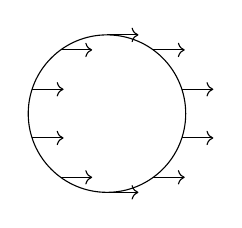
\begin{tikzpicture}
\draw (0,0) circle (1cm);
\foreach \rot in {36,72,...,360}{
\draw[->] ({sin(\rot)},{cos(\rot)}) -- +(.4,0);}
\end{tikzpicture}


\begin{tikzpicture}
\draw (0,0) -- (1,0) arc (0:300:1cm) -- cycle;
\end{tikzpicture}

If the connection is metric compatible, the \ueig{metric is parallel transported}. This means parallel transport preserves properties like norm, orthogonality etc.

\subsection{Geodesics}
Two way of seeing it:
\begin{enumerate}
\item Parallel transports it's own tangent vector
\item Shortest distance between two points.
\end{enumerate}

\subsubsection{As a curve that parallel transports it's tangent vector}
Setting directional covariant derivative of $\od{x^\mu}{\lambda}$ to zero gives
\[ \frac{D}{d\lambda}\od{x^\mu}{\lambda} = \boxed{ \od[2]{x^\mu}{\lambda} + \Gamma^\mu_{\rho\sigma}\od{x^\rho}{\lambda}\od{x^\sigma}{\lambda} = 0 } \]
This is the \textbf{geodesic equation}. In flat space using Cartesian coordinates, this reduces to the equation of straight lines.

Actually this procedure constrains the parametrisation of the curve. In general a curve may be thought of as a geodesic if it parallel transports the \emph{unit} tangent vector. The in formula above the norm of the tangent vector was also forced to be constant. This constrains the parametrisation to be an \udef{affine parameter}, which is a parameter of the form
\[ \lambda = a\tau + b \]
with $\tau$ the arc length (i.e. proper time) and $a$ and $b$ constants.

Now say $\alpha$ is an arbitrary parametrisation and $v(\alpha) = \left|\od{x^\mu}{\alpha}\right|$ the norm of the tangent vector $\od{x^\mu}{\alpha}$. The unit tangent vector is then $v^{-1}\od{x^\mu}{\alpha}$. Requiring that this be parallel transported gives
\begin{align}
\frac{D}{d\alpha}\left(v^{-1}\od{x^\mu}{\alpha}\right) &= \od{x^\rho}{\alpha}\nabla_\rho\left[v^{-1}\od{x^\mu}{\alpha}\right] \\
&= \od{x^\rho}{\alpha} \left[\partial_\rho \left(v^{-1}\od{x^\mu}{\alpha}\right) + \Gamma^\mu_{\rho\sigma}v^{-1}\od{x^\sigma}{\alpha}\right] \\
&= \od{x^\rho}{\alpha} \left[\od{x^\mu}{\alpha}\partial_\rho v^{-1} + v^{-1}\partial_\rho \od{x^\mu}{\alpha} + \Gamma^\mu_{\rho\sigma}v^{-1}\od{x^\sigma}{\alpha}\right] = 0.
\end{align}
Multiplying both sides by $v$ gives
\[ 0 = \od{x^\mu}{\alpha}v\od{x^\rho}{\alpha}\partial_\rho v^{-1} + \od[2]{x^\mu}{\alpha} + \Gamma^\mu_{\rho\sigma}\od{x^\rho}{\alpha}\od{x^\sigma}{\alpha} \]
which is the geodesic equation derived above plus an extra term of the form $f(\alpha)\od{x^\mu}{\alpha}$, with
\begin{align}
f(\alpha) &= v \od{v^{-1}}{\alpha} \\
&= -v^{-1}\od{v}{\alpha} \\
&= - \left(\od[2]{\tau}{\alpha}\right)\left(\od{\tau}{\alpha}\right)^{-1}
\end{align}
using $v = \od{\tau}{\alpha}$, because the proper time is the arc length (TODO rephrase?). The factor $f(\alpha)$ is obviously zero for affine parameters.

For timelike paths we can write the geodesic equation in terms of the four-velocity $u^\mu = \od{x^\mu}{\tau}$:
\[ u^\lambda\nabla_\lambda u^\mu = 0 \]

For massive particles the four-momentum $p^\mu$ is $mu^\mu$, making this equivalent to
\[ p^\lambda\nabla_\lambda p^\mu = 0 \]

\subsubsection{As the shortest distance between two points}
\paragraph{For timelike paths.} Consider the proper time functional for a timelike path parametrised by $\lambda$:
\[ \tau_{AB} = \int \left(-g_{\mu\nu} \od{x^\mu}{\lambda}\od{x^\nu}{\lambda}\right)^{1/2} \diff{\lambda} \]
We want to find the stationary paths, with $\delta \tau = 0$. Computing the variation and setting $f = g_{\mu\nu} \od{x^\mu}{\lambda}\od{x^\nu}{\lambda}$ gives
\begin{align}
\delta \tau &= \int \delta\sqrt{-f}\diff{\lambda} \\
&= -\int \frac{1}{2}(-f)^{-1/2}\delta f \diff{\lambda}.
\end{align}

Now we can reparametrise the path, taking the proper time as the new parameter. This means the tangent vector is the four-velocity $u^\mu$, which fixes $f$
\[ f = g_{\mu\nu} \od{x^\mu}{\tau}\od{x^\nu}{\tau} = g_{\mu\nu}u^\mu u^\nu = -1, \]
so
\[ \delta \tau = - \frac{1}{2}\int\delta f \diff{\tau} \]

This means stationary paths of the proper time functional are also stationary paths of the simpler integral
\[ I = \frac{1}{2}\int f \diff{\tau} = \frac{1}{2}\int g_{\mu\nu} \od{x^\mu}{\tau}\od{x^\nu}{\tau} \]
and vice versa.

We can explicitly vary this integral with (TODO why)
\[ \begin{cases}
x^\mu \to x^\mu _ \delta x^\mu \\
g_{\mu\nu} \to g_{\mu\nu} + (\partial_\sigma g_{\mu\nu})\delta x^\sigma.
\end{cases} \]
Plugging this into the expression for $I$ and keeping only terms that are first order in $\delta x^\mu$, we get
\[ \delta I = \frac{1}{2}\int \left[\partial_\sigma g_{\mu\nu}\od{x^\mu}{\tau}\od{x^\nu}{\tau}\delta x^\sigma + g_{\mu\nu}\od{(\delta x^\mu)}{\tau}\od{x^\nu}{\tau} +g_{\mu\nu}\od{x^\mu}{\tau}\od{(\delta x^\nu)}{\tau}\right]\diff{\tau} \]
The last two terms can be integrated by parts; for example,
\begin{align}
\int \left[ g_{\mu\nu}\od{x^\mu}{\tau}\od{(\delta x^\nu)}{\tau} \right]\diff{\tau} &= \left. g_{\mu\nu}\od{x^\mu}{\tau}\delta x^\nu \right|_\text{at boundary} - \int \od{}{\tau}\left(g_{\mu\nu}\od{x^\mu}{\tau}\right)\delta x^\nu \diff{\tau} \\
&= - \int \left[g_{\mu\nu} \od[2]{x^\mu}{\tau} + \od{g_{\mu\nu}}{\tau}\od{x^\mu}{\tau}\right]\delta x^\nu \diff{\tau} \\
&= - \int \left[g_{\mu\nu} \od[2]{x^\mu}{\tau} + \partial_\sigma g_{\mu\nu}\od{x^\sigma}{\tau}\od{x^\mu}{\tau}\right]\delta x^\nu \diff{\tau}
\end{align}
where we have used that $\delta x^\nu$ vanishes at the boundary.

The total variation is then
\[ \delta I = - \int \left[g_{\mu\sigma}\od[2]{x^\mu}{\tau} + \frac{1}{2}\left(\partial_\mu g_{\nu\sigma} + \partial_\nu g_{\sigma\mu} - \partial_\sigma g_{\mu\nu}\right)\od{x^\mu}{\tau}\od{x^\nu}{\tau}\right]\delta x^\sigma \diff{\tau}. \]
Since we are searching for stationary points, we want $\delta I$ to vanish for any variation $\delta x^\sigma$. This implies that the expression inside the square brackets must vanish. Multiplying it with the inverse metric $g^{\rho\sigma}$ yields
\[ \od[2]{x^\rho}{\tau} + \frac{1}{2}g^{\rho\sigma}\left(\partial_\mu g_{\nu\sigma} + \partial_\nu g_{\sigma\mu} - \partial_\sigma g_{\mu\nu}\right)\od{x^\mu}{\tau}\od{x^\nu}{\tau} = 0 \]
Which is exactly the geodesic equation with the Christoffel symbols as the connection.

This procedure provides a convenient way to calculate the Christoffel symbols for a given metric: by explicitly varying the integral $I$ with the metric of interest plugged in.

\paragraph{Null geodesics.} The geodesic formula was found using a very specific parametrisation, which is not a problem because all regular curves can be arc parametrised. Unfortunately we also restricted ourselves to timelike paths, because for null paths $\tau = 0$.

Now the geodesic equation derived above is still perfectly valid, even if $\tau$ can no longer be considered a valid parameter. An affine parameter is now any parameter such that the geodesic equation is satisfied, but now there is no special one. They are all related by the fact that if $\lambda$ is an affine parameter, any parameter of the form $a\lambda + b$ is as well. 

It is often convenient to normalise the affine parameter $\lambda$ along a null geodesic such that
\[ p^\mu = \od{x^\mu}{\lambda} \]

\paragraph{Timelike geodesics are maxima.} Locally that is. We can see that this is true because any timelike path can be arbitrarily well approximated by a null curve.

\subsubsection{Exponential map}
TODO

Geodesically incomplete

Riemann normal coordinates

\subsection{Riemann curvature tensor}
We now want an object that embodies our idea of curvature. Seeing as we are going to define a new object to fit out intuition, we need to flesh it out a bit first. We begin by naming some properties of flat spacetime:
\begin{itemize}
\item Parallel transport around a closed loop leaves vectors unchanged;
\item Covariant derivatives of tensors commute;
\item Initially parallel geodesics remain parallel.
\end{itemize}
TODO motivation.
\udef{Riemann tensor $\tensor{\mathcal{R}}{^\rho_{\sigma\mu\nu}}$} is a $(1,3)$-tensor. It is antisymmetric in the last two indices.

\begin{align}
[\nabla_\mu,\nabla_\nu]V^\rho &= \nabla_\mu\nabla_\nu V^\rho - \nabla_\nu\nabla_\mu V^\rho \\
&= \left(\partial_\mu(\nabla_\nu V^\rho) - \Gamma^\lambda_{\mu\nu}\nabla_\lambda V^\rho + \Gamma^\rho_{\mu\sigma}\nabla_\nu V^\rho \right) - \left(\partial_\nu(\nabla_\mu V^\rho) - \Gamma^\lambda_{\nu\mu}\nabla_\lambda V^\rho + \Gamma^\rho_{\nu\sigma}\nabla_\mu V^\rho \right) \\
&= 2\left(\partial_{[\mu}(\nabla_{\nu]} V^\rho) - \Gamma^\lambda_{[\mu\nu]}\nabla_\lambda V^\rho + \Gamma^\rho_{[\mu|\sigma|}\nabla_{\nu]} V^\rho \right) \\
&= 2\left(\partial_{[\mu}\partial_{\nu]} V^\rho + \partial_{[\mu}(\Gamma^\rho_{\nu]\sigma} V^\sigma) - \Gamma^\lambda_{[\mu\nu]}\nabla_\lambda V^\rho + \Gamma^\rho_{[\mu|\sigma|}\partial_{\nu]} V^\sigma + \Gamma^\rho_{[\mu|\sigma|}\Gamma^\rho_{\nu]\sigma} V^\sigma \right) \\
&= \cancel{[\partial_{\mu}, \partial_{\nu}] V^\rho} + 2\left(\partial_{[\mu}(\Gamma^\rho_{\nu]\sigma} V^\sigma) - \Gamma^\lambda_{[\mu\nu]}\nabla_\lambda V^\rho + \Gamma^\rho_{[\mu|\sigma|}\partial_{\nu]} V^\sigma + \Gamma^\rho_{[\mu|\sigma|}\Gamma^\rho_{\nu]\sigma} V^\sigma \right) \\
&= 2\left(\partial_{[\mu}(\Gamma^\rho_{\nu]\sigma}) V^\sigma + \cancel{\partial_{[\mu}( V^\sigma)\Gamma^\rho_{\nu]\sigma}} - \Gamma^\lambda_{[\mu\nu]}\nabla_\lambda V^\rho + \cancel{\Gamma^\rho_{[\mu|\sigma|}\partial_{\nu]} V^\sigma} + \Gamma^\rho_{[\mu|\sigma|}\Gamma^\rho_{\nu]\sigma} V^\sigma \right) \\
&= 2\left(\partial_{[\mu}\Gamma^\rho_{\nu]\sigma} + \Gamma^\rho_{[\mu|\sigma|}\Gamma^\rho_{\nu]\sigma} \right) V^\sigma - 2\Gamma^\lambda_{[\mu\nu]}\nabla_\lambda V^\rho \\
&= \left(\partial_{\mu}\Gamma^\rho_{\nu\sigma} - \partial_{\nu}\Gamma^\rho_{\mu\sigma} + \Gamma^\rho_{\mu\sigma}\Gamma^\rho_{\nu\sigma} - \Gamma^\rho_{\nu\sigma}\Gamma^\rho_{\mu\sigma} \right) V^\sigma - \tensor{T}{^\lambda_{\mu\nu}}\nabla_\lambda V^\rho \\
&\equiv \tensor{\mathcal{R}}{^\rho_{\mu\nu\sigma}}V^\sigma - \tensor{T}{^\lambda_{\mu\nu}}\nabla_\lambda V^\rho
\end{align}

Where $[\;,\;]$ is the antisymmetrisation, $[\mu|\sigma|\nu]$ means that only $\mu$ and $\nu$ are antisymmetrised and $T$ is the torsion tensor. So the Riemann tensor is identified as
\[ \boxed{\tensor{\mathcal{R}}{^\rho_{\mu\nu\sigma}} \equiv \partial_{\mu}\Gamma^\rho_{\nu\sigma} - \partial_{\nu}\Gamma^\rho_{\mu\sigma} + \Gamma^\rho_{\mu\sigma}\Gamma^\rho_{\nu\sigma} - \Gamma^\rho_{\nu\sigma}\Gamma^\rho_{\mu\sigma}} \]

\subsubsection{Properties of the curvature tensor}
To investigate the properties of the Riemann tensor, the upper index is lowered
\[ \mathcal{R}_{\rho\sigma\mu\nu} = g_{\rho\lambda}\tensor{\mathcal{R}}{^\lambda_{\sigma\mu\nu}} \]
and an explicit expression is obtained in locally inertial coordinates. In locally inertial coordinates the metric and its first derivatives vanish, so the Christoffel symbols do as well, but not their derivatives.
\begin{align}
\mathcal{R}_{\hat{\rho}\hat{\sigma}\hat{\mu}\hat{\nu}} &= g_{\hat{\rho}\hat{\lambda}} \left(\partial_{\hat{\mu}}\Gamma^{\hat{\lambda}}_{\hat{\nu}\hat{\sigma}} - \partial_{\hat{\nu}}\Gamma^{\hat{\lambda}}_{\hat{\mu}\hat{\sigma}}\right) \\
&= \frac{1}{2}g_{\hat{\rho}\hat{\lambda}}g^{\hat{\lambda}\hat{\tau}}\left[\left(\partial_{\hat{\mu}}\partial_{\hat{\nu}}g_{\hat{\sigma}\hat{\tau}} + \partial_{\hat{\mu}}\partial_{\hat{\sigma}}g_{\hat{\tau}\hat{\nu}} - \partial_{\hat{\mu}}\partial_{\hat{\tau}}g_{\hat{\nu}\hat{\sigma}}\right) - \left(\partial_{\hat{\nu}}\partial_{\hat{\mu}}g_{\hat{\sigma}\hat{\tau}} + \partial_{\hat{\nu}}\partial_{\hat{\sigma}}g_{\hat{\tau}\hat{\mu}} - \partial_{\hat{\nu}}\partial_{\hat{\tau}}g_{\hat{\mu}\hat{\sigma}}\right)\right] \\
&= \frac{1}{2}\left[\partial_{\hat{\mu}}\partial_{\hat{\sigma}}g_{\hat{\rho}\hat{\nu}} - \partial_{\hat{\mu}}\partial_{\hat{\rho}}g_{\hat{\nu}\hat{\sigma}} - \partial_{\hat{\nu}}\partial_{\hat{\sigma}}g_{\hat{\rho}\hat{\mu}} + \partial_{\hat{\nu}}\partial_{\hat{\rho}}g_{\hat{\mu}\hat{\sigma}}\right]
\end{align}
This derivation was done in a special coordinate system, but all tensorial equations that follow from it must be true in any coordinate system. A few such equations are now listed:
\begin{enumerate}
\item The Riemann tensor is antisymmetric in its first two indices.
\[ \boxed{ \mathcal{R}_{\rho\sigma\mu\nu} = - \mathcal{R}_{\sigma\rho\mu\nu} } \]
\item The Riemann tensor is antisymmetric in its last two indices.
\[ \boxed{ \mathcal{R}_{\rho\sigma\mu\nu} = - \mathcal{R}_{\rho\sigma\nu\mu} } \]
\item The Riemann tensor is invariant under exchange of the first and last pair of indices.
\[ \boxed{ \mathcal{R}_{\rho\sigma\mu\nu} = \mathcal{R}_{\mu\nu\rho\sigma} } \]
\item Thus sum of cyclic permutations of the last three indices vanishes.
\[ \mathcal{R}_{\rho\sigma\mu\nu} + \mathcal{R}_{\rho\mu\nu\sigma} + \mathcal{R}_{\rho\nu\sigma\mu} = 0 \]
This is equivalent to the vanishing of the antisymmetric part of the last three indices.
\[ \boxed{  \mathcal{R}_{\rho[\sigma\mu\nu]} = 0 } \]
\end{enumerate}
\paragraph{Number of parameters.} TODO
\paragraph{Bianchi identity.} TODO
\[ \nabla_{[\lambda}\mathcal{R}_{\rho\sigma]\mu\nu} = 0 \]

\subsubsection{Derived quantities}
Tricks for decomposition: taking contractions and taking (anti)symmetric parts.

\paragraph{Ricci tensor.} This \udef{Ricci tensor} is defined as
\[ \mathcal{R}_{\mu\nu} \equiv \tensor{\mathcal{R}}{^\lambda_{\mu\lambda\nu}}. \]
The Ricci tensor associated with the Christoffel connection is automatically symmetric:
\begin{align}
\mathcal{R}_{\mu\nu} &= g^{\rho\lambda}\mathcal{R}_{\rho\mu\lambda\nu} = g^{\rho\lambda}\mathcal{R}_{\lambda\nu\rho\mu} = \tensor{\mathcal{R}}{^\rho_{\nu\rho\mu}} \\
&= \mathcal{R}_{\nu\mu}
\end{align}
The trace of the Ricci tensor is called the \udef{Ricci scalar} (or curvature scalar):
\[ R \equiv \tensor{\mathcal{R}}{^\mu_\mu} = g^{\mu\nu}\mathcal{R}_{\mu\nu} \]

Now a useful form of the Bianchi identity can be obtained by multiplying it by $3g^{\nu\sigma}g^{\mu\lambda}$:
\begin{align}
0 &= 3g^{\nu\sigma}g^{\mu\lambda}\nabla_{[\lambda}\mathcal{R}_{\rho\sigma]\mu\nu} \\
&= \frac{3g^{\nu\sigma}g^{\mu\lambda}}{6!}\left[\left(\nabla_{\lambda}\mathcal{R}_{\rho\sigma\mu\nu} + \nabla_{\rho}\mathcal{R}_{\sigma\lambda\mu\nu} + \nabla_{\sigma}\mathcal{R}_{\lambda\rho\mu\nu}\right) - \left(\nabla_{\lambda}\mathcal{R}_{\sigma\rho\mu\nu} + \nabla_{\rho}\mathcal{R}_{\lambda\sigma\mu\nu} + \nabla_{\sigma}\mathcal{R}_{\rho\lambda\mu\nu}\right)\right] \\
&= g^{\nu\sigma}g^{\mu\lambda}\left[\nabla_{\lambda}\mathcal{R}_{\rho\sigma\mu\nu} + \nabla_{\rho}\mathcal{R}_{\sigma\lambda\mu\nu} + \nabla_{\sigma}\mathcal{R}_{\lambda\rho\mu\nu}\right] \\
&= \nabla^\mu\mathcal{R}_{\rho\mu} - \nabla_\rho R + \nabla^\nu\mathcal{R}_{\rho\nu}
\end{align}
or
\[ \boxed{\nabla^\mu\mathcal{R}_{\rho\mu} = \frac{1}{2}\nabla_\rho R.} \]


\paragraph{Weyl tensor.} TODO Why. In $n$ dimensions the \udef{Weyl tensor} is given by
\[ C_{\rho\sigma\mu\nu} \equiv \mathcal{R}_{\rho\sigma\mu\nu} - \frac{2}{n-2}\left(g{\rho[\mu}\mathcal{R}_{\nu]\sigma} - g{\sigma[\mu}\mathcal{R}_{\nu]\rho}\right) + \frac{2}{(n-1)(n-2)}g{\rho[\mu}\mathcal{R}_{\nu]\sigma} \]
TODO properties.

\paragraph{Einstein tensor.} The \udef{Einstein tensor} is defined as
\[ G_{\mu\nu} \equiv \mathcal{R}_{\mu\nu} - \frac{1}{2}Rg_{\mu\nu}. \]
Now the Bianchi identity reduces to
\[ \boxed{\nabla^{\mu}G_{\mu\nu} = 0} \]


\section{Isometries}
\subsection{About isometries}
TODO post geometry.
\[ g'_{\mu\nu}(y) = g_{\mu\nu}(y) \]

Symmetries of arbitrary tensor fields.
\subsection{Lie derivatives}
In general $g_{\mu\nu}(x_p)$ is different from $g_{\mu\nu}(x_q)$. Are there directions we can move in on the manifold so that the metric (or any other function on the manifold) doesn't change.
So we want
\[ g_{\mu\nu}(\tilde{x}) = \pd{x^\rho}{\tilde{x}{^\mu}}\pd{x^\sigma}{\tilde{x}{^\nu}}g_{\rho\sigma}(x) \]
to equal the original metric.

We consider an infinitessimal transformation:
\[ \tilde{x}^\mu = x^\mu+\epsilon V^\mu \]
\[ \delta y^\mu = \pd{y^\mu}{x^\nu}\delta x^\nu \]

\subsubsection{Lie derivative on a scalar}
We are comparing
\[  \begin{cases}
\phi(\tilde{x}) = \phi(x + \epsilon V) = \phi(x) + \epsilon V^\mu\partial_\mu \phi(x) + \mathcal{O}(\epsilon^2) \\
\tilde{\phi}(\tilde{x}) = \phi(x)
\end{cases}\]

\begin{align}
L_V\phi &\equiv \lim_{\epsilon\to 0}\frac{\phi(\tilde{x}) - \tilde{\phi}(\tilde{x})}{\epsilon} \\
&= \lim_{\epsilon\to 0}\frac{\phi(x+\epsilon V^\mu)-\phi(x)}{\epsilon} \\
&= \lim_{\epsilon\to 0}\frac{\cancel{\phi(x)}+\epsilon V^\mu\partial_\mu\phi(x)+\mathcal{O}(\epsilon^2)-\cancel{\phi(x)}}{\epsilon} \\
&= V^\mu\partial_\mu\phi(x)
\end{align}

Ordinary directional derivative.

In general:
\[ L_V: (p,q) \text{forms} \to (p,q) \text{forms} \]

\subsubsection{Lie derivative of a vector field}
Again we define
\[ L_VW^\mu \equiv \lim_{\epsilon\to 0}\frac{W^\mu(\tilde{x}) - \tilde{W^\mu}(\tilde{x})}{\epsilon} \]
Again we are comparing two quantities
\begin{align}
W(\tilde{x}) &= W(x + \epsilon V) = W(x) + \epsilon V^\mu\partial_\mu W(x) + \mathcal{O}(\epsilon^2) \\
\tilde{W}(\tilde{x}) &= \pd{\tilde{x}^\mu}{x^\nu}W^\nu (x) \\
&= \pd{(x^\mu+\epsilon V^\mu)}{x^\nu}W^\nu (x) \\
&= \left(\delta^\mu_\nu+\epsilon \pd{V^\mu}{x^\nu}\right)W^\nu (x) \\
&= W^\mu (x)+\epsilon W^\nu (x)\partial_\nu V^\mu
\end{align}

Putting everything together, we get
\[ L_V W^\mu = V^\nu\partial_\nu W^\mu - W^\nu \partial_\nu V^\mu \]

Normal derivative not covariant, but here same as covariant derivative (extra bits cancel).

Not defined with respect to any particular metric.

Some properties:
\begin{itemize}
\item Partial derivatives can be replaced by covariant ones.
\item The Lie derivative is antisymmetric in $V$ and $W$ and defines a commutator
\[ [V,W]^\mu \equiv L_VW^\mu = - L_WV^\mu \]
This satisfies the Jacobi identity 
\[ [V,[W,X]]^\mu + [X,[V,W]]^\mu + [W,[X,V]]^\mu \]
and thus is a Lie bracket.  The Jacobi identity is equivalent to
\[ L_V[W,X]^\mu = [L_VW,X]^\mu + [W,L_VX]^\mu \]
\end{itemize}


\subsubsection{Lie derivative of other tensor fields}
The definitions above are readily generalised
\[ \tilde{x}^\mu(x) = x^\mu +\epsilon V^\mu(x) \]
\[ L_VT = \lim_{\epsilon\to 0} \frac{T(\tilde{x})-\tilde{T}(\tilde{x})}{\epsilon} \]
where we need
\[ \pd{\tilde{x}^\mu}{x^\rho} = \delta^\mu_\rho + \epsilon \partial_\rho V^\mu + \mathcal{O}(\epsilon^2) \qquad \text{and}\qquad \pd{x^\mu}{\tilde{x}{^\rho}} = \delta^\mu_\rho - \epsilon \partial_\rho V^\mu + \mathcal{O}(\epsilon^2) \]

Again partial derivatives can be replaced by covariant derivatives. We illustrate with a $(0,2)$-tensor $T_{\mu\nu}$.
\[ \begin{cases}
T_{\mu\nu}(\tilde{x}) = T_{\mu\nu}(x) + \epsilon V^\rho\partial_\rho T_{\mu\nu}+ \mathcal{O}(\epsilon^2) \\
\tilde{T}_{\mu\nu}(\tilde{x}) = \pd{x^\mu}{\tilde{x}{^\mu}}\pd{x^\nu}{\tilde{x}{^\nu}}T_{\mu\nu} = T_{\mu\nu} - \epsilon\partial_\mu V^\rho T_{\rho\nu}(x) - \epsilon\partial_\nu V^\sigma T_{\mu\sigma} + \mathcal{O}(\epsilon^2)
\end{cases} \]
Filling this in gives
\begin{align}
L_V T_{\mu\nu} &= \lim_{\epsilon\to 0} \frac{T_{\mu\nu}(\tilde{x})-\tilde{T}_{\mu\nu}(\tilde{x})}{\epsilon} \\
&= \lim_{\epsilon\to 0} \frac{\cancel{T_{\mu\nu}(x)}+\epsilon V^\rho\partial_\rho T_{\mu\nu}+ \mathcal{O}(\epsilon^2)-\cancel{T_{\mu\nu}}+\epsilon T_{\rho\nu} \partial_\mu V^\rho +\epsilon T_{\mu\sigma} \partial_\nu V^\sigma + \mathcal{O}(\epsilon^2)}{\epsilon} \\
&= V^\rho\partial_\rho T_{\mu\nu} + T_{\rho\nu} \partial_\mu V^\rho + T_{\mu\rho} \partial_\nu V^\rho \\
&= V^\rho \left(\nabla_\rho T + \Gamma^\lambda_{\rho \mu}T_{\lambda \nu} + \Gamma^\lambda_{\rho \nu}T_{\mu \lambda} \right) + T_{\rho\nu} \left(\nabla_\mu V^\rho - \Gamma^\rho_{\mu\lambda}V^\lambda\right) + T_{\mu\rho} \left(\nabla_\nu V^\rho - \Gamma^\rho_{\nu\lambda}V^\lambda\right) \\
&= V^\rho\nabla_\rho T + T_{\rho\nu}\nabla_\mu V^\rho + T_{\mu\rho}\nabla_\nu V^\rho + \left(\Gamma^\lambda_{\rho \mu}V^\rho T_{\lambda \nu} - \Gamma^\rho_{\mu\lambda}V^\lambda T_{\rho\nu}\right) + \left(\Gamma^\lambda_{\rho \nu}V^\rho T_{\mu \lambda} - \Gamma^\rho_{\nu\lambda}V^\lambda T_{\mu\rho}\right) \\
&= V^\rho\nabla_\rho T + T_{\rho\nu}\nabla_\mu V^\rho + T_{\mu\rho}\nabla_\nu V^\rho
\end{align}

Isometries from an algebra
\[ \left[L_V,L_W\right] = L_{[V,W]} \]
Enough to verify scalars and vectors.

\subsubsection{Lie derivative of tensor densities}
TODO

\subsection{Killing vectors}
The Lie derivative of the metric tensor. This is $(0,2)$-tensor, so the formula is the one given above.
Due to metric compatibility, the first term is zero
\begin{align}
L_V g_{\mu\nu} &= V^\rho\nabla_\rho g_{\mu\nu} + g_{\lambda\nu}\nabla_\mu V^\lambda + g_{\mu\lambda}\nabla_\nu V^\lambda \\
&= g_{\lambda\nu}\nabla_\mu V^\lambda + g_{\mu\lambda}\nabla_\nu V^\lambda \\
&= \nabla_\mu V_\nu + \nabla_\nu V_\nu \\
\end{align}

An infinitesimal coordinate transformation is a symmetry of the metric if $L_V g_{\mu\nu} = 0$, which is equivalent to requiring $V$ to satisfy the equations
\[ \nabla_\mu V_\nu + \nabla_\nu V_\nu = 0 = \nabla_{(\mu} V_{\nu)}. \]
Such vectors are called \udef{Killing vectors}. These equations are equivalent to
\[ \nabla_\mu V_\nu = \nabla_{[\mu}V_{\nu]} \]


Properties:
\begin{enumerate}
\item Killing vectors form a Lie algebra. If $V$ and $W$ are Killing vectors, i.e. $L_Vg_{\mu\nu} = L_Wg_{\mu\nu} = 0$, then $[V,W]$ is a Killing vector because
\[ L_{[V,W]}g_{\mu\nu} = L_VL_Wg_{\mu\nu} - L_WL_V g_{\mu\nu} = 0  \]
\item If all the components of the metric are independent of a particular coordinate, say $y$
\[ \partial_y g_{\mu\nu} \qquad \forall \mu,\nu \]
Then $V=\partial_y$ is a Killing vector. A coordinate system in which a Killing vector is a partial derivative is said to be \textit{adapted} to the Killing vector (or isometry) in question. TODO derive Killing equations from this.
\item Two Killing vectors commute if and only if there is a coordinate system that is adapted to both of them.
\end{enumerate}

You can use the equations in 2 ways:
\begin{itemize}
\item Impose symmetries on the metric.
\item Find the Killing vectors for a given metric, which gives the symmetries
\end{itemize}

\begin{example}
Algebra of Killing vectors in Minkowski and two-sphere.
\end{example}

\subsection{Conserved quantities}
\subsubsection{Conserved charges along geodesics}
Let $K^\mu$ be a Killing vector field and $x^\mu(\tau)$ a geodesic with four-velocity $x^\mu$. Then the quantity
\[ Q_K = K_\mu u^\mu \]
is constant along the geodesic. Indeed,
\begin{align}
\od{}{\tau}Q_K = \od{K_\mu u^\mu}{\tau} &= u^\mu \od{K_\mu}{\tau} + K_\mu \od{}{\tau}u^\mu \\
&= u^\mu u^\nu \nabla_\nu K_\mu + 0\\
&= \frac{1}{2}\left(\nabla_\nu K_\mu + \nabla_\mu K_\nu\right)u^\mu u^\nu = 0
\end{align}
where the last equality is due to the Killing equations.

\subsubsection{Conserved currents from the energy-momentum tensor}
Let $K^\mu$ be a Killing vector field and $T^{\mu\nu}$ the covariantly conserved symmetric energy-momentum tensor ($\nabla_\mu T^{\mu\nu} = 0$). Then the current
\[ J_K^\mu = T^{\mu\nu}K_\nu \]
is covariantly conserved. Indeed,
\begin{align}
\nabla_\mu J^\mu_K &= (\nabla_\mu T^{\mu\nu})K_\nu + T^{\mu\nu} \nabla_\mu K_\nu \\
&= 0 + \frac{1}{2}T^{\mu\nu}\left(\nabla_\mu K_\nu + \nabla_\nu K_\mu\right) = 0
\end{align}

\subsubsection{Komar currents}
The Einstein tensor is symmetric and conserved (from the Bianchi identity), so we have the conserved current
\[ J^\mu_1 = \tensor{G}{^\mu_\nu}K^\nu =  \]

\subsection{Killing tensors}

\subsubsection{Killing(-Stäckel) tensors}
A \udef{Killing tensor $K_{\beta_1\ldots\beta_n}$} is a totally symmetric tensor satisfying
\[ \nabla_{(\alpha}K_{\beta_1\ldots\beta_n)} = 0. \]

The charge
\[ Q_K = K_{\beta_1\ldots\beta_n}u^{\beta_1}\ldots u^{\beta_n} \]
is constant along the geodesic.

\subsubsection{Killing-Yano tensors}
A \udef{Killing-Yano tensor $Y_{\beta_1\ldots\beta_n}$} is a totally anti-symmetric tensor satisfying
\[ \nabla_{(\alpha} Y_{\beta_1)\ldots\beta_n} = 0 \qquad \text{or, equivalenty} \qquad \nabla_\alpha Y_{\beta_1\ldots\beta_n} = \nabla_{[\alpha}Y_{\beta_1\ldots\beta_n]} \]

The tensorial charges
\[ Z_{\beta_1\ldots\beta_{n-1}} = u^\beta Y_{\beta\beta_1\ldots\beta_{n-1}} \]
are conserved along geodesics.


\subsubsection{Symmetries and conserved charges (Komar integrals)}
\subsubsection{Conservation laws}
Conservation laws
\begin{itemize}
\item for geodesics
\item for spacetime
\end{itemize}

\[ Q = V^\mu \od{x^\nu}{\tau}g_{\mu\nu} \]
$\od{}{\tau}Q$ if $V$ is Killing and $\dot{x}^\mu$ is a geodesic.
\begin{align}
\od{}{\tau}Q = \od{}{\tau}\left(V_\mu\dot{x}^\mu\right) &= \left(\frac{DV_\mu}{D\tau}\right)\dot{x}^\mu + V_\mu \frac{D\dot{x}^\mu}{\tau} \\
&= \underbrace{\dot{x}^\rho D_\rho V_\mu \dot{x}^\mu}_{=0 \text{because Killing}} + \underbrace{V_\mu \frac{D\dot{x}^\mu}{D\tau}}_{=0 \text{geodesic}}
\end{align}

\subsection{Maximally symmetric spaces}
In D=4, maximally 10 symmetries. Minkowski maximally symmetric, but not uniquely so.
(Depends on number of killing vectors (which also form an algebra and can commute or not))

\[ K^\mu(x) \text{Killing} \quad \Leftrightarrow \quad D_{[\mu}K_{\nu]} = 0 \]
\[ K_\mu(x) = K_\mu(x^*) + \partial_\nu K_\mu(x^*)(x^\nu-x^{\nu*}) + \frac{1}{2}\partial_\rho\partial_\nu K_\mu(x^*)(x^\nu-x^{\nu *}(x^\rho - x^{\rho*}) + \ldots \]

\[ D_\mu K_\nu = \partial_\mu K_\nu - \Gamma^\rho_{\mu\nu}K_\rho \]
\[ \partial_\nu K_\mu(x^*) = D_\nu K_\mu(x^*) + \Gamma_{\nu\mu}^{\;\;\rho}K_\rho(x^*) \]
With
\[ D_\nu K_\mu(x^*) = \underbrace{\cancel{D_{(\nu}K_{\mu)}}}_{0 \text{because Killing}} + D_{[\nu}K_{\mu]}(x^*) \]
So
\[ \frac{D(D-1)}{2} \qquad \text{for} D=4 \quad \Rightarrow \quad 6 \text{coeff.} \]

Maximally symmetric:
\begin{itemize}
\item Minkowski: 4 translations, 6 Lorentz ($\Lambda = 0$)
\[ [P_\mu, P_\nu] = 0, \qquad [M_{\mu\nu}, P_\rho] = 2 \eta_{\rho[\mu}P_{\nu]}, \qquad [M_{\mu\nu}, M^{\rho\sigma}] = 4 \delta_{[\mu}^{\;\;[\rho}M_{\nu]}^{\;\;\sigma]} \]
\[M^{\mu\nu} = x^\mu\partial^\nu - x^\nu\partial^\mu \qquad G=\R^4 \rtimes \SO(1,3)\]
\item de Sitter $G = \SO(1,4)$ ($\Lambda>0$)
\item Anti-de Sitter $G=\SO(2,3)$
\end{itemize}
On a side note
\[ dS_4 \equiv \frac{\SO(1,4)}{\SO(1,3)} \qquad AdS_4 \equiv \frac{\SO(2,3)}{\SO(1,3)} \]
Confer:
\[ S^p = \frac{\SO(p+1)}{\SO(p)} \]

riemann normal coordinates + freely falling frames

\section{Conformal transformations}
\subsection{Conformal Killing vectors}
\[ L_C g_{\mu\nu} = \nabla_\mu C_\nu + \nabla_\nu C_\mu = 2\omega(x)g_{\mu\nu} \]

A Killing vector for a metric is at least a conformal Killing vector for any conformally rescaled metric.

\subsubsection{Conserved charges along null geodesics}
\[ Q_C = C_\mu u^\mu \]
\subsubsection{Conserved currents from the energy-momentum tensor}
energy-momentum tensor is traceless
\[ J_C^\mu = T^{\mu\nu}C_\nu \]

\subsection{Conformal Killing(-Yano) tensors}


\chapter{Lie groups and algebras}

\section{Lie Group}
A Lie group is a topological group that is also a differential manifold. This means we can apply differentials, which is of course very important. So important in fact that Sophus Lie called Lie groups infinitesimal groups when he first introduced them. Not only that, but it means we can consider tangent spaces, which will also be important later. TODO better justification

Bearing in mind the link between the topology and group properties explored in the section on topological groups, we quite naturally arrive at the following definition:
\begin{definition}
A \udef{Lie group} is a smooth manifold $G$ which is also a group and such that both the group product $G\times G \to G$ and the inverse map $G \to G$ are smooth.
\end{definition}

There is a particular type of Lie group that will be of particular importance to us, namely the matrix Lie group. In fact we will almost exclusively consider matrix Lie groups.

\subsection{Matrix Lie group}
For matrix groups there is a simpler condition to see whether it is a Lie group or not:
\begin{eigenschap}
All \ueig{closed subgroups} of $\GL(n, \C)$ are matrix Lie groups.
\end{eigenschap}
The condition that it be closed means that for every sequence in the Lie group the limit needs to be in the Lie group as well, if there is one. (Or you can say every Cauchy sequence in the Lie group has to have a limit in the Lie group). This is a technicality and is satisfied for most of the interesting subgroups of $\GL(n, \C)$. 

We have already seen that all subgroups of $\GL(n, \C)$ are topological groups. To prove the assertion then we must only verify that it is a smooth manifold. Because $\C^{n\times n}$ is a manifold and a matrix Lie group is a subset of $\C^{n\times n}$, the matrix Lie group inherits Hausdorffness and second-countability from $\C^{n\times n}$. To show it is smooth and locally homeomorphic to $\R^{m}$ in every point, we will explicitly construct such homeomorphisms using the matrix exponential.

\subsubsection{Exponential maps}
The homeomorphisms will be constructed based on the exponential map.
\[ \exp: \GL(n,\C) \to \GL(n,\C): X \mapsto e^X \]
This map is not a bijection, however if we restrict it to a neighbourhood of $\mathbb{0}$, it is locally a bijection. In fact it maps that neighbourhood to a neighbourhood of $\mathbb{1}$. More formally
\begin{eigenschap}
There exists a neighbourhood $U$ of $\mathbb{0}$ and a neighbourhood $V$ of $\mathbb{1}$ such that the exponential mapping takes $U$ homeomorphically onto $V$.
\end{eigenschap}
This result should not be surprising. For $X$ close to $\mathbb{0}$ we have the approximation $e^{X} \approx \mathbb{1} + X + \mathcal{O}(X^2)$. So for matrices in a small neighbourhood $U$ around $\mathbb{0}$ the exponential mapping can be seen as approximately linear, which is injective. In order to get surjectivity, we restrict the codomain of the mapping to the image of $U$ under the exponential mapping. This is a neighbourhood of $\mathbb{1}$ because $e^0 = \mathbb{1}$. 

We have obtained a bijection and because the matrix exponential is continuous, this restriction of it is also continuous. We would now like to show that the map maps open sets in our matrix Lie group, which we shall now call $G$, to open sets of $\R^{m}$. Unfortunately it doesn't. There is no reason why $\mathbb{0}$ or any matrices in $U$ should be elements of $G$. (Remember that the relevant group operation for matrix groups is the matrix multiplication, for which the neutral element is $\mathbb{1}$; the matrix $\mathbb{0}$ is of no particular importance in this context.) Being a group, the matrix Lie group must contain $\mathbb{1}$; being a topological group, it must contain a neighbourhood of $\mathbb{1}$; being a subspace of $\GL(n,\C)$ endowed with the subspace topology, the intersection of $V$ with that neighbourhood is an open set in $G$ which we will call $V'$.

So if we invert the restricted matrix exponential, we get a homeomorphism from \undline{one} neighbourhood of $G$ to $\GL(n,\C)$, which can then be composed with a homeomorphism to $\R^m$.

\begin{definition}
The inverse map $\exp^{-1}: V' \to U$ is called the \udef{logarithm}.
\end{definition}

From this we can construct a homeomorphism from a neighbourhood of any element $A$ of $G$. By multiplying each element of $V'$ with $A$ we get a neighbourhood $V_A$ of $A$. We define the following homeomorphism on $V_A$: multiply by $A^{-1}$ (this is bijective due to associativity of the group operation and continuous due to the definition of topological groups) and then send through the inverted, restricted matrix exponential. This composition of homeomorphisms is a homeomorphism. So for each element $A \in G$ we can find a neighbourhood $V_A$ that is homeomorphic to $\R^m$ thanks to this homeomorphism.

\begin{example}
TODO Finite Lie group
\end{example}


\subsubsection{Lie algebra of a matrix Lie group}
TODO: justification

\begin{definition}
Let $G$ be a matrix Lie group. The \udef{Lie algebra} of $G$, denoted $\mathfrak{g}$, is the set of all matrices $X_t$ such that $e^{itX_t}$ is in $G$ for all \undline{\textbf{real}} numbers $t$. We call the matrices $X_t$ \udef{generators} of the group.
\end{definition}

\begin{note}
Now here we have a complication. There are actually two conventions. The definition above is the convention most often used in physics. In the mathematics literature the Lie algebra in usually defined using $e^{tX_t}$, not $e^{itX_t}$. The physics convention gives rise to Hermitian generators in the algebras of $\U(n)$ and $\SU(n)$. This is useful because we are often interested in turning them into quantum operators, which correspond to observables only if they are Hermitian. The downside of this convention however is that it makes our life much more difficult in other places, and it even means that some definitions don't make any sense. In what follows we will generally be using the physics convention. We will however make use of the mathematics convention when the need arises. Also if there are interesting differences in the mathematics definition, we will mention those as well.
\end{note}

To try to grasp why the definition given above is useful, we introduce the notion of parametrization of group elements.
\subsubsection{Parametrization of group elements.}
When first introducing the matrix groups, we pointed out how the elements could be written in function of real parameters. We now make this notion more concrete and begin by defining a one-parameter subgroup.
\begin{definition}
A function $A : \R \to \GL(n, \C)$ is called a \udef{one-parameter subgroup} of $\GL(n, \C)$ if
\begin{enumerate}
\item $A$ is continuous,
\item $A(0) = \mathbb{1}_n$,
\item $A(t+s) = A(t)A(s)$ for all $t,s \in \R$.
\end{enumerate}
\end{definition}
If $A$ is a one-parameter subgroup of $\GL(n,\C)$, then it has the following property:
\begin{eigenschap}
There exists a unique $n\times n$ complex matrix $X$ such that
\[ A(t) = e^{tX} \]
\end{eigenschap}

So $X_t$ is in $\mathfrak{g}$ if and only if the one-parameter subgroup generated by $X_t$ lies in G. Conversely for any one-parameter subgroup that is a subgroup of G, there exists a generator and that generator is by definition part of the algebra.

Before continuing we shall consider some examples of algebras of matrix Lie groups. In general we shall call the algebra of a Lie group the lowercase version of the name of the Lie group. E.g., the Lie algebra of $\GL(n, \C)$ is $\glAlg(n,\C)$.

\begin{example}
\begin{enumerate}
\item If $X$ is any $n\times n$ complex matrix, then $e^{itX}$ is invertible. Thus the Lie algebra, $\glAlg(n,\C)$, of the invertible matrices, $\GL(n,\C)$, is the space of all complex $n\times n$ matrices.
\item If we use the mathematical convention, then the Lie algebra of $\GL(n,\R)$ is the space of all real $n\times n$ matrices, denoted $\glAlg(n,\R)$. To prove this we first remark that is $X$ is any real $n\times n$ matrix, then $e^{tX}$ will be invertible and real. Conversely, if $e^{tX}$ is real for all real $t$, then $X=\left.\od{}{t}e^{tX}\right|_{t=0}$ will also be real. Obviously in the physics convention the above no longer holds true.

\item The Lie algebra $\slAlg(n,\C)$ of $\SL(n,\C)$ is the space of all complex $n \times n$ matrices with zero trace. To prove this we use that
\[ \det(e^X) = e^{\Tr(X)}. \]
If $\Tr(X) = 0$, then $\det(e^{itX}) = 1$ for all real numbers $t$. On the other hand, if $X$ is any $n\times n$ matrix such that $\det(e^{itX}) =1$ for all $t$, then $e^{it\Tr(X)} = 1$ for all $t$. This means that $it\Tr(X)$ is an integer multiple of $2\pi i$ for all $t$, which is only possible if $\Tr(X) = 0$.

\item Lie algebra of $\U(N)$. If $X$ is to be a generator in our algebra, we need $e^{itX}$ to be unitary. So
\[ \left(e^{itX}\right)^\dagger = \left(e^{itX}\right)^{-1} = e^{-itX}. \]
We also have that
\[ \left(e^{itX}\right)^\dagger = e^{-itX^\dagger}. \]
Which gives us
\[ e^{-itX} = e^{-itX^\dagger}. \]
Differentiating at $t=0$ we see that the generators have to be Hermitian ($X = X^\dagger$).

We can also prove this by writing out the definition of the matrix exponential. 
\[ U(N) \ni U = e^{it_iX_i} \]
\begin{align}
\mathbb{1} = U^\dagger U &= (\mathbb{1}-it_i X_i^\dagger + \ldots )(\mathbb{1}+it_i X_i + \ldots) \\
&= \mathbb{1} + it_i(X_i^\dagger - X_i) + \ldots = \mathbb{1}
\end{align}
So we require the generators to be Hermitian matrices ($X_i^\dagger = X_i$). We have $N^2$ independent $X_i$ that are Hermitian. 
\[ \uAlg(N) = \{ H \in \GL(N,\C), H^\dagger = H \} \]
In the mathematics convention this condition becomes that the generators have to be skew-Hermitian, i.e. $X_i^\dagger = -X_i$.

\item Lie algebra of $\SU(N)$. Combining the arguments for the algebras of the unitary and special linear group, we see that the generators must be unitary and of trace zero. In other words the algebra is given by
\[ \suAlg(N) = \{ H\in\uAlg(N), \Tr[H] = 0 \} \]
and has dimension $N^2-1$.

For $N=2$ we have:
\[ \begin{cases}
\suAlg(2) = \{\sigma_1, \sigma_2, \sigma_3\} \\
\uAlg(2) = \{\sigma_1, \sigma_2, \sigma_3, \mathbb{1}\}
\end{cases} \]
Where
\[ \sigma_1 = \begin{pmatrix}
0 & 1 \\ 1 & 0
\end{pmatrix}, \qquad \sigma_2 = \begin{pmatrix}
0 & -i \\ i & 0
\end{pmatrix}, \qquad \sigma_3 = \begin{pmatrix}
1 & 0 \\ 0 & -1
\end{pmatrix}\]

\item Lie algebra of $\Ogroup(N)$. As explained above, if we want the algebra to be real, we need to make use of the mathematical convention. So $O=e^{t_iX_i}$.
\begin{align}
\mathbb{1} = O^\intercal O = e^{t_iX_i^\intercal}e^{t_iX_i} &= (\mathbb{1}+t_i X_i^\intercal + \ldots )(\mathbb{1}+t_i X_i + \ldots) \\
&= \mathbb{1} + t_i(X^\intercal_i + X_i) + \ldots
\end{align}
So we require the generators to be antisymmetric matrices ($X_i^\intercal = -X_i$).
\[ \oAlg(N) = \{ X \in \GL(N,\R), X^\intercal = -X \} = \soAlg(N) \]
The dimension of $\oAlg(N)$ is $\frac{N(N-1)}{2}$.
\end{enumerate}
\end{example}

The Lie algebra as defined above is in some way prototypical. I.e. when we make this notion more abstract, we want the abstract notion to behave in a similar fashion and have many of the same properties. Of course to do that we first need an idea of what properties these Lie algebras actually have. This is what we will be exploring next.

\begin{eigenschap}
If $G$ is a \textit{connected} matrix Lie group, then every $A \in G$ can be written in the form
\[ A = e^{X_1}e^{X_2}\ldots e^{X_m} \]
for some $X_1, X_2, \ldots, X_m$ in $\mathfrak{g}$
\end{eigenschap}

\begin{eigenschap}
Every continuous homomorphism between two matrix Lie groups is smooth.
\end{eigenschap}

\begin{eigenschap}
A matrix $X$ is in $\mathfrak{g}$ if and only if there exists a smooth curve $\gamma$ in $\C^{n\times n}$ such that
\begin{enumerate}
\item $\gamma(t)$ lies in $G$ for all $t$;
\item $\gamma(0) = \mathbb{1}$;
\item $\left.\od{\gamma}{t}\right|_{t=0} = X$
\end{enumerate}
Thus $\mathfrak{g}$ is the tangent space at the identity to $G$.
\end{eigenschap}


\begin{itemize}
\item If we assume $X \in \mathfrak{g}$, we can take $\gamma(t) = \exp(tX)$. This $\gamma(t)$ satisfies the points of the proposition above.
\item We now assume $\gamma(t)$ is a smooth curve in $G$ with $\gamma(0) = \mathbb{1}$.
\begin{align}\od{\gamma(t)}{t} &= \lim_{\delta t \to 0} \frac{\gamma(t+\delta t)-\gamma(t)}{\delta t} = \gamma(t)\left(\lim_{\delta t \to 0}\frac{\gamma(\delta t)-\gamma(0)}{\delta t}\right) \\ &= \gamma(t)\left.\od{\gamma}{t}\right|_{t=0} = \gamma(t)X \end{align}
From which we get that
\[ \gamma(t) = \exp{tX} \]
\end{itemize}

Now this is interesting, so interesting in fact that we use this last proposition to construct a general definition of a Lie algebra associated to a Lie group.

We can now also reintroduce the physics convention. We just divide all elements of any algebra by the imaginary unit $i$. The elements of this algebra may not be closed under the bracket operation, but that does not matter as we have a different definition to work from now: they are elements of the tangent space at identity to $G$, rescaled with a fractor $-i$.

We have already seen that in the mathematics convention the commutator belongs to the algebra (remembering to sum according to Einstein notation):
\[ [X_i, X_j] = f_{ij}^k X_k \]
Where we call $f_{ij}^k$ a \udef{structure constant} (with respect to the chosen basis of course). In the physics convention, we obviously need to deal with the factor $i$:
\[ [X_i, X_j] = if_{ij}^k X_k \]
\begin{eigenschap}
From the antisymmetry of the bracket we get:
\[ f^k_{ij} + f^k_{ji} = 0 \]
From the Jacobi identity we get:
\[ f^m_{ie}f^e_{jk} + f^m_{je}f^e_{ki} + f^m_{ke}f^e_{ij} = 0 \]
\end{eigenschap}

And lastly a final property of Lie algebras of matrix Lie groups follows straight from the \ueig{Baker-Campbell-Hausdorff formula}: 
\[ e^{A}e^{B} = e^C \qquad \text{with} \qquad C=A+B+\frac{1}{2}[A,B] + \frac{1}{12}([A,[A,B]]+[B,[B,A]]) + \ldots  \]
\begin{eigenschap}
To know the (local) structure of a Lie group close to the identity one \ueig{only} needs to know the commutator of the generators $[X_i,X_j]$
\end{eigenschap}

\section{Lie Algebra}
Again we will start by restricting our attention to Lie algebra's of matrix Lie groups. That way we can give some examples that will (hopefully) aid in the understanding of the general case.


\subsection{Definition}

\begin{eigenschap}
Let $G$ be a matrix Lie group, with Lie algebra $\mathfrak(g)$. Let $X$ and $Y$ be elements of $\mathfrak{g}$. Then
\begin{enumerate}
\item $sX \in \mathfrak{g}$, for all \undline{real} numbers $s$,
\item $X+Y \in \mathfrak{g}$,
\item $-i(XY - YX)\in \mathfrak{g}$.
\end{enumerate}
\end{eigenschap}
The first two points mean that the Lie algebra is actually a vector space over the \undline{real} numbers. This is important and serves as the crux of our first generalisation of Lie algebras, so we will have a quick look at the proofs of the statements above. 

\begin{enumerate}
\item This first point is fairly straightforward, since $e^{t(sX)} = e^{(ts)X}$, which must be in $G$ if $X$ is in $\mathfrak{g}$.
\item If $X$ and $Y$ commute, this is again immediate. If they don't however we need to do a little more work. We start from the Lie product formula:
\[ e^{t(X+Y)} = \lim_{m\to\infty} \left(e^{\frac{tX}{m}}e^{\frac{tY}{m}}\right)^m \]
Clearly if $X, Y \in \mathfrak{g}$,  for every $m$, $e^{\frac{tX}{m}}$ and $e^{\frac{tY}{m}}$ are elements of $G$. Since $G$ is a group, $\left(e^{\frac{tX}{m}}e^{\frac{tY}{m}}\right)^m$ is in $G$. Now because $G$ is a matrix Lie group, and thus \textit{closed} in $\GL(n, \C)$, the limit must also be in $G$. (If that is the limit is in $\GL(n, \C)$, which it is because $e^{t(X+Y)}$ is invertible). This shows that $X+Y$ is in $\mathfrak{g}$.
\item The third point follows from the product rule of the differential operator. Alternatively we can use the Baker-Campbell-Hausdorff formula:
\[e^{tX}e^{sY} = e^{tX+sY+ \frac{ts}{2}[X,Y] + \ldots}\]
This together with the first two points shows the third point.
\end{enumerate}

We have shown that the Lie algebra is a vector space over the real numbers, but crucially a Lie algebra is in general not a vector space over complex numbers, even if it consists of matrices with complex entries. For an example we consider the algebra $\suAlg(n)$, which consists of Hermitian matrices with zero trace. Assume $X$ is such a matrix. Now because $(iX)^\dagger = -iX^\dagger = -iX$, $iX$ is not Hermitian. As a consequence it cannot be an element of $\suAlg(n)$ and thus $\suAlg(n)$ is not a complex vector space.

If we follow the mathematical definition, the third point becomes $XY - YX \in \mathfrak{g}$. This will be important later. In fact it's so important we will give it name.
\begin{definition}
Given two $n \times n$ matrices $A$ and $B$, the \udef{bracket} (or \udef{commutator}) of $A$ and $B$, denoted $[A,B]$ is defined to be
\[ [A,B] = AB - BA \]
\end{definition}

Using the mathematical convention, the Lie algebra of any matrix Lie group is closed under brackets. This is in general not the case using the physics convention. Take for example the algebra $\suAlg(2)$, generated by $\{\sigma_1, \sigma_2, \sigma_3\}$. Then
\[ [\sigma_1,\sigma_2] = \begin{pmatrix}
2i & 0 \\ 0 & -2i
\end{pmatrix} \]
which is not Hermitian and thus not an element of $\suAlg(2)$! This also means that $\suAlg(n)$ (with $n>1$) is not an algebra in according to the definition we are about to give.

Despite the problems with the conventions, these properties seem nice. We would like to study things that exhibit these properties in general. So based on this we define a Lie algebra in general in the following way.

\begin{definition}
A (finite-dimensional) real or complex \udef{Lie algebra $\mathfrak{g}$} is an $n$-dim (real or complex) vector space with the following map:
\[[\cdot,\cdot]: \mathfrak{g}\times\mathfrak{g} \to \mathfrak{g}: (X,Y) \mapsto [X,Y]\]
that has the following properties
\begin{enumerate}
\item Bilinear: $\forall X,Y,Z \in \mathfrak{g}, \qquad a,b \in \R \quad (\text{or} \C)$:
\[ [aX + bY, Z] = a[X,Z] + b[Y,Z] \]
\item Antisymmetric: $\forall X,Y \in \mathfrak{g}$
\[ [X,Y] = -[Y,X] \]
\item Satisfies the \udef{Jacobi identity}: $\forall X,Y,Z \in \mathfrak{g}$
\[ [X,[Y,Z]] + [Y,[Z,X]] + [Z,[X,Y]] = 0 \]
\end{enumerate}
\end{definition}
The only surprising thing in this definition is the appearance of the Jacobi identity. It can be thought of as a condition that takes the place of associativity, but is weaker. In fact every Lie algebra can be embedded in into some associative algebra so that the bracket corresponds to the operation $XY - YX$. 

If we follow the mathematical convention, the Lie algebra of a matrix Lie group is a real Lie algebra in the sense of the above definition. Unfortunately this is not true for the physics convention.

As noted above, this notably means $\suAlg(n)$ (with $n>1$) is not an algebra in according this definition. There are several ways to solve this problem. The obvious one would be to redefine the bracket operator when using the physics convention (i.e. say that $[A,B] = -i \left(AB - BA\right)$). This is usually not done. We could also extend $\suAlg(n)$ to include $iX$ for every $X \in \suAlg(n)$ (this is called the \udef{complexification} of $\suAlg(n)$), which would mean that $\suAlg(n)$ is actually $\slAlg(n)$ (i.e. we drop the condition that the elements of $\suAlg(n)$ have to be Hermitian). This is apparently actually done sometimes in the physics literature. Or finally we can do what we will do in these notes, namely forget about this definition, use the definition we will motivate in the next section and write the extra $i$ whenever it pops up.

Furthermore for every finite-dimensional real or complex vector space $V$, let $\glAlg(V)$ denote the space of linear maps of $V$ into itself. Then $\glAlg(V)$ is a real or complex Lie algebra with the bracket operation $[A,B] = AB - BA$.

\subsection{Lie algebra of a Lie group}

We finally define the Lie algebra:
\begin{definition}
The \udef{Lie algebra} of a Lie group $G$ is the tangent space at the identity with the bracket operation defined by
\[ [v,w] = [X^v, X^w]_e. \]
\end{definition}



\section{Representations of Lie algebras}
TODO: representations of Lie groups: Representation vs linear group action. Continuous groups must be represented on the physical Hilbert space by unitary operators $U(T(\theta))$.


We start with some definitions.

\begin{definition}
A \udef{homomorphism} between two algebras $\mathfrak{g}_1, \mathfrak{g}_2$ is a map that preserves $[,]$:
\[ \phi: \mathfrak{g}_1 \to \mathfrak{g}_2: [X_1,X_2] \mapsto \phi([X_1,X_2]) = [\phi(X_1), \phi(X_2)] \]
If the map is invertible, it is called an \udef{isomorphism}.
\end{definition}

Every Lie group homomorphism gives rise to a Lie algebra homomorphism.
\begin{eigenschap}
Let $G$ and $H$ be matrix Lie groups, with Lie algebras $\mathfrak{g}$ and $\mathfrak{h}$ respectively. Suppose that $\Phi: G \to H$ is a Lie group homomorphism. Then there exists a unique real linear \ueig{homomorphism} $\phi: \mathfrak{g} \to \mathfrak{h}$ such that
\[\Phi\left(e^{X}\right) = e^{\phi(X)}\]
for all $X \in \mathfrak{g}$. The map $\phi$ has the following additional properties:
\begin{enumerate}
\item $\phi\left(AXA^{-1}\right) = \Phi(A)\phi(X)\Phi(A)^{-1}$, for all $X\in\mathfrak{g}, A \in G$
\item $\phi(X) = \left.\od{}{t}\Phi \left(e^{tX}\right)\right|_{t=0}$, for all $X \in \mathfrak{g}$
\end{enumerate}
\end{eigenschap}

\begin{definition}
An \udef{algebra representations} is a homomorphism between an abstract algebra and the space of linear operators.
\[ D: \mathfrak{g} \to \GL(n,\R) \; \text{or} \; \GL(n,\C): X \mapsto D(X) \]
A representation is said to be faithful if it is injective.
\end{definition}

\begin{eigenschap}
\ueig{Ado's theorem}:
Any finite dimensional Lie algebra admits a faithful matrix representation.
\end{eigenschap}
This nontrivial theorem means that every Lie algebra can be viewed as a subalgebra of $\glAlg(n,\C)$, and thus as an algebra of a matrix Lie group.

\subsection{Adjoint representation}

\begin{eigenschap}
Let $G$ be a matrix Lie group, with Lie algebra $\mathfrak(g)$. Let $X$ be an element of $\mathfrak{g}$ and $A$ an element of $G$.
\[ AXA^{-1} \in \mathfrak{g} \]
\end{eigenschap}
This means that the following definition makes sense:
\begin{definition}
Let $G$ be a matrix Lie group with algebra $\mathfrak{g}$. Then for each $A \in G$ we define the linear map $\Ad_A: \mathfrak{g} \to \mathfrak{g}$ by the formula
\[ \Ad_A(X) = AXA^{-1} \]
\end{definition}
\begin{eigenschap}
\begin{itemize}
\item $\Ad_A^{-1} = \Ad_{A^{-1}}$.
\item The map $A \to \Ad_A$ is a group homomorphism of $G$ into $\GL(\mathfrak{g})$.
\item $\Ad_A([X,Y]) = [\Ad_A(X),\Ad_A(Y)] \qquad \forall A\in G, X,Y \in \mathfrak{g}$.
\end{itemize}
\end{eigenschap}
Because $A \to \Ad_A$ is a group homomorphism, we have an associated algebra homomorphism, $X \mapsto \ad_X$.
\begin{eigenschap}
The associated Lie algebra map $\ad: \mathfrak{g} \to \glAlg(\mathfrak{g})$ is given by
\[ \ad_X(Y) = [X,Y] \]
\end{eigenschap}
This last property generalises well and we can use it to define the adjunct map for a Lie algebra in general.

The maps $\Ad$ and $\ad$ give the \udef{adjoint representations} of $G$ and $\mathfrak{g}$.

The adjoint representation $\ad_{X_i}$ is linear, and thus can be represented as a matrix. So for every $X_i$ in the basis, we have a $T_i$ that maps the coordinates of a $Y \in \mathfrak{g}$ to $[X_i, Y]$. If we write $Y = c_1X_1 + c_2X_2 + c_3X_3 + \ldots$, then
\[ T_i \begin{pmatrix}
c_1 \\ c_2 \\ \vdots
\end{pmatrix} = \begin{pmatrix}
if^1_{11}c_1 + if^1_{12}c_2 + \hdots \\
if^2_{11}c_1 + if^2_{12}c_2 + \hdots \\
\vdots
\end{pmatrix} \]
So
\[ T_i = \begin{pmatrix}
if^1_{11} & if^1_{12} & \ldots \\
if^2_{11} & if^2_{12} & \ldots \\
\vdots
\end{pmatrix} \qquad \text{or} \qquad \left(T_i\right)^k_j = if^k_{ij}\]
These matrices have the following property (derived from the Jacobi identity):
\begin{eigenschap}
\[ [T_i,T_j] = -if_{ij}^k T_k \]
\end{eigenschap}
 

\begin{definition}
The \udef{Cartan-Killing form} 
\begin{align}
g_{ij} &\equiv \Tr[T_i\cdot T_j] \\
&=-f_{ik}^ef_{je}^k
\end{align}
\end{definition}

\begin{definition}
The \udef{quadratic Casimir} in a given representation of an algebra is given by
\[ C_2 = g^{ij}X_iX_j \]
This is an \ueig{invariant} for a specific representation.
\end{definition}

\begin{eigenschap}
The quadratic Casimir \ueig{commutes} with any element $X$ of the algebra:
\[ [C_2,X] = 0 \]
In general $C_2 \notin \mathfrak{g}$
\end{eigenschap}
A \udef{Casimir} is an operator that commutes with all generators. 
\begin{example}
The angular momentum operators have to structure of $\suAlg(2)$
\begin{align}
[L_i,L_j] &= i\epsilon_{ijk}L_k \qquad (L_i \; \text{generators}) \\
[L^2, L_i] &= 0
\end{align}
\end{example}

\begin{example}
Find the Casimir operator of the fundamental representation of $\suAlg(2)$.

We call $\tau_i = \frac{\sigma_i}{2}$, so that
\[ [\tau_i, \tau_j] = i\epsilon_{ijk}\tau_k \]
We then compute
\begin{align}
C_2 &= \sum_{i,j}g^{ij}\tau_i\tau_j = \frac{1}{2}\sum_{i,j}\delta_{ij}\tau_i\tau_j = \frac{3}{8}\mathbb{1} \\
&= \frac{1}{2}s(s+1) \mathbb{1} \qquad \Rightarrow \qquad s= \tfrac{1}{2}
\end{align}
Where we used that $g^{ij} = (g_{ij})^{-1}$ and $g_{ij} = \epsilon_{ike}\epsilon_{jke} = 2\delta_{ij}$
\end{example}

\subsection{Representations of $\suAlg(2)$}
\subsubsection{The algebras $\suAlg(2)$ and $\soAlg(3)$} are isomorphic
\[ \soAlg(3) = \{ X\in \GL(3,\R), X^\intercal = -X \} \]
\[ X_1 = \begin{pmatrix}
0 & 0 & 0 \\ 0 & 0 & 1 \\ 0 & -1 & 0
\end{pmatrix}, \qquad X_2 = \begin{pmatrix}
0 & 0 & -1 \\ 0&0&0 \\ 1&0&0
\end{pmatrix}, \qquad X_3 = \begin{pmatrix}
0&1&0 \\ -1&0&0 \\ 0&0&0
\end{pmatrix} \]

\begin{example}
Show that $[X_i,X_j] = -\epsilon_{ijk}X_k$
\end{example}

Let $J_i$ be
\[ J_i = -iX_i \]
so that $[J_i,J_j] = i\epsilon_{ijk}J_k$. Then $J_i$ are generators of $\suAlg(2)$.
\remark{The groups have the same algebra, which means they are the same around identity}
\subsubsection{Building the $\suAlg(2)$ representation} we run into the problem that the $J_i$ cannot be diagonalised simultaneously, i.e. they don't commute.
So we choose a basis in which $J_3$ is diagonal, then we define
\[ J_\pm \equiv J_1 \pm iJ_2 \]
With the following properties:
\[ \begin{cases}
[J_3,J_\pm] = [J_3,J_1]\pm i[J_3,J_2] = iJ_2 \pm J_1 = \pm J_\pm \\
[J_+, J_-] = i[J_2,J_1] - i[J_1,J_2] = 2J_3
\end{cases} \]
We now notate a basis of states $V$ with $\ket{j,m}$
\[ J_3\ket{j,m} = m\ket{j,m} \]
where $m$ is an eigenvalue of $J_3$ and $j$ is the biggest eigenvalue ($m\leq j$). We can find enough eigenvectors to make the basis because $J_3$ is diagonal.

From the relation 
\begin{align}
J_3 \left(J_\pm\ket{j,m}\right) &= \left(J_\pm J_3 + [J_3,J_\pm]\right)\ket{j,m} \\
&= J_\pm m \ket{j,m} \pm J_\pm \ket{j,m} \\
&= (m\pm 1)\left(J_\pm\ket{j,m}\right)
\end{align}
we get the following
\[ \begin{cases}
J_+\ket{j,j} = 0 \qquad (j>0) \\
J_-\ket{j,j_-} = 0 \qquad (j_- \;\text{smallest eigenvalue of}\; J_3)
\end{cases} \]

We also see that the eigenvalues are spaced an integer apart, from $j_-$ to $j$.


Because the trace of a commutator is zero (as the trace is cyclic), we also have that 
\[ \Tr[J_3] = \frac{1}{2}\Tr([J_+,J_-]) = 0 = \sum_{j_-}^j m \]
which means that
\[ 0 = j + (j-1) + \ldots + (j_-+1) +j_- \quad \Rightarrow \quad j+j_- = 0 \quad \Rightarrow \quad j_- = -j \]

So the dimension of $V$ is $2j+1$, which must be an integer, meaning that $j$ must be half-integer.

We also impose the following normalisation:
\[ \braket{j,m} = 1 \qquad \braket{j,j} = 1\]

For a generic state $\ket{j,m}$ we get the following:
\begin{align}
J_3\ket{j,m} &= m\ket{j,m} \\
J_+\ket{j,m} &= [(j+1+m)(j+m)]^{1/2} \ket{j,m+1} \\
J_-\ket{j,m} &= [(j+1-m)(j+m)]^{1/2} \ket{j,m-1}
\end{align}

\begin{example}
Fundamental representation of $\suAlg(2)$ (i.e. of dimension $2$).

\[ j=1/2 \qquad \begin{cases}
\ket{1/2,+1/2} = \begin{pmatrix} 1 \\ 0 \end{pmatrix} \\
\ket{1/2,-1/2} = \begin{pmatrix} 0 \\ 1 \end{pmatrix}
\end{cases} \]
\[ J_3 = - \frac{1}{2} \begin{pmatrix}
-1 & 0 \\ 0 & 1
\end{pmatrix} = \frac{\sigma_3}{2} \]
\[ \begin{cases}
J_+\ket{1/2, 1/2} = 0 \\ J_+\ket{1/2, -1/2} = \ket{1/2,1/2}
\end{cases} \qquad \begin{cases}
J_-\ket{1/2, 1/2} = \ket{1/2,-1/2} \\ J_-\ket{1/2, -1/2} = 0
\end{cases} \]
\[J_+ = \begin{pmatrix}
0&1\\0&0
\end{pmatrix} \qquad J_- = \begin{pmatrix}
0&0\\1&0
\end{pmatrix}\]
\[ J_1 = \frac{1}{2}\begin{pmatrix}
0&1\\1&0
\end{pmatrix} = \frac{\sigma_2}{2} \qquad J_2 = \frac{1}{2} \begin{pmatrix}
0&-i\\i&0
\end{pmatrix} = \frac{\sigma_2}{2}\]
\end{example}

\begin{example}
The $j=1$ representation of $\suAlg(2)$
\[\ket{1,1} = \begin{pmatrix} 1\\0\\0 \end{pmatrix}, \quad \ket{1,0} = \begin{pmatrix} 0\\1\\0 \end{pmatrix}, \quad \ket{1,-1} = \begin{pmatrix} 0\\0\\1 \end{pmatrix} \quad J_3 = \begin{pmatrix}
1&0&0\\0&0&0\\0&0&-1
\end{pmatrix}\]
\[ \begin{cases}
J_+\ket{1,1} = 0 \\
J_+\ket{1,0} = \sqrt{2}\ket{1,1} \\
J_+\ket{1,-1} = \sqrt{2}\ket{1,0}
\end{cases} \qquad \begin{cases}
J_-\ket{1,1} = \sqrt{2}\ket{1,0} \\
J_-\ket{1,0} = \sqrt{2}\ket{1,-1} \\
J_-\ket{1,-1} = 0
\end{cases} \]
\[J_+ = \sqrt{2}\begin{pmatrix}
0&1&0\\0&0&1\\0&0&0
\end{pmatrix} \qquad J_- = \sqrt{2}\begin{pmatrix}
0&0&0\\1&0&0\\0&1&0
\end{pmatrix}\]
\[ J_1 = \frac{1}{\sqrt{2}}\begin{pmatrix}
0&1&0\\1&0&1\\0&1&0
\end{pmatrix} \qquad J_2 = \frac{1}{\sqrt{2}} \begin{pmatrix}
0&-i&0\\i&0&-i\\0&i&0
\end{pmatrix}\]
\end{example}

\begin{example}
Exercise: calculate $C_2$
\[ C_2 = \frac{1}{2}l(l+1) \qquad (l=1) \]
\end{example}

\chapter{Riemannian manifolds}
\section{Riemannian metrics}
\begin{definition}
Let $M$ be a smooth manifold. A \udef{Riemannian metric} on $M$ is a smooth covariant $2$-tensor field $g\in T^*M\otimes T^*M$ whose value $g_p$ at each point $p\in M$ is an inner product on $T_pM$. We often use the notation
\[ \inner{v,w}_g \defeq g_p(v,w) \]
where $p\in M$ and $v,w\in T_pM$. Similarly we write $\norm{v}_g \defeq \sqrt{\inner{v,v}_g}$.

A \udef{Riemannian manifold} is a pair $(M,g)$ where $M$ is a smooth manifold and $g$ is a Riemannian metric on $M$.
\end{definition}

Most things work with boundary as well.

\begin{lemma}
Every smooth manifold admits a Riemannian metric.
\end{lemma}
\begin{proof}
TODO with partition of unity.
\end{proof}

\begin{example}
The \udef{Euclidean metric} is the Riemannian metric $g_E$ on the manifold $\R^n$ whose value at each $x\in\R^n$ is the standard inner product on $T_x\R^n$.
\end{example}

\subsection{Isometries}
\begin{definition}
Let $(M_1, g_1)$ and $(M_2, g_2)$ be Riemannian manifolds. An \udef{isometry} from $(M_1, g_1)$ to $(M_2, g_2)$ is a diffeomorphism $\varphi: M_1\to M_2$ such that $\varphi^* g_2 = g_1$.

We say $\varphi: M_1\to M_2$ is a \udef{local isometry} if for each point $p\in M_1$ their is a neighbourhood $U(p)$ such that $\varphi|_U$ is an isometry onto an open subset of $M_2$.

A Riemannian $n$-manifold is called \udef{flat} if it is locally isometric to a Euclidean space.
\end{definition}
An isometry from $(M,g)$ to itself is called an isometry of $(M,g)$. The set of isometries of $(M,g)$ is a group under composition, the \udef{isometry group} of $(M,g)$, denoted $\Iso(M,g)$.

\begin{lemma}
All Riemannian $1$-manifolds are flat.
\end{lemma}

\begin{lemma}
A mapping $\varphi:M\to M'$ between smooth manifolds is an isometry \textup{if and only if} $\varphi$ is a smooth bijection and each differential $\diff\varphi_p:T_pM\to T_{\varphi(p)}M'$ is a linear isometry.
\end{lemma}
\begin{proof}
The only part to prove is that $\varphi$ is automatically a diffeomorphism if it is a smooth bijection. This follows from the global rank theorem \ref{globalRank} because $F$ has contant rank (equal to the dimension of $M$ and $M'$).
\end{proof}

\subsection{Local representations for metrics}
Let $(x^1, \ldots, x^n)$ be smooth local coordinates on the neighbourhood $U\subseteq M$. Then $g|_U$ can be written as
\[ g|_U = g_{ij}\diff{x^i}\otimes\diff{x^j}  \]
The definition of inner product translates to the requirement that $[g(p)]_{ij}$ be a symmetric, non-singular matrix. Using symmetry we get the symmetric product
\[ g|_U = g_{ij}\diff{x^i}\diff{x^j} \]

\begin{example}
The Euclidean metric can be expressed as
\[ g_E = \sum_i\diff{x^i}\diff{x^i} = \delta_{ij}\diff{x^i}\diff{x^i} \]
so $g_{ij} = \delta_{ij}$.
\end{example}

\begin{proposition}
Given a smooth local frame for $TM$ we can construct a smooth orthonormal frame with the same span.
\end{proposition}
\begin{proof}
Gram-Schmidt.
\end{proof}

\subsection{Constructing Riemannian metrics}
\subsection{Riemannian immersions}
\begin{proposition}
Let $(M,g)$ be a Riemannian manifold, $M'$ a smooth manifold and $F:M'\to M$ a smooth map. Then $g' = F^*g$ is a Riemannian metric on $M$ \textup{if and only if} $F$ is an immersion.
\end{proposition}
\begin{proof}
The only reason $g' = F^*g$ may fail to be a metric is if it is not definite. First assume $F$ is not an immersion. Then there exist $p\in M'$ and $v,w\in T_pM'$ such that $\diff{F}_p(v) = \diff{F}_p(w)$ and $v\neq w$. Then $v-w \neq 0$, but
\[ \inner{v-w,v-w}_{g'}= \inner{\diff{F}(v-w),\diff{F}(v-w)}_{g} = \inner{0,0}_g = 0. \]
Conversely, assume $g'$ not definite. Then there exists a $v\neq 0$ such that $0 = \norm{v}_{g'}= \norm{\diff{F}(v)}_{g}$, implying $\diff{F}(v) = 0$. Thus the kernel of $\diff{F}$ is not $\{0\}$, meaning it is not injective by \ref{injectivityKernelTriviality} and thus $F$ is not an immersion by definition. 
\end{proof}
The metric $g' = F^*g$ of the proposition is called the \udef{metric induced by $F$}.

An immersion (resp. embedding) $F: (M,g)\to (M',g')$ is called an \udef{isometric immersion} (resp. \udef{isometric embedding}) if $g' = F^*g$.

\begin{lemma}
Existence of adapted orthonormal frames.
\end{lemma}

\begin{definition}
Let $(M,g)$ be a Riemannian manifold and $M'\subseteq M$ a smooth submanifold. A vector $v\in T_pM$, for some $p\in M'$, is called \udef{normal} to $M'$ if $\inner{v,w}_g = 0$ for every $w\in T_pM'$.

The space of all vectors normal to $M'$ at $p\in M'$ is called the \udef{normal space} $N_pM'$ at $p$.
\end{definition}
Clearly $N_pM' = (T_pM')^\perp$ and
\[ T_pM = T_pM' \oplus N_pM'. \]

\begin{proposition}[Normal bundle]
Let $(M,g)$ be a Riemannian $m$-manifold without boundary and $M'\subseteq M$ a an immersed $n$-submanifold. The set
\[ NM' = \bigsqcup_{p\in M'}N_pM' \]
is a smooth subbundle of $TM|_{M'}$ of rank $(m-n)$.
\end{proposition}
The vector bundle $NM'$ is called the \udef{normal bundle} of $M'$.

A section of the normal bundle $NM'$ is called a \udef{normal vector field} along $M'$.

The \udef{tangential projection} $\pi^\top: TM|_{M'}\to TM'$ and the \udef{normal projection} $\pi^\perp: TM|_{M'}\to NM'$ are the maps that for each $p\in M'$ restrict to the orthogonal projections $T_pM\to T_pM'$ and $T_pM\to N_pM'$.

\begin{lemma}
The tangential and normal projections are smooth bundle homomorphisms
\end{lemma}

\subsection{Riemannian products}
\begin{definition}
Let $(M_1,g_1)$ and $(M_2,g_2)$ be Riemannian manifolds. The product manifold $M_1\times M_2$ has a natural Riemannian metric $g=g_1\oplus g_2$ called the \udef{product metric} defined by
\[ g_{p_1,p_2}: (T_{p_1}M_1\oplus T_{p_2}M_2)^2 \to \R: (v_1+v_2, w_1+w_2) \mapsto g_1|_{p_1}(v_1,w_1) + g_2|_{p_2}(v_2,w_2) \]
where we have identified $T_{(p_1,p_2)}(M_1\times M_2)$ with $T_{p_1}M_1\oplus T_{p_2}M_2$.
\end{definition}

\subsection{Riemannian submersions}
\subsubsection{Horizontal and vertical tangent spaces}
Suppose $M,M'$ are smooth manifolds, $\pi:M\to M'$a smooth submersion and $g$ a Riemannian metric on $M$.

TODO: we can view $M$ as a fibre bundle with as fibres the properly embedded smooth manifolds $M_y = \pi^{-1}(y)$.

At each point $x\in M$ we can split $T_xM$ into two subspaces $V_x \oplus H_x$, the \udef{horizontal} and \udef{vertical tangent spaces} at $x$, defined by
\[ V_x \defeq \ker\diff{\pi}_x = T_x(M_{\pi(x)}) \qquad \text{and} \qquad H_x = (V_x)^\perp. \]
Where the equality $\ker\diff{\pi}_x = T_x(M_{\pi(x)})$ is due to (TODO tangent space to a submanifold). Notice that the definition of $V_x$ does not depend on the metric, but the definition of $H_x$ does.

A \udef{horizontal vector field} on $M$ consists of vectors in the horizontal tangent space and a \udef{vectical vector field} on $M$ consists of vectors in the vertical tangent tangent space on $M$.

A vector field $X$ on $M$ is a \udef{horizontal lift} of a vector field $X'$ on $M'$ if $X$ is horizontal and $\pi$-related to $X$, which means that
\[ \forall x\in M: \; \diff{\pi}_x(X_x) = X'_{\pi(x)} .\]

\begin{proposition}
Let $M,M'$ be smooth manifolds, $\pi:M\to M'$ a smooth submersion and $g$ a Riemannian metric on $M$.
\begin{enumerate}
\item Every smooth vector field $W$ on $M$ can uniquely be expressed as the sum of a smooth horizontal and a smooth vertical vector field:
\[ W = W^H + W^V. \]
\item Every smooth vector field on $M'$ has a unique smooth horizontal lift to $M$.
\item For every $x\in M$ and $v\in H_x$, there is a vector field $X'\in\mathfrak{X}(M')$ whose horizontal lift $X$ satisfies $X_x = v$.
\end{enumerate}
\end{proposition}
The last part of the previous proposition says that any horizontal vector can be extended to a horizontal lift on all of $M$.

Importantly, it is \emph{not true} that every horizontal vector field on $M$ is a horizontal lift.
\begin{example}
Take $\pi: \R^2\to\R: (x,y)\mapsto x$. Let $W$ be the smooth vector field $y\partial_x$ on $\R^2$. At any point $V_p= \Span\{\partial_y\}$ and $H_p= \Span\{\partial_x\}$, so $W$ is horizontal. But there is no vector field on $\R$ whose horizontal lift is $W$. Indeed $\diff{\pi}_p(W) = y\partial_x$ is not constant on $\pi^{-1}(p)$ because it depends on $y$.
\end{example}

\subsubsection{Riemannian submersions}
\begin{definition}
Let $\pi: (M,g)\to (M',g')$ be a smooth submersion between Riemannian manifolds. Then $\pi$ is a \udef{Riemannian submersion} if $\diff{\pi}_x|_{H_x}: H_x\to T_{\pi(x)}M'$ is a (bijective) linear isometry for all $x\in M$.
\end{definition}
Equivalently, the submersion $\pi$ is a Riemannian submersion if the metrics satisfy
\[ \forall x\in M:\; \forall v,w\in H_x:\; g_x(v,w) = g'_{\pi(x)}(\diff{\pi}_x(v), \diff{\pi}_x(w)). \]

\subsubsection{Riemannian coverings}

\subsection{Basic constructions derived from the metric}
\subsubsection{Raising and lowering indices}
Let $M$ be a smooth manifold. Given a Riemannian metric $g$ in $M$, we define a bundle homomorphism
\[ \hat{g}: TM \to T^*M: v\mapsto g_p(v,\cdot). \]
In other words we have $\hat{g}(v)(w) = g_p(v,w)$ for all $p\in M$ and $v,w\in T_pM$.

Musical isomorphisms

\subsubsection{Inner products of tensors}
We define $\inner{\omega, \eta}_g \defeq \inner{\omega^\sharp, \eta^\sharp}$.
Then
\[ \inner{\omega,\eta}= g_{kl}(g^{ki}\omega_i)(g^{lj}\eta_j) = \delta^i_lg^{lj}\omega_i\eta_j = g^{ij}\omega_i\eta_j. \]



\section{Connections}
\subsection{Affine connection}
\begin{definition}
Let $\pi: E\to M$ be a smooth vector bundle over a smooth manifold $M$ and let $\Gamma(E)$ denote the space of sections of $E$. A \udef{connection} in $E$ is a map
\[ \nabla: \mathfrak{X}(M)\times \Gamma(E) \to \Gamma(E): (X,Y)\mapsto \nabla_X Y \]
satisfying the following properties:
\begin{enumerate}
\item $\nabla_X Y$
\end{enumerate}
\end{definition}

\section{Geodesics}


\section{Curvature}




\chapter{Algebraic geometry}
\chapter{Geometric topology}
\section{Vector bundles}
\subsection{Definition}
\subsection{Operations on vector bundles}

\part{Number theory}
\setcounter{chapter}{0} % Reset chapter counter
\chapter{Primes}

\chapter{Irrational numbers}

\chapter{Congruences and modular arithmetic}



\part{$K$-theory}
\setcounter{chapter}{0} % Reset chapter counter
\chapter{$K$-theory for additive categories}
Let $\cat{C}$ be an additive category. Consider the isomorphism classes $[E]$ of objects $E$ in $\cat{C}$ with an addition operation given by
\[ [E]+[F] = [E\oplus F] \qquad E,F\in \cat{C}. \]
\begin{lemma}
The isomorphism classes of $\cat{C}$ form an abelian monoid $M(\cat{C})$ under this addition operation:
\[ E\oplus (F\oplus G) \cong (E\oplus F)\oplus G, \qquad  E\oplus F \cong F\oplus E, \qquad \text{and}\qquad E\oplus 0 \cong E. \]
\end{lemma}
Note that it is necessary to use isomorphism classes, because in general
\[ E\oplus (F\oplus G) \neq (E\oplus F)\oplus G \qquad \text{even though} \qquad E\oplus (F\oplus G) \cong (E\oplus F)\oplus G. \]
\begin{definition}
The \udef{$K$ functor} is in this case just the Grothendieck functor $G$ applied after making the category a monoid:
\[ K(-) \defeq G(M(-)). \]
\end{definition}


\chapter{Topological $K$-theory}
\section{The group $K(X)$}
\begin{definition}
Let $X$ be a compact topological space. The category $\cat{Vect}(X)$ of vector bundles over $X$ with the direct sum is an additive category. We define the $K$ group of $X$ as
\[ K(X) \defeq K(\cat{Vect}(X)). \] 
\end{definition}
Let $\mathcal{E}_n$ be the trivial bundle of rank $n$ over a compact space $X$.
\begin{proposition}
Every element $x$ of $K(X)$ can be written as $[E]-[\mathcal{E}_n]$ for some $n$ and some vector bundle $E$ over $X$.

Moreover, $[E]-[\mathcal{E}_p]=[F]-[\mathcal{E}_q]$ \textup{if and only if} there exists an integer $n$ such that $E\oplus\mathcal{E}_{q+n}\cong F\oplus\mathcal{E}_{p+n}$.
\end{proposition}
\begin{proof}
Immediate from Grothendieck construction and the fact that for all vector bundles $E$ there exists a vector bundle $F$ such that $E\oplus F \cong \mathcal{E}_n$.
\end{proof}
\begin{corollary}
Let $E,F$ be vector bundles over $X$. Then $[E]=[F]$ in $K(X)$ \textup{if and only if} $E\oplus \mathcal{E}_n \cong F\oplus \mathcal{E}_n$ for some $n$.
\end{corollary}

\begin{proposition}
For topological spaces $K$ is a contravariant functor on the category of compact spaces.
\end{proposition}

\section{The group $\widetilde{K}(X)$ for pointed spaces}
\begin{definition}
Let $(X, x_0)$ be a pointed compact space. The projection $\pi: X\to \{x_0\}$ induces a homomorphism $K(\{x_0\})\cong \Z\to K(X)$. The \udef{reduced $K$-theory} $\widetilde{K}(X)$ of $X$ is the cokernel of this homomorphism:
\[ \begin{tikzcd}
0 \rar & \Z \rar & K(X) \rar & \widetilde{K}(X) \rar & 0.
\end{tikzcd} \]
\end{definition}

\begin{lemma}
There is a canonical splitting generated by the inclusion $\{x_0\}\hookrightarrow X$ so that
\[ K(X) \cong \Z\oplus \widetilde{K}(X) \qquad \text{and} \qquad \widetilde{K}(X) \cong\ker(K(\{x_0\}\hookrightarrow X)). \]
\end{lemma}

\begin{proposition}
The composition $\gamma: M(\cat{Vect}(X))\to K(X) \to \widetilde{K}(X)$ is a surjective homomorphism.
Moreover, $\gamma([E])=\gamma([F])$ \textup{if and only if} $E\oplus \mathcal{E}_p \cong F\oplus \mathcal{E}_q$ for some $p,q$.
\end{proposition}
This gives a more direct definition of $\widetilde{K}(X)$ as the quotient of $M(\cat{Vect}(X))$ by the equivalence relation
\[ [E] \sim [F] \quad\iff\quad \exists p,q\in \N:\; E\oplus\mathcal{E}_p \cong F\oplus \mathcal{E}_q.  \]


\section{The relative $K$-group $K(X,Y)$}
\begin{definition}
Let $X$ be a compact topological space and $Y$ a closed subspace. Consider the triples $(E,F,\alpha)$ where $E,F$ are vector bundles over $X$ and $\alpha$ is an isomorphism $E_Y \to F_Y$ where $E_Y$ and $F_Y$ are the vector bundles $E,F$ restricted to $Y$.

We define the sum of two triples to be
\[ (E,F,\alpha) + (E',F',\alpha') = (E\oplus E',F\oplus F',\alpha\oplus\alpha'). \]

We call two triples $(E,F,\alpha), (E',F',\alpha')$ isomorphic if there exist isomorphisms $f:E\to E'$ and $g:F\to F'$ such that the diagram
\[ \begin{tikzcd}
E|_Y \rar{\alpha} \dar[swap]{f|_Y} & F|_Y \dar{g|_Y} \\
E'|_Y \rar{\alpha'} & F'|_Y
\end{tikzcd} \qquad \text{commutes.}\]

We consider the equivalence relation of ``stable isomorphism'' on these triples, that is two triples $(E,F,\alpha), (E',F',\alpha')$ are equivalent if and only if there exist triples $(G,G,I_{G_Y})$ and $(G',G',I_{G'_Y})$ such that
\[ \begin{cases}
(E,F,\alpha)+(G,G,I_{G_Y}) = (E\oplus G,F\oplus G, \alpha\oplus I_{G_Y}) & \text{and} \\ (E',F',\alpha')+(G',G',I_{G'_Y}) = (E'\oplus G',F'\oplus G', \alpha'\oplus I_{G'_Y})
\end{cases} \]
are isomorphic.

Then $K(X,Y)$ is the set of equivalence classes of such triples. We denote the equivalence class of a triple $(E,F,\alpha)$ by $d(E,F,\alpha)$.
\end{definition}

\begin{proposition}
Let $X$ be a compact space and $Y$ a closed subspace. Then
\begin{enumerate}
\item $K(X,Y)$ is an abelian group with as neutral element
\[ 0 = d(G,G,I_{G_Y}) \]
and
\[ d(E,F,\alpha) + d(F,E,\alpha^{-1}) = 0; \]
\item $K(X) \cong K(X,\emptyset)$;
\item $d(E,F,\alpha)+d(F,G,\beta) = d(E,G,\beta\circ \alpha)$.
\end{enumerate}
\end{proposition}
\begin{proof}

\end{proof}

\begin{proposition}
Let $i$ be the homomorphism
\[ i:K(X,Y)\to K(X): d(E,F\alpha) \mapsto [E]-[F] \]
and $j$ the homomorphism
\[ i:K(X)\to K(Y): [E]-[F] \mapsto [E|_Y]-[F|_Y]. \]
Then we have the exact sequence
\[ \begin{tikzcd}
K(X,Y) \rar{i} & K(X) \rar{j} & K(Y).
\end{tikzcd} \]
Moreover, if $Y$ is a retract of $X$ (i.e.\ the inclusion $Y\hookrightarrow X$ admits a left-inverse), then we have the split exact sequence
\[ \begin{tikzcd}
0 \rar & K(X,Y) \rar & K(X) \rar & K(Y) \rar & 0.
\end{tikzcd} \]
\end{proposition}
\begin{corollary}
Let $(X,x_0)$ be a pointed space. Then $\{x_0\}$ is a retract of $X$ and thus
\[ K(X, \{x_0\}) \cong \ker(K(X)\to K(\{x_0\})) \cong \widetilde{K}(X) \]
\end{corollary}

\begin{proposition}
The projection $\pi: X\to X/Y$ induces an isomorphism $K(X/Y,\{y\}) \to K(X,Y)$.
\end{proposition}

\begin{proposition}
Let $Y$ be a closed subspace of a compact space $X$. Then we have the 
exact sequence 
\[ \begin{tikzcd}
\widetilde{K}(X/Y) \rar & \widetilde{K}(X) \rar & \widetilde{K}(Y).
\end{tikzcd} \]
\end{proposition}

\begin{theorem}[Atiyah-Jänich]
Let $X$ be a compact Hausdorff space and $H$ a Hilbert space. Then
\[ [X,\Fred(H)] \cong K(X). \]
\end{theorem}

\section{Clifford modules and the functor $K^{p,q}$}
\begin{proposition}
Let $A,B$ be $\R$-algebras. 
\[ (\cat{C}^A)^B \cong \cat{C}^{A\otimes_\R B} \]
\[ \cat{C}^{A\oplus B}\simeq \cat{C}^A\times \cat{C}^B. \]
\end{proposition}

\begin{definition}
Let $\cat{Vect}(X)^{p,q}$ be the category of $\Cl^{p,q}$-modules $W$ such that $W$ is a vector bundle over $X$.

We define $K^{p,q}(X)$ as the Grothendieck group of the functor
\[ \cat{Vect}(X)^{p,q+1}\to \cat{Vect}(X)^{p,q}  \]
\end{definition}

\begin{theorem}
Let $X$ be a compact space. Then $K^{0,0}$ and $K(0,1)$ are canonically isomorphic to $K(X)$ and $K^{-1}(X)$.
\end{theorem}

\subsection{Description via gradings}
\begin{definition}
Let $E\in \cat{Vect}(X)^{p,q}$. A \udef{grading} of $E$ is an endomorphism $\eta$ of $E$ regarded as an object of $\cat{Vect}(X)$ such that
\begin{enumerate}
\item $\eta^2 = I$;
\item $\eta\rho(e_i) = -\rho(e_i)\eta$.
\end{enumerate}
Equivalently, a grading on $E$ is a $\Cl^{p,q+1}$-structure on $E$ extending the $\Cl^{p,q}$-structure where $\eta = \rho(e_{p+q+1})$.
\end{definition}

\chapter{$K$-theory for $C^*$-algebras}
\section{Homotopy equivalence of unitaries}
TODO ref on homotopy + $\sim_h$.

\begin{lemma} \label{productHomotopy}
If $u_1 \sim_h v_1$ and $u_2 \sim_h v_2$, then $ u_1u_2\sim_h v_1v_2$.
\end{lemma}

\begin{definition}
Let $A$ be a unital $C^*$-algebra. We let $\mathcal{U}_0(A)\subseteq \mathcal{U}(A)$ denote the set of all unitaries homotopic with $\vec{1}$ in $\mathcal{U}(A)$.
\end{definition}

\begin{lemma} \label{homotopyOfUnitaries}
Let $A$ be a unital $C^*$-algebra.
\begin{enumerate}
\item For each self-adjoint element $h\in A$, $\exp(ih)\in\mathcal{U}_0(A)$.
\item If $u\in \mathcal{U}(A)$ with $\sigma(u) \neq \mathbb{T}$, then $u\in\mathcal{U}_0(A)$.
\item If $u,v\in\mathcal{U}(A)$ with $\norm{u-v}<2$, then $u\sim_h v$.
\end{enumerate}
\end{lemma}
\begin{proof} \hspace{1em}
\begin{enumerate}
\item By spectral mapping, \ref{propertiesContinuousFunctionalCalculus} , and \ref{propertiesFromSpectrum} we see that $\exp(ih)$ is unitary. The homotopy is given by $t\mapsto \exp(ith)$.
\item If $\sigma(u) \neq \mathbb{T}$, then for some real $\theta$, $\exp(i\theta)\notin \sigma(u)$. This means the exponential has a well defined inverse $f: \sigma(u) \to ]\theta, \theta+2\pi[: \exp(it)\mapsto t$. By spectral mapping, \ref{propertiesContinuousFunctionalCalculus} , and \ref{propertiesFromSpectrum} we see that $f(u)$ is self-adjoint. It follows that $u = \exp(if(u))$, so we can conclude using (1).
\item Assume $\norm{u-v}<2$. Then
\[ 2 > \norm{u-v} = \norm{v^*}\norm{u-v} \geq \norm{v^*u - 1} \]
so $-2\notin \sigma(v^*u-1)$ and $-1 \notin \sigma(v^*u)$ by spectral mapping. By (2) $v^*u \sim_h \vec{1}$ and hence $u\sim_h v$ be \ref{productHomotopy}.
\end{enumerate}
\end{proof}

\begin{corollary}
The unitary group $\U(\C^{n\times n})$ is connected for all $n\in\N$.
\end{corollary}
\begin{proof}
Every element in $\C^{n\times n}$ has finite spectrum (the eigenvalues). So we conclude by (2) of \ref{homotopyOfUnitaries}.
\end{proof}
Because $\norm{u-v}\leq \norm{u}+\norm{v} = 2$ for all $u,v\in \Unitaries(A)$, two unitaries are only not homotopic if they lie at a distance of exactly 2.

TODO generalise to $\GL$:
\begin{lemma} \label{sectionConnectedToIdentity}
Let $A$ be a unital $C^*$-algebra. Then
\begin{enumerate}
\item $\mathcal{U}_0(A)$ is a normal subgroup of $\mathcal{U}(A)$;
\item $\mathcal{U}_0(A)$ is open and closed relative to $\mathcal{U}(A)$;
\item an element $u\in \mathcal{U}(A)$ belongs to $\mathcal{U}_0(A)$ \textup{if and only if} for some self-adjoint elements $h_1,\ldots, h_n \in A$
\[ u = \exp(ih_1)\cdot \ldots \cdot \exp(ih_n). \]
\end{enumerate}
\end{lemma}
\begin{proof}
TODO ref.
\begin{enumerate}
\item First note $\mathcal{U}_0(A)$ is closed under multiplication by \ref{productHomotopy}. Let $u_t$ be a continuous path from $\vec{1}$ to $u$. Then $u_t^{-1}$ and (for all $v\in \mathcal{U}(A)$) $v^*u_t v$ are continuous paths from $\vec{1}$ to $u^{-1}$ and $v^*uv$, respectively.
\item TODO.
\end{enumerate}
\end{proof}

\begin{lemma}[Whitehead]
Let $A$ be a unital $C^*$-algebra and $u,v\in\mathcal{U}(A)$. Then
\[ \begin{pmatrix}
u & 0 \\ 0 & v
\end{pmatrix} \sim_h \begin{pmatrix}
uv & 0 \\ 0 & \vec{1}
\end{pmatrix} \sim_h \begin{pmatrix}
vu & 0 \\ 0 & \vec{1}
\end{pmatrix} \sim_h \begin{pmatrix}
v & 0 \\ 0 & u
\end{pmatrix} \qquad \text{in}\;\mathcal{U}(A^{2\times 2}). \]
It follows in particular that
\[ \begin{pmatrix}
u & 0 \\ 0 & u^*
\end{pmatrix} \sim_h \begin{pmatrix}
\vec{1} & 0 \\ 0 & \vec{1}
\end{pmatrix}. \]
\end{lemma}
\begin{proof}
First
\[ \sigma_A \begin{pmatrix}
0 & \vec{1} \\ \vec{1} & 0
\end{pmatrix} = \sigma_\C \begin{pmatrix}
0 & 1 \\ 1 & 0
\end{pmatrix} = \{1\}, \qquad \text{so} \qquad \begin{pmatrix}
0 & \vec{1} \\ \vec{1} & 0
\end{pmatrix} \sim_h \begin{pmatrix}
\vec{1} & 0 \\ 0 & \vec{1}
\end{pmatrix} \]
by (2) of \ref{homotopyOfUnitaries}.
Hence
\[ \begin{pmatrix}
u & 0 \\ 0 & v
\end{pmatrix} = \begin{pmatrix}
u & 0 \\ 0 & \vec{1}
\end{pmatrix}\begin{pmatrix}
0 & \vec{1} \\ \vec{1} & 0
\end{pmatrix}\begin{pmatrix}
v & 0 \\ 0 & \vec{1}
\end{pmatrix}\begin{pmatrix}
0 & \vec{1} \\ \vec{1} & 0
\end{pmatrix} \sim_h \begin{pmatrix}
u & 0 \\ 0 & \vec{1}
\end{pmatrix}\begin{pmatrix}
v & 0 \\ 0 & \vec{1}
\end{pmatrix} = \begin{pmatrix}
uv & 0 \\ 0 & \vec{1}
\end{pmatrix}.
 \]
 The other claims follow in a similar way.
\end{proof}

\begin{lemma} \label{unitaryLifting}
Let $A,B$ be unital $C^*$-algebras and let $\Psi: A \to B$ be a surjective $*$-homomorphism. Then
\begin{enumerate}
\item $\Psi\left(\mathcal{U}_0(A)\right) = \mathcal{U}_0(B)$;
\item if $u\in\Unitaries(B)$, and if $u \sim_h \Psi(v)$ for some $v\in\Unitaries(A)$, then $u$ lifts to a unitary element in $A$.
\end{enumerate}
\end{lemma}
\begin{proof}
TODO
\end{proof}

\begin{proposition} \label{unitariesRetractionOfGL}
Let $A$ be a unital $C^*$-algebra and for all $a\in\GL(A)$, let $u(a)|a|$ be the polar decomposition of $a$. Then
\begin{enumerate}
\item $a\sim_h u(a)$ in $\GL(A)$;
\item for all $v_1,v_2\in\Unitaries(A)$
\[ v_1\sim_h v_2 \quad \text{in}\quad \GL(A) \qquad \iff \qquad v_1\sim_h v_2 \quad \text{in}\quad \Unitaries(A). \]
\end{enumerate}
\end{proposition}
\begin{proof}
TODO
\end{proof}
Thus the polar decomposition gives a deformation retract of $\GL(A)$ onto $\Unitaries(A)$.
TODO also for matrices!!


\section{Projections}
\begin{definition}
Let $A$ be a $C^*$-algebra. Two projections $p,q\in\Projections(A)$ are \udef{orthogonal} if $pq = 0$. We write $p \perp q$.
\end{definition}
TODO: $pq = 0$ iff $qp = 0$.

\begin{lemma}
Let $A$ be a $C^*$-algebra and $p,q\in\Projections(A)$. Then the following are equivalent:
\begin{enumerate}
\item $p+q \in \Projections(A)$;
\item $p$ and $q$ are orthogonal;
\item $p+q \leq 1$.
\end{enumerate}
\end{lemma}
\begin{proof}
TODO
\end{proof}
Every ``almost-idempotent'' can be approximated by a projection:
TODO



\subsection{Equivalence of projections}
\begin{definition}
Let $A$ be a $C^*$-algebra and $p,q\in A$. We write
\begin{enumerate}
\item $p\sim q$ if there exists $v\in A$ such that $p = v^*v$ and $q=vv^*$. This is \udef{(Murray-von Neumann) equivalence}.
\item $p \sim_u q$ if there exists $u\in \mathcal{U}(\tilde{A})$ such that $q = upu^*$. This is \udef{unitary equivalence}.
\end{enumerate}
\end{definition}
TODO: We can also take $A^\dagger$ ipv $\tilde{A}$.

\begin{lemma}
Both Murray-von Neumann equivalence and unitary equivalence are equivalence relations.
\end{lemma}
\begin{proof}
TODO transitivity.
\end{proof}

\begin{lemma}
Let $A$ be a unital $C^*$-algebra and $p,q\in\Projections(A)$. Then
\[ p \sim_u q \qquad \iff p \sim q \quad \text{and}\quad \vec{1} - p \sim \vec{1} - q. \]
\end{lemma}
\begin{proof}
Assume $p \sim_u q$, so we can write $q = upu^*$ for some $u\in\mathcal{U}(A)$. Put $v = up$ and $w = u(\vec{1}-p)$. Then
\begin{align*}
v^*v &= p^*u^*up = p, & vv^* &= upp^*u^* = upu^* = q \\
w^*w &= (\vec{1}-p)u^*u(\vec{1}-p) = \vec{1} - p & ww^* &= u(\vec{1}-p)(\vec{1}-p)u^* = u(\vec{1}-p)u^* = \vec{1} - q.
\end{align*}

Assume the converse. TODO
\end{proof}

\begin{lemma}
Let $p,q\in \Projections(A)$. If $\exists z\in \GL(\tilde{A})$ such that $q = zpz^{-1}$, then $p\sim_u q$.
\end{lemma}
\begin{proof}
We have $zp = qz$ and $pz^* = z^*q$, so $p$ commutes with $z^*z$:
\[ pz^*z = z^*qz = z^*zp. \]
Now put $u = z|z|^{-1}$ and calculate
\[ upu^* = z|z|^{-1}p|z|^{-1}z^* = zp|z|^{-2}z^* = qz(z^*z)^{-1}z^* = q. \]
TODO: clarify rules of calculation.
\end{proof}

\begin{proposition}
Let  $p,q\in \Projections(A)$. If $\norm{p-q}< 1$, then $p \sim_h q$.
\end{proposition}

\begin{proposition} \label{implicationsBeweenEquivalences}
Let $A$ be a $C^*$-algebra and $p,q\in\Projections(A)$. Then
\begin{enumerate}
\item if $p\sim_h q$, then $p \sim_u q$;
\item if $p\sim_u q$, then $p \sim q$;
\end{enumerate}and
\begin{enumerate}
\setcounter{enumi}{2}
\item if $p\sim q$, then $\begin{pmatrix}
p & 0 \\ 0 & 0
\end{pmatrix} \sim_u \begin{pmatrix}
q & 0 \\ 0 & 0
\end{pmatrix}$ in $A^{2\times 2}$;
\item if $p\sim_u q$, then $\begin{pmatrix}
p & 0 \\ 0 & 0
\end{pmatrix} \sim_h \begin{pmatrix}
q & 0 \\ 0 & 0
\end{pmatrix}$ in $A^{2\times 2}$.
\end{enumerate}
\end{proposition}
\begin{proof}
TODO
\end{proof}
\subsubsection{Decomposition into matrix algebras}
\begin{proposition}
Let $A$ be a unital $C^*$-algebra. Let $p_1,\ldots ,p_n$ be pairwise orthogonal and Murray-von Neumann equivalent projections for which $p_1 + \ldots + p_n = \vec{1}$. Then $A \cong (p_1Ap_1)^{n\times n}$.
\end{proposition}
\begin{proof}
TODO
\end{proof}

\subsection{Semigroups of projections}
\begin{definition}
Let $A$ be a $C^*$-algebra. We define $\Projections_\infty(A)$ as
\[ \Projections_n(A) = \Projections(A^{n\times n}) \qquad \Projections_\infty(A) = \bigcup_{n=1}^\infty \Projections_n(A) \]
and equip it with the binary operation $\oplus$:
\[ \forall p,q\in \Projections_\infty(A): \quad p\oplus q = \diag(p,q) = \begin{pmatrix}
p & 0 \\ 0 & q
\end{pmatrix}. \]
The involution on $\Projections_\infty(A)$ is the transposed pointwise application of $*$.
\end{definition}

\begin{lemma}
Let $A$ be a $C^*$-algebra.
\begin{enumerate}
\item If $p\in\Projections_n(A)$ and $q\in\Projections_m(A)$, then $p\oplus q\in\Projections_{n+m}(A)$.
\item The operation $\oplus$ is associative, making $\Projections_\infty(A)$ a semigroup.
\item If $p,q,r, p+q\in\Projections_\infty(A)$, then
\[ (p+q)\oplus r = p\oplus r + q\oplus r \qquad \text{and} \qquad r\oplus(p+q) = r\oplus p +r\oplus q. \]
\end{enumerate}
\end{lemma}
\begin{proof}
The first point follows from
\[ (p\oplus q)^* = \begin{pmatrix}
p^* & 0 \\ 0 & q^*
\end{pmatrix} = \begin{pmatrix}
p & 0 \\ 0 & q
\end{pmatrix} = p\oplus q \]
and
\[ (p\oplus q)^2 = \begin{pmatrix}
p & 0 \\ 0 & q
\end{pmatrix}\begin{pmatrix}
p & 0 \\ 0 & q
\end{pmatrix} = \begin{pmatrix}
p^2 & 0 \\ 0 & q^2
\end{pmatrix} = p\oplus q. \]
The others are easy.
\end{proof}

\begin{definition}
We define a relation $\sim_0$ on $\Projections_\infty(A)$ as follows: for $p\in \Projections_n(A)$ and $p\in \Projections_m(A)$,
\[ p \sim_0 q \defequiv \exists v\in A^{m\times n}: \quad p = v^*v\;\land \; q = vv^*. \]
\end{definition}
If $m=n$, then $\sim_0$ equivalence is Murray-von Neumann equivalence.
\begin{lemma}
The relation $\sim_0$ is an equivalence relation on $\Projections_\infty(A)$.
\end{lemma}

\begin{lemma} \label{sim0properties}
Let $A$ be a $C^*$-algebra and $p,q,r,p',q'\in \Projections_\infty(A)$. Then
\begin{enumerate}
\item $p\sim_0 p\oplus 0^{n\times n}$; in particular, $0 \sim_0 0^{n\times n}$;
\item if $p\sim_0 p'$ and $q\sim_0 q'$, then $p\oplus q \sim_0 p'\oplus q'$;
\item $p\oplus q \sim_0 q\oplus p$;
\item if $p,q\in\Projections_n(A)$ such that $pq = 0$, then $p+q\in\Projections_n(A)$ and $p+q \sim_0 p\oplus q$.
\end{enumerate}
\end{lemma}
\begin{proof}
TODO
\end{proof}

\begin{definition}
We set
\[ \mathcal{V}(A) = \Projections_\infty(A) / \sim_0 \]
and let $[p]_\mathcal{V}$ denote the equivalence class containing $p$. We define addition on $\mathcal{V}(A)$ by
\[ [p]_\mathcal{V} + [q]_\mathcal{V} = [p\oplus q]_\mathcal{V} \qquad \forall p,q\in\Projections_\infty(A). \]
\end{definition}
Clearly $\mathcal{V}(A)$ is a commutative monoid with identity $[0]_0$. The $\mathcal{V}$ comes from ``vector bundle''.

The addition $[p]_\mathcal{V} + [q]_\mathcal{V}$ is well-defined for all projections $p,q$. If $p\perp q$, then 
\[ [p]_\mathcal{V} + [q]_\mathcal{V} = [p+q]_\mathcal{V} \]
by \ref{sim0properties}. In general this does not work, which is essentially the reason we work with matrices in $\Projections_\infty(A)$, not just with projections.

\begin{lemma}
Then $\mathcal{V}(-): \cat{C^*alg} \to \cat{CMon}$ is a functor that sends morphisms $f: A \to B$ in $\cat{C^*alg}$,i.e.\ $*$-homomorphisms, to
\[  \mathcal{V}(f):\mathcal{V}(A) \to \mathcal{V}(B): [p]_\mathcal{V} \mapsto [f(p)]_\mathcal{V}. \]
\end{lemma}
\begin{proof}
We need to check the mapping of morphisms is well-defined. Then the functorial properties are immediate.

First we note that $*$-homomorphisms map projections to projections.

Let $[p]_\mathcal{V} = [q]_\mathcal{V}$. Then $p\sim_0 q$ and thus $\exists v\in A^{m\times n}$ such that $p=v^*v$ and $q = vv^*$. Thus
\[ f(p) = f(v^*v) = f(v)^*f(v) \qquad \text{and}\qquad f(q) = f(vv^*) = f(v)f(v)^*. \]
So $f(p) \sim_0 f(q)$ and thus $[f(p)]_\mathcal{V} = [f(q)]_\mathcal{V}$, meaning the mapping of morphisms is well-defined.
\end{proof}

\begin{definition}
Define a relation $\sim_s$ on $\Projections_\infty(A)$ as follows: for $p,q\in\Projections_\infty(A)$,
\[ p\sim_s q \defequiv \exists r\in\Projections_\infty:\quad p\oplus r \sim_0 q\oplus r. \]
The relation $\sim_s$ is called \udef{stable equivalence}.
\end{definition}

\begin{lemma} \label{stableEquivalence}
Let $A$ be unital. Then for all $p,q\in\Projections_\infty(A)$
\[ p\sim_s q \iff p\oplus \vec{1}_n \sim_0 q\oplus \vec{1}_n \]
for some integer $n$.
\end{lemma}
\begin{proof}
Assume $ p\sim_s q$, so $p\oplus r \sim_0 q\oplus r$ for some $r\in\Projections_n(A)$. By \ref{orthogonalProjection}, we know $(\vec{1}-r)$ is a projection. By the second point of \ref{sim0properties}, we have $p\oplus r \oplus (\vec{1}_n - r) \sim_0 q\oplus r \oplus (\vec{1}_n - r)$.

Now $r(\vec{1}_n - r) = r-r = 0$, so $r\oplus(\vec{1}_ - r) \sim_0 r\oplus(\vec{1}_n - r)$ by the fourth point of \ref{sim0properties}. By the second point
\[ p\oplus \vec{1}_n \sim_0 p\oplus r \oplus (\vec{1}_n - r) \sim_0 q\oplus r \oplus (\vec{1}_n - r) \sim_0 q\oplus \vec{1}_n. \]

The converse is immediate.
\end{proof}

\section{The $K_{00}$ functor}
\begin{definition}
Let $A$ be a $C^*$-algebra. Then we define the functor $K_{00}$ as the composition of two functors
\[ K_{00} = G \circ \mathcal{V}: \cat{C^*alg} \to \cat{Ab} \]
and let $[\cdot]_{0}$ be the mapping
\[ \begin{tikzcd}
\Projections_\infty(A) \rar["{[\cdot]_\mathcal{V}}"] & \mathcal{V}(A) \rar["g_0"] & K_{00}(A)
\end{tikzcd} \]
where $g_0$ is the Grothendieck map $x\mapsto (x,0)$.
\end{definition}
Note that $[\cdot]_{0}$ is not surjective and $g_0$ is not necessarily injective.

\begin{proposition}[The standard picture of $K_{00}$] \label{StandardPictureK00}
Let $A$ be a $C^*$-algebra, then
\begin{align*}
K_{00}(A) &= \setbuilder{[p]_0 - [q]_0}{p,q \in \Projections_\infty(A)} \\
&= \setbuilder{[p]_0 - [q]_0}{p,q \in \Projections_n(A), n\in \N}.
\end{align*}
Moreover,
\begin{enumerate}
\item $[p\oplus q]_0 = [p]_0+[q]_0$ for all projections $p,q\in\Projections_\infty(A)$;
\item $[0_A]_0 = 0$;
\item if $p,q\in\Projections_n(A)$ and $p\sim_h q \in \Projections_n(A)$, then $[p]_0 = [q]_0$.
\end{enumerate}
and
\begin{enumerate}
\setcounter{enumi}{3}
\item if $p,q\in\Projections_n(A)$ and $pq =0$, then $[p+q]_0 = [p]_0+[q]_0$;
\item for all $p,q\in\Projections_\infty(A)$, $[p]_0 = [q]_0 \iff p\sim_s q$.
\end{enumerate}
For $*$-homomorphisms $f,g: K_{00}(A)\to K_{00}(B)$:
\begin{enumerate}
\item $K_{00}(f)([p]_0) = [f(p)]_0$;
\item $\forall p\in\Projections_\infty(A): f([p]_0) = g([p]_0) \implies  f = g$;
\item If $f,g$ are orthogonal, i.e.\ for all $a\in A$: $f(a)\cdot g(a) = 0$, then
\[ K_{00}(f+g) = K_{00}(f)+K_{00}(g). \]
\end{enumerate}
\end{proposition}
\begin{proof}
The first equality is a property of the Grothendieck map. For the second equality, take $p\in\Projections_m(A)$ and $p\in\Projections_n(A)$, then $[p]_0 - [q]_0 = [p\oplus 0^{n\times n}]_0 - [q \oplus^{m\times m}]_0$.
Then
\begin{enumerate}
\item This follows because $[p\oplus q]_\mathcal{V} = [p]_\mathcal{V} + [q]_\mathcal{V}$ and the Grothendieck map is a homomorphism. TODO refs.
\item $[0_A]_0+[0_A]_0 = [0_A\oplus 0_A]_0 = [0_A]_0$, since $0_A\oplus 0_A \sim_0 0_A$.
\item By \ref{implicationsBeweenEquivalences},
\[ p\sim_h q \implies p\sim q \implies p\sim_0 q \implies [p]_\mathcal{V} = [q]_\mathcal{V} \implies [p]_0 = [q]_0. \]
\end{enumerate}
and
\begin{enumerate}
\setcounter{enumi}{3}
\item This is just point (4) of \ref{sim0properties} combined $[p\oplus q]_0 = [p]_0+[q]_0$.
\item If $p\sim_s q$, then $p\oplus r \sim_0 q\oplus r$, so $[p]_0 +[r]_0 = [q]_0 + [r]_0$ and $[p]_0 = [q]_0$ because $K_{00}(A)$ is a group.

Conversely, if $[p]_0 = [q]_0$, then there is an $[r]_\mathcal{V}$ such that $[p]_\mathcal{V} + [r]_\mathcal{V} = [q]_\mathcal{V} + [r]_\mathcal{V}$. Hence
\[ [p\oplus r]_\mathcal{V} = [q\oplus r]_\mathcal{V} \implies p\oplus r \sim_0 q\oplus r \implies p\sim_s q. \]
Note that we cannot conclude $p \sim_0 q$ from $[p]_0 = [q]_0$, because the Grothedieck map is not necessarily injective.
\end{enumerate}
For the morphisms,
\begin{enumerate}
\item $K_{00}(f)([p]_0) = G(\mathcal{V}(f))([p]_0) = \mathcal{V}(f)([p]_0) = [f(p)]_0$.
\item Assume $ \forall p\in\Projections_\infty(A): f([p]_0) = g([p]_0)$. Take an arbitrary $[p]_0-[q]_0\in K_{00}(A)$, then
\[ f([p]_0-[q]_0) = f([p]_0)-f([q]_0) = g([p]_0)-g([q]_0) = g([p]_0-[q]_0). \]
\item For all $p\in\Projections_\infty(A)$:
\begin{align*}
K_{00}(f + g)([p]_0) &= K_{00}([f(p) + g(p)]_0) = K_{00}([f(p)]_0 + [g(p)]_0) =  (K_{00}(f) + K_{00}(g))([p]_0)
\end{align*}
where we have used point $(4)$ of \ref{sim0properties}.
\end{enumerate}
\end{proof}


\begin{proposition}[Universal property of $K_{00}$]
Let $A$ be a $C^*$-algebra and $G$ an Abelian group. Suppose $\nu:\Projections_\infty(A)\to G$ is a function that satisfies
\begin{enumerate}
\item $\nu(p\oplus q) = \nu(p)+\nu(q)$ for all projections $p,q\in\Projections_\infty(A)$;
\item $\nu(0_A) = 0$;
\item if $p,q\in\Projections_n(A)$ and $p\sim_h q \in \Projections_n(A)$, then $\nu(p) = \nu(q)$.
\end{enumerate}
Then there is a unique group homomorphism $\alpha: K_{00}(A) \to G$ which makes the diagram
\[ \begin{tikzcd}
\Projections_\infty(A) \ar[d,"{[\cdot]_0}"] \ar[dr, "\nu"] & \\
K_{00}(A) \ar[r, dashed, swap, "\exists! \alpha"] & G
\end{tikzcd} \qquad \text{commute.}\]
\end{proposition}
In the third point we can also use $\sim_u, \sim_0$ or $\sim_s$:
\begin{proposition}
Let A be a $C^*$-algebra, $G$ an Abelian group, and
$\nu: \Projections_\infty(A) \to G$ a function that satisfies $\nu(0_A) = 0$ and $\nu(p\oplus q) = \nu(p) + \nu(q)$ for all projections $p,q\in\Projections_\infty(A)$. Then the following are equivalent:
\begin{itemize}
\item[$3.$] for all $n$ and all $p,q\in \Projections_n(A)$: if $p\sim_h q$, then $\nu(p) = \nu(q)$;
\item[$3'.$]for all $n$ and all $p,q\in \Projections_n(A)$: if $p\sim_u q$, then $\nu(p) = \nu(q)$;
\item[$3^{\prime\prime}.$] for all  $p,q\in \Projections_\infty(A)$: if $p\sim_0 q$, then $\nu(p) = \nu(q)$;
\item[$3^{\prime\prime\prime}.$] for all  $p,q\in \Projections_\infty(A)$: if $p\sim_s q$, then $\nu(p) = \nu(q)$;
\end{itemize}
\end{proposition}
\begin{proof}
We cyclically prove $(3^{\prime\prime\prime}) \Rightarrow (3^{\prime\prime}) \Rightarrow (3') \Rightarrow (3) \Rightarrow (3^{\prime\prime\prime})$:
\begin{enumerate}
\item[$\boxed{(3^{\prime\prime\prime}) \Rightarrow (3^{\prime\prime})}$] Assume $(3^{\prime\prime\prime})$ and take arbitrary $p,q\in\Projections_\infty(A)$ such that $p\sim_0 q$. Then $p\oplus 0 \sim_0 q\oplus 0$, so $p\sim_s q$ and $\nu(p)=\nu(q)$ by $(3^{\prime\prime\prime})$.
\item[$\boxed{(3^{\prime\prime}) \Rightarrow (3')}$] Assume $(3^{\prime\prime})$ and take arbitrary $p,q\in\Projections_n(A)$ for some $n$ such that $p\sim_u q$. Then $p\sim q$ by \ref{implicationsBeweenEquivalences} and thus $p\sim_0 q$, so $\nu(p)=\nu(q)$ by $(3^{\prime\prime})$.
\item[$\boxed{(3') \Rightarrow (3)}$] Assume $(3')$ and take arbitrary $p,q\in\Projections_n(A)$ for some $n$ such that $p\sim_h q$. Then $p\sim_u q$ by \ref{implicationsBeweenEquivalences}, so $\nu(p)=\nu(q)$ by $(3')$.
\item[$\boxed{(3) \Rightarrow (3^{\prime\prime\prime})}$] Assume $(3)$ and take arbitrary $p,q\in\Projections_\infty(A)$ such that $p\sim_s q$. Then there exists an $r\in\Projections_\infty(A)$ such that $p\oplus r \sim_0 q\oplus r$. If $p\oplus r\in\Projections_m$ and $q\oplus r\in\Projections_n$, then
\[ p \oplus r\oplus 0^{n\times n} \sim_0 p\oplus r \sim_0 q\oplus r \sim_0 q\oplus r\oplus 0^{m\times m}. \]
And since both sides are in $\Projections_{n+m}(A)$, we have $p \oplus r\oplus 0^{n\times n} \sim q\oplus r\oplus 0^{m\times m}$. By \ref{implicationsBeweenEquivalences} this implies
\[ p \oplus r\oplus 0^{n\times n}\oplus 0^{(m+n)\times(m+n)} \sim_h q\oplus r\oplus 0^{m\times m}\oplus 0^{(m+n)\times(m+n)}. \]
Using $(3)$ this gives
\[ \nu(p) + \nu(r) = \nu(p \oplus r\oplus 0^{n\times n}\oplus 0^{(m+n)\times(m+n)}) = \nu(q\oplus r\oplus 0^{m\times m}\oplus 0^{(m+n)\times(m+n)}) = \nu(q) +\nu(r) \]
which implies $\nu(p) = \nu(q)$.
\end{enumerate}
\end{proof}


\begin{proposition}[Homotopy invariance of $K_{00}$] \label{homotopyInvarianceK00}
Let $A,B$ be $C^*$-algebras. If $\varphi,\psi:A\to B$ are homotopic $*$-homomorphisms, then 
\[ K_{00}(\varphi) = K_{00}(\psi). \]
\end{proposition}
\begin{proof}
For every $p\in\Projections_\infty(A)$, $\varphi(p)\sim_h \psi(p)$. So
\[ K_{00}(\varphi)([p]_0) = [\varphi(p)]_0 = [\psi(p)]_0 = K_{00}(\psi)([p]_0), \]
meaning $K_{00}(\varphi) = K_{00}(\psi)$
\end{proof}
\begin{corollary}
If $A$ and $B$ are homotopy equivalent, then $K_{00}(A)\cong K_{00}(B)$.
\end{corollary}
\begin{proof}
If $\psi\circ\varphi \sim_h I_A$, then
\[ K_{00}(\psi)\circ K_{00}(\varphi) = K_{00}(I_A) = I_{K_{00}(A)}. \]
Similarly $\varphi\circ\psi \sim_h I_B$ implies
\[ K_{00}(\varphi)\circ K_{00}(\psi) = K_{00}(I_B) = I_{K_{00}(B)}. \]
So $K_{00}(\varphi): A\to B$ is invertible with inverse $K_{00}(\psi)$.
\end{proof}

\begin{proposition}
The functor $K_{00}$ is not half exact for non-unital $C^*$-algebras.
\end{proposition}
This is essentially the motivation to work with $K_0$, not $K_{00}$.

\section{The $K_{0}$ functor}
\begin{definition}
Let $A$ be a $C^*$-algebra and $\pi: A^\dagger \to \C$ the projection of the second component of $A^\dagger$onto $\C$. Then we define $K_0(A)$ as the kernel of $K_{00}(\pi): K_{00}(A^\dagger)\to K_{00}(\C)$.
\[ \begin{tikzcd}
0 \rar & A \rar[hook, "\iota"] & A^\dagger \rar[shift left, "\pi"] & \lar[hook, shift left, "\lambda"] \C \rar & 0
\end{tikzcd} \]
\end{definition}
\begin{proposition} \label{K00embedsIntoK0}
Let $A$ be a $C^*$-algebra, then $K_{00}(\iota)$ in an embedding $K_{00}(\iota): K_{00}(A) \hookrightarrow K_{0}(A)$.
\end{proposition}
\begin{proof}
To show injectivity, it is enough to note that $\iota$ is split monic. Then $K_{00}(\iota)$ is also split monic in the category $\cat{Ab}$ and thus injective.

To show the image is a subset of $K_0(A)$, take some arbitrary $[p]_0-[q]_0\in K_{00}(A)$ with  $p,q\in\Projections_\infty(A)$. Then we claim 
\[K_{00}(\iota)([p]_0-[q]_0) = K_{00}(\iota)([p]_0)-K_{00}(\iota)([q]_0) =  [\iota(p)]_0-[\iota(q)]_0\]
maps to zero under $K_{00}(\pi)$. Indeed:
\[ K_{00}(\pi)([\iota(p)]_0-[\iota(q)]_0) = K_{00}(\pi)([\iota(p)]_0) - K_{00}(\pi)([\iota(q)]_0) = [\pi(\iota(p))]_0 - [\pi(\iota(q))]_0 = 0 \]
using that fact that $\pi\circ\iota = 0$. So $K_{00}(\iota)([p]_0-[q]_0)\in\ker(K_{00}(\pi)) = K_0(A)$.
\end{proof}
So we can identify $K_{00}(A) \cong \im K_{00}(\iota) \subseteq K_0(A)$ and we can naturally extend $[\cdot]_{0}$ to a function
\[ \Projections_\infty(A)\to K_{00}(A) \hookrightarrow K_0(A). \]

\begin{proposition}
Let $A$ be a unital $C^*$-algebra. Then $K_{00}(A) \cong K_0(A)$.
\end{proposition}
\begin{proof}
By \ref{K00embedsIntoK0} we have $K_{00}(\iota): K_{00}(A) \hookrightarrow K_{0}(A)$. We just need to show $K_{00}(\iota)$ is surjective. To do this we are going to decompose $I_{A^\dagger}$ into the form
\[ I_{A^\dagger} = \iota\circ \mu + \mu'\circ \pi \]
with the property that $\iota\circ \mu \cdot \mu'\circ \pi$ is the zero map, i.e.\ $\iota\circ \mu$ and $\mu'\circ \pi$ are orthogonal. Such a decomposition is given by
\[ \mu: A^\dagger \to A: (a,\alpha) \mapsto a+\alpha \qquad \text{and}\qquad \mu': \C \to A^\dagger: \alpha \mapsto (-\alpha, \alpha),\]
which works because $A$ is unital.

We verify
\begin{align*}
&(\iota\circ \mu)(a,\alpha) + (\mu'\circ \pi)(a,\alpha) = (a+\alpha, 0) + (-\alpha, a\alpha) = (a,\alpha) \\
&(\iota\circ \mu)(a,\alpha) \cdot (\mu'\circ \pi)(a,\alpha) = (a+\alpha,0) \cdot (-\alpha, \alpha) = (-\alpha(a+\alpha) + \alpha(a+\alpha) + 0,0) = (0,0).
\end{align*}

Then take some $s\in K_0(A) = \ker(K_{00}(\pi))$. We calculate
\begin{align*}
s &= I_{K_{00}(A^\dagger)}(s) = K_{00}(I_{A^\dagger})(s) = K_{00}(\iota\circ \mu + \mu'\circ \pi)(s) \\
&= K_{00}(\iota\circ \mu)(s) + K_{00}(\mu'\circ \pi)(s) = (K_{00}(\iota)\circ K_{00}(\mu))(s) + (K_{00}(\mu')\circ K_{00}(\pi))(s) \\
&= K_{00}(\iota)\circ K_{00}(\mu))(s) + 0 \in \im K_{00}(\iota).
\end{align*}
\end{proof}
For this reason $K_0(A)$ is often defined as $K_{00}(A)$ for unital algebras.

\begin{lemma}
Let $A,B$ be $C^*$-algebras. For every morphism $f: A\to B$, we can view $K_{00}(f)$ as a morphism on a subgroup of $K_0(A)$ by identifying it with
\[ K_{00}(\iota)K_{00}(f)K_{00}(\iota)^{-1}. \]
Then $K_{00}(f)$ can uniquely be extended to a morphism $K_0(f): K_0(A)\to K_0(B)$. 

This makes $K_0$ a functor.
\end{lemma}
\begin{proof}
Consider the diagram
\[ \begin{tikzcd}
K_{00}(A) \rar{K_{00}(\iota_A)} \dar{K_{00}(f)} & K_0(A) \rar{\subseteq}\dar[dashed]{K_0(f)} & K_{00}(A^\dagger) \rar{K_{00}(\pi_A)}\dar{K_{00}(f^\dagger)} & K_{00}(\C) \ar[d, equals] \\
K_{00}(B) \rar[swap]{K_{00}(\iota_B)} & K_0(B) \rar[swap]{\subseteq} & K_{00}(B^\dagger) \rar[swap]{K_{00}(\pi_B)} & K_{00}(\C)
\end{tikzcd} \]
which is commutative because functors preserve commutative diagrams. Uniqueness is immediate from the commutativity of the middle square. To show existence, we must show that
\[ K_{00}(f^\dagger)[K_0(A)] \subseteq K_0(B). \]
Take $r \in K_0(A) = \ker K_{00}(\pi_A)$. Then using the fact that $f^\dagger$ commutes with $\pi$, i.e.\ 
\[ \pi_B \circ f^\dagger = f^\dagger\circ \pi_A,\]
we get 
\[ (K_{00}(\pi_B)\circ K_{00}(f^\dagger))(r) = (K_{00}(f^\dagger)\circ K_{00}(\pi_A))(r) = K_{00}(f^\dagger)(0) = 0. \]
So $K_{00}(f^\dagger)(r) \in \ker K_{00}(\pi_B) = K_0(B)$.
\end{proof}

\begin{proposition}[The standard picture of $K_{0}$] \label{StandardPictureK0}
Let $A$ be a $C^*$-algebra, then
\begin{align*}
K_{0}(A) &= \setbuilder{[p]_0 - [s(p)]_0}{p \in \Projections_\infty(A^\dagger)}.
\end{align*}
Moreover, for all $p,q\in\Projections_\infty(A^\dagger)$, the following are equivalent:
\begin{enumerate}
\item $[p]_0-[s(p)]_0 = [q]_0 - [s(q)]_0$,
\item $p\oplus \vec{1}_k \sim_0 q \oplus \vec{1}_l$ in $\Projections_\infty(A^\dagger)$ for some $k,l\in \N$,
\item there exist scalar projections $r_1, r_2$ such that $p\oplus r_1 \sim_0 q \oplus r_2$ in $\Projections_\infty(A^\dagger)$.
\end{enumerate}
If $\varphi:A\to B$ is a $*$-homomorphism, then
\[ K_0(\varphi)([p]_0 - [s(p)]_0) = [\varphi^\dagger(p)]_0 - [s(\varphi^\dagger(p))]_0 \]
for all $p\in \Projections_\infty(A^\dagger)$.
\end{proposition}
\begin{proof}
For all $p\in\Projections_\infty(A^\dagger)$, $[p]_0 - [s(p)]_0$ is in $K_0(A) = \ker K_{00}(\pi)$:
\[ K_{00}(\pi)([p]_0 - [s(p)]_0) = [\pi(p)]_0 - [(\pi\circ s)(p)]_0 = [\pi(p)]_0 - [\pi(p)]_0 = 0. \]
Conversely, let $g\in K_0(A)$, then by the standard picture of $K_{00}(A^\dagger)$ there are $e,f\in \Projections((A^\dagger)^{n\times n})$ such that $g = [e]_0 - [f]_0$. Put
\[ p = \begin{pmatrix}
e & 0 \\ 0 & \vec{1}_n - f
\end{pmatrix}, \qquad q = \begin{pmatrix}
0 & 0 \\ 0 & \vec{1}_n
\end{pmatrix}. \]
Then $(\vec{1}_n - f)$ and $f$ are orthogonal,
\[ (\vec{1}_n - f)f = f - f^2 = f-f = 0. \]
So, by \ref{StandardPictureK00}, $[\vec{1}_n]_0 = [\vec{1}_n -f + f]_0 = [\vec{1}_n -f]_0 + [f]_0$ and we get
\[ [p]_0 - [q]_0 = [e]_0 + [\vec{1}_n - f]_0 - [\vec{1}_n]_0 = [e]_0 - [f]_0 = g. \]
Using $q = s(q)$ and $K_{00}(\pi)(g) = 0$, we get
\[ [s(p)]_0 - [q]_0 = [s(p)]_0 - [s(q)]_0 = K_{00}(s)(g) = (K_{00}(\lambda)\circ K_{00}(\pi))(g) = 0. \]
So $[s(p)]_0 = [q]_0$ and we get $g = [p]_0 - [s(p)]_0$.

We prove the equivalent statements cyclically:
\begin{itemize}
\item[$\boxed{(1) \Rightarrow (3)}$] Suppose $[p]_0-[s(p)]_0 = [q]_0 - [s(q)]_0$ for some $p,q\in\Projections_\infty(A^\dagger)$ this implies
\[ [p\oplus s(q)]_0 = [q\oplus s(p)]_0 \implies p\oplus s(q) \sim_s q\oplus s(p) \qquad \text{in $\Projections_\infty(A^\dagger)$} \]
by \ref{StandardPictureK00}. By \ref{stableEquivalence} this implies $p\oplus s(q)\oplus \vec{1}_n \sim_0 q \oplus s(p) \oplus \vec{1}_n$. Putting $r_1 = s(q)\oplus \vec{1}_n$ and $r_2 = s(p) \oplus \vec{1}_n$, which are scalar projections, this is exactly $(3)$.
\item[$\boxed{(3) \Rightarrow (2)}$] If $r_1$ is a scalar projection in $\Projections_k(A)$ and $r_2$ in $\Projections_l(A)$, then $r_1\sim_0 \vec{1}_k$ and $r_2 \sim_0 \vec{1}_l$, by TODO ref. Hence $p\oplus \vec{1}_k \sim_0 q \oplus \vec{1}_l$.
\item[$\boxed{(2) \Rightarrow (1)}$] 
\end{itemize}
\end{proof}

\begin{proposition}[Half exactness of $K_0$]
Every short exact sequence of $C^*$-algebras
\[ \begin{tikzcd}
0 \rar & I \rar{\varphi} & A \rar{\psi} & B \rar & 0
\end{tikzcd} \]
induces an exact sequence of Abelian groups
\[ \begin{tikzcd}
K_0(I) \rar{K_0(\varphi)} & K_0(A) \rar{K_0(\psi)} & K_0(B).
\end{tikzcd} \]
\end{proposition}

\begin{proposition}
Every split exact sequence of $C^*$-algebras
\[ \begin{tikzcd}
0 \rar & I \rar{\varphi} & A \rar[shift left]{\psi} & B \rar \lar[shift left]{\lambda} & 0
\end{tikzcd} \]
induces a split exact sequence of Abelian groups
\[ \begin{tikzcd}
0 \rar & K_0(I) \rar{K_0(\varphi)} & K_0(A) \rar[shift left]{K_0(\psi)} & K_0(B) \rar \lar[shift left]{K_0(\lambda)} & 0
\end{tikzcd} \]
\end{proposition}

\begin{proposition}
For every pair $A,B$ of $C^*$-algebras,
\[ K_0(A\oplus B) \cong K_0(A)\oplus K_0(B).  \]
\end{proposition}

\subsection{Homotopy, suspensions and cones}
\begin{proposition}[Homotopy invariance of $K_0$]
Let $A,B$ be $C^*$-algebras. If $\varphi,\psi:A\to B$ are homotopic $*$-homomorphisms, then 
\[ K_{0}(\varphi) = K_{0}(\psi). \]
If $A$ and $B$ are homotopy equivalent, then $K_{0}(A)\cong K_{0}(B)$.
\end{proposition}
\begin{proof}
If $\varphi$ is homotopic to $\psi$, then $\varphi^\dagger$ is homotopic to $\psi^\dagger$ and thus $K_{00}(\varphi^\dagger) = K_{00}(\psi^\dagger)$, by \ref{homotopyInvarianceK00}. Restricting to $K_0(A)$ yields the result.
\end{proof}
In particular, $K_0(A) = 0$ for every contractible $C^*$-algebra $A$.

\begin{definition}
Let $A$ be a $C^*$-algebra. The \udef{cone} over $A$ is
\[ CA \defeq \setbuilder{f\in C([0,1], A)}{f(0) = 0}. \]
The \udef{suspension} of $A$ is
\[ SA \defeq \setbuilder{f\in C([0,1], A)}{f(0) = f(1) = 0}. \]
\end{definition}

\begin{lemma}
If the operations are pointwise and the norm the supremum norm, then $CA$ and $SA$ are $C^*$-algebras.
\end{lemma}

\begin{lemma}
Let $A$ be a $C^*$-algebra. The cone $CA$ is contractible. The suspension $SA$ is contractible if $A$ is contractible.
\end{lemma}
\begin{proof}
Let $\gamma_t: CA\to CA$ be defined by $\gamma_t(f)(s) = f(st)$ for all $t\in [0,1]$. Then $\gamma$ defines a contraction of $CA$.

For any contraction $\beta_t: A\to A$ of $A$, $\gamma_t: SA \to SA: f\mapsto \beta_t\circ f$ is a contraction of $SA$.
\end{proof}

\begin{lemma} \label{exactSequenceSuspensionCone}
Let $A$ be a $C^*$-algebra. Then $SA$ is a closed ideal of $CA$ and $A \cong CA/SA$.

We have the short exact sequence
\[ \begin{tikzcd}
 0 \rar & SA \rar[hook, "\iota"] & CA \rar & A \rar & 0.
\end{tikzcd} \]
\end{lemma}
\begin{proof}
Consider the map
\[ CA \to A: f\mapsto f(1). \]
This is a surjective morphism with kernel $SA$. So $SA$ is a closed ideal by ref TODO.
\end{proof}


\begin{definition}
Let $A,B$ be $C^*$-algebras and $\alpha: A\to B$ a morphism. The \udef{mapping cone} for $\alpha$ is
\[ \begin{tikzcd}
C_\alpha \defeq \setbuilder{(a, f) \in A\oplus CB}{f(1) = \alpha(a)}.
\end{tikzcd} \]
\end{definition}
The mapping cone is a $C^*$-algebra.

\begin{lemma}
The mapping cone $\alpha$ is related to $A$ and $B$ in the short exact sequence
\[ \begin{tikzcd}
0 \rar & SB \rar{\iota: f\mapsto (0,f)} & C_\alpha \rar{\pi: (a,f) \mapsto a} & A \rar & 0.
\end{tikzcd} \]
Moreover, the sequence
\[ \begin{tikzcd}
K_0(C_\alpha) \rar{\pi_*} & K_0(A) \rar{\alpha_*} & K_0(B)
\end{tikzcd} \]
is exact.
\end{lemma}
\begin{proof}
TODO
\end{proof}


\section{The $K_1$ functor}
\begin{definition}
As with the projections, we define, for some unital $C^*$-algebra,
\[ \Unitaries_n(A) = \Unitaries(A^{n\times n}), \qquad \Unitaries_\infty(A) = \bigcup^\infty_{n=1}\Unitaries_n(A) \]
as well as the binary operations $\oplus$ on $\Unitaries_\infty(A)$
\[ \forall u,v \in \Unitaries_\infty(A): \quad u\oplus v = \diag(u,v) = \begin{pmatrix}
u & 0 \\ 0 & v
\end{pmatrix}. \]
\end{definition}
\begin{lemma}
Let $A$ be a unital $C^*$-algebra. If $u\in\Unitaries_n(A)$ and $v\in\Unitaries_m(A)$, then $u\oplus v\in\Unitaries_{n+m}(A)$.
\end{lemma}
\subsection{Normalised matrices}
\begin{definition}
The group of \udef{normalised invertible matrices} is
\[ \GL_n^\dagger(A) \defeq \setbuilder{a\in \GL_n(A^\dagger)}{\pi(a) = \vec{1}_n} \]
and the group of \udef{normalised unitary matrices} is
\[ \Unitaries_n^\dagger(A) \defeq \setbuilder{u\in \Unitaries_n(A^\dagger)}{\pi(u) = \vec{1}_n}. \]
The group operation for both is multiplication. We also define
\[ \GL_\infty^\dagger(A) \defeq \bigcup_{n=1}^\infty\GL_n^\dagger(A) \qquad \text{and}\qquad \Unitaries_\infty^\dagger(A) \defeq \bigcup_{n=1}^\infty\Unitaries_n^\dagger(A). \]
\end{definition}

\begin{proposition} \label{normalisedQuotientsIsomorphisms}
Let $A$ be a $C^*$-algebra and $n\in \N\cup\{\infty\}$. Then the groups
\begin{align*}
\GL_n^\dagger(A) / \GL_n^\dagger(A)_0,& & &\Unitaries_n^\dagger(A) / \Unitaries_n^\dagger(A)_0 \\
\GL_n(A^\dagger) / \GL_n(A^\dagger)_0,& & &\Unitaries_n(A^\dagger) / \Unitaries_n(A^\dagger)_0
\end{align*}
are pairwise isomorphic. If $A$ is unital, then 
\[ \GL_n^\dagger(A) \cong \GL_n(A) \qquad \text{and} \qquad \Unitaries_n^\dagger(A) \cong \Unitaries_n(A). \]
\end{proposition}
\begin{proof}
First note that by \ref{sectionConnectedToIdentity}, all quotients are normal subgroups.

Consider the continuous map
\[ \phi: \GL_n^\dagger(A) \to \Unitaries_n^\dagger(A): z\mapsto z|z|^{-1}. \]
The induced map
\[ \psi: \GL_n^\dagger(A) / \GL_n^\dagger(A)_0 \to \Unitaries_n^\dagger(A) / \Unitaries_n^\dagger(A)_0: [z] \mapsto [\phi(z)] \]
is a group homomorphism by (TODO ref) and is bijective: it is clearly surjective. For injectivity, we prove the kernel is trivial.
Indeed let $[\phi(z)] = \vec{1}$, then $z|z|^{-1} \sim_h \vec{1}_n$. By \ref{unitariesRetractionOfGL}, $z|z|^{-1}\sim_h z$, so $z\sim_h \vec{1}_n$ by transitivity.

To prove $\GL_n(A^\dagger) / \GL_n(A^\dagger)_0 \cong \GL_n^\dagger(A) / \GL_n^\dagger(A)_0$, consider the isomorphism $[z] \mapsto [z\pi(z^{-1})]$.

Restricting to unitaries gives the last isomorphism.
\end{proof}

\subsection{Equivalence of unitaries}
\begin{definition}
We define a relation $\sim_1$ on $\Unitaries_\infty(A)$ as follows: for $u\in \Unitaries_n(A)$ and $v\in \Unitaries_m(A)$,
\[ u \sim_1 v \defequiv \exists k\geq \max\{m,n\}: \quad u\oplus \vec{1}_{k-n} \sim_h v\oplus \vec{1}_{k-m} \quad\text{in $\Unitaries_{k}(A)$}. \]
With the convention that $w\oplus 1_0 = w$ for all $w\in\Unitaries_\infty(A)$.
\end{definition}
\begin{lemma}
Let $A$ be a unital $C^*$-algebra. Then for all $u,v,u',v'\in \Unitaries(A)$
\begin{enumerate}
\item $\sim_1$ is an equivalence relation on $\Unitaries_\infty(A)$;
\item $u \sim_1 u\oplus \vec{1}_k$
\item $u\oplus v \sim_1 v\oplus u$;
\item if $u\sim_1 u'$ and $v\sim_1 v'$, then $u\oplus v \sim_1 u'\oplus v'$;
\item if $u,v\in \Unitaries_n(A)$, then $uv\sim_1 vu \sim_1 u\oplus v$.
\end{enumerate}
\end{lemma}

\subsection{The $K_1$ functor}
\begin{definition}
For each $C^*$-algebra $A$, we define
\[ K_1(A) = \Unitaries_\infty(A^\dagger) / \sim_1. \]
Define the binary operation $+$ on $K_1(A)$ by $[u]_1 + [v]_1 = [u\oplus v]_1$.
\end{definition}
Because
\[ [u]_1 + [v]_1 = [u\oplus v]_1 = [uv]_1, \]
the $K_1(A)$ group is naturally a multiplicative group that we are writing in additive notation for uniformity with other $K$ groups.
Notice in particular that
\[ [\vec{1}]_1 = 0. \]

In fact we could have defined
\[ [u]_1 + [v]_1 = [uv]_1, \]
so that there is less dependence on matrices. This is different than for projections where the definition
\[ [p]_0 + [q]_0 = [p+q]_0 \]
did not work because $p+q$ was not necessarily a projection.

\begin{proposition}
Let $A$ be a $C^*$-algebra. Then $K_1(A)$ is isomorphic to any of the following:
\begin{align*}
\GL_\infty^\dagger(A) / \GL_\infty^\dagger(A)_0,& & &\Unitaries_\infty^\dagger(A) / \Unitaries_\infty^\dagger(A)_0 \\
\GL_\infty(A^\dagger) / \GL_\infty(A^\dagger)_0,& & &\Unitaries_\infty(A^\dagger) / \Unitaries_\infty(A^\dagger)_0.
\end{align*}
\end{proposition}
\begin{proof}
The four groups are isomorphic by \ref{normalisedQuotientsIsomorphisms}. Consider $\Unitaries_\infty(A^\dagger) / \Unitaries_\infty(A^\dagger)_0$. We just need to see that $\forall u\in \Unitaries_\infty(A^\dagger)$
\[ u\sim_1 \vec{1} \iff u \in \Unitaries_\infty(A^\dagger)_0\]
by TODO ref. This is clear.
\end{proof}

\begin{proposition}[Universal property of $K_{1}$] \label{univeralPropertyK1}
Let $A$ be a $C^*$-algebra and $G$ an Abelian group. Suppose $\nu:\Unitaries_\infty(A^\dagger)\to G$ is a function that satisfies
\begin{enumerate}
\item $\nu(u\oplus v) = \nu(u)+\nu(v)$ for all unitaries $u,v\in\Unitaries_\infty(A^\dagger)$;
\item $\nu(\vec{1}_A) = 0$;
\item if $u,v\in\Unitaries_n(A^\dagger)$ and $u\sim_h v \in \Unitaries_n(A^\dagger)$, then $\nu(p) = \nu(q)$.
\end{enumerate}
Then there is a unique group homomorphism $\alpha: K_{1}(A) \to G$ which makes the diagram
\[ \begin{tikzcd}
\Unitaries_\infty(A^\dagger) \ar[d,"{[\cdot]_1}"] \ar[dr, "\nu"] & \\
K_{1}(A) \ar[r, dashed, swap, "\exists! \alpha"] & G
\end{tikzcd} \qquad \text{commute.}\]
\end{proposition}

The functor $K_1$ is homotopy invariant, half exact, split exact and respects direct sums.

\section{Exact sequences of $K$-groups}
\subsection{Suspensions}
\begin{lemma}
Let $A$ be a $C^*$-algebra. We have the isomorphisms
\begin{align*}
SA &\cong A\otimes C_0(\R) \\ &\cong C_0(\R, A) \\ &\cong C_0(]0,1[, A) \\ &\cong \setbuilder{f\in C(\mathbb{T}, A)}{f(1)=0}.
\end{align*}
\end{lemma}

\begin{lemma}
Suspension is a functor $S: \cat{C^*alg} \to \cat{C^*alg}$.
\end{lemma}
\begin{proof}
We know the suspension maps $C^*$-algebras to $C^*$-algebras. Let $f: A\to B$ be a $*$-homomorphism. Then $f_*: SA \to SB$ is well-defined and a $*$-homomorphism. The functorial properties are clearly satisfied.
\end{proof}

\begin{theorem}
The functors $K_1$ and $K_0\circ S$ are naturally isomorphic.
\end{theorem}
\begin{proof}
For every $C^*$-algebra $A$ we define
\end{proof}


\subsection{The index map}
Suppose a short exact sequence of $C^*$-algebras
\[  \begin{tikzcd}
0 \rar & I \rar{\varphi} & A \rar{\psi} & B\rar & 0
\end{tikzcd}.\]
Then we want to define a map $\delta_1:  K_1(B)\to K_0(I)$, called the \udef{index map}, such that the sequence
\[ \begin{tikzcd}
K_1(I) \rar{K_1(\varphi)} & K_1(A) \rar{K_1(\psi)} & K_1(B) \dar{\delta_1} \\
K_0(B) & K_0(A) \lar{K_0(\psi)} & K_0(I) \lar{K_0(\varphi)}
\end{tikzcd} \]
is exact.

\subsubsection{Constructing the index map}
Take an element $[u]\in K_1(B) = \Unitaries_\infty(B^\dagger) / \Unitaries_\infty(B^\dagger)_0$. Now the elements of $u\cdot \Unitaries_\infty(B^\dagger)_0$ do not in general lift to unitaries in $A^\dagger$.

We wish to measure to what degree this lifting is not possible. We expect such a map to be well-defined, because the elements of $\Unitaries_\infty(B^\dagger)_0$ should not impede the lifting, by \ref{unitaryLifting}.



To do this, we define a function $\nu': \Unitaries_\infty(B^\dagger)\to \Projections(I^\dagger)$ such that $\nu \defeq [\cdot]_0\circ \nu': \Unitaries_\infty(B^\dagger)\to K_0(I)$ satisfies the universal property of the $K_1$ functor, \ref{univeralPropertyK1}, meaning it uniquely factors through $K_1(B)$, giving a group homomorphism $\delta_1: K_1(B)\to K_0(I)$ satisfying $\delta_1([u]_1) = \nu(u)$ for each $u\in\Unitaries_\infty(B^\dagger)$.


We define the map $\nu': \Unitaries_\infty(B^\dagger)\to \Projections(I^\dagger)$ as follows:

Take $u\in \Unitaries_\infty(B^\dagger)$. First we would like to lift this to a unitary 

\begin{lemma}
Suppose a short exact sequence of $C^*$-algebras
\[  \begin{tikzcd}
0 \rar & I \rar{\varphi} & A \rar{\psi} & B\rar & 0
\end{tikzcd}\]
and let $u\in \Unitaries_n(B^\dagger)$.
\begin{enumerate}
\item There exists a unitary $v\in\Unitaries_{2n}(A^\dagger)$ and a projection $p\in\Projections_{2n}(I^\dagger)$ such that
\[ \psi^\dagger(v) = \begin{pmatrix}
u & 0 \\ 0 & u^*
\end{pmatrix}, \qquad \varphi^\dagger(p) = v \begin{pmatrix}
\vec{1}_n & 0 \\ 0 & 0
\end{pmatrix}v^*, \qquad s(p) = \begin{pmatrix}
\vec{1}_n & 0 \\ 0 & 0
\end{pmatrix}. \]
\item Given these $v,p$, if $w\in\Unitaries_{2n}(A^\dagger)$ and $q\in\Projections_{2n}(I^\dagger)$ satisfy
\[ \psi^\dagger(w) = \begin{pmatrix}
u & 0 \\ 0 & u^*
\end{pmatrix}, \qquad \varphi^\dagger(q) = w \begin{pmatrix}
\vec{1}_n & 0 \\ 0 & 0
\end{pmatrix}w^*, \]
then $s(q) = \diag(\vec{1}_n, 0_n)$ and $p\sim_u q$ in $\Projections_{2n}(I^\dagger)$.
\end{enumerate}
\end{lemma}
\begin{proof}
(1). Because $\diag(u,u^*)\sim_h \diag(1,1)$, we can use the first point of \ref{unitaryLifting} to see that $\diag(u,u^*)$ lifts to a unitary $v\in (A^\dagger)^{2n\times 2n}$, giving the first equation. Also
\[ \psi^\dagger( v \begin{pmatrix}
\vec{1}_n & 0 \\ 0 & 0
\end{pmatrix}v^* ) = \psi^\dagger(v) \begin{pmatrix}
\vec{1}_n & 0 \\ 0 & 0
\end{pmatrix} \psi^\dagger(v^*) = \begin{pmatrix}
u & 0 \\ 0 & u^*
\end{pmatrix}\begin{pmatrix}
\vec{1}_n & 0 \\ 0 & 0
\end{pmatrix}\begin{pmatrix}
u^* & 0 \\ 0 & u
\end{pmatrix} = \begin{pmatrix}
\vec{1}_n & 0 \\ 0 & 0
\end{pmatrix}. \]
Letting $\pi_1: A^\dagger \to A$ be the projection as in \ref{projectionOnACommutes}, this means
\[ \pi_1(\psi^\dagger( v \begin{pmatrix}
\vec{1}_n & 0 \\ 0 & 0
\end{pmatrix}v^* )) = \psi(\pi_1( v \begin{pmatrix}
\vec{1}_n & 0 \\ 0 & 0
\end{pmatrix}v^* )) = 0. \]
By the exactness of the sequence, 
\[ \pi_1( v \begin{pmatrix}
\vec{1}_n & 0 \\ 0 & 0
\end{pmatrix}v^* ) \in \im (\varphi), \]
meaning there is a $p\in (I^\dagger)^{2n\times 2n}$ such that $\varphi^\dagger(p) = v\diag(\vec{1}_n,0)v^*$ and $p$ is a projection by \ref{injectiveLifts}.
For the third equality, $s(p) = \psi^\dagger(\varphi^\dagger(p)) = \diag(\vec{1}_n, 0)$.

(2). That $s(q) = \diag(\vec{1}_n, 0)$ follows from $\psi^\dagger(\varphi^\dagger(p)) = \diag(\vec{1}_n, 0)$ as before.

Then $\psi^\dagger(wv^*) = \vec{1}_{2n}$, so $\psi(\pi_1(wv^*)) = 0$ and $\pi_1(wv^*)\in \im\varphi$ by exactness. So we can find a $z\in (I^\dagger)^{2n\times 2n}$ such that $\varphi^\dagger(z) = wv^*$ and $z$ is unitary by \ref{injectiveLifts}. From $\varphi^\dagger(zpz^*) = \varphi^\dagger(q)$ and the injectivity of $\varphi^\dagger$, we get $q = zpz^*$, meaning $p \sim_u q$ in $\Projections_{2n}(I^\dagger)$.
\end{proof}
We use this lemma to define a function
\[ \nu: \Unitaries_\infty(B^\dagger)\to K_0(I) \]
which maps $u\in\Unitaries_\infty(B^\dagger)$ to $\nu(u) = [p]_0 - [s(p)]_0$ where $p\in\Projections_{2n}(I^\dagger)$ is as in the lemma. This map is well-defined by the lemma.

\begin{lemma}
The map $\nu: \Unitaries_\infty(B^\dagger)\to K_0(I)$ satisfies the universal property of $K_1(B)$:
\begin{enumerate}
\item $\nu(u_1\oplus u_2) = \nu(u_1)+\nu(u_2)$ for all unitaries $u_1,u_2\in\Unitaries_\infty(B^\dagger)$;
\item $\nu(\vec{1}) = 0$;
\item if $u_1,u_2\in\Unitaries_n(B^\dagger)$ and $u_1\sim_h u_2 \in \Unitaries_n(B^\dagger)$, then $\nu(u_1) = \nu(u_2)$.
\end{enumerate}
\end{lemma}
\begin{proof}
(1). For $j=1,2$, let $u_j$ be given. Choose $v_j \in \Unitaries_{2n_j}(A^\dagger)$ and $p_j \in \Projections_{2n_j}(I^\dagger)$ as in the definition of the index map, i.e.\ $\nu(u_j) = [p_j]_0 - [s(p_j)]_0$. Then introduce
\[ y = \begin{pmatrix}
\vec{1}_{n_1} & 0 & 0 & 0 \\
0 & 0 & \vec{1}_{n_2} & 0 \\
0 & \vec{1}_{n_1} & 0 & 0 \\
0 & 0 & 0 & \vec{1}_{n_2}
\end{pmatrix}\in \Unitaries_{2(n_1+n_2)}(\C) \]
\end{proof}

Because the map $\nu$ satisfies the universal property of the $K_1$ functor, \ref{univeralPropertyK1}, it uniquely factors throught $K_1(B)$, giving a group homomorphism $\delta_1: K_1(B)\to K_0(I)$ satisfying $\delta_1([u]_1) = \nu(u)$ for each $u\in\Unitaries_\infty(B^\dagger)$.

The map $\delta_1$ is called the \udef{index map} associated with the short exact sequence.

\subsubsection{Properties of the index map}
With the index map we have the exact sequence:
\[ \begin{tikzcd}
K_1(I) \rar{K_1(\varphi)} & K_1(A) \rar{K_1(\psi)} & K_1(B) \dar{\delta_1} \\
K_0(B) & K_0(A) \lar{K_0(\psi)} & K_0(I) \lar{K_0(\varphi)}
\end{tikzcd} \]

\begin{proposition}[Naturality of the index map] \label{naturalityIndexMap}
Let
\[ \begin{tikzcd}
0 \rar & I \dar{\gamma} \rar{\varphi} & A \dar{\alpha} \rar{\psi} & B \dar{\beta} \rar & 0 \\
0 \rar & I' \rar{\varphi'} & A' \rar{\psi'} & B' \rar & 0
\end{tikzcd} \]
be a commutative diagram of short exact rows of $C^*$-algebras. Let
\[ \delta_1: K_1(B) \to K_0(I) \qquad \text{and} \qquad \delta'_1: K_1(B') \to K_0(I') \]
be the index maps associated with both rows. Then the diagram
\[ \begin{tikzcd}
K_1(B) \rar{\delta_1} \dar{K_1(\beta)} & K_0(I) \dar{K_0(\gamma)} \\
K_1(B') \rar{\delta_1'} & K_0(I')
\end{tikzcd} \qquad \text{commutes.} \]
\end{proposition}

\subsection{Higher $K$-groups}
\begin{proposition}
There is a natural isomorphism between $K_1(A)$ and $K_0(SA)$.
\end{proposition}
\begin{proof}
From the short exact sequence, \ref{exactSequenceSuspensionCone}
\[ \begin{tikzcd}
 0 \rar & SA \rar & CA \rar & A \rar & 0.
\end{tikzcd} \]
we get the long exact sequence, ref TODO.
\[ \begin{tikzcd}
K_1(SA) \rar & K_1(CA) \rar & K_1(A) \rar & K_0(SA) \rar & K_0(CA) \rar & K_0(A)
\end{tikzcd}. \]
Because $CA$ is contractible, we have
\[ \begin{tikzcd}
K_1(SA) \rar & 0 \rar & K_1(A) \rar & K_0(SA) \rar & 0 \rar & K_0(A)
\end{tikzcd}. \]
By exactness this gives $K_1(A) \cong K_0(SA)$. The naturality is given by the naturality of the index map, \ref{naturalityIndexMap}.
\end{proof}

\subsection{Bott periodicity}
\begin{theorem}[Bott periodicity]
The functors $K_0$ and $K_1\circ S$ are naturally isomorphic.
\end{theorem}
\subsection{The six-term exact sequence}

\chapter{$K$-theory for graded $C^*$-algebras}
\section{Van Daele's picture}

\section{Karoubi's picture}
\begin{definition}
Let $A$ be a graded $C^*$-algebra. 
\end{definition}


\chapter{$K$-theory for group $C^*$-algebras}

\part{Statistics}
\setcounter{chapter}{0} % Reset chapter counters
TODO: comparison of two runs of a simulation as measure of accuracy and variance??

\chapter{Descriptive statistics}
TODO: Odds!


\section{Statistics}

\section{Random samples}

\section{Cox's theorem}

\chapter{Some important distributions}
\section{Discrete distributions}
\section{Continuous distributions}

\chapter{Multivariate statistics}

\chapter{Convergence and limits}

\chapter{Statistical models and parametric point estimation}
\section{Point estimators}
\section{Confidence regions}

\chapter{Estimation methods and estimation theory}

\chapter{Hypothesis testing}

\chapter{Bayesian statistical inference and nonparametric statistical inference}

\chapter{Experimental methods}
ML / LS curve fitting
error propagation


\part{Applied mathematics}
\setcounter{chapter}{0} % Reset chapter counters
\chapter{Optimisation}
\section{Lagrange multipliers}


\chapter{Reformulating the problem: transforms}
\section{What are transforms?}

\section{Integral transforms}
\subsection{Some general theory}
\subsection{Fourier transform}
tilde
\subsubsection{Fourier series}
\subsubsection{Conjugated quantities and uncertainty}
\paragraph{Time and frequency}
\paragraph{Position and momentum space}
\subsubsection{Some important transforms}
\paragraph{Dirac delta}

\subsection{Laplace transform}

\section{Coordinate transformations}
Jacobian
Scalar
\subsection{Common coordinate transformations}

\section{Legendre transform}
\url{https://www.lpsm.paris/pageperso/lecomte/references2014/making-sense-of-legendre-transform.pdf}



\chapter{Curves and surfaces in Euclidean space}
\section{Curves and parametrisations in Euclidean space}
\subsection{Definition of curves in $\mathbb{E}^n$}
A curve can be describes with a mapping of the form
\[ \gamma: I\subseteq \R \to \mathbb{E}^n: t \mapsto \gamma(t) = (\gamma_1(t), \ldots, \gamma_n(t)) \]
where $I$ is an interval and each of the components $\gamma_i(t)$ are real functions.

We call the curve described by $\gamma$ \udef{differentiable} if each component is infinitely differentiable.

We call $t$ the \udef{parameter} of the curve and $\gamma$ is called the \udef{parametrisation} of the curve. The parametrisation contains information not only about the shape of the curve, but also about how it is traversed. We will often simply use the word curve when we mean parametrisation.

\begin{example}
\begin{itemize}
\item A line is a type of curve and can written as
\[ \gamma: \R \to \mathbb{E}^n: t \mapsto p + tv \]
where $p\in \mathbb{E}^n$ is a point and $v\in \R^n$ is a vector.
\item A circle is a curve and can be written as
\[ \gamma: [0,2\pi]\to \mathbb{E}^2: t\mapsto (m_1 + R\cos t, m_2 + R\sin t) \]
where $m = (m_1,m_2) \in \mathbb{E}^2$ is a point and $R$ is a positive number called the radius.
\item A helix is a curve and can be written as
\[ \gamma: \R\to \mathbb{E}^3: t\mapsto (a\cos t, a\sin t, bt) \]
where $a$ and $b$ are real numbers.
\end{itemize}
\end{example}

\begin{definition}
Let $\gamma: I \to \mathbb{E}^n$ be a curve. A \udef{vector field along $\gamma$} is a map of the form
\[ Y: I \to T\mathbb{E}^n: t\mapsto Y(t) \in T_{\gamma(t)}\mathbb{E}^n \]
\end{definition}

TODO specify components after geometry!!!!

\subsection{Velocity and arc length}
We define the \udef{velocity vector field along the curve} as the map
\[ \vec{\gamma'}: I \to T\mathbb{E}^n: t \mapsto \vec{\gamma'(t)}\equiv (\gamma'_1(t),\ldots, \gamma'_n(t))_{\gamma(t)} \in T_{\gamma(t)}\mathbb{E}^n \]
where $\vec{\gamma_i'}(t)$ means the derivative of $\gamma_i(t)$.

The \udef{speed} of $\gamma$ can then be defined as the function
\[ v: I \to \R: t \mapsto v(t) \equiv \lVert\vec{\gamma'}(t)\lVert \]
and for $a,b \in I$ with $a\leq b$, we call
\[ \int^b_a v(t) \diff{t} = \int^b_a \lVert \vec{\gamma'}(t) \lVert \diff{t} \]
the \udef{length} of the stretch of $\gamma$ between $\gamma(a)$ and $\gamma(b)$. This corresponds to our intuitive notion of length of a curve.

\begin{note}
Another way to define the length of a curve, is by dividing the interval $[a,b]$ into $k$ sections, each of length $\Delta$. Thus we can write
\[ a = t_0 < t_1 < \ldots < t_{k-1} < t_k = b \qquad \text{with} \; t_i - t_{i-1} = \Delta. \]
This defines a broken line with length
\[ \sum^k_{i=1} \lVert \gamma(t_i) - \gamma(t_{i-1})\lVert  = \sum^{k-1}_{i=0} \lVert (\gamma(t_i+ \Delta) - \gamma(t_{i})) / \Delta \lVert \Delta. \]

We could define the length of the curve as the length of such a broken line in the limit of $k \to \infty$ (which also means that $\Delta$ goes to $0$). So
\begin{align*}
\text{length} &= \lim_{k\to\infty, \Delta\to 0} \sum^{k-1}_{i=0} \lVert (\gamma(t_i+ \Delta) - \gamma(t_{i})) / \Delta \lVert \Delta \\
&= \lim_{k\to\infty, \Delta\to 0}\sum^{k-1}_{i=0} \lVert (\gamma'(t_i)) \lVert \Delta \\
&= \int^b_a \lVert \gamma'(u) \lVert \diff{u}
\end{align*}
which is the definition we gave before.
\end{note}

We can also define the \udef{arc length} as the function
\[ s: I \to \R: t\mapsto s(t) \equiv \int_a^t v(u) \diff{u} = \int_a^t \lVert \vec{\gamma'}(u)\lVert \diff{u} \]
for a given $a\in I$. This is quite simply the length of the curve between $\gamma(a)$ and $\gamma(t)$, if $t\geq a$ and minus the length otherwise.

\begin{lemma} \label{convexityArcLength}
Let $I\to \mathbb{E}^n$ be a curve and $t,t'\in I$. Then
\[ \norm{\gamma(t')-\gamma(t)} \leq s(t') - s(t). \]
\end{lemma}
\begin{proof}
Triangle inequality. TODO
\end{proof}

\subsection{Tangent vectors}
A \udef{tangent line} to the curve $\gamma$ in $t_0$ is a line through the point $\gamma(t_0)$ in the direction of $\vec{\gamma'}(t_0)$. This is obviously only defined if $\vec{\gamma'}(t_0) \neq 0$.

Any multiple of $\vec{\gamma'}(t_0)$ in $T_{\gamma(t_0)}\mathbb{E}^n$ is called a \udef{tangent vector} in $\gamma(t_0)$. In particular a tangent vector with norm one is called a \udef{unit tangent vector}.

\begin{note}
With the right assumptions of differentiability etc. it is possible to write down a Taylor expansion of the curve $\gamma$.
\[ \gamma(t) = \gamma(t_0) + (t-t_0)\vec{\gamma'}(t_0) + \ldots + \frac{1}{k!}(t-t_0)^k\vec{\gamma^{(k)}}(t_0) + (t-t_0)^{k+1}R_{k+1}(t) \]
We recognise the expression for the tangent line as the first order approximation
\[ \gamma(t) \approx \gamma(t_0) + (t-t_0)\vec{\gamma'}(t_0). \]
\end{note}

\subsection{Reparametrisations and arc length parametrisations}
Two different parametrisations may look the same when drawn in space.

\begin{definition}
Let $I, \tilde{I} \subseteq \R$ be intervals and $\gamma: I \to \mathbb{E}^n$ a curve.
If $h: \tilde{I} \to I$ is a diffeomorphism, then 
\[ \beta \equiv \gamma \circ h: \tilde{I} \to \mathbb{E}^n \]
is a curve \textit{with the same image as $\gamma$} (i.e.\ it looks the same in space). We call $\beta$ a \udef{reparametrisation} of $\gamma$.
\end{definition}
Because
\[ \vec{\beta'}(t) = (\gamma\circ h)'(t) = \vec{\gamma}'(h(t))h'(t), \]
$\vec{\beta'}(t)$ and $\vec{\gamma'}(h(t))$ are proportional to each other and thus the tangent lines are the same. Also
\[ v_\beta = |h'|(v_\gamma\circ h). \]

Because the arc length is also a geometric quantity, we would expect it to be the same for both parametrisations. Actually it turns out to be the same up to the sign, because the new parametrisation may traverse the curve in the opposite direction.
\[ s_\beta(t) = \pm s_\gamma(h(t)) \]

\subsubsection{Arc length parametrisation}
We would now like to find a reparametrisation such that the speed is always unity (i.e.\ one). This turns out to always be possible is the curve is regular.
\begin{definition}
A curve is called \udef{regular} if $v(t) > 0$ for all $t$.
\end{definition}

If the curve is regular, the the arc length is a diffeomorfism, as is it's inverse. Using the inverse in the place of the diffeomorphism $h$, we get exactly the reparametrisation we were looking for.

It turns out that this reparametrisation is relatively unique: If $\beta_1$ and $\beta_2$ are reparametrisations of the same curve, both with speed 1, then $\beta_1(t) = \beta_2(\pm t + c)$, for a constant $c\in\R$. In other words, if we want a reparametrisation with speed 1 everywhere, then that reparametrisation is unique once we have chosen a direction and origin.

\begin{definition}
We call a curve with speed 1 everywhere an \udef{arc length parametrisation}.
\end{definition}

Let $\beta$ be an arc length parametrisation, then the arc length is
\[ s_\beta(t) = \int_a^t \diff{u} = t - a \]

\section{Curves on a sphere}
\begin{proposition}
Let $\gamma: I \to S^n$ be a curve on the unit sphere. Then for all $t, \delta$ such that $t,t+\delta\in I$:
\begin{align*}
|\inner{\gamma(t)| \gamma(t+\delta)}|^2 &= 1 - \norm{P_{\gamma(t)^\perp}\gamma(t+\delta)}^2 \\
&\leq 1 - \norm{\gamma(t+\delta) - \gamma(t)}^2 \\
&\leq 1 - (s(t+\delta)-s(t))^2,
\end{align*}
where $P_{\gamma(t)^\perp}$ is the orthogonal projection on the subspace perpendicular to $\Span(\gamma(t))$ and $s(t)$ is the path length.
\end{proposition}
\begin{proof}
Once we have proven the equality, the first inequality follows because $P_{\gamma(t)^\perp}\gamma(t+\delta) = P_{\gamma(t)^\perp}\gamma(t+\delta) -  P_{\gamma(t)^\perp}\gamma(t)$ and $\norm{P_{\gamma(t)^\perp}} \leq 1$. The second follows by \ref{convexityArcLength}.

Now we prove the equality. Set $\Delta \gamma = \gamma(t+\delta) - \gamma(t)$. Using the fact that $\norm{\gamma(t)} = 1 = \norm{\gamma(t+\delta)}$, we have
\[ 1 = \norm{\gamma(t+\delta)} = \inner{\gamma(t) + \Delta\gamma| \gamma(t) + \Delta\gamma} = 1 + \inner{\gamma(t)| \Delta\gamma} + \inner{\Delta \gamma| \gamma(t)} + \inner{\Delta \gamma| \Delta \gamma}, \]
which implies that $\inner{\gamma(t)| \Delta\gamma} + \inner{\Delta \gamma| \gamma(t)} = - \inner{\Delta \gamma| \Delta \gamma}$.
Using this, we can expand
\begin{align*}
|\inner{\gamma(t)| \gamma(t+\delta)}|^2 &= \inner{\gamma(t)| \gamma(t)+\Delta \gamma}\inner{\gamma(t)+\Delta \gamma| \gamma(t)} \\
&= 1 + \inner{\gamma(t)| \Delta\gamma} + \inner{\Delta \gamma| \gamma(t)} + \inner{\Delta \gamma| \gamma(t)}\inner{\gamma(t)| \Delta \gamma} \\
&= 1 - \inner{\Delta \gamma| \Delta \gamma} + \inner{\Delta \gamma| \gamma(t)}\inner{\gamma(t)| \Delta \gamma} \\
&= 1 - \bra{\Delta\gamma}(\id - \ketbra{\gamma(t)}{\gamma(t)})\ket{\Delta \gamma} = 1 - \norm{P_{\gamma(t)^\perp}\Delta\gamma}^2.
\end{align*}
TODO ref diad projector lemma.
\end{proof}

\section{Curves in flat Euclidean space}
\subsection{Frenet frame for regular curves}
Given a curve $\gamma: I \to \mathbb{E}^2$, we wish to introduce a useful basis for $T_{\gamma(t)}\mathbb{E}^2$. By useful, we mean that it can serve as a natural reference frame for a particle traveling along the curve. The Frenet frame also leads to a natural definition of the curvature of a curve (as well as torsion in 3 dimensional space).

A first obvious vector to introduce in our basis is the unit tangent vector, which we will call $\vec{T}$. Then there is only one way to extend this to a positively oriented orthonormal basis, which we call the normal unit vector $\vec{N}$. If the unit tangent vector is given by $\vec{T} = \left(T_1, T_2\right)$, then\footnote{Effectively we are applying the two-dimensional complex structure to $\vec{T}$. Where a \udef{linear complex structure} is a linear transformation that squares to minus identity.}
\[ \vec{N} = \left(-T_2, T_1\right) \]
\begin{definition}
In two dimensions, the \udef{Frenet frame}, for a curve $\gamma(t)$ at a point $t_0$, is given by $(\vec{T}, \vec{N})$ where
\begin{itemize}
\item $\vec{T}$ is the unit tangent vector to $\gamma(t)$ at $t_0$;
\[ \vec{T} = \frac{\vec{\gamma'}}{\lVert \vec{\gamma'} \lVert} \]
\item $\vec{N}$ is the unique vector such that $(\vec{T}, \vec{N})$ is a positively oriented orthonormal basis, called the \udef{normal unit vector}.
\end{itemize}
\end{definition}

From $(\vec{T}\cdot \vec{T}) = 1$, we see that $(\vec{T}\cdot \vec{T})' = 0$. Using the product rule, we see that it is also equal to $(\vec{T}\cdot \vec{T})' = \vec{T}'\cdot\vec{T} + \vec{T}\cdot\vec{T}' = 2(\vec{T}\cdot \vec{T}')$. Thus we see that $\vec{T}\cdot \vec{T}' = 0$, meaning that the derivative of $\vec{T}$ must be perpendicular to $\vec{T}$. This is true for any unit vector. The unit normal vector is also perpendicular to $\vec{T}$, so we can find a $k \in \R$ such that $\vec{T}' = k \vec{N}$. Because $\vec{N}$ is a unit vector, $k$ is given by $k = \vec{T}'\cdot \vec{N}$.

Following a similar line of reasoning, we see that $\vec{N}'$ must be proportional to $\vec{T}$, with a factor of proportionality equal to $\vec{T}\cdot \vec{N}'$. From
\[ (\vec{T}\cdot \vec{N})' = \vec{T}'\cdot \vec{N} + \vec{T}\cdot \vec{N}' = 0 \]
we see that the factor must equals $-k$.

The quantity $k$ correspond to our intuitive notion of curvature (as we will see), but \textbf{only if the curve is arc length parametrised}. We also want the curvature to be a purely geometric quantity that does not depend on which parametrisation we choose (as $k$ does). So, for regular curves, it makes sense to define the curvature $\kappa$ as the factor $\vec{T}'\cdot \vec{N}$ for an arc length parametrisation of the curve. This uniquely determines the curvature $\kappa$ of the curve up to the sign, which depends on the direction of traversal.

Now for a general regular curve with arc length $s(t)$, we denote the quantities associated with an arc length parametrisation with a tilde:
\[ \begin{cases}
\vec{T}(t) = \vec{\tilde{T}}(s(t)) \\
\vec{N}(t) = \vec{\tilde{N}}(s(t)) \\
\kappa(t) = \tilde{k}(s(t))
\end{cases} \]
We can calculate
\[ \vec{T}'(t) = (\vec{\tilde{T}}(s(t)))' = \vec{\tilde{T}}'(s(t))s'(t) = v(t)\tilde{k}(s(t))\vec{\tilde{N}}(s(t)) = v(t)\kappa(t)N(t) \]

We now have a general expression for $\kappa$:
\[ \kappa = \frac{\vec{T}'\cdot \vec{N}}{v} \]

Summarising
\begin{eigenschap}
The Frenet-Serret formulae are
\[ \begin{cases}
\vec{T}' = \kappa v \vec{N} \\
\vec{N}' = -\kappa v \vec{T}
\end{cases} \]
where $\kappa = \frac{\vec{T}'\cdot \vec{N}}{v}$ is called the \udef{(oriented) curvature} and $v$ is the speed at which the curve is traversed in that point; $v=1$ for arc parametrised curves.
\end{eigenschap}

The curvature $\kappa$ of any regular curve $\gamma$ can be calculated directly from the first and second derivatives of the curve:
\[ \kappa = \frac{\lVert \vec{\gamma'} \times \vec{\gamma''}\lVert}{\lVert\vec{\gamma'}\lVert^3} \]
Or
\[ \kappa = \frac{| \vec{\gamma'} \quad \vec{\gamma''}|}{\lVert\vec{\gamma'}\lVert^3} \]
where $| \vec{\gamma'} \quad \vec{\gamma''}|$ is the determinant with $\vec{\gamma'},\vec{\gamma''}$ seen as column vectors.

The associated collection $\vec{T}, \vec{N}, \kappa$ is called the \udef{Frenet-Serret apparatus}. In three dimensions this also includes the binormal unit vector $\vec{B}$ and torsion $\tau$.

\subsection{Curvature}
First some examples to support the idea that our definition of curvature makes sense.
\begin{example}
\begin{itemize}
\item Let $\gamma$ be a straight line with arc length parametrisation
\[ \gamma: \R \to \mathbb{E}^2: s\mapsto p + s \vec{s} \]
where $\lVert \vec{v}\lVert = 1$. Then $\vec{T}(s) = \vec{v}$ for all $s$ and consequently $\vec{T}' = 0$. Thus a straight line has zero curvature.
\item It can be proven that any curve with zero curvature is a straight line.
\item Let $\gamma$ be a circle centered at $m= (m_1,m_2)$ with radius $R$ and arc length parametrisation
\[ \gamma: \R \to \mathbb{E}^2: s\mapsto \left(m_1 + R\cos \left(\frac{s}{R}\right), m_2 + R\sin \left(\frac{s}{R}\right)\right). \]
Then the Frenet frame, for all $s\in\R$, is given by
\[ \begin{cases}
\vec{T}(s) = \left(-\sin \left(\frac{s}{R}\right), \cos \left(\frac{s}{R}\right)\right) \\
\vec{N}(s) = \left(-\cos \left(\frac{s}{R}\right), -\sin \left(\frac{s}{R}\right)\right)
\end{cases} \]
Thus
\[ \vec{T}'(s) = \left(- \frac{1}{R}\cos \left(\frac{s}{R}\right), - \frac{1}{R}\sin \left(\frac{s}{R}\right)\right) = \frac{1}{R} \vec{N}(s), \]
meaning that $\kappa(s) = \frac{1}{R}$ for all $s\in \R$. A circle with radius $R$ has a constant curvature $1/R$.
\item Every curve with constant, non-zero, curvature is a (part of a) circle with radius $1/|\kappa|$.
\end{itemize}
\end{example}
\subsubsection{Osculating parabola}
Let $\beta$ be an arc length parametrised curve. Then we can write the Taylor expansion:
\begin{align*}
\beta(s) &= \beta(s_0) + (s-s_0)\vec{\beta'}(s_0) + \frac{1}{2}(s-s_0)^2\vec{\beta''}(s_0) + (s-s_0)^3R_3(s) \\
&= \beta(s_0) + (s-s_0)\vec{T}(s_0) + \frac{1}{2}(s-s_0)^2\kappa(s_0)\vec{N}(s_0) + \ldots
\end{align*}
The second order approximation is a parabola, called the \udef{osculating parabola} (which comes from the latin word osculans meaning kissing). Intuitively it may be thought of as the parabola with it's top in $\beta(s_0)$ that most closely matches the curve.

TODO Figure. 

If $\kappa$ is positive, $\beta$ curves towards $\vec{N}$ and $\beta$ locally lies on the same side of $\vec{T}$ as $\vec{N}$. If $\kappa$ is negative, $\beta$ curves away from $\vec{N}$ and $\beta$ locally lies on the opposite side of $\vec{T}$ from $\vec{N}$.

\subsubsection{Osculating circle}
Again let $\beta$ be an arc length parametrised curve.
\begin{definition}
\begin{itemize}
\item We call $1/|\kappa(s_0)|$ the \udef{radius of curvature} of the curve at $s_0$.
\item We call the point
\[ m \equiv \beta(s_0) + (1/\kappa(s_0))\vec{N}(s_0) \]
the \udef{centre of curvature} of the curve at $s_0$.
\item The circle which has as its centre in the centre of curvature and a radius that is the same as the radius of curvature, is called the \udef{osculating circle} of the curve at $s_0$.
\end{itemize}
\end{definition}
The osculating circle may be parametrised as
\[ c(s) = m + R\cos \left(\frac{s-s_0}{R}\right)(- \vec{N}(s_0)) + R\sin \left(\frac{s-s_0}{R}\right)\vec{T}(s_0) \]
where $m$ is the centre of curvature and $R = \frac{1}{|\kappa(s_0)|}$ is the radius of curvature.

We can easily calculate that
\[ \begin{cases}
c(s_0) = \beta(s_0) \\
\vec{c'}(s_0) = \vec{\beta'}(s_0) \\
\vec{c''}(s_0) = \vec{\beta''}(s_0).
\end{cases} \]
We say that the osculating circle approximates the curve to second order. It is the only circle that does that.

The osculating circle gives us quite a useful intuitive interpretation of the curvature:
it is the inverse of the radius of the ``best fitting'' circle.

\subsection{Intrinsic equations}
An \udef{intrinsic equation} of a curve is an equation that defines the curve using a relation between geometrical properties that are intrinsic to the curve and do not depend on the exact parametrisation.

Examples of such intrinsic quantities are: arc length $s$, tangential angle $\theta$ and curvature $\kappa$.
\subsubsection{Tangential angle}
The \udef{tangential angle} $\theta$ is the angle of the unit tangent vector $\vec{T}$ with the line through points $(0,0)$ and $(0,1)$ in $\mathbb{E}^2$ (i.e.\ the ``$x$-axis''). It is a function $\theta: I \to \R$ such that
\[ \vec{T}(s) = (\cos(\theta(s)), \sin(\theta(s))). \]
The normal unit vector is then given by
\[ \vec{N}(s) = (-\sin(\theta(s)), \cos(\theta(s))). \]
From $\vec{T}' = (-\sin(\theta)\theta', \cos(\theta)\theta') = \theta'\vec{N}$, we see that
\[ \kappa(s) = \theta'(s). \]

\subsubsection{Whewell equations}
Suppose we have an equation for the tangential angle of a curve in function of the arc length ($\theta(s) = \ldots$). We would now like to find a parametrisation for that curve.

Consider the following curve:
\[ \beta(s) = \left(\int_{s_0}^s\cos\theta(u) \diff{u},\, \int^s_{s_0}\sin\theta(u) \diff{u}\right) \]
Then $\vec{\beta'}(s) = (\cos(\theta(s)),\sin(\theta(s)))$ for all $s\in I$, so $\beta$ is arc length parametrised and tangential angle $\theta$ at all points. So $\beta$ is exactly the parametrisation we were looking for.

\begin{example}
\begin{itemize}
\item Straight lines are determined by $\theta = c$ for some constant $c\in\R$.
\item Circles are determined by $\theta(s) = \frac{s}{R}$ where $R\in \R$ is the radius.
\item Catenary curves are determined by $\theta = \arctan \left(\frac{s}{R}\right)$.
\end{itemize}
\end{example}
\subsubsection{Cesàro equations}
Now suppose we have an equation for the curvature of a curve in function of the arc length ($\kappa(s) = \ldots$).

Because $\theta' = \kappa$, the Cesàro equation of a curve can be obtained from the Whewell equation by differentiating it.

The parametrisation is then given by
\[ \beta(s) = \left(\int_{s_0}^s\cos\left(\int_{s_0}^u\kappa(t)\diff{t}\right) \diff{u},\, \int^s_{s_0}\sin\left(\int_{s_0}^u\kappa(t)\diff{t}\right) \diff{u}\right) \]

\begin{example}
\begin{itemize}
\item Line: $\kappa = 0$
\item Circle: $\kappa = 1/R$
\item Logarithmic spiral: $\kappa = C / s$
\item Circle involute: $\kappa = C / \sqrt{s}$
\item Cornu spiral (or clothoid): $\kappa = Cs$
\item Catenary: $\kappa = \frac{a}{s^2 + a^2}$
\end{itemize}
\end{example}

\subsection{Global properties of flat curves}
So far we have mainly looked at \textit{local} properties of curves, like curvature. Now we take a look at some global properties.

\begin{definition}
We call a curve $\gamma:\R\to\mathbb{E}^n$ \udef{closed} if there is a strictly positive number $\omega \in R_0^+$ such that $\gamma(t+\omega) = \gamma(t)$ for all $t\in \R$. We call $\omega$ the \udef{period} of $\gamma$.

If $\omega$ is a period of a curve, then any multiple of $\omega$ is also a period. We call the smallest period the \udef{real period} $\omega$.
\end{definition}

\begin{definition}
A \udef{simple} curve is a curve that does not cross itself. 
\end{definition}
A closed curve $\gamma$ with real period $\omega$ is said to be simple if the restriction $\gamma|_{[0,\omega[}: [0,\omega[ \to \mathbb{E}^n $ is injective.

\begin{definition}
Let $\beta:\R \to \mathbb{E}^2$ be an arc parametrised, closed curve with period $L$.
\begin{itemize}
\item We call
\[ \int_0^L \kappa(s) \diff{s} \]
the \udef{total curvature} of $\beta$.
\item We define the \udef{rotation index} $i_\beta$ of $\beta$ as
\[ i_\beta \equiv \frac{1}{2\pi}\left(\theta(L) - \theta(0)\right) \]
\end{itemize}
\end{definition}
The rotation index must always be an integer, because $\vec{T}(0)$ must be the same as $\vec{T}(L)$. So the angle tangential angles must be the same, modulus $2\pi$.

\begin{eigenschap}
The total curvature is related to the rotation index:
\[ \int_0^L\kappa(s)\diff{s} = 2\pi i_\beta \]
\end{eigenschap}

Finally we formulate three theorems for simple, closed, flat curves (also called \udef{Jordan curves}).
\begin{eigenschap}
\begin{itemize}
\item \textit{Umlaufsatz}. The rotation index of a simple closed curve is $1$ or $-1$.
\item \textit{Jordan's theorem}. A simple closed curve divides the plain onto two parts: a bounded interior and an unbounded exterior.
\item \textit{Isoperimetric inequality}. The surface area of the bounded interior $A$ satisfies the inequality
\[ L^2 \geq 4\pi A \]
where $L$ is a period. This is an equality only if the curve is a circle (and $L$ the real period).
\end{itemize}
\end{eigenschap}

\section{Curves in three dimensional Euclidean space}
\subsection{The Frenet frame}
Let $\gamma$ be a regular curve. Again we define $\vec{T}$ as the unit tangent vector. For the same reason as before, $\vec{T'}$ is perpendicular to $\vec{T}$, so we can use that to define $\vec{N}$. In three dimensions we need a third basis vector. There is only one vector that can be added to the orthonormal vectors $\vec{T}$ and $\vec{N}$ to make \ueig{positively oriented orthonormal basis} of $T_{\gamma(t)}\mathbb{E}^3$, namely $\vec{B} = \vec{T}\times \vec{N}$.
\begin{definition}
In three dimensions, the \udef{Frenet frame}, for a curve $\gamma(t)$ at a point $t_0$, is given by $(\vec{T}, \vec{N}, \vec{B})$ where
\begin{itemize}
\item $\vec{T}$ is the \udef{tangent unit vector} to $\gamma(t)$ at $t_0$
\[ \vec{T} \equiv \frac{\vec{\gamma'}}{\lVert \vec{\gamma'} \lVert} \]
\item $\vec{N}$ is the \udef{normal unit vector}
\[ \vec{N} \equiv \frac{\vec{T'}}{\lVert \vec{T'} \lVert} \]
\item $\vec{B}$ is the \udef{binormal unit vector}
\[ \vec{B} \equiv \vec{T}\times \vec{N} \]
\end{itemize}
\end{definition}

From this definition it is obvious that $\vec{T}'$ is a multiple of $\vec{N}$. As in the one dimensional case, the factor connecting ($k = \lVert \vec{T'} \lVert$) them has geometric significance, so long as the speed is fixed. The big difference is that now the factor $k$ is always positive.

Again we define the curvature $\kappa$ of a curve as the factor $k$ for an arc length parametrisation of the curve. As in the two dimensional case (and following the same reasoning), we have for general regular curves
\[ \vec{T}' = k \vec{N} = v \kappa \vec{N} \]

We now prove that $\vec{B}'= l \vec{N}$ for some factor $l(t)\in \R$. First we write an orthonormal expansion of $\vec{B}'$
\[ \vec{B}' = (\vec{B}'\cdot \vec{T})\vec{T} + (\vec{B}'\cdot \vec{N})\vec{N} + (\vec{B}'\cdot \vec{B})\vec{B}. \]
Now $\vec{B}'\cdot \vec{B}=0$, which we have already shown to be true in the previous section because $\vec{B}$ is a unit vector (like $\vec{T}$). If we derive $\vec{B}\cdot \vec{T} = 0$, we get $\vec{B}'\cdot \vec{T} + \vec{B}\cdot \vec{T}' = \vec{B}'\cdot \vec{T} + k \vec{B}\cdot \vec{N} = \vec{B}'\cdot \vec{T} = 0$. Thus 
\[ \vec{B}' = (\vec{B}'\cdot \vec{N})\vec{N} = l \vec{N} \]

Again, to give $l = \vec{B}'\cdot \vec{N}$ geometric significance, we define the torsion $\tau$ as $-l$ for arc length parametrisations. The minus sign is a classical convention. The torsion \textit{can} be negative. Again, following the same reasoning as we have twice before, we get for general regular curves
\[ \vec{B}' = l \vec{N} = - v \tau \vec{N} \]

\begin{eigenschap}
The Frenet-Serret formulae are
\begin{alignat*}{4}
\vec{T}' &= & & & v\kappa&\vec{N} & & \\
\vec{N}' &= & -v\kappa&\vec{T} & & & +v\tau&\vec{B} \\
\vec{B}' &= & & & -v\tau&\vec{N} & &
\end{alignat*}
where $v = \lVert \vec{\gamma'} \lVert$ is the speed at which the curve is traversed in that point ($v=1$ for arc parametrised curves) and
\begin{itemize}
\item $\kappa = \frac{\vec{T}'\cdot \vec{N}}{v}$ is called the \udef{curvature}
\item $\tau = \frac{- \vec{B}'\cdot \vec{N}}{v}$ is called the \udef{torsion}
\end{itemize}
\end{eigenschap}
The only formula we have not yet proven is the second one. It can easily be seen to be correct if we take the orthonormal expansion $\vec{N}' = (\vec{N}'\cdot \vec{T})\vec{T} + (\vec{N}'\cdot \vec{N})\vec{N} + (\vec{N}'\cdot \vec{B})\vec{B}$ and calculate
\begin{align*}
\vec{N}'\cdot \vec{T} &= - \vec{N}\cdot \vec{T}' = -v\kappa \vec{N}\cdot \vec{N} = -v\kappa \\
\vec{N}'\cdot \vec{N} &= 0 \\
\vec{N}'\cdot \vec{B} &= - \vec{N}\cdot \vec{B}' = v\tau \vec{N}\cdot \vec{N} = v\tau
\end{align*}

The curvature $\kappa$ and torsion $\tau$ of any regular curve $\gamma$ can be calculated directly from the first, second and third derivatives of the curve. As in two dimensions, we have
\[ \kappa = \frac{\lVert \vec{\gamma'} \times \vec{\gamma''}\lVert}{\lVert\vec{\gamma'}\lVert^3} \]
For the torsion we have
\[ \tau = \frac{\vec{\gamma'}\times\vec{\gamma''}\cdot\vec{\gamma'''}}{\lVert\vec{\gamma'}\times\vec{\gamma''}\lVert^2} \qquad \text{or}\qquad \frac{|\vec{\gamma'}\quad\vec{\gamma''}\quad\vec{\gamma'''}|}{\lVert\vec{\gamma'}\times\vec{\gamma''}\lVert^2} \]
where $| \vec{\gamma'} \quad \vec{\gamma''}\quad \vec{\gamma'''}|$ is the determinant with $\vec{\gamma'},\vec{\gamma''}, \vec{\gamma'''}$ seen as column vectors.

The associated collection $\vec{T}, \vec{N}, \vec{B}, \kappa, \tau$ is called the \udef{Frenet-Serret apparatus}.

\subsubsection{Osculating plane}
We define the \udef{osculating plane} in each point as the plane that contains $\vec{T}$ and $\vec{N}$.

Because the Taylor expansion of an arc length parametrised curve $\beta$ is still given by
\begin{align*}
\beta(s) &= \beta(s_0) + (s-s_0)\vec{\beta'}(s_0) + \frac{1}{2}(s-s_0)^2\vec{\beta''}(s_0) + (s-s_0)^3R_3(s) \\
&= \beta(s_0) + (s-s_0)\vec{T}(s_0) + \frac{1}{2}(s-s_0)^2\kappa(s_0)\vec{N}(s_0) + \ldots
\end{align*}
the osculating plane can be seen as the tangent plane and it contains the osculating parabola.

If $\beta$ lies in a plane, then all osculating planes are equal to this plane. That means that $\vec{B}$ does not change, so $\vec{B}'= 0$ and $\tau = 0$. In fact we can state that for any regular curve $\gamma$ with curvature $\kappa > 0$, $\gamma$ lies in a plane if and only if $\tau = 0$.

If a space curve $\gamma$ lies in a plane, then the curvature $\kappa$ of the curve is the absolute value of the curvature of the curve seen as a planar curve in two dimensions.

\section{Surfaces in Euclidean space}
In this section we introduce some of the key concepts
\chapter{Vector and tensor calculus}
TODO analysis in vector notation. See Stat inf AQFT

\section{Fields}
\subsection{What is a field?}
People mean different things when they say field. We have already encountered the algebraic structure (e.g\ the fields $\R$ and $\mathbb{Q}$). In physics the term field usually means we associate a value or an object to each point in space. The vector field along a curve that we have already seen can be seen as a field in one dimensional space. In this section we will restrict our attention to Euclidean space. Details for other geometries will follow. In modern high energy physics the term field often refers specifically to fields of operators.

\begin{definition}
A field $F$ associates an element of a set $X$ to each point in space.
\[ F: \mathbb{E}^n \to X \]
Where $n$ is typically 2 or 3. Depending on $X$ we call the field differently:
\begin{itemize}
\item For $X \subset \R$ we call $F$ a \udef{scalar field}.
\item For $X$ a three-dimensional vector field, we call $F$ a \udef{vector field}.
\end{itemize}
\end{definition}

Examples of scalar fields include temperature in space and pressure distribution in a fluid. The flow of a fluid can be modeled using a vector field.

\section{Differential calculus}
There are two important cases: a field may be two or three dimensional. Because two dimensional fields can be seen as a special case of three dimensional ones, we will assume $n=3$ for the rest of this section. This means that the field is essentially a function with three variables:
\[ F(x,y,z) \]
This means there are three differential operators $\pd{}{x}, \pd{}{y}, \pd{}{z}$. We also fix and orthonormal basis for $\mathbb{E}^3$ with basisvectors
\[\vhat{x},\; \vhat{y},\; \vhat{z}\]
in that order.

\subsection{Nabla, the vector differential operator}
The main operations we can do in scalar and vector fields (taking the gradient, divergence and curl) can be expressed in terms of the \udef{nabla} operator $\vnabla$ (also known as the \udef{del} operator), which can be seen as a \textit{vector} operator with three components:
\[ \vnabla = \pd{}{x}\vhat{x} + \pd{}{y}\vhat{y} + \pd{}{z}\vhat{z} \]
Formally this means it is an operator that when acting on a number produces a vector. 

More intuitively it means that is also makes sense to use it in conjunction with the dot and cross products. It must however be remembered that $\vnabla$ is not really a vector and we cannot just use vector identities with it (even if they do sometimes turn out to be correct). When in doubt, write out the components.

\subsubsection{Gradient}
Say $F$ is a scalar field. A first, obvious, question for calculus to solve is: how fast does $F$ vary?

TODO after Taylor expansion. TODO directional derivative + intuition

\[ \diff{F} = (\grad F)\cdot (\diff{\vec{l}}) \]
where
\[ \grad F = \left(\pd{}{x}\vhat{x} + \pd{}{y}\vhat{y} + \pd{}{z}\vhat{z}\right)F = \pd{F}{x}\vhat{x} + \pd{F}{y}\vhat{y} + \pd{F}{z}\vhat{z} \]

Now
\[ \diff{F} = \grad F \cdot \diff{\vec{l}} = |\grad F||\diff{\vec{l}}|\cos\theta. \]
From this it is clear that $\diff{F}$ is largest if $\theta = 0$ and smallest (i.e.\ zero) if $\theta = \pi$. Fixing $\theta = 0$ and viewing $F$ as a one dimensional function (with variable $l = |\vec{l}|$) along this line, we see
\[ \od{F}{l} = |\grad F|. \]
This leads us to a geometrical interpretation of the gradient:
\begin{itemize}
\item The gradient $\grad F$ points in the direction of maximum increase of the function $F$.
\item Locally the field does not vary perpendicular to $\grad F$.
\item The magnitude $|\grad F|$ gives the slope (rate of increase) along this maximal direction.
\end{itemize}

We call a point $(x,y,z)$ a \udef{stationary point} if $\grad F = 0$ at $(x,y,z)$. As for single variable calculus, local maxima and minima are stationary points.

\subsubsection{Divergence}
Assume we have a vector field
\[ \vec{v}: \mathbb{E}^3 \to \mathbb{R}^3: (x,y,z) \mapsto \vec{v}(x,y,z) = v_x \vhat{x} + v_y \vhat{y} + v_z \vhat{z} \]
we can then define the \udef{divergence} as
\begin{align*}
\nabla\cdot \vec{v} &= \left(\pd{}{x}\vhat{x} + \pd{}{y}\vhat{y} + \pd{}{z}\vhat{z}\right)\cdot (v_x \vhat{x} + v_y \vhat{y} + v_z \vhat{z}) \\
&= \pd{v_x}{x} + \pd{v_y}{y} + \pd{v_z}{z}
\end{align*}
The divergence of a vector function is a \textit{scalar}.

Intuitively the divergence can be thought of as the amount the vector field spreads out (diverges) from the point in question. If we think of the vector field as modeling the flow of a fluid, then a point of positive divergence is a source and a point of negative divergence is a drain.

TODO figure (like 18 in electro)

\subsubsection{Curl}
For a vector field $\vec{v}$, the \udef{curl} can be defined as follows:
\begin{align*}
\curl \vec{v} &= \begin{vmatrix}
\vhat{x} & \vhat{y} & \vhat{z} \\
\pd{}{x} & \pd{}{y} & \pd{}{z} \\
v_x & v_y & v_z
\end{vmatrix} \\
&= \left(\pd{v_z}{y} - \pd{v_y}{z}\right)\vhat{x} + \left(\pd{v_x}{z} - \pd{v_z}{x}\right)\vhat{y} + \left(\pd{v_y}{x} - \pd{v_x}{y}\right)\vhat{z}.
\end{align*}
The curl of a vector function is a \textit{vector}.

Intuitively the curl is a measure of how much the vector swirls around the point in question. Again viewing the vector field as the flow of some liquid, the curl indicates how much a paddle wheel fixed at that point would rotate (TODO fig, like 19 in electro + paddle wheel).

\subsection{Properties of vector derivatives}
\begin{note}
We now assume
\begin{itemize}
\item $k\in \R$ is a constant.
\item $f$ and $g$ are scalar fields.
\item $\vec{A}$ and $\vec{B}$ are vector fields.
\end{itemize}
\end{note}
All the vector derivatives are linear:
\[ \begin{cases}
\grad(kf+g) = k\grad f + \grad g \\
\nabla\cdot(k\vec{A}+ \vec{B}) = k\nabla\cdot\vec{A} + \nabla\cdot \vec{B} \\
\curl(k \vec{A}+ \vec{B}) = k\curl \vec{A} + \curl \vec{B}
\end{cases} \]
\subsubsection{Product rules}
There are several relevant products to consider: scalar times scalar ($fg$), scalar times vector ($f \vec{A}$), dot product ($\vec{A}\cdot \vec{B}$) and cross product ($\vec{A}\times \vec{B}$). Accordingly, there are six product rules. Each can easily be verified by writing out the components and using the standard product rule from single variable calculus.
\begin{itemize}
\item For gradients
\begin{itemize}
\item[(a)] $\grad(fg) = f\grad g + g\grad f$
\item[(b)] $\grad(\vec{A}\cdot \vec{B}) = \vec{A}\times(\curl \vec{B}) + \vec{B}\times(\curl\vec{A}) + (\vec{A}\cdot\vnabla)\vec{B} +(\vec{B}\cdot\vnabla)\vec{A}$
\end{itemize}
\item For divergences
\begin{itemize}
\item[(c)] $\nabla\cdot(f\vec{A}) = f(\nabla\cdot\vec{A}) + \vec{A}\cdot(\grad f)$
\item[(d)] $\nabla\cdot(\vec{A}\times \vec{B}) = \vec{B}\cdot(\curl \vec{A}) - \vec{A}\cdot(\curl\vec{B})$
\end{itemize}
\item For curls
\begin{itemize}
\item[(e)] $\curl(f\vec{A}) = f(\curl \vec{A}) - \vec{A}\times (\grad f)$
\item[(f)] $\curl(\vec{A}\times \vec{B}) = (\vec{B}\cdot\vnabla)\vec{A} - (\vec{A}\cdot\vnabla)\vec{B} + \vec{A}(\nabla\cdot \vec{B}) - \vec{B}(\nabla\cdot \vec{A})$
\end{itemize}
\end{itemize}
One strange feature of these product rules is the occurrence of terms of the form $(\vec{A}\cdot\vnabla)\vec{B}$. This is clearer (at least to my mind) when written out in components (in three dimensions)
\[ (\vec{A}\cdot\vnabla)\vec{B} = \left(A_x  \pd{B_x}{x}\right)\vhat{x} + \left(A_y  \pd{B_y}{y}\right)\vhat{y} + \left(A_z  \pd{B_z}{z}\right)\vhat{z}. \]

\subsubsection{Quotient rules}
These can be easily obtained from the product rules.
\begin{align*}
\grad \left(\frac{f}{g}\right) &= \frac{g\grad f - f\grad g}{g^2} \\
\nabla\cdot \left(\frac{\vec{A}}{g}\right) &= \frac{g(\nabla\cdot \vec{A}) - \vec{A}\cdot (\grad g)}{g^2} \\
\curl \left(\frac{\vec{A}}{g}\right) &= \frac{g(\curl\vec{A}) + \vec{A}\times(\grad g)}{g^2}
\end{align*}

\subsection{Second derivatives}
\subsubsection{The Laplacian}
We introduce a second order operator, the \udef{Laplacian} $\nabla^2$:
\begin{align*}
\nabla^2 &= \vnabla \cdot \vnabla \\
&= \left(\pd{}{x}\vhat{x} + \pd{}{y}\vhat{y} + \pd{}{z}\vhat{z}\right)\cdot \left(\pd{}{x}\vhat{x} + \pd{}{y}\vhat{y} + \pd{}{z}\vhat{z}\right) \\
&= \pd[2]{}{x}\vhat{x} + \pd[2]{}{y}\vhat{y} + \pd[2]{}{z}\vhat{z}
\end{align*}
This can be applied to a scalar field:
\[ \nabla^2 F \equiv \pd[2]{F}{x}\vhat{x} + \pd[2]{F}{y}\vhat{y} + \pd[2]{F}{z}\vhat{z} \]
Or to a vector field by applying the Laplacian to each component individually:
\[ \nabla^2 \vec{v} \equiv (\nabla^2 v_x)\vhat{x} + (\nabla^2 v_y)\vhat{y} + (\nabla^2 v_z)\vhat{z} \]
\subsubsection{Constructing second derivatives from first order derivatives}
There are five ways we can make second derivative operators by mixing gradient, divergence and curl:
\begin{enumerate}
\item Divergence of gradient:
\begin{align*}
\nabla\cdot (\grad F) &= \left(\pd{}{x}\vhat{x} + \pd{}{y}\vhat{y} + \pd{}{z}\vhat{z}\right)\cdot \left(\pd{F}{x}\vhat{x} + \pd{F}{y}\vhat{y} + \pd{F}{z}\vhat{z}\right) \\
&= \pd[2]{F}{x}\vhat{x} + \pd[2]{F}{y}\vhat{y} + \pd[2]{F}{z}\vhat{z} = \nabla^2 F
\end{align*}
So this is just the Laplacian.
\item The curl of a gradient:
\begin{align*}
\curl(\grad F) &= \left(\pd{}{y}\pd{F}{z} - \pd{}{z}\pd{F}{y}\right)\vhat{x} + \left(\pd{}{z}\pd{F}{x} - \pd{}{x}\pd{F}{z}\right)\vhat{y} + \left(\pd{}{x}\pd{F}{y} - \pd{}{y}\pd{F}{x}\right)\vhat{z} \\
&= 0
\end{align*}
This is an important fact that hinges on the fact that cross derivatives commute.
\item The gradient of the divergence $\grad(\nabla\cdot \vec{v})$ is \textit{not} the same as the Laplacian of a vector. It does not have a special name.
\item The divergence of a curl:
\begin{align*}
\nabla\cdot(\curl \vec{v}) &= \pd{}{x}\left(\pd{v_z}{y} - \pd{v_y}{z}\right) + \pd{}{y}\left(\pd{v_x}{z} - \pd{v_z}{x}\right) + \pd{}{z}\left(\pd{v_y}{x} - \pd{v_x}{y}\right) \\
&= \pd{}{y}\pd{v_x}{z} - \pd{}{z}\pd{v_x}{y} + \pd{}{x}\pd{v_z}{y} - \pd{}{z}\pd{v_y}{x} + \pd{}{x}\pd{v_z}{y} - \pd{}{z}\pd{v_z}{x}
&= 0
\end{align*}
Again this hinges on the fact the cross derivatives commute.
\item The curl of a curl gives nothing new:
\[ \curl(\curl \vec{v}) = \grad(\nabla\cdot \vec{v}) - \nabla^2 \vec{v} \]
\end{enumerate}
We repeat two important facts for future reference:
\begin{eigenschap}
\begin{itemize}
\item The curl of a gradient is always \textbf{zero}:
\[ \curl(\grad F) = 0 \]
\item The divergence of a curl is always \textbf{zero}:
\[ \nabla\cdot(\curl \vec{v}) = 0 \]
\end{itemize}
\end{eigenschap}

\subsection{With respect to which coordinates?}
Sometimes we will deal with maps that look like fields (they depend on $x,y$ and $z$ coordinate), but also depend on other variables, like time. We can still use all the results from this section. All derivatives are partial, so we just calculate as if the other variables were constant.

Sometimes we will deal with maps that depend on two or more sets of spatial coordinates. For example, the electric field in a point may depend on the locations of various charged particles. In this case we can still use the notation and result from this section, we just need to specify with respect to which set of coordinates we are applying the derivative.

For example, using the compact notation $\vec{r_1} = (x_1,y_1,z_1)$ and $\vec{r_2} = (x_2,y_2,z_2)$, we may have a quantity $T(\vec{r_1}, \vec{r_2}) = T(x_1,y_1,z_1,x_2,y_2,z_2)$.
We can now write $\vnabla_{\vec{r_1}}T$ to mean
\[ \vnabla_{\vec{r_1}}T =  \pd{T}{x_1}\vhat{x} + \pd{T}{y_1}\vhat{y} + \pd{T}{z_1}\vhat{z} \]
and $\vnabla_{\vec{r_2}}T$ to mean
\[ \vnabla_{\vec{r_2}}T =  \pd{T}{x_2}\vhat{x} + \pd{T}{y_2}\vhat{y} + \pd{T}{z_2}\vhat{z} \]

\subsection{Miscellaneous identities}
\[ \vec{a}\times (\curl \vec{a}) = \grad \left(\frac{a^2}{2}\right) - (\vec{a}\cdot \nabla)\vec{a} \]

\subsection{Tensor derivatives}

\section{Integral calculus}
\subsection{Line integrals}
Given a curve $\gamma$ we define the \udef{line integral} between $\gamma(a)$ and $\gamma(b)$ as

\begin{definition}
\begin{itemize}
\item The line integral of a scalar field $F$ is given by
\[ \int_a^b F[\gamma(t)]\;|\vec{\gamma'(t)}|\; \diff{t}  \]
\item The line integral of a vector field $\vec{v}$ is given by
\[ \int_a^b \vec{v}[\gamma(x)]\cdot \vec{\gamma'}(x) \diff{x}. \]
This is usually written in the following way:
\[ \int_{\vec{a}}^{\vec(b)} \vec{v}\cdot \diff{\vec{l}} \qquad \text{or} \qquad \int_\gamma \vec{v}\cdot \diff{\vec{l}} \]
where $\vec{a} = \gamma(a)$ and $\vec{b} = \gamma(b)$
\end{itemize}
\end{definition}

If $\gamma$ is a closed loop (so $\vec{a} = \vec{b}$) we write
\[ \oint \vec{v}\cdot \diff{\vec{l}} \]

In general the value of the line integral depends on the curve $\gamma$. There exist some vector fields such that line integrals only depend on the endpoints, not on the path. Such vector fields are called \udef{conservative}. For any conservative field $\vec{u}$:
\[ \oint \vec{u}\cdot \diff{\vec{l}} = 0. \]

\subsection{Surface integrals}
For a given surface $\mathcal{S}$ and vector field $\vec{v}$, we define the \udef{surface integral}
TODO
\[ \iint_{\mathcal{S}} \vec{v}\cdot \diff{\vec{a}} \]
\[ \oiint \vec{v}\cdot \diff{\vec{a}} \]

\subsection{Volume integrals}
TODO
\[ \iiint_{\mathcal{V}} F \diff{\tau} \]

\section{Fundamental theorems of vector calculus}
In this section we will state three very important results that are analoguous to the fundamental theorem of calculus:
\[ \int_a^b \left(\od{f}{x}\right)\diff{x} = f(b) - f(a) \]

That is we will be inversing the operations of gradient divergence and curl using integrals.

\subsection{Fundamental theorem for gradient}
The fundamental theorem for gradients states that for any scalar field $F$
\[ \boxed{ \int_{\vec{a}}^{\vec{b}}(\grad F)\cdot \diff{\vec{l}} = F(\vec{b}) - F(\vec{a})  } \]

An intuitive explanation can be given as follows: TODO figure.

This fundamental theorem is valid for any curve. Thus for any scalar field, the vector field $\grad F$ is \ueig{conservative}.

\subsection{Fundamental theorem for divergence}
The fundamental theorem for divergences is also known as \textbf{Gauss's theorem}, \textbf{Green's theorem} or simply the \textbf{divergence theorem}.
\[ \boxed{ \iiint_{\mathcal{V}}(\nabla\cdot \vec{v}\diff{\tau}) = \oiint_{\mathcal{S}} \vec{v}\cdot \diff{\vec{a}} } \]
Where $\mathcal{S}$ is the surface of the volume $\mathcal{V}$.

If we view the vector field as the flow of a fluid, the divergence theorem can be interpreted as
\[ \iiint(\text{sources within the volume}) = \oiint (\text{flow out through the surface}). \]
\subsection{Fundamental theorem for curl}
The fundamental theorem for curls is known as \textbf{Stokes' theorem}.
\[ \boxed{ \iint_{\mathcal{S}}(\curl \vec{v})\cdot \diff{\vec{a}} = \oint_{\mathcal{P} \vec{v}\cdot \diff{\vec{l}}} } \]
Where $\mathcal{P}$ is the perimeter of the path $\mathcal{S}$.

Two comments
\begin{itemize}
\item The expressions on both sides of the equals sign have a sign ambiguity: The surface integral changes sign if you orient the surface differently and the line integral changes sign if you change direction of traversal.
\item The surface integral does not depend on the exact surface chosen, only on its perimeter. This also means that
\[ \oiint(\curl \vec{v})\cdot \diff{\vec{a}} = 0. \]
\end{itemize}

\section{Integrating by parts}
Integration by parts in vector calculus is analogous to the one dimensional case:
Use the product rule, integrate both sides and invoke the fundamental theorem. For vector calculus we have more product rules to exploit. Assume $f$ is a scalar field and $\vec{A}$ and $\vec{B}$ are vector fields.
\[ \iiint_{\mathcal{V}}f(\nabla\cdot \vec{A}) \diff{\tau} = - \iiint_{\mathcal{V}}\vec{A}\cdot(\grad f) \diff{\tau} + \oiint_{\mathcal{S}}f\cdot (\vec{A}\cdot \diff{\vec{a}}) \]
\[ \iint_\mathcal{S} f(\curl \vec{A})\cdot \diff{\vec{a}} = \iint_\mathcal{S}[\vec{A}\times(\grad f)]\cdot \diff{\vec{a}} + \oint_\mathcal{P} f\cdot (\vec{A}\cdot \diff{\vec{l}}) \]
\[ \iiint_\mathcal{V} \vec{B}\cdot (\curl \vec{A})\diff{\tau} = \iiint_\mathcal{V} \vec{A}\cdot(\curl \vec{B})\diff{\tau} + \oiint_{\mathcal{S}}(\vec{A}\times \vec{B})\cdot \diff{\vec{a}} \]

\section{Other coordinate systems}
\subsection{General coordinate transformations}
TODO


The formula for $\nabla\cdot X$ is incorrect. The notation with the 'usual' dot product is misleading. Properly it is for a diagonal metric:
\[\nabla\cdot F = \frac 1\rho\frac{\partial(\rho F^i)}{\partial x^i}\]
where $\rho=\sqrt{\det g}$ is the coefficient of the differential volume element $dV=\rho\, dx^1\wedge\ldots \wedge dx^n$, meaning $\rho$ is also the Jacobian determinant, and where $F^i$ are the components of $F$ with respect to an unnormalized basis.

In polar coordinates we have $\rho=\sqrt{\det g}=r$, and:
\[\nabla\cdot X = \frac 1r \frac{\partial(r X^r)}{\partial r} 
+ \frac 1r\frac{\partial(r X^\theta)}{\partial \theta}\]

In the usual normalized coordinates $X=\vhat X^{r}\frac{\partial}{\partial r} + \vhat X^{\theta}\frac 1r\frac{\partial}{\partial\theta}$ this becomes:
\[\nabla\cdot X = \frac 1r \frac{\partial(r \vhat X^{r})}{\partial r} 
+ \frac 1r\frac{\partial \vhat X^{\theta}}{\partial \theta}\]
which agrees with the usual formula given in calculus books.

\subsection{Spherical coordinates}
\begin{itemize}
\item \textit{Gradient}
\[ \grad F = \pd{F}{r}\vhat{r} + \frac{1}{r} \pd{F}{\theta}\vhat{\theta} + \frac{1}{r\sin\theta}\pd{F}{\phi}\vhat{\phi} \]
\item \textit{Divergence}
\[ \nabla\cdot \vec{v} = \frac{1}{r^2}\pd{r^2v_r}{r} + \frac{1}{r\sin\theta}\pd{\sin\theta v_\theta}{\theta} + \frac{1}{r\sin\theta}\pd{v_\phi}{\phi} \]
\item \textit{Curl}
\[ \curl \vec{v} = \frac{1}{r\sin\theta}\left(\pd{\sin\theta v_\theta}{\theta} - \pd{v_\theta}{\phi}\right)\vhat{r} + \frac{1}{r}\left(\frac{1}{\sin\theta}\pd{v_r}{\phi} - \pd{rv_\phi}{r}\right)\vhat{\theta} + \frac{1}{r}\left(\pd{rv_\theta}{r} - \pd{v_r}{\theta}\right)\vhat{\phi}  \]
\item \textit{Laplacian}
\[ \nabla^2 F = \frac{1}{r^2} \pd{}{r}\left(r^2 \pd{F}{r}\right) + \frac{1}{r^2\sin\theta} \pd{}{\theta}\left(\sin\theta \pd{F}{\theta}\right) + \frac{1}{r^2\sin^2}\theta\pd[2]{F}{z} \]
\end{itemize}
\subsection{Cylindrical coordinates}
\begin{itemize}
\item \textit{Gradient}
\[ \grad F = \pd{F}{s}\vhat{s} + \frac{1}{s} \pd{F}{\phi}\vhat{\phi} + \pd{F}{z}\vhat{z} \]
\item \textit{Divergence}
\[ \nabla\cdot \vec{v} = \frac{1}{s}\pd{sv_s}{s} + \frac{1}{s}\pd{v_\phi}{\phi} + \pd{v_z}{z} \]
\item \textit{Curl}
\[ \curl \vec{v} = \left(\frac{1}{s}\pd{v_z}{\phi} - \pd{v_\phi}{z}\right)\vhat{s} + \left(\pd{v_s}{z} - \pd{v_z}{s}\right)\vhat{\phi} + \frac{1}{s}\left(\pd{sv_\phi}{s} - \pd{v_s}{\phi}\right)\vhat{z}  \]
\item \textit{Laplacian}
\[ \nabla^2 F = \frac{1}{s} \pd{}{s}\left(s \pd{F}{s}\right) + \frac{1}{s^2} \pd[2]{F}{\phi} + \pd[2]{F}{z} \]
\end{itemize}
\subsection{Polar coordinates}
This is just like for cylindrical coordinates, except nothing depends on the $z$ coordinate and vectors of a vector field do not have a component in the $z$ direction. Thus we may set $v_z$, and anything that is operated on by $\pd{}{z}$, to zero.
\begin{itemize}
\item \textit{Gradient}
\[ \grad F = \pd{F}{s}\vhat{s} + \frac{1}{s} \pd{F}{\phi}\vhat{\phi} \]
\item \textit{Divergence}
\[ \nabla\cdot \vec{v} = \frac{1}{s}\pd{sv_s}{s} + \frac{1}{s}\pd{v_\phi}{\phi} \]
\item \textit{Curl}
\[ \curl \vec{v} = \frac{1}{s}\left(\pd{sv_\phi}{s} - \pd{v_s}{\phi}\right)\vhat{z}  \]
\item \textit{Laplacian}
\[ \nabla^2 F = \frac{1}{s} \pd{}{s}\left(s \pd{F}{s}\right) + \frac{1}{s^2} \pd[2]{F}{\phi} \]
\end{itemize}

\section{Potentials}
\subsection{Irrotational fields}
\udef{Irrotational fields} are fields where the curl vanishes everywhere.
\begin{eigenschap}
For a vector field $\vec{F}$ the following conditions are equivalent:
\begin{enumerate}[(a)]
\item $\curl \vec{F} = 0 \;$ everywhere.
\item $\int_{\vec{a}}^{\vec{b}}\vec{F}\cdot \diff{\vec{l}}$ is independent of the path, for any given end points.
\item $\oint \vec{F}\cdot \diff{\vec{l}} = 0$ for any closed loop.
\item $\vec{F}$ is the gradient of some scalar function, called the \udef{potential}
\[ \vec{F} = - \grad V \]
\end{enumerate}
\end{eigenschap}
The potential is not unique, any constant can be added to $V$ without changing $\grad V$. The minus sign in the definition is conventional.
\subsection{Solenoidal fields}
\udef{Solenoidal fields} are fields where the divergence vanishes everywhere.
\begin{eigenschap}
For a vector field $\vec{F}$ the following conditions are equivalent:
\begin{enumerate}[(a)]
\item $\nabla\cdot \vec{F} = 0 \;$ everywhere.
\item $\iint \vec{F}\cdot \diff{\vec{a}}$ is independent of the exact path, for a given perimeter.
\item $\oiint \vec{F}\cdot \diff{\vec{a}} = 0$ for any closed surface.
\item $\vec{F}$ is the curl of some vector function, called the \udef{vector potential}
\[ \vec{F} = \curl \vec{A} \]
\end{enumerate}
\end{eigenschap}
\subsection{Helmholtz theorem}
\subsubsection{Decomposition in irrotational and solenoidal field}
An arbitrary vector field $\vec{F}$ can always be written as the sum of an irrotational and a solenoidal field, and thus also as the sum of the gradient of a scalar and the curl of a vector.
\[ \vec{F} = - \grad V + \curl \vec{A} \]
This is sometimes known as the \textbf{Helmholtz decomposition}.
\subsubsection{Fields with prescribed divergence and curl}
Say we have a scalar field $D$ and a solenoidal vector fields $\vec{C}$. Can we find a vector field $\vec{F}$ such that the divergence and curl are given by $D$ and $\vec{C}$ respectively?
\[ \begin{cases}
\nabla\cdot \vec{F} = D \\ \curl \vec{F} = \vec{C}
\end{cases} \]
The answer is \textit{yes} if $\vec{C}(\vec{r})$ and $D(\vec{r})$ go to zero at infinity faster than $\frac{1}{r^2}$. They even define $\vec{F}$ uniquely if $\vec{F}$ goes to zero at infinity.

The vector field field can be constructed as follows:
\[ \vec{F} = -\nabla\cdot U + \curl \vec{W} \]
where
\[ \begin{cases}
U(\vec{r}) = \frac{1}{2\pi}\int \frac{D(\vec{r'})}{|\vec{r} - \vec{r'}|}\diff{\tau'} \\
\vec{W}(\vec{r}) = \frac{1}{2\pi}\int \frac{\vec{C}(\vec{r'})}{|\vec{r} - \vec{r'}|}\diff{\tau'}
\end{cases} \]

\section{Laplace's equation}
TODO intro + see electro
\subsection{Uniqueness theorems}
\subsection{Method of images}
\subsection{Seperation of variables}





\appendix

\chapter{Symbols}


\listoftheorems[title={List of named results}, swapnumber,ignoreall,onlynamed]

%\printindex[definition]


\chapter{Bibliography}

\url{https://en.wikipedia.org/wiki/Philosophy_of_mathematics}

Categories for the working mathematician, Saunders Mac Lane

Mathematical Foundations of Game Theory
An Introduction to Decision Theory ?

Philosophy of Mathematics (Princeton Foundations of Contemporary Philosophy)
\url{https://plato.stanford.edu/entries/philosophy-mathematics/#Cat}
An Introduction to the Philosophy of Mathematics (Cambridge Introductions to Philosophy)
The Oxford Handbook of Philosophy of Mathematics and Logic, Stewart Shapiro
BELIEVING THE AXIOMS. PENELOPE MADDY
Philosophy of Mathematics, Jeremy Avigad
Thinking about mathematics, Shapiro


\begin{itemize}
\item Logicaboek, Batens
\item A friendly introduction to mathematical logic, Christopher C. Leary
\item A course in mathematical logic, John Bell and Moshé Machover
\item Mathematical Logic, Lightstone
\item Handbook of Mathematical Logic, Jon Barwise ed.
\item \url{http://www2.hawaii.edu/~robertop/Courses/TMP/7_Peano_Axioms.pdf}
\item Axiom of choice, Jech
\item \url{https://arxiv.org/abs/0904.4205v1}
\item \url{http://philsci-archive.pitt.edu/2703/1/reconstruction2.pdf}
\item Raymond Smullyan on Self Reference
\item Anticipatory Systems; Philosophical, Mathematical, and Methodological Foundations
\item A Shorter model theory Hodges
\item Marker's Model Theory; An Introduction
\item Equivalence: an attempt at a history of the idea
\item A book of Set Theory, Charles C. Pinter
\item Enderton's "Elements of Set Theory
\item I. V. Volovich, ``Number theory as the ultimate physical theory'', Preprint No. TH 4781/87, CERN, Geneva, (1987)
\item Weyl, Philosophy of Mathematics and Natural Science
\item Heath, Thomas L. (1956). The Thirteen Books of Euclid's Elements (2nd ed. [Facsimile. Original publication: Cambridge University Press, 1925] ed.). New York: Dover Publications. In 3 vols.: vol. 1 ISBN 0-486-60088-2, vol. 2 ISBN 0-486-60089-0, vol. 3 ISBN 0-486-60090-4. Heath's authoritative translation of Euclid's Elements, plus his extensive historical research and detailed commentary throughout the text.
\item Birkhoff, George David (1932), "A Set of Postulates for Plane Geometry (Based on Scale and Protractors)", Annals of Mathematics, 33: 329–345, doi:10.2307/1968336
\item Birkhoff's Axioms for Space Geometry
Roland Brossard
The American Mathematical Monthly
Vol. 71, No. 6 (Jun. - Jul., 1964), pp. 593-606 (14 pages)
\item Backgrounds Of Arithmetic And Geometry: An Introduction
By Branzei Dan, Miron Radu
\item \url{http://lya.fciencias.unam.mx/gfgf/ga20101/material/analyticgeometry_chap1.pdf}
\item Topology, James Munkres
\item Counterexamples in topology
\item Real analysis in reverse: \url{https://arxiv.org/pdf/1204.4483.pdf}
\item A garden of integrals, Frank E. Burk
\item A textbook on ordinary differential equations, Shair and Ambrosetti
\item Partial differential equations, Lawrence C. Evans
\item Partial differential equations in action, Sandro Salsa
\item Wikipedia: real numbers,
\item Categories for the Working Mathematician, Saunders Mac Lane
\item Category Theory for the Sciences (The MIT Press): David I. Spivak
\item \url{https://www.math.mcgill.ca/triples/Barr-Wells-ctcs.pdf}
\item Abraham Robinson (1996):Non-Standard Analysis, revised edition. Princeton University Press, Princeton,New Jersey.
\item Lectures on the Hyperreals
\item The way of the Infinitesimal, Fabrizio Genovese
\item A guide to distribution theory and fourier transforms, Robert S. Strichartz
\item Hall, Brian C. (2003). \textit{Lie Groups, Lie Algebras, and Representations}. New York: Springer.
\item Machì, Antonio. (2012). \textit{Groups : an introduction to ideas and methods of the theory of groups}. Milan: Springer.
\item Brian G. Wybourne, Classical groups for physicists
\item Varadarajan, Lie groups
\item Nastase, Classical field theory
\item Introduction to Differentiable Manifolds, Serge Lang
\item A Comprehensive Introduction to Differential Geometry, Michael Spivak
\item W. Schläg - Complex Analysis and Riemann Surfaces
\item L.W. Tu - An Introduction to Manifolds
\item (Lee)
\item Blanché, Axiomatics
\item Kunen, Set theory, An introduction to independence proofs
\item Feldman, Epistemology
\item BonJour, Epistemology
\item Doets, Basic model theory
\item Hodges shorter model theory
\item Moschovakis, Notes on set theory
\item Theory of formal systems, Smullyan
\item How  to  Prove  It:  A  Structured  Approach
\item \url{https://www.drmaciver.com/2015/12/you-can-tell-about-zorns-lemma/}
\item Istrăţescu, Inner product structures
\item Axler, Linear Algebra Done Right
\item Kreyszig - Introductory Functional Analysis with Applications
\item Conway, A Course in Functional Analysis
\item Helemskii - Lectures and exercises on functional analysis
\item Steven Roman - Advanced Linear Algebra
\item Narici, Beckenstein - Topological Vector Spaces
\item Schmidt, relational mathematics
\item \url{https://www.math.ksu.edu/~nagy/real-an/}
\item Jordan, Smith - Mathematical techniques
\item Dunford N., Schwartz J. - Linear operators
\item Fillmore - A user's guide to operator algebras.
\item Blackadar - Operator Algebras.
\item M.  Rørdam,  F.  Larsen,  N.  Laustsen - An  introduction  to  K-theory  for $C^*$-algebras.
\item Dana P. Williams - Crossed products of C-star algebras
\item Pedersen, Gert Kjaergård - C-star-algebras and their automorphism groups
\item Spin geometry - Lawson
\item Notes on Category Theory - Paolo Perrone
\item Introduction to Tensor Products of Banach Spaces - Ryan
\item Postmodern Analysis - Jost
\item Harmonic Analysis of Operators on Hilbert Space
\item Sheaves in Geometry and Logic
\item Introduction to set theory - Monk
\item Infinite Dimensional Analysis: A Hitchhiker’s Guide
\item Handbook of mathematics - Thierry Vialar
\item Probability: A Graduate Course - Allan Gut
\item Probability: Theory and Examples - Rick Durrett
\item A second course in linear algebra - Garcia, Horn
\item Matrix Analysis - Horn, Johnson
\item Markov processes, semigroups and generators - Kolokoltsov V.N.
\item Topics in Linear and Nonlinear Functional Analysis - Gerald Tesch
\item Calculus on Normed Vector Spaces - Coleman
\item Differential Calculus in Topological Linear Spaces - Yamamuro
\item Galois Connections and Applications
\item Term Rewriting and All That - Franz Baader, Tobias Nipkow
\item Term Rewriting Systems - Terese
\item Ordinary Differential equations - Hartman
\item Convergence foundations of topology - Dolecki, Mynard
\item Techniques of Functional Analysis for Differential and Integral Equations - Sacks
\item A Hilbert Space Problem Book - Halmos
\item Introduction to Operator Theory in Riesz Spaces - Zaanen
\item \url{https://www.math.uwaterloo.ca/~snburris/htdocs/UALG/univ-algebra2012.pdf}
\item Lattices and Ordered Algebraic Structures - T.S. Blyth
\item \url{https://www.mat.univie.ac.at/~gerald/ftp/book-fa/fa.pdf}
\item A Course on Topological Vector Spaces - Voigt
\item Pre-Riesz spaces - Kalauch, van Gaans
\end{itemize}


\end{document}
